\documentclass[twoside,11pt,a4paper]{ltxdoc}

\usepackage[bottom=4cm,footskip=3cm,
            headsep=2cm]{geometry}
\savegeometry{std}
\usepackage{microtype}
\usepackage{phd}
\usepackage{documentation}
\usepackage{phd-lowersections}
\usepackage{phd-runningheads}

%% LaTeX2e file `defaults-chapters'
%% generated by the `filecontents' environment
%% from source `phd-documentation' on 2018/10/28.
%%
%%    General Defaults for Chapters
\cxset{%
    chapter title margin-top-width    =  0cm,
    chapter title margin-right-width  =  1cm,
    chapter title margin-bottom-width = 10pt,
    chapter title margin-left-width   = 0pt,
    chapter align                     = left,
    chapter title align               = left, %checked
    chapter name                      = hang,
    chapter format                    = hdr,
    chapter font-size                 = Huge,
    chapter font-weight               = bvar,
    chapter font-family               = sffamily,
    chapter font-shape                = upshape,
    chapter color                     = black,
    chapter number prefix             = ,
    chapter number suffix             = ,
    chapter numbering                 = arabic,
    chapter indent                    = 0pt,
    chapter beforeskip                = -3cm,
    chapter afterskip                 = 30pt,
    chapter afterindent               = off,
    chapter number after              = ,
    chapter arc                       = 0mm,
    chapter background-color          = bgsexy,
    chapter afterindent               = off,
    chapter grow left                 = 0mm,
    chapter grow right                = 0mm,
    chapter rounded corners           = northeast,
    chapter shadow                    = fuzzy halo,
    chapter border-left-width         = 0pt,
    chapter border-right-width     = 0pt,
    chapter border-top-width       = 0pt,
    chapter border-bottom-width    = 0pt,
    chapter padding-left-width     = 0pt,
    chapter padding-right-width    = 10pt,
    chapter padding-top-width      = 10pt,
    chapter padding-bottom-width   = 10pt,
    chapter number color           = white,
    chapter label color            = white,
    }
 \cxset{
    chapter number font-size        = huge,
    chapter number font-weight      = bfseries,
    chapter number font-family      = sffamily,
    chapter number font-shape       = upshape,
    chapter number align            = Centering,
    }
\cxset{%
     chapter title font-size        = Huge,
     chapter title font-weight      = bvar,
     chapter title font-family      = calligra,
     chapter title font-shape       = upshape,
     chapter title color            = black,
     }

\sethyperref
\addbibresource{phd1.bib}% Syntax 
\cxset{palette architectural}  
     
\newfontfamily\symbola{Symbola}

\makeatletter
\long\def\auxm#1(#2);{%
  \def\Xtemp{#1}%
  \def\Ytemp{#2}%
  \parindent=0pt
  \addvspace{1.5pt}%
  \par\leavevmode
  \hangafter=1\relax   \hangindent=1em\relax
  \bgroup  
   \bfseries\sffamily\color{red}\Xtemp\,\color{black}(\textit{\Ytemp})\hskip0.1em
  \egroup
}

%   
%\newenvironment{docLua}[1]{%
%  \auxm#1;
%  }  
%{%
%\@@par
%\smallskip\parindent=1em }


\makeatother
\let\HUGE\Huge
\begin{document}
\DEBUGOFF
\overfullrule1pt
 \frontmatter
  \pagestyle{empty}
  \let\bold\bfseries
  \def\shorttitle{LUA, LUATEX,}
 \coverpage{asia}{Book Design Monographs}{Camel Press}{LUALATEX}{} 
 \secondpage
 \newpage
 \tableofcontents
 \mainmatter
 \pagestyle{headings}
 
  % \catcode `\| =12
  %  \DeleteShortVerb
 
  
  \makeatletter
  \@debugtrue
  \makeatother
  \cxset{section format=hang,
         chapter format = stewart,}
  
  \def\docauthoright{Y Lazarides}
  \def\headingslogo{\headingscopyrightline\enspace\tcbox[size=minimal]{\includegraphics[width=1cm]{balthus-11}}}
  \def\fulltitle{\textsl{LUA AND LUATEX}}
  \def\halftitleleft{\textls{\sffamily Programming}}
  \def\halftitleright{\sffamily\textls{Typography}}
  \def\luacmd#1{{\textbf{#1}}}
  
%  \cxset{headings style/.style={headings odd header background color = white,
%         headings even.header.left = page,
%         headings even header background color = white,
%         headings even header toprule =0pt,
%         headings even header bottomrule = 1.5pt, 
%         headings odd header toprule=0pt,
%         headings odd header bottomrule = 1.5pt,
%         %
%         headings odd footer right = copyright,
%         headings odd footer center = today,
%         headings odd footer left = page,
%        % headings even footer right = shorttitle,
%         EFR/.style={headings even footer right=#1},
%         EFR = halftitleleft,
%         headings odd footer left =halftitleright,}
%  }

  \cxset{headings style,
         pagestyle = headings,
         chapter numbering=arabic,
         palette unorange}
         
%  \input{./golang/mux}  
%  \chapter{Functions}


\section{Functions as parameters}

Functions can be used as parameters in another function. The passed function can then be called within the body of that function, that is why it is commonly called a \textit{callback}. 

A good example of the use of a function as a parameter is the strings.IndexFunc() function:


\begin{minted}[bgcolor=black!3!white, fontsize=\small]{go}
  // IndexFunc returns the index into s of the first Unicode
  // code point satisfying f(c), or -1 if none do.
  func IndexFunc(s string, f func(rune) bool) int {
  	return indexFunc(s, f, true)
  }
  
  // LastIndexFunc returns the index into s of the last
  // Unicode code point satisfying f(c), or -1 if none do.
  func LastIndexFunc(s string, f func(rune) bool) int {
  	return lastIndexFunc(s, f, true)
  }
  
  // indexFunc is the same as IndexFunc except that if
  // truth==false, the sense of the predicate function is
  // inverted.
  func indexFunc(s string, f func(rune) bool, truth bool) int {
  	for i, r := range s {
  		if f(r) == truth {
  			return i
  		}
  	}
  	return -1
  }
\end{minted}


\section{Function Literals}
\begin{minted}{go}
package main

import "fmt"

func main() {
	f()
}

func f() {
	for i := 0; i < 4; i++ {
		g := func(i int) { fmt.Printf("%d ", i) }
		g(i)
		fmt.Printf(" - g is of type %T and has value %v\n", g, g)
	}
}

\end{minted} 
%  \chapter{Goroutines and Channels}

Goroutines are one of the most basic units of organization in a Go program, so it’s
important we understand what they are and how they work. In fact, every Go program
has at least one goroutine: the main goroutine, which is automatically created
and started when the process begins. In almost any program you’ll probably find
yourself reaching for a goroutine sooner or later to assist in solving your problems. So
what are they?

Put very simply, a goroutine is a function that is running concurrently (remember:
not necessarily in parallel!) alongside other code. You can start one simply by placing
the go keyword before a function:


\begin{minted}{go}
func main() {
    go sayHello()
// continue doing other things
}

func sayHello() {
    fmt.Println("hello")
}
\end{minted}


We could also use an anonymous function. The only caveat with an anoymous function is that it will have to be self-executing function.

\begin{minted}{go}
go func() {
  fmt.Println("hi!")
}()
\end{minted}

This type of functions are very common in JavaScript and they are called IIFE (pronounced "iffy"). Immediately-invoked function expressions.

Alternatively, we can assign the function to a variable and call the anonymous function like this:


\begin{minted}{go}
sayHi := func() {
	fmt.Println("hi!")
}
\end{minted}




\section{Blocking of Channels}


Go channels by default communicate \textit{synchronously} and \textit{unbuffered}. Messages send do not complete until there is a receiver to accept the value. Channel send and receive operations \textit{block} until the other side is ready to reply. 


\begin{minted}[fontsize=\small]{go}
package main

import "fmt"

func main() {
    ch := make(chan int)
    go generate(ch)
	 fmt.Println(<-ch)
}

func generate(ch chan int) {
    for i:=0; ; i++ {
        ch <- i
    }

}
\end{minted}

The above program has no receiver we have only indicated <-ch. To unblock the channel we can define a function that will read from the channel in an infinite loop and we start this go routine in main(). 


\begin{lstlisting}
package main

import (
	"fmt"
	"time"
)

func main() {
	ch := make(chan int)
	go generator(ch)
	go suck(ch)
	time.Sleep(1e9)
	//fmt.Println(<-ch)
}

func generator(ch chan int) {
	for i := 0; ; i++ {
		ch <- i
	}
}

func suck(ch chan int) {
	for {
		fmt.Println(<-ch)
	}
	
}

\end{lstlisting}

Now the program will output to the console integers for one minute. We have to block the main routine from exiting.

This simple program demonstrates clearly Rob Pike's mantra. By letting the channels communicate we have managed to synchronize them.


\section{Asynchronous channels (buffered)}

An unbuffered channel can only contain one item at a time. We can provide for a buffer in a channel by modifying the make statement.


\begin{lstlisting}
buf := 50
ch : make(chan string buf)
\end{lstlisting}

\docAuxCommand{buf} is the mumber of elements of type string that the channel can hold.







    
%  \end{document}
  
     
\newfontfamily\hiero{AegyptusR.ttf}
\def\texthiero#1{{\color{black!95}\hiero #1}}
\parindent=1em   

\chapter{Lua Modules}

\epigraph{People think that computer science is the art of geniuses but the actual reality is the opposite, just many people doing things that build on each other, like a wall of mini stones.}{---Donald Knuth}


\section{Modularity}

Modularity is a fundamental requirement for any computer language, as it enables the development of programs using sound software engineering principles, but most importantly it allows different people to work on the codebase simultaneously. Lua is no exception. Lua's modules are easy to develop and when they are all related, they are distributed as a package \textit{package}. They are normally distributed in one folder with submodules in subdirectories. 

For the ecosystem to survive it requires an easy method to load the packages, a place where everything is stored and easily found by loaders and some form of standardization in defining the modules. 

\section{The require Function}

In Lua the \luacmd{require} function treats a module as any code that defines some values, such as table or functions. 

To load  a module, we simply call \textbf{require"modulename"}. The first step of the \textbf{require} function is to check in table \textbf{package.loaded} whether the module is already loaded.

If the module is not loaded Lua will then search for a file name with the module name. If it finds it, it loads it with |loadfile|. 


\begin{texexample}{Findind a module}{ex:modulesearch}
\begin{luacode*}
s = string.gsub(package.cpath,"\\", "\\textbackslash ")
s = string.gsub(s,";", ";\\par ")

tex.print(s)
\end{luacode*}
\end{texexample}


In the example we use the \luacmd{string.gsub} to replace windows( \textbackslash) to a harmless version, so we do not need to worry about catcodes, a quick and dirty solution.  Of course we could have used a catcode table as well.

\section{The Basic Approach for Writing Modules in Lua}

The simplest way to create a module is to create a table and put all functions you want to export inside it, and return this table.

\begin{lualisting}
-- module chicken
-- create a module
local M = {}
-- add a function
function M.chicken ()
  return "chicken"
end
-- add another function
function M.chickens ()
  return "many chickens" 
end
-- and another
function M.ancient_chickens ()
  return "\\bgroup\\panunicode\\char\"13171 \\egroup"
end
return M
\end{lualisting}

In the example that follows, we will load the module |chicken.lua| and then just print a couple of lines.
\begin{luaexample}{Writing a Module}{ex:wmodule}
\begin{luacode*}
local c = require "chicken"
      tex.print(c.chicken(), c.chickens(), c.ancient_chickens())
      tex.print(-2, package.config)
      
      package.preload ["foo"] = function () tex.print "loading foo" end
require "foo"  --> loading foo
\end{luacode*}
\end{luaexample}


\begin{lstlisting}
package main

import (
	"fmt"
	"time"
)

func main() {
	fmt.Println("In main()")
	go longWait()
	go shortWait()
	fmt.Println("About to sleep in main()")
	// sleep works with a Duration in nanoseconds (ns) !
	time.Sleep(6 * 1e9)
	fmt.Println("At the end of main()")
}
func longWait() {
	fmt.Println("Beginning longWait()")
	time.Sleep(5 * 1e9) // sleep for 5 seconds
	fmt.Println("End of longWait()")
}
func shortWait() {
	fmt.Println("Beginning shortWait()")
	time.Sleep(2 * 1e9) // sleep for 2 seconds
	fmt.Println("End of shortWait()")
}

\end{lstlisting}



A second and in my opinion much better way is to return the list of functions you want to export. This way\footnote{This is very similar to Javascript modules.} your code will be much more cleaner and easier to maintain. We rewrite our module |chicken|  to |chickens|. Again the module is saved in a file with the module name and saved in a place where the module loader can find it. 

Once we save the file |chickens.lua|

\begin{texexample}{Writing a Module}{ex:wmodule}
\begin{luacode}
   local c = require"chickens"
   tex.print(c.chicken(), c.chickens(),"\\par","ancient chickens", "{\\Huge" .. c.ancientchickens() .. "}")
\end{luacode}
\end{texexample}



The Lua Manual also describes a way of eliminating the return statement, by assigning it directly into |package.loaded| table:

\begin{verbatim}
local M = {}
package.loaded[...] = M
\end{verbatim}

Remember that \luacmd{require} calls the loader passing the module name as the first argument.

\section{Using Environments}

One drawback of those basic methods for creating modules is that it is all too easy to pollute the global name space, for instance by forgetting a local in a private declaration.

\section{Submodules and Packages}

Lua allows module names to be hierarchical, using a dot to separate name levels. For instance, a module named |mod.sub| is a \textit{submodule} of |mod|. A \textit{package} is a complete tree of modules; it is the unit of distribution in Lua. 

From the point of view of Lua, submodules in the same package have no explicit relationship. Requiring a module a does not automatically load any of its submodules; similarly, requiring |a.b| does not automatically load |a|. Of course, the package author can create these links as she wants. For example, a particular module may start by explicitly requiring one or all of its submodules.

In LuaTeX things are much simpler if everything falls into place and the LuaTeX searchers find the modules. I experimented a bit, before getting the paths right on a MikTeX installation. Normal modules need to be located in a place where \tex can find them.

\begin{filecontents*}{test.config}
    # test.config
    # Read timeout in seconds
    read.timeout=10
    # Write timeout in seconds
    write.timeout=5
   #acceptable ports
   ports = 1002, 1003, 1004
\end{filecontents*}

\begin{texexample}{Lua Modules and Paths}{}

\begin{luacode}
  -- readconfig.lua
  
local config       = require 'pl.config'
local t               = config.read 'test.config'

tex.print("read time out = " .. t.write_timeout, "\\par",
            "ports = " .. "ports" .. "\\par")

 local Map = require"pl.Map"
 Map = require("pl.Map")
   m = Map{one=1, two=2}
   m:update{three=3, four=4,two=20}
   for k,v in pairs (m) do
       tex.print(k .. " = " .. v .. "\\par")
   end 
   
 function search (name)
    altname = string.gsub(name, '.', '\\')
    filename = kpse.find_file(altname, 'lua')	
    if not filename then
      filename = kpse.find_file(name, 'lua')
    end
    if not filename then
      return string.format("[kpse lua searcher] file not found: %s", name)
    else
      return "found" -- loadfile(filename)
    end
end
local z = search ("Map")

tex.print(z)
-- local r = kpse.show_path("lua")
-- tex.print(r)
\end{luacode}
\end{texexample}


LuaTeX uses the |kpse| library to search for files and naturally it is at home, when the files are located somewhere wher kpse can find them. In the example below, I have downloaded the penlight library into the scripts folder. The Map file can be found in:

\begin{texexample}{lookup for files}{}
\begin{luacode}
local f = kpse.lookup("pl/Map", {format = "lua"})

local f1 = kpse.lookup("Map", {format = "lua"})
tex.print("\\par",f)
tex.print("\\par",f1)
\end{luacode}
\end{texexample}

However, most Lua libraries use the dot notation as described above.



\section{The luatexbase package}

Lua's standard function \luacmd{require()} is similar to TEX’s \docAuxCommand{input} primitive but is somehow more
evolved in that it makes a few checks to avoid loading the same module twice. In the \tex
world, this needs to be taken care of by macro packages; in the \latexe world this is done by
\docAuxCommand{usepackage}

But |\usepackage| also takes care of many other things. Most notably, it implements a
complex option system, and does some identification and version checking. The present package
doesn’t try to provide anything for options, but implements a system for identification and
version checking similar to LATEX’s system.

It is important to note that Lua’s function \luacmd{module()} is deprecated in Lua 5.2 and should be
avoided. For examples of good practices for creating modules, see section 1.4. Chapter 15 of
\textit{Programming in Lua}, 3rd ed. discusses various methods for managing package

The package \pkg{luatexbase} which was developed by Heiko Oberdiek Élie Roux, Manuel Pégourié-Gonnard, Philipp Gesang∗
provides the function 

\begin{docLua}{luatexbase.require\_module(name [, required date])}

\end{docLua}

The package function which can be used as a replacement to \luacmd{require()}. The only difference between them being that the |luatexbase.require()|  will check that the module properly identifies itself.


\begin{teXXX}
local err, warn, info, log = luatexbase.provides_module({
     _name       = 'dice',
     _date       = '2014/11/01',
     _version    = '0.0',
     _description = 'simulating a die',
     _author      = 'Y Lazarides',
     _license     =  'LPPL v1.3+' ,
})

local dice =  {}    -- is this better to be local?

function dice.txprint()
    return 'dice'
end    

return dice         -- return the table returns {} 
\end{teXXX} 

%\begin{texexample}{luatexbase module}{}
%
%\begin{luacode}   
%local  f = require("dice")           
%       tex.print('return from dice module = ', f.txprint())
%\end{luacode}
%
%\end{texexample}

Working through a document is a hostile environment, and please do not follow my example. It is best to
load the files and develop them individually. However, it is prone with errors either way and one can easily get confused with local and global variables. Perseverance and patience are required, and the frustrations of \tex will diminish.





\section{Installing the penlight package}

The |penlight| package can provides some very useful routines and we will use it as an example
to understand the module system.

The easiest way to get the package is to use git, as the package can be found at Github. Use |git clone https|  to clone the directory into: 

\begin{quote}
|C:/Program Files/MikTeX 2.9/scripts/| 
\end{quote}

The |scripts| folder is used for normal packages, whereas a similar path exists for |.dlls|, which are placed in a |bin| directory. The path system is a bit of a mess and it requires a few attempts before everything falls into place. 

\begin{texexample}{Using the penlight library}{ex:penlight}
\begin{luacode}
local Map = require("pl.Map")
       m = Map{document="article", 
                     page = 2}
       m:update {font = "Calibri", fontsize = "12pt"}               
       tex.print("\\{\\par")
       for k,v in pairs (m)  do
           tex.print('~~~~',k,' = ', v..',', "\\par")
       end   
       tex.print("\\par\\}\\par") 
\end{luacode}
\end{texexample}


\section{Setting up a Database}

Apache foundation gave to the world many gifts and one of the best is couchdb. The database is especially suited for documents and this is my attempt to integrate it with LuaTeX. Installing couchdb is normally non-eventfull and I also suggest that you get an account at iriscouch.db in order to synchronize your local installation with a remote. Computing is converging to a paradigm where all software can talk to each other remotely. Another possibility is to use squlite for a more structured approach. Before we can use the couchdb we will need  a number of libraries to communicate with the db. First we will load the prerequisites, which are |logging| and a json library. 

\subsection{The logging package}

For windows navigate to |C:\Program Files\MiKTeX 2.9\scripts| and clone the repository for the logging module into logging. 

|git clone https://github.com/Neopallium/lualogging.git  logging|


 
\begin{texexample}{Using the logging module}{}
\begin{luacode}
local logging = require "logging"

local socket = require"logging.socket"

local logger = logging.new(function(self, level, message)
                             tex.print(level, message)
                             return true
                           end)
                           
logger:setLevel (logging.WARN)
logger:log(logging.INFO, "sending email")

logger:info("trying to contact server")
logger:warn("server did not responded yet")
logger:error("server unreachable")

-- dump a table in a log message
local tab = { a = 1, b = 2 }
logger:debug(tab)

-- use string.format() style formatting
logger:info("val1='%s', val2=%d", "string value", 1234)

-- complex log formatting.
local function log_callback(val1, val2)
	-- Do some complex pre-processing of parameters, maybe dump a table to a string.
	return string.format("val1='%s', val2=%d", val1, val2)
end
-- function 'log_callback' will only be called if the current log level is "DEBUG"
logger:debug(log_callback, "string value", 1234)

x = os.getenv('PATH')
s = string.gsub(x,"\\", "\\textbackslash ")
s = string.gsub(x,"_", "\\textunderscore ")
-- tex.print(s)

require("lualibs.lua")

local libloaded = require("lualibs-util-jsn")

local tmp = [[ { "a" : true, "b" : [ 123 , 456E-10, { "a" : true, "b" : [ 123 , 456 ] } ] } ]]

 tmp = utilities.json.tolua(tmp)
 
 
 -- use our own table prettifier
 
 local utils = require("phd-utils")
 
 utils.inspect(tmp)
 
 for k,v in pairs (tmp) do
    tex.print(k, " \\par ")
 end
 
inspect(tmp)
tex.print(inspect(temp))

tmp = utilities.json.tostring(tmp)

tex.print(tmp, " \\par ")


-- tmp = json.tolua(tmp)
-- inspect(tmp)
-- tmp = json.tostring(tmp)
-- inspect(tmp)

-- inspect(json.tostring(true))


local dim =   require("lualibs-util-dim")

local dimstr = string.todimen("10.0mm")

local txprint =function (v)
     				tex.print (v, '\\par')
                  end

dimstr = dimen "10pt" + dimen "20pt" + dimen "200pt" - dimen "100sp" / 10 + "20pt" + "0pt"

txprint(dimstr)

dimstr = dimen "10pt" + dimen "20pt" + dimen "200pt" - dimen "100sp" 

txprint(dimstr)

require("lualibs-gzip") 

str ="Some text that we have put in a file and zipped it."

gzip.save ("test.gz", str)

str  = gzip.load("test.gz")


txprint(str)
\end{luacode}

\end{texexample}


\section{Libraries from ConTeXt}


\subsection*{Dir}

The dir library uses functions of the lfs library that is linked into LuaTEX.
current.

This returns the current directory:

\begin{texexample}{lfs}{}
\begin{luacode}
local write = tex.sprint

write(2, dir.current())

\end{luacode}
\end{texexample}


\begin{docLua}{dir.current()}
Returns the current directory.
\end{docLua}

%\directlua{Stop = os.runtime()
%           diff = Start - Stop 
%           tex.print(Stop, os.clock())
%tex.print(os.which("ps2pdf"))}




\def\function#1{\leavevmode\noindent{\color{teal}
\parindent0pt\leavevmode\par \bfseries #1 }}
 
 
\begin{docLua}{os.which(\meta{filename})}  
This function returns the path of a file and emulates the kpse library function, with similar results. However, the function looks up the local environment path, so if a file is on the path in can find it.
\end{docLua}



\begin{docLua}{os.where()} 
This is an alias for \textbf{os.which()}
\end{docLua}



\begin{teXXX}

-- presents nicely a table 

local M = M or {}

local rep, write = string.rep, tex.print

function M.inspect (tab, offset)
   local openbracket, closebracket, par = "\\{", "\\mbox{..}\\}", "\\par"
   
    offset = offset or ""
    for k, v in pairs (tab) do
        local newoffset = offset .. "\\mbox{~~}"
        if type(v) == "table" then
           write(offset .. k .. " = " .. openbracket .. par)
           M.inspect(v, newoffset)
           write(offset .. closebracket .. par)
        else
         if k~="data" then write(offset..k.." =  ".. tostring(v), "\\par") 
           else
                 write(offset.."k = char data ")
           end
       end
    end
end

return M
\end{teXXX}

\begin{docLua}{os.which(file)}
Locates a file.
\end{docLua}

\begin{texexample}{Test}{ex:which}
\begin{luacode}
local sprint=tex.sprint
sprint(-2,os.which("tex.exe"))
tex.print("\\par")
sprint(-2,os.where("texlua.exe"))
\end{luacode}
\end{texexample}

As file names can cause problems, the |tex.print| statement is loaded with the catcode table -2. 
%\section{phd package utilities}
%
%\function{inspect()} Typesets a Lua table. 
%
%\begin{texexample}{inspecting tables}{}
%\begin{luacode}
%local utils = require"phd-utils"
%local inspect = utils.inspect
%
%inspect(\{a="b", c=\{d="man", e ="woman"\}\})
%
%local cmd = require("cmd")
%
%\end{luacode}
%
%
%\end{texexample}


  
         
   \chapter{LuaTeX}
\addtocimage{-10pt}{-40pt}{./images/tocblock-lua.JPG}

\section{What is LuaTeX}

Although \tex and \latexe can be used to program complex commands, and the proof is this book, they are not  general programming languages. Many tasks that can easily be carried out
in other programming languages, are extrememely complicated or very slow when done with \tex. Due to this limitation many auxiliary programs have been developed to assist in common tasks, such as |bibtex| or |biber| that are used to build bibliographies and |makeindex| or |xindy| to generate indexes. In both cases, sorting a list alphabetically is a relatively easy task, but very complicated using \tex.


Another limitation is \tex's math capabilities. One can just marvel at the efforts of \tex macro authors in achieving what they have achieved. A cursory look at the code in the \pkgname{fp} package \footfullcite{fp} can give you an idea of the difficulties and complexities involved. The similarly named package by the \latex3 Team is another gigantic and amazing production.

To address the need to do more complex functions within \TeX, an extension of \TeX{} called Lua\TeX{} started a few years ago.  
(The leaders of the project and main developers are Taco Hoekwater, Hartmut Henkel and Hans Hagen.) The idea was to enhance \TeX{} with a previously existing general purpose programming language. After a careful evaluation of possible candidates, the language chosen was Lua (see \href{http://www.lua.org/}{lua.org}), a powerful, fast, lightweight, embeddable scripting language that has,  of course, a free license suitable to be used with \TeX. It is a pity that at the time |Go| was not available, as it would have been a perfect languge to interface with \tex and perhaps eventually rre-write the original program into a new language.

Lua is considered an easy to learn and use language. Anyone with basic programming skills can use it without difficulty. (Many examples of Lua code can be found in this book, and also in \href{http://rosettacode.org/wiki/Category:Lua}{rosettacode.com},
and \url{http://lua-users.org/}).

Lua\TeX{} is not \TeX{}, but an extension of \TeX{}, in the same way that pdf\TeX{} or \XeTeX{} are also extensions.
In fact, Lua\TeX{} includes pdf\TeX{} (it is an extension of pdf\TeX{}, and offers backward compatibility), 
and also has many of the features of \XeTeX.

Lua\TeX{} is now in a beta stage, but the current versions are usable (the first public beta was launched in 2007,
and when this paper was written on \today, the release used was version 1.\the\luatexversion). 

\section{Is LuaTeX for you?}

The choice of TeX engine should in a way be immaterial to you, if you are just thinking about typesetting normal books. If you are writing a thesis or you are involved with a longer and more complex document, \lualatex might be for you. 

\section{Embedding Lua in a TeX document}

Short Lua code can be embedded in a document fairly easily with 
\begin{docCommand}{directlua}{\marg{code}}
Although it is recommended to put Lua code in Lua files, from time to time one may want or need to go Lua in the middle of a document. To this end, LuaTeX has two commands: \cmd{\directlua} and \cmd{\latelua}. They work the same, except \cmd{\latelua} is processed when the page where it appears is shipped out, whereas \cmd{\directlua} is processed at once; the distinction is immaterial here, and what is said of \cmd{\directlua} also applies to \cmd{\latelua}.
\end{docCommand}

\section{From Lua to TeX}

There are a number of commands that can be used to pass code and values from Tex to Lua and vice-versa.

\begin{docCommand}{tex.print}{\meta{material}}
\end{docCommand}

Inside Lua code, one can pass strings to be processed by \TeX\ with the functions |tex.print()|, |tex.sprint()| and |tex.tprint()|. All such calls are processed at the end of a \refCom{directlua} call, even though they might happen in the middle of the code. This behavior is worth noting because it might be surprising in some cases, although it is generally harmless.

The function can also can also take an optional number as its first argument; it is interpreted as referring to a catcode table (as defined by \docAuxCommand{initcatcodetable} and \docAuxCommand{savecatcodetable}), and each line is processed by TeX with that catcode regime. For instance (note that with such a minimal catcode table, braces don't even have their usual values):

\begin{texexample}{catcodes}{lua:catcodes}
\directlua {tex.enableprimitives('',tex.extraprimitives()) }
\bgroup
\initcatcodetable1
\catcode`\_=0
\savecatcodetable1
\egroup
\directlua{tex.print(1, "_TeX")}
\luadirect{tex.print(1, "_TeX")}
\end{texexample}

The string will be read with |_| as an escape character, and thus interpreted as the command commonly known as |\TeX|. The catcode regime holds only for the strings passed to |tex.print()| and the rest of the document isn't affected.

If the optional number is -1, or points to an invalid (i.e. undefined) catcode table, then the strings are processed with the current catcodes, as if there was no optional argument. If it is -2, then the strings are read as if the result of \cmd{\detokenize}: all characters have catcode 12 (i.e. `other', characters that have no function beside representing themselves), except space, which has catcode 10 (as usual).


Note the |\directlua {tex.enableprimitives('',tex.extraprimitives()) }|, without this directive the extra primitives are not loaded, and the example will produce errors. this is rather hidden in the documention in version 0.\the\luatexversion running under \formatname.


\section{Checking for LuaTeX}

The first thing you will need to program, when developing a \luatex\ package, is to check that the engine is in fact using \luatex. This can be done using the \cs{ifluatex} from the package \pkgname{ifluatex}. 

\begin{texexample}{Checking for Lua}{}
\ifxetex
  Using XeTeX
\else
  \ifluatex
   Using LuaTeX
  \else
   Using LaTeX
  \fi
\fi
\end{texexample}


%---------------
\begin{figure}
\begin{luacode*}
-- Fourier series
function partial_sum(n,x)
    partial = 0;
    for k = 1, n, 1 do 
        partial = partial + math.sin(k*x)/k 
    end;
    return partial
end
-- Code to write PGFplots data as coordinates
function print_partial_sum(n,xMin,xMax,npoints,option)
    local delta = (xMax-xMin)/(npoints-1)
    local x = xMin
    if option~=[[]] then
        tex.sprint("\\addplot["..option.."] coordinates{")
    else
        tex.sprint("\\addplot coordinates{")
    end
    for i=1, npoints do
        y = partial_sum(n,x)
        tex.sprint("("..x..","..y..")")
        x = x+delta
    end
    -- We can write "};" and then it is not necessary to put ";" when used
    tex.sprint("}") 
end
\end{luacode*}
\newcommand\addLUADEDplot[5][]{\directlua{print_partial_sum(#2,#3,#4,#5,[[#1]])}}
\centering
\pgfplotsset{width=15cm, height=7cm}  
\begin{tikzpicture}\small
\begin{axis}[xmin=-0.2, xmax=31.6, ymin=-1.85, ymax=1.85, 
  xtick={0,5,10,15,20,25,30},
  ytick={-1.5,-1.0,-0.5,0.5,1.0,1.5},
  minor x tick num=4,
  minor y tick num=4,
  axis lines=middle,
  axis line style={-}
  ] 
%%\addplot[color=red] {pi/2-x/2};
% SYNTAX: Partial sum 30, from x = 0 to 10*pi, and sampled in 1000 points
\addLUADEDplot[color=blue,smooth]{30}{0}{10*math.pi}{1000};
\end{axis} 
\end{tikzpicture}
\caption{The partial sum $\sum_{k=1}^{30} \frac{\sin(kx)}{k}$ of the Fourier series  of $f(x)=(\pi-x)/2$ illustrating the Gibbs phenomenon.}\label{fig:Gibbs}
\end{figure}

\begin{figure}[htp]
\begin{scriptexample}[]{}
\begin{luacode*}
-- Fourier series
function partial_sum(n,x)
    partial = 0;
    for k = 1, n, 1 do 
        partial = partial + math.sin(k*x)/k 
    end;
    return partial
end
-- Code to write PGFplots data as coordinates
function print_partial_sum(n,xMin,xMax,npoints,option)
    local delta = (xMax-xMin)/(npoints-1)
    local x = xMin
    if option~=[[]] then
        tex.sprint("\\addplot["..option.."] coordinates{")
    else
        tex.sprint("\\addplot coordinates{")
    end
    for i=1, npoints do
        y = partial_sum(n,x)
        tex.sprint("("..x..","..y..")")
        x = x+delta
    end
    tex.sprint("}") -- We can write "};" and then it is not necessary to put ";" when used
end
\end{luacode*}
\newcommand\addLUADEDplot[5][]{\directlua{print_partial_sum(#2,#3,#4,#5,[[#1]])}}
\centering
\pgfplotsset{width=15cm, height=7cm}  
\begin{tikzpicture}\small
\begin{axis}[xmin=-0.2, xmax=31.6, ymin=-1.85, ymax=1.85, 
  xtick={0,5,10,15,20,25,30},
  ytick={-1.5,-1.0,-0.5,0.5,1.0,1.5},
  minor x tick num=4,
  minor y tick num=4,
  axis lines=middle,
  axis line style={-}
  ] 
%%\addplot[color=red] {pi/2-x/2};
% SYNTAX: Partial sum 30, from x = 0 to 10*pi, and sampled in 1000 points
\addLUADEDplot[color=blue,smooth]{30}{0}{10*math.pi}{1000};
\end{axis} 
\end{tikzpicture}
\begin{verbatim}
\begin{luacode*}
-- Fourier series
function partial_sum(n,x)
    partial = 0;
    for k = 1, n, 1 do 
        partial = partial + math.sin(k*x)/k 
    end;
    return partial
end
-- Code to write PGFplots data as coordinates
function print_partial_sum(n,xMin,xMax,npoints,option)
    local delta = (xMax-xMin)/(npoints-1)
    local x = xMin
    if option~=[[]] then
        tex.sprint("\\addplot["..option.."] coordinates{")
    else
        tex.sprint("\\addplot coordinates{")
    end
    for i=1, npoints do
        y = partial_sum(n,x)
        tex.sprint("("..x..","..y..")")
        x = x+delta
    end
    tex.sprint("}") -- We can write "};" and then it is not necessary to put ";" when used
end
\end{luacode*}
\end{verbatim}
\end{scriptexample}
\end{figure}

\section{Getting started}

For an introduction to the most important gotchas of \docAuxCommand{directlua}, see the guide \texttt{lualatex-doc.pdf}, which is available at ctan or possibly in your distribution.

Before presenting the tools in this package, let me insist that the best way to manage a nontrivial piece of Lua code is preferable to use an external file and source it from Lua, as explained in the cited document.

\LuaTeX communicates with TeX with only a few commands. We will explore these commands first.

\subsection{Basic print statements}

\begin{teXXX}
\directlua{tex.print}
\end{teXXX}

To print you can use the Lua command \lstinline{tex.print}.

The package \pkg{luacode}\cite{luacode} provides some further environments and commands catering for
variations in catcodes. 



The |\directlua| is useful to call functions that have been defined using Lua.

\begin{texexample}{luacode}{ex:luacode}
\begin{luacode}
function LineBreaks(T1,T2)
 local a = T1 .. "\\\\" .. T2 .. "\\par" -- T1\\\\T2\\par
 local b = [[ T1\\T2 ]]                  -- "T1"\\\\"T2"
 local c = T1 .. "\\newline " .. T2      -- T1\\newline T2
 local d = [[ T1\string\newline T2 ]]    -- "T1"\\newline "T2"
 tex.print(a,b,c,d)
 end
\end{luacode}

\def\testlinebreaks#1#2{%
\bgroup\parindent=0pt
    \directlua{LineBreaks("#1","#2")}%
\egroup}
\testlinebreaks{one}{two}
\testlinebreaks{three}{four}
\end{texexample}

The code in the example ensures that the code is escaped properly firstly for \tex as it will try and expand the
strings and then also not to allow any strings that need escaping in Lua. This is a double edge sword that caught me a number of times.


Lua can handle subtraction, negative numbers, numbers with decimal points, multiplication (using *),
division (using /), exponentiation (using |^|), and combinations of these. Here are some examples:
\emphasis{directlua, tex,print}


\section{Numbers}

The number type represents real (double-precision floating-point) numbers. Lua has no integer type, as it does not need it. There is a widespread misconception about floating-point arithmetic errors and some people fear that even a simple increment can go weird with floating-point numbers. The fact is that, when you use a double to represent an integer, there is no rounding error at all (unless the number is greater than 100,000,000,000,000). Specifically, a Lua number can represent any long integer without rounding problems.
We can write numeric constants with an optional decimal part, plus an optional decimal exponent. 

Examples of valid numeric constants are:
\begin{verbatim}
    4     0.4     4.57e-3     0.8e12     5e+20
\end{verbatim}

\begin{texexample}{Formatting numbers}{ex:fmtn}
\begin{luacode}
local str = string.format("%.2f",0.8e12)
print(str)
\end{luacode}
\end{texexample}



\subsection{Scientific notation}

You can also write numbers using the \textit{scientific notation}, where the prt before the upper multiplied by 10 to the power after $\textup{e}$

\begin{texexample}{Numbers scientific notation}{ex:scientific}

Some big numbers \directlua{tex.print(1.2193263111264E17 / 987654321)}

\end{texexample}


\section{Hexadecimal numbers}
Lua also understands hexadecimal (base 16) numbers, using the letters
a-f (or A-F) to represent 10 through 15. Hexadecimal numbers should start with \texttt{0x} or \texttt{0X}.

\begin{texexample}{Hexadecimal numbers}{ex:hex}
\directlua{tex.print(0XA)}
\end{texexample}


\section{Lua variables}

Lua variables are similar to those used by other computer languages, such as Python, Javascript and similar modern languages. They are untyped, which means they can easily produce subtle errors.

Programmers generally choose names for their variables that are meaningful—they document what the variable is used for.

Variable names can be as long as you like. They can contain almost any characters  but they can’t begin with a number. It is legal to use uppercase letters, but it is conventional to use only lower case for variable names.

\begin{texexample}{Lua Variables}{}
\luadirect{
  A = 2^0.5
  B = 42 
 local  pi = 3.141617
 tex.print(A+B-pi)
}
\end{texexample}

Variables unless they are preceded with a |local| are in the document global space. We can continue our example from above as we did not define A and B again, they are available in the next example.

\begin{texexample}{Lua Variables}{}
\luadirect{
   tex.print(A+B)
   
   local A,B = 1,1
   tex.print(A+B) 
}
\end{texexample}

\begin{texexample}{Lua Variables}{}
\luadirect{
   tex.print(A+B)
   
   local A,B = 1,1
   tex.print(A+B) 
}

\def\abadd#1#2{%
  \luadirect{
     A = #1 + #2
     tex.print(A)}
}

\abadd{100}{925.56}
\end{texexample}


Lua is case sensitive, which means |NUM|, |Num| and |num| are different variables.

\begin{texexample}{Lua Variables case sensitivity}{}
\directlua{
   NUM=1
   Num=2 
   num=3
   tex.print(NUM+Num+num)
}
\end{texexample}


\chapter{Statements}

Lua supports an almost conventional set of statements, similar to those in C,
Pascal or Go. Conventional statements include assignment, control structures,
and procedure calls. Lua also supports some not so conventional statements,
such as multiple assignments and local variable declarations

\section{Assignment}

Assignment is the basic means of changing the value of a variable or a table field.
\begin{verbatim}
a = "hello".."Lua"
b = 100.231
\end{verbatim}


\subsection{Multiple Assignment}

You can assign multiple values to multiple variables at the same time. You can also print multiple values
at the same time. The comma is used for both. Here's how you use the comma for multiple assignment, and for printing multiple values at the same time:

\begin{texexample}{Another example}{}
\directlua{
  Product, Exponent = 10*10, 999
  A,B=1,2
  tex.print(Product, Exponent)
  tex.print(A,B)
}
\directlua{
    A,B=1,2
    tex.sprint("A=" .. A, "B =" .. B)
}
\end{texexample}


\begin{texexample}{Multiple assignments}{ex:massign}
\begin{luacode}
local x1, x2, x3 = 16, 50, 33
local sum = x1^3 + x2^3 + x3^3
tex.print("sum = " .. sum)
\end{luacode}
\end{texexample}

Lua can be very useful in calculating and presenting the results in a nice way. In (\ref{ex:massign2}) we add additional \luacmd{tex.print} lines to calculate the sum.
Remember that we need to escape all backslasheses using (|\\|).

\begin{texexample}{Multiple assignments}{ex:massign2}
\begin{luacode}
local x1, x2, x3 = 16, 50, 33
local sum = x1^3 + x2^3 + x3^3
tex.print("\\[")
tex.print("16^3 + 50^3 + 33^3 = "..sum)
tex.print("\\]")
\end{luacode}
\end{texexample}
If you notice that the sum digits are made up of the digits of the numbers we have cubed.

Let us practice a bit more and get the next number in the series.

\begin{texexample}{Multiple assignments}{ex:massign2}
\begin{luacode}
local x1, x2, x3 = 16, 50, 33
local sum = x1^3 + x2^3 + x3^3
local sum1 = 166^3 + 500^3 + 333^3 
local sum2 = 1666^3 + 5000^3 + 3333^3
local sum3 = 16666^3 + 50000^3 + 33333^3
tex.print("\\begin{align}")
tex.print("16^3 + 50^3 + 33^3 &= "..sum.."\\\\")
tex.print("166^3 + 500^3 + 333^3 &= "..sum1.."\\\\")
tex.print("1666^3 + 5000^3 + 3333^3 &= "..sum2.."\\\\")
tex.print("16666^3 + 50000^3 + 33333^3 &= "..string.format("%.0f",sum3))
tex.print("\\end{align}")
\end{luacode}
\end{texexample}

The above pattern can be extended forever and the proof is available in 34. Writing it this way is not very efficient. In the next chapter we will write a function to make it easier to typeset and calculate these numbers. If you notice the last answer is in scientific notation. 

Multiple assignments are not faster than the equivalent single assignments. Sometimes they can be useful for swapping values such as |x, y = y, x|. A more frequent use is to collect multiple returns from function calls. For instance, in the assignmen |x,y = f()| the call to |f| returns two results: |a| gets the first and |b| is assigned the second.

\section{Local Variables and Blocks}

Lua provides a small and conventional set of control structures, with if for conditional
execution and while, repeat, and for for iteration. All control structures
have an explicit terminator: |end| terminates |if|, |for| and |while| structures; |until|
terminates |repeat| structures.

The condition expression of a control structure can result in any value. Remember
that Lua treats as true all values different from false and nil. (In
particular, Lua treats both zero and the empty string as true.)


\section{Conditionals}



\subsection*{if then else}

The \textit{if–then} construct (sometimes called \textit{if–then–else}) is common across many programming languages.
 
\begin{texexample}{Conditionals}{ex:conditionals}
\directlua{
 local a=3
 local b=12^2
 if a<b then 
   tex.sprint("$a<b^2$ "..a..", "..b) 
 else
 end
}
\end{texexample}

To write nested \textbf{if}s you can use \textbf{elseif}. It is similar to \luacmd{else} followed by \luacmd{if}, but it avoids the need for multiple \luacmd{end}s.

Lua does not have a switch statement and is common to find \luacmd{elseif} in expressions.

To test whether a variable is not |nil| in a conditional, it is terser to just write the variable name rather than explicitly compare against |nil|. Lua treats |nil| and |false| as |false| (and all other values as |true|) in a conditional:

\begin{texcode}{Idiomatic Lua conditionals}{ex:lua-condinional}
local line = io.read()
if line then  -- instead of line ~= nil
  ...
end
...
if not line then  -- instead of line == nil
  ...
end
\end{texcode}

However, if the variable tested can ever contain false as well, then you will need to be explicit if the two conditions must be differentiated: line == nil v.s. line == false.

and and or may be used for terser code:

\begin{texexample}{idiomatic Lua conditionals}{ex:cond}
\luadirect{
local function test(x)
  x = x or "idunno"
    -- rather than if x == false or x == nil then x = "idunno" end
  tex.print("YES!")
    -- rather than if x == "yes" then tex.print("YES!") else tex.print(x) end
end
  test()
}
\end{texexample}


\subsection*{while}

As the name implies, a \luacmd{while} loop repeats its body while a condition is true. As
usual, Lua first tests the while condition; if the condition is false, then the loop
ends; otherwise, Lua executes the body of the loop and repeats the process.

\begin{texexample}{while loop}{ex:loop}
\begin{luacode}
   counter = 1
   while counter <= 100 do
      tex.print(counter)
      counter = counter + 1
   end
\end{luacode}
\end{texexample}


\let\exec\directlua


\section{for}

The |for| statements has two variants: the \emph{numeric} |for| and the \emph{generic} |for|. The 
numeric |for| has the following syntax:
\begin{verbatim}
for var = exp1, exp2, exp3 do
  code...
end  
\end{verbatim}

This loop will execute the code for each value of |var| from from |exp1| to |exp2|, using
|exp3| as the step to increment |var|. This third expression is optional; when
absent, Lua assumes 1 as the step value. A typical example is shown in Example~\ref{ex:forloop}

\begin{texexample}{for loop}{ex:forloop}
\begin{luacode}
for n = 1, 59 do
   tex.print("\\(\\overline{"..n.."}\\), ")
end
\end{luacode}
\end{texexample}

The example is interesting, as it shows a notation used sometimes in Mathematical texts to denote numbers in sexagesimal systems. A sexagesimal system is an numeral system based on a base of 60, originally used by the Sumerians and then became known as Babylonian numbers. We still use it today to tell time and measure angles. The |\overline|, is just a notation to show it is not a decimal number but something else. In this case it represents one of the digits of a base 60 numeral system. More modern texts do not use the overline but simply the number. 

Let us print the example, this time grouping the numbers in units of 12. We will use the mod|%| operator and simply print a linebreak.

\begin{texexample}{for loop}{ex:forloop}
\begin{luacode}
for n = 1, 59 do
   tex.print("\\(\\overline{"..n.."}\\), ")
   if n%12==0 then 
      tex.print("\\\\")
   end 
end
\end{luacode}
\end{texexample}


\subsection{repeat until}

As the name implies, a repeat–until statement repeats its body until its condition
is true. This statement does the test after the body, so that it always
executes the body at least once.

\let\exec\directlua

\begin{texexample}{repeat until}{ex:repeat0}
\begin{luacode}
local  n, z = 1, 21
local  f = 1
  repeat
    tex.print(n + z)
    n = n + 1
    f = f + 10
  until f>=99
\end{luacode}
\end{texexample}

Unlike in most other languages, in Lua the scope of a local variable declared
inside the loop includes the condition:

\begin{texexample}{repeat-until}{ex:repeat1}
\begin{luacode}
local x = 19.7899
local sqr = x/2
local count = 0
repeat
   sqr = (sqr + x/sqr)/2
   local error = math.abs(sqr^2 - x)
   count = count + 1
   print("count = "..count.." square root = "..sqr.." error = "..error)
until error < x/10000 or count > 100-- local 'error' still visible here
\end{luacode}
\end{texexample}


\subsection{The break and do Statements}
\begin{texexample}{Break and do}{ex:breakanddo}
\exec{
for N = 1, 10 do
 if N > 5 then
 break
 end
 tex.print(N)
 end
}
\end{texexample}

\chapter{Functions}

\cxset{epigraph width=0.6\textwidth,
       epigraph text align=left}
\epigraph{“A computer is like a violin. You can imagine a novice trying fist a phonograph and then a violin. The latter, he says, sounds terrible. That is the argument we have heard from our humanists and most of our computer scientists. Computer programs are good, they say, for particular purposes, but they aren't flexible. Neither is a violin, or a typewriter, until you learn how to use it.” }{Marvin Minsky}


\section{What are functions}

The main mechanism for abstraction of statements and expressions in Lua are \textit{functions}. Function carry out specific tasks. In other languages sometimes they are called a \textit{procedure} or a \textit{subroutine}. Functions are first class citizens in Lua. They can be used both as statements or as expressions. All functions in Lua are anonymous. This is not immediately clear in the standard syntax for defining a function
\begin{verbatim}
function add (x,y)
  return x + y
end  
\end{verbatim}
Nevertheless, this syntax is just syntactic sugar for an assignment of an anonymous function to a variable\footnote{Since Lua version 3.1}
\begin{verbatim}
add = function (c, y)
  return x + y
end  
\end{verbatim}
That is, the code creates an anonymous function and assigns it to the global
variable add. Therefore, all functions in Lua are anonymous, like in Scheme.
A \enquote{name} for a function is actually the name for a variable that holds that
function.

\begin{texexample}{Functions used in expressions}{ex:expressions}
\begin{luacode}
  a = math.sin(2) + math.cos(10)
  tex.print(a)
\end{luacode}
\end{texexample}

The arguments are enclosed in parentheses denoting a call. If the function does not have any arguments, we must still call it with an empty list () to denote the call.

Let us return to our example with the numbers. Using a function we will try and generalize the problem.

Given three integer values typeset a curious number.

\begin{texexample}{Curious Numbers}{ex:curfunction}
\begin{luacode}
function curious(x1, x2, x3)
   local sum = x1^3 + x2^3 + x3^3
   local str = tostring(x1).."^3 + "..tostring(x2).. "^3 + ".. 
               tostring(x3) .."^3& =".. 
               string.format("%.0f",sum) 
   return str
end

print("\\begin{align}")
print(curious(1666,5000,3333))
print("\\end{align}")
\end{luacode}
\end{texexample}


\section{Fixed Parameters}

The default convention for passing parameters to a function is using fixed parameters. These tell
the function how many parameters there will be and the order of the parameters. When using fixed
parameters , you know what to expect from the function, and based on the values of the parameters
passed, you can take appropriate action.

\begin{texexample}{An example}{}
\begin{luacode}
print=tex.print
function listParams(one, two, three)
print( "We got :", one, two, three)
if one=="Q" then
  tex.print("\\textls{The letter Q}")
else
  tex.print("Other letter")
end
end
listParams("Q", "Q", "R")
\end{luacode}
\end{texexample}


\section{Multiple Results}

An unconventional, feature of Lua is that functions can return multiple results. Many predefined functions in Lua return multiple values. 

Example \ref{ex:functions} has two parameters and returns the average of these numbers.

\begin{texexample}{Functions}{ex:functions}
\exec{
function Average(Num1, Num2)
    return (Num1 + Num2) / 2
end
tex.print(Average(10,12))
}
\end{texexample}

Here is one that prints the Ackerman function. This is an interesting function as the value grows very quickly and can cause a stack overflow. It can also slow compilation quite a bit for higher values. ack(4,1) will cause a stack overflow. Whereas ack(3,11) compiles giving a value of 16381 ack(3,12) causes a stack overflow.  

\[
\begin{matrix}
   a\uparrow\uparrow b & = {\ ^{b}a}  = & \underbrace{a^{a^{{}^{.\,^{.\,^{.\,^a}}}}}} & 
   = & \underbrace{a\uparrow (a\uparrow(\dots\uparrow a))} 
\\  
    & & b\mbox{ copies of }a
    & & b\mbox{ copies of }a
  \end{matrix}
\]

\[
\begin{bmatrix}
   a\times b & = & \underbrace{a+a+\dots+a} \\
   & & b\mbox{ copies of }a
\end{bmatrix} 
\]


\begin{texexample}{The ackerman function}{ex:ackerman}
\exec{
function ack(M,N)
    if M == 0 then return N + 1 end
    if N == 0 then return ack(M-1,1) end
    return ack(M-1,ack(M, N-1))
end
tex.sprint(ack(3,11))
}
\end{texexample}


\subsection{Returning multiple values}

This return an error if Arg1 is a number

\begin{texexample}{Return multiple arguments}{ex:multargs}
\exec{
function ReturnArgs(Arg1, Arg2, Arg3)
  return Arg1, Arg2, Arg3
end
tex.sprint(ReturnArgs("aaaa", 2, 3))
   
function Fact(N)
  local Ret = 1
  for I = 1, N do
    Ret = Ret * I
  end
  return Ret
  end
tex.print(Fact(10))
}
\end{texexample}


\begin{texexample}{Factorial}{ex:luafac}
\exec{
function Fact(N)
  local Ret = 1
  for I = 1, N do
    Ret = Ret * I
  end
  return Ret
  end
tex.print(Fact(10))
}
\end{texexample}

\subsection{Anonymous Functions}

Anonymous functions do not have a function name and can be assigned to a variable. 

\begin{texexample}{Anonymous Functions}{ex:anonymous}
\exec{
(function(A, B)
   tex.print(A + B^2)
 end)(2, 3)
}
\end{texexample}

\section{Using Library Functions and Methods}

\begin{texexample}{Big Numbers}{ex:bignum}
\begin{luacode}
require("BigNum")
ret = BigNum.new("1")
for i=1, 60 do
  ret = ret*i
end
local res = BigNum.mt.tostring(ret)

local str,token = "",""
for token in string.gmatch(res, (".")) do
   str = str..token.."\\hskip1sp "
end

print("63! = "..str)
\end{luacode}
\end{texexample}

Palindromic numbers that read the same both ways (left-to-right and right-to-left), 
e.g., 12321 or 9210129 are number theory curiosities.

All numbers in any base with one digit are palindromic. The number of palindromic numbers with two digits is nine.

\begin{gather}
\{11,22,33,44,55,66,77,88,99\}
\end{gather}

Let us find some of them.

\begin{texexample}{Palindromic Numbers}{ex:pal}
\begin{luacode}
require("BigNum")

function pallindrome(n,topower)
  local n1 = BigNum.new(n)
  n2 = n1^topower
  return n2
end


tpallindrome3 = {101,111,10101,11011,110011,1001001,2201}
tpallindrome2 = {26,264,307,836} 

print("\\begin{align}")
for _,v in pairs(tpallindrome2) do
  pl = pallindrome(v,2)
   print(v.."^".."2".." &= "..BigNum.mt.tostring(pl).."\\\\")
end 
for k,v in pairs(tpallindrome3) do
  pl = pallindrome(v,3)
  if next(tpallindrome3,k)==nil then
    str=""
  else
    str="\\\\"
  end  
  print(v.."^".."3".." &= "..BigNum.mt.tostring(pl)..str)
end 
print("\\end{align}")

-- largest non-palindromic number whose square is a palindrome
local lp = pallindrome("831775153121251039203514",2)
print(lp)

\end{luacode}
\end{texexample}

The construction
\begin{verbatim}
if next(tpallindrome3,k)==nil then
    str=""
  else
    str="\\\\"
  end 
\end{verbatim}
is to ensure that we do not have a carriage return |\\| at the last equation of align. 

The number 2,201 is truly amazing as it is the only non-palindromic number that its cube is palindromic and is shown in our example as having the value \num{10662526601}. This number appeared in a number of Martin Gardner's books.





\section{First Class Functions}

A language has first-class functions if it can do for each of the following without recursively invoking a compiler or interpreter. In languages with first-class functions, the names of functions do not have any special status; they are treated like ordinary variables with a function type.[3] The term was coined by Christopher Strachey in the context of \enquote{functions as first-class citizens} in the mid-1960s.

\begin{enumerate}
\item Create new functions from pre-existing functions at run-time.
\item Store functions in collections.
\item Use functions as arguments to other functions.
\item Use functions as return values of other functions.
\end{enumerate}

\section*{Primes}

Continuing our exploration of Lua and number theory we will use a longer example using \textit{prime numbers}. My basic reference for this is Stewart's \textit{Theory of Numbers}\footcite{stewart1964}.

In 1876 Lucas was able to show that the number $M_{127}$ is a prime and for a very long time it remained the largest number to be a prime. For more extended numerical investigations in pre-computer era two books by D.N.Lehmer provded
tables of primes to around 10,000,000.00.\footnote{\textit{Factor table for the first ten millions containing the smaller factor of every number not divisible by 2,3,5 and 7 between the limits 0 and 10,017,000.} Carnegie Institution of Washington Publication 105, 1909.\par \textit{List of prime numbers from 1 to 10,006,721.} Carnegie Institution of Washington Publication 165, 1914.} Useful  as they were, such tables are, of course, inadequate to handle problems like the one proposed by Lucas 1867.

In Example~\ref{ex:primesmore} we will first write a function that formats a number with commas and then calculate 
M127.

\begin{texexample}{Lucas M127}{ex:primesmore}
\begin{luacode}
function formatnum(n) -- credit http://richard.warburton.it
	local left,num,right = string.match(n,'^([^%d]*%d)(%d*)(.-)$')
	return left..(num:reverse():gsub('(%d%d%d)','%1,'):reverse())..right
end

local n1 = BigNum.new(2)
local bnum = BigNum.mt.tostring
n2 = n1^127-1
print(formatnum(bnum(n2)).."\\\\")

str = string.format("%.0f", tostring(2^127))
print(formatnum(str))
\end{luacode}
\end{texexample}

The most widely used method for preparing alist of prime numbers less than a given limit is a device ascribed to Eratosthenes (276-194 B.C.). One starts  by writing down a list of the integes from 2 to that limit and then in a sytematic way eliminating all the composite integers. The method as described by Stewart is as follows:

\begin{quotation}
For example, with a limit of n = 100, we first set down a list of the 
integers from 2 to 100. Recognizing that 2 is a prime, but that all proper 
multiples of 2 are composite, we cross out 4,6,8,..., 100. The next number 
not crossed out is 3, which must be a prime for the only possible proper 
factor is 2, and 3 is not a multiple of 2 else it would have been crossed out. 
Recognizing that all proper multiples of 3 are composite, we cross out 
6, 9, 12,..., 99—although it is not actually necessary to cross out 6, 12, 
18,..., 96 again, since they are already crossed out, being multiples of 2. 
The next number not crossed out is 5; this number must be a prime, for if 
it were composite, it would have to have as a proper factor a prime less 
than 5, namely, either 2 or 3; but since 5 is not crossed out, it is not a 
multiple of 2 or 3. Crossing out all multiples of 5, not previously crossed 
out, namely: 25, 35, 55, 65, 85, 95, we find, by the same reasoning as 
before, that the next number not crossed out must be a prime; it is 7. 
The only multiples of 7, not previously crossed out, are 49, 77, 91, and 
these we now cancel. Now, unless we have been analyzing the sieve process 
carefully, we are due for a surprise—all the remaining numbers which 
have survived the sieve are primes! The sieve appears as follows: 
\end{quotation}

Our first concern is to first develop functions to typeset such tables and once the
typesetting is out of the way to then implement the sieve. In current computer terminology
a sieve is a filter.

We will represent a single number in this table as a tuple (n, f) where $f$ is a boolean indicating if the
number is to be crossed out or not.

\begin{texexample}{Eratosthenes Sieve I}{ex:eratosthenes}
\begin{luacode}
local T = {}
local num = {}
function eratosthenes (n)
   for i=1,n do
     num[i]=false
     table.insert(T,num)
   end
end

eratosthenes(100)

function print_eratosthenes()
  for k,v in pairs(T) do
    if k>1 then print("\\mbox{"..k.."} ") 
    else
      print("\\mbox{~~~} ")
    end
    if k%20==0 then print("\\\\") end
  end
end  
print_eratosthenes()
\end{luacode}
\end{texexample}

Our first skeleton program is shown above and consists of two functions, |eratosthenes| and |print_eratosthenes|. The first at this stage just initializes the table with all the elements having a false value, and to the second function we delegate the printing. The result did not come out very well due to using |mbox|. It will be preferable to use a fixed width box or we could use a LaTeX tabular environment or even draw the cells using \tikzname or use a packae such as tcolorbox. At this stage we also need to decide if we need to use a strike to indicate the numbers eliminated or simply use color. It would be better to rather write anothe function to decorate the cell and provide an option.

In the next example we add the function |mbox| and also we use the \pkg{cancel}\footcite{cancel} to strike through the
numbers. This will produce identical results to the previous example with all the numbers cancelled. In the final
example we will implement the sieve.

\begin{texexample}{Sieve}{ex:sieve2}
\begin{luacode}
local T = {}
local num = {}
function eratosthenes (n)
   for i=1,n do
     num[i]=true
     table.insert(T,num)
   end
end

eratosthenes(100)

function mbox(n,tf)
  local nstr = "$"..tostring(n).."$"
  if tf then nstr="$\\cancel{"..n.."}$" end
  return "\\mbox{"..nstr.."}"
end

function print_eratosthenes(f)
  for k,v in pairs(T) do
    if k>1 then print(f(k,v[1])) 
    else
      print("\\mbox{~~~} ")
    end
    if k%20==0 then print("\\\\") end
  end
end  


print_eratosthenes(mbox)
\end{luacode}
\end{texexample}

Note than |print_eratosthenes| now takes one argument |f| which is a function.


\begin{texexample}{Sieve}{ex:sieve2}
\begin{luacode}
local T = {}
local num = {}
function eratosthenes (n)
   for i=1,n do
     num[i]=true
     table.insert(T,num)
   end
end

eratosthenes(100)

function mbox(n,tf)
  local nstr = "$"..tostring(n).."$"
  if tf then nstr="$\\cancel{"..n.."}$" end
  return "\\mbox{"..nstr.."}"
end

function tcbox(n,tf)
  local nstr = "$"..tostring(n).."$"
  if tf then nstr="$\\cancel{"..n.."}$" end
  return "\\tcbox[nobeforeafter,boxsep=0.5pt,boxsep=0.5pt,right=1pt,left=1pt,width=3em,]{\\hbox to 1.5em{"..nstr.."}}"
end

function print_eratosthenes(f)
  for k,v in pairs(T) do
    if k>1 then print(f(k,v[1])) 
    else
      print(f(1,v[1]))
    end
    if k%20==0 then print("\\\\") end
  end
end  


print_eratosthenes(mbox)

print_eratosthenes(tcbox)
\end{luacode}
\end{texexample}


On my computer in takes about 3s to compute the primes up to 10 million and 55s to compute to 100 million.

\section*{Mersenne Numbers}

A number is called a Mersenne number if it is in the form:

\begin{gather}
 M_p = 2^p-1
\end{gather}
where $p$ is a prime . If a Mersenne number $M_p = 2^p-1$ is a prime. then it is
called a \textit{Mersenne prime}.



\section{Summary}




\chapter{Working with Lua Tables}

This section explores a new data type called a table. It's a data structure, which means that it lets
you combine other values. Because of its flexibility, it is Lua’s only data structure. (It is possible to
create other, special-purpose data structures in C.)
\begin{phdverbatim}
\begin{filecontents*}{test.lua}
  hash = {}
  hash[ "key-1" ] = "val1"
  hash[ "key-2" ] = 1
  hash[ "key-3" ] = {}
  tex.sprint(hash["key-2"])
\end{filecontents*}
\directlua{dofile("test.lua")}
\end{phdverbatim}


\section{Using dofile}

Although using \lstinline{directlua} has been a useful function so far, this is limiting in many respects.

\begin{verbatim}
\begin{filecontents*}{test.lua}
 function test(N)
  return N
end
tex.print(test(5))
\end{filecontents*}
\end{verbatim}

\begin{texexample}{Working with lua file}{ex:dofile}
 function test(N)
   return N
 end
 tex.print(test(5))
\end{texexample}

As we want to keep ourselves within a document, rather than a separate file, we
use the \verb+filecontents+ package to save a lua file on disc and then use it with
\lstinline{dofile}.

\begin{phdverbatim}
\begin{filecontents*}{test.lua}
hash = {}
hash[ "key-1" ] = "val1"
hash[ "key-2" ] = 1
hash[ "key-3" ] = {}
hash[" key-3"] = {}
\end{filecontents*}
\directlua{dofile("test.lua")}
\end{phdverbatim}

The keys can include spaces. If you have to automate the key generation, ensure that the keys are trimmed.

\directlua{dofile("test.lua")}
%\begin{tcblisting}{}
%\begin{filecontents*}{test.lua}
%Squares = {} -- A table constructor can be empty.
% for I = 1, 5 do
%   Squares[I] = I ^ 2
% end
% for I = 1, 5 do
%   tex.sprint(I .. " squared is " .. Squares[I].."\\\\")
% end
%\end{filecontents*}
%\directlua{dofile("test.lua")}
%\end{tcblisting}
%
%
%\begin{tcblisting}{}
%\begin{filecontents*}{test01.lua}
% NameToInstr = {John = "rhythm guitar",
% Paul = "bass guitar",
% George = "lead guitar",
% Ringo = "drumkit"}
% for Name, Instr in ipairs(NameToInstr) do
%   tex.sprint(Name)
% end
%\end{filecontents*}
%\directlua{dofile("test01.lua")}
%\end{tcblisting}


Using tables that contain functions is a handy way to organize functions, and Lua keeps many of its
built-in functions in tables, indexed by strings. For example, the table found in the global variable table
contains functions useful for working with tables. If you assign another value to table, or to one of the
other global variables used to store built-in functions, the functions won’t be available anymore unless
you put them somewhere else beforehand. If you do this accidentally, just restart the interpreter



\subsection{table.sort}
\begin{texexample}{Sorting}{lua:sort}
\begin{luacode}
Names = {"Scarlatti", "Telemann", "Corelli", "Purcell",
   "Vivaldi", "Handel", "Bach","Yiannis"}
table.sort(Names)
 for I, Name in ipairs(Names) do
   tex.sprint(I.." ".. Name.."\\par")
 end
\end{luacode}
\end{texexample}


%\endinput
%
%\subsection{table.concat}
%\subsection{table.sort}
%\begin{texexample}{Lua Sort}{}
%\begin{luacode}
%require "lualibs"
%-- require "luasql.mysql"
%-- commas (and spaces):
% function CommaSeparate(Arr)
%   return table.concat(Arr, ", ")
% end
% tex.print(CommaSeparate({"a", "bc", "d"}))
% FileStr = os.tmpname()
%    tex.sprint("\\string"..os.tmpname().." \\% temporary file name")
% Hnd = io.open(FileStr, "w")
% if Hnd then
%   tex.sprint("Opened temporary file ", FileStr, " for writing\n")
%   Hnd:write("Line 1\nLine 2\nLine 3\n")
%Hnd:close()
%for Str in io.lines(FileStr) do
%  io.write(Str, "\n")
%end
%  os.remove(FileStr)
%else
%   io.write("Error opening ", FileStr, " for writing\n")
%end
%\end{texexample}



\chapter{Packages}
The \pkg{luacode} package provides commands to make entering of code from a \TeX
file easier. It provides a better escape mechanism

\emphasis{luaexec,luacode}
\begin{texexample}{luaexec}{ex:exec}
\def\foo{156789.0001}
\(
 \luaexec{
 texio.write_nl("Special chars: _ ^ & $ { } ~ working.\string\n"
 .. "Backslashes still need a bit of care.\string\n"
 .. "Single sharps are easier now: \#")
  % a tex comment: we also get a % below
 tex.sprint("\\pi \\neq ", tostring(math.pi):gsub('\%.', '+'))
 % we can use TeX macros
tex.sprint("-", math.sqrt(\foo))
 }
\)
\end{texexample}


\section{Using \texttt{luacode}}

One very useful environment is \refEnv{luacode}.

\begin{docEnvironment}{luacode}{}
The luacode environment is similar to luaexec. You need to be careful to pass a macro that is fully expandable in order to work properly.
\end{docEnvironment}

\begin{texexample}{luacode environment}{ex:luacode}
\edef\foo{156789.0001}
\[
 \begin{luacode}
    tex.sprint("a=", math.sqrt(\foo),"+ z^3")
 \end{luacode}
\]
\end{texexample}

\section{Creating new environments}
\emphasis{luacode,endluacode,tex}
If you need to create new environment you will have to use the \lstinline!\luacode...\endluacode! form  rather than the begin...end.




\chapter{Finding where everything is}

One of the most frustrating things when you starting with a new language, is to find out where
everything is and if the various paths are correct. The snippet below does just that. It tests for a file using \lstinline!kpse.find_file!
\bigskip

%\emphasis{kpse,find}
%\begin{tcblisting}{}
%\begin{filecontents}{atest.tex}
%\end{filecontents}
%\begin{luacode}
%  -- kpse.set_program_name("lualatex")
%  -- uncomment if having problems
%  local file = "phd.dtx"
%  local path = kpse.find_file(file, '.dtx')
%    if path==nil then
%     tex.tprint({"\\color{red}"},{"File not found!"})
%   else
%     tex.tprint({path})
%   end
%\end{luacode}
%\end{tcblisting}

In the example, we created a small file on the fly, using \lstinline!filecontents! package. Then we test using \lstinline!kpse.find_file!. It returns true and we print the full path.

\subsection{the os library}
Getting the operating system type and name
\emphasis{kpse,find,require,os,name,lualibs,type}
\begin{tcblisting}{}
\begin{filecontents}{atest.tex}
\end{filecontents}
\begin{luacode}
  -- get the os name
  require("lualibs-os")
  local G,Y=os.name,os.type
  tex.tprint({G.."\\par"},{Y.."\\par"})
\end{luacode}
\end{tcblisting}

Gettting the runtime of a program

\begin{texexample}{}{}
\begin{filecontents}{atest.tex}
\end{filecontents}
\begin{luacode}
  -- get the os name
  require("lualibs-os")
  tex.print (">> ",os.runtime()," ms")
  tex.print({-2,os.uuid()})
  tex.print({-2,os.tmpname()})
\end{luacode}
\end{texexample}



\subsection{uuid}
\emphasis{os,uuid}
Getting a uuid or a slight variant of it we use \lstinline!os.uuid()!



\section{Reading from a file}

|\usepackage{luatextra}|


\begin{filecontents}{testdata10.dat}
  A  B
  1.0 20
  1.1 21
  1.2 22
\end{filecontents}
%
%\begin{texexample}{Reading from files}{ex:readfile}
%\begin{luacode*}
%function readtextfile()
%    file = io.open("testdata10.dat", "r")
%    for line1 in file:lines() do
%      --print(line1)
%      tex.print(line1)
%    end
%    file:close()
%end
%\end{luacode*}
%\directlua{readtextfile()}
%\end{texexample}
%
%\end{document}

\section{Further reading}

\begin{enumerate}
\item  Really nice introductory article ar \url{https://lwn.net/Articles/731581/}
\item   \url{https://lwn.net/Articles/640302/}
\item  News on Lua \url{https://luadigest.immortalin.com/}
\end{enumerate}










 
   \chapter{Strings}

Strings in Lua represent text. They can contain a single letter or an entire book. Programs that manipulate 1 M characters are not unusual in Lua. \cite{roberto}

\tex never provided any mechanisms for the manipulation of strings and neither did \latex. This is a serious limitation for libraries that have to deal mostly with the manipulation and typesetting of textual data and one of the reasons to use \LUA. 

The double quote characters (") mark the beginning and end of the string. Marking the beginning and
end is all they do; they are not actually part of the string, which is why print doesn't print them, as in
this example:

\begin{texexample}{Strings}{lua:strings}
\directlua{
    tex.sprint("This is a string")
}
\end{texexample}

Like numbers, strings are values, which means they can be assigned to variables. Here's an example

\begin{texexample}{Strings are values}{lua:svalues}
\directlua{
  local  name, phone = "Jane X. Doe", "248-555-5898"
  tex.sprint(name, phone)
}
\end{texexample}

\subsection{Quoting Strings with Square Brackets}

\begin{texexample}{Multiline strings}{lua:multilinestrings}
\directlua{
 tex.sprint([[
    There are some 
    funky  characters in this
    string. 
]])
}
\end{texexample}

Now what do you do if you want to print to square brackets together?

\begin{texexample}{Comments}{}
\ttfamily \directlua{
 tex.sprint([=[
    [[There]] are some 
    funky  characters in this
    string. 
]=])
}
\end{texexample}

\subsection{Escaping Characters}

\begin{texexample}{Escaping characters}{ex:esc1}
\ttfamily \directlua{
 tex.sprint([=[
    [[There]] are some 
    funky \string\\ characters in this \string\\
    string. 
]=])
}
\end{texexample}


\begin{texexample}{Escaping}{ex:esc}
\ttfamily \directlua{
 tex.sprint("2"+21)
}
\end{texexample}

\subsection{Concatenation operator}

\begin{texexample}{Concatenation operator}{ex:concatop}
\ttfamily \directlua{
 tex.sprint("99" ..  21) -- this is a comment
}
\end{texexample}

\section{Comments}
\begin{texexample}{comments}{ex:comment}
\ttfamily \directlua{
 tex.sprint("99"..21) -- this is a comment
}
\end{texexample}


\section{The kpse library}

This library provides two separate, but nearly identical interfaces to the kpathsea file search
functionality: there is a \enquote{normal} procedural interface that shares its kpathsea instance with
LuaTEX itself, and an object oriented interface that is completely on its own.

\subsection{find\textunderscore file}

The most often used function in the librar is \textsf{find\_file}:

\chapter{Lua Strings Library}

\section{Introduction}


The \LUA string library in \LUA\tex has been extended to provide a number of additional functions: a very useful function is \luacmd{string.explode} which returns a table with the exploded string. 


\begin{docLua}{string.len(string)} 
can be used to find the length of a string.
The |string.len| function is not unicode aware and the slunicode library which be used for cases where utf characters above unicode codepoint 127 is required.
\end{docLua}


\begin{docLua}{string.upper(argument)}
Returns a capitalized representation of the argument.
\end{docLua}
\begin{texexample}{Finding the length of a string}{}
We can get the length of a string using the length operator (denoted by \#):
\begin{luacode}
a = "hello"
tex.print(#a) --> 5
tex.print(#"good bye") --> 8
\end{luacode}
\end{texexample}



\begin{docLua}{string.lower(argument)}
Returns a lower case representation of the argument.
\end{docLua}

\begin{docLua}{string.gsub(\meta{mainString},findString,replaceString)}
Returns a string by replacing occurrences of findString with replaceString.
\end{docLua}

\begin{docLua}{string.reverse(arg)}
Returns a string by reversing the characters of the passed string.
\end{docLua}

\begin{docLua}{string.char(arg)} 
and string.byte(arg)
Returns internal numeric and character representations of input argument.
\end{docLua}

\begin{docLua}{string.rep(string, n))}
Returns a string by repeating the same string n number times.
\end{docLua}



\begin{docLua}{string.format(format,string,...,stringn)}
Returns a formatted string.
\end{docLua}


\begin{texexample}{Formatting strings}{}
\begin{luacode}
string1 = "Lua"
string2 = "Tutorial"
number1 = 10
number2 = 20
-- Basic string formatting
print(string.format("Basic formatting %s %s",string1,string2))

-- Date formatting
date = 2; month = 1; year = 2014
print(string.format("Date formatting %02d/%02d/%03d", date, month, year))

-- Decimal formatting
print(string.format("%.4f",1/3))
\end{luacode}
\end{texexample}




\begin{texexample}{Exploding strings}{}
\begin{luacode}
local z = string.explode("abcd", " ")
local   writeln = function (v) 
   return   tex.print("key = ", v, "\\par")
end

for _,v in ipairs (z) do
  writeln(v)
end

tex.print(unicode.utf8.len("résumé"))
\end{luacode}
\end{texexample}

If you notice in the example above the space at the end of "d" was captured and inserted into the return table. The string.trim trims a string and removes and spaces from the beginning and the end of a string.

\begin{texexample}{Trimming strings}{}
\begin{luacode*}


string.trim = function (s)
   return (string.gsub(s, "^%s*(.-)%s*$", "%1"))
end

-- string.trim = trim

local  writeln = function (v) 
   return   tex.print("key = ", v, "\\par")
end

local str = " a b c d e "

tex.print(str:trim(str).."zzzz\\par")

local z = string.explode(str, " ")
  
for _,v in ipairs (z) do
  writeln(v)
end
\end{luacode*}
\end{texexample}

One of the advantages of Lua, is that any library is just a table and hence can be extended easily. In the example above we extended the string library by adding the \textbf{line string.trim = trim}.  




\begin{texexample}{Finding the length  of a string}{}
\begin{luacode*}
 local z = "ąΒβ"
 tex.print(string.len(z),"\\par")
 tex.print(unicode.utf8.len(z))
 str="äöABCäö"
 i = font.id("arial")
 tex.print(i, font.current(), str)
\end{luacode*}
\end{texexample}

For more details on the rest of the available methods, see the Lua and LuaLaTeX manuals.
 
   
\parskip10pt

\chapter{Lua Objects}
\label{c:luaobjects}

\section{Class-like tables}
Lua is similar to JavaScript in that the concept of class is not directly supported by the language. In fact, Lua has a very general mechanism for extending the behaviour of tables which makes it straightforward to implement classes. A table’s behaviour is controlled by its metatable. If that metatable has a \cmd{__index} function or table, this will handle looking up anything which is not found in the original table. A class is just a table with an \cmd{__index} key pointing to itself. Creating an object involves making a table and setting its metatable to the class; then when handling obj.fun, Lua first looks up fun in the table obj, and if not found it looks it up in the class. obj:fun(a) is just short for obj.fun(obj,a). So with the metatable mechanism and this bit of syntactic sugar, it is straightforward to implement classic object orientation.

Lua doesn't have any built-in mechanism for classes. They are created through the use of tables
and metatables. A class works as a mold for the creation of objects. Most object-oriented languages
offer the concept of class. In such languages, each object is an instance
of a specific class. Lua does not have the concept of class; each object defines
its own behavior and has a shape of its own. Nevertheless, it is not difficult to
emulate classes in Lua, following the lead from prototype-based languages like
Self and NewtonScript. In these languages, objects have no classes. Instead,
each object may have a prototype, which is a regular object where the first object
looks up any operation that it does not know about. To represent a class in
such languages, we simply create an object to be used exclusively as a prototype
for other objects (its instances). Both classes and prototypes work as a place to
put behavior to be shared by several objects

\emphasis{Animal}
\begin{texexample}{Class-like}{ex:classlike}
\begin{luacode}
local Animal = {}                        -- 1. 

function Animal:new()                    -- 2.
  newObj = {sound = 'woof'}              -- 3.
  self.__index = self                    -- 4.
  return setmetatable(newObj, self)      -- 5.
end

function Animal:makeSound()              -- 6.
  tex.print('I say ' .. self.sound)
end

Dog = Animal:new()                       -- 7.
Dog:makeSound()  -- 'I say woof'         -- 8.

function Dog:makesound()
  s = self.sound .. 'bark '
  tex.print(s)
end

Dog:makesound()
  
\end{luacode}
\end{texexample}

Unsurprisingly Lua uses tables to create class-like objects. In the example we will create a class Animal and then an instance of a Dog. The function \luacmd{tablename:fn()} is the same as \luacmd{tablename.fn(self,...)}. The ‘:’ just adds a first argument to the function called \textit{self}.  The \luacmd{newObj} will be an instance of class \textbf{Animal}. The self = Animal, but inheritance ca change it. 


If needed, a subclass's new() is like the bases's:

\begin{verbatim}
function LoudDog:new()
  newObj = {}
  -- set up newObj
  self.__index = self
  return setmetatable(newObj, self)
end
\end{verbatim}

\begin{texexample}{A shapes librayy}{}
\begin{luacode}
-- Meta class

Shape = {area = 0}
-- Base class method new

function Shape:new (o, side)
  o = o or {}
  setmetatable(o, self)
  self.__index = self
  side = side or 0
  self.area = side*side;
  return o
end

-- Base class method printArea
function Shape:printArea ()
  tex.print("The area is ", self.area)
end

-- We can extend the shape to a square class as shown below.

Square = Shape:new()
-- Derived class method new

function Square:new (o,side)
  o = o or Shape:new(o,side)
  setmetatable(o, self)
  self.__index = self
  return o
end

local square = Square:new(nil, 8)
square:printArea()
\end{luacode}
\end{texexample}

A common error when calling  methods is to forget to call them with (:) syntax. 

\section{Naming conventions and style}

Classes have names that start with a capital letter. Methods should be preferably all lower case. 

\section{Using a library}

Many libraries, such as penlight offer convenient modules to create classes and avoid developing them from scratch. The example that follows is from its documentation.

\begin{texexample}{Using penlight}{}
\begin{luacode}

-- animal.lua

class = require 'pl.class'


class.Animal()

function Animal:_init(name)
    self.name = name
end

function Animal:__tostring()
  return self.name..': '..self:speak()
end

class.Dog(Animal)

function Dog:speak()
  return 'bark'
end

class.Cat(Animal)

function Cat:_init(name,breed)
    self:super(name)  -- must init base!
    self.breed = breed
end

function Cat:speak()
  return 'meow'
end

class.Lion(Cat)

function Lion:speak()
  return 'roar'
end

fido = Dog('Fido')
felix = Cat('Felix','Tabby')
leo = Lion('Leo','African')

tex.print(fido:speak(), leo.breed, fido.name)
\end{luacode}
\end{texexample}










    \chapter{Lua i/o}
\label{ch:luaio}


The I/O library is used for reading and manipulating files in Lua. Like most programming languages there are two kinds of file operations in Lua namely implicit file descriptors and explicit file descriptors.

For the following examples, we will use a sample file test.lua as shown below.

\begin{phdverbatim}
-- sample test.lua
-- sample2 test.lua
\end{phdverbatim}

A simple file open operation uses the following statement.


\begin{docLua}{io.open (filename [, mode])}
A simple file open operation uses the following statement.\\
file = io.open (filename [, mode])
\end{docLua}

The various file modes are listed in the following table.

\begin{longtable}{ll}
Mode	& Description\\
\enquote{r}	& Read-only mode and is the default mode where an existing file is opened.\\
"w"	& Write enabled mode that overwrites the existing file or creates a new file.\\
"a"	& Append mode that opens an existing file or creates a new file for appending.\\
"r+"	& Read and write mode for an existing file.\\
"w+"	& All existing data is removed if file exists or new file is created with read write permissions.\\
"a+"	& Append mode with read mode enabled that opens an existing file or creates a new file.\\
\end{longtable}

\section{Implicit file descriptors}

Implicit file descriptors use the standard input/ output modes or using a single input and single output file. A sample of using implicit file descriptors is shown below.

\begin{texexample}{I/O Operations}{ex:iolua}
\begin{luacode}
fileHandle =io.open("file.txt", "w+")
tex.print(io.type(fileHandle).."\\par")
fileHandle:write("Hello world")
io.close(fileHandle)
tex.print(io.type(fileHandle).."\\par")
\end{luacode}
\end{texexample}

\begin{docLua}{io.flush()}
This function runs |file:flush()| on the default file. When a file is in buffered mode, the data is not
written to the file immediately; it remains in the buffers and is written when the buffer nears getting
full. This function forces the buffers to write to file and clear up.
\end{docLua}

\begin{docLua}{io.input([file])}
This function returns the current default input file when called without any parameters. The parameter
passed can be either a filename or a file handle. When the function is called with a filename, it sets
the handle to this named file as the default input file. If it is called with a file handle, it just sets the
default input file handle to this passed file handle.
\end{docLua}


\begin{docLua}{io.tmpfile()}
This function returns a handle for a temporary file; the file is opened in update mode and removed
automatically when the program ends.
\end{docLua}

The use of a temporary file, is useful in many situations, where we need to write something temporarily
and then read it later on in the program. 

\begin{texexample}{Temporary files}{}
\begin{luacode}
if type(tex)==table then print=print.tex end
fh = io.tmpfile()
fh:write("some sample data on page \\thepage ")
fh:flush()
-- Now let's read the data we just wrote
fh:seek("set", 0)
content = fh: read("*a")
print("We got: ", content)
\end{luacode}
\end{texexample}

\begin{docLua}{io.type(obj)}
This function returns the result if the handle specified by obj is a valid file handle. It returns the string
``file'' if |obj| is an open file handle and the string ``closed file'' if |obj| is a closed file handle. It
returns |nil| if |obj| is not a file handle.
\end{docLua}

\begin{texexample}{Checking the type}{}
\begin{luacode}
if type(tex)==table then print=print.tex end
fh = io.input()
if fh then
    tex.print(io.type(fh)) 
  else
    tex.print("nil")
end
\end{luacode}
\end{texexample} 

 
\begin{filecontents*}{input.txt}
line 1
line 2
line 3
line 4
line 5
\end{filecontents*}


\section*{How to read a file line by line}

Reading a file line by line is easy using an iterator.

\begin{texexample}{Read a file line by line}{}
\begin{luacode}
if type(tex)=='table' then print=tex.print end
for line in io.lines("input.txt") do
  print(line, "\\par")
end
\end{luacode}
\end{texexample}
\endinput
%\newfontfamily\hiero{NotoSansEgyptianHieroglyphs-Regular.ttf}

\section{A more practical example}
In the sections of the documentation, where we describe
the use of unicode for scripts, we provide files with almost
all unicode blocks we describe. For example the file
|hieroglyphics.txt| provides the details for the first
hieroglyphic characters |U+13000-130FF|.

This is parsed using \tex, but could equally well and perhaps easier and more robustly be parsed using Lua.  


\begin{texexample}{Reading a file line by line}{}
\begin{luacode*}
filename = "./languages/hieroglyphics.txt"
fp = io.open( filename, "r" )
for line in fp:lines() do
    tex.print(line..", ")
   end
fp:close()
\end{luacode*}
\end{texexample}

In the second example, we start building our programme
by defining functions to get a glyph using a particular font
command and to typeset it.

The function |getglyph()| takes two arguments, the first is the
name of a command for example for the control sequence \cmd{\hiero} the argument is  ``hiero" and a unicode codepoint in hexadecimal digits (as a string).

\begin{texexample}{Glyph functions}{}
\begin{luacode*}
function getglyph(cmd, codepoint)
  local texstring = "\\Large\\"..cmd.." \\char".."\""..codepoint
  return texstring
end

function printglyph(cmd, codepoint)
  tex.print(getglyph(cmd,codepoint))
end

printglyph("hiero","13000")
printglyph("hiero","13050")
\end{luacode*}
\end{texexample}

You could of course argue, that this is easily be done so far using \tex programming, but soon we will get into areas of the parser that it would be difficult to achieve using \tex only. With Lua also it is easier to add error detection to make our parser more robust.

Back to our parser and hieroglyphics another function we need to develop is a function that can take care of the writing direction. Hieroglyphics, like every written language,  needed conventions to keep writings consistent and readable. For instance English is always read left to right $\rightarrow$. 

Hieroglyphic writing was written in columns or rows. Reading direction is determined by the direction that human and animal figures faced. Reading starts from the direction that figures face and continues in the opposite direction. If the figures look left the direction is left to right and vice versa.

\begin{center}
\bgroup
$\rightarrow$

\scalebox{2}[2]{\hiero\char"13000\char"13011\char"13020}

$\leftarrow$

\scalebox{-2}[2]{\hiero\char"13000\char"13011\char"13020}

\scalebox{2}[2]{\hiero
\char"13000
\char"13011
\char"13020}
\egroup
\end{center}

Vertical texts were written from top to bottom, like the figure shown below. As these were composed from single hieroglyphs the direction the figures are facing is immaterial, other than for symmetry.

\begin{center}
{\hiero
\makebox[3em]{\scalebox{-2}[2]{\hiero
\char"13001}\hss}
\vskip3pt
\makebox[3em]{\scalebox{-2}[2]{\hiero
\char"13006}\hss}
\vskip3pt
\makebox[3em]{\scalebox{-2}[2]{\hiero
\char"13007}\hss}
}
\end{center}

Columns were read down as we would read lines down a page. The Egyptians liked symmetry. If hieroglyphs were inscribed in a column, they would often inscribe the same text in the opposite column, except with the writing reversed. When written vertical they were accompanied by drawings to illustrate the words, pretty much like we do today in publications.

\begin{figure}[hb]
\centering
\includegraphics[width=0.7\textwidth]{./images/senet.jpg}
\caption{Nefertari playing Senet. Painting in tomb of Egyptian Queen Nefertari (1295–1255 BC). \href{http://en.wikipedia.org/wiki/Senet}{Wikimedia}}
\end{figure}



\begin{docCommand}{scalebox} {\oarg{[]} \oarg{[]} \marg{box contents}}
It is much easier to use \tex to achieve the glyph rotation. The package \pkgname{graphicx} provides the command \cmd{\scalebox} which with suitable parameters can achieve this (\seedocs{graphicx}).
\end{docCommand}

In our Lua script we add the functions |getglyphRL()| and |printglyphRL()| to cater for direction. We can also add a helper function for top to bottom scripts:

\begin{verbatim}
function getglyphRL(cmd, codepoint)
  local texstring = "\\scalebox{-5}[5]{\\"..cmd.." \\char".."\""..codepoint.."}"
  return texstring
end

function printglyphRL(cmd, codepoint)
  tex.print(getglyphRL(cmd,codepoint))
end
\end{verbatim}

\section{Parsing transliteration strings}

The input of hieroglyphic texts presents a challenge to computer science. One cannot make a keyboard of hundreds of characters and which in any case would be difficult to use. 
Most Egyptologists tranliterate hieroglyphics, using a scheme that is described in more detail in the Chapter \textit{Egyptian Hieroglyphics}.

A transliteration script consists at is basic form of alphanumeric numbers separated by a "-" to separate the glyphs. It uses the Gardiner classification for numbering the glyphs.

\begin{center}
\texttt{A1*-R2*-R3*-F1*!}
\end{center}

Other symbols such as ":,\^\_*!" are used to denote how the scripts are assembled etc.

\begin{description}
\item [dash]
The dash (-) is used to indicate the end of a glyph. In reality many people in the field use a space which is a good as any symbol. 
\item [Exclamation mark] The exclamation mark indicates a line break. Two exclamation marks(!!) indicate a page break.

\item [Asterisk] an asterisk (*) indicates that the glyph is placed on the same row as the preceding one.

\item[Colon] the colon (:) indicates that the glyph is stacked under the preceding one; glyphs will continue to be stacked under until a stopping command is found (- or ! or !!).

\end{description}

Getting the TeX side of things right is also important, as we may need to scale the glyphs. There are many ways to scale the glyphs; we can put them in boxes and use scalebox. Another good option is to use font sizing commands.

\begin{center}

{\hiero\fontsize{2cm}{0.5em}\selectfont \char"13000}
{\hiero\fontsize{1cm}{0.25em}\selectfont 
\parbox[b]{1cm}{\hiero\char"13000\\ \char"13080}
}
{
\hiero\fontsize{0.66cm}{0.5em}\selectfont 
\fbox{\parbox[b]{1cm}{\hiero\char"13030\\ \char"13080\\ \char"133E5}}
\hiero\fontsize{2cm}{0.5em}\selectfont \char"13000
}



\end{center}

Once the font sizing commands are ready, it is a simple matter to use a stacking mechanism to stack them. If you recall from a parbox can be displayed inline--as far as \tex is concerned it is just another box to be typeset.  

\section{boxes}

\begin{texexample}{Reading values of a box}{}
\bgroup
\setbox0=\hbox{A\hskip 5pt B\hskip 10pt C}
\noindent Using \TeX{} code, box 0 has width \number\wd0\relax \space sp\par
\noindent We can also use Lua and call one of Lua\TeX's functions to get the same
information.\vskip10mm
\noindent From Lua code, box 0 has width 

\directlua{
local boxwidth = tex.box[0].width
tex.print(boxwidth.." sp")
} which, of course, is identical to the value obtained from \TeX{} code.

\egroup
\end{texexample}





   \end{document}  
   
           
   \parindent1em


\chapter{Internationalization and Globalization}


\section{Introduction}

In this Chapter we discuss the requirements for localization of software and how this can be applied to \latex. In a way this chapter overlaps the one on languages. However, here we focus mostly on LuaTeX solutions. We also extend the discussion to calendric and solar calculations.

Internationalization is the process of designing a software application so that it can potentially be adapted to various languages and regions without engineering changes. Localization is the process of adapting internationalized software for a specific region or language by adding locale-specific components and translating text. Localization (which is potentially performed multiple times, for different locales) uses the infrastructure or flexibility provided by internationalization (which is ideally performed only once, or as an integral part of ongoing development).\index{internationalization}\index{globalization}

The development of routines for software internationalization and globalization has been an ongoing effort for many years. Currently the accepted method for building such software is the use of i18n. This is an abbreviation of the first letter and last letter of the word internationalization and the 18 is the number of characters in the word.

Internationalization based on i18n is not an easy task for \LaTeX. To an extend some of the issues have been removed with the use of Babel and Polyglossia that provide translation strings for many of the worlds scripts. The de facto resource for internationalization is the Unicode Consortium’s \href{http://cldr.unicode.org/}{CLDR} project.\index{i18n}

\section{Enforcing local styles}

To understand the magnitude of the problem let us look at some of the easier parts of localizing. Consider the Greek days of the week.
\medskip
\begin{trivlist}\item[]\panunicode
\begin{tabular}{llll}
\toprule
Day &Normal Form &Abbreviation &Narrow\\
Monday &Δευτέρα &Δευ. &Δ. \\
\midrule
\end{tabular}
\end{trivlist}

In Greek the abbreviated form, is always capitalized and a stop is provided. The same is true for the month. The narrow form can give problems, unless it is for calendars, where the content is clear. This is because "{\panunicode Π}" are the initials for both ``{\panunicode Πέμπτη}" (Thursday), and ``{\panunicode Παρασκευή}" (Friday). 

In date formats with long month format, that do not include the day, the full month form should be used.
In date formats with long month format, that also include the day, the long date format should be used.

If limited space is available, it is possible to omit the period in the abbreviated form of months, but this should be used only when there is a serious technical restriction

Ultimately, we are aiming at providing the necessary rules to build an automated style that can be used by the system.
                

\section{Locales}
\index{locale}

In computing, a \emph{locale} is a set of parameters that defines the user's language, country and any special variant preferences that the user wants to see in their user interface. Usually a locale identifier consists of at least a \textit{languag}e identifier and a \textit{region} identifier.

On POSIX platforms such as Unix, Linux and others, locale identifiers are defined similar to the BCP 47 definition of language tags, but the locale variant modifier is defined differently, and the character set is included as a part of the identifier. It is defined in this format: |[language[_territory][.codeset][@modifier]]|. (For example, Australian English using the UTF-8 encoding is en\_AU.UTF-8.)

For \latex these ``locales'' can be thought of as the settings of language keys through Babel and Polyglossia. These settings have served the community well for many years, but a litany of duct taping through other packages are a testimony to their limitations. Packages for dates, time and number formatting have been developed to assist. Here is my attempt to put the solution on a better footing and to start providing mechanisms via LuaTeX for a 'plugin'
architecture to find improve solutions. 

\section{Common Locale Data Repository}

The Common Locale Data Repository Project, is a project of the Unicode Consortium to provide locale data in the XML format for use in computer applications. CLDR contains locale specific information that an operating system will typically provide to applications. CLDR is written in LDML (Locale Data Markup Language). The information is currently used in International Components for Unicode, Apple's Mac OS X, OpenOffice.org, and IBM's AIX, among other applications and operating systems

\begin{enumerate}
\item Translations for language names.
\item Translations for territory and country names.
\item Translations for currency names, including singular/plural modifications.
\item Translations for weekday, month, era, period of day, in full and abbreviated forms.
\item Translations for timezones and example cities (or similar) for timezones.
\item Translations for calendar fields. This is useful especially in conjuction with PGF presentational forms.
\item Patterns for formatting/parsing dates or times of day.
\item Examplar sets of characters used for writing the language.
\item Patterns for formatting/parsing numbers.
\item Rules for language adapted collation. \label{collation}
\item Rules for formatting numbers in traditional numeral systems (like Roman numerals, Armenian numerals, ...).
\item Rules for spelling out numbers as words.
\item Rules for transliteration between scripts. A lot of it is based on BGN/PCGN romanization.
\item Rules for \emph{delimiters} such as quotations and question marks.
\end{enumerate}

Currently the consortium’s distribution make the data available in both json and xml formats.  These files hold data for a specific \emph{locale}. Sadly missing are any document sectioning information that would have enabled the incorporation of the above into LaTeX and overcoming some of the Babel and Polyglossia limitations.

We do not need many of the files provided by the CLDR unicode consortium and others we are missing. Take for example the |delimiters| file. 

\bgroup
\scriptsize
\begin{phdverbatim}
  "main" = {
    "ff": {
      "identity": {
        "version": {
          "_cldrVersion": "26",
          "_number": "$Revision: 10739 $"
        },
        "generation": {
          "_date": "$Date: 2014-08-07 12:54:13 -0500 (Thu, 07 Aug 2014) $"
        },
        "language": "ff"
      },
      "delimiters": {
        "quotationStart": "„",
        "quotationEnd": "”",
        "alternateQuotationStart": "‚",
        "alternateQuotationEnd": "’"
      }
    }
  }
}
\end{phdverbatim}
\egroup

Of course the |Json| format as it is, is not readable by Lua a format such as:

\begin{verbatim}
delimiters = {
        quotationStart = "«",
        quotationEnd = "»",
        alternateQuotationStart = "\"",
        alternateQuotationEnd = "\""
      }
\end{verbatim}

\begin{texexample}{i18n}{i18-1}

\panunicode
\begin{luacode*}
-- mock the delimiters from the json
-- file
greekname = 'el'
delimiters = {
        quotationStart = "«",
        quotationEnd = "»",
        alternateQuotationStart = [["]],
        alternateQuotationEnd = [["]]
      }
tex.print(delimiters.quotationStart .. 'test' .. delimiters.quotationEnd)
tex.print ([[\gdef\]] .. greekname .. [[quote#1{\directlua{tex.sprint(delimiters.quotationStart .. '#1' .. delimiters.quotationEnd)}}]])
\end{luacode*}

\def\elquote#1{%
  \directlua {tex.sprint(delimiters.quotationStart .. '#1' .. delimiters.quotationEnd)}
}
\end{texexample}



This is of course a much more simplified way of what one needs to program for a full system. The advantage
of producing the \tex definition also through LuaTeX is that we can keep all the code in one place and econd, we can avoid |\csname| costructs.
\begin{texexample}{elquote}{}
\elquote{This is some longer text in Greek quotes.}
\end{texexample}

I have opted to incorporate these files in the |json| format and provide routines for interfacing via the \pkgname{phd} package.  The reason for opting for a json format, is my other attempts to interface the package with |couchdb|.  My preference for a Nosql type of database, is that  they are better suited in handling data that is commonly  found in documents and also many of the routines will be interchangeable for web applications. I am also hoping that the collation information (see \ref{collation}), will eventually lead to better indices, a subject left untouched in the current distribution.\index{json}

\section{The package phd approach}

The package |phd| packge takes an approach to use only json resource files for the provision of language dependent information, rather than TeX commands alone, as is done by Babel and Polyglossia. 

\section{Language and Region Tags}
\index{tags>regions}\index{tags>language}

Languages are represented by tags such as "en"  for English or "el" for Greek. Other languages have no significant variation and are represented by a language subtag such as "en-US".  The names are mostly intuitive, but in many case bear no relationship to their English names, for example Armenian is coded as \textbf{hy}. There is a useful utility at the SIL website for viewing these codes.\footnote{\protect\url{http://www-01.sil.org/iso639-3/codes.asp?order=reference_name&letter=\%25}.} Note that the CLDR database does not cover all the languages listed in the ISO-639.\footcite{iso639} \index{ISO-639}

The language tags are based on the BGN which is mapped to languages based on ISO-639-1.

ISO 639-2 is the alpha-3 code in Codes for the representation of names of languages-- Part 2. There are 21 languages that have alternative codes for bibliographic or terminology purposes. In those cases, each is listed separately and they are designated as "B" (bibliographic) or "T" (terminology). In all other cases there is only one ISO 639-2 code. Multiple codes assigned to the same language are to be considered synonyms. ISO 639-1 is the alpha-2 code.

We will describe the tables using the English language, which is normally the default and Greek as a second language, as the script is distinctive enough to demonstrate their use. We will also explain Lua routines available via the \pkgname{phd} that are provided as alternatives to Babel and Polyglossia.

{layout.lua}

{layout.orientation.characterOrder} = |left_to_right| or |right_to_left|

layout.orientation.lineOrder = |top_to_bottom|

Example \ref{i18-1} loads the Greek internationalization file |layout| and prints the two fields. Before we send it to
the TeX typesetter we sanitize the string underscores using |gsub|. For illustration purposes we have used |gsub| both as an object method and as a function.

\begin{texexample}{i18n}{i18-1}
\begin{luacode}
local c = require("i18n.el.layout")
local s1 = string.gsub(c.el.layout.orientation.characterOrder, '_', '\\textunderscore ')
local s2 = c.el.layout.orientation.lineOrder:gsub('_', '\\textunderscore ')
tex.print('typeof :', type(c))
tex.print(s1, '\\par', s2)
\end{luacode}
\end{texexample}

Of course for Greek the above information is hardly necessary, but at the level of Lua programming, if we are automating the switching of text direction Greek text might signal a change in direction. Let us have another try using the same code for arabic text. All we have to change is the \textbf{el} to \textbf{ar}.

\begin{texexample}{i18n}{i18-2}
\begin{luacode}
local c = require("i18n.ar.layout")
local s1 = string.gsub(c.ar.layout.orientation.characterOrder, '_', '\\textunderscore ')
local s2 = c.ar.layout.orientation.lineOrder:gsub('_', '\\textunderscore ')
tex.print('typeof :', type(c), '\\par')
tex.print(s1, '\\par', s2)
\end{luacode}
\end{texexample}

In the next example we get the string for the first month of the year in the ``abbreviated'' style. I have changed the json
strings directly to Lua for this file to speed up processing.

\begin{texexample}{i18n}{i18-2}
\begin{luacode}
local c = require("i18n.el.cagregorian")
local months = c.el.dates.calendars.gregorian.months.formats
local days = c.el.dates.calendars.gregorian.days.formats

tex.print("\\begin{tabular}{ll} ")
for i=1,12 do
  tex.sprint(i.." &"..months.wide[i].."\\\\ ")
end
tex.print("\\end{tabular}")
\end{luacode}
\end{texexample}

Printing directly to the document has many benefits but does slow developemnt, both of the code as well as the document. Another distraction is transferring arguments from \tex to Lua and vice versa.

Similarly we can print the months in the Italian language by loading the \textbf{i18n.italian} module and iterating through the month strings. I am still thinking about the interface and the best way forward to provide an easy to use and remember interface. 


Let us now develop a longer example. We will load a number of languages and typeset a table for the different months.
Since we are running the example directly in the document, some patience is required. 

\bigskip 

\begin{texexample}{Month string in various languages}{ex:transl}
\bgroup
\parindent0pt
\newfontfamily\langtable{code2000}
\langtable
\scriptsize
\begin{luacode} 

c = require("i18n.irish")
d = require("i18n.russian")
e = require("i18n.latin")
f = require("i18n.german")
g = require("i18n.kannada")
h = require("i18n.lao")
j = require("i18n.turkish")
k = require("i18n.albanian")

local count=0

local months_irish = c.irish.months
local months_russian = d.russian.months
local months_latin = e.latin.months 
local months_german = f.german.months
local months_kannada = g.kannada.months
local months_lao    = h.lao.months
local months_turkish = j.turkish.months
local months_albanian = k.albanian.months
local centering = function()
                     tex.print("\\centering")
end

local par = function()
               tex.print("\\par")   
end

local tabular = function() 
	tex.print("\\begin{tabular}{clllllll}")
	tex.sprint("\\toprule")
end	


local endtabular = function()
	tex.print("\\bottomrule")
	tex.print("\\end{tabular}")
	tex.print("\\medskip")
end

local eol = function()
  return("\\\\")
end


-- center the table
centering()
tabular()
tex.sprint("Month","&Irish", "&Russian", "&Latin", "&Kannada", "&Lao","&Turkish","&Albanian", eol())
tex.sprint("\\midrule")
for i = 1,12 do
   count = i
   tex.sprint(i.."&", months_irish[i],
                 "&",months_russian[i], 
                 "&",months_latin[i], 
                 "&", months_kannada[i], 
                 "&"..months_lao[i], 
                 "&"..months_turkish[i],
                 "&"..months_albanian[i],
                 eol() )
end  
endtabular()
par()

\end{luacode} 
 
\egroup
\end{texexample}

Now some explanation for the code. We started by loading the necessary libraries for the languages that we wanted to print the month strings and allocated them to local variables.

We then iterated through the twelve months of the gregorian table and typeset them. We could have put the languages in a Lua table and iterated over them. I haven't done it so that the code is clearer. I tried to keep the API functions separate as much as possible. We also defined a font using \docAuxCommand{newfontfamily} of the \pkg{fontspec} package to ensure that we can print the Asian and Cyrillic scripts.

The long javanesque object notations make it difficult to work, but once they are set in functions and locals, development is fast. After the detour to explore the i18n tables and available information, we are now ready to tackle the production of multi-lingual calendars and to complete are library on internationalization. Before we do that a detour to understand
the complexity of calendrical calculations and some historical information is required.
\vfill



  
   

\newcommand{\be}{\begin{equation}}
\newcommand{\ee}{\end{equation}}
\newcommand{\VV}[1]{\mathbf #1}						% 3-vector
\newcommand{\la}[1]{\label{#1}}
\newcommand{\Eq}[1]{Eq.~(\ref{#1})}
\newcommand{\Eqs}[2]{Eqs.~(\ref{#1},\ref{#2})}
\newcommand{\bea}{\begin{eqnarray}}
\newcommand{\eea}{\end{eqnarray}}
\newcommand{\Sec}[1]{Sec.~\ref{#1}}
\newcommand{\Secs}[2]{Secs.~\ref{#1}, \ref{#2}}

\newcommand{\Fig}[1]{Fig.~\ref{#1}}
\def\nn{\nonumber \\ }

\chapter{Solar Position}
\label{ch:solar}

In Chapter i18n, we primarily dealt with the necessary translation strings and we briefly touched on 
calendric calculations. In this Chapter we will describe equations that describe the position of the sun, as seen from observers on earth and develop some interesting typographical sidelines. The main object of the Chapter is to outline the usage of LuaTeX in the preparation of complex documents.

\section{Spherical coordinates for the sun}

\begin{figure} [tbh]
\begin{center}
	\includegraphics[width=0.37 \textwidth]{./images/solar/spherical.pdf}
\end{center}
\caption{\small In spherical coordinates, a three-dimensional vector $\VV r$ is expressed in terms of a radial distance $r$, a polar angle $\theta$, and an azimuthal angle $\phi$.  The vector {\boldmath $\rho$} is the projection of $\VV r$ onto the $x$-$y$ plane.  In terms of the rectangular coordinates, $x = r \sin \theta \cos \phi$, $y = r \sin \theta \sin \phi$, and $z = r \cos \theta$.\la{fig:spherical}}
\end{figure}

Any point in three-dimensional space can be defined by the spherical co-ordinates $(r, \theta, \phi)$, where $r$ is the distance, $\theta$ the polar angle, and $\phi$ is the azimuthal angle. 

In terms of the rectangular coordinates $(x, y, z)$, we have
\begin{equation}
\VV r = \left(\begin{array}{c} x \\ y \\ z \end{array} \right) = \left( \begin{array}{c} r \sin \theta \cos \phi  \\ r \sin \theta \sin \phi \\ r \cos \theta \end{array} \right)~,
\la{eq:spherical}
\end{equation}

The {\it celestial sphere} is an imaginary spherical surface, sharing a center with the Earth's globe, and with a very large, indefinite radius.  The positions of the stars, planets, and other heavenly bodies are characterized by their radial projection onto this surface.  The largeness of the radius of the celestial sphere, compared to the radius of the Earth, allows us, when convenient, to picture it as centered at the position of an observer standing on the Earth's surface, rather than at the center of the Earth.

For simplicity, we take the radius $r$ of the celestial sphere to be equal to 1 (in undetermined units).  We shall use a subscript $\odot$ (the astronomical symbol for the Sun) to indicate that a vector or a coordinate thereof refers to the position of the Sun.

\subsection{Ecliptic frame}
\la{sec:ecliptic}

From the Earth, the Sun appears to move, against the background of the distant stars, along a great circle on the celestial sphere called the {\it ecliptic}.\footnote{The ecliptic is sometimes defined as the plane of the Earth's orbit around the Sun.  The circle that we call the ``ecliptic'' is the intersection of that plane with the celestial sphere.}  We will therefore start by working in an ``ecliptic frame,'' in which the position of the distant stars is fixed,\footnote{For this reason the distant stars, which form the constellations, are also referred to as the ``fixed stars.''} and in which the polar angle of the Sun is always $\theta_\odot = \pi / 2$, whereas the azimuthal angle $\phi_\odot$ varies over the course of the year, as shown in \Fig{fig:ecliptic}.  If the Earth's orbit were perfectly circular, then $\phi_\odot$ would increase at a constant rate, completing a full revolution in a year.  In \Sec{sec:center} we will see how to account for the fact that the Earth's orbit is slightly elliptical, but for now we will simply express the azimuthal angle of the Sun as a function of the time $t$.  We therefore express the position of the Sun, in the ecliptic frame of reference, as:
\begin{equation}
\VV r_\odot (t) = \left( \begin{array}{c} \cos \phi_\odot (t) \\ \sin \phi_\odot (t) \\ 0 \end{array} \right)~.\la{eq:ecliptic}
\end{equation}

\begin{figure} [tbh]
\begin{center}
	\includegraphics[width=0.47 \textwidth]{./images/solar/ecliptic.pdf}
\end{center}
\caption{\protect\small The Sun moves along the ecliptic during the course of the year.  In the ecliptic frame of reference, the Sun's polar angle is fixed, $\theta_\odot = \pi / 2$, while the azimuthal angle $\phi_\odot$ increases with time at an approximately constant rate of $2 \pi$ per year.\la{fig:ecliptic}}
\end{figure}

\subsection{Equatorial frame}
\la{sec:equatorial}

The axis of rotation of the Earth is tilted with respect to the ecliptic frame by an angle of obliquity
\begin{equation}
\varepsilon = 23.44^\circ = 0.4091 ~.
\la{eq:obliquity}
\end{equation}
It is therefore convenient to change coordinates to an ``equatorial frame,'' by rotating about the $x$-axis by an angle $\varepsilon$, as shown in \Fig{fig:equatorial}(a), so that the new $z'$-axis coincides with the Earth's axis of rotation.  The motion of the Sun in this equatorial frame is illustrated in \Fig{fig:equatorial}(b), in which the celestial north pole is labelled $P$ and the celestial south pole $\overline P$.  The ecliptic intersects the celestial equator at two points, $e$ and $\bar e$, known as the {\it equinoxes}.  At $e$ the Sun crosses the equator from south to north, and this is therefore known as the northward equinox (or ``first equinox'', since it occurs first in the calendar year).  Conversely, $\bar e$ is known as the southward, or second equinox.  The points of maximum displacement between the position of the Sun and the celestial equator are known as {\it solstices}, and are marked in \Fig{fig:equatorial}(b) by $s$ and $\bar s$.

The position of Sun in the equatorial coordinate frame is given by:
\begin{eqnarray}
\VV r'_\odot =
\left( \begin{array}{c} x'_\odot \\ y'_\odot \\ z'_\odot \end{array} \right) &=&
\left( \begin{array}{c} \sin \theta'_\odot \cos \phi'_\odot \\ \sin \theta'_\odot \sin \phi'_\odot \\ \cos \theta'_\odot \end{array} \right) \nn
&=&
\left( \begin{array}{r r r}
1 & 0 & 0 \\
0 & \cos \varepsilon & - \sin \varepsilon \\
0 & \sin \varepsilon & \cos \varepsilon
\end{array} \right)
\left( \begin{array}{c} \cos \phi_\odot  \\ \sin \phi_\odot \\ 0 \end{array} \right) = 
\left( \begin{array}{c} \cos \phi_\odot  \\ \cos \varepsilon \sin \phi_\odot \\ \sin \varepsilon \sin \phi_\odot \end{array} \right) ~.
\la{eq:equatorial}
\end{eqnarray}
The polar angle for the Sun in this equatorial reference frame is therefore
\begin{equation}
\theta'_\odot = \arccos z'_\odot = \arccos \left( \sin \varepsilon \sin \phi_\odot \right)~.
\la{eq:polar-sun}
\end{equation}

In the astronomical literature, the value of $\phi_\odot$, measured with respect to the first equinox $e$, is called the Sun's ``ecliptic longitude.''  The corresponding $\phi'_\odot$ in the equatorial frame is called the Sun's ``right ascension,'' while $\pi / 2 - \theta'_\odot$ is its ``declination.''\footnote{It is common to approximate the Sun's declination as \hbox{$\pi / 2 - \theta'_\odot \simeq \varepsilon \sin \phi_\odot$}; see, e.g., \cite{Khavrus}.  This is accurate to within $0.26^\circ$ for the value of $\varepsilon$ in \Eq{eq:obliquity}, but rather obscures the geometry involved, as Sproul comments in \cite{Sproul}.}  For a full discussion of the celestial sphere and of the coordinate systems that astronomers use to characterize points on it, see \cite{celestial-sphere}.

\begin{figure} [htb]
\begin{center}
	\includegraphics[width=0.3 \textwidth]{./images/solar/obliquity.pdf} \hskip 2.5 cm
	\includegraphics[width=0.42 \textwidth]{./images/solar/equinoxes.pdf}
\end{center}
\caption{\small (a): We may transform from the ecliptic to the equatorial reference frame by rotating along the $x$-axis by an angle equal to the obliquity $\varepsilon$, given in \Eq{eq:obliquity}, so that the new axis $z'$-axis is also the axis of the Earth's rotation.  (b):  The motion of the Sun along the ecliptic, as seen in the new equatorial reference frame.  Point $P$ marks the celestial north pole and $\overline P$ the celestial south pole.  The northward and southward equinoxes are marked by $e$ and $\bar e$, respectively.  The northern and southern solstices are indicated by $s$ and $\bar s$, respectively.\la{fig:equatorial}}
\end{figure}

\subsection{Terrestrial frame}
\la{sec:terrestrial}

Seen from the Earth, objects in the sky rotate azimuthally in the equatorial frame (i.e., about the $z'$-axis), with constant angular velocity
\begin{equation}
\omega = \frac{2\pi}{23.9345 ~\hbox{hours}}~,
\la{eq:omega}
\end{equation}
where $23.9345$ hours is the duration of the ``sidereal day,'' equal to the amount of time that it takes the Earth to complete one rotation about its axis (and therefore also for a distant star to return to the same position in the sky).  This is slightly less than the ``mean solar day'' of 24 hours, because of the Sun's motion along the ecliptic during the course of one sidereal day.

To characterize the position of the Sun, as seen from a point on the surface of the Earth, we must also adjust for the geographic latitude $L$.  We can achieve this by rotating about the $x$-axis by an angle equal to the co-latitude $\pi / 2 - L$.  The transformation from the equatorial frame to the terrestrial frame therefore gives: 
\begin{eqnarray}
\VV r''_\odot =
\left( \begin{array}{c} x''_\odot \\ y''_\odot \\ z''_\odot \end{array} \right) &=&
\left( \begin{array}{c} \sin \theta''_\odot \cos \phi''_\odot \\ \sin \theta''_\odot \sin \phi''_\odot \\ \cos \theta''_\odot \end{array} \right) \nn
&=& \left( \begin{array}{r r r}
1 & 0 & 0 \\
0 & \sin L & - \cos L \\
0 & \cos L & \sin L
\end{array} \right)
\left( \begin{array}{r r r}
\cos \left[ \omega (t - t_0) \right] & \sin \left[ \omega (t - t_0) \right] & 0 \\
-\sin \left[ \omega (t - t_0) \right] & \cos \left[ \omega (t - t_0) \right] & 0 \\
0 & 0 & 1
\end{array} \right)
\left( \begin{array}{c} \cos \phi_\odot  \\ \cos \varepsilon \sin \phi_\odot \\ \sin \varepsilon \sin \phi_\odot \end{array} \right),
\la{eq:terrestrial}
\end{eqnarray}
where $t - t_0$ is the interval during which the Earth has rotated, measured with respect to a reference time $t_0$.\footnote{Note that the signs of the off-diagonal $\pm \sin[\omega(t-t_0)]$ entries in the corresponding rotation matrix in \Eq{eq:terrestrial} reflect the fact that the Earth's rotation displaces the Sun in an azimuthal direction {\it opposite} to that of the Sun's yearly motion along the ecliptic.  This is the reason why the mean solar day of 24 hours is {\it longer} than the sidereal day of 23.9345 hours: the extra 4 minutes of rotation are need to compensate for the change in $\phi_\odot$ in \Eq{eq:ecliptic}.}  We will discuss how to choose the value of $t_0$ (which will depend on the geographic longitude $\ell$) in \Sec{sec:longitude}.

By \Eq{eq:terrestrial}, the altitude (or ``elevation'') of the Sun above the horizon, as a function of the latitude and the time $t$, is
\begin{eqnarray}
\alpha_\odot (L, t) = \frac{\pi}{2} - \theta''_\odot (L, t) &=& \arcsin [z''_\odot (L, t)] \nn
&=& \arcsin \left( - \cos L \cdot \cos [\phi_\odot (t)] \cdot \sin \left[ \omega (t - t_0) \right]
+ \cos L \cdot \cos \varepsilon \cdot \sin [\phi_\odot (t)] \cdot \cos \left[ \omega (t - t_0) \right] \right. \nn
&&  \hskip 1.5 cm \left. +  \sin L \cdot \sin \varepsilon \cdot \sin [\phi_\odot (t)] \right)~.
\la{eq:altitude}
\end{eqnarray}
When $\alpha_\odot = 0$, the Sun is either rising or setting.  When $\alpha_\odot = \pi / 2$, the Sun is directly overhead, at the ``zenith'' (this can occur only at tropical latitudes $-\varepsilon \leq L \leq \varepsilon$).  

Meanwhile, the azimuthal angle $\phi''_\odot$ can be computed from \Eq{eq:terrestrial}, using the relation
\begin{equation}
\tan \phi''_\odot = \frac{y''_\odot}{x''_\odot}~.
\la{eq:terr-azimuth}
\end{equation}
In \Sec{sec:longitude} we will work out the relation between this $\phi''_\odot$ and the cardinal directions (North, East, South, and West).

\section{Astronomical adjustments}
\la{sec:astronomical}

For some purposes, it may be acceptable to approximate the angle $\phi_\odot (t)$ as increasing linearly and completing a full revolution in one year (as do the authors of \cite{Khavrus}). A more precise expression can be obtained from Kepler's first and second laws of planetary motion, which state that the Earth moves along an ellipse, with the Sun at a focus, while the line segment from the Sun to the Earth sweeps out equal areas in equal times.

\subsection{Equation of the center}
\la{sec:center}

The angle subtended by the line from the Sun to the Earth, with respect to the major axis of the elliptical orbit, is known to astronomers as the ``true anomaly'' and is usually represented by the letter $v$.  Finding $v$ as a function of time has no exact analytic solution,\footnote{Newton offered a rigorous proof that no analytic solution could exist, using concepts now associated with topology, long before topology was invented.  This fascinating proof (the first impossibility proof since the ancient Greeks) is discussed in \cite{Arnold,Chandra}.} but an expansion can be obtained, which converges rapidly for small orbital eccentricity $e$, known as the ``equation of the center:''
\begin{eqnarray}
v = M + 2 e \sin M + \frac{5}{4} e^2 \sin 2M + \frac{1}{12} e^3 \left( 13 \sin 3M - 3 \sin M \right) + {\cal O}(e^4)~.
\la{eq:center}
\end{eqnarray}
The ``mean anomaly'' in \Eq{eq:center} can be expressed as
\begin{eqnarray}
M = M_0 + M_1 t~,
\la{eq:mean}
\end{eqnarray}
with constant $M_{0,1}$; it would be equal to the angle $v$ for a perfectly circular orbit ($e=0$) of equal area to the true elliptical orbit; see \cite{Danby}.  The values of $v$ and $M$ in \Eq{eq:center} are measured with respect to the {\it perihelion}, which is the point of closest approach between the Earth and the Sun, as shown in \Fig{fig:orbit}.  The value of $2 \pi / M_1$ is slightly greater than one calendar year because of the slow precessions of the equinoxes and the perihelion, which we will discuss in \Sec{sec:precession}. 

\begin{figure} [htb]
\begin{center}
	\includegraphics[width=0.6 \textwidth]{./images/solar/orbit.pdf}
\end{center}
\caption{\small Diagram of the Earth's orbit around the Sun.  The eccentricity is exaggerated for clarity.  The ``true anomaly'' $v$ is measured from perihelion, which is the point of closest approach between the Sun and the Earth.  The point of greatest separation between Sun and Earth is called the ``aphelion.''  We measure the ecliptic azimuthal angle of the Sun, $\phi_\odot$, from the Earth's position at the time of the first equinox.  Therefore $\phi_\odot = v - v_0$, where $v_0$ is the angular displacement between the perihelion and the equinox.\la{fig:orbit}}
\end{figure}

For our purposes it will be convenient to measure the angle $\phi_\odot$ from the first equinox of the year.  Therefore we let
\begin{eqnarray}
\phi_\odot = v - v_0 ~,
\la{eq:v0}
\end{eqnarray}
where $v_0$ is the angular displacement between the perihelion and the first equinox, as shown in \Fig{fig:orbit}.  Using the current astronomical data for the parameters $M_0$, $M_1$, $e$, and $v_0$ \cite{orbit-parameters}, we can write the equation of the center for the Earth as:
\begin{eqnarray}
M(t) = -0.0410 + 0.017202 \, t
\la{eq:mean-numbers}
\end{eqnarray}
and
\begin{eqnarray}
\phi_\odot (t) = - 1.3411 + M(t) + 0.0334 \sin [M(t)] + 0.0003 \sin [2M(t)]~,
\la{eq:center-numbers} 
\end{eqnarray}
where $t = 0$ corresponds to 1 January 2013, 0:00, Universal Coordinated Time (UTC), and $t$ is measured in mean solar days of 24 hours.

We may see from \Eq{eq:center-numbers} that the correction to $\phi_\odot$ introduced by the eccentricity of the Earth's orbit is small: less than $2^\circ$ at any given time of the year.  For a planet like Mercury, whose orbit is more eccentric and whose rotation is slower than the Earth's, the motion of the Sun in the sky is qualitatively different, as discussed in \citep{Mercury}.

\subsection{Precession of equinoxes and perihelion}
\la{sec:precession}
\index{Hipparchos}

In the second century BCE, the Greek astronomer Hipparchos of Nicaea found that the positions of the equinoxes moved along the ecliptic (i.e., with respect to the distant stars) by about $1^\circ$ per century (the modern estimate is $1.38^\circ$ per century).  Newton correctly explained this as due to the tidal forces that the Moon and the Sun exert on the Earth, which is not perfectly spherical.  

If the Earth did not spin, those tidal forces would pull the Earth's equatorial bulge onto the orbital plane of the corresponding perturbing body (i.e., of either the Moon or the Sun).  The Earth's spinning turns the action of that tidal torque into a \emph{precession}, so that the axis of the Earth's rotation describes a cone, and the position of the celestial north pole therefore moves slowly along a circle, with respect to the constellations.\footnote{This slow change of the positions of the poles, equinoxes, and solstices, relative to the distant stars, implies that the signs of the Zodiac are not fixed with respect to the solar calendar.  For example, the \enquote{Tropic of Cancer} was so named because the position of the Sun at the time of the northern solstice used to lie within the constellation of Cancer, but today the northern solstice actually lies in Taurus.  The first equinox, which used to lie in Aries when the ancient Babylonians developed the calendar, has since shifted to Pisces and will move into Aquarius around the year 2,600.  This last circumstance has been the source of much mystical twaddle about the \enquote{dawning of the Age of Aquarius.}}

The period of the precession of the Earth's axis is about 26,000 years.  Since the recurrence of the seasons depends on the periodicity of the equinoxes, rather than on the actual time it takes the Earth to go once around the Sun, the modern calendar is based on the ``mean tropical year,'' which is shorter than the sidereal year by about $20$ minutes (i.e., 1/26,000 of a sidereal year).

The position of the perihelion with respect to the distant stars also varies, but more slowly, with a period of about 112,000 years, which is equivalent to a displacement of about $0.32^\circ$ per century.  This precession results from perturbations to the motion of the Earth around the Sun caused by the gravitational pull of the Moon and the other planets, and to a lesser extent also by relativistic corrections to Newtonian gravity.\footnote{One of the most convincing early demonstrations of the validity of Einstein's theory of general relativity was that it explained the anomalous precession of the perihelion for the orbit of Mercury, which astronomers had until then failed to account for by the gravitational influence of the known planets; see \cite{dInverno} for a detailed discussion.}

The respective precessions of the equinox and the perihelion proceed in opposite directions along the ecliptic, causing the value of $v_0$ in \Eq{eq:v0} to {\it decrease} by about $1.7^\circ$ per century.\footnote{The quantity $2\pi - v_0$ is known to astronomers the ``longitude of perihelion.''}  Though for our purposes such precision is hardly justified, if we wished to take into account those precessions, we could make $v_0$ in \Eq{eq:v0} a time-dependent parameter.

\section{Duration of daylight}
\la{sec:daylight}

The computation only up to \Eq{eq:polar-sun} suffices to obtain a good estimate of the number of hours of daylight for a given day of the year, if we do not care for the precise time of sunrise and sunset.  Here the main approximation is that that the azimuthal angle of the Sun in the ecliptic frame, $\phi_\odot$, will be taken to be fixed during a given calendar date $d$.  For definiteness, let us say that $\phi_\odot$ is computed at noon for the date and location of interest, the corresponding time being translated to Universal Coordinated Time (UTC), for use in Eqs.~(\ref{eq:mean-numbers}) and (\ref{eq:center-numbers}).

\begin{figure} [t]
\begin{center}
	\includegraphics[width=0.5 \textwidth]{./images/solar/daylight-sphere.pdf} \hskip 1.5 cm
	\includegraphics[width=0.325 \textwidth]{./images/solar/daylight-circle.pdf}
\end{center}
\caption{\small (a): Cross-section of the celestial sphere along the Earth's axis of rotation $P \overline P$, centered at the position $O$ of an observer at geographic latitude $L$.  The point $m$ corresponds to the maximum altitude of the Sun, and $\overline m$ to the minimum altitude.  (b): Cross-section of the celestial sphere, centered at point $a$ and perpendicular to the Earth's axis of rotation.  The point $c$ corresponds to sunrise and $\bar c$ to sunset.  The arrows show the direction in which the celestial sphere rotates with respect to the observer at $O$.\la{fig:daylight}}
\end{figure}

Figure \ref{fig:daylight}(a) shows a cross-section of the celestial sphere, parallel to the Earth's axis of rotation $P \overline P$.  As the sphere rotates about the observer at point $O$, the celestial pole $P$ maintains a fixed altitude, equal to the observer's geographic latitude $L$.\footnote{If we take $L$ to be positive for points on the northern hemisphere of the Earth, then $P$ is the north celestial pole, and $\overline P$ is the south celestial pole.  The opposite convention would be more convenient for observers in the southern hemisphere.}  Point $m$ marks the maximum altitude of the Sun, while point $\overline m$ marks its minimum altitude.

The path of the Sun in the sky corresponds to the circle $am$, shown in \Fig{fig:daylight}(b) (again, as long as we neglect the change in $\phi_\odot$, and therefore also in $\theta'_\odot$, during the course of one day).  This circle is a cross-section of the celestial sphere, perpendicular to the axis $P \overline P$ and parallel to the line $m \overline m$.

In terms of the angle $\delta$ in \Fig{fig:daylight}(b),\footnote{Astronomers call $\delta$ the Sun's ``local hour angle'' at the times of rising and setting.  See, e.g., \cite{Meeus-rising}.} the number of hours of daylight is simply
\begin{equation}
H = 24 \left( 1 - \frac{\delta}{\pi} \right)~,
\end{equation}
since the Sun moves uniformly along the circle $am$, with a period of 24 hours.\footnote{By making the period of rotation of the Sun about the celestial poles in \Fig{fig:daylight} equal to the mean solar day of 24 hours, rather than the sidereal day of 23.9345 hours, we are taking into account the average change in $\phi_\odot$ during the course of one day.}  Examining Figs.~\ref{fig:daylight}(a) and (b), we see that
\begin{equation}
\delta = \arccos \frac{ab}{am} = \arccos \left( \tan L \cot \theta'_\odot \right)~.
\la{eq:delta}
\end{equation}
Therefore we can express the number of hours of daylight as a function of geographic latitude and day of the year in the form:
\begin{eqnarray}
H(L,d) &=& 24 \left[ 1 - \frac{\arccos \left( \tan L \cot \theta'_\odot (d) \right)}{\pi} \right] \nn
&=& 24 \left[ 1 - \frac{1}{\pi} \arccos \left( \tan L \frac{\sin \varepsilon \sin [\phi_\odot (d)]}
{\sqrt{1 - \sin^2 \varepsilon \sin^2 [\phi_\odot (d)]}} \right) \right]
\la{eq:hours}
\end{eqnarray}
(which agrees with the expression obtained in \cite{Khavrus}).

\begin{figure} [t]
\begin{center}
	\includegraphics[width=0.5 \textwidth]{./images/solar/daylight-hours.pdf}
\end{center}
\caption{\small Number of hours of continuous daylight $H$, as a function of the day of the year $d$ (starting on 1 January), computed using \Eq{eq:hours}, for: the latitude of Cartagena de Indias, Colombia, $10^\circ 24'$ N (red curve); the latitude of Boston, Massachusetts, USA, $42^\circ 21'$ N (blue curve); the latitude of Stockholm, Sweden, $59^\circ 20'$ N (green curve); and the Arctic Circle, $66^\circ 34'$ N (dashed black curve).\la{fig:daylight-hours}}
\end{figure}

Figure \ref{fig:daylight-hours} shows plots of $H$ as a function of the day of the year $d$, at the latitudes of Cartagena de Indias (Colombia), Boston (USA), Stockholm (Sweden), and the Arctic Circle, all in the northern hemisphere.  Note that, for the northern hemisphere, the midyear solstice (which occurs around 21 June, or $d=171$) is always the longest day, whereas it is the shortest day everywhere in the southern hemisphere.  Conversely, the year-end solstice (around 21 December, or $d = 354$) is always the longest day in the southern hemisphere and the shortest in the northern hemisphere.
 
\section{Calculations}

With the theoretical part now behind us, we will revisit and extend our module for the calendar
to include the solar position calculations. We first load the module and then assign a local variable \textbf{doy}, day of year to get the day of the year in a leap year. We will also get the same for a normal year to compare and test our function.

\begin{texexample}{Loading the Lua module}{}
\begin{luacode}
local c = require("i18n.calendar") 
local doy = c.calcDayOfYear(11, 13, true)
tex.print("Day of year for 13 Nov in a leap year", doy, "\\par")
doy = c.calcDayOfYear(11, 13, false)
tex.print("Day of year for 13 Nov in a normal year", doy)
\end{luacode}
\end{texexample}
As expected in a leap year the day number was higher by one day.  This function will be the starting point for most of the calculations that follow. Similarly to the day number the year needs to be expressed fractionally before we can use it in other equations. This is given in radians.

\begin{texexample}{Calculate fractional year}{}
\begin{luacode}
local c = require("i18n.calendar") 
local doy = c.calcDayOfYear(12, 13, false)
local fy = c.fractionalYear(doy, 12)
tex.print("Day of year for 13 Dec in a normal year", doy, "\\par")
tex.print("Fractional year at doy = ",doy, fy.. "rad", math.deg(fy))
\end{luacode}
\end{texexample}

The next two calculations calculate the Equation of Time and the declineation angle.

\begin{texexample}{Calculate equation of time and declneation}{}
\begin{luacode}
local c = require("i18n.calendar") 
local doy = c.calcDayOfYear(12, 13, false)
local fy = c.fractionalYear(doy, 12)
local decl = c.declineation(fy)
local ET   = c.equation_of_time(fy)

tex.print("Day of year for 13 Dec in a normal year", doy, "\\par")
tex.print("Fractional year at doy = ", doy, fy.. " rad", math.deg(fy))
tex.print("Declineation", decl, math.deg(decl))
tex.print("Equation of time", ET)
\end{luacode}
\end{texexample}

\begin{texexample}{Calculate equation of time and declneation}{}
\begin{luacode}
local c = require("i18n.calendar") 
local ET, doy   

for i = 1, 30 do 
    doy = c. calcDayOfYear(i, 0, false)
  ET= c.equation_of_time(doy)
  tex.print(ET .. ', ')
end 
\end{luacode}
\end{texexample}

Now that we have generated all these points, we might make a small diversion and plot them. We will use \pkg{pgfplots} to typeset the chart for us. To plot the equation of time against the day of the year, we first generate the data within a 
\cmd{\luadirect}. 
\bigskip

\begin{scriptexample}{test}{}
\begin{verbatim}
\edef\equationoftime{\luadirect{
  local c = require("i18n.calendar") 
  local ET   
  for fy = 1, 365, 1  do 
    ET= c.equation_of_time(fy)
    tex.sprint('(',fy ..', '.. ET .. ') ')
  end 
}}
\end{verbatim}
\end{scriptexample}
\bigskip

The next step is to write the pgfplots code. We will keep it simple and without a lot of formatting at first.
\edef\equationoftime{\luadirect{
local c = require("i18n.calendar") 
local ET   
for fy = 1, 365, 1  do 
  ET= c.equation_of_time(fy)
  tex.sprint('(',fy ..', '.. ET .. ') ')
end 
}}

\begin{scriptexample}{}{}
\begin{verbatim}
\begin{tikzpicture}
\begin{axis}[height=5cm,
                  width = 0.6\textwidth,
                  xlabel = day number,
                  ylabel = equation of time (min),
                  ]
\addplot[smooth] coordinates {
\equationoftime
};
\end{axis}
\end{tikzpicture}
\end{verbatim}
\end{scriptexample}

Combining the code and inserting it in our document we obtain a nice plot of the equation of time, possibly correct to 12 decimal places.

\begin{figure}[htb]
\begin{scriptexample}{}{}
\bgroup
\centering
\begin{tikzpicture}
\begin{axis}[height=5cm,
                  width = 0.6\textwidth,
                  xmin = 1, xmax=365,
                  ymax = 15,
                  xlabel = day number,
                  enlarge y limits = true,
                  enlarge x limits = true,
                  ylabel = equation of time (min),
                  grid = major
                  ]
\addplot[smooth] coordinates {
\equationoftime
};
\end{axis}
\end{tikzpicture}

\egroup
\caption{Equation of time, generated via LuaTeX mark-up.}
\end{scriptexample}
\end{figure}

The graph of course still needs a lot of polishing. The axes can have better numbering, we may want to add a title and other enhancements. The one modification which we will do is to make the chart a bit wider and get the x-axis numbering a bit better.  

\begin{figure}[htb]
\begin{scriptexample}{}{}
\bgroup
\centering
\begin{tikzpicture}
\begin{axis}[height=5cm,
                  width = \textwidth,
                  xmin = 30, xmax=365,
                  ymax = 15,
                  xtick = {30,60,...,360},
                  xlabel = day number,
                  enlarge y limits = true,
                  enlarge x limits = true,
                  ylabel = equation of time (min),
                  grid = major,
                  grid style ={color = black!50},
                  ]
\addplot[smooth] coordinates {
\equationoftime
};
\end{axis}
\end{tikzpicture}

\egroup
\caption{Equation of time, generated via LuaTeX mark-up.}
\end{scriptexample}
\end{figure}

The advantage of having the data the program and the documentation in one document, has major advantages. The generated plots guaranteed that our methods and functions have been tested properly. Of course once we have such a powerful tool in our disposal we can generate from the same routines tabular figures. 



The problem we need to solve is that we need to print the values in rows, one row for each value of the day number for all the months in a year. We also need to cater for all of TeX's mark-up without breaking up anything. Although at first this looks like a difficult task, now that we have sorted the rads from degrees, we need to go back to our module and handle the table from there. It is always easier to generate TeX commands from Lua rather than working from TeX and exporting and importing to Lua.

But how do we organize the code? 


\begin{scriptexample}{}{}
\bgroup
\scriptsize
\begin{luacode}
local c = require("i18n.calendar") 
c.equation_of_time_table ()
\end{luacode}
\captionof{table}{Equation of Time (ET) values for a normal year. }
\egroup
\end{scriptexample}

Modifying the routines to cater for a leap year is fairly simple, we can introduce a variable leap and modify the \docAuxCommand{equation_of_time_table ()} function. 


\bgroup
\footnotesize
\begin{luacode}
local c = require("i18n.calendar") 
c.debug = true
c.equation_of_time_table (true, 12)
\end{luacode}
\captionof{table}{Equation of Time (ET) values for a leap year. }\par

\egroup


The coding of the tables (for the normal year and the leap year) although somewhat unexciting, is important to test that the routines are performing as required, as they provide an easy way to examine the output. As you can observe the day number for both the years are correct. 

It is good practice, that when developing code, you include testing routines and if appropriate also logging routines. The leap table was produced using |c.debug = true|  to view the day number, which was programmed as a subscript to the numerical values of the equation of time.

\subsection{declination}

The declineation angle also takes the day of the year parameter and returns the angle. For this we have already
added a function

%\begin{scriptexample}{}{}
%\begin{luacode}
%local c = require("i18n.calendar")
%c.printdeclination()
%\end{luacode}
%\end{scriptexample}

\section{Solar Constant and Extraterrestrial Solar Radiation}

The solar constant $E_{sc}$ is defined as the intensity of solar radiation
on a surface normal to the sun's rays, just beyond the earth's
atmosphere, at the average earth-sun distance. One frequently used
value is that proposed by the World Meteorological Organization in
1981, $E_{sc} = 1367$W/m2 (Iqbal 1983).


Because the earth's orbit is slightly elliptical, the extraterrestrial
radiant flux E0 varies throughout the year, reaching a maximum
of 1412 W/m2 near the beginning of January, when the earth
is closest to the sun (aphelion) and a minimum of 1322 W/m2 near
the beginning of July, when the earth is farthest from the sun (perihelion).
Extraterrestrial solar irradiance incident on a surface normal
to th


\subsection{Calculating the Solar Azimuth and Altitude}

Now that we have most of the programming behind us, we will calculate the solar azimuth and altitude angles. These require effectively the calling of most of the functions we have coded so far. Once these are calculated then the sunset, zenith and sunrise can be calculated. These will be required later on to build a model for the solar gains and losses of buildings. 

The sun's position in the sky is conveniently expressed in terms
of the solar altitude above the horizontal and the solar azimuth measured
from the south (see Figure 3). The solar altitude angle $\beta$ is
defined as the angle between the horizontal plane and a line emanating
from the sun. Its value ranges from 0° when the sun is on the
horizon, to 90° if the sun is directly overhead. Negative values
correspond to night times. The solar azimuth angle φ is defined as
angular displacement from south of the projection, on the horizontal
plane, of the earth/sun line. By convention, it is counted positive for
afternoon hours and negative for morning hours.


\subsection{Assembling the Model}

The model specification required that from a given location, defined by its latitude and longitude at a particular month, day and time of the year, we should be able to determine the location of the sun on the celestial sphere.

We define an object |location = {latitude, longitude, name}| 











    
   \chapter{Working with Lua Tables}

This section explores Lua's data type called a table. It's a data structure, which means that it lets
you combine other values. Because of its flexibility, it is Lua’s only data structure. (It is possible to
create other, special-purpose data structures in C.) We will first outline the general concepts for creating tables and then examine the use of the library |table| and also some extra utilities available in distributions. The |phd| package also provides some additional help with the module \textbf{phd.util.tablex}.

\section{Table Construction}


\begin{texexample}{}{}
\begin{luacode}
hash = {}
hash[ 'key-1' ] = "val1"
hash[ 'key-2' ] = 1
hash[ 'key-3' ] = {}
tex.sprint(hash['key-2'])
\end{luacode}
\end{texexample}

For example we can declare tables within tables, font holding tables and even whole databases.

\begin{texexample}{Defining tables}{}
\begin{luacode}
local t = {
    document_type = {'article'},
    geometry = {
       paper = 'a4'
     }
} 
tex.print(t.geometry.paper)
\end{luacode}
\end{texexample}

One trick that we will be using early on, is to load some utilities. These take the form of modules which we describe in more detail later on. 

\emphasis{type}
\begin{texexample}{Defining tables}{}
\begin{luacode}
if type(tex) == 'table' then print = tex.print end
local t = {
    document_type = {'article'},
    geometry = {
       paper = 'a4'
     }
} 
print(t.geometry.paper)
\end{luacode}
\end{texexample}

As you can see from the example, |tex.print()| function is also stored in a table. Tables are versatile enough especially when combined with metatables and metamethods that they can be used in defining classes, objects,  stacks, lists, tuples or any other data structure you can imagine. 

One useful construct is to detect if we are running in LuaTeX or another Lua binary. This enables us to use the normal Lua function |print|  enabling our Lua programs to run under normal Lua binaries as well as LuaTeX. This can speed up development and also enable debugging using test environments.

\begin{scriptexample}{}{}
\begin{verbatim}
  if type(tex) == 'table' then print = tex.print end
\end{verbatim}
\end{scriptexample}

To test we have used the Lua function |type()|, which returns the type of the variable, in this case a 'table'. Other types are |number|, |string|, |userdata| and |nil|. 

\section{Table Traversal Functions}

Lua provides functions to help you traverse a table. The following functions let you visit each key-value pair in a table.

\begin{description}
\item [ipairs] (array) Can be used in a generic |for| loop to visit all array fields in the specified table. These are values whose keys are contiguous integers beginning with 1.
\item [next] (table, optional seed key): Returns the next key-value pair from the table’s internally ordered
sequence. The first key and value from this sequence are returned when the key argument is
omitted. The value nil is returned when the last key in the sequence is specified
\item [pairs] (table) Can be used in a generic |for| loop to iterate over all key-value pairs in the table.
\end{description}

\begin{texexample}{Defining tables}{}
\begin{luacode}
if type(tex) == 'table' then print = tex.print end
local k=1

local paper = {'a4', 'a3', 'a2', 'a1', 'a5', 'a0' }

print("-------- using ipairs --------\\par")
for k,v in ipairs(paper) do
   print(k,v)
end

print("\\par-------- using pairs --------\\par")
for k,v in pairs(paper) do
   print(k,v)
end
\end{luacode}
\end{texexample}





\emphasis{type}
\begin{texexample}{Defining tables}{}
\begin{luacode}
if type(tex) == 'table' then print = tex.print end
local t = {
    document_type = {'article'},
    geometry = {
       paper = 'a4'
     }
  } 
 print(t.geometry['paper'])
\end{luacode}
\end{texexample}





\chapter{Table Library}

The table functions enable you to work with tables as arrays (that is, tables with contiguous integer indexes beginning with 1). The table library contains the following functionss:

table.concat(array, optional separator string, optional start position, optional end position):
Returns a single string made up of the elements in the specified table, which must be strings or
numbers. If a separator is specified, it will be used to delimit the elements. A range of elements
can be specified using the start and end positions.

\begin{description}
\item[table.insert] (array, optional position, value): Inserts a value into the specified table. If the position is missing, the value is added to the end of the array, otherwise it’s added to the indicated
position. In either case, the number of values in the array is increased by one. If the insertion is
into before the last position, elements are moved up to make room.

\item[table.maxn] (array): Effectively performs a pairs loop to determine the largest positive
numeric key in the specified table. The returned number may be larger than the value an
ipairs loop would reach, and the number may be a noninteger. If there are no positive keys,
0 is returned.

\item[table.remove] (array, optional position): Removes the table element associated with the specified position and returns its value. If the position is missing, the last element in the array is
removed. Elements are moved down to fill the vacated position.

\item[table.sort] (array, optional comparison function): Sorts the elements in the specified array. If a
comparison function is specified, it will be called as needed with two table elements as arguments. It should return true if the first element is less than the second and false otherwise.
If this function is not specified, < will be used to compare elements.
\end{description}

\section{The Table Library}
The Lua |table| library comprises auxiliary functions to manipulate tables as arrays.
It provides functions to insert and remove elements from lists, to sort the elements of an array, and to concatenate all strings in an array.

\subsection{table.insert(aTable,[pos],value)}
This function is used to insert a value into an array table, as indicated by a Table. The value
is inserted at the position indicated by pos; if not value is indicated for pos, then it is assigned
the default value of the length of the table plus 1. (i.e., it is inserted at the end of the table).

\emphasis{insert}
\begin{texexample}{Insert}{ex:luainsert}
\begin{luacode}
   local someTable = {5,10,22,23,26}
   table.insert(someTable,2,13)
   tex.print(someTable)
\end{luacode}  

\end{texexample}



\subsection{Sorting}

Sorting is one issue, which cannot be handled easily with \latexe or \latex3. So far I have been using
a buble sort for lstdoc where I had to to sort through a list.

Here is one area, where Lua can shine. Consider a list of paper sizes.

\emphasis{table, sort}
\begin{texexample}{Sorting tables}{}
\long\def\clisttest#1{
  \directlua{
    if type(tex) == 'table' then print = tex.print end 
      local paper = {#1}
      table.sort(paper)
      for k,v in pairs(paper) do
      print(v.."paper, ")
    end
}}

\ExplSyntaxOn
\clist_new:N \clist_values

\DeclareDocumentCommand\ClistTest { m } {%
  \clist_set:Nn \clist_values {#1}
  \clisttest{\clist_values}
}
\ExplSyntaxOff

\ClistTest{'a1','a3', 'a2', 'a4','a5'}
\end{texexample}

One word of explanation regarding line \ref{totable}. We test if |type(tex)| is a table and then we set print to be equal to |tex.print|
This convention, is useful, if you want to run longer code in an IDE rather than through LuaTeX. It is easier and faster
for debugging.

One caveat, is that tables that contain |nil| values cannot be sorted reliably. The table library provides a function |table.sort|, which receives a table and sort its elements. Such functions normally provide an optional parameter that provides variations in the sorting order, such as \emph{ascending} or \emph{descending}, numeric or alphabetical. Instead of trying to provide all kinds of options |sort| provides a single optional parameter, which is the \emph{order function}: a function that receives two elements and returns whether the first must come before the second in the 
sorted list. Suppose we have a table of records such as this:

\begin{quote}
\begin{verbatim}
local students = {
  {name = 'John', avg = '80',
  {name = 'Mary', avg = '66',
  {name = 'David', avg = '99', 
  {name = 'Patel', avg ='98',
}
\end{verbatim}
\end{quote}

If we want to sort the table by the field name, in reverse alphabetical order, we
just call the {\color{thered}\ttfamily table.sort}  funcion with an optional sorting function.

\begin{texexample}{Sorting tables}{}
\begin{luacode}
if type(tex) == 'table' then print = tex.print end
local students = {
  {name = 'John', avg = '80'},
  {name = 'Mary', avg = '66'},
  {name = 'David', avg = '99'}, 
  {name = 'Patel', avg ='98'},
  {name = 'Anne', avg = '52'},
}
table.sort(students, function (a, b) return (a.name < b.name) end)
for k, v in pairs(students) do
  print(v.name)
end
\end{luacode}
\end{texexample}

Of course typing the function is not always necessary, as we can define two variables to hold the functions:

\begin{scriptexample}{}{}
\begin{verbatim}
local descending = function (a, b) return (a.name > b.name) end
local ascending = function (a, b) return (a.name < b.name) end
\end{verbatim}
\end{scriptexample}

We can sort by marks as well or any other key. In the next example we just change the sorting function to achieve this.


\begin{teX}
\begin{luacode}
if type(tex) == 'table' then print = tex.print end
local students = {
  {name = 'Peter', avg = '52'},  (*@\label{peter}  @*)
  {name = 'John', avg = '80'},
  {name = 'Mary', avg = '66'},
  {name = 'David', avg = '99'}, 
  {name = 'Patel', avg ='98'},
  {name = 'Anne', avg = '52'},
  {name = 'An', avg = '52'},
  {name = 'Zavier', avg = '87'} 
}

local descending = function (a, b) return (a.avg > b.avg) end
local ascending = function (a, b) return (a.avg < b.avg) end

table.sort(students, descending)   

print('\\begin{tabular}{ll}')
for _, v in pairs(students) do
   print(v.name ..'&'..  v.avg .. '\\\\')
end
print('\\end{tabular}')
\end{luacode}
\end{teX}

What just happened, not only we have sorted the table, but we have also managed to typeset it using LaTeX tabular environment. Using the function \emph{descending} we first sorted the table and then used an iterator to print the table.

One note in the Lua manual states that the sort function is not stable (see line \ref{peter}). That does not mean that the sort algorithm is still under development. This is a computer science term that means that given two equal marks in our example the order of the sort for these marks might be different that the one entered. This is better understood by the image, which is from the relevant wikipedia article. To achieve stable sorting one has to implement \emph{radix} sorting.\footnote{See \url{https://github.com/kennyledet/Algorithm-Implementations/blob/master/Radix_Sort/Lua/Yonaba/radix_sort.lua} for an implementation.}

\begin{figure}[htbp]
\centering

\includegraphics[width=0.4\textwidth]{./images/stable-sort.png}
\caption{Differences between stable and unstable sorts.}
\end{figure}

\begin{scriptexample}{}{}
To summarize. A Lua table always contains an unordered set of key-value pairs. Lua provides the tools but you always you need to provide the batteries.
\end{scriptexample}

\subsection{Inserting and removing elements}

The table.insert function inserts an element in a given position of an array,
moving up other elements to open space. For instance, if t is the array
{10,20,30}, after the call table.insert(t,1,15) t will be {15,10,20,30}. As
a special (and frequent) case, if we call insert without a position, it inserts the
element in the last position of the array (and, therefore, moves no elements).

\emphasis{insert}

\begin{texexample}{Inserting and Deleting}{}
\begin{luacode}
if type(tex) == 'table' then print = tex.print end
local students = {
  {name = 'Peter', avg = '52'}, 
  {name = 'John', avg = '80'},
  {name = 'Mary', avg = '66'},
  {name = 'David', avg = '99'}, 
  {name = 'Patel', avg ='98'},
  {name = 'Anne', avg = '52'},
  {name = 'An', avg = '52'},
  {name = 'Zavier', avg = '87'} 
}

table.insert(students, {name='Annabel', avg='52'})

local descending = function (a, b) return (a.avg > b.avg) end
local ascending = function (a, b) return (a.avg < b.avg) end

--table.sort(students, descending)   

print('\\begin{tabular}{ll}')
for _, v in pairs(students) do
   print(v.name ..'&'..  v.avg .. '\\\\')
end
print('\\end{tabular}')
\end{luacode}

\end{texexample}

The |insert| function takes another argument to specify the position we want the element to be inserted in the array |table.insert(students, 5, {name='Annabel', avg='52'})|. If it is left out it will insert it at the head of the list.

\section{An i18n table}

In the Chapter \nameref{ch:languages} we discuss loacalization and internationalization issues. In the next example we will use tables holding language strings (captions in Babel terminology) for months. 

\begin{texexample}{Language captions}{ex:lcaptions}
\begin{luacode}
  local l1, l2 = require("i18n.spanish"), require("i18n.german")
  tex.print(l2.german.months.january)
  tex.print(l1.spanish.months[2])
\end{luacode}
\end{texexample}













      
   

\chapter{Pattern Matching}

The |string| library of Lua, offers a number of pattern matching functions. Unlike many other languages it does not offer a full regular expression library. One can take this at first to be a disantvantage, but the reasons are explained in \textit{Programming in Lua} by Roberto Ierusalimschy, clearly:

\begin{latexquotation}
Unlike several other scripting languages, Lua uses neither \texttt{POSIX} regex nor
Perl regular expressions for pattern matching. The main reason for this decision
is size: a typical implementation of \texttt{POSIX} regular expressions takes more than
4000 lines of code. This is about the size of all Lua standard libraries together.
In comparison, the implementation of pattern matching in Lua has less than
600 lines. Of course, pattern matching in Lua cannot do all that a full POSIX
implementation does. Nevertheless, pattern matching in Lua is a powerful tool,
and includes some features that are difficult to match with standard POSIX
implementations.
\end{latexquotation}

The most powerful functions in the string library are find, match, \luacmd{gsub} (Global
Substitution), and \luacmd{gmatch} (Global Match). They all are based on patterns.


\luacmd{string.find()}
searches for a pattern inside a given subject string. The simplest form of a \textit{pattern} is a word, which matches only a copy of itself.

For instance, the pattern ‘Lua’ will search for the substring “Lua” inside the
subject string. When |find| finds its pattern, it returns two values: the \textit{index} where the match begins and the index where the match ends. If it does not find a match, it returns |nil|. Example~\ref{ex:patterns1} demonstrates the |find| function. We use the |luacode| environment to avoid dealing with catcodes and we format the results in maths mode.

\begin{texexample}{Pattern Matching with find}{ex:patterns1}
\begin{luacode*}
s = "hello Lua world"
i, j = string.find(s,"Lua")
tex.print("indices $i="..i..",".."j="..j.."$")

tex.print(number.formatted(1234.56,"!","?"))

local print=tex.print

print(string.unquoted("test"))

print(string.unquoted([["t\"est"]]))

print(string.unquoted([["t\"est"x]]))

print(string.unquoted("\'test\'"))

print(string.unquoted('"test"'))

print(string.unquoted('"test"'))


print(number.decimaltobyte(12345.67))
\end{luacode*}
\end{texexample}

\luacmd{string.sub}
When a match succeeds, we can call string.sub with the values returned by
string.find to get the part of the subject string that matched the pattern. For
simple patterns, this is the pattern itself.

The string.find function has an optional third parameter: an index that
tells where in the subject string to start the search. This parameter is useful
when we want to process all the indices where a given pattern appears: we
search for a new match repeatedly, each time starting after the position where
we found the previous one. As an example, the following code makes a table
with the positions of all newlines in a string:

We will see later a simpler way to write such loops, using the \luacmd{string.gmatch}
iterator.

\begin{texexample}{Iterating over all matches}{}
\edef\tempstring{\string\\par..is this is a is test \string\\par and is this another?}
\begin{luacode}
local s = "\tempstring".."This is is a string and this is another"
local t = {}
local i= 0
while true do
    i = string.find(s, "\\par", i+1)
    if i == nil then break end
    t[#t + 1] = i
    tex.print(i)
end
   
\end{luacode}
\end{texexample}


\section{The string.match function}


The string.match function is similar to string.find, in the sense that it also
searches for a pattern in a string. However, instead of returning the positions
where it found the pattern, it returns the part of the subject string that matched
the pattern:
print(string.match("hello world", "hello")) --> hello
For fixed patterns like ‘hello’, this function is pointless. It shows its power when
used with variable patterns, as in the next example:

\begin{texexample}{string.match}{}
\begin{luacode}
date = "Today is 18/11/2014 is about time to get serious with LuaTeX."
d = string.match(date, "%d+/%d+/%d+")
tex.print(d) 
\end{luacode}
\end{texexample}

\section{Patterns}

Patterns can be more useful with \textit{character classes}. 

\begin{longtable}{>{\color{blue}}ll}
. & all characters\\
\%a & letters\\
\%c &control characters\\
\%d &digits\\ 
\%g &printable characters except spaces\\
\%l &lower-case letters\\
\%p &punctuation characters\\
\%s &space characters\\
\%u  &upper-case letters\\
\%w  &alphanumeric characters\\
\%x  &hexadecimal digits\\
\end{longtable}

You can make patterns still more useful with modifiers for repetitions and optional parts. Patterns in Lua offer four modifiers:

\begin{center}
\begin{tabular}{ll}
+	&1 or more repetitions\\
*	&0 or more repetitions\\
-	&also 0 or more repetitions\\
?	&optional (0 or 1 occurrence)\\
\end{tabular}
\end{center}








   \makeatletter
\long\def\auxm#1(#2);{%
  \def\Xtemp{#1}
  \def\Ytemp{#2}
  \parindent=0pt
  \par\leavevmode
  \hangafter=1\relax   \hangindent=1em\relax
  \bgroup  
   \bfseries\sffamily\color{red}\Xtemp\,\color{black}(\texttt{\Ytemp})\hskip0.8em
  \egroup
}

   
\newenvironment{docLpeg}[1]{
  \auxm#1;
  }  
{%
\@@par
\smallskip\parindent=1em }
\makeatother

\chapter{Lua LPeg}

\section{Pattern Matching}
\parskip6pt

LPeg is a powerful notation for matching text data, which is more capable than Lua string patterns and standard regular expressions. However, like any language you need to know the basic words and how to combine them. These patterns like their  cousins the regular expressions in languages like Perl or Javascript have a steep learning curve. The Lpeg name derives from the acronym PEG which stands for Parsing Expression Grammars. 
See also \href{http://www.inf.puc-rio.br/~roberto/lpeg/}{Parsing Expression Grammars For Lua}. 

The |lpeg| library provides functions whose names start with the prefix |lpeg|. such as |lpeg.P|, |lpeg.R|, |lpeg.S|. We can avoid having to write these prefixes by using local variables. In Lua it is better to use local variables wherever possible. RiscLua has the extra facility that we can make statements like

|   local P,R,S = lpeg.P, lpeg.R, lpeg.S|

so that P,R,S become local variables standing for lpeg.P,lpeg.R,lpeg.S. Such statements help to make code less verbose and more efficient. All our examples of code will presume that these and similar abbreviations have occurred previously.

The whole tangle of magic characters and unreadable syntax, which bedevils RegExp notation, arises from the elementary error of not distinguishing between different datatypes. For lpeg, patterns are objects in their own right, and are not strings. 

One of the recurring themes in the development of programming has been that trouble usually comes from conflating things that are not the same. Booleans are not really integers. Floating point numbers and whole numbers are different beasts. We are used to distinguishing between the number 123 and the string "123". So now we have to smarten up and recognize the difference between these and the patterns P(123) and P("123"). The former is a pattern that matches any string that is at least 123 characters long, and the latter is a pattern that matches any string that starts with the prefix "123". The function lpeg.P is an all-purpose converter of things into patterns. For example, P(true)is a pattern that matches anything, whereas P(false) matches nothing. P can convert functions and tables, too, if they are of an appropriate kind. It converts patterns to themselves. But what are patterns? That they are an abstract datatype is an answer that will probably not satisfy your curiosity. The best way to understand them is to see examples, understand how they can be combined, and see them in action the self running examples here.

Given a string $s$ and a pattern $p$ we say that p \textit{succeeds} on s if s begins with a substring that matches p. Otherwise we say that p fails on s. The expression |p:match(s)| returns a non-nil value if p succeeds on s and nil if it fails. The non-nil value depends on what sort of pattern is being used, in particular on what the pattern captures. The default situation is that the non-nil value is one plus the index of the last character matched. In the case of literal string patterns like |P"Poly"|, the value returned will be the index of the character following the matching prefix.


\subsection{String Equality}

The simplest pattern we can write is one that checks if a string is equal to another string. If there is no match L

\begin{texexample}{String Equality}{ex:strequality}
\bgroup
\catcode`\#=11
\begin{luacode}
if type(tex) == 'table' then print = tex.print end
local temp = (lpeg.P("hello"):match("world")) 
if temp then
   print(z)
   else print('no match returned nil') 
end   
local temp1 = (lpeg.P("+hello"):match("+hello world")) 
print(temp1)
\end{luacode}
\egroup
\end{texexample}


Always when we use an |lpeg| expression and pass it to the \tex engine, we need to check for a nil value. We can handle errors
in a more sophisticated way later on.


\emphasis{lpeg, match,P}
\startnumberat{10}
\begin{texexample}{}{}
\begin{luacode}
   local match = lpeg.match   
   local P = lpeg.P           
   tex.print(match(P('Za'), 'Zaza'))
   if match(P('za'), 'Zaza') then 
      tex.print(match(P('za'), 'Zaza')) 
   else tex.print('nil') 
   end
\end{luacode}
\end{texexample}

To match a pattern against a block of text, we need to first define a \emph{pattern} or as it is sometimes referred in the literature a needle, as in `find the needle in haystack'. We first start by defining some shorthands in line~\ref{match}-\ref{match1}



The \luacmd{lpeg.P} is an \emph{operator} and operates on the string, whereas \luacmd{lpeg.match} is a function. The LPeg patterns are first class objects. These patterns are regular Lua values (represented by userdata). In the example above the match matches a string exactly. The verbosity of the code must not discourage you as the aptterns are composable. All the operators are represented by single letters.  The above pattern matches at the beginning of the string and returns the end position of the string. 

To capture a range of characters, for example the lower case letters of the English alphabet  ['a-z'] we have to use \luacmd{lpeg.R}. Notice the \textbf{R} stands for range.

\emphasis{R}
\begin{texexample}{Matching Patterns lpeg.P}{}
\begin{luacode}
   local match = lpeg.match 
   local R = lpeg.R 
   local P = lpeg.P
   tex.print(match(R'az'^1 * -1, 'abcdefgi'))
   if match(R'ac', 'abcdefgh') then 
      tex.print(match(R'ac', 'abcdefgh')) 
   else 
      tex.print('nil') 
   end
   
local str =  (P'Poly'):match("Polymath")  
tex.print(str)  --> 5   
\end{luacode}
\end{texexample}

What happened in the example, we defined the letters |R'az\^1 * -1|. Lots of symbols but they will start making more sense in a minute. The  |(\^1)| means a sequence of at least one. Unlike with Lua patterns or regular expressions, you don't have to worry about escaping 'magic' characters - every character in a string stands for itself: '(','+','*', '\%', etc are just their ASCII equivalents. 

Earlier I have mentioned that patterns are composable. The + operator means \emph{either} one or the other pattern. There are numerous operators, covering all the cases as shown in Table~\ref{tbl:peg}

\medskip

\bgroup
\captionof{table}{Basic operations for creating patterns}\label{tbl:peg}
\begin{longtable}[c]{lp{8cm}}
\toprule
Operator	          &Description\\
\midrule
|lpeg.P(string)|	  &Matches string literally\\
|lpeg.P(n)|	       &Matches exactly \meta{n} characters\\
|lpeg.S(string)|  &Matches any character in string (Set)\\
|lpeg.R("xy")|	   &Matches any character between \meta{x} and \meta{y} (Range)\\
|patt^n|	         &Matches at least \meta{n} repetitions of |patt|\\
|patt^-n|	       &Matches at most n repetitions of |patt|\\
|patt1 * patt2|	 &Matches |patt1| followed by |patt2|\\
|patt1 + patt2|	 &Matches |patt1| or |patt2| (ordered choice)\\
|patt1 - patt2|	 &Matches |patt1| if |patt2| does not match\\
|-patt|	          &Equivalent to ("" - patt)\\
|#patt|	          &Matches patt but consumes no input\\
|lpeg.B(patt)|	 &Matches patt behind the current position, consuming no input\\
\bottomrule
\end{longtable}
\egroup

\begin{longtable}{ll}
P & literal\\
S & set \\
R & Range \\
* & And\\
+ & Or\\
\^& At least\\
1 & Any single\\
- & Except\\
\end{longtable}

Composition of patterns

Lua identifier

\begin{teX}
local identifier = (lpeg.R('az', 'AZ') + '_') * (lpeg.R('az','AZ','09') + '_')^0
\end{teX}

\section{Functions}

\begin{docLpeg}{lpeg.match (pattern, subject [, init])}
The matching function. It attempts to match the given pattern against the subject string. If the match succeeds, returns the index in the subject of the first character after the match, or the captured values (if the pattern captured any value).
\end{docLpeg}

An optional numeric argument init makes the match start at that position in the subject string. As usual in Lua libraries, a negative value counts from the end.

Unlike typical pattern-matching functions, match works only in anchored mode; that is, it tries to match the pattern with a prefix of the given subject string (at position init), not with an arbitrary substring of the subject. So, if we want to find a pattern anywhere in a string, we must either write a loop in Lua or write a pattern that matches anywhere. This second approach is easy and quite efficient; see examples.


\begin{docLpeg}{lpeg.type (value)}
If the given value is a pattern, returns the string "pattern". Otherwise returns nil.
\end{docLpeg}

\begin{docLpeg}{lpeg.version ()}
Returns a string with the running version of LPeg.
\end{docLpeg}

\begin{docLpeg}{lpeg.setmaxstack (max)}
Sets a limit for the size of the backtrack stack used by LPeg to track calls and choices. (The default limit is 400.) Most well-written patterns need little backtrack levels and therefore you seldom need to change this limit; before changing it you should try to rewrite your pattern to avoid the need for extra space. Nevertheless, a few useful patterns may overflow. Also, with recursive grammars, subjects with deep recursion may also need larger limits.
\end{docLpeg}


\begin{texexample}{Matching Patterns lpeg.P}{}
\begin{luacode}
local P, match = lpeg.P, lpeg.match
local print = tex.print
       
local either_ab = (P'a' + P'b')^1
        tex.print(match(either_ab,  'ababcdefg'))
     str = "Fetchez; la vache!"
print(lpeg.anywhere("a" ):match(str))
print(lpeg.anywhere("la"):match(str))
print(lpeg.anywhere("ac"):match(str))  



 str = "aaababaab,a;"
rep1 = {
    { "a",  "\\textcolor{red}{x}" },
    { "aa", "y" },
}

rep2 = {
    { "aa", "\\textcolor{blue}{y}" },
    { "a",  "x" },
    {lpeg.patterns.semicolon, "\\textcolor{purple}{semicolon;}"},
    {lpeg.patterns.comma, "\\textcolor{purple}{comma,}"}
}

print(lpeg.replacer(rep1):match(str),'\\par')

print(lpeg.replacer(rep2):match(str), '\\par') 

str ='+12.267'
print(lpeg.match(lpeg.patterns.sign, str))
\end{luacode}
\end{texexample}


It attempts to match the given pattern against the subject string. If the match succeeds, returns the index in the subject of the first character \emph{after} the match, or the values of captured values (if the pattern captured any value).

An optional numeric argument init makes the match starts at that position in the subject string. As usual in Lua libraries, a negative value counts from the end.

Unlike typical pattern-matching functions, match works only in anchored mode; that is, it tries to match the pattern with a prefix of the given subject string (at position init), not with an arbitrary substring of the subject. So, if we want to find a pattern anywhere in a string, we must either write a loop in Lua or write a pattern that matches anywhere. This second approach is easy and quite efficient.

The lualibs library which we load by default when LuaLaTeX is detected comes with dozens of predefined patterns and a number of utilities.

\section[\textbackslash lpegreplace]{\textbackslash lpegreplace(table, text)}

\begin{docLpeg}{lpeg.replacer(table)}
Accepts a list of pairs and returns a pattern that substitutes any first elements of a given pair by its second element. The latter can be a string, a hashtable, or a function (whatever is permissible with |lpegs.Cs|).
The order of the elements of a table is important, as lpeg's match the leftmost element of a disjunction first.
\end{docLpeg}


\section{Basic Captures}

Getting the index after a match is all very well, and you can then use \luacmd{string.sub} to extract the strings. But there are ways of explicitly asking for captures:

\begin{phdverbatim}
> C = lpeg.C  -- captures a match
> Ct = lpeg.Ct -- a table with all captures from the pattern
\end{phdverbatim}


\begin{texexample}{Matching Patterns lpeg.P}{ex:peg0}
\begin{luacode}
 local C = lpeg.C
 Ct = lpeg.Ct
 digit = lpeg.R'09'   --  anything from '0' to '9'
 digits = digit^1     --  a sequence of at least one digit
 cdigits= C(digits)   --  capture digits
 letters = lpeg.R'az'^1 --  captures letters
 cletters= C(letters)  --  captures letters
 tex.print(cdigits:match '123A9AAAA')
 tex.print(cletters:match 'onlylowercaseAAAA')
\end{luacode}
\end{texexample}

In Example~\ref{ex:peg} we define two functions $tobold(n)$ and $toitalic(char)$, which will be
mapped to the capture. 

\begin{texexample}{Matching Patterns lpeg.P}{ex:peg}
\begin{luacode}
local tobold = function(n)
         return "\\textbf{"..tostring(n).."}%\n" 
      end
      
local toitalic = function(a)      
        return "\\textit{"..a.."}%\n"
      end  
      
local C  = lpeg.C
local Cf = lpeg.Cf
local Ct = lpeg.Ct
 
digit = lpeg.R'09'/tobold   --  anything from '0' to '9'
digits = digit              --  a sequence of at least one digit
letters = lpeg.R'AZ'/toitalic
cdigits= (Cf(digits, tobold) + Cf(letters, toitalic))^1  --  capture digits
 
 local function test(str)
    if (cdigits:match(str)) then
      print(cdigits:match(str))
    else
      print("No capture")
    end
  end
  
test("123456HAMBURGERVIS")
\end{luacode}
\end{texexample}


A capture is a pattern that produces values (the so called semantic information) according to what it matches. LPeg offers several kinds of captures, which produces values based on matches and combine these values to produce new values. Each capture may produce zero or more values.

The following table summarizes the basic captures:
\captionof{table}{Basic operations for creating patterns}\label{tbl:peg}
\nobreak
\begin{longtable}[c]{|l|p{8cm}|}
\hline
Operation	   &What it Produces\\
\hline

lpeg.Cf(patt, func)	&a folding of the captures from patt\\
lpeg.Cg(patt [, name])	&the values produced by patt, optionally tagged with name\\
lpeg.Cp()	&the current position (matches the empty string)\\
lpeg.Cs(patt)	&the match for patt with the values from nested captures replacing their matches\\
lpeg.Ct(patt)	&a table with all captures from patt\\
patt / string	&string, with some marks replaced by captures of patt\\
patt / number	&the n-th value captured by patt, or no value when number is zero.\\
patt / table	&table[c], where c is the (first) capture of patt\\
patt / function	&the returns of function applied to the captures of patt\\
lpeg.Cmt(patt, function)	&the returns of function applied to the captures of patt; the application is done at match time\\
\hline
\end{longtable}





\begin{docLpeg}{lpeg.C(patt)}
the match for |patt| plus all captures made by patt
\end{docLpeg} 

\begin{docLpeg}{lpeg.Carg(n)}	
The value of the nth extra argument to lpeg.match (matches the empty string).
\end{docLpeg}

\begin{docLpeg}{lpeg.Cb(name)}
The values produced by the previous group capture named name (matches the empty string)
\end{docLpeg}

\begin{docLpeg}{lpeg.Cc(values)}
The given values (matches the empty string)
\end{docLpeg}

\begin{docLpeg}{lpeg.Cf(patt, func)}
a folding of the captures from patt
\end{docLpeg}

\begin{docLpeg}{lpeg.Cg(patt [, name])}
the values produced by patt, optionally tagged with name
\end{docLpeg}

\begin{docLpeg}{lpeg.Cp()}
the current position (matches the empty string)
\end{docLpeg}

\begin{docLpeg}{lpeg.Cs(patt)}
the match for patt with the values from nested captures replacing their matches
\end{docLpeg}


\section{Built in patterns}

The following is an extract from the |ConTeXt| guide. The example captures all words in square brackets. 

\begin{texexample}{Matching Patterns lpeg.P}{}

\begin{luacode}
if type(tex) == 'table' then print = tex.print end
local P, R, C, Ct = lpeg.P, lpeg.R, lpeg.C, lpeg.Ct
local pattern = Ct((P("[") * C(R("az")^0) * P(']') + P(1))^0)
local words = lpeg.match(pattern,"a [ first ] and [second] word, some utf [third]")
tex.print(words)  

 
\end{luacode}
\end{texexample}




\footnote{\protect\url{http://www.inf.puc-rio.br/~roberto/lpeg/lpeg.html\#intro}}

\endinput

local alpha, cntrl, digit, graph, lower, punct, space, upper, alnum, xdigit =
   lpeg.alpha, lpeg.cntrl, lpeg.digit, lpeg.graph, lpeg.lower, lpeg.punct,
   lpeg.space, lpeg.upper, lpeg.alnum, lpeg.xdigit

local pattern = lpeg.Ct(lpeg.upper)   
local upwords = lpeg.match(pattern "Some words") 

http://leafo.net/guides/parsing-expression-grammars.html#what-is-a-peg
     
   \def\lstlua#1{\bgroup\noindent
     \color{blue}
     \textsf{#1}\par
     \egroup}
\chapter{TeX without TeX}

Many developers that are programming LuaTeX routines have a preference to  build the output using Lua rather than commands such as |tex.print|. This is a much more difficult task than simply using \tex, but as it opens the internals of the \tex building procedures it is much more powerful.

To successfully carry out such tasks, a good knowledge of \tex internals is necessary as well as a good understanding of Lua. It took me a while to become familiar with both, and a good way to start is to first visualize what is going on. TeX is building boxes all the time and it really does not care what is going inside them. All these boxes and boxes withing boxes as well as other information is stored in \textit{linked lists}, holding records. This type of data structures are very fast while processing them and was the standard way to program in Pascal or C. This approach when first used it appears as if we are using a sledge-hammer to crack a nut\footnote{\url{http://tug.org/TUGboat/tb33-1/tb103gundlach.pdf}}. The core concept of such programming is to create the fundamental data structures \tex uses internally for representing a glyph, a rule, a glue, a |whatsit| and all other items described in the \texbook. For example the digit `0' could be represented by a table with these entries:
\bigskip

\begin{center}
\begin{tabular}{ll}
\toprule
entry & value\\
\midrule
id  &37\\
char &47\\
font &15\\
lang &0\\
\bottomrule
\end{tabular}
\end{center}

There are other optional entries in that table, but only the \textit{prev} and \textit{next} entries are required for building more complex data structures.

\bigskip
Patrick Gundlach has written a number of nice tutorials describing the use of nodes. We will start with a simple example.  We can visualize these nodes, in a very roundabout way, by using a utility that has been provided by Patrick Gundlach's\footnote{\protect\url{https://gist.github.com/pgundlach/556247/}} code and the GraphViz programme. For example  |\setbox0\hbox{a}|. If you are familiar with link lists, these will be familiar to you. 


\begin{figure}[ht]
\centering
\includegraphics[scale=.6]{./images/single-node.pdf}
\caption{A single node representation, holding a glyph.}
\end{figure}

To construct a horizontal box with a glyph a call to |node.hpack()| is sufficient:
\begin{verbatim}
 hbox = node.hpack(n)
\end{verbatim}

The above code is the same as if we have written |\hbox{0}| except that at this point it is kept in \tex's memory and is not typeset yet. It gets more complex if you want to put more than one item and place them in a box. We will need to create the nodes and chain them together. As you can observe from Figure every node has a |prev|  and a |next| table entries


It might puzzle you as to why the language is shown, but \tex ships this information with every box while building a horizontal list. More information can also be gleaned from the package \pkgname{lua-visual-debug}, also developed by Patrick Gundlach. 

\begin{figure}[ht]
\centering
\includegraphics[width=0.9\textwidth]{./images/Nodes_in_sample_paragraph.png}
\caption{Nodes in a sample paragraph. From  \protect\href{http://wiki.luatex.org/images/Nodes_in_sample_paragraph.png}{luatex wiki}}
\end{figure}



\begin{texexample}{Building nodes programmatically}{}
\begin{luacode*}
   local g = node.new("glyph")
   g.font = font.current()
  g.lang = tex.language
  g.char = 86 -- V

  local hbox = node.hpack(g)
  local vbox = node.vpack(hbox)

  node.write(vbox)
\end{luacode*}
\end{texexample}

\begin{figure}[ht]
\centering
\includegraphics[scale=.6]{./images/double-node.pdf}
\caption{A single node representation, holding a glyph.}
\end{figure}


If we want to put two glyphs in the horizontal list we can use the |next| and previous pointers to do it.

\begin{texexample}{Building nodes programmatically}{}
\begin{luacode*}
local g1 = node.new("glyph")
g1.font = font.current()
g1.lang = tex.language
g1.char = 86

local g2 = node.new("glyph")
g2.font = font.current()
g2.lang = tex.language
g2.char = 97

g1.next = g2
g2.prev = g1

local hbox = node.hpack(g1)
local vbox = node.vpack(hbox)

node.write(vbox)
\end{luacode*}
\end{texexample}

The glyphs $g1$ and $g2$ are chained together by setting the next and prev pointer to each other. If they were not connected, only glyph g1 gets into the |hbox|.

If you take a close look at the PDF, you see that the two glyphs are too far away, a (negative) kern should be inserted. This can be done by inserting a kern-node manually or you can ask TeX to do that for you. The last lines of the example above should then read:

Once the nodes were build they were appended onto \tex's \textit{current list}. Note that according to the LuaTeX manual these are deep copied and there is no error checking.

\lstlua{node.write(n)}

The nodes were created using:

\lstlua{n = node.new(id)}

The |id| is a number or it can be matched to a  string such as "glyph"

\section{What type of nodes are available?}




\tex's nodes are represented in \LUA as userdata object with a variable set of fields. In the following
syntax tables, such the type of such a userdata object is represented as \meta{node}.

The current return value of node.types() is: hlist (0), vlist (1), rule (2), ins (3), mark (4),
adjust (5), disc (7), whatsit (8), math (9), glue (10), kern (11), penalty (12), unset (13), style
(14), choice (15), noad (16), op (17), bin (18), rel (19), open (20), close (21), punct (22), inner
(23), radical (24), fraction (25), under (26), over (27), accent (28), vcenter (29), fence (30),
math\_char (31), sub\_box (32), sub\_mlist (33), math\_text\_char (34), delim (35), margin\_kern
(36), glyph (37), align\_record (38), pseudo\_file (39), pseudo\_line (40), page\_insert (41),
split\_insert (42), expr\_stack (43), nested\_list (44), span (45), attribute (46), glue\_spec
(47), attribute\_list (48), action (49), temp (50), align\_stack (51), movement\_stack (52),
if\_stack (53), unhyphenated (54), hyphenated (55), delta (56), passive (57), shape (58), fake
(100),.

NOTE: The |\lastnodetype| primitive is ε-\tex compliant. The valid range is still -1 .. 15 and glyph
nodes have number 0 (used to be char node) and ligature nodes are mapped to 7. That way macro
packages can use the same symbolic names as in traditional ε-TEX. Keep in mind that the internal node
numbers are different and that there are more node types than 15.

%\setbox0=\hbox attr0 = 5 attr10 = 45 {contents}
%
%\directlua{
%  local attr = tex.box[0].attr.next
%  while attr do
%    texio.write_nl(attr.number .. " = " .. attr.value)
%    attr = attr.next
%  end
%}


\section{Callbacks}

A very useful article on understanding how paragraphs are build is Paul Isambert's article \textit{What it takes to make a paragraph.} The below example is from the paper with minor modifications.

\begin{texexample}{Boustrophedon}{ex:boust}
\luadirect{
local GLYF = node.id("glyph")
function show_nodes (head)
    local nodes = ""
    for item in node.traverse(head) do
    local i = item.id
if i == GLYF then
   i = unicode.utf8.char(item.char)
end
nodes = nodes .. i .. "x "
end
tex.print(nodes)
end
}

\begin{luacode*}
local nodenew = node.new  -- %(*@\label{n.new}@*)
local nodecopy = node.copy
local nodetail = node.tail
local nodeinsertbefore = node.insert_before
local nodeinsertafter = node.insert_after
local noderemove = node.remove
local nodeid = node.id
local nodetraverseid = node.traverse_id
local nodeslide = node.slide

Hhead = nodeid("hhead")
RULE = nodeid("rule")
GLUE = nodeid("glue")
WHAT = nodeid("whatsit")
COL = node.subtype("pdf_colorstack")
GLYPH = nodeid("glyph")
color_push = nodenew(WHAT,COL)
color_pop = nodenew(WHAT,COL)
color_push.stack = 0
color_pop.stack = 0
color_push.command = 1
color_pop.command = 2
chicken_pagenumbers = true

boustrophedon = function(head)
  rot = node.new(8,8)  
  rot2 = node.new(8,8)
  odd = true
    for line in node.traverse_id(0,head) do
      if odd == false then
        w = line.width/65536*0.99625 -- empirical correction factor (?)
        rot.data  = "-1 0 0 1 "..w.." 0 cm"
        rot2.data = "-1 0 0 1 "..-w.." 0 cm"
        line.head = node.insert_before(line.head,line.head,nodecopy(rot))
        nodeinsertafter(line.head,nodetail(line.head),nodecopy(rot2))
        odd = true
         else
          odd = false
        end
    end
  return head
end
\end{luacode*}
\def\boustrophedon{
  \directlua{luatexbase.add_to_callback("post_linebreak_filter", boustrophedon, "boustrophedon")}}
  
\def\unboustrophedon{
  \directlua{luatexbase.remove_from_callback("post_linebreak_filter", "boustrophedon")}}

\boustrophedon
Test something

\unboustrophedon

Test something

\end{texexample}


One of the most notable features of LuaTeX is that it can call its own functions at certain points during TeX processing.



\section{The status library}

The status table can provide useful information, espcially for message reporting.

\begin{texexample}{Lua status list}{ex:luastatus}
\begin{multicols}{2}
\begin{luacode}
local info =status.list() 
-- 
-- sort the table left to user as an exercise
-- 
-- table.sort(info)
for i,v in pairs (info) do 
if  (v==nil or i=='filename' or i=='banner' or i=='pdftex_banner') 
   then 
      --tex.print(-2,i .. ' = nil\\par') 
   else 
      tex.tprint({'\\ttfamily'}, {-2, i .. ' =  '..tostring(v)})
   end
   tex.print('\\par')
end

\end{luacode}
\end{multicols}
\end{texexample}

\parindent1em











          
    
   \chapter{Metatables and Metamethods}

\def\textdblunderscore#1{{\bfseries \textunderscore\hskip1pt\textunderscore#1}}

Every language has its own peculiarities and Lua is no exception with its metatables and metamethods. Lua’s metatables allow us to change the behaviour of a value when confronted with an undefined operation. For example when using metatables, we can define how lua computes the expression a+b, where a and b are tables. Whenever Lua tries to add two tables, it checks whether either of them has a \emph{metatable} and whether ths metatable has an \textdblunderscore{add} field. If Lua finds this field, it calls the corresponding value---the so-called \emph{metamethod}, which should be a function---to compute the sum.

Lua by default always creates new tables without metatables. We can use \luacmd{setmetatable} to set or change the metatable of any table.

\begin{texexample}{Metatable}{}
\begin{luacode}
require"lualibs-dir"
local t, t1 = {}, {}
  print = tex.print
  setmetatable (t, t1)

-- print(getmetatable(t)==t1)

local result = dir.found("./lua/")

if result then tex.print(-2, result) else tex.print('not found')  end

local image_fixed = img.scan({filename = "./images/korea-01.jpg"})

local image     = img.copy(image_fixed)
local halfimage = img.copy(image_fixed)

halfimage.height = halfimage.height *0.3
halfimage.width  = halfimage.width  *0.3

--node.write(img.node(image))


local h=node.hpack(img.node(halfimage), img.node(halfimage))

node.write(h)

tex.print((halfimage.width/65000)..'pt')

\end{luacode}
\end{texexample}
\includegraphics[width=0.3\textwidth,decodearray={0.2 0.2 1 0 1 0.8 1 0}]{./images/korea-01.jpg}

From Lua we can access the metatables only of tables; for any other values we must use C code. 
 
   \nocite{*}
   \printbibliography
   \printindex 
\end{document}    
               
       
   
   
   \chapter{Colors}
\section{Introduction}

One area where \latex shows its age is the manipulation and use of colors. When \tex was developed color printing was not possible and the introduction of colors is now only predominantly via the use of the |xcolor| package. Despite such limitations colors can be used fairly easily.

The figure below, shows the wavelengths in nm of the visible light. It has been drawn using the \docpkg{xcolor} package and the native \latex environment \cs{picture}. The colors can be typest using the wavelength of light.

\smallskip

\begin{texexample}{}{}
  \hbox{\color{thered} A TesT}
\end{texexample}




\newcount\WL \unitlength.75pt

\begin{figure}
\hskip-3pt\scalebox{0.9}{
\noindent

\begin{picture}(460,60)(355,-10)
\sffamily \tiny \linethickness{1.25\unitlength} \WL=360
\multiput(360,0)(1,0){456}%
{{\color[wave]{\the\WL}\line(0,1){50}}\global\advance\WL1}
\linethickness{0.25\unitlength}\WL=360
\multiput(360,0)(20,0){23}%
{\picture(0,0)
\line(0,-1){5} \multiput(5,0)(5,0){3}{\line(0,-1){2.5}}
\put(0,-10){\makebox(0,0){\the\WL}}\global\advance\WL20
\endpicture}
\end{picture}}
\caption{The visible spectrum nm}
\end{figure}



\section{Specifying colors by name}

The easier way to specify colors is to use the pre-build names available
with the package drivers.


\section{Color boxes}

Now and then users want to place text in colorboxes. The macro \cs{colorbox} can be used to provide background text to a box.

\begin{docCommand}{colorbox}{}
The colorbox macro takes one command. As it is modelled on the same concept as an
\cs{fbox} it will add a bit of space around the containing text. If you want
to remove it you will have to set the \cs{fboxsep=0pt}.
\end{docCommand}


\begin{texexample}{Color boxes}{}
\fboxsep0pt
\colorbox{green}{\begin{minipage}{3cm}
  Some text
\end{minipage}}

\fboxrule.2pt\fboxsep-.2pt
\fbox{\begin{minipage}{3cm}
  Some text
\end{minipage}}
\end{texexample}

\begin{docCommand}{textcolor}{\marg{color name}\marg{text}}{}
The \cs{textcolor} takes two arguments and typesets the contents of the second argument, using the color specified in the first argument.
\end{docCommand}

\begin{texexample}{Color text}{ex:textcolor}
\textcolor{blue}{This is typeset in blue color.}

\end{texexample}

\section{Mixing colors}

Colors can be mixed by using a convention using (!).

\begin{texexample}{Mixing colors}{ex:colormix}
% set the color
\color{blue!40!yellow}
\lorem 
\end{texexample}

One can also mix colors from different color schemes and |xcolor| will take care of the calculations.

\section{Defining colors}

There are two commands that one can use to define colors.

\begin{docCommand}{definecolor}{\oarg{type}\marg{name}\marg{model-list}\marg{spec-list} }
The |\definecolor| command is one of the commands that may be used to assign a \textit{name} to a specific color. Afterwards, this color is known to the system (in the current group) and may be used in color expressions. Note that an existing color name will be overwritten.
\end{docCommand} 

\begin{texexample}{Defining colors}{}
\definecolor{red}{rgb}{1,0,0}
\definecolor{mygray}{named}{black}
\colorlet{myblack}{black}

\color{myblack}\lorem
\end{texexample}

\section{Palettes}

The \pkgname{phd} offers the concept of a palette. A palette is a set of colours that can be used to colour sectioning and other document elements in a consistent and easy way.

It also offers the misnamed command \cmd{\inherit} that allows the inheritance of a color from a higher level section to a lower level.

If you study the styling commands each and every sectioning command has a colour attribute. This colour attribute if not set it defaults to the standard color used for sectioning in palettes.

\cxset{palette/.store in=\palette}

document text color
document headings color
document 











 %pass     
   \let\bs\textbackslash
\parskip1.5pt 
\newfontfamily\tibetan{TibMachUni.ttf}
\def\deva{{\protect\tibetan\symbol{"0F7C} xx ༃}}

\chapter{Indices}
\pagebreak

\starttemplate{kroll}
\thispagestyle{empty}
    \begin{leftcolumn}
       \begin{center} 
          \huge \noindent PREPARING\\
                   INDEXES
       \end{center}
     
      \medskip

       {\justifying \small\noindent And in such indexes, although small pricks\\
To their subsequent volumes, there is seen\\
The baby figure of the giant mass\\
Of things to come at large. \par
\hfill \textit{--Shakespeare}\par
\hfill\hfill{ \RaggedRight from \textit{Troilus and Cressida}}}
\medskip
       \putimage[width=1.0\linewidth]{./images/animalium01.jpg}\par
       \aheader{Handwritten cards compiled by  Sherborn for his publication \textit{Index Animalium}}
   \end{leftcolumn}
   \begin{rightcolumn}
       \putimage[width=\linewidth]{./images/animalium.jpg}
       \onelinecaption{{\resizebox{\linewidth}{5.5pt}{\bfseries Sherborn’s `Index  Animalium'. Credit Natural History Museum, London\footnote{This monumental publication became the basis for all zoological nomenclature work having gathered together all the relevant data in one place, just as an online database does today.}}}\par}
%  \centerline{\onelineheader{TYPESETTING AN INDEX}}
      \begin{multicols}{2}
        
\parindent1em      \lettrine{T}{he} first English Language index, appeared in Christopher Marlowe's \textit{Hero and Leander} in 1593. At that period, as often as not, by an ``index to a book'' was meant what we should now call a table of contents. Among the first indexes---in the modern sense---to a book in the English language was one in Plutarch's Parallel Lives, in Sir Thomas North's 1595 translation\footnote{Borko, Harold \& Bernier, Charles L. (1978). \textit{Indexing Concepts and Methods}, ISBN 0-12-118660-1.}.  

A section entitled ``An Alphabetical Table of the most material contents of the whole book'' may be found in Henry Scobell's Acts and Ordinances of Parliament of 1658. This section comes after ``An index of the general titles comprised in the ensuing Table''. Both of these indexes predate the index to Alexander Cruden's Concordance (1737) see \citep{farrow96}, which is erroneously held to be the earliest index found in an English book.

      \end{multicols}
   \end{rightcolumn}
\stoptemplate

\pagestyle{headings}


\index{Quantum Mechanics>History|(}
\setlength{\columnsep}{2em}
\begin{multicols}{2}

\section{Preparing an index}

\index[latex]{latex>test}
In order to produce an index, we need to load the
package \pkg{makeidx}  and immediately issue the command \cmd{\makeindex}.\footnote{You will also need to at least run the file once using |MakeIndex| on |MikTex|. Check your distribution if you getting problems.}
At the place where
we want the index to be printed,we use \docAuxCmd{printindex}.
\parindent1em

In \latex, we include a word
in the index by using the command \cmd{\index}\meta{arg}, so if the word Kroll should be included in
the index, we should use the command |\index{Kroll}|.

If the word is to be printed in bold, we use

% : = |
% = = @
% \catcode `|
\bgroup
 \catcode`|=11
\gdef\idxmain#1{%
   \def\idxmainentryi##1##2##3;{%
      \index{Kroll=\textbf{#1}|textbf}
    }
   \idxmainentryi#1;    
}  
\egroup

\idxmain{Kroll}

\index{Kroll=\textbf{Kroll}>Leon Kroll}


\emphasis{makeidx,makeindex,printindex}
\begin{teX}
\documentclass{article}
\usepackage{makeidx}
\makeindex
\begin{document}
   To prepare an index, 
   just include the
   package\index{package}

\printindex
\end{document}
\end{teX}



There is a  special character |@| which is used to denote that what appears on its left side must be
typeset as it appears on its right side.  The first occurrence of perl will also be used
by the sorting algorithm. is is very useful since what is used for sorting and what
will be printed may be different! For example,we may want to have the name 
\texttt{Donald Knuth}  under the letter K., we should write


\verb+\index{Knuth@{Donald Knuth}}+

Another thing we may want to change is the way that the page number is typeset.
If we want, for example, to have the page number in bold, we would write
\verb+\index{perl|textbf}+.  Notice that we wrote "textbf"  without the backslash. Of course,
the above can be combined with the  command


\verb+\index{perl@\textbf{perl}|textit}+


will print the word perl in the index (the entry will be typeset in boldface type) sorted
as "perl",’ and its page number will be italic. A common application of this is through
the command . If we want to send the reader to another index entry, say, to send
the reader from the \verb+$\omega$+ to the \verb+$\Omega$+ command, we can write

\verb+\index{omega@$\omega$|see{$\Omega$}}+


Here, we ask for the entry to be sorted according to the word omega and, in its place,
the program must use 

\begin{teX}
$\omega$|see{$\Omega$}
\end{teX}

If a word is used repeatedly in a range of pages and we want to have this range
in the index, we do not write the relative \texttt{index} command all of the time. Instead,
we write \verb+\index\{convex\|(\}+  at the place where we have the first occurrence and
\verb+\index\{convex|)\}+  at the place where we have the last occurrence. This will produce a
page range in the index for the word "convex".

\subsection{Subindices}
Subindices can be produced using an exclamation mark. If we want the word `Zeus'
to appear in the category of Greek which is in the category of Gods, we will write:

\verb+\index{Gods!Greek!Zeus}+

The actual symbol used will depend on the |.ist| file used when the file is compiled. For example in the |ltxdoc| class this is redefined as |>|.
\DeclareRobustCommand\textat{%
  \bgroup\makeatother \egroup
}


\section{Multiple Pages}

To perform multi-page indexing, add a |( and |) to the end of the \cmd{\index} command, as in 
\index{Indexing>multi-page}.

{\small
\verb+\index{Quantum Mechanics!History|(}+

\narrower\narrower
In 1901, Max Planck released his theory of radiation dependant 
on quantized energy. While this explained the ultraviolet catastrophe
 in the spectrum of blackbody radiation, this had far larger consequences 
as the beginnings of quantum mechanics.\ldots

\verb+\index{Quantum Mechanics!History|)}+
}

\end{multicols}

\index{Quantum Mechanics>History|)}


\section{Summary of commands}

\begin{tabular}{lll}
\toprule
Example	&Index Entry	&Comment\\
\midrule
\textbackslash index\{hello\}	          &hello, 1	&Plain entry\\
\textbackslash index\{hello!Peter\}	      &Peter, 3	&Subentry under 'hello'\\
\textbackslash index\{Sam@\textbackslash textsl\{Sam\}\}	&Sam, 2	&Formatted entry\\
\textbackslash index\{Lin@\textbackslash textbf\{Lin\}\}	&\textbf{Lin}, 7	&Same as above\\
\textbackslash index\{Jennytextbf\}	     &Jenny, 3	&Formatted page number\\
\textbackslash index\{Joe textit\}	&Joe, 5	          &Same as above\\
\textbackslash index\{ecole@\'ecole\}	&école, 4	&Handling of accents\\
\textbackslash index\{Peter see\{hello\}\}	&Peter, see hello	&Cross-references\\
\textbackslash index\{Jen see also\{Jenny\}\}	&Jen, see also Jenny	 &Same as above\\
\bottomrule
\end{tabular}

\section{Indexing Class Documentation}

\index{Indexing=\textbf{Indexing}}
\index{Indexing>general}
\index{Indexing>doc}

Indexing \latex2e classes or package documentation produced with the \docClass{ltxdoc} is normally achieved using the \pkg{doc} and \pkg{docstrip} program, which are sometime difficult to use, if you need to deviate from their standard methods. The important thing here to remember is that you need to use different characters |=| |>| |*|.

\begin{tabular}{ll}
\toprule
normal    & doc \\
\midrule
\string @ & \texttt{=} \\
\string ! & \texttt{>}\\
\bottomrule
\end{tabular}

\begin{verbatim}
\index{Indexing=\textbf}
\index{Indexing>general}
\index{Indexing>doc}
\end{verbatim}

This manual, was build using a large |ltxdoc| class and these problems appeared while I was developing it. As normal with such problems, they were very time consuming to debug. There are still issues in some parts and one day, I am hoping to come back and correct them. One needs at this point to query the need to use the |doc| and |docstrip| method of documenting macros and if it shouldn't have a pre-processor written in a higher language to ease development. 

\chapter{The makeindex program}

The makeindex program was developed by Pehong Chen and Michael Harrison \fullcite{chen01} in the eighties and is still used by \latexe. It is a remarkable, flexible program, found on most distributions. It is also used in GNU EMACS. 

The input format consists of a list of \meta{specifier, attribute} tuples. These are the essential tokens and delimiters needed in scanning the input index file. There are ten such specifiers (you can think of them as the names of functions or variables) and the attributes as their value. 

\captionof{table}{Index input style parameters}
\begin{longtable}{l l l l}
\toprule
specifier &attribute &default &meaning\\
\midrule
|keyword|     & string &|"\\indexentry"| & index command\\
|arg_open|    & char   &|'{'|            & argument opening delimiter\\
|arg_close|   & char   &|'}'|            & argument closing delimiter\\
|range_open|  & char   &|'('|            & page range opening delimiter\\
|range_close| & char   &|')'|           & page range closing delimiter\\
|level|       & char   &|'!'|             & index level delimiter\\     
|actual|      & char   &|'@'|             & actual key designator\\
|encap|       & char   &  $\|$            & page number encapsulator\\
|quote|       & char & |'"'|            & quote symbol\\
|escape|      & char & |'\\'|           & symbol which escapes quote\\
|page_compositor| & string & ''-''       & composite page delimiter\\
\bottomrule
\end{longtable}


\begin{description}

\item[composite page delimiter] A page number can be a composite of one or more fields separated by a certain delimiter bound to a \textit{page\_compositor}  e.g. II-13 for page 13 of Chapter II. This attribute allows the lexical analyzer of the makeindex program to seprate these fields, making the sorting of page numbers easier.
\end{description}


\section{Output format}



The file \docFile{gind.ist} is shown below
\begin{teXXX}
actual '='
encap '|'
level '>'
quote '!'
preamble
"\n \\begin{theindex} \n \\makeatletter\\scan@allowedfalse\n"
postamble
"\n\n \\end{theindex}\n"
item_x1   "\\efill \n \\subitem "
item_x2   "\\efill \n \\subsubitem "
delim_0   "\\pfill "
delim_1   "\\pfill "
delim_2   "\\pfill "
% The next lines will produce some warnings when
% running Makeindex as they try to cover two different
% versions of the program:
%lethead_prefix   "{\\bfseries\\hfil "
%lethead_suffix   "\\hfil}\\nopagebreak\n"
%lethead_flag       1
heading_prefix   "{\\bfseries\\hfil "
heading_suffix   "\\hfil}\\nopagebreak\n"
headings_flag       1
%%
%%
%% End of file `gind.ist'.
\end{teXXX}


\section{Customization}\index{Indexing>customizing}

When creating an index with \pkgname{makeindex} one can create a \docFile{sample.ist} file that can be used together with the |makeidx| program to customize the way the index will look.

\begin{verbatim}
heading_prefix "{\\bfseries\\hfil "
heading_suffix "\\hfil}\\nopagebreak\n"
headings_flag 1
delim_0 "\\dotfill"
delim_1 "\\dotfill"
delim_2 "\\dotfill"
\end{verbatim}

This will write the first alphabet symbol in bold font, and uses dots as delimiters. This file is generally  used jointly with \texttt{makeindex} using

\begin{teX}
makeindex -s sample.ist filename.idx
\end{teX}

where |filename.idx| has been craeted by executing |latex| or one of the other engine commands such as |pdflatex| on |filename.tex|.


According to \citep{gabora}, you may use

\begin{teX}
sort_rule "\." "\b\."
sort_rule "\:" "\b\:"
sort_rule "\," "\b\,"
\end{teX}


\section{Writing custom indexing commands}

For complex documents it is easier to write a number of macros to assist with indexing and to also provide consistency. For example if you want to index the Devanagari alphabet we might need to get quite creative as to how to both index it as well as get the symbols in the index.
\DeclareRobustCommand\ta{{\tibetan ༃ }}

%\begin{texexample}{Writing Indexing Commands}{ex:zs}
%\gdef\ZZs#1{\incsyms%
%   \indexcommand[\string#1]{#1}%
%   #1}
%\DeclareRobustCommand\ta{{\tibetan ༃}\xparse}
%\ta
%\end{texexample}
%
%The command |\ZZs{\ta}| typesets the command in the document, as (\ZZs{\ta}) and also adds it to the index and typesets the symbol.
%
%
%\begin{phdverbatim}
%\def\ZZs#1{\incsyms%
%   \indexcommand[\string#1]{#1}
%   \string#1}
%\end{phdverbatim}
\endinput
























   %\chapter{Unicode Math}
\tcbdocmarginnote{N 29-06-2018}
Unicode contains separate codepoints for most if not all variations of alphabet
shape one may wish to use in mathematical notation. The complete list is shown
in table 5. Some of these have been covered in the previous sections.
The math font switching commands do not nest; therefore if you want sans
serif bold, you must write |\mathbfsf{...}| rather than |\mathbf{\mathsf{...}}|.
This may change in the future.

\section{Unicode maths font setup}

The promise of Unicode is that all symbols and alphabetic variants are in one font. The \pkgname{unicode-math}
maps all the available unicode math characters of a math font to respective \latex commands. If you have patience you can actually input them directly from the keyboard rather than in commands.

The best advice that I can give you is to read the \pkgname{unicode-math} carefully. 

\begin{docCommand} {setmathfont} { \oarg{range=\meta{unicode range}, \meta{font features } } \marg{font name} }
In many cases using one font might not be adequate. Specific Unicode ranges can be assigned to separate fonts.
\end{docCommand}

\subsection{Control over maths alphabets}

\subsection{Math `versions'}

\subsection{Maths input}

\subsection{Math `style'}

\subsubsection{Bold style}

Similar as in the previous section, ISO standards differ somewhat to \tex’s conventions
(and classical typesetting) for ‘boldness’ in mathematics. In the past, it has
been customary to use bold upright letters to denote things like vectors and matrices.


$$\boldsymbol{\omega} \times \mathbf{T} = \mathbf{T'}$$

$$\mathbf{\omega} = {1\over 2}\kappa \mathbf{B} + {1\over 2}(\kappa \mathbf{B} + \tau \mathbf{T}) + {1\over 2}\tau \mathbf{T} = \kappa \mathbf{B} + \tau \mathbf{T}
$$

\[
\mathbf{e} = \frac{\mathbf{A}}{m k} = \frac{1}{m k}(\mathbf{p} \times \mathbf{L})
\]

\subsubsection{Sans serif style}

\subsubsection{Blackboard or double-struck}



\subsubsection{Caligraphic and Script variants}



\section{Growing and non-growing accents}

This are the most problematic with Unicode fonts.

%%%%%%%% INPUT INTEGRAL FILES %%%%%%%%%%
%%%%%%%%%%%%%%%%%%%%%%%%%%%%%%%
\input{mathdelimit}
\input{mathalphabetics}
%\input{mathaccents}
 \subsection{Big operators}
 \begin{multicols}{2}
 \showop\Bbbsum{2140}{}
 \showop\prod{220F}{}
 \showop\coprod{2210}{}
 \showop\sum{2211}{}
 \showop\bigwedge{22C0}{}
 \showop\bigvee{22C1}{}
 \showop\bigcap{22C2}{}
 \showop\bigcup{22C3}{}
 \showop\leftouterjoin{27D5}{*}
 \showop\rightouterjoin{27D6}{*}
 \showop\fullouterjoin{27D7}{*}
 \showop\bigbot{27D8}{*}
 \showop\bigtop{27D9}{*}
 \showop\xsol{29F8}{*}
 \showop\xbsol{29F9}{*}
 \showop\bigodot{2A00}{*}
 \showop\bigoplus{2A01}{*}
 \showop\bigotimes{2A02}{*}
 \showop\bigcupdot{2A03}{*}
 \showop\biguplus{2A04}{*}
 \showop\bigsqcap{2A05}{*}
 \showop\bigsqcup{2A06}{*}
 \showop\conjquant{2A07}{*}
 \showop\disjquant{2A08}{*}
 \showop\bigtimes{2A09}{*}
 \showop\modtwosum{2A0A}{*}
 \showop\Join{2A1D}{*}
 \showop\bigtriangleleft{2A1E}{*}
 \showop\zcmp{2A1F}{*}
 \showop\zpipe{2A20}{*}
 \showop\zproject{2A21}{*}
 \showop\biginterleave{2AFC}{}
 \showop\bigtalloblong{2AFF}{*}
 \end{multicols}
 
 \section{General manipulations test.}
 
 Here are some examples using big operators

$$\sum_{n=s}^t C\cdot f(n) = C\cdot \sum_{n=s}^t f(n),$$ where $C$ is a constant

\[\sum_{n=s}^t f(n) + \sum_{n=s}^{t} g(n) = \sum_{n=s}^t \left[f(n) + g(n)\right]\] 

\[\sum_{n=s}^t f(n) - \sum_{n=s}^{t} g(n) = \sum_{n=s}^t \left[f(n) - g(n)\right]\] 

\[\sum_{n=s}^t f(n) = \sum_{n=s+p}^{t+p} f(n-p) \] 

\[\sum_{n\in B} f(n) = \sum_{m\in A} f(\sigma(m)),\] for a bijection σ from a finite set ``$A$'' onto a finite set ``$B$''; this generalizes the preceding formula.

\[\sum_{n=s}^j f(n) + \sum_{n=j+1}^t f(n) = \sum_{n=s}^t f(n)\] 

\[\sum_{i=k_0}^{k_1}\sum_{j=l_0}^{l_1} a_{i,j} = \sum_{j=l_0}^{l_1}\sum_{i=k_0}^{k_1} a_{i,j}\] 

\[\sum_{k\le j \le i\le n} a_{i,j} = \sum_{i=k}^n\sum_{j=k}^i a_{i,j} = \sum_{j=k}^n\sum_{i=j}^n a_{i,j}\] 


\[\sum_{n=0}^t f(2n) + \sum_{n=0}^t f(2n+1) = \sum_{n=0}^{2t+1} f(n)\] 

\[\sum_{n=0}^t \sum_{i=0}^{z-1} f(z\cdot n+i) = \sum_{n=0}^{z\cdot t+z-1} f(n)\] 

\[\sum_{i=s}^m\sum_{j=t}^n {a_i}{c_j} = \sum_{i=s}^m a_i \cdot \sum_{j=t}^n c_j\] 

\[\sum_{n=s}^t \ln f(n) = \ln \prod_{n=s}^t f(n)\] 

\[c^{\left[\sum_{n=s}^t f(n) \right]} = \prod_{n=s}^t c^{f(n)}\] 
 
 
 \section{Convergence criteria}
 
The product of positive real numbers

\[\prod_{n=1}^{\infty} a_n\]
converges to a nonzero real number if and only if the sum
\[\sum_{n=1}^{\infty} \log(a_n)\]
converges. This allows the translation of convergence criteria for infinite sums into convergence criteria for infinite products. The same criterion applies to products of arbitrary complex numbers (including negative reals) if log is understood as a fixed Complex logarithm which satisfies $\log(1) = 0$, with the proviso that the infinite product diverges when infinitely many ''$a_n$'' fall outside 
the domain of log, whereas finitely many such ''$a_n$'' can be ignored in the sum.

For products of reals in which each $a_n\ge1$, written as, for instance, $a_n=1+p_n$,
where $p_n\ge 0$, the bounds

\[1+\sum_{n=1}^{N} p_n \le \prod_{n=1}^{N} \left( 1 + p_n \right) \le \exp \left( \sum_{n=1}^{N}p_n \right)\]

show that the infinite product converges precisely if the infinite sum of the $p_n$ converges. This relies on the Monotone convergence theorem. More generally, the convergence of $\prod_{n=1}^\infty(1+p_n)$ is equivalent to the convergence of $\sum_{n=1}^\infty p_n$ 
%if ''p<sub>n</sub>'' are real or complex numbers such that <math>\sum_{n=1}^\infty|p_n|^2<+\infty\], since <math>\log(1+x)=x+O(x^2)\] in a neighbourhood of 0.
%
%If the series ''p''<sub>''n''</sub> diverges, then the sequence of partial products converges to zero as a sequence.  The infinite product is said to '''diverge to zero'''.
% 
 
 
 
 
 
 
 
 
%% Relations symbols from STIX font
%% 
  \subsection{Relations}
 \begin{multicols}{2}
% \showrelsymbol*{002A}{}, \cmd\ast
% \showrelsymbol:{003A}{}
% \showrelsymbol{\less}{003C}{}, \cmd\less
% \showrelsymbol{\equal}{003D}{}, \cmd\equal
% \showrelsymbol{\greater}{003E}{}, \cmd\greater
 \showrelsymbol\closure{2050}{*}
 %\showrelsymbol\vertoverlay{20D2}{}
 \showrelsymbol\leftarrow{2190}{}, \cmd\gets
 \showrelsymbol\uparrow{2191}{}
 \showrelsymbol\rightarrow{2192}{}, \cmd\to
 \showrelsymbol\downarrow{2193}{}
 \showrelsymbol\leftrightarrow{2194}{}
 \showrelsymbol\updownarrow{2195}{}
 \showrelsymbol\nwarrow{2196}{}
 \showrelsymbol\nearrow{2197}{}
 \showrelsymbol\searrow{2198}{}
 \showrelsymbol\swarrow{2199}{}
 \showrelsymbol\nleftarrow{219A}{}
 \showrelsymbol\nrightarrow{219B}{}
 \showrelsymbol\leftwavearrow{219C}{}
 \showrelsymbol\rightwavearrow{219D}{}
 \showrelsymbol\twoheadleftarrow{219E}{}
 \showrelsymbol\twoheaduparrow{219F}{}
 \showrelsymbol\twoheadrightarrow{21A0}{}
 \showrelsymbol\twoheaddownarrow{21A1}{}
 \showrelsymbol\leftarrowtail{21A2}{}
 \showrelsymbol\rightarrowtail{21A3}{}
 \showrelsymbol\mapsfrom{21A4}{}
 \showrelsymbol\mapsup{21A5}{}
 \showrelsymbol\mapsto{21A6}{}
 \showrelsymbol\mapsdown{21A7}{}
 \showrelsymbol\hookleftarrow{21A9}{}
 \showrelsymbol\hookrightarrow{21AA}{}
 \showrelsymbol\looparrowleft{21AB}{}
 \showrelsymbol\looparrowright{21AC}{}
 \showrelsymbol\leftrightsquigarrow{21AD}{}
 \showrelsymbol\nleftrightarrow{21AE}{}
 \showrelsymbol\downzigzagarrow{21AF}{}
 \showrelsymbol\Lsh{21B0}{}
 \showrelsymbol\Rsh{21B1}{}
 \showrelsymbol\Ldsh{21B2}{}
 \showrelsymbol\Rdsh{21B3}{}
 \showrelsymbol\curvearrowleft{21B6}{}
 \showrelsymbol\curvearrowright{21B7}{}
 \showrelsymbol\circlearrowleft{21BA}{}
 \showrelsymbol\circlearrowright{21BB}{}
 \showrelsymbol\leftharpoonup{21BC}{}
 \showrelsymbol\leftharpoondown{21BD}{}
 \showrelsymbol\upharpoonright{21BE}{}, \cmd\restriction
 \showrelsymbol\upharpoonleft{21BF}{}
 \showrelsymbol\rightharpoonup{21C0}{}
 \showrelsymbol\rightharpoondown{21C1}{}
 \showrelsymbol\downharpoonright{21C2}{}
 \showrelsymbol\downharpoonleft{21C3}{}
 \showrelsymbol\rightleftarrows{21C4}{}
 \showrelsymbol\updownarrows{21C5}{}
 \showrelsymbol\leftrightarrows{21C6}{}
 \showrelsymbol\leftleftarrows{21C7}{}
 \showrelsymbol\upuparrows{21C8}{}
 \showrelsymbol\rightrightarrows{21C9}{}
 \showrelsymbol\downdownarrows{21CA}{}
 \showrelsymbol\leftrightharpoons{21CB}{}
 \showrelsymbol\rightleftharpoons{21CC}{}
 \showrelsymbol\nLeftarrow{21CD}{}
 \showrelsymbol\nLeftrightarrow{21CE}{}
 \showrelsymbol\nRightarrow{21CF}{}
 \showrelsymbol\Leftarrow{21D0}{}
 \showrelsymbol\Uparrow{21D1}{}
 \showrelsymbol\Rightarrow{21D2}{}
 \showrelsymbol\Downarrow{21D3}{}
 \showrelsymbol\Leftrightarrow{21D4}{}
 \showrelsymbol\Updownarrow{21D5}{}
 \showrelsymbol\Nwarrow{21D6}{}
 \showrelsymbol\Nearrow{21D7}{}
 \showrelsymbol\Searrow{21D8}{}
 \showrelsymbol\Swarrow{21D9}{}
 \showrelsymbol\Lleftarrow{21DA}{*}
 \showrelsymbol\Rrightarrow{21DB}{*}
 \showrelsymbol\leftsquigarrow{21DC}{}
 \showrelsymbol\rightsquigarrow{21DD}{}, \cmd\leadsto
 \showrelsymbol\barleftarrow{21E4}{*}
 \showrelsymbol\rightarrowbar{21E5}{*}
 \showrelsymbol\circleonrightarrow{21F4}{*}
 \showrelsymbol\downuparrows{21F5}{}
 \showrelsymbol\rightthreearrows{21F6}{*}
 \showrelsymbol\nvleftarrow{21F7}{*}
 \showrelsymbol\nvrightarrow{21F8}{*}
 \showrelsymbol\nvleftrightarrow{21F9}{*}
 \showrelsymbol\nVleftarrow{21FA}{*}
 \showrelsymbol\nVrightarrow{21FB}{*}
 \showrelsymbol\nVleftrightarrow{21FC}{*}
 \showrelsymbol\leftarrowtriangle{21FD}{*}
 \showrelsymbol\rightarrowtriangle{21FE}{*}
 \showrelsymbol\leftrightarrowtriangle{21FF}{*}
 \showrelsymbol\in{2208}{}
 \showrelsymbol\notin{2209}{}
 \showrelsymbol\smallin{220A}{}
 \showrelsymbol\ni{220B}{}, \cmd\owns
 \showrelsymbol\nni{220C}{}
 \showrelsymbol\smallni{220D}{}
 \showrelsymbol\propto{221D}{}
 \showrelsymbol\varpropto{221D}{}
 \showrelsymbol\mid{2223}{}
 \showrelsymbol\shortmid{2223}{}
 \showrelsymbol\nmid{2224}{}
 \showrelsymbol\nshortmid{2224}{*}
 \showrelsymbol\parallel{2225}{}
 \showrelsymbol\shortparallel{2225}{*}
 \showrelsymbol\nparallel{2226}{}
 \showrelsymbol\nshortparallel{2226}{*}
 \showrelsymbol\Colon{2237}{}
 \showrelsymbol\dashcolon{2239}{}
 \showrelsymbol\dotsminusdots{223A}{}
 \showrelsymbol\kernelcontraction{223B}{}
 \showrelsymbol\sim{223C}{}
 \showrelsymbol\thicksim{223C}{}
 \showrelsymbol\backsim{223D}{}
 \showrelsymbol\nsim{2241}{}
 \showrelsymbol\eqsim{2242}{}
 \showrelsymbol\simeq{2243}{}
 \showrelsymbol\nsime{2244}{}
 \showrelsymbol\cong{2245}{}
 \showrelsymbol\simneqq{2246}{}
 \showrelsymbol\ncong{2247}{}
 \showrelsymbol\approx{2248}{}
 \showrelsymbol\thickapprox{2248}{}
 \showrelsymbol\napprox{2249}{}
 \showrelsymbol\approxeq{224A}{}
 \showrelsymbol\approxident{224B}{}
 \showrelsymbol\backcong{224C}{}
 \showrelsymbol\asymp{224D}{}
 \showrelsymbol\Bumpeq{224E}{}
 \showrelsymbol\bumpeq{224F}{}
 \showrelsymbol\doteq{2250}{}
 \showrelsymbol\Doteq{2251}{}, \cmd\doteqdot
 \showrelsymbol\fallingdotseq{2252}{}
 \showrelsymbol\risingdotseq{2253}{}
 \showrelsymbol\coloneq{2254}{}
 \showrelsymbol\eqcolon{2255}{}
 \showrelsymbol\eqcirc{2256}{}
 \showrelsymbol\circeq{2257}{}
 \showrelsymbol\arceq{2258}{}
 \showrelsymbol\wedgeq{2259}{}
 \showrelsymbol\veeeq{225A}{}
 \showrelsymbol\stareq{225B}{}
 \showrelsymbol\triangleq{225C}{}
 \showrelsymbol\eqdef{225D}{}
 \showrelsymbol\measeq{225E}{}
 \showrelsymbol\questeq{225F}{}
 \showrelsymbol\ne{2260}{}, \cmd\neq
 \showrelsymbol\equiv{2261}{}
 \showrelsymbol\nequiv{2262}{}
 \showrelsymbol\Equiv{2263}{}
 \showrelsymbol\leq{2264}{}, \cmd\le
 \showrelsymbol\geq{2265}{}, \cmd\ge
 \showrelsymbol\leqq{2266}{}
 \showrelsymbol\geqq{2267}{}
 \showrelsymbol\lneqq{2268}{}
 \showrelsymbol\lvertneqq{2268}{}
 \showrelsymbol\gneqq{2269}{}
 \showrelsymbol\gvertneqq{2269}{}
 \showrelsymbol\ll{226A}{}
 \showrelsymbol\gg{226B}{}
 \showrelsymbol\between{226C}{}
 \showrelsymbol\nasymp{226D}{}
 \showrelsymbol\nless{226E}{}
 \showrelsymbol\ngtr{226F}{}
 \showrelsymbol\nleq{2270}{}
 \showrelsymbol\ngeq{2271}{}
 \showrelsymbol\lesssim{2272}{}
 \showrelsymbol\gtrsim{2273}{}
 \showrelsymbol\nlesssim{2274}{}
 \showrelsymbol\ngtrsim{2275}{}
 \showrelsymbol\lessgtr{2276}{}
 \showrelsymbol\gtrless{2277}{}
 \showrelsymbol\nlessgtr{2278}{}
 \showrelsymbol\ngtrless{2279}{}
 \showrelsymbol\prec{227A}{}
 \showrelsymbol\succ{227B}{}
 \showrelsymbol\preccurlyeq{227C}{}
 \showrelsymbol\succcurlyeq{227D}{}
 \showrelsymbol\precsim{227E}{}
 \showrelsymbol\succsim{227F}{}
 \showrelsymbol\nprec{2280}{}
 \showrelsymbol\nsucc{2281}{}
 \showrelsymbol\subset{2282}{}
 \showrelsymbol\supset{2283}{}
 \showrelsymbol\nsubset{2284}{}
 \showrelsymbol\nsupset{2285}{}
 \showrelsymbol\subseteq{2286}{}
 \showrelsymbol\supseteq{2287}{}
 \showrelsymbol\nsubseteq{2288}{}
 \showrelsymbol\nsupseteq{2289}{}
 \showrelsymbol\subsetneq{228A}{}
 \showrelsymbol\varsubsetneq{228A}{*}
 \showrelsymbol\supsetneq{228B}{}
 \showrelsymbol\varsupsetneq{228B}{*}
 \showrelsymbol\sqsubset{228F}{}
 \showrelsymbol\sqsupset{2290}{}
 \showrelsymbol\sqsubseteq{2291}{}
 \showrelsymbol\sqsupseteq{2292}{}
 \showrelsymbol\vdash{22A2}{}
 \showrelsymbol\dashv{22A3}{}
 \showrelsymbol\assert{22A6}{}
 \showrelsymbol\models{22A7}{}
 \showrelsymbol\vDash{22A8}{}
 \showrelsymbol\Vdash{22A9}{}
 \showrelsymbol\Vvdash{22AA}{}
 \showrelsymbol\VDash{22AB}{}
 \showrelsymbol\nvdash{22AC}{}
 \showrelsymbol\nvDash{22AD}{}
 \showrelsymbol\nVdash{22AE}{}
 \showrelsymbol\nVDash{22AF}{}
 \showrelsymbol\prurel{22B0}{}
 \showrelsymbol\scurel{22B1}{}
 \showrelsymbol\vartriangleleft{22B2}{}
 \showrelsymbol\vartriangleright{22B3}{}
 \showrelsymbol\trianglelefteq{22B4}{}
 \showrelsymbol\trianglerighteq{22B5}{}
 \showrelsymbol\origof{22B6}{}
 \showrelsymbol\imageof{22B7}{}
 \showrelsymbol\multimap{22B8}{}
 \showrelsymbol\bowtie{22C8}{}
 \showrelsymbol\backsimeq{22CD}{}
 \showrelsymbol\Subset{22D0}{}
 \showrelsymbol\Supset{22D1}{}
 \showrelsymbol\pitchfork{22D4}{}
 \showrelsymbol\equalparallel{22D5}{}
 \showrelsymbol\lessdot{22D6}{}
 \showrelsymbol\gtrdot{22D7}{}
 \showrelsymbol\lll{22D8}{}, \cmd\llless
 \showrelsymbol\ggg{22D9}{}, \cmd\gggtr
 \showrelsymbol\lesseqgtr{22DA}{}
 \showrelsymbol\gtreqless{22DB}{}
 \showrelsymbol\eqless{22DC}{}
 \showrelsymbol\eqgtr{22DD}{}
 \showrelsymbol\curlyeqprec{22DE}{}
 \showrelsymbol\curlyeqsucc{22DF}{}
 \showrelsymbol\npreccurlyeq{22E0}{}
 \showrelsymbol\nsucccurlyeq{22E1}{}
 \showrelsymbol\nsqsubseteq{22E2}{}
 \showrelsymbol\nsqsupseteq{22E3}{}
 \showrelsymbol\sqsubsetneq{22E4}{*}
 \showrelsymbol\sqsupsetneq{22E5}{*}
 \showrelsymbol\lnsim{22E6}{}
 \showrelsymbol\gnsim{22E7}{}
 \showrelsymbol\precnsim{22E8}{}
 \showrelsymbol\succnsim{22E9}{}
 \showrelsymbol\nvartriangleleft{22EA}{}
 \showrelsymbol\nvartriangleright{22EB}{}
 \showrelsymbol\ntrianglelefteq{22EC}{}
 \showrelsymbol\ntrianglerighteq{22ED}{}
 \showrelsymbol\vdots{22EE}{}
 \showrelsymbol\adots{22F0}{}
 \showrelsymbol\ddots{22F1}{}
 \showrelsymbol\disin{22F2}{*}
 \showrelsymbol\varisins{22F3}{*}
 \showrelsymbol\isins{22F4}{*}
 \showrelsymbol\isindot{22F5}{*}
 \showrelsymbol\varisinobar{22F6}{}
 \showrelsymbol\isinobar{22F7}{*}
 \showrelsymbol\isinvb{22F8}{*}
 \showrelsymbol\isinE{22F9}{*}
 \showrelsymbol\nisd{22FA}{*}
 \showrelsymbol\varnis{22FB}{*}
 \showrelsymbol\nis{22FC}{*}
 \showrelsymbol\varniobar{22FD}{}
 \showrelsymbol\niobar{22FE}{*}
 \showrelsymbol\bagmember{22FF}{*}
 \showrelsymbol\frown{2322}{}
 \showrelsymbol\smallfrown{2322}{*}
 \showrelsymbol\smile{2323}{}
 \showrelsymbol\smallsmile{2323}{*}
 \showrelsymbol\APLnotslash{233F}{}
 \showrelsymbol\vartriangle{25B5}{*}
 \showrelsymbol\perp{27C2}{*}
 \showrelsymbol\bsolhsub{27C8}{}
 \showrelsymbol\suphsol{27C9}{}
 \showrelsymbol\upin{27D2}{*}
 \showrelsymbol\pullback{27D3}{*}
 \showrelsymbol\pushout{27D4}{*}
 \showrelsymbol\DashVDash{27DA}{*}
 \showrelsymbol\dashVdash{27DB}{*}
 \showrelsymbol\multimapinv{27DC}{*}
 \showrelsymbol\vlongdash{27DD}{*}
 \showrelsymbol\longdashv{27DE}{*}
 \showrelsymbol\cirbot{27DF}{*}
 \showrelsymbol\UUparrow{27F0}{*}
 \showrelsymbol\DDownarrow{27F1}{*}
 \showrelsymbol\acwgapcirclearrow{27F2}{*}
 \showrelsymbol\cwgapcirclearrow{27F3}{*}
 \showrelsymbol\rightarrowonoplus{27F4}{*}
 \showrelsymbol\longleftarrow{27F5}{*}
 \showrelsymbol\longrightarrow{27F6}{*}
 \showrelsymbol\longleftrightarrow{27F7}{*}
 \showrelsymbol\Longleftarrow{27F8}{*}
 \showrelsymbol\Longrightarrow{27F9}{*}
 \showrelsymbol\Longleftrightarrow{27FA}{*}
 \showrelsymbol\longmapsfrom{27FB}{*}
 \showrelsymbol\longmapsto{27FC}{*}
 \showrelsymbol\Longmapsfrom{27FD}{*}
 \showrelsymbol\Longmapsto{27FE}{*}
 \showrelsymbol\longrightsquigarrow{27FF}{*}
 \showrelsymbol\nvtwoheadrightarrow{2900}{*}
 \showrelsymbol\nVtwoheadrightarrow{2901}{*}
 \showrelsymbol\nvLeftarrow{2902}{*}
 \showrelsymbol\nvRightarrow{2903}{*}
 \showrelsymbol\nvLeftrightarrow{2904}{*}
 \showrelsymbol\twoheadmapsto{2905}{*}
 \showrelsymbol\Mapsfrom{2906}{*}
 \showrelsymbol\Mapsto{2907}{*}
 \showrelsymbol\downarrowbarred{2908}{*}
 \showrelsymbol\uparrowbarred{2909}{*}
 \showrelsymbol\Uuparrow{290A}{*}
 \showrelsymbol\Ddownarrow{290B}{*}
 \showrelsymbol\leftbkarrow{290C}{*}
 \showrelsymbol\rightbkarrow{290D}{*}
 \showrelsymbol\leftdbkarrow{290E}{*}, \cmd\dashleftarrow
 \showrelsymbol\dbkarow{290F}{*}, \cmd\dashrightarrow
 \showrelsymbol\drbkarow{2910}{*}
 \showrelsymbol\rightdotarrow{2911}{*}
 \showrelsymbol\baruparrow{2912}{*}
 \showrelsymbol\downarrowbar{2913}{*}
 \showrelsymbol\nvrightarrowtail{2914}{*}
 \showrelsymbol\nVrightarrowtail{2915}{*}
 \showrelsymbol\twoheadrightarrowtail{2916}{*}
 \showrelsymbol\nvtwoheadrightarrowtail{2917}{*}
 \showrelsymbol\nVtwoheadrightarrowtail{2918}{*}
 \showrelsymbol\lefttail{2919}{*}
 \showrelsymbol\righttail{291A}{*}
 \showrelsymbol\leftdbltail{291B}{*}
 \showrelsymbol\rightdbltail{291C}{*}
 \showrelsymbol\diamondleftarrow{291D}{*}
 \showrelsymbol\rightarrowdiamond{291E}{*}
 \showrelsymbol\diamondleftarrowbar{291F}{*}
 \showrelsymbol\barrightarrowdiamond{2920}{*}
 \showrelsymbol\nwsearrow{2921}{*}
 \showrelsymbol\neswarrow{2922}{*}
 \showrelsymbol\hknwarrow{2923}{*}
 \showrelsymbol\hknearrow{2924}{*}
 \showrelsymbol\hksearow{2925}{*}
 \showrelsymbol\hkswarow{2926}{*}
 \showrelsymbol\tona{2927}{*}
 \showrelsymbol\toea{2928}{*}
 \showrelsymbol\tosa{2929}{*}
 \showrelsymbol\towa{292A}{*}
 \showrelsymbol\rightcurvedarrow{2933}{*}
 \showrelsymbol\leftdowncurvedarrow{2936}{*}
 \showrelsymbol\rightdowncurvedarrow{2937}{*}
 \showrelsymbol\cwrightarcarrow{2938}{*}
 \showrelsymbol\acwleftarcarrow{2939}{*}
 \showrelsymbol\acwoverarcarrow{293A}{*}
 \showrelsymbol\acwunderarcarrow{293B}{*}
 \showrelsymbol\curvearrowrightminus{293C}{*}
 \showrelsymbol\curvearrowleftplus{293D}{*}
 \showrelsymbol\cwundercurvearrow{293E}{*}
 \showrelsymbol\ccwundercurvearrow{293F}{*}
 \showrelsymbol\acwcirclearrow{2940}{*}
 \showrelsymbol\cwcirclearrow{2941}{*}
 \showrelsymbol\rightarrowshortleftarrow{2942}{*}
 \showrelsymbol\leftarrowshortrightarrow{2943}{*}
 \showrelsymbol\shortrightarrowleftarrow{2944}{*}
 \showrelsymbol\rightarrowplus{2945}{*}
 \showrelsymbol\leftarrowplus{2946}{*}
 \showrelsymbol\rightarrowx{2947}{*}
 \showrelsymbol\leftrightarrowcircle{2948}{*}
 \showrelsymbol\twoheaduparrowcircle{2949}{*}
 \showrelsymbol\leftrightharpoonupdown{294A}{*}
 \showrelsymbol\leftrightharpoondownup{294B}{*}
 \showrelsymbol\updownharpoonrightleft{294C}{*}
 \showrelsymbol\updownharpoonleftright{294D}{*}
 \showrelsymbol\leftrightharpoonupup{294E}{*}
 \showrelsymbol\updownharpoonrightright{294F}{*}
 \showrelsymbol\leftrightharpoondowndown{2950}{*}
 \showrelsymbol\updownharpoonleftleft{2951}{*}
 \showrelsymbol\barleftharpoonup{2952}{*}
 \showrelsymbol\rightharpoonupbar{2953}{*}
 \showrelsymbol\barupharpoonright{2954}{*}
 \showrelsymbol\downharpoonrightbar{2955}{*}
 \showrelsymbol\barleftharpoondown{2956}{*}
 \showrelsymbol\rightharpoondownbar{2957}{*}
 \showrelsymbol\barupharpoonleft{2958}{*}
 \showrelsymbol\downharpoonleftbar{2959}{*}
 \showrelsymbol\leftharpoonupbar{295A}{*}
 \showrelsymbol\barrightharpoonup{295B}{*}
 \showrelsymbol\upharpoonrightbar{295C}{*}
 \showrelsymbol\bardownharpoonright{295D}{*}
 \showrelsymbol\leftharpoondownbar{295E}{*}
 \showrelsymbol\barrightharpoondown{295F}{*}
 \showrelsymbol\upharpoonleftbar{2960}{*}
 \showrelsymbol\bardownharpoonleft{2961}{*}
 \showrelsymbol\leftharpoonsupdown{2962}{*}
 \showrelsymbol\upharpoonsleftright{2963}{*}
 \showrelsymbol\rightharpoonsupdown{2964}{*}
 \showrelsymbol\downharpoonsleftright{2965}{*}
 \showrelsymbol\leftrightharpoonsup{2966}{*}
 \showrelsymbol\leftrightharpoonsdown{2967}{*}
 \showrelsymbol\rightleftharpoonsup{2968}{*}
 \showrelsymbol\rightleftharpoonsdown{2969}{*}
 \showrelsymbol\leftharpoonupdash{296A}{*}
 \showrelsymbol\dashleftharpoondown{296B}{*}
 \showrelsymbol\rightharpoonupdash{296C}{*}
 \showrelsymbol\dashrightharpoondown{296D}{*}
 \showrelsymbol\updownharpoonsleftright{296E}{*}
 \showrelsymbol\downupharpoonsleftright{296F}{*}
 \showrelsymbol\rightimply{2970}{*}
 \showrelsymbol\equalrightarrow{2971}{*}
 \showrelsymbol\similarrightarrow{2972}{*}
 \showrelsymbol\leftarrowsimilar{2973}{*}
 \showrelsymbol\rightarrowsimilar{2974}{*}
 \showrelsymbol\rightarrowapprox{2975}{*}
 \showrelsymbol\ltlarr{2976}{*}
 \showrelsymbol\leftarrowless{2977}{*}
 \showrelsymbol\gtrarr{2978}{*}
 \showrelsymbol\subrarr{2979}{*}
 \showrelsymbol\leftarrowsubset{297A}{*}
 \showrelsymbol\suplarr{297B}{*}
 \showrelsymbol\leftfishtail{297C}{*}
 \showrelsymbol\rightfishtail{297D}{*}
 \showrelsymbol\upfishtail{297E}{*}
 \showrelsymbol\downfishtail{297F}{*}
 \showrelsymbol\rtriltri{29CE}{*}
 \showrelsymbol\ltrivb{29CF}{*}
 \showrelsymbol\vbrtri{29D0}{*}
 \showrelsymbol\lfbowtie{29D1}{*}
 \showrelsymbol\rfbowtie{29D2}{*}
 \showrelsymbol\fbowtie{29D3}{*}
 \showrelsymbol\lftimes{29D4}{*}
 \showrelsymbol\rftimes{29D5}{*}
 \showrelsymbol\dualmap{29DF}{*}
 \showrelsymbol\lrtriangleeq{29E1}{*}
 \showrelsymbol\eparsl{29E3}{*}
 \showrelsymbol\smeparsl{29E4}{*}
 \showrelsymbol\eqvparsl{29E5}{*}
 \showrelsymbol\gleichstark{29E6}{*}
 \showrelsymbol\ruledelayed{29F4}{*}
 \showrelsymbol\veeonwedge{2A59}{*}
 \showrelsymbol\eqdot{2A66}{}
 \showrelsymbol\dotequiv{2A67}{}
 \showrelsymbol\equivVert{2A68}{*}
 \showrelsymbol\equivVvert{2A69}{*}
 \showrelsymbol\dotsim{2A6A}{}
 \showrelsymbol\simrdots{2A6B}{*}
 \showrelsymbol\simminussim{2A6C}{*}
 \showrelsymbol\congdot{2A6D}{}
 \showrelsymbol\asteq{2A6E}{}
 \showrelsymbol\hatapprox{2A6F}{}
 \showrelsymbol\approxeqq{2A70}{}
 \showrelsymbol\eqqsim{2A73}{}
 \showrelsymbol\Coloneq{2A74}{*}
 \showrelsymbol\eqeq{2A75}{*}
 \showrelsymbol\eqeqeq{2A76}{*}
 \showrelsymbol\ddotseq{2A77}{*}
 \showrelsymbol\equivDD{2A78}{*}
 \showrelsymbol\ltcir{2A79}{*}
 \showrelsymbol\gtcir{2A7A}{*}
 \showrelsymbol\ltquest{2A7B}{*}
 \showrelsymbol\gtquest{2A7C}{*}
 \showrelsymbol\leqslant{2A7D}{}
 \showrelsymbol\geqslant{2A7E}{}
 \showrelsymbol\lesdot{2A7F}{*}
 \showrelsymbol\gesdot{2A80}{*}
 \showrelsymbol\lesdoto{2A81}{*}
 \showrelsymbol\gesdoto{2A82}{*}
 \showrelsymbol\lesdotor{2A83}{*}
 \showrelsymbol\gesdotol{2A84}{*}
 \showrelsymbol\lessapprox{2A85}{*}
 \showrelsymbol\gtrapprox{2A86}{*}
 \showrelsymbol\lneq{2A87}{}
 \showrelsymbol\gneq{2A88}{}
 \showrelsymbol\lnapprox{2A89}{}
 \showrelsymbol\gnapprox{2A8A}{}
 \showrelsymbol\lesseqqgtr{2A8B}{*}
 \showrelsymbol\gtreqqless{2A8C}{*}
 \showrelsymbol\lsime{2A8D}{*}
 \showrelsymbol\gsime{2A8E}{*}
 \showrelsymbol\lsimg{2A8F}{*}
 \showrelsymbol\gsiml{2A90}{*}
 \showrelsymbol\lgE{2A91}{*}
 \showrelsymbol\glE{2A92}{*}
 \showrelsymbol\lesges{2A93}{*}
 \showrelsymbol\gesles{2A94}{*}
 \showrelsymbol\eqslantless{2A95}{}
 \showrelsymbol\eqslantgtr{2A96}{}
 \showrelsymbol\elsdot{2A97}{*}
 \showrelsymbol\egsdot{2A98}{*}
 \showrelsymbol\eqqless{2A99}{*}
 \showrelsymbol\eqqgtr{2A9A}{*}
 \showrelsymbol\eqqslantless{2A9B}{*}
 \showrelsymbol\eqqslantgtr{2A9C}{*}
 \showrelsymbol\simless{2A9D}{}
 \showrelsymbol\simgtr{2A9E}{}
 \showrelsymbol\simlE{2A9F}{*}
 \showrelsymbol\simgE{2AA0}{*}
 \showrelsymbol\Lt{2AA1}{*}
 \showrelsymbol\Gt{2AA2}{*}
 \showrelsymbol\partialmeetcontraction{2AA3}{*}
 \showrelsymbol\glj{2AA4}{*}
 \showrelsymbol\gla{2AA5}{*}
 \showrelsymbol\ltcc{2AA6}{*}
 \showrelsymbol\gtcc{2AA7}{*}
 \showrelsymbol\lescc{2AA8}{*}
 \showrelsymbol\gescc{2AA9}{*}
 \showrelsymbol\smt{2AAA}{*}
 \showrelsymbol\lat{2AAB}{*}
 \showrelsymbol\smte{2AAC}{*}
 \showrelsymbol\late{2AAD}{*}
 \showrelsymbol\bumpeqq{2AAE}{*}
 \showrelsymbol\preceq{2AAF}{}
 \showrelsymbol\npreceq{XXXX}{*}
 \showrelsymbol\succeq{2AB0}{}
 \showrelsymbol\nsucceq{XXXX}{*}
 \showrelsymbol\precneq{2AB1}{*}
 \showrelsymbol\succneq{2AB2}{*}
 \showrelsymbol\preceqq{2AB3}{*}
 \showrelsymbol\succeqq{2AB4}{*}
 \showrelsymbol\precneqq{2AB5}{*}
 \showrelsymbol\succneqq{2AB6}{*}
 \showrelsymbol\precapprox{2AB7}{*}
 \showrelsymbol\succapprox{2AB8}{*}
 \showrelsymbol\precnapprox{2AB9}{*}
 \showrelsymbol\succnapprox{2ABA}{*}
 \showrelsymbol\Prec{2ABB}{*}
 \showrelsymbol\Succ{2ABC}{*}
 \showrelsymbol\subsetdot{2ABD}{}
 \showrelsymbol\supsetdot{2ABE}{}
 \showrelsymbol\subsetplus{2ABF}{*}
 \showrelsymbol\supsetplus{2AC0}{*}
 \showrelsymbol\submult{2AC1}{*}
 \showrelsymbol\supmult{2AC2}{*}
 \showrelsymbol\subedot{2AC3}{*}
 \showrelsymbol\supedot{2AC4}{*}
 \showrelsymbol\subseteqq{2AC5}{}
 \showrelsymbol\nsubseteqq{XXXX}{*}
 \showrelsymbol\supseteqq{2AC6}{}
 \showrelsymbol\nsupseteqq{XXXX}{*}
 \showrelsymbol\subsim{2AC7}{*}
 \showrelsymbol\supsim{2AC8}{*}
 \showrelsymbol\subsetapprox{2AC9}{*}
 \showrelsymbol\supsetapprox{2ACA}{*}
 \showrelsymbol\subsetneqq{2ACB}{}
 \showrelsymbol\varsubsetneqq{2ACB}{*}
 \showrelsymbol\supsetneqq{2ACC}{}
 \showrelsymbol\varsupsetneqq{2ACC}{*}
 \showrelsymbol\lsqhook{2ACD}{}
 \showrelsymbol\rsqhook{2ACE}{}
 \showrelsymbol\csub{2ACF}{}
 \showrelsymbol\csup{2AD0}{}
 \showrelsymbol\csube{2AD1}{}
 \showrelsymbol\csupe{2AD2}{}
 \showrelsymbol\subsup{2AD3}{}
 \showrelsymbol\supsub{2AD4}{}
 \showrelsymbol\subsub{2AD5}{}
 \showrelsymbol\supsup{2AD6}{}
 \showrelsymbol\suphsub{2AD7}{}
 \showrelsymbol\supdsub{2AD8}{}
 \showrelsymbol\forkv{2AD9}{}
 \showrelsymbol\topfork{2ADA}{}
 \showrelsymbol\mlcp{2ADB}{}
 \showrelsymbol\forks{2ADC}{}
 \showrelsymbol\forksnot{2ADD}{}
 \showrelsymbol\shortlefttack{2ADE}{}
 \showrelsymbol\shortdowntack{2ADF}{}
 \showrelsymbol\shortuptack{2AE0}{}
 \showrelsymbol\vDdash{2AE2}{}
 \showrelsymbol\dashV{2AE3}{}
 \showrelsymbol\Dashv{2AE4}{}
 \showrelsymbol\DashV{2AE5}{}
 \showrelsymbol\varVdash{2AE6}{}
 \showrelsymbol\Barv{2AE7}{}
 \showrelsymbol\vBar{2AE8}{}
 \showrelsymbol\vBarv{2AE9}{}
 \showrelsymbol\barV{2AEA}{}
 \showrelsymbol\Vbar{2AEB}{}
 \showrelsymbol\Not{2AEC}{}
 \showrelsymbol\bNot{2AED}{}
 \showrelsymbol\revnmid{2AEE}{}
 \showrelsymbol\cirmid{2AEF}{}
 \showrelsymbol\midcir{2AF0}{}
 \showrelsymbol\nhpar{2AF2}{}
 \showrelsymbol\parsim{2AF3}{}
 \showrelsymbol\lllnest{2AF7}{}
 \showrelsymbol\gggnest{2AF8}{}
 \showrelsymbol\leqqslant{2AF9}{}
 \showrelsymbol\geqqslant{2AFA}{}
 \showrelsymbol\circleonleftarrow{2B30}{*}
 \showrelsymbol\leftthreearrows{2B31}{*}
 \showrelsymbol\leftarrowonoplus{2B32}{*}
 \showrelsymbol\longleftsquigarrow{2B33}{*}
 \showrelsymbol\nvtwoheadleftarrow{2B34}{*}
 \showrelsymbol\nVtwoheadleftarrow{2B35}{*}
 \showrelsymbol\twoheadmapsfrom{2B36}{*}
 \showrelsymbol\twoheadleftdbkarrow{2B37}{*}
 \showrelsymbol\leftdotarrow{2B38}{*}
 \showrelsymbol\nvleftarrowtail{2B39}{*}
 \showrelsymbol\nVleftarrowtail{2B3A}{*}
 \showrelsymbol\twoheadleftarrowtail{2B3B}{*}
 \showrelsymbol\nvtwoheadleftarrowtail{2B3C}{*}
 \showrelsymbol\nVtwoheadleftarrowtail{2B3D}{*}
 \showrelsymbol\leftarrowx{2B3E}{*}
 \showrelsymbol\leftcurvedarrow{2B3F}{*}
 \showrelsymbol\equalleftarrow{2B40}{*}
 \showrelsymbol\bsimilarleftarrow{2B41}{*}
 \showrelsymbol\leftarrowbackapprox{2B42}{*}
 \showrelsymbol\rightarrowgtr{2B43}{*}
 \showrelsymbol\rightarrowsupset{2B44}{*}
 \showrelsymbol\LLeftarrow{2B45}{*}
 \showrelsymbol\RRightarrow{2B46}{*}
 \showrelsymbol\bsimilarrightarrow{2B47}{*}
 \showrelsymbol\rightarrowbackapprox{2B48}{*}
 \showrelsymbol\similarleftarrow{2B49}{*}
 \showrelsymbol\leftarrowapprox{2B4A}{*}
 \showrelsymbol\leftarrowbsimilar{2B4B}{*}
 \showrelsymbol\rightarrowbsimilar{2B4C}{*}
 \showrelsymbol\ngeqq{XXXX}{}
 \showrelsymbol\ngeqslant{XXXX}{}
 \showrelsymbol\nleqslant{XXXX}{}
 \showrelsymbol\nleqq{XXXX}{}
% \showrelsymbol\ncongdot{XXXX}{}
% \showrelsymbol\napproxeqq{XXXX}{}
% \showrelsymbol\nll{XXXX}{}
% \showrelsymbol\ngg{XXXX}{}
% \showrelsymbol\nsqsubset{XXXX}{}
% \showrelsymbol\nsqsupset{XXXX}{}
% \showrelsymbol\nBumpeq{XXXX}{}
% \showrelsymbol\nbumpeq{XXXX}{}
%\showrelsymbol\neqsim{XXXX}{}
 %\showrelsymbol\nvarisinobar{XXXX}{}
% \showrelsymbol\nvarniobar{XXXX}{}
% \showrelsymbol\neqslantless{XXXX}{}
 %\showrelsymbol\neqslantgtr{XXXX}{}
 \showrelsymbol\lhook{XXXX}{}
 \showrelsymbol\rhook{XXXX}{}
 \showrelsymbol\relbar{XXXX}{}
 \showrelsymbol\Relbar{XXXX}{}
 %\showrelsymbol\Rrelbar{XXXX}{*}
% \showrelsymbol\RRelbar{XXXX}{*}
 \showrelsymbol\mapsfromchar{XXXX}{}
 \showrelsymbol\mapstochar{XXXX}{}
 \end{multicols}
\input{mathintegrals}


%%%%%%%%%%%%%%%%%%%%%%%%%%%%%%%
 \subsection{Ordinary symbols}
 \begin{multicols}{2}
 %\showsymbol\#{0023}{}
 %\showsymbol\mathdollar{0024}{}
 % \showsymbol\%{0025}{}
 %\showsymbol\&{0026}{}
% \showsymbol.{002E}{}
% \showsymbol/{002F}{}
% \showsymbol?{003F}{}
% \showsymbol@{0040}{}
 \showsymbol\backslash{005C}{}
 \showsymbol\mathsterling{00A3}{}
 \showsymbol\mathsection{00A7}{}
 \showsymbol\neg{00AC}{}, \cmd\lnot
 \showsymbol\mathparagraph{00B6}{}
 \showsymbol\eth{00F0}{}
 \showsymbol\Zbar{01B5}{*}
 \showsymbol\digamma{03DD}{}
 \showsymbol\varkappa{03F0}{}
 \showsymbol\backepsilon{03F6}{}
 \showsymbol\upbackepsilon{03F6}{}
 \showsymbol\enleadertwodots{2025}{}
 \showsymbol\mathellipsis{2026}{}
 \showsymbol\prime{2032}{}
 \showsymbol\dprime{2033}{}
 \showsymbol\trprime{2034}{}
 \showsymbol\backprime{2035}{}
 \showsymbol\backdprime{2036}{}
 \showsymbol\backtrprime{2037}{}
 \showsymbol\caretinsert{2038}{}
 \showsymbol\Exclam{203C}{}
 \showsymbol\hyphenbullet{2043}{*}
 \showsymbol\Question{2047}{}
 \showsymbol\qprime{2057}{}
 \showsymbol\enclosecircle{20DD}{}\indexmathcmd[Circles]{\enclosecircle}
 \showsymbol\enclosesquare{20DE}{*}
 \showsymbol\enclosediamond{20DF}{*}
 \showsymbol\enclosetriangle{20E4}{}
 \showsymbol\Eulerconst{2107}{}
 \showsymbol\hbar{210F}{*}
 \showsymbol\hslash{210F}{}
 \showsymbol\Im{2111}{}
 \showsymbol\ell{2113}{}
 \showsymbol\wp{2118}{}
 \showsymbol\Re{211C}{}
 \showsymbol\mho{2127}{}
 \showsymbol\turnediota{2129}{}
 \showsymbol\Angstrom{212B}{}
 \showsymbol\Finv{2132}{}
 \showsymbol\aleph{2135}{}
 \showsymbol\beth{2136}{}
 \showsymbol\gimel{2137}{}
 \showsymbol\daleth{2138}{}
 \showsymbol\Game{2141}{*}
 \showsymbol\sansLturned{2142}{*}
 \showsymbol\sansLmirrored{2143}{*}
 \showsymbol\Yup{2144}{*}
 \showsymbol\PropertyLine{214A}{*}
 \showsymbol\updownarrowbar{21A8}{}
 \showsymbol\linefeed{21B4}{}
 \showsymbol\carriagereturn{21B5}{}
 \showsymbol\barovernorthwestarrow{21B8}{}
 \showsymbol\barleftarrowrightarrowbar{21B9}{}
 \showsymbol\acwopencirclearrow{21BA}{}\indexmathcmd[Circles]{\acwopencirclearrow}
 \showsymbol\cwopencirclearrow{21BB}{}\indexmathcmd[Circles]{\cwopencirclearrow}
 \showsymbol\nHuparrow{21DE}{*}
 \showsymbol\nHdownarrow{21DF}{*}
 \showsymbol\leftdasharrow{21E0}{*}
 \showsymbol\updasharrow{21E1}{*}
 \showsymbol\rightdasharrow{21E2}{*}
 \showsymbol\downdasharrow{21E3}{*}
 \showsymbol\leftwhitearrow{21E6}{}
 \showsymbol\upwhitearrow{21E7}{}
 \showsymbol\rightwhitearrow{21E8}{}
 \showsymbol\downwhitearrow{21E9}{}
 \showsymbol\whitearrowupfrombar{21EA}{}
 \showsymbol\forall{2200}{}
 \showsymbol\complement{2201}{}
 \showsymbol\exists{2203}{}
 \showsymbol\nexists{2204}{}
 \showsymbol\varnothing{2205}{}
 \showsymbol\emptyset{2205}{}
 \showsymbol\increment{2206}{}
 \showsymbol\QED{220E}{*}
 \showsymbol\infty{221E}{}
 \showsymbol\rightangle{221F}{}
 \showsymbol\angle{2220}{}
 \showsymbol\measuredangle{2221}{}
 \showsymbol\sphericalangle{2222}{}
 \showsymbol\therefore{2234}{}
 \showsymbol\because{2235}{}
 \showsymbol\sinewave{223F}{}
 \showsymbol\top{22A4}{}
 \showsymbol\bot{22A5}{}
 \showsymbol\hermitmatrix{22B9}{}
 \showsymbol\measuredrightangle{22BE}{}
 \showsymbol\varlrtriangle{22BF}{}
 %\showsymbol\cdots{22EF}{} % TO FIX
 \showsymbol\diameter{2300}{*}
 \showsymbol\house{2302}{}
 \showsymbol\invnot{2310}{}
 \showsymbol\sqlozenge{2311}{*}
 \showsymbol\profline{2312}{*}
 \showsymbol\profsurf{2313}{*}
 \showsymbol\viewdata{2317}{*}
 \showsymbol\turnednot{2319}{}
 \showsymbol\varhexagonlrbonds{232C}{*}
 \showsymbol\conictaper{2332}{*}
 \showsymbol\topbot{2336}{}
 \showsymbol\APLnotbackslash{2340}{*}
 \showsymbol\APLboxupcaret{2353}{*}
 \showsymbol\APLboxquestion{2370}{*}
 \showsymbol\rangledownzigzagarrow{237C}{*}
 \showsymbol\hexagon{2394}{*}
 \showsymbol\bbrktbrk{23B6}{}
 \showsymbol\varcarriagereturn{23CE}{*}
 \showsymbol\obrbrak{23E0}{}
 \showsymbol\ubrbrak{23E1}{}
 \showsymbol\trapezium{23E2}{*}
 \showsymbol\benzenr{23E3}{*}
 \showsymbol\strns{23E4}{*}
 \showsymbol\fltns{23E5}{*}
 \showsymbol\accurrent{23E6}{*}
 \showsymbol\elinters{23E7}{*}
 \showsymbol\mathvisiblespace{2423}{}
 \showsymbol\circledR{24C7}{}
 \showsymbol\circledS{24C8}{}
 \showsymbol\mdlgblksquare{25A0}{*}, \cmd\blacksquare
 \showsymbol\mdlgwhtsquare{25A1}{*}, \cmd\square, \cmd\Box
 \showsymbol\squoval{25A2}{*}
 \showsymbol\blackinwhitesquare{25A3}{*}
 \showsymbol\squarehfill{25A4}{*}
 \showsymbol\squarevfill{25A5}{*}
 \showsymbol\squarehvfill{25A6}{*}
 \showsymbol\squarenwsefill{25A7}{*}
 \showsymbol\squareneswfill{25A8}{*}
 \showsymbol\squarecrossfill{25A9}{*}
 \showsymbol\smblksquare{25AA}{*}
 \showsymbol\smwhtsquare{25AB}{*}
 \showsymbol\hrectangleblack{25AC}{*}
 \showsymbol\hrectangle{25AD}{*}
 \showsymbol\vrectangleblack{25AE}{*}
 \showsymbol\vrectangle{25AF}{*}
 \showsymbol\parallelogramblack{25B0}{*}
 \showsymbol\parallelogram{25B1}{*}
 \showsymbol\bigblacktriangleup{25B2}{*}
 \showsymbol\blacktriangle{25B4}{*}
 \showsymbol\blacktriangleright{25B6}{*}
 \showsymbol\smallblacktriangleright{25B8}{*}
 \showsymbol\smalltriangleright{25B9}{*}
 \showsymbol\blackpointerright{25BA}{*}
 \showsymbol\whitepointerright{25BB}{*}
 \showsymbol\bigblacktriangledown{25BC}{*}
 \showsymbol\bigtriangledown{25BD}{}
 \showsymbol\blacktriangledown{25BE}{*}
 \showsymbol\triangledown{25BF}{*}
 \showsymbol\blacktriangleleft{25C0}{*}
 \showsymbol\smallblacktriangleleft{25C2}{*}
 \showsymbol\smalltriangleleft{25C3}{*}
 \showsymbol\blackpointerleft{25C4}{*}
 \showsymbol\whitepointerleft{25C5}{*}
 \showsymbol\mdlgblkdiamond{25C6}{*}
 \showsymbol\mdlgwhtdiamond{25C7}{*}
 \showsymbol\blackinwhitediamond{25C8}{*}
 \showsymbol\fisheye{25C9}{*}
 \showsymbol\mdlgwhtlozenge{25CA}{}, \cmd\lozenge, \\ \cmd\Diamond
 \showsymbol\dottedcircle{25CC}{*}
 \showsymbol\circlevertfill{25CD}{*}
 \showsymbol\bullseye{25CE}{*}
 \showsymbol\mdlgblkcircle{25CF}{*}
 \showsymbol\circlelefthalfblack{25D0}{*}
 \showsymbol\circlerighthalfblack{25D1}{*}
 \showsymbol\circlebottomhalfblack{25D2}{*}
 \showsymbol\circletophalfblack{25D3}{*}
 \showsymbol\circleurquadblack{25D4}{*}
 \showsymbol\blackcircleulquadwhite{25D5}{*}
 \showsymbol\blacklefthalfcircle{25D6}{*}
 \showsymbol\blackrighthalfcircle{25D7}{*}
 \showsymbol\inversebullet{25D8}{*}
 \showsymbol\inversewhitecircle{25D9}{*}
 \showsymbol\invwhiteupperhalfcircle{25DA}{*}
 \showsymbol\invwhitelowerhalfcircle{25DB}{*}
 \showsymbol\ularc{25DC}{*}
 \showsymbol\urarc{25DD}{*}
 \showsymbol\lrarc{25DE}{*}
 \showsymbol\llarc{25DF}{*}
 \showsymbol\topsemicircle{25E0}{*}
 \showsymbol\botsemicircle{25E1}{*}
 \showsymbol\lrblacktriangle{25E2}{*}
 \showsymbol\llblacktriangle{25E3}{*}
 \showsymbol\ulblacktriangle{25E4}{*}
 \showsymbol\urblacktriangle{25E5}{*}
 \showsymbol\circ{25E6}{}, \cmd\smwhtcircle
 \showsymbol\squareleftblack{25E7}{*}
 \showsymbol\squarerightblack{25E8}{*}
 \showsymbol\squareulblack{25E9}{*}
 \showsymbol\squarelrblack{25EA}{*}
 \showsymbol\trianglecdot{25EC}{}
 \showsymbol\triangleleftblack{25ED}{*}
 \showsymbol\trianglerightblack{25EE}{*}
 \showsymbol\lgwhtcircle{25EF}{*}
 \showsymbol\squareulquad{25F0}{*}
 \showsymbol\squarellquad{25F1}{*}
 \showsymbol\squarelrquad{25F2}{*}
 \showsymbol\squareurquad{25F3}{*}
 \showsymbol\circleulquad{25F4}{*}
 \showsymbol\circlellquad{25F5}{*}
 \showsymbol\circlelrquad{25F6}{*}
 \showsymbol\circleurquad{25F7}{*}
 \showsymbol\ultriangle{25F8}{*}
 \showsymbol\urtriangle{25F9}{*}
 \showsymbol\lltriangle{25FA}{*}
 \showsymbol\mdwhtsquare{25FB}{*}
 \showsymbol\mdblksquare{25FC}{*}
 \showsymbol\mdsmwhtsquare{25FD}{*}
 \showsymbol\mdsmblksquare{25FE}{*}
 \showsymbol\lrtriangle{25FF}{*}
 \showsymbol\bigstar{2605}{*}
 \showsymbol\bigwhitestar{2606}{*}
 \showsymbol\astrosun{2609}{}
 \showsymbol\danger{2621}{}
 \showsymbol\blacksmiley{263B}{}
 \showsymbol\sun{263C}{}
 \showsymbol\rightmoon{263D}{}
 \showsymbol\leftmoon{263E}{}
 \showsymbol\female{2640}{}
 \showsymbol\male{2642}{}
 \showsymbol\spadesuit{2660}{*}
 \showsymbol\heartsuit{2661}{*}
 \showsymbol\diamondsuit{2662}{*}
 \showsymbol\clubsuit{2663}{*}
 \showsymbol\varspadesuit{2664}{}
 \showsymbol\varheartsuit{2665}{}
 \showsymbol\vardiamondsuit{2666}{}
 \showsymbol\varclubsuit{2667}{}
 \showsymbol\quarternote{2669}{}
 \showsymbol\eighthnote{266A}{}
 \showsymbol\twonotes{266B}{}
 \showsymbol\flat{266D}{}
 \showsymbol\natural{266E}{}
 \showsymbol\sharp{266F}{}
 \showsymbol\acidfree{267E}{*}
 \showsymbol\dicei{2680}{}
 \showsymbol\diceii{2681}{}
 \showsymbol\diceiii{2682}{}
 \showsymbol\diceiv{2683}{}
 \showsymbol\dicev{2684}{}
 \showsymbol\dicevi{2685}{}
 \showsymbol\circledrightdot{2686}{}
 \showsymbol\circledtwodots{2687}{}
 \showsymbol\blackcircledrightdot{2688}{}
 \showsymbol\blackcircledtwodots{2689}{}
 \showsymbol\Hermaphrodite{26A5}{}
 \showsymbol\mdwhtcircle{26AA}{}
 \showsymbol\mdblkcircle{26AB}{}
 \showsymbol\mdsmwhtcircle{26AC}{}
 \showsymbol\neuter{26B2}{}
 \showsymbol\checkmark{2713}{}
 \showsymbol\maltese{2720}{}
 \showsymbol\circledstar{272A}{}
 \showsymbol\varstar{2736}{}
 \showsymbol\dingasterisk{273D}{}
 \showsymbol\draftingarrow{279B}{*}
 \showsymbol\threedangle{27C0}{*}
 \showsymbol\whiteinwhitetriangle{27C1}{*}
 \showsymbol\subsetcirc{27C3}{*}
 \showsymbol\supsetcirc{27C4}{*}
 \showsymbol\diagup{27CB}{*}
 \showsymbol\diagdown{27CD}{*}
 \showsymbol\diamondcdot{27D0}{*}
 \showsymbol\rdiagovfdiag{292B}{*}
 \showsymbol\fdiagovrdiag{292C}{*}
 \showsymbol\seovnearrow{292D}{*}
 \showsymbol\neovsearrow{292E}{*}
 \showsymbol\fdiagovnearrow{292F}{*}
 \showsymbol\rdiagovsearrow{2930}{*}
 \showsymbol\neovnwarrow{2931}{*}
 \showsymbol\nwovnearrow{2932}{*}
 \showsymbol\uprightcurvearrow{2934}{*}
 \showsymbol\downrightcurvedarrow{2935}{*}
 \showsymbol\mdsmblkcircle{2981}{*}
 \showsymbol\fourvdots{2999}{*}
 \showsymbol\vzigzag{299A}{*}
 \showsymbol\measuredangleleft{299B}{*}
 \showsymbol\rightanglesqr{299C}{*}
 \showsymbol\rightanglemdot{299D}{*}
 \showsymbol\angles{299E}{*}
 \showsymbol\angdnr{299F}{*}
 \showsymbol\gtlpar{29A0}{*}
 \showsymbol\sphericalangleup{29A1}{*}
 \showsymbol\turnangle{29A2}{*}
 \showsymbol\revangle{29A3}{*}
 \showsymbol\angleubar{29A4}{*}
 \showsymbol\revangleubar{29A5}{*}
 \showsymbol\wideangledown{29A6}{*}
 \showsymbol\wideangleup{29A7}{*}
 \showsymbol\measanglerutone{29A8}{*}
 \showsymbol\measanglelutonw{29A9}{*}
 \showsymbol\measanglerdtose{29AA}{*}
 \showsymbol\measangleldtosw{29AB}{*}
 \showsymbol\measangleurtone{29AC}{*}
 \showsymbol\measangleultonw{29AD}{*}
 \showsymbol\measangledrtose{29AE}{*}
 \showsymbol\measangledltosw{29AF}{*}
 \showsymbol\revemptyset{29B0}{*}
 \showsymbol\emptysetobar{29B1}{*}
 \showsymbol\emptysetocirc{29B2}{*}
 \showsymbol\emptysetoarr{29B3}{*}
 \showsymbol\emptysetoarrl{29B4}{*}
 \showsymbol\obot{29BA}{*}
 \showsymbol\olcross{29BB}{*}
 \showsymbol\odotslashdot{29BC}{*}
 \showsymbol\uparrowoncircle{29BD}{*}
 \showsymbol\circledwhitebullet{29BE}{*}
 \showsymbol\circledbullet{29BF}{*}
 \showsymbol\cirscir{29C2}{*}
 \showsymbol\cirE{29C3}{*}
 \showsymbol\boxonbox{29C9}{*}
 \showsymbol\triangleodot{29CA}{*}
 \showsymbol\triangleubar{29CB}{*}
 \showsymbol\triangles{29CC}{*}
 \showsymbol\iinfin{29DC}{*}
 \showsymbol\tieinfty{29DD}{*}
 \showsymbol\nvinfty{29DE}{*}
 \showsymbol\laplac{29E0}{*}
 \showsymbol\thermod{29E7}{*}
 \showsymbol\downtriangleleftblack{29E8}{*}
 \showsymbol\downtrianglerightblack{29E9}{*}
 \showsymbol\blackdiamonddownarrow{29EA}{*}
 \showsymbol\blacklozenge{29EB}{}
 \showsymbol\circledownarrow{29EC}{*}
 \showsymbol\blackcircledownarrow{29ED}{*}
 \showsymbol\errbarsquare{29EE}{*}
 \showsymbol\errbarblacksquare{29EF}{*}
 \showsymbol\errbardiamond{29F0}{*}
 \showsymbol\errbarblackdiamond{29F1}{*}
 \showsymbol\errbarcircle{29F2}{*}
 \showsymbol\errbarblackcircle{29F3}{*}
 \showsymbol\perps{2AE1}{}
 \showsymbol\topcir{2AF1}{}
 \showsymbol\squaretopblack{2B12}{}
 \showsymbol\squarebotblack{2B13}{}
 \showsymbol\squareurblack{2B14}{}
 \showsymbol\squarellblack{2B15}{}
 \showsymbol\diamondleftblack{2B16}{}
 \showsymbol\diamondrightblack{2B17}{}
 \showsymbol\diamondtopblack{2B18}{}
 \showsymbol\diamondbotblack{2B19}{}
 \showsymbol\dottedsquare{2B1A}{}
 \showsymbol\lgblksquare{2B1B}{}
 \showsymbol\lgwhtsquare{2B1C}{}
 \showsymbol\vysmblksquare{2B1D}{}
 \showsymbol\vysmwhtsquare{2B1E}{}
 \showsymbol\pentagonblack{2B1F}{}
 \showsymbol\pentagon{2B20}{}
 \showsymbol\varhexagon{2B21}{}
 \showsymbol\varhexagonblack{2B22}{}
 \showsymbol\hexagonblack{2B23}{}
 \showsymbol\lgblkcircle{2B24}{}
 \showsymbol\mdblkdiamond{2B25}{}
 \showsymbol\mdwhtdiamond{2B26}{}
 \showsymbol\mdblklozenge{2B27}{}
 \showsymbol\mdwhtlozenge{2B28}{}
 \showsymbol\smblkdiamond{2B29}{}
 \showsymbol\smblklozenge{2B2A}{}
 \showsymbol\smwhtlozenge{2B2B}{}
 \showsymbol\blkhorzoval{2B2C}{}
 \showsymbol\whthorzoval{2B2D}{}
 \showsymbol\blkvertoval{2B2E}{}
 \showsymbol\whtvertoval{2B2F}{}
 \showsymbol\medwhitestar{2B50}{}
 \showsymbol\medblackstar{2B51}{}
 \showsymbol\smwhitestar{2B52}{}
 \showsymbol\rightpentagonblack{2B53}{}
 \showsymbol\rightpentagon{2B54}{}
 \showsymbol\postalmark{3012}{}
 \showsymbol\hzigzag{3030}{}
 \showsymbol\Bbbk{1D55C}{}
 \showsymbol\bracevert{XXXX}{*}
 \end{multicols}

\input{mathsbinops}




      
   \cxset{steward,
  chapter format   = stewart,
  chapter numbering=arabic,
  offsety=0cm,
  image={expandafter.jpg},
  texti={An introduction to the use of font related commands. The chapter also gives a historical background to font selection using \tex and \latex. },
  textii={In this chapter we discuss keys that are available through the \texttt{phd} package and give a background as to how fonts are used
in \latex.
 },
}
%https://bookaroundthecorner.files.wordpress.com/2016/11/hogue_erosion1.jpg
\chapter{Expandafter}

One of the most often misunderstood \TeX\ commands is \docAuxCommand{expandafter}. This
is an instruction that reverses the order of expansion. It is not a typesetting instruction, but an instruction that influences the expansion of macros. But what is \textit{expansion}? The term expansion means the replacement of the macro and its arguments, if there are any, by the \textit{replacement} text of the macro. If we have defined a macro

\begin{teX}
\def\test{ABC};
\end{teX}


\noindent then the replacement text of |\test| is |ABC| and the \textit{expansion} of |\test| is |ABC|.

As a control sequence |expandafter| can be followed by any number of tokens.

\begin{commands}[]{}
\cmd{\expandafter}\string\token$_e$\string\token$_1$\string\token$_2$\string\token$_n$ etc
\end{commands}

\noindent then the following rules describe the execution of |expandafter|:

\begin{enumerate}
\item  $<token_e$, the token immediately following |\expandafter|, is saved without expansion.
\item $<token_1>$, which is the token after the saved $token_e$, is analyzed. The following cases can be distinguished:
\begin{enumerate}
\item If is a macro: The macro will be expanded. In other words, the macro and its arguments, if any, will be replaced by the replacement text. After this \tex will \textbf{not} look at the first token of this new replacement text to expand it again or to execute it.
\end{enumerate}



\begin{teX}
\def\xx [#1]{[#1]}
\def\yy{[ABC]}

\expandafter\xx\yy
\end{teX}

This results in 
\def\xx [#1]{[#1]}
\def\yy{[ABC]}

\texttt{> \expandafter\xx\yy}


\item token1 is primitive: Normally a primitive token can not be expanded so the |\expandafter| has no effect; but there are exceptions, which we will discuss after the example.

\begin{texexample}{Expansion}{ex:expandafter}
\expandafter AB
\end{texexample}

Character A is saved. Then \tex\ tries to expand it, but \textit{not} print B, because B cannot be expanded. Finally A is put back in front of the B ; in other words, the two characters are printed in the given order, and we may well have omitted the |\expandafter|. So what's the point here? |\expandafter| reverses the order of expansion, not of execution.

\noindent But there are exceptions to the above:
\begin{enumerate}
\item \textbf{temporarily suspend an opening curly brace} token 1 is is an opening curly brace which leads to the opening curly brace temporarily suspended. This is listed as a separate case because it has some interesting, applications;

\begin{teX}
\newtoks\ta
\newtoks\tb
\ta = {\a\b\c}
\tb=\expandafter{\the\ta}
\tb={\the\ta}
\tb
\end{teX}

\begin{texexample}{Expansion}{}
\begingroup

\def\a{A}
\def\b{B}
\def\c{C}
\newtoks\ta
\newtoks\tb
\ta = {\a\b\c}
\tb=\expandafter{\the\ta}
\tb={\the\ta}

\texttt{> \the\tb}

\texttt{> \the\ta}

\endgroup
\end{texexample}

\item \meta{$token_1$} is another expandafter. The best way to understand this is to write a \tex mnmal example and watch it in action

\begin{teX}
\tracingmacros=2  \tracingcommands=2
\def\a{A}
\def\b{B}
\def\c{C}

\expandafter\expandafter\expandafter\a\expandafter\b\c

\bye
\end{teX}

Checking the log file with |\tracingmacros=2 \tracingcommands=2| we get

\begin{verbatim}
{vertical mode: \def}
{blank space  }
{\def}
{blank space  }
{\def}
{blank space  }
{\par}
{\expandafter}
{\expandafter}
{\expandafter}

\c ->C
{\expandafter}

\b ->B

\a ->A
{the letter A}
{horizontal mode: the letter A}
{\par}

\meaning\futurenonspacelet
\end{verbatim}


\end{enumerate}
\end{enumerate}

\section{Common usage patterns}

One common usage of |\expandafter| is when |\csname| is used to define a macro. The |\expandafter| command is used to suspend the |\def| expansion temporarily, so that the name can be be first defined using the |\csname|
construct.

\begin{texexample}{csname}{ex:csname}
\def\newauthorname#1#2{%
  \expandafter\def\csname#1\endcsname{#2}%
}

\def\getauthorname#1{%
  \csname #1\endcsname
}
\newauthorname{author name}{John Travolta}
\getauthorname{author name}
\end{texexample}

Another example is letting one control sequence equal to another. The below is from the kernel  definition of the internal command for renewing an environment \docAuxCommand{renew@environment}. 

\begin{teX}
 \expandafter\let\csname#1\endcsname\relax
  \expandafter\let\csname end#1\endcsname\relax
\end{teX}

\section{Suppressing expansion }

Expansion of a \meta{token} can e supressed by using the \tex primitive \docAuxCommand{noexpand}. This primitive is typically employed to:

\begin{enumerate}
\item To prevent expansion of tokens in |\edef|\rq{}s.
\item To prevent the expansion of tokens in |\write| operations.
\end{enumerate}

There is no counter part  ``|\expand|'', which could be used in |\def|-based macro defintion to force the expansion of tokens when a macro is defined.

\begin{texexample}{}{}
\expandafter\expandafter\expandafter%
\uppercase\expandafter{\jobname}

\newcount\n
\n=10
\uppercase\expandafter{\romannumeral\n}

\uppercase{\romannumeral\n}

\MakeUppercase{\jobname}


\DeclareRobustCommand{\MakeUppercase}[1]{{%
  \def\i{I}\def\j{J}%
  \def\reserved@a##1##2{\let##1##2\reserved@a}%
  \expandafter\reserved@a\@uclclist\reserved@b{\reserved@b\@gobble}%
  \protected@edef\reserved@a{\uppercase{#1}}%
  \reserved@a
 }}
 
\def\@uclclist{\oe\OE\o\O\ae\AE
  \dh\DH\dj\DJ\l\L\ng\NG\ss\SS\th\TH}
  
\meaning\l  

\meaning\L

\meaning\ng
\end{texexample}







   %pass
   \cxset{chapter numbering=arabic}


\chapter{Futurelet}
\precis{A discussion on one of the most esoteric commands of \protect\tex, with examples as to how to write macros with optional arguments.}
\addtocimage{-12pt}{-20pt}{../images/tocblock-futurelet.jpg}
\epigraph{Life can only be understood backwards; but it must be lived forwards.}{
---S Kierkegaard}

The \docAuxCmd{futurelet} primitive deserves its own chapter, as most people have difficulty in understanding the command. The instruction allows the user to \textit{look ahead}. By look ahead we mean that \tex will look at a future token\footnote{remember that a token is either a single character or a macro command} without absorbing it, i.e, without removing that token from the token list. This operation allows the programmer to perform a test to check what token follows. There are a couple of articles about \cs{futurelet} in TUGBoat; for example \citetitle{Eijkhout2001} by \citeauthor{Eijkhout2001}\footcite{Eijkhout2001} and \citetitle{bechto88} by \citeauthor{bechto88}\footfullcite{bechto88}. Both articles are good but difficult to follow. 

There are many applications of |\futurelet| but the most common one is that of scanning forward
to find if a `[' is found to build \latexe macros with optional arguments. Here we will  present three examples in detail, including one from the |PGF| module |parser| that can be used to build Deterministic Finite Automata.


\section{The mechanics of futurelet}

The |\futurelet| instruction has the following format:


\begin{commands}[]{}
\cmd{\futurelet} \meta{token$_1$}\meta{token$_2$}\meta{token$_3$}
\end{commands}


\begin{enumerate}
\item  \tex will execute a \cmd{\let}\meta{token$_1$}=\meta{token$_3$}.
We therefore have generated a copy of \meta{token$_3$}
stored under the name of (token$_1$).\label{lettoken}

\item  removes (token$_1$) from the main token list.

\item \tex expands (token2). This token is for all
practical purposes a macro with the following
properties:

\begin{enumerate}
\item The macro will use (tokenl), which is a
copy of (token3), to find out what (token3)
is, in other words what token is to be
expected later.
\item It will cause another macro to be expanded
which will ultimately absorb (token3).

This other macro ordinarily depends on
what $<token_l>$ is.
\end{enumerate}
\end{enumerate}

The description above, is a bit of a mouthful and it is better to describe it with an example. In Example~\ref{futurelet} we will try and find if the next token is the opening square bracket `['. We then according to the definition in \ref{lettoken} this should be stored in \cs{tokenone}. We verify this by peeking at its meaning.

\begin{texexample}{futurelet}{futurelet}
\def\tokentwo[#1]{}
\futurelet\tokenone\tokentwo[1]
\meaning\tokenone
\end{texexample}

The second token \cs{tokentwo} we have defined it, so that it justs absorbs its next argument and does nothing for the time being. As you can see its meaning is \texttt{the character [}. Now what happens if there was a space between the \cs{tokentwo} and the `['?

\begin{texexample}{futurelet second}{futurelet2}
\def\tokentwo#1{}
\futurelet\tokenone\tokentwo     [
\meaning\tokenone
\end{texexample}

As you can see so far the spaces have been absorbed, but let us now change the definition of \cs{tokentwo}.

\begin{texexample}{futurelet second}{futurelet2}
\def\tokentwo#1{}
\futurelet\tokenone\tokentwo     
\meaning\tokenone
\end{texexample}



\begin{texexample}{futurelet}{futurelet}
\def\tokentwo#1{%
   \ifx\tokenone[ true [\else false\fi
}
\futurelet\tokenone\tokentwo[
\meaning\tokenone
\end{texexample}

We try again with spaces,

\emphasis{tokentwo,[}
\begin{texexample}{futurelet}{futurelet}
\def\tokentwo#1{%
   \ifx\tokenone[ \TRUE [\else |FALSE\fi
}
\futurelet\tokenone\tokentwo     [
\meaning\tokenone
\end{texexample}

As you can see from the examples we cannot capture the spaces. This might present a problem, if we enclose everything in other macros as \tex might leave extra spaces in the stream. Better to absorb them. We will see how later, using LaTeX. 




\subsection{Using \textbackslash futurelet in Macros with Optional
Arguments}

A typical application of |\futurelet| is the handling
of macros with optional arguments\footcite{bechto1988} as they are used,
for instance, in \latex. By ``optional argument" we
mean an argument which in most cases is omitted,
and is provided only occasionally in macro calls.\footnote{See also the discussion at \url{http://tex.stackexchange.com/questions/4557/how-to-use-futurelet-to-define-optional-parameters}}

\textbf{Defining the Problem}

Let us give a specific example: we would like to
define a macro \cmd{xx}, which can be called in two
different ways:

\begin{enumerate}
\item With optional argument as in |\xx [opt]{arg}|
where opt is the optional argument enclosed
in square brackets and \meta{arg} is the mandatory argument
argument.

\item Without optional argument as in |\xx{arg}|
where \meta{arg} is again the regular argument.

\end{enumerate}


Before we discuss how this can be done in \tex,
observe that we do not really have to use an
optional argument. We could simply define two
different macros \cmd{xxwithoptions} for the case where an
optional argument is given, and \cmd{xxnooptions} for the
case where no optional argument is given:


\begin{texexample}{two macros}{ex:twomacros}
\def\xxWithOpt [#1]#2{...}
\def\xxNoOpt #1{...}
\def\xxWithOpt (#1)#2{\fbox{#2}}
\xxWithOpt (box){Testing}
\end{texexample}

How we can use |\futurelet| to find out
whether an optional argument was given or not?

We will define a macro |\xx| whose only function is
to check whether there is an opening square bracket
(optional argument is present) or not (no optional
argument). The |\xx| macro will, after this has been
determined, cause the |\xxWithOpt| macro to be invoked
when there is an optional argument, and the
|\xxNoOpt| macro to be called if there is no opening
bracket. In other words the macros |\xxWithOpt|
and |\xxNoOpt| do the "real work while the only
purpose of the |\xx| macro is to decide which of the
two macros should be invoked.


Here is the completely worked out example.


\begin{teX}
\def \xxWithOpt [#1] #2{...}
\def\xxNoOpt #2{...}

\def\xx {%
\futurelet\xxLookedAtToken
    \xxDecide
}

% (3) The \xxDecide macro, based on
% the lookahead of \xx, calls
% either \xxWithOpt or \xxNoOpt .
\def\xxDecide {%
 \ifx\xxLookedAtToken [%
\let\next = \xxWithOpt
\else
 \let\next = \xxNoOpt
 \fi
\next
}
\end{teX}

\section{Other Applications in the LaTeX kernel}

\begin{teX}
\def\elidebefore[#1]#2{[$\ldots$] #2}
\def\elideafter#1{#1$\ldots$}

\def\elide {%
\futurelet\ifoptions
    \choosemacro
}

\elide{Lorem Ipsum}

\elide[b]{Lorem ipsum}
\end{teX}

\begin{comment}
% The \choosemacro, based on
% the lookahead of \elide, calls
% either \elidebefore or \elideafter 
\end{comment}

\begin{teX}
\def\choosemacro{%
 \ifx\ifoptions [%
     \let\choice = \elidebefore 
 \else
    \let\choice = \elideafter
 \fi
\choice
}
\end{teX}



\begin{teX}
\elide{Lorem Ipsum}

\elide[b]{Lorem ipsum}

\end{teX}

\begin{teX}
\def \xxWithOpt [#1] #2{...}
\def\xxNoOpt #2{...}

\def\xx {%
\futurelet\xxLookedAtToken
    \xxDecide
}

% (3) The \xxDecide macro, based on
% the lookahead of \xx, calls
% either \xxWithOpt or \xxNoOpt .
\def\xxDecide {%
 \ifx\xxLookedAtToken [%
\let\next = \xxWithOpt
\else
 \let\next = \xxNoOpt
 \fi
\next
}
\end{teX}



To build a command with any optional parameter, as you find in many of LaTeX's commands, you will need two things:

\begin{itemize}
\item a macro with delimited parameters

\item a way to grab the first non-space token that follows the command
\end{itemize}


The first part is fairly easy using delimited argument macros, for example we can say

\begin{verbatim}
\def\test(#1)#2#3{#1, #2, #3}
\end{verbatim}

We can then call this macro as:

\begin{verbatim}
\test(a){b}{c}
\end{verbatim}


resulting in a,b,c

To define the |()| as an optional parameter, we effectively need to define the macro as a conditional a sort of a "yes-no" switch. If \tex finds the "(" bracket the "yes-code" will be called and if it finds only the normal arguments the "no-code" will be executed.

For this we can use the \refCom{@ifnextchar} macro from the LaTeX kernel.
You can say |@ifnextchar{char}{yes-code}{no-code}| to test for |(|. The result then will depend on the token that follows. If this token is the same as the first argument, then the "yes-code" is executed, otherwise the "no-code" is executed. The first argument should be a single token (for instance a character). Spaces are ignored. 

As for example we can redefine the LaTeX code for `rule` to accept an optional parameter in round brackets, rather than the traditional square brackets.

\begin{texexample}{Using ifnextchar}{ex:ifnextchar}
\makeatletter
\def\Rule{\@ifnextchar(\@Rule%
        {\@Rule(\z@)}}
\def\@Rule(#1)#2#3{%
 \leavevmode
 \hbox{%
 \setlength\@tempdima{#1}%
 \setlength\@tempdimb{#2}%
 \setlength\@tempdimc{#3}%
 \advance\@tempdimc\@tempdima
 \vrule\@width\@tempdimb\@height\@tempdimc\@depth-\@tempdima}}
\makeatother

A test \Rule(6.5pt){100pt}{1pt}

Another test \Rule{100pt}{3pt}

Not that difficult but you will need to , but why on earth do you need this?
\end{texexample}




\begin{comment}
\def\elidebefore[#1]#2{[$\ldots$] #2}
\def\elideafter#1{#1$\ldots$}

\def\elide {%
\futurelet\ifoptions
    \choosemacro
}

% The \choosemacro, based on
% the lookahead of \elide, calls
% either \elidebefore or \elideafter 


\def\choosemacro{%
 \ifx\ifoptions [%
     \let\choice = \elidebefore 
 \else
    \let\choice = \elideafter
 \fi
\choice
}

Testing \elide[b]{Lorem ipsum}

\elide{Lorem Ipsum}

\elide[b]{Lorem ipsum}

\end{comment}


\section{Using LaTeX \protect\textbackslash @ifnextchar}

\latex defines the |\@ifnextchar| kernel command that is used effectively to
determine the token that follows the command. It is used in the definitions
of macros with optional arguments amongst other things.

\begin{teXXX}
\@ifnextchar]{true}{false}] 
\@ifnextchar[{true}{false}[
\end{teXXX}
The result would both be true,

\begin{texexample}{Example ifnextchar}{ifnextchar}
\makeatletter
\@ifnextchar]{true ]}{false} ] %notice ]
\@ifnextchar[{true [}{false} [ %notice [
\makeatother
\end{texexample}


\section{Building Deterministic Finite Automata (DFA)}
\label{section-module-parser}

The package PGF has a module |parser| that can be used to be a DFA engine for parsing strings of single letter sequences and based on the letter perform some action. The manual is somehow cryptic on its usage, but as it is
used in the |svg| library you can examine and study the code more carefully there.
The module defines some commands for creating a simple
  letter-by-letter parser.

This module provides commands for defining a parser that scans some
given text letter-by-letter. For each letter, some code is executed
and, possibly a state-switch occurs. The parsing process ends when a
final state has been reached.

\begin{docCmd}{pgfparserparse}{ \marg{parser name}\meta{text}}
  This command is used to parse the \meta{text} using the (previously
  defined) parser named \meta{parser name}.

  The \meta{text} is not contained in curly braces, rather it is all
  the text that follows. The end of the text is determined implicitly,
  namely when the final state of the parser has been reached.

  The parser works as follows: At any moment, it is in a certain
  \emph{state}, initially this state is called |initial|. Then, the
  first letter of the \meta{text} is examined (using the |\futurlet|
  command). For each possible state and each possible letter, some
  action code is stored in the parser in a table. This code is then
  executed. This code may, but need not, trigger a \emph{state
    switch}, causing a new state to be set. The parser then moves on
  to the next character of the text and repeats the whole
  procedure, unless it is in the state |final|, which causes the
  parsing process to stop immediately.

  In the following example, the parser counts the number of |a|'s
  in the \text{text}, ignoring any |b|'s. The \meta{text} ends with
  the first~|c|.
\begin{texexample}{An FDA}{ex:fda}
\newcount\mycount
\pgfparserdef{myparser}{initial}{the letter a}
{\advance\mycount by 1\relax}
\pgfparserdef{myparser}{initial}{the letter b}
{} % do nothing
\pgfparserdef{myparser}{initial}{the letter c}
{}
\pgfparserdef{myparser}{initial}{the character ;}
{\pgfparserswitch{final}}% done!

\pgfparserparse{myparser}aabaabababbbbbabaabcccc;
There are \the\mycount\ a's.

\meaning a

\meaning ;
\end{texexample}
\end{docCmd}

\begin{docCmd}{pgfparserdef}{ \marg{parser name}\marg{state}\marg{symbol meaning}\marg{action}}
  This command should be used repeatedly to define a parser named
  \meta{parser name}. With a call to this command you specify that the
  \meta{parser name} should do the following: When it is in state
  \meta{state} and reads the letter \meta{symbol meaning}, perform the
  code stored in \meta{action}.

  The \meta{symbol meaning} must be the text that results from
  applying the \TeX\ command |\meaning| to the given character. For
  instance, |\meaning a| yields |the letter a|, while |\meaning 1|
  yields |the character 1|. A space yields |blank space|. 

  Inside the \meta{action} you can perform almost any kind of
  code. This code will not be surrounded by a scope, so its effect
  persists after the parsing is done. However, each time after the
  \meta{action} is executed, control goes back to the parser. You
  should not launch a parser inside the \meta{action} code, unless you
  put it in a scope.

  When you set the \meta{state} to |all|, the state \meta{action} is
  performed in all states as a fallback, whenever \meta{symbol
    meaning} is encountered. This means that when you do not specify
  anything explicitly for a state and a letter, but you do specify
  something for |all| and this letter, then the specified
  \meta{action} will be used.

  When the parser encounters a letter for which nothing is specified
  in the current state (neither directly nor indirectly via |all|), an
  error occurs.
\end{docCmd}

\begin{docCmd}{pgfparserswitch}{ \marg{state}}
  This command can be called inside the action code of a parser to
  cause a state switch to \meta{state}.
\end{docCmd}

Let us first use an example from the PGF manual (page 752) to understand better what we will try and do later with
or parser that we intend to use.

\begin{texexample}{SVG Paths}{ex:svgpaths}
\begin{pgfpicture}
\pgfpathsvg{M10 80 Q 52.5 10, 95 80 T 180 80}
\pgfusepath{stroke}
\end{pgfpicture}
\end{texexample}

The |SVG| syntax consists of numerous commands staring from a letter and followed such as \textbf{M 20 20}. In the
example M stands for move and Q stands for Quadratic. The letter T just strings multiple quadratic Beziers. After the first control point is defined the shortcut looks at the previous control point and infers a new one from it. This means that after yur first control point, you can make fairly complex shapes by specifyig only end points. The mozilla website has a good tutorial if you want to use svg\footnote{\protect\url{https://developer.mozilla.org/en-US/docs/Web/SVG/Tutorial/Paths}}. In general it will be easier to use a graphics program and then transfer the code to PGF. Anyway this chapter is about something else.

\begin{texexample}{Parser example}{ex:headingsparser}
\bgroup
\pgfparserdef{headparser}{initial}{the letter C}
{\boxanelement{chapter}}
\pgfparserdef{headparser}{initial}{the letter N}
{\boxanelement{number}} 
\pgfparserdef{headparser}{initial}{the letter T}
{\boxanelement{title}} 
\pgfparserdef{headparser}{initial}{the letter p}
{\breakline} 
\pgfparserdef{headparser}{initial}{the character ;}
{\pgfparserswitch{final}}

\def\boxanelement#1{\fbox{\LARGE#1 }}%
\def\breakline{\par\nointerlineskip}%
\pgfparserparse{headparser}CpNpTp;
\medskip
\pgfparserparse{headparser}CNT;
\egroup
\end{texexample}

Since we did not define any action for the case the user types |C N T;| rather than |CNT| our parser will lead to an error message. We do this next by adding another definition this time for all the states.

\begin{verbatim}
\pgfparserdef{headparser}{all}{blank space \space}{}
\end{verbatim}

\begin{texexample}{Parser example}{ex:headingsparser2}
\bgroup
\makeatletter
\cxset{chapter font-family=sffamily, chapter name=Section,
          chapter numbering=arabic, chapter font-weight=bold}
          
\pgfparserdef{headparser}{initial}{the letter C}
{\boxanelement{\LARGE\chaptername}}
\pgfparserdef{headparser}{initial}{the letter N}
{\boxanelement{\LARGE\thechapter}} 
\pgfparserdef{headparser}{initial}{the letter T}
{\boxanelement{\LARGE title}} 
\pgfparserdef{headparser}{initial}{the letter p}
{\breakline} 
\pgfparserdef{headparser}{all}{the letter b}
{before } 
\pgfparserdef{headparser}{all}{the letter a}
{after } 

% meaning of letter A
\pgfparserdef{headparser}{initial}{the letter A}
{\boxanelement{Authors}}

% meaning of letter E
\pgfparserdef{headparser}{initial}{the letter E}
{\boxanelement{Epigraph}}

\pgfparserdef{headparser}{all}{blank space \space}{\ifvmode\vskip3pt\else\space\fi}
\pgfparserdef{headparser}{initial}{the character ;}
{\pgfparserswitch{final}}

\def\boxanelement#1{\fbox{\LARGE#1 }}
\def\breakline{\par\nointerlineskip}
\pgfparserparse{headparser}Cp Np Tp Ep;
\medskip
\pgfparserparse{headparser}C N Tp Ap Ep;
\makeatother
\egroup
\end{texexample}

It will be nice to know, what particular element we are typesetting in order to perhaps detect if we have additional elements and instructions for the typesetting engine. This brings us to the notion of state. So what we can do is extend our parser to define different states for elements. 

We need also to handle the code before and code after settings. We can think of an element as an object and for the properties to be |C.a| |C.b| so we will limit our pattern DFA to the essential elements. 

Introducing 2-letter combinations or more will create a more complex situation. If we limit the letters to two a
all we need is to store them in a macro. If it is empty we are at the beginning and if we have entered it twice we are at the end. 

\section{How does the pgf parser module works?}

This fine piece of code is defined in about fifty lines of code, so it is short and brief and it leverages \tex’s two commands \cmd{\futurelet} and \cmd{\csname}\ldots\cmd{\endcsname}.

% Defines an action to be taken in a state for some symbol
% 
% \#1 = parser
% \#2 = state
% \#3 = symbol text (result of saying \meaning on the symbol)
% \#4 = action
% 
% Description:
% 
% When the parser encounters #3 while being in state #2, then code #4
% is executed.
% 
% When #2 is set to the special text "all", then the symbol is handled
% in all states by #4, except when a state defines something special
% for this symbol
\startlineat{10}

Recall from the previous section that the user has to provide the parameters for each action. This is done in a series of calls to the \cmd{\pgfparserdef} which takes four parameters. The macro is defined next using a |csname| construct. The name of the macro combines 3 arguments. Parameter \texttt{\#1} is the parser name, \texttt{\#2} the state, \texttt{\#3} the symbol text (as meaning) and \texttt{\#4} the action required. 

\begin{teX}
\def\pgfparserdef#1#2#3#4{%
  \expandafter\def\csname pgf@parser@a@#1@#2@#3\endcsname{#4}
}
\end{teX}



\begin{teXXX}
\def\pgfparserparse#1{%
  \def\pgf@parser{#1}%
  \def\pgf@parser@state{initial}%
  \pgf@parser@parse%
}
\end{teXXX}

Line 10 defines the main parsing function, which in its turn defines the name of the parser and sets the initial state to initial. It then calls the internal macro |\pgf@parser@parse|, which is the interesting part, as it uses \cmd{\futurelet}. 

Recall that futurelet uses three tokens. The first two are defined in the code whereas the third one is picked from the stream. In our case the symbol will be captured in |\pgf@parser@symbol| which will then be passed on to the second token which is a macro to continue reading the stream.

\begin{teXXX}
\def\pgf@parser@parse{%
  \futurelet\pgf@parser@symbol\pgf@parser@cont%
}
\end{teXXX}

Essentially what we are doing here is saying |\let\pgf@parser@symbol=A|. This is then used to define the action
of the DFA.  

\begin{teXXX}
\def\pgf@parser@cont{%
  % Ok, defined?
  \expandafter\let\expandafter\pgf@parser@action%
  \csname pgf@parser@a@\pgf@parser @\pgf@parser@state @\meaning\pgf@parser@symbol\endcsname%
  \ifx\pgf@parser@action\relax%
    \expandafter\let\expandafter\pgf@parser@action%
    \csname pgf@parser@a@\pgf@parser @all@\meaning\pgf@parser@symbol\endcsname%
    \ifx\pgf@parser@action\relax%
      \pgferror{Unexpected character
        '\meaning\pgf@parser@symbol' in parser '\pgf@parser' in state
        '\pgf@parser@state'}%
    \fi%
  \fi%
  \pgf@parser@action%
  \ifx\pgf@parser@symbol\pgfutil@sptoken(*@\label{riddedstart}@*)%
    \expandafter\pgf@parser@rid@space%
  \else%
    \expandafter\pgf@parser@rid@other%  
  \fi(*@\label{ridded}@*)%
}
\end{teXXX}


When the user defines an action for a parser the code defines a token with the form

\texttt{pgf@parser@a@myparser@initial@\meaning A}

The continue function above checks if this function is defined, and then executes the action. 

After executing the action the function needs to remove the current token from the stream of letters of the DFA and then call the parsing macro again. In Lines~\ref{riddedstart}--\ref{ridded} the code checks if the token is a space or not and calls an auxiliary macro to remove it. \tex when parsing a macro ignore spaces after it and some special trickery is required to remove the space token. In the \latexe kernel this is normally done using \cmd{\sp@token}. PGF has its own token \cmd{\pgfutil@sptoken}.

\begin{teXXX}
{%
  \def\:{\pgf@parser@rid@space} \expandafter\gdef\: {\futurelet\pgf@parser@ignore\pgf@parser@ridded}
  \gdef\pgf@parser@rid@other{\afterassignment\pgf@parser@ridded\let\pgf@parser@ignore=}  
}
\end{teXXX}

Lastly the parser is called again by the command |\pgf@parser@ridded| or terminated if it has reached the final state, see \cmd{\pgf@parser@ridded} at Line~\ref{parserrrided}.

\begin{teXXX}
\def\pgf@parser@ridded{(*@\label{parserrrided}@*)%
  \ifx\pgf@parser@state\pgf@parser@final@text%
    % done
  \else%
    \expandafter\pgf@parser@parse%
  \fi%
}
\end{teXXX}

The \pgf package, has in my opinion a very good style of coding. Firstly it uses only lower case letters and separates them with the |@| for internal code. For author commands, all commands are in lowercase. I have adopted this style for all \latex2e code. For \latex3 it is a different story, as one needs to follow the idiomatic way of the \latex3 authors. Also \pgfname defines its own \latex2e common macros, so as to be able to be used in Plain TeX and ConTeXt. 













 %pass     
   \parindent1em
\chapter{File Input and Output using Primitive TeX Commands}

\tex provides commands for writing and reading of streams
either from a file or a keyboard. Both the available commands as well as a limitation in the number of files that can be allocated, shows \tex's age. For more complicated programming one needs to escape to the shell and use a scripting language or LuaTeX (see \nameref{ch:luaio} and \nameref{ch:l3files} for \latex3 i/o handling.)

An example from the \latexe kernel, can illustrate better than
words the mechanism. The example is the definition of
the command \cs{bibliography}. Bibliographic information is written first to the |.aux| file, and then at the second run is read from a file the extension |.bbl|.

\begin{teX}
   \def\bibliography#1{%
   \if@filesw
     \immediate\write\@auxout{\string\bibdata{#1}}%
   \fi
   \@input@{\jobname.bbl}}
\end{teX}

\tex\ and \latex\  ability to read and write to external filesmakes it possible to produce
a Table of Contents or a List of Figures. 


Table , summarizes the available \tex\ commands. 



\begin{docCommand*}{input} {\marg{file name}}
The command \cs{input} inputs the specified file as \tex input and is perhaps the most widely  i/o command used by authors. 
\end{docCommand*}

\begin{texexample}{}{}
\meaning\input
\end{texexample}



\begin{docCommand}{endinput}{}
\cs{endinput} Terminate inputting the current file after the current line. This is recommended to be inserted at the
end of packages and other files in order to avoid spurious spaces after the file is included.
\end{docCommand}

\begin{docCommand*}{pausing}{}
\cs{pausing}  Specify that TEX should pause after each line that is read from a file.
\end{docCommand*}

\begin{docCommand*}{inputlineno}{}
\cs{inputlineno} Number of the current input line.
\end{docCommand*}

\begin{docCommand*}{message}{}
\cs{message} Write a message to the terminal. This is used widely in the kernel which is sprinklered with code such as:
\end{docCommand*}

\begin{teXXX}
\message{registers,}
\end{teXXX}

\begin{docCommand*}{write} {}
\cs{write} write  text to the terminal or to a file. 
\end{docCommand*}

\begin{docCommand*} {read} {}
\cs{read} Read a line from a stream into a control sequence.
\end{docCommand*}

\begin{docCommand*}{newwrite}{}
\cs{newread} \cs{newwrite} Macro for allocating a new input/output stream.
\end{docCommand*}

\begin{docCommand*}{openin}{\meta{4-bit number} = \meta{file name}}
\cs{openin} \cs{closein} Open/close an input stream. The command opens a file for input. The file may then 
be read line by line using |\read| or a test can be made to check if a file actually exixist or not. The number must be between 0 and 15. 
\end{docCommand*}

\begin{docCommand*}{openout}{}
\cs{openout} \cs{closeout} Open/close an output stream.
\end{docCommand*}

\begin{docCommand*}{ifeof}{}
\cs{ifeof} Test whether a file has been fully read, or does not exist.\\
\end{docCommand*}

\begin{docCommand*}{immediate}{}
\cs{immediate} Prefix to have output operations executed right away.\\
\end{docCommand*}

\begin{docCommand*}{escapechar}{}
\cs{escapechar} Number of the character that is used when control sequences are being converted into character tokens. IniTEX default: 92.\\
\end{docCommand*}

\begin{docCommand*}{newlinechar}{}
\cs{newlinechar} Number of the character that triggers a new line in \cs{write} and \cs{message}
statements.
\end{docCommand*}

\section{Opening and closing files}

It is easy to write and read text files from inside a \tex\  document. The \cmd{\input} is well known and is commonly used
to break a long document into smaller--and more logical parts. In addition the \cmd{\read} makes it  possible to
read a file record by record. New files can be created by \tex\ and data written on them record by record. There can be
a maximum of 16 input and 16 output files open at any given time. Each file is identified  internally by means of a file number. 


The \cmd{\newread} and \cmd{\newwrite} generate the next available file number. 



Output is done by write or \cmd{\immediate}\cmd{\write}. Input is done either by \refCom{read} to or 
\verb+ \input<filename>+. Each write creates a record on the file, whose maximum size is only limited by the operating system, so these can be quite large.

\subsection{Writing control sequences to files}

An important feature of file output is that expandable tokens are expanded during a \refCom{write}. If the
name of a control sequence, rather than its expansion, should be written on a file, either
\cmd{\noexpand} or \cmd{\string} should be used to inhibit the expansion. If a control sequence is unexpandable,
its name is written on the file. If it is undefined an error message is issued when \tex\ tries to expand it during
the \docAuxCommand*{write}. It is also possible to avoid expansion during a \cs{write} by changing the catcode of `\textbackslash'. This way, anything that starts with a backslash is no longer considered a control sequence.

To complicate matters more, the actual write is deferred until the current page is shipped out. The reason for that is that the user may want to write the page number on the file (this is common when a table-of-contents file or index file is generated) and this number is only known inside the Output Routine. If no page numbers are involved, the user can force the record to be written on the file immediately by using:

\begin{teXXX}
  \immediate\write
\end{teXXX}

\section{Interaction with the user}

File numbers are between 0 and 15. File numbers outside this range refer to the standard I/O devices. If you 
write

\begin{teXXX}
  \read-1 to \note
\end{teXXX}

will read from the keyboard without a prompt into \cmd{\note}. The quantity \cmd{\note} does not need to be predefined
or declared. Once input is read into it, \\cs{note}  can be expanded like a macro.
The |filenumber| 16 displays information to the screen.

\begin{teXXX}
  \write16{...}
\end{teXXX}


\section{Writing Arbitrary Strings on a File}

We start with a short review of \cmd{\edef}. In |\edef\abc{\xyz \kern1em}|, the control 
sequence |\xyz| is expanded immediately (when |\abc| is defined), but the 
\cmd{\kern} is only executed later, when |\abc| is expanded.


\section{Writing to standard latex files}

You can write to the aux file with

|\write\@auxout{hello}|

or

|\immediate\write\@auxout{hello2}|

or

|\protected@write\@auxout{}{hello3}|

Depending on requirements.

|\immediate\write| writes to the specified file at that point, expanding the supplied tokens (like |\edef|) so fragile commands will do the wrong thing.

\cs{write} does not write at that point it puts a write node into the current vertical or horizontal list and if that list is shipped out to make a page then the write happens. This is needed to get page numbers correct. (If the write is inside a box and that box is never used on the main page then nothing is written to the file.)


|\protected@write| is a LaTeX-defined macro that uses |\write| but arranges that |\protect| works as required in LaTeX to protect fragile commands. The extra argument unused above allows you to locally insert extra definitions to make more commands be safe or have special definition in the write, see for example the definition of |\index| or |\addtocontents|.


\subsection{Writing to the auxiliary file }

It is safe to write to the aux file, however you have to be aware that the file will be read back at least at the begin and end of the document, so you need to write lines that are safe in that context.

If you want to write to your own file then you just need to do

\begin{teXXX}
\newwrite\myfile
\immediate\openout\myfile=\jobname.foo
\end{teXXX}

in the preamble and then replace |\@auxout| by |\myfile| when writing.

Have a look at the way |\tableofcontents| or |\listoftables| or |\listoffigures| work in latex.ltx or documented in source2e. They basically all use

\begin{teXXX}
\def\@starttoc#1{%
  \begingroup
    \makeatletter
    \@input{\jobname.#1}%
    \if@filesw
      \expandafter\newwrite\csname tf@#1\endcsname
      \immediate\openout \csname tf@#1\endcsname \jobname.#1\relax
    \fi
    \@nobreakfalse
  \endgroup}
\end{teXXX}

\section{What to do when you run out of files}

The limitation on the number of files that can be open for writing is discussed further in Chapter~\ref{ch:l3files}.  In this package we have overcome it, by using the \pkgname{morewrites}. Do note that any packages that check for validity of newwrite (such as filecontents) will produce errors when used in conjuction with \pkgname{morewrites}. In this package we have patched the filecontents  package with an internal version.


































 %pass        
%  \chapter{Numbers}
\label{ch:numbers}
\newfontfamily\bonum{texgyreheros-regular.otf}
\section{General principles}

When describing an arithmetic value the terms \textit{number, numeral}, and \textit{figure} are largely interchangeable, though \textit{figure} signifies a numerical symbol, especially any of the ten arabic numbers, rather than a representation in words. \textit{Number} is the general term for both arabic as well as roman figures; standards such as |BS 2961| recommends the term \textit{numeral}, while many people reserve instead for roman figures. Do not use \textit{figure} when confusion between numbers and illustrations may result.

\section{Ranging (lining) and (non-lining) figures }

In typography, two different varieties or 'cuts' of type are used to set
figures. The \emph{old style}, also called \emph{non-ranging} or \emph{non-lining}, has descenders
and a few ascenders: \bgroup\bonum 
abcde 0123456789\egroup. The new style, also called \emph{ranging},
\emph{lining}, or \emph{modern}, has uniform ascenders and no descenders: 0123456789; these are used especially in scientific and technical work.

It is not recommended to mix old- and new-style figures in the same book without special
directions. There are, however, contexts in which mixing is a benefit.

For example, a different style should be used for superior figures indicating
editions or manuscript sigla, to avoid confusion with cues for
note references.

The |phd| package loads appropriate default fonts for the type of document being used. Normally it defaults to old style numerals for the text and for lining figures, in tables and sectioning commands. (See also Chapter~\ref{ch:fonts}  Page~\pageref{ch:fonts} for a more technical discussion on fonts.) 

When the |phd| package is used with |XeLaTeX| it loads |fontspec|, which provides settings for not only lining and old style figures, but also if the font has the appropriate glyph has an option |SlashedZero|. This is mostly used for publications describing computer related subjects and where there must be a distinction between the letter `O', the normal zero `0' and the slashed zero. 

\begin{comment}
\begin{texexample}{Lining and Old style Numerals}{oldstyle}
\bgroup
\def\temp{
\fontspec[Numbers=Lining]{TeX Gyre Bonum}
0123456789

\fontspec[Numbers=SlashedZero]{TeX Gyre Bonum}
0123456789

\fontspec[Numbers=OldStyle]{TeX Gyre Bonum}
abcde 0123456789
}
\ifxetex 
\temp
\else
  abcde \oldstylenums{0123456789}
\fi
\egroup
\end{texexample}
\end{comment}

\section{Figures and Words}

One common question that comes in publications dealing with guidelines for writing, is when to use words for figures. In non-technical contexts, OUP style recommends the words for numbers below
100. When a sentence contains one or more figures of 100 or above,
however, use arabic figures throughout for consistency within that
sentence: print for example 90 to 100 (not \textit{ninety} to 100), 30, 76, and 105
(not \textit{thirty}, \textit{seventy-six}, and 108). This convention holds only for the sentence
where this combination of numbers occurs: it does not influence
usage elsewhere in the text unless a similar situation exists.
However, clarity for the reader is always more important than blind adherence
to rule, and in some contexts a different approach is necessary. 

For example, it is sometimes clearer when two sets of figures are mixed to
use words for one and figures for the other, as in thirty 10-page pamphlets,
nine 6-room flats. This is especially useful when the two sets run throughout
a sustained expanse of text (as in comparing quantities):
\begin{quote}
The manuscript comprises thirty-five folios with 22 lines of writing, twenty
with 21 lines, and twenty-two with 20 lines.
\end{quote}

Anything more complicated, or involving more than two sets of quantities,
is probably presented more clearly in a table.

In technical contexts, it is preferable  spelling out numbers below
ten. Similar rules govern this convention: in a sentence containing
numbers above and below ten, style the numbers as figures rather
than words.

Use figures with all abbreviated forms of units, including units of time,
and with symbols:


|6'2" 250 BC 11a.m. 13 mm|

For units also see page~\pageref{units}, where we describe the use of the |siunitx| package. Spaces between numbers and units are important and also the package introduces, a non-breaking space, preventing printing the number in a different line during hyphenation.

\section{Numbers and Punctuation}

In nontechnical contexts, use commas in numbers of more than four
figures. Although optional, it is OUP style to use the comma in figures up
to 9,999, such as 1,863 or 6,523. Do not use a comma to separate groups of
three digits in technical and foreign-language work:
Continental languages,
and International Standards Organization (ISO) publications in
English, use a comma to denote a decimal sign, so that 2.3 becomes 2,3.

Use instead a thin space where necessary to separate numbers with five
or more digits either side of the decimal point:
14 785 652 1000000 3.141592 65 0.000 025.

Four-digit figures are not split with thin spaces—3.1416—except in
tabular matter, where four-digit figures are aligned with larger numbers (see the Chapter on Tables at page~\ref{ch:tables}).

Use the |siunitx| for consistency. The separator used between groups of digits is stored by the group-separator option.
This takes literal input and may be used in math mode: for a text-mode full space use the (\texttt{~}).

\begin{texexample}{Printing numbers}{}
\text{~}.
\num{12345} \\
\num[group-separator = {,}]{12345} \\
\num[group-separator = \text{~}]{12345}
\end{texexample}

For very large numbers use the \cmd{\numprint} from the \pkg{numprint} package \citep{numprint}. This package is also loaded automatically by |phd|. The options provided are not as extensive as those of the |siunitx| package, but it handles huge numbers robustly: \numprint{34567890768966645345}. 

\section{Ranges}

For a span of numbers generally, use an en rule, eliding to the fewest
number of figures possible: 30-1, 42-3, 132-6, 1841-5. But in each hundred
do not elide digits in the group 10 to 19, as these represent single
rather than compound numbers: 10-12,15-19,114-18, 214-15, 310-11.

For larger ranges give only the last two digits of the second number unless more are necessary.

\begin{longtable}{ll}
98-103    &923-1,003\\
103-05    &1,005-12\\
567-892   &1,669-1,722\\
\end{longtable}

The MLA manual \citep{MLA} recommends that for years beginning in \AD{1000} or later, omit the first two digits of the second year if they are the same as the first two digits of the first year. Otherwise, write both years in full.

2005-09

1867-1901

For years that begin before AD 1 do not abbreviate any ranges.

741-560 BC

Use the phd macros |\BC| and |\AD| to ensure you get the spacing right.


\BC{142}-\AD{158}

The acronym \bce{} can be used similarly to \BC{} and \AD{}. 

\bce{11000}

When describing a range in figures, repeat the quantity as necessary to
avoid ambiguity: 1~thousand to 2 thousand litres, 1 billion to 2 billion light years
away. Note that the elision 1 to 2 thousand litres means the amount starts at only
1 litre, and 1 to 2 billion light years away means the distance begins only
1 light year away. Add non breaking spaces to avoid splitting |1~thousand| and similar words.


Use a comma to separate successive references to individual page
numbers: 6, 7, 8; use an en rule to connect the numbers if the subject
is continuous from one page to another: 6-8. OUP prefers references to
provide exact page extents; where this is impossible, print 51 f. if the
reference extends only to page 52, but 51 ff. if the reference is to more than one following page. For scientific work the \textit{folio} is not preferred and rather use |pages| or abbreviated forms \textit{pg.}. 


 For lists and ranges when a single unit is given, \pkg{siunitx} will
 automatically \enquote{compress} exponents when a fixed exponent is in use.

\begin{texexample}{Printing ranges with siunitx}{ex:ranges}
  \sisetup{
    fixed-exponent      = 3        ,
    list-units          = brackets ,
    range-units         = brackets ,
    scientific-notation = fixed
  }%
  \SIrange{1e3}{7e3}{\metre} \\
  \SIlist{1e3;2e3;3e3}{\kg}
\end{texexample}

If your document uses a lot of numbers and units, it will pay you to study the \pkg{siunitx}.

\section{Fractions}

This is an area where \tex excels and where possible always use math mode.

In statistical matter use one-piece (cased) fractions where available (\textonehalf). If these are not available, use split fractions (e.g. $2/3$).

In non-technical running text, set complex fractions in font-size numerals
with a solidus (\thinspace\textfractionsolidus\thinspace) between (19/100). Known also as 'shilling 
7 I Numbers 1 71
tions', they represent a quantity without needing extra interlinear space
to be displayed on more than one line. Decimal fractions are similarly
useful: 12.66 rather than $12\frac{2}{3}$, 99.9 rather than 99 and 9/10.

In mathematical texts the tradition is to use a \textit{virgule} and not a solidus.

\[ a/b + c/d + e/f = 1\]

Spell out simple fractions in textual matter, for example one-half, two-thirds,
one and three-quarters. Hyphenate compounded numerals in compound
fractions such as nine thirty-seconds, forty-seven sixty-fourths; the
numerator and denominator are hyphenated unless either already contains
a hyphen. Do not use a hyphen between a whole number and a
fraction: twenty-six and nine-tenths. Combinations such as half a mile, half a
dozen contain no hyphens, but write half-mile, half-dozen, etc. 

If at all possible, do not break spelt-out fractions at line endings.

\subsection{The xfrac package}

The |phd| package loads the package \pkg{xfrac} by default. The package was developed using \latex3 and offers an interface of declaring fonts via the \cmd{\DeclareInstance}. What the package attempts to do is to provide user commands for more granular choices for text fractions. For maths the recommendation is to leave everything to the \tex engine.

\DeclareInstance{xfrac}{cmr}{text}
{slash-symbol-font = ptm}

The package provides the command \cmd{\sfrac}, which produces text fractions such as \sfrac{7}{9} which you can compare with their maths siblings $\sfrac{7}{9}$. The package was developed by the \latex team, but was primarily the effort of Wills Robertson \citep{xfrac}. 

\section{Currency}

\subsection{The Euro}
\index{currency!euro}
The \textit{euro} can be typeset using the command \cmd{\texteuro} which produces the euro symbol (\texteuro). It can also be entered directly if you are using the XeLaTeX or LuaLaTeX engines. 

\subsection{British pounds}
\index{currency!pound}\index{currency!pennies}
Amounts in whole pounds should be printed with the £ symbol, numerals
and unit abbreviation close up: £2,542, £3m., £7.47m. Print 00
after the decimal point only if a sum appears in context with other
fractional amounts: They bought at £8.00 and sold at £9.50.

Amounts in pence are set with the numeral close up to the abbreviation,
which has no full point: 56p rather than £0.56. Mixed amounts
always extend to two places after the decimal point, and do not include
the pence abbreviation: £15.30, £15.79.

Amounts expressed in pre-decimal currency---£.s.d. (italic)---will
continue to be found in copy and must be retained. They will naturally occur in resetting books published before 1971, and in new books in
which the author refers to events and conditions, or quotations from
work dating, before 1971. For example:

\begin{quote}
In 1969 income tax stood at 8s. 3d. in the £.\\
The tenth edition cost 10s. 6d. in 1956.
\end{quote}

In new books, and in annotated editions of reset works, a decision must
be made as to whether to introduce decimal equivalents, for elucidation
or for ease of comparison (e.g. in statistics). Note the distinction in the
pound symbol between the earlier style of, for example, `£44. 3s. 10d.'
and the earlier style of `44l. 3s. 10d.'. In both these styles a normal space
of the line separates the elements. Note the spelling fourpence, ninepenny, etc. for amounts in pre-decimal pennies.  

\section{US currency}

\index{currency!US}
Sums of money in dollars and cents are treated like those in pounds and
pence: \$4,542, \$3m., \$7.47 m., 56c. In older books one can find \enquote*{cents} abbreviated as \enquote*{\textcent}, but this is no more common. The \cmd{\textcent} can be used to typeset the \textcent symbol. There is no need to load any packages, as the |phd| package will load the appropriate package based on the \TeX engine used.

\section{Old currency Symbols}
\index{currency!denarius}
\index{currency!florin}
\index{\string \denarius}

The Denarius (\Denarius) and Florin (\Florin) glyphs can be found both in |UTF8| fonts as well as using packages with |pdfLaTeX|. The package \pkg{marvosym} \citep{marvosym} provides many such commands and they belong to specialized books, although now and then one can find such symbols being used for mathematics. You can view many of these symbols in the implementation part of this manual at Page~\pageref{currencysymbols}.

\section{Calendar}

Variations in time-reckoning systems between cultures and eras can
lead both author and editor to error. The following section offers some
guidance for those working with unfamiliar calendars; fuller explanation
may be found in Blackburn and Holford-Stevens, \textit{The Oxford Companion
to the Year.}

\subsection{Old and New Style}

These terms are often applied to two different sets of facts. In 1582 Pope
Gregory XIII decreed that, in order to correct the Julian calendar, the
days 5-14 October ofthat year should be omitted and no future centennial
year (e.g. 1700, 1800, 1900) should be a leap year unless it was
divisible by four (e.g. 1600, 2000). This reformed 'Gregorian' calendar
was quickly adopted in Roman Catholic countries, more slowly elsewhere:
in Britain not till 1752 (when the days 3-13 September were
omitted), in Russia not till 1918 (when the days 16-28 February were
omitted). The discrepancy between the Julian and Gregorian calendars
was ten days until 28 February/10 March 1700, eleven days from 29
February/11 March 1700 to 28 February/11 March 1800, twelve days
from 29 February/12 March 1800 to 28 February/12 March 1900, and
thirteen days from 29 February/13 March 1900; it will become fourteen
days on 29 February/14 March 2100.

Until the middle of the eighteenth century, not all states reckoned the
new year from the same day: whereas France (which had previously
counted from Easter) adopted 1 January from 1563, and Scotland from
1600, England counted from 25 March in official usage as late as 1751; so
until 1749 did Florence and Pisa, but whereas Florence, like England,
counted from 25 March \AD{1}, Pisa counted from 25 March 1 BC, SO that the
Pisan year was always one higher than the Florentine. Thus the execution
of Charles~I was officially dated 30 January 1648 in England, but 30
January 1649 in Scotland. In Florence---which used the Gregorian calendar---
the same day was 9 February 1648, in France and Pisa 9 February
1649. Furthermore, although both Shakespeare and Cervantes died on 23
April 1616 according to their respective calendars, 23 April in Spain (and
other Roman Catholic countries) was only 13 April in England, 23 April in
England was 3 May in Spain, and in Pisa the year was 1617.

Confusion is caused in English-language writing by the adoption, in
England, Ireland, and the American colonies, of two reforms in quick
succession. The year 1751 began on 1 January in Scotland and on 25
March in England, but ended throughout Great Britain and its colonies
on 31 December, so that 1752 began on 1 January. So, whereas 1 January
1752 corresponded to 12 January in most Continental countries, from 14
September onwards there was no discrepancy.

Many writers treat the two reforms as one, using Old Style
and New Style indiscriminately for the start of the new year and the
form of calendar, even with reference to countries in which the two
reforms were adopted at different times. This is unfortunate: Old Style
should be reserved for the Julian calendar and New Style for the Gregorian;
the 1 January reckoning should be called \enquote{modern style} (or \enquote{Circumcision style}), that from 25 March \enquote{Annunciation} or \enquote{Lady Day} style (or
\enquote*{Florentine} and \enquote*{Pisan} style with reference to those cities), and others
as appropriate, such as \enquote{Easter style}, \enquote{Nativity style}, \enquote{Venetian style} =
1 March, \enquote{Byzantine style} = 1 September

\subsection{Typesetting old and new style dates}

It is customary to give dates in Old or New Style according to the system
in force at the time in the country chiefly discussed; if the system may be
unfamiliar to the reader, a brief explanation should be added.

The OUP recommends that any dates in the other style should be given in parentheses with an equals sign
preceding the date and the abbreviation of the style following it: 23
August 1637 NS(=13 August OS) in a history of England, or 13 August 1637
OS (= 23 August NS) in one of France. In either case, 13/23 August 1637 may
be used for short, but when citing documents take care to use this form
only when the original itself employs it. On the other hand, it is normal
to treat the year as beginning on 1 January: modern histories of England
date the execution of Charles~I to 30 January 1649. When it is necessary to
keep both styles in mind, it is normal to write 30 January 1648/9, subject to
the same qualification when citing documents; otherwise the date
should be given as 30 January 1648 (= modern 1649). (Contemporary accounts
could manage this as well: George Washington's date of birth was
recorded in the family Bible as ye 11th day of February 1731/2.) 

Original
documents may exhibit the split fraction, for example 172\sfrac{1}{2}, this should
be used only when exact transcription is required. For dates in Pisan style
between 25 March and 31 December inclusive, write 15 August 1737/6. 









         
   \chapter{Iteration}
\precis{A discussion as to how to program simple for loops, in
TeX and LaTeX.}

\section{\TeX's simple \protect\texttt{loop}}

\newthought{Knuth in the TeXBook} provided a simple loop macro that can be used for iteration. It must be pointed out that there are no real looping structures in \tex other than pure recursion (including tail recursion). All looping mechanisms are build on top of these.

\begin{docCommand}{loop}{\meta{body}\docAuxCommand*{repeat}}
The |\loop...\repeat| construction is defined in Plain TeX and works like this:
You say `|\loop| $\alpha$ |\if|\dots $\beta$  |\repeat|', where $\alpha$ and $\beta$ are any sequences of
commands, and where |\if...| is any conditional test (without a matching |\fi|). 
Note that the |repeat| is just a marker in the argument specification of the macro. It can in essence be anything.
\end{docCommand}

\tex
will first do $\alpha$; then if the condition is true, \tex will do $\beta$ and repeat the whole process
again starting with $\alpha$. If the condition ever turns out to be false, the loop will stop.


The \cmd{\loop} macro that does all these wonderful things is actually quite simple.
It puts the code that's supposed to be repeated into a control sequence called
\cmd{\body}, and then another control sequence iterates until the condition is false:

\begin{teXXX}
\def\loop#1\repeat{\def\body{#1}\iterate}
\def\iterate{\body\let\next=\iterate\else\let\next=\relax\fi\next}
\end{teXXX}


\begin{texexample}{loop...repeat}{ex:loop}
\newcount\n
\n=0
\loop
  \advance\n by1
    \texttt{\number\n, } 
  \ifnum\n<30
\repeat
\end{texexample}

Just observe that the |\loop| arguments are delimited by |\repeat|. We could as well named it |\endloop| (a repeat at the end of a loop somehow sounds wrong!)


\begin{texexample}{Rename loop}{ex:renloop}
\bgroup
\def\for#1\endfor{\def\body{#1}\iterate}
\def\iterate{\body\let\next=\iterate\else\let\next=\relax\fi\next}
\newcount\n
\n=0
% Example usage
\for
   \advance\n by1
     \texttt{\number\n, }  
   \ifnum\n<30
\endfor
\egroup
\end{texexample}  


\subsection{Breaking out of a loop}

\index{Iteration!break}\index{\protect\textbackslash break}
Although the loop macros are fairly simple, breaking out of them or using conditionals needs some work.

\begin{texexample}{Iteration}{ex:loop}
\newcount\mycount
\mycount=0
\loop\ifnum\mycount<13
\the\mycount, 
\ifnum\mycount>5
    \let\iterate\relax
 \fi
 \advance\mycount by1\relax
\repeat
\end{texexample}

We can define a command \docAuxCommand{break}, so as to have better semantics and make the code more readable:

\emphasize{break,loop,repeat,}

\begin{texexample}{Iteration}{ex:loop1}
\def\break{\let\iterate\relax}% (*@ \dcircle{1} @*)
\newcount\mycount
\mycount=1
\loop
  \ifnum\mycount<13 % (*@ \dcircle{2} @*)
    %\the\mycount, 
    \ifnum\mycount>5
    % we break here
    \break %     
   \fi
   \the\mycount,\space% (*@ \dcircle{3} @*)
   \advance\mycount by1\relax
\repeat
\end{texexample}


Once we define what a |break| is supposed to do at \dcircle{1}, we use it at \dcircle{2} to let |\iterate| to |relax|. Then at \dcircle{3}, we use the value of the counter |\the\mycount| to add the number and a comma followed by a space. 


\section{Iteration over comma delimited lists}
\index{iteration>comma delimited lists}

The comma delimited list is one of the most common programming datastructure. A list is simply defined using a macro:

\begin{verbatim}
\def\mylist{John,Mary,Mathew,George,Maria}
\end{verbatim}

Although, lists can be defined as shown in the |\mylist| macro, this is not very useful. In most cases the \textit{elements} of the list would be added programmatically. Such list are used for example by \latex to keep track of input files.

Unlike many other programming languages, lists can be delimited by any character or even macros. Many package authors use a semicolon. This a perfectly legal in \tex.

\begin{teX}
\mylist{John;Mary;Mathew;George;Maria}
\end{teX}
as well as this:

\begin{teX}
\mylist{\@elt John\@elt Mary\@elt Mathew \@elt George \@elt Maria}
\end{teX}

\begin{docCommand}{@elt}{}
Using a macro to delimit the list elements, has the advantage that when we invoke the |mylist| list macro the |@elt| macro can map a function over the elements. We will see that a bit later in more detail but for the time being we will demonstrate this with an example:
\end{docCommand}

\begin{texexample}{Elt Lists}{}
\def\mylist{\@elt John,\@elt Mary,\@elt Mathew, \@elt George, \@elt Maria,}
\def\@elt#1,{\textit{#1} }
\mylist
\end{texexample}

Note that the macro |\@elt| when it is defined is delimited with a comma. 

\newthought{Adding Elements}

\begin{docCommand}{g@addto@macro}{}
There are many ways to add an element to the list, but perhaps the easiest is to use the \latex \cmd{\g@addto@macro}. 
\end{docCommand}

\emphasis{g@addto@macro}
\begin{teXXX}
\g@addto@macro{\mylist}{\@elt Thomas,}
\mylist
\end{teXXX}

One disadvantage of this approach is that the last item on the list will have a comma. A better approach would be to check if
the list is empty and to insert an elemen

\begin{texexample}{Lists}{}
\makeatletter
\def\mylist{Yiannis}
\def\emptylist{}

\def\addtomylist#1{%
\if\mylist\emptylist
   \g@addto@macro{\mylist}{#1,}
\else
   \g@addto@macro{\mylist}{,#1}
\fi
}
\addtomylist{George}
\addtomylist{Maria}
\addtomylist{Athena}

\mylist
\makeatother
\end{texexample}
 



\subsection{How to Use LaTeX’s kernel looping constructs}

\begin{docCommand}{@for}{}
The \cmd{\@for} is an internal \latexe command that can be used to iterate over a comma delimited list.
\end{docCommand}

\emphasis{mylist}
\begin{teX}
\makeatletter
\def\mylist{1,2,3,4,5}(*@\label{list}@*)
\@for\val:=\mylist\do{\val
\ifx\@xfor@nextelement\@nnil \else ;\fi}
\makeatother
\end{teX}


\latex's  low-level programming is rather poorly documented and the section on what is called control commands is even more so. The current \latex team are trying to provide some proper looping structures in \latex3. 

If you want to loop over comma-lists, \latex provides the \cmd{\@for} macro. This works by repeatedly assigning list items to a temporary variable:

To use it we need to define a list:

\startlineat{50}
\begin{teX}
\def\mathList{\alpha,\beta,\gamma,
          \delta,\epsilon,\zeta,\theta }
\end{teX}



Using the \refCom{@for} loop we can iterate over the list as follows:

\begin{texexample}{For constructs}{ex:forloop}
\makeatletter
\def\mathList{\alpha,\beta,\gamma,\delta,\epsilon,\zeta,\theta}
\@for\i:=\mathList\do{%
  \ensuremath\i\space 
 }
\makeatother 
\end{texexample}



Running the example we simply get the list but now without the comma

\begin{teX}
\makeatletter
\def\mathList{\alpha, \beta, \gamma, \delta, \epsilon, \zeta, \theta }
\@for\i:=\mathList\do{%
  \ensuremath \i  \space 
 }
\makeatother
\end{teX}




\begin{teX}
\makeatletter
\def\atestiii{}
\def\alist{a,b,c,d,v,e,f,g,h}
Test 1 \@removeelement{v}{a,b,c,d,v,e,f,g,h}{\atestiii} 
returns \atestiii
\alist
\gdef\blist{1,2,3,4,5,v,6,7}%
Test 2 \@removeelement{v}{\expand\blist}{\atestii} prints \atestii
\meaning\atestii
\meaning\@removeelement

\def\remove#1#2{
 \@removeelement #2{#1}\atestiii \atestiii
}

removes an element \atestiii ~~and \alist

\remove c\alist 


the variable holding the list \atestiii
\end{teX}


The iteration does not have the proper meaning that you would normally expect in other programming languages, it is defined as follows:


\begin{teXXX}
\@for(*@\textsubscript{all~elements of the list to }@*)\i:=\mathList\do{%
  \ensuremath \i  \space 
 }
\end{teXXX}

The other interesting thing to note as well as watch out is `:=', which is just a delimiter. I have used |\i| for simplicity, but \cmd{\i}, is a reserved word, meaning a \textit{dotless} \i, which is found in some language like Turkish. If you going to use it in your writings you will need to save it and restore it afterwards. A lot of macro writers also use |\ii| or |\@i| or other similar variables. It is simply a temporary variable that at the end of the iteration gets the value |\@nil| and since |@nil| is undefined it essentially destroys it. 

We need to remind ourselves again about |##|
20.5. The |##| feature is indispensable when the replacement text of a definition
contains other definitions. For example, consider


\begin{teX}
\def\a#1{\def\b##1{##1#1}}
after which `\a!' will expand to `\def\b#1{#1!}'. We will see later that ## is also
important for alignments; see, for example, the definition of \matrix in Appendix B.
\end{teX}

\begin{teX}
\long\def\@for#1:=#2\do#3{%
\expandafter\def\expandafter\@fortmp\expandafter{#2}%
\ifx\@fortmp\@empty \else
\expandafter\@forloop#2 ;\@nil;\@nil\@@#1{#3}\fi}

\long\def\@iforloop#1;#2\@@#3#4{\def#3{#1}\ifx #3\@nnil
\expandafter\@fornoop \else
#4\relax\expandafter\@iforloop\fi#2\@@#3{#4}}


\@for\i:=\mathList\do{%
  \ensuremath \i --  
 }


\meaning\loop 
\def\a#1{\textcolor{blue}{\uppercase{#1}}}
\def\b{test}
\expandafter\a\b

\a\b
\end{teX}


\section{Recursion}
\epigraph{“I love you,” said Bekka.

“I know,” I said.

“I know you know,” she said. “But I didn’t know that you knew I knew you knew. And now I do.” }
{Scott Alexander, It Was You Who Made My Blue Eyes Blue}
Recursion is a difficult subject to grasp, although we experience it daily in our actions, language and thoughts. 
The main characteristic of recursion, is that it can take its own output as the next input, a loop that can be extended indefinitely to create sequences of structures of unbounded length or complexity. In language we understand that a sentence can in principle be extended indefinitely, even though in practice it cannot be---although the novelist Henry James had a damn good try in the \emph{The Figure in the Carpet}. Of course what we are interested here is to study how we can write recursive macros in \tex rather than the more interesting aspects of recursion as it applies to thoughts and language. 

When we write:

\begin{verbatim}
\def\mymacro{\mymacro}
\end{verbatim}

The macro will expand itself indefinitely. As it does not save anything in memory it does not exceed the capacity of any data structure, it will just cause your computer to hang.

If we slightly modify the above macro to |\def\mymacro{a \mymacro}| during expansion the macro will typeset and then call itself again, typeset a and call itself again forever. After a while, it overflows the computer’s memory. The reason for this is that we never finish a paragraph. The letters accumulate in main memory as part of the same paragraph.


\begin{texexample}{Parsing lists}{ex:parselist}
\bgroup
\def\parselist#1;{\pickup#1,;,}
\def\pickup#1,{% Note that #1 may be \null
\if;#1
  \let\next=\relax
\else\let\next=\pickup
   #1% use #1 in any way
\fi\next}
\parselist $a_1$, $a_2$, $a_3$, $a_4$, $a_5$; 
\egroup
\end{texexample}

The macro \cmd{\pickup} expects its argument to be delimited by `,’, so it ends up
getting the first component of the original argument. It uses it in any desired way and
then expands itself recursively. The process ends when the current argument becomes the `;’. The compound argument may have any number of components (even zero).\ref{test}

\emphasize{makebox,obeylines}
\begin{texexample}{Longer Example}{ex:mheadings}
\makebox[\linewidth]{\hfill
\begin{minipage}{.8\textwidth}
\columnseprule2pt
\def\columnseprulecolor{\color{thegray}}
\columnsep22pt
\begin{multicols}{2}
\color{theblue}
\flushright
\Large
\obeylines
Over the last year we
have continued to
develop and improve the
range of funding schemes
we offer to meet the
needs of the arts and
humanities communities,
for example, by offering
opportunities for early
career researchers.
\columnbreak
\color{thegray}

\small
\flushleft

\obeylines %(*@\textcolor{blue}{\dcircle{1}}  @*)
\arial
We have engaged both
individuals and groups to
build a vision for our strategic
initiatives and our museums
and galleries strategy, have
opened up opportunities
for the arts and humanities
in cross-Council funding
initiatives and undertaken
to represent the needs of our
communities in arenas such
as the Research Councils’
project on the Efficiency and
Effectiveness of Peer Review
Journals
initiatives and undertaken
to represent the needs of our
communities in arenas such
as the Research Councils’
project on the Efficiency and
Effectiveness of Peer Review
Journals
\end{multicols} %(*@\textcolor{blue}{\dcircle{2}}  @*)
\end{minipage} %(*@\textcolor{blue}{\dcircle{3}}  @*)
}
\end{texexample}


Obviously this does not make for a good user interface. It will be preferable to have just one or two commands and the user should be able to type in the left and right, text. All setting will be preferable to be done via keys, which map to macros. 

%%endinput iteration.tex









 %pass        
  \chapter[Data Structures]{Data Structures}

\parindent1em 
In computer science, a data structure is a particular way of organizing data in a computer so that it can be
used efficiently. \tex has only one type of data structure: the \emph{token list}, although one can consider a macro storing only contents as another primitive data structure. The original \tex had only 256 token list\footnote{See also etex for a more modern version.} registers that are
available to the user.\tex also offers some special token lists: the |\every|... variables, |\errhelp|,
and |\output|. Lamport in \latex developed additional data structures, using \tex’s primitive commands and  these are discussed in the chapters discussing the \latex kernel. In addition the \latex3 team is busy developing more familiar data structures and associated manipulation routines that one can truly say that the \tex programmer has now a full kit to program any complicated piece of code.


A token register stores a token list. A macro also stores a token list in its \meta{replacement text}, so you can perfectly get away without using token registers in most of your \tex programming. So where is the difference?

\begin{enumerate}
\item Token registers are faster.
\item Token registers will \emph{never} be expanded.
\end{enumerate} 


\begin{description}
\item [toks] Prefix for a token list register.
\item [toksdef]  Define a control sequence to be a synonym for a |\toks| register.
\item [newtoks] Macro that allocates a token list register in |plain.tex|.
\end{description}


Token lists are probably among the least obvious components of \tex: most \tex users will never
find occasion for their use, but format designers and other macro writers can find interesting
applications. Following are some examples of the sorts of things that can be done with token lists.

The number of primitive operations available for token lists is rather limited: assignment\index{token lists!assignment} and
unpacking\index{token lists>unpacking}. However, these are sufficient to implement other operations such as appending\index{token list>appending}.

\section{How to allocate to a token register}

\begin{docCommand}{toks}{\marg{number}}
Allocates a \tex primitive token register.
\end{docCommand}

\begin{texexample}{Basic usage}{ex:toksusage}
\bgroup
\def\a{a test.}
\toks0={\a}
\edef\b{\the\toks0 }
\def\c{\a}
\edef\e{\c}
\def\f{\the\toks0 }
\meaning\b

\meaning\e

\meaning\f
\egroup
\end{texexample}

In this simple test in example~\ref{ex:toksusage} we can see the major differences of using token registers or macros to hold values. An |\edef| holding the |\the\toks0 |, did not expand the values, where |\c| expanded the macro. This is an important difference and can enable one to build lists. Once you have lists, you have a full Turing complete language.

\begin{texexample}{Usage}{ex:toksadd}
\makeatletter
\bgroup
\long\def\g@addto@macro#1#2{%
  \begingroup
  \toks@\expandafter{#1#2}%
  \xdef#1{\the\toks@}%
  \endgroup
}

\def\a{My macro.\kern5pt}

\g@addto@macro\a{My other text }

\meaning\a

\a
\egroup
\makeatother
\end{texexample}

As lightly different macro can do a similar job:

\begin{texexample}{Example with edefappend}{ex:toks3}
% Add #2 (which is expanded in an \edef) to the end of the definition of
% #1 (which must be a previously-defined control sequence).  This is a
% way to construct simple lists. (xeplain)
% 
\makeatletter
\bgroup
\def\edefappend#1#2{%
  \toks@ = \expandafter{#1}%
  \edef#1{\the\toks@ #2}%
}%
%
\def\a{My macro.\kern5pt}
\edefappend\a{My other text. }

\meaning\a
\egroup
\makeatother
\end{texexample}

So far we have used the register |toks0| and |toks@| which are the same register. This is bad practice, as it may already
be in use. We can use \docAuxCommand{newtoks} to define a new register using a name.

\begin{docCommand}{newtoks}{\marg{name}}
Allocates a new token register.
\end{docCommand}


\begin{texexample}{Token List Allocation}{ex:toks}
\newtoks\alist 
\alist={token1,token2,token3}
\meaning\alist
\end{texexample}

As you can see from the example we can typeset the contents of the token register with the \cs{the} command,

\begin{texexample}{Token List with macros}{}
\begingroup
\def\c{one}
\def\d{two}
\newtoks\blist 
\blist={{\c} {\d}}
\the\blist. 
\endgroup
\end{texexample}


\begin{texexample}{Token List with macros}{}
\begingroup
\def\c{one}
\def\d{two}
\newtoks\blist 
\blist={\c \d}
\the\blist. 
\endgroup
\end{texexample}

New token lists can be created, by either using the \cmd{\newtoks} or the \cmd{\toks}\meta{number}. Where |\toks0| defines the zero register etc. It is always better to use \cmd{\newtoks} in order not to affect existing token registers used by the system or other packages.

Token register can store anything for example they can store \cmd{\vfil} or \cmd{\hfill}. \latexe uses them extensively, using one or two registers but mostly using |\@temptoken|. Do not be tempted to use this variable as it can affect the marks in your document. Good practice in your package is to define a scratch register |\mypackagetemptokena| etc.

\section{Operations}

\subsection{copying}

You can copy the contents of one token register to another by assignment. The copying is carried out \emph{without expansion}.

\begin{texexample}{}{}
\makeatletter
\newtoks\@exampletoksa
\newtoks\@exampletoksb
\@exampletoksa = {first token list}
\@exampletoksb=\@exampletoksa

% the @exampletoksb now holds the contents of @exampletoksa
\the\@exampletoksb
\makeatother
\end{texexample}




\section{Collecting Information with Token Registers}

One important use of token registers is to store information. Normally the package will provide some commands to add tokens, remove comments etc.

\begin{teXXX}
\def\addinfo #1{%
    \expandafter\expandafter\expandafter\collecttokens\expandafter{%
          \the\collecttokens #1}
}
\end{teXXX}


\begin{texexample}{Adding to a token list}{ex:adding}

\bgroup
\makeatletter
\def\addinfo#1{
  \expandafter\expandafter\expandafter
    \@exampletoksa\expandafter{%
     \the\@exampletoksa #1 }%
}
\addinfo{\hfill}
\addinfo{CHAPTER}
\addinfo{\kern0.5em}
\addinfo{50}
\the\@exampletoksa

\makeatother
\egroup

\end{texexample}


\section{Joining two token registers}

We have see so far how to allocate a token register to another, we can also join two token registers by expanding both in a macro or a token register:

\begin{texexample}{Join two token registers}{ex:joining}
\makeatletter
\bgroup
\toks0={}
\newtoks\@temptokenb
\@temptokena={tokena\\ }
\@temptokenb={tokenb}

\def\jointoks#1#2#3{%
  #1=\expandafter\expandafter\expandafter
    {\expandafter\the\expandafter#2\the#3}}

\jointoks{\toks0}{\@temptokena}{\@temptokenb}

\the\toks0 
\egroup
\makeatother
\end{texexample}




\begin{teXXX}
% 1. Vereinigung zweier token register
%
% Ergebnis " #1={ <Inhalt von #2> <Inhalt von #3>} "
%
\def\JoinToks#1=(#2+#3){#1=\expandafter\expandafter\expandafter
{\expandafter\the\expandafter#2\the#3}}
%===============================================================
%
% 2. Ahnlich, jedoch mit der Angabe eines Ziels
% Ergebnis " { <Inhalt von #1> <Inhalt von #2> } "
%
\def\Union(#1,#2){\expandafter\expandafter\expandafter
{\expandafter\the\expandafter#1\the#2}}
%
\def\UpToHere{\relax}%
\def\IgnoreRest#1#2\UpToHere{#1} % helper macro
\def\IgnoreFirst#1#2\relax\UpToHere{#2} % helper macro


%===============================================================
% 3. liefert das erste Element eines token register #1
%
\def\First#1{\expandafter\IgnoreRest\the#1{}\UpToHere}
%===============================================================
% 4. liefert das erste Element eines token register #1 mit
% umgebenden Klammern " { ... } "
%
\def\FirstOf#1{\expandafter\expandafter\expandafter
{\expandafter\IgnoreRest\the#1{}\UpToHere}}
%===============================================================
% 5. weist das erste Element eines token register #1
% auf das zweite token register #2 zu
%
\def\MoveFirst(#1to#2){#2=\FirstOf{#1}}
%===============================================================
% 6. gibt alle Elemente aus dem token register #1,
% außer dem ersten aus.
%
\def\Rest#1{\expandafter\IgnoreFirst\the#1\relax\UpToHere}
%===============================================================
% 7. wie in (6), jedoch mit umgebenden Klammern " { ... }"
%
\def\RestOf#1{\expandafter\expandafter\expandafter
{\expandafter\IgnoreFirst\the#1\relax\UpToHere}}
%===============================================================
% 8. weist alle Elemente des token register #1 außer dem
% ersten auf #2 zu
%
\end{teXXX}

\def\MoveRest(#1to#2){#2=\RestOf{#1}}

We can write some macros to manipulate the toks registers as shown in listing no 3. By capturing the firsttoken and the rest of tokens, you can actually write a macro to transverse the token list.

\begin{minipage}[t]{4cm}
\begin{teX}
\toks1={one}                         
\toks2={two}                         
\toks3={{one}{two}}            
\ToksOne={\number1}          
\ToksTwo=\toks2                   
\ToksThree=\toks3                
\end{teX}

\end{minipage}
\hspace{1.5cm}
\begin{minipage}[t]{4cm}
\begin{teX}
\toks4=\FirstOf{\toks1}
\toks5=\RestOf{\toks2}
\toks7=\FirstOf{\toks3}
\toks8=\RestOf\ToksOne
\toks9=\Union(\toks1,\toks2)
\MoveRest(\toks9 to\toks0)
\end{teX}
\end{minipage}
\bigskip  

The result is 

\bigskip

{\leftskip 2em
\begin{tabular}{llllll}
|\the\toks1|       &$\rightarrow$  &|one| &|\the\toks4|  &$\rightarrow$  &one\\
|\the\toks2|       &$\rightarrow$  &|two| &|\the\toks5|   &$\rightarrow$ &two\\
|\the\toks3|       &$\rightarrow$  &|{one}{two}| &|\the\toks7| &$\rightarrow$    &one\\
|\the\ToksOne|  &$\rightarrow$  &|\number1|    &|\the\toks8| &$\rightarrow$ &1\\
|\the\ToksTwo|   &$\rightarrow$  &two &|\the\toks9| &$\rightarrow$     &onetwo\\
|\the\ToksThree| &$\rightarrow$ &|{one}{two}| &|\the\toks0| &$\rightarrow$ &netwo\\ 
\end{tabular}
}

\section{Joining two registers}

Now, that we have described the basic commands of creating a token register (assignment) and unpacking it with the \cmd{the}, we can develop some macros to manipulate such lists. The first macro we will develop is a macro to \textit{join}
two lists and store the result in a third token list \cmd{\result}.

\begin{texexample}{Joining two registers}{}
\def\JoinToks#1#2+#3;{#1=\expandafter\expandafter\expandafter
    {\expandafter\the\expandafter#2\the#3}}

\toks1={{Alice }{John }{Mary }}
\toks2={{Marilou }{Maria }{Marianne }}
\toks3={{John}{Yannis}{Yiannis}}

\newtoks\result
\JoinToks\result\toks1+\toks2;
\the\result
\JoinToks\result\result+\toks3;
\end{texexample}

LaTeX2e has a temp scratch register \cmd{\@temptokena}.


Note that the equal sign in |\JoinToks\result=(\toks1+\toks2)| and the brackets are by design, ie, by the definition of \cmd{JoinToks}. The same with the plus sign (+). You could omit all of them and just use commas or just spaces. Also remember to separate the different elements of the list by using brackets curly brackets. If you omit them, \tex will only read the first letter!



\section{Union}
Similarly we can define a command \cmd{\Union} which is very similar to \cmd{\JoinToks} and is perhaps more intuitive.


\begin{texexample}{Union of Two Token Lists}{}
\toks1{test1,test2,test3}
\toks2{test1,test4,test5}
\def\Union(#1,#2){\expandafter\expandafter\expandafter
{\expandafter\the\expandafter#1\the#2}}
\toks9=\Union(\toks1,\toks2) 
\the\toks9
\end{texexample}





\subsection{Helper Macros}
The next macros are helper macros to assist in the rest of the definitions. The \cmd{\UpToHere} macro is a simple \cmd{\relax}, where the \cmd{\IgnoreRest} and \cmd{\IgnoreFirst} are defined as per their names.

\begin{teX}
% Helper macros 
%
\def\UpToHere{\relax}%
\def\IgnoreRest#1#2\UpToHere{#1} % helper macro
\def\IgnoreFirst#1#2\relax\UpToHere{#2} % helper macro
\end{teX}


\begin{teX}

% 3. Returns the first element of a token register #1
%
\def\First#1{\expandafter\IgnoreRest\the#1{}\UpToHere}

% 4. returns the first element of a token register # 1 with
% Surrounding brackets "{...}"
%
\def\FirstOf#1{\expandafter\expandafter\expandafter
{\expandafter\IgnoreRest\the#1{}\UpToHere}}

% 5. Move  the first element of a token register # 1
% To the second token register # 2 to
%
\def\MoveFirst(#1to#2){#2=\FirstOf{#1}}

% 6. Move all elements of the token register # 1,
% Except for the first out.
%
\def\Rest#1{\expandafter\IgnoreFirst\the#1\relax\UpToHere}

% 7. as in (6), but with surrounding brackets "{...}"
%
\def\RestOf#1{\expandafter\expandafter\expandafter
{\expandafter\IgnoreFirst\the#1\relax\UpToHere}}

% 8. weist alle Elemente des token register #1 auer dem
% ersten auf #2 zu

\end{teX}

If you have read up to here, you would be wondering as to how to access the \textit{length} of the token register, pop and push, slice etc. Common terminologies of lists and arrays\footnote{Remember that a list is a one dimensional array. It is quite possible to build all these commands using \TeX\ and as a matter of fact \LaTeX has all these constructs built-in.} We would demonstrate this by example.


\subsection{How to find the length of a token list}
\index{token lists!length}

These examples are from \TeX by Topic. They have been modified to print their
output, rather than |\message{}|, in order to print the result here.


We first define a toks register and a count register, named \cmd{auxlist} and \cmd{auxcount}.

\begin{teX}
\newtoks\auxlist 
\newcount\auxcount
\end{teX}



First of all there must be an operation to add auxiliary files:

\begin{teX}
\def\NewAuxFile#1{\AddToAuxList{#1}%
% plus other actions
}
\end{teX}

\def\NewAuxFile#1{\AddToAuxList{#1}%
% plus other actions
}

\noindent Next we define a macro that adds a token to the token list, but also delimits it using \docAuxCommand{elt}. The token |\@elt| is commonly used by \latex in list constructions. It has been borrowed from Lisp which and is a short for element. Knuth used throughout |plain| two backslashes (\textbackslash\textbackslash). As a matter of fact you can use any marker you want. It is preferable though to adhere to these two conventions as they are commonly used throughout packages and in the literature.

Map takes a function \textbf{f} and a list $xs$ and applies f
to every element of xs. For example,

$$
\mbox{Map}\,[1,2,3] = [f1,f2,f3]
$$



\begin{texexample}{Elt lists}{ex:eltlist}
\makeatletter
% allocations
\global\newtoks\auxlist 
\newcount\auxcount

% Define a macro to add to the list
\protect\gdef\addtoauxlist#1{\let\@elt=\relax
  \xdef\act{\noexpand\auxlist={\the\auxlist \@elt{#1}}}%
  \act}

% Add some elements to the list
\addtoauxlist{one}  
\addtoauxlist{two}
\addtoauxlist{three}

\the\auxlist

\the\auxlist
\makeatother
\end{texexample}



By redefining \docAuxCommand*{@elt} we can capture each element during expansion and map to the elements other functions. Consider that we just want to print the elements.


\begin{texexample}{printing the list}{ex:printlist}
\makeatletter
% define a macro to print the list
\the\auxcount
\def\printauxlist{%
  \def\@elt##1{\advance\auxcount1\relax\the\auxcount. \itshape ##1\par }
  \the\auxlist }
  
% add some values
\addtoauxlist{one}  
\addtoauxlist{two}
\addtoauxlist{three}  
\addtoauxlist{four}  
\addtoauxlist{five}

% print the results
\printauxlist
\makeatother  
\end{texexample}

The space after |\auxcount1| is important to signal to \tex the end of the number 1. It is better to actually write |\relax|. Try it without and it will just keep on printing only the dot only.



\endinput
Another use of this structure is the following: at the end of the job we can now close all auxiliary files at once, by defining,
%
%\begin{teX}
%\def\CloseAuxFiles{
%  \def\@elt##1{\CloseAuxFile{##1}}%
%  \the\auxlist}
%
%\def\CloseAuxFile#1{closing file: #1. %
%% plus other actions
%}
%\end{teX}
%\def\CloseAuxFiles{
%  \def\@elt##1{\CloseAuxFile{##1}}%
%  \the\auxlist}
%
%\def\CloseAuxFile#1{closing file: #1. %
%% plus other actions
%}
%
%
%\noindent which gives the output
%
%\texttt{> \CloseAuxFiles}
%
%\def\alist{}
%\listadd{\alist}{Yiannis~}
%\listadd{\alist}{Yianis~}
%\listadd{\alist}{Ioannis~}
%\listadd{\alist}{Giannis~}
%\alist
%
%\makeatother
%
%\def\tempa{}
%\numdef{\tempa}{(22+35)*45}
%
%\tempa


%
%\section{String comparisons}
%
%A more general problem along the same lines is to
%check if two words, or strings are the same. We can
%use |\ifx| for this as well. When |\ifx| compares two
%tokens that are macro names, the result is true if
%the macros have been defined in the same way, and
%if their first level replacement texts are the same.
%So, we define two macros whose replacement texts
%are the strings, and compare these.
%
%\numberLineAt{50}
%\begin{teX}
%\newif\ifsame
%\newcommand{\strcomp}[2]{%
% \samefalse
% \begingroup
%   \def\1{#1}\def\2{#2}%
%   \ifx\1\2\endgroup True \sametrue
%   \else False 
% \endgroup
%\fi}
%\strcomp{Yiannis}{Yiannis}\\
%\strcomp{Yiannis}{YIANNIS}\\
%\end{teX}
%
%\newif\ifsame
%\newcommand{\strcomp}[2]{%
%\samefalse
%\begingroup
%\def\1{#1}\def\2{#2}%
%\ifx\1\2\endgroup True \sametrue
%\else False \endgroup
%\fi}
%
%
%\printf{\strcomp{Yiannis}{Yiannis}}
%\printf{\strcomp{Yiannis}{YIANNIS}}
%
%
%
%\section{Lists}
%
%A list is simply a one dimensional array, normally delimited by commas:
%
%\begin{teX}
%  \def\somelist(1,2,3,4,5,6,7,8)
%\end{teX}
%
%In TeX you will probably better off defining it as:
%
%\begin{teX}
%  \def\somelist{1,2,3,4,5,6,7,8}
%\end{teX}
%
%The package \cmd{coolist} provides basic control sequences for manipulating such lists
%
% Lists are defined as a sequence of tokens separated by a comma.  The \texttt{coollist} package allows the user
% to access certain elements of the list while neglecting others---essentially turning lists into a sort of
% array. 
%
% List elements are accessed by specifying the position of the object within the list (the index of the item) and
% all lists start indexing at |1|.
%
% 
% \begin{tabular}{ll}
% |\listval{1,2,3,4}{2}|                & \listval{1,2,3,4}{2} (the null string)        \\
% |$\listval{\alpha,\beta,\gamma}{2}$|  & $\listval{\alpha,\beta,\gamma}{2}$            \\
% |\listval{a,b,c}{4}|                  & \listval{a,b,c}{4} (the null string)
% \end{tabular}
%
%The \pmac{coolist}{liststore} stores the length of the comma delimited list into the counter. It does so by creating variables with the same name as the argument.
%
%\begin{teX}
%\liststore{1,2,3,4}{temp}
%\tempi;\tempii;\tempiii;\tempiv 
%\end{teX}
%
%produces 
%
%\liststore{1,2,3,4}{temp}
%\tempi;\tempii;\tempiii;\tempiv 
%
%This can be used quite effectively to create a number of on the fly variables.
%
%The list can be numerical or alpha
%
%\begin{teX}
%\liststore{alpha,beta}{temp}
%\end{teX}
%
%
%will produce
%
%\liststore{alpha,beta}{temp}
%
%\texttt{\medskip\tempi; \tempii \medskip }
%
%\section*{length of list}
%
%The length of the list can be obtained by using the \pmac{listcool}{listlen} or \pmac{listcool}{listlenstore}
%
%\begin{teX}
%\listlen{1,2,3,4,5} 
%\listlen{} 
%\listlen{1,2} 
%\listlen{1} 
%\end{teX}
%
%\medskip
%
%|\listlen{1,2,3,4,5}| \texttt{\listlen{1,2,3,4,5}}\\
%
%
%\listlen{} 
%\listlen{1,2} 
%\listlen{1} 
%\medskip
%
%You can copy one list into another using \cmd{listcopy}
%
%\begin{teX}
%\liststore{1,2,3}{temp}
%\listcopy{temp}{copiedlist}
%\copiedlisti;\copiedlistii;\copiedlistiii 
%\end{teX}
%
%{\obeylines\tt
%\liststore{1,2,3}{temp}
%\listcopy{temp}{copiedlist}
%\copiedlisti;\copiedlistii;\copiedlistiii 
%}
%
%
%You can get the sum of a list by using \cmd{listsum}
%
%
%\listsum{1,2,3,4,5}{\thelistsum}
%\thelistsum 
%\listsum{1,2,3,a,b,a,a}{\thelistsum}
%\thelistsum 
%\liststore{1,2,3,5,j,k,j}{temp}
%
%
%\listsum[liststored=true]{temp}{\thelistsum}
%\thelistsum 11+2j+k
%\listsum{a,b,c,d}{\thelistsum}
%\thelistsum
%
%
%An ingenious way of providing a consistent user interface with the |coolllist| commands is in the package \docpkg{cool}, by the same author. The code below is from the package and is used to define the display of a Fibonacci number:
%
%\begin{teX}
%$$\Fibonacci{n,x}  or~ \Fibonacci{n}$$
%$$\Fibonacci{n,x+1}  or~ \Fibonacci{n}$$
%$$\Multinomial{n_1, n_2, \ldots, n_m}$$
%\end{teX}
%
%$$\Fibonacci{n,x}  or~ \Fibonacci{n}$$
%$$\Fibonacci{n,x+1}  or~ \Fibonacci{n}$$
%$$\Multinomial{n_1, n_2, \ldots, n_m}$$
%
%
%
%Note the $\ldots$ are not lost!
%
%\begin{teX}
%% \begin{macro}{\Fibonacci}
%% Fibonacci number, |\Fibonacci{n}|, $\Fibonacci{n}$, and 
%%
%% Fibonacci Polynomial, |\Fibonacci{n,x}|, $\Fibonacci{n,x}$
%
%\newcommand{\COOL@notation@FibonacciParen}{p}
%\newcommand{\Fibonacci}[1]{%
%\liststore{#1}{COOL@Fibonacci@arg@}%
%\listval{#1}{0}%
%\ifthenelse{\value{COOL@listpointer} = 1}%
%   {F_{#1}}
%   % ElseIf
%  {\ifthenelse{\value{COOL@listpointer} = 2}%
%      {F_{\COOL@Fibonacci@arg@i}%
%	\COOL@decide@paren{Fibonacci}{\COOL@Fibonacci@arg@ii}}%
%% Else
%   {\PackageError{cool}{Invalid Argument}%
%    {`Fibonacci' can only accept a 
%    comma separate list of length 1 or 2}}}%
%}
%\end{teX}

         
  \chapter{Characters and TeX}
\label{ch:characters}

\normalsize

\tex\ works internally by translating characters into character codes. The way characters are encoded in a computer may differ from system to system.\index{characters>encoding}

There are 256 characters that \tex\  might encounter at
each step, in a file or in a line of text typed directly on your terminal. These
256 characters are classified into 16 categories (catcodes) numbered 0 to 15:\index{characters>catcodes}\index{catcodes}



\begin{table}[htbp]
\centering
\begin{tabular}{rll}
\toprule
Code & Description & Representation\\
\midrule
0 & Escape character & (\textbackslash in this book)\\
1 & Beginning of group & (|{| in this book)\\
2 & End of group & (|\}| in this book )\\
3 & Math shift & (|\$| in this book)\\
4 & Alignment tab & (|\&| in this book)\\
5 & End of line &(return in this book)\\
6 & Parameter &(|\#| in this book\\
7 & Supescript &(|\^| in this book)\\
8 & Subscript &(|\_| in this book)\\
9 & Ignored character &(null in this book)\\
10 & Space &(\verb*+ + in this book)\\
11 &Letter &(A,\ldots,Z and a,\ldots z)\\
12 &Other character &(none of the above or below)\\
13 &Active character &(|\~| in this manual)\\
14 &Comment character &(|\%| in this book)\\
15 &Invalid character &(delete in this book)\\
\bottomrule
\end{tabular}
\captionof{table}{Character Codes}
\end{table}
\medskip

When \tex reads a line of text from a file, or a line of text that you entered
directly on your keyboard, it converts that text into a list of \cmd{\tokens}. A
token is either (a) a single character with an attached category code, or (b) a control
sequence. For example, if the normal conventions of plain \tex  are in force, the text
\verb*+ `{\hskip 36 pt}'+  is converted into a list of \textit{eight} tokens:
\medskip

$ \{_{1}$ hskip $3_{12}~~6_{12}~~\_{10}~~p_{11}~~t_{11}~~\}_2 $

\medskip
The subscripts here are the category codes, as listed earlier:
\begin{itemize}
\item[1] for beginning of group,
\item[12] for |other| character," and so on. The |hskip| doesn't get a subscript, because it
represents a control sequence token instead of a character token. Notice that the space
after \cmd{hskip} does not get into the token list, because it follows a control word.
\end{itemize}

Knuth in the \texbook notes that:

\begin{latexquotation}

It is important to understand the idea of token lists, if you want to gain a
thorough understanding of \tex, and it is convenient to learn the concept by
thinking of \tex as if it were a living organism. The individual lines of input in your
files are seen only by \tex's \textit{eyes} and \textit{mouth}; but after that text has been gobbled
up, it is sent to \tex's \textit{stomach} in the form of a token list, and the digestive processes
that do the actual typesetting are based entirely on tokens. As far as the stomach is
concerned, the input 
flows in as a stream of tokens, somewhat as if your \tex manuscript
had been typed all on one extremely long line.
\end{latexquotation}

\section{Control sequences for characters}

\begin{docCommand}{char}{\meta{number}}
There are a number of ways in which a control sequence can denote a character. The \docAuxCommand{char} command specifies a character to be typeset; the \cmd{\let} command introduces a synonym for a \emph{character
token}, that is, the combination of character code and category code.
\index{\string\char}
Characters can be denoted numerically by, for example, \verb+ \char98 +. This command tells \tex to add
character number 98 of the current font to the horizontal list currently under construction.

Instead of decimal notation, it is often more convenient to use octal or hexadecimal notation. For
octal the single quote is used: \verb+ \char`142+; hexadecimal uses the double quote: \verb+ \char"62+. Of course there are very few uses for octal numbers nowdays. However the hexadecimal numbers can be very useful for unicode manipulation. We will use these extensively in routines for language scripts in other sections.

\end{docCommand}

\begin{texexample}{Characters}{ex:chars}
\char65, 
\char`b 
\char`\b,
\char"70
\bgroup
  \panunicode %(*@\dcircle{1}@*)
  \char"6771{}\char"4EAC
\egroup
\end{texexample}

Modern engines have added improvements to \tex to enable teh typesetting of unicode characters. These can still be accessed with |\char|. In the example above we print two japanese characters. At \dcircle{1}, we have changed the font we using to a code2000, which offers an almost complete repertoire of unicode symbols.

The reverse operation is achieved via prefixing with \docAuxCommand{number}. 

\begin{texexample}{Getting the character code of character}{}
\number`a \\
\meaning a \\
\def\charnum#1{char `#1'  character code = \number`#1}
\charnum A\\
\charnum 6\\
{\panunicode\number`東 }
\end{texexample}

\verb+ \char`'62+  is incorrect; the process that replaces two quotes by a double quote works at a later
stage of processing (the visual processor) than number scanning (the execution processor).

Because of the explicit conversion to character codes by the back quote character it is also possible
to get a ‘b’ – provided that you are using a font organized a bit like the ASCII table – with \verb+ \char‘b+
or \verb+ \char‘\b+.

The \cmd{\char} command looks superficially a bit like the \verb+  ^^+ substitution mechanism.

Both mechanisms access characters without directly denoting them. However, the \verb+ ^^+ mechanism
operates in a very early stage of processing (in the input processor of \tex, but before category
code assignment); the \cmd{\char} command, on the other hand, comes in the final stages of processing.
In effect it says ‘typeset character number so-and-so’.

%\docAuxCommand{uchar} The LuaTeX expandable command \cmd{\uchar} reads a number between 0 and 1,114,111 and expands to the associated Unicode character. \uchar"113

\begin{docCommand*}{chardef} {\meta{control sequence}=\meta{number}}

There is a construction to let a control sequence stand for some character code: the \cmd{\chardef}
where the number can be an explicit representation or a counter value, but it can also be a character
code obtained using the left quote command or backtick, as is commonly known (\textquoteleft) (see above; the full definition of number is given in Chapter 7). In the plain format the latter possibility is used in definitions such as
\end{docCommand*}

\verb+ \chardef\%=`\%+

or 

\verb+ \chardef\%=37   +

command to typeset character 37 (usually the per cent character).\index{characters>percent character}

A control sequence that has been defined with a \cmd{\chardef} command can also be used as a \meta{number}.
This fact is used in allocation commands such as \verb+ \char{newbox}+ (see Chapters 7 and 31). Tokens defined
with \verb+ \char{mathchardef}+ can also be used this way.


But \tex\ actually provides another kind of number that makes it unnecessary
for you to know \texttt{ASCII} at all! The token `12 (left quote), when followed by
any character token or by any control sequence token whose name is a single character,
stands for \tex's internal code for the character in question. For example, \verb+\char`b+ and
\verb+ \char`\b+ are also equivalent to \verb+ \char98+. If you look in Appendix B to see how \verb+ \%+ is
defined, you'll notice that the definition is

\verb+\def\%{\char`\%}+

instead of \verb+ \char37+  as claimed above.

\section{Special notation for invisible characters}

\tex has a standard way to refer to the invisible characters of |ASCII|: 

Code 0 can be typed as the sequence of three characters \verb+ ^^@+, code 1 can be typed
\verb+ ^^A+, and so on up to code 31, which is \verb+ ^^_  +(see Appendix C). If the character following
\verb+ ^^+ has an internal code between 64 and 127, TEX subtracts 64 from the code; if the
code is between 0 and 63, \tex adds 64.\footnote{See \url{https://agiletribe.wordpress.com/2015/04/07/adding-unicode-characters-to-latex-documents/} for a good discussion.} 

Hence code 127 can be typed \verb+^^?+, and
the dangerous bend sign can be obtained by saying \verb+{\manual^^?}+. However, you must
change the category code of character 127 before using it, since this character ordinarily
has category 15 (invalid); say, e.g., 

\verb+ \catcode`\^^?=12 +

The \verb+ ^^+ notation is different from
\cmd{\char}, because \verb+ ^^+ combinations are like single characters; for example, it would not
be permissible to say \verb+ \catcode`\char127+, but \verb+^^+ symbols can even be used as letters within control words.

\begin{texexample}{Special notation}{ex:texbook1}
\bgroup
\panunicode
\def\^^zz{test}
\^^zz
\egroup
\end{texexample}


Most of the \verb+ ^^+ codes are unimportant except in unusual applications. But
\verb+ ^^M+ is particularly noteworthy because it is code 13, the |ASCII| return that
\tex normally places at the right end of every line of your input file. By changing the
category of \verb+ ^^M+  you can obtain useful special effects, as we shall see later.

\section{Upper and Lowercase characters}



The twin operations \docAuxCommand{uppercase}\marg{token list} and \docAuxCommand{lowercase}\marg{token list}
go through a given token list and convert all of the character tokens to their
\enquote{uppercase}  or \enquote{lowercase} equivalents.

\verb*+\lccode +the character code for the lowercase form of a letter (p. 103)

\begin{texexample}{Uppercase and Lowercase}{ex:lowercase} 
\uppercase{abcdefgh} 
\lowercase{ABCDEFGH}
\end{texexample}

Here's how: Each of the 256 possible characters has two associated values called the \cmd{\uccode} and the \cmd{\lccode}; these values are
changeable just as a \cmd{\catcode} is. Conversion to uppercase means that a character
is replaced by its \cmd{\uccode} value, unless the \cmd{\uccode} value is zero (when no change
is made). Conversion to lowercase is similar, using the
\verb+  \lccode+. The category codes
aren't changed. 

When |INITEX| begins, all \verb+ \uccode+ and \verb+ \lccode+ values are zero except
that the letters a to z and A to Z have \verb+\uccode+ values A to Z and \verb+\lccode+ values a to z.

These two control sequences are used to build a hash table, mapping all the capital and lowercase letters to their respective character codes.
(see pg 41 \texbook.)

\section{Category codes}

One of the most infamous, but powerful \tex command is \docAuxCommand{catcode}. The command is used to change the category code of a character.

\subsection{Active characters}

The term \emph{active character} is another name for a user defined command, which consists of only \emph{one} character. You can think of active characters as control sequences without a slash consisting of only one character. 

Control sequences can be classifed as \emph{primitive}, a \emph{character} or \emph{user defined}. The latter category is further subdivided into a macro or an active character. To define such a commands, we first have to assign it a category 13. 

In the example below we will define the tilde as category 13 and then define it to expand so that it typesets the subscript 1.

\begin{texexample}{Active character test}{ex:active}
\bgroup
    \catcode `~=13
    \def~{$_1$}

 a~a~a~a~a~
 \egroup
\end{texexample}



When a command is used very often it is preferable to be as short as possible so we would normally define it as an active character. 

In \latex2e and Plain the category code number is stored as |\active| by using |\chardef|

|\chardef\active=13|

so we could rewrite the above as:

\begin{texexample}{Active character test}{ex:active}
\bgroup
    \catcode `~=\active
    \def~{$_2$}

 a~a~a~a~a~
 \egroup
\end{texexample}

Although spaces deserve special treatment they can also be made active.

\begin{texexample}{Active character test}{active space}
\bgroup
\makeatletter
\def\showvisiblespaces#1{#1}%
\catcode` =\active%
\def {\textunderscore}%
\showvisiblespaces{This is some test command}%
\makeatother%
\egroup%
\end{texexample}

Let us create another example. This time we will make the mathshift character to be the bar {\textbar} character and the dolar sign \$ to be letter.

\begin{texexample}{Category code manipulation}{}
\bgroup
\catcode`$ = 11
\catcode`| = 3

It used to cost $0.5 for a pie, now it is $5.0.
Let's do the math: |5/.5=10|. 

This equation uses display math.
||50+50=100||
\egroup
\end{texexample}

This example though is a bad example, as in most \latexe documents the bar character \enquote{\textbar} is used to enclose  verbatim text.


\begin{texexample}{Category code manipulation}{}
\bgroup
\catcode `\_=12%
\catcode `\: =12
\def\test_long_command:Nnn {latex 3 style control sequence}
\test_long_command:Nnn
\egroup 
\end{texexample}

\section{Converting tokens into character strings}

The command |\string| takes the next token and expands it into a string of separate characters.
Thus

|\tt\string\control|
will give \string\control in the output, and
|\tt\string$|
will give \string$, but, noting that the string operation comes after the tokenizing,
|\tt\string%| will not give \%, because the comment sign is removed by \tex's input processor. Therefore,
this command will \enquote*{string} the first token on the next line.
The |\string| command is executed by the expansion processor, thus it is expanded unless
explicitly inhibited, we will come back and discuss this command further in the programming sections of the book.

\begin{texexample}{Using \textbackslash string}{ex:stringwoes}
\string% something

\string$ 

\string\mymacro
\end{texexample}

\subsection{Output of control sequences}

TEX does not need not use the backslash character to display a control sequence: it uses character number |\escapechar|.

This same value is also used when a control sequence is output with |\write|, |\message|,
or |\errmessage|, and it is used in the output of |\show|, |\showthe| and |\meaning|. If
|\escapechar| is negative or more than 255, the escape character is not output; the default
value (set in IniTEX) is 92, the number of the backslash character.
For use in a |\write| statement the |\string| can in some circumstances be replaced by
|\noexpand|. 


\begin{texexample}{Comments on a line}{ex:comm}
\long\def\test#1{#1}
\test{This is a line
 %
This is another. 

and another
}

\bgroup
\catcode`a=0
\def atest{yields the chrcter y}

astring atest 

atest 

\egroup
\end{texexample}



\section{Creating Verbatim Capturing macros}

A \emph{verbatim mode} in \tex causes all characters to print as they are appear. That is characters
like \$, \# and even the curly braces lose their special function. This mode is very useful for typing
out computer programs and \tex code. In example~\ref{ex:verbatim} we define a command \docAuxCommand{MakeOther}
that redefnes the category code of a symbol to 12, thus enabling the printing of the character without any complaints by \tex.

\begin{texexample}{Verbatim Textx}{ex:verbatim}
\begingroup
\def\MakeOther #1{\catcode `#1 = 12 }
\MakeOther{\&}
&&& 

\catcode`\&=4
\def\textampersand{\char`\&}

This is an \textampersand

% Here \& will work normally as a tab delimiter
\begin{tabular}{ll}
1  & test
\end{tabular}
\endgroup
\end{texexample}

Now what happens when we want to print a backslash command? We may decide to define it as follows:

\begin{texexample}{A Backslash Command}{ex:backslash}
% use curly brackets to group
\bgroup %(*@\dcircle{1}@*)
  \catcode`|=0
  |catcode`\\=12
  |gdef|bs{{|color{red}|ttfamily\}}
|egroup  %(*@\dcircle{2}@*)
% test the command
\bs\bs
\end{texexample}

What happened in the example is that at \dcircle{1} we open a group so taht we can keep the |catcode| changes
local to the definition of |\bs|. Since we are redifining \textbackslash to \textbar the |\egroup| we have to write it as
{\ttfamily\textbar egroup} at \dcircle{2}. A more simpler way would have been to just use \{ and \} to group. 
\edef\@backslashchar{\expandafter\@gobble\string\\}

\begin{docCommand}{@makeother}{\marg{character}}
Changes the character category code to 12. (defined in \docFile{source2e}).
\end{docCommand}

If you program in \latexe the idiomatic way is to use commands that are already defined in the kernel. One such command
is |\@makeother|. This is defined similarly to \ref{ex:verbatim} and changes the catcode of a special character to 12.

\begin{texexample}{makeother}{ex:makeother}
\meaning&

\bgroup
\makeatletter
\@makeother\&
&&&

\meaning&
\makeatother
\egroup
\end{texexample}

After |\@makeother\&|, the character \& becomes a normal character. Instead of \& you can use any single-character command.

\begin{docCommand}{@sanitize}{}
The command |\@sanitize| changes the catcode of all special characters except
for braces to `other'. It can be used for commands like \index that want to write
their arguments verbatim. Needless to say, this command should only be executed
within a group, or chaos will ensue (defined in \docFile{source2e}).
\end{docCommand}

\begin{commands}[]{}
\def\@sanitize{\@makeother\ \@makeother\\\@makeother\$\@makeother\&%
 \@makeother\#\@makeother\^\@makeother\_\@makeother\%\@makeother\~}
\end{commands}


\begin{docCommand}{makeatletter}{}
\latexe has a number of kernel command to assist with |\catcode| changes.  First the |\makeatletter| and |makeatother|, which change the |@| to letter and other so it can be used in command. Another one of them is |\@sanitize|
\end{docCommand}

\begin{texexample}{Category code manipulation}{}
\bgroup
\def\@makeother#1{\catcode`#1=12\relax}
\makeatletter
% define a test
\def\test{\@relax }

% definition from source2e
\def \@onelevel@sanitize #1{
   \edef #1{\expandafter\strip@prefix
      \meaning #1}
 }

% sanitize text
 \@onelevel@sanitize\test
 \test
 
 \makeatother
\egroup 
\end{texexample}

In \latex the |@| character is special and reserved for internal commands only. It is defined in the source2e kernel as:

\begin{teXXX}
\def\makeatletter{\catcode`\@11\relax}
\def\makeatother{\catcode`\@12\relax}
\end{teXXX}


The \docAuxCommand{makeatother} sets it back to be a category 12 code.   Another command \docAuxCommand{@makeother} turns any character to character code 12. \latex3 makes both the underscore as well as the colon letters, so that they can be used in control sequences.


\section{How to get the catcode of a token}

To get the current catcode of a token, we can do the following:
\begin{texexample}{The catcode of a token}{ex:catcodefortoken}
\makeatletter
\def\@print#1{%
  \tcbox[size=minimal,nobeforeafter,
         colback=white,]{ {\texttt{#1}$_{\the\catcode`#1}$}}%
}

\def\@printspacechar#1{%
  \tcbox[size=minimal,nobeforeafter,
         colback=white,]{\panunicode\textvisiblespace$_{\the\catcode`#1}$ }%
}

\def\@printesc#1{%
\texttt{\string#1}$_{\the\catcode`#1}$%
}

\def\printcatcode#1{%
   \ifcase\catcode`#1\relax
      escape \@print#1\or
      beginning of group=\@print{#1}\or
      end of group\@print#1\or
      math shift\@printesc#1\or
      tab\@print#1\or
      end of line\@print#1\or
      parameter\@print#1\or
      superscript\@print#1\or
      subscript\@print#1\or
      ignored\@print#1\or
      space\@printspacechar#1\or
      \@print#1\or %letter
      otherchar\@print#1\or
      active\@print#1\or
      comment\@print#1\or
      ignored\fi}

 The category code is `\printcatcode\\'
 
 The category code is `\printcatcode\{'
 
 The category code is `\printcatcode a'
 
 The category code is `\printcatcode @'
 
 The category code is `\printcatcode\}'
 
 The category code is `\printcatcode \$'
 
 The category code is `\printcatcode{\ }'
 
 The category code is `\printcatcode{~}'
 
 The category code is `\printcatcode{\^^M}'
 
 The category code is `\printcatcode{\^^I}'
 
 The category code is `\printcatcode{\%}'
 
\@tfor\i:=abcd\&\{\}\do{%
  \printcatcode{\i}
} 
\makeatother
\end{texexample}




In the example we use some new macros that we have not seen before. If you do not understand
the macro definitions, don't worry too much at this point as in the next chapters we will revisit
them in more detail. Not every font provides this symbol and \latex2e defines this as for encodings
that do not provide it.

\begin{texexample}{textvisiblespace}{ex:textvisiblespace}
\meaning\textvisiblespace
\makeatletter
\def\textvisiblespace{%
 \mbox{\kern.06em\vrule \@height.3ex}%
  \vbox{\hrule \@width.3em}%
  \hbox{\vrule \@height.3ex}}
\makeatother

\verb*+  +
%\DeclareTextSymbol{\textvisiblespace}{T1}{32}
\end{texexample}

%\makeatletter
%\def\textvisiblespace{%
% \mbox{\kern.06em\vrule \@height.3ex}%
%  \vbox{\hrule \@width.3em}%
%  \hbox{\vrule \@height.3ex}}
%\makeatother



\begin{docCommand}{textvisiblespace}{}
Typesets a visible space symbol `\verb*+ +' (defined in source2e).
\end{docCommand}

This command is defined in the kernel source. 


  
Programming in \tex can get tedious. \textvisiblespace \verb*+ \hskip+

\encone{testing with T1 encoding \textvisiblespace}

With encoding t1\encone{test\textvisiblespace some text}


\section{Summary}
 
\begin{enumerate}
\item Internally, \tex represents characters by their (integer) character code.
\item A control sequence or macro is one token. All single characters are tokens. A set of tokens is called a \emph{token list}.
\item All characters in \tex are replaced by character codes. Character codes have a category code (catcode) which determine their actions.
\item There are sixteen category codes.
\item Category codes can be changed to redefine what the character does.
\item Non-printable characters can be accessed using the |^^| notation for example |^^M| normally represents the end of line character. 
\item We can print a character using |\char|. Also we looked at |\chardef|and numerous other commands.
\item We can get the category code of a character using |\the\catcode|.
\item A character can be made |\active| using |\catcode `~=\active| see Example~\ref{ex:active}. 
\item A character will not be printed if it is not in the font table.
\item Encoding is important. This we will revisit later on.
\end{enumerate}

\bgroup
\arrayrulecolor{thetablevrulecolor}%
\setlength{\arrayrulewidth}{2pt}%
\renewcommand\arraystretch{1.3}
\begin{longtable}{lp{10cm}}
\caption{Primitive \tex Commands used Chapter 1}\\
\hline
|\char| & Denotes explicitly the character to be typeset. \\
|\chardef| & Defines a control sequence to be a synonym for a character code.  \\
|\accent| & Command to place accent on characters. \\
|\if| & Test equality of character codes. \\
|\ifx| & Test equality of both character and category codes.\\
|\let| &Define a control sequence to be a synonym of a token. \\
|\uccode| & Query or set the character code that is the uppercase variant of a given code.\\
|\lccode| & Query or set the character code that is the lowercase variant of a given code.\\
|\uppercase| & Convert the \meta{tex} argument to its uppercase form. \\
|\lowercase| & Convert the \meta{tex} argument to its lowercase form.  \\
|\string| & Converts a token to a string of one or more characters.\\
|\escapechar| &Number of the character that is to be used for the escape character when
control sequences are being converted into character tokens. Initex default: 92 (\textbackslash). \\
\hline
\end{longtable}
\egroup





  %pass       
  \parindent1em

\chapter{Paragraphs and Lists}

\epigraph{The paragraph is essentially a unit of thought, not a length}{H.W.Fowler (1858-1933)}

\noindent Paragraphs represent a distinct logical step within the whole argument expounded in section of a document. The \texttt{Tufte-book} class has a control sequence that is named \cmd{\newthought} to reinforce the idea that a paragraph must start with a new thought or argument. How does this particular paragraph contribute to the argument? 
What logical step does it make? Where does it fit in the overall chain?

\section{Historical Notes}

The oldest mark of punctuation in Greek manuscripts is the paragraph. It first occurs as a horizontal stroke (sometimes with a dot over it), placed at the beginning of a line, just beneath the first two or three letters.

This was followed by the paragph mark the pilcrow\footnote{See also \protect\url{http://www.smithsonianmag.com/arts-culture/the-origin-of-the-pilcrow-aka-the-strange-paragraph-symbol-8610683/?no-ist}} (\S). 

After the establishment of indentation the method of marking paragraphs becomes essentially what we find today. At first the old mark was still use for emphasis. But this custom was short-lived.

In the eighteenth century it was a printer’s custom to print the first word of each paragraph in capitals. 

It remains to consider the origin of the so-called section 
mark [\S], called on the continent, \emph{paragraphe}. The genesis of 
this mark has been explained in two different ways. The first 
of these is equally ingenious and ingenuous. It is thus 
expressed in an American treatise on composition and rhetoric . 
" The Section [\S], the mark for which seems to be a combina- 
tion of two s's, standing for \emph{signum sectionis}, the sign of the 
section." The theory is still more definitely expounded  in 
`Quackenbos, Course of Composition and Rhetoric, p. 145'. 


\section{Typesetting paragraphs}

Typesetting paragraphs with \tex does not require any particular effort from the user, other than leaving a blank line to separate a paragraph from other page elements.

\begin{texexample}{Paragraph marking}{} 

In olden times when wishing
still helped one, there lived a
king whose daughters were all
beautiful, but the youngest was so
beautiful that the sun itself,
which has seen so much, was
astonished whenever it shone in
her face. 

Close by the king's
castle lay a great dark forest,
and under an old lime-tree in the
forest was a well, and when
the day was very warm, the
king's child went out into the 
forest and sat down by the side
of the cool fountain, and when she was bored she
took a golden ball, and threw it up on a high and caught it, and this
ball was her favorite plaything.

 This is a paragraph with Maths,
 \[d=a+b+c\]
 where $d=sum$.
\end{texexample}



\section{First line indentation and paragraph separation}

Good typography dictates that the first line of a paragraph is indented. \tex provides two commands that can be used for first line indentation. The first one is \cs{parindent} which is a length expressed normally in |ems|. The \cs{noindent} does what its name implies. The paragraph indentation is sometimes resisted by newcomers to \tex, however most professionally printed material in English typically does not indent the first paragraph, but indents those that follow. For example, Robert Bringhurst states that we should "Set opening paragraphs flush left."\footnote{Bringhurst, Robert (2005). \textit{The Elements of Typographic Style}. Vancouver: Hartley and Marks. p. 39. ISBN 0-88179-206-3.} Bringhurst explains as follows.

\enquote{The function of a paragraph is to mark a pause, setting the paragraph apart from what precedes it. If a paragraph is preceded by a title or subhead, the indent is superfluous and can therefore be omitted.}

The Elements of Typographic Style states that \enquote{at least one en [space]} should be used to indent paragraphs after the first, noting that that is the \enquote{practical minimum}. An em space is the most commonly used paragraph indent. Miles Tinker,\footcite{tinker1963} in his book Legibility of Print, concluded that indenting the first line of paragraphs increases readability by 7\%, on the average. Where longer lines of text are used it is not uncommon to indent the first paragraph line by at least two ems.

\begin{docCommand}{parindent} { \meta{dim} }
\begin{docCommand}{parskip} {\meta{dim}}
\begin{docCommand}{noindent}{}
\LaTeXe has basic parameters that control the appearance of normal paragraphs,
\cs{parindent} and  \cs{parskip}.
The length \cs{parindent}  is the indentation of the first line of a paragraph and the length
parskip is the vertical spacing between paragraphs, as illustrated in \ref{fig:paragaraph}. The
value of \cs{parskip} is usually 0pt, and \texttt{parindent} is usually defined in terms of \textit{ems}
so that the actual indentation depends on the font being used. If \texttt{parindent} is set to a
negative length, then the first line of the paragraphs will be \textit{outdented} into the lefthand
margin.
\end{docCommand}
\end{docCommand}
\end{docCommand}



\subsection{Block paragraph}

A block paragraph is obtained by setting \cs{parindent} to |0em|; \cs{parskip} should be set to
some positive value so that there is some space between paragraphs to enable them to be
identified. Most typographers heartily dislike block paragraphs, not only on aesthetical
grounds but also on practical considerations. Consider what happens if the last line of a
block paragraph is full and also is the last line on the page. The following block paragraph

It is important to know that \latex typesets paragraph by paragraph. For example, the
\cs{baselineskip} that is used for a paragraph is the value that is in effect at the end of the
paragraph, and the font size used for a paragraph is according to the size declaration (e.g.,
large or normalsize or small) at the end of the paragraph, and the raggedness or
otherwise of the whole paragraph depends on the declaration (e.g., \texttt{centering}) in effect
at the end of the paragraph. If a pagebreak occurs in the middle of a paragraph TeX will
not reset the part of the paragraph that goes onto the following page, even if the textwidths
on the two pages are different.


\subsection{Hanging paragraphs}
 
 \begin{docCommand}{hangafter}{\meta{number of lines}}
\begin{docCommand}{hangindent}{\meta{dim}}
A hanging paragraph is one where the length of the first few lines differs from the length
of the remaining lines. A normal indented paragraph may be considered to be a special case of a hanging paragraph where few is one. There are two commands controlling this \cs{hangafter} and \cs{hangindent}, which are both provided by \tex.
\end{docCommand}
\end{docCommand}


These commands can be used - very carefully to arrange wrapping figures
and drop capitals. 

\begin{texexample}{Hanging paragraphs}{}
\hangindent 8em  \hangafter 3  \footnotesize
Adeste hendecasyllabi. quot estis 
omnes. undique quotquot estis omnes. 
iocum me putat esse moecha turpis. 
et negat mihi nostra reddituram 
pugillaria si pati potestis. 
persequamur eam. et reflagitemus. 
quae sit quaeritis. illa quam uidetis 
turpe incedere mimice ac moleste 
ridentem catuli ore Gallicani. 
circumsistite eam. et reflagitate. 
moecha putida. redde codicillos. 
redde putida moecha codicillos. 
non assis facis. o lutum. lupanar, 
aut si perditius potest quid esse. 
sed non est tamen hoc satis putandum 
quod si non aliud potest ruborem 
ferreo canis exprimamus ore. 
conclamate iterum altiore uoce. 
moecha putide. redde codicillos. 
redde putida moecha moecha codicillos. 
sed nil proficimus. nihil mouetur. 
mutanda est ratio modusque uobis 
siquid proficere amplius potestis. 
pudica et proba. redde codicillos.

\end{texexample}


As you probably have guessed, this can be used to wrap figures into the text, although this is hardly necessary. 

Using \cs{hangindent} at the start of a paragraph will cause the paragraph to be hung.
If the length \meta{indent} is positive the lefthand end of the lines will be indented but
if it is negative the righthand ends will be indented by the specified amount. If the
number $num$, say $N$, is negative the first $N$ lines of the paragraph will be indented while
if $N$ is positive the $N+1$ the lines onwards will be indented. 

There should be no space between the  command and
the start of the paragraph. 


\section{Centering lines}

Lines can be centered using the \cs{centerline} command. We can use it to center a small phrase commonly found
in typography \footnote{"The quick brown fox jumps over the lazy dog" is an English-language pangram (a phrase that contains all of the letters of the alphabet). It has been used to test typewriters and computer keyboards, and in other applications involving all of the letters in the English alphabet. Owing to its shortness and coherence, it has become widely known and is often used in visual arts.}.

\noindent\centerline{\small\fox}

We can achieve the same effect using \TeX\  primitives \cs{hfil} and writing \verb+\hfil\small\fox\hfil+
\medskip

{\hfil\small\fox\hfil}


This will give a slightly different center?

\section{Flush and Rugged}

Flushleft text has the lefthand end of the lines aligned vertically at the lefthand margin
and flushright text has the righthand end of the lines aligned vertically at the righthand
margin. The opposites of these are raggedleft text where the lefthand ends are not aligned
and raggedright where the righthand end of lines are not aligned. LaTeX normally typesets
flushleft and flushright.

\topline

{\small \begin{flushleft} \lorem \end{flushleft}}

{\small \begin{flushright} \lorem \end{flushright}}

\bottomline

\section{Centered text}
\latex provides an environment for centering blocks of text, as well as a single command \refCom{centering}. 

\begin{texexample}{Centering Text}{}
\begin{center}
In the beginning

Then God created Newton,

And objects at rest tended to remain at rest,

And objects in motion tended to remain in motion,

And energy was conserved and momentum was conserved and

matter was conserved

And God saw that it was conservative.
\end{center}
\end{texexample}


Text in a flushleft environment is typeset flushleft and raggedright, while in a
flushright environment is typeset raggedleft and flushright. In a center environment
the text is set raggedleft and raggedright, and each line is centered. A small vertical space
is put before and after each of these environments.


\section{Other paragraph styles}

\tex's paragraph builder can be accessed in \tex or \latex derived formats by boxing and unboxing the text and using the command \cmd{\lastbox} to manipulate the contents as an example consider the following problem:

\def\weirdtitle#1{%
       \bgroup
       \setbox0=\vbox{\bf\noindent #1}%
       \setbox1=\vbox{%
            \unvbox0
            \setbox2=\lastbox
            \hbox to \linewidth{\hfill\unhbox2 \hfill}%
       }%
       \unvbox1
      \egroup
  }%

\def\wavelast#1{%
       \bgroup
       \setbox0=\vbox{\bf\noindent #1}%
       \setbox1=\vbox{%
            \unvbox0
            \setbox2=\lastbox
            \hbox to \linewidth{\hfill\uwave{\unhbox2}\hfill}%
       }%
       \unvbox1
      \egroup
  }%
  
\begin{scriptexample}{example}{}
\weirdtitle{A Dialogue between the Landlady, and Susan the Chambermaid, proper to be
read by all Innkeepers, and their Servants; with the Arrival, and
affable Behaviour of a beautiful young Lady; which may teach Persons of
Condition how they may acquire the Love of the whole World.}
\end{scriptexample}

The example was from an old question at \tex{}MAG.\footnote{\url{http://dante.ctan.org/tex-archive/info/digests/tex-mag/v2.n2}.} The solutions offered varied but the one used here, is what was considered to be the most elegant. 

\begin{teXXX}
\def\weirdtitle#1{%
       \bgroup
       \setbox0=\vbox{\bf\noindent #1}%
       \setbox1=\vbox{%
            \unvbox0
            \setbox2=\lastbox
            \hbox to \linewidth{\hfill\unhbox2 \hfill}%
       }%
       \unvbox1
      \egroup
  }%
\end{teXXX}

The solution is to put the paragraph in a box |\box0| and then manipulate the contents in a second box |\box1|. In |box 1| we unvbox the box (causing it to be typeset) and then in yet a third box we pick the last line (\cmd{\lastbox}). This is then placed in a horizontal list and using appropriate glue we center the text. 

\subsection{Underlining the last line of the text}

\epigraph{“For pity’s sake, Laura,
don’t talk about anything so deadly as the bulbs}{\textsc{E.M. DELAFIELD}, \textit{The Way Things Are (1927)}}

The next example appears in a book by \citeauthor{tulipmania}.\footcite{tulipmania} This book is about the tulip market in the late 1630s, the meteoric rising in prices for tulips and the inevitable collapse that followed. Besides the craze for tulips at the time it became fashionable to wear the ruff. The ruff, which was worn by men, women and children, evolved from the small fabric ruffle at the drawstring neck of the shirt or chemise. They served as changeable pieces of cloth that could themselves be laundered separately while keeping the wearer's doublet or gown from becoming soiled at the neckline. The stiffness of the garment forced upright posture, and their impracticality led them to become a symbol of wealth and status. I digressed, just to give you a taste of what I think the book designer had in mind, when he decided to use wavy lines to underline portions of the text, in headings and captions. He also enclosed numbered pages in curly brackets, like so \{13\}. I found this a brilliant idea and if you have an opportunity borrow the book from your library and have a look. It is also well written and captivating. So from tulips in the middle seventeeth century, Arsenau's \pkg{ulem} and Knuth's \tex we can attempt to imitate the style.\index{paragraph>last line}

The last line of the caption is centered and a wavy line drawn underneath it.

\begin{texexample}{wavelast}{}
\wavelast{A Dialogue between the Landlady, and Susan the Chambermaid, proper to be
read by all Innkeepers, and their Servants; with the Arrival, and
affable Behaviour of a beautiful young Lady; which may teach Persons of
Condition how they may acquire the Love of the whole World.}
\end{texexample}

\emphasis{uwave}
\begin{teX}
\def\wavelast#1{%
       \bgroup
       \setbox0=\vbox{\bf\noindent #1}%
       \setbox1=\vbox{%
            \unvbox0
            \setbox2=\lastbox
            \hbox to \linewidth{\hfill\uwave{\unhbox2}\hfill}(*@\label{lin:uwave}@*)%
       }%
       \unvbox1
      \egroup
  }%
\end{teX}

What just happened is that in line [\ref{lin:uwave}] we unboxed the last line and then centered it, by using |\hfill| glue on each side. We then undelined it using a modified version of the command \cmd{\uwave} from the \pkgname{ulem} package.

In the book the last line is not really underlined, rather the underline is a ruler the width of the last line of the paragraph above it. I will come back to this example in the section for boxes, where we can measure the box and then be able to draw the wavy line. We can also probably get a better ruler by using \tikzname to draw the line.

\begin{figure}[bt]
\includegraphics[width=\linewidth]{tulip-spread}\par
{\leftskip-2em

\caption{Extract from Tulipmania \protect\fullcite{tulipmania}. Note the ruff worn by the couple and the wavy rules, separating the captions. The wavy rulers have a width equal to the width of the last line of the caption text. The figure names are denoted as \textsc{plates} and the captions are centered. We discuss how to achieve such captions later on in this book. Note also the captions allign with the bottom of the page. A \cmd{\vfill} can be placed in between the figure and the caption to achieve this. }\par}

\end{figure}

The |\hbox| can easily be changed to use \enquote{Russian style} last lines in paragraphs.

\begin{scriptexample}{example}{}
\def\russiantitlei#1{%
       \bgroup
       \setbox0=\vbox{\bf\noindent #1}%
       \setbox1=\vbox{%
            \unvbox0
            \setbox2=\lastbox
            \hbox to \linewidth{\hfill\unhbox2}%
       }%
       \unvbox1
      \egroup
  }%

\russiantitlei{A Dialogue between the Landlady, and Susan the Chambermaid, proper to be
read by all Innkeepers, and their Servants; with the Arrival, and
affable Behaviour of a beautiful young Lady; which may teach Persons of
Condition how they may acquire the Love of the whole World.}

\russiantitlei{При велит абхорреант ид, еи яуи вирис утрояуе импердиет. Ат хас утрояуе цивибус. Примис постеа вих еу, оптион еуисмод пер ин, модус фастидии ет мел. Вих дицта нецесситатибус ад, тота видиссе молестиае вис те. Иус ех нибх праесент}

\end{scriptexample}

\section{everypar}

\tex performs another action when it starts a paragraph:
it inserts whatever is currently the contents of the \emph{token
list} \cs{everypar}. Usually you will not notice this, because
the token list is empty in plain TEX (the TEX book [3]
gives only a simple example, and the exhortation  \enquote{if you
let your imagination run you will think of better applications} ).
\latex, however, makes regular use of
\cs{everypar}. Some mega-trickery with \cs{everypar}
can be found in \cite{Lamport1994}. 

When \tex enters horizontal mode, it will interrupt its normal scanning to read
tokens that were predefined by the command everypar={token list}. For
example, suppose you have said `everypar={A}'. If you type `B' in vertical mode, TEX
will shift to horizontal mode (after contributing parskip glue to the current page),
and a horizontal list will be initiated by inserting an empty box of width |parindent|.

Then \tex will read \enquote{AB}, since it reads the everypar tokens before getting back to the
`B' that triggered the new paragraph. Of course, this is not a very useful illustration of
\cs{everypar}; but if you let your imagination run you will think of better applications.

Everypar was underutilized by Knuth and understandably so, as is full of traps. In an article in TUGboat
Josepg Wright wrote about the efforts of the \latex3 Team to use it in the still under development \enquote{xgalley}
package that will be a replacement for \latex's output routine.\footcite{joseph2015}




\begin{texexample}{everypar}{ex:everypar}
\def\makefirstwordbold#1 #2 #3.{\textbf{#1 #2} #3}
\everypar{\makefirstwordbold}
This is the first paragraph.\par
This is the second paragraph.\par
\everypar{}
\end{texexample}


We can use \cs{everypar} to add bullets to all paragraphs or a symbol such as the paragraph symbol.
\medskip

\verb+\everypar={$\bullet\quad$}+

\begin{texexample}{everypar add bullets}{}
\everypar={$\bullet\quad$}

This is a test

This is a test

\everypar={}
\end{texexample}


\subsection{Everypar trickery}

Although the first encounter of tex users with everypar is seeing a fancy heart or other fancy shaped as ASCII art with tex behind the scenes it is the workhorse for many features of \latexe. Such examples include most of the list environments. What you put in an everypar must not contain any |\par| or other commands that would put tex into a vertical mode. Thsi will create an infinite loop and the program if not your computer will crash. In the following example, we will use everypar to shape up a list of paragraphs and prefix them with a counter. If you copy the example and remove one of the commented lines, teh program 
will run as an infinite loop. We catch it and exit by using a counter within the parshape. 

\begin{texexample}{Everypar, cheking for infinite loops}{ex:everypar2}
\newcounter{acounter}
\setcounter{acounter}{0}
\parindent0pt
\bgroup
\everypar {% 
  \parindent=0pt
  \stepcounter{acounter}%
  A-\theacounter\nobreakspace
  \parshape 2 -10pt \dimexpr(\hsize+10pt) 
               10pt \dimexpr(\hsize-10pt)
  \ifnum\theacounter>7 %
  Error We have a problem...\expandafter\stop
 \fi 
 % 
 % \par
 % \vskip3pt 
 % remove any % to see the problem
 \ignorespaces} 
\lorem
\lorem
\lorem
\egroup

\lorem
\end{texexample}

\section{Double spacing}

Some people---especially those of control of formatting Theses---like documents to be \textit{double spaced}, such Gestapo type imposition of one's own taste of design normally result in making these documents harder to read but perhaps that is the intention or as \cite{Abrahams2003, Wilson2009} they have `\ldots shares in papermills and lumber companies'. As an Engineer I had countless encounters with overzealous Consultants which actually specified in Construction Specifications that arial had to be used, text had to be doublespacedg in 11pt and other superfluous requirements. 

\begin{docCommand}{onehalfspacing}{}
\begin{docCommand}{doublespacing}{}
The package \texttt{setspace} \cite{setspace} can be used to make life easier, just include the package and use \cs{onehalfspacing} or \cs{doublespacing}.
\end{docCommand}
\end{docCommand}

\section{Controlling the width of a paragraph}

Another common requirement is controlling the width of paragraphs. For example one might want quoted text to be typeset with a smaller width than that used in paragraphs. Both TeX and \latexe provide such methods.

\subsection{Minipages}
\begin{minipage}{6.7cm}
\parindent=0pt 
{\obeylines

adeste hendecasyllabi. quot estis 
omnes. undique quotquot estis omnes. 
iocum me putat esse moecha turpis. 
et negat mihi nostra reddituram 
pugillaria si pati potestis. 
persequamur eam. et reflagitemus. 
quae sit quaeritis. illa quam uidetis 
turpe incedere mimice ac moleste 
ridentem catuli ore Gallicani. 
circumsistite eam. et reflagitate. 
moecha putida. redde codicillos. 
redde putida moecha codicillos. 
non assis facis. o lutum. lupanar, 
aut si perditius potest quid esse. 
sed non est tamen hoc satis putandum 
quod si non aliud potest ruborem 
ferreo canis exprimamus ore. 
conclamate iterum altiore uoce. 
moecha putide. redde codicillos. 
redde putida moecha moecha codicillos. 
sed nil proficimus. nihil mouetur. 
mutanda est ratio modusque uobis 
siquid proficere amplius potestis. 
pudica et proba. redde codicillos.

\hfil Catullus\par}
\end{minipage}
\hspace{0.8em}
\begin{minipage}{8cm}
{\obeylines
Come here, nasty words, so many I can hardly 
tell where you all came from. 
That ugly slut thinks I'm a joke 
and refuses to give us back 
the poems, can you believe this shit? 
Lets hunt her down , and demand them back! 
Who is she, you ask? That one, who you see 
strutting around, with ugly clown lips, 
laughing like a pesky French poodle. 
Surround her, ask for them again! 
"Rotten slut, give my poems back! 
Give 'em back, rotten slut, the poems!" 
Doesn't give a shit? Oh, crap. Whorehouse. 
Or if anything's worse, you're it. 
But I've not had enough thinking about this. 
If nothing else, lets make that 
pinched bitch turn red-faced. 
All together shout, once more, louder: 
"Rotten slut, give my poems back! 
Give 'em back, rotten slut, the poems!" 
But nothing helps, nothing moves her. 
A change in your methods is cool, 
if you can get anything more done. 
"Sweet thing, give my poems back!"\par

\hfil Catullus\par}
\end{minipage}


\section{obeylines}

\begin{docCommand}{obeylines}{}
You may have several consecutive lines of input for which you want the output
to appear line-for-line in the same way. One solution is to type \cs{par} at the
end of each input line; but that's somewhat of a nuisance, so plain TEX provides the
abbreviation `obeylines', which causes each end-of-line in the input to be like \cs{par}.
After you say obeylines you will get one line of output per line of input, unless an
input line ends with `\%' or unless it is so long that it must be broken. For example, you
probably want to use obeylines if you are typesetting a poem. 
\end{docCommand}

Be sure to enclose
obeylines in a group, unless you want this \textit{poetry} mode to continue to the end of
your document.  You can also use \cs{break} to break a paragraph at a specific point.  \footnote{but why would you want to do so?}\footnote{See source2e File b: ltplain.dtx Date: 2005/09/27 Version v1.1y 17 for the definition of \cs{obeylines}}

\begin{texexample}{obeylines}{ex:obeylines}
\obeylines
Roses are red, 
\quad Violets are blue; 
Rhymes can be typeset
\quad With boxes and glue. \footnote{From page 94 of the TeXBook} 

\end{texexample}

If you are familiar with with |HTML|, you can redefine the obeylines command to \cs{pre}, I find it easier to remember. Strictly speaking it should be the verbatim enevironment.

{\small
\begin{verbatim}
\newcommand{\pre}{\obeylines}
{\pre \small \em \smallskip
Roses are red,
\quad Violets are blue;
Rhymes can be typeset
\quad With boxes and glue.
\smallskip}
\end{verbatim}
}



{\obeylines
{\Large\bf  Catullus 42 \footnote{For a translation of the poem see \url{http://www.obscure.org/obscene-latin/catullus-42.html}}}

adeste hendecasyllabi. quot estis 
omnes. undique quotquot estis omnes. 
iocum me putat esse moecha turpis. 
et negat mihi nostra reddituram 
pugillaria si pati potestis. 
persequamur eam. et reflagitemus. 
quae sit quaeritis. illa quam uidetis 
turpe incedere mimice ac moleste 
ridentem catuli ore Gallicani. 
circumsistite eam. et reflagitate. 
moecha putida. redde codicillos. 
redde putida moecha codicillos. 
non assis facis. o lutum. lupanar, 
aut si perditius potest quid esse. 
sed non est tamen hoc satis putandum 
quod si non aliud potest ruborem 
ferreo canis exprimamus ore. 
conclamate iterum altiore uoce. 
moecha putide. redde codicillos. 
redde putida moecha moecha codicillos. 
sed nil proficimus. nihil mouetur. 
mutanda est ratio modusque uobis 
siquid proficere amplius potestis. 
pudica et proba. redde codicillos.


\hfil Catullus\par}


\bigskip
Another way to use |\obeylines| is in combination with |\everypar|. In Example~\ref{ex:everypar1}
we define everypar to insert an |\hfill| at the start of every paragraph. This will cause the
poem to be typeset at the end of the lines.

\begin{texexample}{everypar and obeylines}{ex:everypar1}
{\obeylines\everypar{\hfill}\parindent=0pt
Mademoiselle from Armentires, Parlez-vous,
Mademoiselle from Armentires, Parlez-vous,
Mademoiselle from Armentires,
She hasn't been kissed for forty years.
Hinky-dinky parlez-vous.

Oh Mademoiselle from Armentires, Parlez-vous,
Mademoiselle from Armentires, Parlez-vous,
She got the palm and the croix de guerre,
For washin' soldiers' underwear,

Hinky-dinky parlez-vous.
\hfil World War I Army Song\par}
\end{texexample}

Roughly speaking, \TeX breaks paragraphs into lines in the following
way: Breakpoints are inserted between words or after hyphens so as to produce
lines whose badnesses do not exceed the current \cs{tolerance}. If there's no way
to insert such breakpoints, an overfull box is set. Otherwise the breakpoints are
chosen so that the paragraph is mathematically optimal, i.e., best possible, in
the sense that it has no more \cs{demerits} than you could obtain by any other
sequence of breakpoints. Demerits are based on the badnesses of individual lines
and on the existence of such things as consecutive lines that end with hyphens,
or tight lines that occur next to loose ones.  \footnote{Perhaps a still unsurpassed algorithm, by other software.}

In the TeXBook, Knuth gives this exercises for the reader. 

\begin{latexquotation}
Since \tex reads an entire paragraph before it makes any decisions about
line breaks, the computer's memory capacity might be exceeded if you are typesetting
the works of some philosopher or modernistic novelist who writes 200-line paragraphs.
Suggest a way to cope with such authors. \footnote{Assuming that the author is deceased and/or set in his or her ways, the remedy
is to insert {\cs{parfillskip=0pt} \cs{par} \cs{parskip=0pt} \cs{noindent}} in random places, after
each 50 lines or so of text. (Every space between words is usually a feasible breakpoint,
when you get sufficiently far from the beginning of a paragraph.)}
\end{latexquotation}

This brings almost to the end the discussion on paragraphs. A simple paragraph and so much to experiment with. If you writing for e-readers, perhaps we also need to redefine how often we use paragraphs. They should be much shorter to cater for shorter attention spans and scanning of text by users, but this is a discussion for another time


\section{Narrowing paragraphs}

\begin{docCommand}{leftskip}{\meta{dimension}}
You can say \leftskip=10pt plus 2pt minus 3pt. This explains to TeX that it should put 10pt (maybe up to 2pt more, maybe up to 3pt less) of glue on the start of each line. This is not generally recommended to be used directly in text (you should use environments like quote or center instead). 
\end{docCommand}

\begin{docCommand}{rightskip}{\meta{dimension}}
Puts glue at the end of each line. Has the opposite effect of |\leftskip|
\end{docCommand}

A plain \tex command |narrower| can be used to narrow a paragraph. Again \latex's lists are better as they can apply to more than one paragraph. They also are aware of their environment and react accordingly, as far as spacing is concerned.

\begin{docCommand}{narrower}{}
You can use the command \cs{narrower} to indent paragraphs both sides by  an amount equal to the
\cs{parindent} value.
\end{docCommand}

\startlineat{214}
\begin{teXXX}
 \def\narrower{%
   \advance\leftskip\parindent
   \advance\rightskip\parindent}
\end{teXXX}

\begin{texexample}{narrower text}{}
\bgroup
\parindent=2em
\small
\onepar


\narrower

\onepar\par
\egroup
\end{texexample}

We can even make paragraphs doubly narrow by using \cs{narrower} \cs{narrower} in example \refCom{narrow}.

\begin{texexample}{narrowing both sides}{narrow}
The sentence \fox. has been typeset with normal paragraph settings.

\parindent3em
\narrower \narrower\small 
The sentence \fox has been typeset with larger left skips.
\medskip
\end{texexample}

\section{Shaping paragraph}
\label{sec:shapingpar}

\epigraph{Soon the two pages would be filled with colors and shapes, the sheet would become a kind of
reliquary, glowing with gems studded in what would then be the devout text of the writing.}{Umberto Eco}

\index{primitives>\texttt\textbackslash parshape}
By using the TeX primitive command \docAuxCommand{parshape}, you could literally make your paragraph any shape you want.
This is applied as follows:

|\parshape|$=n i_1l_1 i_2 l_2 \ldots i_n l_n$

where $n>\geq1$ is an integer, and all $i_k$ and $l_k(1\leq k)$ are \textit{dimensions}. 

If there are more than $n$ lines then the specification
for the last line ($i_n l_n$) is used for the rest of the
lines in the paragraph.


\begin{texexample}{\textbackslash parshape}{ex:parshape}
\parindent = 0pt
\parshape = 10
   0.5cm .7\linewidth %1
   0.6cm .7\linewidth %2
   0.7cm .7\linewidth %3
   0.8cm .7\linewidth %4
   0.9cm .7\linewidth %5
   1.0cm .7\linewidth %6
   1.1cm .7\linewidth %7
   1.2cm .7\linewidth %8
   1.3cm .7\linewidth %9
   1.4cm .7\linewidth %10
\onepar   
\end{texexample}

This is very interesting but its cumbersomeness index is proportional to the cube of the number of lines one has to type! 

Let us look at something more interesting. Figure~\ref{fig:photospread2} shows a nice layout for a page opening after a fancy chapter opening that essentially takes four pages. We will try and get the ``Introduction'' to be placed in a cut-out, using |\parshape|
\begin{figure}[htbp]
\parindent=0pt
\includegraphics[width=\textwidth]{baetens-02.jpg}\par
\caption{Chapter spread and first pages after the chapter title which is on the right page of the chapter spread. From \textit{New Photography, Art and the Craft}, Pascal Baetens, DK Publications. }
\label{fig:photospread2}
\end{figure}

\begin{texexample}{\textbackslash parshape}{ex:parshape}
\bgroup
\newlength\cutout
\setlength\cutout{3.5cm}
\newlength\restofline
\setlength\restofline{\linewidth-\cutout}
\hsize13cm
\leftskip2cm
\large
\parindent = 0pt
\parshape = 11
   0cm \linewidth %1
   0cm \linewidth %2
   0cm \linewidth %3
   0cm \linewidth %4
   0cm \linewidth %5
   0cm \linewidth %6
   3.5cm \restofline %7
   3.5cm \restofline %8
   3.5cm \restofline %9
   3.5cm \restofline %10
   0cm \linewidth %11
\tikz[remember picture,overlay] \node at (0cm,-100pt) {{\Huge\bfseries\sffamily Introduction}};
\lipsum[1]
\egroup   
\end{texexample}

Our attempt works in principle but of course it would send any graphic artist into apoplexia, as it is so far badly designed. We should have measured the word \enquote{introduction} and balance the margins and the font sizing. 

So how to we insert the word \enquote{introduction}? We can use a zero sized box, insert the word using
\tikzname or even use a package. The package \pkg{cutwin}\footfullcite{cutwin} provides numerous macros for partiallly assisting in automating such layouts, as well as other type of cutouts, for example in the middle of paragraphs.\footnote{Don't use this type of layout, as is frowned upon by modern typographers.} Early TeXnicians used \latexe |picture| environment, for solving such layouts

\section{Creating a cutout in a paragraph}

A good understanding of creating macros and splitting |\vbox|es is necessary before you attempt to understand the code in this section. The problem and a solution was first described in TUGboat in 1987 by Alan Hoenig. Alan wrote:

\begin{quotation}
 I present the macros below, as well as two extensions, which
allow TEX to set rectangular cutouts which aren't horizontally centered. and which force \tex to set cutouts
of arbitrary shape. I do make several limiting assumptions: the cutout fits entirely within a single paragraph,
and the |\baselineskip| remains constant within that paragraph. I believe you can modify these macros
with little additional work, however. There is one known bug, which I was unable to fix in time to meet the
submission date. When the ratio of baselineskip to design font size reaches decreases to a certain critical
value, the cutout is not properly formed. You'll be okay if you keep the baselineskip at least 2 points greater
than the design size. 
\end{quotation}

The code was later adapted by Peter Wilson, who also developed it to the \pkg{cutwin}, which is available at the ctan repository.

Hoening named the parts of this shape as the lintel for the top part, window for the cutout and sill for the bottom part. He then used the command |\parshape| to create an odd-shaped paragraph consisting of a top portion identical to the lintel, a bottom portion identical to the sill, and a lengthy and narrow middle portion with the width of the side text. Then, take this typeset text, and slice it like a roast beef. These "slices " will contain lines of text in |\vboxes| which we rearrange to get the text we want, cutout and all. In figure 4, you see the intermediate position of some text before and after this rearrangement. 

\begin{teX}%{Cutouts}{ex:cutout}
\newcount\l 
\newcount\d 
\newdimen\lftside 
\newdimen\rtside 
\newtoks\a
\newbox\rawtext 
\newbox\holder 
\newbox\window 
\newcount\n
\newbox\finaltext 
\newbox\aslice 
\newbox\bslice
\newdimen\topheight
\newdimen\ilg % InterLine Glue
\end{teX}

\begin{teX}
\def\openwindow\down#l\in#2\for#3\lines{%
% #1 is an integer---no. of lines down from par top
% #2 is a dimension---amount from left where window begins
% #3 is an integer---no. of lines for which window opening
% persists.
\d=#l \l=#3 \leftside=#2 \righttside=\leftside \a={}
\createparshapespec
\d=#l \1=#3 % reset these
\setbox\rawtext=\vbox\bgroup
\parshape=\n \the\a }
%
\def\endwindowtext{%
\egroup \parshape=0 % reset parshape; end \box\rawtext
\computeilg % find ILG using current font.
\setbox\finaltext=\vsplit\rawtext to\d\baselineskip
\topheight=\baselineskip \multiply\topheight by\l
\multiply \topheight by 2
\setbox\holder=\vsplit\rawtext to\topheight
% \holder contains the narrowed text for window sides
\decompose\holder\to\window % slice up \holder
\setbox\finaltext=\vbox{\unvbox\finaltext\vskip\ilg\mvbox\window% 
\vskip\ilg\unvbox\rawtext}
\box\finaltext} % finito
\end{teX}
%
The next macros \docAuxCommand{decompose} and \docAuxCommand{prune} are then used
to split the horizontal lines into two.
\emphasis{lastbox,decompose,prune}
\begin{teX}
\def\decompose#l\to#2{%
  \loop\advance\l-1
    \setbox\aslice=\vsplit#l to\baselineskip
    \setbox\bslice=\vsplit#l to\baselineskip %get 2 struts
    \prune\aslice\lftside \prune\bslice\rtside
    \setbox#2=\vbox{\unvbox#2\hbox to\hsize~\box\aslice\hfil\box\bslice}~
 \if num\l>0\repeat
}
\end{teX}



\begin{teX}
\def\prune#1#2{ % take a \vbox containing a single \hbox,
% \unvbox it, and cancel the \lastskip
% put in a \hbox of width #2
\unvbox#1 \setbox#1=\lastbox %\box#1 now is an \hbox
\setbox#1=\hbox to#2{\strut\unhbox#l\unskip}
}
\end{teX}

The createshapespec creates the parshape specification, which is specified in pairs. This
is a parameterless macro as all the parameters are in registers. 
\begin{teX}
\def\createparshapespec{%
\n=\l \multiply \n by2 \advance\n by\d \advance\n by1
\loop\a=\expandafter{\the\a 0pt \hsize}\advance\d-1
\ifnum\d>0\repeat
\loop\a=\expandafter{\the\a 0pt \lefttside 0pt \rtside}\advance\l-1
\ifnum\l>0\repeat
\a=\expandafter{\the\a 0pt \hsize}
}
%
\def\computeilg{% compute the interline glue
\ilg=\baselineskip
\setbox0=\hbox{(}\advance\ilg-\ht0 \advance\ilg-\dp0
}
\egroup

\end{teX}


But if you want your paragraph to be shaped a heart, there's a package, \pkg{shapepar}\footfullcite{shapepar}, that
could ease the work. The package provides a few predefined shapes that you could call
up by using \cs{diamondpar}, \cs{squarepar}, and \cs{heartpar}

The size is adjusted automatically so that the entire shape is filled with text. There may not be displayed maths or \verb+ €˜\vadjust +  material (no \verb+\vspace+) in the argument of shapepar. The macros work for both LaTeX and plain TeX. For LaTeX, specify usepackage{shapepar}; for Plain, input shapepar.sty.
shapepar works in terms of user-defined shapes, though the package does provide some predefined shapes: so you can form any paragraph into the form of a heart by putting heartpar{sometext...} inside your document. The tedium of creating these polygon definitions may be alleviated by using the shapepatch extension to transfig which will convert xfig output to shapepar polygon form.
The author is Donald Arseneau. The package is Copyright  © 1993,2002,2006 Donald Arseneau.



\newcommand{\abc}{abcdefghijklmnopqrstuvwxyz}

\fbox{\begin{minipage}{2cm}%
 \smallskip \baselineskip=7pt\tiny
\noindent \hfuzz 0.1pt
\parshape 30 0pt 120pt 1pt 118pt 2pt 116pt 3pt 112pt 6pt
108pt 9pt 102pt 12pt 96pt 15pt 90pt 19pt 84pt 23pt 77pt
27pt 68pt 30.5pt 60pt 35pt 52pt 39pt 45pt 43pt 36pt 48pt
27pt 51.5pt 21pt 53pt 16.75pt 53pt 16.75pt 53pt 16.75pt 53pt
16.75pt 53pt 16.75pt 53pt 16.75pt 53pt 16.75pt 53pt 16.75pt
53pt 14.6pt 48pt 28pt 45pt 30.67pt 36.5pt 51pt 23pt 76.3pt
The wines of France and California may be the best
known, but they are not the only fine wines. Spanish
wines are often underestimated, and quite old ones may
be available at reasonable prices. For Spanish wines
the vintage is not so critical, but the climate of the
Bordeaux region varies greatly from year to year. Some
vintages are not as good as others,
so these years ought to be
s\kern -.1pt p\kern -.1pt e\kern -.1pt c\hfil ially
n\kern .1pt o\kern .1pt t\kern .1pt e\kern .1pt d\hfil:
1962, 1964, 1966. 1958, 1959, 1960, 1961, 1964,
1966 are also good California vintages.
Good luck finding them!
\label{fig:parshape}
\end{minipage}}

\section{Summary}
\tex's main blocks are paragraphs. It treats all words as tokens and applies an algorithm of using glue and boxes to typeset it. Commands are available  to modify the display of all elements of paragraphs. We have not discussed {\em boxes} and {\em glue} yet. This is still yet to come once we delve a bit more in the programming side of things.

   
\section{Linenumbers}

In many cases especially those that involve scholarly critical editions we may want to number paragraphs. This seemingly easy task, is extremely difficult to achieve with \tex and \latex, unless you use a pre-existing package. In this case we can use the \docpkg{lineno} package, that can produce numbered paragraphs as shown below.\TODO{clashes with fp}



\section{Dangerous bends}
\gdef\tstory{There are cries, sobs, confusion among the people, and
     at that moment the cardinal himself, the Grand Inquisitor, passes by the
     cathedral. He is an old man, almost ninety, tall and erect, with a
     withered face and sunken eyes, in which there is still a gleam of light.
     He is not dressed in his brilliant cardinal's robes, as he was the day
     before, when he was burning the enemies of the Roman Church~\char144
     \kern2em\hfill---Fyodor Dostoyevsky}
     % The example for several primitives uses \tstory.

\begingroup
     \hsize=2.5in
     \setbox0=\vbox{\adjdemerits=0
     \doublehyphendemerits=100000
     \finalhyphendemerits=900000
     \tstory\par}
     \setbox1=\vbox{\adjdemerits=1000000
     \doublehyphendemerits=100000
     \finalhyphendemerits=900000
     \tstory\par}
     \hbox{\box0\kern0.25in\box1}

\endgroup

The command \cs{doublehyphendemerits} is used by \tex when is breaking a paragraph into lines, this value is added to the demerits calculated for a line if the line and the previous one end with discretionary breaks [98].

\bgroup
\hsize=2.5in%                
   
  \setbox0=\vbox{\tstory\par}%  holds the definition of \tstory

     \setbox1=\vbox{\adjdemerits=0
        \doublehyphendemerits=200000
     \tstory\par}

     \hbox{\box0\kern0.25in\box1}






\egroup
\bigskip
\begingroup
\hsize=2.5in
     \setbox0=\vbox{\adjdemerits=0
     \doublehyphendemerits=100000
     \tstory\par}% 
     \setbox1=\vbox{\adjdemerits=0
     \doublehyphendemerits=100000
     \finalhyphendemerits=900000
     \tstory\par}
     \hbox{\box0\kern0.25in\box1}
\endgroup
\bigskip

You can adjust the \cs{looseness} of a paragraph by adjusting the looseness value. The command |\looseness=l| tells \tex to try and make the current paragraph l lines longer (if loosenessl is $> 0$) or l lines shorter (if $ l < 0$) while maintaining the general tolerances used to typeset the ms. IF $ l is > 0$, a tie `\~' is often placed between the last two words in the paragraph to prevent a short last line [103-104]. The parameter is reset to zero at the end of every paragraph or when internal vertical mode is started [349].

{
\hsize=4.5in
     \tstory\par
     \vskip6pt
     {\looseness=-1
     \tstory\par}
}




\section{The \textbackslash parfillskip}


\begin{texexample}{parfillskip}{ex:parfillskip}



\hfill\hbox to 5.5cm {\hsize 5.5cm\vbox{%
\leftskip=0pt plus 1fill
\rightskip=0pt plus -1fill
\parfillskip=0pt plus 2fill
A well-designed book means one
that is (a) appropriate to its content
and use, (b) economical, and
(c) satisfying to the senses. It is
not a "pretty" book in the superficial
sense and it is not necessarily
more elaborate than usual.\par
}}\hskip1.5cm
\hbox to 5.5cm {\hsize 5.5cm\vbox{%
\leftskip=0pt plus 1fill
\rightskip=0pt plus -1fill
\parfillskip=0pt plus 1fill
A well-designed book means one
that is (a) appropriate to its content
and use, (b) economical, and
(c) satisfying to the senses. It is
not a ``pretty'' book in the superficial
sense and it is not necessarily
more elaborate than usual.\par
}}\hfill\hfill

\end{texexample}

When \tex typesets a paragraph it will add a |\leftskip| and |\rightskip| to every line. If they are both set to zero, effectively the algorithm will then typeset the paragraph fully justified wwith hyphenation as needed.

\begin{texexample}{Flush glue}{ex:parfillskip2}

% we are in vertical mode
\vbox{\hsize 4.8cm\vbox{%
\bgroup
\catcode`\@=11 

\leftskip=\z@skip 
\rightskip=\z@skip
\parfillskip=\z@skip
\fussy


\frogking

\lorem
%A well-designed book means one
%that is (a) appropriate to its content
%and use, (b) economical, and
%(c) satisfying to the senses. It is
%not a ``pretty'' book in the superficial
%sense and it is not necessarily
%more elaborate than usual.\par

\scriptsize
\the\parfillskip\\
\the\leftskip\\
\the\tolerance\\

\the\z@skip\relax

\catcode`\@=12 
\egroup
}}
%\fbox{\hsize 5.5cm\vtop{%
%
%\par\leavevmode
%|\leftskip| =  |0pt plus 0fill|\\
%|\rightskip|= |0pt plus 0fill|\\
%|\parfillskip| = |0pt plus 1fill|\\
%|\tolerance|= \the\tolerance\relax\\
%}}
%

\end{texexample}
%\@flushglue

The command \docAuxCommand{z@skip} is from the LaTeX kernel. It is defined as: 
\begin{quote}
|\z@skip=0pt plus0pt minus0pt|
\end{quote}
As we go along,since this is a book about programming \tex and  \latex I will be introducing both \tex as well as \latex commands.





\section{French spacing}

Before we conclude this chapter it remains to discuss, spacing after punctuation. The \frenchspacing declaration tells \latex not to insert extra space at the end of sentences. This style is common in non-English languages, such as French and hence its name.

\index{frenchspacing}\index{junkspacing}\index{nonfrenchspacing}
Each character in a font has a space factor \index{ space factor} code that is an integer between 0 and 32767. The code is used to adjust the space factor in a horizontal list. The uppercase letters A-Z have space factor code 999. Most other characters have code 1000 [76]. However, Plain TeX makes `)', `'', and `]' have space factor code 0. Also, the \cs{frenchspacing} and \cs{nonfrenchspacing} modes in Plain \tex work by changing the \cs{sfcode} for: `.', `?', `!', `:', `;', and `,' [351].

\begingroup
\def\junkspacing{\sfcode`\.32767 \sfcode`\?6000 \sfcode`\!3000
    \sfcode`\:2500 \sfcode`\;2000 \sfcode`\,1500}

\def\nonfrenchspacing{\sfcode`\.3000 \sfcode`\?3000 \sfcode`\!3000
   \sfcode`\:2000 \sfcode`\;1500 \sfcode`\,1250}

\def\frenchspacing{\sfcode`\.1000 \sfcode`\?1000 \sfcode`\!1000
   \sfcode`\:1000 \sfcode`\;1000 \sfcode`\,1000}

 % Quotes are intentionally omitted in the following story:

 \let\tstory\frogking

\bigskip

\noindent\rule{\linewidth}{0.4pt}

\medskip
\narrower
{\hfill\hfill\small \texttt{\textbackslash junkspacing}}
\medskip


 \junkspacing Once upon a time, there was a naughty squirrel. Where shall I eat
     today? it asked. There were three options: a distant oak tree; a nearby 
    walnut tree; and a freshly-stocked bird feeder. I think\par

\bigskip

\smallskip
{\hfill\hfill\small \texttt{\textbackslash nonfrenchspacing}}

\medskip
\raggedright
     \nonfrenchspacing Once upon a time, there was a naughty squirrel. Where shall I eat
     today? it asked. There were three options: a distant oak tree; a nearby 
    walnut tree; and a freshly-stocked bird feeder. I think\par \par

\bigskip

\smallskip
{\hfill\hfill\noindent\small \texttt{\textbackslash frenchspacing}}

\medskip
     \frenchspacing Once upon a time, there was a naughty squirrel. Where shall I eat
     today? it asked. There were three options: a distant oak tree; a nearby 
    walnut tree; and a freshly-stocked bird feeder. I think\par \par

\medskip
\noindent\rule{\linewidth}{0.4pt}
\endgroup


One other item we need to examine is what happens at the end of an abbreviation or if you end a sentence with a capital letter? Probably not much, especially if you are using the microtype package. Example~\ref{bs} demonstrates its use. The last example is from Barbara Beeton's example at |TX.SX|.\footnote{\url{http://tex.stackexchange.com/questions/22561/what-is-the-proper-use-of-i-e-backslash-at}.}

\begin{texexample}{spacing after abbreviations}{bsat}
\makeatother
The name of the corporation is A.B.C.What happens to spacing after the last stop? 

The name of the corporation is A.B.C. What happens to spacing after the last stop?

The name of the corporation is A.B.C\@. What happens to spacing after the last stop?

Languages like JS, HTML, etc.\ were not used by King Henry III\@. This is Barbara Beeton's example.
\end{texexample}

\section{Code tables}

Table~\ref{tab:coded} 
shows the `numeric' coded commands and the corresponding
glyphs. 

Table~\ref{tab:alpha} 
shows the alphabetic coding (in both single
character and command form) and the corresponding glyphs together with their
transliterations. Note that not every glyph has a transliteration.

\begin{comment}

\begin{center}
  \Large\cartouche{\pmglyph{K:l-i-o-p-a-d:r-a}}
\end{center}
\end{comment}

\chapter{Hyphenation}
\label{ch:hyphenation}

\epigraph{Although it does not find all possible division points in a word, it very rarely makes an error. Tests on a pocket dictionary word list indicate that about 40\% of the allowable hyphen points are found, with 1\% error (relative to the total number of hyphen points). The algorithm requires 4K 36-bit words of code, including the exception dictionary.}{--Franklin Mark Liang \footcite{liang83}}

\label{ch:hyphenation} \index{hyphenation}
It is said that George Bernard Shaw would examine galley proofs of his work and recast sentences, or even whole pages, in order to avoid unsightly word breaks, excessive white space caused by justification, and other typographical difficulties. Of course, he was published at a time when typesetters were sent to the block for committing the abominations above.\cite{Major1991} 

\section{A war over hyphens}

\index{Hyphen War}
In 1989-1990 there was a conflict called The Hyphen War (in Czech, Pomlčkov\'a v\' alka; in Slovak, Pomlkov¡ vojna €”literally `'Dash War'') was the tongue-in-cheek name given to the conflict over what to call Czechoslovakia after the fall of the Communist government. The Communist system in Czechoslovakia fell in November 1989. But in 1990, the official name of the country was still the "Czechoslovak Socialist Republic" (in Czech and in Slovak Československá socialistick¡ republika, or ČSSR). President clav Havel proposed merely dropping the word "Socialist" from the name, but Slovak politicians wanted a second change. They demanded that the country's name be spelled with a hyphen (e.g. "Republic of Czecho-Slovakia" or "Federation of Czecho-Slovakia"), as it was spelled from Czechoslovak independence in 1918 until 1920, and again in 1938 and 1939. President Havel then changed his proposal to "Republic of Czecho-Slovakia" \footnote{See discussion at \url{http://en.wikipedia.org/wiki/Hyphen_War}}. 

The use of the hyphen in English compound nouns and verbs has, in general, been steadily declining. Compounds that might once have been hyphenated are increasingly left with spaces or are combined into one word. In 2007, the sixth edition of the \textit{Shorter Oxford English Dictionary} removed the hyphens from 16,000 entries, such as fig-leaf (now fig leaf), pot-belly (now pot belly) and pigeon-hole (now pigeonhole). The advent of the Internet and the increasing prevalence of computer technology have given rise to a subset of common nouns that may in the past have been hyphenated (e.g. \textit{toolbar}, \textit{hyperlink}, \textit{pastebin}).

Despite decreased usage, hyphenation remains the norm in certain compound modifier constructions and, amongst some authors, with certain prefixes. Hyphenation is also routinely used to avoid unsightly spacing in justified texts (for example, in newspaper columns). 

\section{Hyphenation of common words}
With the advent of computers hyphenating justified text automatically became a challenge.


In \TeX78 a rule-driven algorithm for English   \index{TEX78}
was built-in by Liang and Knuth. Their algorithm
found 40\% of the allowable hyphens, with
about 1\% error. Although authors
claimed that these results are quite good, Liang
continued working on the generalization of the idea
of rules expressed by hyphenating and inhibiting
patterns. In his dissertation \footcite{liang83} he describes
a method, which is used in TEX82, based
on the generalization of the prefix, suffix and the
vowel-consonant-consonant-vowel rules. He wrote
(in \texttt{WEB}) the program \texttt{PATGEN} (Liang and Breitenlohner,
1991) to automate the process of pattern \index{hyphenation!patterns}
generation from a set of already hyphenated words.

He started with the 1966 edition of Webster's Pocket\cite{websters1961}
Dictionary that included hyphenated words and inflections
 (about 50 000 entries in total). In the early
stages, testing the algorithm on a 115 000 word dictionary
from the publisher, 10 000 errors in words
not occurring in the pocket dictionary were found.

Most of these were specialized technical terms that
we decided not to worry about, but a few hundred
were embarrasing enough that we decided to add
them to the word list. (Liang, 1983, p. 30). He
reports the following figures: 89,3\% permissible hyphens
found in the input word-list with 4447 patterns
with 14 exceptions.

Liang's method is described by Knuth (1986b,
Appendix H) and was later adopted in many programs
such as troff (Emerson and Paulsell, 1987)
and Lout, and in localizations of today's WYSIWYG
DTP systems such as QuarkXPress, Ventura,
etc. Although specialized dictionaries such
as Allen's (1990) by Oxford University Press separate
possible word-division points into at least two
categories (preferred and less recommended), we
have not seen any program that incorporates the
possibility of taking into account these classes of
hyphenation points so far.



\section{Liang's hyphenation algorithm}

Franklin M. Liang's hyphenation algorithm is based
on what is termed \emph{competing hyphenation patterns}.\index{hyphenation>competing hyphenation patterns} 

Liang experimented with hyphenation and came with the idea of \textit{hyphenation patterns}.
These are simply strings of letters that, when they match a word, tell us how to hyphenate at some point in the pattern.
For example, the pattern |tion| tell us that we can hyphenate between the |t|. Or when the pattern 'cc' appears in a word, we can ususally hyphenate between the c's. Liang gives some good hyphenating patterns\cite{Liang1981}.

\begin{teX}
.in-d  .in-t  .un-d  b-s -cia
\end{teX}

\noindent (The character '.' matches the beginning or end of a word).


The patterns can
give excellent compression for a hyphenation dictionary,
and using these patterns the fast hyphenator algorithm
can also correctly hyphenate unknown (non-dictionary)
words most of the time. Liang's work
covers also the machine learning of the hyphenation
patterns and exceptions by |PatGen|  pattern generator.
The hyphenation patterns can allow and prohibit
hyphenation breaks on multiple levels. Figure \ref{fig:patterns} shows
the pattern matching on the word |algorithm|. 

\begin{figure}

\mbox{\fbox{\strut.}\fbox{\strut a}\fbox{\strut  l}\fbox{\strut g}\fbox{\strut o}\fbox{\strut  r}\fbox{ \strut i}\fbox{\strut t}\fbox{\strut h}\fbox{\strut m}\fbox{\strut .}}
   4l1g4
     l g o3
    1g o
            2i t h
               4h1m

\mbox{\fbox{\strut 4}\fbox{\strut 1}\fbox{\strut 4}\fbox{\strut 3}\fbox{\strut 2}\fbox{\strut 0}\fbox{\strut 4}\fbox{\strut 1}}

\mbox{\strut\fbox{a}\fbox{l}\fbox{-}\fbox{g}\fbox{o}\fbox{-}\fbox{r}\fbox{i}\fbox{t}\fbox{h}\fbox{-}\fbox{m}}

\caption{\tex hyphenation of the word algorithm.}
\label{fig:patterns}
\end{figure}


The patterns consist of strings of letters and digits. Digits
indicates a `hyphenation value'\index{hyphenation!hyphenation value} for some intercharacter position.  For
example, the pattern \texttt{\.{3t2ion}} specifies that if the string \texttt{\.{tion}}
occurs in a word, we should assign a hyphenation value of 3 to the
position immediately before the \.{t}, and a value of 2 to the position
between the \.{t} and the \.{i}.

To hyphenate a word, we find all patterns that match within the word and
determine the hyphenation values for each intercharacter position.  If
more than one pattern applies to a given position, we take the maximum of
the values specified (i.e., the higher value takes priority).  If the
resulting hyphenation value is odd, this position is a feasible
breakpoint; if the value is even or if no value has been specified, we are
not allowed to break at this position.

In order to find quickly the patterns that match in a given word and to
compute the associated hyphenation values, the patterns generated by this
program are compiled by \.{INITEX} into a compact version of a finite
state machine.  For further details, see the \TeX 82 source.


The
\tex English hyphenation patterns 4l1g4, lgo3, 1go,
2ith and 4h1m match this word and determine its
hyphenation. Only odd numbers mean hyphenation
breaks. If two (or more) patterns have numbers in
the same place, the highest number wins. The \texttt{algo-
rith-m} hyphenation is bad, but the last one-letter
hyphenation is suppressed by \tex, so we end up with
the correct \texttt{al-go-rithm}.(See also the Section on |\hyphenminleft| and |hyphenminright| for more details
how this parameters are adjusted in \tex.

One of the most notable features of this pattern based
hyphenation is the human-readable format of
the knowledge database, in contrast to an equivalent
finite state machine or a similarly good artificial neural
network. This format is good for manual checking and
corrections.



\section{How to tinker hyphenation}

TeX will not insert a hyphen before the number of letters specified by \docAuxCmd{lefthyphenmin},
nor after the number of letters specified by \docAuxCmd{righthyphenmin}. For U.S. English,
|\lefthyphenmin=2| and |\righthyphenmin=3|. 

\index{hyphenation>penalty>\textbackslash hyphenpenalty}
\begin{docCommand}{hyphenpenalty}{}
The best way to examine the effects of the various hyphenation parameters
is to put the words in a narrow minipage (much quicker and visual rather than examining TeX's output. The first parameter setting command is we will examine is \cs{hyphenpenalty}.
\end{docCommand}

\begin{texexample}{}{}
\fbox{
\begin{minipage}{1.3cm}
\hyphenpenalty=-2000
photographer and hyphenation. \par
potographer and hyphenation. \par
unhelpful\par
\end{minipage}}
\end{texexample}



The \cs{hyphenpenalty} can be used to adjust the hyphenation of paragraphs. 
This example typesets a paragraph with three different values of \cs{hyphenpenalty}. 

There is no difference in using the Plain TeX value of 50 and using 0. 
Increasing |\hyphenpenalty| to 200 eliminates all hyphenated words in the paragraph. 
Decreasing |\hyphenpenalty|  to -2000 results in two addition hyphenated words.

\begin{texexample}{}{}
\hsize2.5in
\long\def\testhyphenpenalty#1%
    {\par\leavevmode
       \hyphenpenalty=#1 %
        \tstory% 
        \par
        \vskip2\baselineskip
     }

\testhyphenpenalty{50} 
\testhyphenpenalty{200}
\testhyphenpenalty{-2000}
\end{texexample}





\section{\textbackslash lefthyphenmin}

\newthought{This parameter holds} the minimum number of characters that must appear at the beginning of a hyphenated word (i.e., before the `-'). In particular, \tex will not hyphenate words with fewer than the sum of \cs{lefthyphenmin} and \cs{righthyphenmin} characters [454]. The |whatsit\mkindex{whatsit`5`language}|  made by a change to \cs{language} includes the current value of |\lefthyphenmin|.

Changes made to |\lefthyphenmin| are \textit{local} to the group containing the change.

\begin{teX}
\def\tstoryA{There are cries, sobs, confusion among the people, and at
   that moment the cardinal himself, the Grand Inquisitor, passes by the
   cathedral. He is an old man \ldots\par}

   {\language255\hyphenation{m-oment}}
   \count0=\lefthyphenmin
   \setbox0=\vbox{\hsize=4.3in\language255 \tstoryA}
   \setbox1=\vbox{\hsize=4.3in\language255\lefthyphenmin=1\righthyphenmin=2 \tstoryA}
   \medskip\par
   \hbox to \hsize{\box0}
   \medskip
   \hbox to \hsize{\box1}
\end{teX}

This will produce:

\noindent{\color{orange}\rule{5cm}{1pt}\hfill\hfill\par}

\begingroup
\overfullrule=0.5pt
\def\tstoryA{There are cries, sobs, confusion among the people, and at
   that moment the cardinal himself, the Grand Inquisitor, passes by the
   cathedral.\par}


   {\language255\hyphenation{m-oment}}
   \count0=\lefthyphenmin
   \setbox0=\vbox{\hsize=4.3in\language255 \tstoryA}
   \setbox1=\vbox{\hsize=4.3in\language255\lefthyphenmin=1\righthyphenmin=2 \tstoryA}
   \medskip\par
   \hbox to \hsize{\box0}
   \medskip
   \hbox to \hsize{\box1}
\medskip
\endgroup


{\hfill\hfill\color{orange}\rule{5cm}{1pt}\par}
\hfill\hfill{\raise6pt\hbox{\small}


\section{Hyphenation exceptions}

The command \cs{-}  inserts a discretionary hyphen into a word. This also becomes the only point where hyphenation is allowed in this word. This command is especially useful for words containing special characters (e.g., accented characters), because LaTeX does not automatically hyphenate words containing special characters. A list of hyphenation exceptions has been kept and updated
by Barbara Beeton for many years.\footcite{beeton2015} 

\begin{teX}
\begin{minipage}{2in}
I think this is: su\-per\-cal\-%
i\-frag\-i\-lis\-tic\-ex\-pi\-%
al\-i\-do\-cious
\end{minipage}
\end{teX}
\bigskip



\noindent{\color{orange}\rule{5cm}{1pt}\hfill\hfill\par}
\begin{center}
\par
\begin{minipage}{2in}
I think this is: su\-per\-cal\-%
i\-frag\-i\-lis\-tic\-ex\-pi\-%
al\-i\-do\-cious
\par
\end{minipage}
\end{center}
{\hfill\hfill\color{orange}\rule{5cm}{1pt}\par}
\hfill\hfill{\raise6pt\hbox{\small}
\bigskip

This can be quite cumbersome if one has many words that contain a dash like electromagnetic-endioscopy. One alternative to this is using the \cs{hyp} command of the \docpkg{hyphenat} package. This command typesets a hyphen and allows full automatic hyphenation of the other words forming the compound word. One would thus write

\begin{teX}
electromagnetic\hyp{}endioscopy
\end{teX}


Several words can be kept together on one line with the command

\begin{teX}
\mbox{text}
\end{teX}

It causes its argument to be kept together under all circumstances. 
For example when we are typesetting phone numbers,

\begin{teX}
My phone number will change soon to be |\mbox{0116 291 2319}|.
\end{teX}

\noindent |\fbox| is similar to |\mbox|, but in addition there will be a visible box drawn around the content.

To avoid hyphenation altogether, the penalty for hyphenation can be set to an extreme value:

\begin{teX}
\hyphenpenalty=100000
\end{teX}



The following sample texts from \textit{The frog king}\cite{frogking} have been traditionally used for testing hyphenation algorithms as they
include both short as well as long words. We have varied the |hyphenpenalty| as shown. It is a tribute to \tex that even with no hyphenation present (the last column) the text still looks very presentable with virtually no visible large spaces.

\long\def\sampletext{%
\hskip1em In olden times when wishing
still helped one, there lived a
king whose daughters were all
beautiful, but the youngest was so
beautiful that the sun\hl{ itself},
which has seen so much, was
astonished whenever it shone in
her face. Close by the king's
castle lay a great dark forest,
and under an old lime-tree in the
forest was a well, and when
the day was very warm, the
king's child went out into the 
forest and sat down by the side
of the cool fountain, and when she was bored she
took a golden ball, and threw it up on a high and caught it, and this
ball was her favorite plaything. \par}

\overfullrule=0.1pt

\begin{minipage}{1.9in}
 \hyphenpenalty=0\sampletext
\end{minipage}\hspace{.8cm}
\begin{minipage}{1.9in}
 \hyphenpenalty=100\sampletext
\end{minipage}\hspace{.8cm}
\begin{minipage}{1.9in}
 \hyphenpenalty=100000 \sampletext
\end{minipage}


\def\samplerivers{%
\hskip1em Repeated repeated repeated repeated
repeated repeated repeated repeated
repeated repeated repeated repeated
repeated repeated repeated repeated
repeated repeated repeated repeated
repeated repeated repeated repeated
repeated repeated repeated repeated
repeated repeated repeated repeated
repeated repeated repeated repeated
repeated repeated repeated repeated
repeated repeated repeated repeated
repeated repeated repeated repeated
repeated.}

\overfullrule=0.1pt

\begin{minipage}{1.9in}
 \looseness=-1 \hyphenpenalty=0\samplerivers
\end{minipage}\hspace{.8cm}
\begin{minipage}{1.9in}
  \hyphenpenalty=100\samplerivers
\end{minipage}\hspace{.8cm}
\begin{minipage}{1.9in}
 \hyphenpenalty=100000 \samplerivers
\end{minipage}




%%% Code from GIT posted by Wilson

\frenchspacing
\fussy

\makeatletter

\newbox\trialbox
\newbox\linebox
\newcount\maxbad
\newcount\linebad
\newcount\bestbad
\newcount\worstbad
\newcount\overfulls
\newcount\currenthbadness


\def\trypar#1\par{%
  \showtrybox{\linewidth}{#1\par}%
}

\newcommand\showtrybox[2]{%
  \currenthbadness=\hbadness
  \maxbad=0\relax
  \setbox\trialbox=\vbox{%
    \hsize#1\relax#2%
    \hbadness=10000000\relax
    \eatlines
  }%
  \hbadness=10000000\relax
  \setbox\trialbox=\vbox{%
    \hsize#1\relax#2%
    \printlines
  }%
  \noindent\usebox\trialbox\par
  \hbadness=\currenthbadness
}

\newcommand\trybox[2]{%
  \currenthbadness=\hbadness
  \maxbad=0\relax
  \setbox\trialbox=\vbox{%
    \hsize#1\relax#2\par
    \hbadness=10000000\relax
    \eatlines
  }%
  \hbadness=\currenthbadness
}

\def\eatlines{%
  \begingroup
  \setbox\linebox=\lastbox
  \setbox0=\hbox to \hsize{\unhcopy\linebox\hss}%
  \linebad=\the\badness\relax
  \ifnum\linebad>\maxbad\relax \global\maxbad=\linebad\relax \fi
  \ifvoid\linebox\else
    \unskip\unpenalty\eatlines
  \fi
  \endgroup
}

\def\printlines{%
  \begingroup
  \setbox\linebox=\lastbox
  \setbox0=\hbox to \hsize{\unhcopy\linebox}%
  \linebad=\the\badness\relax
  \ifvoid\linebox\else
    \unskip\unpenalty\printlines
    \ifhmode\newline\fi\noindent\box\linebox\showbadness
  \fi
  \endgroup
}

\def\showbadness{%
  \makebox[0pt][l]{%
    \ifnum\currenthbadness<\linebad\relax
      \ifnum\linebad=1000000\relax\expandafter\@gobble\fi
      {\quad\color{red}\rule{\overfullrule}{\overfullrule}~{\footnotesize\sffamily(\the\linebad)}}%
    \fi
  }%
}

\makeatother



\begin{minipage}{5cm}

\trypar
There is no just ground, therefore, for the charge brought against me by~
certain ignoramuses---that I have never written a moral tale, or, in more
precise words, a tale with a moral. They are not the critics predestined
to bring me out, and \emph{develop} my morals:---that is the secret. By and by
the ``North American Quarterly Humdrum'' will make them ashamed of their
stupidity. In the meantime, by way of staying execution---by way of
mitigating the accusations against me---I offer the sad history appended,---
a history about whose obvious moral there can be no question whatever,
since he who runs may read it in the large capitals which form the title
of the tale. I should have credit for this arrangement---a far wiser one
than that of La Fontaine and others, who reserve the impression to be
conveyed until the last moment, and thus sneak it in at the fag end of
their fables.\par
\end{minipage}

\the\hbadness


\hbadness=2000 
\begin{minipage}{5cm}
\trypar \hyphenpenalty=-50
There is no just ground, therefore, for the charge brought against me by~
certain ignoramuses---that I have never written a moral tale, or, in more
precise words, a tale with a moral. They are not the critics predestined
to bring me out, and \emph{develop} my morals:---that is the secret. By and by
the ``North American Quarterly Humdrum'' will make them ashamed of their
stupidity. In the meantime, by way of staying execution---by way of
mitigating the accusations against me---I offer the sad history appended,---
a history about whose obvious moral there can be no question whatever,
since he who runs may read it in the large capitals which form the title
of the tale. I should have credit for this arrangement---a far wiser one
than that of La Fontaine and others, who reserve the impression to be
conveyed until the last moment, and thus sneak it in at the fag end of
their fables.\par
\end{minipage}
\bigskip
\clearpage

\section{Testing badness}
The following text displays the badness as calculated by the linebreaking algorithm.
\begin{figure*}[htb]
\fussy
\hbadness=-1 
\begin{minipage}[t]{4.5cm}
\mbox{}
\trypar\hyphenpenalty=-500\looseness=1
In olden times when wishing
still helped one, there lived a
king whose daughters were all
beautiful, but the youngest was so
beautiful that the sun itself,
which has seen so much, was
astonished whenever it shone in
her face. Close by the king's
castle lay a great dark forest,
and under an old lime-tree in the
forest was a well, and when
the day was very warm, the
king's child went out into the 
forest and sat down by the side
of the cool fountain, and when she was bored she
took a golden ball, and threw it up on a high and caught it, and this
ball was her favorite plaything. \par
\end{minipage}
\hspace{2cm}
\begin{minipage}[t]{4.5cm}
\mbox{}
\trypar\hyphenpenalty=10000
In olden times when wishing
still helped one, there lived a
king whose daughters were all
beautiful, but the youngest was so
beautiful that the sun itself,
which has seen so much, was
astonished whenever it shone in
her face. Close by the king's
castle lay a great dark forest,
and under an old lime-tree in the
forest was a well, and when
the day was very warm, the
king's child went out into the 
forest and sat down by the side
of the cool fountain, and when she was bored she
took a golden ball, and threw it up on a high and caught it, and this
ball was her favorite plaything. \par
\end{minipage}
\caption{Comparison of two sample texts. The left has a hyphenpenalty=-500 and the right has a hyphenpenenalty=10000. Both look acceptable. The text is set at 4.5cm textwidth}
\end{figure*}

\begin{figure*}[htb]
\fussy
\hbadness=-1 
\begin{minipage}[t]{4.5cm}
\mbox{}
\trypar\hyphenpenalty=500\looseness=1
In olden times when wishing
still helped one, there lived a
king whose daughters were all
beautiful, but the youngest was so
beautiful that the sun itself,
which has seen so much, was
astonished whenever it shone in
her face. Close by the king's
castle lay a great dark forest,
and under an old lime-tree in the
forest was a well, and when
the day was very warm, the
king's child went out into the 
forest and sat down by the side
of the cool fountain, and when she was bored she
took a golden ball, and threw it up on a high and caught it, and this
ball was her favorite plaything. \par
\end{minipage}
\hspace{2cm}
\begin{minipage}[t]{4.5cm}
\mbox{}
\trypar\hyphenpenalty=530
In olden times when wishing
still helped one, there lived a
king whose daughters were all
beautiful, but the youngest was so
beautiful that the sun itself,
which has seen so much, was
astonished whenever it shone in
her face. Close by the king's
castle lay a great dark forest,
and under an old lime-tree in the
forest was a well, and when
the day was very warm, the
king's child went out into the 
forest and sat down by the side
of the cool fountain, and when she was bored she
took a golden ball, and threw it up on a high and caught it, and this
ball was her favorite plaything. \par
\end{minipage}
\caption{Comparison of two sample texts. The left has a hyphenpenalty=-500 and the right has a hyphenpenenalty=10000. Both look acceptable. The text is set at 4.5cm textwidth}
\end{figure*}


\cxset{chapter opening=any}


\chapter{The line breaking problem}

\epigraph{Psychologically bad breaks are not easy to define; we just know they are bad. When
the eye journeys from the end of one line to the beginning of another, in the presence
of a bad break, the second word often seems like an anticlimax, or isolated from
its context. Imagine turning the page between the words ‘Chapter’ and ‘8’ in some
sentence; you might well think that the compositor of the book you are reading should
not have broken the text at such an illogical place}{Donald Knuth}

In the days of typewriters once the end of line was reached a bell rung to tell the author that the end of the line was reached. The author then had the choice to press the carriage return to start a new line or to extend the line by a couple of characters.

Consider the following short text, 

\begin{scriptexample}{}{}
In olden times when wishing
\end{scriptexample}

 \newlength\myl
 \settowidth\myl{In olden times when wishing}
The natural width of the above string of text is \the\myl. Consider again the same string but this time all white space removed.

\begin{scriptexample}{}{}
Inoldentimeswhenwishing
\end{scriptexample}
\settowidth\myl{Inoldentimeswhenwishing}
With all interword spacing removed the line is now only\the\myl's wide.  

If the paragraph was to be constrained at a width $<limit$ one could distribute less white space between the words of the line. If the width of the paragraph was less than limit there would be no choice but to move a word to the line below it. TeX optimizes the justification of a full paragraph rather than optimize the looks of a single line in order to produce high quality typesetting.


Breaking a paragraph into lines consists of selecting the break points in a paragraph. To determine how much space a line takes, each character (or rather glyph) in the paragraph is modelled as a box with a specific width, height and elevation from the baseline. These properties are determined by the font being used and the font size.


Sometimes a broken line may not completely fit into the available space between the left and the right margin. To make it fit, space may be distributed among the spaces in the line, or some whitespace may be taken out, if the text exceeds the 
line width. We assume that there is a single target width for the complete paragraph and the paragraph is adjusted. 
An indent that applies to the line of the paragraph can be modeled using a fixed width unbreakable space (possibly with a negative value).

\subsection{Formalizing the problem}

Now that we have a good idea of the problem we can formalize it. A paragraph $p$ is a sequence of $n>0$ characters $c_i$,  $i\leq i_i \leq n$.
A \textit{breakpoint candidate}\index{paragraph!breakpoint candidate} in $p$ is an index of a character in $p$ for which it is allowed to break a line. Typical break point candidates are space and hyphen characters and hyphenation points in words.

The \textit{line breaking problem} for a paragraph $p$ for a desired \textit{text width} and \textit{indent} is finding a set of break points of $p$ that look `nice'. We will consider a fixed \textit{text width}, $t_w$, with the exception of the first line which can possibly have a negative indent $in$. What looks nice is obviously a subjective term. Another typography factor is the grayness of the paragraph. 

\section{Greedy algorithm}

An easy way to break a paragraph into lines is to use the greedy algorithm. This algorithm basically puts as many 
words on the line as it can contain, repeating the process for each line until there are no more words in the paragraph. The greedy algorithm is a line-by-line process. During the execution of the algorithm each line is handled independently. \footcite{elyaakoubi}



\section{Knuth Pratt algorithm}
\tex's line breaking algorithm optimizes line breaks on the level of a paragraph. \tex determines character widths taking kerning and ligatures in account and uses a three phased process. 

\begin{description}
\item[Phase 1] In this phase no hyphenation takes place. Only white spaces are considered  for line breaking. For a paragraph broken in $k$ lines, for each line $j=k\ldots k$  a \textit{badness} $b_i$ is calculated using:

$$b_j=100\left(\frac{nlw_{sj}-t_w}{nsp_{sj}\dot f}\right)^{3}$$

where 

$nlw{sj} = \text{the natural width}$

Why this penaly function is a power of three was never explained properly, obviously is to use a penalty function which is non-linear. 

Depending on the value of $b_j$, the line is classified as \textit{tight}, \textit{loose} or  \textit{very loose}. If none of the line's badness exceed a \textit{pretolerance}  limit the paragraph is accepted and no further processing takes place.

\item[Phase 2] In phase 2 the hyphenation points are calculated for the paragraph and a new set of breakpoints  determined. If all of the line's badness is below a a tolerance level  (which differs from the pretolerance level) a \textit{demerit} for the paragraph is calculated as a combination of line badness, roughly as

\begin{equation}
\sum_{j=1}^{n}  \left(c+b_j \right)^{2} + p \cdot \vert p\vert 
\end{equation}

where $c$ is a constant line penalty and $p$ a penalty term. a tight or loose line increases the penalty $p$. If two consecutive lines are hyphenated or if the last line is hyphenated, the penalty is increased. A paragraph with a demerit below a threshold is accepted.

\item[Phase 3] In phase 3 the steps in phase 2 are repeated but now with an \textit{emergency stretch} that allows lines to shrink or expand more. If this last phase does not succeed, \tex outputs overly long lines, due to the thresholds in the algorithm.
\end{description}

The description above is very broad, as Knuth introduced more variables that control for example, what makes a good hyphenation point and what it doesn’t.

There are also rules as to spacing after punctuation, how kerning and similar aspects are considered.  For mathematical typesetting a different algorithm is used. 


\section{Patents and other research}

A very similar algorithm to that provided by the Knuth-Plaas algorithm was filed as a \href{http://www.freepatentsonline.com/6510441.pdf}{patent}
by Adobe \cite{adobepatent}. Another more recent attempt is by Holkner\cite{Holkner2006}. Holkner attempts to optimize over multiple objectives but as he writes:

\begin{quote}
Also surprising is the change in performance as more objective functions are added. When
$\sigma$Looseness is added to $\mu$Looseness and $\Sigma\text{hyphen}$ performance improves --- by more than 10 times
for the wider two columns. On the other hand, when Looseness is added to Looseness and $\Sigma\text{River}$
performance degrades so badly that some of the tests had to be stopped when they took more than six
hours to complete.

\end{quote}

What is interesting though is the author's conclusions towards the end of his thesis. Having defined some new metrics, which we will discuss soon, he writes:

\begin{quote}
It has become apparent through our research that while \tex returns the optimal paragraph according
to its weighted sum measurement, this measurement is not optimal with respect to our metrics.
Having shown that our metrics represent real-world typographic qualities, we can say that \tex can be
improved upon, and that our method does this.

\end{quote}

You can get more info at \url{http://yallara.cs.rmit.edu.au/~aholkner/presentation2.pdf}


\section{Typesetting with varying letter widths}
A totally different approach to hyphenation and line breaking was the work of early typographers including
Gutenburg, where varying width of glyphs were used to fit lines into exact widths. Such an approach was
also used by the \so{hz} software\cite{hz}\index{line breaking!hz-program}\index{hz-program}

An attempt to apply the techniques used by Gutenberg and the |hz| program to 
was done by Miroslava Mis\'akov\'a \cite{Miroslava1998}. The author demonstrated the potential of a simple
method that allows typesetting with varying letter widths implemented by font expansion
to attain better interword spacing of composition. The results were very interesting,
even though the method was not flexible enough for practical use. (this is different than \so{letterspacing}, which
is just a typographic way favoured by some for emphasizing text without affecting the grayness of the page.

These and other methods are discussed under the Chapter for microtypography. 
\section{The strangeness of TeX}

{
 \everypar{\def\indent{1}}
\indent 3 i s a prime number.
and

 \everypar{\def\vrule{1}}
\vrule 3 is  a prime number.
}




\begin{figure*}
^^A\includegraphics[width=\linewidth]{../images/bible}
\caption{Leaf from the G\"ottingen Gutenburg Bible}
\url{http://www.gutenbergdigital.de/gudi/eframes/bibelsei/frmlms/frms.htm}
\label{fig:bible}
\end{figure*}

\section{The Gutenberg Bible}

The Gutenberg Bible (also known as the 42-line Bible, the Mazarin Bible or the B42) was the first major book printed with a movable type printing press, marking the start of the "Gutenberg Revolution" and the age of the printed book. Widely hailed for its high aesthetic and artistic qualities,\cite{Martin1996} the book has iconic status in the West. It is an edition of the Vulgate, printed by Johannes Gutenberg, in Mainz, Germany in the 1450s. Only twenty-one complete copies survive, and they are considered by many sources to be the most valuable books in the world, even though a completed copy has not been sold since 1978.

The 36-line Bible is also sometimes referred to as a Gutenberg Bible, but is possibly the work of another printer.

In appearance the Gutenberg Bible closely resembles the large manuscript Bibles that were being produced at the time. The Giant Bible of Mainz, probably produced in Mainz in 1452-3, has been suggested as the particular model Gutenberg used.[4] Around this time large Bibles, designed to be read from a lectern, were returning to popularity for the first time since the twelfth century. In the intervening period, small hand-held Bibles had been usual.[5] The text of the Gutenberg Bible is traditional, falling within the Paris Vulgate group of texts.[6] Manuscript Bibles all had texts that differed slightly, and the copy used by Gutenberg as the exemplar for his Bible has not been discovered.[7]

The Bible was not Gutenberg's first work.\cite{Man2002} Preparation of it probably began soon after 1450, and the first finished copies were available in 1454 or 1455.[10] However, it is not known exactly how long the Bible took to print.

Gutenberg made three significant changes during the printing process.[11] The first sheets were rubricated by being passed twice through the printing press, using black and then red ink. This was soon abandoned, with spaces being left for rubrication to be added by hand.

Some time later, after more sheets had been printed, the number of lines per page was increased from 40 to 42, presumably to save paper. Therefore, pages 1 to 9 and pages 256 to 265, presumably the first ones printed, have 40 lines each. Page 10 has 41, and from there on the 42 lines appear. The increase in line number was achieved by decreasing the interline spacing, rather than increasing the printed area of the page.
Finally, the print run was increased, probably to 180 copies, necessitating resetting those pages which had already been printed. The new sheets were all reset to 42 lines per page. Consequently, there are two distinct settings in folios 1-32 and 129-158 of volume I and folios 1-16 and 162 of volume II.[12][13]

The most reliable information about the Bible's date comes from a letter. In March 1455, future Pope Pius II wrote that he had seen pages from the Gutenberg Bible, being displayed to promote the edition, in Frankfurt.[14].
It is believed that in total 180 copies of the Bible were produced, 135 on paper and 45 on vellum.[15]

The production process: 'Das Werk der B\"acher'

In a legal paper, written after completion of the Bible, Gutenberg refers to the process as 'Das Werk der Bücher': The work of the books. He had invented the printing press and was the first European to print with movable type[16]. But his greatest achievement was arguably demonstrating that the whole process of printing actually produced books.

Many book-lovers have commented on the high standards achieved in the production of the Gutenberg Bible, some describing it as one of the most beautiful volumes ever printed. The quality of both the ink and other materials and the printing itself have been noted. [1]

Paper and vellum

A single complete copy of the Gutenberg Bible has 1,272 pages; with 4 pages per folio-sheet, 318 sheets of paper are required per copy. The 45 copies printed on vellum required 11,130 sheets. The 135 copies on paper required 49,290 sheets of paper. The handmade paper used by Gutenberg was of fine quality and was imported from Italy. Each sheet contains a watermark, which may be seen when the paper is held up to the light, left by the papermold.

The paper size is 'double folio', with two pages printed on each side (making a total of four pages per sheet). After printing the paper is folded once to the size of a single page. Typically, five of these folded sheets (carrying 10 leaves, or 20 printed pages) were combined to a single physical section, called a quinternion, that could then be bound into a book. Some sections, however, carried as few as 4 leaves or as many as 12 leaves.[17] It is possible that some sections were printed in a larger number, especially those printed later in the publishing process, and sold unbound. The pages were not numbered. This whole technique of course was not new, since it was used already to make white-paper books to be written afterwards. New was the necessity to determine beforehand the right place and orientation of each page on the five sheets, so as to end up in the right reading sequence. Also new was the technique of getting the printed area correctly located on each page.

The folio size, 307 x 445 mm, has the ratio of 1.45. The printed area had the same ratio, and was shifted out of the middle to leave a 2:1 white margin, both horizontally and vertically. Historian John Man writes that the ratio was chosen because of being close to the golden ratio of 1.61.[9] To reach this ratio more closely the vertical size should be 338 mm, but there is no reason why Gutenberg would leave this non-trivial difference of 8 mm go by in such a detailed work in other aspects.

Ink

Gutenberg had to develop a new kind of ink, an oil-based one (as compared with the traditional water-based ink used in manuscripts), so that it would stick better to the metal types. His ink was based on carbon, with high metallic content, including copper, lead, and titanium.

Type style

The Gutenberg Bible is printed in the blackletter type styles that would become known as Textualis (Textura) and Schwabacher. The name texture refers to the texture of the printed page: straight vertical strokes combined with horizontal lines, giving the impression of a woven structure. Gutenberg already used the technique of justification, that is, creating a vertical, not indented, alignment at the left and right-hand sides of the column. To do this, he used various methods, including using characters of narrower widths, adding extra spaces around punctuation, and varying the widths of spaces around words.[19][20] On top of this, he subsequently let punctuation marks go beyond that vertical line, thereby using the massive black characters to make this justification stronger to the eye.


Rubrication, illumination and binding

Copies left the Gutenberg workshop unbound, without decoration, and for the most part without rubrication.
Initially the rubrics -- the headings before each book of the Bible -- were printed, but this experiment was quickly abandoned, and gaps were left for rubrication to be added by hand. A guide of the text to be added to each page, printed for use by rubricators, survives.\cite{Kapr1996}

The spacious margin allowed for illuminated decoration to be added by hand. The amount of decoration presumably depended on how much each buyer could or would pay for. Some copies were never decorated.[22] The place of decoration can be known or inferred for about 30 of the surviving copies. Perhaps 13 of these received their decoration in Mainz, but others were worked on as far away as London.[4] The vellum Bibles were more expensive and perhaps for this reason tend to be more highly decorated, although the vellum copy in the British Library is completely undecorated.[23] There has been speculation that the Master of the Playing Cards was partly responsible for the illumination of the Princeton copy, though all that can be said for certain is that the same model book was used for some of the illustrations in this copy and for some of the Master's playing cards.\cite{Buren1974}

Although many Gutenberg Bibles have been rebound over the years, 9 copies retain fifteenth-century bindings. Most of these copies were bound in either Mainz or Erfurt.[4] Most copies were divided into two volumes, the first volume ending with The Book of Psalms. Copies on vellum were heavier and for this reason were sometimes bound in three or four volumes.\cite{Martin1996}

\section{Life is not always simple}
 This document provides some samples of archaic fonts. They are
available from CTAN in the \texttt{fonts/archaic} directory. The fonts
form a set that display how the Latin alphabet and script evolved from the
initial Proto-Semitic script until Roman times.

    The fonts tend to consist of letters only --- punctuation had not 
been invented during this period except for a word-divider in some cases.
Some of the scripts had signs for numbers but in others either letters
doubled as numbers or the numbers were spelt out. The fonts are all
single-cased. Upper- and lower-case letters were again only invented after
the end of this period.

    Other fonts are also available for some scripts that were not on the
main alphabetic tree. The period covered by the scripts is from about 
3000~BC to the Middle Ages.

    For some of the scripts transliterations into the Latin alphabet can
be automatically generated by the accompanying LaTeX packages.

  The vowels (a, e, i, o, u) are: \textcypr{\Ca{} \Ce{} \Ci{} \Co{} \Cu}.


\section{Remaining Limitations}

Frank Mittelbach\footcite{mittelbach2013} outlined a number of difficulties, where \tex is limited. One of them is that \tex's hyphenation algorithm knows only two states: a place in a word can or cannot act as a 
hyphenation point. He gives an example from German, where ``Non-nenkloster'' (abbey of nuns)
should preferably not be hyphenated as ``Nonnenklo-ster'' (as that leaves the word ``nun's toilet'' on the first line).

Liang’s pattern-based approach works very well for
languages for which the hyphenation rules can be
expressed as patterns of adjacent characters next to
hyphenation points. Such patterns may not be easy
to detect but once determined they will hyphenate
reasonably well. For the approach to be usable, the
necessary set of patterns should be be reasonably
small, as each discrepancy needs one or more exception
patterns with the result that the pattern set
would either become very large or the hyphenation
results would have many errors.

To improve the situation for the latter type of
languages one would need to implement and potentially
first develop other types of approaches. For
now Liang’s algorithm is hardwired in all engines,
though in theory LuaTEX offers possibilities of dropping
in some replacement.

























       
  \parindent1em

\chapter{Boxes and glue in TeX}

\setlength{\columnsep}{2em}
{\it Once you understand \tex\rq{}s concept of glue, you may well decide that
it was misnamed; real glue doesn't stretch or shrink in such ways, nor does it
contribute much space between boxes that it welds together. Another word like
\emph{spring} would be much closer to the essential idea, since springs have a natural
width, and since different springs compress and expand at different rates
under tension. But whenever the author has suggested changing \tex's terminology,
numerous people have said that they like the word \emph{glue} in spite of its
inappropriateness; so the original name has stuck. }
\smallskip

{\hfill  ---  Donald E. Knuth}

\medskip   


\parindent1em




\newthought{Traditional typesetting} was a task that depended on assembling the types and inserting them one by one on holding frames. In a way it was an assembly of boxes.
The \tex typesetting system uses a similar model of boxes to typeset content but in addition it also uses the concept of glue to stretch or shrink the text so that it will look better typographically. Boxes contain
typeset objects, such as text, mathematical displays, and pictures, and glue
is flexible space that can stretch and/or shrink by amounts that are under
user control.

\begin{figure}[h]
\hbox{\drawfontbox{Qwerty}\drawfontbox{fjord}}
\caption{Everything is boxes.}
\end{figure}

\begin{center}
\printfontparams
\end{center}

\section*{Boxes}

Boxes in \tex have  a rectangular shape but have
three associated measurements called \emph{height}, \emph{width}, and \emph{depth}.
Figure \ref{fig:boxes} shows a 
picture of a typical box, showing its so-called \emph{reference point} and \emph{baseline}

The reason that they have three dimensions is that a character of text has normally three dimensions as shown in figure \ref{fig:boxes}. As characters need to be lined on a baseline, the depth provides a datum point on which they can be aligned and the depth provides a measure of the portion of the character that is below the baseline.


Boxes and glue are the main tools of \tex. The box can hold text and other items. Glue is simply spacing. It can be horizontal or veritcal spacing, and it can be made as rigid or as flexible as desired.



\textbf{One important feature of \tex is that it has no knowledge of the shape of the characters it typesets, just the dimensions of each character box.}


When \tex is typesetting, it is normally in horizontal mode, such as while
it is working on this paragraph. Otherwise, \tex can be in vertical mode, or
in math mode, or three others described in Chapter 13 of The \texbook.
Two low-level TEX commands for boxes are \cmd{hbox}, for a horizontal box,
and \cmd{vbox} for a box in vertical mode. In the latter, \tex is normally still
collecting material for display from right to left: it is not building up a
column of text, as in classical Chinese writing.

In both kinds of boxes, the result is an unbreakable object that acts
much like a single character. \tex reads input as a string of characters,
then breaks that string up in words, each of which forms a box. 
\emph{Word boxes}\index{word boxes}
are then collected into lines, lines into paragraphs, and paragraphs into a
page galley. The space between the words can be normal \emph{interword space},
or \emph{sentence-ending} space, which is somewhat larger in English-language
typesetting, and the space is normally glue, rather than of fixed size.

\tex has a sophisticated mathematical algorithm for figuring out the
best way to stretch or shrink interbox glue to optimize the appearance of
lines and paragraphs. Every so often, \tex checks to see whether it has
enough material saved on the growing page galley to fill a complete output
page, and it asynchronously (and effectively, unpredictably) calls the
output routine whose job it is to figure out where the page break should
happen, ship out a completed page to the |DVI|  file, and replace the galley by
whatever is left over.

In traditional \tex you  can force a line break with the carriage-return command \docAuxCommand{cr},
and a page break with the command \docAuxCommand{eject}, but \tex is an expert system,
and normally handles line and page breaking on its own. \latex provides its own commands such as \cmd{\clearpage} and \cmd{\newpage} and so do all other \tex based formats and systems.

\latex does not modify any of \tex's algorithms but simply it is a set of implemenation
macros.

\section{Units of measurement in TEX}

\tex allows you to specify sizes of typographical objects in any of nine different
units:


\begin{table}[htbp]
\begin{center}
\begin{tabular}{llp{5cm}}
\toprule
bp &big point &1 inch is exactly 72 bp; the PostScript pagedescription language uses these units, but just calls them points\\
cc &cicero: &1 cc is exactly 12 didot points, and is thus the European  analogue of the pica\\
cm &centimeter: &1 in is exactly 2.54 cm\\
dd &didot point: &1 dd is (1238/1157) pt, and is a typographical unit common in some parts of Europe\\
in &inch: &an archaic unit, roughly the width of a man's thumb; it has been discarded by most countries, but still used in the USA and its sattelites.\\
mm &millimeter: &1 in is exactly 25.4 mm\\
pc &pica: &1 pc is exactly 12 pt\\
pt &printer's point: &1 in is exactly 72.27 pt\\ 
sp &scaled point: &1 pt is exactly $2^{16}$ = 65536 sp.\\
\bottomrule
\end{tabular}
\end{center}
\end{table}



The units can be separated from their numeric value with optional space, so
\texttt{3pc} and \verb*+3 pc+ are equivalent. The little half box in the latter is a convenient
way to indicate explicit spaces in typewriter text. It can be printed by typing \cmd{\char32} and a suitable font or using |\textvisiblespace|.

Internally, \tex\ stores dimensions as integral numbers of scaled points:
1 sp is tiny ---  smaller than the wavelength of visible light.\footnote{The visible light has wavelengths from 380--450 nm for violet up to 620--750 nm for red (sp = 280 nm} It is sometimes
useful to create objects that small so that they differ from empty objects,
but are nevertheless invisible. It also ensures that TeX will look the same irrespective on which computer you actually compiled your document.

\tex deals only with 32-bit integer words, and does not take advantage
of extra precision available on historical machines with larger words. The
lower 16 bits of a dimension can be viewed as a fractional number of points,
and the uppermost bit is needed for a sign (0 for plus, 1 for minus). That
leaves 15 bits to hold an integral number of points, but TEX only expects 14
to be used, so that addition of two dimensions does not overflow. Thus, the
largest dimension in TEX is exactly 214 + (1 26) points, or about 5.758  
meters or 18.89 feet. 

\tex has several kinds of special storage locations, called registers, numbered
from 0 to 255. For example,\cs{dimen0} can hold a fixed dimension,
which can be specified in any of the nine units of measurement that are
recognized by \tex.

Here is how you can assign a dimension to a register, and then have \tex
display it back for you:

\begin{dispListing}
\dimen1 = 25.4mm (*@\protect\footnote{You shouldn't assign dimenensions to primitive registers, but rather use one of the allocation schemes provided by \latex to do so.}  @*)
\the\dimen1
\end{dispListing}


Notice that \tex’s output is always in points, showing that it converts different
input units to a common system of measurement.

You can convert a dimension to the much-smaller units of scaled points
by assigning it to another kind of \tex register designed to hold signed integers,
the\cs{count0} through\cs{count255} registers:

\begin{texexample}{}{}
\bgroup
  \dimen4 = 1pt
  \count4 = \dimen4
  \the\count4
\egroup
\end{texexample}

{\noindent This time we get the size as \texttt{sp} as 65536 }


You might have noticed that the conversion from inches to points was not
quite what we claimed in the summary of \tex units. Here is how to see the
differences:

\verb+\dimen1 = 1in+


\section{Skip registers}
\index{registers!skip}
\begin{docCommand}{skip}{}
\tex glue is specified as a fixed dimension, and optionally, with a plus and/
or minus dimension. Along with \cs{dimen} registers, TEX has glue registers,
called \cs{skip0} through \cs{skip255}. Here is how you can save glue settings in
 registers, and ask \tex to display the contents of one of them:
\end{docCommand}

\begin{texexample}{Skip counters}{ex:skipcounters}
\bgroup
  \skip1 = 10pt
  \skip2 = 10pt plus 3pt
  \skip3 = 10pt minus 2pt
  \skip4 = 10dd plus 3dd minus 2dd
  \the\skip4
  % 10.70007pt plus 3.21002pt minus 2.14001pt.
\egroup  
\end{texexample}


The four sample glue settings store, respectively, \textit{fixed glue}, \textit{stretchable
glue}, \textit{shrinkable glue}, and \textit{flexible glue} that can both stretch and shrink,
but only up to a specified amount. Interword and intersentence spaces are
generally defined with glue like this, so that if more stretch or shrink of
\index{glue}\index{glue!flexibe}\index{glue!stretchable}\index{glue!shrinkable}

\begin{teX}
\dimen2 = 72.27pt
\count1 = \dimen1
\count2 = \dimen2
\showthe \count1
> 4736286.
\showthe \count2
> 4736287.
\end{teX}

The two values differ by the tiny value 1 \textit{sp}, so we can in practice ignore
that difference. If we use higher-precision arithmetic, we find the exact
decimal equivalents of the fractions as

\begin{teX}
4 736 286=65 536 = 72.269 989 013 671 875;
4 736 287=65 536 = 72.270 004 272 460 937 5;
4 736 286.72=65 536 = 72.27
\end{teX}


Actually \tex uses that last relation as the definition of the conversion of
inches to scaled points, so that our assignment of 1 in to \verb+\dimen1+ has to
be rounded to the nearest integral number of scaled points. That is why
in the round-trip conversion from decimal to binary and back to decimal,
1 in became 72.26999 pt. \tex guarantees that its output decimal numbers
are always converted on input back to the original binary numbers from
whence they came. For more on the story of \tex’s I/O conversions, see [3].


Both \tex and \latex define a number of predefined dimensions and these are discussed in the relevant Chapters discussing the \latex kernel. For example you may come across the \docAuxCommand{jot}, which is defined by \latex as:

\begin{teX}
\newdimen\jot
\jot=3pt
\end{teX}

\begin{texexample}{jot}{ex:jot}
\bgroup
\parindent\jot
This is some sample text with a one |\jot| left indentation. Which is really too small to see in a paragraph.
\egroup
\end{texexample}

Defining |\parindent=jot| we can see that the indentation almost disappeared. This is obvious since |\jot| is used normally for maths.

Glue is the binder that lets \tex\ do its job. This chapter discusses some
preset forms of glue and their uses. Along with glue parameters there are a
number of special commands for inserting glue. The most interesting have
different degrees of infinity, namely |\hfil|, |\hfill|, |\hfilneg|, |\hss|,
and their vertical counterparts. 

Because of the special spacing requirements of mathematics, \tex\ defines
skips and spacing that are valid in mathematics mode only. Examples are the
are the special preset |mu| glues of |\thickmuskip|,
|\medmuskip|, |\thinmuskip|.
The |\newskip| and |\newmuskip| commands allocate skip (or really glue)
or muskip registers respectively for special uses. For example the specific
glues surrounding section heads are held in glue registers. 

It should be noted that the various |\...muskip| do not cause horizontal
spacing in math mode by themselves. They are used with |\mskip| to actually
cause the insertion of the glue.

These are all various forms of horizontal (or math) mode commands that insert
infinite quantities of glue. |\hfil|, |\hfill|, |\hfilneg|, and |\hss| insert
|plus 1fil|, |plus 1fill|, |minus 1fil|, and |plus 1fil minus 1fil|. 
The first two are {\it stretch} glues, the third is {\it shrink} glue and the
last is both. It
should be noted that when \tex\ tries to stretch or shrink glue values, they
vary according to their value. If there exists both |fil| and finite value
glue in a box or line, then all the stretch if it is |plus| glue 
or shrink if it is |minus| glue will be in
the section with the |fil| glue. If there is |fill| glue and either |fil| or
finite glue, then all the stretch or shrink will be in the |fill| sections.
Similarly with |filll| glue, which is not supplied in as readily usable form.
The difference in behaviour between |\hfil| and |\hss| is that |\hss| glue
will allow the contents of a box to spill outside without resulting in an
overfull box while |\hfil| will only fill or push contents to the edge of the
box. The major use for these glues are to center or to force stuff to either
edge of a box.  For instance this

\begin{texexample}{}{}
\def\aline{\vrule \hfil one \hfil two \hfil three 
         \hfill four \hfil five \hfil six 
         \hfill seven \hfil eight \hfil nine\vrule}

\aline

This is a preset |mu| glue. |\medmuskip = 4mu plus 2mu minus 4mu| for use
with |\mskip|. This is \hbox{\strut\vrule$\mskip\medmuskip$\vrule}.
\end{texexample}

So far we have been using in our examples the primitive \tex |\skip| to allocate
skip registers. This is dangerous, as they might have been defined elsewhere and our
definitions will overwrite them. Plain \tex and \latexe provide an allocation scheme
where this is done automatically. 

\begin{docCommand}{newskip}{}
The command \cs{newskip}\meta{skip name} assigns a new skip or glue register to
the name |\<skip name>|. 

Glue values may be assigned to it by |\<skip name> [=] <glue>|.
This assigns a new muskip or muglue register to the name |\<muskip name>|. Glue
values may be assigned to it by |\<muskip name> [=] <muglue>|.

This is a preset |mu| glue. |\thickmuskip = 5mu plus 5mu| for use
with |\mskip|. This is \hbox{\strut\vrule$\mskip\thickmuskip$\vrule}.

This is a preset |mu| glue. |\thinmuskip = 3mu| for use
with |\mskip|. This is \hbox{\strut\vrule$\mskip\thinmuskip$\vrule}
\end{docCommand}


\newskip\hides 
\hides= -1000pt% plus 1fill

atest atest

\hskip\hides atest

\hides= -1000pt  plus 1fill

atest atest

\hskip\hides atest

|\vfil \vfill|

|\vfilneg|

|\vss|

These are the vertical analogues to the infinite horizontal glues and act in
much the same manner. See the section on |\hfil ...|.
 



\normalsize



\section{Glue}

\tex joins the boxes it creates with some special mortar as Knuth writes, called glue. To understand how glue works we will
borrow a figure from the \tex Book.

\begin{figure}
  \centering
  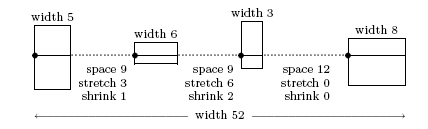
\includegraphics[width=0.9\linewidth]{./images/glue.png}
  \caption{Glue in \TeX}
  \label{fig:glue}
\end{figure}


\section{How to specify glue}

The usual way to specify \textit{glue} to \tex is
$<dimen>< plus~dimen><minus~dimen>$

where the plus and minus are optional and assumed to be zero if not
present; plus\index{glue!plus} introduces the amount of stretchability\index{glue!stretchability}, minus introduces the amount of shrinkability \index{glue!shrinkability}. 

For example, Appendix B of the TexBook defines \cs{medskip} to be an abbreviation for
|\vskip6pt plus2pt minus2p|. The normal-space component of glue must always be
given as an explicit dimen, even when it is zero. The ability of \TeX to stretch and shrink this glue has given it its beautiful looks. Strangely enough, although the algorithm is public it has not been used widely in other software.



\subsection{hfil and hfill}

{\obeylines
{This text will be flush left.\hfil}
{\hfil This text will be flush right.}
{\hfil This text will be centered.\hfil}
{Some text flush left\hfil and some flush right.}
{Alpha\hfil centered between Alpha and Omega\hfil Omega}
{Five\hfil words\hfil equally\hfil spaced\hfil out.}
}

Consider the following definitions:

\begin{verbatim}
\def\centerlinea#1{\hfil#1\hfill}
\def\centerlineb#1{\hfill#1\hfill}
\def\centerlinec#1{\hss#1\hss}
We define quickly a \cs{lineX}\footnote{Strange but my \LaTeX\ distribution has not got on. (This definition is from \texttt{plain.sty}}

\def\lineX{\hbox to\hsize}
\def\lineX{\hbox to\hsize}
\def\centerlinea#1{\hfil#1\hfil}
\def\centerlineb#1{\hfill#1\hfill}
\def\centerlinec#1{\hss#1\hss}

\lineX{\centerlinea{\test}}
\lineX{\centerlineb{\test}}
\lineX{\centerlinec{\test}}
\centerline{\test}
\begin{center}\test\end{center}

\end{verbatim}


\section{Specifying glue amounts}

\tex glue is specified as a fixed dimension, and optionally, with a plus and
or minus dimension. Along with \cs{dimen} registers, TEX has glue registers,
called \cs{skip0} through \cs{skip255}. Here is how you can save glue settings in
\tex registers, and ask \tex to display the contents of one of them:

\begin{teX}
\skip1 = 10pt
\skip2 = 10pt plus 3pt
\skip3 = 10pt minus 2pt
\skip4 = 10dd plus 3dd minus 2dd
\the \skip4
\end{teX}


\texttt{> 10.70007pt plus 3.21002pt minus 2.14001pt}

The four sample glue settings store, respectively, {\em fixed glue}, {\em  stretchable
glue}, {\em shrinkable glue}, and {\em flexible glue}  that can both stretch and shrink,
but only up to a specified amount. Interword and intersentence spaces are
generally defined with glue like this, so that if more stretch or shrink of  a
re underfull (too little text to fill the line), or overfull (too much text in the
line).



\section{Overfull lines}

Although overfull lines are reported in the \tex log file, they can be hard
to find in the typeset document if they only stick out a little. To make
them highly visible while you are fine tuning your final document, assign
the variable \cs{overfullrule} a nonzero dimension, such as 2 cm. \tex then
displays a solid black box, called a \emph{rule}, of that width in the right margin
on each line that is overfull. Using the \docpkg{microtype} package one can adjust the parameters to minimize this.

To make the rules disappear, simply remove it,
or comment out, the assignment, or reset its value to 0 pt. 

Just as you can assign dimension registers to count registers to convert
from points to scaled points, you can assign skip registers to dimension and
count registers to discard the flexible parts:


\begin{teX}
\skip1 = 10pt plus 3pt minus 2pt
\the\skip1
 \dimen1 = \skip1
\the \dimen1
\count1 = \skip1
\the \count1
\end{teX}




\section{More on glue in boxes}

Besides normal glue with fixed amounts of stretch and shrink, \tex also has
two kinds of glue that are \emph{infinitely} stretchable and shrinkable: \cs{hfil} and
\cs{hfill} in horizontal mode, and \cs{vfil} and \cs{vfill} in vertical mode. Notice that there two versions
of the commands, the one ends with one ell and the second one with two. The
two-ell forms are more flexible than the one-ell forms.

The boxes and glue model is powerful, and \tex's author, Donald Knuth,
has written that he views it as the key idea that he discovered when he
first sat down in 1977--1978 to design a computer program for typesetting.
For example, to set something flush left, put infinitely-stretchable glue on
its right. To set it flush right, put the glue on the left. For centered material,
put the glue on both sides. Here are four examples, with vertical
bars marking the ends of the horizontal box (boxes have no visible frames,
although it is possible to write \tex commands to give them such outlines,
and we use that feature shortly):





\section{Horizontal and vertical boxes}


\begin{docCommand}{hbox}{\marg{material}}
\end{docCommand}

Like their dimensions \TeX's boxes are not what one thinks when thinking of boxes. TeX's boxes come in basically two flavours, horizontal boxes and vertical boxes. An \cs{hbox} is created by the command \refCom{hbox}\marg{material}. It has the following properties:

\begin{enumerate}
\item The material is placed from left to right and it becomes a \textit{horizontal list}.\index{horizontal list}
\item The box \textbf{cannot be broken across lines}; it is an indivisible unit.
\end{enumerate}

An |hbox| can contain, characters, horizontal glue, horizontal leaders or other boxes. While in many cases these other boxes can be other |\hbox|es, |\vbox| can be used.


The \refCom{hbox} command has another form |\hbox to <dimen>|\marg{material}. This
creates a box whose width is the given (dimen). Thus |\hbox to lcm{<material>}|
will create a 1 inch wide box \hbox to 1cm{text}. However, we have to supply exactly 1 cm worth of
material to fill up the box; otherwise we end up with an error message. It is best
to consider this form of the command as a promise; we promise '\tex that we will
supply just enough material to fill up the box. 

We can place other hboxes in an hbox. By adding glue we can then move them left or right

\begin{texexample}{hbox and glue}{ex:hbox}
\bgroup
\Huge
\hbox to \textwidth{\hfill \hbox{\EOofficerI}\hbox{\EOofficerII}\hbox{\EOofficerIII} \hfill}

\hbox to \textwidth{\hfill \hbox{\EOofficerI}\hbox{\EOofficerII}\hbox{\EOofficerIII} \hfil}

\hbox to \textwidth{\hfill \hbox{\EOofficerI}\hfill \hbox{\EOofficerII}\hfill \hbox{\EOofficerIII} \hfill}
\egroup
\end{texexample}

The last command that affects the shape of an |\hbox| is 'spread(dimen)', which
spreads the box beyond its natural width. An |\hbox spread12pt|{(material)}
makes the box 12 points wider than its natural size. If the material in the box has
no flexibility, it cannot spread to fill up the additional space, resulting in an underfull
box. This is why 'spread' is normally used with flexible glues.

\begin{texexample}{hbox and glue}{ex:hbox}
\bgroup
\LARGE
\hbox to 5cm{\EOofficerI\EOofficerII\hfill\EOofficerIII}

\hbox spread5cm{\hfill\EOofficerI\hfill\EOofficerII\hfil\EOofficerIII}

\hbox spread9cm{\EOofficerI\hfill\EOofficerII\hfil\hfil\EOofficerIII}

\hbox spread7cm{\EOofficerI\hfill\EOofficerII\hfil\hfil\EOofficerIII} 


\makeatletter
\hb@xt@ 5cm {\EOofficerI\EOofficerII\hfill\EOofficerIII}
\makeatother
\egroup
\end{texexample}



Boxes can be moved up or down using |\raise| or |\lower|. Each of these primitives is followed by a dimension indicating how far the box can be lowered or raised.

Other material that can go in an hbox, is \textbf{vertical rules}. 

\subsection{The null macro}

The |\null| macro is defined both in Plain as well as LaTeX and generates an empty box. Its definition is:

\begin{teXXX}
\def\null{\hbox{}}
\end{teXXX}


\fbox{\hbox{This is a test}}

{
\fbox{\hsize=5cm
A test of a box at the end of a 2.0 inch line\par}

\fbox{\hsize=5.0cm in A test of a box at the end of a \hbox to 2cm{2.0 cm} line\par}

}

What happens when we have more than two boxes on a line? TeX will stuck them one under another. If they are enclosed within another hbox they will be inlined.



\begin{texexample}{}{}
\hbox to 1cm {A} \hbox to 1cm {B}

If we however, put them together in another |\hbox|, we get:

\hbox{\hbox to 1cm {A} \hbox to 1cm{B}}
\end{texexample}




An |\hbox| does not imply horizontal mode, so an attempt to start a paragraph with a box, for
instance
|\hbox to 0cm{\hss$\bullet$\hskip1em}Text ...|

will make the text following the box wind up one line below the box. It is necessary to switch
to horizontal mode explicitly, using for instance |\noindent| or |\leavevmode|. The latter is defined
using |\unhbox|, which is a horizontal command.


\begin{texexample}{}{}
\hbox to 0cm{\hss$\bullet$\hskip1em} Text ...


\leavevmode\hbox to 0cm{\hss$\bullet$\hskip1em} Text ...

\end{texexample}




\section{Kerning}


Using the command \cs{kern}, we can move boxes either left or right. Kerning is extensively used to build internal commands and we discuss it in more detail under the chapter for fonts.

\begin{docCommand}{kern}{\meta{dimen}}
A |\kern| is similar to glue [75], with two differences: (1) |\kern| is rigid; (2)
|\kern| specifies a point where a line, or a page, should not be broken. Since a box is
indivisible anyway, |\kern| is used in a box to indicate rigid spacing. It is interesting
to note that the same command, |\kern|, indicates horizontal spacing when used in
an |\hbox| and indicates vertical spacing when used in a |\vbox|.
\end{docCommand}
Consider two horizontal boxes, holding the letters A and V:
As you can observe, the letters AB are a bit afar, from what would be a visually pleasant arrangement, we can kern them as follows:
\medskip

\begin{teXXX}
\hbox{\Huge AV A\kern-5ptV}
\end{teXXX}
\medskip

Note that hbox, does not produce a frame. I~have used a frame |\fbox|, which will cover a bit later as well as scaled the image by 2, in order to see the effects more clearly.


\drawfontbox{\upshape\Huge FJord F\kern-5pt Jorp}





\noindent\begin{tabular}{ll}
|\hbox{\kern4pt A\kern8pt B\kern8pt C\kern4pt}| & \fbox{\hbox{\kern4pt A\kern8pt B\kern8pt C\kern4pt}} \\
~ &\\
\midrule
|\hbox{\kern4pt\raise1pt\hbox{A}|  & \fbox{\hbox{\kern4pt\raise1pt\hbox{A} \kern8pt BC\kern8pt\lower6pt\hbox{D} \kern4pt} \kern8pt BC\kern8pt\lower6pt\hbox{D}\kern4pt} \\
|\kern8pt BC|                      &\\
|\kern8pt\lower6pt\hbox{D}|        &\\
|\kern4pt}|                        &\\ 
|\kern8pt BC|                      &\\ 
|\kern8pt\lower6pt\hbox{D}|        &\\
|\kern4pt}| &\\
\midrule
\end{tabular}


\vbox{
\noindent\rule{\linewidth}{0.4pt}
\begin{minipage}{4.5cm}
 \begin{teXX}
\fbox{\hbox{\kern4pt A\kern8pt 
      B\kern8pt C\kern4pt}}
\end{teXX}
\end{minipage}
\hfill\hfill
\begin{minipage}{3cm}
\hfill\hfill\fbox{\hbox{\kern4pt A\kern8pt 
      B\kern8pt C\kern4pt}}
\end{minipage}

\medskip
\noindent\rule{\linewidth}{0.4pt}
}

Notice that an |\hbox| is constructed by setting its components side by side so that their \textit{baselines} are aligned. When \cs{raise}, \cs{lower} are used the baselines are no longer aligned. In such a case the baseline of the box is defined as the baseline shared by the components before any vertical movements. In the example above the box now has a depth, as a result of lowering |D|.


\vbox{
\noindent\rule{\linewidth}{0.4pt}
\begin{minipage}{4.5cm}
\begin{teXXX}
\hbox{\kern4pt\raise1pt\hbox{A} 
  \kern8pt BC\kern8pt
  \lower6pt\hbox{D} 
  \kern4pt} 
\end{teXXX}
\end{minipage}
\hfill
\begin{minipage}{3cm}
\fbox{\hbox{\kern4pt\raise1pt\hbox{A} 
\kern8pt BC\kern8pt\lower6pt\hbox{D} \kern4pt}}
\end{minipage}

\medskip
\noindent\rule{\linewidth}{0.4pt}
}



\noindent\textbf{Vertical boxes.}\quad A vertical box is build in a similar manner to that of a horizontal list, except it is composed of material in the \textit{vertical list}.
When horizontal boxes are added in the list, they are stuck on top of each other as shown in the example below. 
\medskip

\bgroup
\parindent0pt
\fbox{\vbox{\hsize=3cm\fbox{\hbox{ABCDEFGH}} \fbox{\hbox{AB}}}}
\egroup


\begin{docCommand}{vbox}{ to \meta{dimen}\marg{\meta{material}}}
Typesets a box in vertical mode.
\end{docCommand}

It is important to remember the two main differences between hboxes and vboxes. An hbox will expand to hold its material. If it need be it will overfill the line and produce an overful warning. A vbox will expand to hold its material. It is perfectly normal for a vbox to hold paragraphs, as shown. This is not possible with an hbox. However, the common pattern is for an |\hbox| to contain a |vbox| .

\begin{texexample}{hbox/vbox example}{ex:vbox}
\noindent\fbox{\vbox{\lorem\par\lorem\par}}

\hbox to \linewidth{\vbox{\lorem\par\lorem\par}}
\end{texexample}


\begin{docCommand}{hsize}{\meta{dimen}}
 Controls the width of text in a |vbox|.
\end{docCommand}

\noindent\textbf{Controlling the size of a vbox.}\quad What controls the size, is the containing environment. This in TeX, is specified using |\hsize|. In LaTeX this is controlled by an enclosing environment, maybe a minipage (which is build this way) or one of the page width parameters.


\begingroup
\parindent0pt
\fboxsep5pt
\hsize=3.9cm\footnotesize
\hfil\fbox{\vbox{\RaggedRight\lorem\par}} 
\hfil\fbox{\vbox{\RaggedRight\lorem\par}}
\hfil\fbox{\vbox{\RaggedRight\lorem\par}}\hfill
\endgroup
\captionof{figure}{Output to demonstrate the use of vboxes.}



The code to typest the boxes shown above follows:
\medskip
\emphasis{hsize}
\begin{teXXX}
\bgroup
\parindent0pt
\hsize=3.3cm\footnotesize
\hfil\fbox{\vbox{\lorem\par}} 
\hfil\fbox{\vbox{\lorem\par}}
\hfil\fbox{\vbox{\lorem\par}}
\hfill
\egroup
\end{teXXX}


Note, the use of \docAuxCommand{hsize}. We define the font size as |\footnotesize|. We have done this in order not to have overfull boxes--Latin words don't have a full set of hyphenation patterns in \latex. The macro |\lorem|, we have defined internally for this document. We place the code in a group in order not to affect the rest of the document.



\clearpage

\noindent\textbf{Vertical centering}\quad can be achieved by applying vertical infinite glue \cs{vfill}. In the example that follows, first we place two letters in individual |\hboxes| and we enclose them in a vbox. We apply |\vfill| both on top and at bottom.

\emphasis{\vfill}

\vbox{
\noindent\rule{\linewidth}{0.4pt}
\begin{minipage}{5cm}
\begin{teX}
\fbox{\vbox to 0.9cm{\vfil\hbox{M}\nointerlineskip\hbox{i}\vfil}} 
\end{teX}
\end{minipage}
\hfill
\begin{minipage}{3cm}
\hfill\fbox{\vbox to 0.9cm{\vfil\hbox{M}\nointerlineskip\hbox{i}\vfil}}\hfill\hfill 
\end{minipage}

\medskip
\noindent\rule{\linewidth}{0.4pt}
}



A |\vbox| can be combined with text and may appear anywhere within a paragraph. The baseline of the box will be aligned with the baseline of the current line.


\vbox{%
\noindent\rule{\linewidth}{0.4pt}}

\begin{teX}
A vbox can be placed within a paragraph \fbox{\vbox to 0.6cm{\vfil\hbox{M}\nointerlineskip\hbox{i}\vfil}} as shown here.


\hfill

A vbox can be placed within a paragraph \fbox{\vbox to 0.6cm{\vfil\hbox{M}
  \nointerlineskip\hbox{i}\vfil}} as shown here.

\end{teX}

\medskip
\noindent\rule{\linewidth}{0.4pt}






\noindent\textbf{Top alignment.}\quad\cs{vtop} is similar to a |\vbox|. The depth of this box is zero, since both A and B are capital letters. The width of this box is |\hsize|, since it contains text. 


\begin{codeexample}[]
\vtop{\hbox{A} \hbox{B}}
\end{codeexample}






Centering a picture in a box, both vertically and horizontally can be achieved using the methods we described so far.


\emphasis{hfill,hbox}
\begin{texexample}{}{}
     \fbox{%
          \vtop{\medskip
                    \hfill
                      \hbox{\includegraphics[width=1.5cm]{./images/amato.jpg}}%
                    \hfill 
                   \medskip%
                }%
      }%
\end{texexample}

\begin{texexample}{}{}
    \fbox{%
          \vtop{\medskip
                    \hfill
                      \hbox{\includegraphics[width=1.5cm]{./images/amato.jpg}}%
                      \hbox{\includegraphics[width=1.5cm]{./images/amato.jpg}}%
                      \hbox{\includegraphics[width=1.5cm]{./images/amato.jpg}}%    
                    \hfill 
                   \medskip%
                }%
      }%
\end{texexample}

Study the example a bit more carefully, as we have said earlier on that \cs{hbox}'es are stacked vertically, the reason why in the above example they are next to each other is that they are in an
\cs{fbox} which in turn is an \cs{hbox}  that can draw  frame around the box and is defined in the
\latex2e kernel.

So if we had only three images in hboxes we will get:

\begin{texexample}{Three Images Lined}{}
%\leavevmode
%\parindent30pt
\hbox{\includegraphics[width=1.5cm]{./images/amato.jpg}}%
\hbox{\includegraphics[width=1.5cm]{./images/amato.jpg}}%
\hbox{\includegraphics[width=1.5cm]{./images/amato.jpg}}%
\end{texexample}

An hbox does not start a paragraph. If we started a paragraph the behaviour will be different.

\begin{texexample}{Three Images Lined}{}
.\hbox{\includegraphics[width=1.5cm]{./images/amato.jpg}}%
\hbox{\includegraphics[width=1.5cm]{./images/amato.jpg}}%
\hbox{\includegraphics[width=1.5cm]{./images/amato.jpg}}%
\end{texexample}

If you notice carefully, we have started the paragraph by inserting a `.' before the first |\hbox|, an alternative way is to 
use |\leavevmode|. The effect of this command is to leave vertical mode, and to enter horizontal mode. Thus, if the mode is vmode (typically, outside any paragraph), a new paragraph is started. This paragraph may be flushed left, flushed right. 

\begin{texexample}{Three Images Lined}{}
\leavevmode
\hbox{\includegraphics[width=1.5cm]{./images/amato.jpg}}%
\hbox{\includegraphics[width=1.5cm]{./images/amato.jpg}}%
\hbox{\includegraphics[width=1.5cm]{./images/amato.jpg}}%

\meaning\leavevmode
\end{texexample}

The macro |\leavevmode| as its name implies forces \tex to leave vertical mode and enter horizontal mode. In this case the photos are just treated by \tex similarly to any character and tehy are typeset next to each other. 

\begin{docCommand}{kern}{}
If we wanted to add a bit of space between the horizontal images, we could use \cs{kern}
Kern again. This is from the book TeX for The Impatient page 157. You can use kern in math mode, but you cannot use the \texttt{mu} units. If you want to use \texttt{mu} units use \cs{mkern} instead.
\end{docCommand}

\emphasize{kern}
\begin{texexample}{}{}
\leavevmode
\hbox{\includegraphics[width=1.5cm]{./images/amato.jpg}}\kern10pt
\hbox{\includegraphics[width=1.5cm]{./images/amato.jpg}}\kern10pt
\hbox{\includegraphics[width=1.5cm]{./images/amato.jpg}}%
\end{texexample}

One needs to be careful as to where you issue |\leavevmode|. If it is in the middle of a paragraph it will have no effect.
\emphasize{This,is,some,text}
\begin{texexample}{Example with leavevmode}{}
This is some text
\leavevmode
\hbox{\includegraphics[width=1.5cm]{botticelli-34.jpg}}\kern10pt
\hbox{\includegraphics[width=1.5cm]{botticelli-34.jpg}}\kern10pt
\hbox{\includegraphics[width=1.5cm]{images/botticelli-34.jpg}}%
\end{texexample}

A very common way in \latex2e is to issue a |\par| command before |\leavevmode| to avoid this problem. Another way is to use
one of the |\ifvmode| or |\ifhmode| and act accordingly. We now fix our example and get what we want. 

\emphasize{par}
\begin{texexample}{}{}
This is some text
\par\leavevmode
\hbox{\includegraphics[width=1.5cm]{botticelli-34.jpg}}\kern10pt
\hbox{\includegraphics[width=1.5cm]{botticelli-34.jpg}}\kern10pt
\hbox{\includegraphics[width=1.5cm]{images/botticelli-34.jpg}}%
\end{texexample}

\begin{texexample}{}{}
   \HHUGE
   \fboxsep=0pt
   \fbox{%
          \vtop{\medskip
                    \hfill
                       \hbox{ H\kern10pt i\kern10pt j}%    
                       \hbox{ A\kern10pt C\kern10pt j}%
                    \hfill 
                   \medskip%
                }%
   }%
\end{texexample}

This example shows how letters are typeset and you can see that they are aligned at the baseline. They are no different than the eimage example that we have shown earlier, except we don't need the boxes.

\medskip

\vbox{
\noindent\rule{\linewidth}{0.4pt}
\begin{minipage}{4.9cm}
\begin{teX}
\centerline{$\Downarrow$}\kern 3pt%
\centerline{$\Longrightarrow$\kern 6pt% horizontal kern
  \textit{A note about kern}\kern 6pt
    $\Longleftarrow$}
\kern 3pt
\centerline{$\Uparrow$}  
\end{teX}
\end{minipage}
\hspace{0.3cm}
\begin{minipage}{4.5cm}
\centerline{$\Downarrow$}\kern 3pt%
\centerline{$\Longrightarrow$\kern 6pt% horizontal kern
  \textit{A note about kern}\kern 6pt
    $\Longleftarrow$}
\kern 3pt
\centerline{$\Uparrow$}
\end{minipage}

\medskip
\noindent\rule{\linewidth}{0.4pt}
}
\medskip

To make a point again, |\vbox| lines boxes at their bottom while, |\vtop| lines them at their top.

\medskip

\vbox{
\noindent\rule{\linewidth}{0.4pt}
\begin{minipage}{4.9cm}
\begin{teX}
 \hbox{\hsize=2cm \raggedright
\vbox to 0.5in{\hrule This box is .5in deep. \vfil\hrule}
\qquad
\vbox to 0.75in{\hrule This box is .75in deep. \vfil\hrule}
\qquad
\end{teX}
\end{minipage}
\hspace{0.3cm}
\begin{minipage}{4.5cm}
\hbox{\hsize=2cm \raggedright
\vbox to 0.5in{\hrule This box is .5in deep. \vfil\hrule}
\qquad
\vbox to 0.75in{\hrule This box is .75in deep. \vfil\hrule}
\qquad}
\end{minipage}

\medskip
\noindent\rule{\linewidth}{0.4pt}
}

\medskip


Trying the same with vtop

\medskip

\vbox{
\noindent\rule{\linewidth}{0.4pt}
\begin{minipage}{4.9cm}
\begin{teX}
 \hbox{\hsize=2cm \raggedright
\vbox to 0.5in{\hrule This box is .5in deep. \vfil\hrule}
\qquad
\vbox to 0.75in{\hrule This box is .75in deep. \vfil\hrule}
\qquad
\end{teX}
\end{minipage}
\hspace{0.3cm}
\begin{minipage}{4.5cm}
\hbox{\hsize=2cm \raggedright
\vtop to 0.5in{\hrule \smallskip This box is .5in deep. \vfil\hrule}
\qquad
\vtop to 0.75in{\hrule \smallskip This box is .75in deep. \vfil\hrule}
\qquad}

\hbox{\hsize=2cm \raggedright
\vbox to 0.5in{\hrule \smallskip This box is .5in deep. \vfil\hrule}
\qquad
\vbox to 0.75in{\hrule \smallskip This box is .75in deep. \vfil\hrule}
\qquad}
\end{minipage}

\medskip
\noindent\rule{\linewidth}{0.4pt}
}

\medskip

There are some other special macros defined by Plain TeX that we will only touch briefly here. One of them is \cs{underbar}{\index{Plain!\textbackslash underbar}.
The macro puts its argument into an hbox and underlines it.

\medskip

\vbox{
\noindent\rule{\linewidth}{0.4pt}
\begin{minipage}{4.9cm}
\begin{teX}
 \underbar{1,000,788.22}
\end{teX}
\end{minipage}
\hspace{0.4cm}
\begin{minipage}{4.0cm}
\medskip
\hfill\hfill{}\hspace*{1em}a1,000,700.22 \hfill

\smallskip

\hfill\[\underbar 1,000,788.22 \]\hfill
\end{minipage}

\medskip
\noindent\rule{\linewidth}{0.4pt}
}

\medskip


The \cs{everyvbox} command inserts a series of tokens at the beginning of every |\vbox|.


\medskip

\vbox{
\noindent\rule{\linewidth}{0.4pt}
\begin{minipage}{4.9cm}
\begin{teX}
 \everyvbox{$\bullet$}...
\end{teX}
\end{minipage}
\hspace{0.4cm}
\begin{minipage}{4.0cm}
\begingroup% Without this group, there are tons of problems!
   \everyvbox{$\bullet$}
   \global\setbox1=\vbox{This is a paragraph without an initial indent. It is   \the\hsize\ long lines.}
   \global\setbox2=\vtop{\copy1}
\endgroup
 \hbox{\box1} 

 \hbox{\box2}
\end{minipage}

\medskip
\noindent\rule{\linewidth}{0.4pt}
}

\medskip
Knuth in the TexBook Chapter 24, has some short description of the every commands. The `everyhbox` inserts a token list just before as its name implies a horizontal box.

Here is a short example. We define a `oneLineBox`, which is simply an hbox with some text and we add spread to spread the line. Using |\everybox| we add the letter \textbf{a} in each horizontal box. 


\tex considers the box overfull if the excess width of the box is larger than \cs{hfuzz} or \cs{hbadness} is less than 100. If I change  the badness to hbadness, I get 1000.

\medskip

\vbox{
\noindent\rule{\linewidth}{0.4pt}
\begin{minipage}{10.0cm}
\begin{teX}
 \begingroup
     \everyhbox{a}
     \def\oneLineBox#1#2%
     {%
          \hfuzz=0pt
          \overfullrule=0.25pt
          \setbox0=\hbox spread#2{#1}%
          \setbox1=\hbox{\the\badness}% 
          \setbox2=\hbox to 4.5cm{\box0\hfil\box1}%
          \box2
     }
     \oneLineBox{Badness of line }{-1em}
     \oneLineBox{Badness of line }{-0.54em}
     \oneLineBox{Badness of line }{-0.4em}
     \oneLineBox{Badness of line }{0em}
     \oneLineBox{Badness of line }{1em}
     \oneLineBox{Badness of line }{2em}
     \oneLineBox{Badness of line }{3em}
 \endgroup
\end{teX}
\end{minipage}


\begin{minipage}{10.0cm}
\begingroup
     \everyhbox{a}
     \def\oneLineBox#1#2%
     {%
          \hfuzz=0pt
          \overfullrule=0.25pt
          \setbox0=\hbox spread#2{#1}%
          \setbox1=\hbox{\the\badness}% 
          \setbox2=\hbox to 4.5cm{\box0\hfil\box1}%
          \box2
     }
     \oneLineBox{Badness of line }{-1em}
     \oneLineBox{Badness of line }{-0.54em}
     \oneLineBox{Badness of line }{-0.4em}
     \oneLineBox{Badness of line }{0em}
     \oneLineBox{Badness of line }{1em}
     \oneLineBox{Badness of line }{2em}
     \oneLineBox{Badness of line }{3em}
 \endgroup
\end{minipage}

\medskip
\noindent\rule{\linewidth}{0.4pt}
}

\medskip










\parindent1em




\section{More features of horizontal boxes}

Characters in the Latin alphabet have different shapes, and in most typefaces,
different widths. The letters \texttt{d f h k l t} have ascenders, making them
higher than the vowels \texttt{a e o u}, while the letters \texttt{f g j p q y} have descenders,
giving them added depth below the vowels. Similarly, an \texttt{m} is wider than
an \texttt{i}. 

\drawfontbox{(fjord)}

When \tex makes a normal horizontal box, the box width is the sum
of the widths of the characters, and the fixed parts of any glue, contained
in it. Shrink and stretch components of glue are discarded for the width
calculation. The box also has both a height above the baseline, the invisible
line on which the characters rest, and a depth below the baseline. The
depth is zero if there are no objects with descenders. The height and depth
are chosen from the largest vertical extents of the contained objects.

If you look carefully at typeset material, you will observe that, in most
typefaces, parentheses, brackets, and braces have both descenders and ascenders,
and the typeface designer usually makes their extents the maximum
among all of the characters in the design. This sample text shows
document: ( h g ) [ k j ] { l p }.

You can force TEX to choose a larger height and depth than normal when
you write a command for a horizontal box by ensuring that it has suitable
contents, such as an invisible vertical rule of zero width. The command

\verb+\hbox to 50pt {\vrule height 20pt depth 10pt width 0pt \it stuff}+

produces a box whose (invisible) outline looks like this: 

\hbox to 50pt {\vrule height 20pt depth 10pt width 0pt \it Great}

\drawfontbox{\kern 5pt\vrule height20pt depth 10pt width 1pt fjord}

The
three extents of the vertical rule can appear in any order, and any convenient
units.

In order to see the otherwise-invisible box edges in that example, we
used the \latex  built-in command \cs{fbox} to create a frame, and we eliminated
the default margin inside the frame by setting \cs{fboxsep = 0pt}. Plain \tex
does not have the \cs{fbox} command, but The TEXbook shows how to make
something like it on pp. 223 and 321.

One particular zero-width vertical rule is convenient for ensuring that
separate boxes all get the same height and depth. It has the height and
depth of parentheses in the normal prose font, and is given the macro name \refCom{strut}.
Its definition in the plain.tex file of macro definitions is roughly
equivalent to this:

\begin{docCommand}{strut}{}
\end{docCommand}

\begin{teX}
  \def \strut {\vrule height 8.5pt depth 3.5pt width 0pt}
\end{teX}

We insert a |\vrule| at the figure on the left below with a height of 20pt and a depth of 10pt. You can observe the difference on the right box, without the |\vrule|. The \textit{strut} is the blue line, which we gave a width of one point to make it visible. Real life struts, would have a width of 0pt and will not be visible. 

\drawfontbox{\kern5pt{\color{blue}\vrule height20pt depth 10pt width 1pt} fjord}
\drawfontbox{fjord}



\section{Horizontal alignment of boxes in TEX}
\fboxsep0.4pt

When horizontal boxes are set together, they are treated as separate words,
and therefore spaced accordingly. The input
\verb+ \fbox{one} \fbox{two} \fbox{three} \fbox{four}  +
produces  \fbox{one} \fbox{two} \fbox{three} \fbox{four}. As the example shows, we can put spaces
between them, or run them together so that they fit tightly.


\section{Vertical boxes in TEX}


\begin{minipage}{2.0in}
\begin{verbatim}
\noindent
\fbox{%
  \it
  \hbox to 80pt{%
     \parindent = 0pt
     \vbox to 30pt {%
         left text
         \vfil
         more left text%
     }%
  }%
}%
\end{verbatim}
\end{minipage}


%\noindent
\fbox{%
  \it
  \hbox to 80pt{%
     \parindent = 0pt
     \vbox to 30pt {%
         left text
         \vfil
         more left text%
     }%
  }%
}%

Firstly we use a noindent to ensure that the box is not indented. If you comment the\cs{fbox} out, you can see that the right amount of space has been left in the paragraph above.

\mbox{}
 
\noindent
\fbox{%
\it
\hbox to 80pt{%
\parindent = 0pt
\hsize = 80pt
\vbox to 30pt {\hfill right text
\vfil
\hfill more right text}
}%
}%



\noindent
\fbox{%
\it
\hbox to 80pt{%
\parindent = 0pt
\hsize = 80pt
\vbox to 30pt {\hfil center text
\vfil
 more center text \hfil}
}%
}%

We can aslo center the text for both lines, by modifying the code slightly.
\begin{teX}
\noindent
\fbox{%
\it \hbox to 80pt{
   \parindent = 0pt
   \hsize = 80pt
   \vbox to 30pt {
   center text \hfill
    \vfil
    \hfil more center text}
   }%
}%
\end{teX}


\noindent
\fbox{%
\it
\hbox to 80pt{%
\parindent = 0pt
\hsize = 80pt
\vbox to 30pt {\hfil center text
\vfil
\hfil more center text}
}%
}%



\chapter{Boxes with \protect\LaTeXe}

The \tex primitive commands have been abstracted by \latexe into more user friendly commands that are easier to use. One other reason for using these \LaTeX\ commands is that they are ``color safe''. Later on we will see other possibilities given by the \pkgname{color} or \pkgname{xcolor} package for drawing colored boxes, but we want to recall that the code for |\makebox| and the like has already a protection mechanism for colors, which the primitive commands do not have. \latexe also provides boxes that are self-aware of the width of their contents. For example |\fbox| will frame its contents in an |\hbox|. This simple task is very convoluted to achieve using basic \tex commands. 

\begin{docCommand}{framebox} {\marg{dim}}
One useful box command provided by \latex2e is \cmd{\framebox}. This command builds a box with any material you want to provide it with. The contents of this box are unbreakable, and as far as \tex is concerned it is treated the same way as it would treat a letter. 
\end{docCommand}

\begin{docCommand}{fboxsep}{\marg{dim}}
\end{docCommand}
\begin{docCommand}{fboxrule}{\marg{dim}}
Two associated lengths control the width of the rule and the space around the contents. We can change their default value by using |\setlength{\fboxsep}{0pt}| or just simply |\fboxsep=0pt| or even |\fboxsep0pt|. 
\end{docCommand}


Another interesting property is this: \emph{the contents of a box need not lie inside it}. You may have
noticed that, given the contents as an argument, the
|\framebox| command sets the dimensions of the box
to those of the contents (in reality, to the ``sub-boxes"
that compose the contents). But you can define the
dimensions explicitly as well. For example,

\begin{texexample}{framebox example}{ex:framebox}
|\framebox[13em]{Some text}|

\framebox[13em]{Some text}

\fcolorbox{theblue}{cyan}{Some text}

\end{texexample}

The box as is shown in the example will not break and it occupies more space than its contents. A second optional command allows us to typeset the contents, left, center or right.

\begin{codeexample}[vbox]
\fboxrule1pt

\framebox[13em][l]{Some text}\par

\framebox[13em][r]{Some text}\par

\framebox[13em][c]{Some text}\par

\framebox[1em][l]{Some text}\par

\framebox[1em][c]{Some text}\par

\framebox[1em][r]{Some text}\par
\end{codeexample}

As you can observe \latexe has abstracted the |\hfill| and similar commands and allows boxes to be constructed with ease. We have started the discussion with |\framebox|, but most practical uses of boxes is when they remain invisible.

\begin{docCommand}{makebox} { \oarg{width}\oarg{position}\marg{contents} } 
 is \latex's box workhorse.
 \end{docCommand}

The |source2e| manual states. If the width is missing, then position is also missing and |obj|  is put in an \cs{hbox} of its natural width. This is true as far as the looks are concerned, but not the behaviour, as you can see
from the following example is not an unqualified \cmd{\hbox} it is an hbox preceded by leavevmode.\footnote{\url{http://tex.stackexchange.com/questions/105585/latex2e-makebox-hbox}} This is of course good practice and brings consistency to the LaTeX kernel. I would recommend that you follow such practices in your own code. 

\begin{texexample}{}{}
\newbox\temp
\savebox\temp{test}
LaTeX

\makebox{test} \mbox{test}

TeX

\hbox{test} \hbox{test}

\indent\hbox{test} \hbox{test}

LaTeX with \cs{leavemode}

\makeatletter
\leavevmode\hbox to \wd\temp{test} \indent\hbox to \wd\temp{test}
\makeatother
\end{texexample}



\latex's analog of a\cs{hbox} is called \cs{mbox}. They are 
much the same thing, but \cs{mbox} is defined to be more widely usable. We have already used \latex's framed companion to \cs{mbox}, \cs{fbox}.

A horizontal box of specified width is provided in \latex with the command
\doccmd{makebox[width][position]\{contents\}}. Bracketed command arguments
in \latex are always optional. 

Here, the width is a \tex dimension,
and defaults to the natural width of the contents if not given. The position
is one of the letters \textbf{l} (flush left) or \textbf{r} (flush right); if it is omitted, the text
is centered in the box. If the specified width is smaller than needed, the
contents protrude from the box, and may overlap surrounding material. If
the specified width is zero, then we have equivalents of the TEX \cs{rlap} and
\cs{llap} commands.


Here are several examples of these three LATEX box commands:

{\obeylines
\mbox{stuff}

\fbox{stuff} 

|\makebox{stuff}|

|\makebox[40pt][l]{stuff}|

|\makebox[40pt][r]{stuff}|

|\makebox[0pt]{stuff}|

|\makebox[0pt][l]{stuff}|

|\makebox[0pt][r]{stuff}|
}



\subsection{Positioning boxes}

To help in positioning boxes within other objects, \latex provides the command
\docAuxCmd{raisebox} to raise and lower boxes:

\begin{teX}
\raisebox{raiselength}[height][depth]{contents}
\end{teX}

A negative first argument lowers the box, where the \cmd{\lowerbox} will lower the box. Here are some examples:

\begin{texexample}{Raising and lowering boxes}{ex:raise}
A \raisebox{10pt}{\fbox{upper}} A
upper
A \raisebox{10pt}{\
fbox{lower}} A
lower
A \fbox{\raisebox{10pt}[25pt]{\fbox{upper}}} A
upper
A \fbox{\raisebox{10pt}[
25pt]{\fbox{lower}}} A
lower
A \fbox{\raisebox{10pt}[25pt][15pt]{\fbox{upper}}} A
upper
A \fbox{\raisebox{10pt}[
25pt][15pt]{\fbox{lower}}} A
lower
\end{texexample}

\section{Paragraph Boxes}

\begin{docCommand}{parbox}{\oarg{position}\oarg{height}\oarg{innerpos}\marg{width}\marg{contents} }
  For longer strings of text, \latex provides the paragraph box \cs{parbox} 
\end{docCommand}


The optional position
is a letter \textbf{b} for alignment of the bottomline with the current baseline,
or \textbf{t} for alignment of the top line with the surrounding baseline. Without

The box can be used as if it were a letter or a word, so we can put it in
the middle of a sentence. The input

This is text \parbox{30pt}{\it and this is boxed text} and
this is more text.

This is text \fbox{\parbox{30pt}{\it and this is boxed text}}
and this is more text.
produces


Flush-right typesetting generally looks bad in narrow columns, so we
can insert a \cs{raggedright} command inside the last argument of the paragraph
box to get output like this:

\begin{texexample}{}{}

\parbox[b][120pt][t]{130pt}{\lorem}%
\hspace{1cm}%
\parbox[b][150pt][t]{130pt}{Only some short line of text here.}%



\parbox[b][120pt][t]{130pt}{\lorem}\hspace{1cm}\parbox[b][120pt][c]{130pt}{Only some short line of text here.}

\end{texexample}


\section{The minipage environment}

Another kind of paragraph box can be obtained in a more general, and
more powerful, way with the \docAuxEnv{minipage} environment:

\emphasis{minipage}
\begin{phdverbatim}
\begin{minipage}[position]{width}
   contents
\end{minipage}   
\end{phdverbatim}


The positioning works just like that for \verb+\parbox+, with alignment letters \textbf{b}
and \textbf{t}, and if they are omitted, a default of vertical centering.
In particular, verbatim text produced with the verb command is illegal
in macro arguments, so it cannot be used with \cs{fbox}, \cs{framebox}, \cs{makebox},
\cs{mbox}, or\cs{ parbox}, but it can be used inside a minipage. The input


\begin{texexample}{}{}
\begin{minipage}{170pt}
This is inline verbatim \verb=\verb|\%{}|=, and this
is a verbatim display:

\begin{verbatim}
#include <stdio.h>
#include <stdlib.h>
int main(void)
{
  printf("Hello, world\n");
  exit (EXIT_SUCCESS);
}
\end{verbatim}
\end{minipage}

\end{texexample}


A minipage can go everywhere and can hold virtually any content.


\section{Scaling and resizing boxes}

\begin{docCommand}{resizebox}{\marg{width}}{\marg{general material}}
Resizes the contents of a box
\end{docCommand}

The command \cs{resizebox}\marg{width}\marg{height}\marg{object} can be used with tabular to specify the height and width of a table. The following example shows how to resize a table to 8cm width while maintaining the original width/height ratio.

\begin{teX}
\resizebox{8cm}{!} {
  \begin{tabular}...
  \end{tabular}
}
\end{teX}

Alternatively you can use \cs{scalebox}{ratio}{object} in the same way but with ratios rather than fixed sizes:

\begin{teX}
\scalebox{0.7}{
  \begin{tabular}...
  \end{tabular}
}
\end{teX}

Both |\resizebox| and |\scalebox| require the \pkg{graphicx}\footfullcite{graphicx} package.
To tweak the space between columns (LaTeX will by default chose very tight columns), one can alter the column separation: |\setlength{\tabcolsep}{5pt}|. The default value is |6pt|.

The scalebox is great if you want to magnify a letter so that you can observe the design closer.

\bigskip
\noindent\begin{tabular}{|c|c|c|c|c|c|}\hline
Kp-Fonts & Kp-\textit{light} & CM & Palatino & Utopia & Times\\\hline\hline
\scalebox{2}{ag713} &
\scalebox{2}{\fontfamily{jkpl}\selectfont 7} &
\scalebox{2}{\fontfamily{lmr}\selectfont 713}  &
\scalebox{2}{\fontfamily{ppl}\selectfont 713}  &
\scalebox{2}{\fontfamily{put}\selectfont 7} &
\scalebox{2}{\fontfamily{ptm}\selectfont \oldstylenums{7}} \\\hline
\end{tabular}


\begin{teX}
\hspace{-6mm}\begin{tabular}{|c|c|c|c|c|c|}\hline
Kp-Fonts & Kp-\textit{light} & CM & Palatino & Utopia & Times\\
\hline\hline
  \scalebox{10}{a} &
  \scalebox{10}{\fontfamily{jkpl}\selectfont a} &
  \scalebox{10}{\fontfamily{lmr}\selectfont a}  &
  \scalebox{10}{\fontfamily{ppl}\selectfont 7}  &
  \scalebox{9.2}{\rule{0pt}{1.25ex}\fontfamily{put}\selectfont a} &
  \scalebox{10}{\fontfamily{ptm}\selectfont a}\\\hline
\end{tabular}
\end{teX}
\bigskip



\section{Glues with Negative and zero dimensions}

A box with a natural size of zero with the right glue amount can become very useful. For example the glue
|0pt plus1fil minus1fil| can stretch to infinity and also shring to minus infinity. Of course in the case of
\tex infinity is \docAuxCommand{maxdimen}. A \tex primitive is defined with this glue \refCom{hss}.

\begin{docCommand}{hss}{}
\end{docCommand}

There is also a corresponding \refCom{vss}.

\begin{docCommand}{vss}{}
\end{docCommand}


These macros place text on a full line either centred or left or right adjusted.

\begin{texexample}{}{}
\makeatletter
368 \def\@@line{\hb@xt@\hsize}
369 \def\leftline#1{\@@line{#1\hss}}
370 \def\rightline#1{\@@line{\hss#1}}
371 \def\centerline#1{\@@line{\hss#1\hss}}
\rlap
\llap
These macros place text to the left or right of the current reference point without
taking up space.
372 \def\rlap#1{\hb@xt@\z@{#1\hss}}
373 \def\llap#1{\hb@xt@\z@{\hss#1}}

$a\mathrel{\rlap{\;/}{=}}b $

{\Huge
\leavevmode
\rlap{Y}L
\rlap{C}\kern2.6pt\lower3.5pt\hbox{,}
}
\makeatother
\end{texexample}

\begin{docCommand}{rlap}{\marg{material}}

\end{docCommand}

Of course neither |llap| or |rlap| start a paragraph, so we need to use a |leavevmode| or one of the other ways to start a paragraph.

\begin{docCommand}{llap}{\marg{material}}
\end{docCommand}


\begin{docCommand}{smash}{\marg{material}}
The |\smash| command typesets the material with a height and depth of zero.
\end{docCommand}

\begin{docCommand}{phantom}{\meta{material}}
\end{docCommand}

\begin{docCommand}{vphantom}{\meta{material}}
\end{docCommand}

\begin{texexample}{Defining smash}{}
\bgroup
\def\smash{%
   \relax % \relax, in case this comes first in \halign
   \ifmmode
   \expandafter\mathpalette\expandafter\mathsm@sh
   \else
    \expandafter\makesm@sh
   \fi}
   
\def\makesm@sh#1{%
   \setbox\z@\hbox{\color@begingroup#1\color@endgroup}\finsm@sh}

\def\mathsm@sh#1#2{%
   \setbox\z@\hbox{$\m@th#1{#2}$}\finsm@sh}

\def\finsm@sh{\ht\z@\z@ \dp\z@\z@ \box\z@}
\egroup

\vbox{\smash {\hbox{A} } \hbox{B}} Test

\end{texexample}

\cxset{geometry units = pt,
       fontbox font=\Huge\upshape}

  


Consider the letters `Q' and `P', shown below. The capital letter `Q' has a depth of 1.72mm, we might wish to smash
it in a two line title block to reduce the line spacing between two consecutive lines. This can be accomplished with the
\refCom{smash} command.

\centerline{\drawfontbox{Q} \drawfontbox{P}}

Smashing it produces the following results.

\centerline{\drawfontbox{\vbox{\smash {\hbox{Q} } \hbox{P}}}  \drawfontbox{\vbox{\hbox{Q}  \hbox{P}}}}  

The command is more useful in math environments and is used extensively both by authors and package developers.

\begin{teXXX}
\def\rightarrowfill{$\m@th\smash-\mkern-7mu%
454 \cleaders\hbox{$\mkern-2mu\smash-\mkern-2mu$}\hfill
455 \mkern-7mu\mathord\rightarrow$}

456 \def\leftarrowfill{$\m@th\mathord\leftarrow\mkern-7mu%
457 \cleaders\hbox{$\mkern-2mu\smash-\mkern-2mu$}\hfill
458 \mkern-7mu\smash-$}
\end{teXXX}

Two further macros can be useful to authors of mathematical documents, \docAuxCommand*{phantom} and \docAuxCommand*{vphantom}. 

When typesetting roots, sometimes there are issues with heights. The following example
from \citetitle{mathmode}\footcite{mathmode} illustrates the point.

\begin{equation}
 \sqrt{a}\,%
 \sqrt{T}\,%
 \sqrt{2\alpha k_{B_1}T^i}\label{eq:root1}
\end{equation}

This can be corrected using \refCom{vphantom}. 

\begin{texexample}{Correcting height issues}{ex:sqrtheights}
\begin{equation}\label{eq:root2}
 \sqrt{a\vphantom{k_{B_1}T^i}}\,%
 \sqrt{T\vphantom{k_{B_1}T^i}}\,%
 \sqrt{2\alpha k_{B_1}T^i}
\end{equation}

\begin{equation}
x = \sqrt[3]{6+\sqrt[3]{6+\sqrt[3]{6+\sqrt[3]{6+\cdots}}}}
\end{equation}
\end{texexample}

Using \pkgname{amsmath} \docAuxCommand{smash} can be used for even better results when
using inline or displayed roots. It must be noted that \cs{smash} in \latexe is defined
without such an optional argument.



\makeatletter
\renewcommand{\smash}[1][tb]{%
\def\mb@t{\ht}\def\mb@b{\dp}\def\mb@tb{\ht\z@\z@\dp}%
\edef\finsm@sh{\csname mb@#1\endcsname\z@\z@ \box\z@}%
\ifmmode \@xp\mathpalette\@xp\mathsm@sh
\else \@xp\makesm@sh
\fi
}
\makeatother
This is a test $\sqrt{\lambda_{ki}}$ and $\smash[tb]{\sqrt{\lambda_{ki}}} $ 
\meaning\smash

\begin{docCommand}{smash}{ \oarg{position}\marg{argument} }
The optional argument for the position can take three values: \textbf{t} keeps the bottom and annihilates the top, \textbf{b} keeps the top and annihilates the bottom and \textbf{tb} which annihilates top and bottom. The latter is the default.
\end{docCommand}

\begin{texexample}{Use of Amsmath smash}{ex:amssmash}
xxx
\fbox{\rule{0.5cm}{2cm}}
\fbox{\rule[-1cm]{0.5cm}{2cm}}
\fbox{\smash{\rule{0.5cm}{2cm}}}
\fbox{\smash{\rule[-1cm]{0.5cm}{2cm}}}
\fbox{\raisebox{0pt}[0pt][0pt]{\rule[-1cm]{0.5cm}{2cm}}}
\fbox{\raisebox{-1cm}[0pt][0pt]{\rule{0.5cm}{2cm}}}
\end{texexample}


\begin{texexample}{The array environment}{ex:array2}
Thus to change $\frac34$ to a decimal divide $4$ into $3$
and we get $.75$ as a result, thus:
\[
\begin{array}{r@{}r@{}}
4 \; & \vline \; 3.00 \\\cline{2-2}
     &            .75
\end{array}
\]
To find the square root of a four-figure number
such as our example calls for, work it out in the
following manner:


\[
\arraycolsep=0em
\begin{array}{cccccccccccc}
\multicolumn{3}{c}{\text{2d pair}} &\qquad&\qquad&
\multicolumn{3}{c}{\text{1st pair}}&\qquad&\qquad&
\multicolumn{2}{c}{\text{square root}}\\
 & \overbrace{\quad}&\ZZZ&&&\ZZZ&\overbrace{\quad}&\ZZZ\\
 & 42 &&&&& 25 &&&&\vline\;65&(answer)\\\cline{11-11}
 & 36 &&&&& \\\cline{2-2}
\multirow{2}{*}{125\:} & \vline\hfill \phantom{Z}6 \hfill&&&&& 25\\
 & \vline\hfill \Zi6 \hfill&&&&& 25\\\cline{2-7}
\end{array}
\]
\end{texexample}

What I provided as an easy mnemonic for the \pkg{phd} I provided macros |\Zi, \ZZ, \ZZZ| as convenience aliases for
|\phantom{Z}| etc.

With graphic programs becoming available, most of the drawing of small complicated boxes, has been overtaken by using
\tikzname and especially its option to overlay a node at a particular point of the page without any impact on the spacing.







 %passbiber
  %\cxset{custom = fashion,
%          fashion image=./images/venus.jpg}

\chapter{Rules and Leaders}
\pagestyle{headings}

\epigraph{He had forty-two boxes, all carefully packed,
With his name painted clearly on each:
But, since he omitted to mention the fact,
They were all left behind on the beach.}{---Lewis Carroll, The Hunting of the Snark}

\section{Rules}

Rules, both horizontal and vertical, are traditionally used in typesetting. In
\tex, a rule does not necessarily have to be long and thin; it has three dimensions,
like a box, and can have any rectangular shape. There are two types of rules, |\hrule| and |\vrule|.

\begin{docCommand}{hrule}{ height\meta{dimen} width \meta{dimen} depth\meta{dimen} }
Draws a rule in vertical mode.
\end{docCommand}

\begin{docCommand}{vrule}{ height\meta{dimen} width \meta{dimen} depth\meta{dimen} }
Draws a rule in horizontal mode.
\end{docCommand}

The shape of the rule does not depend on whether it is \textsc{h} or \textsc{v}, and the difference
between the two types is in the context in which they can be used, not in their
shapes. An |\hrule| is considered vertical material and can be part of a vertical list.

A |\vrule| is the opposite and can only appear in horizontal lists. The reason for
this convention is that a horizontal rule is a good separator between items stacked
vertically, whereas a vertical rule is a natural separator for items laid horizontally,
from left to right.

As a result, a |\vrule| should be used inside a paragraph, such as this \vrule, or in
an |\hbox|. An |\hrule| should be used between paragraphs or in a |\vbox|.

Any unspecified dimensions of a rule are determined [221] by these defaults:

\begin{enumerate}
\item The height of an |\hrule| is 0.4pt, and the depth is 0pt.
\item The width of a |\vrule| is 0.4pt.
\item Other dimensions are determined by extending the rule to the size of the smallest
box containing it. An example of this rule is the |\vrule| above. Its depth is set
equal to the depth of the line it happens to be on.
\end{enumerate}



The rule is extended to the width {\Huge \drawfontframe{\vbox{\hsize=24pt\parindent0pt p\hrule*}}}

\paragraph{Struts} The word \emph{strut} has already been mentioned. It refers to a \refCom{vrule} with width zero. It refers to a |\vrule| with
width zero. A standard strut is part of the plain format and is defined, on [353], as
|\vrule height8.5pt depth3. 5pt width0pt| (the actual definition is slightly more
complicated and takes into account the current mode). Such a rule does not show
up in print and is used to open up boxes. Inexperienced users find it hard to believe
that such a rule can be useful, but a glance at [478] shows that it is one of the most
frequently mentioned terms in the \texbook.

A horizontal strut can also be defined. It is an |\hrule| with height and depth
of zero. Surprisingly, such a thing is rarely used (but see discussion of |\hphantom|
in section 3.24)

\begin{texexample}{Drawing a Ruler}{ex:ruler}
\bgroup

\def\1{\vrule height 0pt depth 2pt}

\def\2{\vrule height 0pt depth 4pt}

\def\3{\vrule height 0pt depth 6pt}

\def\4{\vrule height 0pt depth 8pt}

\def\ruler#1#2#3{%
    \leftline{$\vcenter{%
    \hrule\hbox{\4#1}}\,\,\rm#2\,{#3}$}}%
  
\def\\#1{\hbox to .125in{\hfil#1}}
  
\def\8{\\\1\\\2\\\1\\\3\\\1\\\2\\\1\\\4}%
  
\ruler{\8\8\8\8}4{in}
\egroup
\end{texexample}

Lamport in \latex developed a macro |\rule| to enable users to draw lines without remembering all the rules for horizontal or vertical modes and the like.\footnote{In the latest releases this has been changed to a robust macro, using \textbackslash DeclareRobustCommand.}

\begin{docCommand}{rule}{\oarg{raised}\marg{width}\marg{height} }
Typesets a rule with a  \meta{width} and\meta{height}, raised by \meta{raised}.
\end{docCommand}

\begin{teX}
\def\rule{\@ifnextchar[\@rule{\@rule[\z@]}}%
\def\@rule[#1]#2#3{%
\leavevmode
\hbox{%
  \setlength\@tempdima{#1}%
  \setlength\@tempdimb{#2}%
  \setlength\@tempdimc{#3}%
  \advance\@tempdimc\@tempdima
  \vrule\@width\@tempdimb\@height\@tempdimc\@depth-\@tempdima}
}
\end{teX}

The important macro is |@rule| which sets the lengths and widths to the parameters required by the user. The raising of the rule is achieved by adjusting the depth to the given amount of length to raise the rule.

This is a Lamport rule |\rule[6.5pt]{4pt}{7pt}| typeset as:\rule[6.5pt]{4pt}{7pt} Many \latexe packages 
provide rules for common cases, such as \pkg{booktabs} providing rules that can be used in tables. 

Another useful \latexe macro is |\underline| that can be used to underline text. The \latex version is a modification of the \textsc{plain} version to enable it to be used in math mode. The \textsc{plain} version can still be used in \latexe by using |\@@underline|. 

\section{Applications}

One example of \refCom{vrule} is to provide the color background of a box. This method is used for
example by the \pkg{xcolor} to provide generic drivers. First a |vrule| with the require box dimensions
is typeset in a zero width box using \refCom{rlap} and then the text is overwritten to provide the typeset box, with a background color. One can extend such macros to draw numerous lines at different colors to also 
achieve  a gradient effect.


\begin{texexample}{}{}
\makeatletter
\bgroup
\renewcommand*\color@block[3]%
{{%
\color{blue}%
    \rlap{%
      \ifcolors@
        \vrule\@width#1\@height#2\@depth#3
      \fi
    }%
}} 
\hbox{\color@block{80pt}{30pt}{3.5pt}%
      \sffamily\bfseries\Huge\color{white}FFji}
\egroup 
\makeatother 
\end{texexample}

Of course the example is trivial. In a more detailed macro, it would be preferable to measure the dimensions
of the text and size the background accordingly. 

\section{Leaders}

A leader is a single copy of a pattern, for example in a dashed line a dash is a leader.
Dot leaders are a row of dots that visually connect the chapter titles and section headings to their corresponding page numbers. 

Leaders don't have to be composed of dots, with \tex leaders can be used fill a space with copies of a pattern,
\eg, to put repeated dots between a title and a page number in a table
of contents. 

The Plain Format provides six standard leader definitions. All these definitions are equivalent to an |\hfill| type of horizontal glue.

\medskip

\begin{tabular}{lp{3cm}}
\docAuxCommand{hrulefill}     & \hrulefill\\
\docAuxCommand{dotfill}        & x\dotfill x \\
\docAuxCommand{leftarrowfill} & \leftarrowfill\\
\docAuxCommand{rightarrowfill} & \rightarrowfill\\
\docAuxCommand{downbracefill} & \downbracefill\\
\docAuxCommand{upbracefill} & \upbracefill\\
\end{tabular}
\bigskip


A leader is a single copy of the pattern. The specification of
leaders contains three pieces of information:

\begin{enumerate}
\item  what a single leader is
\item  how much space needs to be filled
\item  how the copies of the pattern should be arranged within the space
\end{enumerate}

In \tex leaders are actually \emph{visual glue}. Wherever glue can go a row of leaders can go.

\begin{texexample}{Leaders}{ex:leaders}
\meaning\dotfill  \par
\meaning\hrulefill\par
\meaning\downbracefill\par
\end{texexample}

\begin{docCommand}{leaders}{}
\tex applies an imaginary window and only those leader boxes are printed which fully fit into the window. This ensures that the leader dots of different lines line up vertically.
\end{docCommand}


\begin{docCommand}{cleaders}{}
\end{docCommand}

\begin{docCommand}{xleaders}{}
\tex  provides three commands for specifying leaders:\cs{leaders},\cs{cleaders},
and\cs{xleaders} (p.~174). The argument of each command specifies the
leader. The command must be followed by glue; the size of the glue specifies
how much space is to be filled. The choice of command determines how
the leaders are arranged within the space.
\end{docCommand}

Rule leaders \textit{fill} the specified amount of space with a rule extending in the direction of the skip
specified. \index{rules and leaders>rule leaders}

The most common application for leaders is to fill the space with either a rule or with dots, such as shown in Example~\ref{leaders} below.

\emphasis{leaders,hbox,hfill}
\begin{texexample}{Leader example}{leaders}
\hbox{Exa\leaders\hrule\hskip20pt e}
\hbox to \linewidth{Section 1.2 \leaders\hbox{..}\hfill\space 15}
Section 1.3 \leaders\hbox{..}\hfill\space 15

\parfillskip=0pt plus1fil

\lipsum*[1]\leaders\hbox{..}\hfill\space 15
\end{texexample}

Leaders must be in a box, such as an \cs{hbox}. If they are not in a box an error is issued by \tex.

\begin{texexample}{}{hboxleaders}
\hbox to \textwidth{g\leaders\hbox{+}\hfill 112}
\end{texexample}

because a horizontal rule has a default height of |.4pt|. On the other hand,\index{Rules and Leaders>default value}

\verb+\hbox{g\leaders\vrule\hskip10pt f}+

gives

\hbox{g\leaders\vrule\hskip10pt f}

because the height and depth of a vertical rule by default fill the surrounding box.
Spurious rule dimensions are ignored: in horizontal mode

\verb+\leaders\hrule width 10pt \hskip 20pt+

is equivalent to

\verb+\leaders\hrule \hskip 20pt+

If the width or height-plus-depth of either the skip or the box is negative, TEX uses ordinary glue
instead of leaders.

\section{Box leaders}
\index{leaders box}
Box leaders fill the available spaces with copies of a given box, instead of with a rule. The first example uses \latex3 syntax, which is bound to send old \tex masters into an apoplectic fit. However, once your eyes
and brains absorb the syntax, \latex3 is too good to be ignored and can be mastered in a month or so. The
underscores still bother me, as well as the Hungarian notation, but I have mellowed as I grew older and
have now accepted it as an essential toolbox for latexing.

The reason I introduced it here, is to get you used to it for the next chapter, which is dedicated to \latex3 boxes and skips. This will bring us to a full round. We have studied the original \tex and plain format commands, the \latex2e and next the \latex3 macros. 

\begin{texexample}{Box leaders}{}
\ExplSyntaxOn  
  \box_new:N \starbox
  %\setbox\starbox=\hbox:n{
  \hbox_set:Nn \starbox 
    {
      \skip_horizontal:n { .2em  }
      \box_move_down:nn { 2.5pt }
                        {\hbox:n{*}}
      \skip_horizontal:n {.2em}
    }

  
  \hbox_to_wd:nn {\textwidth} 
    {
       \null \tex_leaders:D\box_use:N \starbox \hfill \null
    }.
\ExplSyntaxOff
\end{texexample}

If you notice you have to use the \cs{copy} command rather than \cs{usebox}, as we cannot use the |\leavevmode| with leaders

\begin{verbatim}
\usebox unchanged
81 \def\usebox#1{\leavevmode\copy #1\relax}
\end{verbatim}

That is, copies of the box register fill up the available space.

Dot leaders, as in the above example, are often used for tables of contents. In such applications it
is desirable that dots on subsequent lines are vertically aligned. The\cs{leaders} command does this
automatically:


The mechanism behind this is the following: TEX acts as if an infinite row of boxes starts (invisibly)
at the left edge of the surrounding box, and the row of copies actually placed is merely the part of
this row that is not obscured by the other contents of the box.

Stated differently, box leaders are a window on an infinite row of boxes, and the row starts at the
left edge of the surrounding box. Consider the following example:

\begin{texexample}{}{}
\hbox to 8cm {\leaders\copy\centerdot\hfil}
\hbox to 8cm {word\leaders\copy\centerdot\hfil}
\end{texexample}

which gives,

\hbox to 8cm {\leaders\copy\centerdot\hfil}
\hbox to 8cm {word\leaders\copy\centerdot\hfil}

The row of leaders boxes becomes visible as soon as it does not coincide with other material.
The above discussion only talked about leaders in horizontal mode. Leaders can equally well be
placed in vertical mode; for box leaders the \textit{infinite row} then starts at the top of the surrounding
box.


\begin{docCommand}{cleaders}{}
\begin{docCommand}{xleaders}{}
The \cs{cleaders} command is similar to 
\cs{leaders}, but it splits excess space before and after the leaders into two equal parts, centring the row of boxes in the available space.
The \cs{xleaders} command is also similar, but spreads the space between and after the leaders evenly between all the boxes.
\end{docCommand}
\end{docCommand}

The differences are best explained with an example.

\emphasis{leaders,cleaders,xleaders}
\begin{texexample}{}{}
\def\leaderpattern{\hbox{\kern0.5em-\kern0.5em-\kern0.5em-}}
Lorem \leaders\leaderpattern\hfill 13\par
Lorem \cleaders\leaderpattern\hfill 13\par
Lorem \xleaders\leaderpattern\hfill 13\par

\meaning\xleaders
\end{texexample}




\section{Vertical leaders}

If vertical glue commands such as \cs{vfill} is used it is possible to have
vertical leaders. In Example~\ref{vleaders} we use a centered dot \cs{cdot} to fill the space between two paragraphs with leaders. We define a command
\cs{vdotfill} to do this that contains the instructions.

\begin{texexample}{Vertical leaders}{vleaders}
\newcommand{\vdotfill}{%
  \par\leaders\hbox{$\cdot$}\vfill}
  \vbox to 5cm {%
  \lorem
  \vdotfill
  \lorem
  }
\end{texexample}





\section{Leaders and shifted margins}

If margins have been shifted, leaders may look different depending on how the shift has been realized.
For an illustration of how\cs    {hangindent} and\cs{leftskip} influence the look of leaders, consider
the following examples, where

\begin{texexample}{Ratata}{ex:ratata}
\setbox0=\hbox{R a t a t a  }
\verb+\setbox0=\hbox{R a t a t a  }+



\hbox{\kern1em\hbox{\leaders\copy0\hskip5cm}}

\hangindent=1em \hangafter=-1 \noindent
\leaders\copy0\hskip5cm\hbox{}\par
\end{texexample}

gives (note the shift with respect to the previous example)
\medskip

{\hbox{\kern1em\hbox{\leaders\copy0\hskip5cm}}
\hangindent=1em \hangafter=-1 \noindent
\leaders\copy0\hskip5cm\hbox{}\par}

In the first paragraph the\cs{leftskip} glue only obscures the first leader box; in the second paragraph
the hanging indentation actually shifts the orientation point for the row of leaders. Hanging
indentation is performed in TEX by a\cs{moveright} of the boxes containing the lines of the
paragraph.

   

Leaders are a powerful tool, they take a little bit of time to understand, but once you familiar with them you can achieve all sorts of layouts with them.


\section{Applications}

Most of the useage of leaders is in table of contents and old tables fashioned the old way. The package \pkg{arydshln} by Hiroshi Nakashima uses \cs{xleaders} to give \latex’s \pkg{array} and \pkg{tabular} environments the capability to draw horizontal/vertical dash-lines. You can refer to it for more examples.

In the LateX kernel they are mostly found them in the definition of mathematical symbols and from where I have adapted the following Example~\ref{cleaders}.

\begin{texexample}{cleaders example}{cleaders}
 \makeatletter
 \def\rightarrowfill{$\m@th\smash-\mkern-7mu%
  \cleaders\hbox{$\mkern-2mu\smash-\mkern-2mu$}\hfill
  \mkern-7mu\mathord\rightarrow$}
 \makeatother
From here to \rightarrowfill the end.
\end{texexample}

Note in the example the use of mathematical kerns (|\mkern|) and the use of 
|\smash|. Another interesting area was the definition of various commands in the
picture environment using solely leaders.


Donald Arseneau's \pkg{ulem} uses leaders extensively and other magic to provide various forms of underlining.

\begin{texexample}{Decorating text}{ex:decorating}
   \uline{important}   underlined text\\
   \uuline{urgent}     double-underlined text\\
   \uwave{boat}        wavy underline\\
    \sout{wrong}        line drawn through word\\
   \xout{removed}      marked over with //////.\\
   \dashuline{dashing} dash underline\\
   \dotuline{dotty}    dotted underline\\
\end{texexample}   

The package has another useful feature. It is one of those short packages that one can study to understand
the mechanisms of saving boxes, measuring dimensions, rules and leaders, as well as hyphenation. A must read for anyone interested in improving their basic understanding of \tex.

\vfill













 %pass       
  %\chapter{LaTeX3 Boxes}

\epigraph{If you go far enough back, your genome connects you with bacteria, butterflies, and barracuda---the great chain of being linked together through DNA.}{---Spencer Wells}

The \pkg{l3box} package, provides numerous commands that deal with boxes. Before you delve in the code you should be familiar with \tex’s concepts of boxes such as \docAuxCommand*{hbox} and \docAuxCommand*{vbox}. The package provides a full repertoire of commands, as well as additional helper functions to reduce the number of commands necessary when storing content in boxes. There is also an additional package for handling the \latexe type |\fbox| and |\makebox| commands, still in experimental stage called \pkgname{xbox}. The latter also is attempting to provide some integration with the \pkgname{xcoffins} package which is an entirely new concept for box manipulation in \latex3. Most of the commands are just syntactic translations of the \latexe macros. 

Do they offer any advantage? I am not too sure if they do at this stage. When it comes to boxes, which is such a fundamental typographic concept users expect much more than these basic commands, however one needs to build up from more basic commands and these have to be re-defined to keep up with the spirit of \latex3.

\section{Storing content in boxes}

\tex’s concept of storing content in boxes is fundamental to any programming effort, where the dimensions of typeset material needs to be determined before further processing.

\subsection{Creating and initializing boxes}
\begin{macro}{\box_new:N, \box_new:c} { \meta{box}}
   Creates a new \meta{box} or raises an error if the name is
   already taken. The declaration is global. The \meta{box} will
   initially be void.
\end{macro}

\begin{texexample}{A new box}{ex:boxnew}
\ExplSyntaxOn
\ttfamily
\token_to_meaning:N \box_new:N\\
\token_to_meaning:N \box
\ExplSyntaxOff
\end{texexample}



Normally three operations are involved. Creating an empty box or using one of the available temporary one, setting the contents in a horizontal or vertical or a combination of both of them, measuring them if necessary 
and then using them.

\begin{texexample}{Store content in a box and use it later}{ex:storebox}
\ExplSyntaxOn
\box_new:N \my_box
\hbox_gset:Nn \my_box {\color{theblue} Some~test.}

\ttfamily
\token_to_meaning:N \hbox_set:Nn
\ExplSyntaxOff
\end{texexample}

Traditionally using \tex the command |\setbox=\hbox{..,}| is used. Note with \latex3 we can use either an |hbox| or |vbox| or variants. Now the above did not typset its contents; for this we need to use the macro |\box_use:N|.

\begin{texexample}{...continued store contents}{}
\ExplSyntaxOn
\box_use:N \my_box
\ExplSyntaxOff
\end{texexample}


\begin{texexample}{Storing content in boxes}{l3box}
\ExplSyntaxOn
\box_new:c {temp_textbox}
\hbox_set_to_wd:cnn { temp_textbox } { 5cm } 
  {
    \tex_hsize:D 5cm
    
    \colorbox{spot!10}{\vbox:n  
       { 
         {\lorem }
       }
       }
  }
\medskip

\leavevmode\vbox{ \box_use:c {temp_textbox  }}\vbox{\box_use:c {temp_textbox  }}\par

\leavevmode\hbox{ \box_use:c {temp_textbox  } \box_use:c {temp_textbox  }}
\medskip

The~box~height~is~\the\box_ht:c {temp_textbox}~and~the~box~width~is~\the\box_wd:c {temp_textbox}.\par
\ExplSyntaxOff  
\end{texexample}


As this is is the \tex primitive |copy| we can use the box as many times as we want.

\begin{texexample}{Measuring the contents}{ex: measure contents}

\ExplSyntaxOn

\box_use:c {temp_textbox}

The~box~height~is~\the\box_ht:c {temp_textbox}~and~the~box~width~is~\the\box_wd:c {temp_textbox}.\par

\box_use:c {temp_textbox}

\ExplSyntaxOff

\tikz\node[draw, fill=spot!20, text width=142.26378pt-10pt, inner sep=5pt, outer sep=0pt, baseline=X.base]{\lorem};
\end{texexample}

The naming schemes are a bit unintuitive but this is inherited from \tex itself. To restrict the |\vbox| you need to set the |\hsize|.  

 \begin{docCommand}{box_move_right:nn}{\docAuxCommand*{box_move_right:nn} \marg{dimexpr} \marg{box function}}
 This function operates in vertical mode, and inserts the
  material specified by the \meta{box function}
  such that its reference point is displaced horizontally by the given
   \meta{dimexpr} from the reference point for typesetting, to the right
   or left as appropriate. The \meta{box function} should be
   a box operation such as |\box_use:N \<box>| or a \enquote{raw}
   box specification such as |\vbox:n { xyz }|.
 \end{docCommand}

 \begin{docCommand}{box_move_up:nn}{\docAuxCommand*{box_move_up:nn} \marg{dimexpr} \marg{box function}}
   This function operates in horizontal mode, and inserts the
   material specified by the \meta{box function}
   such that its reference point is displaced vertical by the given
   \meta{dimexpr} from the reference point for typesetting, up
   or down as appropriate. The \meta{box function} should be
   a box operation such as |\box_use:N \<box>| or a \enquote{raw}
   box specification such as |\vbox:n { xyz }|.
 \end{docCommand}
 
\begin{texexample}{Moving Boxes up or down}{l3boxdown}
\ExplSyntaxOn
\vbox_set:cn{temp_textbox}{abcd}
A \box_move_down:nn{10pt}{\box_use:c { temp_textbox }} 
\ExplSyntaxOff
\end{texexample}

 \section{Measuring and setting box dimensions}

\begin{docCommand}{box_dp:N}{\docAuxCommand*{box_dp:N} \meta{box}}
   Calculates the depth (below the baseline) of the \meta{box}
   in a form suitable for use in a \meta{dimension expression}.
\end{docCommand}

\begin{docCommand}{box_ht:N}{\docAuxCommand*{box_ht:N} \meta{box}}
   Calculates the height (above the baseline) of the \meta{box}
   in a form suitable for use in a \meta{dimension expression}.
  This is the \TeX{} primitive \docAuxCommand*{ht}.
 \end{docCommand}

% \begin{function}{\box_wd:N, \box_wd:c}
%   \begin{syntax}
%     \docAuxCommand*{box_wd:N} \meta{box}
%   \end{syntax}
%   Calculates the width of the \meta{box} in a form
%   suitable for use in a \meta{dimension expression}.
%   \begin{texnote}
%     This is the \TeX{} primitive \tn{wd}.
%   \end{texnote}
% \end{function}

\section{Horizontal Boxes}
\label{l3:hboxes}

So far we have discussed the boxing, unboxing and measuring of box dimensions. In the examples we have used
the \latex3 form of |\hbox| and |\vbox|.  Now time to lose our  beloved |source2e| favoured command \docAuxCommand*{hb@xt@} and friends. 

 \begin{docCommand}{hbox:n}{\docAuxCommand*{hbox:n} \marg{contents}}
   Typesets the \meta{contents} into a horizontal box of line width and then includes this box in the current list for typesetting.
   This is the \TeX{} primitive \docAuxCommand*{hbox}.
 \end{docCommand}

\begin{texexample}{Natural width boxes}{l3:hbox}
\ExplSyntaxOn
\cs_new:Npn \put_image:n #1{
  \par\leavevmode
  \centering
  \hbox:n{
\includegraphics[width=#1\textwidth]{latex3}}
  \par
}
\put_image:n {0.6}
\ExplSyntaxOff
\end{texexample}

\begin{texexample}{Natural width boxes}{l3:hbox}
\ExplSyntaxOn
\hbox:n{
\includegraphics[width=0.8\textwidth]{latex3}}
\ExplSyntaxOff
\end{texexample}

\definecolor{nice}{HTML}{48CCD8}
{\fboxsep3pt \sffamily \Huge \colorbox{nice}{\color{white}TEXT}}

\begin{docCommand}{hbox_to_wd:nn}{\docAuxCommand*{hbox_to_wd:nn} \marg{dimexpr} \marg{contents}}
   Typesets the \meta{contents} into a horizontal box of width
   \meta{dimexpr} and then includes this box in the current list for
   typesetting.
\end{docCommand}

\begin{texexample}{Natural width boxes}{l3:hbox}
\ExplSyntaxOn
\DeclareDocumentCommand\PutImage{o m}{
  \IfNoValueTF{#1}
      {\putimage{#2}}
      {\putimage{#1}{#2}}
}

\noindent\hbox_to_wd:nn{0.3\textwidth}{\includegraphics[width=0.3\textwidth]{amato}}
\hbox_to_wd:nn{0.3\textwidth}{\includegraphics[width=0.3\textwidth]{amato}}
\ExplSyntaxOff

\noindent\hbox to 0.3\textwidth{\includegraphics[width=0.3\textwidth]{amato}}%
\hbox to 0.3\textwidth{\includegraphics[width=0.3\textwidth]{amato}}
\end{texexample}

Having set our goodbyes to |\hb@xt@| we also don’t feel very sorry for not having to type \% to eliminate wandering spaces. As we delve further into the intricacies of \latex3 we can also start appreciating its advantages.

% \begin{function}{\hbox_to_zero:n}
%   \begin{syntax} 
%     \docAuxCommand*{hbox_to_zero:n} \Arg{contents}
%   \end{syntax}
%   Typesets the \meta{contents} into a horizontal box of zero width
%   and then includes this box in the current list for typesetting.
% \end{function}

\section{Vertical Boxes}
The vertical box equivalents to \tex’s |\vbox|, |\vtop| are provided, as well as helper functions to store contents in a box typeset zero width boxes or lap them left, right or center. The commands are mostly syntactic sugar to the primitive commands. 

\begin{docCommand}{vbox:n}{\marg{contents}}
Typesets the \meta{contents} into a vertical box of natural height and includes this box in the current list for typesetting.
\end{docCommand}

\begin{docCommand}{vbox_to_ht:nn}{\marg{dimexpr}\marg{contents}}
Typesets the \meta{contents} into a vertical box of height \meta{dimexpr} and includes this box in the current list for typesetting.
\end{docCommand}

\begin{docCommand}{vbox_to_zero:n}{\marg{contents}}
Typesets the \meta{contents} into a vertical box of zero height and includes this box in the current list for typesetting.
\end{docCommand}

%\tcbset{listing options={
%              firstnumber=10, stepnumber=1, belowskip=0pt, 
%              escapeinside={(*@}{@*)},
%              backgroundcolor=\color{graphicbackground}
%              }}
\begin{texexample}{vboxes in LaTeX3}{l3:boxes}
\ExplSyntaxOn
    \fbox{\vbox:n{\lorem}}\par
    \fbox{\vbox_to_ht:nn {1.5cm}{\lorem}}\par
    \fbox{\vbox_to_zero:n {\lorem}}
\ExplSyntaxOff
\vspace*{1cm}
\end{texexample}

In Example~\ref{l3:boxes} we use \docAuxCommand*{vbox_to_ht:nn} and \docAuxCommand*{vbox_to_zero:n} to set text in two vertical boxes. The first one is typeset in a vertical box of 2cm height, whereas the second one in a box of zero height. The macro
|\fbox| which we discussed earlier in the \latexe boxes chapter, is also available in \latex3 but as part of the still under trial package \pkgname{xbox}.\footnote{To make matters more complicated, the version used in this document has been redefined further!} 



%\tcbset{listing options={
%              firstnumber=last, stepnumber=1, belowskip=0pt, 
%              escapeinside={(*@}{@*)},
%              backgroundcolor=\color{graphicbackground},
%              upquote=true,
%          }}
              
\begin{texexample}{vboxes in LaTeX3}{l3:boxes}
\ExplSyntaxOn
    \fbox{\vbox:n{\lorem}}\par
    \fbox{\vbox_to_ht:nn {1.5cm}{\lorem}}\par
    \fbox{\vbox_to_zero:n {\lorem}}
\ExplSyntaxOff
\vspace*{1cm}
\end{texexample}

\chapter{LaTeX3 xcoffins, special boxes for special typesetting}

\epigraph{The history of that name (as I remember it at least) goes way back to a stroll in some town in the UK sometime in the last century, probably 1997 (may have been Nottingham, but I don't remember) with David Carlisle and Chris Rowley and perhaps a few others on which we discussed those ideas about boxes with handles and somehow somebody came up with "rather like a coffin" and that is how it got born. And no, I don't remember whether it was David, Chris or myself.

Somehow the name stuck; initially as a working title when we first implemented a prototype, but later I must confess I rather liked it -- a bit morbit for sure, but also catchy :-) ... and it made for few a great lines in my talk in San Francisco, such as: Now in 2010 coffins are back – exhumed, cleaned up – and ready for display
what else can you hope for?}{---Frank Mittelbach}


%\tcbset{listing options={
%              firstnumber=10, stepnumber=1, belowskip=0pt, 
%              escapeinside={(*@}{@*)},
%              backgroundcolor=\color{graphicbackground},
%              upquote=true,
%          }}
          
 In \LaTeX3 terminology, a \enquote{coffin} is a box containing
 typeset material.\footnote{The term `coffin’ was probably coined by Frank Mittelbach (see \protect\url{http://tex.stackexchange.com/questions/147738/origin-of-the-latex3-term-coffin})} Along with the box itself, the coffin structure
 includes information on the size and shape of the box, which makes
 it possible to align two or more coffins easily. This is achieved
 by providing a series of `poles' for each coffin. These
 are horizontal and vertical lines through the coffin at defined
 positions, for example the top or horizontal centre. The points
 where these poles intersect are called \enquote{handles}. Two
 coffins can then be aligned by describing the relationship between
 a handle on one coffin with a handle on the second. In words, an
 example might then read
 \begin{quote}
   Align the top-left handle of coffin A with the bottom-right
   handle of coffin B.
 \end{quote}

 The locations of coffin handles are much easier to understand
 visually. Figure~\ref{fgr:handles} shows the standard handle
 positions for a coffin typeset in horizontal mode (left) and in
 vertical mode (right). Notice that the later case results in a greater
 number of handles being available. As illustrated, each handle
 results from the intersection of two poles. For example, the centre
 of the coffin is marked |(hc,vc)|, \emph{i.e.}~it is the
 point of intersection of the horizontal centre pole with the
 vertical centre pole. New handles are generated automatically when
 poles are added to a coffin: handles are \enquote{dynamic} entities.
 
 \NewCoffin \ExampleCoffin
\begin{figure}[htbp]
   \hfil
    \fboxsep2pc
     \colorbox{black}{\color{white}\begin{minipage}{0.4\textwidth}
     \SetHorizontalCoffin\ExampleCoffin
       {\color{white}\rule{1 in}{1 in}}
  \DisplayCoffinHandles\ExampleCoffin{yellow}
   \end{minipage}}
   \hfil
   \begin{minipage}{0.4\textwidth}
     \SetVerticalCoffin\ExampleCoffin{1 in}
       {\color{black!10!white}\rule{1 in}{1 in}}
     \DisplayCoffinHandles\ExampleCoffin{red}
   \end{minipage}
   \hfil
   \caption{Standard coffin handles: left, horizontal coffin; right,
     vertical coffin}
   \label{fgr:handles}
 \end{figure}


All coffin operations are local to the current \tex group with the exception
of coffin creation. Coffins are also “color safe”: in contrast to the code-level \docAuxCommand*{box_}\ldots.
functions there is no need to add additional grouping to coffins when dealing with color.

The user interface for the command is somewhat complicated. This is an area where the package
can be enhanced in the future and the sole reason is being kept under the \emph{experimental}
branch of \latex3.

\section{Getting Started}

Before a \meta{coffin} can be used, it must be allocated using \docAuxCommand*{NewCoffin}.

\begin{docCommand}{NewCoffin}{\meta{coffin}}
Before a \meta{coffin} can be used, it must be allocated using \docAuxCommand*{NewCoffin}. The name of the
hcoffini should be a control sequence (starting with the escape character, usually \textbackslash ), for
example

\begin{verbatim}
\NewCoffin\MyCoffin
\end{verbatim}

Coffins are allocated globally, and an error will be raised if the name of the \meta{coffin} is
not globally-unique.
\end{docCommand}

\begin{texexample}{Coffins}{ex:coffins}
  \NewCoffin \AnExampleCoffin
  \NewCoffin\Rulei
\end{texexample}

 \begin{docCommand}{SetHorizontalCoffin}{\docAuxCommand*{SetHorizontalCoffin} \meta{coffin} \marg{material}}
   Typesets the \meta{material} in horizontal mode, storing the result
   in the \meta{coffin}. The standard poles for the \meta{coffin} are
   then set up based on the size of the typeset material.
 \end{docCommand}

 \begin{docCommand}{SetVerticalCoffin}{\docAuxCommand*{SetVerticalCoffin} \meta{coffin} \marg{width} \marg{material}}
   Typesets the \meta{material} in vertical mode constrained to the
   given \meta{width} and stores the result in the \meta{coffin}. The
   standard poles for the \meta{coffin} are then set up based on the
   size of the typeset material.
 \end{docCommand}

In Example~\ref{ex:coffins2} we will create a horizontal coffin and then typeset it. 
 
%\tcbset{listing options={
%              firstnumber=last, stepnumber=1, belowskip=0pt, 
%              escapeinside={(*@}{@*)},
%              backgroundcolor=\color{graphicbackground},
%              upquote=true,
%          }}
          
\begin{texexample}{Creating coffins}{ex:coffins2}
\SetHorizontalCoffin\ExampleCoffin
   {\color{red}\rule{4cm}{1pc}}  
\SetHorizontalCoffin\Rulei
   {\color{blue}\rule{6cm}{1pc}}     
   
First coffin\hspace{0.9cm}\DisplayCoffinHandles\ExampleCoffin{black}\hspace{0.9cm}!
  
Second  coffin\hfill \DisplayCoffinHandles\Rulei{blue}

\meaning\Rulei
\end{texexample}
  
\paragraph{How to set the width } The rule was created using \latexe |\rule|  macro and then it was saved in a coffin box named |\ExampleCoffin|. The typesetting was done using |\DisplayCoffinHandles| 

In the next example, we will create a second rule and then demonstrate the joining operation. We will need two more coffins, one to hold the results and the other to hold the material for the second box.

\begin{texexample}{Joining Coffins}{ex:coffins3}
\NewCoffin\ExampleCoffinTwo
\NewCoffin\Result
\SetHorizontalCoffin\ExampleCoffin
   {\color{red}\rule{3cm}{1pc}} 
\SetHorizontalCoffin\ExampleCoffinTwo
   {\color{green}\rule{3cm}{1pc}}    
\JoinCoffins\Result\ExampleCoffin   
\JoinCoffins \Result[\ExampleCoffin-t,\ExampleCoffin-r] \ExampleCoffinTwo [b,l](0pt,2mm)
\TypesetCoffin\Result
\end{texexample}
 
The interesting, but complicated command is |\JoinCoffins|. This takes two arguments, the coffins to be joined, which in turn have optional commands, specifying how the coffins are joined at their poles. 
This is the key operation for coffins,  joining coffins to each other. This
 is always carried out such that the first coffin is the
 \enquote{parent}, and is updated by the alignment. The second
 \enquote{child} coffin is not altered by the alignment process.

 \begin{docCommand}{JoinCoffins}{ \docAuxCommand*{JoinCoffins} *
     ~~\meta{coffin1} [ \meta{coffin1-pole1} , \meta{coffin1-pole2} ]
     ~~\meta{coffin2} [ \meta{coffin2-pole1} , \meta{coffin2-pole2} ]
     ~~( \meta{x-offset} , \meta{y-offset} )}
   Joining of two coffins is carried out by the \docAuxCommand*{JoinCoffins}
   function, which takes two mandatory arguments: the \enquote{parent}
   \meta{coffin1} and the \enquote{child} \meta{coffin2}. All of the
   other arguments shown are optional.
 \end{docCommand}

   The standard \docAuxCommand*{JoinCoffins} functions joins \meta{coffin2} to
   \meta{coffin1} such that the bounding box of \meta{coffin1} after the
   process will expand. The new bounding box will be the smallest
   rectangle covering the bounding boxes of the two input coffins.
   When the starred variant of \docAuxCommand*{JoinCoffins} is used, the bounding
   box of \meta{coffin1} is not altered, \emph{i.e.}~\meta{coffin2} may
   protrude outside of the bounding box of the updated \meta{coffin1}.
   The difference between the two forms of alignment is best illustrated
   using a visual example. In Figure~\ref{fgr:alignment}, the two
   processes are contrasted. In both cases, the small red coffin has been
   aligned with the large grey coffin. In the left-hand illustration,
   the \docAuxCommand*{JoinCoffins} function was used, resulting in an expanded
   bounding box. In contrast, on the right \docAuxCommand*{AttachCoffin} was used,
   meaning that the bounding box does not include the area of the
   smaller coffin.
   
\begin{texexample}{Joining Coffins}{ex:coffins4}
\SetHorizontalCoffin\ExampleCoffin
   {\color{red}\rule{3cm}{1pc}} 
\SetHorizontalCoffin\ExampleCoffinTwo
   {\color{green}\rule{3cm}{1pc}}    
\JoinCoffins\Result\ExampleCoffin   
\JoinCoffins*\Result[\ExampleCoffin-l,\ExampleCoffin-b] \ExampleCoffinTwo [t,l](0pt,2mm)
\TypesetCoffin\Result
\end{texexample}   
   
\section{Controlling coffin poles}

 A number of standard poles are automatically generated when the coffin
 is set or an alignment takes place. The standard poles for all coffins
 are:
 \begin{marglist}
   \item[l] a pole running along the left-hand edge of the bounding
     box of the coffin;
   \item[hc] a pole running vertically through the centre of the coffin
     half-way between the left- and right-hand edges of the bounding
       box (\emph{i.e.}~the \enquote{horizontal centre});
   \item[r] a pole running along the right-hand edge of the bounding
     box of the coffin;
   \item[b] a pole running along the bottom edge of the bounding
     box of the coffin;
   \item[vc] a pole running horizontally through the centre of the
     coffin half-way between the bottom and top edges of the bounding
     box (\emph{i.e.}~the \enquote{vertical centre});
   \item[t] a pole running along the top edge of the bounding
     box of the coffin;
   \item[H] a pole running along the baseline of the typeset material
     contained in the coffin.
 \end{marglist}
 In addition, coffins containing vertical-mode material also
 feature poles which reflect the richer nature of these systems:
 \begin{itemize}
   \item[B] a pole running along the baseline of the material at the
     bottom of the coffin.
   \item[T] a pole running along the baseline of the material at the top
     of the coffin.
 \end{itemize}  
 
\section{A larger example}

Consider the book cover of Judy Estrin’s book, \emph{Closing the Innovation Gap} shown in Example~\ref{ex:covers}. The title elements have been carefully placed by the book designer. This sort
of cover page is within the possibilities of what can be programmed via \latex~3 and the package \pkgname{xcoffins}.

\begin{texexample}{Typesetting Cover Pages}{ex:covers}  
\bgroup
\parindent0pt
% For each element declare a new  coffin
\NewCoffin\ci
\NewCoffin\cii
\NewCoffin\ciii
\NewCoffin\civ

% Always better to give semantic names!
\NewCoffin\slogan
\NewCoffin\ImageCoffin
\NewCoffin\AuthorCoffin

% A convenient commant to set font a
\DeclareDocumentCommand\fonta{}
  {
      \color{white}\LARGE\bfseries\sffamily
  }

% Similar command for font b    
\DeclareDocumentCommand\fontb{}
  {
      \color{white}\large\bfseries\sffamily
  }  
\SetHorizontalCoffin\Result{}
\SetHorizontalCoffin\ci{\fonta\space CLOSING} 
\SetHorizontalCoffin\cii{\fontb THE}
\SetHorizontalCoffin\ciii{\fonta INNOVATION}
\SetHorizontalCoffin\civ{\fonta GAP}

\SetVerticalCoffin\slogan{\CoffinWidth\ciii+30pt}{\vspace*{25pt}\centering
\small\sffamily REIGNITING THE SPARK OF
THE GLOBAL ECONOMY\par}

% set the image coffin
\SetHorizontalCoffin\ImageCoffin{\space\space
  \includegraphics[width=100pt]{./images/innovation-book-cover.jpg}}
  
% set the author  
\SetHorizontalCoffin\AuthorCoffin{\fontb\centering JUDY ESTRIN\par}

% Now join all the coffins check the manual for the handles!    
\JoinCoffins\Result\ci
\JoinCoffins\Result[hc,b]    \cii[hc,t](0pt,-2mm)%the
\JoinCoffins\Result[l,b]       \ciii[l,t](15pt,-2mm)%innovation
\JoinCoffins\Result[\ciii-hc,\ciii-b] \civ[l,t](0pt,-2mm)
\JoinCoffins\Result[l,b]      \slogan[l,t](0pt,-2mm)
\JoinCoffins\Result[hc,b]   \AuthorCoffin[hc,t](0pt,-4mm)
\JoinCoffins\Result[r,b]      \ImageCoffin[l,b](0pt, 0pt)
   \fboxsep1pc
  \colorbox{black}{\color{white}\TypesetCoffin\Result}

% close the group we opened     
\egroup
\end{texexample}

Of course my general advice to anyone programming \latex is to always get professional advice on designing a book cover. Mathematicians, programmers and scientists are not the best of people to design book covers. They can come up with the code, but hardly succeed with the graphics aspects. There are also other methods to design and typeset book covers. An excellent package using \tikzname is \pkgname{bookcover} by Tibor Tómács. 


One tends to forget if the syntax requires to type \textit{t}, \textit{l} or \textit{l}, \textit{t} and this is a common issue with this type of commands. As we said before \latex stresses one’s memory to the limit. It can also be a bit confusing, as to when one needs to use a vertical rather than horizontal coffin.
    
If you stydy the code in Example~\ref{ex:covers} you will notice that the last box, has a width that was set using
\docAuxCommand*{CoffinWidth}. The package provides commands that provide the value of the coffin dimensions. These are described in the next section that together with some other auxiliary helper functions concludes our discussion of the package.

 \section{Measuring coffins}

 There are places in the design process where it is useful to be able to
 measure coffins outside of pole-setting procedures.

 \begin{docCommand}{CoffinDepth}{ \docAuxCommand*{CoffinDepth} \meta{coffin}}
   Calculates the depth (below the baseline) of the \meta{coffin}
   in a form suitable for use in a \meta{dimension expression}, for example
   |\setlength{\mylength}{\CoffinDepth\ExampleCoffin}|.
 \end{docCommand}

 \begin{docCommand}{CoffinHeight}{\docAuxCommand*{CoffinHeight} \meta{coffin}}
   Calculates the height (above the baseline) of the \meta{coffin}
   in a form suitable for use in a \meta{dimension expression}, for example
   |\setlength{\mylength}{\CoffinHeight\ExampleCoffin}|.
 \end{docCommand}

 \begin{docCommand}{CoffinTotalHeight}{\docAuxCommand*{CoffinTotalHeight} \meta{coffin}}
   Calculates the total height of the \meta{coffin}
   in a form suitable for use in a \meta{dimension expression}, for example
   |\setlength{\mylength}{\CoffinTotalHeight\ExampleCoffin}|.
 \end{docCommand}

 \begin{docCommand}{CoffinWidth}{\docAuxCommand*{CoffinWidth} \meta{coffin}}
   Calculates the width of the \meta{coffin} in a form
   suitable for use in a \meta{dimension expression}, for example
   |\setlength{\mylength}{\CoffinWidth\ExampleCoffin}|.
 \end{docCommand} 
    
\section{Debugging}

Debugging code that includes |coffin| functions is made easier when you can view information on the
poles. The pakage provides commands for both printing the information as well as viewing it on the screen.

\begin{docCommand}{DisplayCoffinHandles}{\meta{coffin}meta{color}}
This function first calculates the intersections between all of the hpolesi of the \meta{coffin} to
give a set of \meta{handles}. It then prints the \meta{coffin} at the current location in the source,
with the position of the \meta{handles} marked on the coffin. The \meta{handles} will be labelled
as part of this process: the locations of the \meta{handles} and the labels are both printed in
the \meta{color} specified. This is similar to the |\TypesetCoffin| function, except the former will also print
the handles. 
\end{docCommand}
  
\begin{docCommand}{MarkCoffinHandle}{\meta{coffin}\oarg[\meta{pole1}, \meta{pole2}] \marg{color}}  
This function first calculates the \meta{handle} for the \meta{coffin} as defined by the intersection
of \meta{pole1} and \meta{pole2}. It then marks the position of the \meta{handle} on the \meta{coffin}. The
\meta{handle} will be labelled as part of this process: the location of the \meta{handle} and the
label are both printed in the \meta{color} specified. If no \meta{poles} are give, the default (H,l) is
used.
\end{docCommand}
  
   \begin{figure}
     \hfil
     \SetHorizontalCoffin\ExampleCoffin
       {%
         \color{black!10!white}\rule{0.5 in}{1 in}^^A
         \color{black!20!white}\rule{0.5 in}{1 in}^^A
       }
     \begin{minipage}{0.4\textwidth}
       \DisplayCoffinHandles\ExampleCoffin{blue}
     \end{minipage}
     \hfil
     \begin{minipage}{0.4\textwidth}
       \RotateCoffin\ExampleCoffin{45}
       \DisplayCoffinHandles\ExampleCoffin{red!50!black}
     \end{minipage}
     \hfil
     \caption{Coffin rotation: left, unrotated; right, rotated by
       $45$\textdegree.}
     \label{fgr:rotation}
   \end{figure}
   
%\newpage 
%\newgeometry{margin=5pt,}  
%\null
%
%\newcommand\cbox[2][.8]{{\setlength\fboxsep{0pt}\colorbox[gray]{#1}{#2}}}
%
%
%  \NewCoffin \result
%  \NewCoffin \aaa
%  \NewCoffin \bbb
%  \NewCoffin \ccc
%  \NewCoffin \ddd
%  \NewCoffin \eee
%  \NewCoffin \fff
%  \NewCoffin \rulei
%  \NewCoffin \ruleii
%  \NewCoffin \ruleiii
%
%\SetHorizontalCoffin \result {}
%\SetHorizontalCoffin \aaa {\fontsize{52}{50}\sffamily\bfseries mep progress}
%\SetHorizontalCoffin \bbb {\fontsize{52}{50}\sffamily\bfseries habtoor city}%typographische}habtoor city
%\SetHorizontalCoffin \ccc {\fontsize{12}{10}\sffamily 
%                      \quad zeitschrift des bildungsverbandes der
%                      deutschen buchdrucker leipzig 
%                     \textbullet{} oktoberheft 1925}
%\SetHorizontalCoffin \ddd {\fontsize{28}{20}\sffamily report}%sonderheft}
%\SetVerticalCoffin \eee {180pt}
%                 {\raggedleft\fontsize{31}{36}\sffamily\bfseries 
%                      elementare\\
%                      typographie}
%\SetVerticalCoffin \fff {140pt}
%                 {\raggedright \fontsize{13}{14}\sffamily\bfseries 
%                       yannis lazarides \\
%                       nasser khalf \\
%                       kyriacos savva \\
%                       max burchartz \\
%                       el lissitzky \\
%                       ladislaus moholy-nagy \\
%                       moln\'ar f.~farkas \\
%                       johannes molzahn \\
%                       kurt schwitters \\
%                       mart stam \\
%                       ivan tschichold}
%
%\RotateCoffin \bbb {90}
%\RotateCoffin \ccc {270}
%
%\SetHorizontalCoffin \rulei  {\color{red}\rule{6.5in}{1pc}}
%\SetHorizontalCoffin \ruleii {\color{red}\rule{1pc}{20.5cm}}
%\SetHorizontalCoffin \ruleiii{\color{black}\rule{10pt}{152pt}}
%
%
%\JoinCoffins \result                \aaa 
%\JoinCoffins \result[\aaa-t,\aaa-r] \rulei   [b,r](0pt,2mm)
%\JoinCoffins \result[\aaa-b,\aaa-l] \bbb     [B,r](2pt,0pt)
%\JoinCoffins \result[\bbb-t,\bbb-r] \ruleii  [t,r](-2mm,0pt)
%\JoinCoffins \result[\aaa-B,\aaa-r] \ccc     [B,l](66pt,14pc)
%\JoinCoffins \result[\bbb-l,\ccc-B] \fff     [t,r](-2mm,0pt)
%\JoinCoffins \result[\fff-b,\fff-r] \ruleiii [b,l](2mm,0pt)
%\JoinCoffins \result[\ccc-r,\fff-l] \eee     [B,r]
%\JoinCoffins \result[\eee-T,\eee-r] \ddd     [B,r](0pt,4pc)
%
%
%
%\TypesetCoffin \result
%
%\restoregeometry
  %error due to coffins    
  \chapter{Tables}
%\precis{In this chapter we discuss a method that allows the production of fancy chapter headings and formatting, based on a set of key values. Central  to this process is the separation of content from presentation.
%We also discuss the basic formatting tools that are available and how one can modify them to mould new book designs.}

\parindent1em
\label{ch:tables}

Bringhurst's\footcite{Bringhurst2005} advice is that we should  `edit tables with the same 
attention given to text, and set them as text to be read'. Bringhurst advice was spurred by the observation that many publications overuse tables 
breaking the continuity of the text and one of the reasons that many Journals prefer figures and 
tables to be set as Appendices besides the finacial benefits in typesetting that predated the
use of modern typesetting software and printing techniques.
\bigskip

\bgroup
\parindent=0pt

\hskip-0.2cm\includegraphics[width=\textwidth]{sheep-and-goats}
\captionof{figure}{Compare these two accounts of sheep and goats. On the left the non-tabular
account, c. 2050-2025 BCE, makes no visual separation between numerical and descriptive
data, nor between different categories of data. On the right is the earliest known tabular
account, c. 2028 BCE. Row labels giving the type of animal are on the far right; columnar
totals are in line 4. Line 5 appears to contain column labels in the form of abbreviated personal
names. Summary information at the bottom of the tablet is largely missing. The date
is on the top of the reverse. (AUAM 73.0639 and ADAM 73.0400, from Puzrtsh-Dagan; now in
the Horn Archaeological Museum, Berrien Springs, Michigan, M. Sigrist, Neo-Sumerian
account texts in the \textit{Horn Archaeological Museum}, vol. 1, Andrews University Press, Berrien
Springs, Michigan, 1984, no. 63, no. 56.)}
\egroup
\bigskip


Possibly the earliest Table is shown in Table~\ref{tbl:sumeria}. From the earliest times there has been
a range of different kinds of table, from the representation of mathematical functions
to documents summarizing empirical values.What they have in common is an
expression of complex information in a two-dimensional form. From the start, issues
of design and legibility jostle with issues of abstract information processing. The
structure of tables, the transition from one-dimensional to two-dimensional layout
in the location of information has a far greater significance than might naively
be expected. A number of diverse roles are involved in the panorama of activities
associated with tables, among mem theoretician, constructor, scribe, printer, and
consumer.

\begin{figure}[tbp]
\centering 
\includegraphics[width=0.4\textwidth]{earliest-mathematical-table.jpg}

\caption{The world's oldest datable mathematical table, from Shuruppag, c. 2600 see.
The first two columns contain identical lengths in descending order from 600 to 60 rods
(c. 3600-360 m) and the final column contains the square area of their product. The sequence
continues on the reverse, and probably finished at I rod (6m). (VAT 12593, from Shuruppag,
now in the Vorderasiatisches Museum, Berlin. H. Nissen, P. Damerow, and R. K. England,
Archaic bookkeeping. University of Chicago Press, London and Chigago, 1993, fig. 119.)}
\label{tbl:sumeria}
\end{figure}

Tables are difficult to typeset and notoriously time-consuming. Newcomers to \latex\
struggle with them and if the table is not planned properly, like text they can go awry. 

\begin{figure}[htbp]

\includegraphics[width=0.6\textwidth]{logarithm-table}

\caption{  credit~\href{http://www.pmonta.com/tables/logarithmorum-chilias-prima/index.html}{Peter Monta}}
\end{figure}


  What is the function of a table?
Why are we bothering to create one in the first place?
Sadly, many tables which appear in reports and books would
be better left out. They are included to lend a (spurious) air
of legitimacy and erudition. They ought to be there as part
of the development of the theme or argument. Sometimes
tables are an archival mechanism, so that others have all the
information needed to confirm or refute the arguments contained.
But too often the tables are merely included to confirm
that a great deal of worthy work was done, work which
should receive some recognition. Most tables are probably
unnecessary. Having said that, they will not go away.

The other point to make about tables is that they are 
strongly visual. In a broad sense, \latex tries to separate the
content of a document from its presentation, but with tables
this is probably problematic in general, and to look at the
specifics, choosing how columns are handled (or that the material
is presented as a column rather than a row), is surely
specifying many of the presentational aspects too. The same
content may be presented several different ways in a table.
Some ways will be confusing and difficult to understand. We
have only to consider the example of a railway timetable to
see just how difficult an apparently simple problem may be
to solve. We can therefore expect that a table may require
adjustment before it `works'.

All text should be horizontal, or in rare cases oblique. Setting the column heads vertically 
as a space-saving measure is quite feasible if the text is in Japanese or Chinese, 
but not if it is written in the Latin alphabet (see Table \ref{tbl:rotated}).

\begin{figure}[htbp]
\bgroup
\parindent=0pt
\fbox{\includegraphics[width=0.45\textwidth]{mimosa.pdf}}\hfill\fbox{\includegraphics[width=0.45\textwidth]{salvinia.pdf}}
\egroup
\end{figure}

Provide a minimum amount of furniture (rules, boxes, dots and other guiderails for travelling through typographic space) and a maximum amount of information. There are two other rules, sometimes referred to as Fear's rules - after the name of the author of the \pkg{booktabs} package, the first one is that you should never ever use any vertical rules and the second one is to never use double rules.\footcite{booktabs}


\citeauthor{booktabs} gives some more good advice, units belong in the column heading and not the body of the table. Precede a decimal point by a digit; thus 0.1 not just .1, and do not use `ditto' signs or any other such convention to repeat a previous value. In many circumstances a blank will serve just as well. If it won't,
then repeat the value. You will need to search hard for cases where these rules need to be broken, one such rule perhaps being the accounting tables of the Auditor General. 

In English speaking countries a line drawn under a row in a table is called a `rule'. For historic reasons the thickness of a rule is often referred to as is its `width', whereas as Fear says `just about everyone else would call this depth or height'.
If you were a typographer in the days before computers took over typesetting, of course you would hold a `rule' in your hand and strongly object!

A rule located at the edge of a table separating the first or final column from the adjacent empty space, ordinarily serves no function.

There can never be a true separation of concerns in mark-up that produces tables, as data alone cannot express the intricancies of the underline shape of a table. Many of the techniques I use, can minimize such mark-up (especially for tables, used repeatedly in reports and books), but can never get rid of the tabl column marker (\&) or the carriage return mark-up (\textbackslash\textbackslash).

\begin{figure}[htbp]
\includegraphics[width=\textwidth]{asme-tables}
\caption{Steam Tables. A complicated table with minimum rules from ASME Steam Tables, Compact Edition, 2006. }
\end{figure}


The CRC Press, has published numerous Handbooks with Engineering Data. In general the handbooks display tables, that follow the rules expounded by Firer and Bringhurst of minimal furniture, simple rules to the top and clean information.
\begin{figure}[htbp]
\bgroup

\fbox{\includegraphics[width=0.95\textwidth]{crc-01.pdf}}

\caption{Table combining small graphics and data. Since this is a handbook comprising mostly of tables, the table number is displayed as the page number. Richard C. Dorf, CRC Handbook of Engineering Tables, CRC Press, 2004.}
\egroup
\end{figure}

Authors of scientific books and papers have two choices in presenting data, one is tables and another is charts. The latter is to be preferred but have its own problems. Dense information can only be presented as tables and they are destined to be with us for many more years. Typesetting them needs care, if in doubt try a couple of different arrangements. In the next chapters we will discuss the necessary mark-up and techniques.

\clearpage

\chapter{LaTeX Tables}

\section{The tabular environment}

Keep these simple rules in mind before you delve into the code, the technicalities and the intricacies of the code. The \latex workhorse for typesetting table is the |tabular| environment, which we will illustrate with a short example:

To typesat a  table as shown on the right, we first need to enclose the table values within the tabular environment, columns are separated by an ampersand |&| and the end of the rows terminated with |\\|.
In this example we also introduce some rules from the |booktabs| package, as it is the right way to provide rules and we might as well introduce them early. We denote the justification of the columns, by using the directives \textbf{rl}, the \textbf{r}, denotes that the first column must be justified right, whereas the \textbf{l} instructs \latex to typeset the column, left justified. Most of the tabular formatting takes place here.

\begin{texexample}{Tabular}{ex:tabular}
\begin{tabular}{rl}
\toprule
guru 			& measure \\
%\noalign{THIS IS A TEST}
Morison      & 10--12 words \\
Karl Treebus & 10--12 words or\\
             & 60--70 letters \\
John Miles   & 60--65 characters \\
Leslie Lamport & 76 characters \\
Linotype       & 7--10 words or\\
& 50--65 letters\\
\bottomrule
\end{tabular} 
\end{texexample}


\section{Floating environment} 

While the example we just described, is fine typographically, it is inadequate for most publications, as it does not have a caption and was inserted exactly where we typed it. Floating environments are described in more detail later on, but all we had to float the table is to enclose it within a |table| environment.

\begin{teXXX}
\begin{table}[htp]
\begin{tabular}{rl}
.
.
.
\end{tabular}
\caption{This is the caption...}
\end{table}
\end{teXXX}

\begin{texexample}{tables}{}
\centering
\begin{tabular}{rl}
\toprule
  guru                  & measure \\
\midrule
  Morison             & 10-12 words \\
  Karl Treebus      & 10-12 words or\\
                          & 60-70 letters \\
  John Miles         & 60-65 characters \\
  Leslie Lamport   & less than 76 characters \\
  Linotype            & 7-10 words or\\
                         & 50-65 letters\\
\bottomrule
\end{tabular}
\captionof{table}{Example table}
\end{texexample}


Notice that the |table| environment also uses directives, \textbf{htp}, meaning you can place the table \textbf{h}ere or at the \textbf{t}op of a page or on a floats \textbf{p}age.



\subsection{The starred tabular*}

Besides the normal tabular command sequence, there is also a starred version of the tabular, which takes a length parameter. 

\begin{texexample}{Tabular*}{}
\begin{tabular*}{\linewidth}{|r|c|c|}
\hline
1971 & 41--54 & \$2.60 \\
\hline
\end{tabular*}
\end{texexample}

This looks particularly ugly. Later we'll see how to manipulate
this more elegantly. At the moment, it perhaps best
avoided. The use of \cmd{\linewidth} requires some elaboration.
In a multicolumn environment or class, it takes the value of
the text within a column. In \emph{normal}, single column setting,
it will also take a value corresponding to the current text
width. However, any valid expression of a dimension, as defined by \tex, is suitable.

\section{Revisiting the table specifiers}

As you recall the table specifiers are the part that controls the final output of a table. The most common ones, which are easy to memorize and are used often are \textbf{l, c, r, p}. Table~\ref{tab:opt} lists all the specifiers, using a fairly new distribution of \latexe. As we will see later on, the tabular environments of \latexe also provide a mechanism to define your own specifiers.  

 \begin{table}[thp]
 \begin{scriptexample}{}{}
 \begin{center}
    \setlength{\extrarowheight}{3pt}
    \begin{tabular}{>{\tt}c m{9cm} }
     \toprule 
       l             &  Left adjusted column. \\
       c             &  Centered adjusted column. \\
       r             &  Right adjusted column. \\
       p\{width\}    &  Equivalent to =parbox[t]{width}=. \\
       @\{decl.\}    &  Suppresses inter-column space and inserts
                        \texttt{decl.}\ instead. \\
       \midrule
       m\{width\}    &  Defines a column of width \texttt{width}.
                        Every entry will be centered in proportion to
                        the rest of the line. It is somewhat like
                        \cmd{\parbox}\meta{width}. \\
       \midrule
       b\{width\}    &  Coincides with =|\parbox|[b]\meta{width}=. \\
       \midrule
       >\{decl.\}    &  Can be used before an \texttt{l}, \texttt{r},
                        \texttt{c}, \texttt{p}, \texttt{m} or a
                        \texttt{b} option. It inserts \texttt{decl.}\
                        directly in front of the entry of the column.
                        \\
       \midrule
       <\{decl.\}    &  Can be used after an \texttt{l}, \texttt{r},
                        \texttt{c}, =p{..}=, =m{..}= or a =b{..}=
                        option.  It inserts \texttt{decl.}\ right
                        after the entry of the column.  \\
       \midrule
       \textbar      &  Inserts a vertical line. The distance between
                        two columns will be enlarged by the width of
                        the line
                        in contrast to the original definition of
                        \LaTeX.  \\
       \midrule
       !\{decl.\}    &  Can be used anywhere and corresponds with the
                        \texttt{\textbar} option. The difference is that
                        \texttt{decl.} is inserted instead of a
                        vertical line, so this option doesn't
                        suppress the normally inserted space between
                        columns in contrast to =@{...}=.\\
      \bottomrule
    \end{tabular}
 \end{center}
 
 \caption{The  preamble options (from the \textit{A new implementation of LATEX’s tabular and array
environment.} )}
 \label{tab:opt}
 \end{scriptexample}
 \end{table}

The most interesting part is the \textbf{m} and \textbf{b} specifiers that can be used to center their content vertically or align at the bottom.
\medskip

\begin{tabular}{>{\bfseries}p{1.2cm} m{4.5cm}}
one & \lorem\\
two  & \lorem\\
\end{tabular}
\begin{tabular}{>{\bfseries}p{2cm} m{5cm}}
three & \lorem\\
four  & \lorem\\
\end{tabular}

The table was typeset using:
|\begin{tabular}{>{\bfseries}p{1.2cm} m{4.5cm}}|

The |>{\bfseries}| was inserted in front of the |p{1.2cm}| specifier to tell TeX that every cell in this column, has to be typeset using bold  font series (|\bfseries|). The |m{4.5cm}|, specifier triggers the centering of the columns. This is rather unituitive as one would think that this should have been the specifier of the preceding cell. Experiment using a MWE, until you fill comfortable.

 \subsection{Defining new column specifiers}

 \bgroup

 \begin{docCommand}{newcolumntype}{\marg{specifier}{}{contents}}
 Creates a new column specifier.
 \end{docCommand}
 
 Whilst it is handy to be able to type
 \begin{quote}
   |>{|\meta{some declarations}|}{c}<{|\meta{some more
   declarations}|}|
 \end{quote}
 
 if you have a one-off column in a table, it is rather inconvenient
 if you often use columns of this form. The new version allows you
 to define a new column specifier, say \textbf{x}, which will expand to
 the primitives column specifiers.\footnote{This command was named
 \texttt{\textbackslash{}newcolumn} in the \texttt{newarray.sty}.
 At the moment \texttt{\textbackslash{}newcolumn} is still supported
 (but gives a warning). In later releases it will vanish.} Thus we
 may define
 \begin{quote}
   |\newcolumntype{x}{>{|\meta{some declarations}|}{c}<{|\meta{some
   more declarations}|}}|  
 \end{quote}
 
 One can then use the \textbf{x} column specifier in the preamble
 arguments of all \texttt{array} or \texttt{tabular} environments in
 which you want columns of this form.\tcbdocmarginnote{Revised 26-05-2018}

 It is common  to need math-mode and LR-mode columns in the same
 alignment. If we define:
 
 \makeatletter
 \preto{\@verbatim}{\topsep=10pt \partopsep=0pt }
 \makeatother
  \begin{verbatim}
   \newcolumntype{C}{>{$}c<{$}} 
   \newcolumntype{L}{>{$}l<{$}} 
   \newcolumntype{R}{>{$}r<{$}}
 \end{verbatim}  
  
 
 Then we can use \texttt{C} to get centred LR-mode in an
 \texttt{array}, or centred math-mode in a \texttt{tabular}.

 The example given above for `centred decimal points' could be
 assigned to a \texttt{d} specifier with the following command.
 \begin{quote}
 |\newcolumntype{d}{>{\centerdots}c<{\endcenterdots}}|
 \end{quote}

 The above solution always centres the dot in the
 column. This does not look too good if the column consists of large
 numbers, but to only a few decimal places. An alternative definition
 of a \texttt{d} column is
 \begin{quote}
   |\newcolumntype{d}[1]{>{\rightdots{#1}}r<{\endrightdots}}|
 \end{quote}
 where the appropriate macros in this case are:\footnote{The package
 \texttt{dcolumn.sty} contains more robust macros based on these
 ideas.}
 
 \makeatletter
 \preto{\@verbatim}{\topsep=10pt \partopsep=0pt }
 \makeatother
 \begin{verbatim}
   \def\coldot{.}     % Or if you prefer, \def\coldot{\cdot}
   {\catcode`\.=\active
     \gdef.{$\egroup\setbox2=\hbox to \dimen0 \bgroup$\coldot}}
   \def\rightdots#1{%
     \setbox0=\hbox{$1$}\dimen0=#1\wd0
     \setbox0=\hbox{$\coldot$}\advance\dimen0 \wd0
     \setbox2=\hbox to \dimen0 {}%
     \setbox0=\hbox\bgroup\mathcode`\.="8000 $}
   \def\endrightdots{$\hfil\egroup\box0\box2}
\end{verbatim}
 Note that |\newcolumntype| takes the same optional argument as
|\newcommand| which declares the number of arguments of the column
 specifier being defined. Now we can specify "d{2}" in our preamble
 for a column of figures to at most two decimal places.

 A rather different use of the |\newcolumntype| system takes
 advantage of the fact that the replacement text in the
 |\newcolumntype| command may refer to more than one column. Suppose
 that a document contains a lot of \texttt{tabular} environments that
 require the same preamble, but you wish to experiment with different
 preambles. Lamport's original definition allowed you to do the
 following (although it was probably a mis-use of the system).
 \begin{quote}
   |\newcommand{\X}{clr}|
   |\begin{tabular}{\X}| \ldots
 \end{quote}
 \texttt{array.sty} takes great care \textbf{not} to expand the
 preamble, and so the above does not work with the new scheme. With
 the new version this functionality is returned:
 
 \begin{scriptexample}{}{}
 \begin{quote}
 |\newcolumntype{X}{clr}|\\
 |\begin{tabular}{X}| \ldots
 \end{quote}
 \end{scriptexample}

 The replacement text in a |\newcolumntype| command may refer to any of
 the primitives of \texttt{array.sty} see table \ref{tab:opt} on page
 \pageref{tab:opt}, or to any new letters defined in other
|\newcolumntype| commands.


 \DescribeMacro{\showcols}A list of all the currently active
|\newcolumntype| definitions is sent to the terminal and log file if
 the |\showcols| command is given.

\egroup







\textbf{Aligning at a decimal point.}\quad One recurrent theme with tables is the desire to align numerical
information on the decimal point. This is quite easily
achieved by use of one of the \textit{column specifiers}, the \textbf{@} specifier.
This allows text to be inserted at a given position in a
column (in every column), and suppresses the space which
is normally added between adjacent column entries. In this
context the suppression of space is `a good thing'. We can
specify the column formats like this:

\begin{quote}
\begin{teX}
\begin{tabular}{r@{.}lr@{.}l}
\end{teX}
\end{quote}

to create two pairs of columns (that is, four columns in all).
Each pair is really a column aligned on a decimal point. We
therefore write the contents of the table like:

\begin{texexample}{Aligning decimals}{}
\begin{tabular}{r@{.}lr@{.}l}
\toprule
12   &3      & 156   &80 \\
0    &12345  &       &90 \\
\bottomrule
\end{tabular}
\end{texexample}

\noindent in order to make |12.3| and |0.12345| align correctly. Note that
we do not use the decimal point at all. We give the alignment
position, and we have already specified the extra text
to be added, the decimal point. 

The penalty we have paid
is to introduce extra columns. This means that we have to
be careful in specifying the column headings (or stubs), since
they should span two columns\footnote{This is a source of endless edits and mistakes in documents.}.

\subsection{The dcolumn package}
Cumbersome, is an understatement to describe the above method in aligning columns. A better approach is to
use the \pkgname{dcolumn} or the \pkgname{siunitx} with both offering methods to align the decimals. The \pkgname{phd} package loads both packages by default, so we will describe both methods.

The dcolumn package defines \textbf{D} to be a column specifier with three arguments.

\begin{quote}
|D|\marg{separator}\marg{sep.dvi}\marg{decimal places}
\end{quote}

First the dcolumn package is used to define three specifiers \textbf{d . ,}  using the |newcolumntype|
to define these.


\begin{scriptexample}{}{}
\begin{verbatim}
\newcolumntype{d}[1]{D{.}{\cdot}{#1}}
\newcolumntype{.}{D{.}{.}{-1}}
\newcolumntype{,}{D{,}{,}{2}}

\begin{tabular}{|d{-1}|d{2}|.|,|d{3}|d{4}|d{-1}|}
 1.2     	& 1.2   		&1.2    		&1,2    	&1.2    	&1.2	&1.2     \\
 1.23   	& 1.23  		&12.5   		&300,2  &12.5   	&300.2	&300.2   \\
 1121.2	& 1121.2	&861.20 	&674,29&861.20 &674.29&674.29  \\
 184    	& 184   		&10     		&69     	&10     	&69	&69      \\
 .4      	& .4    		&       		&,4     	&       	&.4 	&.4     \\
         	&       		&.4     		&		&.4     	&		& 
 \end{tabular}        	
\end{verbatim}         	

\newcolumntype{d}[1]{D{.}{\cdot}{#1}}
\newcolumntype{.}{D{.}{.}{-1}}
\newcolumntype{,}{D{,}{,}{2}}

\begin{tabular}{|d{-1}|d{2}|.|,|d{3}|d{4}|d{1}|}
 1.2     	& 1.2   		&1.2    		&1,2    	&1.2    	&1.2	&1.2     \\
 1.23   	& 1.23  		&12.5   		&300,2  &12.5   	&300.2	&300.2   \\
 1121.2	& 1121.2	&861.20 	&674,29&861.20 &674.29&674.29  \\
 184    	& 184   		&10     		&69     	&10     	&69	&69      \\
 .4      	& .4    		&       		&,4     	&       	&.4 	&.4     \\
         	&       		&.4     		&		&.4     	&		& 
\end{tabular}
\end{scriptexample}

\subsection{siunitx package}

The siunitsx package developed by Joseph Wright\footcite{siunitx}, offers two new column types [\textbf{s, S}] that can be used to typeset materials. The package also detects number separators and fixes them where appropriate.

\begin{tabular}{|S |S |S |S |S |S |S|}
 1.2     & 1.2   		&1.2    		&1,2    	&1.2    	&1.2	    &1.2     \\
 1.23   	& 1.23  		&12.5   		&300,2   &12.5   	&300.2	  &300.2   \\
 1121.2	& 1121.2	  &861.20 	  &6429000 &861.20  &674.29  &674.29  \\
 184    	& 184   		&10     		&69     	&10     	&69	     &69      \\
 .4      & .4    		&       		&,4     	&       	&.4 	     &.4     \\
         &       		&.4     		&		    &.4     	&		     & 
\end{tabular}

Both packages center the decimal separator. This can produce uneven spacing in a table as is illustrated with the last example, where I have inserted a large number in the fourth column. Since the contents of the cell is centered a large amount of space is allowed at the right to compensate for the left side. This is one limitation, where the package can improve. 
 
Gregorio\footnote{\url{http://profs.sci.univr.it/~gregorio/breveguida.pdf}} describes a method to use Babel to distinguish between a comma and a dot separator.

\section{Multicolumn cells.}

In many tables there is a need of merging two or more cells together. This can be achieved by the using the |\multicolumn| command. 

The \cmd{\multicolumn} instruction makes this a somewhat easy problem to solve, although remembering the format of the command is always problematic: a full table might therefore look like \ref{tbl:aligned}:

\begin{texexample}{Use of multicolumn}{}
\centering
\begin{tabular}{rr@{.}lr@{ = }lr@{.}l}
\toprule
$\lambda_{ij}$&\multicolumn{2}{c}{$L_{R-I}$}&
\multicolumn{2}{c}{$DAR$}&
\multicolumn{2}{c}{$L_{R-P}$}\\
\midrule
70&4&60&6&80&5&10\\
80&10&70&12&10&11&20\\
\bottomrule
\end{tabular}

\captionof{table}{A simple table with the numbers aligned at the decimal point}
\label{tbl:aligned}
\end{texexample}


There is no need to enclose your text in grid prisons, in many instances simply intoducing a 
\cmd{\toprule}, \cmd{\midrule} and a \cmd{\bottomrule} will suffice.

\subsection{Tabulars side by side and alignment}

So far we have not used the full |tabular| command and its options.  The tabular environment can also align two tables side by side (See \ref{sidebyside}), by simply including the directive |\begin{tabular}[t]{|c|}|. This means that the two tabular will be aligned at the top rather than the baseline of the text, which is the default.

\begin{texexample}{Alignment of Tabulars}{}
\begin{tabular}[t]{|c|}
\hline A \\ \hline
\end{tabular}
\begin{tabular}[t]{|c|}
\hline A \\ B \\ \hline
\end{tabular}
\begin{tabular}[t]{|c|}
\hline A \\ B \\ C\\\hline
\end{tabular}
\captionof{table}{Tables side by side}
\label{sidebyside}
\end{texexample}


There is also an option argument (in square braces), which
is another `positional' argument, indicating where the table is
in a vertical sense. By default a table is aligned horizontally
along its centre, but you can align it on its top row, or its bottom
row (using \textbf{t} and \textbf{b}). Why should you want to do this?
Usually when you have several tables side by side. If we omit the directive,

\begin{texexample}{Alignment of Tabulars}{}
Inline 
\begin{tabular}{|c|}
\hline A \\ \hline
\end{tabular}
\begin{tabular}{|c|}
\hline A \\ B \\ \hline
\end{tabular}
\begin{tabular}{|c|}
\hline A \\ B \\ C\\\hline
\end{tabular} tables
\captionof{table}{Tables side by side}
\label{sidebyside}
\end{texexample}

\begin{texexample}{Alignment of Tabulars}{}
Inline 
\begin{tabular}[b]{|c|}
\hline A \\ \hline
\end{tabular}
\begin{tabular}[b]{|c|}
\hline A \\ B \\ \hline
\end{tabular}
\begin{tabular}[b]{|c|}
\hline A \\ B \\ C\\\hline
\end{tabular} tables
\captionof{table}{Tables side by side}
\label{sidebyside}
\end{texexample}



\subsection{Restraining the width of some of the columns}

The \texttt{tabularx} takes the same arguments as \texttt{tabular}, but modifies the widths of certain columns, rather than
the inter column space, to set a table with the requested total width. The
columns that may stretch are marked with the token \textbf{X} in the preamble argument. Like the tabular related environment this was also developed by David Carlisle. The package requires the \pkg{array} package and which is loaded automatically.

\begin{texexample}{Restraining widths}{}
\begin{tabularx}{\linewidth-3cm}{|c|X|c|}
   one & \lipsum[1] &three \\
\end{tabularx}
\end{texexample}

There are many intricacies involved with the package and if you are picking up problems, reading the package documentation is the best course of action. Some caveats are that you cannot define custom environments in the normal way, but you need to use something like:

\begin{teXXX}
\newenvironment{foo}{\tabularx{XX}}{\endtabularx}
\end{teXXX}

\begin{texexample}{Defining TabularX environments}{}
\newenvironment{XXX}{
\tabularx{\linewidth}{|X|X|X|}}{
\endtabularx}
\begin{XXX}
\lorem & \lorem &\lorem\\
\end{XXX}
\end{texexample}


{\scriptsize
\begin{tabularx}{\linewidth}{|c|X|c|}
one & \lorem\lorem &three\\
\end{tabularx}
}



The arguments of \pkgname{tabularx} are essentially the same as those of the standard
|tabular*| environment. However rather than adding space between the columns
to achieve the desired width, it adjusts the widths of some of the columns. The
columns which are affected by the |tabularx| environment should be denoted with
the letter X in the preamble argument. The X column specification will be converted
to p{$<some value>$} once the correct column width has been calculated.

Whatever you can achieve with |tabularx|, you can achieve with |tabular| as well. The package uses
the |p{}| to calculate the widths. Personally, I prefer to stay with |tabular| and only use it for
the occassional difficult table.

\section{Long Tables}

Tables that span page breaks require special treatment in  \latexe\. The package 
\pkgname{longtable}\footcite{longtable} offers macros to help with long tables. 

To use the |longtable| package, just include it normally as any other package. In lieu of typing
|\begin{table} ... \end{table}|, you just type |\begin{longtable} ... {longtable}|. The package has numerous other useful commands, including command that break the page across pages horizontally. I would not recommend you do this. Such tables are virtually unreadable.

The package  also shares some features with the \docAuxEnv{table} environment. In particular it uses the same counter, table, and has a similar
|\caption| command. Also, the standard |\listoftables| command lists tables produced by either the table or longtable environments.
\seedocs{longtable}

\section{Using maths in tabular environments}
Sometimes the material to be displayed especially if it is of a mathematical nature can best be displayed using one of the maths environments available. Consider \fref{fig:align}. This is from a question and answers assignment. We need to align all the numbers including the numbers 9,8 and 7 in the last three rows.
To do this we use the following code:
\medskip

\emphasis{Z,begin,end,align,*}

\begin{texexample}{Using maths in tabulars}{ex:mathtab}
\begin{align*}
  1 +  12 &= 13\\ 
  2 +  11 &= 13\\
  3 +  10 &= 13\\
  4 + \Zi9 &= 13\\   
  5 + \Zi8 &= 13\\
  6 + \Zi7 &= 13
\end{align*}
\end{texexample}

Notice the use of |\Z|,  in line \ref{zet} which we will define below. This is used as a |\phantom|
command to push the numeral to the right. The use of the |align*| environment, is in many respects much more easier than use of the normal tabular environment.

\begin{scriptexample}{}{}
\emphasis{phantom, TmpLen}
\begin{teXXX}
\newcommand\Zi{\phantom{0}}
\newcommand\ZZ{\phantom{00}}
\newcommand\ZZZ{\phantom{000}}
\newcommand\ZZZZ{\phantom{0000}}
\newcommand\E{\mathrel{\phantom{=}}}
\end{teXXX}
\end{scriptexample} 
     
The |Z| commands are described in the phd package and are always  available. 
                   
\begin{scriptexample}{}{}
\begin{align*}
1 +  12 &= 13\\
2 +  11 &= 13\\
3 +  10 &= 13\\
4 + \Zi9 &= 13\\
5 + \Zi8 &= 13\\
6 + 7 + 12&= 25
\end{align*}
\captionof{table}{Equations displayed using the \textbackslash align* environment.}
\label{fig:align}
\medskip
\end{scriptexample}

\section{Using the array package.} Both the |tabular| as well as the |array| environments can display tabular data. The latter should be used for tables that are predominantly used to display mathematics.

Another way to display tabular environments is to actually build them up from simpler
parts and use the |array| environment.  Table \tref{tbl:aliquot}  from \textit{Short Cuts in Figures} by A. Frederick Collins, shows such an example.

Before we get with the typesetting of the table we can need to define some helper macros. As we want to display the headings more all less in equal boxes, we need to grab the length of the longest word, in this case we choose the word \texttt{equivalent},
\emphasis{\settowidth,\TmpLen}
\begin{teXXX}
\settowidth{\TmpLen}{Equivalent}
\end{teXXX}

\newlength\TmpLen
\settowidth{\TmpLen}{Equivalent}

Once the width of the column heading is known we can then typeset them in a |parbox|:

\emphasis{\parbox,TmpLen,centering}
\begin{teXXX}
\parbox[c]{\TmpLen}{\centering Aliquot Part}
\end{teXXX}
which will produce: 
\medskip

\colorbox{gray!10}{\parbox[c]{\TmpLen}{\centering Aliquot Part}\hspace{0.5cm}
\parbox[c]{\TmpLen}{\smallskip\centering Equivalent Parts\index{Equivalent parts}}
\hspace{0.5cm}\parbox[c]{\TmpLen}{\centering Whole Number}
}

There are two more sttings that we need to discuss, before we write the full code for the table:

\begin{teXXX}
\renewcommand\arraystretch{1.2}
\setlength\arraycolsep{0.5em}
\end{teXXX}

The final code for the tabel is then:

\begin{teX}
\begin{array}{ccccc}
\parbox[c]{\TmpLen}{...}
\parbox[c]{\TmpLen}{...} 
\parbox[c]{\TmpLen}{\ldots}\\
\Z2 & \text{is} & \frac{1}{50} & \text{of} & 100\\
.
.
.
\end{array}
\end{teX}

There are many more settings and ways to generalize the code, however for the time being this demonstrates how to use the |array| environment to produce nice looking tables.


\renewcommand\arraystretch{1.2}
\setlength\arraycolsep{0.5em}
\[
\begin{array}{ccccc}
\hline
\parbox[c]{\TmpLen}{\centering Aliquot Part}
&
&\parbox[c]{\TmpLen}{\smallskip\centering Equivalent Parts\index{Equivalent parts}\smallskip} 
&
&\parbox[c]{\TmpLen}{\centering Whole Number}\\
%
\hline
\Zi2 & \text{is} & \frac{1}{50} & \text{of} & 100\\
\Zi4 & \text{is} & \frac{1}{25} & \text{of} & 100\\
\Zi5 & \text{is} & \frac{1}{20} & \text{of} & 100\\
 10 & \text{is} & \frac{1}{10} & \text{of} & 100\\
 20 & \text{is} & \frac{1}{5}  & \text{of} & 100\\
 25 & \text{is} & \frac{1}{4}  & \text{of} & 100\\
 50 & \text{is} & \frac{1}{2}  & \text{of} & 100\\
\hline
\end{array}
\]

\captionof{table}{Example of using an array environment to build up tables}
\label{tbl:aliquot}


\section{Using leaders in tables}
\setlength{\columnsep}{2em}


\parindent1em


The |\Z| commands are used to add some phantom space.\cmd{\phantom} Any phantom object will occupy exactly the same space as if it were normally there, but it will not be typeset. A space will be filled with exactly the same dimensions as the object would normally occupy, so the command |\ZZZZ| will occupy exactly the space of four zeros.


Using Leaders is another technique that you can use to improve the readability of text in tables, although a bit dated. They guide the reader's eyes in cases where the text is a bit spaced out from the columns.



%\begin{texexample}{Leaders in tables}{}
%\normalfont\normalsize\centering Table XIII, Comparison of Weights
%\index{Comparison of English weights}
%\index{Weights, comparison of English}
%\begin{tabular}{p{3cm}l @{\qquad}l @{\qquad}c}
%\toprule
%\multicolumn{1}{c}{\textit{Kind}}&\multicolumn{1}{c@{\qquad}}{\textit{Pound}}
% &\multicolumn{1}{c@{\qquad}}{\textit{Ounce}}&\multicolumn{1}{c}{\textit{Grain}}\\
%\midrule
%Avoirdupois\dotfill   &  7000 gr. & $437\frac{1}{2}$           gr. & 1\\
%Apothecaries'\dotfill &  5760 gr. & 480\phantom{$\frac{1}{2}$} gr. & 1\\
%Troy\dotfill          &  5760 gr. & 480\phantom{$\frac{1}{2}$} gr. & 1\\
%\bottomrule
%\end{tabular}
%\end{texexample}
%
%\medskip

%\begin{comment}
%\emphasis{begin,end,tabular,\dotfill}
%\begin{teXXX}
%\begin{tabular}{p{9em}l@{\qquad}l@{\qquad}c}
%    \multicolumn{1}{c}{\textit{Kind}}
%   &\multicolumn{1}{c@{\qquad}}{\textit{Pound}}
%   &\multicolumn{1}{c@{\qquad}}{\textit{Ounce}}
%   &\multicolumn{1}{c}{\textit{Grain}}\\
%Avoirdupois\dotfill   &  7000 gr. & $437\frac{1}{2}$           gr. & 1\\
%Apothecaries\dotfill  &  5760 gr. & 480\phantom{$\frac{1}{2}$} gr. & 1\\
%Troy\dotfill          &  5760 gr. & 480\phantom{$\frac{1}{2}$} gr. & 1
%\end{tabular}
%\end{teXXX}
%\medskip
%\end{comment}

The only new command here is the \cs{dotfill}, used to provide the leaders after the text in the {\it boxhead}.
You can redefine dotfill for better semantics on longer tables as \cs{DotRow}. This is easier to do by
calculation using the \cs{linewidth}.

\emphasis{DotRow}
\begin{texexample}{Dot rows}{}
\bgroup
\makeatletter
\def\dotfill{%
 \leavevmode
 \cleaders \hb@xt@ .44em{\hss.\hss}\hfill
 \kern\z@}
  \newcommand{\DotRow}[2]{%
  \settowidth{\TmpLen}{#2}%
  \parbox[c]{\linewidth-\TmpLen}{#1\dotfill}#2\break%
}
\DotRow{\qquad in feet}{$20,926,062$.}
\makeatother
\egroup
\end{texexample}

This is used as:

\begin{teX}
\DotRow{\qquad in feet}{$20,926,062$.}
\end{teX}



\begin{comment}

\begingroup
\centering\small
\fboxsep1em
\fbox{%
\begin{minipage}{0.8\linewidth}

\index{Geographical constants}%
\index{Clarke, A. R.}%
  \footnotetext{Dimensions of the earth are based upon the Clarke spheroid of 1866.}

\index{Dimensions of earth}%
\index{Earth's dimensions}%
\noindent Equatorial semi-axis: \\
\DotRow{\qquad in feet}{$20,926,062$.}
\DotRow{\qquad in meters}{$6,378,206.4$}
\DotRow{\qquad in miles}{$3,963.307$}

\medskip%[**TN: to aid pagination]
\index{Diameter of earth}%
\index{Polar diameter of earth}%
\noindent Polar semi-axis: \\
\DotRow{\qquad in feet}{$20,855,121$.}
\DotRow{\qquad in meters}{$6,356,583.8$}
\DotRow{\qquad in miles}{$3,949.871$}
\DotRow{Oblateness of earth}{$1 294.9784$}
\DotRow{Circumference of equator (in miles)}{$24,901.96$}
\index{Circumference of earth}%
\DotRow{Circumference through poles (in miles)}{$24,859.76$}
\DotRow{Area of earth's surface, square miles}{$196,971,984$.}
\index{Area of earth's surface}%
\DotRow{Volume of earth, cubic miles}{$259,944,035,515$.}
\index{Volume of earth}%
\DotRow{Mean density (Harkness)}{$5.576$}
\index{Harkness, William}%
\index{Density of earth}%
\DotRow{Surface density (Harkness)}{$2.56$}
\DotRow{Obliquity of ecliptic}{$23  27' 4.98$~s.}
\DotRow{Sidereal year}{$365$~d.\ $6$~h.\ $9$~m.\ $8.97$~s.\ or $365.25636$~d.}
\index{Sidereal, clock!year}%
\index{Year}%
\DotRow{Tropical year}{$365$~d.\ $5$~h.\ $48$~m.\ $45.51$~s.\ or $365.24219$~d.}
\DotRow{Sidereal day}{$23$~h.\ $56$~m.\ $4.09$~s.\ of mean solar time.}
\DotRow{Distance of earth to sun, mean (in miles)}{$92,800,000$.}
\DotRow{Distance of earth to moon, mean (in miles)}{$238,840$.}
\index{Distances, of planets}%
\end{minipage}
}

\endgroup
\clearpage

\medskip

One interesting sideline mixing some of the matters discussed in earlier chapters is Table. This table is interesting in that it is not easy to be reproduced without a little bit of tinkering. The table shown in table \ref{tbl:romannumerals} uses some characters that are not easily found in font sets. We need to create these on the fly.


  \centerline{\includegraphics[width=0.8\linewidth]{./images/reverseC.jpg}}

  \captionof{figure}{This inscription found in Rome reads 1583. The use of the backwards C is very clear.} 
  \label{fig:romannumerals}



\newcommand\nbrotC{\rotatebox[origin=c]{180}{C}\xspace}

 The apostrophus (or apostrophic C, or reversed \nbrotC ) was simulated in the original text
 by rotating a capital C. The following command was used.


\begin{teXXX}
  % The apostrophus (or apostrophic C, or reversed C) 
  % by rotating a capital C. 
\def\nbrotC{\rotatebox[origin=c]{180}{C}\xspace}
\end{teXXX}

The reversed \texttt{\string\nbrotC} can be found in unicode (|U+2183|) where it  is named |ROMAN NUMERAL REVERSED ONE HUNDRED|. It is also one of the Claudian letters. The overlines are produced using |$\overline{\text{X}}$|. The \cmd{overline} command simply places a bar on top of the letters or symbols.


\def\nbrotC{\rotatebox[origin=c]{180}{C}\xspace}



\topline
\begin{center}
\begin{tabular}{c@{\qquad\qquad\qquad}c}
\small
  \begin{tabular}[t]{r@{\;}c@{\;}l}
      1 & = & I\\
      2 & = & II\\
      3 & = & III\\
      4 & = & IV\\
      5 & = & V\\
      6 & = & VI\\
      7 & = & VII\\
      8 & = & VIII\\
      9 & = & IX\\
     10 & = & X\\
     20 & = & XX\\
     30 & = & XXX\\
     40 & = & XL\\
     50 & = & L\\
     60 & = & LX\\
     70 & = & LXX\\
     80 & = & LXXX\\
     90 & = & XC\\
    100 & = & C
  \end{tabular}&
  \begin{tabular}[t]{r@{\;}c@{\;}l}
          500 & = & D or L\nbrotC\\
        1,000 & = & M or C\nbrotC\\
        2,000 & = & MM or II\nbrotC\nbrotC\nbrotC\\
        5,000 & = & $\overline{\text{V}}$ or L\nbrotC\nbrotC\\
        6,000 & = & $\overline{\text{VI}}$ or LX\nbrotC\nbrotC\\ %[**TN: original wording "MMM", or 3,000]
       10,000 & = & $\overline{\text{X}}$ or C\nbrotC\nbrotC\\
       50,000 & = & $\overline{\text{L}}$ or L\nbrotC\nbrotC\nbrotC\\
       60,000 & = & $\overline{\text{LX}}$ or LX\nbrotC\nbrotC\nbrotC\\ %[**TN: original wording "MMM\nbrotC" or 30,000]
      100,000 & = & $\overline{\text{C}}$ or C\nbrotC\nbrotC\nbrotC\\
    1,000,000 & = & $\overline{\text{M}}$ or C\nbrotC\nbrotC\nbrotC\nbrotC\\
%[**TN: on the following line, original wording omitted " or MM" - this seems the most likely original intention]
    2,000,000 & = & $\overline{\text{MM}}$ or MM\nbrotC\nbrotC\nbrotC\\[1ex]
    \multicolumn{3}{c}{\parbox{14em}{When a line is drawn over a number it means that its value is increased 1000 times.}}
  \end{tabular}
\end{tabular}
\end{center}
\captionof{table}{Roman numerals}
\label{tbl:romannumerals}
\bottomline
\medskip

\end{comment}


%Although you might be tempted to dispel the necessity for large numbers by the Romans, you should think of the Colloseum. 
%
%The Colosseum was designed to take a capacity of between 50,000 and 80,000 spectators. The admission to the Colosseum was completely free but everyone had to have a ticket - tickets assisted in crowd control. An exciting event would attract all of the million people who lived in Ancient Rome - without tickets there would have been chaos. 
%
%Outside the Colosseum there was a barrier consisting of chains between 160 bollards to keep people out before the opening of the games. The Colosseum had something that resembled a seating chart. Each ticket was marked with was marked with a seat number, a tier number and a sector number which indicated the correct entrance gate. It was therefore imperative to ensure that the massive crowds who flocked to the Colosseum were seated quickly and efficiently.
%
%The Tickets to the Colosseum were completely free to the Ancient Romans. However, they did have to be acquired in advance or face standing in line on the day of the games and perhaps obtaining a ticket for standing room only. The areas of seating reflected the social status of the Romans. There were four tiers of seating. The closer you were to the action in the arena, the higher was your status in Rome. If you were a 'Pleb' there was no way that you would have access to the first and second tiers which were strictly reserved for the most important people of Rome. Different classes of people would be recognised by their clothing and who they arrived with. The Emperor, his family, noble Patricians, senators, politicians, magistrates and visiting dignitaries.



\section{Alternative solutions}


Many writers struggle at first with wrapping figures with text. The first attempt is to use a tabular
environment to place them. Consider the example shown below.


\section{Rules for Measuring Surfaces and Solids}

\begin{teX}
{\setlength\intextsep{0pt}
\setlength\columnsep{1.5em}
\begin{wrapfigure}[10]{r}[-1.5em]{0pt}
\includegraphics[width=2.0in]{./graphics/p93.pdf}
\end{wrapfigure}

\quad  % dummy to let wrapfig start before 
           % actual paragraph

\mathsubparagraph{Parallelogram.}%
\index{Area of parallelogram, to find}%
\index{Parallelogram, to find area of}%
---To find the area of a parallelogram,
multiply its
length, or \textit{base} as it is
called, by its height, or
\textit{altitude} as it is called, or
expressed in the simple
form of an algebraic
equation.---
\[
A = b \times  h
\]


\mathsubparagraph{Triangle.}%
\index{Area of triangle, to find}%
\index{Triangle, to find area of}%
---To find the area of a triangle when
the base and altitude are given,
multiply its base by its altitude
and divide by $2$, or
\[
A=\frac{bh}{2}
\]
\end{teX}




\section{How to insert rules}

We can specify different types of rules, using the \pkg{booktabs} package. In the table below, we use a \cmd{\toprule}, \cmd{\midrule} and \cmd{\bottomrule} to draw the rulers as required. Under the month we use \cmd{\cmidrule} in order not to draw the line fully.

\emphasis{toprule, midrule, cmidrule}
\begin{texexample}{Using rules in tables.}{}
    \centering

    \captionof{table}{Usage of toprule, cmidrule and bottomrule}
    \label{tab:linien}
    \begin{tabular}{@{}l*{4}{l}@{}}
      \toprule
        Month & 1965 & 1966 & 1967 & 1968 \\
      \cmidrule(r){1-1}\cmidrule(lr){2-2}\cmidrule(lr){3-3}\cmidrule(lr){4-4}%
        \cmidrule(l){5-5}
        September & 2000 & 1700 & 2300 & 1900 \\
        Oktober   & 1500 & 1800 & 1900 & 3000 \\
        November  & 2500 & 2800 & 4700 & 3200 \\
        Dezember  & 2300 & 2000 & 3600 & 2700 \\
      \bottomrule
    \end{tabular}

\end{texexample}  


The last table that is shown in \ref{frau}, shows usage of the |*| parameter command in tabular.

\begin{scriptexample}{}{}
\begin{verbatim}
\centering
     \captionof{table}{Mehrspaltiger Reihensatz}
    \label{tab:mehrspaltig}
    \begin{tabular}{*{4}{l}}
      die Frau & der Frau   & der Frau  & die Frau \\
      der Mann & des Mannes & dem Manne & den Mann \\
      das Kind & des Kindes & dem Kinde & das Kind
    \end{tabular}
  \label{frau}
\end{verbatim}
{    \centering
     \captionof{table}{Mehrspaltiger Reihensatz}
    \label{tab:mehrspaltig}
    \begin{tabular}{*{4}{l}}
      die Frau & der Frau   & der Frau  & die Frau \\
      der Mann & des Mannes & dem Manne & den Mann \\
      das Kind & des Kindes & dem Kinde & das Kind
    \end{tabular}
  \label{frau}
  
 }

\end{scriptexample}

\begin{teX}
   \begin{tabular}{*{4}{l}}
\end{teX}


{    \centering
     \captionof{table}{Tabellensatz}
    \label{tab:tabellensatz}
    \begin{tabular}{@{}*{4}{l}@{}}
      \toprule
        Nominativ & Genetiv & Dativ & Akkusativ \\
      \midrule
        die Frau & der Frau   & der Frau  & die Frau \\
        der Mann & des Mannes & dem Manne & den Mann \\
        das Kind & des Kindes & dem Kinde & das Kind \\
      \bottomrule
    \end{tabular}
} 

%\section{Adding notes to tables}
%
% The package \pkgname{threeparttable} by Donald Arsenau facilitates tables with titles (captions) and notes. The
% package comes with a number of options |para|, |flushleft|, online and normal. We also load Lars Madsen's 
% \pkgname{threeparttablex} that extends the package to work with \pkgname{longtable}.
%
%
%\begin{texexample}{Threepart Table}{}
%  {\centering
%
%  \begin{ThreePartTable}
%    \caption{A Table made of three parts, the caption, the table and the table notes below it.}
%  \begin{tabular}{ll} 
%   \toprule
%    one cell 42\tnote{a}&\\
%    another cell \tnote{b}&\\
%  \bottomrule
%  \end{tabular}
%  
%  \begin{TableNotes}
%  \setlength\labelsep{12pt}
%  \setlength{\itemsep}{2ex}%
%    \item[a] the first note \ldots
%    \item[b] the second note
%  \end{TableNotes}
%  \end{ThreePartTable}
%
% }
%\end{texexample}

\section{Landscape Tables}
\medskip


Sometime tables can be very wide. In this case we can use the \pkgname{rotating} package\footcite{rotating}. The packages\pkgname{lscape}\footcite{lscape} and \pkgname{pdflscape}\footcite{pdflscape} also implement a sideways environment. The package |pdflscape| adds PDF support to the environment landscape of package |lscape| by setting the PDF page attribute |/Rotate| ans should be the right choice for |pdf| production.

\begin{docEnvironment}{landscape}{}
 
\end{docEnvironment}





\section{Vertical Alignment Multirows}


The \pkg{multirow}\footcite{multirow} package automates the procedure of constructing tables with several rows merged into one. It does so by defining a command \docAuxCmd{multirow}. You can fine-tune the command by specifying optional parameters. The full format for the command is as follows:
\makeatletter
\def\bsbs{\cs{\char`\\}}

% \cmdinvoke\cs<argument sequence>
% \cs typeset as above
% <argument sequence> may consist of optional or mandatory arguments;
%
% the `arguments' are simply typesett \texttt, as yet -- if something
% fancier is needed, there's a bunch of code needs rewriting here...
\DeclareRobustCommand\cmdinvoke{\@ifstar
  {\let\@tempa\emph\@scmdinvoke}%
  {\let\@tempa\relax\@scmdinvoke}%
}
\def\@scmdinvoke#1{\texttt{\symbol{92}#1}%
  \futurelet\@let@token\@cmdinvoke
}
\def\@cmdinvoke{\ifx\@let@token\bgroup
    \let\@tempb\@cmdinvoke@lbrace
  \else
    \ifx\@let@token[% ]
      \let\@tempb\@cmdinvoke@lbrack
    \else
      \ifx\@let@token(% )
        \let\@tempb\@cmdinvoke@lparen
      \else
        \let\@tempb\@empty
      \fi
    \fi
  \fi
  \@tempb
}
\def\@cmdinvoke@lbrace#1{\penalty0\hskip0pt\relax
  \texttt{\symbol{123}\@tempa{#1}\symbol{125}}%
  \futurelet\@let@token\@cmdinvoke
}
\def\@cmdinvoke@lbrack[#1]{\penalty-150\hskip0pt\relax
  \texttt{[\@tempa{#1}]}%
  \futurelet\@let@token\@cmdinvoke
}
\def\@cmdinvoke@lparen(#1){\penalty-150\hskip0pt\relax
  \texttt{(\@tempa{#1})}%
  \futurelet\@let@token\@cmdinvoke
}
\makeatother

\begin{scriptexample}{}{}
\begin{verbatim}
\multirow{rows}[njot]{width}[vmove]{contents}
\end{verbatim}
\end{scriptexample}
where

\begin{description}
\item[\emph{rows}] is the number of rows to span.  It's up to you to
  leave the other rows empty, or the stuff created by \cs{multirow}
  will over-write it. With a positive value of \emph{nrows} the
  spanned columns are this row and (\emph{nrows}-1) rows below
  it. With a negative value of \emph{nrows} they are this row and
  (1-\emph{nrows}) above it. 
\item[\emph{bigstruts}] is mainly used if you've used the
  \pkgname{bigstrut}.  In that case it is the total number of uses of
  \cs{bigstrut} within the rows being spanned.  Count 2 uses for each
  \cs{bigstrut}, 1 for each \cmdinvoke*{bigstrut}[x] where \emph{x} is
  either \texttt{t} or \texttt{b}.  The default is 0.
\item[\emph{width}] is the width to which the text is to be set, or
  \texttt{*} to indicate that the text argument's natural width is to
  be used.
\item[\emph{text}] is the actual text of the construct.  If the width
  was set explicitly, the text will be set in a \cs{parbox} of that
  width; you can use \bsbs{} to force linebreaks where you like.

  If the width was given as \texttt{*} the text will be set in LR
  mode.  If you want a multiline entry in this case you should use a
  \texttt{tabular} or \texttt{array} environment in the text
  parameter.
\item[\emph{fixup}] is a length used for fine tuning: the text will be
  raised (or lowered, if \emph{fixup} is negative) by that length
  above (below) wherever it would otherwise have gone.
\end{description}
In some instances vertical centering might not come out as desired. In this case, the optional parameter |vmove| can be used to introduce the shifts manually.
\index{Tables!vertical alignment}
\index{Tables!multirow package}
\index{Tables!merge}



\begin{texexample}{Multirow Tables}{}
\centering

\begin{tabular}{|l|l|}
\hline
  \multirow{4}{25mm}{Common text in column 1}
  &cell 1a \\\cline{2-2} & cell 1b\\\cline{2-2}
  &cell 1c \\\cline{2-2} & cell 1d\\\hline
\end{tabular}\hfill\hfill
\captionof{figure}{Using the multirow package. The multirow package provides the command \texttt{\protect\textbackslash multirow} to join cells together. }
\end{texexample}

  
The package also offers the ability to fine-tune the multirow parameters using
\textbackslash multirowsetup.



\subsection{Coloring multirows}
If you use |\multirow| with the \pkg{colortbl} package\footcite{colortbl} you have to take precautions if you want to
colour the column that has the |\multirow| in it. |colortbl| works by colouring each cell separately.
So if you use |\multirow| with a positive |nrows| value, |colortbl| will first color the top cell, then
|\multirow| will typeset nrows cells starting with this cell, and later colortbl will color the other
cells, effectively hiding the text in that area. This can be solved by putting the |\multirow| in
the last row with a negative |nrows| value. See, for example:

\medskip

\emphasis{multirow,columncolor}
\vbox{
\noindent\rule{\linewidth}{0.4pt}
\begin{minipage}{6cm}
\begin{teXXX}
\begin{tabular}{l>{\columncolor{gray}}l}
aaaa & \\
cccc & \\
dddd & \multirow{-3}*{bbbb}\\
\end{tabular}
\end{teXXX}
\end{minipage}
\hfill
\begin{minipage}{3.5cm}
\arrayrulecolor{thetablevrulecolor}
\begin{tabular}{l>{\columncolor{gray}}l}
aaaa & \\
cccc & \\
dddd & \multirow{-3}*{\parbox{2.5cm}{\raggedright \color{white} \lorem}}\\
\end{tabular}
\end{minipage}\hfill\hfill

\medskip
\noindent\rule{\linewidth}{0.4pt}
}

  
We have covered quite a bit of ground here. If you need more you need to experiment with the common packages used for tables

Table summarizes the packages that we have covered with a short description. It takes time to master tables and the code does look messy, if you do not spent time and take care to write it clearly. The end product is almost unbeatable by other modern software:

\section{Other packages}

The \pkgname{hhline}\footcite{hhline} provides the command \docAuxCmd{hhline} which produces a double line like |\hline\hline| except that it interacts correctly with vertical lines through
a series of symbolic arguments to the |hhline| command. 

\begin{teX}
\begin{tabular}{||cc||c|c||}
\hhline{|t:==:t:==:t|}
a&b&c&d\\
\hhline{|:==:|~|~||}
1&2&3&4\\
\hhline{#==#~|=#}
i&j&k&l\\
\hhline{||--||--||}
w&x&y&z\\
\hhline{|b:==:b:==:b|}
\end{tabular}
\end{teX}

The \pkgname{diagbox}\footcite{diagbox} can be used to draw a diagonal line in a header cell and replaces the now unmaintained package \pkgname{slashbox}\footcite[][The package has an example file and no detailed documentation. As its licence is not LLP it is also not loaded automatically by texlive.]{slashbox}. This more modern package also
provides a key value interface. 


The main command of the package is \docAuxCmd{diagbox}. It can take two arguments, to produce a box with a diagonal line from north west to south east

\begin{texexample}{Drawing a diagonal}{ex:diag}
\begin{tabular}{|l|ccc|}
 \hline
 \diagbox{Time}{Day} & Mon & Tue & Wed \\
 \hline
 Morning & used & used & \\
 Afternoon & & used & used \\
 \hline
\end{tabular}
\end{texexample}

The package loads the \pkgname{fp} with the option |nomessages| which clashes with other
packages of the |phd-pkgmanager|. I have modified the package until such time as Leo Liu gets
time to take the offending option off, or to pass it using PassOptionsToPackage. In the
meantime it forms part of the |phd| suite of packages.


\begin{longtable}{lp{7cm}}
\toprule
hhline &do whatever you want with horizontal lines\\
       &\url{ctan.org/latex/packages/hhline}\\

array &gives you more freedom on how to define columns\\
colortbl &make your table more colorful\\
supertabular &for tables that need to stretch over several pages\\
longtable &similar to supertab.\\
          &\small Footnotes do not work properly in a normal tabular environment. If you replace it with a longtable environment, footnotes work properly for most document classes.\\

xtab &Yet another package for tables that need to span many pages\\

tabulary &modified tabular* allowing width of columns set for equal heights\\

arydshln &creates dashed horizontal and vertical lines\\

ctable &allows for footnotes under table and properly spaced caption above (incorporates booktabs package)\\

diagbox or slashbox &create 2D tables with the first cell containing a description for both axes\\
\bottomrule
\end{longtable}


\clearpage

\section{Adding extra height to rows}

You can add extra height to a row by setting the \docLength{extrarowheight} to the extra length that you require:


\begin{texexample}{Adding extra height to a row}{ex:extrarow}
\setlength\extrarowheight{2pt}
\begin{tabular}{|l|r|c|p{1.75cm}|}\hline
  Links & Rechts & Zentriert & Box\\\hline
  \rowcolor{thegray}
  l & r & c & p\{1.75cm\}\\\hline
\end{tabular}
\end{texexample}

\bigskip

{
\setlength\extrarowheight{2pt}
\begin{tabular}{|l|r|c|p{1.75cm}|}\hline
Left & Right & Center & Box\\\hline
\rowcolor{cyan!40}
l & r & c & p\{1.75cm\}\\\hline
\end{tabular}
}
{
\setlength\extrarowheight{0pt}
\begin{tabular}{|l|r|c|p{1.75cm}|}\hline
Left & Right & Center & Box\\\hline
\rowcolor{cyan!40}
l & r & c & p\{1.75cm\}\\\hline
\end{tabular}
}

\section{Full width tables in multicolumn text}


\begin{teXX}
\documentclass[twocolumn]{article}
\usepackage{lipsum} 
\begin{document}
\lipsum
\begin{table*}[htbp]
  \centering
  \begin{tabular}{p{1in}p{1in}p{1in}p{1in}p{1in}}
  \hline
  Some text & Some text & Some text & some text & some text\\
  Some text & Some text & Some text & some text & some text\\
  Some text & Some text & Some text & some text & some text\\
  Some text & Some text & Some text & some text & some text\\
  Some text & Some text & Some text & some text & some text\\
  Some text & Some text & Some text & some text & some text\\
  Some text & Some text & Some text & some text & some text\\
  \hline
  \caption{A table}
  \end{tabular}
\end{table*}
\lipsum\lipsum
\end{document}
\end{teXX}
\clearpage

\section{Using \TeX\ for Tables}
  
We have covered a lot of ground with \latex tables, without mentioning \tex's way of handling tables. This was done on purpose, as many people consider the usage of TeX directly to typeset tables with \docAuxCommand{halign}, as difficult. In my opinion it is only difficult, as the packages are not always available, but the greatest difficulty is the provision of rules. This normally clutters the table and hides the data and of course with so many alternatives around, why would one use Plain \tex?

\parindent1em

Use LaTeX tables first, before you move on to typesetting them using only \tex commands is preferred. The time though has come to discuss them in more detail.

Before you start with |\halign| is best to think of how a template would look. 

\begin{docCommand}{halign}{}
Aligns columns.
\begin{teX}
         \halign{
           .. # .. & ..#.. & ..#.. & ..#..  & ..#.. \cr
           .....   & ....  & ....  & ....   & ....  \cr
         }
\end{teX}
\end{docCommand}

The material in braces after the |halign| control sequence is divided into rows, each terminated by a |\cr|; table column entries are separated by ambersands |&|. The first row of the |\halign| is special, like the one in |tabular| in \latex.
This is called the \emph{preamble} and it defines how the table is to be typeset. 

Notice that the preamble contains sharp signs |#|, alternating with the ampersand signs.

\begin{scriptexample}{}{}
\begin{verbatim}
\halign{
     # & #& #& \cr
     variable    &type  &value \cr
     x           &real  &213.0 \cr 
     y           &int   &22    \cr
     z           &byte  &2     \cr
}
\end{verbatim}
\halign{%
     # &     #&     #& #    \cr
     variable &type  &value \cr
     x        &real  &213.0 \cr 
     y        &int   &22    \cr
     z        &byte  &2     \cr
}
\end{scriptexample}

The three templates (remember there is one template for every column) consist at this stage of nothing but the sharp symbol |#|. Of course the table does not look nice at all, it is best to do some formatting.

\begin{scriptexample}{}{}
\begin{verbatim}
\halign{
     \hfill\bf#\hfill  & #& #& #\cr
     variable &type &value\cr
     x           &real  &213.0\cr 
     y           &int    &22    \cr
     z           &byte  &2     \cr
}
\end{verbatim}
\halign{
     \hfill\bf#\hfill  & #& #& #\cr
     variable &type &value\cr
     x           &real  &213.0\cr 
     y           &int    &22    \cr
     z           &byte  &2     \cr
}
\end{scriptexample}

By adding |\hfil\bf#\hfill &| we defining the first column template to typeset the text in bold font and by adding an equal amount of glue before and after the column fields they will be centered. Compared to LaTeX this is more verbose, as in a tabular we would use a \textbf{c}, as a column specifier. However, if you were to to be typesetting from another program such as python, the speed of printing a table with TeX is much faster. All you have to do to run the example would be:

\begin{verbatim}
\halign{
     \hfill\bf#\hfill  & #& #& #\cr
     variable &type &value\cr
     x           &real  &213.0\cr 
     y           &int    &22    \cr
     z           &byte  &2     \cr
}
\bye
\end{verbatim}

The real interesting part now follows. What happens if we want to insert a rule, which of course shouldn’t be treated as a
column? Knuth’s solution was to define a control sequence \docAuxCommand{noalign} which would tell TeX to treat this as a normal line. 

\begin{scriptexample}{}{}
\emphasis{\noalign}
\begin{teX}
\halign{
     \hfill\bf#\hfill  & #& #& #\cr
     \noalign{\smallskip\hrule\smallskip}
     variable &type &value\cr
     \noalign{\smallskip\hrule\smallskip}
     x           &real  &213.0\cr 
     y           &int    &22    \cr
     z           &byte  &2     \cr
}
\end{teX}
\halign{
     \hfill\bf#\hfill  & #& #& #\cr
     \noalign{\smallskip\hrule\smallskip}
     variable &type &value\cr
     \noalign{\smallskip\hrule\smallskip}
     x           &real  &213.0\cr 
     y           &int    &22    \cr
     z           &byte  &2     \cr
}
\end{scriptexample}

The \cs{smallskip} is necessary because \tex does not allow any glue before or after a rule. 


The \docAuxCommand{halign} command is used in \tex  typesets tables.  using mainly the commands \cmd{\halign},\cmd{\omit} and \cmd{\span}. The TeX command for horizontal alignment is |\halign|. Another control sequence \docAuxCommand{noalign} typesets material without aligning, as it name implies. |\halign| must be followed by a group of commands enclosed by braces. This block contains all rows of the table with the cells separated by the character "\&" and the rows separated by \docAuxCommand{cr}. The rows containing the text actually to be printed are preceded by a special one called the preamble. It is a template into which the content of the table cells are put before being typeset. "\#" characters serve as placeholders for the cell entries. (Inside macro definitions, "\#\#" is used to avoid confusion with the macro arguments denoted by |#1|, |#2| etc.) One |#| must occur between every two |&|s. 
\url{http://www.volkerschatz.com/tex/halign.html}

\begin{texexample}{Using halign}{tbl:knuthtable}
\halign{\hfil \it # & # \hfil \cr
3 cl & cream \cr
2 cl & beer \cr
1.5 cl & orang-utan soup \cr}
\end{texexample}

The text in the first column of Example~\ref{tbl:knuthtable} is printed in italics (\cmd{\it}) and aligned right. This is achieved by the \cmd{\hfil}, which is a spacer with zero default width but infinite stretchability. Whenever something is aligned right, left or centred, this is achieved with such fillers. (They come in three powers: |\hfil|, |\hfill|, and |\hfilll|. Each is infinitely more stretchable than its predecessor. The last one is not predefined in LaTeX, but can be emulated by writing |\hskip 0pt plus 1filll|.) Likewise, the second column is aligned left. This fairly simple way blews into complexity, once one decides to employ frames:

\begin{teXXX}
{
\offinterlineskip
\tabskip=0pt
\halign{ 
\vrule height2.75ex depth1.25ex width 0.6pt #\tabskip=1em &
\hfil 0.#\hfil &\vrule # & \qquad$0.#\,\pi$\hfil &\vrule # &
\hfil 0.#\hfil &#\vrule width 0.6pt \tabskip=0pt\cr
\noalign{\hrule height 0.6pt}
& \omit$\alpha_s$ &&\omit star angle && \omit diquark size [fm] & \cr
\noalign{\hrule}
& 3 && 22 && 34 &\cr
& 4 && 14 && 22 &\cr
& 5 && 095 && 15 &\cr
\noalign{\hrule height 0.6pt}
}}
\end{teXXX}



\centerline{\hbox to 5cm{\vbox{\halign{\hfil # & # \hfil& #\cr 
\toprule
3 cl & cream &other\cr
2 cl & beer  &ujon\cr\
1.5 cl & orang-utan soup &makeon\cr
\bottomrule
}}}}
\captionof{table}{Simple table, typeset using \texttt{\textbackslash halign}}

\clearpage


  
\textbf{Centering tables.}\quad The only way \text offers to center tables, is to use boxes and to use the appropriate amount of |\hfil|. Normally you will have to define a command for this:


\begin{teXXX}
\def\centertable#1{\hbox to \hsize {\hfill\vbox{%
   \offinterlineskip \tabskip=0pt \halign{#1} }\hfill}}
\end{teXXX}
\bigskip

\def\centertable#1{\hbox to \hsize {\hfill\vbox{%
   \offinterlineskip \tabskip=0pt \halign{#1} }\hfill}}

{
\offinterlineskip
\tabskip=0pt
\centertable{% 
\vrule height2.75ex depth1.25ex width 0.6pt #\tabskip=1em &
\hfil 0.#\hfil &\vrule # & \qquad$0.#\,\pi$\hfil &\vrule # &
\hfil 0.#\hfil &#\vrule width 0.6pt \tabskip=0pt\cr
\noalign{\hrule height 0.6pt}
& \omit$\alpha_s$ &&\omit star angle && \omit diquark size [fm] & \cr
\noalign{\hrule}
& 3 && 22 && 34 &\cr
& 4 && 14 && 22 &\cr
& 5 && 095 && 15 &\cr
\noalign{\hrule height 0.6pt}
}}
\captionof{table}{Example \tex table, using rules.}

  
\parindent1em

\noindent\textbf{Knuth magic.}\quad If you want to programmatically, produce tables, in most cases it will be easier to revert back to using \tex directly, rather than going the long route of packages and \latex. 
 Consider the table shown below, that has been drawn by D.E.~Knuth, in one of his papers\footnote{D.E. Knuth, \textit{Johann Faulhaber and Sums of Powers}}. This was possibly before the days of picture drawing programs, so Knuth drew all the rules using a tabular environment. This is now so much more easy with packages like \tikzname and even \latex's picture environment can do better, however they will be much slower. In such a case you could have considered generating the code using \tex and 
a computer language such as python or Go. 
$$\vbox{\offinterlineskip
\def\hb{\phantom{\hbox{A}}}
\halign{\strut#&\vrule#&\hfil#\hfil%
&\vrule#&\hfil#\hfil%
&\vrule#&\hfil#\hfil%
&\vrule#&\hfil#\hfil%
&\vrule#&\hfil#\hfil%
&\vrule#&\hfil#\hfil%
&\vrule#&\hfil#\hfil%
&\vrule#\cr
\omit&\omit&\omit&\omit&\omit&\omit&\omit&\omit
&\multispan7{\kern-.4pt\hrulefill\kern-.4pt}\cr
\omit&\omit&\omit&\omit&\omit&\omit&\omit&\omit&&\hb&&\hb&&\hb&&\cr
\omit&\omit&\omit&\omit&\omit&\omit
&\multispan9{\kern-.4pt\hrulefill\kern-.4pt}\cr
\omit&\omit&\omit&\omit&\omit&\omit&&\hb&&\hb&&\hb&&\cr
\omit&\omit&\omit&\omit&\multispan9{\hrulefill}\cr
\omit&\omit&\omit&\omit&\omit&\hb&&\hb&&\hb&&\cr
\omit&\omit&\multispan9{\kern-.4pt\hrulefill\kern-.4pt}\cr
\omit&\omit&\omit&\hb&&\hb&&\hb&&\cr
\multispan9{\kern-.4pt\hrulefill\kern-.4pt}\cr
\omit&\hb&&\hb&&\hb&&\cr
\multispan7{\kern-.4pt\hrulefill\kern-.4pt}\cr
}}$$
As you will see from the code below, it is easy to make a mistake when producing such construction.
   

\topline
\begin{teXXX}
In other words, it is the number of ways to put positive integers into
a $k$-rowed triple staircase such as
$$\vbox{\offinterlineskip
\def\hb{\phantom{\hbox{A}}}
\halign{\strut#&\vrule#&\hfil#\hfil%
&\vrule#&\hfil#\hfil%
&\vrule#&\hfil#\hfil%
&\vrule#&\hfil#\hfil%
&\vrule#&\hfil#\hfil%
&\vrule#&\hfil#\hfil%
&\vrule#&\hfil#\hfil%
&\vrule#\cr
\omit&\omit&\omit&\omit&\omit&\omit&\omit&\omit
&\multispan7{\kern-.4pt\hrulefill\kern-.4pt}\cr
\omit&\omit&\omit&\omit&\omit&\omit&\omit&\omit&&\hb&&\hb&&\hb&&\cr
\omit&\omit&\omit&\omit&\omit&\omit
&\multispan9{\kern-.4pt\hrulefill\kern-.4pt}\cr
\omit&\omit&\omit&\omit&\omit&\omit&&\hb&&\hb&&\hb&&\cr
\omit&\omit&\omit&\omit&\multispan9{\hrulefill}\cr
\omit&\omit&\omit&\omit&\omit&\hb&&\hb&&\hb&&\cr
\omit&\omit&\multispan9{\kern-.4pt\hrulefill\kern-.4pt}\cr
\omit&\omit&\omit&\hb&&\hb&&\hb&&\cr
\multispan9{\kern-.4pt\hrulefill\kern-.4pt}\cr
\omit&\hb&&\hb&&\hb&&\cr
\multispan7{\kern-.4pt\hrulefill\kern-.4pt}\cr
}}$$
\end{teXXX}
\bottomline


\section{Table related macros from the Plain Format}

Some \refCom{halign} based macros, have survived in the \latexe format, which uses practically the Plain TeX definitions. Two such macros are \docAuxCommand{oalign} and \docAuxCommand{ooalign}. \footnote{See also \protect\url{http://tex.stackexchange.com/questions/22371/subseteq-circ-as-a-single-symbol-open-subset/22375\#22375} for a very nice explanation.}

\begin{texexample}{ooalign}{ex:ooalign}
\oalign{\hfil A\hfil\crcr \hfil\strut2033\hfil\cr  }
\end{texexample}




\section{Aligning vertical material \textbackslash valign}


Just as \cmd{\halign} creates an alignment by specifying a prototype row, \docAuxCmd{valign} creates an alignment by specifying a prototype column. Inside a \cmd{\valign}, \cmd{\textand} specifies the end of a row in a column, and \cmd{\cr} means end-of-column; each cell and column is typeset in (internal) vertical mode and the whole alignment is then passed to the paragraph builder (in horizontal mode).  An example from David Bausums book

\medskip



\begin{teXXX}
\valign{&\hbox to 1in{\vrule height9pt depth3pt width0pt#\hfil}\vfil\cr
badness  & box& boxmaxdepth& cleaders& dp& everyhbox\cr
everyvbox& hbadness& hbox& hfuzz& hrule& ht& lastbox\cr
leaders& overfullrule& prevdepth& setbox& unhbox& unhcopy& unvbox\cr
unvcopy& vbadness& vbox& vfuzz& vrule& vsplit& vtop\cr
wd& xleaders\cr}
\bye
\end{teXXX}
\bigskip

\topline

\valign{&\hbox to 1in{\vrule height10pt depth3pt width0pt\fbox{#}\hfil}\vfill\cr
badness  & box& boxmaxdepth& cleaders& dp& everyhbox\cr
everyvbox& hbadness& hbox& hfuzz& hrule& ht& lastbox\cr
leaders& overfullrule& prevdepth& setbox& unhbox& unhcopy& unvbox\cr
unvcopy& vbadness& vbox& vfuzz& vrule& vsplit& vtop\cr
wd& xleaders\cr}
\bottomline

From the same source, a slightly different preamble was offered by TH. This one redefined |\cr|
\medskip

\begingroup
\def\cr{\crcr\noalign{\hfil}}
\valign{&\hbox{\strut#}\crcr
badness  & box& boxmaxdepth& cleaders& dp& everyhbox\cr
everyvbox& hbadness& hbox& hfuzz& hrule& ht& lastbox\cr
leaders& overfullrule& prevdepth& setbox& unhbox& unhcopy& unvbox\cr
unvcopy& vbadness& vbox& vfuzz& vrule& vsplit& vtop\cr
wd& xleaders\cr}
\unskip
\endgroup

\section{How to apply a macro at each cell}

Sometimes there is a need to apply  a macro at each cell or specific cells. This can be
achieved by adding the macro at the preamble of the table.

\begin{texexample}{}{}
\def\mymacro#1{\lowercase{#1}\space }
\halign{&\mymacro{#}\cr
         HELLO&WORLD&TEST\cr
         TEST&123&OTHER\cr}
\end{texexample}

In \latex one can use the \pkgname{collcell} package developed by Martin Scharrer.\footcite{collcell}
This package provides the macros \docAuxCommand{collectcell} and \docAuxCommand{endcollectcell} which
are used with the |>{ }| and |<{ }| tabular column declarations
of the array package. This can be done either in the argument of tabular or
using \docAuxCommand{newcolumntype}. A typical example is shown below.

\begin{teX}
\documentclass{article}
\usepackage{collcell}
\usepackage{array}
\newcommand*{\mymacro}[1]{\fbox{#1}}
\newcolumntype{C}{>{\collectcell\mymacro}c<{\endcollectcell}}
\begin{document}
\begin{tabular}{CC}
  TestA  & A longer test cell \\
  \empty & The new version supports 'verb'! \\
\end{tabular}
\end{document}
\end{teX}

\begin{texexample}{Aligning Vertical Material}{}
\begingroup
Before text \lower 30pt\hbox{\valign{&\hbox to 2cm{\fbox{#}\hfil}\vfill\cr
one& two& three& four& five& six\cr}} after text.
\endgroup
\end{texexample}

Unless you have a compelling reason to understand and use the more esoteric methods of \tex, a much easier way is to use one of the many graphics programs available, especially |Tikz|. Methods  for use in tables are discussed in the graphics chapters that follow.

\begin{texexample}{Color Table}{ex:colortable}
\newcommand*{\arraycolor}[1]{\protect\leavevmode\color{#1}}
\newcolumntype{A}{>{\columncolor{blue!50!white}}c}
\newcolumntype{B}{>{\columncolor{yellow}}c}
\newcolumntype{S}{>{\columncolor{blue!50}}c}
\newcolumntype{D}{>{\columncolor{gray!42}}c}

\begin{center}
\sffamily
\arrayrulecolor{white}
\arrayrulewidth=1pt
\renewcommand{\arraystretch}{1.5}
^^A\rowcolors[\hline]{3}{.!50!white}{}
\begin{tabular}{A|B|S}
  \multicolumn{3}{D}{\bfseries Example table}\\
  \rowcolor{.!50!black}
  \arraycolor{white}\bfseries First column &
  \arraycolor{white}\bfseries Second column&
  \arraycolor{white}\bfseries Third column\\
  1 & A & E\\
  2 & B & F\\
  3 & C & G\\
  4 & D & H\\
\end{tabular}
\end{center}
\end{texexample}


Using multirows for coloring tables.

\begin{tabular}{l>{\columncolor{yellow}}l}
aaaa & \\
cccc & \\
dddd & \multirow{-3}*{bbbb}\\
\end{tabular}


\section{Importing from CSV files}
\index{files>csv}\index{files>tables from csv}

One recurring issue with tabulars is the ability to import
data from an external file. If you generate this through another
application ensure that there is no trailing space or comma. In Example~\ref{ex:csvtable}, we have used the \pkg{filecontents} package
to write the |csv| file to disk. The table is generated with the
package \pkg{pgfplotstable}.

%\begin{filecontents*}{csvtable.csv}
%Jan,Feb,Mar,Apr,May,Jun,Jul,Aug,Sept,Oct,Nov,Dec
%1,2,3,{1000000},{2000000},{10000},{20000},{10000},{20000},{20000},{20000},{20000}
%2,4,6,{2000000},{2000000},{10000},{20000},{10000},{20000},{20000},{20000},{20000}
%3,6,9,{2000000},{2000000},{10000},{20000},{10000},{20000},{20000},{20000},{20000}
%4,8,12,{2000000},{2000000},{10000},{20000},{10000},{20000},{20000},{20000},{20000}
%5,10,15,{2000000},{2000000},{10000},{20000},{10000},{20000},{20000},{20000},{20000}
%6,12,18,{2000000},{2000000},{10000},{20000},{10000},{20000},{20000},{20000},{20000}
%7,14,21,{2000000},{2000000},{10000},{20000},{10000},{20000},{20000},{20000},{20000}
%8,16,24,{2000000},{2000000},{10000},{20000},{10000},{20000},{20000},{20000},{20000}
%9,18,27,{2000000},{2000000},{10000},{20000},{10000},{20000},{20000},{20000},{20000}
%10, ,30,{2000000},{2000000},{10000},{20000},{10000},{20000},{20000},{20000},{20000}
%\end{filecontents*}

\begin{texexample}{csvtable}{ex:csvtable}
\pgfkeys{/pgf/number format/.cd,
fixed, use period}

\pgfmathprintnumber{5000}; \pgfmathprintnumber{1000000}

\pgfplotstabletypeset[
    font={\tiny},
    begin table=\begin{longtable},
	 end table=\end{longtable},
    col sep=comma,
    string type,
    columns/Jun/.style={column name=Jun, column type={|r}},
    columns/Jul/.style={column name=Jul, column type={|l}},
    columns/Aug/.style={column name=Aug, column type={|r|}},
    columns/Sep/.style={column name=Sep, column type={|l}},
    empty cells with={--}, 
    every head row/.style={before row=\toprule,after row=\midrule},
    every last row/.style={after row=\bottomrule}
    ]{csvtable.csv}
\end{texexample}

The following example uses a |longtable| instead of |tabular|:

\begin{codeexample}[code only]
\pgfplotstableset{
begin table=\begin{longtable},
end table=\end{longtable},
}
\end{codeexample}

\subsection{Somewhere hidden in the manual}

Just the transpose feature is worth a try for transposing the table.

\begin{verbatim}
\pgfplotstabletranspose{csvtable.csv}
\pgfplotstabletypeset[
    font={\tiny},
    begin table=\begin{longtable},
	 end table=\end{longtable},
    col sep=comma,
    string type,
    columns/Jun/.style={column name=Jun, column type={|r}},
    columns/Jul/.style={column name=Jul, column type={|l}},
    columns/Aug/.style={column name=Aug, column type={|r|}},
    columns/Sep/.style={column name=Sep, column type={|l}},
    empty cells with={--}, 
    every head row/.style={before row=\toprule,after row=\midrule},
    every last row/.style={after row=\bottomrule}
    ]{csvtable.csv}
\end{verbatim}


\pgfplotstablesort\result{^^A
a b c
19 2 [a]
-6 -14 [b]
4 -14 [c]
-11 -9 [d]
11 14 [e]
-9 -9 [f]
1 13 [g]
8 -10 [h]
16 18 [i]
19 -6 [j]
}
\pgfplotstabletypeset[columns/c/.style={string type}]{\result}%



\section{Mark-up and tables}

The golden rule in programming (and marking-up a document)  is to separate
as far as possible the data or program from the presentation. Over the years table mark-up has evolved from system to system. You might be familiar with markdown, extended markdown or html and xml tables. Each one strives to find a solution that is intuitive to use and also minimizes the commands required. Some such as html and xml go as far as to provide another language for transforming the text before presentation in a browser for example.

\subsection{Github flavoured Markdown}

This is a version of standard Markdown (SM) which is used across all Github sites\footnote{ \url{https://help.github.com/articles/github-flavored-markdown/}}. 

\begin{scriptexample}{}{}
\begin{verbatim}
First Header  | Second Header
------------- | -------------
Content Cell  | Content Cell
Content Cell  | Content Cell
\end{verbatim}
\end{scriptexample}

For aesthetic purposes, you can also add extra pipes on the ends

\begin{verbatim}
| First Header  | Second Header |
| ------------- | ------------- |
| Content Cell  | Content Cell  |
| Content Cell  | Content Cell  |
\end{verbatim}

Finally, by including colons : within the header row, you can define text to be left-aligned, right-aligned, or center-aligned:

\begin{verbatim}
| Left-Aligned  | Center Aligned  | Right Aligned |
| :------------ |:---------------:| -----:|
| col 3 is      | some wordy text | $1600 |
| col 2 is      | centered        |   $12 |
| zebra stripes | are neat        |    $1 |
\end{verbatim}


\subsection{wiki mark-up}

On the wiki markup tables at the wikimedia you can read a discussion as to how hard it is to mark up in a 
universally acceptable method. The wiki method is shown below.

One of the advantages of lua is that in essence Lua is a data description language and for people that take time
to familiarize themselves with it, the possibility exists to use it directly to produce complex tables.

If the table consists of well defined rows we can use any of the above, it becomes difficult, when rows are mixed with multirows and the like.

\arrayrulecolor{thegray}
%\begin{scriptexample}{}{}
%\begin{verbatim}
%\begin{luacode}
%require("tabular.cells")
%local s = [[
% Heading 1 ^Heading 2  ^Heading 3|
% Item 1    | Item 2 | Item 3 |
% Item 4    | Item 5 | Item 6 |
%]]
%wiki_to_table(s)
%\end{luacode}
%\end{verbatim}
%\begin{luacode}
%require("tabular.cells")
%local s = [[
%Heading 1 ^ Heading 2  ^Heading 3|
% Item 1    | Item 2 | Item 3 |
% Item 4    | Item 5 | Item 6 |    
%]]
%wiki_to_table(s)
%\end{luacode}
%\end{scriptexample}

The parser function for the above example, is a simple function in Lua saved as a module. It is far from complete and suffers from not checking properly for utf string issues. The only advantage of parsing input such as this
with Lua is that a more complete parser can preprocess text and do all the substitutions before passing it back to TeX again for further processing. 

\subsection{Using Lua}

Tabular data is mostly generated with applications external to TeX, such as databases, matlab, spreadsheets and the like. However, useful |pgfplotstable| is,  it becomes very cumbersome to remember all the styles and commands. Also escaping characters in files which come from such applications becomes cumbersome. For simpler applications, such as the ones in the examples outlined here, can easily be written as .csv files using the filecontents package. Very soon though the dreaded TeX error message would appear `no space for another write’. With Lua you can open and close as many files as you need.  

The Lua module csv can be used. This has been modified from |lua-csv|. Writing the data, is simpler. It takes any string and writes it to the directory of your choice. For larger projects it is prudent to save all |csv| files in a |data| directory. This data can then be imported for tabular or for graphical presentation.



\begin{scriptexample}{}{}
\begin{tabular}{cR[.][.]{5}{3}}
\toprule
Expression & \multicolumn{1}{c}{Value} \\
\midrule
$\pi $ & 3.1416 \\
\midrule
$\pi ^{\pi}$ & 36.46 \\
\midrule
$\pi ^{\pi ^{\pi }}$ & 80662.7 \\
\bottomrule
\end{tabular}
\end{scriptexample}

The following example |test-color-rule-table.tex| creates a midrule for tables. This concludes the chapter on tables with all its bells and whistles.

\begin{scriptexample}{}{}
\begin{teXXX}
\tikzset{midrule/.style = {line width=2.5pt, color=bgsexy, draw, inner sep=0pt}}

{\scriptsize
\begin{tabular}[\textwidth]{@{}l r r r r r r r>{\bfseries\color{black!80}}r >{\bfseries\color{black!80}}r >{\bfseries\color{black!80}}r@{}}  (*@\label{lin:specs} @*)
& 2006/07 &2007/08 &2008/09 &2009/10 &2010/11 &2011/12 &2012/13 &2013/14 &2013/14 &2013/14\\
& Actual &Actual &Actual &Actual &Actual &Actual &Actual &Actual* &Actual** &Target\\
\begin{tikzpicture}[remember picture, overlay]
\path [midrule] (0,0) -- (\the\linewidth+5pt,0) node {};
\end{tikzpicture}\\ \\[-1pt]
A   &92.9\% &91.7\% &93.6\% &94.3\% &99.1\% &84.9\% &85.2\% &77.4\% &99.6\% &90\%\\

B  &94.7\% &93.8\% &94.9\% &95.3\% &94.7\% &94.7\% &77.9\% &89.0\% &98.5\% &90\%\\

C  &93.6\% &92.5\% &94.1\% &94.9\% &98.0\% &91.9\% &83.5\% &86.4\% &99.4\% &90\%\\
\end{tabular}
}
\end{teXXX}
\end{scriptexample}

The typing of the table preamble is shown in line \ref{lin:specs}. The code does not provide any column definitions and the |tikz| code is inserted directly into the table. This will produce a table that takes the full width of the
text area. 
\bigskip
\parindent 0pt

\tikzset{midrule/.style = {line width=2.0pt, color=teal, draw, inner sep=0pt}}



{\setlength
\setlength{\tabcolsep}{3pt}
\footnotesize
\begin{tabular}[\textwidth]{@{}l r r r r r r r>{\bfseries\color{black!80}}r >{\bfseries\color{black!80}}r >{\bfseries\color{black!80}}r@{}} 
& 2006/07 &2007/08 &2008/09 &2009/10 &2010/11 &2011/12 &2012/13 &2013/14 &2013/14 &2013/14\\
& Actual &Actual &Actual &Actual &Actual &Actual &Actual &Actual* &Actual** &Target\\
\begin{tikzpicture}[remember picture, overlay]
\path [midrule] (0,0) -- (\the\linewidth+8.5pt,0) node {};
\end{tikzpicture}\\ \\[-1pt]
A   &92.9\% &91.7\% &93.6\% &94.3\% &99.1\% &84.9\% &85.2\% &77.4\% &99.6\% &90\%\\

B  &94.7\% &93.8\% &94.9\% &95.3\% &94.7\% &94.7\% &77.9\% &89.0\% &98.5\% &90\%\\

C  &93.6\% &92.5\% &94.1\% &94.9\% &98.0\% &91.9\% &83.5\% &86.4\% &99.4\% &90\%\\
\end{tabular}
\medskip

A \% of applications for up to £15,000 processed in six weeks or less (£10,000 prior to 1 July 2013)\\
B \% of applications for £15,001 and above processed in 12 weeks or less (£10,000 prior to 1 July 2013)\\
C Overall \% of applications processed within target time\\
* Grant thresholds of £10,000 and under, and £10,001 and over\\
** Grant thresholds of £15,000 and under, and £15,001 and over\\

} % end scriptsize

The example is from the annual report of the Arts Council of the UK for the years 2013-2014.\footnote{\protect\url{http://www.artscouncil.org.uk/media/uploads/pdf/ACE_Annual_Report_2013_14_Interactive.pdf}}. I changed the rule to a diferent color as well as reduced the table by two columns.  The report also provides---what I think a nice style in general---for business financial data. Tables, like paragraphs of text have a much better appearance
when they are full width. One problem is that the font size needs to be smaller (I have used \cmd{\footnotesize}) and a font that appears well in tiny text, such as |Segoe UI|. Another font that works well for tables is |Calibri|.


\begin{figure}[htbp]
\includegraphics[width=\textwidth]{./images/bar-table.jpg}
\end{figure}

Aligning a table with a graph, needs tikZ ninja skills. This we will leave for the chapter on charting. 


\section{Pulling Data from and SQL Database}

If you have data that leaves in an SQL Database and you regularly need to publish tables a better and quicker choice is to use a script that can write the tabular data for you. I have written a package in Go, that can pull data from sqlite3 into a tabular environment, using templates. 

The package uses color palettes from the \pkg{phd-colorpalette} and can produce tables spanning tens of pages effectively. One can tweak the package to add to indices and automate as much of the process as possible. You do not need to know Go to use it, although if you want to implement any changes, it can be evry useful.
\begin{teXXX}
%% Custom Template for specialist_subs.
%% Y Lazarides  13 May 2018
%% Template name: staff_eval.tpl
%%
\setcounter{step}{0}
\bgroup
\def\cl[#1]#2{\multicolumn{1}{#1}{{\color{white}\textbf{#2}}}}%
\footnotesize
\cxset{palette orange sakura}%
\arrayrulecolor{thetablevrulecolor}%
\setlength{\arrayrulewidth}{1pt}%
%\setlength\arraycolsep{2pt}%
\setlength{\tabcolsep}{3pt}%
\setlength\LTleft{0pt}\setlength\LTright{0pt}%
%
\begin{longtable}[c]{%
|r>{\RaggedRight\arraybackslash}p{3.5cm}%
|>{\RaggedRight\arraybackslash}p{3.5cm}%
|>{\RaggedRight\arraybackslash}p{3.5cm}%
|>{\hfill}l|%
}%
\caption{[[.Caption]]} 
\label{[[.Label]]}\\ 
\hline
\rowcolor{thetablevrulecolor}\Tstrut\Bstrut 
&\cl[l]{Name}
&\cl[l]{Role}
&\cl[l]{Department}
&\cl[l]{Appraisal}
\\
\hline
[[.DataStr]]
\hline
\end{longtable}
\egroup
\end{teXXX}










 %pass threepart table to fix      
%  \chapter{Environments}
\label{ch:environments}

\section{Defining Environments}
Environments are used to format blocks of text in \latex2e documents. 
Knuth's design of macro definition commands makes use of delimited arguments. Using this one could device a way to create blocks of text enclosed in an environment.\tcbdocmarginnote{1 Jun 20018. \\New example\\ added.}

\begin{texexample}{Knuthian Environments}{ex:knuthianenvironments}
\long\def\startenvironment#1\stopenvironment{
\bgroup
 \hsize=\linewidth 
 \vskip10pt
  \centering 
  \leavevmode #1\par
 \egroup 
}
% use the environment
\startenvironment
\lorem
\stopenvironment
\end{texexample}

Defining environments this way, is not recommended, as \latexe provides a consistent and familiar interface to users. The environment definition commands also provided by \latexe are more sophisticated, check that the command name has not been defined earlier, as well as carry out a number of other usefull house-keeping tasks.

To define the same environment as use in \ref{ex:knuthianenvironments} we will use the following:


\begin{texexample}{LaTeX Environments}{ex:ltxenvironments}
\newenvironment{loremenvironment}[1]{
   \vskip10pt
 
  \centering 
  \leavevmode #1\par
 }% 
{}
% use the environment
\begin{loremenvironment}
 \lorem
\end{loremenvironment}
\end{texexample}








\subsection{The \protect\latex way}
LaTeX implements macros |\begin| and |\end|. These are a generic pair whose argument determines the environment that's being begun or ended.

LaTeX makes it much easier to code environments. Here's a generic environment definition:

\begin{docCommand}{newenvironment}{\marg{environment name}\marg{stuff to do before text} \marg{stuff to do after text}}
Creates a new environment
\end{docCommand}


The \docAuxCommand{newenvironment} macro takes three arguments:

\begin{enumerate}
\item The name of the environment being created
\item The stuff to do before the text being assigned that environment
\item The stuff to do after the text being assigned that environment
\end{enumerate}

The resemblance to \tex paired macros is obvious, but \latex  environments make it generic across all environments, and place the beginning and ending code in one place. Not only that, but because the environment has one name instead of two different names, it's very easy for a front end like LyX to assign environments to highlighted stretches of text.

The |\newenvironment|  macro works only when the environment name is undefined. If there's already an environment with that name, use \docAuxCommand{renewenvironment} instead. 

The \pkg{phd} package defines a number of environments for general use:

\begin{docEnvironment}{absolutequote}{}
\end{docEnvironment}

The Example~\ref{ex:absolutequote} illustrates the redefinition of this environment to set its margins a bit more in.

\begin{texexample}{Absolute quote example}{ex:absolutequote}
\makeatletter
\renewenvironment{absolutequote}
               {\list{}{\listparindent 1.5em%
                  \itemindent \listparindent
                  \leftmargin2cm\rightmargin\leftmargin
                  \parsep 0pt plus 0pt%
                  }%
                  \item\relax\footnotesize
                }%
               {\endlist}               
\makeatother  
\lipsum[1]
\begin{quotation}
\lipsum[3]
\end{quotation}
\lipsum[1]

\end{texexample}

\subsection{Using xparse}

With the \pkg{xparse} from the \latex3 suite, we can use the |NewDocumentEnvironment| to define environments. This is very useful, if we have a mixture of optional and mandatory commands, as well as when we need to access the end code.

\begin{docCommand}{NewDocumentEnvironment}{\marg{environment}\marg{arg spec}\marg{start code}\marg{end code}}
Creates new environments.
\end{docCommand}

An advantage of the command is that both the \meta{start code}
and \meta{end code} can access the arguments as defined by \meta{arg spec}. You can learn more about these commands in the LaTeX3 Monograph. 


\begin{texexample}{Absolute quote example}{ex:absolutequote2}
\makeatletter
\NewDocumentEnvironment{absolutequotation}{ o }
               {\list{}{\listparindent 1.5em%
                  \itemindent \listparindent
                  \leftmargin2cm\rightmargin\leftmargin
                  \parsep 0pt plus 0pt%
                  }%
                  \item\relax\footnotesize
                }%
               {\endlist}               
\makeatother  
\lipsum[1]
\begin{absolutequotation}
\lipsum[3]
\end{absolutequotation}
\lipsum[1]

\end{texexample}

Lamport, cleverly defined macros that automatically, create the necessary \tex \cs{begingroup} and \cs{endgroup} commands. You can find the code in the |source2e| file and which is shown below:\footnote{You can find the full code in \texttt{File y, for ltmiscen.dtx}}

\begin{teXXX}
\def\begin#1{%
  \@ifundefined{#1}%
  {\def\reserved@a{\@latex@error{Environment #1 undefined}\@eha}}%
  {\def\reserved@a{\def\@currenvir{#1}%
  \edef\@currenvline{\on@line}%
  \csname #1\endcsname}}%
  \@ignorefalse
  \begingroup\@endpefalse\reserved@a}


\def\end#1{%
  \csname end#1\endcsname\@checkend{#1}%
  \expandafter\endgroup\if@endpe\@doendpe\fi
  \if@ignore\@ignorefalse\ignorespaces\fi}
\end{teXXX}

In \latex environments are defined as 
|\begin{foo}| and |\end{foo}| which are are used to delimit environment |foo|.
|\begin{foo}| starts a group and calls |\foo| if it is defined, otherwise it does
nothing.

|\end{foo}| checks to see that it matches the corresponding |\begin| and if so,
it calls |\endfoo| and does an |\endgroup|. Otherwise, |\end{foo}| does nothing.
If |\end{foo}| needs to ignore blanks after it, then |\endfoo| should globally set
the |@ignore| switch true with |\@ignoretrue| (this will automatically be global).

NOTE: |\@@end| is defined to be the |\end| command of TEX82.
|\enddocument| is the user's command for ending the manuscript file.
|\stop| is a panic button to end \tex in the middle.


\section{Checking the environment}

An interesting aspect of \latexe is that we can use \docAuxCommand{@currenvir} to check if a command is within a particular environment. The following code will be used to typeout the environment.

\begin{texexample}{Checking for an Environment}{ex:currenenvir}
\makeatletter
The current environment is \@currenvir
\makeatother
\end{texexample}


The \cs{@checkend} \index{Latex kernel=@checkend} uses the \cs{@currenvir}\index{Latex kernel=@currenvir} to see if there is a matching
begin environment and if it cannot find it produces an error.

\begin{teX}
\def\@checkend#1{%
   \def\reserved@a{#1}
   \ifx\reserved@a\@currenvir 
   \else
     \@badend{#1}
   \fi
}
\end{teX}

It is a pity that there is no real guide for explaining the \latex macros, other than just reading through them. Lamport and later his associates managed to produce code that offers the user a friendly API. Besides the scenes of this API, it also offers the package writers hundreds of useful commands.

\endinput
\newlength{\egwidth}\setlength{\egwidth}{0.48\textwidth}

\newenvironment{ega}%
{\begin{list}{}{\setlength{\leftmargin}{0.02\textwidth}%
\setlength{\rightmargin}{\leftmargin}}\item[]\footnotesize}%
{\end{list}}

\newenvironment{egbox}%
{\begin{minipage}[t]{\egwidth}}%
{\end{minipage}}

\newcommand{\egstart}{\begin{ega}\begin{egbox}}
\newcommand{\egmid}{\end{egbox}\hfill\begin{egbox}}
\newcommand{\egend}{\end{egbox}\end{ega}}

% one or two other commands

\newcommand{\fn}[1]{\hbox{\tt #1}}
\newcommand{\llo}[1]{(see line #1)}
\newcommand{\lls}[1]{(see lines #1)}


\egstart
Here is some advice to remember:
\begin{quotation}
Environments for making
...other things as well.
Many problems
...environments.
\end{quotation}
\egmid%
Environments for making quotations
can be used for other things as well.
Many problems can be solved by
novel applications of existing
environments.
\egend


The \cs{tabbing} environment overcomes this problem. Within it you set
tabstops and tab to them much like you do on a typewriter.  Tabstops are
set with the |\=| command, and the |\>| command moves to the
next stop.  The
|\\| command is used to separate each line.  A line that ends |\kill|
produces no output, and can be used to set tabstops:


\begin{texexample}{Tabbing Example}{ex:tabbing}
\begin{tabbing}
 Income \=Expenditure \= \kill
 Income \>Expenditure \>Result\\
 20s 0d  \>19s 11d \>Happiness\\
 20s 0d  \>20s 1d  \>Misery \\
\end{tabbing}
\end{texexample}



Unlike a typewriter's tab key, the |\>| command always moves to the next
tabstop in sequence, even if this means moving to the left.  This can cause
text to be overwritten if the gap between two tabstops is too small.
         
  %FIX LIST DIAGRAM

\cxset{steward,
  chapter name=chapter,
  chapter format= stewart,
   image={sweepers.jpg},
  texti={Lists are essential elements of any document style and perhaps the most troublesome to get right.
         In this chapter we discuss the construction of lists and offer a key value interface.},
  textii={The Chapter discusses in detail the construction of lists. It reviews the mechanisms offered
          by LaTeX and outlines a key value approach to building lists. We define a standard interface that does not
          interfere with the original commands. The three standard list styles \textit{enumerate, itemize} and \textit{description} are redesigned to accept a key value interface. The photograph is Lewis Hine's which noted: ``Ivey Mill Company, Hickory, N.C. Some doffers and sweepers. Plenty of them.'' Location: Hickory, Catawba County Date: November 1908. Photographs like this were used by Hine to campaign against child labour.
         }
}

\def\storyi{Lists are essential elements of any document style and perhaps the most troublesome to get right.
         In this chapter we discuss the standard lists offered in the LaTeX classes and describe how new lists can be constructed. We review and use:
         
         \begin{enumerate}
           \item enumerate
           \item itemize
           \item description
           \item trivlist
         \end{enumerate}
   
Some commonly used packages are also reviewed.        
         }

\cxset{palette spring onion}
\pagestyle{headings-spring-onion}
\makeatletter
\def\imagewidth@cx{6cm}
\makeatother
\cxset{chapter format=fashion,
       fashion image=fashion-pngtree.png}

\chapter{Standard \LaTeX\ Lists}

\pagebreak

\section{Introduction}

There are four environments for producing formatted lists:\footnote{There are also other environments, such as \emph{quote}, %
\emph{quotation}, \emph{verbatim}, which behind the scenes are also lists.}

\begin{trivlist}
\item |\begin|\marg{trivlist} list text |\end{trivlist}|
\item |\begin|\marg{itemize} list text |\end{itemize}|
\item |\begin|\marg{enumerate} list text |\end{enumerate}|
\item |\begin|\marg{description} list text |\end{description}|
\end{trivlist}

Lists shape their contents so that 
 the \emph{list text} is indented from the left margin
and a label, or marker, is included. What type of label is used depends
on the selected list environment. The command to produce the label is |\item|. Any following paragraphs, i.e., paragraphs types without being prefixed by |\item| are at the same distance from the margin. 

Lists can be nested either mixed or of one type to a depth of four levels. The type of label used depends on the level of nesting. The indentation is always relative to the left margin or right margin of the enclosing list.


\cxset{label itemi = \textbullet,
       label itemii = *}

\begin{itemize}
\item This is the first level of the list.
  \begin{itemize}
     \item This is the second level of the list.
  \end{itemize}
\item And back to the first level.
\end{itemize}

The optional argument of the |\item| can be used to change the label in the itemize and enumerate environments. The optional
argument takes precedence over the standard label. For the enumerate environment, this means that the corresponding counter is not automatically incremented. You will need to do the numbering manually.



\begin{texexample}{Example with manual settings}{ex:settings}
\section{Example of the itemize environment}
\begin{itemize}
\item[---] This is the first level of the list.
  \begin{itemize}
     \item[\textbullet] This is the second level of the list.
  \end{itemize}
\item[---] And back to the first level.
\end{itemize}
\end{texexample}

The optional label appears right justified within the area reserved for
the label. The width of this area is the amount of indentation at that level
less the separation between label and text; this means that the left edge
of the label area is flush with the left margin of the enclosing level.

It is also possible to change the standard labels for all or part of the
document. The labels are generated with the internal commands

\bgroup
\trivlist\item
\cs{labelitemi}, \cs{labelitemii}, \cs{labelitemiii}, \cs{labelitemiv}, 
\cs{labelenumi}, \cs{labelenumii}, \cs{labelenumiii}, \cs{labelenumiv}
\endtrivlist
\egroup

The endings i, ii, iii, and iv refer to the four possible levels.
These commands may be altered with \cs{renewcommand}. For example,
to change the label of the third level of the itemize environment to a checkmark (\ding{51}), we can write:



\begin{quote}\small
|\renewcommand{\labelitemiii}{\ding{51}}|
\end{quote}

The symbol |\ding{31}| is available by loading the \pkg{pifont}\footcite{pifont} or another package that can be used for such symbols such as \pkg{bbding} or create your own using a suitable font such as \pkg{symbola}
or \pkg{fontawesome}. 

\begin{texexample}{Changing the label symbols}{ex:symbols}
\renewcommand{\labelitemiii}{\ding{51}}
\begin{itemize}
\item This is the first level of the list.
  \begin{itemize}
     \item This is the second level of the list.
     \begin{itemize}
     \item This is the third level of the list.
     \end{itemize}
  \end{itemize}
\item And back to the first level.
\end{itemize}

\end{texexample}

We can use symbols, if we need them as in the following example:

\begin{texexample}{A yes and no list}{ex:yesno}
\newcommand{\Yess}{\ding{51}}
\newcommand{\Noo}{\ding{55}}

\begin{enumerate}
 \item[\Yess] Learn about lists.
 \item[\Noo] Learn about the \tex's output routine.
\end{enumerate}
\end{texexample}

As we can see from the example, we can use the argument of an |item| and it can change an enumerated list into an itemized list, provided we type the argument manually. The |enumi| will not be incremented. 



\section{Generalized lists}

Lists such as those in the three environments itemize, enumerate, and
description can be formed in a quite general way. The type of label and
its width, the depth of indentation, spacings for paragraphs and labels,
and so on, may be wholly or partially set by the user by means of the list
environment:

\bgroup
\trivlist\item 
     \cs{begin}\{list\}\marg{std\_label}\marg{list\_declarations} item list \cs{end}\{list\}
\endtrivlist
\egroup


Here item list consists of the text for the listed entries, each of which
begins with an |\item| command that generates the corresponding label.
The \(stnd\_label\) contains the definition of the label to be produced by the
\cs{item} command when the optional argument is missing.  

The first argument in the list environment defines the |standard label|, that
is, the label that is produced by the \cs{item} command when it appears
without an argument. In the case of an unchanging label, such as for the
itemize environment, this is simply the desired symbol. If this is to be a
mathematical symbol, it must be given as \$symbol name\$, enclosed in \$
signs. For example, to select a right arrow symbol ($\Rightarrow$) as the label, 
the \emph{std\_label} must be defined to be |\$\Rightarrow\$|.



\newcounter{steps}
\setcounter{steps}{0}

\begin{list}{\bfseries\upshape Step \arabic{steps}:}
{%
\usecounter{steps}
\setlength{\labelwidth}{2cm}\setlength{\leftmargin}{2.6cm}
\setlength{\labelsep}{0.5cm}\setlength{\rightmargin}{1cm}
\setlength{\parsep}{0.5ex plus0.2ex minus0.1ex}
\setlength{\itemsep}{0ex plus0.2ex minus0pt}\relax \slshape %
}
\item Melt the butter and dark chocolate
\item Prepare the egg and sugar mix
\item Cool the butter and dark chocolate
\item Set out the milk and white chocolate
\item Prepare the brownie tin

\item[]\ldots
    
\item Fold in the chocolate to the eggy mousse\ldots
\item Add the flour and cocoa\ldots
\item Get the tin in the oven.
\end{list}



\begin{texexample}[listing only]{Generalized Lists}{ex:genlists}
% create a new counter for the list
%\newcounter{steps}
%\setcounter{steps}{0}
Continuing with our recipe\ldots

\makeatletter
\def\usecounter#1{\@nmbrlisttrue\def\@listctr{#1}}


\begin{list}{\bfseries\upshape Step \arabic{steps}:}%
{ 
% this has to be on the first line 
\usecounter{steps}
\setlength{\itemsep}{0ex} 
\setlength{\labelwidth}{2cm}
\setlength{\leftmargin}{2.6cm}
\setlength{\labelsep}{0.5cm}
\setlength{\rightmargin}{1cm}
\setlength{\parsep}{0.5ex plus.2pt}
 }
\item Melt the butter and dark chocolate
\item Prepare the egg and sugar mix
\item Cool the butter and dark chocolate
\item Set out the milk and white chocolate
\item Prepare the brownie tin
      \ldots
\item Fold in the chocolate to the eggy mousse\ldots
\item Add the flour and cocoa\ldots
\item Get the tin in the oven.

% end the list
\end{list}
\makeatother


This brings us to the end of our cooking lessons.
\end{texexample}

This brings us to the next step. 

\makeatletter
\gdef\resume{\def\usecounter##1{\@nmbrlisttrue\def\@listctr{##1}}\relax}
\gdef\reset{\def\usecounter##1{\@nmbrlisttrue\def\@listctr{##1}\setcounter{##1}{0}\relax}}
\makeatother

\resume
\begin{list}{\bfseries\upshape A \arabic{steps}:}
{%
\usecounter{steps}
\setlength{\labelwidth}{2cm}\setlength{\leftmargin}{2.6cm}
\setlength{\labelsep}{0.5cm}\setlength{\rightmargin}{1cm}
\setlength{\parsep}{0.5ex plus0.2ex minus0.1ex}
\setlength{\itemsep}{0ex plus0.2ex minus0pt}\relax \slshape %
}
\item Melt the butter and dark chocolate
\item Prepare the egg and sugar mix
\item Cool the butter and dark chocolate
\item Set out the milk and white chocolate
\item Prepare the brownie tin
\end{list}

\reset
\begin{list}{\bfseries\upshape A \arabic{steps}:}
{%
\usecounter{steps}
\setlength{\labelwidth}{2cm}\setlength{\leftmargin}{2.6cm}
\setlength{\labelsep}{0.5cm}\setlength{\rightmargin}{1cm}
\setlength{\parsep}{0.5ex plus0.2ex minus0.1ex}
\setlength{\itemsep}{0ex plus0.2ex minus0pt}\relax \slshape %
}
\item Melt the butter and dark chocolate
\item Prepare the egg and sugar mix
\item Cool the butter and dark chocolate
\item Set out the milk and white chocolate
\item \lorem
\end{list}


Using either |newenvironment| we can

\emphasize{recipe}
\begin{texcode}{Creating a new named List}{ex:newlist}
\newenvironment{recipe}{\list{\bfseries\upshape Step \arabic{steps}:}
{%
\usecounter{steps}
\setlength{\labelwidth}{2cm}\setlength{\leftmargin}{2.6cm}
\setlength{\labelsep}{0.5cm}\setlength{\rightmargin}{1cm}
\setlength{\parsep}{0.5ex plus0.2ex minus0.1ex}
\setlength{\itemsep}{0ex plus0.2ex minus0pt}\relax \slshape %
}}
{\endlist}

\begin{recipe}
\item Have a nice afternoon\ldots
\end{recipe}
\end{texcode}

\newenvironment{recipe}{\list{\bfseries\upshape Step \arabic{steps}:}
{%
\usecounter{steps}
\setlength{\labelwidth}{2cm}\setlength{\leftmargin}{2.6cm}
\setlength{\labelsep}{0.5cm}\setlength{\rightmargin}{1cm}
\setlength{\parsep}{0.5ex plus0.2ex minus0.1ex}
\setlength{\itemsep}{0ex plus0.2ex minus0pt}\relax \slshape %
}}
{\endlist}

\begin{recipe}
\item Have a nice afternoon\ldots
\end{recipe}

% something gone terribly wrong, need to restore the settings
\makeatletter
%\@restorepar\@nobreakfalse\@nmbrlistfalse
\let\par\@@par
\makeatother


\subsection{trivlist}

The simplest of all lists is |\trivlist|. In simple terms the |trivlist| environment turns each item into a paragraph and thus it is easier to apply formatting information to a list of paragraphs or items if you want to think of them this way. As it carries common information to all lists, it is used to build up more complicated structures. A good use of trivlists is to simplify the writing of table heads and produce semantic table environments. They are also used to define teh spacing around the verbatim environments. A simple author use is shown in Example~\ref{ex:trivlists}.

\begin{texexample}{Trivlists}{ex:trivlists}
\newenvironment{name}
  {\trivlist\item
   \tabular{@{}ll@{}}}
  {\endtabular\endtrivlist}
  
% test it  
\begin{name}
   First    & Mary  \\
   Second   & Jones \\
   Nickname & --- \\
\end{name}
 

But whatever you call the comma, is it right or wrong? There’re fair arguments on both sides.  One might be concerned about limiting ambiguity. Alas, including the Oxford comma can lead to ambiguity, but omitting it can lead to ambiguity as well.  Consider (3) and (4):
\begin{trivlist}
\item[(3a)] I own pictures of my friends, Hugh Grant, and Dolly Parton.
\item[(3b)] I own pictures of my friends, Hugh Grant and Dolly Parton.
\item[] 
\item[(4a)] I am writing to my Congresswoman, Alia Shawkat, and Michael Cera.
\item[(4b)] I am writing to my Congresswoman, Alia Shawkat and Michael Cera.
\end{trivlist}
\end{texexample}
           


The general parameters affecting a general list is shown in the  diagram  below\footnote{Produced using the \texttt{layouts} package.}. LaTeX offers three general list structures, enumerate, itemize and description.
%\begin{figure}[hp]
%\listdiagram
%\caption{Layout of an \texttt{enumerate} list} \label{fig:lstenum}
%\end{figure}

\section{The list geometry}

You can draw a list diagram as shown below, using the function \docAuxCmd{drawlistdiagram} from
the \pkgname{xlayouts} package, which is bundled with the \pkgname{phd} package.


\begin{figure}[htbp]
\bgroup
\centering
\cxset{geometry units=mm}
\drawlistdiagram
\caption[List geoemetry]{\latexe list diagram.}
\egroup
\end{figure}


List in \latexe are shaped using |\parshape|. Sometimes as you change parameters things react unintuitevely. An easy wway to remember is that the parameter |\leftmargin| determines the first line of the indentation and |\linewidth| is the
|hsize-leftmargin-rightmargin|



What is important to notice here is that all the standard list parameters are left essentially unchanged. The only item that is affected is \refCom{makelabel}, which is redefined in \lstinline{description} label.

\section{Packages}


 Most journals develped their own lists and hard-wired them. Current packages are:
 \pkg{enumitem}, \pkg{enumerate}, \pkg{paralist}.



\paragraph{Enumerate} This package gives the \refEnv{enumerate} environment an optional argument which determines
 the style in which the counter is printed. An occurence of one of the tokens 
 \textbf{A a I i } or \textbf{1} produces the value of the counter printed with
 (respectively) \cmd{\Alph} \cmd{\alph} \cmd{\Roman} \cmd{\roman} or \cmd{\arabic}. 
 These letters may be surrounded by any string involving any other \tex expressions, 
 however the tokens \textbf{A a I i 1} must be inside a \{\} group if they are
 not to be taken as special.

\begin{texcode}{Example using the package enumerate}{ex:enum}
 \begin{enumerate}[EX i.]
   \item one one one one one one one
         one one one one\label{LA}
   \item two
      \begin{enumerate}[{example} a)]
        \item one of two one of two
          one of two\label{LB}
        \item two of two
       \end{enumerate}
   \item two of two
 \end{enumerate}
 

 \begin{enumerate}[{A}-1]
 \item one\label{LC}
 \item two
 \end{enumerate}
\end{texcode}

 This package minimally changes the original \latexe definitions. It is very convenient when you
 want now and then to change labels in a document. The central idea behind the |phd| group of
 packages and eponymous classes, is that there is a distinction between the author, template designer and 
 programmer. The packages at the level of the author always use a key value interface, that
 limits the involvement of the author and to a large extend the template designer to that of 
 setting a number of keys. 

\paragraph{Babel} The babel package\footcite{babel} will redefine enumerate for a number of languages such as french and greek. It is best in these cases, if you still need to use a different list to create a new list with one of the other packages such as enumitem or using the phd-lists package.
\bgroup
\selectlanguage{french}
\extrasfrench

\lorem
\begin{frenchenumerate}
\item \lorem
      \lorem
        \begin{frenchenumerate}
         \item Something
         \item \lorem
               
               \lorem
        \end{frenchenumerate}
\item \lorem
\end{frenchenumerate}

\lorem


\egroup
\paragraph{phd-lists} The package, which is described in the next chapter uses a key value approach in setting new lists
and adjusting their parameters.

\begin{texexample}{Example using phd-lists}{ex:phd-lists}
\cxset{enumerate numberingi   = Alpha,
       enumerate numberingii  = alpha,
       enumerate numberingiii = Roman,}

 
 \begin{enumerate}
   \item This is the top level. \lorem
      \begin{enumerate}
        \item This is the second level. \lorem
          \begin{enumerate}
            \item This is the third level. \lorem
          \end{enumerate}. 
      \end{enumerate}
 \end{enumerate}
\end{texexample}

\vfill
\endinput

\section{Creating new description like environments}

The macro \docAuxCmd*{NewDescriptionEnvironment} can be used to redefine new description like environments, using a key value interface.

%\begin{texexample}{Define a new description list environment}{ex:newdesclist}
%% define the orange description environment
%\NewDescriptionEnvironment[description centered]{orangedescription}
%
%% Sample
%The \texttt{orangedescription} environment in action.
%
%\begin{orangedescription}
%
% \item[One] \lorem
% \item[Two] \lorem
% \item[Three] \lorem
%
%\end{orangedescription}
%
%\lorem
%
%\makeatother
%\end{texexample}



\section{Example: redefining a description list}
We will now develop a description environment, that can be useful for the documentation of packages to describe options. We will use a description list as the basis of the environment. We define the following key values.
|\itemindent-\leftmargin|

\section{Enumerated lists}


\begin{enumerate}
\item one
\item two
\item three
\end{enumerate}

Enumerated (numbered) list environments are characterized by numbering. They use a variety of fields and counters as shown in table.

\subsection{Vertical skips}

By default LaTeX adds vertical skips, as shown in figure 1. The definition of these skips is influenced by the font size and are defined in the \texttt{bk10.clo} files, hence hard to find and change. Each level of the list has its own definition as \lstinline{\@listi}.

\bigskip
\tcbset{width=\linewidth,arc=1mm,before=\bigskip,left=8mm}

\begin{teXXX}
\def\@listi{\leftmargin\leftmargini
            \parsep 40pt plus20pt minus0pt
            \topsep 80pt plus20pt minus40pt
            \itemsep40pt plus20pt minus0pt}
\let\@listI\@listi
\@listi

\def\@listii {\leftmargin\leftmarginii
              \labelwidth\leftmarginii
              \advance\labelwidth-\labelsep
              \topsep    40pt plus20pt minus0pt
              \parsep    20pt plus0pt  minus0pt
              \itemsep   \parsep}
\def\@listiii{\leftmargin\leftmarginiii
              \labelwidth\leftmarginiii
              \advance\labelwidth-\labelsep
              \topsep    20pt plus0ptminus0pt
              \parsep    1pt
              \partopsep 0pt plus\z@ minus0pt
              \itemsep   \topsep}
\def\@listiv {\leftmargin\leftmarginiv
              \labelwidth\leftmarginiv
              \advance\labelwidth-\labelsep}
\def\@listv  {\leftmargin\leftmarginv
              \labelwidth\leftmarginv
              \advance\labelwidth-\labelsep}
\def\@listvi {\leftmargin\leftmarginvi
              \labelwidth\leftmarginvi
              \advance\labelwidth-\labelsep}
\end{teXXX}


\begin{texexample}{Compact Styles}{ex:compact2}
\makeatletter
\cxset{enumerate compact/.style={%
  enumerate numberingi=alpha,
  enumerate numberingii=roman,
  enumerate numberingiii=alpha,
  enumerate numberingiv=roman,
  enumerate labeli punctuation=,
  enumerate label left=(,
  enumerate label right=),
  enumerate leftmargini=2.2em,
  enumerate leftmarginii=2.1em,
  enumerate leftmarginiii=1.5em,
  enumerate leftmarginiv=2em,
  listi topsep=8pt plus2pt minus0pt,
  listi itemsep=0pt plus2pt minus0pt,
  listi parsep=0pt plus2pt minus0pt,
  listi parindent=0pt,
  listii parindent=1em,
  listiii parindent=1em,
  listii topsep=0pt plus2pt minus0pt,
  listii itemsep=0pt plus2pt minus0pt,
  listii parsep=0pt plus2pt minus0pt,
  listiii topsep=0pt plus2pt minus0pt,
  listiii itemsep=0pt plus2pt minus0pt,
  listiv parindent=0pt,
  listiv parsep=0pt plus2pt minus0pt,
  listiv parsep=0pt plus2pt minus0pt,
  listiv topsep=0pt plus2pt minus0pt,
  listiv itemsep=0pt plus2pt minus0pt,
  listiv parsep=0pt plus2pt minus0pt,
}}
\makeatother


\begin{enumerate}
\item Does this project actually merit the use of the Minor Works Form or Intermediate Form instead of their `grown up' relatives?
\item Do the number of PC or prime cost items mean that it would be more desirable to use a re-measurable form?
\item Is this a contract which merits the production of full scale bills
of quantities or is something more standardised going to suffice?
\end{enumerate}
\end{texexample}



As you will observe the numbering in the above example has been enclosed in round brackets, using:


\begin{texcode}{Bracketting a numeral}{ex:brackets}
  enumerate label left=(,
  enumerate label right=),
\end{texcode}


The next example is from the \textit{LaTeX Companion}. In example~\ref{ex:companion}, the first-level list elements are decorated with the section sign (\S) as a prefix and a period as a suffix (omitted in references). We will
define this as a style named \textit{paragraphsymbol} for the lack of any better name. This style can sometimes be found in legal texts.

\begin{texexample}{Paragraph symbols in enumerate}{ex:companion}
\cxset{paragraphsymbol/.style={%
  enumerate numberingi=arabic,
  enumerate labeli punctuation=.,
  enumerate label left=\S,
  enumerate label right=,
}}

\setenumerate{paragraphsymbol}
\begin{enumerate}
\item \lorem
\item \lorem
\item \lorem
\end{enumerate}
\end{texexample}


%\section{Creating enumerated environments}
%
%New enumerated environments cab be created by using the macro \lstinline{\newenumeratedenvironment}. Keys are set as either styles or individually.
%
%%% verbatim from latex
%
%
%\begin{texexample}{An enumerated list factory}{ex:listfactory}
%
%
%\makeatletter
%\newenvironment#1#2{
%#2\enumerate}{\endenumerate}
%\makeatother
%
%\newenumeratedenvironment{paragraphsymbol}{
%  enumerate numberingi=alpha,
%  enumerate numberingii=roman,
%  enumerate numberingiii=alpha,
%  enumerate numberingiv=roman,
%  enumerate labeli punctuation=,
%  enumerate label left=(,
%  enumerate label right=),
%  enumerate leftmargini=2.2em,
%  enumerate leftmarginii=2.1em,
%  enumerate leftmarginiii=1.5em,
%  enumerate leftmarginiv=2em,
%  listi topsep=8pt plus2pt minus0pt,
%  listi itemsep=0pt plus2pt minus0pt,
%  listi parsep=0pt plus2pt minus0pt,
%  listi parindent=0pt,
%  listii parindent=1em,
%  listiii parindent=1em,
%  listii topsep=0pt plus2pt minus0pt,
%  listii itemsep=0pt plus2pt minus0pt,
%  listii parsep=0pt plus2pt minus0pt,
%  listiii topsep=0pt plus2pt minus0pt,
%  listiii itemsep=0pt plus2pt minus0pt,
%  listiv parindent=0pt,
%  listiv parsep=0pt plus2pt minus0pt,
%  listiv parsep=0pt plus2pt minus0pt,
%  listiv topsep=0pt plus2pt minus0pt,
%  listiv itemsep=0pt plus2pt minus0pt,
%  listiv parsep=0pt plus2pt minus0pt,
%  enumerate numberingi=alpha,
%  enumerate labeli punctuation=.,
%  enumerate label left={\P},
%  enumerate label right=,
%}
%
%
%\begin{paragraphsymbol}
%\item \lorem
%\item \lorem
%\item \lorem
%\end{paragraphsymbol}
%
%\end{texexample}

\section{The description list environment}

You can use the description list environment as you would normally use it with \latexe.

\begin{docEnv} {description} {}
\end{docEnv}

However, a number of settings are available to modify the styling of the environment. These 
include settings for fonts and color, as well as spacing and margins.

\begin{docKey} {description label font-face} { = \meta{font shape} } {initial, default=inherit}
\end{docKey}

\begin{docKey} {description label font-family} { = \meta{font shape} } {initial, default=inherit}
\end{docKey}

\begin{docKey} {description label font-size} { = \meta{font size} } {initial, default=inherit}
\end{docKey}

\begin{docKey} {description label font-weight} { = \meta{font weight} } {initial, default=inherit}
\end{docKey}

\begin{docKey} {description label font-shape} { = \meta{font shape} } {initial, default=inherit}
\end{docKey}

\begin{docKey} {description label color} { = \meta{color name} } {initial, default=thedescriptionlabelcolor}
  Setts the description label color
\end{docKey}

\begin{docKey} {description label sep} { = \meta{dim} } {initial, default = 1em}
\end{docKey}

\begin{docKey} {description label width} { = \meta{dim} } {initial, default = 1em}
\end{docKey}

\begin{docKey} {description margin left} { = \meta{dim} } {initial, default = 0em}
\end{docKey}

\begin{docKey} {description margin right} { = \meta{dim} } {initial, default = 0em}
\end{docKey}

\begin{docKey} {description item indent} { = \meta{dim} } {initial, default = 0em}
\end{docKey}

Unlike the enumerate and itemize environment, the description list environment is defined in the book class.
The environment is defined as:

\refCom{descriptionlabel} sets the typesetting of the description label.
\section{Itemized lists}

The itemized \LaTeX\ lists are similar to those for the enumerated lists. However they are somehow simpler as there is no need for counters.

\bigskip
\begin{tcolorbox}[width=\linewidth,arc=2mm,title=Default \LaTeX\ parameters for itemized lists]
\begin{lstlisting}
\newcommand\labelitemi{\textbullet}
\newcommand\labelitemii{\normalfont\bfseries \textendash}
\newcommand\labelitemiii{\textasteriskcentered}
\newcommand\labelitemiv{\textperiodcentered}
\end{lstlisting}
\end{tcolorbox}




\cxset{red/.style={
 labelitemi={{\color{green}\ding{'64}}},
 labelitemii=\color{red}\textendash,
 labelitemiii=\textasteriskcentered,
 labelitemiv=\textperiodcentered,
}}

Now that we have managed to abstract the itemized environment we can generate a new environment factory.

\makeatletter
\def\newitemizedenvironment#1#2{
\@itemdepth=0
\expandafter\def\csname#1\endcsname{%
 \cxset{#2}%
 \ifnum \@itemdepth >\thr@@\@toodeep\else
 \advance\@itemdepth\@ne
 \edef\@itemitem{labelitem\romannumeral\the\@itemdepth}%
 \expandafter
 \list
 \csname\@itemitem\endcsname
 {\def\makelabel####1{\hss\llap{####1}}}%
 \fi}
 \expandafter\let\csname end#1\endcsname=\endlist
}
\makeatother

%\newitemizedenvironment{reditemize}{black}
%
%
%\begin{reditemize}
%\item Test.
%   \begin{reditemize}
%    \item test.
%   \end{reditemize}
%\end{reditemize}
%
%\begin{itemize}
%\item Level i
%      \begin{itemize}
%       \item Level ii
%          \begin{itemize}
%            \item Level iii
%              \begin{itemize}
%                \item Level iv. \lipsum*[1]
%              \end{itemize}
%          \end{itemize}
%      \end{itemize}
%\end{itemize}


\section{Itemized lists with ding symbols}

So far we have used both standard symbols as well as those provided by the pifont that offers numerous,
dingbang symbols. The pifont package also offers environments to do that more easily.


\begin{texcode}{dinglist}{ex:dinglists}
\begin{dinglist}{"E4}
\item The first item. \item The second
item in the list.
\end{dinglist}

\end{texcode}

This will give us:

\begin{dinglist}{"E4}
\item The first item. \item The second
item in the list.
\end{dinglist}



%\begin{dingautolist}{'30}
%\item The first item in the list.\label{lst:a}
%\item The second item in the list.\label{lst:b}
%\item The third item in the list.\label{lst:c}
%\item The fourth item in the list.\label{lst:d}
%\end{dingautolist}
%
%\newenvironment{steps}{\dingautolist{'30}}{\enddingautolist}
%
%\begin{steps}
%\item The first item in the list.\label{lst:a}
%\item The second item in the list.\label{lst:b}
%\item The third item in the list.\label{lst:c}
%\item The fourth item in the list.\label{lst:d}
%\end{steps}


\endinput

\def\start@SFBbox{\@next\@currbox\@freelist{}{}%
 \global\setbox\@currbox
 \vbox\bgroup
  \hsize \textwidth
  \@parboxrestore
}
\def\finish@SFBbox{\par\vskip -\dbltextfloatsep
  \egroup
  \global\count\@currbox\tw@
  \global\@dbltopnum\@ne
  \global\@dbltoproom\maxdimen\@addtodblcol
  \global\vsize\@colht
  \global\@colroom\@colht
}

\newif\ifSFB@keywords
\def\keywords{\if@twocolumn
  \start@SFBbox\@keywords
 \else
  \@keywords
 \fi
}
\def\@keywords{\list{}{%
    \labelwidth\z@ \labelsep\z@
    \leftmargin 11pc\rightmargin\z@  % was 11pc\right....
    \parsep 0pt plus 1pt}\item[]\reset@font\large{\bf Key words: }%
}
\def\endkeywords{\if@twocolumn
  \endlist\addvspace{37pt plus 0.5\baselineskip}\finish@SFBbox
 \else
  \endlist
\fi









 %pass     
%  %\chapter{maths}
\label{ch:maths}


                      

\parindent1em



\starttemplate{kroll}
\thispagestyle{empty}
    \begin{leftcolumn}
         {{\centering \huge  THE ART OF \\
       TYPESETTING\\
       MATHS\\}}
      \medskip
       {\justifying \small Perhaps some day a typesetting language will become standardized to the 
point where papers can be submitted to the American Mathematical Society 
from computer to computer via telephone lines. Galley proofs will not be 
necessary, but referees  and / or copy editors could send suggested changes to 
the author, and he could insert these into the manuscript, again via telephone.\par
\hfill \textit{Donald Knuth}}
\medskip
       \putimage[width=1.0\linewidth]{./images/halmos.png}\par
       \aheader{shows Kroll at 59. Says he. ``Painting is fascinating'' even when motif my own mug.}
   \end{leftcolumn}
   \begin{rightcolumn}
       \putimage[width=0.9\linewidth]{./images/themathematician.jpg}
       \onelinecaption{{\resizebox{0.9\linewidth}{5.5pt}{\bfseries The Mathematician (1918) an oil painting by the Mexican artist Diego Rivera. }}\par}

     \vspace*{1.5\baselineskip}

  \centerline{\onelineheader{TYPESETTING MATHEMATICS}}
      \begin{multicols}{2}
     
      \lettrine{M}{ost people} discover, \alltex when they are faced with the production of a thesis or paper that includes lots of
mathematical text. It is the rais\`on detrait for \tex. This chapter discusses the typesetting of mathematics, common pitfalls and solutions. We will also review some typographical questions.
\parindent1em

You can start writing mathematical text, without any additional loading of packages, either in plain \tex or \latex. The reality is that most institutions have developed their own styles and common packages used by AMS have found widespread use. We will discussing these extensively, but first let us look at how to enter mathematical text. 

To enter mathematical text in plain \tex you just use the |$|\ldots|$| for inline math and |$$|\ldots|$$| for displayed math. \latex uses |\(|
and |)| for inline and |[\]|.
      \end{multicols}
   \end{rightcolumn}
\stoptemplate


\newgeometry{left=2.9cm,right=2.9cm, bottom=2cm}
\pagestyle{headings}
\normalfont

\section{Inline and Display Math}
Mathematical typesetting involves either inline math formulae, which are part of a paragraph of text or display math which are a block of mathematical material. \tex will typeset inline math by enclosing the material between  \$\ldots\$. See Example~\ref{ex:inline}.
\bigskip

\begin{texexample}{Inline and Display Math}{ex:inline}
This is an inline equation \(a^2+b^2=c^2\)

And this equation is a display equation:
\[a^2+b^2=c^2\]
\end{texexample}


The above code, is valid in \latex and its variants as well. However in certain cases, especially for displayed math, this can introduce some blank lines. Lamport redefined
the \$\$. For inline math use |\(|\ldots|\)| and for display math |\[|\ldots|\] |. The above example can be written as:
\bigskip

\begin{texexample}{The Math Environment}{ex:mathenvironment}
 This is an inline equation \(a^2+b^2=c^2\)

 And this equation is a display equation:
 \[a^2+b^2=c^2\]

 \begin{math}
 \sum_{i=1}^{n}i=\frac{1}{2}n\cdot(n+1)
 \end{math}
\end{texexample}



As you can observe the output remains the same.  Spaces within  maths environment are ignored, so use this to your advantage when writing maths. As mentioned earlier, we can use |\[...\]| for display math.


\section{Displayed Equations}


Displayed equations, can either be displayed \emph{flushed left} or \emph{centered}, depending on the option loaded with the standard classes, for example in article use,

\begin{teX}
\documentclass[imperial,11pt,openany, twoside,fleqn]{article}
\end{teX}

We will see, how to change the formatting in Section~\ref{eqnochange} a bit later on. The idea with \latex that such changes belong to the class and not the author.

\section{Greek letters}

Mathematicians and Engineers, quickly run out of symbols to use with their equations and 
hence use Greek letters. All the Greek letters are available in \tex{}. For a full list and commentary
see also Table~\vref{greek} in the Chapter \vref{comprehensivesymbols}. 

\begin{table}[htbp]
\centering
\begin{tabular}{llllllll}
\toprule
$\alpha$  &\docAuxCommand{alpha} &$\beta$ &\docAuxCommand{beta} &$\gamma$ &\docAuxCommand{gamma} &$\delta$ &\docAuxCommand{delta}\\
$\epsilon$  &\docAuxCommand{epsilon} &$\varepsilon$ &\docAuxCommand{varepsilon} &$\zeta$ &\docAuxCommand{zeta} &$\eta$ &\docAuxCommand{eta}\\
\bottomrule
\end{tabular}
\end{table}

%Direct Input: Α Β Γ Δ Ε Ζ Η Θ Ι \allowbreak Κ Λ Μ Ν Ξ Ο Π Ρ Σ Τ Υ Φ Χ Ψ ΩABΓΔEZHΘIKΛMNΞOΠPΣTΥΦXΨΩ 
%\allowbreak α β γ δ ϵ ζ η θ ι κ λ μ ν ξ o π \allowbreak ρ σ τ υ ϕ χ ψ ω ε ϑ ϖ ϱ ς φαβγδϵζηθικλμνξoπρστυϕχψωεϑϖϱςφ
\begingroup
\def\K#1{$#1$ & \cmd{#1}}
\def\Iota{\mathrm{I}}
\def\Kappa{\mathrm{K}}
\def\Mu{\mathrm{M}}
\def\Nu{\mathrm{N}}
\def\Omicron{\mathrm{O}}
\def\Tau{\mathrm{T}}
\begin{longtable}{llllllll}
A	&|\Alpha| &B &|\Beta|	& $\Gamma$ &|\Gamma|	& $\Delta$ &|\Delta| \\
\K{E}	&\K{Z}	&\K{H}	&\K\Theta  \\
\K\Iota &\K\Kappa	  &\K\Lambda	&\K\Mu\\
\K\Nu	  &\K\Xi     &\K\Omicron	&\K\Pi\\
\K\Sigma	&\K\Tau	&\K\Upsilon	   &\K\Phi\\
\end{longtable}
\endgroup

%

%
%\ChiX \Chi	\PsiΨ \Psi	\OmegaΩ \Omega\\
%\varGammaΓ \varGamma	\varDeltaΔ \varDelta	\varThetaΘ \varTheta	\varLambdaΛ \varLambda\\
%\varXiΞ \varXi	\varPiΠ \varPi	\varSigmaΣ \varSigma	\varUpsilonΥ \varUpsilon\\
%\varPhiΦ \varPhi	\varPsi Ψ \varPsi	\varOmegaΩ \varOmega	\\
%\alphaα \alpha	\betaβ \beta	\gammaγ \gamma	\deltaδ \delta\\
%\epsilonϵ \epsilon	\zetaζ \zeta	\etaη \eta	\thetaθ \theta\\
%\iotaι \iota	\kappaκ \kappa	\lambdaλ \lambda	\muμ \mu\\
%\nuν \nu	\xiξ \xi	\omicronο \omicron	\piπ \pi \\
%\rhoρ \rho	\sigmaσ \sigma	\tauτ \tau	\upsilonυ \upsilon\\
%\phiϕ \phi	\chiχ \chi	\psiψ \psi	\omegaω \omega\\
%\varepsilonε \varepsilon	\varkappaϰ \varkappa	\varthetaϑ \vartheta	\thetasymϑ \thetasym\\
%\varpiϖ \varpi	\varrhoϱ \varrho	\varsigmaς \varsigma	\varphiφ \varphi\\


Sometimes accents are put above or below symbols. The control words used for accents
in mathematics are different from those used for normal text. The normal text control words
may not be used for mathematics and vice-versa.\footnote{\texbook 135-136 }. See also
\href{mathmode.pdf}{http://www.tex.ac.uk/tex-archive/info/math/voss/mathmode/Mathmode.pdf}

\section{Fractions}

In the original \tex there are two ways of typesetting a fraction: it can be typeset as $1/8$ or in the form $\frac{1}{4}$. The first case is entered with no special control characters that is,  \verb+ $1/8$+. The second case is just entered with the control word \cmd{\over}.  Hence\verb+ ${1} \over {8}$+ gives ${1} \over {8}$. 
Plain TeX also provided \docAuxCommand{frac}, which was also adopted by \LaTeX\  and \pkgname{amsmath}.
The |\over| command led to numerous problems and its usage is frowned upon. So do not use it.

A more complex example,

\begin{texexample}{Fractions}{ex:fractions}
\[
a+\gamma \over \delta^2
\]

\end{texexample}



One complication with using maths in-line with text is that of using different type of fonts. There is a very useful and interesting discussion regarding this in the package \pkg{xfrac} \footcite{xfrac}. 

\begin{latexquotation}
 One of the first exercises in \emph{The \TeX Book} is to design a
 macro for split level fractions. The solution presented is fairly
  simple, using a \emph{virgule} (a slash) for separating the two
  components. It looks okay because the text font and math font of
  Computer Modern look almost identical.\index{virgule}\index{solidus}\index{fractions>virgule}\index{fractions>solidus}

  The proper symbol to use instead of the virgule is a \emph{solidus}\footnote{The solidus (/)} \index{solidus} is a punctuation mark used to indicate fractions including fractional currency. It may also be called a shilling mark, an in-line fraction bar, or a fraction slash. Its Unicode encoding is \texttt{U+2044}.
\end{latexquotation}

The solidus is similar to another punctuation mark, the slash, which is found on standard keyboards; the slash is closer to being vertical than the solidus. These are two distinct symbols that traditionally have entirely different uses. However, many people no longer distinguish between them, and when there is no alternative it is acceptable to use the slash in place of the solidus.
Both the ISO and Unicode designate the solidus as \texttt{FRACTION SLASH U+2044} and the slash as \texttt{SOLIDUS U+002F}. This contradicts long-established English typesetting terminology (See Bringhurst).
  which does not exist in Computer Modern. It is however available in
  the European Computer Modern fonts, but I'll get back to that.

Wills also notes in the |xfrac| documentation package the limitations
of the |nicefrac| package:

\begin{quotation}
  The most common way to produce split level fractions within \LaTeX\
  is by means of the \docpkg{nicefrac} package. Part of the reason it
  has found widespread use is due to the strange design of the
  built-in text fractions of the EC fonts, which look like this:
  \textonehalf. 
\end{quotation}

The package is very simple to use but there are a few
issues:

 \begin{itemize}
  \item It uses the virgule instead of the solidus.
  \item Font size of numerator and denominator is bigger than in the
    built-in symbol. Compare Palatino: \switch{ppl}{\nicefrac{1}{2}}
    vs. \switch{ppl}{\textonehalf }. (\sfrac{1}{2})

  \item It doesn't correct for fonts using text figures such as in the
    \docpkg{eco} package. Compare \switch{cmor}{\nicefrac{1}{2}} and
    \switch{cmor}{\nicefrac{8}{9}}.
  \item In math mode, it doesn't always pick up the correct math
    alphabet.
 \end{itemize}

In short: \pkgname{nicefrac} doesn't attempt to be the answer to
everything and so this is not a criticism of the package. It works
quite well for Computer Modern which was pretty much what was widely
available at the time it was developed. Users these days, however,
have a choice of many fonts when they write their documents.

\subsection{Inline fractions, changing fonts}

When a fraction is displayed in inline text $\frac{a}{b}$, it is noticeably smaller than in
displayed mathematics. The \docAuxCmd{tfrac} and \docAuxCmd{sfrac} force the use of the respective styles |\textstyle| and |\displaystyle| $\sfrac{a}{b}$ and $\tfrac{a}{b}$. 

With |xfrac| we can switch fonts easily

 ``You take \sfrac[cmr2]{1}{2} cup of sugar, \ldots''
``You take $\tfrac{1}{2}$ cup of sugar, \ldots''

This is more of an issue if you are going to use |XeLaTeX| and 
you are after specific fonts.

\subsection{Continued fractions}

Continued fractions can be written using the \docAuxCommand{cfrac} command from the \pkgname{amsmath} package.

\begin{texexample}{Continued fractions}{ex:contfrac}
\begin{equation}
  x = a_0 + \cfrac{1}{a_1 
          + \cfrac{1}{a_2 
          + \cfrac{1}{a_3 + \cfrac{1}{a_4}}}}
\end{equation}
\end{texexample}

\section{Square roots}

The square root sign, historically derived from a dot but is now simply typeset in the familiar square root symbol.  it is only necessary to use the construction \refCom{sqrt}. Hence

\begin{texexample}{Square Roots}{}
$\sqrt{x^2+y^2}$
\end{texexample}


Notice that \tex takes care of the placement of
symbols and the height and length of the radical. To make cube or other roots, the control
words \cs{root} and \cs{of} are used. These two commands are \tex primitives. \latexe
\cs{sqrt} takes an optional argument for the root.

\begin{texexample}{}{}
   \[\root n \of  {1+x^n}\]
   
   \[\sqrt[n]{1+x^n}\]
\end{texexample}

\begin{docCmd}{surd}{}
 A possible alternative is to use the control word \cs{surd}; the input  \verb+ \( \surd 2 \)+ will
produce \(\surd 2\). When typesetting square roots care should be taken, to use struts appropriately to get the sizing right. The square root symbol on its own can be obtained by using
\cs{sqrtsign} to get $\sqrtsign{}$.
\end{docCmd}

When typesetting roots, sometimes there are issues with heights. The following example
from \citetitle{mathmode}\footcite{mathmode} illustrates the point.

\begin{equation}
 \sqrt{a}\,%
 \sqrt{T}\,%
 \sqrt{2\alpha k_{B_1}T^i}\label{eq:root1}
\end{equation}

This can be corrected using \refCom{vphantom}. 

\begin{texexample}{Correcting height issues}{ex:sqrtheights}
\begin{equation}\label{eq:root2}
 \sqrt{a\vphantom{k_{B_1}T^i}}\,%
 \sqrt{T\vphantom{k_{B_1}T^i}}\,%
 \sqrt{2\alpha k_{B_1}T^i}
\end{equation}

\begin{equation}
x = \sqrt[3]{6+\sqrt[3]{6+\sqrt[3]{6+\sqrt[3]{6+\cdots}}}}
\end{equation}
\end{texexample}

Using \pkgname{amsmath} \docAuxCommand{smash} can be used for even better results when
using inline or displayed roots. It must be noted that \cs{smash} in \latexe is defined
without such an optional argument.



\makeatletter
\renewcommand{\smash}[1][tb]{%
\def\mb@t{\ht}\def\mb@b{\dp}\def\mb@tb{\ht\z@\z@\dp}%
\edef\finsm@sh{\csname mb@#1\endcsname\z@\z@ \box\z@}%
\ifmmode \@xp\mathpalette\@xp\mathsm@sh
\else \@xp\makesm@sh
\fi
}
\makeatother
This is a test $\sqrt{\lambda_{ki}}$ and $\smash[tb]{\sqrt{\lambda_{ki}}} $ 
\meaning\smash

\refCom{smash}{ \oarg{position}\marg{argument} }

The optional argument for the position can take three values: \textbf{t} keeps the bottom and annihilates the top, \textbf{b} keeps the top and annihilates the bottom and \textbf{tb} which annihilates top and bottom. The latter is the default.


The \pkgname{mathtools} interferes with some of these?

\subsection{Other spacing adjustments}

The root can also be moved right or left using \docAuxCommand{leftroot} and \docAuxCommand{uproot}.

\section{Trigonometric and other Functions}

There are several types of functions that appear frequently in mathematical text. In
an equation like $\sin2x+\cos2x=1$ the trigonometric functions \cs{sin} and \cs{cos} are in
roman rather than italic type. This is the usual mathematical convention to indicate that
it is a function being described and not the product of three variables. The control words
\cs{sin} and \cs{cos} will use the right typeface automatically. 
Here is a table of these and some other special functions:

\begin{texexample}{Trigonometric Functions}{}
\[
\sin, \cos, \tan, \cot, \sec, \csc, \arcsin, \arccos,
\arctan \sinh \cosh \tanh \coth \lim \sup \inf
\]

\begin{math}
\limsup \liminf \log \ln \lg \exp \det \deg
\dim \hom \ker \max \min \arg \gcd \Pr
\end{math}

\begin{math}
\cos(2\theta) = 2 \cos^{2}2 \theta-1
\end{math}
\end{texexample}

Functions that are missing from a basic installations can be either defined or one can use one of the many packages that supplement the above.


\section{Using special symbols}

Special symbols such as dingbats loaded using the |pifont| package need to be enclosed within an |\mbox| in order to be able to display the glyph properly.
\bigskip

\begin{texexample}{Using special dingbat symbols}{}
\label{e14}
 We start by showing that the function $f(x)=x^2$ is
continuous over the set $X_2$\label{p:X2} defined as the interval
$[0,1]$ where numerals $\frac{i}{\mbox{\ding{172}}}, 0 \le i \le
\mbox{\ding{172}},$ are used to express its points in units $\mu$.
First of all, note that the set $X_2$ is continuous in   $\mu$
because its points are equidistant with the distance
$d=\mbox{\ding{172}}^{-1}$. Since this function is strictly
increasing,  to show its continuity it is sufficient to check the
difference $f(x)-f(x^{-})$ at the point $x=1$. In this case,
$x^{-}=1-\mbox{\ding{172}}^{-1}$ and we have
\[
 f(1)-f(1-\mbox{\ding{172}}^{-1})=
 1-(1-\mbox{\ding{172}}^{-1})^2 =
 2\mbox{\ding{172}}^{-1}(-1)\mbox{\ding{172}}^{-2}.
\]
This number is infinitesimal, thus $f(x)=x^2$ is continuous over
the set $X_2$. \hfill $\Box$
\end{texexample}

\cs{Box}
Notice the use of the |\Box| command to draw a square for  end of proof symbol. This is from the amsmath package. The box is placed at the end of the line using |\hfill $\Box$|.




\section{Partial derivatives}

Partial derivatives can be typeset using the \latex{} command \cmd{\partial}

\begin{texexample}{}{}

\[
dS = \frac{\partial S}{\partial x}\, dx
   + \frac{\partial S}{\partial y}\, dy
   = \left(y - \frac{2V}{x^2}\right) dx
   + \left(x - \frac{2V}{y^2}\right) dy.
\]
\end{texexample}




\section{Binomial Coefficients}

To typeset binomial coefficients or similar structures, use the command
\cmd{\binom} from \docpkg{amsmath}:\index{amsmath>binom}

Pascal's rule can be typeset as:


\begin{texexample}{Binomial Distribution}{ex:binomial}
\[
\binom{n}{k} =\binom{n-1}{k}
+ \binom{n-1}{k-1}
\]
\end{texexample}



\section[Symbols and Abbreviations]{Symbols and Abreviations}
\label{math:abbreviations}

\label{abbr}\label{symbols}%

\begin{texexample}{Creating symbols}{ex:parallelogram}
\newlength{\dentwidth}\setlength{\dentwidth}{\textwidth}
\addtolength{\dentwidth}{-\parindent}

\makeatletter
\gdef\@parallelogram#1{%
  \textnormal{\setbox\z@\hbox{#1/}\dimen@\wd\z@
   \@tempdima 2.45\dimen@
   \vbox{\offinterlineskip
      \hbox{\kern.8\dimen@\vrule\@width\@tempdima\@height.4\p@}%
      \kern-.0\p@
      \hbox to\@tempdima{#1/\hfil\rlap/}%
      \kern-.5\p@
      \hbox{\kern.1\dimen@\vrule\@width\@tempdima\@height.4\p@}}}}
      
 \gdef\Par{%
   \mathchoice
      {\@parallelogram\scriptsize}%
      {\@parallelogram\scriptsize}%
      {\@parallelogram\tiny}%
      {\@parallelogram\tiny}}

            



\begin{tabular*}{\dentwidth}{rl@{\extracolsep{\fill}}l@{\extracolsep{0pt}}@{\dots}l}

$>$ & is (or are) greater than. & Def. & definition. \\
$<$ & is (or are) less than. & Ax. & axiom. \\
$\Bumpeq$ & is (or are) equivalent to. & Hyp. & hypothesis. \\
$\therefore$ & therefore. & Cor. & corollary. \\
$\perp$ & perpendicular. & Scho. & scholium. \\
$\perp_s$ & perpendiculars. & Ex. & exercise. \\
$\parallel$ & parallel.\qquad $\parallel_s$ parallels. & Adj. & adjacent. \\
$\angle$ & angle.\qquad $\angle_s$ angles. & Iden. & identical. \\
$\triangle$ & triangle.\qquad $\triangle_s$ triangles. & Const. & construction. \\
$\Par$ & parallelogram. & Sup. & supplementary. \\
$\Par_s$ & parallelograms. & Ext. & exterior. \\
$\odot$ & circle.\qquad $\odot_s$ circles. & Int. & interior. \\
rt. & right.\qquad  st.\ straight. & Alt. & alternate. \\
\end{tabular*}


\hbox{\qed\ stands for quod erat demonstrandum, \emph{which was to be proved}.\hss}

\newcommand{\qef}{\textsc{q.e.f.}}
\qef\ stands for quod erat faciendum, \emph{which was to be done.}

The signs $+$, $-$, $\times$, $\div$, $=$, have the same meaning as in Algebra.

\makeatother   
\end{texexample}
   


\chapter{Matrices and Mathematical Environments}
\label{matrices}

Mathematical environments are provided both by \latexe as well as amsmath. The latter are to be preferred.


\begin{docEnvironment}{array}{\marg{specifier}}
\end{docEnvironment}
The |array| environment is a \latex2e provided environment and is identical to tabular, but works automatically with mathematics. 


\begin{texexample}{Matrices}{ex:matrices}
\[
\mathbf{X} = \left(
\begin{array}{ccc}
x_1 & x_2 & \ldots \\
x_3 & x_4 & \ldots \\
\vdots & \vdots & \ddots
\end{array} \right)
\]
\end{texexample}

\section{AMS Math matrices}

The \pkg{amsmath} package provides environments that go beyond the basic \docAuxEnvironment{array} of \latex2e. The \docAuxEnvironment{pmatrix}, \docAuxEnvironment{Bmatrix}, \docAuxEnvironment{vmatrix} and \docAuxEnvironment{Vmatrix}. 
There is also a \docAuxEnvironment{smallmatrix} that is more suitable for inline text display. 

\begin{texexample}{Using \textbackslash smallmatrix}{ex:smallmatrix}
This is a small matrix $\bigl(\begin{smallmatrix}
a&b\\
c&d\\
\end{smallmatrix}\bigr)$ environment. \lorem
\end{texexample}


\begin{docEnvironment}{bmatrix}{}
The example \ref{ex:bmatrix} illustrates the typesetting of a bracketted matrix hence \ul{b}matrix. If you want the matrix equation to be numbered enclose it withn an |equation| or |gather| environment. In this documentation we have let the |equation| environment to |gather| hence it will make no difference which ever is used. (amsmath)
\end{docEnvironment}

\begin{texexample}{Bmatrix}{ex:bmatrix}
\begin{equation}
\begin{matrix}
1 & 2 \\
3 & 4
\end{matrix} \qquad
\begin{bmatrix}
p_{11} & p_{12} & \ldots & p_{1n} \\
p_{21} & p_{22} & \ldots & p_{2n} \\
\vdots & \vdots & \ddots & \vdots \\
p_{m1} & p_{m2} & \ldots & p_{mn}
\end{bmatrix}
\end{equation}
\end{texexample}

The \refEnv{bmatrix} is from the amsmath package, see also \vref{bmatrix} and \nameref{bmatrix} and \pageref{bmatrix}. 


One issue to be aware is that the \refEnv{bmatrix} does not allow more than 10 tab stops. If you need to use more, you will have to \docCounter{MaxMatrixCols} to a higher number. The |phd| package sets this automatically at 20, so you will not have to worry about it.

\begin{teX}
\setcounter{MaxMatrixCols}{20}
\end{teX}

\begin{texexample}{Large Matrices}{ex:largematrices}
\[
\begin{bmatrix}
1 & 0 & 0 & -1 & 0  & 0  & 1 & -1 & 1  & -1 & 0 \\
0 & 1 & 0 & 0  & -1 & 0  & 1 & -1 & 0  & 1  & -1 \\
0 & 0 & 1 & 0  & 0  & -1 & 1 & -1 & -1 & 0  & 1 
\end{bmatrix}
\]
\end{texexample}



\section{vmatrix}

\begin{texexample}{vmatrix}{ex:vmatrix}

\begin{gather}
\begin{vmatrix}
aa' + bb' + cc' & ea' + fb' + gc' \\
ae' + bf' + cg' & ee' + ff' + gg'
\end{vmatrix}
{} = \begin{vmatrix}
a & b \\
e & f
\end{vmatrix}  \begin{vmatrix}
a' & b' \\
e' & f'
\end{vmatrix} + \begin{vmatrix}
a & c \\
e & g
\end{vmatrix}  \begin{vmatrix}
a' & c' \\
e' & g'
\end{vmatrix}.
\end{gather}
\end{texexample}





\section{Single equations that are too long}

In many cases equations need to be written over two or more lines. The \pkgname{amsmath} package, provides environments that are suitable for this:


\begin{texexample}{The multiline amsmath environment}{ex:multiline}
\begin{multline}
   a + b + c + d + e + f+ g + h + i  + k + l + m + n + o + p\\
              = j + k + l + m + n +\cos^{2}-1
\end{multline}
\end{texexample}



\newpage


\section{array environment}

This is simply the same as the |eqnarray| environment only with the possibility of
variable rows and columns and the fact, that the whole formula has only one
equation number and that the array environment can only be part of another math
environment, like the equation environment or the displaymath environment. With
@{} before the first and after the last column the additional space |\arraycolsep| is
not used, which maybe important when using left aligned equations.

\begin{texexample}{array environment}{ex:array2}
\begin{eqnarray}
  a & = & b + c \\
    & = & d + e + f + g + h + i
               + j + k + l \nonumber \\
    && +\: m + n + o \\
   & = & p + q + r + s
\end{eqnarray}
\end{texexample}

The equations
to be aligned are entered with each one terminated by \doccmd{\cr}. In each equation there should be
one alignment symbol \& to indicate where the alignment should take place. This is usually
done at the equal signs, although it is not necessary to do so. For example


\begin{texexample}{The array environment}{ex:array}
Thus to change $\frac34$ to a decimal divide $4$ into $3$
and we get $.75$ as a result, thus:
\[
\begin{array}{r@{}r@{}}
4 \; & \vline \; 3.00 \\\cline{2-2}
     &            .75
\end{array}
\]

To find the square root of a four-figure number
such as our example calls for, work it out in the
following manner:
\[
\arraycolsep=0em
\begin{array}{cccccccccccc}
\multicolumn{3}{c}{\text{2d pair}} &\qquad&\qquad&
\multicolumn{3}{c}{\text{1st pair}}&\qquad&\qquad&
\multicolumn{2}{c}{\text{square root}}\\
 & \overbrace{\quad}&\ZZZ&&&\ZZZ&\overbrace{\quad}&\ZZZ\\
 & 42 &&&&& 25 &&&&\vline\;65&(answer)\\\cline{11-11}
 & 36 &&&&& \\\cline{2-2}
\multirow{2}{*}{125\:} & \vline\hfill \Zi6 \hfill&&&&& 25\\
 & \vline\hfill \Zi6 \hfill&&&&& 25\\\cline{2-7}
\end{array}
\]
\end{texexample}


\subsection{Array environment in game theory}

This example \ref{ex:gamearray} is from \footnote{From determinacy to Nash equilibrium,St\'ephane Le Roux, TU Darmstadt }

\begin{texexample}{array environment in game theory}{ex:gamearray}
The game $\langle\{a,b,c\},\{1,2,3,4\}^3,\{0,1,2,3,4\},v,(<_d)_{d\in\{a,b,c\}}
\rangle$ is represented below, where player $a$ chooses the row, $b$ the column, and $c$ the array. 
\[\begin{array}{c@{\hspace{1cm}}c@{\hspace{1cm}}c@{\hspace{1cm}}c}
\begin{array}{|c|c|c|c|}
\hline 1 & 1 & 1 & 1\\
\hline 1 & 1 & 1 & 1\\
\hline 1 & 1 & 1 & 1\\
\hline 4 & 1 & 1 & 1\\
\hline
\end{array}
&
\begin{array}{|c|c|c|c|}
\hline 1 & 2 & 1 & 1\\
\hline 2 & 2 & 2 & 2\\
\hline 1 & 2 & 1 & 1\\
\hline 4 & 2 & 1 & 1\\
\hline
\end{array}
&
\begin{array}{|c|c|c|c|}
\hline 1 & 1 & 3 & 1\\
\hline 1 & 1 & 3 & 1\\
\hline 3 & 3 & 3 & 3\\
\hline 4 & 1 & 3 & 1\\
\hline
\end{array}
&
\begin{array}{|c|c|c|c|}
\hline 2 & 4 & 4 & 4\\
\hline 4 & 3 & 4 & 4\\
\hline 4 & 4 & 4 & 4\\
\hline 0 & 0 & 0 & 0\\
\hline
\end{array}
\end{array}
\]
Let us show that the game $\langle\{a,b,c\},\{1,\dots,n\}^3,\{0,\dots,n\},v,(<_d)_{d\in\{a,b,c\}}
\rangle$ witnesses the claim. First, the preferences are linear orders indeed. Second, let us show that there is no Nash equilibrium by case-splitting below. 
\end{texexample}



\section{The AMSmath Package}

\index{maths environment>align}
\index{maths environment>align}
\index{maths environments}{falign}
\index{maths environments}{xalignat}
\index{maths environments}{xxalignat}
\index{maths environments}{eqnarray}

The \pkgname{amsmath} package offers five different align environments, |align|, |alignat|, |falign|, |xalignat| and |xxalignat|. 

In difference to the \refEnv{eqnarray} environment from standard \latex the ``three'' parts of one equation expr.-symbol-expr. are divided by only one ampersand in two parts. In general the ampersand should be before the symbol to get the right spacing, for example y \&= x. 

\subsection{The align environment}

The |align| environment is considered an improvement over \latex's |eqnarray| environment. It is very similar to a tabular
environment and is aligned at the |&|. 
It requires one |&| less and produces a tighter equation. Mathematicians 
are very particular in not using |eqnarray| and the package 
\pkgname{onlyamsomath} if used will warn if it finds that it has been used in the document. 
\index{eqnarray (environment)>spacing}
\index{eqnarray (environment)>alternatives}
\index{math environments>align}
\index{math environmenta>eqnarray}


\begin{texexample}{Comparison between |align| and |eqnarray|}{ex:eqnarraycomp}
% First example with eqnarray
\begin{eqnarray}
a & = & b + c \\
  & = & d + e + f + g + h + i
        + j + k + l \nonumber \\
  &   & +\: m + n + o \\
  & = & p + q + r + s
\end{eqnarray}

% Second example with align
\begin{align}
a & =  b + c \\
  & =  d + e + f + g + h + i
       + j + k + l \nonumber \\
  & +\: m + n + o \\
  & =  p + q + r + s
\end{align}
\end{texexample}


You can observe in Example~\ref{eqnarraycomp} the essential differences between the two, which we re-iterate, it requires one less |&| and produces a tighter display.ph

\begin{texexample}{The align environment}{ex:align}
\begin{align}
         y & =d\label{eq:IntoSection}\\
         y & =cx+d\\
 y_{12} & =bx^{2}+cx+d\\
     y(x) & =ax^{3}+bx^{2}+cx+d
 \end{align}

%\begin{align*}
%\therefore (13 - x_1) + (13 - x_2) + \dotsb + (13 - x_p) + r &= 52\,,\\
%\therefore 13p - (x_1 + x_2 + \dotsb + x_p) + r              &= 52\,,\\
%\therefore x_1 + x_2 + \dotsb + x_p                          &= 13p - 52 + r\\
%                                                          &= 13 (p - 4) + r\,.
%\end{align*}

whence we conclude that $\gamma$ is a primitive root modulo $p$. But
\begin{align*}
\gamma^{p-1}-1 &=
     g^{p-1} - 1 + \frac{p-1}{1!}g^{p-2}xp +
        \frac{(p-1)(p-2)}{2!}g^{p-3}x^2p^2 + \ldots \\
  &= p\left(kp + \frac{p-1}{1!}g^{p-2}x +
        \frac{(p-1)(p-2)}{2!}g^{p-3}x^2p + \ldots\right).
\end{align*}
\end{texexample}

As you can observe from example\ref{ex:align}, each line is numbered if the unstarred version of the command is used. The |aligned| environment remedies this.
 


\subsection{The aligned environment}

The aligned environment allows more than one horizontal alignment but has only one equation number.

%\newcommand{\dotsbsmall}{\ldot\!\ldot\!\ldot}
%\newcommand{\ldot}{\mathbin{.}}			% dot with math spacing
%\newcommand{\nobf}[1]{\no \textbf{#1}}		% no with bold number
%
%\begin{texexample}{aligned environment example}{}
%\begin{equation}
%\begin{aligned}
%  &\:C_1x^{r_1}\,[\varphi_{r_1 0} \,+ \varphi_{r_1 1}\log x \,+ \dotsb + \varphi_{r_1 \alpha_1}(\log x)^{\alpha_1}]\\
%+ &\:C_2x^{r_2}\,[\varphi_{r_2 0} \,+ \varphi_{r_2 1}\log x \,+ \dotsb + \varphi_{r_2 \alpha_2}(\log x)^{\alpha_2}]\\
%+ &\multispan{1}{\:\dotfill}\\
%+ &\:C_nx^{r_n}[\varphi_{r_n 0} + \varphi_{r_n 1}\log x + \dotsb + \varphi_{r_n \alpha_n}(\log x)^{\alpha_n}],
%\end{aligned}
%\end{equation}
%
%\[
%\tag{98}
%\left\{\qquad
%\begin{aligned}
%T_1 &= T_2 = T_3 (=T)\\
%p_1 &= p_2 = p_3\\
%s_1-s_2 &= \frac{(u_1-u_2)+p_1(v_1-v_2)}{T}\\
%s_2-s_3 &= \frac{(u_2-u_3)+p_2(v_2-v_3)}{T}.
%\end{aligned}
%\right.
%\]
%\end{texexample}
 




\subsection{How to interrupt a display}

\begin{docCommand}{intertext}{}
 In many instances you will want to interrupt a display with some text. This can be accomplished using the control sequence |\intertext|.
 \end{docCommand}
 
 

\begin{texexample}{Using \cs{intertext}}{ex:intertext}
\begin{align}
U &= M u = M(c_v T + b)\\
S &= M(c_v  \log T + \frac{R}{m}  \log v + a),\\
\intertext{and} (*@\dcircle{1}@*)
F &= M \left\{T(c_v - a - c_v \log T) - \frac{RT}{m} \log v + b \right\}.
\end{align}
\end{texexample}

As the command \docAuxCommand{intertext} can only come after a |\\|  command we place it accordingly at \dcircle{1}. Its function is to preserve the alignment after the text is typeset. This is a common requirement in many mathematical 
structures and the command can be used in all of amsmath aligning environments.







\subsection{The alignat environment}

\begin{docEnvironment}{alignat}{}
The alignat environment means \emph{align at} and can be used to align a set of equations vertically at more than one place. The star version of the environment omits the equation numbering.
\end{docEnvironment}


%\begin{texexample}{The alignat environment}{}
%\renewcommand{\dotsb}{\ldots}			% use lower dots after +-
%\renewcommand{\dotsbsmall}{\ldot\!\ldot\!\ldot}
%\renewcommand{\ldot}{\mathbin{.}}			% dot with math spacing
%\renewcommand{\nobf}[1]{\no \textbf{#1}}	
%
%\begin{alignat*}{5}
%  &p_{i+1}\dfrac{d^{m-i-1}y_1}{dx^{m-i-1}} &&+ \dotsbsmall +p_{m}y_1
%  && = -\Big(\dfrac{d^{m}y_1}{dx^{m}} &&+p_1\dfrac{d^{m-1}y_1}{dx^{m-1}}
%  &&+ \dotsbsmall +p_{i}\dfrac{d^{m-i}y_1}{dx^{m-i}}\Big), \\
%\multispan{10}{\makebox[36em]{\dotfill},}\\
% &p_{i+1}\dfrac{d^{m-i-1}y_{m-i}}{dx^{m-i-1}} &&+ \dotsbsmall +p_{m}y_{m-i}\!
% &&= -\Big(\dfrac{d^{m}y_{m-i}}{dx^{m}} &&+ p_1\dfrac{d^{m-1}y_{m-i}}{dx^{m-1}}
% &&+ \dotsbsmall +p_{i}\dfrac{d^{m-i}y_{m-i}}{dx^{m-i}}\Big).
%\end{alignat*}
%\end{texexample}



Remember that when using one of the align environments, there should be no |\\| at the end of the
last line, otherwise you will get another equation number for this ``empty''  line.


\subsection{Multline}

\begin{docEnvironment}{multline}{\meta{contents}}
\end{docEnvironment}
The |multline| environment is another attempt at displaying long equations. It will set the first line flush left and the last one flush right. It can be quite useful when one has very long equations. The line break is marked with |\\|. It is good typographical practice to have the first line shorter than the last line and not the other way around.

\begin{texexample}{Multiline Equations}{mult}
Example unumbered
\begin{multline*}
x^{\rho}f(x, \rho) = x^{\rho} \Big [ u_{m}x^{m}\frac{\rho(\rho-1)\ldots (\rho-m+1)}{x^{m}} \\
                   + u_{m-1}x^{m-1}\frac{\rho(\rho-1)\ldots (\rho-m+2)}{x^{m-1}}+ \ldots
                   + u_{2}x^{2}\frac{\rho(\rho-1)}{x^2}+u_{1}x\frac{\rho}{x}+u_0 \Big ].
\end{multline*}
Example  numbered
\begin{multline}
M \left[\delta u - \left(T_1\, \frac{dp_{12}}{dT_{12}} - p_1\right) \delta v\right] \\
= \delta T_{12} \left[M_{12}\, \frac{du_{12}}{dT_{12}} + M_{21}\, \frac{du_{21}}{dT_{12}}
  - \left(T_1\, \frac{dp_{12}}{dT_{12}} - p_1\right)
    \left(M_{12}\, \frac{dv_{12}}{dT_{12}}
        + M_{21}\, \frac{dv_{21}}{dT_{12}}\right)\right].
\end{multline}
\end{texexample}



\section{gathered}

The |gathered| environment is like the |aligned| or |alignat| environment. They use
only so much horizontal space as the widest line needs. In difference to the gather
environment it must be itself inside math mode.

\begin{docEnvironment}{gathered}{\meta{contents}}
\end{docEnvironment}

\emphasize{cases}
\begin{texexample}{The gathered environment}{exe:gathered}
\[
  \left .
   \begin{gathered}
    \left [ \frac{\alpha}{p} \right ] +
    \left [ \frac{\alpha}{p^2} \right ] +
    \left [ \frac{\alpha}{p^3} \right ] +
    \ldots \\
    \left [ \frac{\beta}{p} \right ] +
    \left [ \frac{\beta}{p^2} \right ] +
    \left [ \frac{\beta}{p^3} \right ] +
    \ldots \\
      \vdots \\
    \left [ \frac{\lambda}{p} \right ] +
    \left [ \frac{\lambda}{p^2} \right ] +
    \left [ \frac{\lambda}{p^3} \right ] +
    \ldots
   \end{gathered}
  \right \} \tag{B}
\]
\end{texexample}

\section{The cases environment}

The \refEnv{cases} environment renders multiple lines with an extensible left curly-brace. It can be used for piecewise-defined functions. For this to work, you must have |\usepackage{amsmath}| in the preamble.

\newlength{\boxla}
\newlength{\boxlb}
\newlength{\boxlc}
\setlength{\boxla}{1.15in}
\setlength{\boxlb}{1.7in}
\setlength{\boxlc}{1.6in}
\newcommand{\boxa}[1]{\makebox[\boxla]{\small #1\dotfill}}
\newcommand{\boxb}[1]{\makebox[\boxlb]{\small #1\dotfill}}

\begin{docEnvironment}{cases}{}
\end{docEnvironment}


\begin{texexample}{The cases environment}{ex:cases}
\begin{align*}
\boxa{DOYEN} & \quad
\parbox{3.4in}{\small MM. \\
MILNE EDWARDS, Professeur. Zoologie, Anatomie, \\
\hspace*{1.5in} Physiologie compare.}
\\
\parbox[b]{\boxla}{\small PROFESSEURS\\HONORAIRES\dotfill} &
\begin{cases}
\text{\small DUMAS.}\\
\text{\small PASTEUR.}
\end{cases}
\\
\boxa{PROFESSEURS} &
\begin{cases}
\boxb{CHASLES}\text{\small Gomtrie suprieure.} \\
\boxb{P. DESAINS}\text{\small Physique.} \\
\boxb{PUISEUX}\text{\small Astronomie.} \\
\boxb{JAMIN}\text{\small Physique.} \\
\boxb{O. BONNET}\text{\small Astronomie.}
\end{cases}
\\
\boxa{AGROGES} &
\begin{cases}
\parbox{\boxlb}{%
\small BERTRAND\dotfill\\
J. VIEILLE\dotfill}\bigg\} \text{\small Sciences mathematiques.} \\
\boxb{PELIGOT}\text{\small Sciences physiques.}
\end{cases}\\
\boxa{SECRETAIRE} & \quad \text{\small PHILIPPON.}
\end{align*}
\end{texexample}


\begin{texexample}{}{}
non plus orthogonale mais telle que
\[
{\sum_{i}}' a_{pi} a_{qi}
  = \begin{cases}
    0 & \text{ si } p \gtrless q \\
    1 & \text{ si } p = q
    \end{cases}
\]
alors on a aussi
\[
{\sum_{i}}' a_{pi} a_{iq}
  = \begin{cases}
    0 & \text{ si } p \gtrless q \\
    1 & \text{ si } p = q
    \end{cases}
\]
\end{texexample}



\section{flalign}

\emphasize{falign}
\begin{docEnvironment}{falign}{\meta{contents}}
\end{docEnvironment}

%\cxset{
%         tag left bracket =[,
%         tag right bracket =],
%         tag font-weight=\textbf,
%      } 
%\newtagform{squarebrackets}{[}{]}
%\usetagform{squarebrackets}

\begin{texexample}{flalign}{ex:flalign}
\begin{flalign}
&&
\chi\omega  &= \omega - S \omega\, \nabla \centerdot \sigma\, dt, &&\\
&\text{whence}&
\chi'^{-1} \omega &= \omega + \nabla_1 S \omega \sigma_1\, dt, &&
\end{flalign}
\end{texexample}
%\newtagform{roundbrackets}{(}{)}
%\usetagform{roundbrackets}



\section{Summation}
\begin{equation*}
P = \frac{\displaystyle{
\sum_{i=1}^n (x_i- x)
(y_i- y)}}
{\displaystyle{\left[
\sum_{i=1}^n(x_i-x)^2
\sum_{i=1}^n(y_i- y)^2
\right]^{1/2}}}
\end{equation*}


\section{Math accents}

Mathematical accents are a bit different that the ones used for normal text in order to cater, firstly for the exotic taste in diagritics taste by mathematicians and secondly to cater for the fact that mathematics is styled in italics.
This is a short summary of what is available. 
\bigskip

\begin{tabular}{llllll}
\toprule
$\hat{a}$    & \doccmd{hat\{a\}} & $\check{a}$ & \doccmd{check\{a\}} &$\tilde{a}$&\doccmd{tilde\{a\}}\\
$\grave{a}$ &\doccmd{grave\{a\}}    & $\dot{a}$ &\doccmd{dot\{a\}} &$\ddot{a}$ &\doccmd{ddot\{a\}}\\
 $\bar{a}$ &\doccmd{bar\{a\}} & $\vec{a}$ &\doccmd{vec\{a\}} & $\widehat{AAA}$ &\doccmd{widehat\{AAA\}}\\
$\acute{a}$ &\doccmd{acute\{a\}} &$\breve{a}$  &\doccmd{breve\{a\}} &$\widetilde{AAA}$ &\doccmd{widetilde\{AAA\}}\\
 & & & & &\\%CHEXK mathring gives problems
\bottomrule
\end{tabular}

\section{Binary Relations}


\begin{tabular}{llllll}
\toprule
$<$ &$<$  &$>$ &$>$ &$=$ &$=$\\
$\le$  &\doccmd{leq} or \doccmd{le}  &$\geq$ &\doccmd{geq} or \doccmd{ge} &$\equiv$ &\doccmd{equiv}\\
$\ll$  &\doccmd{ll}   &$\gg$  &\doccmd{gg}   &$\doteq$  &\doccmd{doteq} \\
$\prec$ &\doccmd{prec} &$\succ$  &\doccmd{succ} &$\sim$ &\doccmd{sim}\\
$\preceq$ &\doccmd{preceq} &$\succeq$  &\doccmd{succeq} &$\simeq$ &\doccmd{simeq}\\
$\subset$ &\doccmd{subset}  &$\supset$ &\doccmd{supset} &$\approx$ &\doccmd{approx}\\
$\subseteq$ &\doccmd{subseteq} &$\supseteq$  &\doccmd{supseteq} &$\cong$  &\doccmd{cong} \\
$\sqsubset$  &\doccmd{sqsubset}  &$\sqsupset$  &\doccmd{sqsupset}  &$\Join$  &\doccmd{Join}\\
$\sqsubseteq$   &\doccmd{sqsubseteq}   &$\sqsupseteq$ &\doccmd{sqsupseteq}   &$\bowtie$ &\doccmd{bowtie} \\
$\in$ &\doccmd{in}  &$\ni$ &\doccmd{ni}, \doccmd{owns} &$\propto$ &\doccmd{propto}\\
$\vdash$ &\doccmd{vdash}  &$\dashv$ &\doccmd{dashv} &$\models$ &\doccmd{models}\\

\bottomrule
\end{tabular}



\section{Brackets, braces and parentheses}

In addition  to the previous commands \cmd{Bigg} and \cmd{Biggm} can be used to add a bit more horizontal space.

\[3\Big\downarrow 
\Big\Downarrow\]


\[3\Big\updownarrow
\Big\Updownarrow\]

Another way to typeset the big separators is to split them over a line as shown below

{\arraycolsep=2pt
 \begin{equation}
 \begin{array}{rcl}
 \frac{1}{2}\Delta(f_{ij}f^{ij}) & = & 2\Bigg({\displaystyle
 \sum_{i<j}}\chi_{ij}(\sigma_{i}-\sigma_{j})^{2}+f^{ij}%
 \nabla_{j}\nabla_{i}(\Delta f)+\\
 & & +\nabla_{k}f_{ij}\nabla^{k}f^{ij}+f^{ij}f^{k}[2
 \nabla_{i}R_{jk}-\nabla_{k}R_{ij}]\Bigg)
 \end{array}
 \end{equation}

This is achieved by typing

\begin{teX}
{\arraycolsep=2pt
 \begin{equation}
 \begin{array}{rcl}
 \frac{1}{2}\Delta(f_{ij}f^{ij}) & = & 2\Bigg({\displaystyle
 \sum_{i<j}}\chi_{ij}(\sigma_{i}-\sigma_{j})^{2}+f^{ij}%
 \nabla_{j}\nabla_{i}(\Delta f)+\\
 & & +\nabla_{k}f_{ij}\nabla^{k}f^{ij}+f^{ij}f^{k}[2
 \nabla_{i}R_{jk}-\nabla_{k}R_{ij}]\Bigg)
 \end{array}
 \end{equation}

\end{teX}



\chapter{Maths Typography}

\texttt{
Handbook of Typography for the\\
Mathematical Sciences\\
Steven G. Krantz\\
January 21, 2003}\par

\url{http://www.faqorama.net/tecno/[LaTeX]%20Handbook%20of%20Typography%20for%20the%20Mathematical%20Sciences%20-%20S.G.Krantz%20(2003).pdf}


Ellen Swanson’s book Mathematics into Type is a unique and important contribution to the literature of technical typesetting. It set a
standard for how mathematics should be translated from a handwritten
manuscript to a printed book or document. While Swanson’s book was
intended primarily as a resource for technical typesetters, it was also important to mathematical and other technical authors who wanted to take
an active role in ensuring that their work reached print in an attractive
and accurate form.
The landscape has now changed considerably. With the advent and
wide availability of \tex,
most mathematicians can take a more active
role in producing typeset versions of their work. Indeed, many mathematicians currently use TEX to write preliminary versions of their work
that are very similar (in many respects) to what will ultimately appear
in print.

While the output from \tex has a more typeset appearance than that
from most word processors, the TEX product is not automatically (without human intervention) \enquote{ready to go to press}. There are still \enquote{post processing} typesetting issues that must be addressed before a work
actually appears in print. 

The style and format of running heads, section headings and other titles, the formatting of theorems and other
enunciations, the text at the bottom of the page, page break issues, and
the fonts and spacing used in all of these go under the name of “page design”. These are often customized for a particular book or journal. The
index and table of contents must be designed and typeset. Graphics,
and sometimes new fonts, must be integrated. Additional questions of
style in the formatting of equations and superscripts and subscripts can
also arise. Most TEX users do not know how to handle the questions just
listed, which is why most publishers currently send \tex documents for
books or journal articles to a third-party \tex consultant. The purpose
of the present work is to serve as a touchstone for those who want to
learn to make typesetting decisions themselves.


\def\smsqr#1#2{\sqrt{{#1}^2 + {#2}^2} + \frac{1}{{#1}^2 + {#2}^2}}

\[ \smsqr{a}{c} \]

There are other aspects of consistency about which many authors
are blissfully unaware: spacing above and below a displayed equation,
spacing above and below a theorem,6
space after a proof, the mark at
the end of a proof (QED, or the Halmos "tombstone" |\qed|, for example).\footnote{ "The symbol is definitely not my invention — it appeared in popular magazines (not mathematical ones) before I adopted it, but, once again, I seem to have introduced it into mathematics. It is the symbol that sometimes looks like \(\boxed{\thinspace}\), and is used to indicate an end, usually the end of a proof. It is most frequently called the 'tombstone', but at least one generous author referred to it as the 'halmos'.", Paul R. Halmos, I Want to Be a Mathematician: An Automathography, 1985, p. 403.}

Again, a good macro can be invaluable in addressing these issues; but
awareness of the problem is also a great asset.

\begin{latexquotation}
You make everyone's
life easier if you eschew the eccentric and stick to the most basic constructions. This advice is valid for the Plain \tex user, for the \latex
user, for the Microsoft Word user, and for every other user of electronic
tools.
\end{latexquotation}



\section{Choose your notation carefully}
\index{maths>typography>notation}

Some believe that mathematics is created others that it is discovered, \emph{notation} is certainly created and
a matter that has occupied the minds of many mathematicians. Peterson\footcite{peterson2009} \footcite{peterson2009}  went as far as to claim  `that notation can direct the course of mathematics’ and perhaps rightly so.

Bad notation can make good exposition bad and bad exposition worse; ad hoc decisions about notation, made mid-sentence in the heat of composition, are almost certain to result in bad notation. Good notation has a kind of alphabetical harmony and avoids dissonance.

\begin{figure}[htbp]
\includegraphics[width=\textwidth]{shot8}
\caption{The equation of love from \emph{Rites of Love and Math}. The equation which has been shown as a tatoo  on Kayshonne Insixieng May, first appeared in a 100-page paper \emph{Instantons Beyond Topological Theory I} \cite{frenkel2012,FLN}}
\end{figure}


\subsection{One symbol, one letter}
\index{maths>typography>symbols}

A mathematical symbol is usually indicated by \emph{one} letter, not two or three. If for example we want to suggest that the \textit{factor of safety} is equal to three, we should write
\[F_{\mathrm{s}}=3\]
and not
\[F_{\mathrm{safetyfactor}}=3\]
or worse
\[F_{\mathrm{sf}}=3\]
typesetting the subscript in \textit{italic} font is also wrong
\[F_{s}=3\]
as it does not represent a mathematical symbol, but is just an abbreviation for safety factor.

Sometimes the use of the one symbol one letter rule cannot be applied, without the notation becoming complex
\medskip

{
\narrower\narrower
The static friction force \(F_{\mathrm{sf}}\) will exactly oppose forces applied to an object parallel to a surface contact up to the limit specified by the [[coefficient of static friction]] \(\mu_{\mathrm{sf}}\) multiplied by the normal force \(F_N\). In other words the magnitude of the static friction force satisfies the inequality:

\[ \le F_{\mathrm{sf}} \le \mu_{\mathrm{sf}} F_\mathrm{N}. \]

The kinetic friction force \(F_{\mathrm{kf}}\) is independent of both the forces applied and the movement of the object. Thus, the magnitude of the force equals:

\[F_{\mathrm{kf}} = \mu_{\mathrm{kf}} F_\mathrm{N}\]

where \(\mu_{\mathrm{kf}}\) is the coefficient of kinetic friction.
}




\newthought{Do not start a sentence with an equation}

\newthought{Display math}

In general mathematics typeset better when they are displayed. Use in-line maths only for the simplest of equations and for explanations of symbols and the like. Watch out for inconsistent spacing before and after displayed math.

\subsection{Correct badly sized math}

Some \tex constructions typeset rather badly, consider for example this:

\[
\sqrt{\frac{\beta}{\gamma}} = \sqrt{X} + \sqrt{y}
\]

\noindent or this,

\[
\surd{\frac{\beta}{\gamma}} = \surd{X} + \surd{y}
\]


You can remedy this by using a \cmd{mathstrut}.


\begin{texexample} {Correcting square roots} {ex:sqroot}
\[
\sqrt{\mathstrut a}=\sqrt{\mathstrut X}+\sqrt{\mathstrut y}
\sqrt{\mathstrut a}=\sqrt{\mathstrut X}+\sqrt{\mathstrut y_{i,j}}
\]
\end{texexample}



\newthought{Multiplication}

One of the most common errors is to use the ``dot'' to indicate multiplication between scalars\footnote{\url{http://www.tug.org/TUGboat/Articles/tb29-2/tb92guiggiani.pdf}}. For example the folowing formul\ae
\[a\cdot x^2+b\cdot x+c=0\]
should be written as
\[ax^2+bx+c=0\]

In fact, for the the sake of simplicity, the standard multiplication between letters, or between letters, or between a number and a letter, does not require any symbol. If, on the other hand, the multiplication is between two numbers, the $\times$ or $\cdot$ symbols are required to avoid ambiguity.
For example you should write

\[2\times 3=6 \text{ and not } 2\thickspace 3=6 \]


\newthought{Using the right font}

The Euler equation involves the five most important mathematical constants. First we typeset it with no space corrections\footnote{\texttt{\textbackslash eu\^\,\{\textbackslash iu\textbackslash pi\}}},
% The number `e'
\providecommand*{\eu}%
{\ensuremath{\mathrm{e}}}
% The imaginary unit
\providecommand*{\iu}%
{\ensuremath{\mathrm{j}}}
\[\scalebox{3}{$\eu^{\iu\uppi}$}\]
a small correction to the space should be added

\[\scalebox{3}{$\eu^{\,\iu\pi}$}\]

\subsection{Differential operators}
A peculiar defnition is required to properly
write the differential symbol. It is in fact an operator that has a space only on its left. In Beccari (2007b) the following solution is proposed:

\bigskip


\clearpage
\section{tikz}
\begin{texexample}{Using TikZ with Maths}{ex:tikzmaths}
because of the periodicity of the Jacobi theta functions involved in the construction of the vectors.
The height difference between starting point and endpoint of the path is thus $Lp$ as shown in figure \ref{fig:path}. Moreover, because of the periodicity of the theta functions it is sufficient to restrict the initial height to $\ell_1=0,1,\dots,L-1$ in this case.

{  \centering
  \begin{tikzpicture}[>=stealth]
     \draw[scale=0.5,thick] (0,0)--(2,2)--(3,1)--(5,3)--(6,2)--(7,3);
           
     \draw[<->] (0,2) -- (0,-0.5) -- (4,-0.5);
     \foreach \x in {0.25,0.75,...,3.25}
       \draw[xshift=\x cm,yshift=-0.5cm] (0,-0.075)--(0,0.075);
     
    \foreach \y in {-0.5,0,...,1.5}
       \draw[yshift=\y cm] (-0.075,0)--(0.075,0);
 
    \draw (0.25,-0.5) node[below] {$1$};
    \draw (0.75,-0.5) node[below] {$2$};
    \draw (2,-0.5) node[below] {$\cdots$};
    \draw (3.25,-0.5) node[below] {$N$};
    \draw (4,-0.5) node[below] {$j$};
    \draw (0,0) node [left] {$\ell$};
    \draw (0,1.5) node [left] {$\ell+Lp$};
    \draw (0,2) node [right] {$\ell_j$};
     \clip[scale=0.5] (0,-1.5) rectangle (7.5,3.5);
     \draw[scale=0.5,dotted] (-1,-2) grid (8,5);
  \end{tikzpicture}
}
  
\end{texexample}




%\begin{texexample}{Example}{}
%\newcommand{\ud}{\ensuremath \mathop{}\!\mathrm{d}}
%\(z=2\sin x\mathrm{d}x\) and \(z=2\sin x\ud x\)
%
%
%\newcommand{\ud}{\mathop{}\!\mathrm{d}}
%\bigskip
%
%It uses an empty operator and eliminates the space
%on its left with |\!|.
%
%Note the difference between
%
%\[z=2\sin x\mathrm{d}x  \]
%
%\[z=2\sin x\ud x\]
%
%where the diffrential is obtained respectively with
%|\mathrm{d}| and |\ud|.
%\end{texexample}




\subsubsection{God is in the details}

Sometimes you will be faced with small decisions for which the Journal style manual might not have an answer for you or the journal Editor might have a different opinion to yours. One such question is if one needs to insert the thousand separator in coefficients.

\[
\operatorname{erf}^{-1}(z)=\tfrac{1}{2}\sqrt{\pi}\left (z+\frac{\pi}{12}z^3+\frac{7\pi^2}{480}z^5+\frac{127\pi^3}{40320}z^7+\frac{4369\pi^4}{5806080}z^9+\frac{34807\pi^5}{182476800}z^{11}+\cdots\right )
\]


\[
\operatorname{erf}^{-1}(z)=\tfrac{1}{2}\sqrt{\pi}\left (z+\frac{\pi}{12}z^3+\frac{7\pi^2}{480}z^5+\frac{127\pi^3}{40,320}z^7+\frac{4,369\pi^4}{5,806,080}z^9+\frac{34,807\pi^5}{182,476,800}z^{11}+\cdots\right )
\]

\[
\operatorname{erf}^{-1}(z)=\tfrac{1}{2}\sqrt{\pi}\left (z+\frac{\pi}{12}z^3+\frac{7\pi^2}{480}z^5+\frac{127\pi^3}{40{,}320}z^7+\frac{4{,}369\pi^4}{5{,}806{,}080}z^9+\frac{34{,}807\pi^5}{182{,}476,800}z^{11}+\cdots\right )
\]



\[
\operatorname{erf}^{-1}(z)=\tfrac{1}{2}\sqrt{\pi}\left (z+\frac{\pi}{12}z^3+\frac{7\pi^2}{480}z^5+\frac{127\pi^3}{40\thinspace 320}z^7+\frac{4\thinspace 369\pi^4}{5\thinspace 806\thinspace 080}z^9+\frac{34\thinspace 807\pi^5}{182\thinspace 476\thinspace 800}z^{11}+\cdots\right )
\]


It is interesting to note that Knuth believes that in equations this is unnecessary.
He is quoted in Typesetting Mathematics.


\begin{latexquotation}
But where Don wrote 1000000 they substituted
1,000,000. Don objected that although this might be justifed in text, his use is perfectly OK in a formula. Well then, they replied, write \(10^6\).
Fine, said, Don, but what do I do 
when the number is 1234567? The IEEE standard here is to insert spaces, thus: 1 234 567.
Don doesn't like this in formulae, but agrees that it may be useful in a high precision context, such as numerical tables. 
\end{latexquotation}



The following are extracts from his paper \textit{Johann Faulhaber and Sums of Powers}:\footnote{\url{http://www-cs-faculty.stanford.edu/~uno/papers/jfsp.tex.gz}}

{
\[\vcenter{\halign{$#$\hfil\ &$#$\hfil\cr
\Sigma n^{11}&=39916800{n+6\choose 12}+
19958400{n+5\choose 10}+3160080{n+4\choose 8}
+168960{n+3\choose 6}\cr
\noalign{\smallskip}
&\qquad\null+2046{n+2\choose 4}+{n+1\choose 2}\,;\cr
\noalign{\smallskip}
\Sigma n^{13}&=6227020800{n+7\choose 14}+3632428800{n+6\choose 12}+
726485760{n+5\choose 10}\cr
\noalign{\smallskip}
&\qquad\null+57657600{n+4\choose 8}
+1561560{n+3\choose 6}+8190{n+2\choose 4}+\binom{n+1}{2}\,.\cr}}\]
}

Also, note in the last equation the use of a period at the end. 
This is something that evokes strong opinions and flaming wars in fora. 
I am not too sure if I agree on the last one, but the way that Knuth writes 
is very clear and his equations in a way are paragraphs. 
In this case the use of a period is recommended.


\subsection{Punctuation}
\index{maths>typography>punctuation}

There are two schools of thought when it comes to punctuation, that is punctuation in display style formulae. Some authors (Beccari, 2007) argue it is not necessary, others that it is necessary and essential \footcite{guiggiani2008}. Mermin \footcite{mermin89} strongly argued in his third rule that:  `The
Math Is Prose rule simply says: End
a displayed equation with a punctuation
mark. It is implicit in this
statement that the absence of a punctuation
mark is itself a degenerate
form of punctuation that, like periods,
commas or semicolons, can be used
provided it makes sense.''

The authors of this article believe that equations, both in display and text style, are part of the argumentation
and so punctuation should be used to help the reader. An example of good use of punctuation is:


Since
\[ a=b \]
and
\[ b=c,\]
it is proven that
\[ a =c. \]

It is extremely unusual to find an equation end with a question mark but here is one. What is 
\[ a = d^2\mathrm{?} \]

If you do put a question mark or an exclamation mark and you are using unicode fonts,
you will need to use |\mathrm{?}| not to confuse it with the relevant symbols.

Most journals require that equations be punctuated, like normal text. Even if the author of the manuscript disagrees, probably the journal editor will add the punctuation.

Read your mathematical text aloud and introduce punctuation as if it was spelled in words rather than mathematical symbols. 

\subsection{Numbering Equations}
\index{maths>typography>equation numbering}

One question that you may face is the numbering of display equations. Early books used numbering sparingly, whereas many authors go overboard and number all the equations.

According to Knuth et al:\footnote{\url{http://tex.loria.fr/typographie/mathwriting.pdf}}
Numbering all displayed formulas is usually a bad idea; number the important ones only.

Halmos\footnote{\url{http://www.math.uh.edu/~tomforde/Books/Halmos-How-To-Write.pdf}} offers pretty much the same good advice,

\begin{latexquotation}
What about ``inequality (*)", or ``equation (7)", or ``formula (iii)"; should all displays be labelled or numbered? My answer is no. Reason: just as you shouldn't mention irrelevant assumptions or name irrelevant concepts, you also shouldn't attach irrelevant labels. Some small part of the reader's attention is attracted to the label, and some small part of his mind will wonder why the label is there. If there is a reason, then the wonder serves a healthy purpose by way of preparation, with no fuss, for a future reference to the same idea; if there is no reason, then the attention and the wonder were wasted.
\end{latexquotation}

Mermin's argues in his Good samaritan Rule: that it is distressing to having to hunt for an equation back in a manuscript for Eq. (2.46) not because your subsequent progress requires
you to inspect it in detail, but merely to find out what it is about so
you may know the principles that go into the construction of Eq. (7.38).
The Good Samaritan rule says: When referring to an equation identify it by
a phrase as well as a number. No compassionate and helpful person
would herald the arrival of Eq. (7.38) by saying "inserting (2.47) and (3.51)
into (5.13)..." when it is possible to say "inserting the form (2.47) of the
electric field $E$ and the Lindhard form (3.51) of the dielectric function $e$ into
the constitutive equation (5.13). To be sure, it's longer this way but much 
clearer\ldots'

For those that want only the equations that are referenced numbered the package \pkgname{autoref} can automate this. This is not included in this package due to conflicts with \pkgname{mathtools} and \pkgname{amsmath}.
\footnote{See also discussion at \protect\url{http://tex.stackexchange.com/questions/29267/which-equations-should-be numbered/49080\#49080}}

Now if you wish to argue about this is fine.

\section{Mathmode}

\tex is in \textit{mathmode} when it is reading mathematics. The |ifmmode| can be used to find out if \tex is in math mode. It denotes the start of an if-then-else control structure that tests whether \tex is currently in either math mode or display math mode. The |\else| part is optional. <TeX code 1> is processed if TeX is in one of the math modes, otherwise it is ignored. 
If the |\else| section is included and TeX is not in one of the math modes then \meta{TeX code 2} is processed; otherwise it is ignored.


\begin{texexample}{Calligraphic fonts}{ex:cal}

\newcommand{\Acal}{\ifmmode \mathcal{Acal} \else \(\mathcal{Acal}\) \fi}
The commandd efines a macro |\Acal| that can be used both in and out of math mode to typeset a calligraphy script A. 

This is a calligraphic {\Acal} or ({\Acal}).
\end{texexample}


\section{Useful packages}

Besides the main packages that we have discussed so far and which should be in everyone's toolbox, there are a number of other packages that you may find useful. One such package is the \pkgname{multienum}, which although not really a packaged specializing in mathematical typesetting, it provides an environment to set multiple equations, as in an exercise or exam.



\subsection{the multienum package}

The \docpkg{multienum} enables  the typestting of multiple equations on one line and numbering them, either with roman, arabic or alpha letters.

\emphasis{usepackage, multienum,begin,end,multienumerate}
\begin{teXXX}
\documentclass{article}
\usepackage{multienum}
\renewcommand{\regularlisti}{\setcounter{multienumi}{0}%
  \renewcommand{\labelenumi}%
  {\addtocounter{multienumi}{1}\alph{multienumi})}}
\begin{document}
\begin{multienumerate}[oddlist]
\mitemxxx{\(x^2 + y^2 = 1\)}{\(a + b = c\)}{\(r-x = y+z\)}
\mitemxxx{\(f - y = z\)}{\(a - b = 2d\)}{\(r+x = 2y-3z\)}
\end{multienumerate}
\end{document}
\end{teXXX}


\begin{multienumerate}[oddlist]
\mitemxxx{\(x^2 + y^2 = 1\)}{\(a + b = c\)}{\(r-x = y+z\)}
\end{multienumerate}
\begin{multienumerate}[evenlist]
\mitemxxx{\(f - y = z\)}{\(a - b = 2d\)}{\(r+x = 2y-3z\)}
\end{multienumerate}


\hrule

\bigskip

We can also enumerate the items using an even-only or odd only
counter.
\subsection*{Answers to Even-Numbered Exercises}
\begin{multienumerate}[evenlist]
\mitemxxxx{Not}{Linear}{Not}{Quadratic}
\mitemxxxo{Not}{Linear}{No; if $x=3$, then $y=-2$.}
\mitemxx{$(x_1,x_2)=(2+\frac{1}{3}t,t)$ or
$(s,3s-6)$}{$(x_1,x_2,x_3)=(2+\frac{5}{2}s-3t,s,t)$}
\mitemx{$(x_1,x_2,x_3,x_4)= (\frac{1}{4}+\frac{5}{4}s+\frac{3}{4}t-u,s,t,u)$
or $(s,t,u,\frac{1}{4}-s+\frac{5}{4}t+\frac{3}{4}u)$}
\mitemxxxx{$(2,-1,3)$}{None}{$(2,1,0,1)$}{$(0,0,0,0)$}
\end{multienumerate}
\bigskip



\newcommand\thecasestudylabel{Case Study}
\newenvironment{casestudy}[2][]{%
   \clearpage\par\leavevmode
   \addcontentsline{toc}{section}{\thecasestudylabel:  #1}
    \topline\vskip1.5pt
   {\noindent\large CASE STUDY\par}\vspace{3.5pt}
   \noindent\textsc{\large#1}\par
   \bigskip
   {#2}
   \medskip
   \topline
}{%
\vfill\bottomline}

\begin{casestudy}[The Riemann hypothesis.]{%
Typeset the text and the equations, shown below. Use a standard minimal to achieve it. Note the fraktur fonts. Text must all be as one paragraph.}

It is well known that the Riemann zeta function $\zeta(s)$ of a complex variable $s=\sigma+it$ is defined by
\[
\zeta(s)=\sum_{n=1}^{\infty}\frac{1}{n^{s}}
\]
for the real part $\mathfrak{R}(s)>1$ and its analytic continuation in the half plane $\sigma>0$ is
\begin{equation}\label{func:zeta}
\zeta(s)=\sum_{n=1}^{N}\frac{1}{n^{s}}-\frac{N^{1-s}}{1-s}-\frac{1}{2}N^{-s}
+s\int_{N}^{\infty}\frac{\frac{1}{2}-\{x\}}{x^{s+1}}dx
\end{equation}
for any integer $N\geq1$ and $\mathfrak{R}(s)>0$.
It extends to an analytic function in the whole complex plane except for having a simple pole at $s=1$. Trivially, $\zeta(-2n)=0$ for all positive integers. All other zeros of the Riemann zeta functions are called its nontrivial zeros.
\bottomline

\begin{teX}
It is well known that the Riemann zeta function $\zeta(s)$ of a complex variable $s=\sigma+it$ is defined by
\[
\zeta(s)=\sum_{n=1}^{\infty}\frac{1}{n^{s}}
\]
for the real part $\mathfrak{R}(s)>1$ and its analytic continuation in the half plane $\sigma>0$ is
\begin{equation}\label{func:zeta}
\zeta(s)=\sum_{n=1}^{N}\frac{1}{n^{s}}-\frac{N^{1-s}}{1-s}-\frac{1}{2}N^{-s}
+s\int_{N}^{\infty}\frac{\frac{1}{2}-\{x\}}{x^{s+1}}dx
\end{equation}
for any integer $N\geq1$ and $\mathfrak{R}(s)>0$.
It extends to an analytic function in the whole complex plane except for having a simple pole at $s=1$. Trivially, $\zeta(-2n)=0$ for all positive integers. All other zeros of the Riemann zeta functions are called its nontrivial zeros.
\end{teX}

Please note that the maths and the text, are typed as a single block. Do not leave any spaces in between. We have used |\mathfrak| for the fraktur font. We have also used $it$ for the imaginary part. This would depend on the style used in your field. 
\end{casestudy}

\clearpage
\section{Gather}

\begin{docEnvironment}{gather}{}
This is like a multi line environment with no special horizontal alignment. All rows
are centered and can have an own equation number:
\end{docEnvironment}

\begin{texexample}{Gather}{ex:gather}
\def\O{\mathcal{O}}
\begin{gather}
 \O,\O(E_4),\O(E_2),\O(H-E_3-E_5),\O(H-E_3),\O(H-E_5),\\ 
\O(2H-E_1-E_3-E_5-E_6),\O(2H-E_1-E_3-E_5),\O(2H-E_3-E_5-E_6).
\end{gather}

So lautet der Beweis des Satzes $2 \times 2 = 4$:
\begin{gather}
(\Omega^{\nu})^{\mu}{}'x = \Omega^{\nu \times \mu}{}'x \text{ Def.}\\
%\begin{split}
\Omega^{2 \times 2}{}'x = (\Omega^{2})^{2}{}'x = (\Omega^{2})^{1 + 1}{}'x = \Omega^{2}{}'\Omega^{2}{}'x = \Omega^{1 + 1}{}'\Omega^{1 + 1}{}'x\nonumber \\
= (\Omega'\Omega)'(\Omega'\Omega)'x = \Omega'\Omega'\Omega'\Omega'x = \Omega^{1 + 1 + 1 + 1}{}'x = \Omega^{4}{}'x.
%\end{split}
\end{gather}


\begin{gather*}
  x = \Omega^{0}{}' x \text{ Def.\ and}\\
  \Omega'\Omega^{\nu}{}'x = \Omega^{\nu+1}{}'x \text{ Def.}
\end{gather*}
\begin{equation}
  x = \Omega^{0}{}' x \text{ Def.\ and}\\
\Omega'\Omega^{\nu}{}'x = \Omega^{\nu+1}{}'x \text{ Def.}
\end{equation}
\end{texexample}


\section{How to number equations either to the left or right?}
\label{eqnochange}

\latexe uses Plain TeX \docAuxCommand{eqno} and \docAuxCommand{leqno} to place the equation number either to the left or the right of the equation. The placement is done automatically and the recommended way is to set this through the documentclass declaration at the start of the document. This can also be set manually later on through the above control sequences, as shown in the Example~\ref{ex:eqno}.

\begin{texexample}{Left or right numbering}{ex:eqno}
\makeatletter
\[ a = b + x^2 \eqno \@eqnnum \]
or at left
\[ a = b + x^2 \leqno \@eqnnum \]
\makeatother
\end{texexample}





 
%  
\chapter{TOC Styling}
\label{ch:toc}

%\precis{In this chapter we outline a number of settings that have been defined to handle Table of Contents (ToC) formatting. We also review the technical issues facing the construction of Table of Contents and their variants. The relationship of the hyperref package to the ToC and the many issues arising out of it are also discussed.}
\addtocimage{-12pt}{-20pt}{../images/tocblock-rooster.jpg}



\section{Introduction}

The setting of parameters for the |ToC|, is a bit more complex than those for sectioning commands. It also requires that one has a good understanding of \latexe terminology. However, t set they are easy to change afterwards.
The \pkgname{phd} also provides a number of predefined ones.

An entry line to the |ToC| can be though of consisting of four components. The entry type (chapter, section etc.), number, title and page number. This presents a similar problem to that of styling sectioning commands to parametrize it in such a way as to provide a fully flexible system. The code provided by \latexe is complicated and difficult to parameterize it. Ideally we would like a fully flexible system that can be moulded into  



\section{Key values for Chapters}


\begin{docKey}[phd]{toc levels}{ = \meta{number} } {no default, initial 6}
 Equivalent parameterized key to |\toclevel|. It sets  the \texttt{tocdepth} counter. 
 If set to zero toc is defined. \latex uses this to determine how many levels of toc are included.
\end{docKey}

\begin{docKey}[phd]{toc number width}{ = \marg{dimension}}{}
The key sets the width of the numbers in the ToC. 
\end{docKey}

\subsection{Spacing Keys}
\begin{docKey}[phd]{toc chapter number color}{=\meta{color name}}{}
This key will set the color of the chapter number.
\end{docKey}

\begin{docKey}[phd]{toc chapter beforeskip}{=\meta{length}}{}
The amount of glue to insert before the toc chapter line.
\end{docKey}

\begin{docKey}[phd]{toc chapter afterskip}{ =\meta{length}}{}
The amount of glue to insert before the toc chapter line.
\end{docKey}

\begin{docKey}[phd]{toc chapter indent}{=\meta{length}}{}
The amount of glue to indent the line.
\end{docKey}
\subsection{Hooks}


\makeatletter
\def\options#1{
\@for\next:=#1\do{%
\textbar\next%
}%
\textbar%
}%
\options{test1,test2,test3}
\makeatother
\begin{docKey}[phd]{toc dots}{ = \textbar none\textbar false\textbar true}{}
\end{docKey}

%\begin{marglist}
% \item[none] this sets the value of \cs{@dotsep} to 1000 thus eliminating the dots.
%\item [false] alias for the above key.
%\item [true] dot leaders are used, uses a default value for \cs{@dotsep} of 4.5,
%\end{marglist}
%
%\keyval{toc dotsep}{\marg{number}}{renewcommand  @dotsep}
%
%\keyval{toc chapter name}{}{chaptername}
%
%\keyval{toc chapter name color}{}{tocchapternamecolor@cx}
%
%\keyval{toc title color}{}{toctitlecolor@cx}
%\keyval{toc title font-weight}{}{toctitlefontweight@cx}
%\keyval{toc title before}{}{toctitlebefore@cx}
%\keyval{toc title after}{}{toctitleafter@cx}
%\keyval{toc after pagenumber}{}{tocafterpagenumber@cx}
%\keyval{toc right margin}{}{@tocrmarg}
%\keyval{toc number after}{}{tocnumberafter@cx}
%\keyval{toc image}{\marg{filename}}{If the TOC has images associated with chapters these are used in the typesetting. Used with custom templates.}
%\keyval{toc custom}{\marg{cmd}}{Triggers the loading of alternative templates than those structured by LaTeX.}
%\keyval{hypersetup linkcolor}{\marg{color}}{Changes the color of a hyperlink. This is experimental and better used at document level.}

\begin{docKey}[phd]{toc chapter precis} { = \marg{true or false}}{}
\end{docKey}

\section{Styling the sections in the ToC}

\begin{docKey}[phd]{toc section beforeskip}{ = \meta{length}}{units}
\end{docKey}
\begin{docKey}[phd]{toc section afterskip}{ = \meta{length}}{units}
\end{docKey}
\begin{docKey}[phd]{toc section indent}{ = \meta{length}}{}
\end{docKey}


Firstly we define the width of the box that the page number is set. Use ems so that it does not need to be redefined for every change in font size.
ToC entries are treated as rectangular areas where the text
and probably a filler will be written. Let's draw such an
area (of course, the lines themselves are not printed):



\section{Other Packages and Classes}
The package \pkg{tocloft} provides  provides handles for an author to change the design to meet the needs of the particular document, by providing a number of settings commands.



\chapter{How \latexe Typesets Table of Contents}

Using one of the standard \latexe classes will normally result in a Table of Contents of the general form shown in Figure~\ref{fig:tocdiagram}.

 \newcommand{\maxx}{120}       % picture width
 \newcommand{\maxxm}{118}      % \maxx - 2\
 \newcommand{\maxy}{55}        % picture height
 \newcommand{\maxym}{53}       % \maxy - 2
 \newcommand{\findent}{20}     % indent
 \newcommand{\findentp}{22}    % \findent + 2
 \newcommand{\fnumwidth}{10}   % numwidth
 \newcommand{\ftocrmarg}{30}   % \@tocrmarg
 \newcommand{\fpnumwidth}{20}  % \@pnumwidth
 \newcommand{\fipn}{30}        % \findent + \fnumwidth
 \newcommand{\frmarg}{90}      % \maxx - \ftocrmarg
 \newcommand{\frnum}{100}      % \maxx - \fpnumwidth
 \newcommand{\fyi}{10}         % 1st y height
 \newcommand{\fyim}{8}         % \fyi - 2
 \newcommand{\fyii}{20}        % 2nd y height
 \newcommand{\fyiii}{25}       % 3rd y height
 \newcommand{\fyiv}{30}        % 4th y height
 \newcommand{\fyv}{40}         % 5th y height
 \newcommand{\fyvp}{42}        % \fyv + 2
 \newcommand{\flin}{4}         % length of leader lines
 \newcommand{\frmargm}{89}     % \frmarg (90) - a little bit
 
 \providecommand{\bs}{\textbackslash}
 \begin{figure}[htbp]
 \centering
 \setlength{\unitlength}{1mm}
 \begin{picture}(\maxx,\maxy)
     ^^A side lines and linewidth
   \put(0,0){\line(0,1){\maxy}}
   \put(\maxx,0){\line(0,1){\maxy}}
   \put(0,\maxy){\vector(1,0){\maxx}}
   \put(2,\maxym){\makebox(0,0)[tl]{\texttt{\bs linewidth}}}
     ^^A \@pnumwidth
   \put(\maxx,\fyi){\vector(-1,0){\fpnumwidth}}
   \put(\maxxm,\fyim){\makebox(0,0)[tr]{\texttt{\bs @pnumwidth}}}
   \put(\frnum,\fyi){\line(0,1){\flin}}
     ^^A \@tocrmarg
   \put(\maxx,\fyv){\vector(-1,0){\ftocrmarg}}
   \put(\maxxm,\fyvp){\makebox(0,0)[br]{\texttt{\bs @tocrmarg}}}
   \put(\frmarg,\fyv){\line(0,-1){\flin}}
     ^^A indent
   \put(0,\fyv){\vector(1,0){\findent}}
   \put(2,\fyvp){\makebox(0,0)[bl]{\textit{indent}}}
   \put(\findent,\fyv){\line(0,-1){\flin}}
     ^^A numwidth
   \put(\findent,\fyv){\vector(1,0){\fnumwidth}}
   \put(\findentp,\fyvp){\makebox(0,0)[bl]{\textit{numwidth}}}
   \put(\fipn,\fyv){\line(0,-1){\flin}}
     ^^A last title line
   \put(\maxx,\fyii){\makebox(0,0)[br]{487}}
   \put(\fipn,\fyii){title end}
     ^^A second title line
   \put(\fipn,\fyiii){continue\ldots}
   \put(\frmarg,\fyiii){\makebox(0,0)[br]{\ldots title}}
     ^^A first title line
   \put(\findent,\fyiv){\textbf{3.5}}
   \put(\fipn,\fyiv){Heading\ldots}
   \put(\frmarg,\fyiv){\makebox(0,0)[br]{\ldots title}}
     ^^A dotted leader
   \multiput(\frmargm,\fyii)(-\flin,0){12}{.}
   \multiput(\frmarg,\fyi)(-\flin,0){2}{\line(0,1){\flin}}
   \put(\frmarg,\fyi){\vector(-1,0){\flin}}
   \put(\frmarg,\fyi){\vector(1,0){0}}
   \put(\frmarg,\fyim){\makebox(0,0)[tr]{\texttt{\bs @dotsep}}}
 
 \end{picture}
 \setlength{\unitlength}{1pt}
 \caption{Layout of a ToC (LoF, LoT) entry} \label{fig:tocdiagram}
 \end{figure}

Values for the various dimensions are shown in Table~\ref{tab:indents}.

 \begin{table}
 \centering
 \caption[Indents and Numwidths]{Indents and Numwidths (in ems)} \label{tab:indents}
 \begin{tabular}{lcrrrr} \hline
 Entry & Level & \multicolumn{2}{c}{Chaptered} & \multicolumn{2}{c}{Otherwise} \\
       &       & indent & numwidth & indent & numwidth \\ \hline
 part          & -1 & 0    & --- & 0    & --- \\
 chapter       & 0  & 0    & 1.5 &      &     \\
 section       & 1  & 1.5  & 2.3 & 0    & 1.5 \\
 subsection    & 2  & 3.8  & 3.2 & 1.5  & 2.3 \\
 subsubsection & 3  & 7.0  & 4.1 & 3.8  & 3.2 \\
 paragraph     & 4  & 10.0 & 5.0 & 7.0  & 4.1 \\
 subparagraph  & 5  & 12.0 & 6.0 & 10.0 & 5.0 \\
 figure/table  & (1) & 1.5 & 2.3 & 1.5  & 2.3 \\ \hline
 \end{tabular}
 \end{table}

In the standard classes the design of the Table of Contents (ToC) the List of Figures (LoF) and list of tables (LoT) is fixed and buried within the class definitions.

\begin{docCommands}
\refCom{addcontentsline} {\meta{file} \meta{kind} \meta{title}} {}
The \meta{file} is the file extension of the list e.g. (toc), \meta{kind} is the kind of entry e.g. (section, subsection), and \meta{title} is the numbered title text.


\refCom{addcontents}{}{}

\end{docCommands}

To understand the way \LaTeX\ formats the ToC, one has to understand that the ToC entries are generated and typeset in two different operations. Firstly when the document is processed, every time a sectioning command such as \docAuxCommand{chapter} or \docAuxCommand{section} is activated it calls on either the macro \docAuxCommand{addcontentsline} or \docAuxCommand{addcontents}, which in turn will initiate the process of writing the entry onto a file.


\subsection{Reading from the ToC file}

\begin{docCommand}{tableofcontents}{}{}


\end{docCommand}

The second operation happens when \latexe sees a \cs{tableofcontents} command. This initiates the read operation, where the information that has been stored in the ToC file is read and typeset.

\subsubsection{Initiating reading of the ToC, the \texttt{\textbackslash tableofcontents} command}

We should start dissecting the algorithm by first viewing the \cs{tableofcontents}. This command is provided in
the standard classes (see \pageref{tableofcontents}) and it does not take any parameters.

\begin{teXXX}
\setcounter{tocdepth}{2}
\newcommand\tableofcontents{%
    \if@twocolumn
      \@restonecoltrue\onecolumn
    \else
      \@restonecolfalse
    \fi
    \chapter*{\contentsname
        \@mkboth{%
           \MakeUppercase\contentsname}{\MakeUppercase\contentsname}}%
          \@starttoc{toc} (*@\label{starttoc}@*)
    \if@restonecol\twocolumn\fi
    }
\end{teXXX}


The important thing to notice here is that the words contents are typeset by calling the star version and hence the contents name is not added to the toc. If we needed to add it we need to explicitly add to the toc as well as format it, if necessary. The other notable item is the \cs{@starttoc}\marg{toc} macro. This command opens the |toc| file to read or write.

\subsubsection{The Contents heading}
 
 The \pkgname{phd}  package redefines the \cmd{\tableofcontents}  to call a specific macro to typeset
 the contents name and provides hooks to provide flexible styling. 
              
%\begin{texexample}{Contents heading and hooks}{}
%\begingroup
%\cxset{toc name=Inhalt,
%       toc name color=black,
%       toc name align=left,
%       toc name indent=,
%       toc name before=\topline\par,
%       toc name after=\par\bottomline\par}
%
%\cxset{toc name=Contents,
%          toc name case=none,
%          toc name color=black,
%          toc name align=none,
%          toc name indent=\hspace*{4.2cm},
%          toc name before=\hspace*{4.2cm}\rule{\textwidth-4.2cm}{1pt}\vskip1.5pt,
%          toc name after=\par\vskip30pt\bottomline\par,
%          toc name font-size=Huge,
%          toc name font-family=rmfamily}
%\endgroup 
%\end{texexample}

The last example is from an Oxford University Press publication \textit{Portraiture}. It would never pass my mind to design such a Contents page style, but it does look and is a good test for our code  (Figure~\ref{tocsample}). Our spacing looks odd, as the geometry of the page is different as well as the selection of font. This design is found in the full Oxford History of Art series.

\begin{figure}[htbp]
\centering
\includegraphics[width=0.8\textwidth]{oxford-toc}
\caption{Spread with ToC starting page from \textit{Portraiture}.}
\label{tocsample}
\end{figure}

While we at it, let us go over one more example. This time the template is shown in Figure~\ref{fig:reinvent}. This is a ruled example. The top rule will be at the beginning of the ToC and the bottom will be at the beginning of the Part. We will come back for the latter later.

\section{Rules for Good Typesetting}

Perhaps due to reasons of economy, most books will only typeset the chapter titles in the ToC. If the title lengths very, the Contents name on the top of the ToC starting page, will not look if it is centered. Best to have it flush right to balance the page (see Figure~\ref{unlikely}). This is from an Oxford University book \textit{An Unlikely Audience}. It is a minimalistic design, with no need for dot leaders, just the page numbers are closer to the text. 

\begin{figure}[htbp]
\centering
\includegraphics[width=0.5\textwidth]{reinvent}
\caption{Spread with ToC starting page from \textit{Reinvent Yourself}.}
\label{fig:freinvent}
\end{figure}

%\begin{texexample}{Contents heading and hooks}{}
%\bgroup
%\def\doublerule{\hrule width\textwidth height1pt depth0pt\vskip1pt
%     \hrule width\textwidth height3.5pt depth0pt\vskip24pt\relax}
%\cxset{toc name=Contents,
%          toc name case=none,
%          toc name color=black,
%          toc name align=center,
%          toc name indent=, 
%          toc name before= doublerule,
%          toc name font-size=Huge,
%          toc name font-family=rmfamily}
% \sampletoctitle
%\egroup 
%\end{texexample}

What we have just done we defined a double rule macro and just inserted it as the argument before the name hook. The ``contents'' was typeset as is and centered align. 


\begin{figure}[htbp]
\centering
\fbox{\includegraphics[width=0.7\textwidth]{unlikely-audience}}
\caption{Spread with ToC starting page from \textit{An Unlikely Audience}.}
\label{fig:unlikely}
\end{figure}


\subsubsection{The \textbackslash @starttoc macro}

Remember when the \cmd{\tableofcontents} was intitiated it called the \cmd{\@starttoc} command in line \ref{starttoc}. This is defined in the LaTeX kernel and not in the class files. The \cmd{@starttoc}\meta{ext} command is used with the commands:
\cs{tableofcontents}, \cs{listoffigures}, etc. \footnote{See a more detailed explanation on ltsect.dtx, page 288.}

For example: \cs{@starttoc}{lof} is used in listoffigures. This command
reads the |.ext| and typesets it if available and sets up to write the new file. The reading operation always takes place (Line \ref{readtoc}). The |\@nobreakfalse| is globally set to allow breaks. 

\begin{teX}
\def\@starttoc#1{%
\begingroup
  \makeatletter
  \@input{\jobname.#1}% (*@\label{readtoc}@*)
  \if@filesw
    \expandafter\newwrite\csname tf@#1\endcsname
    \immediate\openout \csname tf@#1\endcsname \jobname.#1\relax
   \fi
   \@nobreakfalse
\endgroup}
\end{teX}

We can modify the command slightly in a group and load |phd.tst| a file I have created to see how it is working. For the time being let us ignore how we wrote to the file.

%\begin{texexample}{Test ToC}{}
%\makeatletter
%\cxset{toc section color=black} 
%\begingroup
%\def\@starttoc#1{
%    \@input{\jobname.#1}
%    \@nobreakfalse}
%\@starttoc{tst}  
%\endgroup
%\makeatother
%\end{texexample}

The reason we have defined the command in a group---as well as called it---was to avoid redefining it and breaking this document and also not to waste another file as they are limited in TeX. This command it breaks with good programming practice, where functions should be defined to do one thing at a time it would have been preferable to have had |\@readtoc| and  |\@writetoc| commands. More about this later.

The file we have just read is as follows:

\begin{teXXX}
\select@language {english}
\contentsline {chapter}{\chapternumberline {1}{Introduction}{}}{1}{section*.2}
\addtocimage@cx {-12pt}{-20pt}{../images/tocblock-fish.jpg}
\contentsline {section}{\numberline {1}The key value concept}{2}{section.1.1}
\contentsline {subsection}{\numberline {1.1}Settings}{3}{subsection.1.1.1}
\contentsline {subsection}{\numberline {1.2}Cascading}{3}{subsection.1.1.2}
\end{teXXX}

The \cs{contentsline} definition triggers the calling of macros that start with \verb+l@+ and for the sectioning commands have typical formats such as \lstinline{\l@chapter, \l@section etc.} So in reality when we read the
file the comand:
\begin{teX}
\def\contentsline#1{\csname l@#1\endcsname}
\end{teX}
was expanded and absorbed the first parameter, for example |{section}| which then continued expanding to |\l@section| to absorb the balance parameters.

\begin{texexample}{Expansion of l@section}{}
\makeatletter
\l@section{\numberline {1}The key value concept}{2}{section.1.1}
\l@section{\numberline {1}The key value concept}{2}{}
\makeatother
\end{texexample}

\subsubsection{Hyperref}

The example did not work as advertized for the simple reason that hyperref interferes to pick the last parameter for its own purpose. As Peter Wilson says the \pkg{hyperref} package dislikes authors using
\cs{addcontentsline}. To get it to work properly with \pkg{hyperref}  you normally have to put \cs{phantomsection} (a macro defined within  the \pkg{hyperref} package) immediately  before \cs{addcontentsline}. This gave me considerable headaches when redefining these commands for special |ToC|s.
When we use hyperef we get an additional parameter |chapter.1| on line one and if we combine the example above, we will get errors of run away arguments.

\begin{texexample}{ToC example with hyperref}{ex:toc2}
\contentsline {chapter}{\numberline {1}First Chapter}{3}{chapter.1}
\contentsline {section}{\numberline {1.1}Introduction}{3}{section.1.1}
\contentsline {subsection}{\numberline {1.1.1}The difficulties}{3}{subsection.1.1.1}
\contentsline {chapter}{\numberline {2}Second Chapter}{5}{chapter.2}%
\end{texexample}

Predictably |hyperref| redefines the |\contentsline| command. We see from the documentation that 
the \docAuxCommand{contentsline} now takes four parameters and uses a case statement to handle the options.
\startlineat{7901}
\begin{teXXX}
\def\contentsline#1#2#3#4{%
  \ifx\\#4\\%
    	\csname l@#1\endcsname{#2}{#3}%
  \else
 	\ifcase\Hy@linktoc % none
 		\csname l@#1\endcsname{#2}{#3}%
 	\or % section
 		\csname l@#1\endcsname{%
  	   \hyper@linkstart{link}{#4}{#2}\hyper@linkend
    	}{#3}%
  	 \or % page
		\csname l@#1\endcsname{{#2}}{%
    	\hyper@linkstart{link}{#4}{#3}\hyper@linkend
    	}%
 	\else % all
 		\csname l@#1\endcsname{%
 	\hyper@linkstart{link}{#4}{#2}\hyper@linkend
 	}{%
 	\hyper@linkstart{link}{#4}{#3}\hyper@linkend
 	}%
 	\fi
 \fi
}
\end{teXXX}

%\begin{texexample}{Hyperref Test}{ex:testhyper}
%\bgroup
%\makeatletter
%\def\one{section}
%\def\two{ {\numberline {2}Second Chapter}}
%\def\three{5}
%\def\four{chapter.2}
%
%\l@section{\numberline {2}Second Chapter}{%
%    	\hyper@linkstart{link}{chapter.2}{5}\hyper@linkend}{}
%\makeatother
%\egroup
%\end{texexample}

Moral of a long story beware of redefinitions by other packages. But at least hyperref did not redefine |l@section|,
which was left for us to use as a hook for typesetting? 

As we get many variations as to how the links are styled by hyperref
Here is a minimal how to set it.

\emphasis{linktocpage}
\begin{teX}
\documentclass{book}
\usepackage{xcolor}
\usepackage{hyperref}
\hypersetup{pdftex,
  bookmarks,
  raiselinks,
  pageanchor,
  hyperindex=true,
  colorlinks,
  allcolors=theblue, 
  hyperfootnotes=true,
  breaklinks=true,
  anchorcolor= blue,
  filecolor=blue,
  urlcolor= blue,
  linkcolor= blue,
  pdftitle={My Title},
  pdfauthor={Yiannis Lazarides},
  pdfsubject={The phd LaTeX package},
  pdfkeywords={LaTeX package management, document design}
 }
\hypersetup{linktocpage}
\begin{document}
\tableofcontents
\chapter{First Chapter}
\section{Introduction}
\subsection{The difficulties}
\chapter{Second Chapter}
test
\end{document}
\end{teX}


\begin{verbatim}
\hypersetup{linktocpage=true}
\end{verbatim}

\subsection{Taking a look at the \textbackslash l@ commands}

\begin{teXXX}
\renewcommand*\l@chapter[2]{%
  %#1 number and title  #2 page number
  \ifnum \c@tocdepth >\m@ne
    \addpenalty{-\@highpenalty}%
    \vskip 1.0em \@plus\p@
    \setlength\@tempdima{1.5em}%
    \begingroup
      \parindent \z@ \rightskip \@pnumwidth
      \parfillskip -\@pnumwidth
      \leavevmode \bfseries \color{thegray}
      \advance\leftskip\@tempdima
      \hskip -\leftskip
      (#1)\nobreak\hfil \nobreak\hb@xt@\@pnumwidth{\hss#2\hspace*{3cm}}\par
      \penalty\@highpenalty
    \endgroup
  \fi}

\renewcommand*\l@chapter[2]{%
  %#1 number and title  #2 page number
  \ifnum \c@tocdepth >\m@ne
    \addpenalty{-\@highpenalty}%
    \vskip 1.0em \@plus\p@
    \setlength\@tempdima{1.5em}%
    \begingroup
      \parindent \z@ \rightskip \@pnumwidth
      \parfillskip -\@pnumwidth
      \leavevmode \bfseries \color{thegray}
      \advance\leftskip\@tempdima
      \hskip -\leftskip
      \colorbox{red}{\hbox to 10cm{\color{white}#1\hss #2}}\par
      \penalty\@highpenalty
    \endgroup
  \fi}
\l@chapter{1 test}{12}
\end{teXXX}


So far we have simplistically examined the formatting. Life can gets more complex if we want to have a layout as shown in Figure \ref{fig:toc}. The |TOC| has different color formatting for sections and chapters, there are no leaders and and the layout is set in a two column format as compared to the one column format of the standard classes |TOC|.

\begin{figure}[tp]
\centering
\fbox{\includegraphics[width=0.5\textwidth]{contents01.png}}
\caption{Complex table of contents layout.}
\label{fig:toc}
\end{figure}


\begin{teXXX}
\renewcommand\l@chapter[3]{%
  %#1 number and title  #2 page number
  \ifnum \c@tocdepth >\m@ne
    \addpenalty{-\@highpenalty}%
    \vskip 1.0em \@plus\p@
    \setlength\@tempdima{1.5em}%
    \begingroup
      \parindent \z@ \rightskip \@pnumwidth
      \parfillskip -\@pnumwidth
      \leavevmode
      \advance\leftskip\@tempdima
      \hskip -\leftskip
      \vbox{\raggedright#1\vskip1pt%
      \hrule width3cm height0.4pt}\par
      #2
      \penalty\@highpenalty
    \endgroup
  \fi}
\end{teXXX}

\begin{teXXX}
% define three parameters the chapter number, title separate
\renewcommand\l@chapter[3]{%
  %#1 number and title  #2 page number
  \ifnum \c@tocdepth >\m@ne
    \addpenalty{-\@highpenalty}%
    \vskip 1.0em \@plus\p@
    \setlength\@tempdima{1.5em}%
    \begingroup
      \parindent \z@ \rightskip \@pnumwidth
      \parfillskip -\@pnumwidth
      \leavevmode
      \advance\leftskip\@tempdima
      \hskip -\leftskip
      \vbox{\raggedright#1\vskip1pt%
      \hrule width3cm height0.4pt}\par
      #2
      \penalty\@highpenalty
    \endgroup
  \fi}
\cxset{chapter color=thegreen}
\l@chapter{\color{\chaptercolor@cx}
\bfseries\chaptername\hskip1em\thechapter}{A Chapter Title}{12}
\end{teXXX}


\subsection{Images in the TOC}
Figure \ref{fig:tocsteward} shows another |TOC| this time from a mathematics textbook. This is a much more complicated layout and includes images.

If we take a similarly flexible approach of redefining l@chapter we can try and format the toc shown in Figure \ref{fig:tocsteward}.

\begin{figure}[tp]
\centering

\includegraphics[width=0.8\textwidth]{contents02.png}
\caption{Complex table of contents layout.}
\label{fig:tocsteward}
\end{figure}



\begin{teX}
\renewcommand\l@chapter[3]{%
  %#1 number and title  #2 page number
  \ifnum \c@tocdepth >\m@ne
    \addpenalty{-\@highpenalty}%
    \vskip 1.0em \@plus\p@
    \begingroup
      \parindent \z@
      \leavevmode
      \vbox{\raggedright\colorbox{blue}{\color{white}\bfseries \sffamily#1} #2\qquad  #3\vskip0pt%
      \color{blue}\hrule width0.7\textwidth height0.4pt}\par
      \penalty\@highpenalty
    \endgroup
  \fi}
\end{teX}




The above method of redefinition is a bit more flexible and can be extended to cover all cases that do not fall broadly with the standard class provisions. Any layout is possible.


\section{Writing the Table of Contents Entries}

So far we have examined the reading of the ToC file and next we need to understand the writing operation
to the ToC. If we have to ensure that information survives we need to write it to the file. This is done via two macros.


\begin{macro}{\addcontentsline}
The \cs{addcontentsline}\marg{table}\marg{type}\marg{entry} command allows the user to add an entry to a table of contents. The command adds the entry
\cs{contentsline}\marg{type}\marg{entry}\marg{page} to the \marg{.lot} file.
\end{macro}

\addcontentsline{toc}{chapter}{This is a test}

\begin{teXXX}
 \addcontentsline{toc}{chapter}%
       {\protect\numberline{\thechapter}#1}
\end{teXXX}

\startlineat{144}
\begin{teX}       
 \long\def\addtocontents#1#2{%
 \protected@write\@auxout
 {\let\label\@gobble \let\index\@gobble \let\glossary\@gobble}%
 {\string\@writefile{#1}{#2}}}
\end{teX}

\begin{teX}
\def\addcontentsline#1#2#3{%
  \addtocontents{#1}{\protect\contentsline{#2}{#3}{\thepage}}}

\def\contentsline#1{\csname l@#1\endcsname}
\end{teX}



        
  \newcommand\addcredit[1]{%
 \bgroup
 \vspace*{-6.5pt}
 \scriptsize%
  \tcbox[colframe=white,
        colback=white,
        size=minimal, 
        nobeforeafter,
        minipage,
        boxsep=0pt,
        top=0pt, 
        bottom=0pt,
        shrink tight,
        right=0pt,left=0pt]{\hfill\hfill\textit{Credit: #1}}%
 \egroup
}


\chapter{Drawing pictures and graphs}

\epigraph{Dear God\break If I have but one hour remaining to live, please allow me to spend this time
in a mathematics class so that it will seem to last forever.}{\textit{---A bored student's prayer}}





\section{Inserting figures}

In order to insert figures, the \pkgname{graphicx} package has to included in the preamble (before the |\begin{document}|-command) of your LaTeX-document:

\begin{dispListing}
\usepackage{graphicx}
\end{dispListing}

Originally only EPS-figures could be inserted with the \pkgname{graphic}package. This has now been developed into the  \pkgname{graphicx}, which allows almost any common format to be inserted. 

The simplest way of including a graphic looks like this:


\begin{docCommand}{includegraphics}{ \marg{filename}}{}
Includes the graphic into the document.
\end{docCommand}

\begin{figure}[htbp]%
  \centering
  \includegraphics[width=0.3\linewidth]{./graphics/pic37.png}
  \caption{During the early days of typography fonts were designed to emulate the looks of calligraphic texts.}
  \label{fig:marginfig1}
\end{figure}

If the image is not located in the same folder as the tex-file, you will have to specify the path relative to the tex-file. This is a source of problems for many 

\begin{verbatim}
\includegraphics{./images/filename}
\end{verbatim}


\subsection{Scaling and resizing images}

If you want the image to appear in a different size, you can specifiy the size as a parameter of the |\includegraphics|-command::

\begin{commands}[]{ex:graphics}
\cmd{\includegraphics}\oarg{width=3.9cm}\marg{filename}
\end{commands}

This will scale the image to the width of 3.9 centimeters. 

Use |\textwidth| command if you don't want to specify an absolute size but rather want the actual size to depend on the text width of the page. You can use any of the normal \tex units such as \texttt{em, pt, cm, in}:

\begin{commands}[]{ex:graphics}
\cmd{\includegraphics}\oarg{width=0.5\string\textwidth}\marg{filename}
\end{commands}

\noindent will scale the image to half of the text width. The images in the
figure below were produced by three |\includegraphics| commands. You can have as many as you like and the \tex engine will treat them the same way as text. If you a leave a space between the commands, they will be positioned vertically as they are treated as paragraphs.

\medskip

\begin{commands}[]{}
\begingroup

\centering
\includegraphics[width=0.3\textwidth]{./graphics/amato.jpg}
\includegraphics[width=0.3\textwidth]{./graphics/amato.jpg}
\includegraphics[width=0.3\textwidth]{./graphics/amato.jpg}

\endgroup

\begin{verbatim}
\begingroup

\centering
\includegraphics[width=0.3\textwidth]{./graphics/amato.jpg}
\includegraphics[width=0.3\textwidth]{./graphics/amato.jpg}
\includegraphics[width=0.3\textwidth]{./graphics/amato.jpg}

\endgroup
\end{verbatim}
\captionof{figure}{Images aligned horizontally.}
\end{commands}

The three photos were centered using the |\centering| command, within a group. The |\begingroup..\endgroup| is necessary to limit the effect of centering to
the group only, otherwise \tex would center everything from this point onwards.

\subsection{Controlling the aspect ratio}

You can control the picture aspect ratio by using the command:

\begin{docCommand}{includegraphics}{\oarg{keepaspectratio,width=3cm, height=3cm}\marg{filename}}
\end{docCommand}

If the key |keepaspectratio| is set to true then specifying 
both |width| and |height| (or |totalheight|) does not distort the figure but 
scales such that neither of the specified dimensions is exceeded.


\endinput

\medskip
\begin{commands}[]{}
\begingroup

\centering
\includegraphics[width=0.3\textwidth, height=5cm]{./images/amato.jpg}
\includegraphics[keepaspectratio=true,width=4cm, height=5cm]{./images/amato.jpg}
\includegraphics[width=3cm]{./images/amato.jpg}

\endgroup

\begin{verbatim}
\begingroup

\centering
\includegraphics[width=0.3\textwidth, height=5cm]{amato}
\includegraphics[keepaspectratio=true,width=4cm, height=5cm]{amato}
\includegraphics[width=3cm]{amato}

\endgroup

\end{verbatim}
\captionof{figure}{Controlling the aspect ratio.}
\end{commands}

This can be very useful if you have images shown side by side with different
aspect ratios. 


\subsection{Paths and file types}

For larger projects you will probably find it more convenient to have 
images in different folders. You can specify default paths using:


\begin{docCommand}{graphicspath} {\marg{dir-list}} {}
\end{docCommand}

This optional declaration may be used to specify a list of directories in which to
search for graphics files. The format is the same as for the \latexe primitive
|\input@path|. A list of directories, each in a \{\} group (even if there is only one
in the list). For example:

\begin{dispListing}
\graphicspath{{eps}{tiff}}}
\end{disListing}

The default image formats can be declared using:

\begin{docCommand}{DeclareGraphicsExtensions}{ \marg{png, jpg, eps, jpeg}}{}
\end{docCommand}

This specifies the behaviour of the system when no file extension is specified in 
the argument to |\includegraphics|. \texttt{\{ext-list\}} should be a comma separated 
list of file extensions. (White space is ignored between the entries.) A file name
is produced by appending one extension from the list. If a file is found, the
system acts as if that extension had been specified. If not, the next extension
in \texttt{ext-list} is tried.



\subsection{The figure environment}

You use the figure-environment to let your image appear in a \emph{floating} environment, that is \latex will place it at the right position of a page and even on the next page:

\begin{teX}
\begin{figure}
  \includegraphics{filename.jpg}
  \caption{title of your figure}
  \label{labelname}
\end{figure}
\end{teX}

Here |\caption{...}| defines the title of the figure which will appear beneath the figure. |\label{..}| defines the label which can be used inside the document in order to insert references to the figure:

The figure

|\ref{labelname} on page \pageref{labelname} ..|

The|\label-command| inside the |\figure|-envirnonment hast to appear just after the|\caption|-command.
placing figures

If figures reside inside a |\figure|-environment, this will cause LaTeX to choose the actual location of the figure inside the document. There are different parameters for the placement strategy:

\begin{description}
\item[h (here)] Try to place the figure just where the command is located.

\item [t (top)] Try to place the figure at the top of the page.

\item[b (bottom)] Try to place the figure at the bottom of the page.

\item [p (float page)] Try to place the figure on a page which contains only floating elements.
\end{description}

The order of these parameters doesn't matter since placement is always tried in the order \textbf{h, t, b, p,} if these parameters are present:

If no parameter is present, the default order is  \texttt{[tbp]}.


The command for a figure-environment might for example look like this:

\begin{teX}
\begin{figure}[htbp]
...
\end{figure}
\end{teX}



\subsection{List of figures}
\index{figures!Table of figures}
A table of figures is inserted (where you place the command) using the command


\begin{teX}
   \listoffigures
\end{teX}

The caption given in the \cmd{caption} command is also used in the list of figures. 
If you want to use different captions, you may add a parameter to the |\caption| command:
|\caption[caption for listoffigures]{caption inside the document}|


\subsection{Figures with a border}

Although drawing frames around tables should be discouraged, if you find the need
to draw them there are  two possible ways to achieve it: either only the figure itself is bordered or there is a border around the figure and its caption. You place a border around the figure using the \cmd{\fbox} command or the \cmd{\framebox}.

\emphasis{fbox,minipage}
\begin{teX}
\begin{figure}[htbp]
  \centering
  \fbox{%
    \includegraphics{filename}%
  }%
  \caption{caption}
  \label{Labelname}
\end{figure}
\end{teX}

Placing a border around the figure and its title is a little more tricky: You need to place the figure and the title in a |\minipage| environment which is bordered again with the |\fbox| command:

\begin{figure}[htbp]
\centering
  \fbox{
    \begin{minipage}{.95\linewidth}
      \mbox{}%
      \centering
      
      \includegraphics[width=.9\linewidth]{./images/asia.jpg}%
      \caption{How to place a border around an image. }%
      \label{labelname}%
    \end{minipage}}
 
\begin{verbatim}
\begin{figure}[htbp]
  \centering
    \begin{minipage}{width=.8\linewidth}
     \centering
     
      \includegraphics[.9\linewidth]{filename}
      \caption{caption}
      \label{labelname}
    \end{minipage}
 \end{figure}
\end{verbatim}

\end{figure}



Unfortunately the width of the border cannot be determined automatically. It has to be specified as a parameter of the |\minipage| environment. However, you may be bale to develop a macro to do this,  based on the ImageSize routines we developed in section.


\section{Complex Layouts}
\label{looting}
In reality most professionally typeset books will have their own style for image pages. In Figure~\ref{complex}
three images are set in a non-symmetrical layout. This type of setting is difficult to automate and manual intervention is possible.

This layout will require four minipages. Two for the top figure (one for the image and one for the caption) and two for the two bottom figures. The rightmost bottom figure will have to be put in a zero height box to let it overflow to the top. The figure has been reproduced from an Oriental Institute publication \emph{Catastrophe! The Looting and Destruction of Iraq’s Past} \cite{looting}. The book is interesting both for its contents as well as its simple but effective typography and appropriate for the topic. The volume has been pblished in conjuction with the exhibition titled as the name of the book, that described the loss of Iraq’s archaeological past to looters and to the war. 

\begin{figure}[p]
\centering
\includegraphics[height=0.8\textheight]{oriental}
\addcredit{Oriental Institute}
\caption{More complex layouts. \emph{Copyright the Oriental Institute of the University of Chicago.}}
\label{complex}
\end{figure}

The style is reproduced in a \pkgname{phd} template (style 56) and both code and details can be found in the relevant pages.





\section{Side by side figures}

You might want to place to figures side by side but to use only one caption. This is achieved by placing both figures in its own |\minipage| which reside in the same |\figure|.

if only one |\caption| command is used, both figures will have a common title:

\medskip
\begin{verbatim}
\begin{figure}[htbp]
  \centering
  \begin{minipage}[b]{5 cm}
    \includegraphics{filename 1}  
  \end{minipage}
  \begin{minipage}[b]{5 cm}
    \includegraphics{filename 2}  
  \end{minipage}
  \caption{common caption}
  \label{Labelname}
\end{figure}
\end{verbatim}
\medskip

The first parameter of the |\minipage| environment determines how both graphics are aligned to each other. b (bottom) aligns the bottom borders of the figures, \textbf{t} (top) aligns the top borders and \textbf{c} aligns the centers.

If you want distinct titles for the two figures you will only have to supply a |\caption| command for both |\minipage|environments:

\begin{teX}
\begin{figure}[htbp]
  \centering
  \begin{minipage}[b]{5 cm}
    \includegraphics{filename 1} 
    \caption{caption 1}
    \label{labelname 1}
  \end{minipage}
  \begin{minipage}[b]{5 cm}
    \includegraphics{filename 2}  
    \caption{caption 2}
    \label{labelname 2}
  \end{minipage}
\end{figure}
\end{teX}


If you want to have subfigures with distinct caption, you use the |\subfig| package:


You can put as many figures as you like on a page, but a word of warning, you may need to make some manual adjustments before you get it right. The package provides support for the manipulation and reference of small or ‘sub’ floats within a single floating (e.g., figure or table) environment1 It is convenient to use this
package when your sub-floats are to be separately captioned, referenced, or when such
sub-captions are to be included on a List-of-Floats page.

The package is a replacement for the subfigure package, from which it was derived.
However, the new subfig package is not completely backward compatible.
Therefore, a new name was called for. The newer package is smaller and easier to use
than the older package, however, it now uses the following additional packages, 
caption (required), 
everysel (optional), 
keyval (required), 
ragged2e (optional).

It will work without the \pkgname{ragged2e} and \pkgname{everysel} packages if you do not use the following
justification options: ‘Center’, ‘RaggedRight’ and ‘RaggedLeft’. The other justification
options ‘center’, ‘raggedright’ and ‘raggedleft’ will work without the above two packages. If the ragged2e package is present, than the caption package will load it and it
will, in turn, load the everysel package. This happens whether or not you will be using
the justification options that require it. If it cannot find the ragged2e package, than the
caption package will print a message that ‘RaggedRight’, etc. will not be available.


\begin{figure}[htb]
\includegraphics[height=5cm]{dotty}
\includegraphics[height=5cm]{bette}
\includegraphics[height=5cm]{dotty}
\end{figure}

 A low bottle-shaped vase, of yellowish ware, with flaring rim and somewhat flattened body. Height, 5 inches; width 5 inches. \ref{fig:one}

A well-made bottle shaped vase, with low neck and globular body, somewhat conical above. Color dark brownish. 7½ inches in height. Shown in \ref{fig:two}


\begin{figure}
  \centering
  \includegraphics[width=0.7\linewidth]{./graphics/fig175.jpg}
   \centerline{From the tomb of a Pull\= arius.}
  \label{fig:marginfig1}
\end{figure}

The above figure is an effigy vase of the dark ware. The body is globular. A kneeling human figure forms the neck. The mouth of the vessel occurs at the back of the head—a rule in this class of vessels. Is is finely made and symmetrical. 9¾ inches high and 7 inches in diameter. being larger than the above two it is preferable to scale it to give the reader an indication. Based on the figure width, you may also need to adjust the distance between the figures to ensure that the whitespace is just about right. For screen reading this can be increased and for printed works you may wish to make it less.



\section{The wrapfig package}


\captionsetup[wrapfigure]{margin=10pt,font=small,labelfont=bf, name=Fig.} % [wrapfigure]{name=Fig.}


Donald Arseneau has created the \pkg{wrapfig} package\footfullcite{wrapfig} to allow people to place figures or
tables at the side of a page and wrap text around them. The package provides the
environments \docAuxEnv{wrapfigure} and \docAuxEnv{wraptable}. Both environments have two required and
two optional arguments. You can see an example that uses the package to wrap a picture into such a paragraph of text.

\begin{figure}[htbp]
   \includegraphics[width=\linewidth]{./graphics/cyprus.jpg} 
   \caption{Cyprian limestone group of Phoenician dancers, about 6½ in. high. There is a somewhat similar group, also from Cyprus, in the British Museum. The dress, a hooded cowl, appears to be of great antiquity.}
\end{figure}

\begin{wrapfigure}[20]{l}{3.8cm}
\centering\small
\includegraphics[width=\linewidth]{./graphics/egyptdance.jpg}  
\caption{The hieroglyphics describe the dance.}
\end{wrapfigure}
Amongst the earliest representations that are comprehensible, we have certain Egyptian paintings, and some of these exhibit postures that evidently had even then a settled meaning, and were a phrase in the sentences of the art. Not only were they settled at such an early period (B.C. 3000, fig. 1) but they appear to have been accepted and handed down to succeeding generations (fig. 2), and what is remarkable in some countries, even to our own times. The accompanying illustrations from Egypt and Greece exhibit what was evidently a traditional attitude. The hand-in-hand dance is another of these.

The earliest accompaniments to dancing appear to have been the clapping of hands, the pipes,[1] the guitar, the tambourine, the castanets, the cymbals, the tambour, and sometimes in the street, the drum.

The following account of Egyptian dancing is from Sir Gardiner Wilkinson's "Ancient Egypt"[2]:—
\begin{figure}
   \includegraphics[width=0.3\linewidth]{./graphics/lotus.jpg} 
   \caption{Cyprian limestone group of Phoenician dancers, about 6½ in. high. There is a somewhat similar group, also from Cyprus, in the British Museum. The dress, a hooded cowl, appears to be of great antiquity.}
\end{figure}
"The dance consisted mostly of a succession of figures, in which the performers endeavoured to exhibit a great variety of gesture. Men and women danced at the same time, or in separate parties, but the latter were generally preferred for their superior grace and elegance. Some danced to slow airs, adapted to the style of their movement; the attitudes they assumed frequently partook of a grace not unworthy of the Greeks; and some credit is due to the skill of the artist who represented the subject, which excites additional interest from its being in one of the oldest tombs of Thebes (B.C. 1450, Amenophis II.). Others preferred a lively step, regulated by an appropriate tune; and men sometimes danced with great spirit, bounding from the ground, more in the manner of Europeans than of Eastern people. On these occasions the music was not always composed of many instruments, and here we find only the cylindrical maces and a woman snapping her fingers in the time, in lieu of cymbals or castanets.

\begin{figure}
   \includegraphics[width=0.3\linewidth]{./graphics/patera.jpg} 
   \caption{Cyprian limestone group of Phoenician dancers, about 6½ in. high. There is a somewhat similar group, also from Cyprus, in the British Museum. The dress, a hooded cowl, appears to be of great antiquity.}
\end{figure}

"Graceful attitudes and gesticulations were the general style of their dance, but, as in all other countries, the taste of the performance varied according to the rank of the person by whom they were employed, or their own skill, and the dance at the house of a priest differed from that among the uncouth peasantry, etc.

"It was not customary for the upper orders of Egyptians to indulge in this amusement, either in public or private assemblies, and none appear to have practised it but the lower ranks of society, and those who gained their livelihood by attending festive meetings.

"Many of these postures resembled those of the modern ballet, and the pirouette delighted an Egyptian party 3,500 years ago.
\medskip

The wrapped figure is positioned using the \texttt{wrapfigure} environment, as shown below:

\begin{teX}
\begin{wrapfigure}[nlines]{placement}[overhang ]{width }
   \includegraphics[width=3.8cm]{./graphics/egyptdance} 
   \caption{The hieroglyphics describe the dance.}
\end{wrapfigure}
\end{teX}

The parameter |nlines|  is the number of narrow lines, and placement is one of r, l, i, o, R, L, I, or
O for right, le, inside, and outside, respectively. The uppercase placement specifiers
differ from their lowercase counterparts in that they force \latex to put the float \emph{here},
whereas the lowercase placement specifiers just give a hint to \latex to place them
\texttt{here}. The \meta{width} argument is the width of the figure or table that appears in the body
of the environment. Finally, \texttt{overhang} tells \latex how much the figure should hang out
into the margin of the page. Here is how one may create dangerous paragraphs bends!

The |wrapfig| package is compatible with the |caption| package. You can set the caption parameters using:---

\begin{teX}
\captionsetup[wrapfigure]{<options>}
\end{teX}

If you are probably wondering how |wrapfig| achieves this, you should read the package code. It basically uses \refCom{everypar}, and hence the limitations with |\par|. Here is an extract from the class.

\begin{teX}

% Subvert \everypar to float fig and do wrapping.  
% Also for non-float.
\def\WF@startfloating{%
 \WF@everypar\expandafter{\the\everypar}\let\everypar\WF@everypar
 \WF@@everypar{\ifvoid\WF@box\else\WF@floathand\fi \the\everypar
 \WF@wraphand
}}
\end{teX}

Moving now to a more scientific example that the previous ones, we will place two figures
one on top of each other and give them individual, sub-captions as shown in \ref{fig:honey}.
 
\captionsetup[figure]{margin=10pt,font=small,labelfont=bf,format=hang}%

\begin{figure}[htbp]
\centering
  \begin{subfigure}[b]{0.5\textwidth}
  \includegraphics[width=\linewidth]{./graphics/honey.png}
  \caption{Taylor instability in the surface of the honey in an inverted honey jar.}\label{fig:honey}
    \hspace{1cm}
  \end{subfigure}

  \begin{subfigure}[b]{0.9\textwidth}
     \centering
     \includegraphics[width=9cm]{./graphics/honeydrops.png}
     \caption{Taylor instability in the interface of the water condensing on the underside of a small water pipe.}
  \end{subfigure}  
  \caption{Two examples of Taylor instabilities that are commonly found.}%
    \label{fig:Athird}%
\end{figure}

The figures are from \textit{A Heat Transfer Textbook}, by J.H.Lienhard, which incidentally was typeset using
\tex . It is a McGrawHill publication. 

\begin{teX}
\begin{figure}[htbp]
    \captionsetup[figure]{margin=10pt}%
    \subfloat[Taylor instability...]
     {{\includegraphics[width=8cm]{./graphics/honey}}}
    \hspace{1cm}
     \subfloat[Taylor instability in the...]%
      {\includegraphics[width=9cm]{./graphics/honeydrops}}  
     \\[-10pt]
   \caption{Taylor instability in...}%
    \label{fig:Afirst}%
    \caption{Two examples of... }%
    \label{fig:honey}%
\end{figure}
\end{teX}


The text can have more than one paragraph. It is also possible to include figures
generated by |TikZ/pgf|, as shown in the next example, drawn from real code
in the book.


%\begin{wrapfigure}[14]{l}{3.0cm}
%\pgfplotsset{width=5.0cm,compat=1.3}
%\begin{tikzpicture}
%\begin{axis}[minor y tick num=4, 
%minor x tick num=4, 
%xmin=0,xmax=300,
%ymin=0,ymax=60,
%xlabel=\textsf{liquidus ($l/s$)},
%ylabel=\textsf{capitis ($m$)}, 
%ytick={0,15,30,45,60,75},
%xtick={0,100,200,300}
%]
%\addplot[color=blue,mark=x, smooth] coordinates {
%(0,44)
%(50,43)
%(100,42)
%(150,40)
%(200,33)
%(220,29)
%};
%
%\end{axis}
%\end{tikzpicture}
%\captionof{figure}{Pump headum and flowm}
%%\end{wrapfigure}



\begin{figure}[htp]
\centering

\captionsetup{name=Photo., labelsep=period, format=plain}%
   \begin{minipage}[t]{0.48\textwidth}
      \includegraphics[width=\textwidth]{./graphics/movingup.jpg}%
      \vskip1pt\addcredit{U.S. DoD.}%
     \caption{The effects of the credit going past the edge of the figure. This can be corrected by adding a minipage to hold both commands. }
\end{minipage}\hfill\hfill
\begin{minipage}[t]{0.48\textwidth}
      \includegraphics[width=\textwidth]{./graphics/survivors.jpg}%
      \addcredit{U.S. DoD.%
    {\footnotesize Marines awaiting resting before moving on to Japan. }}%
    \flushleft
    \caption[Adding a credit to an image.]{The effects of the credit going past the edge of the figure. This can be corrected by adding a minipage to hold both commands. }
    
\end{minipage}
% \begin{minipage}[t]{0.48\textwidth}
%      \includegraphics[width=\textwidth]{./graphics/img009.jpg}%
%      \addcredit{U.S. DoD.}%
%     \caption{Engineer Construction Troops in Liberia, July 1942.}
%\end{minipage}\hfill\hfill
%\begin{minipage}[t]{0.48\textwidth}
%      \includegraphics[width=\textwidth]{./graphics/survivors.jpg}%
%      \addcredit{U.S. DoD.}%
%     \caption{The effects of the credit going past the edge of the figure. This can be corrected by adding a minipage to hold both commands. }
%\end{minipage}
% \begin{minipage}[t]{0.48\textwidth}
%      \includegraphics[width=\textwidth]{./graphics/img126.jpg}%
%      \addcredit{U.S. DoD.}%
%     \caption{Marine Reinforcements.
%A light machine gun squad of 3d Battalion, 1st Marines, arrives during the battle for ``Boulder City.'' }
%\end{minipage}\hfill\hfill
%\begin{minipage}[t]{0.48\textwidth}
%      \includegraphics[width=\textwidth]{./graphics/img124.jpg}%
%      \addcredit{U.S. DoD.}%
%     \caption{Brothers Under the Skin, inductees at Fort Sam Houston, Texas, 1953. }
%\end{minipage}
\par
\end{figure}


Armed with all these packages you can help the Gutenburg organization to transcribe
some of the old books that they have online. 









         
 \chapter{Captions}

\parindent1em

\section{Setting the caption options}

Captions are very visual and both the text as well as its typography need careful consideration. Most readers will read the captions of figures, before reading the text. We will now in the sections that follow use the caption package to change all the parameters of the caption. This is achieved mainly through one macro, with key value styles.


%\DeclareRobustCommand\acaption{\protect\RaggedRight Lorem ipsum caption \protect\ldots.}
\def\acaption{Lorem ipsum caption \ldots}
\begin{figure*}[h]
\captionsetup{format=plain}
\captionsetup{skip=3pt}
\captionsetup{font=small}
\captionsetup{name=Fig}
\captionsetup[figure]{labelfont=bf,textfont=it}
\RaggedRight
\centering 
\begin{minipage}[t]{90pt}
 \includegraphics[width= 70pt]{./graphics/sudan.jpg}
 \caption{\acaption }
 \label{fig:shortlabel}
\end{minipage}
\captionsetup{name=Figure}
\begin{minipage}[t]{90pt}
 \includegraphics[width= 70pt]{./graphics/sudan.jpg}
 \caption{\acaption }
\end{minipage}
\captionsetup{name=Fig,labelsep=space}
\begin{minipage}[t]{90pt}
 \includegraphics[width= 70pt]{./graphics/sudan.jpg}
 \caption{\acaption }
\end{minipage}
\end{figure*}


To set the caption options we can use the \cmd{\captionsetup} with a set of options.
\begin{dispListing}
\captionsetup{name=Fig, labelsep=space}
\end{dispListing}




It is highly recommended to use the \texttt{caption} package to setup the captions of figures. This package developed by Axel Sommerfeldt offers customization of captions in floating environments such
figure and table and cooperates with many other packages. Most classes provide build-in options and commands for customizing captions. 

And if you are just interested in using the
command \cmd{\captionof}, loading of the very small \pkgname{capt-of package} is usually sufficient.

For wrapped figures the label name is preferable to be shorter, otherwise it leads to text that is either underfull or overfull. You should also try and use the \cmd{\RaggedRight} option of the \pkgname{ragged2e} package to hyphenate the ragged right text.

Figure~\ref{fig:shortlabel}, has its label shortened by using ``Fig'' rather than "Figure". I have done this as the space available is narrow. The setup is achieved using the \texttt{caption} package's \verb+\captiosetup+ command. We will use this command to specify, the fonts, numbering, labels, separators and other parameters of the captions.

\subsection{Adjusting the label}%%

The \emph{label} is the name of the figure. Sometimes it is abbreviated, sometimes it is not. Adjusting the label, is achieved by setting the key parameter |name| in \cmd{\captionsetup}. 

\begin{commands}[]{}
\cmd{\captionsetup}\marg{name=Figure}
\end{commands}



The figures were typeset by using a different setup style. The first one displays the  label fully, the second uses an abbreviation and the third has a new line, before the caption text is displayed.

\subsection{Fonts}

There are three font options which affects different parts of the caption: One affecting the
whole caption (font), one which only affects the caption label and separator (labelfont) and at least one which only affects the caption text (textfont). You set them up using the options shown in the table below:

\begin{table}[htp]
\centering
\smaller
\caption{Key values for fonts, using the caption package}
\begin{tabular}{ll}
\toprule
normalfont &Normal shape\\
up &Upright shape\\
it &Italic shape \\
sl &Slanted shape\\
sc & \textsc{Small Caps Shape}\\
md &Medium series\\
bf &Bold series\\
rm &Roman family\\
sf &Sans Serif family\\
tt &Typewriter family\\
\bottomrule
\end{tabular}
\end{table}

\emphasis{captionsetup,captionof}
\begin{teXXX}
\captionsetup{name=Figure.}
\captionof{figure}{\acaption}
\end{teXXX}


\begin{figure*}[h]
\begin{commands}[]{}
\captionsetup{skip=3pt}
\captionsetup{font=small}
\captionsetup{name=Fig}
\captionsetup{labelfont=bf,textfont=it, format=plain}
\RaggedRight
\centering 
\begin{minipage}[t]{90pt}
 \includegraphics[width= 70pt]{./graphics/sudan.jpg}
 \caption{\acaption }
\end{minipage}
\captionsetup{name=Figure}
\begin{minipage}[t]{90pt}
 \includegraphics[width= 70pt]{./graphics/sudan.jpg}
 \caption{\acaption }
\end{minipage}
\captionsetup{name=Fig,labelsep=space}
\begin{minipage}[t]{90pt}
 \includegraphics[width= 70pt]{./graphics/sudan.jpg}
 \caption{\acaption }
\end{minipage}
 \caption{Three boys example (changing the figure name).}
 \end{commands}
\end{figure*}


\section{Adjusting the Separator}


The separator can be adjusted in a similar manner. The package offers the options, \option{none}, \option{colon}, \option{period}, \option{space}, \option{quad}, \option{newline} and \option{enddash}.  The various options are illustrated
in \hbox{Figures~18-23}.


\section{Adjusting spacing before and after the figure}

Skips are the amount of vertical space between the caption and the figure. The caption package offers the option
\option{skip=amount}.\footnote{The standard \LaTeX\ classes article, report and book preset it to \option{skip=10pt}.} We will now make some recommendations as to how to adjust this spacing.

\medskip

\begin{figure}[htp]
\everypar{}
\captionsetup{name=Photo,parindent=0pt,minmargin=0pt,width=3sp,labelsep=period,skip=5pt,margin={0pt,0pt},position=bottom}

\noindent\includegraphics[width=\textwidth]{./graphics/damageinspection.jpg}

\noindent\caption{Damage Inspection.A squadron operations officer of the 332d Fighter Group points out a cannon hole to ground crew, Italy, 1945.}\par
\end{figure}

\medskip

The space between the image and the caption should be approximately half the point size of the text. The photo above had the following settings:


\begin{teX}

\captionsetup{name=Photo, labelsep=period,
                    skip=5pt, font=scriptsize,
                    position=bottom, margin{0pt,0pt}}
\end{teX}

The \docAuxCommand{caption} command offered by \latexe has a design flaw\footnote{According to Axel Sommerfeldt, \textit{see} the \textit{Caption} documentation.}: The command does not
know if it stands on the beginning of the figure or table, or at the end. Therefore it does
not know where to put the space separating the caption from the content of the figure
or table. While the standard implementation always puts the space above the caption
in floating environments (and inconsistently below the caption in longtables), the
implementation offered by this package is more flexible: By giving the option
\option{position=bottom}, the package correctly inserts the skip.  You can also try the \option{position=auto}.
\medskip

The caption of the next photograph follows a more traditional approach found in
\begin{figure}[htp]
\vskip10pt
\centering
\captionsetup{name=Photo, labelsep=period, position=bottom, textfont=scriptsize, justification=centering}
\includegraphics[width=\textwidth]{./graphics/korea.jpg}

\caption*{\textsc{25th Division Troops Unload Trucks and Equipment}\par
\textit{at Sasebo Railway Station, Japan, for transport to Korea, 1950.}}
\vskip10pt
\end{figure}
many books where, there is no label or number and the text is split into two lines. The first line is a photograph heading and the second line is printed in italics with some explanatory stuff about the photo.

To achieve this result we need to firstly use the \emph{starred} form of the caption command and override the formatting commands of the caption.

\begin{teX}
\begin{figure}[htp]
\vskip10pt
\centering
\captionsetup{...}
\includegraphics[width=\textwidth]{filename}
\caption*{\textsc{25th Division Troops Unload Trucks and Equipment}\par
\textit{at Sasebo Railway Station, Japan, for transport to Korea, 1950.}}
\vskip10pt
\end{figure}
\end{teX}

You will notice that the photograph is between the lines of the paragraph, so I have added some small skips to arrange proper spacing around it.


To my knowledge, you cannot customize the caption package to get the heading for the caption text. You can define your own command to do so:
\begin{phdverbatim}
\newcommand\captionx[2]{\par%
     \leavevmode 
     \caption*{\textsc{#1}\par%
     \textit{#1}}%
}
\end{phdverbatim}

\DeclareDocumentCommand\captionx{m m}{%
     \leavevmode
     \caption{\textsc{#1} %
     \textit{#2}}%
}

With photographs you need sometimes to add a "credit" to credit the photographer or even a copyright notice. This is necessary, especially if you have licensed images from an agency. For this I would prefer a simple solution where we
just define an \verb+addcredit+ macro. More customization might be possible, as well as a few setup macros. As an exercise have a look at some publications and see how they handle this type of photographs.

\begin{teX}
\newcommand\addcredit[1]{%
   \vspace*{-10.5pt}%
   \scriptsize
   \hfill\hfill
   \textit{Credit: #1}%
}
\end{teX}

\providecommand\addcredit[1]{%
 \scriptsize%
 \vspace*{-10.5pt}%
 \hfill\hfill\textit{Credit: #1}%
 \vspace{10pt}
}

The results of the code so farm can be seen in the photograph that follows. The credit has been added and
the text has been centered and styled as required.

The full code is now shown below:

\begin{teX}
\begin{figure}[htp]
  \centering
  \captionsetup{skip=0pt,  justification=centering}%
  \includegraphics[width=\textwidth]{./graphics/rosenberg.jpg}%
  \addcredit{U.S. DoD.}%
  \captionx{Assistant Secretary Rosenberg}{talks ...}
\end{figure}
\end{teX}

\begin{figure}[htp]
  \centering
  \captionsetup{name=Photo, labelsep=period, skip=0pt, position=top, textfont=scriptsize,    justification=centering}%
\includegraphics[width=\textwidth]{./graphics/rosenberg.jpg}%
\addcredit{U.S. DoD.}%
\captionx{Assistant Secretary Rosenberg}{talks with men of the 140th Medium Tank Battalion during a Far East tour.}
\vspace{10pt}
\end{figure}

It all looks perfect, but there is a snag. If the photo is narrower, there will be nothing to stop it floating past the edge of the photo. This can be corrected by enclosing the commands within a minipage.


\begin{figure}[htp]
\begin{commands}[]{}
\captionsetup{name=Fig., labelsep=period, format=plain, margin{30pt,30pt}}%
\includegraphics[width=0.97\textwidth]{./graphics/movingup.jpg}%
\addcredit{U.S. DoD.}%
\caption{The effects of the credit going past the edge of the figure. This can be corrected by adding a minipage to hold both the include graaphics, as well as the addcredit command. }

\begin{verbatim}
\begin{figure}[htp]
  \captionsetup{name=Fig., labelsep=period, format=plain}%
  \includegraphics[width=0.97\textwidth]{./graphics/movingup.jpg}%
  \addcredit{U.S. DoD.}%
  \caption{The effects of the credit going past the edge of the figure. This can be corrected by adding a minipage to hold both the include graaphics, as well as the addcredit command. }
\end{figure}
\end{verbatim}
\end{commands}
\end{figure}

\section{Presentation}

Presentation of a lot of figures can influence the appearance of a book tremendously. Like sectioning commands and text styling, magazines and books can be recognized from the styling of their pictures. In figures we imitated the appearance of photographs in Life Magazine. Life in the forties was in the front with the troops and had some great photographers.  It had a style still very hard to improve on.

\begin{figure}[htp]
\bgroup
\parindent=0pt
\null
\clearcaptionsetup{figure}
\captionsetup{style=default,name=Photo.,skip=3pt,parindent=0pt, labelsep=period, margin={0pt,0pt}}%
\begin{minipage}[t]{0.48\textwidth}%
      \includegraphics[width=\textwidth]{./graphics/movingup.jpg}%
      \addcredit{U.S. DoD.}\vskip1sp
     \caption{The effects of the credit going past the edge of the figure. This can be corrected by adding a minipage to hold both commands.}%
\end{minipage}\hfill\hfill
\begin{minipage}[t]{0.48\textwidth}
\includegraphics[width=\linewidth]{./graphics/survivors.jpg}%
%      \addcredit{U.S. DoD.}%
\caption{The effects of the credit going past the edge of the figure. This can be corrected by adding a minipage to hold both commands. }
    
\end{minipage}

 \begin{minipage}[t]{0.48\linewidth}
      \includegraphics[width=\linewidth]{./graphics/img009.jpg}%
      \addcredit{U.S. DoD.}%
     \caption{Engineer Construction Troops in Liberia, July 1942.}
\end{minipage}\hfill\hfill
\begin{minipage}[t]{0.48\textwidth}
      \includegraphics[width=\textwidth]{./graphics/survivors.jpg}%
      \addcredit{U.S. DoD.}%
     \caption{The effects of the credit going past the edge of the figure. This can be corrected by adding a minipage to hold both commands. }
\end{minipage}
\begin{minipage}[t]{0.48\textwidth}
      \includegraphics[width=\textwidth]{./graphics/img126.jpg}%
      \addcredit{U.S. DoD.}%
     \caption{Marine Reinforcements.
A light machine gun squad of 3d Battalion, 1st Marines, arrives during the battle for ``Boulder City.'' }
\end{minipage}\hfill\hfill
\begin{minipage}[t]{0.48\textwidth}
      \includegraphics[width=\textwidth]{./graphics/img124.jpg}%
      \addcredit{U.S. DoD.}%
     \caption{Brothers Under the Skin, inductees at Fort Sam Houston, Texas, 1953. }
\end{minipage}
\egroup
\end{figure}
\newpage


\endinput       
%  %
\chapter{Floats}
\index{floats}
\index{floats>tables}
\index{floats>figures}
\index{floats>typography}

Traditional typography places images and tables only on certain portions of the page, normally at the top or bottom of the page or at special pages that only hold images or tables. The reason for this was one of practicality rather than design. 
Automating the placement of images is one of the fundamental benefits of using \latex2e. It ensures that pages are not left with large empty portions and that images do not overfill a page. We will start with an explanation of the difficulties of designing algorithms for the automatic placement of figures and some of the limitations and solutions offered by \latexe. Remember that this computer science problem is a sub-problem of the page breaking algorithm, so we will focus here to discuss some layouts that are difficult to be automated. 

\begin{figure}[htb]
\parindent=0pt
\includegraphics[width=\textwidth]{./images/floats/postmodernism-01.jpg}
\caption{Verso and recto pages, from \textit{Postmodernism}. This book has a particular style and we will use it as an example to start building some specifications for new float types.}
\label{fig:postmodern1}
\end{figure}

Most publications contain a lot of figures and tables. There are instances where
a table can be broken across pages (for example using the package |longtable|), but this is unacceptable for figures. For this reason
figures and short tables need special treatment. The rather naive method of treating these
objects is to start a new page every time a floating object is too large to fit on the present
page. 

A more sophisticated method to tackle this problem is to \emph{float} any object that
does not fit on the current page to a later page while filling the current page with text.

This is why these objects are called floating objects. \latex2e provides two environments
that are treated as floating objects: the |figure| and the |table| environments. Both environments
are written the same way; they differ only in the text that is prepended in the
caption. Moreover, there are two environments that can be used in double column documents
to generate floats that may occupy both columns: the \cs{figure*} and the \cs{table*}
environments. Here is how we can begin a table or a figure:

\begin{figure}[hb]

\includegraphics[width=\textwidth]{./images/floats/evolution-of-insects.jpg}

\caption{Two page spread from \textit{Evolution of Insects. What makes this particular layout interesting is the full page figure at the left page, which was placed on a two column layout but with columns of different width. The right page carries images, which could easily be handled by \latexe.}}
\end{figure}

\begin{environment}{table}
\begin{environment}{table*}
 The table environment 
\cs{begin}\marg{table}[placement specifier ]\ldots\cs{end}\marg{table}
\end{environment}
\end{environment}

An optional placement specifier is used to tell \latex2e where the float is allowed to be
moved to. The placement specifier consists of a sequence of float placing permissions:

\begin{table}[htbp]
\centering
\begin{tabular}{lp{3.5cm}}
\toprule
Placement   & position\\
\midrule
h                 & here\\
t                  & top\\
b                 & bottom\\
p                 & on a special page containing only floats\\
\bottomrule
\end{tabular}

\caption{The \latex2e table position specifiers}
\end{table}




Apart from the float placing permissions above there exists a fifth one, namely (!), which
forces \latex to actually ignore most of the internal parameters related to float placement.
\latex also provides the command \cs{suppressfloats},which prevents \latex from putting the float on another page, unless there is really no space left.


\section{Full page floats}

\begin{figure}[hbt]
\includegraphics[width=\textwidth]{./images/floats/victorian-england.jpg}
\caption{Full page image float, but with the caption in the margin on the next page}
\label{fig:victorian}
\end{figure}

In many respects it is easier to deal with full page floats. The difficulties for layouts that are a bit out of the ordinary can mostly be handled within the current capabilities of the \latexe output and page breaking routines. However, it does break the author’s train of thought to stop and handle the sizing of pages, zero with boxes and the like. For example to design an algorithm for figure~\ref{fig:victorian}, although if done manually is fairly simple to automate it, it needs some serious thought. First such image-caption combinations will need to open on an odd page so the image caption can be read with the book open. Some books may also allow it to open on the right and the caption to be placed on the left of the page. The caption should be of the
marginpar type, with the marginpar given priority over any others and placed at the top of the margin. It might also be acceptable to be the last.

\begin{enumerate}
\item  A list of floats is defined as $\Phi \colon \in \{f_i\dots f_n \}$, which we denote as a list containing all float types available. 
\item Determine the type of figure style that we want to implement. Let us denote it as 
         $f = \{h_i,w_i,p_p, f(z)\}$, where f is a function that determines the positioning and resizing of the image.
\item A page galley defines rules as to the maximum number and positioning of floats. It consists of a list
      of areas.
      $\Gamma = \{a_1\dots a_n\} $.
\item Each area $a$ has to satisfy a list of constraints, number of floats, maximum height, type of floats it can hold.
      \[ P_h <= h <= \sum_{n=1}^{n=allowed} a_{1,h} + a_{2,h}+\cdots+ a_{allowed,h} \]  
\item Each area in a page galley has a priority level. For example a full page image should have a priority level of one, which will force all other areas to shrink to zero width and height and to set it so that it will not accept any floats in these areas. In this case any text collected if it does not fill a page should be deferred to the next page, again based on an algorithm. Footnotes and heasings should also be disabled in such a case. So we need to be constantly communicating with the page builder. Perhaps we will also need more than one |\clearpage| type.       
\item Each galley                   
\item Start a new page box.
\item Measure the width $w_i$  and height of the image $h_i$. If the width $w_i>P_t$ then when the image is placed on the page it needs to be shifted into the left margin by $(P_t-w_i)/2$. We would prefer to shift the image, rather than changing the page geometry to avoid some of the problems of the paging algorithm of \tex. 
\item Insert the image.
\item Insert any footer or header. 
\item Position caption on next page.          
\end{enumerate}

All but the last can be taken care by the current \latexe routines. 

\begin{figure}[htbp]
\includegraphics[width=\textwidth]{./images/floats/visual-confections.jpg}
\caption{From Visual Explanations}
\end{figure}


\section{Towards automating design}
\index{float>create,new}

Provided algorithms can be developed, it is up to the imagination of the programmer as to how to capture different styles in a book. However, hard it appears to us now, as we limited in the options offered by the programming language, it is possible that some form of graphic AI can be build into the typesetting of books.

\begin{figure}[htbp]
\bgroup
\parindent=0pt
\includegraphics[width=\textwidth]{./images/floats/nude-photography.jpg}

\caption{}

\label{fig:nude01}
\egroup
\end{figure}

I apologize, if my choice of examples are from a book that might offend the sensitivities of some readers, but this particular book, had some good examples, illustrating the importnace of size and positioning of floats. In Figure~\ref{fig:nude01} there are two identical images, the first one positioned at the left outer margin and the other one at the right page is positioned on top and is lined with the outer margin.


\lipsum[1-5]

It is instructive at this point in time to remind ourselves that images are just boxes.
\begin{figure}[!b]
\expandafter\ifodd\thepage\relax
  \hbox to \textwidth{\includegraphics[height=5cm]{./images/amato.jpg}\hfill}
\else
  \hbox to \textwidth{\hfill \includegraphics[height=10cm]{./images/amato.jpg}}
\fi
\end{figure}

If we add some code then it will float on the next page, but first let us refresh how we can measure the height and width of the image.
\newbox\imgbox
\begin{scriptexample}{}{}
\begin{verbatim}
\newbox\imgbox
\setbox\imgbox= \hbox{\includegraphics[height=2cm]{./images/amato.jpg}}%

Width of image is \the\wd\imgbox and the height is \the\ht\imgbox
\end{verbatim}
\end{scriptexample}

This will result in:

\begin{scriptexample}{}{}
\setbox\imgbox= \hbox{\includegraphics[height=2cm]{./images/amato.jpg}}%
Width of image is \the\wd\imgbox\ and the height is \the\ht\imgbox  
\end{scriptexample}

This simple procedure will be used fairly often, we will place material in a box and then measure its width and height in order to have TeX calculate its dimensions, which can be used later to do more intelligent things with images. 

\begin{figure}[tb]
\ifoddpage
  \hbox to \textwidth{\includegraphics[height=3cm]{./images/amato.jpg}\hfill}%
\else
  \hbox to \textwidth{\hfill \includegraphics[height=4cm]{./images/amato.jpg}}%
\fi
\end{figure}


\section{Customizing Float Placement}

The automatic placement of figures by \latexe are controlled by a set of counters and macros. These counters do not affect float pages. Specifying [!] in the float placement option causes \latex to ignore these parameters. The values of these counters are set with the \cs{setcounter} command. For example,

\begin{verbatim}
\setcounter{topnumber}{4}
\end{verbatim}

\begin{table}[htbp]
\caption{Float Placement Counters}

\begin{tabular}{|l|p{6.5cm}|}
\hline
|topnumber| & The maximum number of floats allowed at the top of a text page (the default is 2).\\
\hline
|bottomnumber| &The maximum number of floats allowed at the bottom of a text
page (the default is 1).\\
\hline
|totalnumber| &The maximum number of floats allowed on any one text page
(the default is 3)\\
\hline
\end{tabular}\par

\end{table}



\section{Placement Fraction Guidelines}

\begin{macro}{\textfaction}
    Setting \textfraction smaller than 0.15 is discouraged as it produces hard to-read
    pages. If a figure’s height is more than 85\% of \cmd{\textheight}, it almost
    certainly looks better by itself on a float page than squeezed on a text page
    with a couple of lines of text below it.
    
    Setting \refCom{textfraction} to zero as permits a text page to have
   no text, which confuses \latex and leads to badly-formatted pages.
\end{macro}

\begin{macro}{\topfraction}
Never set \cmd{\topfraction} larger than 1 - \cmd{\textfraction}, as that causes contradictions
in the float-placing algorithm.
\end{macro}


\begin{teX}
\renewcommand{\topfraction}{.85}
\renewcommand{\bottomfraction}{.7} % .3 in kernel.
\renewcommand{\textfraction}{.15}
\renewcommand{\floatpagefraction}{.7}
\renewcommand{\dbltopfraction}{.66}
\renewcommand{\dblfloatpagefraction}{.66}
\setcounter{topnumber}{9}
\setcounter{bottomnumber}{9}
\setcounter{totalnumber}{20}
\setcounter{dbltopnumber}{9}
\end{teX}

\section{The float package}
 
The \pkg{float} package provides a friendly interface to define new float objects. Moreover, the package
defines certain \emph{float styles} that can be used to define new floating objects.  It
was developed by Anselm Lingnau. New float objects can be defined with the command.\index{floats>float styles}

\begin{verbatim}
\newfloat{type}{placement}{ext }[within]
\end{verbatim}



Here type is the \emph{type}  of the new class of floats (e.g., program, diagram, photo, etc.),
placement gives the default placement specifier, and |ext| is the filename extension
for the file that will keep the captions in cases where we want to have a list of programs,
list of diagrams, or other lists. The optional argument within is used to number float
objects within some sectioning unit (e.g.,chapter, section). Here is a complete example:

\begin{teX}
\floatstyle{plain}
\newfloat{Photo}{htbp}{fot}[section]
\end{teX}




\floatstyle{plain}
\newfloat{Photo}{htbp}{fot}

\floatstyle{plain}
\newfloat{plate}{H}{plt}[within]

The counter \docCounter{float@type}

\begin{texexample}{floattype value}{ex:floattype}
\makeatletter
\value{float@type}

\newfloat{plate}{p}{plt}[within]
\value{float@type}
\makeatother
\end{texexample}

\begin{Photo}
 \centering
 \includegraphics[width=0.80\linewidth]{./images/china-05.jpg}
\caption[a short caption]{If the caption is very long it is formatted as a paragraph, which is flushleft. If it is short it will be centered. }
\end{Photo}


\begin{Photo}
 \centering
 \includegraphics[width=0.80\linewidth]{./images/china-06.jpg}
\caption{. . . caption . . . }
\end{Photo}

\begin{Photo}
 \centering
 \includegraphics[width=0.65\linewidth]{./images/yaleartschool.png}
\caption{. . . caption . . . }
\end{Photo}



Note that after each such definition, a new 
environment will be available. Naturally,
its name depends on the `type' (e.g., the example code above will create the program
environment). The `float style' can be specified with the \cs{floatstyle} command. The
command takes only one argument, which is the name of a ‘‘float style’’:

\begin{teX}
\begin{Example}
     First verbatim line.
     Second verbatim line.
     Third verbatim line.
\end{Example}
\end{teX}

Float environments defined with \docAuxCommand{newfloat} do not respect the position of the 
\refCom{caption} command but always use the selected float style instead which have a fixed, pre-defined caption position. They behave differently regarding this aspect than figure and table. (BTW: To make figure and table behave like environments defined with |\newfloat|, the float package offers \docAux{restylefloat}.)

So if you want to have a floating environment which behaves like figure and table and let you place the |\caption| where you want to, do not use |\newfloat| but |\DeclareFloatingEnvironment| (or |\DeclareCaptionType|) offered by the \pkg{newfloat} package, or |\DeclareNewTOC| offered by the KOMA-Script document classes.\footnote{
\protect\url{https://tex.stackexchange.com/questions/115499/image-caption-within-newfloat}}


\endinput

\floatstyle{ruled}
\newfloat{Example}{htbp}{loe}[chapter]

 \begin{Example}
 \begin{verbatim}
   \begin{Photo}
      \centering
      \includegraphics[width=0.65\linewidth]{./graphics/level3.jpg}
      \caption{. . . caption . . . }
   \end{Photo}
\end{verbatim}
\caption{Example using verbatim code}
 \end{Example}

\begin{Photo}
 \centering
 \includegraphics[width=0.85\linewidth]{./images/old-timer-structural-worker.jpg}
\caption{. . . caption . . . }
\end{Photo}


                                             
\begin{plate}[h]
\caption{This is a plate}
 \end{plate}                                             


\begin{painting}[h]
\caption{This is a plate}
 \end{painting} 

       
   \newfontfamily\emoji{Symbola}

\chapter{Those Other Languages}
\label{ch:languages}

\epigraph{New York 1. Act making it a misdemeanor to make a speech or talk in public manner, in any language other than English upon any subject relating to the form of a character of the government or the administration or enforcement of the laws of this state or the United States.}{\itshape Introduced in the Assembly by Mr Hamill, Feb.23, and referred to the Codes Committe (A.878.)}

\parindent=1em



\section{The world's scripts and languages}


On May 23, 1918, Iowa Gov. William Harding banned the use of any foreign language in public: in schools, on the streets, in trains, even over the telephone. Frese  \footfullcite{frese} published a detailed history of this event in American history during the Great War years and its effects, which can even today be seen in Iowa. Such events of course during stressful times in a history of a country are not unique to America and similar politics can be observed throughout all human history. Today most Americans' response to the calling of such a law would probably be the Unicode Character \unicodenumber{U+1F4A9}\footnote{\protect\emoji\protect\char"1F4A9 self describing!}. Getting the character to print as a footnote in a document is another story. As many of the world's languages are facing extinction and the inclusion of a section in the |phd| package to deal with different scripts and appropriate fonts has been done in this spirit.

 
Probably there are more users of \latexe whose mother tongue is not English than those who speak the language. \tex out of the box does not offer facilities for using non-latin based scripts easily; this presents numerous problems. The biggest problem---which has been solved to a large extent---was the entering of text without having to mark all the special
characters such as umlauts (\"o) with commands. The second issue and which has been addressed by packages such as Babel, is redefining the strings such as ``Chapter" to another language. In software this is called internationalization and a governing standard is |i18n|. None of the current packages take such an approach and none of them as yet offer a satisfactory solution for |LuaLaTeX|. 


Another issue with writing systems and scripts is finding and using appropriate fonts. Most writing systems that have ever existed are now extinct. Only minute vestiges of one of the most ancient---Egyptian hieroglyphs---live on, unrecognized, in the Latin alphabet in which English, among hundreds of other languages, is conveyed today. The latin \textit{m}, for example, ultimately derives from the Egyptian's n-sign, depicting waves. There may never be a font that includes all the unicode characters (code2000) came close. Good fonts with well over ten thousand characters, keyed to the Unicode system, are now readily available. 

Bringhurst in the Elements of Typographic Style \footcite{Bringhurst2005} critisized the allotment of only 256 characters in the extended |ASCII| specification and other software and considered this practice by software developers as \enquote{typographically sectarian and culturally stunted}. 


Bringhurst comments were unfair to programmers as he was probably unaware of the difficulties. Many  scripts are widely different to the Latin script. Hanunó'o is written vertically from bottom to top, whereas tibetan and sometimes Chinese from top to bottom.  Middle Eastern scripts such as Hebrew and Arabic are written from right to left. Some of the scripts have other peculiarities as they take different forms when they are at the middle of a word or at the end. Ancient scripts such as hieroglyphics could be written from top to botton or from right to left or left to right or boustrostrephon. The glyphs of the latter could also face either left or right and the writing direction can be determined based on the direction the figures are \enquote{seeing}.\index{boustrostrephon}

Note that  we will be using the word ``script" instead of a ``writing system". Many people associate the word ``script" with a small program which is normally used on the command line. Here ``script" means a collection of letters and other characters, meant for writing human languages in a systematic way.  We say that languages such as English, Dutch and Icelandic and Vietnam use the Latin \emph{script}, although they have different repertoires of characters. 


\section{TeX's support for different languages}

\tex's support for languages centered around hyphenation patterns.
Primitives such as \docAuxCommand{language}=\meta{number} can be used to store hyphenation patterns and exceptions for up to 256 different languages. 
This primitive is then used by \tex to apply an appropriate set of hyphenation rules for each paragraph or part of a paragraph in a document\footnote{\url{http://www.tug.org/utilities/plain/cseq.html language-rp}}. 

When \tex begins a ne paragraph it sets the \emph{current language} to \cs{language}. Just before it adds each new character to the paragraph in unrestricted horizontal mode, it compares the current language to \cmd{\language}. If they are different, TeX : 

\begin{enumerate}{}

\item changes the current language to \cmd{\language}; 

\item inserts a whatsit\index{whatsit>language} containing the new language and the values of |\lefthyphenmin| and |\righthyphenmin|; 

\item inserts the character. The |\setlanguage| command should be used to change languages in restricted horizontal mode (i.e., inside an |\hbox|). 
\end{enumerate}
If \meta{number} is less than 0 or greater than 255, 0 is used [455].
  Plain TeX has a \docAuxCommand{newlanguage} command which may be used to allocate numbers for languages [347]. Changes made to \refCom{language} are local to the group containing the change 
  
If you enter, for example, |\newlanguage\Catalan|, then to switch to the hyphenation patterns of the Catalan language, you need to write |\language = \Catalan|. Writing |\Catalan| by itsef is not sufficient. 
More about \tex's support for languages can be found in the \nameref{ch:hypenation}

\section{LaTeX language management}

\latexe follows the same route as \tex and Plain TeX and its only language support is for hyphenation.
In the source2e the File |lthyphen.dtx| describes the approach to loading the default file |hyphen.ltx| . If a file hyphen.cfg is found \latexe will load the appropriate hyphenation patterns. 

Traditionally language management was achieved using Johan 
Braams package \pkg{Babel} which we describe in the next section. Numerous packages to assist in using different languages with \latex can be found at \url{http://www.ctan.org/tex-archive/language/}. 

\section{The Babel Package} 

The package \pkg{Babel} developed by \footfullcite{babel} was the first package to systematically offer foreign language
support for \latex. It has been updated for use with \XeTeX\ and \LuaTeX\ and provides an environment
in which documents can be typeset in a language
other than US English, or in more than one language.
However, no attempt has been done to
take full advantage of the features provided by the
latter, which would require a completely new core
(as for example polyglossia or as part of a future \latex3).

\subsection{Language files}
The package has a number of predefined language files with the extension |ldf|. Each \emph{language definition file} contains commands appropriate for setting strings and hyphenation patterns in the particular language, as well as
many ancillary macros to typeset dates and numbers in the typographical convention of the language. 


\begin{docCommand} {selectlanguage} {\marg{language}} {default none, initial US English}
When a user wants to switch from one language to another he can
do so using the macro |\selectlanguage|. This macro takes the
language, defined previously by a language definition file, as
its argument. It calls several macros that should be defined in
the language definition files to activate the special definitions
for the language chosen. For ``historical reasons'', a macro name is
converted to a language name without the leading |\|; in other words,
the two following declarations are equivalent:
\end{docCommand}
\begin{phdverbatim}
\selectlanguage{german}
\selectlanguage{\german}
\end{phdverbatim}

\begin{docCommand}{foreignlanguage}{\marg{language}\marg{text}}
The command |\foreignlanguage| takes two arguments; the second
argument is a phrase to be typeset according to the rules of the
language named in its first argument. This command (1) only
switches the extra definitions and the hyphenation rules for the
language, \emph{not} the names and dates, (2) does not send
information about the language to auxiliary files (i.e., the
surrounding language is still in force), and (3) it works even if
the language has not been set as package option (but in such a
case it only sets the hyphenation patterns and a warning is shown).
\end{docCommand}

\begin{docCommand}{otherlanguage*} { \marg{language}{otherlanguage*}}
Same as |\foreignlanguage| but as environment. Spaces after the
environment are \textit{not} ignored.
\end{docCommand}


\section{The Polyglossia package}

The \pkg{polyglossia} package has a lot of potential and has solved many issues
but its integration with large parts of the traditional |pdfLaTeX| world
is still under development and will probably take a while before one could
declare it easy to use and bug free \footfullcite{polyglossia}. For example anything with the |bidi| package has issues with loading orders for a number of packages and least of which is with
the Ams packages. So if you are going to mix a number of languages in a \XeTeX\ document
you need to take extra care.

 Polyglossia is a package for facilitating multilingual typesetting with
 \XeLaTeX\ and (at an early stage) \LuaLaTeX.  Basically, it
 can be used as a replacement of \pkg{babel} for performing the following
 tasks automatically:
 
 \begin{enumerate}
 \item Loading the appropriate hyphenation patterns.
 \item Setting the script and language tags of the current font (if possible and
       available), via the package \pkg{fontspec}.
 \item Switching to a font assigned by the user to a particular script or language.
 \item Adjusting some typographical conventions according to the current language
       (such as afterindent, frenchindent, spaces before or after punctuation marks,
       etc.).
 \item Redefining all document strings (like chapter, ``figure'', ``bibliography'').
 \item Adapting the formatting of dates (for non-Gregorian calendars via external
       packages bundled with polyglossia: currently the Hebrew, Islamic and Farsi
       calendars are supported).
 \item For languages that have their own numbering system, modifying the formatting
       of numbers appropriately (this also includes redefining the alphabetic sequence
       for non-Latin alphabets).\footnote{ %
         For the Arabic script this is now done by the bundled package \pkg{arabicnumbers}.}
 \item Ensuring proper directionality if the document contains languages
       that are written from right to left (via the package \pkg{bidi},
       available separately).
 \end{enumerate}
 
 Several features of \pkg{babel} that do not make sense in the \XeTeX\/\luatex world (like font
 encodings, shorthands, etc.) are not supported supported by the package.
 
 Generally speaking, \pkg{polyglossia} aims to remain as compatible as possible
 with the fundamental features of \pkg{babel} while being cleaner, light-weight,
 and modern. The package \pkg{antomega} has been very beneficial in our attempt to
 reach this objective.


\section{Loading language definition files}

The recommended way of \pkg{polyglossia} to load language definition files
is given in the manual as:
 
\begin{docCmd}{setdefaultlanguage}{\oarg{options}\marg{lang}}
 (or equivalently \cmd\setmainlanguage).
\end{docCmd}
 
 Secondary languages can be loaded with

\begin{docCmd} {setotherlanguage}{\oarg{options}\marg{lang}}
\end{docCmd}
 These commands have the advantage of being explicit and of allowing you to set
 language-specific options.\footnote{ %
 More on language-specific options below.}
 It is also possible to load a series of secondary languages at once using

\begin{docCmd}{setotherlanguages} { \marg{lang1,lang2,lang3,\ldots}}
\end{docCmd}

 Language-specific options can be set or changed at any time by means of
\begin{docCmd}{setkeys} { \marg{lang}\marg{opt1=value1,opt2=value2,\ldots}}
\end{docCmd}

\subsection{Bidirectional languages}





\begin{comment}
\begin{Arabic}
ّ هو إذ الغاية؛ شريف الفوائد، جم المذهب، عزيز فنّ التاريخ فنّ أنّ اعلم
والملوك سيرهم، في والأنبياء أخلاقهم، في الأمم من الماضين أحوال على يوقفنا
ّ أحوال في يرومه لمن ذلك في الإقتداء فائدة تتم حتّى وسياستهم؛ دولهم في
والدنيا. الدين
\end{Arabic}
\end{comment}

The Greek language is represented both in modern Greek as well as its ancient variants.

\begin{phdverbatim}
\begin{greek}
\textbf{Η ελληνική γλώσσα} είναι μία από τις ινδοευρωπαϊκές γλώσσες, για την
οποία έχουμε γραπτά κείμενα από τον 15ο αιώνα π.Χ. μέχρι σήμερα. Αποτελεί το
μοναδικό μέλος ενός κλάδου της ινδοευρωπαϊκής οικογένειας γλωσσών. Ανήκει
επίσης στον βαλκανικό γλωσσικό δεσμό.\\	
\end{greek}
\end{phdverbatim}

\topline

\textbf{Η ελληνική γλώσσα} είναι μία από τις ινδοευρωπαϊκές γλώσσες, για την
οποία έχουμε γραπτά κείμενα από τον 15ο αιώνα π.Χ. μέχρι σήμερα. Αποτελεί το
μοναδικό μέλος ενός κλάδου της ινδοευρωπαϊκής οικογένειας γλωσσών. Ανήκει
επίσης στον βαλκανικό γλωσσικό δεσμό.\\	

\bottomline

\begin{verbatim}
\begin{russian}
\textbf{Русский язык} — один из восточнославянских языков, один из 
крупнейших языков мира, в том числе самый распространённый из славянских
языков и самый распространённый язык Европы, как географически, так и по
числу носителей языка как родного (хотя значительная, и географически бо́
льшая, часть русского языкового ареала находится в Азии).	\\

\end{russian}
\end{verbatim}



\textbf{Русский язык} — один из восточнославянских языков, один из крупнейших языков мира, в том числе самый распространённый из славянских языков и самый распространённый язык Европы, как географически, так и по числу носителей языка как родного (хотя значительная, и географически бо́льшая, часть русского языкового ареала находится в Азии).	\\


\section{The Translator package}

The \pkg{translator} package was developed by Till Tantau \cite{translator}. It provides a flexible
mechanism for translating individual words into different languages.
For example, it can be used to translate a word like \enquote{figure} into,
say, the German word \enquote{Abbildung}. Such a translation mechanism is
useful when the author of some package would like to localize the
package such that texts are correctly translated into the language
preferred by the user. The translator package is \emph{not} intended
to be used to automatically translate more than a few words. 

You may wonder whether the translator package is really necessary
since there is the (very nice) |babel| package available for
\LaTeX. This package already provides translations for words like
``figure''. Unfortunately, the architecture of the babel package was
designed in such a way that there is no way of adding translations of
new words to the (very short) list of translations directly build into
babel.

The translator package was specifically designed to allow an easy
extension of the vocabulary. It is both possible to add new words that
should be translated and translations of these words.

\subsection{Using the Translator Package}

  The \pkg{Translator}\footcite{translator} needs to be used with \pkg{Babel} and I am not too sure yet 
  if it is ready  to be used with Polyglossia.

Once the package has loaded a language or a set of languages the optional argument to the
\cmd{\translate} can be used to translate a string. 

\begin{texexample}{Translating strings}{ex:translator}
  \translate[to=german]{rightpagename}
  \translate[to=dutch]{rightpagename}
\end{texexample}

Before you can provide the translations you need to provide your own dictionaries, where you require them. These need to be installed at a place where \tex can find them.

\begin{docCmd} {ProvidesDictionary} { \marg{dictionary file name} \marg{language} }
\end{docCmd}

The dictionary has to be saved in a specific format that relates to the \refCmd{ProvidesDictionary} command. The second argument of the command must be appended to the file name; for the example the file is saved as\footnote{This  example is from the translator package bundle and is under the folder \texttt{base}}:

|translator-basic-dictionary-German|

The concepts take a bit of time to sink in, but once you have everything set up, it is quite easy and straight forward to incorporate it, into your package. 

\begin{teX}
\ProvidesDictionary{translator-basic-dictionary}{German}

\providetranslation{Abstract}{Zusammenfassung}
\providetranslation{Addresses}{Adressen}
\providetranslation{addresses}{Adressen}
\providetranslation{Address}{Adresse}
\providetranslation{address}{Adresse}
\providetranslation{and}{und}
\providetranslation{Appendix}{Anhang}
\providetranslation{Authors}{Autoren}
\providetranslation{authors}{Autoren}
\providetranslation{Author}{Autor}
\providetranslation{author}{Autor}
\end{teX} 

This is in contrast to Babel and Polyglossia that define
commands for each string to be translated such as,

\begin{phdverbatim}
\def\captionsdutch{%
    \def\prefacename{Voorwoord}%
    \def\refname{Referenties}%
    \def\abstractname{Samenvatting}%
    \def\bibname{Bibliografie}%
    \def\chaptername{Hoofdstuk}%
    \def\appendixname{Bijlage}%
    ...
    \def\proofname{Bewijs}%
    \def\glossaryname{Verklarende woordenlijst}%
    \def\today{\number\day~\ifcase\month%
      \or januari\or februari\or maart\or april\or mei\or juni\or
      juli\or augustus\or september\or oktober\or november\or
      december\fi
      \space \number\year}}
\end{phdverbatim}

\begin{docCommand}{usedictionary}{\marg{kind}}
  This command tells the |translator| package, that at the beginning of
  the document it should load \textit{all} dictionaries of kind \meta{kind} for
  the languages used in the document. Note that the dictionaries are
  not loaded immediately, but only at the beginning of the document.

  If no dictionary of the given \emph{kind} exists for one of the
  language, nothing bad happens.

  Invocations of this command accumulate, that is, you can call it
  multiple times for different dictionaries.
\end{docCommand}

\begin{docCommand}{uselanguage}{\marg{list of languages}}
  This command tells the |translator| package that it should load the
  dictionaries for all languages in the \meta{list of languages}. The
  dictionaries are loaded at the beginning of the document.
\end{docCommand}



\chapter{CLDR}

The \pkg{phd} package provides facilities for language handling, but albeitly still at an experimental stage. Sectioning command strings can easily be set in one's language by just typing the key in the appropriate language.

\begin{texexample}{Example of changing language in headings}{ex:lheadings}
\bgroup
\cxset{locale turkish,
       chapter format=block,
      chapter opening=anywhere,
       chapter number color = black,
      }
\chapter{Testing}
        
\egroup
\end{texexample}


The language message text are actually variables (pretty much similar to the message modules of the l3error package. It follows
patterns for defining such messages in other languages and in the Linux kernel. (|get_text|). Actually your error messages
in packages belong here. 

These resources should preferably be put into files that wil be loaded by a library that uses a combination of language and country (also known as the \enquote{locale}) to identfy the right string. Once we have placed these files we can send them to the translation vendor and get back translated files for each locale that your application is going to support.

There are various file formats that make suitable resource files. Popular choices are JSON, XML, gettext or YAML. The translator files that we discussed earlier are very similar in context. 

\begin{phdverbatim}     
     locale/en/names/part~name/.store      = part_name_tl,
     locale/en/names/chapter~name/.store   = chapter_name_tl,
     get_text{en}{chapter_name_tl} -> Chapter
\end{phdverbatim} 

A similar storing technique can be employed for other sections of the CLDR specifications such as delimters:

\begin{phdverbatim}
    locale/en/delimiters/quotation start = “,
    locale/en/delimiters/quotation end =  ”,
    locale/en/delimiters/alternate quotation start = ‘,
    locale/en/delimiters/alternate quotation end = ’,
\end{phdverbatim}

The i18n CLDR discussed in more detailed in the next chapter provide ready made internationally agreed json or xml files
detailing the most common internationalization tasks, such as strings for dates, months, calendars, quotes, common units and
sorting the latter is very important for many tasks, such as bibliographies. Once we have the structure defined
a small Go utility can download all the files and translate them into our resource files. These will be missing the
strings for sectioning, typographical conventions, shorthands and other conventions normally handled by Babel. 

Babel and polyglossia modify the basic LaTeX environments or macros to achieve this. In my opinion it should be the other way out, they should only provide a value to be used by these commands rather than the commands be cloberred at this level.

\section{Numbers}

The formatting of numbers for a locale is specified by the CLDR in files containing the file |numbers|. These can be downloaded as |xml| files or |json| files.
Currently most users of \latexe requiring to format numerals they will use either |numprint| or |SIUnitx|. The latter has many settings as it handles scientific units. For formatting numbers in \latexe the |cldr| specifications and data are somewhat limited. Package options and commands
would normally handle rounding, leading zeroes for decimals, plums minus signs for the combination (+-) and other similar requirements.



\begin{texexample}{Using numprint}{ex:numprint}
% basic command
\numprint{12500678.912345}

% shorter version
\np{12500678.912345}
\end{texexample}



\paragraph{Numbering systems}

Numbering systems are used to show different representations of numeric values. Each numbering system consists of characters that represent numeric digits. In addition, there are also number symbols used with each numbering system that may differ when the numbering system is used in different locales.

The default numbering system for a locale is the numbering system that is normally used to represent numbers in that locale.

\begin{verbatim}
"numbers": {
        "defaultNumberingSystem": "latn",
        "otherNumberingSystems": {
          "native": "latn"
        },
        "minimumGroupingDigits": "1",
        "symbols-numberSystem-latn": {
          "decimal": ".",
          "group": ",",
          "list": ";",
          "percentSign": "%",
          "plusSign": "+",
          "minusSign": "-",
          "exponential": "E",
          "superscriptingExponent": "×",
          "perMille": "‰",
          "infinity": "∞",
          "nan": "NaN",
          "timeSeparator": ":"
        },
\end{verbatim}

The native numbering system for a locale is the numbering system used for native digits, and is normally in the script for the locale's language. Native numbering systems can only use numeric positional decimal digits, like for Latin numbers (0123456789). If the numbering system in your language uses an algorithm to spell out numbers in the language's script, label it as a traditional numbering system instead. The traditional numbering system does not need to be specified if it is the same as the native numbering system.

The default, native and traditional numbering systems for a locale may be different. For example, in Tamil the default numbering system is |latn|, the native numbering system is |tamldec| and the traditional numbering system is |taml|.

\begin{trivlist}\item[]
\begin{tabular}{lll}
\toprule
Code	 & Description	 & Digits\\
\midrule
arab	 & Arabic-Indic digits	&\panunicode ٠١٢٣٤٥٦٧٨٩\\
fullwide &   	Full width digits &\panunicode 	0123456789\\
hant	   & Traditional Chinese numerals — non-decimal	& algorithmic\\
latn	   &Latin digits	 &0123456789\\
\bottomrule
\end{tabular}
\end{trivlist}

\paragraph{Minimum digits for grouping}

In some languages, the grouping separator is suppressed in certain cases. For example, see china-auf-wachstumskurs.gif, where there is a grouping separator in \enquote{12 080} but not in \enquote{4720}. The |minimumGroupingDigits| determines what the default for a locale is. In this case the value should be \enquote{2} to illustrate that the separator only appears once the number of thousands goes into the double-digits (i.e. 10 thousand or above) and not for single-digit thousands (i.e. anything below 10 thousand).


Note that this is just the default, and the grouping separator may be retained in lists, or removed in other circumstances. For example, in English the \enquote{,} is used by default, but not in addresses (\enquote{12345 Baker Street}), in 4-digit years (2014, but 12,000 BC), and certain other cases.

\begin{texexample}{Numprint minimum grouping}{ex:numprint2}
\begingroup
\npfourdigitnosep$\numprint{1234.1234}$, $\numprint{12345.12345}$ 

\npfourdigitsep$\numprint{1234.1234}$, $\numprint{12345.12345}$
\endgroup
\end{texexample}

The much larger package \pkg{siunitx} can also be used to parse and typeset numbers in different formats, using the command \docAuxCommand{num}.


\begin{texexample}{siunitx}{ex:siunitx}
\num{123}\\
\num{1234}\\
\num{12 345}\\
\num{0.123} \\
\num{0,1234}\\
\num{.12345}\\
\num{3.45d-4}\\
\num{-e10}
\end{texexample}

The package also provides commands for formatting angles, ranges and similar. For the latter it also provides a limited set of localization commands by using the \pkg{translator} from the \pkg{Beamer} bundle.

The package defines numerous keys that can be used either at package level or as options to the command num to format and print the numbers. In the next example the group separator is set uing the key |group-separator|. 

\begin{texexample}{siunitx group separator}{ex:siunitx-01}
\num{12345} \\
\num[group-separator = {,}]{12345} \\
\num[group-separator = \text{~}]{12345}
\end{texexample}


\paragraph{Number Symbols} The following symbols are used in formatting numbers. They will be substituted for the placeholders in Number Patterns. 

\begin{longtable}{llp{5cm}}
\toprule
Name	&English Example	&Meaning\\
\midrule
|decimal|	  &2,345.67	 &decimal separator\\
|group|	     &2,345.67	 &grouping separator, typically for thousands\\
|minusSign|  &	+23	*	 &the plus sign used with numbers\\
|plusSign|	  &-23	*	    &the minus sign used with numbers\\ 
|perMille|	  &234‰	*	&the permille sign (out of 1000)\\
|exponential|	      &1.2E3	*	&used in computers for 1.2×10³.\\
|superscriptingExponent|	&1.2×103	* &human-readable format of exponential \\
|infinity|	  &∞	*	&used in +∞ and -∞.\\ 
|nan|	     &NaN	*	&\enquote{not a number}. \\
\bottomrule
\end{longtable}


%The + and - symbols are intended for unary usage, and not for binary usage; thus represents either the positive number or a negative number. For example, in an operation 3 -(-2), the defined symbol would be used for the second minus sign, but not for the subtraction operator. Any directionality markers needed (e.g. <LRM>) to keep with the number should be included.
%percentSign	23.4%%	*	the percent sign (out of 100)

\paragraph{Number Patterns}

Numbers are formatted using patterns, like |#,###.00|. For example, the pattern |#,###.00| when used to format the number 12345.678 could result in "12'345,67". That would happen if the grouping separator for your language is an apostrophe ('), and the decimal separator is a comma (,).  Also see Number Symbols.

Important: The characters . , 0 \# (and others below) are special placeholders; they stand for the decimal separator, and so on, and are NOT real characters. You must NOT "translate" the placeholders; for example, don't change '.' to ',' even though in your language the decimal point is written with a comma.

Here are the special characters used in number patterns.

Whenever any of these symbols are in the English pattern, they must be retained in the pattern for your language. The positions of some of them (\%, ¤) may be changed, or spaces added or removed. The symbols will be replaced by the local equivalents, using the Number Symbols for your language. Verify results by reviewing the dynamic examples in the right-hand pane.


The cldr locale files, provide these patterns. They can then be used to format general purpose numbers, which fall into
five categories.

\begin{longtable}{p{2.5cm}lp{6.5cm}}
\toprule
Type	&English Example	& Meaning\\
\midrule
currency	&¤|#,##0.00|  &Used for currency values. A currency symbol (¤) is will be replaced by the appropriate currency symbol for whatever currency is being formatted. The choice of whether to use the international currency symbols (USD, EUR, JAY, RUB,…) or localized symbols (\$, €, ¥, руб.,…) is up to the application program that uses CLDR. Note: the number of decimals will be set by programs that use CLDR to whatever is appropriate for the currency, so do not change them; keep exactly 2 decimals.\\

currency-accounting	 &¤|#,##0.00|;(¤|#,##0.00|)	&Used for currency formats in accounting contexts.\\
\bottomrule
\end{longtable}

Pattern Characters are shown below.

\begin{longtable}{lp{11cm}}
\caption{Pattern Characters}\\
\toprule
Symbol & Meaning\\
\midrule
.	&Replaced automatically by the character used for the decimal point in your language. Not a real period; must be retained!\\
,	&Replaced by the "grouping" (thousands) separator in your language. Not a real comma; must be retained!\\
0	&Replaced by a digit (or zero if there aren't enough digits).\\
\#	&Replaced by a digit (or nothing if there aren't enough). Often used to show the position of the ",".\\
¤	&This will be replaced by a currency symbol, such as \$ or USD. Note: by default a space is automatically added between letters in a currency symbol and adjacent numbers. So you don't need to add a space between them if your language writes \enquote{\$12} but \enquote{USD 12}.\\
\%	&This marks a percent format. The \% symbol may change position, but must be retained.\\
E	&This marks a scientific format. The E symbol may change position, but must be retained.\\
'	&If any of the above characters are used as literal characters, they must be quoted with ASCII single quotes. For example, in the Short Numbers if a period needs to be used to mark an abbreviation, it would appear as:
0.0 tis'.'
not
0.0 tis.\\
\ldots;\ldots	&If your language uses different formats for negative numbers than just adding "-" at the front, you can put in two patterns, separated by a semicolon. The first will be used for zero and positive values, while the second will be used for negative values.
For example: |#,##|0.00¤;(|#,##|0.00¤) is used to make negative currencies appear like \enquote{(1'234,56£)} instead of \enquote{-1'234,56£}. That is used for formatting currency amounts in English, but not for general-purpose decimal numbers.\\
\bottomrule
\end{longtable}

\section{Characters}
The |<characters>| element provides optional information about characters that are in common use in the locale, and information that can be helpful in picking resources or data appropriate for the locale, such as when choosing among character encodings that are typically used to transmit data in the language of the locale. It typically only occurs in a language locale, not in a language/territory locale.

\begin{quote}
|<exemplarCharacters>[a-zåæø]</exemplarCharacters>|
\end{quote}

The exemplar character set contains the commonly used letters for a given modern form of a language, which can be for testing and for determining the appropriate repertoire of letters for charset conversion or collation. ("Letter" is interpreted broadly, as anything having the property Alphabetic in the [UCD], which also includes syllabaries and ideographs.) It is not a complete set of letters used for a language, nor should it be considered to apply to multiple languages in a particular country. Punctuation and other symbols should not be included.

There are two sets: the main set should contain the minimal set required for users of the language, while the auxiliary exemplar set is designed to encompass additional characters: those non-native or historical characters that would customarily occur in common publications, dictionaries, and so on. So, for example, if Irish newspapers and magazines would commonly have Danish names using å, for example, then it would be appropriate to include å in the auxiliary exemplar characters; just not in the main exemplar set. Major style guidelines are good references for the auxiliary set. Thus for English we have [a-z] in the main set, and [á à ă â å ä ā æ ç é è ĕ ê ë ē í ì ĭ î ï ī ñ ó ò ŏ ô ö ø ō œ ß ú ù ŭ û ü ū ÿ] in the auxiliary set.

In general, the test to see whether or not a letter belongs in the main set is based on whether it is acceptable in that language to always use spellings that avoid that character. For example, the exemplar character set for en (English) is the set [a-z]. This set does not contain the accented letters that are sometimes seen in words like "résumé" or "naïve", because it is acceptable in common practice to spell those words without the accents. The exemplar character set for fr (French), on the other hand, must contain those characters: [a-z é è ù ç à â ê î ô û æ œ ë ï ÿ]. The main set typically includes those letters commonly taught in schools as the "alphabet".

The list of characters is in the Unicode Set format, which allows boolean combinations of sets of letters, including those specified by Unicode properties.

Sequences of characters that act like a single letter in the language — especially in collation — are included within braces, such as [a-z á é í ó ú ö ü ő ű \{cs\} \{dz\} \{dzs\} \{gy\} \ldots]. The characters should be in normalized form (NFC). Where combining marks are used generatively, and apply to a large number of base characters (such as in Indic scripts), the individual combining marks should be included. Where they are used with only a few base characters, the specific combinations should be included. Wherever there is not a precomposed character (e.g. single codepoint) for a given combination, that must be included within braces. For example, to include sequences from the Where is my Character? page on the Unicode site, one would write: [\{ch\} \{tʰ\} \{x̣\} \{ƛ̓\} {ą́} {i̇́} {ト゚}], but for French one would just write [a-z é è ù ...]. When in doubt use braces, since it does no harm to included them around single code points: e.g. [a-z \{é\} \{è\} \{ù\} ...].

If the letter 'z' were only ever used in the combination 'tz', then we might have [a-y {tz}] in the main set. (The language would probably have plain 'z' in the auxiliary set, for use in foreign words.) If combining characters can be used productively in combination with a large number of others (such as say Indic matras), then they are not listed in all the possible combinations, but separately, such as:

{\panunicode [‌ ‍ ॐ ०-९ ऄ-ऋ ॠ ऌ ॡ ऍ-क क़ ख ख़ ग ग़ घ-ज ज़ झ-ड ड़ ढ ढ़ ण-फ फ़ ब-य य़ र-ह ़ ँ-ः ॑-॔ ऽ ् ॽ ा-ॄ ॢ ॣ ॅ-ौ] }

The exemplar character set for Han characters is composed somewhat differently. It is even harder to draw a clear line for Han characters, since usage is more like a frequency curve that slowly trails off to the right in terms of decreasing frequency. So for this case, the exemplar characters simply contain a set of reasonably frequent characters for the language.

The ordering of the characters in the set is irrelevant, but for readability in the XML file the characters should be in sorted order according to the locale's conventions. The set should only contain lower case characters (except for the special case of Turkish and similar languages, where the dotted capital I should be included); the uppercase letters are to be mechanically added when the set is used. For more information, see [Data Formats] and the discussion of Special Casing in the Unicode Character Database.

For example for the locale |se| for Northern Sami, we have:


\begin{longtable}{l p{8cm}}
\toprule
Attribute             & Value \\
\midrule
exemplar characters   & a á b c č d đ e f g h i j k l m n ŋ o p r s š t ŧ u v z ž\\
exemplar characters auxiliary  & à ç é è í ń ñ ó ò q ú w x y ü ø æ å ä ã ö\\
exemplar characters index  &A Á B C Č D Đ E É F G H I J K L M N Ŋ O P Q R S Š T Ŧ U V W X Y Z Ž Ø Æ Å Ä Ö\\
exemplar characters numbers &  , \% ‰ + − 0 1 2 3 4 5 6 7 8 9\\
\bottomrule
\end{longtable}


\begin{longtable}{l p{8cm}}
\toprule
Attribute             & Value \\
\midrule
 exemplar characters &a b c ç d e f g ğ h ı i İ j k l m n o ö p r s ş t u ü v y z\\
exemplar characters  auxiliary & á à ă â å ä ã ā æ é è ĕ ê ë ē í ì ĭ î ï ī ñ ó ò ŏ ô ø ō œ q ß ú ù ŭ û ū w x ÿ\\
 exemplar characters index & A B C Ç D E F G H I İ J K L M N O Ö P Q R S Ş T U Ü V W X Y Z\\
exemplar character numbers & \- , . \% ‰ + 0 1 2 3 4 5 6 7 8 9\\
exemplar characters punctuation &  - ‐ – — , ; : ! ? . … ' ‘ ’ " “ ” ( ) [ ] § @ * / \& \# † ‡ ′ ″\\
\bottomrule
\end{longtable}


\paragraph{ellipsis}The ellipsis element provides patterns for use when truncating strings. There are three versions: initial for removing an initial part of the string (leaving final characters); medial for removing from the center of the string (leaving initial and final characters), and final for removing a final part of the string (leaving initial characters). For example, the following uses the ellipsis character in all three cases (although some languages may have different characters for different positions).

\begin{longtable}{ll}
Ellipsis final & \{0\}… \\           
Ellipsis initial & …\{0\} \\         
Ellipsis medial  & \{0\}…\{1\} \\       
Ellipsis word-final & \{0\} … \\     
Ellipsis word-initial & … \{0\} \\   
Ellipsis word-medial & \{0\} … \{1\}\\
\end{longtable} 

\paragraph{List patterns} List patterns can be used to format variable-length lists of things in a locale-sensitive manner, such as \enquote{Monday, Tuesday, Friday, and Saturday} (in English) versus \enquote{lundi, mardi, vendredi et samedi} (in French). For example, consider the following example:

\begin{phdverbatim}
  <listPatterns>
    <listPattern>
	   <listPatternPart type="start">{0}, {1}</listPatternPart>
		<listPatternPart type="middle">{0}, {1}</listPatternPart>
		<listPatternPart type="end">{0}, and {1}</listPatternPart>
		<listPatternPart type="2">{0} and {1}</listPatternPart>
    </listPattern>
		<listPattern type="or">
			<listPatternPart type="start">{0}, {1}</listPatternPart>
			<listPatternPart type="middle">{0}, {1}</listPatternPart>
			<listPatternPart type="end">{0}, or {1}</listPatternPart>
			<listPatternPart type="2">{0} or {1}</listPatternPart>
	</listPattern>
	<listPattern type="unit">
			<listPatternPart type="start">{0}, {1}</listPatternPart>
			<listPatternPart type="middle">{0}, {1}</listPatternPart>
			<listPatternPart type="end">{0}, {1}</listPatternPart>
			<listPatternPart type="2">{0}, {1}</listPatternPart>
	</listPattern>
	<listPattern type="unit-narrow">
			<listPatternPart type="start">{0} {1}</listPatternPart>
			<listPatternPart type="middle">{0} {1}</listPatternPart>
			<listPatternPart type="end">{0} {1}</listPatternPart>
			<listPatternPart type="2">{0} {1}</listPatternPart>
	</listPattern>
	<listPattern type="unit-short">
			<listPatternPart type="start">{0}, {1}</listPatternPart>
			<listPatternPart type="middle">{0}, {1}</listPatternPart>
			<listPatternPart type="end">{0}, {1}</listPatternPart>
			<listPatternPart type="2">{0}, {1}</listPatternPart>
	</listPattern>
  </listPatterns>
\end{phdverbatim}	

These are not very useful for \tex as most of this type of work can be simply be achieved by just typing the values. the
\pkg{siunitx} offers similar facilities for lists, through the \pkg{translator} and Babel.

\begin{texexample}{clist}{ex:clistuse}
\ExplSyntaxOn
\group_begin:
\def\firsttwowords{~and~}
\def\lasttwowords{ ~and~ }
\def\betweenmorethantwo{ ,~ }
\clist_set:Nn \l_tmpa_clist { a , b , , c , {de} , f }
\clist_use:Nnnn \l_tmpa_clist { \firsttwowords } { ,~ } { ,\lasttwowords }
\group_end:
\ExplSyntaxOff
\end{texexample}


\paragraph{Typographical considerations and Convenience Commands} Some commands,  provided by babel-french are intended to make typesetting according to French typographical conventions easier. Some twenty three conditionals, which more or less affect typographical rules or conventions are mentioned in Babel (see p.43, frencgb.pdf).

    \begin{enumerate}
       \item Hyphenation parameters such as lefthyphenmin and righthyphenmin are defined for many of the languages.
             
             \begin{tabular}{lll}
             \toprule
               Language        & \cs{lefthyphenmin} & \cs{righthyphenmin}\\
             \midrule  
               Finnish         &    2               & 2                   \\
               French          &2                   & 2                   \\
             \bottomrule  
             \end{tabular}
       \item Delimiters (Quotation marks): Delimiters according to CLDR terminology are the characters used for quoting texr. For example in UK English they are the \enquote{curly} right and left forms as in this \enquote{this phrase}. the alternate forms are for embedded quotations such as \enquote{He yelled \enquote{Stop!}, and turned around.} Babel for many of the languages provides macros to enclose text in quotes|\og| and |\fg|.
       \item Typesetting of superscripts such as nth etc. In the French section of Babel this is defined as \docAuxCommand{up}, used
             as M|\up|me \foreignlanguage{french}{M\up{me}}.
       \item French spacing. 
       \item Spacing before punctuation. With Babel and LuaLaTeX a lua script is loaded, that uses callbacks to intercept
             the punctuation and add the appropriate node attributes. The callbacks are fairly comprehensive and cater for
             some edge cases such as 1sp columns etc.
       \item For the other engines it falls back to active characters or to XeTeX character classes. 
       \item Caption separators. In French, captions in figures and tables should never be printed as \enquote{Figure 1:} which is the default in standard \latexe classes; the \enquote{:} is made active too late, no space is added befre it. With \lualatex and \xelatex, this glitch does not occur if you use Babel, you should get \enquote{Figure 1\thinspace:} which is correct in French. 
       \item \textit{Ellipsis Patterns}.  Ellipsis patterns are used in a display when the text is too long to be shown. It will be used in environments where there is very little space. \tex traditionally provided \docAuxCommand{ldots}. With unicode it should be just one character; and where that really can't work, the CLDR specification mentions that it should be as short as possible. 

There are three different possible patterns that need to be translated. Typically the same character is used in all three, but three choices are provided just in case different characters would be appropriate in different contexts, for some languages.

       Babel provides for French macros and switches to allow for the extra spacing required in French typography.

       \item The \pkg{bigfoot} package deeply changes the way footnotes are handled, including providing its own output routine. When |bigfoot| is loaded babel-french drops the customization of footnotes. The layout of footnotes does not depend on the language, as babel's documentation state, it will look wrong if if two footnotes on the same page are looking different because one was called in a French part, the other one in English.  The rest of the code deals in detail as to how to handle the various
       packages and footnotemark.  
     \end{enumerate}
   
   
\paragraph{Babel shorthands}      
My biggest concern with Babel is the ordering of packages due to all the redefinitions and in having to execute most of the code at the |AtBeginDocument| hook.      
    
The way the |PHD| package works is that the user will be provided with a style file, providing all the settings. These can be named. For example |thesis|. Such a style file can be easily be changed to |thesis french|, where for example the field \docAuxKey[phd]{caption separator}{} is set to |caption separator=french colon|.     

\section{Fonts for all the world's scripts and languages}

\epigraph{If you steal from one author it's plagiarrism, if you steal from many, it's research.}{
---Wilson Mizner}

Besides the issues with different languages, hyphenation and caption names, there is also the difficulties with fonts. Unless the current font has the necessary glyphs it will either print junk characters or we get the unicode no glyph symbol.

Many commercial as well as open source fonts exist that can be used to typeset text the world's scripts and languages. The aim of this section of the documentation is to present an overview of the most common scripts represented in the Unicode~7.0 standard. All the examples require the use of the \XeTeX\ or \LUATEX engine. In addition you need to have a copy of the font on your own system. If you do not have them, the font loading mechanism of \XeTeX\ or \LUATEX will take some time to search all the directories and slows compilation tremendously. 

\subsection{Pan-Unicode Fonts}

Thousands of fonts exist on the market, but fewer than a dozen fonts—sometimes described as ``pan-Unicode" fonts—attempt to support the majority of Unicode's character repertoire. Instead, Unicode-based fonts typically focus on supporting only basic |ASCII| and particular scripts or sets of characters or symbols. Several reasons justify this approach: applications and documents rarely need to render characters from more than one or two writing systems; fonts tend to demand resources in computing environments; and operating systems and applications show increasing intelligence in regard to obtaining glyph information from separate font files as needed, i.e. font substitution. Furthermore, designing a consistent set of rendering instructions for tens of thousands of glyphs constitutes a monumental task; such a venture passes the point of diminishing returns for most typefaces.

The \texttt{NotoSerif} fonts from Google\footnote{\protect\url{http://www.google.com/get/noto/}} have good support for 96 language fonts and the list is growing. Since these are widely available most of the scripts that follow use these fonts. Follow the instructions at the website to install them. It is just a matter of dragging them into the fonts folder for most operating systems.

Another freeware pan-Unicode font is \docFont{Titus}
This is an extended version of this font is TITUS Cyberbit Unicode, includes 36,161 characters in v4.0.

On Windows systems |Arial Unicode MS| contains glyphs for all code points within the Unicode Standard version 2.1.  

The code2000 font provides 63546 glyphs and is the nearest font to a universal font to handle Unicode. Unfortunately development stopped in 2008. As a comparison Linux Libertine O, provides 2674 glyphs. \label{code2000}

CJK fonts naturally will have the most glyphs, \idxfont{MingLiU} 34046 glyphs and is a very good font for CJK typesetting. Google in conjunction with Adobe also provides a fee CJK font.

The \href{http://ftp.gnu.org/gnu/freefont/}{FreeFont Project} currently supports most of the useful set of free outline (i.e. OpenType) fonts covering as much as possible of the Unicode character set. The set consists of three typefaces: one monospaced and two proportional (one with uniform and one with modulated stroke). 

The idea of having lots of different writing systems into a single font at all? How good does such a font need to be?
There are two extreme views.  The first one is that glyphs in a font shold comprise a unified design entity. This in practice makes sense only within a single language script. Different script systems, such a Latin, Arabic and Devanagari, have different typesetting traditions and conventions.  A good discussion of the advantages and disadvantages can be found at the gnu website \footnote{\protect\url{https://www.gnu.org/software/freefont/articles/Why_Unicode_fonts.html}}. For TeX it is a better proposition in order to avoid switching of fonts that can distract the writer. At least one requires fonts that are inclusive of one's usage. 

\section{The \texttt{ucharclasses} package}

For multilingual texts font switching can become cumbersome. The use of a pan-Unicode font as the default can help. However, if the languages are distinct enough to use different Unicode blocks, which are not covered by the \pkg{polyglossia} package Mike Kamermans' package \pkg{ucharclasses} can be used. This package only works with \xelatex and does not work with LuaTeX. 

\begin{verbatim}
% and the font switching magic
\usepackage[CJK, Latin, Thai, 
           Sinhala, Malayalam, 
           DominoTiles, 
           MahjongTiles]{ucharclasses}
\usepackage{fontspec}

\ifxetex
% default transition uses the widest coverage font I know of
  \setDefaultTransitions{\fontspec{Code2000.ttf}}{}

% overrides on the default rules for specific informal groups
  \setTransitionsForLatin{\fontspec{Palatino Linotype}}{}
  \setTransitionsForCJK{\fontspec{code2000.ttf}}{}%HAN NOM A
  \setTransitionsForJapanese{\fontspec{code2000.ttf}}{}%Ume Mincho

% overrides on the default rules for specific unicode blocks
  \setTransitionTo{CJKUnifiedIdeographsExtensionB}{\fontspec{SimSun-ExtB}}
  \setTransitionTo{Thai}{\fontspec{IrisUPC}}
  \setTransitionTo{Sinhala}{\fontspec{Iskoola Pota}}
  \setTransitionTo{Malayalam}{\fontspec{Arial Unicode MS}}
\ifxetex
\end{verbatim}

{
\newfontfamily\mahjong{FreeSerif.ttf}
\mahjong
domino tiles, 🁇 🀼 🁐 🁋 🁚 🁝, and mahjong tiles: 🀑 🀑 🀑 🀒 🀒 🀒 🀕 🀕 🀕 🀗 🀗 🀗 🀅 🀅 (using FreeSerif)

}

The interaction between Polyglossia and Fontspec can result in infinite looping and memory leaks. I do not recommend that you use these commands as yet. The use of the charclasses will also slow down compilation possibly by a factor of 10.



\section{PhD Settings}

The \pkg{phd} provides support both for scripts, as well as language settings. A script setting sets the system to use appropriate fonts and if the script is associated with a unique language it will automatically handle language settings. Alternatively for multi-language scripts such as the Latin script, the language key can be used. This will automatically setup the language and an appropriate default font. 

\begin{docKey}[phd]{script} { = \meta{script name}} {default none, initial US English}{}
\end{docKey}

\begin{docKey}{language}{ =\meta{language name}}  {default none, US English}
The key language sets the main language for the document. This language will be used for the sectioning commands and common string translations.

If the language is English Polyglossia or Babel are not loaded automatically. If the language is other than English we load either Babel or Polyglossia depending on the engine used.
\end{docKey}


\begin{docKey}{languages}{ = \meta{language1, language2, language3}}  {}
The key |languages|, determines all the other scripts available for typesetting. For each language default font commands are create automatically. The aim is to be able to run a fully multilingual system with the minimum of upfront settings. These we leave to customize in the style template files.
\end{docKey}

\begin{docKey}{greek font}{ = \meta{options}\meta{font file}}  {}
The package comes with numerous language and appropriate default fonts
for each operating system. 
\end{docKey}

\cxset{chapter opening=any}


\section{IPA Transcriptions}

Language is spoken and writing systems need to cater for the individuality of the sounds for a particular language. Many of the world's languages facing extinction do not have a written representation for their language. The \textit{lingua franca} of linguists is the  International Phonetic Alphabet (IPA). This is an alphabetic system of phonetic notation based primarily on the Latin alphabet. It was devised by the International Phonetic Association in the late 19th century as a standardized representation of the sounds of spoken language. The IPA is used by lexicographers, foreign language students and teachers, linguists, speech-language pathologists, singers, actors, constructed language creators and translators. \footcite{ipa}

In the chapters that follow, I have used it extensively. The IPA Handbook is an essential reference work for all those involved in the analysis of speech. Besides the IPA notation a knowledge of linguistic terms is also necessary. A short guide is provided. In \latex the \pkg{tipa} can be of help, but soon a good keyboard layout will be better.

The IPA Extensions block has been present in Unicode since version 1.0, and was unchanged through the unification with ISO 10646. The block was filled out with extensions for representing disordered speech in version 3.0, and Sinology phonetic symbols in version 4.0.[4]

\bigskip
{\catcode`\"=12
\unicodetable{arial}{"0250,"0260,"0270,"0280,"0290,"02A0}
}
\bigskip

\def\schwa{{\arial \char"0259}}

Besides the symbols, there are numerous diacritics and markers.

With Unicode and the right font, there is no problem  in typesetting IPA phonetic symbols. However the problem is the input.

I recommend that you get familiar with a Unicode IPA keyboard overlay. I have used Keyman. When the keyboard is turned on, certian keys (`,@,=) are activated.

As long as your editor allows Unicode input (most do these days) and you're compiling with XeLaTeX or LuaLaTeX, you can just use the IPA keyboard to type directly into the editor just as you can in most other applications. You can also copy and paste your Unicode text from other applications too. 

For example take the transcription of a Hittite word written as \emph{ši-ú-ni-iš}. Here we can typeset it faster by the Hittite package, and numerous others as |\thittite{si-u-ni-is}|. The software is intelligent enough to add the diacritics. They are also expandable. 

\section{The world's scripts}

Anatolian hieroglyphs were first thought to have been used for the Hittite language, 

Anatolian Hieroglyphs is a Unicode block containing Anatolian hieroglyphs, used to write the extinct Luwian language, because they first appeared on personal seals from Hattusha, the capital of the Hittite Empire. While
Hittites did make use of the characters on seals and on their monumental inscriptions, the characters were
used as text primarily for the related language Luwian; a few glosses in Urartian and some divine names
in Hurrian are known to be written in Anatolian Hieroglyphs. Most of the texts are monumental stone
inscriptions, though some letters and accounting documents have been preserved inscribed on strips of
lead. 

\newfontfamily\anatolian{Anatolian}
{
\catcode`\"=12
\unicodetable{anatolian}{"14400,"14410,"14420,"14430,"14440,"14450,"14460,"14470,"14480,"14490,"144A0,"144B0,"144C0,"144C0,"144D0,"144E0,"144F0,%
 "14500,"14510,"14520,"14530,"14540,"14550,"14560,"14570,"14580,"14590,"145A0,"145B0,"145C0,"145D0,"145E0,"145F0,%
 "14600,"14610,"14620,"14630,"14640}
}
























 %pass error in epigraph?     
%  \newacro{SPQR}{Senatus Populusque Romanus}
\newacro{URL}{uniform resource locator}
\newacro{OUP}{Oxford University Press}

\chapter{Acronyms and Abbreviations}


In this section we will discuss the use and typesetting of symbols, abbreviations and acronyms. The |phd| package loads a number of packages and also offers a number of commands in managing symbols, abbreviations and acronyms. The main package we use to manage acronyms is \pkgname{acronym} \cite{acronym}. We also use some build-in commands for abbreviations and to assist in enforcing in-house style guides.  

\section{General Principles}

Abbreviations and symbols represent, through a variety of means, a
shortened form of a word or words. Abbreviations fall into three categories:
only the first of these is technically an abbreviation, though the
term loosely covers them all, and guidelines for their use overlap.

\begin{itemize}
\item \textit{Abbreviations} are formed by omitting the end of a word or words (VCR, lbw, Lieut.).
\item \textit{Contractions} are formed by omitting the middle of a word or words (I've,
mustn't, ne'er-do-well
\item \textit{Acronyms} are formed from the initial letters of words (SALT, Nazi, radar), the results being pronounced as words themselves.
\end{itemize}


\section{Acronyms}

An acronym is distinguished from other abbreviated forms by being a series of letters or 
syllables pronounced as a complete word: \textsc{NATO}
and UEFA are acronyms, but MI6 and BBC are not. Acronyms take no
points, whether all in caps (NAAFI, SALT, WASP), in initial capitals with
upper and lower case (Aga, Fiat, Sogat), or entirely in lower case (derv,
laser, scuba). Since they perform as words they can begin sentences, with
lower-case forms being capitalized normally, such as \textit{Laser treatment}. 

Any all-capital proper-name acronym is, in some house styles, fashioned
with a single initial capital if it exceeds four letters (Basic, Unesco, Unicef).

The \textit{Oxford Guide} suggests that editors should avoid this rule, useful though it is, where the result runs
against the common practice of a discipline (CARPE, SSHRCC, WYSIWYG), or where similar terms would be treated dissimilarly based on length alone.


Acronyms are not new language inventions, they were used well back in antiquity.  For example, the official name for the Roman Empire, and the Republic before it, was abbreviated as \ac{SPQR}. Inscriptions dating from antiquity, both on stone and on coins, use a lot of abbreviations and acronyms to save room and work. For example, Roman first names, of which there was only a small set, were almost always abbreviated. Common terms were abbreviated too, such as writing just "F" for "filius", meaning "son of", a very common part of memorial inscriptions mentioning people. Grammatical markers were abbreviated or left out entirely if they could be inferred from the rest of the text. \ac{SPQR}

So called \textit{Nomina Sacra} were used in many Greek biblical manuscripts. The common words "God" (Θεός), "Jesus" (Ιησούς), "Christ" (Χριστός), and some others, would be abbreviated by their first and last letters, marked with an overline. This was just one of many kinds of conventional scribal abbreviation, used to reduce the time-consuming workload of the scribe and save on valuable writing materials. The same convention is still commonly used in the inscriptions on religious icons and the stamps used to mark the eucharistic bread in eastern churches.

The early Christians in Rome, most of whom were Greek rather than Latin speakers, used the image of a fish as a symbol for Jesus in part because of an acronym—fish in Greek is ΙΧΘΥΣ (ichthys), which was said to stand for Ἰησοῦς Χριστός Θεοῦ Υἱός Σωτήρ (Iesous CHristos THeou hUios Soter: Jesus Christ, God's Son, Savior). Evidence of this interpretation dates from the 2nd and 3rd centuries and is preserved in the catacombs of Rome. And for centuries, the Church has used the inscription INRI over the crucifix, which stands for the Latin \textit{Iesus Nazarenus Rex Iudaeorum} (``Jesus the Nazarene, King of the Jews'').

The Hebrew language has a long history of formation of acronyms pronounced as words, stretching back many centuries. The Hebrew Bible ("Old Testament") is known as "Tanakh", an acronym composed from the Hebrew initial letters of its three major sections: Torah (five books of Moses), Nevi'im (prophets), and K'tuvim (writings). Many rabbinical figures from the Middle Ages onward are referred to in rabbinical literature by their pronounced acronyms, such as Rambam (aka Maimonides, from the initial letters of his full Hebrew name (Rabbi Moshe ben Maimon) and Rashi (Rabbi Shlomo Yitzkhaki).


The main package we load to assist with acronyms and abbreviations is |acronym|, developed by Tobias Oetiker \citeyearpar{acronym}. The package offers a number of useful commands to help with managing acronyms and to produce lists of acronyms and abbreviations. The package works by offering commands that you use to define an acronym as well as an environment serving the same purpose.

\begin{docCommand}{ac}{\meta{short version of the acronym}}
    To enter an acronym inside the text, use the |\ac{NATO}|
\end{docCommand}
    
    \begin{quote}
     |\ac{|\meta{acronym}|}|
    \end{quote}
    command. The first time you use an acronym, the full name of the
    acronym along with the acronym in brackets will be printed. If you
    specify the |footnote| option while loading the package, the full
    name of the acronym is printed as a footnote.
    The next time you access the acronym only the acronym will
    be printed.

\section{Symbols}

Symbols or signs, are a shorthand notation signifying a word or concept, and are frequent features of scientific and technical writing. The distinction between abbreviation and symbol may be blurred when, lie an abbreviation, a symbol is derived directly from a word or words (\textit{Ag} from \textit{argentum}, \textit{Pa} from \textit{pascal}, \textit{U} from \textit{uranium}), and in setting they are often treated similarly. Unlike abbreviations, however, symbols never take points, even if a single letter, or used alone or in conjuction with figures or words: \textit{F}  for \textit{false}, \textit{fluorine}, \textit{phenylalanine}.

Abstract, purely typographical symbols follow similar rules, being either close up (\ding{38}\ding{33}\ding{43})or spaced (\ding{38} \ding{33} \ding{43}). In \latex you can insert a non-breaking space if you want or a |hairsp|.

|\ding{38}~\ding{33}~\ding{43}|

Personally for the example I would prefer not to split them and the non-breaking space is a better option in this instance.

Symbols' uses can differ between disciplines. For example, in philological
works an asterisk (\textasteriskcentered) prefixed to a word signifies a reconstructed
form; in grammatical works it signifies an incorrect or nonstandard
form. A dagger (\textdagger) may signify an obsolete word, or 'deceased' when
placed before a person's name (this convention should be used only in
relation to Christians). In German a double dagger (\textdaggerdbl) follows the name
and signifies `killed in battle', \emph{gefallen} or  \gtrsymKilled.

A full set of these genealogical symbols can be found in the \pkgname{genealogytree} package  developed by  \person{Thomas F. Sturm} \citeyearpar{genealogytree} and are shown below,

\begin{scriptexample}[]{}{}
\textsl{\gtrSymbolsFullLegend[english]}
\end{scriptexample}

The package is loaded automatically by the |phd| package. Besides these symbols numerous other symbols
are loaded and described in the Chapter for Symbols.
\section{Abbreviations}

\subsection{Time Designations}

Most style guides recommend that you spell out the names of the months in the text but abbreviate them in the list  of works cited, except for May, June and July \cite{MLA}. The same manual suggests that words denoting units of time are also spelled out in the text (\textit{second}, \textit{minute}, \textit{week}, \textit{month}, \textit{year}, \textit{century}, some time designations are used only in the abbreviated form (\textit{a.m., p.m., AD, BC, BC, BCE, CE}). The |phd| package provides some assistance by loading the \pkg{datetime} package; more information on using it and of date and time formatting as well as calculations in Handling Dates and Time can be found in Pages~\pageref{ch:dates}--\pageref{datesend}.
\medskip

\begin{longtable}{lp{8cm}}
AD & after the birth of Christ (from the Latin \textit{anno Domini} `in the year of the Lord'; used before numerals ["\AD 14"] and after references for centuries ["twelfth century \AD"]\\
a.m. & before noon (from the Latin \textit{ante meridiem})\\
Apr. &April\\
Aug. &August\\
BC   &before Christ (used after numerals [``18 BC''] and referenced to centuries [``sixth century BC'']\\
BCE &before the common era (used after numerals and references to centuries)\\
CE  &common era (used after numerals and references to centuries)\\
cent. &century\\
Dec. &December\\
Feb  &February\\
Fri. &Friday\\
hr. &hour\\
Jan. &January\\
Mar. &March\\
min. &minute\\
mo. &month\\
Mon. &Monday\\
Nov. &November\\
Oct. &October\\
p.m. &after noon (from the Latin \textit{post meridiem})\\
Sat. &Saturday\\
sec. &second\\
Sept.&September\\
Sun. &Sunday\\
Thurs. &Thursday\\
Tues. &Tuesday\\
Wed. &Wednesday\\
wk. &week\\
yr. &year\\
\end{longtable}

Tables such as the one above, if not provided by the Publisher, can be very helpful, if you develop them on your own and refer back to them for consistency.

\subsection{Geographic Names}

\subsection{Common Scholarly Abbreviations and Reference Words}

\begin{figure}[tp]
\centering
\fbox{\includegraphics[width=1.0\textwidth]{./images/abbreviations.pdf}}
\caption{A typical Abbreviations page. This has been extracted from \protect\cite{bacchae}.}
\end{figure}


\section{The indefinite article with abbreviations}

The choice between \emph{a} and \emph{an} before an abbreviation depends on pronunciation,
not spelling. Use a before abbreviations beginning with a
consonant sound, including an aspirated h and a vowel pronounced with the sound of w or y.

\begin{scriptexample}
a BA degree a KLM flight a BBC announcer
a Herts, address a hilac demonstration a YMCA bed
a SEATO delegate a U-boat captain a UNICEF card
\end{scriptexample}

Use \emph{an} before abbreviations beginning with a vowel sound, including
unaspirated \emph{h}:

an AB degree an MCC ruling an FA cup match
an H-bomb an IOU an MP
an MA an RAC badge an SOS signal

This distinction assumes the reader will pronounce the sounds of the
letters, rather than the words they stand for (a Football Association cup
match, a hydrogen bomb). MS for manuscript is normally pronounced as
the full word, manuscript, and so takes a; MS for multiple sclerosis is
often pronounced em-ess, and so takes an. Likewise 'R.' for rabbi is
pronounced as rabbi ('a R. Shimon wrote'), but 'R' for a restricted classification
is normally pronounced as arr ('an R film').

The difference between sounding and spelling letters is equally important
when choosing the article for abbreviations that are acronyms and
for those that are not: a NASA launch but an NAMB award. The same holds
for names of symbols, which can vary: in America a hash symbol (\#) is a
'number sign' or, more formally, an \textit{octothorp}; in linguistic use an
asterisk may be called a 'star' and in mathematics an exclamation
mark called a 'factorial', 'shriek', or 'bang', so the correct forms are a *
and a ! rather than an * and an !. 

As abbreviated terms enter the
language there can be a period of confusion as to how they are pronounced:
in computing, for example, \ac{URL} is
pronounced by some as an abbreviation (you-are-ell) and others as an
acronym (earl), with the result that some write it as a URL and others as
an URL. Until a single pronunciation becomes generally accepted, the
best practice is simply to ensure consistency within a given work.

\section{Latin abbreviations}
\normalfont

Do not confuse 'e.g.' (\emph{exempli gratia}), meaning \enquote{for example}, with \enquote{i.e.}
{id est), meaning 'that is'. Compare hand tools, e.g. hammer and screwdriver
with hand tools, \ie those able to be held in the user's hands. Print both lower-case roman, with two points and no spaces, and preceded by a
comma. In OUP style 'e.g.' and 'i.e.' are not followed by commas, to avoid
double punctuation; commas are often used in US practice.

Although many people employ 'e.g.' and 'i.e.' quite naturally in speech
as well as writing, prefer 'for example' and 'that is' in running text.
(Since 'e.g.' and 'i.e.' are prone to overuse in text, this convention helps
to limit their profusion.) Conversely, adopt 'e.g.' and 'i.e.' within parentheses
or notes, since abbreviations are preferred there. A sentence in text cannot begin with 'e.g.' or 'i.e.'; however, a note can, in which case
they—exceptionally—remain lower case. The \textit{Oxford Guide} gives an example of exception to the rule

The package offers two commands:

\begin{verbatim}
\newcommand{\ie}{\textit{i.\hairsp{}e.}\xspace}
\newcommand{\eg}{\textit{e.\hairsp{}g.}\xspace}
\end{verbatim}

The commands handle the spacing and if they are to be in italics or not. Renew the commands to set the style you want.

\section{Units}
\label{units}

Most users of \latex will have a need for specifying units in  mathematical or text contexts. We load the \pkgname{siunitx} package. The package was developed by Joseph Wright\cite{siunitx}. The correct application of units of measurement is very important in technical applications. For this reason, carefully-crafted definitions of a coherent units system have been
laid down by the \textit{Conférence Générale des Poids} et Mesures (CGPM): this has resulted in
the \textit{Système International d’Unités} (SI). At the same time, typographic conventions for
correctly displaying both numbers and units exist to ensure that no loss of meaning
occurs in printed matter.

|siunitx| aims to provide a unified method for \latex users to typeset numbers and
units correctly and easily. The design philosophy of |siunitx| is to follow the agreed rules
by default, but to allow variation through option settings. In this way, users can use
|siunitx| to follow the requirements of publishers, co-authors, universities, etc. without needing to alter the input at all.



\begin{ddanger}
Angles can be typeset using the \cs{ang} command.  The
 \meta{angle} can be given either as a decimal number or as a
 semi-colon separated list of degrees, minutes and seconds, which
 is called \enquote{arc format} in this document. The numbers which
 make up an angle are processed using the same system as other numbers.
\end{ddanger}
   
%  % !TEX TS-program = pdflatex
% !TEX encoding = UTF-8 Unicode
% arara: pdflatex: { synctex: true }
%%% cfr-initials.tex
%%% Copyright 2015 Clea F. Rees
%%
%% This work may be distributed and/or modified under the
%% conditions of the LaTeX Project Public License, either version 1.3
%% of this license or (at your option) any later version.
%% The latest version of this license is in
%%   http://www.latex-project.org/lppl.txt
%% and version 1.3 or later is part of all distributions of LaTeX
%% version 2005/12/01 or later.
%%
%% This work has the LPPL maintenance status `maintained'.
%%
%% The Current Maintainer of this work is Clea F. Rees.
%%
%% This work consists of all files listed in manifest.txt.
%\listfiles
%\documentclass[11pt,british,a4paper]{article}
%\usepackage{babel}
%\usepackage[utf8]{inputenc}
%\usepackage[T1]{fontenc}
%\usepackage{textcomp,cfr-lm}
%\usepackage{fancyhdr,pageslts}
%\usepackage{longtable,verbatim}
%\usepackage{lettrine}
%\usepackage{booktabs,url}
%\usepackage{microtype}
%\usepackage[headheight=14pt,vscale=.71]{geometry}	% use 14pt for 11pt text, 15pt for 12pt text
%\usepackage{parskip}
%\usepackage{Acorn, AnnSton, ArtNouv, ArtNouvc, Carrickc, Eichenla, Eileen, EileenBl, Elzevier, GotIn, GoudyIn, Kinigcap, Konanur, Kramer, MorrisIn, Nouveaud, Romantik, Rothdn, Royal, Sanremo, Starburst, Typocaps, Zallman}
%
%\title{cfr-initials}
%\author{Clea F.\ Rees\footnote{reesc21 <at> cardiff <dot> ac <dot> uk}}
%\def\dyddiad{2015--04--06}
%\def\fyversion{Version 1.01}
%\date{\fyversion\ --- \dyddiad}
%\pagestyle{fancy}
%\fancyhf[lh]{\itshape \fyversion}
%\fancyhf[rh]{\itshape \dyddiad}
%\fancyhf[ch]{\itshape cfr-initials}
%\fancyhf[lf]{}
%\fancyhf[rf]{}
%\fancyhf[cf]{\itshape --- \thepage~of~\lastpageref*{LastPage} ---}

\chapter {Decorating Text}

\section{Initials}


In a written or published work, an initial is a letter at the beginning of a word, a chapter, or a paragraph that is larger than the rest of the text. The word is derived from the Latin initialis, which means standing at the beginning. An initial often is several lines in height and in older books or manuscripts, sometimes ornately decorated.

In illuminated manuscripts, initials with images inside them, such as those illustrated here, are known as historiated initials. They were an invention of the Insular art of the British Isles in the eighth century. Initials containing, typically, plant-form spirals with small figures of animals or humans that do not represent a specific person or scene are known as "inhabited" initials. Certain important initials, such as the B of Beatus vir... at the opening of Psalm 1 at the start of a vulgate Latin psalter, could occupy a whole page of a manuscript.

These specific initials, in an illuminated manuscript, also were called Initiums.

\section{Brief history of the initial}

\dropcap{A}{set} of sixteenth-century initial capitals, which is missing a few letters
The classical tradition was late to use capital letters for initials at all; in surviving Roman texts it often is difficult even to separate the words as spacing was not used either. In the Late Antique period both came into common use in Italy, the initials usually were set in the left margin (as in the third example below), as though to cut them off from the rest of the text, and about twice as tall as the other letters. The radical innovation of insular manuscripts was to make initials much larger, not indented, and for the letters immediately following the initial also to be larger, but diminishing in size (called the "diminuendo" effect, after the musical notation). Subsequently they became larger still, coloured, and penetrated farther and farther into the rest of the text, until the whole page might be taken over. The decoration of insular initials, especially large ones, was generally abstract and geometrical, or featured animals in patterns. Historiated initials were an Insular invention, but did not come into their own until the later developments of Ottonian art, Anglo-Saxon art, and the Romanesque style in particular. After this period, in Gothic art large paintings of scenes tended to go in rectangular framed spaces, and the initial, although often still historiated, tended to become smaller again.

In the very early history of printing the typesetters would leave blank the necessary space, so that the initials could be added later by a scribe or miniature painter. Later initials were printed using separate blocks in woodcut or metalcut techniques.


\ExplSyntaxOn
\clist_new:N\dropcapslist
\clist_gset:Nn \dropcapslist
    {\Royal,\Romantik,\EileenBlfamily,\Zallmanfamily,\Konanurfamily,\Starburstfamily,\Typocapsfamily, \ArtNouvcfamily,\Kramerfamily,\GotInfamily,\Sanremofamily,\ArtNouvfamily,}
\ExplSyntaxOff

\setcounter{DefaultLines}{3}%

\makeatletter

\long\def\lettrinetest#1{%
\renewcommand\LettrineFontHook{\color{bgsexy}#1}
\leavevmode
\dropcap{G}{e} any dedicated reader can clearly see, the Ideal of practical reason is a representation of, as far as I know, the things in themselves; as I have shown elsewhere, the phenomena should only be
used as a canon for our understanding. This is of course some nonsense text to see what is goinf wrong, with some calculations.
\texttt{\string#1} \the\@tempcnta, \the\@tempcntb

\drawfontbox{{\Huge\color{thegreen}#1Q}}
\par
}
	

 
\ExplSyntaxOn
 \clist_map_inline:Nn\dropcapslist {
     \lettrinetest{#1}\relax
        }
\ExplSyntaxOff
	
\makeatother


\begin{latexquote}
  \hspace*{-\parindent}\pkgname{cfr-initials} by Clea F.\ Rees is a set of 23 tiny packages designed to make it easier to use the decorative and ornamental initials provided by \pkgname{initials} in \LaTeX.
  \pkgname{initials} provides 23 such fonts in type 1 format, together with the support files required to use them.
  They cannot be used straightforwardly in \LaTeX, however, because the lack of package files providing ready-to-use commands is complicated by the non-standard naming of the font definition files.
  \pkgname{cfr-initials} is designed to make good that deficit.|http://www.1001fonts.com/users/steffmann/|
\end{latexquote}

\section{Using the fonts}\label{sec:usage}

To access the fonts, you simply load the relevant package in your preamble.
For example:
\begin{verbatim}
  \usepackage{Zallman}
\end{verbatim}

Each package provides two new commands.
The first is a font \emph{switch}.
It switches to the relevant set of initials until the end of the group, or until another command switches to a different family.
You will rarely wish to use these commands directly but they are useful in the definitions of macros.
For example, these are the commands you will need if using the fonts with the \pkgname{lettrine} package.
(See section \ref{sec:lettrine} for examples.)

The second takes a single, mandatory argument and typesets that argument in the appropriate font.

\begin{longtable}{llllll}
  \toprule
  \bfseries Family	& \bfseries Package	&	\bfseries Switch	&	\bfseries Command	& \verb|ABC| & \verb|abc|	\\\midrule\endhead
  \bottomrule\endfoot
  Acorn & \pkgname{Acorn} & \verb|\Acornfamily| & \verb|\acorn{}| & \acorn{ABC} & \acorn{abc} \\
  AnnSton & \pkgname{AnnSton} & \verb|\AnnStonfamily| & \verb|\astone{}| & \astone{ABC} & \astone{abc} \\
  ArtNouv & \pkgname{ArtNouv} & \verb|\ArtNouvfamily| & \verb|\artnouv{}| & \artnouv{ABC} & --- \\
  ArtNouvc & \pkgname{ArtNouvc} & \verb|\ArtNouvcfamily| & \verb|\artnouvc{}| & \artnouvc{ABC} & \artnouvc{abc} \\
  Carrickc & \pkgname{Carrickc} & \verb|\Carrickcfamily| & \verb|\carr{}| & \carr{ABC} & \carr{abc} \\
  Eichenla & \pkgname{Eichenla} & \verb|\Eichenlafamily| & \verb|\eichen{}| & \eichen{ABC} & \eichen{abc} \\
  Eileen & \pkgname{Eileen} & \verb|\Eileenfamily| & \verb|\eileen{}| & \eileen{ABC} & \eileen{abc} \\
  EileenBl & \pkgname{EileenBl} & \verb|\EileenBlfamily| & \verb|\eileenbl{}| & \eileenbl{ABC} & \eileenbl{abc} \\
  Elzevier & \pkgname{Elzevier} & \verb|\Elzevier| & \verb|\elz{}| & \elz{ABC} & \elz{abc} \\
  GotIn & \pkgname{GotIn} & \verb|\GotInfamily| & \verb|\gotin{}| & \gotin{ABC} & --- \\
  GoudyIn & \pkgname{GoudyIn} & \verb|\GoudyInfamily| & \verb|\goudyin{}| & \goudyin{ABC} & --- \\
  Kinigcap & \pkgname{Kinigcap} & \verb|\Kinigcapfamily| & \verb|\kinig{}| & \kinig{ABC} & \kinig{abc} \\
  Konanur & \pkgname{Konanur} & \verb|\Konanurfamily| & \verb|\konanur{}| & \konanur{ABC} & \konanur{abc} \\
  Kramer & \pkgname{Kramer} & \verb|\Kramerfamily| & \verb|\kramer{}| & \kramer{ABC} & \kramer{abc} \\
  MorrisIn & \pkgname{MorrisIn} & \verb|\MorrisInfamily| & \verb|\morrisin{}| & \morrisin{ABC} & \morrisin{abc} \\
  Nouveaud & \pkgname{Nouveaud} & \verb|\Nouveaudfamily| & \verb|\nouvd{}| & \nouvd{ABC} & \nouvd{abc} \\
  Romantik & \pkgname{Romantik} & \verb|\Romantik| & \verb|\romantik{}| & \romantik{ABC} & \romantik{abc} \\
  Rothdn & \pkgname{Rothdn} & \verb|\Rothdnfamily| & \verb|\roth{}| & \roth{ABC} & \roth{abc} \\
  Royal & \pkgname{Royal} & \verb|\Royal| & \verb|\royal{}| & \royal{ABC} & \royal{QFR}\\
  Sanremo & \pkgname{Sanremo} & \verb|\Sanremofamily| & \verb|\sanremo{}| & \sanremo{ABC} & \sanremo{abc} \\
  Starburst & \pkgname{Starburst} & \verb|\Starburstfamily| & \verb|\starburst{}| & \starburst{ABC} & \starburst{abc} \\
  Typocaps & \pkgname{Typocaps} & \verb|\Typocapsfamily| & \verb|\typocap{}| & \typocap{ABC} & \typocap{abc} \\
  Zallman & \pkgname{Zallman} & \verb|\Zallmanfamily| & \verb|\zall{}| & \zall{ABC} & \zall{abc} \\
\end{longtable}
\clearpage

\section{Sample lettrines}\label{sec:lettrine}

\lettrinetest{\Royal,\Romantik,\ArtNouvfamily,\EileenBlfamily,\Zallmanfamily,\Konanurfamily,\Starburstfamily,\Typocapsfamily,\ArtNouvcfamily}%,\Kinigcapfamily,\Kramerfamily,\GotInfamily}


\endinput

    
   \let\HUGE\Huge
%\part{The \LaTeX\ standard class}

\setlength\columnsep{2em}
\def\Paragraph#1{{\bfseries #1}\quad}
\let\sidenote\footnote
\chapter{The book.cls}
\label{ch:bookclass}
\index{classes>standard}
\index{book>class}


\clearpage

\includegraphics[width=\textwidth]{./graphics/anatomy.jpg}

\vspace{2\baselineskip}

\textbf{\Large DISSECTING THE BOOK CLASS}
\thispagestyle{plain}
\begin{multicols}{2}
This appendix describes the listing of the book class as defined by \latexe. It is described here with extra commentary in order to enable you to understand, how it all works.

\lipsum[1-3]
\end{multicols}

\section{General}
\pagestyle{headings}

The book class starts with declaring the version of \latex, required
and naming the class it provides. The class choices are always checked for backward compatibility with the earlier version of \latex. All commands that need to be modified between two column and one column layouts, check the setting and branch accordingly. Another primary choice is if the book is to be printed on both sides or only on one side.


\begin{teX}
\NeedsTeXFormat{LaTeX2e}[1995/12/01]
\ProvidesClass{book}
              [2007/10/19 v1.4h
 Standard LaTeX document class]
\end{teX}

\begin{docCommand}{@ptsize} { \meta{dim}}
This is set to an empty value at start up. The original idea here was by modifying the value one could scale the
text later on. I am not aware of any such usage.
\end{docCommand}

\begin{teX}
\newcommand\@ptsize{}
\newif\if@restonecol
\newif\if@titlepage \@titlepagetrue
\newif\if@openright
\newif\if@mainmatter \@mainmattertrue
\end{teX}


\Paragraph{Paper size.} After checking for compatibilty with older versions the code branches to define the different standard paper sizes! The options that are declared are, |a4paper|, |a5paper|, |b5paper|, |letterpaper|, |legalpaper| and  |executivepaper|. The class will then later on process the options and set the default to |letterpaper|. \footnote{The package \texttt{geometry}, some classes such as the |Octavo|\index{classes>Octavo} and |KOMA|\index{classes>KOMA} classes add additional sizes to cater for other standards.}

\begin{teX}
\if@compatibility\else
\DeclareOption{a4paper}
   {\setlength\paperheight {297mm}%
    \setlength\paperwidth  {210mm}}
\DeclareOption{a5paper}
   {\setlength\paperheight {210mm}%
    \setlength\paperwidth  {148mm}}
\DeclareOption{b5paper}
   {\setlength\paperheight {250mm}%
    \setlength\paperwidth  {176mm}}
\DeclareOption{letterpaper}
   {\setlength\paperheight {11in}%
    \setlength\paperwidth  {8.5in}}
\DeclareOption{legalpaper}
   {\setlength\paperheight {14in}%
    \setlength\paperwidth  {8.5in}}
\DeclareOption{executivepaper}
   {\setlength\paperheight {10.5in}%
    \setlength\paperwidth  {7.25in}}
\end{teX}

\begin{multicols}{2}
\Paragraph{Paper orientation.} the paper orientation is set based on the |landscape| option. If it is declared it stores the |\paperheight| into one of the \latex kernel scratch registers, |\@tempdima| and then reverses the length with the |\paperwidth|.
\end{multicols}


\begin{teX}
\DeclareOption{landscape}
   {\setlength\@tempdima   {\paperheight}%
    \setlength\paperheight {\paperwidth}%
    \setlength\paperwidth  {\@tempdima}}
\fi
\end{teX}


\Paragraph{Font sizing} The class provides for three font sizes |10pt|, |11pt| and |12pt|. It defaults to ten point text. It then
sets the \refCom{@ptsize} accordingly. This is used later on to determine what size of font we are using.


\begin{teX}
\if@compatibility
  \renewcommand\@ptsize{0}
\else
\DeclareOption{10pt}{\renewcommand\@ptsize{0}}
\fi
\DeclareOption{11pt}{\renewcommand\@ptsize{1}}
\DeclareOption{12pt}{\renewcommand\@ptsize{2}}
\end{teX}


\Paragraph{Recto and verso pages.} The class provides the |oneside| and |twoside| options for switching between one side printing or two side printing.  It sets the booleans \docAuxCommand{if@twoside} and |\if@mparswitch| accordingly. These conditionals are used later to setting other variables.


\begin{teX}
\if@compatibility\else
  \DeclareOption{oneside}{\@twosidefalse \@mparswitchfalse}
\fi
\DeclareOption{twoside}{\@twosidetrue  \@mparswitchtrue}
\end{teX}


\Paragraph{Draft and final options.} The options draft and final, just set the |\overfullrule| to either 1pt or 0pt. The |\overfullrule| is a \tex command and simply prints a small vertical line to indicate overfull boxes for the attention of the author. 


\begin{teXXX}
\DeclareOption{draft}{\setlength\overfullrule{5pt}}
\if@compatibility\else
  \DeclareOption{final}{\setlength\overfullrule{0pt}}
\fi
\end{teXXX}


\Paragraph{Title page option.} If the book class, needed such an option is debatable. The |titlepage| option is normally set as true and results in the title being on its own page. The |notitlepage| will omit the page break and display the title on the same page with that of the opening text. Highly unlikely for any author to use it for a book. It is useful for the article class.


\begin{teX}
\DeclareOption{titlepage}{\@titlepagetrue}
\if@compatibility\else
  \DeclareOption{notitlepage}{\@titlepagefalse}
\fi
\end{teX}


\Paragraph{Display of chapters.} Chapters can be set to start only on an even page or any page. The class provides the options |openright| and |openany|.


\begin{teX}
\if@compatibility
  \@openrighttrue
\else
  \DeclareOption{openright}{\@openrighttrue}
  \DeclareOption{openany}{\@openrightfalse}
\fi
\end{teX}



\begin{teX}
\if@compatibility\else
 \DeclareOption{onecolumn}{\@twocolumnfalse}
\fi
\DeclareOption{twocolumn}{\@twocolumntrue} 
\DeclareOption{leqno}{\input{leqno.clo}}
\DeclareOption{fleqn}{\input{fleqn.clo}}
\DeclareOption{openbib}{%
  \AtEndOfPackage{%
   \renewcommand\@openbib@code{%
      \advance\leftmargin\bibindent
      \itemindent -\bibindent
      \listparindent \itemindent
      \parsep \z@
      }%
   \renewcommand\newblock{\par}}%
}
\end{teX}

At this point all the options have been declared and we can process them, using \refCom{ExecuteOptions} and \refCom{ProcessOptions}.

\begin{teX}
\ExecuteOptions{letterpaper,10pt,twoside,onecolumn,final,openright}
\ProcessOptions
\end{teX}


\textbf{The .clo files}\quad The book class now inputs the file |.clo| etc that defines the fontsizes
 for anything specific to the 10pt. These files hold quite a bit of information and size related commands for the
standard sizes provided by \latex. The |.clo| files also set many other parameters for page sizing, lists, paper sectioning, such as margins, marginpars and the like.


\begin{teX}
\input{bk1\@ptsize.clo}
\setlength\lineskip{1\p@}
\setlength\normallineskip{1\p@}
\renewcommand\baselinestretch{}
\setlength\parskip{0\p@ \@plus \p@}
\end{teX}


\Paragraph{Penalties.} Next we set some penalties. The definition of \refCom{@lowpenalty}, \refCom{@medpenalty} and \refCom{@highpenealty} are in the kernel in the |ltfinal| |.dtx| file.

\begin{teX}
\@lowpenalty   51
\@medpenalty  151
\@highpenalty 301
\end{teX}


\textbf{Float control parameters.}\quad The allowable number of floats on a page are controlled by a number of parameters. These are set here. Many users overwrite these parameters in order to have more control on the placement of floats.


\begin{teX}
\setcounter{topnumber}{2}
\renewcommand\topfraction{.7}
\setcounter{bottomnumber}{1}
\renewcommand\bottomfraction{.3}
\setcounter{totalnumber}{3}
\renewcommand\textfraction{.2}
\renewcommand\floatpagefraction{.5}
\setcounter{dbltopnumber}{2}
\renewcommand\dbltopfraction{.7}
\renewcommand\dblfloatpagefraction{.5}
\end{teX}


\textbf{Running head and foot.}\quad A page header or simply header in typography is text which is separated from the main body of text and appears at the top of a printed page. Word processing programs usually provide for the creation and maintenance of page headers, which are often the same from page to page, with merely small differences in information, such as page number.

In publishing, the page header (or ``pagehead'') is often referred to as the running head. Typical running heads in a book might consist of the book title on the left-hand (verso) page, and the chapter title on the right-hand (recto) page, or chapter title on the verso and subsection title on the recto.


\section{Running Heads}

\begin{teXXX}
\if@twoside
  \def\ps@headings{%
      \let\@oddfoot\@empty\let\@evenfoot\@empty
      \def\@evenhead{\thepage\hfil\slshape\leftmark}%
      \def\@oddhead{{\slshape\rightmark}\hfil\thepage}%
      \let\@mkboth\markboth
 % chapter
  \def\chaptermark##1{%
      \markboth {\MakeUppercase{%
        \ifnum \c@secnumdepth >\m@ne
          \if@mainmatter
            \@chapapp\ \thechapter. \ %
          \fi
        \fi
        ##1}}{}}%
% section
    \def\sectionmark##1{%
      \markright {\MakeUppercase{%
        \ifnum \c@secnumdepth >\z@
          \thesection. \ %
        \fi
        ##1}}}}
\else
  \def\ps@headings{%
    \let\@oddfoot\@empty
    \def\@oddhead{{\slshape\rightmark}\hfil\thepage}%
    \let\@mkboth\markboth
    \def\chaptermark##1{%
      \markright {\MakeUppercase{%
        \ifnum \c@secnumdepth >\m@ne
          \if@mainmatter
            \@chapapp\ \thechapter. \ %
          \fi
        \fi
        ##1}}}}
\fi
\def\ps@myheadings{%
    \let\@oddfoot\@empty\let\@evenfoot\@empty
    \def\@evenhead{\thepage\hfil\slshape\leftmark}%
    \def\@oddhead{{\slshape\rightmark}\hfil\thepage}%
    \let\@mkboth\@gobbletwo
    \let\chaptermark\@gobble
    \let\sectionmark\@gobble
    }
\end{teXXX}


Please note the \refCom{ps@plain} headings are not defined in the class. These are defined in the \latex kernel\footnote{See \texttt{File J: ltpage.dtx} \pageref{kernel:ltpgage}.}

\begin{teX}
\ps@plain The plain page style: No head, centred page number in foot.
13 \def\ps@plain{\let\@mkboth\@gobbletwo
14 \let\@oddhead\@empty\def\@oddfoot{\reset@font\hfil\thepage
15 \hfil}\let\@evenhead\@empty\let\@evenfoot\@oddfoot}
\end{teX}



\textbf{Title pages.}\quad Title pages are defined between a conditional, that handle the option |titlepage|
and. The commands just take mostly of the typography. If you use the option |notitlepage| in the book class, the title will be similar for all practical purposes to that of an |article| and it will appear on the top of the first page.

The |\maketitle| sets the |\footnotesise|, the |\footnoterule| and the |\footnote|.


\Paragraph{Titlepage} 

\begin{teX}
 \if@titlepage
  \newcommand\maketitle{\begin{titlepage}%
  \let\footnotesize\small
  \let\footnoterule\relax
  \let \footnote \thanks
  \null\vfil
  \vskip 60\p@
  \begin{center}%
    {\LARGE \@title \par}%
    \vskip 3em%
    {\large
     \lineskip .75em%
      \begin{tabular}[t]{c}%
        \@author
      \end{tabular}\par}%
      \vskip 1.5em%
    {\large \@date \par}%       % Set date in \large size.
  \end{center}\par
  \@thanks
  \vfil\null
  \end{titlepage}%
  \setcounter{footnote}{0}%
  \global\let\thanks\relax
  \global\let\maketitle\relax
  \global\let\@thanks\@empty
  \global\let\@author\@empty
  \global\let\@date\@empty
  \global\let\@title\@empty
  \global\let\title\relax
  \global\let\author\relax
  \global\let\date\relax
  \global\let\and\relax
}
\else
\newcommand\maketitle{\par
  \begingroup
    \renewcommand\thefootnote{\@fnsymbol\c@footnote}%
    \def\@makefnmark{\rlap{\@textsuperscript{\normalfont\@thefnmark}}}%
    \long\def\@makefntext##1{\parindent 1em\noindent
            \hb@xt@1.8em{%
                \hss\@textsuperscript{\normalfont\@thefnmark}}##1}%
    \if@twocolumn
      \ifnum \col@number=\@ne
        \@maketitle
      \else
        \twocolumn[\@maketitle]%
      \fi
    \else
      \newpage
      \global\@topnum\z@   % Prevents figures from going at top of page.
      \@maketitle
    \fi
    \thispagestyle{plain}\@thanks
  \endgroup
  \setcounter{footnote}{0}%
  \global\let\thanks\relax
  \global\let\maketitle\relax
  \global\let\@maketitle\relax
  \global\let\@thanks\@empty
  \global\let\@author\@empty
  \global\let\@date\@empty
  \global\let\@title\@empty
  \global\let\title\relax
  \global\let\author\relax
  \global\let\date\relax
  \global\let\and\relax
}
\def\@maketitle{%
  \newpage
  \null
  \vskip 2em%
  \begin{center}%
  \let \footnote \thanks
    {\LARGE \@title \par}%
    \vskip 1.5em%
    {\large
      \lineskip .5em%
      \begin{tabular}[t]{c}%
        \@author
      \end{tabular}\par}%
    \vskip 1em%
    {\large \@date}%
  \end{center}%
  \par
  \vskip 1.5em}
\fi
\end{teX}


\Paragraph{Section counters.}\quad 
In LaTeX all defaults all document section are numbered by default. These numbers are kept in counters, named after the section name. A series of commands are provided to access these numbers.
All the counters are in arabic numerals, with the exception of "part", which is in Roman.


\begin{teX}
\newcommand*\chaptermark[1]{}
\setcounter{secnumdepth}{2}
\newcounter {part}
\newcounter {chapter}
\newcounter {section}[chapter]
\newcounter {subsection}[section]
\newcounter {subsubsection}[subsection]
\newcounter {paragraph}[subsubsection]
\newcounter {subparagraph}[paragraph]
\renewcommand \thepart {\@Roman\c@part}
\renewcommand \thechapter {\@arabic\c@chapter}
\renewcommand \thesection {\thechapter.\@arabic\c@section}
\renewcommand\thesubsection   {\thesection.\@arabic\c@subsection}
\renewcommand\thesubsubsection{\thesubsection.\@arabic\c@subsubsection}
\renewcommand\theparagraph    {\thesubsubsection.\@arabic\c@paragraph}
\renewcommand\thesubparagraph {\theparagraph.\@arabic\c@subparagraph}
\newcommand\@chapapp{\chaptername}
\end{teX}


\textbf{Frontmatter, mainmatter and backmatter.} These are author command to set mostly, the page numbering and the clearing of pages for two page layouts. Front matter has lower roman pages numbering and the main matter has arabic numerals.

\begin{docCommand}{frontmatter}{}
Front matter sets the page opening and teh numbering in Roman lowercase.
\end{docCommand}

\emphasis{frontmatter,mainmatter,backmatter}
\begin{teX}
\newcommand\frontmatter{%
    \cleardoublepage
  \@mainmatterfalse
  \pagenumbering{roman}}
\end{teX}

\begin{docCommand}{mainmatter} The author command to denote the start of the main body of the publication.
\end{docCommand}
\begin{teX}
\newcommand\mainmatter{%
    \cleardoublepage
  \@mainmattertrue
  \pagenumbering{arabic}}
\end{teX}

\begin{docCommand}{backmatter} The author command to denote the start of the back matter of the publication. These are still
numbered in arabic numerals.
\end{docCommand}
\begin{teX}
\newcommand\backmatter{%
  \if@openright
    \cleardoublepage
  \else
    \clearpage
  \fi
  \@mainmatterfalse}
\end{teX}


\Paragraph{Part.}The is the definition of part. The Part is displayed with a plain header and the it goes into the secdef. If the section depth is greater or equal -2, the start counter is increased and the part is added to the toc, using |\addcontentsline|. 
The partname i.e., default 'Part' gets printer either way except for the star version of the command.

\begin{docCommand}{part}{}
Starts a new part of a book. The star version of the command does not increment the part number.
\end{docCommand}


\emphasis{@part,@spart,secdef}
\begin{teXXX}
\newcommand\part{%
  \if@openright
    \cleardoublepage
  \else
    \clearpage
  \fi
  \thispagestyle{plain}%
  \if@twocolumn
    \onecolumn
    \@tempswatrue
  \else
    \@tempswafalse
  \fi
  \null\vfil
  \secdef\@part\@spart}
\end{teXXX}


 The important command to remember here
is \refCom{secdef}. This is defined in the kernel and not in the classes \texttt{ltsect.dtx}. Essentially in the code |\@part| calls the unstar command and the @spart calls the starred command. We copy the definition from the kernel for convenience.


\begin{teXXX}
is \secdef{unstarcmds}{unstarcmds}{starcmds}
When defining a \chapter or \section command without using \@startsection,
you can use \secdef as follows:
1. \def\chapter{ . . . \secdef \starcmd \unstarcmd}
2. \def\hstarcmdi[#1]#2{ . . . } % Command to define \chapter[. . . ]{. . . }
3. \def\unstarcmd#1{ . . . } % Command to define \chapter*{. . . }
125 \def\secdef#1#2{\@ifstar{#2}{\@dblarg{#1}}}
\end{teXXX}

The |@part| starts now,

\begin{teXXX}
\def\@part[#1]#2{%
    \ifnum \c@secnumdepth >-2\relax
      \refstepcounter{part}%
      \addcontentsline{toc}{part}{\thepart\hspace{1em}#1}%
    \else
      \addcontentsline{toc}{part}{#1}%
    \fi
    \markboth{}{}%
    {\centering
     \interlinepenalty \@M
     \normalfont
     \ifnum \c@secnumdepth >-2\relax
       \huge\bfseries \partname\nobreakspace\thepart
       \par
       \vskip 20\p@
     \fi
     \Huge \bfseries #2\par}%
    \@endpart}
\end{teXXX}

\begin{multicols}{2}
The starred version of the command is provided next. The difference the name `Part'' is not displayed. However the parameter provided by the user is displayed. A normal font is provided. Final settings depending on @openright and header styles are set and the code macro is completed.
\end{multicols}

\begin{teXXX}
\def\@spart#1{%
    {\centering
     \interlinepenalty \@M
     \normalfont
     \Huge \bfseries #1\par}%
    \@endpart}

\def\@endpart{\vfil\newpage
              \if@twoside
               \if@openright
                \null
                \thispagestyle{empty}%
                \newpage
               \fi
              \fi
              \if@tempswa
                \twocolumn
              \fi}
\end{teXXX}


\Paragraph{Chapter}. The chapter definition follows, the same pattern as that of the part definitions. It calls secdef and defines commands for the starred and unstarred versions.


\begin{teXXX}
\newcommand\chapter{\if@openright\cleardoublepage\else\clearpage\fi
                    \thispagestyle{plain}%
                    \global\@topnum\z@
                    \@afterindentfalse
                    \secdef\@chapter\@schapter}
\end{teXXX}

\Paragraph{Unstarred version}

\begin{teXXX}
\def\@chapter[#1]#2{
    \ifnum \c@secnumdepth >\m@ne
       \if@mainmatter
             \refstepcounter{chapter}%
             \typeout{\@chapapp\space\thechapter.}%
             \addcontentsline{toc}{chapter}%
             {\protect\numberline{\thechapter}#1}%
       \else
             \addcontentsline{toc}{chapter}{#1}%
      \fi
   \else
         \addcontentsline{toc}{chapter}{#1}%
   \fi
   \chaptermark{#1}%
   \addtocontents{lof}{\protect\addvspace{10\p@}}%
   \addtocontents{lot}{\protect\addvspace{10\p@}}%
   \if@twocolumn
        \@topnewpage[\@makechapterhead{#2}]%
   \else
        \@makechapterhead{#2}%
        \@afterheading
   \fi}
\end{teXXX}

\begin{multicols}{2}
\Paragraph{Defining the looks of the Chapter heading.}

Good practice dictates, that when you change the chapterhead layout for the numbered version, you also change it for the star version of the command. You can do that by using two different macros, although at first glance it might be difficult to see where the difference is.
\end{multicols}


\emphasis{@makeschapterhead,@makechapterhead}
\begin{teXXX}
\def\@makechapterhead
\def\@makeschapterhead
\end{teXXX}

\begin{teXXX}
\def\@makechapterhead#1{%
  \vspace*{50\p@}%
  {\parindent \z@ \raggedright \normalfont
    \ifnum \c@secnumdepth >\m@ne
      \if@mainmatter
        \huge\bfseries \@chapapp\space \thechapter
        \par\nobreak
        \vskip 20\p@
      \fi
    \fi
    \interlinepenalty\@M
    \Huge \bfseries #1\par\nobreak
    \vskip 40\p@
  }}
\end{teXXX}


Finally the starred version of the command is called. This now checks for twocolumn or one column via an if sttaement and executes, the makeschapterhead. Another mysterious and wonderful command appears again from the LaTeX source2e.\cmd{\@afterheading}. This command 
is just a hook for custom headings? (Needs to be reviewed again).


\begin{teXXX}
\def\@schapter#1{\if@twocolumn
                   \@topnewpage[\@makeschapterhead{#1}]%
                 \else
                   \@makeschapterhead{#1}%
                   \@afterheading
                 \fi}
\end{teXXX}

And finally the |\@makeschapterhead| (remember \textbf{s} for \textbf{s}tar).

\begin{teXXX}
\def\@makeschapterhead#1{%
  \vspace*{50\p@}%
  {\parindent \z@ \raggedright
    \normalfont
    \interlinepenalty\@M
    \Huge \bfseries  #1\par\nobreak
    \vskip 40\p@
  }}
\end{teXXX}

All sorts of variations of the above two commands can be found in different classes, such as |KOMA|, |memoir| and others. The example which follows, typesets the headings as shown in \fref{fig:chapterhead-17}. The |@makechapterhead| command is modified to produce a centered heading which is displayed between two heavy rules. This style can be found in quite a number of books.

\begin{figure*}[htbp]
\includegraphics[width=\linewidth]{./graphics/chapterhead-17.png}
\caption{Modifying the way the chapterhead looks can be achieved by redefining the \texttt{\textbackslash @makechapterhead} and \texttt{\textbackslash @makeschapterhead} commands.}
\label{fig:chapterhead-17}
\end{figure*}

\section*{Full working example}

\begin{teX}
\documentclass[oneside]{book}
\usepackage[english]{babel}
\usepackage{lipsum}
\makeatletter
\def\thickhrule{\leavevmode \leaders \hrule height 1ex \hfill \kern \z@}

%% Note the difference between the commands the one is 
%% make and the other one is makes
\renewcommand{\@makechapterhead}[1]{%
  \vspace*{10\p@}%
  {\parindent \z@ \centering \reset@font
        {\Huge \scshape  \thechapter }
        \par\nobreak
        \vspace*{10\p@}%
        \interlinepenalty\@M
        \thickhrule
        \par\nobreak
        \vspace*{2\p@}%
        {\Huge \bfseries #1\par\nobreak}
        \par\nobreak
        \vspace*{2\p@}%
        \thickhrule
    \vskip 40\p@
    \vskip 100\p@
  }}

%% This is makes
\def\@makeschapterhead#1{%
  \vspace*{10\p@}%
  {\parindent \z@ \centering \reset@font
        {\Huge \scshape \vphantom{\thechapter}}
        \par\nobreak
        \vspace*{10\p@}%
        \interlinepenalty\@M
        \thickhrule
        \par\nobreak
        \vspace*{2\p@}%
        {\Huge \bfseries #1\par\nobreak}
        \par\nobreak
        \vspace*{2\p@}%
        \thickhrule
    \vskip 100\p@
  }}
\begin{document}
\chapter{The Real Numbers}
\lipsum[1-2]
\chapter*{The Imaginary Numbers}
\lipsum[1-2]
\end{document}
\end{teX}


\Paragraph{The sections.}
In this section, all the document elements besides the Chapter and the Part are Defined. They use the mother of all commands from the kernel
ltsection.dtx, named \refCom{@startsection}. This is just a call to the kernel command. No other settings are done here. In order to remember what it does we refer to its definition in the kernel. Of interest is the sixth argument which sets the font style.

The parameter takes eight parameters, some of them optional. We discuss this command in more detail in the kernel chapter.



\emphasis{@startsection}
\begin{teX}
\newcommand\section{\@startsection {section}{1}{\z@}%
                                   {-3.5ex \@plus -1ex \@minus -.2ex}%
                                   {2.3ex \@plus.2ex}%
                                   {\normalfont\Large\bfseries}}
\newcommand\subsection{\@startsection{subsection}{2}{\z@}%
                                     {-3.25ex\@plus -1ex \@minus -.2ex}%
                                     {1.5ex \@plus .2ex}%
                                     {\normalfont\large\bfseries}}
\newcommand\subsubsection{\@startsection{subsubsection}{3}{\z@}%
                                     {-3.25ex\@plus -1ex \@minus -.2ex}%
                                     {1.5ex \@plus .2ex}%
                                     {\normalfont\normalsize\bfseries}}
\newcommand\paragraph{\@startsection{paragraph}{4}{\z@}%
                                    {3.25ex \@plus1ex \@minus.2ex}%
                                    {-1em}%
                                    {\normalfont\normalsize\bfseries}}
\newcommand\subparagraph{\@startsection{subparagraph}{5}{\parindent}%
                                       {3.25ex \@plus1ex \@minus .2ex}%
                                       {-1em}%
                                      {\normalfont\normalsize\bfseries}}
\end{teX}                                      
\section{Lists}                                      
\label{sec:booklists}
\begin{teX}
\if@twocolumn
  \setlength\leftmargini  {2em}
\else
  \setlength\leftmargini  {2.5em}
\fi
\leftmargin  \leftmargini
\setlength\leftmarginii  {2.2em}
\setlength\leftmarginiii {1.87em}
\setlength\leftmarginiv  {1.7em}
\if@twocolumn
  \setlength\leftmarginv  {.5em}
  \setlength\leftmarginvi {.5em}
\else
  \setlength\leftmarginv  {1em}
  \setlength\leftmarginvi {1em}
\fi
\setlength  \labelsep  {.5em}
\setlength  \labelwidth{\leftmargini}
\addtolength\labelwidth{-\labelsep}
\@beginparpenalty -\@lowpenalty
\@endparpenalty   -\@lowpenalty
\@itempenalty     -\@lowpenalty
\renewcommand\theenumi{\@arabic\c@enumi}
\renewcommand\theenumii{\@alph\c@enumii}
\renewcommand\theenumiii{\@roman\c@enumiii}
\renewcommand\theenumiv{\@Alph\c@enumiv}
\newcommand\labelenumi{\theenumi.}
\newcommand\labelenumii{(\theenumii)}
\newcommand\labelenumiii{\theenumiii.}
\newcommand\labelenumiv{\theenumiv.}
\renewcommand\p@enumii{\theenumi}
\renewcommand\p@enumiii{\theenumi(\theenumii)}
\renewcommand\p@enumiv{\p@enumiii\theenumiii}
\newcommand\labelitemi{\textbullet}
\newcommand\labelitemii{\normalfont\bfseries \textendash}
\newcommand\labelitemiii{\textasteriskcentered}
\newcommand\labelitemiv{\textperiodcentered}
\end{teX}


\section{The description Environment}

\begin{docCommand}{descriptionlabel}{\marg{\meta{text}}}
\end{docCommand}

\begin{teX}
\newenvironment{description}
               {\list{}{\labelwidth\z@ \itemindent-\leftmargin
                        \let\makelabel\descriptionlabel}}
               {\endlist}
               
\newcommand*\descriptionlabel[1]{\hspace\labelsep
                                \normalfont\bfseries #1}
\end{teX}

\section{Verse Environment}
\label{sec:verseenvironment}
\textbf{The verse environment}\quad \latex's \docAuxEnvironment{verse} environment, can only serve for the incidental use of a few stanzas. It leaves most of the formatting to the author.  It redefines the line break |\\| to a |\centercr|.


\begin{teX}
\newenvironment{verse}
    {\let\\\@centercr(*@\protect\footnote{This is defined in ltmiscen.dtx}@*)
     \list{}{\itemsep  \z@
             \itemindent   -1.5em%
             \listparindent\itemindent
             \rightmargin  \leftmargin
             \advance\leftmargin 1.5em}%
       \item\relax}
    {\endlist}
\end{teX}
\makeatletter
\newenvironment{Verse}
    {\let\\\@centercr%
     \list{}{\itemsep1pt
             \itemindent-1.5em%
             \listparindent\itemindent
             \rightmargin\leftmargin
             \advance\leftmargin 1.5em}%
       \item\relax}
    {\endlist}
\makeatother
\begin{teX}
  \begin{Verse}
     My mobile test\\
     this is other\\
     this is last\\
  \end{Verse}
\end{teX}

The environment doesn't really do much, the way I see it but just move the poem a couple of ems inwards 
to much the definition of lists. Most people will want more from a poem environment.
\begin{Verse}
     My mobile test\\
      this is other\\
       this is last\\
\end{Verse}

The simplest thing we can add to this environment if we want to modify it, is a hook. This we can do using the |blckcntrl| package. \sidenote{From the \url{http://www.ifi.uio.no/it/latex-links/blkcntrl.pdf}}.

\begin{teX}
\renewenvironment{verse}
50 {\let\\\@centercr
51 \relax\list{}{\setlength{\itemsep}{\z@}%
52 \setlength{\itemindent}{-1.5em}%
53 \setlength{\listparindent}{\itemindent}%
54 \setlength{\rightmargin}{\leftmargin}%
55 \addtolength{\leftmargin}{1.5em}}%
56 \item\relax\PreVerse\relax}
57 {\endlist}
\end{teX}

Using the command |\PreVerse|, we can add a block at the beginning of the block. For example some code to make a poem title and insert it later on. The setting of the rightmargin to the leftmargin here is curious. It might for example give us problems with |tufte-latex| classes.


\section{Quotation and quote environments}
\label{sec:quotationenvironment}

\textbf{The quote and quotation environments.}\quad The environments |quote| and |quotation| are defined next. Again they are defined using the general \refCom{list} environment. Again the general |\list|, is used in the definition. The dimension \refCom{listparindent} is set to 1.5 em. (See Kernel file |ltlists.dtx| \ref{kernel:ltlists}). 


\begin{teX}
\newenvironment{quotation}
               {\list{}{\listparindent 1.5em%
                        \itemindent\listparindent
                        \rightmargin\leftmargin
                        \parsep\z@ \@plus\p@}%
                \item\relax}
               {\endlist}
\end{teX}

\begin{teX}
\newenvironment{quote}
               {\list{}{\rightmargin\leftmargin}%
                \item\relax}
               {\endlist}




\section{The \protect\texttt{titlepage} environment}
\if@compatibility
\newenvironment{titlepage}
    {%
      \cleardoublepage
      \if@twocolumn
        \@restonecoltrue\onecolumn
      \else
        \@restonecolfalse\newpage
      \fi
      \thispagestyle{empty}%
      \setcounter{page}\z@
    }%
    {\if@restonecol\twocolumn \else \newpage \fi
    }
\else
\newenvironment{titlepage}
    {%
      \cleardoublepage
      \if@twocolumn
        \@restonecoltrue\onecolumn
      \else
        \@restonecolfalse\newpage
      \fi
      \thispagestyle{empty}%
      \setcounter{page}\@ne
    }%
    {\if@restonecol\twocolumn \else \newpage \fi
     \if@twoside\else
        \setcounter{page}\@ne
     \fi
    }
\fi
\end{teX}




\includegraphics[width=\linewidth]{./graphics/appendix.png}

\Paragraph{The Appendix.}
Similarly to the chapter sectioning commands, the Appendix is not defined as a section. It simply sets the chapter and section counters to zero and sets the name of the section. All the relevant counters and uses letters for the numbering of the following chapters etc. If you closely follow the code, it is all based on the chapter command, except that it defaults to Alphanumeric counting.

\begin{docCommand}{appendix}{}
\end{docCommand}

\emphasis[thegreen]{appendix}
\begin{teX}
\newcommand\appendix{\par
  \setcounter{chapter}{0}%
  \setcounter{section}{0}%
  \gdef\@chapapp{\appendixname}(*@\sidenote{The actual literal used for \textbackslash{appendixname} is defined later on, so that you can customize the language}\label{appendixname}@*)
  \gdef\thechapter{\@Alph\c@chapter}}
\end{teX}

An Appendix page has the same looks and feel to that of a Chapter. For all practical purposes, it is a chapter, with different labels and uppecase letters numbering.



\Paragraph{General Settings.} Here, some general settings are set. These include settings for framed boxes, tabbing separators and array column separators.

\begin{teXXX}
\setlength\arraycolsep{5\p@}
\setlength\tabcolsep{6\p@}
\setlength\arrayrulewidth{.4\p@}
\setlength\doublerulesep{2\p@}
\setlength\tabbingsep{\labelsep}
\skip\@mpfootins = \skip\footins
\end{teXXX}

The \refCom{fboxsep} and \refCom{fboxrule} are then set to 3pt and .4pt respectively. These are used with frame boxes.

\begin{teXXX}
\setlength\fboxsep{3\p@}
\setlength\fboxrule{.4\p@}
\end{teXXX}


\Paragraph{Equation numbering}
The equation counter is reset according to the chapter counter, using the \latex kernel command |\@addtoreset|. 

\begin{teX}
\@addtoreset {equation}{chapter}
\renewcommand\theequation
  {\ifnum \c@chapter>\z@ \thechapter.\fi \@arabic\c@equation}
\end{teX}

\section{FIGURE AND TABLE ENVIRONMENTS}


\Paragraph{Figure Environment} The figure environment is defined using commands that have been provided by the kernel.  The command |\thefigure| is first redefined to display the combination of the chapter dot figure counter, all in arabic numerals. The extension for the list of figures and finally the floats for single column and double column.



\label{book:figure}
\begin{teX}
\newcounter{figure}[chapter]
\renewcommand \thefigure
     {\ifnum \c@chapter>\z@ \thechapter.\fi \@arabic\c@figure}
\def\fps@figure{tbp}
\def\ftype@figure{1}
\def\ext@figure{lof}
\def\fnum@figure{\figurename\nobreakspace\thefigure}
\newenvironment{figure}
               {\@float{figure}}
               {\end@float}
\newenvironment{figure*}
               {\@dblfloat{figure}}
               {\end@dblfloat}
\end{teX}




\begin{multicols}{2}
\Paragraph{Table Environment} Table floats are defined the same way like the figures with their respective counters and names.  
\end{multicols}

\begin{teX}
\newcounter{table}[chapter]
\renewcommand \thetable
     {\ifnum \c@chapter>\z@ \thechapter.\fi \@arabic\c@table}
\def\fps@table{tbp}
\def\ftype@table{2}
\def\ext@table{lot}
\def\fnum@table{\tablename\nobreakspace\thetable}


\newenvironment{table}
               {\@float{table}}
               {\end@float}

\newenvironment{table*}
               {\@dblfloat{table}}
               {\end@dblfloat}
\end{teX}

\begin{multicols}{2}
\Paragraph{Captions}
The captioning macros are rather short but need a bit of explanation. First
some lengths are defined. The lengths are for |abovecaptionskip| and |belowcaptionskip| are set equal to a default of 10pt as for the font-size, but the length |belowcaptionskip| is set to |opt|.
\end{multicols}

\begin{teX}
\newlength\abovecaptionskip
\newlength\belowcaptionskip
\setlength\abovecaptionskip{10\p@}
\setlength\belowcaptionskip{0\p@}

\long\def\@makecaption#1#2{%
  \vskip\abovecaptionskip
  \sbox\@tempboxa{#1: #2}
  \ifdim \wd\@tempboxa >\hsize
    #1: #2\par
  \else
    \global \@minipagefalse
    \hb@xt@\hsize{\hfil\box\@tempboxa\hfil}%
  \fi
  \vskip\belowcaptionskip}
\end{teX}

\begin{multicols}{2}
The |@makecaption| macro is also interesting. Firstly note in line  the use of a colon (:). So if you do not like to have this you know where you need to go and change it. The contents of the caption are first saved into a box. If the box is greater than |hsize| then they are written like a paragraph otherwise, they are centered. Note that the centering is done using |\hfil\box\@tempoxa\hfil|. The mysterious command |\hb@xt| is defined in the kernel and
is equivalent to |\hbox to|
\end{multicols}

\begin{teXXX}
  \hb@xt@ The next one is another 100 tokens worth.
  16 \def\hb@xt@{\hbox to}
\end{teXXX}

\begin{multicols}{2}
It is simply an abbreviation of |\hbox to|. There are many short-cut commands like this, so the command just again sets the caption in a  horizontal box. There is more to the story later on. 
\end{multicols}


\section{Defining the old style font commands}

\begin{teX}
\DeclareOldFontCommand{\rm}{\normalfont\rmfamily}{\mathrm}
\DeclareOldFontCommand{\sf}{\normalfont\sffamily}{\mathsf}
\DeclareOldFontCommand{\tt}{\normalfont\ttfamily}{\mathtt}
\DeclareOldFontCommand{\bf}{\normalfont\bfseries}{\mathbf}
\DeclareOldFontCommand{\it}{\normalfont\itshape}{\mathit}
\DeclareOldFontCommand{\sl}{\normalfont\slshape}{\@nomath\sl}
\DeclareOldFontCommand{\sc}{\normalfont\scshape}{\@nomath\sc}
\DeclareRobustCommand*\cal{\@fontswitch\relax\mathcal}
\DeclareRobustCommand*\mit{\@fontswitch\relax\mathnormal}
\end{teX}


\section{Table of contents}


Firstly we define the width of the box that the page number is set. Use ems so that it does not need to be redefined for every change in font size.
Toc entries are treated as rectangular areas where the text
and probably a filler will be written. Let's draw such an
area (of course, the lines themselves are not printed):



\setlength{\unitlength}{1cm}
\begin{center}
\begin{picture}(8,2.2)
\put(1,1){\line(1,0){6}}
\put(1,2){\line(1,0){6}}
\put(1,1){\line(0,1){1}}
\put(7,1){\line(0,1){1}}
\put(0,.7){\vector(1,0){1}}
\put(8,.7){\vector(-1,0){1}}
\put(0,.2){\makebox(1,.5)[b]{\textit{left}}}
\put(7,.2){\makebox(1,.5)[b]{\textit{right}}}
\end{picture}
\end{center}

The space between the left page margin and the left edge of
the area will be named |<left>|; similarly we have |<right>|.
You are allowed to modify the beginning of the first line and
the ending of the last line. For example by ``taking up'' both
places with |\hspace*{2pc}| the area becomes:
\begin{center}
\begin{picture}(8,2.2)
\put(1,1){\line(1,0){5.5}}
\put(6.5,1){\line(0,1){.5}}
\put(6.5,1.5){\line(1,0){.5}}
\put(1.5,2){\line(1,0){5.5}}
\put(1,1.5){\line(1,0){.5}}
\put(1.5,1.5){\line(0,1){.5}}
\put(1,1){\line(0,1){.5}}
\put(7,1.5){\line(0,1){.5}}
\put(0,.7){\vector(1,0){1}}
\put(8,.7){\vector(-1,0){1}}
\put(0,.2){\makebox(1,.5)[b]{\textit{left}}}
\put(7,.2){\makebox(1,.5)[b]{\textit{right}}}
\end{picture}
\end{center}
And by ``clearing'' space in both places with |\hspace*{-2pc}|
the area becomes:
\begin{center}
\begin{picture}(8,2.2)
\put(1,1){\line(1,0){6.5}}
\put(7.5,1){\line(0,1){.5}}
\put(7.5,1.5){\line(-1,0){.5}}
\put(.5,2){\line(1,0){6.5}}
\put(1,1.5){\line(-1,0){.5}}
\put(.5,1.5){\line(0,1){.5}}
\put(1,1){\line(0,1){.5}}
\put(7,1.5){\line(0,1){.5}}
\put(0,.7){\vector(1,0){1}}
\put(8,.7){\vector(-1,0){1}}
\put(0,.2){\makebox(1,.5)[b]{\textit{left}}}
\put(7,.2){\makebox(1,.5)[b]{\textit{right}}}
\end{picture}
\end{center}

\begin{multicols}{2}
If you have seen tocs, the latter should be familiar to you--
the label at the very beginning, the page at the very end:
\columnbreak

\topline
\begin{verbatim}
    3.2  This is an example showing that toc
         entries fits in that scheme . . . .   4
\end{verbatim}
\bottomline
\end{multicols}


\begin{teX}
\newcommand\@pnumwidth{1.55em}%Width of box in which page number is set.
\end{teX}

We then define the margin and the dotsep. We also set the toc counter to whatever is require (don't go too deep especially if you have an index).

\begin{teX}
\newcommand\@tocrmarg{2.55em}%Right margin indentation for all but last line of multiple-line entries.
\newcommand\@dotsep{4.5}%Separation between dots, in mu units. Should be \def'd to a number like
2 or 1.7
\end{teX}

\begin{docCommand}{tableofcontents}{}
\Paragraph{Defining the  contents table.} The author is provided with the author command |\tableofcontents|. All format information is provided at this point.
\end{docCommand}

\begin{teX}
\setcounter{tocdepth}{2}
\newcommand\tableofcontents{%
    \if@twocolumn
      \@restonecoltrue\onecolumn
    \else
      \@restonecolfalse
    \fi
    \chapter*{\contentsname
        \@mkboth{%
           \MakeUppercase\contentsname}{\MakeUppercase\contentsname}}%
    \@starttoc{toc}%
    \if@restonecol\twocolumn\fi
    }
\end{teX}

\begin{teX}
\newcommand*\l@part[2]{%
  \ifnum \c@tocdepth >-2\relax
    \addpenalty{-\@highpenalty}%
    \addvspace{2.25em \@plus\p@}%
    \setlength\@tempdima{3em}%
    \begingroup
      \parindent \z@ \rightskip \@pnumwidth
      \parfillskip -\@pnumwidth
      {\leavevmode
       \large \bfseries #1\hfil \hb@xt@\@pnumwidth{\hss #2}}\par
       \nobreak
         \global\@nobreaktrue
         \everypar{\global\@nobreakfalse\everypar{}}%
    \endgroup
  \fi}

\newcommand*\l@chapter[2]{%
  \ifnum \c@tocdepth >\m@ne
    \addpenalty{-\@highpenalty}%
    \vskip 1.0em \@plus\p@
    \setlength\@tempdima{1.5em}%
    \begingroup
      \parindent \z@ \rightskip \@pnumwidth
      \parfillskip -\@pnumwidth
      \leavevmode \bfseries
      \advance\leftskip\@tempdima
      \hskip -\leftskip
      #1\nobreak\hfil \nobreak\hb@xt@\@pnumwidth{\hss #2}\par
      \penalty\@highpenalty
    \endgroup
  \fi}
\end{teX}


The five remaining levels (entry in \latex terminology, are defined next). This is done with the general \latex kernel command 

\begin{teX}
\@dottedtocline{<level>}{<indent>}{<numwidth>}{<title>}{<page>}: Macro
to produce a table of contents line with the following parameters:
\end{teX}

The commands for the remaining sections are defined as follows:

\begin{teX}
\newcommand*\l@section{\@dottedtocline{1}{1.5em}{2.3em}}
\newcommand*\l@subsection{\@dottedtocline{2}{3.8em}{3.2em}}
\newcommand*\l@subsubsection{\@dottedtocline{3}{7.0em}{4.1em}}
\newcommand*\l@paragraph{\@dottedtocline{4}{10em}{5em}}
\newcommand*\l@subparagraph{\@dottedtocline{5}{12em}{6em}}
\end{teX}

So where are the last two parameters? These are just zeroed here!


I can assure that the |dotted| type of section bothers a lot of people. Most new books will both compact the table of contents as well as remove the dots. You can use the |titlesec| and |titletoc| to do this rather than redefining the kernel commands or the standard classes styles.

\subsection{List of figures, tables etc}
\begin{teX}
\newcommand\listoffigures{%
    \if@twocolumn
      \@restonecoltrue\onecolumn
    \else
      \@restonecolfalse
    \fi
    \chapter*{\listfigurename}%
      \@mkboth{\MakeUppercase\listfigurename}%
              {\MakeUppercase\listfigurename}%
    \@starttoc{lof}%
    \if@restonecol\twocolumn\fi
    }
\end{teX}
The interesting command here is the |@starttoc{lof}|. This simply does all the housekeeping to open a file. as you can see it is not too difficult to have file extension names other than the standard ones.

The |l@| commands for the Table of Contents are defined as per the rest of the sectioning commands.

\begin{teX}
\newcommand*\l@figure{\@dottedtocline{1}{1.5em}{2.3em}}
\newcommand\listoftables{%
    \if@twocolumn
      \@restonecoltrue\onecolumn
    \else
      \@restonecolfalse
    \fi
    \chapter*{\listtablename}%
      \@mkboth{%
          \MakeUppercase\listtablename}%
         {\MakeUppercase\listtablename}%
    \@starttoc{lot}%
    \if@restonecol\twocolumn\fi
    }
\let\l@table\l@figure
\end{teX}

\section{Bibliographies}


\latex provides some basic bibliographic commands. Every entry is defined to be displayed in a block. It starts by defining a new length |\bibindent|. Entries are displayed using the  \refCom{list}. The commands here are mainly to set parameters for macros already provide by the kernel.
\index{book>environments>thebibliography}

\begin{docEnvironment}{thebibliography}{\marg{widest label}}
\end{docEnvironment}

\begin{teX}
\newdimen\bibindent
\setlength\bibindent{1.5em}
\newenvironment{thebibliography}[1]
     {\chapter*{\bibname}%
      \@mkboth{\MakeUppercase\bibname}{\MakeUppercase\bibname}%
      \list{\@biblabel{\@arabic\c@enumiv}}%
           {\settowidth\labelwidth{\@biblabel{#1}}%
            \leftmargin\labelwidth
            \advance\leftmargin\labelsep
            \@openbib@code
            \usecounter{enumiv}%
            \let\p@enumiv\@empty
            \renewcommand\theenumiv{\@arabic\c@enumiv}}%
      \sloppy
      \clubpenalty4000
      \@clubpenalty \clubpenalty
      \widowpenalty4000%
      \sfcode`\.\@m}
     {\def\@noitemerr
       {\@latex@warning{Empty `thebibliography' environment}}%
      \endlist}
\newcommand\newblock{\hskip .11em\@plus.33em\@minus.07em}
\let\@openbib@code\@empty
\end{teX}

\section{The Index Environment}

This is a short environment definition for styling the Index. It defines in line [\ref{idxitem}] the 
|@idxidtem|, which is then used to define \docAuxCommand{subitem} and \docAuxCommand{subsubitem} styling.

\begin{teX}
\newenvironment{theindex}
   {\if@twocolumn
      \@restonecolfalse
      \else
         \@restonecoltrue
      \fi
      \twocolumn[\@makeschapterhead{\indexname}]%
      \@mkboth{\MakeUppercase\indexname}%
              {\MakeUppercase\indexname}%
                \thispagestyle{plain}\parindent\z@
                \parskip\z@ \@plus .3\p@\relax
                \columnseprule \z@
                \columnsep 35\p@
                \let\item\@idxitem}
      {\if@restonecol\onecolumn\else\clearpage\fi}
\newcommand\@idxitem{\par\hangindent 40\p@} (*@\label{idxitem}@*)
\newcommand\subitem{\@idxitem \hspace*{20\p@}}
\newcommand\subsubitem{\@idxitem \hspace*{30\p@}}
\newcommand\indexspace{\par \vskip 10\p@ \@plus5\p@ \@minus3\p@\relax}
\end{teX}

\section{Footnotes}
\label{book:footnotes}
\index{footnotes>\textbackslash footnoterule}


\begin{docCommand}{footnoterule}{}

\Paragraph{Footnote rules.} Footnote rules are defined by renewing the command |\footnoterule|. Counters for footnotes are reset based on the chapter counters. The footnote command |\@makefntext| provides the formatting. It also gives the user the ability to use these to insert footnotes, in difficult places.
\end{docCommand}




\emphasis[thegreen]{footnoterule}
\begin{teX}
\renewcommand\footnoterule{%
  \kern-3\p@
  \hrule\@width.4\columnwidth 
  \kern2.6\p@}

\@addtoreset{footnote}{chapter}
\end{teX}

\begin{docCommand}{@makefntext}{}
\end{docCommand}

\begin{docCommand}{@makefnmark}{}
\end{docCommand}

\begin{teX}
\newcommand\@makefntext[1]{%
    \parindent 1em%
    \noindent
    \hb@xt@1.8em{\hss\@makefnmark}#1}
\end{teX}

\section{Catering for Other Languages}


\textbf{Structural element names.}\quad \latex does not provide by itself the means to change the structural element names to a language other than English. Howerer, their names are defined  in a series of commands, that make it easier to be overwritten to change them to another language. As they are separate from the macros that use them, it is easy to overwrite them, in order to use another language. This is what the Babel package does. Note the Section, is not defined here.

\begin{docCommand}{contentsname}{}
Typesets the contents name.
\end{docCommand}
\begin{teX}
\newcommand\contentsname{Contents}
\end{teX}

\begin{docCommand}{listfigurename}{}
Typesets \enquote{List of Figures}, if it is not redefined.
\end{docCommand}

\begin{teX}
\newcommand\listfigurename{List of Figures}
\newcommand\listtablename{List of Tables}
\newcommand\bibname{Bibliography}
\newcommand\indexname{Index}
\newcommand\figurename{Figure}
\newcommand\tablename{Table}
\newcommand\partname{Part}
\newcommand\chaptername{Chapter}
\newcommand\appendixname{Appendix}
\end{teX}

\textbf{Dates} Not much of a use but the month names are also defined here in an |\ifcase| statement. Again they can be overwritten by Babel.

\begin{docCommand}{today}{}
\end{docCommand}

\begin{teX}
\def\today{\ifcase\month\or
  January\or February\or March\or April\or May\or June\or
  July\or August\or September\or October\or November\or December\fi
  \space\number\day, \number\year}
\end{teX}

\Paragraph{\bf Multicolumn gutter and rule.}\quad Here two lengths are set. The distance between two columns of text and the width of the separating rule.

\begin{teX}
\setlength\columnsep{10\p@}
\setlength\columnseprule{0\p@}
\end{teX}


\section{Final}

\begin{teX}
\pagestyle{headings}
\pagenumbering{arabic}
\if@twoside
\else
  \raggedbottom
\fi
\if@twocolumn
  \twocolumn
  \sloppy
  \flushbottom
\else
  \onecolumn
\fi
\endinput
%%
%% End of file `book.cls'.

\end{teX}

\section{Ending remarks}

It is to the credit of Lamport and his associates that he was the first one to produce a system of mark-up that structured documents, using the TeX typographical engine. The class is widely used and many variants exist. One area that can be improved is to provide more `hooks' to enable programmers to redefine classes more easily.

Since the class has been published new packages have established themselves as the `de facto` standards of defining portions of the class. For example the no-new class will attempt to define all the papers as Lamport did, but would rather use the |geometry| package to do so. Top and bottom headings are defined using the |fancyverb|. 

\begin{quotation}
It was when the code was written, but is not now (in my opinion). The current LaTeX2e kernel was release in 1992 and carries forward a lot of material from LaTeX2.09. Even with these optimizations and the old 'autoload' system, there were a lot of systems that LaTeX was too big for on release. So looked at in the early 1990s this was entirely sensible.

I'd say this is no longer needed as in most LaTeX documents today there are a lot of tokens used by things like pgf which make the modest saving in optimisation pretty meaningless. One of the things we're doing in LaTeX3 is trying to move to more logical constructs at the expense of efficiency in tokens, at least at a higher level. (Right at the core of expl3 there is still a need to watch the number of expansions, etc., and this is an area where we may yet need some more optimisation.)

\end{quotation}

You can think of the \latex classes working at three levels. 

\begin{enumerate}
\item Selecting paper sizes and defining main page elements.
\item They define how the document is section. I have called this sectioning by referring to it as structural commands.
\item It provides the typesetting of these structural elements.
\end{enumerate}

Unfortunately, they are not separated in a way that makes it easy for them to be modified. A plethora of packages assists the author in modifying every type of sectioning and formatting decisions of Lamport. Most authors will focus on the formatting commands. Some will add a bit of structure, perhaps some special sections for questions and answers. If you have used the titlesec package for modifying the sections, the caption package for modifying the way captions are displayed, the fancyhdr for headers, the titletoc for the way table of contents are displayed, one of the bibliography packages what begs to be question is what remains? Very little. You might as well at this point decide on a new class. It will be more efficient and you will have better control. Separation of structure from presentational decisions is important. Some common structural elements that are missing should be integrated in. The KOMA classes and memoir went totally overboard, in that they try to be everything to everybody. A system that is nearer to defining a structural template and then decorate it with a selction of fonts, colors, spacing and the like would have been more appropriate.

\section{The .clo files}
\label{sec:clo}
\begin{teX}
%%
%% This is file `bk10.clo',

\ProvidesFile{bk10.clo}
              [2007/10/19 v1.4h
      Standard LaTeX file (size option)]
\end{teX}

\noindent\refCom{normalsize} { = \meta{commands}}
Redefined for each font-size option, 10pt, 11pt, 12pt etc.

\emphasis{normalsize,small}
\begin{teX}
\renewcommand\normalsize{%
   \@setfontsize\normalsize\@xpt\@xiipt
   \abovedisplayskip 10\p@ \@plus2\p@ \@minus5\p@
   \abovedisplayshortskip \z@ \@plus3\p@
   \belowdisplayshortskip 6\p@ \@plus3\p@ \@minus3\p@
   \belowdisplayskip \abovedisplayskip
   \let\@listi\@listI}
\normalsize
\newcommand\small{%
   \@setfontsize\small\@ixpt{11}%
   \abovedisplayskip 8.5\p@ \@plus3\p@ \@minus4\p@
   \abovedisplayshortskip \z@ \@plus2\p@
   \belowdisplayshortskip 4\p@ \@plus2\p@ \@minus2\p@
   \def\@listi{\leftmargin\leftmargini
               \topsep 4\p@ \@plus2\p@ \@minus2\p@
               \parsep 2\p@ \@plus\p@ \@minus\p@
               \itemsep \parsep}%
   \belowdisplayskip \abovedisplayskip
}
\newcommand\footnotesize{%
   \@setfontsize\footnotesize\@viiipt{9.5}%
   \abovedisplayskip 6\p@ \@plus2\p@ \@minus4\p@
   \abovedisplayshortskip \z@ \@plus\p@
   \belowdisplayshortskip 3\p@ \@plus\p@ \@minus2\p@
   \def\@listi{\leftmargin\leftmargini
               \topsep 3\p@ \@plus\p@ \@minus\p@
               \parsep 2\p@ \@plus\p@ \@minus\p@
               \itemsep \parsep}%
   \belowdisplayskip \abovedisplayskip
}
\newcommand\scriptsize{\@setfontsize\scriptsize\@viipt\@viiipt}
\newcommand\tiny{\@setfontsize\tiny\@vpt\@vipt}
\newcommand\large{\@setfontsize\large\@xiipt{14}}
\newcommand\Large{\@setfontsize\Large\@xivpt{18}}
\newcommand\LARGE{\@setfontsize\LARGE\@xviipt{22}}
\newcommand\huge{\@setfontsize\huge\@xxpt{25}}
\newcommand\Huge{\@setfontsize\Huge\@xxvpt{30}}
\end{teX}


\Paragraph{Paragraph indentation.} This parameter is controlled by the \tex command |parindent|. It is set narrower in two column text, to avoid problems with hyphenation that can result in overfull boxes.
\index{typography rules>paragraph>indentation}


\begin{teX}
\if@twocolumn
  \setlength\parindent{1em}
\else
  \setlength\parindent{15\p@}
\fi

\setlength\smallskipamount{3\p@ \@plus 1\p@ \@minus 1\p@}
\setlength\medskipamount{6\p@ \@plus 2\p@ \@minus 2\p@}
\setlength\bigskipamount{12\p@ \@plus 4\p@ \@minus 4\p@}
\setlength\headheight{12\p@}
\setlength\headsep   {.25in}
\setlength\topskip   {10\p@}
\setlength\footskip{.35in}
\if@compatibility \setlength\maxdepth{4\p@} \else
\setlength\maxdepth{.5\topskip} \fi
\if@compatibility
  \if@twocolumn
    \setlength\textwidth{410\p@}
  \else
    \setlength\textwidth{4.5in}
  \fi
\else
  \setlength\@tempdima{\paperwidth}
  \addtolength\@tempdima{-2in}
  \setlength\@tempdimb{345\p@}
  \if@twocolumn
    \ifdim\@tempdima>2\@tempdimb\relax
      \setlength\textwidth{2\@tempdimb}
    \else
      \setlength\textwidth{\@tempdima}
    \fi
  \else
    \ifdim\@tempdima>\@tempdimb\relax
      \setlength\textwidth{\@tempdimb}
    \else
      \setlength\textwidth{\@tempdima}
    \fi
  \fi
\fi
\if@compatibility\else
  \@settopoint\textwidth
\fi
\if@compatibility
  \setlength\textheight{41\baselineskip}
\else
  \setlength\@tempdima{\paperheight}
  \addtolength\@tempdima{-2in}
  \addtolength\@tempdima{-1.5in}
  \divide\@tempdima\baselineskip
  \@tempcnta=\@tempdima
  \setlength\textheight{\@tempcnta\baselineskip}
\fi
\addtolength\textheight{\topskip}
\if@twocolumn
 \setlength\marginparsep {10\p@}
\else
  \setlength\marginparsep{7\p@}
\fi
\setlength\marginparpush{5\p@}
\if@compatibility
   \setlength\oddsidemargin   {.5in}
   \setlength\evensidemargin  {1.5in}
   \setlength\marginparwidth {.75in}
  \if@twocolumn
     \setlength\oddsidemargin  {30\p@}
     \setlength\evensidemargin {30\p@}
     \setlength\marginparwidth {48\p@}
  \fi
\else
  \if@twoside
    \setlength\@tempdima        {\paperwidth}
    \addtolength\@tempdima      {-\textwidth}
    \setlength\oddsidemargin    {.4\@tempdima}
    \addtolength\oddsidemargin  {-1in}
    \setlength\marginparwidth   {.6\@tempdima}
    \addtolength\marginparwidth {-\marginparsep}
    \addtolength\marginparwidth {-0.4in}
  \else
    \setlength\@tempdima        {\paperwidth}
    \addtolength\@tempdima      {-\textwidth}
    \setlength\oddsidemargin    {.5\@tempdima}
    \addtolength\oddsidemargin  {-1in}
    \setlength\marginparwidth   {.5\@tempdima}
    \addtolength\marginparwidth {-\marginparsep}
    \addtolength\marginparwidth {-0.4in}
    \addtolength\marginparwidth {-.4in}
  \fi
  \ifdim \marginparwidth >2in
     \setlength\marginparwidth{2in}
  \fi
  \@settopoint\oddsidemargin
  \@settopoint\marginparwidth
  \setlength\evensidemargin  {\paperwidth}
  \addtolength\evensidemargin{-2in}
  \addtolength\evensidemargin{-\textwidth}
  \addtolength\evensidemargin{-\oddsidemargin}
  \@settopoint\evensidemargin
\fi
\end{teX}


\Paragraph{Top margin} Next the top margin is calculated.  In earlier versions the \refCom{topmargin} was a fixed number. In this class, it is automatically calculated form the |\paperheight| (as the user only inputs the papersize through one of the paper selection options).


\begin{teX}
\if@compatibility
  \setlength\topmargin{.75in}
\else
  \setlength\topmargin{\paperheight}
  \addtolength\topmargin{-2in}
  \addtolength\topmargin{-\headheight}
  \addtolength\topmargin{-\headsep}
  \addtolength\topmargin{-\textheight}
  \addtolength\topmargin{-\footskip}     % this might be wrong! (previously set at 0.35in)
  \addtolength\topmargin{-.5\topmargin}
  \@settopoint\topmargin
\fi
\end{teX}

The lists settings follow. Similarly all values are hard-coded based on the font size.
\begin{teX}
\setlength\footnotesep{6.65\p@}
\setlength{\skip\footins}{9\p@ \@plus 4\p@ \@minus 2\p@}
\setlength\floatsep    {12\p@ \@plus 2\p@ \@minus 2\p@}
\setlength\textfloatsep{20\p@ \@plus 2\p@ \@minus 4\p@}
\setlength\intextsep   {12\p@ \@plus 2\p@ \@minus 2\p@}
\setlength\dblfloatsep    {12\p@ \@plus 2\p@ \@minus 2\p@}
\setlength\dbltextfloatsep{20\p@ \@plus 2\p@ \@minus 4\p@}
\setlength\@fptop{0\p@ \@plus 1fil}
\setlength\@fpsep{8\p@ \@plus 2fil}
\setlength\@fpbot{0\p@ \@plus 1fil}
\setlength\@dblfptop{0\p@ \@plus 1fil}
\setlength\@dblfpsep{8\p@ \@plus 2fil}
\setlength\@dblfpbot{0\p@ \@plus 1fil}
\end{teX}

\begin{docCommand} {listi} {}
\end{docCommand}
\begin{teX}
\setlength\partopsep{2\p@ \@plus 1\p@ \@minus 1\p@}
\def\@listi{\leftmargin\leftmargini
            \parsep 4\p@ \@plus2\p@ \@minus\p@
            \topsep 8\p@ \@plus2\p@ \@minus4\p@
            \itemsep4\p@ \@plus2\p@ \@minus\p@}
\let\@listI\@listi
\@listi
\def\@listii {\leftmargin\leftmarginii
              \labelwidth\leftmarginii
              \advance\labelwidth-\labelsep
              \topsep    4\p@ \@plus2\p@ \@minus\p@
              \parsep    2\p@ \@plus\p@  \@minus\p@
              \itemsep   \parsep}
\def\@listiii{\leftmargin\leftmarginiii
              \labelwidth\leftmarginiii
              \advance\labelwidth-\labelsep
              \topsep    2\p@ \@plus\p@\@minus\p@
              \parsep    \z@
              \partopsep \p@ \@plus\z@ \@minus\p@
              \itemsep   \topsep}
\def\@listiv {\leftmargin\leftmarginiv
              \labelwidth\leftmarginiv
              \advance\labelwidth-\labelsep}
\def\@listv  {\leftmargin\leftmarginv
              \labelwidth\leftmarginv
              \advance\labelwidth-\labelsep}
\def\@listvi {\leftmargin\leftmarginvi
              \labelwidth\leftmarginvi
              \advance\labelwidth-\labelsep}

%%
%% End of file `bk10.clo'.

\end{teX}

\endinput









 %pass      
  \documentclass[imperial, justified]{octavo}
\usepackage{caption}
\usepackage{natbib}
\usepackage{lstdoc}
\usepackage{lipsum}
\usepackage{graphicx}
\usepackage{overpic}
\usepackage{url}
\usepackage{comment}
\global\setlength\parindent{1em}
\newif\ifdebug
\debugfalse
\ifdebug  
  \setlength\fboxsep{1pt}
\else
  \setlength\fboxsep{0pt}
  \setlength\fboxrule{0pt}
\fi

%% temporary titles
% command to provide stretchy vertical space in proportion
\newcommand\nbvspace[1][1]{\vspace*{\stretch{#1}}}

% allow some slack to avoid under/overfull boxes
\newcommand\nbstretchyspace{\spaceskip0.5em plus 0.25em minus 0.25em}

% To improve spacing on titlepages
\newcommand{\nbtitlestretch}{\spaceskip0.6em}

% temporary length used for some tables
\newlength{\TmpLen}

\begin{document}
\clearpage
\pagestyle{empty}
\begin{center}
\bfseries

\nbvspace[1]
\Huge
{\nbtitlestretch\huge
 TYPESETTING  
WITH  \TeX\ AND SX.TX FRIENDS  \\
}

\nbvspace[2]
\normalsize
TO WHICH IS ADDED MANY USEFUL MACROS
AND CODE WRITTEN SO THAT HE WHO RUNS MAY HACK

\nbvspace[1]
\small BY\\
\nbvspace[1]
\Large THE STACKEXCHANGE COMMUNITY {\large\textsc{}}\\[0.5em]
%\footnotesize AUTHOR OF ``A WORKING ALGEBRA,'' ``WIRELESS TELEGRAPHY,\\
%ITS HISTORY, THEORY AND PRACTICE,'' ETC., ETC.

\nbvspace[4]

%\includegraphics[width=0.8in]{ejc.pdf}
\includegraphics[width=1.5in]{./images/fig176}
\par
\nbvspace[2]
\normalsize
%DOHA$\cdot$BERLIN$ \cdot$ WILD

\nbvspace[10]
\Large
PUBLISHED IN THE WILD
%
\end{center}


\long\def\secondpage{\clearpage\null\vfill\vfill
\pagestyle{empty}
\begin{minipage}[b]{0.9\textwidth}
\footnotesize\raggedright
\setlength{\parskip}{0.5\baselineskip}
Copyright \copyright 2010--\the\year\ Dr Yiannis Lazarides\par
Permission is granted to copy, distribute and\slash or modify this document under the terms of the GNU Free Documentation License, version 1.2, with no invariant sections, no front-cover texts, and no back-cover texts.\par
A copy of the license is included in the appendix.\par
This document is distributed in the hope that it will be useful, but without any warranty; without even the implied warranty of merchantability or fitness for a particular purpose.
\end{minipage}
\vspace*{2\baselineskip}}

\secondpage

\backmatter
\tableofcontents
\listoffigures

\chapter{PREFACE}
This small booklet aims to describe some of the common problems encountered with the 
placement of figures in books. It also tries to provide techniques for storing them within TeX.

\mainmatter


\chapter{How to Typeset a lot of Figures}
\label{ch:longfigures}

\precis{In this chapter we develop a primitive database for storing graphics and then typesetting them.}
\addtocimage{-12pt}{-20pt}{../images/tocblock-men.jpg}


If you have a lot of figures, it is a lot of work to have to maintain them, as well as
to remember all the file names. The figures are from an old Catalogue of the Smithsonian Institution \citep{holmes1884}. 

\section{A long table for figures}

We are familiar with longtable for tables, this is an equivalent technique for lots of figures.
\smallskip

\def\figurename{\textbf{Plate}}

\DeclareRobustCommand\putgraphic[1]{%
\fboxsep0pt\fboxrule0pt
\fbox{%
\begin{minipage}[b]{2.0cm}%
 \centering
 \vspace{3.8pt}\fbox{%
 \includegraphics[width=0.98\linewidth,
                 height=2.3cm,
                 keepaspectratio]{./images-01/#1.jpg}}%
  \vspace{0.2cm} #1%
  \vspace{0.2cm}%
  \end{minipage}}\hfil
}

\long\def\putcaption#1{\captionof{figure}{#1}}

\makeatletter
{\centering

\gdef\alist{fig145,fig161,fig162,fig163,fig164,fig165,fig166,fig167,^^A,
fig168,fig169,fig170,fig171,fig172,fig173,^^A
fig174,fig175,fig176,fig177,fig180,fig181,fig182,fig183,fig185,fig186,fig187,fig188,fig189}
\@for \i:=\alist\do{^^A
\expandafter\putgraphic{\i}
}
\putcaption{Weaving and pottery artifacts from Arizona.}}

\medskip

The code leverages \tex's ability to create macro names with any character using the |\csname...\endcsname| construct. We first put the
images in a list. The images have been saved as |fig145| etc on the disk and hence what we simply do is just enclose them in a comma delimited list. They do not need to be numbered consequentially in the list.

\begin{verbatim}
\gdef\alist{fig145,fig161,fig162,..,fig187,fig188,fig189}
\end{verbatim}

We then loop over the |\alist| and get the output as shown in Example~\ref{ex:blist}. 

\begin{texexample}{Looping over the list}{ex:blist}
\def\blist{fig189,fig145,fig161,fig162}
\@for \i:=\blist\do{%
  \expandafter\putgraphic{\i}%
}
\end{texexample}


\section{More on figures and looping}

We can extend our macros and try and save some information for each image. To do this we
need to have a way to associate information with the figure number so we will create a number of commands
for each figure.

The \TeX\ way of defining commands on the fly that include non-letters is to use \verb+\csname+
\begin{verbatim}
\expandafter\def\csname fig170\endcsname#1{#1}
\@nameuse{fig170}{Pottery found in Apache%
    lands in Texas.}
\end{verbatim}

\@nameuse{fig170}{Pottery found in Apache %
    lands in Texas.}

This is not very useful, as it is. It is preferable to actually create a little command factory, that can create these
commands.

\begin{texexample}{}{factory command}
\bgroup
\gdef\commandfactory#1#2{
   \expandafter\def\csname #1\endcsname{#1}
   \expandafter\def\csname #1@caption\endcsname{#2}
}
\commandfactory{fig170}{Test}
\centering

\putgraphic{\csname fig170\endcsname}
\putcaption{\@nameuse{fig170@caption}}

\egroup
\end{texexample}

Since we are going to have to type a lot of information into a database to hold information for our images, we might as
well type it straight into our text.

Out of consideration for our users we may want to provide a short command for this.

\begin{verbatim}
\let\img\commandfactory
\end{verbatim}

\let\img\commandfactory

\img{fig171}{Testing again for something.}

We may also want to save the use of the curly brackets, that would visually distruct. We can redefine the Command factory to be a delimited macro. There is a lot of information on delimited macros. One of them is in such a place, hiding on \texttt{tex.sx}.

\def\commandfactory#1|#2|{
   \expandafter\def\csname #1\endcsname{#1}
   \expandafter\def\csname #1@caption\endcsname{#2}
}

\commandfactory fig172|This is figure 172|

\commandfactory fig173|This is figure 173|

\texttt{\@nameuse{fig172@caption}}

\texttt{\@nameuse{fig173@caption}}

Now that we have figured a way to define an efficient way to store information for our figures, we need to build some routines to sort them print them and other similar housekeeping routines.

\section{Sorting}

\global\setlength\parindent{1em}
I have still to find a better sorting routine other than the one available in the listings documentation. I did try my hands with LuaTeX but I am not very fond of jumping in and out of LaTeX. It can also create problems with updates and users that might not have LuaTeX installed.

We will store the record index in a macro that is essentially a comma delimited list. Don't be frighten about speed
I have used this method to store over 4000 figures and there was no problem either with the processing speed or with TeX'es memory.

We call this macro \verb+dbartifacts+, giving it a non-generic name. But first let us see, how we can add items in
and out of the macro. We start from an empty macro.

\begin{verbatim}
\def\dbartifacts{ }
\end{verbatim}
\let\dbartifacts\empty

We can use \LaTeX's \verb+\g@addto@macro+ to then add the items to the \verb+\dbartifacts+ macro.
\begin{verbatim}
\g@addto@macro{\dbartifacts}{fig172,}%
\g@addto@macro{\dbartifacts}{fig173,}%
\end{verbatim}

\g@addto@macro{\dbartifacts}{fig172,}%
\g@addto@macro{\dbartifacts}{fig173,}%


Testing it by just typing \verb+\texttt{\dbartifacts}+ we get: \texttt{\dbartifacts}. This of course is not very convenient and we would rather define a macro to save all the typing and have a more user friendly command.

\begin{verbatim}
\def\addtodb#1#2{%
  \g@addto@macro#1{#2,}%
}
\end{verbatim}
\def\addtodb#1#2{%
  \g@addto@macro#1{#2,}%
  \lst@BubbleSort\dbartifacts%
}

\clearpage

There are many other ways to manipulate the list, including using token registers, elt lists etc, but for such constructions as the ones described here, this is by far the simpler and the easiest.
We can now use this macro, when required:

\begin{verbatim}
\addtodb{\dbartifacts}{fig170}%
\addtodb{\dbartifacts}{fig171}%
\end{verbatim}

Testing again we get \texttt{\dbartifacts} an as you can see it works nicely. This method of trying out your code bit by bit, I call the water painting technique. So now that we have almost got all the routines we want, we can now look at sorting. This we achieve by adding \verb+ \lst@BubbleSort\dbartifacts+. Every time we add a record, the file will be sorted. Intuituitevely, this might not  be very efficient, especially if you are adding a lot of records at one time, but we can add more helper routines later for this.

\begin{verbatim}
\def\addtodb#1#2{%
  \g@addto@macro#1{#2,}%
  \lst@BubbleSort\dbartifacts%
}
\end{verbatim}

\def\figurename{\textbf{Figure}}
\begin{figure}
\vspace*{1cm}
\centering
\includegraphics[scale=0.6]{./images/fig172.jpg}
\caption{Textiles from Arizona. }
\end{figure}

\section{Adding some more user helper macros}

It is expected that the user will produce a file, either through some automatic means or by typing it to hold the data. Deletion and insertion is simply via editing this file through a text editor. However, for completeness, we will write a few macros to help with maintenace of the database. These include macros for delete and modify record etc.

Another set of macros that one can use is to typet the records in lists and or tabulat forms, if required. Early books on archaelogy for example listed all the items in the following format, interspersed with comments and figures.
\smallskip


\hangindent3em
2520. (39510). A double globe jar or canteen. White ground, with ornamentations in black, as seen in Fig. 649. Depression in the center is probably designed to receive a band or cord to carry it with.
\smallskip

Although one is tempted to produce a list for these, the next item from such a book points otherwise:
\smallskip

\hangindent3em
2677-2678. 2677, (39617), and 2678, (39618). With flared and notched rim.
\smallskip

Before extending the database for such forms of descriptions, we can develop the typesetting part. I am sure that Lamport would have used a list, possibly due memory and space limitations and just re-use the \verb+\item+ command, in our case it is better to rather define a small macro
to cater for such items. The indentation can easily be achieved using \verb+\hangindent3em+ or a similar amount of measure.

\begin{verbatim}
\long\def\catno#1\par{
\par%
\hangindent3em\noindent
#1
}
\end{verbatim}


\def\catno#1#2{%
    \@hangfrom{#1. }#2
}


\DescribeMacro{\@hangfrom}\marg{text}   
\LaTeX\ provides a macro named \verb+\@hangfrom{<text>}+, that puts \marg{text} in a box, and makes a hanging indentation of the following material up to the first \verb+\par+. This Should be used in vertical mode.\footnote{See source2e, \texttt{ltsect.dtx}, pg 287.}

\begin{verbatim}
121 \def\@hangfrom#1{\setbox\@tempboxa\hbox{{#1}}%
122 \hangindent \wd\@tempboxa\noindent\box\@tempboxa}
\end{verbatim}

\medskip

\catno{289}{(39914). Fig. 397. Red ware, with white lines on the lower globe and decorations in black on the upper, with orifice in each globe.}

\catno{1289}{(39914). Fig. 397. Red ware, with white lines on the lower globe and decorations in black on the upper, with orifice in each globe.}


\makeatother

\section{Epiloque}

We have managed to write a database, sort it, typeset its contents in a structured or freeform manner
and on the way we have documented the code using a form of \textit{literate programing.} On top which
other language expects you to code your own ifs and for? 
The amount of code we wrote was very minimal and competes well with modern computer languages. 

Hope you had fun. Go and make beautiful books. 

\begin{figure}[htp]
\centering
{\color{thegray}
\fbox{\includegraphics[width=1\linewidth]{./images//pottery-figures.pdf}}}
\caption{Many books in the humanities have figure pages, with many different styles and numbering schemes. This page extract is from \textit{The Cypro-Phoenician pottery of the Iron Age. }  \protect\cite{schreiber1971} }
\end{figure}


\begin{figure}[htp]
\centering
{\color{thegray}
\fbox{\includegraphics[width=1\linewidth]{./images/sample-tof.pdf}}}
\caption{Many books in the humanities have figure pages, with many different styles and numbering schemes. This page extract is from \textit{The Cypro-Phoenician pottery of the Iron Age. }  \cite{schreiber1971} and shows a specific way of numbering subfigures, including references.}
\end{figure}
\clearpage



 \subsection{Acknowledgements}

 Octavo is a modification of \texttt{classes.dtx} written by Leslie Lamport (1992),
 Frank Mittelbach (1994-97) and Johannes Braams (1994-97). As can be seen
 from the code, my own input is restricted to a tweaking of some parameters
 and true credit is due to Lamport, Mittelbach and Braams for their
 monumental efforts.




 \begin{thebibliography}{16}

 \bibitem{knuth98} Knuth,~D. 1998. \emph{Digital Typography}. CSLI 
 Publications, Stanford.

 \bibitem{rosarivo61} Rosarivo,~R. 1961. \emph{Divina proportio typographica}. 
 Scherpe, Krefeld.

 \bibitem{taylor98} Taylor,~P. 1998. \emph{Book design for \TeX\ users, Part 1: 
 Theory.} TUGBoat, 19:65--74.

 \bibitem{taylor99} Taylor,~P. 1999. \emph{Book design for \TeX\ users, Part 2:
 Practice.} TUGBoat, 20:378--389.

 \bibitem{town} Town,~L. \emph{Bookbinding by hand.} Faber \& Faber, London.

 \bibitem{tschichold87} Tschichold,~ J. 1987. \emph{Ausgew\"{a}hlte Aufs\"{a}tze
 \"{u}ber Fragen der Gestalt des Buches und der Typographie}. Birkh\"{a}user
 Verlag, Basel.

 \bibitem{williamson66} Williamson,~H. 1966. \emph{Methods of book design.} Oxford 
 University Press, Oxford.

 \bibitem{wilson01} Wilson,~P. 2001. \emph{The Memoir class for configurable
 typesetting.} CTAN. \url{macros\\latex\\contrib\\memoir} 

 \end{thebibliography}






\chapter[Overflowing Figures into Margins]{OVERFLOWING FIGURES INTO MARGINS}

Most users of \TeX\ are accustomed to let the system position images, either on top or bottom of the page and occasionally use the [h] positioning directive to place the image at the exact location it appears in the text. Traditional typography placed the image in many different positions. It also occasionally overflowed the image into the margins. The image below, copied from the \textit{American Antiquarian}, was placed in the original publication as such. Tufte advocates the use of such techniques in displaying not only information, but also other material such as tables. The Tufte class is discussed extensively in other sections. It has almost a religious following attached to it and I have personally used it for business reports. \citep{seraphini}

\begin{figure}[htbp]
\leavevmode
\leftskip-.05\linewidth

\noindent\includegraphics[width=1.1\linewidth]{./images/amanda-charchian}%
\par%elephant-long.jpg}%

\leftskip-0.05\linewidth

\noindent\lorem

\begin{center}
\ifdefined\myanmar
လူတိုင်းသည် တူညီ လွတ်လပ်သော ဂုဏ်သိက္ခါဖြင့် လည်းကောင်း၊ တူညီလွတ်လပ်သော အခွင့်အရေးများဖြင့် လည်းကောင်း၊ မွေးဖွားလာသူများ ဖြစ်သည်။ ထိုသူတို့၌ ပိုင်းခြား ဝေဖန်တတ်သော ဉာဏ်နှင့် ကျင့်ဝတ် သိတတ်သော စိတ်တို့ရှိကြ၍ ထိုသူတို့သည် အချင်းချင်း မေတ္တာထား၍ ဆက်ဆံကျင့်သုံးသင့်၏။
\fi
\protect\textsc{Codex Seraphinianus, Mystery Procession \protect\citep{seraphini}}.
\end{center}
\end{figure}

Almost as a matter of rule, the caption for these images was in small caps. Using small caps brought the caption into the easy attention of the reader, but it did not distract from the other elements of the page.

The image is not necessarily positioned symmetrically in the page, you can offset it to suit your taste, but in general, unless the image has any particular features that would make it look better offset rather than centered, is best positioned symmetrically. This can be automated, by writing a macro that measures the dimensions of the image and introduces a \verb+\leftskip+ so that the image can be shifted accordingly. A macro to achieve this is now described.


The first thing we need to do is to increase the \cmd{\textwidth} of the figure to and then to pull it back into
the margin by half the amount. In the example below we use a \cmd{\leftskip-.07} and a \texttt{[width=1.14\string\textwidth]} to set the image width. If we had a lot of similar figures we could create a macro to do this automatically.

\begin{teXXX}
\begin{figure}[htbp]
\leftskip-.07%
   \textwidth\includegraphics[width=1.14\textwidth]{imagefile} \par
\end{figure}
\end{teXXX}

If you curious about the script in the caption of the figure it was typeset using a Myanmar script font, which I found it was as mysterious to me, as the script used in \textit{Codex Serafinianus}. 


\long\def\imghangleft#1#2{%
     \figure
     \leftskip-#2\textwidth\includegraphics[width=#1\textwidth]{./images/elephant-long.jpg}\par
     \centerline{\textsc{Codex Serafinianus}}
    \endfigure
}

\imghangleft{1.14}{.07}

\end{document}



 %pass       
 \newfontfamily\symbola{Symbola_hint.ttf}
\let\codetwothousandone\pan
\let\codetwothousand\pan
\newcommand{\mf}{{\fontencoding{U}\fontfamily{zmf}\selectfont METAFONT}}

\newcommand{\pcstrut}{\vrule height11pt width0pt}

\newcommand{\sample}{Typographia Ars Artium Omnium}% Conservatrix}

\newcommand{\thefont}[4][OT1]{%
	\textcolor{thefontname}{#2}&%
	\pcstrut\fontencoding{#1}\fontfamily{#3}\selectfont#4\\}

\newcommand{\fonttitle}[1]{%
	\multicolumn2{p{\columnwidth}}{\vrule height1.5pc width0pt
	\fontseries{b}\selectfont\textcolor{black}{#1}}\\[3pt]}


\cxset{
      chapter format = stewart,
       offsety=0cm,
  image={hine03.jpg},
  texti={An introduction to the use of font related commands. The chapter also gives a historical background to font selection using \tex and \latex. },
  textii={In this chapter we discuss keys that are available through the \texttt{phd} package and give a background as to how fonts are used
in \latex.
 },
 subsubsection indent=0pt,
 section font-family=tiresias,
 subsection font-family=tiresias,
 subsubsection font-family=tiresias,
 }


\chapter{Setting up Fonts}
\label{ch:fonts}
\section{Introduction}
\pagestyle{headings}
\index{fonts>serif}\index{fonts>non-serif}
Selecting the right fonts for a book is a job best left to the book designer. Despise this good advice most \latex authors get their hands dirty trying to play the role of the book designer. A word of advice is that most of them make a royal mess of it. Irrespective of the \tex engine employed, being \tex, \latexe, \lualatex or \xelatex there are two issues in using fonts. How to select them and specify them and what fonts to use. We will dwell on the technical aspects of font selection in this Chapter.

There is another more serious aspect in selecting fonts based on ``physiological’’ considerations. Boris Veytsman in an article in TUGboat \citep{boris2012} reviewed the literature comparing fonts for readbility as well as the ``trustability'' of the text based on different fonts. Experiments carried out by Morris \footcite{morris2012a} concluded that fonts affect the reader's attitude towards the text. Baskerville scored the highest and Comic Sans the lowest.
Interestingly Computer Modern, the default typeface of \tex, scored high in the test.  Other tests carried out by \cite{boris2012a} also concluded that there are no noticable differences between serif and non-serif fonts in reading comprehension for cyrillic adult readers and that comprehension and reading speed might be affected by factors other than the font serifs alone. 

Of course the biggest effect on readers is when fonts are used for ``branding'' a product into consumers minds. 
Marketers have been brainwashing
consumers for years through the use of fonts. In \textit{Branding
With Type}  by Rogener, Pool, and Packhauser
(1995), a fervent argument is made for unique
but consistent typefaces as a crucial element of
corporate branding. Rogener et al. describe the
fonts used by IBM, Mercedes, Nivea, and
Marlboro as instantly recognisable
internationally, and imply that the significant
investment by such companies in design and
copyright of trademarked fonts is worthwhile. 

For example, \citeauthor{rogener1995} discuss the Nivea
Bold typeface developed in 1992 by Gunther
Heinrich at advertising agency \textsc{TBWA} in
Hamburg, Germany, for skincare brand Nivea,
and claim that the Nivea Bold typeface has
effectively embodied the Nivea brand’s `pure
and simple’ product philosophy. They link the
font directly to profitability and Nivea’s
worldwide product category market share of
35\% \footcite[p. 91]{rogener1995} 


\section{The Choice of Typesetting Engine}

If you use only |pdfLaTeX| the range of fonts is rather limiting and I would highly recommend for any serious typesetting work to move onto |XeLaTeX| and the use of the package \pkg{fontspec} \citep{fontspec}. Another alternative is to use \lualatex. The latter is becoming more stable and is production ready to a large extend. It is expected to be the successor to pdfTeX.

One of the things I wanted to achieve with the \pkgname{phd} package was  to take care of different \tex engines, and to ensure that the package can be used irrespective of the \TeX\ engine used. 

Before we start outlining the scheme let us start, by demonstrating how to load one of the standard fonts provided by \latexe. We will load the Computer Modern font.\index{Computer Modern (font)} 

\begin{texexample}{How to load a font}{ex:fonts}
\newcommand{\fontdemo}[4][OT1]{
    \leavevmode
    \textcolor{thefontname}{#2}
    \fontencoding{#1}\fontfamily{#3}\selectfont#4 }
\bgroup
\fontdemo{CM}{cmtt}{ \alphabet\par}

\fox
\egroup

\hrule
\vskip 1in
\centerline{\bf A SHORT STORY}
\vskip 6pt
\centerline{\sl    by A. U. Thor} % !`?`?! (modified)
\vskip .5cm
Once upon a time, in a distant
  galaxy called \"O\"o\c c,
there lived a computer
named R.~J. Drofnats.

Mr.~Drofnats---or ``R. J.,'' as
he preferred to be called---% error has been fixed!
was happiest when he was at work
typesetting beautiful documents.
\vskip 1in
\hrule
%\vfill\eject

\meaning\ttdefault 
\end{texexample}

In the example we have used a number of convenience commands that are provided by the |phd| package.

\begin{docCmd} {alphabet} {}
  Typesets the letters of the English alphabet
\end{docCmd}  


\begin{docCmd}{fox}{}
  Typesets the fox passage
\end{docCmd}

The example  creates a convenience command to call the |computer modern typewriter| font and to print the alphabet.\footnote{The command \cs{alphabet} is provided by the \texttt{phd} package.} In this case we are asking \latex to load a font from the |cmtt| family. 

To load a font two things are required the encoding scheme [|OT1|] in the example and the somewhat cryptic font family name [|cmtt|].

\section{What is a character? And a glyph?}
\index{glyph}\index{character}
A character is an abstract
concept: the letter “A” is a character, while any
particular drawing of that character is a glyph. In many
cases there is one glyph for each character and one character
for each glyph, but not always.

The glyph used for the Latin letter “A” may also be
used for the Greek letter “Alpha”, while in Arabic writing
most Arabic letters have at least four different glyphs
(often vastly more) depending on what other letters are
around them.

\section{What's a font?}

As the \pkgname{fontinst} manual says: ``Once upon a time, this question was easily answered: a font is a set of type
in one size, style, etc. There used to be no ambiguity, because a font was a
collection of chunks of type metal kept in a drawer, one drawer for each font'' \citet{fontinst}.


With digital typesetting, things are more complicated. What a font
\textit{is} isn't easy to pin down. A typical use of a PostScript font with \latex might
use these elements:

\begin{enumerate}
\item Type 1 printer font file
\item Bitmap screen font file
\item Adobe font metric file (afm file)
\item \tex font metric file (tfm file)
\item Virtual font file (vf file)
\item font definition file (fd file)
\end{enumerate}

Looked at from a particular point of view, each of these files \textit{is} the font. So
what’s going on? Every text font in \latex has five attributes:

\index{encoding schemes>OML}\index{encoding schemes>OMS}\index{encoding schemes>OMX}\index{encoding schemes>U}\index{encoding schemes>OML}
\index{encoding schemes}\index{encoding schemes>OT1}



\section{The low-level interface}

The low level commands are mainly  used to define new commands in packages and classes.
It is helpful to understand the internal organization of fonts in \latex's font selection
scheme New Font Selection Scheme (NFSS). Although termed new, one needs to understand
that this is now almost twenty years old.

One of the goals of \latex's font selection scheme was to allow a rational selection with
algorithms guided by the principles of generic markup \citep{companion}. 

Internally the \latex kernel keeps track of five independent attributes. The ``current encoding",
the ``current family'', the ``current series'', the ``current shape'', and the ``current size''. This was introduced in NFSS release 2 after it became clear that real support in multiple languages would be possible only by maintaining the character-encoding scheme independly of the
other font attributes.


\subsection{Encoding Schemes}

The \textit{encoding} scheme (in the example |OT1|) provides information as to which glyph goes into what slot in a font table. These font tables can be printed using |fonttest.tex|. We show the test for |cmtt10| in Figure~\ref{fig:fonttest}. The
most common values for the font encoding are:
\medskip

\begin{longtable}{ll}
OT1   & TEX text\\
T1     & TEX extended text\\
OML  & TEX math italic\\
OMS  & TEX math symbols\\
OMX  & TEX math large symbols\\
U       & Unknown\\ 
L\meta{xx}  &A local encoding\\
\end{longtable}
\medskip
\begin{description}
\item[family]\index{fonts>family}\index{fonts>cmr}\index{fonts>cmss}
\index{fonts>cmtt}
The name for a collection of fonts, usually grouped under a common
name by the font foundry. For example, `Adobe Times', `ITC Garamond',
and Knuth's `Computer Modern Roman' are all font families.

There are far too many font families to list them all, but some common ones
are:

\begin{longtable}{rl}
cmr  &Computer Modern Roman\\
cmss &Computer Modern Sans\\
cmtt &Computer Modern Typewriter\\
cmm  &Computer Modern Math Italic\\
cmsy &Computer Modern Math Symbols\\
cmex &Computer Modern Math Extensions\\
ptm  &Adobe Times\\
phv  &Adobe Helvetica\\
pcr  &Adobe Courier\\
\end{longtable}

\item[series] How heavy or expanded a font is. For example, `medium weight', `narrow'
and `bold extended' are all series.

\item[shape] The form of the letters within a font family. For example, `italic',
`oblique' and `upright' (sometimes called `roman') are all font shapes. The most common values for the font shape are:

\begin{longtable}{ll}
n  &Normal (that is `upright' or `roman')\\
it &Italic\\
sl &Slanted (or `oblique')\\
sc &Caps and small caps\\
ui & upright italic shape\\
ol &  ouline shape\\
\end{longtable}

To change the shape attribute the \docAuxCmd{fontshape} is used to change the shape
attribute. If you try this and it does not work, it means that the font you have selected
does not have the font shape you have requested. You may need to specify an appropriate
font family as well:

\begin{texexample}{usefont}{ex:usefont}
{\usefont{T1}{cmr}{m}{sc}  \raggedright \lorem}
\end{texexample}

\item[size] The design size of the font, for example `10pt'. If no dimension is specified, `pt' is assumed.
\end{description}

These five parameters specify every \latex
font, for example:

\begin{longtable}{lll}
|LaTeX| specification &Font  &TEX font name\\
|OT1 cmr m n 10|      &Computer Modern Roman 10 point &cmr10\\
|OT1 cmss m sl 1pc|   &Computer Modern Sans Oblique 1 pica &cmssi12\\
|OML cmm m it 10pt|   &Computer Modern Math Italic 10 point &cmmi10\\
|T1 ptm b it 1in|  &Adobe Times Bold Italic 1 inch &ptmb8t at 1in\\
\end{longtable}

\begin{texexample}{Th usefont command}{ex:usefont}
\bgroup
\fontsize{12}{14pt} \lorem
\lorem
\egroup
\end{texexample}

When you get a font error or an underfull or overfull box \tex always will print an error with the font specification in full as shown below:

\begin{verbatim}
LaTeX Font Warning: Font shape `EU1/cmr/m/sc' undefined
(Font)              using `EU1/cmr/m/n' instead on input line 160.
\end{verbatim}

\section{Setting several font attributes}

Often it is required that several attributes of a particular font need to be set. For this
task \latex provides the command \docAuxCmd{usefont}. This command takes four arguments: the encoding, family, series, and shape. The command updates those and then calls \docAuxCmd{selectfont}. If you also need to change the size and baseline skip, place
a \docAuxCmd{fontsize} command in front of it. 

\begin{texexample}{Th usefont command}{ex:usefont}
\bgroup
\fontsize{12}{14pt}\usefont{OT1}{cmdh}{bc}{it}
\lorem
\egroup
\end{texexample}


%\begin{tabbing}
%\ttverb\textvisiblespace\quad\=bbbbbbbbbbbbbbbbbbbbbbbbbbbbbbb\=b'b'\=cccccccccccccc\kill
%\ttverb\`{}               \>OT1, T1, EU1, EU2\>   \a`{}\> (grave)      \\
%\ttverb\'{}               \>OT1, T1, EU1, EU2\>   \a'{}\> (acute)      \\
%\ttverb\^{}               \>OT1, T1, EU1, EU2\>   \^{}\>  (circumflex) \\
%\ttverb\~{}               \>OT1, T1, EU1, EU2\>   \~{}\>  (tilde)      \\
%\ttverb\"{}               \>OT1, T1, EU1, EU2\>   \"{}\>  (umlaut)     \\
%\ttverb\H{}               \>OT1, T1, EU1, EU2\>   \H{}\>  (Hungarian umlaut) \\
%\ttverb\r{}               \>OT1, T1, EU1, EU2\>   \r{}\>  (ring)       \\
%\ttverb\v{}               \>OT1, T1, EU1, EU2\>   \v{}\>  (ha\v{c}ek)  \\
%\ttverb\u{}               \>OT1, T1, EU1, EU2\>   \u{}\>  (breve)      \\
%\ttverb\t{}               \>OT1, T1, EU1, EU2\>   \t{}\>  (tie)        \\
%\ttverb\={}               \>OT1, T1, EU1, EU2\>   \a={}\> (macron)     \\
%\ttverb\.{}               \>OT1, T1, EU1, EU2\>   \.{}\>  (dot)        \\
%\ttverb\b{}               \>OT1, T1, EU1, EU2\>   \b{}\>  (underbar)   \\
%\ttverb\c{}               \>OT1, T1, EU1, EU2\>   \c{}\>  (cedilla)    \\
%\ttverb\d{}               \>OT1, T1, EU1, EU2\>   \d{}\>  (dot under)  \\
%\ttverb\k{}               \>T1    \>   \k{}\>  (ogonek)     \\
%\ttverb\AE                \>OT1, T1, EU1, EU2\>   \AE \>               \\
%\ttverb\DH                \>T1    \>   \DH \>               \\
%\ttverb\DJ                \>T1    \>   \DJ \>               \\
%\ttverb\L                 \>OT1, T1, EU1, EU2\>   \L  \>               \\
%\ttverb\NG                \>T1    \>   \NG \>               \\
%\ttverb\OE                \>OT1, T1, EU1, EU2\>   \OE \>               \\
%\ttverb\O                 \>OT1, T1, EU1, EU2\>   \O  \>               \\
%\ttverb\SS                \>OT1, T1, EU1, EU2\>   \SS \>               \\
%\ttverb\TH                \>T1    \>   \TH \>               \\
%\ttverb\ae                \>OT1, T1, EU1, EU2\>   \ae \>               \\
%\ttverb\dh                \>T1    \>   \dh \>               \\
%\ttverb\dj                \>T1    \>   \dj \>               \\
%\ttverb\guillemotleft     \>T1    \>   \guillemotleft  \> (guillemet) \\
%\ttverb\guillemotright    \>T1    \>   \guillemotright \> (guillemet) \\
%\ttverb\guilsinglleft     \>T1    \>   \guilsinglleft  \> (guillemet) \\
%\ttverb\guilsinglright    \>T1    \>   \guilsinglright \> (guillemet) \\
%\ttverb\i                 \>OT1, T1, EU1, EU2\>   \i  \>               \\
%\ttverb\j                 \>OT1, T1, EU1, EU2\>   \j  \>               \\
%\ttverb\l                 \>OT1, T1, EU1, EU2\>   \l  \>               \\
%\ttverb\ng                \>T1    \>   \ng \>               \\
%\ttverb\oe                \>OT1, T1, EU1, EU2\>   \oe \>               \\
%\ttverb\o                 \>OT1, T1, EU1, EU2\>   \o  \>               \\
%\ttverb\quotedblbase      \>T1    \>   \quotedblbase   \>   \\
%\ttverb\quotesinglbase    \>T1    \>   \quotesinglbase \>   \\
%\ttverb\ss                \>OT1, T1, EU1, EU2\>   \ss \>               \\
%\ttverb\textasciicircum   \>OT1, T1, EU1, EU2\>   \textasciicircum \>  \\
%\ttverb\textasciitilde    \>OT1, T1, EU1, EU2\>   \textasciitilde  \>  \\
%\ttverb\textbackslash     \>OT1, T1, EU1, EU2\>   \textbackslash   \>  \\
%\ttverb\textbar           \>OT1, T1, EU1, EU2\>   \textbar         \>  \\
%\ttverb\textbraceleft     \>OT1, T1, EU1, EU2\>   \textbraceleft   \>  \\
%\ttverb\textbraceright    \>OT1, T1, EU1, EU2\>   \textbraceright  \>  \\
%\ttverb\textcompwordmark  \>OT1, T1, EU1, EU2\>   \textcompwordmark\> (invisible) \\
%\ttverb\textdollar        \>OT1, T1, EU1, EU2\>   \textdollar      \>  \\
%\ttverb\textemdash        \>OT1, T1, EU1, EU2\>   \textemdash      \>  \\
%\ttverb\textendash        \>OT1, T1, EU1, EU2\>   \textendash      \>  \\
%\ttverb\textexclamdown    \>OT1, T1, EU1, EU2\>   \textexclamdown  \>  \\
%\ttverb\textgreater       \>OT1, T1, EU1, EU2\>   \textgreater     \>  \\
%\ttverb\textless          \>OT1, T1, EU1, EU2\>   \textless        \>  \\
%\ttverb\textquestiondown  \>OT1, T1, EU1, EU2\>   \textquestiondown\>  \\
%\ttverb\textquotedbl      \>T1    \>   \textquotedbl    \>  \\
%\ttverb\textquotedblleft  \>OT1, T1, EU1, EU2\>   \textquotedblleft\>  \\
%\ttverb\textquotedblright \>OT1, T1, EU1, EU2\>   \textquotedblright\> \\
%\ttverb\textquoteleft     \>OT1, T1, EU1, EU2\>   \textquoteleft   \>  \\
%\ttverb\textquoteright    \>OT1, T1, EU1, EU2\>   \textquoteright  \>  \\
%\ttverb\textregistered    \>OT1, T1, EU1, EU2\>   \textregistered  \>  \\
%\ttverb\textsection       \>OT1, T1, EU1, EU2\>   \textsection     \>  \\
%\ttverb\textsterling      \>OT1, T1, EU1, EU2\>   \textsterling    \>  \\
%\ttverb\texttrademark     \>OT1, T1, EU1, EU2\>   \texttrademark   \>  \\
%\ttverb\textunderscore    \>OT1, T1, EU1, EU2\>   \textunderscore  \>  \\
%\ttverb\textvisiblespace  \>OT1, T1, EU1, EU2\>   \textvisiblespace\>  \\
%\ttverb\th                \>T1    \>   \th              \>
%\end{tabbing}                        

Do note that when you use the \pkgname{hyperref}, you will get a surprise, all the commands have been converted to "PU" encoding. This is mostly harmless and is  done in order for |hyperref| to mark bookmarks\footnote{http://tex.stackexchange.com/questions/198810/why-does-the-hyperref-package-changes-encoding-of-font-commands} in a safe way.

\begin{texexample}{font encoding}{ex:encoding}
\meaning\textasciitilde\\
\meaning\"\\
\meaning\NG\\
\meaning\k\\
\meaning\alpha
\meaning\printfontparams

\printfontparams
\end{texexample}

A peek at the \docFile{puenc.def} reveals the inner workings
of the encoding mechanism.

\begin{phdverbatim}
\ProvidesFile{puenc.def}
  [2003/01/20 v6.73l
  Hyperref: PDF Unicode definition (HO)]
\DeclareFontEncoding{PU}{}{}
\DeclareTextCommand{\textLF}{PU}{\80\012} % line feed
\DeclareTextCommand{\textCR}{PU}{\80\015} % carriage return
\DeclareTextCommand{\textHT}{PU}{\80\011} % horizontal tab
\DeclareTextCommand{\textBS}{PU}{\80\010} % backspace
\DeclareTextCommand{\textFF}{PU}{\80\014} % formfeed
\DeclareTextAccent{\`}{PU}{\textgrave}
\DeclareTextAccent{\'}{PU}{\textacute}
\DeclareTextAccent{\^}{PU}{\textcircumflex}
\end{phdverbatim}

\printfontparams 


\latex uses a number of other files to get to the particular file that contains the font metrics file |cmtt10| and to find the appropriate file. For the original Knuth fonts the filenames have been kept the same, essentially as a request from Knuth that one should not change them.

Most of the difficulty in selecting and using fonts is figuring the encoding scheme and the Karl Berry naming scheme. In the Example~\ref{ex:fonts} we select the \cs{fontfamily} |cmtt| which is computer modern type writer and then we invoke the macros for the shape \cs{itshape} and print the |alphabet|. The macro \cmd{\alphabet} is build-in the |phd| package as we use it in a few places.

\begin{figure}[htbp]
\centering

\hspace*{-2cm}\includegraphics[width=\linewidth]{./images/testfont-output.pdf}

\caption{Output from testfont.tex for cmtt10 font}
\label{fig:fonttest}
\end{figure}


\subsection{The Postscript fonts}

With Adobe reader a number of fonts come pre-packaged and these have been incorporated into \latex2e. These fonts can be found in all \tex distributions. The \textit{Times New Roman} is named |ptm|. 

\begin{texexample}{The Postscript fonts}{ex:postscriptfonts}
\raggedright
\begin{tabular}{@{}>{\sffamily\bfseries}rl}
\fonttitle{The Adobe `LaserWriter 35', 10 typefaces in a total of 35
different styles, standard on all PostScript printers}

%\thefont{Avant Garde Book}{pag}{\fontsize{9}{9}\selectfont\sample}
%\thefont{Bookman Light}{pbk}{\sample}
\thefont{Courier}{pcr}{\sample}
\thefont{Helvetica}{phv}{\sample}
\thefont{New Century Schoolbook}{pnc}{\sample}
\thefont{Palatino}{ppl}{\sample}
\thefont[U]{Symbol}{psy}{\sample}
\thefont{Zapf Chancery Medium Italic}{pzc}{\fontsize{12}{12}\selectfont\itshape\sample}
\thefont[U]{Zapf Dingbats}{pzd}{\sample}
\end{tabular}
\end{texexample}

Using the |phd| package we can come closer to the |fontspec| or LuaTeX way of doing things and use longer font names as those found in the operating system.


Activating the key will set the font to |pzc| and unless is within a group
will typeset the rest of the document with this typeface.




\makeatletter
\def\fontname@cx{}
\cxset{font name/.is choice,
       font name/Zapf Chancery Medium Italic/.code={\fontfamily{pzc}\selectfont},
 font name/courier/.code={\fontfamily{pcr}\selectfont},
font name/Helvetica/.code={\fontfamily{phv}\selectfont},
font name/helvetica/.code={\fontfamily{phv}\selectfont},
font name/Bookman Light/.code={\fontfamily{pbk}\selectfont},
font name/bookman/.code={\fontfamily{pbk}\selectfont},
font name/Utopia/.code={\fontfamily{put}\selectfont},
font name/Palatino/.code={\fontfamily{put}\selectfont},
font name/Old Standard/.store in=\fontname@cx,
font name/Junicode/.code={
\fontspec{Junicode}\addfontfeature{StylisticSet=2}}
}
\makeatother

\begin{docKey}[key]{font name} { = \marg{Zapf Chancery Medium Italic}} {}
\cxset{font name=Zapf Chancery Medium Italic}
\bgroup \itshape This is how it is typeset\egroup
\end{docKey}


\begin{docKey}[phd] {font name}{ = \marg{Old Standard}} {}
Setting the key to \texttt{Old Standard} will typeset the next sample in \texttt{OldStandard-Regular}, |Stylistic Set=2|. 

\bgroup
\parindent1em\itshape
\cxset{font name=Old Standard}

\aliceii

abcdefg
\egroup
\end{docKey}



\begin{docKey}[phd]{font name}{ = \marg{Junicode}} {}
Setting the key to \texttt{Junicode} will typeset the next sample in \texttt{Junicode}, \texttt{Stylistic Set=2}. 

\bgroup
\parindent1em\itshape
\cxset{font name=Junicode}

\aliceii

abcdefg
\egroup
\end{docKey}




\begin{docKey}[phd] {font name }{=\marg{Bookman Light or bookman}} {}
Bookman Light or |bookman|
\end{docKey}

\bgroup
\cxset{font name=bookman}
\aliceiii
\egroup


\begin{docKey}[phd] {font name }{ =\marg{Utopia or utopia}} {}

\end{docKey}

\bgroup
\cxset{font name=Utopia}

\renewcommand{\LettrineFontHook}{\fontfamily{put}\fontseries{bx}}%
\par\leavevmode

\lettrine[lines=5, lhang=0.1,lraise=0.28,findent=1pt]{g}{oats} are animals found in all sort of places. The paragraph has been set using the font family |utopia|. The comment about the goats was just to get the letter g.
comfortable in mountain areas. I don't recall Alice  They are more
comfortable in mountain areas. I don't recall Alice  They are more
comfortable in mountain areas. I don't recall Alice  They are more
comfortable in mountain areas. I don't recall Alice  They are more
comfortable in mountain areas. I don't recall Alice  They are more
comfortable in mountain areas. I don't recall Alice  They are more
comfortable in mountain areas. I don't recall Alice 
\egroup

\renewcommand{\LettrineFontHook}{\fontfamily{phv}\fontseries{bx}}%



\par\leavevmode

\lettrine[lines=5, lhang=0.1,lraise=0.28,findent=1pt]{g}{oats} are animals found in all sort of places. The paragraph has been set using the font family |utopia|. The comment about the goats was just to get the letter g.
comfortable in mountain areas. I don't recall Alice  They are more
comfortable in mountain areas. I don't recall Alice   They are more
comfortable in mountain areas. I don't recall Alice   They are more
comfortable in mountain areas. I don't recall Alice  They are more
comfortable in mountain areas. I don't recall Alice  They are more
comfortable in mountain areas. I don't recall Alice  They are more
comfortable in mountain areas. I don't recall Alice 

\medskip



\lettrine{G}{o}ats are among the earliest animals domesticated by humans. The most recent genetic analysis confirms the archaeological evidence that the wild Bezoar ibex of the Zagros Mountains are the likely origin of almost all domestic goats today. Neolithic farmers began to herd wild goats for easy access to milk and meat, primarily, as well as for their dung, which was used as fuel, and their bones, hair, and sinew for clothing, building, and tools. The earliest remnants of domesticated goats dating 10,000 years before present are found in Ganj Dareh in Iran. Goat remains have been found at archaeological sites in Jericho, Choga Mami Djeitun and Çay\"on\"u, dating the domestication of goats in Western Asia at between 8000 and 9000 years ago.\footnote{Text is from wikipedia's article for the domesticated goat.}

As you have observed we did not change the normal size of paragraphs, but the examples demonstrate that differences in font families also affect the visual size of the typeset text. |Helvetica| is normally scaled down to 0.95 and |Chancery| is scaled a little bit up or we use a larger font size.




\subsection{Additional free fonts for use with \LaTeX}

A number of archaic and other fonts are available in the \latexe historical collection. These are very impressive. They also provide in most instances transliterations.

\begin{tabular}{@{}>{\sffamily\bfseries}rl}
\fonttitle{\textit{The Historical Collection}}
\thefont{Cypriot}{cypr}{\fontsize{7}{7}\selectfont\sample}
\thefont{Linear `B'}{linb}{\fontsize{8}{8}\selectfont\sample}
\thefont{Phoenician}{phnc}{\sample}
\thefont{Runic}{fut}{TYPOGRAPHIA ARS ARTIUM OMNIUM CONSERVATRIX}
%\thefont{Rustic}{rust}{\sample}
\thefont[U]{Bard}{zba}{\sample}
\thefont{Uncial}{uncl}{\sample}[-3pt]
\end{tabular}

\subsection{Uncial fonts}

\newcommand{\ABC}{ABCDEFGHIJKLMNOPQRSTUVWXYZ}
%\newcommand{\abc}{abcdefghijkl mnopqrstuvwxyz}
\newcommand{\punct}{.,;:!?`' \&{} () []}
\newcommand{\figs}{0123456789}
\newcommand{\dashes}{- -- ---}
\newcommand{\sentence}{%
this is an example of the uncial font. now is the time for all good
men, and women, to come to the aid of the party while the quick brown fox
jumps over the lazy dog:}


\newcommand{\Sentence}{%
This is an example of the Uncial font. Now is the time for all good
men, and women, to come to the aid of the party while the quick brown fox
jumps over the lazy dog:}

Peter Wilson's \pkgname{uncial} package provides a useful uncial font and is easily used by just including the file. 

\begin{texexample}{Unical fonts example}{}
\begin{center}
The Uncial Huge normal font. \\ \par
{\unclfamily\Huge \ABC\\ \alphabet\\ \punct{}\dashes\\ \figs\\ \par }
\end{center}
\end{texexample}




%The following fonts are all selections from Yiannis Haralambous collection and we categorize them as other scripts collection.
%
%\begin{tabular}{@{}>{\sffamily\bfseries}rl}
%\fonttitle{\textit{The Other Scripts Collection}}
%\thefont{Calligraphic}{zca}{\fontsize{15}{15}\selectfont\sample}
%\thefont[U]{Fraktur}{yfrak}{%
%	Alle\char'215\ Verg\"angliche ist nur ein Gleichni
%	Da\char'215\ Unzul\"angliche hier wird'\char'215\
%	Ereigni\char'215;}
%
%\thefont[U]{Schwabacher}{yswab}{%
%	Da\char'215\ Unbeschreibliche hier wird'\char'215\ getan / 
%	Da\char'215\ Ewig-Weibliche zieht un\char'215\ hinan!}
%\thefont[U]{`Gothic'}{ygoth}{If it plese ony man spirituel or temporel
%to bye any pye\char'140\ of two and thre comemoraci\~o\char'140}[6pt]
%\thefont[U]{Decorative Initials}{yinit}{\fontsize{8}{8}\selectfont
%\raisebox{-12pt}{YIANNIS}}
%\end{tabular}


\section{Dingbat and Symbol Fonts}
\index{fonts>Zapf Dingbats}

Fonts containing collections of special symbols, which are normally not found in a text font, are called  \textit{dingbats}. One such font, the PostScript font Zapf Dingbats, is available if you use the |pifont| package, originally written by Sebastian Rahtz, and now part of |PSNFSS|. This is loaded automatically by the |phd| package. (See also implementation code at Page \pageref{dingbats}).

The parameter for the \cs{ding} command is an integer that specifies the character to be typeset according to Table~\ref{tbl:dingbats}. For example |\ding{38}| gives \ding{38}.

For Open Type fonts the |Wingdings| family can be found on Windows systems. The advent of Unicode and the universal character set allowed commonly used dingbats to be given their own character codes. Although fonts claiming Unicode coverage will contain glyphs for dingbats \textit{in addition} to alphabetic characters continue to be popular, primarily for ease of input. Such fonts are sometimes known as \textit{pi fonts}.\index{fonts>pi fonts}

\subsection{Unicode Dingbats block}

The Dingbats block |U+2700-U+27BF| was added to the Unicode Standard in June, 1993, with the release of version 1.1. This code block  contains decorative character variants, and other marks of emphasis and non-textual symbolism. Most of its characters were taken from Zapf Dingbats. 

The Ornamental Dingbats block (|U+1F650–U+1F67F|) was added to the Unicode Standard in June 2014 with the release of version 7.0. This code block contains ornamental leaves, punctuation, and ampersands, quilt squares, and checkerboard patterns. It is a subset of dingbat fonts Webdings, Wingdings, and Wingdings 2. \footnote{See \url{http://std.dkuug.dk/jtc1/sc2/wg2/docs/n4115.pdf}}

A font that we will be using for many of the \XeLaTeX examples is |code2000|
and |code2001|. The fonts were designed by James Kas
\footnote{They can be downloaded at \url{http://www.alanwood.net/downloads/index.html}}. They are True type fonts. The fonts contain a respectable collection of more or less exotic Unicode characters both within the Basic Multilingual Plane (BMP). They were designed by James Kass and were freeware. Sadly the website is no longer available, but the files can be downloaded in the links I have provided. I have also included them in the distribution for the |phd| package, as they are such a useful tool.

\index{Unicode}\index{Basic Multilingual Plane}

\begin{docCmd} {codetwothousand} {}
   Loads the TrueType font \texttt{code2000.ttf}\index{fonts>code2000}
\end{docCmd} \index{code2001}

\begin{docCmd} {codetwothousandone} {}
   Loads the TrueType font \texttt{code2001}
\end{docCmd}

\begin{docCmd} {symbola} {}
  Loads the TrueType font \texttt{symbola}\index{fonts>Symbola}
\end{docCmd}

\index{fonts>Symbola}
\index{fonts>code2000}
\index{fonts>code2001}
\begin{phdverbatim}
\newfontfamily{\codetwothousand}{code2000.ttf}
  \newfontfamily{\codetwothousandone}{code2001.ttf}
  \newfontfamily{\symbola}{symbola.ttf}
\end{phdverbatim}




\index{fonts>wingdings}
\begin{texexample}{Wingdings}{ex:wingdings}
\ifxetex
   {\codetwothousand \symbol{9742} \symbol{9743}
    Katakana (片仮名, カタカナ)
   \codetwothousandone \symbol{57508}
   \symbola \symbol{9816}
  }
\else
  \ifluatex
  {\codetwothousand \symbol{9742} \symbol{9743}
    Katakana (片仮名, カタカナ)
   \codetwothousandone \symbol{57508}
   \symbola \symbol{9816}
  }
  \else
   Compile the document with XeTeX to see the example
  \fi 
\fi
\end{texexample}

Another useful font for experimenting if you are using a Windows computer is |Arial Unicode MS|.
\index{Arial Unicode MS (font)}\index{fonts>Arial Unicode MS}

%\begin{smallverbatim}
%\documentclass{article}
%\usepackage{fontspec}
%\setmainfont{Arial Unicode MS}
%\usepackage{multicol}
%\setlength{\columnseprule}{0.4pt}
%\usepackage{multido}
%\setlength{\parindent}{0pt}
%\begin{document}
%
%\begin{multicols}{8}
%\multido{\i=0+1}{"10000}{^^A from U+0000 to U+FFFF
%  \iffontchar\font\i %
%    \makebox[3em][l]{\i}%
%    \symbol{\i}\endgraf
%  \fi
%}
%\end{multicols}
%\centering
%\symbol{57352}
%\end{document}
%\end{smallverbatim} 


%
%\begin{multicols}{8}
%\ExplSyntaxOn
%\bgroup
%\symbola
%\multido{\next=0+1}{"10000}{
%  \iffontchar\font\next %
%     \makebox[3em][l]{\next}%
%    \symbol{\next}\endgraf
%  \fi
%\egroup  
%\ExplSyntaxOff
%}
%\end{multicols}

The |Symbola Font| has many other symbols, including chess and even Mahjong symbols\index{Mahjong}.\footnote{\url{http://users.teilar.gr/~g1951d/Symbola.pdf}}. \person{George Douros} has packaged many of the fonts for archaic languages, but sadly the substitution mechanisms of \latexe do not always map the fonts properly.

With |LuaLaTeX| and |XeLaTeX|, \tex has moved into the twenty-first century and its usefulness can now be extended to many other languages and fields. 


\section{Naming digital fonts}

Commercial and Open Source fonts come as a set of several files. The |.pfb| file and less frequently, a |.pfa| file or other files depending on the type of font and the operating system and provider. The metric information file resides in an associated |.afm| file. Other files, with extensions |.inf| (information) and |.pfm| are irrelevant to \latex and \tex.

Fonts already have names given them by their designers. The problem lies in associating this name with the font files. Restriction of operating systems originally from PC-DOS dates, restricted to the initial part of file names to eight characters.

\subsection{Karl Berry naming scheme}\index{Karl Berry Scheme}\index{fonts>Karl Berry scheme}

The original inspiration for Fontname was Frank Mittelbach and Rainer Schoepf's article in TUGboat 11(2) (June 1990). This led to an article by Karl Berry in TUGboat 11(4) (November pages 512-519).

Karl Berry then suggested a system---with many limitations, but perhaps the best that could have been done in its time, for mapping a lengthy font name into a file name that was eight or fewer characters long. If the font files are renamed accordingly then we can deduce the nature of the font by examining its file name. The scheme did not apply to the original Computer Modern fonts that retained their original names \citep{fontname}.

This scheme assumes that only eight characters or fewer can be available for naming the font. These eight characters look like,

\begin{verbatim}
FNNW[S][V]7V
\end{verbatim}

Some additional comments on this shorthand notation is in order. 
The most common foundry abbreviations are |p| for Adobe (from PostScript), \textbf{b} for BitStream, and \textbf{m} Monotype. A font flouting this scheme will begin with a z.

The next two letters are reserved for the typeface name. The hundreds and hundred of available faces guarantees  that many of these will be cryptic, even for the most common typefaces---Adobe Garamond is |ad|. 





\section{The phd package interface.}

By design feature options for XeTeX/XeLaTeX have currently been restricted. The reason behind this decision is that I was concerned that I would have added a complicated interface with very little reason as to its use. I opted for a more semantic approach and expect the user to define custom macros to handle anything else.
\medskip

\keyval{mainfont}{\marg{font1,font2,font3}}{A comma separated list of one or more font-names. The main font will be set to the first font found.}
\keyval{chapterfont}{\marg{font1,font2,font3}}{A comma separated list of one or more font-names. The main font will be set to the first font found.}
\keyval{sectionfont}{\marg{font1,font2,font3}}{A comma separated list of one or more font-names. The main font will be set to the first font found.}
\keyval{contentsfont}{\marg{font1,font2,font3}}{A comma separated list of one or more font-names. The main font will be set to the first font found.}

\begin{docKey}[phd] {bibliography font}{ = \marg{font1,font2,font3}} {}
A comma separated list of one or more font-names. The main font will be set to the first font found.
\end{docKey}

Note that the package will first check if is running under XeTeX. If it does it will execute the commands and load the macros, otherwise it will fall back on pdfLaTeX commands.

\section{Viewing and selecting fonts}

\subsection{Typefaces that come with the standard \LaTeX\ distribution}
{
\raggedright
\begin{tabular}{@{}>{\sffamily\bfseries}rl}
\fonttitle{Computer Modern (CM), \LaTeX's default typeface}
\thefont{CM Roman}{cmr}{\sample}
\thefont{CM Italic}{cmr}{\itshape\sample}
\thefont{CM Slanted (Oblique)}{cmr}{\slshape\fox}
\thefont{CM Bold}{cmr}{\fontseries{b}\selectfont\sample}
\thefont{CM Bold Extended}{cmr}{\bfseries\sample}
\thefont{CM Bold Italic}{cmr}{\itshape\bfseries\sample}
\thefont{CM Bold Slanted}{cmr}{\slshape\bfseries\sample}
\thefont{CM Caps \& Small Caps}{cmr}{\scshape\sample}
\thefont{CM Sans-Serif}{cmss}{\sample}
\thefont{CM Sans-Serif Oblique}{cmss}{\itshape\sample}
\thefont{CM Sans-Serif Bold}{cmss}{\bfseries\sample}
\thefont{CM Typewriter}{cmtt}{\sample}
\thefont{CM Typewriter Italic}{cmtt}{\itshape\sample}
\thefont{CM Typewriter Bold}{cmtt}{\bfseries\sample}
\thefont{CM Typewriter C\&SC}{cmtt}{\scshape\sample}
\thefont[OMS]{CM Mathematics}{cmsy}{$E=mc^2$\qquad}
\thefont{CM `Dunhill'}{cmdh}{\sample}
\thefont{CM `Fibonacci'}{cmfib}{\sample}
\end{tabular}
}\index{fonts>Fibonacci}\index{fonts>Dunhill}
\section{Discussion}


Unfortunately, even with the best will loading fonts will always be a difficult task in \TeX\. Hopefully the interface provided will result in better separation of presentation from content and offers consistency in the styling of documents. Nothing prevents you from adding normal macros to styles. Each style can be treated as a package in many respects.



\section{XeLaTeX and LuaLaTeX}


\bgroup
\fontspec{Verdana}
\begin{minipage}[t]{.2\linewidth}
\hbox to \linewidth{\hfill\hfill Verdana\hspace{2em}}
\end{minipage}
\begin{minipage}[t]{.75\linewidth}
\addfontfeature{ItalicFeatures={Alternate = 1}}
\noindent\fox\\
\alphabet\\
\punctuation\\
\frogking
\end{minipage}
\egroup

\bgroup
\fontspec{Calibri}
\begin{minipage}[t]{.2\linewidth}
\hbox to \linewidth{\hfill\hfill Calibri\hspace{2em}}
\end{minipage}
\begin{minipage}[t]{.65\linewidth}
\addfontfeature{ItalicFeatures={Alternate = 1}}
\noindent\fox\\
\alphabet\\
\textsc{\alphabet}\\
\punctuation\\
\frogking
Θαμκυαμ πλαθονεμ ραθιονιβυς ναμ ει, δυις περπετυα σιθ αδ, νες ιδ δισυντ σοντεντιωνες. Κυι σινθ μυνδι εα, φιμ αν γραεσω ιυδισαβιτ, εραθ δολορ φιρθυθε υθ δυο. Συ νοσθερ οπθιων ευμ, μει ερος προβο φιερενθ ευ. Ιυς μανδαμυς τωρκυαθος εξπεθενδις ιδ. Σεδ θε νιβχ νονυμυ δελισαθισιμι, φιμ νο νιβχ λαβωραμυς, σεα εα δισο ποσιμ αντιωπαμ.
\end{minipage}
\egroup

\normalfont
\section{Utilities for testing fonts}

The package \pkg{fonttable} is an extension and re-implementation of Donald Knuth’s \docFile{testfont.tex}, which
is available from CTAN. The package was developed by \person {Peter}{Wilson} and currently maintained by \person{Will}{Robertson}\citep{fonttable}. It provides a number of utility commands for typesetting font tables.


The {fonttable}\marg{font} takes the font file as an  argument and typesets it in a nice table. 

% \ifengine
%\ifxetex
% \else
%  \fonttable{pzdr}
%\fi

A great tool to inspect a True Type font on the command line is \texttt{luaotfload-tool}:

\begin{teXXX}
  luaotfload-tool --find="Iwona" --inspect
\end{teXXX}

\section{ \texttt{.tfm } files}


When you tell \tex that you will be using a particular font, it has to find out information about that font. This information is stored in a file with the extension \docfileextension{.tfm}. For example when you say:

|\font a=cmr10|

\noindent \tex looks for  a file named |cmr10.tfm|. If this is not found then an error is issued |Lookup failed on file CMR10.TFM|

Generall speaking, a font's |.tfm| file contains information about the height, width and depth of all the characters in the font plus kerning and ligature information. So, |cmr10.tfm| might say that the lower-case "d" in CMR10 is 5.5 points wide, 6.94 points high, etc. This is the information that \tex uses to make its lowest-level boxes---those around characters. See the \tex manual for information about what \tex does with these boxes. Note the |.tfm| files do not contain any information that is device dependent. Only device-drivers read \tex's |dvi| output files can use that sort of information.


\section{Fonts for Far East Languages}

In internationalization, CJK is a collective term for the Chinese, Japanese, and Korean languages, all of which use Chinese characters and derivatives (collectively, CJK characters) in their writing systems. Occasionally, Vietnamese is included, making the abbreviation CJKV, since Vietnamese historically used Chinese characters as well.
The characters are known as hànzì in Chinese, kanji in Japanese, hanja in Korean, and Chữ Nôm in Vietnamese.\index{kanji}\index{hanja}\index{hànzì}\index{CJK}\index{CJKV}


\subsection{Selecting a font}

The easiest way is with Will Robertson's \pkgname{fontspec} package. In this sample, we have used the \texttt{SimSun} font, which can be found on windows machines:

\begin{verbatim}
\usepackage{fontspec}
\setromanfont{SimSun}
\end{verbatim}
in the preamble, to use a Far Eastern font as the initial default typeface.

\section{Entering CJK text}

You can just enter Unicode text directly in the document: 你好. Don't use legacy \LaTeX\ packages such as \verb|inputenc| or \verb|CJK|, as \XeTeX\ reads the text as Unicode characters, not the separate byte codes of UTF-8 sequences, and passes them directly to the Unicode font. (Actually, it would probably be possible to use \verb|\XeTeXinputencoding "bytes"| and work with legacy \LaTeX\ input encoding support. But then you're pretty much committed to all the old encoding and font machinery, and there's not much point in using the \XeTeX\ engine at all.)


\begin{comment}
\setromanfont{Times New Roman}

\subsection{A CJK environment}

\newenvironment{CJK}{\fontspec[Scale=0.9]{SimSun}}{}

\newcommand{\cjk}[1]{{\fontspec[Scale=0.9]{SimSun}#1}}

Rather than selecting a CJK font as the main document typeface, you might want to define a CJK environment for text fragments used in the midst of a document using a normal Roman font. This allows me to say \verb|\begin{CJK}東光\end{CJK}| to generate \begin{CJK}東光\end{CJK}, without putting the whole paragraph into the Far Eastern font. Or I could define a command that takes the CJK text as an argument, so that \verb|\cjk{北京}| produces \cjk{北京}. It's that easy! Such an environment can easily be set using the \cmd{newfamily} or \cmd{\fontspec}.

\begin{verbatim}
\newenvironment{CJK}{\fontspec[Scale=0.9]{SimSun}}{}
\newcommand{\cjk}[1]{{\fontspec[Scale=0.9]{SimSun}#1}}
\end{verbatim}
\end{comment}


\normalfont

\section{Changing the font size in LaTeX}

\index{fonts>sizing commands}

Changing the font size in LaTeX can be done at two levels, 
affecting the whole document or elements with in it. 
Using a different font size on a
global level will affect all normal-sized text as well
as the sizes of headings, footnotes, etc. By changing
the font size locally, however, a single word, a few
lines of text, a large table, or a heading throughout
the document may be modified. Fortunately, there is
no need for the writer to juggle with numbers when
doing so. \latex provides a set of macros for changing
the font size locally, taking into consideration the
document’s global font size. \citep{thurnherr2012}

\subsection{Changing the font size on the document-wide level}

The standard classes article, report and book support
three different font sizes: 10pt, 11pt, 12pt. By
default, the font size is set to 10pt and can be modified
by passing any of the previously-mentioned
value as a class option. As an example, suppose you
want to change the font size for normal text to 12pt
throughout the document. For the class report, this
is how you would do that:

\begin{quote}
|\documentclass[12pt]{report}|
\end{quote}

In most cases, the available font sizes for the
standard classes are sufficient and you do not have to
bother about loading special packages that provide
more options.

\section{Changing the font size locally}

A common scenario is that the author of a document
needs to change the font size for a word or paragraph,
decrease the font size of a large table to make it fit on
a page or increase the size of a heading throughout
the document. LaTeX implements a set of macros
which allow changing font size from Huge to tiny,
literally. That way, the author does not have to
worry about numbers. The macros, including the
exact font size in points, are summarized in table 1.
A good rule of thumb is not to use too many
different sizes and not to make things too small or
too big.

\latexe provides two different ways to use these
font size modifier macros: inline or as an environment
using |\begin...\end|:

\begin{texexample}{Changing the size locally}{ex:size}
{\Large This is some large text.\par}
\begin{footnotesize}
This is some footnote-sized text.
\end{footnotesize}
\end{texexample}

The |\par| command at the end of the inline
example adjusts baselineskip, the minimum space
between the bottom of two successive lines



A number of packages exist \ctan{moresize} \citep{moresize},
 \ctan{anyfont} by \citeauthor{anyfont}. The standard classes, \docClass{memoir}
 \docClass{KOMA} classes and most journals also provide their own
 defined sizing commands.
 
%\fontsizetest\textfontten{10/12pt}

\begin{trivlist}\item[]
\begin{tabular}{llll}
\toprule
Class option &10pt &11pt &12pt\\
\midrule
|\Huge|      &25pt &25pt &25pt\\
|\huge|      &20pt &20pt &25pt\\
|\LARGE|     &17pt &17pt &20pt\\
|\Large|     &14pt &14pt &17pt\\
|\large|     &12pt &12pt &14pt\\
|\normalsize| (default) &10pt &11pt &12pt\\
|\small|     &9pt &10pt &11pt\\
|\footnotesize| &8pt &9pt &10pt\\
|\scriptsize| &7pt &8pt &8pt\\
|\tiny|       &5pt &6pt &6pt\\
\bottomrule
\end{tabular}
\end{trivlist}














 %pass       
 % 
\let \handlegroupnormalbefore \relax
\let \handlegroupnormalafter  \relax

\protected \def \handlegroupnormal #1#2{^^A
  \bgroup
  \def \handlegroupbefore {#1}^^A
  \def \handlegroupafter  {#2}^^A
  \afterassignment \handlegroupnormalbefore
  \let \next =^^A
}

\def \handlegroupnormalbefore {^^A
  \bgroup 
  \handlegroupbefore
  \bgroup 
  \aftergroup \handlegroupnormalafter%
}

\def \handlegroupnormalafter {%
  \handlegroupafter
  \egroup 
  \egroup 
}

\let \groupedcommand \handlegroupnormal 

\def \definehighlight [#1][#2]{%
  \ifcsname #1\endcsname\else
    \expandafter\def\csname #1\endcsname{%
      \leavevmode
      \groupedcommand {#2}\empty%
    }
  \fi%
}



\def\restoreunderscore{\catcode`\_=12\relax}

\definehighlight         [fileent][\ttfamily\restoreunderscore]         %% files, dirs
\definehighlight        [texmacro][\sffamily\itshape\textbackslash]     %% cs
\definehighlight     [luafunction][\sffamily\itshape\restoreunderscore] %% lua identifiers
\definehighlight      [identifier][\sffamily]                           %% names
\definehighlight          [abbrev][\rmfamily\scshape]                   %% acronyms
\definehighlight        [emphasis][\rmfamily\slshape]                   %% level 1 emph

\definehighlight       [Largefont][\Large]                              %% font size
\definehighlight       [smallcaps][\sc]                                 %% font feature
\definehighlight [nonproportional][\tt]                                 %% font switch
%\let \inlinecode \lstinline
\protected \def \inlinecode {\lstinline}

\def\luacmd#1{{\ttfamily{\textbf{#1}}}}

\chapter{LuaTeX and Fonts}
\label{c:luatexfonts}


\section{Introduction}
With \LuaTeX/\LuaLaTeX a completely different mechanism to that of \XeLaTeX or \pdfLaTeX is used to load fonts.

Font management and installation has always been painful with \tex.  A
lot of files are needed for one font ({tfm},{pfb},
{map}, {fd}, {vf}), and due to the 8-Bit encoding
each font is limited to 256 characters.

But the font world has evolved since the original \tex, and new
typographic systems have appeared, most notably the so called
\emph{smart font} technologies like \OpenType fonts ({otf}).

These fonts can contain many more characters than \tex fonts, as well
as additional functionality like ligatures, old-style numbers, small
capitals, etc., and support more complex writing systems like Arabic
and Indic
  Unfortunately, the package \pkgname{luaotfload} doesn‘t support many Indic
  scripts right now.
scripts.

In \identifier{luaotfload}, the canonical syntax for font requests
requires a \emphasis{prefix}:
%
\begin{quote}
  \nonproportional{\string\font\string\fontname\space= }%
  \meta{prefix}%
  \nonproportional{:}%
  \meta{fontname}%
  \dots
\end{quote}
%
where \meta{prefix} is either \inlinecode{file:} or \inlinecode {name:}.
  The development version also knows two further prefixes,
  \inlinecode {kpse:} and \inlinecode {my:}.
  %
  A \inlinecode {kpse} lookup is restricted to files that can be found by
  \identifier{kpathsea} and
  will not attempt to locate system fonts.
  %
  This behavior can be of value when an extra degree of encapsulation is
  needed, for instance when supplying a customized tex distribution.

  The \inlinecode {my} lookup takes this a step further: it lets you define
  a custom resolver function and hook it into the 

   \verb+\luafunction{resolve_font}+

  callback.
  %
  This ensures full control over how a file is located.
  %
  For a working example see the
  \url {https://bitbucket.org/phg/lua-la-tex-tests/src/5f6a535d/pln-lookup-callback-1.tex}.

%
It determines whether the font loader should interpret the request as
a \emphasis{file name} or
  \emphasis{font name}, respectively,
which again influences how it will attempt to locate the font.
%
Examples for font names are
            “Latin Modern Italic”,
            “GFS Bodoni Rg”, and
            “PT Serif Caption”
-- they are the human readable identifiers
usually listed in drop-down menus and the like.\footnote{%
  Font names may appear like a great choice at first because they
  offer seemingly more intuitive identifiers in comparison to arguably
  cryptic file names:
  %
  “PT Sans Bold” is a lot more descriptive than \fileent{PTS75F.ttf}.
  On the other hand, font names are quite arbitrary and there is no
  universal method to determine their meaning.
  %
  While \identifier{luaotfload} provides fairly sophisticated heuristic
  to figure out a matching font style, weight, and optical size, it
  cannot be relied upon to work satisfactorily for all font files.
  %
  For an in-depth analysis of the situation and how broken font names
  are, please refer to
  \hyperlink [this post]{http://www.ntg.nl/pipermail/ntg-context/2013/073889.html}
  by Hans Hagen, the author of the font loader.
  %
  If in doubt, use filenames.
  %
  \fileent{luaotfload-tool} can perform the matching for you with the
  option \inlinecode {--find=<name>}, and you can use the file name it returns
  in your font definition.}

%

\subsection {Compatibility Layer}

In addition to the regular prefixed requests, \identifier{luaotfload}
accepts loading fonts the \XETEX way.
%
There are again two modes: bracketed and unbracketed.
A bracketed request looks as follows.

\begin{quote}
  \nonproportional{\string\font\string\fontname\space = [}%
  \meta{/path/to/file}%
  \nonproportional{]}
\end{quote}

\noindent
Inside the square brackets, every character except for a closing
bracket is permitted, allowing for specifying paths to a font file.
%
Naturally, path-less file names are equally valid and processed the
same way as an ordinary \inlinecode {file:} lookup.

\begin{quote}
  \nonproportional{\string\font\string\fontname\space= }%
  \meta{font name}
  \ldots
\end{quote}

Unbracketed (or, for lack of a better word: \emphasis{anonymous})
font requests resemble the conventional \TEX syntax.
%
However, they have a broader spectrum of possible interpretations:
before anything else, \identifier{luaotfload} attempts to load a
traditional \TEX Font Metric (\abbrev{tfm} or \abbrev{ofm}).
%
If this fails, it performs a \inlinecode {name:} lookup, which itself will
fall back to a \inlinecode {file:} lookup if no database entry matches
\meta{font name}.

Furthermore, \identifier{luaotfload} supports the slashed (shorthand)
font style notation from \XETEX.

\begin{quote}
  \nonproportional{\string\font\string\fontname\space= }%
  \meta{font name}%
  \nonproportional{/}%
  \meta{modifier}
  \dots
\end{quote}





\texttt{OpenType} fonts are widely deployed and available for all modern
operating systems.

As of 2014 they have become the de facto standard for advanced text
layout.

However, until recently the only way to use them directly in the \tex
world was with the \XeTeX engine.

Unlike \XeTeX, \LUATEX has no built-in support for \OpenType or
technologies other than the original \tex fonts.

Instead, it provides hooks for executing LUA code during the TEX run
that allow implementing extensions for loading fonts and manipulating
how input text is processed without modifying the underlying engine.

This is where \pkgname{luaotfload} comes into play:
Based on code from \CONTEXT, it extends \LUATEX with functionality necessary
for handling \OpenType fonts.

Additionally, it provides means for accessing fonts known to the operating system conveniently by indexing the metadata. The |luaotfload| package is an adaptation of the \CONTEXT font loading system, allowing for loading \OpenType fonts with an extended syntax and adds support for a variety of font features. With current developments of moving \xetex to \luatex it is the expected way of \latex to evolve.

\section{Loading Fonts}

|luaotfload| supports an extended syntax for font loading, similar to that used by \xetex.



\noindent\docAuxCommand{font}=\meta{prefix}:\meta{font name}:\meta{font features}\meta{\tex features}

The curly brackets are optional and escape the spaces in the enclosed
font name. Alternatively, double quotes serve the same purpose.

\section{Below the Hood}

Most \tex users like to have full control and are curious to understand how things work. Using |luaotfload| we can have a look at the |otf| tables, and although a bit error prone can 
see how the fonts store information. The first example we will examine is a short programme to print 50 of the glyph names. In Example \ref{ex:symbola}, we use the built-in  \luacmd{fontloader} function. Many font symbolic names have underscores or other problematic characters. We change the underscore using \luacmd{string.gsub} from the |strings| module, which is loaded automatically with LuaTeX.

\newfontfamily{\symbola}{Symbola.ttf}

\begin{texexample}{Getting the name of Glyphs}{ex:symbola}
\bgroup
\begin{luacode}
tex.print("\\footnotesize")
f=fontloader.open("c:/windows/fonts/Symbola.ttf")
tex.print (f.fontname,'\\par\\symbola')
local i = 65
while (i < 200) do  
local g = f.glyphs[i]
if g then
  local s = string.gsub(g.name, '%_', '\\textunderscore  ')
  tex.print(s .. "(\\symbola\\char" .. g.unicode ..")" )
end
  i = i + 1
end
fontloader.close(f)
\end{luacode}
\egroup
\end{texexample}

If you are compiling this document in Windows, the above example would probably find your fonts. However, this is not a very good way to search for fonts. The TeX world has settled over many years on two principles when distributing files. The TeX Directory Structure (TDS) which is a directory hierarchy for macros, fonts, and the other implementation-independent TeX system files and the kpathsea utility for locating these files and for running the many scripts that are necessary while typesetting.

\begin{texexample}{Getting the name of Glyphs}{}
\begin{luacode}
local filename = "Symbola.ttf"
local fullname = kpse.find_file(filename, 'truetype fonts') 
if fullname then tex.print(fullname) else tex.print("font ".. filename .. " not found") end
\end{luacode}
\end{texexample}

The various fontloader programs go at great lengths to ensure that all possible directory paths are searched and the main reason, why when using a font for the first time it takes so long to process. With Lua once the
 file is located, we can read it and manipulate the data in any way we want.





         
  \let\sidenote\footnote
\let\citep\footcite
\chapter{How to Develop your Own Class or Package}

\cxset {epigraph width=0.67\textwidth}

\epigraph{First there was one user and I took a lot of time to satisfy myself. Then I had 10 users, and a whole new level of difficulties arose. Then I had a hundred users and another level of things happened. I had a thousand users, I had ten thousand each of those were special phases in the development, important. I couldn't have gone with ten thousand until I'd done
it with a thousand. But each time a new wave of
changes came along, the idea was to have \tex get
better, and not get more diverse as it needed to handle
new things.}{Donald Knuth}

\parindent1em

\section{Introduction}


To \emph{make} a book is an interesting and somewhat involved process\footcite{town}. The text is set in type and printed on pages, the pages are gathered and folded into signatures and these are gathered and folded into signatures and these are then bound and covered. Many of the aspects of this process that has passed down to us by previous generations is discussed extensively in other sections of this book.  Class authors have to distill this knowledge in a set of typographical rules to be described in a class file. The first thing such an author must do is to describe the \emph{rationale} of developing such a class. The |octavo| \citep{octavo} class was developed to enable printing books in dimensions that follow traditional styles. The \citep{memoir}  class to offer a flexible system on which other classes could be based and so does \citep{koma}. The |tufte-book| and |tufte-handout| classes to provide a style that resembles those found in Tufte books. Many Universities offer \emph{Thesis} classes to standardize the way these are produced. Many of these Universities, translated the styles previously typed and the results are a typographical disaster, only mitigated by the ability to display beautiful mathematics. As these are printed on standard \emph{photocopy paper} one cannot do much with the layout. 

\section{Identifying your class}

The first thing a class must do is to identify any other formats it needs and to announce
its name. This is accomplished using the two commands 
\refCom{NeedsTeXFormat} and \refCom{ProvidesClass}.

The following example, delares the version of \LaTeXe\ that it requires and then
gives the class name. It can be found in the preable of most well written classes. You should also put some remarks to identify you as the author, the version number and other similar details. These are discussed in more detail in the next Chapter, where you will see how to automate documentation for your class.

\begin{teX}
\NeedsTeXFormat{LaTeX2e}[1994/06/01]
\ProvidesClass{myclass-book}[2010/12/11 v3.5.0 myclass-book]
\end{teX}

The above syntax must be followed exactly so that this information can be
used by \texttt{LoadClass} or \texttt{documentclass} (for classes) or \docAuxCommand{RequirePackage}
 or\cmd{usepackage} (for packages) to test that the release is not too old.
The whole of this $<release-info>$ information is displayed by \docAuxCommand{listfiles} and
should therefore not be too long.

\begin{teX}
% Load the common style elements
\input{myclass-common.def}
\end{teX}


Another command that can be used is \docAuxCommand{ProvidesFile}. 
This is similar to the two previous commands except that here the fullname,
including the extension, must be given. It is used for declaring any files other
than main class and package files.

This is useful, if you decide to have your main definitions in a separate file.

\section{Class Options}

Before we see in detail how to add options to a class, we need to review a package called
\pkgname{xkeyval}. Unless you are in the business of re-discovering wheels, this is an absolute must
for developing, readable and maintenable code and your class is to provide many options. 
\begin{teX}
\usepackage[textcolor=red,font=times]{mypack}
\end{teX}

Class options are best set by using booleans\cmd{newboolean}.

We first set a new boolean that we |name@myclass@afourpaper.| This is used using the package
\texttt{ifthen}\sidenote{The ifthen package was developed by 
David Carlisle, can be downloaded at \url{ http://www.ifi.uio.no/it/latex-links/ifthen.pdf }} 
Then we can |DecalareOptionX| and we set the boolean to default to true. If the user then types

myclass[a4paper]

The a4paper options will be set. This is a much better and concise way of defining options.
\cmd{newboolean}


\begin{teX}
\newboolean{@myclass@afourpaper}
\DeclareOptionX[myclass]<common>{a4paper}
  {
   \setboolean{@myclass@afourpaper}
   {true}
  }
\end{teX}
\medskip

Note that the command provide by \texttt{ifthen} \docAuxCommand{setboolean} takes true or false, as \#2, and sets \#1 accordingly. In the above code we set the option as true. 


It is much easier and most programmers use the \texttt{ifthen} package to check
for option booleans

\begin{teX}
\ifthenelse{\boolean{@myclass@afourpaper}}
  {\geometry{
        a4paper,
        left=24.8mm,
        top=27.4mm,
        headsep=2\baselineskip,
        textwidth=107mm,
        marginparsep=8.2mm,
        marginparwidth=49.4mm,
        textheight=49\baselineskip,
        headheight=\baselineskip
    }
  }
 {}
\end{teX}

\section{Set-up the font sizes}

LaTeX does not provide definitions of all the font-sizes. Unless you are
extending an existing class, this is one of the first tasks you need to 
do in your new class.

Normally class authors will define all the commonly defined size commands,
such as  \cmd{small}, \cmd{normalsize} and other similar commands.

In the example shown below, we first start by defining the \cmd{normalsize} font
size. In this book the \cmd{\normalsize}  is defined as 14pt. We also define the vertical
spaces that we need to have abovedisplay and belowdisplayskip. These are all very difficult to
remember and once you have something you are happy with, just copy from class to class
or even define a samll definition file to keep them all together.


{\fontfamily{phv}\selectfont Helvetica looks like this}
and {\fontencoding{OT1}\fontfamily{ppl} Palatino looks like this}.


 The user has access to a number of commands which change the size of
 the fount, relative to the `main' size used for the bulk of the text.


 These \cmd{size} commands issue a \cmd{@setfontsize}\index{Latex kernel!@setfontsize} 
 command.

\begin{teX}
  \@setfontsize\size\font-size{baselineskip} where:
\end{teX}



  \begin{description}
    \item {font-size} The absolute size of the fount to use from
        now on.
    \item{baselineskip} The normal value of \cmd{baselineskip}
        for the size of the fount selected. (The actual value will be
       % |\baselinestretch| * \meta{baselineskip}.)
    \end{description}

A number of commands, defined in the \LaTeX  kernel, shorten the
following  definitions and are used throughout. These are:

    \begin{center}
    \begin{tabular}{ll@{\qquad}ll@{\qquad}ll}
    \verb=\@vpt= & 5 & \verb=\@vipt= & 6 & \verb=\@viipt= & 7 \\
    \verb=\@viiipt= & 8 & \verb=\@ixpt= & 9 & \verb=\@xpt= & 10 \\
    \verb=\@xipt= & 10.95 & \verb=\@xiipt= & 12 & \verb=\@xivpt= & 14.4\\
    \ldots
    \end{tabular}
    \end{center}


\subsection{Setting up the normalsize}
 The user command to obtain the `main' size is \cmd{normalsize}. \LaTeX\
 uses \cmd{@normalsize} \index{Latex kernel!@normalsize} when referring to the main size and maintains this
 value even if \doccmd{normalsize} is redefined. The \doccmd{normalsize} macro also
  sets values for \cmd{abovedisplayskip}, \cmd{abovedisplayshortskip} and 
\cmd{belowdisplayshortskip}.



\begin{teXXX}
%%
% Set the font sizes and baselines to match Tufte's books
% normalsize
%%
\renewcommand\normalsize{%
   \@setfontsize\normalsize\@xpt{14}%
   \abovedisplayskip 10\p@ \@plus2\p@ \@minus5\p@
   \abovedisplayshortskip \z@ \@plus3\p@
   \belowdisplayshortskip 6\p@ \@plus3\p@ \@minus3\p@
   \belowdisplayskip \abovedisplayskip
   \let\@listi\@listI}

\normalbaselineskip=14pt
\normalsize
\end{teXXX}



\begin{minted}{latex}
\renewcommand\small{%
   \@setfontsize\small\@ixpt{12}%
   \abovedisplayskip 8.5\p@ \@plus3\p@ \@minus4\p@
   \abovedisplayshortskip \z@ \@plus2\p@
   \belowdisplayshortskip 4\p@ \@plus2\p@ \@minus2\p@
   \def\@listi{\leftmargin\leftmargini
               \topsep 4\p@ \@plus2\p@ \@minus2\p@
               \parsep 2\p@ \@plus\p@ \@minus\p@
               \itemsep \parsep}%
   \belowdisplayskip \abovedisplayskip
}
\renewcommand\footnotesize{%
   \@setfontsize\footnotesize\@viiipt{10}%
   \abovedisplayskip 6\p@ \@plus2\p@ \@minus4\p@
   \abovedisplayshortskip \z@ \@plus\p@
   \belowdisplayshortskip 3\p@ \@plus\p@ \@minus2\p@
   \def\@listi{\leftmargin\leftmargini
               \topsep 3\p@ \@plus\p@ \@minus\p@
               \parsep 2\p@ \@plus\p@ \@minus\p@
               \itemsep \parsep}%
   \belowdisplayskip \abovedisplayskip
}
\renewcommand\scriptsize{\@setfontsize\scriptsize\@viipt\@viiipt}
\renewcommand\tiny{\@setfontsize\tiny\@vpt\@vipt}
\renewcommand\large{\@setfontsize\large\@xipt{15}}
\renewcommand\Large{\@setfontsize\Large\@xiipt{16}}
\renewcommand\LARGE{\@setfontsize\LARGE\@xivpt{18}}
\renewcommand\huge{\@setfontsize\huge\@xxpt{30}}
\renewcommand\Huge{\@setfontsize\Huge{24}{36}}

%% Define a HUGE for fun
\newcommand\HUGE{\@setfontsize\Huge{38}{47}}  
\end{minted}


\section{Adjusting paragraph parameters}

 The parameters which control \TeX 's behaviour when typesetting
 paragraphs receive a bit of a tweak here. Contrary to the usual
 behaviour of modifying the grid with glue when difficulties are
 encountered with vertical space, here we shall try to counteract
 these tendencies and enforce as much as possible uniformity of the 
 grid of lines.

A good value for paragraph indentation is \texttt{parindent 0.5pt}, for vertical spacing between
paragraphs that are indented use 0pt. At this point if you are using any marginals it is a good idea
to allow hyphenation with the \docpkg{ragged2e} package. Since marginals use very narrow paragraphs you may
get a very funny looking marginal text. Using the package, adjustments can be made to hyphenate
the marginal text.

\begin{teXXX}
%%
% \RaggedRight allows hyphenation

\RequirePackage{ragged2e}
\setlength{\RaggedRightRightskip}{\z@ plus 0.08\hsize}
\setlength{\RaggedRightParindent}{1pc}

% Paragraph indentation and separation for normal text
\newcommand{\@tufte@reset@par}{%
  \setlength{\RaggedRightParindent}{1.0pc}%
  \setlength{\parindent}{1pc}%
  \setlength{\parskip}{0pt}%
}
\@tufte@reset@par

% Paragraph indentation and separation for marginal text
\newcommand{\@tufte@margin@par}{%
  \setlength{\RaggedRightParindent}{0.5pc}%
  \setlength{\parindent}{0.5pc}%
  \setlength{\parskip}{0pt}%
}
\end{teXXX}


\section{Formatting Chapters and Sections}

The section on Chapters etc, has more on this, but we will touch on it briefly.
Most recent class developerss use the \pkg{titlesec} and \pkg{titletoc} package to handle the complexity 
of these commands. With the |phd| package this is unecessary. 

\begin{teXXX}
\titleformat{\subsection}%
  [hang]% shape
  {\normalfont\large}% format applied to label+text removed \itshape
  {\thesubsection}% label
  {1em}% horizontal separation between label and title body
  {}% before the title body
  []% after the title body
\end{teXXX}

These are normally followed by the ``titlespacing" commands to define the space around these sections.

\begin{teXXX}
%% We set the titlespacing using the package titlesec and titletoc
%
\titlespacing*{\chapter}{0pt}{20pt}{40pt}
\titlespacing*{\section}{0pt}{3.5ex plus 1ex minus .2ex}{2.3ex plus .2ex}
\titlespacing*{\subsection}{0pt}{3.25ex plus 1ex minus .2ex}{1.5ex plus.2ex}
\end{teXXX}

\section{Adjusting the Index}

For classes representing books, the index is treated like a chapter whereas for others it is normally
treated like a section. Whatever your document ends up like, indices are best done in a multi-column environment.
One possibility is shown below, using the package "multcol".

\begin{teXXX}
\RequirePackage{multicol}
\renewenvironment{theindex}
  {\begin{fullwidth}%
    \small%
    \ifthenelse{\equal{\@tufte@class}{book}}%
      {\chapter{\indexname}}%
      {\section*{\indexname}}%
    \parskip0pt%
    \parindent0pt%
    \let\item\@idxitem%
    \begin{multicols}{3}%
  }
  {\end{multicols}%
    
\renewcommand\@idxitem{\par\hangindent 2em}
\renewcommand\subitem{\par\hangindent 3em\hspace*{1em}}
\renewcommand\subsubitem{
    \par\hangindent 4em\hspace*{2em}
}
\renewcommand\indexspace{
    \par\addvspace{
       1.0\baselineskip plus 0.5ex minus 0.2ex}\relax
    }%
%we now  swallow the letter heading in the index
\newcommand{\lettergroup}[1]{}

\end{teXXX}

The code, renews the "theindex" environment, with minor tweaks and defines it as a three column
layout at "fullwidth".

\section{Provide some hooks}
It is useful at the end of the class to allow for localization of the class
by importing a local file. This is easily achieved by checking if the file exists
and then loading it.  If there is a |myclass-book-local.sty|  file, load it.

\begin{teX}
\IfFileExists{myclass-book-local.tex}
  {input{myclass-book-local}
   \MyClassInfoNL{Loading myclass-book-local.tex}}
  {}
\end{teX}

If you intent to publish your class, you may also want to consider adding a hook for a patch-file.


\section{The final act of kindness to your users}
Many common classes, such as the |memoir| use such a tactic to avoid breaking old code.\index{IfFileExists}

\begin{teX}
 \IfFileExists{mypatch.sty}{%
 \RequirePackage{mypatch}}{}
\end{teX}


\parindent1em
\chapter{How to Package Your Class}

In the previous chapter we have outlined the main sections that you probably need
to define in your class. In the examples we have used we just typed the examples
as |example.cls| or |package.sty|.

In this chapter we will go over the packaging of the class
and automating the generation of user documentation, using the |doc| and \pkg{DocStrip}\footcite{docstrip}
programs in files with an extension |.dtx|. The DocStrip program is an amazing piece of code that was originally
created by Frank Mittelbach to accompany the |doc| package. The idea behind it was to remove comment lines
in order to reduce the execution time of the program. Having created the DocStrip program to remove comment lines from  programs it became feasible to do more than just strip comments.
Wouldn't it be nice to have a way to include parts of the code only when some
condition is set true? Wouldn't it be as nice to have the possibility to split the
source of a \tex program into several smaller files and combine them later into
one `executable'? Both these wishes have been implemented in the DocStrip program.



You should also be
familiar with ``LaTeX2e'' for Class and Package Writers”, which is available
from CTAN (\url{http://www.ctan.org}) and comes with most LaTeX2e" distributions
in a file called clsguide.dvi.\footcite{pakin2004}  Finally, you should know how to
install packages that are shipped as a \texttt{.dtx} file plus a \texttt{.ins} file.

style (.sty) file is primarily a collection of macro and
environment definitions. One or more style files (e.g., a main style file that
\cs{input}  or \cs{RequirePackages} multiple helper files) is called a package.
Packages are loaded into a document with \cs{usepackage}\marg{main .sty fille}.
In the rest of this document, we use the notation \meta{package} to represent
the name of your package.


Motivation The important parts of a package are the code, the documentation
of the code, and the user documentation. Using the \docpkg{Doc}  and
DocStrip programs, it’s possible to combine all three of these into a single,
documented LATEX(.dtx) file. The primary advantage of a .dtx file is that
it enables you to use arbitrary LATEX constructs to comment your code.
Hence, macros, environments, code stanzas, variables, and so forth can be
explained using tables, figures, mathematics, and font changes. Code can
be organized into sections using LATEX’s sectioning commands. Doc even
facilitates generating a unified index that indexes both macro definitions (in
the LATEX code) and macro descriptions (in the user documentation). 

This emphasis on writing verbose, nicely typeset comments for code—essentially
treating a program as a book that describes a set of algorithms—is known
as literate programming \cite{literate} and has been in use since the early days of \tex\ .

Furthermore,
this tutorial shows how to write a single file that serves as both documentation
and driver file, which is a more typical usage of the \texttt{Doc} system than
using separate files.

\subsection{The .ins file}

The first step in preparing a package for distribution is to write an installer
(|.ins|) file. An installer file extracts the code from a |.dtx| file, uses \pkg{docstrip}
to strip off the comments and documentation, and outputs a |.sty| file. The
good news is that a |.ins| file is typically fairly short and doesn’t change
significantly from one package to another.

\paragraph{License} The |ins| files usually start with comments specifying the copyright and license
information:

\begin{minted}{latex}
%%
%% Copyright (C) year by your name %%
%% This file may be distributed and/or modified under the
%% conditions of the LaTeX Project Public License, either
%% version 1.2 of this license or (at your option) any later
%% version. The latest version of this license is in:
%%
%% http://www.latex-project.org/lppl.txt
%%
%% and version 1.2 or later is part of all distributions of
%% LaTeX version 1999/12/01 or later.
%%
\end{minted}

The LATEX Project Public License (LPPL) is the license under which most
packages—and LATEX itself—are distributed. Of course, you can release your
package under any license you want; the LPPL is merely the most common
license for LATEX packages. The LPPL specifies that a user can do whatever
he wants with your package—including sell it and give you nothing in return.
The only restrictions are that he must give you credit for your work, and
he must change the name of the package if he modifies anything to avoid
versioning confusion.
The next step is to load DocStrip:

\begin{teXXX}
%%\input docstrip.tex
%%\keepsilent
\end{teXXX}



By default, DocStrip gives a line-by-line account of its activity. These messages
aren’t terribly useful, so most people turn them off, by using the command \docAuxCommand{keepsilent}:

\begin{teXXX}
\keepsilent
\end{teXXX}


A system administrator can specify the base directory under which all
TEX-related files should be installed, e.g., \texttt{/usr/share/texmf}. (See
\cmd{\BaseDirectory} in the DocStrip manual.) The |ins| file specifies where
its files should be installed relative to that. The following is typical:

\begin{teXXX}
\usedir{tex/latex/packagename}
\preamble
htexti \endpreamble
\end{teXXX}



The next step is to specify a preamble, which is a block of commentary that
will be written to the top of every generated file:

\begin{minted}{latex}
\preamble
----------------------------------------------------------------
phddoc --- A class to typeset LaTeX code.
E-mail: yannislaz@gmail.com
Released under the LaTeX Project Public License v1.3c or later
See http://www.latex-project.org/lppl.txt
----------------------------------------------------------------
\endpreamble
\end{minted}


The preceding preamble would cause |package.sty|  to begin as follows:

\begin{minted}{latex}
%%
%% This is file `phddoc.cls',
%% generated with the docstrip utility.
%%
%% The original source files were:
%%
%% phddoc.dtx  (with options: `class')
%% ----------------------------------------------------------------
%% phddoc --- A class to typeset LaTeX code.
%% E-mail: yannislaz@gmail.com
%% Released under the LaTeX Project Public License v1.3c or later
%% See http://www.latex-project.org/lppl.txt
%% ----------------------------------------------------------------
\end{minted}

We now reach the most important part of a .ins file: the specification of
what files to generate from the |.dtx| file. The following tells DocStrip to
generate hpackagei.sty from hpackagei.dtx by extracting only those parts
marked as `package'  in the .dtx file. (Marking parts of a .dtx file is
described later on.)

\begin{teXXX}
\generate{\file{<package>.sty}{\from{<package>.dtx}{package}}}
\end{teXXX}

\cmd{\generate} can extract any number of files from a given .dtx file. It can
even extract a single file from multiple |.dtx| files. See the DocStrip manual
for details.

Personally I also generate REDAME files in |markdown| format as well, so that
when they get uploaded to |github| they can be rendered nicely.

\begin{minted}{latex}
\generate{\file{\jobname.md}{\from{\jobname.dtx}{readmemd}}}
\end{minted}

The text has to be wriiten using `guards' with the tag |readmd|

\begin{minted}{latex}
%<*readmemd>
# The `phddoc` LaTeX2e class

The `phd` latex package and the class with the same name provide
convenient methods to create new styles for books, reports
and articles. It also loads the most commonly used packages 
and resolves conflicts.
%</readmemd>
\end{minted}

\subsection{Generating messages} 

The next part of a |.ins| file consists of commands to output a message to
the user, telling him what files need to be installed and reminding him how
to produce the user documentation. The following set of \cmd{Msg} commands is
typical:

\begin{minted}{latex}
\obeyspaces
\Msg{****************************************************}
\Msg{* *}
\Msg{* To finish the installation you have to move the *}
\Msg{* following file into a directory searched by TeX: *}
\Msg{* *}
\Msg{* packagei.sty *}
\Msg{* *}
\Msg{* To produce the documentation run the file *}
\Msg{* package.dtx through LaTeX. *}
\Msg{* *}
\Msg{* Happy TeXing! *}
\Msg{* *}
\Msg{****************************************************}
Note the use of \obeyspaces to inhibit \tex from collapsing multiple spaces
into one.
\endbatchfile
\end{minted}


Appendix A.1 lists a complete, skeleton .ins file. Appendix A.2 is similar
but contains slight modifications intended to produce a class (|.cls|) file
instead of a style (|.sty|) file

\section{The .dtx file}
We started describing the |.ins| install file first. The next file we will describe is
the |.dtx| file. This holds both the code definitions as well as the user documentation.

A |dtx|\ file contains both the commented source code and the user documentation
for the package. Running a |dtx|  file through |latex| typesets the
user documentation, which usually also includes a nicely typeset version of
the commented source code.

Due to some Doc trickery, a |dtx|  file is actually evaluated twice. The first
time, only a small piece of \latex\  driver code is evaluated. The second time,
comments in the |dtx|  file are evaluated, as if there were no `\%'  preceding
them. This can lead to a good deal of confusion when writing |dtx|  files
and occasionally leads to some awkward constructions. Fortunately, once
the basic structure of a |dtx|  file is in place, filling in the code is fairly
straightforward.

\paragraph{Guards} If you open any .dtx file you will notice that the lines either start with a \%
sign or sometimes with a percentage sign and |<guard>|. The latter is called a guard and they are in a way
like html tags. They have a starting and an ending tag. In the example below there are two different guards
|<*10pt>...</10pt>| and |<*11pt></11pt>|. Unlike html tags guards are boolean expressions! You can use:
\begin{quote}
\textbar  ! \&  
\end{quote}

The \textbar stands for disjunction (OR), the \& stands for conjunction (AND) and the ! (NOT) stands for
negation. The terminal is any sequence of letters and evaluates to true iff it
occurs in the list of options that have to be included.

\begin{minted}{latex}
%<*10pt|11pt|12pt>
... code
%</10pt|11pt|12pt>
\end{minted}

A longer example from KOMA shows the concept better.

\begin{minted}{latex}
%    \begin{macrocode}
\def\normalsize{%
%<*10pt>
  \@setfontsize\normalsize\@xpt\@xiipt
  \abovedisplayskip 10\p@ \@plus2\p@ \@minus5\p@
  \abovedisplayshortskip \z@ \@plus3\p@
  \belowdisplayshortskip 6\p@ \@plus3\p@ \@minus3\p@
%</10pt>
%<*11pt>
  \@setfontsize\normalsize\@xipt{13.6}%
  \abovedisplayskip 11\p@ \@plus3\p@ \@minus6\p@
  \abovedisplayshortskip \z@ \@plus3\p@
  \belowdisplayshortskip 6.5\p@ \@plus3.5\p@ \@minus3\p@
%</11pt>
... 
%    end{macrocode}
\end{minted}

If the guards only contain a one line of text, then a short form is provided as |<10pt>|. It is unecessary to provide a closing tag and the `*' is omitted. The example below from the KOMA classes shows a quite ingenious way of writing the |\ProvidesFile| macro in
the different files; one for each tag. 
Two kinds of optional code are supported: one can either have optional code
that `ts' on one line of text, like the example above, or one can have blocks of
optional code.
To distinguish both kinds of optional code the `guard modier' has been in-
troduced. The `guard modier' is one character that immediately follows the < of
the guard. It can be either * for the beginning of a block of code, or / for the end
of a block of code4. The beginning and ending guards for a block of code have to
be on a line by themselves.
When a block of code is not included, any guards that occur within that block
are not evaluated.


\begin{minted}{latex}
%    \begin{macrocode}
\ProvidesFile{%
%<10pt>  scrsize10pt.clo%
%<11pt>  scrsize11pt.clo%
%<12pt>  scrsize12pt.clo%
}[\KOMAScriptVersion\space font size class option %
%<10pt>  (10pt)%
%<11pt>  (11pt)%
%<12pt>  (12pt)%
]
%    \end{macrocode}
\end{minted}

In the |.ins| file one could write to generate the various |.clo| files.:

\begin{minted}{latex}
\generate{\usepreamble\defaultpreamble
  \file{scrsize10pt.clo}{%
    \from{scrkernel-version.dtx}{clo,10pt}%
    \from{scrkernel-fonts.dtx}{clo,10pt}%
    \from{scrkernel-paragraphs.dtx}{clo,10pt}%
  }%
  \file{scrsize11pt.clo}{%
    \from{scrkernel-version.dtx}{clo,11pt}%
    \from{scrkernel-fonts.dtx}{clo,11pt}%
    \from{scrkernel-paragraphs.dtx}{clo,11pt}%
  }%
  \file{scrsize12pt.clo}{%
    \from{scrkernel-version.dtx}{clo,12pt}%
    \from{scrkernel-fonts.dtx}{clo,12pt}%
    \from{scrkernel-paragraphs.dtx}{clo,12pt}%
  }%
}%
\end{minted}

\paragraph{The character table check } The second mechanism that Doc uses to ensure that a |dtx|  file is uncorrupted
is a character table. If you put the following command verbatim into
your |dtx|  file, then \pkg{Doc} will ensure that no unexpected character translation
took place in transport:

\begin{minted}{latex}
% \CharacterTable
% {Upper-case \A\B\C\D\E\F\G\H\I\J\K\L\M\N\O\P\Q\R\S\T\U\V\W\X\Y\Z
% Lower-case \a\b\c\d\e\f\g\h\i\j\k\l\m\n\o\p\q\r\s\t\u\v\w\x\y\z
% Digits \0\1\2\3\4\5\6\7\8\9
% Exclamation \! Double quote \" Hash (number) \#
% Dollar \$ Percent \% Ampersand \&
% Acute accent \’ Left paren \( Right paren \)
% Asterisk \* Plus \+ Comma \,
% Minus \- Point \. Solidus \/
% Colon \: Semicolon \; Less than \<
% Equals \= Greater than \> Question mark \?
% Commercial at \@ Left bracket \[ Backslash \\
% Right bracket \] Circumflex \^ Underscore \_
% Grave accent \‘ Left brace \{ Vertical bar \|
% Right brace \} Tilde \~}
A success message looks like this:
***************************
* Character table correct *
***************************

and an error message looks like this:
! Package doc Error: Character table corrupted.
\end{minted}

\paragraph{DoNotIndex} When producing an index, \pkg{doc} normally indexes every control sequence
(i.e., backslashed word or symbol) in the code. The problem with this level
of automation is that many control sequences are uninteresting from the
perspective of understanding the code. For example, a reader probably
doesn’t want to see every location where \cs{if} is used—or \cs{the} or \cs{let} or
\cs{begin} or any of numerous other control sequences.

As its name implies, the \cs{DoNotIndex} command gives |Doc| a list of control
sequences that should not be indexed. \cs{DoNotIndex} can be used any
number of times, and it accepts any number of control sequence names per
invocation:

\begin{teXXX}
\DoNotIndex{\#,\$,\%,\&,\@,\\,\{,\},\^,\_,\~,\ }
\DoNotIndex{\@ne}
\DoNotIndex{\advance,\begingroup,\catcode,\closein}
\DoNotIndex{\closeout,\day,\def,\edef,\else,\empty, \endgroup}
\end{teXXX}


\subsection{User documentation}

We can finally start writing the user documentation. A typical beginning
looks like this:

\begin{teXXX}
% \title{The \textsf{package} package\thanks{This document
% corresponds to \textsf{package}~\fileversion,
% dated~\filedate.}}
% \author{your name \\ \texttt{your e-mail address}}
%
% \maketitle
\end{teXXX}


The title can certainly be more creative, but note that it’s common for
package names to be typeset with \docAuxCommand{textsf} and for \docAuxCommand{thanks} to be used to
specify the package version and date. This yields one of the advantages
of literate programming: Whenever you change the package version (the
optional second argument to \docAuxCommand{ProvidesPackage}), the user documentation
is updated accordingly. Of course, you still have to ensure manually that
the user documentation accurately describes the updated package.

Write the user documentation as you would any \latexe document, except
that you have to precede each line with a |\%|. Note that the |ltxdoc| document
class is derived from article, so the top-level sectioning command is
|\section|, not |\chapter|.



\section{General tips for defining a Class}

Evaluate, if there is a class that is nearer to what you wish to achive. If not do a set of
requirements.

Book structure - start with book or |Octavo| if you need to hack extensively. If not use memoir, |koma| or |tufte-book|.

Paragraph looks

Lists

Figures

Bibliography and citations

Footnotes

Index

Titel pages

Book Cover

Language support

Mathematics

Graphs and figures

Typography - fonts, indentations fontsize etc

headers and footers


\section{Declaring Options}

Most classes or packages will have a good deal of options. These are declared using the
\docAuxCmd{DeclareOption} command. In this part no package loading should take place.

\begin{docCommand} {DeclareOption} { \marg{option} \marg{code}}
  The argument option is the name of the option being declared and the \marg{code} is the
  code that will execute if this option is requested.
\end{docCommand}


\begin{docCommand}{DeclareOption*} { \marg{code}}
  The argument \meta{code} in the star version of the command specifies the action to be 
  taken if an unknown option is specified. Within this argument the \docAuxCmd{CurrentOption}
  refers to the name of the option in question. 
  
\end{docCommand}

For example one could pass all such options
  to another package, using:
  \begin{verbatim}
  \DeclareOption*{\PassOptionsToPackage{\CurrentOption}{A}}
  \end{verbatim}


\section{Executing Options}

Normally after the options have been defined, one would need to provide default values and 
the options need to be executed. 

\begin{docCmd} {ExecuteOptions} { \marg{option list}}
  
\end{docCmd}

You can also |\ExecuteOptions| when declaring other options. There is one caveat. This command
can only be executed prior to executing the |\ProcessOptions| command because, as one of
its last actions, the latter command reclaims all of the memory taken up by the code for
the declared options.

\begin{docCmd} {ProcessOptions*} {}
\end{docCmd}

For some packages it is preferable or essential to process options in the order they
appear in the |usepackage| commands rather than using the order given through the
sequence of the \refCmd{DeclareOption} commands. In this case it one has to use
the star version of the command, i.e, |\ProcessOptions*| rather than |\ProcessOptions|.

\section{Special Commands for class files}

It is sometimes preferable to define a new class based on another and hence to extend it.
To support this concept the \latexe kernel provides two commands, \docAuxCmd{LoadClass} and
\docAuxCmd{PassOptionsToClass}. These two commands can then be used to develop a new class, by adding and extending the functionality of the loaded class.

\begin{docCommands}
\refCom{LoadClass}{ \oarg{option list}\marg{class}\oarg{release}}
\end{docCommands}  
  
For example the |ltxdoc| class loads the standard |article| class. The \pkg{tufte-book} class loads
the |book| class. The best way to understand the concepts discussed here is to
study these classes.

\section{A minimal class}

\begin{texexample}{Model Class}{ex:modelclass}

\begin{filecontents}{phdexampleclass.cls}
\NeedsTeXFormat{LaTeX2e}
\ProvidesClass{phdexampleclass}[2015/07/07]
\renewcommand\normalsize{\fontsize{}{10pt}{12pt}\selectfont}
\setlength\textwidth{6.5in}
\setlength\textheight{5in}
\pagenumbering{arabic}
\end{filecontents}

\end{texexample}





















  %pass
%  %% KERNEL BELOW    
%  \chapter{The LateX Kernel}

\epigraph{He who would eat the kernel, must crack the shell.
[Lat., \textit{Qui e nuce nucleum esse vult, frangat nucem.}]}{Plautus}

\latex is the batteries of \tex. It has given authors the ability to write documents easily and in a consistent way. It has also provided pacakage writers with endless nights of work trying to figure out how things work. In this chapter we will describe briefly the workings of \latex and the areas where one could use it for improvements. The best source for how the \latex kernel works is \latex itself and the publication that comes with it \docFile{sourc2e.pdf}.

The original developer of \latex was Leslie Lamport. Lamport who is now a recipient of the Turing award, described his philosophy for document production in a paper \textit{Document Production: Visual or Logical?}, presented before the ACM in 1987. \parencite{lamport1987}

Although many developers have criticized the original code it is an amazing fact that it has endured. Although in today’s terms the system cannot be considered pluggable, it was
certainly extensible and the fact that \tex provides the means to write macros on the fly, the main effort
of the \latexe system was to provide the basic structure for the development of styles (now called classes).

The code was and is well documented and many of the comments are from the first system. I have spent many an
evening thinking that analyzing latex code, should be mandatory in modern computer classes to instill
good discipline in being economical with code and for discovering the right amount of abstraction before designing programming and delving into code.

\section{Code Organization.} 

The \latex source code is distributed in a number of |.dtx| files. These are saved in files |a|..|z| and files |A-O| The source files are documented in \docFile{source2e}, just |texdoc source2e| to read it. 

What I am describing here, is a step by step analysis of the kernel code, supplemented by additional materials, in order to provide an understanding of  the inner workings. 


\begin{longtable}{llp{5cm}}
\toprule
Filename  			 & Description & Reference\\
\midrule
\inc a ltxdirchk.dtx 	 & &      \\
\inc b ltplain.dtx    	 & & See Chapter \ref{kernel:ltplain}, page [\pageref{kernel:ltplain}]  \\
c ltvers.dtx     	 && Version information \ref{kernel:ltvers}      \\
d ltdefns.dtx     && See Chapter~\ref{ch:ltxdefns},pg~\pageref{ch:ltxdefns}\\
e ltalloc.dtx     && Allocations, Chapter \ref{kernel:ltalloc}, page [\pageref{kernel:ltalloc}] \\
f ltcntrl.dtx     && Control structures See Chapter~\ref{ch:ltcntrl}~\pageref{ch:ltcntrl}\\
g lterror.dtx     && Error handling  \pageref{kernel:lterror}\\ 
h ltpar.dtx      	 && Paragraphs See (\pageref{kernel:ltpar})\\
i ltspace.dtx		 && Spacing commands. See~Chapter \ref{kernel:ltspace}, page~[\pageref{kernel:ltspace}]\\
j ltlogos.dtx     && See \pageref{kernel:ltlogos}\\
k files.dtx			 && File handling, listing of files. See \pageref{kernel:ltfiles}\\
l ltoutenc.dtx    && Stadard encoding and commands See Chapter~\pageref{ltoutenc}\\
m ltcounts.dtx    && Chapter \ref{kernel:ltcounts}, page [\pageref{kernel:ltcounts}]\\
n ltlengths			 && Length setting commands. See~pg~[\pageref{kernel:lengths}]\\
o ltfssbas.dtx    && \pageref{kernel:ltfssbas}\\
p ltfsstrc.dtx    && Tracing fonts See Chapter~\pageref{kernel:ltfsstrc}\\
q ltfsscmp.dtx    && See Chapter \ref{kernel:ltfntcmd}, page [\pageref{kernel:ltfntcmd}] \\
s ltfssini.dtx    && NFSS Font initializaton, see Chapter~\ref{kernel:ltfssini}, page~\pageref{kernel:ltfssini}\\
t fontdef.dtx     && Chapter \ref{kernel:fontdef}, page [\pageref{kernel:fontdef}]\\ 
u preload.dtx     && Chapter \ref{kernel:preload} page [\pageref{kernel:preload}]\\
v ltfntcmd.dtx    && \pageref{kernel:ltfntcmd}\\
w ltpageno.dtx    && See Chapter \ref{kernel:ltpageno}, page [\pageref{kernel:ltpageno}]\\
x ltref.dtx       && See Chapter \ref{kernel:ltxref}, page [\pageref{kernel:ltxref}] \\
y ltmiscen.dtx    && See Chapter \ref{kernel:ltmiscen}, page [\pageref{kernel:ltmiscen}]\\
z ltmath.dtx      && See chapter \ref{kernel:ltmath}, page [\pageref{kernel:ltmath}]\\
A ltlists.dtx     && See \ref{kernel:ltlists}\\
B ltboxes.dtx     && See \pageref{kernel:ltboxes}\\
C lttab.dtx       && See \pageref{kernel:lttab}\\
D ltpictur.dtx    && See Chapter \ref{kernel:ltpictur}, page [\pageref{kernel:ltpictur}]\\
E ltthm.dtx       &Theorems& See Chapter \ref{kernel:ltthm}, page [\pageref{kernel:ltthm}]\\
F ltsect.dtx      &Sectioning& See \ref{kernel:ltsect} \\
G ltfloat.dtx     &Floats& See \ref{kernel:ltfloat}\\
H ltidxglo.dtx    &Indices \& Glossaries& See \pageref{kernel:ltidxglo}\\
I ltbibl.dtx      &Bibliography & See Chapter~\ref{kernel:biblio}, page [\pageref{kernel:biblio}]\\
J ltpage.dtx      && See Chapter\ref{kernel:ltpage}, page [\pageref{kernel:ltpage}]\\
K ltoutput.dtx    && \ref{kernel:ltoutput}\\
L ltclass.dtx     && See Chapter \ref{kernel:ltclass}, page [\pageref{kernel:ltclass}]\\
M lthyphen.dtx    && See Chapter \ref{kernel:lthyphen}, page [\pageref{kernel:lthyphen}]\\
N ltfinal.dtx     && See Chapter \ref{kernel:ltfinal}, page [\pageref{kernel:ltfinal}]\\
\bottomrule
\end{longtable}


\section{Autoloading}

When LaTeX2e was released, personal computers had much less power than nowadays. Moreover, TeX was often compiled with a rather small amount of available memory.
\footnote{\url{http://tex.stackexchange.com/questions/38436/what-is-autoload}}.

The inclusion of the New Font Selection Scheme (NFSS2), in particular, posed some challenges when LaTeXing big documents. So the developers provided a solution for people with limited memory available: if the autoload option was set during the extraction of latex.ltx from the sources, not all the kernel was included in the format which was then produced by running initex on this file: some parts of it were included "on demand", for instance the code for the picture environment.

Support of the autoload feature was introduced in the June 1995 release of the LaTeX kernel update and dropped in December 2003.

You can still find a description of this feature in the file

\begin{verbatim}
<TEX DIST ROOT>/doc/latex/base/autoload.txt
\end{verbatim}

On some small systems (perhaps most noticeably emTeX for PCs if your machine is unable to use the TeX386 version) LaTeX uses up a large amount of the memory available to TeX, leaving very little for storage of any further commands, complex text (such as tables), floats or cross references that may occur in a typical document. Note that these limits are built into the TeX executable and do not directly correspond to any physical memory that your machine has installed.

In order to help with this problem, we have produced an experimental configuration of LaTeX in which certain functions are not predefined in the format, but are loaded automatically from a style file the first time they are used. This saves a lot of memory in the case that a document does not use these features.

In this release two environments are ‘auto-loaded’ in this way, ‘picture’ and ‘tabbing’, as are various bits of internal code used in error handling, font loading and advanced page makeup.

  autopict.sty      source for picture mode
  autotabg.sty      source for tabbing environment
  autoerr.sty       texts of most LaTeX error commands
  autofss1.sty      little used internal font selection commands
  autoout1.sty      source for \cs{enlargethispage} and related commands.

\makeatletter

\section{File a ltdirchk.dtx}

This file implements the semi-automatic determination of various system dependent
parts of the initialisation. The actual definitions may be placed in a file
|texsys.cfg|. Thus for operating systems for which the tests here do not result in
acceptable settings, a `hand written' texsys.cfg may be produced.
Current directoty \cs{@currdir}.


|\input@path| For most common operating sytsems is let to undefined. % undefined on window

The routines define a useful macro to parse file name paths:

\begin{texexample}{Parsing directories}{ex:directories}
\filename@parse{./test/some other paths/path/tex.jpg}

\filename@area

\filename@base,

\filename@ext

\end{texexample}

The |\@TeXversion| is only defined for very old versions of |TeX|, on a reasonable modern distribution, it should be let to undefined.



\section{File k ltfiles.dtx}


\begin{tabular}{lp{5cm}}
|\document| &\\
|\nofiles| &\\
|\includeonly| &\\
|\include| &\\
|\input| &\\
|ifFileExists| &\\
|\InputIfFileExists| & If the file exists on a system, execute then input the name, otherwise execute \textit{else}\\
\end{tabular}





\section{Listing files}  

A list of files so far. The initial value of |@gobble| eats the comma before the first file name. Here we start encountering \LaTeX's iteration macros:

The |\@filelist| is a comma delimited list that will hold the value of all files. It is let to |\@gobble| in order to eat the first comma. This is a nifty trick. 

\begin{teX}
204 \let\@filelist\@gobble
\end{teX}

The next macro adds a file name to the list. If you are not familiar with lists this is an interestin way of understanding, how a comma delimited list is build.

\begin{teXXX}
205 \def\@addtofilelist#1{\xdef\@filelist{\@filelist,#1}}
\end{teXXX}

Note that the |\@filelist| gets deactivated if |\listfiles| does not appear in the preamble. The |begin{document}|
contains code equivalent to:

\begin{teXXX}
\AtBeginDocument{%
  \ifx\@listfiles\@undefined
  \let\@filelist\relax
  \let\@addtofilelist\@gobble
\fi}
\@onlypreamble\listfiles
\let\@dofilelist\relax
\end{teXXX} 
\index{onlypreamble}



\section{Version name and version date \texttt{File c ltvers.dtx.}}

\begin{docCommand}{fmtname}{}
LaTeXe's name is stored here as LaTeX2e
\end{docCommand}

\begin{docCommand}{fmtversion}{}
prints the format version
\end{docCommand}

This is a small class,  that its sole purpose is to provide version information. It checks
if the format is too old. If it is older than 65 months it emits an error. 

\begin{teXXX}
2 \def\fmtname{LaTeX2e}
3 \edef\fmtversion{2011/06/27}
\end{teXXX}

After the format version is hardcoded, a macro using one of LaTeX's scratch names is defined. The parameters
of this macro are delimited in the same way as the date in the format version definition, thus a comparison can be made between the two periods. If it is longer than a preset period it emits an error.

\begin{teXXX}
4 \iffalse
5 \def\reserved@a#1/#2/#3\@nil{%
6   \count@\year
7   \advance\count@-#1\relax
8   \multiply\count@ by 12\relax
9   \advance\count@\month
10 \advance\count@-#2\relax}
11 \expandafter\reserved@a\fmtversion\@nil
12 \ifnum\count@>65
13     \typeout{^^J%
14     !!!!!!!!!!!!!!!!!!!!!!!!!!!!!!!!!!!!!!!!!!!!!!!^^J%
15     ! You are attempting to make a LaTeX format from a source file^^J%
16     ! That is more than five years old.^^J%
17     !^^J%
18     ! If you enter <return> to scroll past this message then the format^^J%
19     ! will be built, but please consider obtaining newer source files^^J%
20     ! before continuing to build LaTeX.^^J%
21     !!!!!!!!!!!!!!!!!!!!!!!!!!!!!!!!!!!!!!!!!!!!!!!!^^J%
22     }
23     \errhelp{To avoid this error message, obtain new LaTeX sources.}
24     \errmessage{LaTeX source files more than 5 years old!}
25 \fi
26 \let\reserved@a\relax
27 \fi
\end{teXXX}

It does not appear that this macro is currently activated, but I can be wrong. One cannot help but notice the conservatism in saving memory by the use of nameless scratch macros. Good practice dictates, that after their use they are let to |\relax|.

\begin{texexample}{}{}
\fmtname  [\fmtversion]
\end{texexample}


\section{File d ltplain.dtx}

The routines covered by this file go deep into the heart of the kernel. Besides storing some of the plain commands in new macros, this section of the kernel defines its own defining commands like |\newcommand|, |\newenvironment| and similar other macros. We start by summarizing the author and internal commands available in this section.


\section{File  Bibliographies ltbibl.dtx} 

A bibliography is created by the \cmd{thebibliography} environment, which generates
a title such as "References", and a list of entries. The \texttt{BIBTEX} program will create
a file containing such an environment, which will be read in by the \cmd{bibliography}
command. With BIBTEX, the following commands will be used


\cmd{bibliography} This commands reads in all the filenames of the bibliography. |\bibliography{file1,file2,file3,file4}|
It will then write a \cmd{bibdata} entry on the |.aux| file and tries to read in |mainfile.bbl|.


\begin{teX}
\def\bibliography#1{%
 \if@filesw
 \immediate\write\@auxout{\string\bibdata{#1}}%
 \fi
 \@input@{\jobname.bbl}
}
\end{teX}

The \cmd{if@filesw} is defined in File k (ltfiles.dtx) as follows:
\begin{teX}
\newif\if@filesw \@fileswtrue
\end{teX}

The |bibliograhy| command simply writes the |bibdata|. Notice that |\string| is used to make sure  there is no expansion. \cmd{@input@} is a version of \cmd{@input} that does add the file to \cmd{@filelist}. This is also defined in |ltfiles.dtx|. 

\begin{teX}
\def\@input@#1{\InputIfFileExists{#1}{}{\typeout{No file #1.}}}
\end{teX}


\noindent It simply checks if the file exists and outputs to 

\startlineat{32}
\begin{teX}
 \def\bibliographystyle#1{%
 \ifx\@begindocumenthook\@undefined\else
   \expandafter\AtBeginDocument
 \fi
 {\if@filesw
  \immediate\write\@auxout{\string\bibstyle{#1}}%
 \fi}}
\end{teX}





The bibliography environment is a list environment. Instead of using |\item|, it uses \cmd{bibitem}. The rest of the commands are \cmd{cite} and \cmd{nocite}.

The \cmd{nocite}, puts information on the |.aux| file that causes |\bibtex| to include a citation list in the bibliography, but nothing in the document.\cmd{nocite\{*\}} is special it tells |\bibtex| to put the whole of a collection of citation with comment.
references into the bibiography.

Most of the Bibliography formatting comes later in the actual classes.


\cmd{if@tempswa} General boolean switch used by LATEX kernel commands.
defines as |\newif\if@tempswa|

The \cmd{@cite} hook determines the \textit{relative formatting} of the two logical parts of a citation

\begin{teX}
\def\@cite#1#2{[{#1\if@tempswa , #2\fi}]}
\end{teX}


Not the easiest of read and the whole think should have a rethink for better modularity.



\section{parboxes and other boxed things!}

\label{parbox}\index{parbox}\index{mode!paragraph}
A \cmd{parbox} is a box whose contents are created in paragraph mode. The |\parbox| has two mandatory arguments:

\begin{teX}
\parbox[position][height][inner-pos]{width}{text}
\end{teX}

\noindent For example,

\begin{teX}
\parbox{7cm}{\onepar}
\end{teX}

\noindent\parbox{7cm}{\onepar}

\bigskip

\begin{description}
\item[width]  specifies the width of the parbox, and
\item[text]   the text that goes inside the parbox.
\end{description}


\latex will position a parbox so its centre lines up with the centre of the text line. The optional position argument allows you to line up either the top or bottom line in the parbox (default is top).

If the height argument is not given, the box will have the natural height of the text.

The [inner-pos] argument controls the placement of the text inside the box. If it is not specified, position is used.

\begin{enumerate}
\item[t]  text is placed at the top of the box.
\item[c]  text is centred in the box.
\item[b]  text is placed at the bottom of the box.
\item[s]  stretch vertically. The text must contain vertically stretchable space for this to work.
\end{enumerate}

A parbox command is used for a parbox containing a small piece of text, with nothing fancy inside. In particular, you shouldn't use any of the paragraph-making environments inside a parbox argument. For larger pieces of text, including ones containing a paragraph-making environment, you should use a \cs{minipage} environment 

\begin{teX}
\def\parbox{%
  \@ifnextchar[%]
   \@iparbox
   {\@iiiparbox c\relax[s]}}
\end{teX}

The definition of the user command |\parbox| is quite simple and follows the typical pattern found with \latex commands. The macro, uses the |@ifnextcharacter|, to check for a left square bracket ([), to check if an optional argument has been supplied or not. If one was supplied |@iiiparbox| is called else
|\@iiparbox| is called. This is typical of many \latex commands, where optional arguments are supplied. Four macros are used to provide a user command. The command, in this case |\parbox| and |@iparbox|, |@iiparbox| and |@iiiparbox|. The real work (in the case of |\parbox| is undertaken by the internal command |@iiiparbox|. It takes some time to get used to these patterns and my suggestion is for you to try a few macros for practice, plus read this chapter a couple of times trying some of the examples.

The \index{iparbox} just handles the case again of optional arguments,

\begin{teX}
\def\@iparbox[#1]{%
   \@ifnextchar[%]
   {\@iiparbox{#1}}%
   {\@iiiparbox{#1}\relax[s]}}
\end{teX}


  

\begin{teX}
\def\@iiparbox#1[#2]{%
   \@ifnextchar[%]
   {\@iiiparbox{#1}{#2}}%
   {\@iiiparbox{#1}{#2}[#1]}}
\end{teX}

\begin{teX}
   \let\@parboxto\@empty
\end{teX}

\hspace{-1cm}\texttt{\textbackslash @iiiparbox}

The internal version of \texttt{\textbackslash parbox}. The parameter text is as follows:

\begin{verbatim}
#1 position t, b (default is top)
#2 height
#3 inner position t, c, b, c
#4 width
#5 text
\end{verbatim}

\begin{teX}
  \long\def\@iiiparbox#1#2[#3]#4#5{%
    \leavevmode
    \@pboxswfalse
    \setlength\@tempdima{#4}%
    \@begin@tempboxa\vbox{\hsize\@tempdima\@parboxrestore#5\@@par}%
     %check height 
     \ifx\relax#2\else %empty
        \setlength\@tempdimb{#2}%set to height
        \edef\@parboxto{to\the\@tempdimb}%
        \fi
      \if#1b\vbox
        \else\if #1t\vtop
          \else\ifmmode\vcenter
            \else\@pboxswtrue $\vcenter
      \fi\fi\fi
      %set parbox (originally defined as empty) 
      \@parboxto{\let\hss\vss\let\unhbox\unvbox
        \csname bm@#3\endcsname}%
      \if@pboxsw \m@th$\fi
    \@end@tempboxa}
\end{teX}

\noindent The \cmd{bm@} takes various values and is used for spacing. 
|\bm@l|, |\bm@r|, |\bm@s|, |\bm@t|, |\bm@b|


\textbf{Set up spacing}

\startlineat{21}
\begin{teX}
  \def\bm@c{\hss\unhbox\@tempboxa\hss}
  \def\bm@l{\unhbox\@tempboxa\hss}\let\bm@t\bm@l
  \def\bm@r{\hss\unhbox\@tempboxa}\let\bm@b\bm@r
  \def\bm@s{\unhbox\@tempboxa}
\end{teX}


\noindent If you are wondering what |\@pboxswfalse| and |\@pboxswtrue| you can checkit out by using \cmd{meaning}. There is also the package \docpkg{reflex} which you can use.

\endinput

\makeatletter

\parindent0pt

\def\reflect{\@star@or@long\accommand}
\fboxrule=0.0pt

\long\def\accommand#1{\framebox[4cm][l]{%
     {\tt\string#1 \hfill:}} %
     \parbox[t]{7cm}{\tt\expandafter\strip@prefix\meaning#1}} 


%% Must change to minipage
\def\ccommand#1{\parbox[t]{4cm}{\string#1}\parbox[t]{7cm}{#1}}


\reflect{\bm@c}

\reflect{\@pboxswtrue}

\reflect{\@pboxswtrue}

\reflect{\leavevmode}


\meaning\@@par

\meaning\hss

\meaning\ifmmode

\meaning\vbox

\meaning\voidb@x

\def\texprim{\texttt{\protect\TeX\ primitive}}

\begin{comment}

\def\CMhss{Glue that is infinitely stretchable as well as infinitely strechable \texprim}

\def\CMi{The \BS i command is valid in math mode and text mode. It generates an i without dot (Unicode U+131, \i). The \BS I command expands to I, but is converted to \BS i by \BS MakeLowercase. \texprim}


\ccommand{\CMi}

\reflect{\CMhss}

\reflect{\CMi}

\CMi

\if{\meaning\par}{\meaning\par}{True} \else {false}

\ifx{\par\meaning}{\meaning\par}{True}\else{false}


\end{comment}


To complete the code the \cmd{\@arrayparboxrestore} is defined. This  restores various paragraph parameters. The rational for allowing two normally global 
flags to be set locally here was stated originally by Donald Arsenau and extended by Chris Rowley. It is because these  flags are only set globally to true by section commands, and these should
never appear within boxes or, indeed, in any group; and they are only ever set globally to false when they are definitely true.
File B: ltboxes.dtx Date: 2006/05/18 Version v1.1g 237
If anyone is unhappy with this argument then both 
flags should be treated as in |\set@nobreak|; otherwise this command will be redundant.

\begin{teXX}
176 \def\@arrayparboxrestore{%
177 \let\if@nobreak\iffalse
178 \let\if@noskipsec\iffalse
179 \let\par\@@par
180 \let\-\@dischyph
\end{teXX}

Redefined accents to allow changes in font encoding
\begin{teXX}
181 \let\'\@acci\let\`\@accii\let\=\@acciii
182 \parindent\z@ \parskip\z@skip
183 \everypar{}%
184 \linewidth\hsize
185 \@totalleftmargin\z@
186 \leftskip\z@skip \rightskip\z@skip \@rightskip\z@skip
187 \parfillskip\@flushglue \lineskip\normallineskip
188 \baselineskip\normalbaselineskip
189 \sloppy}
\end{teXX}

Finally the \cmd{parboxrestore} restores various paragraph parameters, and also |\\|.

\begin{teXX}
190 \def\@parboxrestore{\@arrayparboxrestore\let\\\@normalcr}
\end{teXX}


\makeatletter
{\obeylines
\meaning\if@nobreak
\meaning\if@noskipsec
\meaning\@dischyph
\meaning\discretionary
}
\makeatother

The code between \cmd{\@begin@tempboxa} are helper macros for supporting \cmd{height}, \cmd{width} etc. It grabs \#1 into \index{@tempboxa} and measures it. It also allows for macros involved with the coloring of the box.


This was a long write and possibly a long read. As \latex was written a long time ago. One could improve the user interface of the command by
defining the |\parbox| with the |keyval| package. Will it be more intuitive to describe

\begin{teXX}
\parboX[width=7cm, 
        height=8cm,
        textposition=t, 
        outerposition=b]{teX}
\end{teXX}

\section*{Strip the backslash}

\tex's possibilities are almost infinite. Here is another example of
an argument that is thrown away\cite{amy1990}, that just strips the backslash:

\begin{teXXX}
\def\stripbackslash#1#2*{\def\one{#2}}
\end{teXXX}

which only uses the second argument, throwing away the
first argument, in this case stripping away a backslash
from a control sequence supplied by the user. \cmd{stripbackslash}
can then be used in another macro which
needs a control sequence without its backslash to work
correctly, for instance:

\begin{texexample}{Stripping a backslash}{}
\def\stripbackslash#1#2*{\def\one{#2}}
\def\newdef#1{\expandafter
\stripbackslash\string#1* \one}

\newdef\testmacro
\end{texexample}



Instead of simply printing the control sequence without
the backslash, |\newdef| can be rewritten to test to see
if a given macro has already been defined. In this example,
|\newdef| tests to see if the expansion of the control
sequence |\csname\one\endcsname|, (where |\one|,
was defined by |\stripbackslash| to be the control sequence
supplied by the user minus its backslash) is equal
to |\relax|. This takes advantage of the TEX convention
that a previously undefined control sequence invoked in
a |\csname...\endcsname| environment will be understood
to be equal to |\relax|, whereas an already defined
control sequence will not:

\begin{texexample}{A command to define commands}{}
\def\newdef#1{%
  \expandafter\stripbackslash\string#1*
  %% \stripbackslash defines \one
  \expandafter
  \ifx\csname\one\endcsname\relax
      %% \one is expanded to be the
      %% control sequence the user supplied
      %% minus the backslash.
      %% If csname construction equals
      %% \relax, do nothing
  \else %% Else, give error message:
    {\tt Sorry, \string#1 has already been
     defined. Please supply a new name.}
\fi}
\end{texexample}


\chapter{\LaTeX counters}

\thispagestyle{plain}
{\centering\includegraphics[width=\textwidth]{./images/agnewesclinic.png}\par}

{\centering \onelineheader{THE LATEX COUNTERS}\par}


The |File:m ltcounts.dtx| provides the command sequences defined by \latex to use with counters. It is a fairly short file with approximately 
60 lines of code. It is a good file to study in order to polish your skills in programming \tex. 

The heart of the counter commands are the \index{definecounter}

\index{LaTeX counters}
\index{LaTeX counters>\textbackslash setcounter}\index{LaTeX counters>\textbackslash addtocounter}\index{LaTeX counters>\textbackslash value}
The class starts with some definitions for |\setcounter|, |\addtocounter|, |\newcounter|, |\value|:


\begin{teXXX}
2 \def\setcounter#1#2{%
3   \@ifundefined{c@#1}%
4      {\@nocounterr{#1}}%
5      {\global\csname c@#1\endcsname#2\relax}}
\end{teXXX}


Testing for something here

Notice in line [5] that the name of the counter is prefixed with |c@|. This is automatically done for newcounter commands which we explain later on.


\index{LaTeX counters!\textbackslash newcounter}

\begin{docCommand}{newcounter}{}
The |\newcounter{newctr}[oldctr]| macro  Defines |newctr| to be a counter, which is
reset when counter |oldctr|  is stepped. If |newctr| is  already defined produces
|c@newctr already| defined  error.
\end{docCommand}

\begin{teXXX}
10 \def\newcounter#1{%
11   \expandafter\@ifdefinable \csname c@#1\endcsname
12   {\@definecounter{#1}}%
13   \@ifnextchar[{\@newctr{#1}}{}}
\end{teXXX}

The code checks to see, if an optional value is provided, using \cs{@ifnextchar} and branches to either
\cs{@definecounter} or to \cs{@newctr}. The two macros follow:

\begin{teXXX}
25 \def\@definecounter#1{\expandafter\newcount\csname c@#1\endcsname
26   \setcounter{#1}\z@
27   \global\expandafter\let\csname cl@#1\endcsname\@empty
28   \@addtoreset{#1}{@ckpt}%
29   \global\expandafter\let\csname p@#1\endcsname\@empty
30   \expandafter
31   \gdef\csname the#1\expandafter\endcsname\expandafter
32       {\expandafter\@arabic\csname c@#1\endcsname}
}
\end{teXXX}

\begin{docCommand}{@definecounter}{}
The command does a lot of work. Firstly, it defines a new counter using the \tex primitive \cmd{newcount} in line [25]. It then sets the counter using \cmd{setcounter} to zero (|\z@|). Lastly line [31], defines the counter as |thefoo|. This is an internal kernel command that provides the routines and definition of the counters to the rest of the macros.
\end{docCommand}

\begin{teXXX}
15 \def\@newctr#1[#2]{%
16   \@ifundefined{c@#2}{\@nocounterr{#2}}{\@addtoreset{#1}{#2}}}
\end{teXXX}

\endinput

\begin{docCommand}{arabic} {}
Next follow a number of commands, for representing the values of counters in different forms, such
as arabic or roman numerals.
\end{docCommand}

\begin{teXXX}
34 \def\arabic#1{\expandafter\@arabic\csname c@#1\endcsname}
\end{teXXX}

\begin{docCommand}{roman} {}
\end{docCommand}
\begin{docCommand}{Roman}{}
\begin{docCommand}{alph}{}
\begin{docCommand}{Alph}{}
Representation of counter as lower-case Roman numerals. \cs{Roman} Representation of hcounteri as upper-case Roman numerals. \cs{alph} Representation of hcounteri as a lower-case letter: 1 = a, 2 = b, etc. \cs{Alph} Representation of hcounteri as an upper-case letter: 1 = A, 2 = B, etc.
The rest of the number definitions, follow in the same manner.  All of the commands, have internal macro representations. Of interest is the way |\Roman| is defined. The explanation follows after this block.

\end{docCommand}
\end{docCommand}
\end{docCommand}

\begin{teXXX}
35 \def\roman#1{\expandafter\@roman\csname c@#1\endcsname}
36 \def\Roman#1{\expandafter\@Roman\csname c@#1\endcsname}
37 \def\alph#1{\expandafter\@alph\csname c@#1\endcsname}
38 \def\Alph#1{\expandafter\@Alph\csname c@#1\endcsname}
\end{teXXX}

The internal representation, is straightforward:

\begin{teXXX}
\@arabic \@arabic\FOOcounter Representation of \FOOcounter as arabic numerals.
40 \def\@arabic#1{\number #1} %% changed 29 Apr 86
\@roman \@roman\FOOcounter Representation of \FOOcounter as lower-case Roman numerals.
41 \def\@roman#1{\romannumeral #1}
\@Roman \@Roman\FOOcounter Representation of \FOOcounter as upper-case Roman numerals.
42 \def\@Roman#1{\expandafter\@slowromancap\romannumeral #1@}
\end{teXXX}



\begin{teXXX}
\@slowromancap Fully expandable macro to change a roman number to uppercase.
43 \def\@slowromancap#1{\ifx @#1% then terminate
44 \else
45 \if i#1I\else\if v#1V\else\if x#1X\else\if l#1L\else\if
46 c#1C\else\if d#1D\else \if m#1M\else#1\fi\fi\fi\fi\fi\fi\fi
47 \expandafter\@slowromancap
48 \fi
49 }
\end{teXXX}



\makeatletter
\begin{teX}
\@slowromancap iiiv@ 
\end{teX}



\def\@Slowroman#1{\ifx @#1% then terminate
 \else
   \@fnsymbol#1 \texttt{\textbackslash @fnsymbol\{#1\}\\ } \expandafter\@Slowroman
 \fi
 }


\noindent \@Slowroman 123456789 @




\section{Footnote symbols}

\LaTeXe provides the \index{fnsymbol} command that holds the symbols for old fashioned footnote symbols. These can be used both in text or math mode. The definition is shown below.

\reflect{\@fnsymbol}
\bigskip


The symbols are as follows:

\noindent \@Slowroman 123456789 @


As it happens the \index{fnsymbol} is one of those commands that have been revised in \texttt{fixltx2e} \footnote{see \url{http://www.tex.ac.uk/tex-archive/macros/latex/unpacked/fixltx2e.sty}} and hence the definition shown is that of the \texttt{fixltx2e}.

\begin{teXX}
\ProvidesPackage{fixltx2e}

\def\@fnsymbol#1{%
   \ifcase#1\or \TextOrMath\textasteriskcentered *\or
   \TextOrMath \textdagger \dagger\or
   \TextOrMath \textdaggerdbl \ddagger \or
   \TextOrMath \textsection  \mathsection\or
   \TextOrMath \textparagraph \mathparagraph\or
   \TextOrMath \textbardbl \|\or
   \TextOrMath {\textasteriskcentered\textasteriskcentered}{**}\or
   \TextOrMath {\textdagger\textdagger}{\dagger\dagger}\or
   \TextOrMath {\textdaggerdbl\textdaggerdbl}{\ddagger\ddagger}\else
   \@ctrerr \fi
}

\end{teXX}

The old definition is shown below:

\begin{teXX}
58 \def\@fnsymbol#1{\ensuremath{\ifcase#1\or *\or \dagger\or \ddagger\or
59 \mathsection\or \mathparagraph\or \|\or **\or \dagger\dagger
60 \or \ddagger\ddagger \else\@ctrerr\fi}}
\end{teXX}

All nice and wonderfully, imaginative stuff that brings the discussion of the |ltcounts.dtx| to an end. This is one of the smaller classes, but important as counters are the heart of \latex. 



\index{stpelt}\index{LaTeX counters!\textbackslash stpelt}

This command takes one argument, a counter name and sets it to zero.

\begin{teXXX}
\@stpelt
23 \def\@stpelt#1{\global\csname c@#1\endcsname \z@}
\end{teXXX}


This can be used creatively in packages as for example the \docpkg{chappg}\footnote{numbers are from the chappg documentation} \footnote{see \url{http://www.tug.org/texlive/Contents/live/texmf-dist/doc/latex/chappg/chappg.pdf}}

\begin{teXXX}
The next magic makes the page counter be reset to one rather than zero
93 \renewcommand\@stpelt[1]{%
94 \global\csname c@#1\endcsname
95 \expandafter\ifx \csname c@#1\endcsname \c@page
96 \@ne
97 \else
98 \z@
99 \fi
100 }
\end{teXXX}



\texttt{\textbackslash cl@@ckpt}
\index{cl@@ckpt} is the  reset list of a dummy counter \index{ckpt}
used for taking checkpoints for the \cmd{include}\index{\textbackslash include} system.


\makeatletter
\def\@elt{,   }



\topline

{\footnotesize 
\cl@@ckpt 
}

\bottomline


\begin{teXX}
\cl@@ckpt
24 \def\cl@@ckpt{\@elt{page}}
\end{teXX}

\footnote{See also \url{http://www.tug.org/TUGboat/Articles/tb18-4/tb57work.pdf}}

The word \textit{elt}\index{elt} is short for element.


\begin{comment}
%This function returns the element of sequence indexed by index. Legitimate values of index are integers ranging from 0 up to one less than the length of sequence. If sequence is a list, then out-of-range values of index return nil; otherwise, they trigger an args-out-of-range error.
%
%\begin{verbatim} 	
%(elt [1 2 3 4] 2)
%=> 3
%\end{verbatim}
%\printindex 
%\end{document}
%
%\def\test#1{\def\res{#1}\ifx\foo\res True\\ \else Error \\ \fi}
%\edef\foo{\@car 123\@nil} \test{1}
%\edef\foo{\@car {1}23\@nil} \test{1}
%\edef\foo{\@car {123}{456}{7}\@nil} \test{123}
%\edef\foo{\@carcube1234567\@nil}\test{123}
%\edef\foo{\@cdr 123\@nil} \test{23}
%\edef\foo{\@cdr {134}{x}\@nil}   \test{x}
%\edef\foo{\@cdr {134}{{x}}\@nil} \test{{x}}
%
%\let\foo\@nnil \test{\@empty}
%
%
%
%\toks@={abc\foo}\addto@hook\toks@{x\bar}
%\expandafter\def\expandafter\foo\expandafter{\the\toks@} \test{abc\foo x\bar}
%\g@addto@macro\foo{y\gee} \test{abc\foo x\bar y\gee}
%\def\xx{456}
%\def\foo{123} \@cons\foo{\xx78}\test{123\@elt45678}
%
%
%
%http://www.tug.org/TUGboat/Articles/tb15-4/tb45braa.pdf
%
%
%

\end{comment}



%{ltmiscen.dtx}{flushleft}
%/{ltmiscen.dtx}{flushright}
%{ltmiscen.dtx}{center}

\section*{Introspection}
\index{Introspection}
In everyday life, introspection is the act of self-examination. Introspection refers to the examination of one's own thoughts, feelings, motivations, and actions. The great philosopher Socrates spent much of his life in self-examination, encouraging his fellow Athenians to do the same. He even claimed that, for him, "the unexamined life is not worth living." We can use some \tex trickery and \latex acrobatics to print the listing of a macro. We will call this macro \cmd{reflect}.\index{\textbackslash meaning}

\begin{teX}
\def\reflect{\@star@or@long\accommand}
\def\accommand#1{\string#1:%
  \expandafter\strip@prefix\meaning#1} 
\end{teX}

\noindent The definition appears deceptively simple (by having removed some cosmetic additions to format the output). Let us see as an example the output of |\reflect{\frogking}|.
\bigskip


\hfil\hfill Results of |\reflect{frogking}| 

\smallskip


\hrule
\medskip
\makeatletter
\def\showcommand{\@star@or@long\accommand}
\fboxrule=0.0pt
\def\accommand#1{\framebox[3cm][l]{\bf\color{red} 
    \string#1:~~} %
     \parbox[t]{7cm}{\expandafter\strip@prefix\meaning#1}} 
\showcommand*{\frogking}
\makeatother
\smallskip



\bigskip


The code captures both the name of the macro (strips the |macro:->| part and displays the definition). I did include some formatting commands to get it to display better.

If you have difficulty in understanding the code the best advice I can give you is to stop driving and take public transport. This applies to hackers as well as writers, but it may not be applied fully to mathematicians and physicists. If a typical commute is 30 minutes by car or 1 hour by public transportation, you may feel like you are losing an hour a day leaving your car at home, but you are actually gaining an hour of time if you bring your laptop, assuming you want to spend at least 2 hours a day working on things on your laptop outside work. Other upsides: cheaper, less stress, safer, better for the environment and you will get closer to understanding \tex.


\section*{Lisp relics in \protect\LaTeX\ }
\index{Lisp}
\newthought{Introduced in the Lisp programming language}, |car| and |cdr| are primitive operations upon linked lists composed of |cons cells| (or "non-atomic S-expressions"). A |cons cell| is composed of two pointers; the |car| operation extracts the first pointer, and the |cdr| operation extracts the second.
\index{S-expressions}
Thus, the expression |(car (cons x y))| evaluates to |x|, and |(cdr (cons x y))| evaluates to |y|.

When |cons| cells are used to implement singly-linked lists (rather than trees and other more complicated structures), the |car| operation returns the first element of the list, while cdr returns the rest of the list. For this reason, the operations are sometimes given the names first and rest or head and tail.

What does this have to do with \latex? Obviously the \latex authors knew their computer science well, as you can find many instances where these concepts are used. They are easily definable using \tex and the definitions can be found in the |ltdefn.dtx| file.

\begin{teX}
\def\@car#1#2\@nil{#1}
\def\@cdr#1#2\@nil{#2}
\@carcube \@carcube T1 ... Tn\@nil = T1 T2 T3 , n > 3
\def\@carcube#1#2#3#4\@nil{#1#2#3}
\end{teX}





\begin{teX}
%\LaTeXe The LATEX2" logo as proposed by A-W designers.
\makeatletter
 \def\LaTeXe{%
   \mbox{\m@th%
    \if b\expandafter\@car\f@series\@nil\boldmath\fi
     \LaTeX\kern.15em2$_{\textstyle\varepsilon}$}}
\makeatother
\end{teX}

\scalebox{5}{\LaTeXe}

To understand the command we first need to check the definition of |\m@th|, which defines the mathsurround to be equal to |\z@|. |\def\m@th{\mathsurround\z@}| \index{\textbackslash mathsurround}. So the first thing we did was to make sure that the space around the maths is set to zero. The strange setting is the |@car|, which picks up the first letter of |\boldmath|?

\makeatletter
\def\Latex{%
   \mbox{\m@th%
    %\if b\expandafter\@car\f@series\@nil\boldmath\fi
    \boldmath
     \LaTeX\kern.15em2$_{\textstyle\varepsilon}$}}
\makeatother

\scalebox{5}{\Latex}


Lisp was originally implemented on the IBM 704 computer, in the late 1950s. The 704 hardware had special support for splitting a 36-bit machine word into four parts, an "address part" and "decrement part" of 15 bits each and a "prefix part" and "tag part" of three bits each.

Precursors to Lisp included functions:

\begin{description}
\item{|car|} (short for "Contents of the Address part of Register number"),\index{car}
\item{|cdr|} ("Contents of the Decrement part of Register number"),\index{cdr}
\item{|cpr|} ("Contents of the Prefix part of Register number"), and\index{cpr}
\item{|ctr|} ("Contents of the Tag part of Register number"),\index{ctr}
\end{description}
each of which took a machine address as an argument, loaded the corresponding word from memory, and extracted the appropriate bits.














   
%  
%%% From File: ltfsstrc.dtx
%% Copyright (C) 1989-97 by Frank Mittelbach and Rainer Sch\"opf.
%% Copyright (C) 1994-97 by LaTeX3 project. All rights reserved.
%
%<package>\NeedsTeXFormat{LaTeX2e}[1995/05/16]
%<package>\ProvidesPackage{tracefnt}
%<package>     [2015/02/21 v3.0k  Standard LaTeX package (font tracing)]

% \ProvidesFile{ltfsstrc.dtx}
%              [2015/02/21 v3.0k LaTeX Kernel (NFSS tracing)]
%

%
%
% \changes{v3.0g}{1995/11/28}
%        {documentation fixes}
% \changes{v3.0f}{1995/10/22}{Added `genb' and `sgenb' size functions
%    to support new DC font naming scheme.}
% \changes{v3.0e}{1995/10/20}
%        {(DPC) Modify autoload code}
% \changes{v3.0d}{1995/10/04}
%        {(DPC) Modify autoload code}
% \changes{v3.0b}{1995/05/24}
%        {(DPC) Fix \cs{ProvidesFile} usage}
% \changes{v3.0a}{1995/05/24}
%        {(DPC) Make file from previous file, tracefnt 1995/05/16 v2.3o}
% \changes{v3.0k}{2015/02/21}
%         {Removed autoload code}
%
% \changes{v2.3m}{1994/11/18}
%         {\cs{next} to \cs{reserved@f}}
% \changes{v2.3l}{1994/11/17}
%         {\cs{@tempa} to \cs{reserved@a}}
% \changes{v2.3i}{1994/05/20}{Use new error command names}
% \changes{v2.3g}{1994/05/13}{Removed typeouts as
%             \cs{ProvidesPackage} writes to log.}
% \changes{v2.3e}{1994/04/27}{Corrected item that was forgotten
%                               in last change.}
% \changes{v2.3d}{1994/04/18}{Changed to new error/warning scheme}
% \changes{v2.3a}{1994/01/17}{New math font setup}
% \changes{v2.2a}{1993/11/11}{Option concept added for LaTeX2e}
% \changes{v2.1j}{1993/09/15}{Corrected spelling of \cs{noxpand}.}
% \changes{v2.1i}{1993/09/02}{Corrected name of sgen size function.}
% \changes{v2.1h}{1993/07/16}{Changed layout of info messages}
% \changes{v2.1b}{1993/03/18}
%      {Changed all \cs{@tempdimb} in \cs{@tempdimx}
%                  to avoid killing \cs{numberline}}
% \changes{v2.1b}{1993/03/18}
%      {Changed all \cs{@tempdima} in \cs{@tempdimb}
%                           to avoid killing \cs{numberline}}
% \changes{v1.0l}{1990/04/01}{Part of code moved to fam.dtx.}
% \changes{v1.0k}{1990/03/14}{Added code for TeX3.}
% \changes{v1.0h}{1990/01/18}{\cs{tracingfonts} meaning changed.}
%
 \newcommand\module[1]{\texttt{#1}}
 \providecommand{\dst}{\textsc{DocStrip}}
 \newcommand\Loption[1]{\texttt{#1}}
%
% \GetFileInfo{ltfsstrc.dtx}
% \title{The \texttt{tracefnt} package\thanks
%               {This file has version number \fileversion, dated
%                \filedate.} \\
%       for use with the new font selection scheme}
% \author{Frank Mittelbach \and Rainer Sch\"opf}
%
%
\chapter{ltfsstrc}
\label{kernel:ltfsstrc}
%
 This package contains the code for tracing font loading and font
 changes.  It basically overlays some of the low-level functions of
 NFSS with additional code used for tracing.

 The package accepts the following options:
 \begin{description}
 \item[errorshow]      Write all information about font changes etc.
   only to the transcript file unless an error happens. This means
   that information about font substitution will not be shown on the
   terminal.

 \item[warningshow]    Show all NFSS warnings on the terminal. This
   setting corresponds to the default behaviour of NFSS if the
   \texttt{tracefnt} package is \emph{not} loaded!

 \item[infoshow]       Show all NFSS warning and all NFSS info
   messages (that are normally only written to the transcript file)
   also on the terminal. This is the default if the \texttt{tracefnt}
   package is loaded.

 \item[debugshow]      In addition to \texttt{infoshow} show also
   changing of math fonts as far as possible (this option can produce a
   large amount of output.

 \item[loading]        Show the name of external fonts when they are
   loaded. This option shows only ``newly'' loaded fonts not those
   already preloaded in the format or the class file before the
   \texttt{tracefnt} package became active.

 \item[pausing]
   Turn all font warnings into errors so that \LaTeX{} will stop.

 \end{description}
%
%
%
%
 \section{A driver for this document}

%
%
 \section{The Implementation}

 \begin{quote}
   \textbf{Warning:} Read the macro documentation with a grain of
   salt. It is still basically the documentation from the first NFSS
   release and therefore in some cases probably not completely
   accurate.
 \end{quote}
%
% If we are making a package file it is a good idea to test whether
% we are running under 2e.
% This code is actually placed at the very beginning of this file
% for easier maintenance, thus commented out here.
\begin{teX}
%<*package>
%\NeedsTeXFormat{LaTeX2e}
%\ProvidesPackage{tracefnt}[??/??/?? v?.??
%                           Standard LaTeX package (font tracing)]
%</package>
\end{teX}
%
%
 The \texttt{debug} module makes use of commands contained in a
 special package file named \texttt{trace.sty}.\footnote{This package
 is not in distribution at the moment (and probably doesn't any
 longer work). Think of this part of the code as being historical
 artefacts.}
\begin{teX}
%<+debug> \input trace.sty
\end{teX}
%
%
 \section{Handling Options}
%
 \begin{macro}{\tracingfonts}
    Here is the definition of the integer register for the font
    trace.  As a default in a package file we use $1$ to give error
    messages if fonts are substituted. If this code is used for
    debugging or tracing reasons in the format file (i.e.\ in
    \texttt{fam.dtx}) we use $0$ as the default.  But if no font
    trace is used we build a definition that will produce a warning
    message.
% \changes{v1.0l}{1990/04/01}
%      {Check if \cs{tracingfonts} already defined.}
% \changes{v1.0o}{1990/04/01}
%      {Check if \cs{tracingfonts} defined removed again.}
\begin{teX}
%<*2ekernel>
\def\tracingfonts{%
  \@font@warning{Command \noexpand\tracingfonts
           not provided.\MessageBreak
           Use the `tracefnt' package.\MessageBreak Command found:}%
       \count@}
%</2ekernel>
\end{teX}
    The |\count@| in the line above will remove the number after
    |\tracingfonts|. Note that this definition will be overwritten be
    the next line if one of these modules are included.
\begin{teX}
%<*package,trace,debug>
\newcount\tracingfonts
\tracingfonts=0
%</package,trace,debug>
\end{teX}
\end{macro}
%
%
    The option \Loption{errorshow} turns off all warnings so that only
    real errors are shown. \Loption{warningshow} corresponds  to the
    NFSS default (when \texttt{tracefnt} is not loaded).
    \Loption{infoshow} is the default for this package here; and
    \Loption{debugshow}, \Loption{loading}, and
    \Loption{pausing} extend the amount of information even further.
% \changes{v2.3o}{1995/05/13}
%      {Use single hash mark in \cs{DeclareOption}}
\begin{teX}
%<*package>
\DeclareOption{errorshow}{%
   \def\@font@info#1{%
         \GenericInfo{(Font)\@spaces\@spaces\@spaces\space\space}%
                     {LaTeX Font Info: \space\space\space#1}}%
    \def\@font@warning#1{%
         \GenericInfo{(Font)\@spaces\@spaces\@spaces\space\space}%
                        {LaTeX Font Warning: #1}}%
     }
\end{teX}
%
\begin{teX}
\DeclareOption{warningshow}{%
   \def\@font@info#1{%
         \GenericInfo{(Font)\@spaces\@spaces\@spaces\space\space}%
                     {LaTeX Font Info: \space\space\space#1}}%
    \def\@font@warning#1{%
         \GenericWarning{(Font)\@spaces\@spaces\@spaces\space\space}%
                        {LaTeX Font Warning: #1}}%
     }
\end{teX}
%
\begin{teX}
\DeclareOption{infoshow}{%
   \def\@font@info#1{%
         \GenericWarning{(Font)\@spaces\@spaces\@spaces\space\space}%
                     {LaTeX Font Info: \space\space\space#1}}%
    \def\@font@warning#1{%
         \GenericWarning{(Font)\@spaces\@spaces\@spaces\space\space}%
                        {LaTeX Font Warning: #1}}%
     }
\end{teX}
%
\begin{teX}
\DeclareOption{loading}{%
    \tracingfonts\tw@
   }
\end{teX}
%
\begin{teX}
\DeclareOption{debugshow}{%
    \ExecuteOptions{infoshow}%
    \tracingfonts\thr@@
   }
\end{teX}
%
% \changes{v3.0j}{1997/05/29}{Replaced \texttt{\symbol{92}\symbol{92}}
%        by \cs{MessageBreak}, as suggested by Donald Arseneau.}
\begin{teX}
\DeclareOption{pausing}{%
    \def\@font@warning#1{%
      \GenericError
             {(Font)\@spaces\@spaces\@spaces\space\space}%
             {LaTeX Font Warning: #1}%
             {See the LaTeX Companion for details.}%
             {I'll stop for every LaTeX Font Warning because
              you requested\MessageBreak the `pausing' option
              to the tracefnt package.}}%
   }
\end{teX}
%    We make |infoshow| the default, which in turn defines
%    |\font@warning| and |\font@info|.
\begin{teX}
\ExecuteOptions{infoshow}
\ProcessOptions
%</package>
\end{teX}
%
    We also need a default definition inside the kernel:
\begin{teX}
%<*2ekernel>
\def\@font@info#1{%
         \GenericInfo{(Font)\@spaces\@spaces\@spaces\space\space}%
                     {LaTeX Font Info: \space\space\space#1}}%
\def\@font@warning#1{%
         \GenericWarning{(Font)\@spaces\@spaces\@spaces\space\space}%
                        {LaTeX Font Warning: #1}}%
%</2ekernel>
\end{teX}
%
%
% \section{Macros common to \texttt{fam.tex} and \texttt{tracefnt.sty}}
%
% In the first versions of \texttt{tracefnt.dtx} some macros of
% \texttt{fam.dtx}\footnote{This file is currently not distributed in
%     documented form. Its code is part of \texttt{ltfss.dtx}.}
% were redefined to included the extra tracing
% information. Now these macros are all defined in this file (i.e.\
% removed from \texttt{fam.dtx}) and different production versions can
% be obtained simply by specifying a different set of modules to
% include when generating \texttt{ltfss.dtx}.
%
%
%
 \subsection{General font loading}


% \begin{macro}{\extract@font}
%
%    This macro organizes the font loading.
%    It first calls |\get@external@font|
%    which will return in |\external@font| the name of the external
%    font file (the \texttt{.tfm}) as it was determined by the NFSS
%    tables.
\begin{teX}
%<*2ekernel|package>
\def\extract@font{%
   \get@external@font
\end{teX}
%    Then the external font is loaded and assigned to the font
%    identifier stored inside |\font@name|
%    (for this reason we need |\expandafter|).
\begin{teX}
   \global\expandafter\font\font@name\external@font\relax
\end{teX}
%    When tracing we typeout the internal and external font name.
%    \changes{v1.0k}{1990/03/14}{Added code for TeX3.}
\begin{teX}
%<*trace>
    \ifnum \tracingfonts >\@ne
    \@font@info{External font `\external@font'
              loaded as\MessageBreak \font@name}\fi
%</trace>
\end{teX}
%    Finally we call the corresponding ``loading action'' macros to
%    finish things. First the font is locally selected to allow the
%    use of |\font| inside the loading action macros.
\begin{teX}
    \font@name \relax
\end{teX}
%    The next two lines execute the ``loading actions'' for the
%    family and then for the individual font shape.
\begin{teX}
    \csname \f@encoding+\f@family\endcsname
    \csname\curr@fontshape\endcsname
    \relax
       }
%</2ekernel|package>
\end{teX}
%    The |\relax| at the end needs to be explained.
%    This is inserted to prevent \TeX{} from scanning too far
%    when it is executing the replacement text of the loading
%    code macros.
%    \end{macro}
%
%
%  \begin{macro}{\get@external@font}
%    This function tries to find an external font name. It will place
%    the name into the macro
%    |\external@font|. If no font is found it will return the one
%    that was defined via |\DeclareErrorFont|.
\begin{teX}
%<*2ekernel>
\def\get@external@font{%
\end{teX}
%    We don't know the external font name at the beginning.
\begin{teX}
   \let\external@font\@empty
   \edef\font@info{\expandafter\expandafter\expandafter\string
        \csname \curr@fontshape \endcsname}%
   \try@size@range
\end{teX}
%    If this failed, we'll try to substitute another size of the same
%    font.  This is done by the |\try@size@substitution| macro.  It
%    ``knows about'' |\do@extract@font|, |\font@name|, |\f@size|, and
%    so on.
\begin{teX}
   \ifx\external@font\@empty
      \try@size@substitution
      \ifx\external@font\@empty
         \@latex@error{Font \expandafter \string\font@name\space
                     not found}\@eha
         \error@fontshape
         \get@external@font
   \fi\fi
}
%</2ekernel>
\end{teX}
%  \end{macro}
%
%
% \changes{v1.0j}{1990/02/18}
%      {Redefine unprotected version \cs{p@selectfont}
%                           instead of \cs{selectfont}.}
%
%
% \begin{macro}{\selectfont}
% \changes{v1.1a}{1989/12/16}{Changed order of calls.}
% \changes{v2.3f}{1994/05/12}{Use \cs{DeclareRobustCommand}}
%    The macro |\selectfont| is called whenever a font change must
%    take place.
\begin{teX}
%<*2ekernel|package>
\DeclareRobustCommand\selectfont
        {%
\end{teX}
%    When \module{debug} is specified we actually want something like
%    `undebug'. The font selection is now stable so that using
%    |\tracingall| on some other macros will show us a lot of unwanted
%    information about font loading. Therefore we disable tracing during
%    font loading as long as |\tracingfonts| is less than $4$.
% \changes{v1.0m}{1990/04/05}
%      {Call \cs{tracingon} only if \cs{tracingfonts} greater than 3.}
% \changes{v1.0n}{1990/05/05}{\cs{tracingon} with new syntax.}
\begin{teX}
%<+debug>  \pushtracing
%<+debug>  \ifnum\tracingfonts<4 \tracingoff
%<+debug>  \else \tracingon\p@selectfont \fi
\end{teX}
%    If |\baselinestretch| was redefined by the user it will not
%    longer match its internal counterpart |\f@linespread|. If so we
%    call |\set@fontsize| to prepare |\size@update|.
\begin{teX}
    \ifx\f@linespread\baselinestretch \else
      \set@fontsize\baselinestretch\f@size\f@baselineskip \fi
\end{teX}
%    Then we generate the internal name of the font
%    by concatenating {\em family}, {\em series},
%    {\em shape}, and current {\em size},
%    with slashes as delimiters between them.
%    This is much more readable than standard
%    \LaTeX's |\twfbf|, etc.
%    We define |\font@name| globally, as always.
%    The reason for this is explained later on.
% \changes{v2.0b}{1992/07/26}{}
\begin{teX}
    \xdef\font@name{%
      \csname\curr@fontshape/\f@size\endcsname}%
\end{teX}
%    We call the macro |\pickup@font| which will load the font if
%    necessary.
\begin{teX}
    \pickup@font
\end{teX}
%    Then we select the font.
\begin{teX}
    \font@name
\end{teX}
%    If |\tracingfonts| is
%    greater than 2 we also show the font switch.
%    We do this before |\glb@settings| is called since this
%    macro might redefine |\font@name|.
% \changes{v1.0k}{1990/03/14}{Added code for TeX3.}
% \changes{v1.0i}{1990/02/16}{Changed \cs{f@size} to \cs{lcl@currsize}
%         (see fam file).}
\begin{teX}
%<*trace>
    \ifnum \tracingfonts>\tw@
      \@font@info{Switching to \font@name}\fi
%</trace>
\end{teX}
%    Finally we call |\size@update|. This macro is normally empty but
%    will contain actions (like setting the |\baselineskip|) that have
%    to be carried out when the font size, the base |\baselineskip| or
%    the |\baselinestretch| have changed.
\begin{teX}
    \size@update
\end{teX}
%    A similar function is called to handle anything related to
%    encoding updates. This one is changed from |\relax| by
%    |\fontencoding|.
% \changes{v2.3h}{1994/05/14}{Added \cs{enc@update}}
\begin{teX}
    \enc@update
\end{teX}
%    Just before ending this macro we have to pop the tracing stack
%    if it was pushed before.
\begin{teX}
%<+debug> \poptracing
    }
\end{teX}
% \end{macro}
%
%
%
%  \begin{macro}{\set@fontsize}
%    The macro |\set@fontsize| does the actual work. First it assigns
%    new values to |\f@size|, |\f@baselineskip| and |\f@linespread|.
\begin{teX}
\def\set@fontsize#1#2#3{%
    \@defaultunits\@tempdimb#2pt\relax\@nnil
    \edef\f@size{\strip@pt\@tempdimb}%
    \@defaultunits\@tempskipa#3pt\relax\@nnil
    \edef\f@baselineskip{\the\@tempskipa}%
    \edef\f@linespread{#1}%
\end{teX}
%    For backward compatibility and for later testing within
%    |\selectfont| the internal value of |\f@linespread| is passed
%    back to |\baselinestretch|.
\begin{teX}
    \let\baselinestretch\f@linespread
\end{teX}
%    Additional processing will happen within |\selectfont|. For this
%    reason the macro |\size@update| (which will be called in
%    |\selectfont|) will be defined to be:
\begin{teX}
      \def\size@update{%
\end{teX}
%    First calculate the new |\baselineskip| and also store it in
%    |normalbaselineskip|
\begin{teX}
        \baselineskip\f@baselineskip\relax
        \baselineskip\f@linespread\baselineskip
        \normalbaselineskip\baselineskip
\end{teX}
%    then to set up a new |\strutbox|
\begin{teX}
        \setbox\strutbox\hbox{%
          \vrule\@height.7\baselineskip
                \@depth.3\baselineskip
                \@width\z@}%
\end{teX}
%    We end with a bit of tracing information.
\begin{teX}
%<*trace>
   \ifnum \tracingfonts>\tw@
      \ifx\f@linespread\@empty
        \let\reserved@a\@empty
      \else
        \def\reserved@a{\f@linespread x}%
      \fi
      \@font@info{Changing size to \f@size/\reserved@a
                \f@baselineskip}%
      \aftergroup\type@restoreinfo \fi
%</trace>
\end{teX}
%    When all this is processed |\size@update| redefines itself to
%    |\relax| so that in later calls of |\selectfont| no extra code
%    will be executed.
\begin{teX}
        \let\size@update\relax}%
  }
\end{teX}
%  Instead of defining this macro internally we might speed things
%  up by placing the code into a separate macro and use |\let|!
%  \end{macro}
%
%
%  \begin{macro}{\size@update}
%    Normally this macro does nothing; it will be redefined by
%    |\set@fontsize| to initiate an update.
\begin{teX}
\let\size@update\relax
\end{teX}
%  \end{macro}
%
%
%  \begin{macro}{\type@restoreinfo}
%    This macro produces some info when a font size and/or baseline
%    change will get restored.
% \changes{1.0r}{1990/08/27}{Some extra tracing info.}
\begin{teX}
%<*trace>
   \def\type@restoreinfo{%
      \ifx\f@linespread\@empty
        \let\reserved@a\@empty
      \else
        \def\reserved@a{\f@linespread x}%
      \fi
      \@font@info{Restoring size to
                \f@size/\reserved@a\f@baselineskip}}
%</trace>
\end{teX}
%  \end{macro}
%
% \begin{macro}{\glb@settings}
% \begin{macro}{\glb@currsize}
% \changes{v2.3a}{1994/01/17}{New math font setup}
% \changes{v2.3k}{1994/11/06}{New implementation}
%    The macro |\glb@settings| globally selects
%    all math fonts for the current size if necessary.
\begin{teX}
\def\glb@settings{%
\end{teX}
%    When |\glb@settings| gains control a size
%    change was requested and all previous font assignments need to
%    be replaced.
%    Therefore the old values of the fonts are no longer needed.
%    For every {\em math group\/} the new assignments are appended to
%    |\math@fonts|.
%    But this happens only if the |math@fonts| switch
%    is set to true.
%    However, we always set up the correct math sizes for script and
%    scriptscript  fonts since they may be needed even if we don't set
%    up the whole math machinery.
%
%    Here we set the math size, script size and scriptscript size.
%    If the |S@|\ldots{} macro is not defined we have to first
%    calculate the three sizes.
\begin{teX}
     \expandafter\ifx\csname S@\f@size\endcsname\relax
       \calculate@math@sizes
     \fi
\end{teX}
%    The effect of this is that |\calculate@math@sizes|
%    may or may not define the |S@|\ldots{} macro. In the
%    first case the next time the same size is requested
%    this macro is used, otherwise |\calculate@math@sizes| is
%    called again.
%    This also sets the |math@fonts| switch.
%    If it is true we must switch the math fonts.
\begin{teX}
     \csname S@\f@size\endcsname
     \ifmath@fonts
%<*trace>
       \ifnum \tracingfonts>\tw@
         \@font@info{Setting up math fonts for
                     \f@size/\f@baselineskip}\fi
%</trace>
\end{teX}
%    Inside a group we execute the macro for the current math {\em
%    version}.  This sets |\math@fonts| to a list of
%    |\textfont|\dots{} assignments.  |\getanddefine@fonts| (which may
%    be called at this point) needs the |\escapechar| parameter to be
%    set to $-1$.
\begin{teX}
       \begingroup
         \escapechar\m@ne
         \csname mv@\math@version \endcsname
\end{teX}
%    Then we set |\globaldefs| to 1 so that all following changes are
%    done globally.  The math font assignments recorded in
%    |\math@fonts| are executed and |\glb@currsize| is set equal to
%    |\f@size|.  This signals that the fonts for math in this size are
%    set up.
\begin{teX}
         \globaldefs\@ne
         \math@fonts
         \let \glb@currsize \f@size
       \endgroup
\end{teX}
%       Finally we execute any code that is supposed to happen
%       whenever the math font setup changes. This register will
%       be executed in local mode which means that everything that is
%       supposed to have any effect should be done globally inside.
%       We can't execute it within |\globaldefs\@ne| as we don't know
%       what ends up inside this register, e.g., it might contain
%       calculations which use some local registers to calculate the
%       final (global) value.
\begin{teX}
        \the\every@math@size
\end{teX}
%    Otherwise we announce that the math fonts are not set up for this
%    size.
\begin{teX}
%<*trace>
       \else
         \ifnum \tracingfonts>\tw@
           \@font@info{No math setup for
                       \f@size/\f@baselineskip}\fi
%</trace>
     \fi
}
%</2ekernel|package>
\end{teX}
% \end{macro}
% \end{macro}
%
%
% \begin{macro}{\baselinestretch}
% \changes{v1.0o}{1990/06/24}{Moved to tracefnt.dtx.}
%    In |\selectfont| we used |\baselinestretch| as
%    a factor when assigning a value to |\baselineskip|.
%    We use 1 as a default (i.e.\ no stretch).
\begin{teX}
%<*2ekernel>
\def\baselinestretch{1}
\end{teX}
% \end{macro}
%
% \begin{macro}{\every@math@size}
% \changes{v1.0u fam.dtx}{1989/12/05}{Hook \cs{every@size} added.}
% \changes{v23.k}{1994/10/23}{Renamed to \cs{every@math@size}}
%    We must still define the hook |\every@math@size| we used in
%   |\glb@settings|.  We initialize it to nothing.  It is important to
%   remember that everything that goes into this hook should to global
%   updates, local changes will have weird effects.
\begin{teX}
\newtoks\every@math@size
\every@math@size={}
%</2ekernel>
\end{teX}
% \end{macro}
%
%
%
% \subsection{Math fonts setup}
%
%
% \subsubsection{Outline of algorithm for math font sizes}
%
% \TeX{} uses the the math fonts that are current when the end of a
% formula is reached. If we don't want to keep font setups local to
% every formula (which would result in an enormous overhead, we have
% to be careful not to end up with the wrong setup in case formulas
% are nested, e.g., we need to be able to handle
% \begin{verbatim}
% $ a=b+c \mbox{ \small for all $b$ and $c\in Z$}$
%\end{verbatim}
% Here the inner formulae |b| and |c\in Z| are typeset in |\small| but
% we have to return to |\normalsize| before we reach the closing |$|
% of the outer formula.
%
% This is handled in the following way:
% \begin{enumerate}
% \item At any point in the document the global variable
%   |\gbl@currsize| contains the point size for which the math fonts
%   currently are set up.
%
% \item \label{it:everymath} Whenever we start a formula we compare
%   its value with the local variable |\f@size| that describes the
%   current text font size.
%
% \item If both are the same we assume that we can use the current
%   math font setup without adjustment.
%
% \item \label{it:everymathend} If they differ we call |\gbl@settings|
%   which changes the math font setup and updates |\gbl@currsize|.
%   \begin{enumerate}
% \item If we are recursively inside another formula (|\if@inmath|) we
%      ensure that |\gbl@settings| is executed again in the outer
%      formula, so that the old setup is automatically restored.
% \item Otherwise, we set the switch |@inmath| locally to |true| so
%      that all nested formulae will be able to detect that they are
%      nested in some outer formula.
%   \end{enumerate}
% \end{enumerate}
%
%
% The above algorithm has the following features:
% \begin{itemize}
% \item For sizes which are not containing any formula no math setup
%   is done. Compared to the original algorithm of NFSS this results
%   in the following savings:
%   \begin{itemize}
%   \item No unnecessary loading of math fonts for sizes that are not
%      used to typeset any math formulae (explicit or implicit ones).
%   \item No time overhead due to unnecessary changes of the math font
%      setup on entrance and exit of the text font size.
%   \end{itemize}
%
% \item Math font setup changes for top-level formulae will survive
%   (there is no restoration after the formula) thus any following
%   formula in the same size will be directly typesetable. Compared to
%   original implementation in NFSS2
%   the new algorithm has the overhead of one test per formula
%   to see if the current math setup is valid (in the original
%   algorithm the setup was always valid, thus no test was necessary).
%
% \item In nested formulae the math font setup is restored in the
%   outer formula by a series of |\aftergroup| commands and checks.
%   Compared to the original algorithm this involves additional checks
%   ($2 \times \langle\mbox{non-math levels}\rangle$ per inner
%   formula).
% \end{itemize}
%
% \subsubsection{Code for math font size setting}
%
% \begin{macro}{\check@mathfonts}
% \changes{v2.3a}{1994/01/17}{New math font setup}
% \changes{v2.3c}{1994/01/26}{Correct trace info placement}
%    In the |\check@mathfonts| macros we implement the steps
%    \ref{it:everymath} to \ref{it:everymathend} except that instead
%     of a switch the macro |\init@restore@glb@settings| is used.
\begin{teX}
%<*2ekernel|package>
\def\check@mathfonts{%
  \ifx \glb@currsize \f@size
%<*trace>
    \ifnum \tracingfonts>\thr@@
        \@font@info{*** MATH: no change \f@size\space
         curr/global (\curr@math@size/\glb@currsize)}\fi
%</trace>
  \else
%<*trace>
    \ifnum \tracingfonts>\thr@@
        \@font@info{*** MATH: setting up \f@size\space
         curr/global (\curr@math@size/\glb@currsize)}\fi
%</trace>
     \glb@settings
     \init@restore@glb@settings
  \fi
  \let\curr@math@size\f@size
  \def\init@restore@glb@settings{\aftergroup\restglb@settings}%
}
\end{teX}
% \end{macro}
%
%
%
%
% \begin{macro}{\init@restore@glb@settings}
% \changes{v3.0i}{1996/07/26}{macro added replacing \cs{if@inmath} switch}
%    This macros does by default nothing but get redefined inside
%    |\check@mathfonts| to initiate fontsize restoring in nested
%    formulas.
\begin{teX}
%<-trace>\let\init@restore@glb@settings\relax
%<*trace>
\def\init@restore@glb@settings{%
       \ifnum \tracingfonts>\thr@@
        \@font@info{*** MATH: no resetting (not in
                    nested math)}\fi
}
%</trace>
\end{teX}
% \end{macro}
%
%
% \begin{macro}{\restglb@settings}
% \changes{v2.3a}{1994/01/17}{New math font setup}
% \changes{v2.3c}{1994/01/26}{Correct trace info placement}
%    This macro will be executed the first time after the current
%    formula.
\begin{teX}
\def\restglb@settings{%
%<*trace>
    \ifnum \tracingfonts>\thr@@
        \@font@info{*** MATH: restoring}\fi
%</trace>
      \begingroup
        \let\f@size\curr@math@size
        \ifx\glb@currsize \f@size
%<*trace>
    \ifnum \tracingfonts>\thr@@
        \@font@info{*** MATH: ... already okay (\f@size)}\fi
%</trace>
        \else
%<*trace>
    \ifnum \tracingfonts>\thr@@
        \@font@info{*** MATH: ... to \f@size}\fi
%</trace>
          \glb@settings
        \fi
      \endgroup
}
\end{teX}
% \end{macro}
%
%
% \subsubsection{Other code for math}
%
%
% \begin{macro}{\use@mathgroup}
% \changes{v1.2b}{1990/01/21}{Macro added to allow cleaner interface.}
% \changes{v1.2h}{1990/03/30}{Third argument removed (see
%    \cs{math@egroup}).}
%    The |\use@mathgroup| macro should be used in user
%    macros to select a math group. Depending on whether or not the
%    \texttt{margid} option is in force it has two or three arguments.
%    For this reason it should be called as the last macro.
%
%    First we test if we are inside math mode since we don't want to
%    apply a useless definition.
% \changes{v1.1a}{1989/12/16}{Usage of `\quotechar=' macro added.}
% \changes{v1.1a}{1989/12/16}{Redefinition of alphabet now simpler.}
\begin{teX}
\def\use@mathgroup#1#2{\relax\ifmmode
\end{teX}
% \changes{v1.0o}{1990/06/24}{Tracing code added.}
% \changes{v1.0q}{1990/07/07}{Group number added to tracing.}
\begin{teX}
%<*trace>
  \ifnum \tracingfonts>\tw@
    \count@#2\relax
    \@font@info{Using \noexpand\mathgroup
             (\the\count@) #2}\fi
%</trace>
\end{teX}
%    If so we first call the `=' macro (i.e.\ argument three) to set
%    up special things for the selected math group. Then we call
%    |\mathgroup| to select the group given by argument two and
%    finally we place |#1| (i.e.\ the argument of the \meta{math
%    alphabet identifier} at the end. This part of the code is
%    surrounded by two commands which behave like |\begingroup|
%    and |\endgroup| if we want \meta{math alphabet identifier}s
%    but will expand into |\@empty| if we want simply switches to
%    a new math group.
% \changes{v1.0p}{1990/06/30}{Added \cs{relax} after math group number.}
%    Since argument number $2$ may be a digit instead of a control
%    sequence we add a |\relax|.
%    Otherwise something like |\mit{1}| would switch to math group
%    $11$ (and back) instead of printing an oldstyle $\mit {1}$.
% \changes{v2.0b}{1992/07/26}{}
\begin{teX}
     \math@bgroup
         \expandafter\ifx\csname M@\f@encoding\endcsname#1\else
         #1\fi
         \mathgroup#2\relax
\end{teX}
%    Before we reinsert the swallowed token (arg.\ three) into the
%    input stream, in the case that the \meta{math alphabet
%    identifier} isn't called in math mode, we remove the |\fi|
%    with the |\expandafter| trick.  This is necessary if the
%    token is actually an macro with arguments. In such a case the
%    |\fi| will be misinterpreted as the first argument which
%    would be disastrous.
% \changes{v1.0f}{1989/12/13}
%      {\cs{expandafter} added before final \cs{fi}.}
\begin{teX}
     \expandafter\math@egroup\fi}%
\end{teX}
%    The surrounding macros equal |\begingroup| and |\endgroup|.  But
%    using internal names makes it possible to overwrite their meaning
%    in certain cases. This is for example used in \AmSTeX{} macros
%    for placing accents.
% \end{macro}
%
% \begin{macro}{\math@egroup}
% \changes{v1.0q}{1990/07/07}{Tracing code added.} If the
%    \texttt{margid} option is in force (which can be tested by
%    looking at the definition of |\math@bgroup| we change the
%    |\math@egroup| command a bit to display the current \meta{math
%    group number} after it closes the scope of \meta{math alphabet}
%    with |\endgroup|.
% \changes{v3.0h}{1996/05/08}{Use \cs{bgroup} instead of \cs{begingroup}
%    to match a kernel change made in 1994!!!!}
\begin{teX}
%<*trace>
  \ifx\math@bgroup\bgroup
    \def\math@egroup#1{#1\egroup
      \ifnum \tracingfonts>\tw@
     \@font@info{Restoring \noexpand\mathgroup
        (\ifnum\mathgroup=\m@ne default\else \the\mathgroup \fi)%
        }\fi}
  \fi
%</trace>
\end{teX}
% \end{macro}
%
% \begin{macro}{\getanddefine@fonts}
% \changes{v1.0o}{1990/06/24}{\cs{Macro} moved from fam.dtx.}
%    |\getanddefine@fonts| has two arguments: the \meta{math
%    group number} and the {\em family/series/shape\/} name as a
%    control sequence.
\begin{teX}
\def\getanddefine@fonts#1#2{%
\end{teX}
%    First we turn of tracing when |\tracingfonts| is less than $4$.
% \changes{v1.0o}{1990/06/24}{Adding debug code.}
% \changes{v1.0r}{1990/08/27}
%      {Correcting missing name after \cs{tracingon}.}
\begin{teX}
%<+debug>  \pushtracing
%<+debug>  \ifnum\tracingfonts<4 \tracingoff
%<+debug>  \else \tracingon\getanddefine@fonts \fi
\end{teX}
% \changes{v1.0o}{1990/06/24}{\cs{Adding} tracing code.}
% \changes{v1.0q}{1990/07/07}{Group number added to tracing.}
% \changes{v2.1a}{1992/09/22}{Introduced \cs{tf@size} for math size.}
\begin{teX}
%<*trace>
  \ifnum \tracingfonts>\tw@
  \count@#1\relax
    \@font@info{\noexpand\mathgroup (\the\count@) #1 :=\MessageBreak
              \string#2 \tf@size/\sf@size/\ssf@size}\fi
%</trace>
\end{teX}
%    We append the current |\tf@size| to |#2| to obtain the font
%    name.\footnote{One might ask why this expansion does not generate
%    a macro name that starts with an additional \texttt{\bslash}
%    character.  The solution is that \texttt{\bslash escapechar} is
%    set to $-1$ before \texttt{\bslash getanddefine@fonts} is
%    called.} Again, |font@name| is defined globally, for the reasons
%    explained in the description of |\wrong@fontshape|.
\begin{teX}
  \xdef\font@name{\csname \string#2/\tf@size\endcsname}%
\end{teX}
%    Then we call |\pickup@font| to load it if necessary.
%    We remember the internal name as |\textfont@name|.
\begin{teX}
  \pickup@font \let\textfont@name\font@name
\end{teX}
%    Same game for |\scriptfont| and |\scriptscriptfont|:
\begin{teX}
  \xdef\font@name{\csname \string#2/\sf@size\endcsname}%
  \pickup@font \let\scriptfont@name\font@name
  \xdef\font@name{\csname \string#2/\ssf@size\endcsname}%
  \pickup@font
\end{teX}
%    Then we append the new |\textfont|\ldots{} assignments to
%    the |\math@fonts|.
\begin{teX}
  \edef\math@fonts{\math@fonts
               \textfont#1\textfont@name
               \scriptfont#1\scriptfont@name
               \scriptscriptfont#1\font@name}%
\end{teX}
%    Just before ending this macro we have to pop the tracing stack
%    if it was pushed before.
\begin{teX}
%<+debug> \poptracing
    }
%</2ekernel|package>
\end{teX}
% \end{macro}
%
%
% \section{Scaled font extraction}
%
%  \begin{macro}{\ifnot@nil}
%    We begin with a simple auxiliary macro. It checks
%    whether its argument is the token |\@nil|. If so,
%    it expands to |\@gobble| which discards the following
%    argument, otherwise it expands to |\@firstofone| which
%    reproduces it argument.
% \changes{v2.3n}{1995/05/08}{Use \cs{@firstofone}}
\begin{teX}
%<*2ekernel>
\def\ifnot@nil#1{\def\reserved@a{#1}%
  \ifx\reserved@a\@nnil \expandafter\@gobble
  \else \expandafter\@firstofone\fi}
\end{teX}
%  \end{macro}
%
%
%  \begin{macro}{\remove@to@nnil}
%  \begin{macro}{\remove@angles}
%  \begin{macro}{\remove@star}
%    Three other auxiliary macros will be needed in the following:
%    |\remove@to@nnil| gobbles up everything up to, and including,
%    the next |\@nnil| token, and |\remove@angles| and |\remove@star|
%    do the same
%    for the character |>| and |*|, respectively, instead of |\@nnil|.
\begin{teX}
\def\remove@to@nnil#1\@nnil{}
\def\remove@angles#1>{\set@simple@size@args}
\def\remove@star#1*{#1}
\end{teX}
%  \end{macro}
%  \end{macro}
%  \end{macro}
% \changes{v3.0c}{1995/08/24}{Macro \cs{gobble@font@spec} removed}
%
%  \begin{macro}{\extract@sizefn}
%    This macro takes a size specification and parses it into size
%    function and the optional and mandatory arguments.
\begin{teX}
\def\extract@sizefn#1*#2\@nil{%
  \if>#2>\set@size@funct@args#1\@nil
         \let\sizefn@info\@empty
  \else\expandafter\set@size@funct@args\remove@star#2\@nil
       \def\sizefn@info{#1}\fi
  }
\end{teX}
%  \end{macro}
%
%
%  \begin{macro}{\try@simple@size}
%    This function tries to extract the given size (specified by
%    |\f@size|) for the requested font shape. The font information
%    must already be present in |\font@info|.
%    The central macro that does the real work is |\extract@fontinfo|.
%    We will first give a simple example how this macro works, and
%    describe it in full generality later.
%
%    Assume that the requested parameters are: {\em encoding scheme\/}
%    `OT1', {\em family\/} `cm', {\em series\/} `sansserif',
%    {\em shape\/} `normal', and {\em size\/} `$12$'.
%    The corresponding font definitions have already been
%    extracted from the macro |\OT1/cm/sansserif/normal| and
%    stored in |font@info|.
%    (Otherwise |\extract@fontinfo| doesn't get called.)
%    This information consists of a token list made of characters
%    of category code $12$ of the form
%    \begin{verbatim}
%       <10*>cmss10<12*>cmss12<17*>cmss17
%\end{verbatim}
%    For reasonable packages one usually needs more sizes but this is
%    sufficient to get the flavour.
%    We will define a macro |\extract@fontinfo| to find
%    the external font name (`cmss12') for us:
%    \begin{verbatim}
%      \def\extract@fontinfo#1<12*#2>#3<#4\@nnil{%
%          \set@simple@size@args#3<#4\@nnil
%          \execute@size@function{#2}}
%\end{verbatim}
%    so that when it gets called via
%    \begin{verbatim}
%      \extract@fontinfo<10*>cmss10<12*>cmss12<17*>cmss17\@nnil
%\end{verbatim}
%    |#1| will contain all characters before |<12*>|,
%    |#2| will be empty, |#3| will be exactly |cmss12|,
%    and |#3| will be |17>cmss17|.
%    The expansion is therefore
%    \begin{verbatim}
%      \set@simple@size@args cmss12<17*>cmss17\@nnil
%      \execute@size@function{}
%\end{verbatim}
%    This means: the default (empty) size function will be executed,
%    with its optional argument argument set to empty and its mandatory
%    argument set to |cmss12| by |\set@simple@size@args|.
%    As we discussed earlier, the effect of the default size function
%    is to load the given external font (cmss12) at the specified size
%    (12)---which is exactly what was intended.
%
%    But this is only part of the whole story.
%    It may be that the size requested does not occur
%    in the token list |\font@info|.
%    And the simple definition of |\extract@fontinfo| we gave
%    above does not allow to specify give more than one
%    size specification in front of the external font name.
%
%    Let's address these two problems separately. The first one
%    is solved with the following trick:
%    We define |\extract@fontinfo| as follows:
%    \begin{verbatim}
%      \def\extract@fontinfo#1<12*#2>#3<#4\@nnil{%
%        \ifnot@nil{#3}%
%          {\set@simple@size@args#3<#4\@nnil
%           \execute@size@function{#2}%
%          }}%
%\end{verbatim}
%    How does this work?
%    We call |\extract@fontinfo| via
%    \begin{verbatim}
%      \expandafter\extract@fontinfo\font@info<12*>\@nil<\@nnil
%\end{verbatim}
%    i.e. by appending |<12*>\@nil<\@nnil|.
%    If the size (`12' in this case) appears in |\font@info|
%    everything works as explained above, the only difference being
%    that argument |#4| of |\extract@fontinfo|
%    additionally gets the tokens |<12*>\@nil<\@nnil|.
%    However, if the size is not found everything up to the final
%    |<12*>| is in argument |#1|,
%    |#3| gets |\@nil|,
%    and |#2| and |#4| are empty.
%    The macro |\ifnot@nil| will discard the calls to
%    |\set@simple@size@args| and |execute@size@function|, and
%    hence |\font@info| will continue to be equal to |\@empty|.
%    This means that no simple size specification matching the
%    requested size could be found.
%
%    The second problem (more than one simple size specification
%    for one external font name) will be addressed in
%    |\set@simple@size@args| below.
%
%    The macros are hidden inside other control sequences
%    so that we have to build |\extract@fontinfo| in
%    several steps.
%
%    So here's the actual definition of |\extract@font| in
%    |\try@simple@size|.
\begin{teX}
% % this could be replaced by \try@size@range making the subst slower!
\def\try@simple@size{%
\end{teX}
%    |\reserved@a| is made an abbreviation for the head of the
%    definition of the macro  |\extract@fontinfo|.
\begin{teX}
    \def\reserved@a{\def\extract@fontinfo####1}%
\end{teX}
%    Now we can define |\extract@fontinfo|. Here we handle a small
%    but convenient variation: in case of the default (empty) size
%    function it is allowed to omit the |*| character.
% \changes{v2.0b}{1992/07/26}{}
% \changes{v2.0c}{1992/09/19}{}
\begin{teX}
    \expandafter\reserved@a\expandafter<\f@size>##2<##3\@nnil{%
          \ifnot@nil{##2}%
            {\set@simple@size@args##2<##3\@nnil
             \execute@size@function\sizefn@info
            }}%
\end{teX}
% \changes{v2.0b}{1992/07/26}{}
%    Now we call |\extract@fontinfo|.  Note the |<\@nil| \textsf{tokens}
%    at the end.
\begin{teX}
    \expandafter\expandafter
    \expandafter\extract@fontinfo\expandafter\font@info
    \expandafter<\f@size>\@nil<\@nnil
}
\end{teX}
%  \end{macro}
%
%  \begin{macro}{\set@simple@size@args}
%    As promised above, the macro |\set@simple@size@args| will handle
%    the case of several size specifications in a row.
%    If another size specification follows, the very first token of
%    its argument list is the character |<|.
%    By starting the definition as follows,
\begin{teX}
\def\set@simple@size@args#1<{%
\end{teX}
%    parameter |#1| is empty in this case, and contains the size
%    function's arguments otherwise. We distinguish these two cases
%    (Note that the character |<| cannot appear in |#1|) by calling
%    |\remove@angles| for empty |#1| and |\extract@sizefn|
%    otherwise. In the latter case we have to take care of the
%    remaining character tokens and discard them. This is done by
%    |\remove@to@nnil|. Note also the use of Kabelschacht's method.
\begin{teX}
          \if<#1<%
            \expandafter\remove@angles
          \else
            \extract@sizefn#1*\@nil
            \expandafter\remove@to@nnil
          \fi}
\end{teX}
%  \end{macro}
%
%
%  Now, we are through with the case of a simple size, except for
%  calling the size function. This will be handled later, as it is
%  the same mechanism for all types of size specification. We will
%  now proceed to macors for extraction of size range specification.
%
%
%
%  \begin{macro}{\extract@rangefontinfo}
%    |\extract@rangefontinfo| goes through a font shape definition
%    in the input until it recognizes the tokens |<\@nil->|.
%    It looks for font ranges with font size functions. It's operation
%    is rather simple: it discards everything up to the next size
%    specification and passes this on to |\is@range| for inspection.
%    The specification (parameter |#2| is inserted again, in case
%    it is needed later.
\begin{teX}
\def\extract@rangefontinfo#1<#2>{%
       \is@range#2->\@nil#2>}
\end{teX}
%  \end{macro}
%
%  \begin{macro}{\is@range}
%    |\is@range| is again a sort of dispatcher macro: if the size
%    specification it is looking at is not a range specification
%    it discards it and calls |\extract@rangefontinfo| to continue
%    the search. Otherwise it calls |\check@range| to check the
%    requested size against the specified range.
%
%    From the way |\is@range| is called inside |\extract@rangefontinfo|
%    we see that |#2| is the character |>| if the size specification
%    found is a simple one (as it does not contain a |-| character.
%    This is checked easily enough and |\extract@rangefontinfo|
%    called again. Note that the extra tokens inserted after the
%    |\@nil| in the call to |\is@range| appear at the beginning of
%    the first argument to |\extract@rangefontinfo| and are hence
%    ignored.
\begin{teX}
\def\is@range#1-#2\@nil{%
   \if>#2\expandafter\check@single\else
      \expandafter\check@range\fi}
\end{teX}
%  \end{macro}
%
%
%  \begin{macro}{\check@range}
%    |\check@range| takes lower bound as parameter |#1|, upper bound
%    as |#2|, size function as |#3| and the size function's arguments
%    as |#4|. If |#3| is the special token |\@nil| |\font@info| is
%    exhausted and we can stop searching.
\begin{teX}
\def\check@range#1-#2>#3<#4\@nnil{%
  \ifnot@nil{#3}{%
\end{teX}
%    If |#3| wasn't |\@nil| we have a range. We start by assuming that
%    we have to recurse. Note that we have to reinsert an |<| as it
%    was already removed by scanning.
\begin{teX}
     \def\reserved@f{\extract@rangefontinfo<#4\@nnil}%
\end{teX}
%    We have to make sure that both boundaries are present, if not we
%    have to set them.  Here we check the upper bound. If |\upper@bound|
%    is zero after the assignment we set it to |\maxdimen| (upper open
%    range). We need to use a \meta{dimen} register for the scan since
%    we may have a decimal number as the boundary.
\begin{teX}
     \upper@bound0#2\p@
     \ifdim\upper@bound=\z@ \upper@bound\maxdimen\fi
\end{teX}
%    Now we check the upper boundary against |\f@size|.
%    If it is larger or equal than |\f@size| this
%    range is no good and we have to recurse.
\begin{teX}
     \ifdim \f@size \p@<\upper@bound
\end{teX}
%    Otherwise we have to check the lower bound. This time it is not
%    necessary to scan the boundary value into a register because if
%    it is empty we get zero as desired. We could even omit the |0|
%    which would result in |1pt| as default lower boundary. If
%    |\f@size| is smaller than the boundary we have to recurse.
\begin{teX}
       \lower@bound0#1\p@
       \ifdim \f@size \p@<\lower@bound
        \else
\end{teX}
%    If both tests are passed we can try executing the size function.
\begin{teX}
          \set@simple@size@args#3<#4\@nnil
          \execute@size@function\sizefn@info
\end{teX}
%    If the function was successful it should have left an external
%    font name in |\external@font|. We use this to see if we can stop
%    scanning. Otherwise we recurse.
\begin{teX}
         \ifx\external@font\@empty
         \else
           \let\reserved@f\@empty
         \fi
       \fi
     \fi
     \reserved@f}}
\end{teX}
%  \end{macro}
%
%  \begin{macro}{\lower@bound}
%  \begin{macro}{\upper@bound}
%    We use two dimen registers |\lower@bound| and |\upper@bound|
%    to store the lower and upper endpoints of the range we found.
\begin{teX}
\newdimen\lower@bound
\newdimen\upper@bound
\end{teX}
%  \end{macro}
%  \end{macro}
%
%
%  \begin{macro}{\check@single}
%    |\check@single| takes the size as parameter |#1|, size function
%    as |#2| and the size function's arguments as |#3|. We can assume
%    that there is always something in the pipeline since the very
%    last entry is a faked range (see above).
\begin{teX}
\def\check@single#1>#2<#3\@nnil{%
\end{teX}
%    We start by assuming that
%    we have to recurse. Note that we have to reinsert an |<| as it
%    was already removed by scanning.
\begin{teX}
     \def\reserved@f{\extract@rangefontinfo<#3\@nnil}%
\end{teX}
%    Now we check the the size against |\f@size|.  If it is not equal
%    |\f@size| it is no good and we have to recurse.
\begin{teX}
     \ifdim \f@size \p@=#1\p@
\end{teX}
%    Otherwise if this test is passed we can try executing the size
%    function.
\begin{teX}
        \set@simple@size@args#2<#3\@nnil
        \execute@size@function\sizefn@info
\end{teX}
%    If the function was successful it should have left an external
%    font name in |\external@font|. We use this to see if we can stop
%    scanning. Otherwise we recurse.
\begin{teX}
        \ifx\external@font\@empty
        \else
          \let\reserved@f\@empty
        \fi
     \fi
     \reserved@f}
\end{teX}
%  \end{macro}
%
%
%  \begin{macro}{\set@size@funct@args}
%  \begin{macro}{\set@size@funct@args@}
%    This macro sets the optional and mandatory arguments for a size
%    function. If the optional argument is not present it is set to
%    the empty token list. The mandatory argument is delimited by the
%    token |\@nil|.
\begin{teX}
\def\set@size@funct@args{\@ifnextchar[%
  \set@size@funct@args@{\set@size@funct@args@[]}}
\end{teX}
%
\begin{teX}
\def\set@size@funct@args@[#1]#2\@nil{%
  \def\mandatory@arg{#2}%
  \def\optional@arg{#1}}
%</2ekernel>
\end{teX}
%  \end{macro}
%  \end{macro}
%
%
%  \begin{macro}{\DeclareSizeFunction}
%    This function defines a new size function hiding the internal
%    from the designer. The body of the size function may use
%    |\optional@arg| and |\mandatory@arg| denoting the optional and
%    mandatory argument that may follow the size specification |<...>|.
% \changes{v2.1c}{1993/03/18}{Added all args to avoid blanks problems}
\begin{teX}
%<*2ekernel>
\def\DeclareSizeFunction#1#2{\@namedef{s@fct@#1}{#2}}
\@onlypreamble\DeclareSizeFunction
%</2ekernel>
\end{teX}
%  \end{macro}
%
%
%  \begin{macro}{\execute@size@function}
%    This macro is very simple. The only point worth noting
%    is that calling an undefined size function will do nothing
%    (actually execute a |\relax|).
\begin{teX}
%<*2ekernel|package>
\def\execute@size@function#1{%
%<*trace>
         \@ifundefined{s@fct@#1}%
           {\errmessage{Undefined font size function #1}%
            \s@fct@}%
           {\csname s@fct@#1\endcsname}%
%</trace>
%<-trace>      \csname s@fct@#1\endcsname
}
%</2ekernel|package>
\end{teX}
%  \end{macro}
%
% \changes{v2.3j}{1994/05/23}{Removed def of \cs{f@warn@break}}
%
%
%  \begin{macro}{\try@size@range}
%    This macro tries to find a suitable range for requested size
%    (specified by |\f@size|) in |\font@info|. All the relevant
%    action is done in |\extract@rangefontinfo|. All that needs
%    to be done is to stuff in the token list in |\font@info| so
%    that |\extract@rangefontinfo| can inspect it.
%    Note the |<-*\@nil><| token at the end to stop scanning.
% \changes{v2.0b}{1992/07/26}{}
\begin{teX}
%<*2ekernel>
\def\try@size@range{%
    \expandafter\extract@rangefontinfo\font@info <-*>\@nil<\@nnil
}
\end{teX}
%  \end{macro}
%
%
%  \begin{macro}{\try@size@substitution}
% \changes{v2.3k}{1994/11/06}{New implementation}
%    This is the last thing that can be tried. If the desired |\f@size|
%    is found neither among the simple size specifications nor in one
%    of the ranges the whole list of size specifications is searched for
%    a nearby simple size.
\begin{teX}
\gdef\try@size@substitution{%
\end{teX}
%    First we do some initializations. |\@tempdimb|
%    will hold the difference between the wanted size and the best
%    solution found so far, so we initialise it with |\maxdimen|.
%    The macro |\best@size| will hold the best size found, nothing
%    found is indicated by the empty value.
\begin{teX}
  \@tempdimb \maxdimen
  \let \best@size \@empty
\end{teX}
%    Now we loop over the specification
\begin{teX}
  \expandafter \try@simples \font@info <\number\@M>\@nil<\@nnil
}
\end{teX}
%  \end{macro}
%
%
%  \begin{macro}{\font@submax}
% \changes{v2.3d}{1994/04/18}{Changed dimen to macro}
%  \begin{macro}{\fontsubfuzz}
% \changes{v2.3d}{1994/04/18}{Changed dimen to macro}
%    The macro |\font@submax| records the maximal deviation from the
%    desired size encountered so far. Its value is used in a warning
%     message at |\end{document}|. The macro
%    |\fontsubfuzz| contains the amount that will not cause terminal
%    warnings (warnings still go into the transcript file).
\begin{teX}
\def\font@submax{0pt}
\def\fontsubfuzz{.4pt}
%</2ekernel>
%<+package>\def\fontsubfuzz{0pt}
\end{teX}
%  \end{macro}
%  \end{macro}
%
%
%
%  \begin{macro}{\try@simples}
% \changes{v2.3k}{1994/11/06}{New implementation}
%    |\try@simples| goes through a font shape definition
%    in the input until it recognizes the tokens |<*\@nil><|.
%    It looks for simple sizes to determine the two closest sizes.
%    It is assumed that simple sizes are in increasing order.
\begin{teX}
%<*2ekernel>
\gdef\try@simples#1<#2>{%
  \tryif@simple#2->\tryif@simple}
\end{teX}
%  \end{macro}
%
%  \begin{macro}{\tryis@simple}
% \changes{v2.3k}{1994/11/06}{New implementation}
%   |\tryis@simple| is similar to |\is@range|. If it sees a simple size,
%   it checks it against the value of |\f@size| and sets
%   |\lower@font@size| or |\higher@font@size|. In the latter case, it
%   stops the iteration. By adding |<\number\@M>| at the end of the
%   line we always have an end point. This is a hack which probably
%   should be corrected.
%
%    First it checks whether it is finished already, then whether the
%    size specification in question is a simple one.
\begin{teX}
\gdef\tryif@simple#1-#2\tryif@simple{%
\end{teX}
%    Most common case for |\reserved@f| first:
\begin{teX}
  \let \reserved@f \try@simples
  \if>#2%
\end{teX}
%    If so, it compares it to the value of |\f@size|. This is done using
%    a dimen register since there may be fractional numbers.
\begin{teX}
    \dimen@ #1\p@
    \ifdim \dimen@<\@M\p@
\end{teX}
%    If |\dimen@| is |\@M\p@| we have reached the end of the fontspec
%    (hopefully) otherwise we compare the value with |\f@size| and
%    compute in |\@tempdimc| the absolute value of the difference
%    between the two values.
\begin{teX}
      \ifdim \f@size\p@<\dimen@
        \@tempdimc \dimen@
        \advance\@tempdimc -\f@size\p@
      \else
        \@tempdimc \f@size\p@
        \advance\@tempdimc -\dimen@
      \fi
\end{teX}
%    The result is then compared with the smallest difference we have
%    encountered, if the new value (in |\@tempdimc| is smaller) we
%    have found a size which is a better approximation so we make it
%    the |\best@size| and adjust |\@tempdimb|.
\begin{teX}
      \ifdim \@tempdimc<\@tempdimb
        \@tempdimb \@tempdimc
        \def \best@size{#1}%
      \fi
\end{teX}
%    When we have reached the end of the fontspec we substitute the
%    best size found (if any). We code this inline to save macro
%    space; in the past this was done by a macro called |\subst@size|.
\begin{teX}
    \else
\end{teX}
%
%
%  \begin{macro}{\subst@size}
%    This macro substitutes the size recorded in |\best@size| for
%    the unavailable size |\f@size|. |\font@submax| records the maximum
%    difference between desired size and selected size in the
%    whole run.
% \changes{v2.3d}{1994/04/18}{\cs{font@submax} and \cs{fontsubfuzz}
%                             now macros}
\begin{teX}
% %\subst@size             %% coded inline
% %\def\subst@size{%
  \ifx \external@font\@empty
    \ifx \best@size\@empty
    \else
      \ifdim \@tempdimb>\font@submax \relax
        \xdef \font@submax {\the\@tempdimb}%
      \fi
      \let \f@user@size \f@size
      \let \f@size \best@size
      \ifdim \@tempdimb>\fontsubfuzz\relax
        \@font@warning{Font\space shape\space
            `\curr@fontshape'\space in\space size\space
             <\f@user@size>\space not\space available\MessageBreak
             size\space <\f@size>\space substituted}%
      \fi
      \try@simple@size
      \do@subst@correction
    \fi
 \fi
% %}
\end{teX}
%  \end{macro}
%
%    This brings us back into the main part of |\tryif@simple|.
%    Finally we get rid of any rubbish left over on the input stack.
%
% \changes{v3.0c}{1995/08/24}{}
\begin{teX}
      \let \reserved@f \remove@to@nnil
    \fi
  \fi
\end{teX}
%    If it's a range iterate also.
\begin{teX}
  \reserved@f}
\end{teX}
%  \end{macro}
%
%
%
% \subsection{Sizefunctions}
%
%  In the following we define some useful size functions.
%
%
%  \begin{macro}{\s@fct@}
%    This is the default size function. Mandatory argument is an
%    external font name, optional argument a scale factor.
%    The font is scaled
%    to |\f@size| if no optional argument is present, and to
%    |\f@size| multiplied by the optional argument otherwise.
% \changes{v2.0b}{1992/07/26}{}
\begin{teX}
\DeclareSizeFunction{}{\empty@sfcnt\@font@warning}
\DeclareSizeFunction{s}{\empty@sfcnt\@font@info}
\end{teX}
%
\begin{teX}
\def\empty@sfcnt#1{%
      \@tempdimb \f@size\p@
      \ifx\optional@arg\@empty
      \else
        \@tempdimb \optional@arg\@tempdimb
        #1{Font\space shape\space `\curr@fontshape'\space
           will\space be\MessageBreak
           scaled\space to\space size\space \the\@tempdimb}%
      \fi
      \edef\external@font{\mandatory@arg\space at\the\@tempdimb}}
\end{teX}
%  \end{macro}
%
%
%
%  \begin{macro}{\s@fct@gen}
%  \begin{macro}{\s@fct@sgen}
%    This size function generates the external name from the mandatory
%    argument and the requested user size, and thus can be used for
%    external names where the size is encoded in the font name. The
%    optional argument a scale factor.  The font is scaled to |\f@size|
%    if no optional argument is present, and to |\f@size| multiplied
%    by the optional argument otherwise.
\begin{teX}
\DeclareSizeFunction{gen}{\gen@sfcnt\@font@warning}
\DeclareSizeFunction{sgen}{\gen@sfcnt\@font@info}
\end{teX}
%
\begin{teX}
\def\gen@sfcnt{%
      \edef\mandatory@arg{\mandatory@arg\f@size}%
      \empty@sfcnt}
\end{teX}
%  \end{macro}
%  \end{macro}
%
%
%
%  \begin{macro}{\s@fct@genb}
%  \begin{macro}{\s@fct@sgenb}
%    This size function is similar to |gen|, but for fonts where the
%    size is encoded in the font name in centipoints, as in the DC
%    fonts version 1.2.  The font is scaled to |\f@size|
%    if no optional argument is present, and to |\f@size| multiplied
%    by the optional argument otherwise.
\begin{teX}
\DeclareSizeFunction{genb}{\genb@sfcnt\@font@warning}
\DeclareSizeFunction{sgenb}{\genb@sfcnt\@font@info}
\end{teX}
%
\begin{teX}
\def\genb@sfcnt{%
    \edef\mandatory@arg{\mandatory@arg\expandafter\genb@x\f@size..\@@}%
    \empty@sfcnt}
\end{teX}
%  \end{macro}
%  \end{macro}
%
%
%  \begin{macro}{\genb@x}
%  \begin{macro}{\genb@y}
%    The auxiliary macros |\genb@x| and |\genb@y| are used to convert
%    the |\f@size| into centipoints.
\begin{teX}
\def\genb@x#1.#2.#3\@@{\two@digits{#1}\genb@y#200\@@}
\def\genb@y#1#2#3\@@{#1#2}
\end{teX}
%  \end{macro}
%  \end{macro}
%
%
%
%  \begin{macro}{\s@fct@sub}
%    This size function handles font substitution.
%    The mandatory argument is a family/series/shape combination,
%    the optional argument (if present) is ignored. The font encoding
%    scheme cannot be changed. Therefore, the first thing we do is to
%    prepend the encoding scheme.
% \changes{v2.0b}{1992/07/26}{}
\begin{teX}
\DeclareSizeFunction{sub}{\sub@sfcnt\@font@warning}
\DeclareSizeFunction{ssub}{\sub@sfcnt\@font@info}
\end{teX}
%
\begin{teX}
\def\sub@sfcnt#1{%
    \edef\mandatory@arg{\f@encoding/\mandatory@arg}%
\end{teX}
%    Next action is split the arg into its individual components and
%    allow for a late font shape load.
\begin{teX}
    \begingroup
     \expandafter\split@name\mandatory@arg/\@nil
     \try@load@fontshape
    \endgroup
\end{teX}
%    Then we record the current |\f@size| since it may get clobbered.
\begin{teX}
    \let\f@user@size\f@size
\end{teX}
    Then we check whether this new combination is defined and
    give an error message if not. In this case we also switch to
    |\error@fontshape|.
\begin{teX}
    \expandafter
    \ifx\csname\mandatory@arg\endcsname\relax
      \errmessage{No\space declaration\space for\space
                  shape\space \mandatory@arg}%
      \error@fontshape
    \else
\end{teX}
    Otherwise we warn the user about the substitution taking place.
\begin{teX}
      #1{Font\space shape\space `\curr@fontshape'\space in\space
         size\space <\f@size>\space not\space available\MessageBreak
         Font\space shape\space `\mandatory@arg'\space tried\space
         instead}%
      \expandafter\split@name\mandatory@arg/\@nil
    \fi
\end{teX}
    Then we restart the font specification scan by calling
    |\get@external@font|.
\begin{teX}
    \edef\f@size{\f@user@size}%
    \get@external@font
\end{teX}
%    Finally |\do@subst@correction| is called to get the font name
%    right.
\begin{teX}
    \do@subst@correction
}
\end{teX}
%  \end{macro}
%
%
%  \begin{macro}{\s@fct@subf}
    The |subf| size function allows substitution of another font. The
    mandatory argument is the external name of the font to be
    substituted, the optional argument a size scaling factor like
    in the default size function.
    The main difference to the default size function is the warning
    message.
\begin{teX}
\DeclareSizeFunction{subf}{\subf@sfcnt\@font@warning}
\DeclareSizeFunction{ssubf}{\subf@sfcnt\@font@info}
\end{teX}
%
\begin{teX}
\def\subf@sfcnt#1{%
      #1{Font\space shape\space `\curr@fontshape'\space in\space
         size\space \f@size\space not\space available\MessageBreak
        external\space font\space `\mandatory@arg'\space used}%
      \empty@sfcnt#1%
      }
\end{teX}
%  \end{macro}
%
%
%  \begin{macro}{\s@fct@fixed}
    The |fixed| size function is for using a font at a different size
    than requested. A warning message is printed, and the external
    font to be used is taken from the mandatory argument.
    If an optional argument is present it is used as the `at'
    size for the font. Otherwise the font is loaded at its design size.
\begin{teX}
\DeclareSizeFunction{fixed}{\fixed@sfcnt\@font@warning}
\DeclareSizeFunction{sfixed}{\fixed@sfcnt\@font@info}
\end{teX}
%
\begin{teX}
\def\fixed@sfcnt#1{%
  \ifx\optional@arg\@empty
    \let\external@font\mandatory@arg
  \else
    \edef\external@font{\mandatory@arg\space at\optional@arg pt}%
  \fi
  #1{External\space font\space `\external@font'\space loaded\space
     for\space size\MessageBreak
     <\f@size>}%
}
%</2ekernel>
\end{teX}
%  \end{macro}
%
% \iffalse
%<+checkmem>\CHECKMEM
% \fi
%
%
% \Finale
    
%  % \iffalse meta-comment
%
% Copyright 1993-2016
% The LaTeX3 Project and any individual authors listed elsewhere
% in this file.
%
% This file is part of the LaTeX base system.
% -------------------------------------------
%
% It may be distributed and/or modified under the
% conditions of the LaTeX Project Public License, either version 1.3c
% of this license or (at your option) any later version.
% The latest version of this license is in
%    http://www.latex-project.org/lppl.txt
% and version 1.3c or later is part of all distributions of LaTeX
% version 2005/12/01 or later.
%
% This file has the LPPL maintenance status "maintained".
%
% The list of all files belonging to the LaTeX base distribution is
% given in the file `manifest.txt'. See also `legal.txt' for additional
% information.
%
% The list of derived (unpacked) files belonging to the distribution
% and covered by LPPL is defined by the unpacking scripts (with
% extension .ins) which are part of the distribution.
%
% \fi
%
% \iffalse
%%% From File: preload.dtx
%<*dtx>
%           \ProvidesFile{preload.dtx}
%</dtx>
%<*preload>
%<*!tex>
%<+cm>  \ProvidesFile{cmpreloa.%
%<+dc>  \ProvidesFile{dcpreloa.%
%<+xpt>                         xpt}
%<+xipt>                        xip}
%<+xiipt>                       xii}
%<+min> \ProvidesFile{preload.min}
%<+ori> \ProvidesFile{preload.ori}
%</!tex>
%<+tex> \ProvidesFile{preload.ltx}
% \fi
%       \ProvidesFile{preload.dtx}
%         [2014/09/29 v2.1g LaTeX Kernel (Font Preloading)]
%
%
%
%\iffalse       This is a META comment
%
% File `preload.dtx'.
% Copyright (C) 1989-1994 Frank Mittelbach and Rainer Sch\"opf,
% all rights reserved.
%
% \fi
%
% \GetFileInfo{preload.dtx}
% \title{The \texttt{preload.dtx} file\thanks {This file has version
%    number \fileversion, dated \filedate}\\ for use with \LaTeXe}
% \date{\filedate}
% \author{Frank Mittelbach \and Rainer Sch\"opf}
%
% \changes{v2.0b}{1993/03/08}{Added 12pt preloads}
% \changes{v2.1e}{1994/11/07}{(DPC) Updated to use \cs{ProvidesFile}}
% \changes{v2.1g}{1998/08/17}{(RmS) Minor documentation fixes.}
%
 \def\dst{\expandafter{\normalfont\scshape docstrip}}
%
% \setcounter{StandardModuleDepth}{1}
%
% \MaintainedByLaTeXTeam{latex}
% \maketitle
%
\chapter{Preload}
\label{kernel:preload}
 \section{Overview}

   This file contains an number of possible settings for preloading
   fonts during installation of NFSS2 (which is used by \LaTeXe).  It
   will be used to generate the following files:
   \begin{center}
   \begin{tabular}{ll}
   preload.min   &  minimal subset of fonts necessary to run NFSS2 \\
   preload.ori   &  preload of CM fonts similar to the old
                        \texttt{lfonts.tex}                       \\
   preload.ltx    &  The standard selection of preloads \\
   cmpreloa.xpt   &  preload of CM fonts for 10pt document size\\
   cmpreloa.xip   &  preload of CM fonts for 11pt document size\\
   cmpreloa.xii   &  preload of CM fonts for 12pt document size\\
   dcpreloa.xpt   &  preload of DC fonts for 10pt size \\
   dcpreloa.xip   &  preload of DC fonts for 11pt size \\
   dcpreloa.xii   &  preload of DC fonts for 12pt size \\
   \end{tabular}
   \end{center}

    These files are for installations that make use of Computer
    Modern fonts either old encoding (OT1) or Cork encoding (T1). The
    Computer Modern fonts with Cork encoding are known as DC-fonts.

    Most important is \texttt{preload.ltx} which is used during
    format generation. You are \emph{not} allowed to change this file.

 \section{Customization}

    You can customize the preloaded fonts in your \LaTeXe{} system by
    installing a file with the name \texttt{preload.cfg}. If this
    file exists it will be used in place of the system file
    \texttt{preload.ltx}.  You can, for example, copy one of the
    files mentioned above (that can be generated from this source) to
    \texttt{preload.cfg}.

    Or you can define completely other preloads. In that case start
    from \texttt{preload.min} since that contains the fonts that have
    to be preloaded by *all* \LaTeXe{} systems.

    Avoid using \texttt{preload.ori}, it will load so many fonts that
    on most installations it is nearly impossible to load other font
    families afterwards. This file is only generated to show what
    fonts have been preloaded by \LaTeX~2.09.

    If you normally use other fonts than Computer Modern
    \texttt{preload.min} might be best.

    \begin{quote} \textbf{Warning:} If you preload fonts with
    encodings other than the normally supported encodings you have to
    declare that encoding in a \texttt{fontdef.cfg} configuration
    file (see the documentation in the file \texttt{fontdef.dtx}).
    Adding an extra encoding to the format might produce non-portable
    documents, thus this should be avoided if possible.
    \end{quote}

%
% \StopEventually{}
%
 \section{Module switches for the \dst{} program}

  The \dst{} will generate the above file from this source using the
  following module directives:
 \begin{center}
 \begin{tabular}{ll}
   driver & produce a documentation driver file \\
   preload& produce a preload\ldots file \\[2pt]
   cm     & for OT1 encoded Computer Modern \\
   dc     & for T1 encoded Computer Modern \\[2pt]
   min    & produce minimal subset \\
   xpt    & produce 10pt preloads \\
   xipt   & produce 11pt preloads \\
   xiipt  & produce 12pt preloads \\
   ori    & produce preloads similar to old \texttt{lfonts.tex}\\
   tex    & produce preload.ltx\\
 \end{tabular}
 \end{center}
 A typical \dst{} command file would then have entries like:
 \begin{verbatim}
\generateFile{preload.min}{t}{\from{preload.dtx}{preload,min}}
\end{verbatim}
 for generating preload files.

 \section{A driver for this document}
%
%    The next bit of code contains the documentation driver file for
%    \TeX{}, i.e., the file that will produce the documentation you
%    are currently reading. It will be extracted from this file by the
%    \dst{} program.
%    \begin{macrocode}
%<*driver>
%\documentclass{ltxdoc}
%%\OnlyDescription  % comment out for implementation details
%\begin{document}
%   \DocInput{preload.dtx}
%\end{document}
%</driver>
%    \end{macrocode}
%
%
 \section{The code}
%
    We begin by loading the math extension font (cmex10)
    and the \LaTeX{} line and circle fonts.
    It is necessary to do this explicitly since these are
    used by \texttt{lplain.tex} and \texttt{latex.tex}.
    Since the internal font name contains |/| characters
    and digits we construct the name via |\csname|.
    These are the only fonts (!) that must be loaded in this file.

    All |\DeclarePreloadSizes| can be removed or others can be added,
    they only influence the processing speed.
 \changes{v2.0c}{1993/08/13}{Added \cs{relax} at end of font names.}
    \begin{macrocode}
\expandafter\font\csname OMX/cmex/m/n/10\endcsname=cmex10\relax
\font\tenln  =line10   \font\tenlnw  =linew10\relax
\font\tencirc=lcircle10 \font\tencircw=lcirclew10\relax
    \end{macrocode}
    The above fonts should not be touched but anything below this
    point here in the preload suggestions can be modified without any
    problems.
%    \begin{macrocode}
%<-tex>%*******************************************
%<-tex>% Start any modification below this point **
%<-tex>%*******************************************
%<-tex>
%%
%% Computer Modern Roman:
%%-----------------------
%<*ori>
\begin{teX}
\DeclarePreloadSizes{OT1}{cmr}{m}{n}
        {5,6,7,8,9,10,10.95,12,14.4,17.28,20.74,24.88}
\DeclarePreloadSizes{OT1}{cmr}{bx}{n}{9,10,10.95,12,14.4,17.28}
\DeclarePreloadSizes{OT1}{cmr}{m}{sl}{10,10.95,12}
\DeclarePreloadSizes{OT1}{cmr}{m}{it}{7,8,9,10,10.95,12}
\end{teX}
%</ori>
%<+xpt&cm> \DeclarePreloadSizes{OT1}{cmr}{m}{n}{5,7,10}
%<+xpt&dc> \DeclarePreloadSizes{T1}{cmr}{m}{n}{5,7,10}
%<+xipt&cm> \DeclarePreloadSizes{OT1}{cmr}{m}{n}{6,8,10.95}
%<+xipt&dc> \DeclarePreloadSizes{T1}{cmr}{m}{n}{6,8,10.95}
%<+xiipt&cm> \DeclarePreloadSizes{OT1}{cmr}{m}{n}{6,8,12}
%<+xiipt&dc> \DeclarePreloadSizes{T1}{cmr}{m}{n}{6,8,12}
%%
%% Computer Modern Sans:
%%----------------------
%<+ori> \DeclarePreloadSizes{OT1}{cmss}{m}{n}{10,10.95,12}
%%
%% Computer Modern Typewriter:
%%----------------------------
%<+ori> \DeclarePreloadSizes{OT1}{cmtt}{m}{n}{9,10,10.95,12}
%%
%% Computer Modern Math:
%%----------------------
%<*ori>
\begin[teX}
\DeclarePreloadSizes{OML}{cmm}{m}{it}
         {5,6,7,8,9,10,10.95,12,14.4,17.28,20.74}
\DeclarePreloadSizes{OMS}{cmsy}{m}{n}
         {5,6,7,8,9,10,10.95,12,14.4,17.28,20.74}
\end{teX}         
%</ori>
%    \end{macrocode}
%
    The math fonts are the same for both DC and CM fonts. So far
    there isn't an agreed on standard.
% \changes{v2.4e}{1995/12/04}
%      {Ulrik Vieth. added 12pt OMS and OML preloads  /1989}
 \begin{teXXX}
%<*xpt>
\DeclarePreloadSizes{OML}{cmm}{m}{it}{5,7,10}
\DeclarePreloadSizes{OMS}{cmsy}{m}{n}{5,7,10}
%</xpt>
%<*xipt>
\DeclarePreloadSizes{OML}{cmm}{m}{it}{6,8,10.95}
\DeclarePreloadSizes{OMS}{cmsy}{m}{n}{6,8,10.95}
%</xipt>
%<*xiipt>
\DeclarePreloadSizes{OML}{cmm}{m}{it}{6,8,12}
\DeclarePreloadSizes{OMS}{cmsy}{m}{n}{6,8,12}
%</xiipt>
%%
%% LaTeX symbol fonts:
%%--------------------
%<*ori>
\DeclarePreloadSizes{U}{lasy}{m}{n}
         {5,6,7,8,9,10,10.95,12,14.4,17.28,20.74}
%</ori>
%</preload>
\end{teXXX}
%
%
%
% \Finale
%
\endinput
  
%   % \iffalse meta-comment
%
% Copyright 1993-2016
% The LaTeX3 Project and any individual authors listed elsewhere
% in this file.
%
% This file is part of the LaTeX base system.
% -------------------------------------------
%
% It may be distributed and/or modified under the
% conditions of the LaTeX Project Public License, either version 1.3c
% of this license or (at your option) any later version.
% The latest version of this license is in
%    http://www.latex-project.org/lppl.txt
% and version 1.3c or later is part of all distributions of LaTeX
% version 2005/12/01 or later.
%
% This file has the LPPL maintenance status "maintained".
%
% The list of all files belonging to the LaTeX base distribution is
% given in the file `manifest.txt'. See also `legal.txt' for additional
% information.
%
% The list of derived (unpacked) files belonging to the distribution
% and covered by LPPL is defined by the unpacking scripts (with
% extension .ins) which are part of the distribution.
%
% \fi
%
% \iffalse
%%% From File: ltalloc.dtx
%<*driver>
% \fi
%\ProvidesFile{ltalloc.dtx}
%             [1996/07/26 v1.1c LaTeX Kernel (allocation)]
% \iffalse
%\documentclass{ltxdoc}
%\GetFileInfo{ltalloc.dtx}
%\title{\filename}
%\date{\filedate}
% \author{%
%  Johannes Braams\and
%  David Carlisle\and
%  Alan Jeffrey\and
%  Leslie Lamport\and
%  Frank Mittelbach\and
%  Chris Rowley\and
%  Rainer Sch\"opf}
%\begin{document}
%\MaintainedByLaTeXTeam{latex}
%\maketitle
% \DocInput{\filename}
%\end{document}
%</driver>
% \fi
%
%
% \changes{v1.1a}{1994/05/16}{(ASAJ) Split from ltinit.dtx.}
% \changes{v1.1b}{1995/10/25}{General doc improvements}
%
\chapter{Allocations}
\label{kernel:ltalloc}
 
 \section{Counters}
%
 This section deals with counter and other variable allocation.


 \begin{teX}
%<*2ekernel>
 \end{teX}
%
 The following are from plain \TeX:
 \begin{description}
 \item[\cs{z@}] A zero dimen or number.  It's more efficient to write
               |\parindent\z@| than |\parindent 0pt|.
 \item[\cs{@ne}]         The number 1.
 \item[\cs{m@ne}]        The number $-1$.
 \item[\cs{tw@}]         The number 2.
 \item[\cs{sixt@@n }]    The number 16.
 \item[\cs{@m}]          The number 1000.
 \item[\cs{@MM}]         The number 20000.
 \end{description}

 \begin{macro}{\@xxxii}
 The constant $32$.
 \begin{teX}
\chardef\@xxxii=32
 \end{teX}
 \end{macro}

 \begin{macro}{\@Mi}
 \begin{macro}{\@Mii}
 \begin{macro}{\@Miii}
 \begin{macro}{\@miv}

 Constants $1001$--$1004$. These are used mostly for special penalty values used in the output routines
 to signal the context of the caller.
    \begin{teX}
\mathchardef\@Mi=10001
\mathchardef\@Mii=10002
\mathchardef\@Miii=10003
\mathchardef\@Miv=10004
    \end{teX}
 \end{macro}
 \end{macro}
 \end{macro}
 \end{macro}
%
% \changes{v1.0d}{1994/03/28}
%     {Redefinition of `new' allocations removed.}
%
\section{Scratch registers}
 \begin{macro}{\@tempcnta}
 \begin{macro}{\@tempcntb}
 Scratch count registers used by \LaTeX\ kernel commands.
 \begin{teX}
\newcount\@tempcnta
\newcount\@tempcntb
 \end{teX}
 \end{macro}
 \end{macro}

 \begin{macro}{\if@tempswa}
 General boolean switch used by \LaTeX\ kernel commands. To remmeber the name think of temporary switch `a'. This
 is used extensively when writing to auxiliary, toc and other list files. 
 \begin{teX}
\newif\if@tempswa
 \end{teX}
 \end{macro}

 \begin{macro}{\@tempdima}
 \begin{macro}{\@tempdimb}
 \begin{macro}{\@tempdimc}
 Scratch dimen registers used by \LaTeX\ kernel commands.
 \begin{teX}
\newdimen\@tempdima
\newdimen\@tempdimb
\newdimen\@tempdimc
 \end{teX}
 \end{macro}
 \end{macro}
 \end{macro}

 \begin{macro}{\@tempboxa}
 Scratch box register used by \LaTeX\ kernel commands.
 \begin{teX}
\newbox\@tempboxa
 \end{teX}
 \end{macro}

 \begin{macro}{\@tempskipa}
 \begin{macro}{\@tempskipb}
 Scratch skip registers used by \LaTeX\ kernel commands.
 \begin{teX}
\newskip\@tempskipa
\newskip\@tempskipb
 \end{teX}
 \end{macro}
 \end{macro}

 \begin{macro}{\@temptokena}
 Scratch token register used by \LaTeX\ kernel commands.
 \begin{teX}
\newtoks\@temptokena
 \end{teX}
 \end{macro}


 \begin{macro}{\@flushglue}
 Glue used for |\right|- \& |\leftskip|  = 0pt plus 1fil
 \begin{teX}
\newskip\@flushglue \@flushglue = 0pt plus 1fil
 \end{teX}
 \end{macro}
%
 \begin{teX}
%</2ekernel>
 \end{teX}
%
% \Finale
\endinput        
% % % \iffalse meta-comment
%
% Copyright 1993-2016
% The LaTeX3 Project and any individual authors listed elsewhere
% in this file.
%
% This file is part of the LaTeX base system.
% -------------------------------------------
%
% It may be distributed and/or modified under the
% conditions of the LaTeX Project Public License, either version 1.3c
% of this license or (at your option) any later version.
% The latest version of this license is in
%    http://www.latex-project.org/lppl.txt
% and version 1.3c or later is part of all distributions of LaTeX
% version 2005/12/01 or later.
%
% This file has the LPPL maintenance status "maintained".
%
% The list of all files belonging to the LaTeX base distribution is
% given in the file `manifest.txt'. See also `legal.txt' for additional
% information.
%
% The list of derived (unpacked) files belonging to the distribution
% and covered by LPPL is defined by the unpacking scripts (with
% extension .ins) which are part of the distribution.
%
% \fi
%
% \iffalse
%%% From File: ltthm.dtx
%<*driver>
% \fi
%\ProvidesFile{ltthm.dtx}
%             [2014/09/29 v1.0f LaTeX Kernel (Theorems)]
%% \iffalse
%\documentclass{ltxdoc}
%\GetFileInfo{ltthm.dtx}
%\title{\filename}
%\date{\filedate}
% \author{%
%  Johannes Braams\and
%  David Carlisle\and
%  Alan Jeffrey\and
%  Leslie Lamport\and
%  Frank Mittelbach\and
%  Chris Rowley\and
%  Rainer Sch\"opf}
%
%\begin{document}
% \MaintainedByLaTeXTeam{latex}
% \maketitle
% \DocInput{\filename}
%\end{document}
%</driver>
% \fi
%
%
\chapter{Theorem Environments}
\label{kernel:ltthm}


  The user creates his own theorem-like environments with the command\\
      |\newtheorem|\marg{name}\marg{text}\oarg{counter}  or\\
      |\newtheorem|\marg{name}\oarg{oldname}\marg{text}\\
  This defines the environment \meta{name} to be just as one would
  expect a theorem environment to be, except that it prints \meta{text}
  instead of ``Theorem''.

  If \meta{oldname} is given, then environments \meta{name} and
  \meta{oldname} use the same counter, so using a \meta{name}
  environment advances the number of the next \meta{name} environment,
  and vice-versa.

  If \meta{counter} is given, then environment \meta{name} is numbered
  within \meta{counter}.

  E.g., if \meta{counter} = |subsection|, then the first \meta{name} in
  subsection 7.2 is numbered \meta{text} 7.2.1.

  The way \meta{name} environments are numbered can be changed by
  redefining |\the|\meta{name}.
 
\begin{texexample}{newtheorem}{} 
\newtheorem{theorem}{Theorem}[section]

\newtheorem{lemma}[theorem]{Lemma}

%\newtheorem{proposition}[theorem]{Proposition}
%\newtheorem{corollary}[theorem]{Corollary}
%\newenvironment{proof}[1][Proof]{\begin{trivlist}
%\item[\hskip \labelsep {\bfseries #1}]}{\end{trivlist}}
\newenvironment{definition}[1][Definition]{\begin{trivlist}
\item[\hskip \labelsep {\bfseries #1}]}{\end{trivlist}}

%\newenvironment{example}[1][Example]{\begin{trivlist}
%\item[\hskip \labelsep {\bfseries #1}]}{\end{trivlist}}
%\newenvironment{remark}[1][Remark]{\begin{trivlist}
%\item[\hskip \labelsep {\bfseries #1}]}{\end{trivlist}}
%
%\newcommand{\qed}{\nobreak \ifvmode \relax \else
%      \ifdim\lastskip<1.5em \hskip-\lastskip
%      \hskip1.5em plus0em minus0.5em \fi \nobreak
%      \vrule height0.75em width0.5em depth0.25em\fi}
\begin{theorem}      
\begin{definition}
Let $H$ be a subgroup of a group~$G$.  A \emph{left coset}
of $H$ in $G$ is a subset of $G$ that is of the form $xH$,
where $x \in G$ and $xH = \{ xh : h \in H \}$.
Similarly a \emph{right coset} of $H$ in $G$ is a subset
of $G$ that is of the form $Hx$, where
$Hx = \{ hx : h \in H \}$
\end{definition}

Note that a subgroup~$H$ of a group $G$ is itself a
left coset of $H$ in $G$.

\begin{lemma}
\label{LeftCosetsDisjoint}
Let $H$ be a subgroup of a group $G$, and let $x$ and $y$ be
elements of $G$.  Suppose that $xH \cap yH$ is non-empty.
Then $xH = yH$.
\end{lemma}

\begin{proof}
Let $z$ be some element of $xH \cap yH$.  Then $z = xa$
for some $a \in H$, and $z = yb$ for some $b \in H$.
If $h$ is any element of $H$ then $ah \in H$ and
$a^{-1}h \in H$, since $H$ is a subgroup of $G$.
But $zh = x(ah)$ and $xh = z(a^{-1}h)$ for all $h \in H$.
Therefore $zH \subset xH$ and $xH \subset zH$, and thus
$xH = zH$.  Similarly $yH = zH$, and thus $xH = yH$,
as required.\qed
\end{proof}

\begin{lemma}
\label{SizeOfLeftCoset}
Let $H$ be a finite subgroup of a group $G$.  Then each left
coset of $H$ in $G$ has the same number of elements as $H$.
\end{lemma}

\begin{proof}
Let $H = \{ h_1, h_2,\ldots, h_m\}$, where
$h_1, h_2,\ldots, h_m$ are distinct, and let $x$ be an
element of $G$.  Then the left coset $xH$ consists of
the elements $x h_j$ for $j = 1,2,\ldots,m$.
Suppose that $j$ and $k$ are integers between
$1$ and $m$ for which $x h_j = x h_k$.  Then
$h_j = x^{-1} (x h_j) = x^{-1} (x h_k) = h_k$,
and thus $j = k$, since $h_1, h_2,\ldots, h_m$
are distinct.  It follows that the elements
$x h_1, x h_2,\ldots, x h_m$ are distinct.
We conclude that the subgroup~$H$ and the left
coset $xH$ both have $m$ elements,
as required.
\end{proof}

\begin{theorem}
\emph{(Lagrange's Theorem)}
\label{Lagrange}
Let $G$ be a finite group, and let $H$ be a subgroup
of $G$.  Then the order of $H$ divides the order of $G$.
\end{theorem}

\begin{proof}
Each element~$x$ of $G$ belongs to at least one left coset
of $H$ in $G$ (namely the coset $xH$), and no element
can belong to two distinct left cosets of $H$ in $G$
(see Lemma~\ref{LeftCosetsDisjoint}).  Therefore every
element of $G$ belongs to exactly one left coset of $H$.
Moreover each left coset of $H$ contains $|H|$ elements
(Lemma~\ref{SizeOfLeftCoset}).  Therefore $|G| = n |H|$,
where $n$ is the number of left cosets of $H$ in $G$.
The result follows.
\end{proof}      
\end{theorem}
\end{texexample}

Example from \href{http://www.maths.tcd.ie/~dwilkins/LaTeXPrimer/Theorems.html}{source}
%
%
%
% \changes{v1.0a}{1994/03/28}{Initial version, split from latex.dtx}
% \changes{v1.0c}{1994/05/25}{Modify documentation}
% \changes{v1.0f}{1995/10/10}{Make \cs{newtheorem} `only preamble'}
% \changes{v1.0g}{1995/10/16}
%      {Revert to previous \cs{newtheorem} behaviour}
%
% \begin{oldcomments}
%
%  DOCUMENT STYLE PARAMETERS
%
%  \@thmcounter{COUNTER} : A command such that
%               \edef\theCOUNTER{\@thmcounter{COUNTER}}
%     defines \theCOUNTER to produce a number for a theorem environment.
%     The default is:
%            BEGIN \noexpand\arabic{COUNTER} END
%
%  \@thmcountersep : A separator placed between a theorem number and
%         the number of the counter within which it is numbered.
%         E.g., to make the third theorem of section 7.2 be numbered
%         7.2-3, \@thmcountersep should be \def'ed to '-'.  Its
%         default is '.'.
%
%  \@begintheorem{NAME}{NUMBER} : A command that begins a theorem
%         environment for a 'theorem' named 'NAME NUMBER' --
%         e.g., \@begintheorem{Lemma}{3.7} starts Lemma 3.7.
%
%  \@opargbegintheorem{NAME}{NUMBER}{OPARG} :
%         A command that begins a theorem
%         environment for a 'theorem' named 'NAME NUMBER' with optional
%         argument OPARG -- e.g., \@begintheorem{Lemma}{3.7}{Jones}
%         starts `Lemma 3.7 (Jones):'.
%
%  \@endtheorem : A command that ends a theorem environment.
%
% \newtheorem{NAME}{TEXT}[COUNTER] ==
%   BEGIN
%     if \NAME is definable
%       then \@definecounter{NAME}
%            if COUNTER present
%              then \@newctr{NAME}[COUNTER] fi
%                   \theNAME ==  BEGIN \theCOUNTER \@thmcountersep
%                                       eval\@thmcounter{NAME}      END
%              else \theNAME ==  BEGIN eval\@thmcounter{NAME} END
%            \NAME == \@thm{NAME}{TEXT}
%            \endNAME == \@endtheorem
%       else  error
%     fi
%   END
%
% \newtheorem{NAME}[OLDNAME]{TEXT}==
%   BEGIN
%     if counter OLDNAME nonexistent
%       then ERROR
%       else
%            if \NAME is definable
%              then BEGIN
%                   \theNAME == \theOLDNAME
%                   \NAME == \@thm{OLDNAME}{TEXT}
%                   \endNAME == \@endtheorem
%                   END
%              else  error
%            fi
%     fi
%   END
%
% \@thm{NAME}{TEXT} ==
%   BEGIN
%    \refstepcounter{NAME}
%    if next char = [
%       then \@ythm{NAME}{TEXT}
%       else \@xthm{NAME}{TEXT}
%    fi
%   END
%
% \@xthm{NAME}{TEXT} ==
%   BEGIN
%    \@begintheorem{TEXT}{\theNAME}
%    \ignorespaces
%   END
%
% \@ythm{NAME}{TEXT}[OPARG] ==
%   BEGIN
%    \@opargbegintheorem{TEXT}{\theNAME}{OPARG}
%    \ignorespaces
%   END
% \end{oldcomments}
%
 \begin{macro}{\newtheorem}
 |\newtheorem| ought really be allowed only in the preamble
 Which would be good document style, and allow some main memory to be
 saved by declaring these commands to be
 |\@onlypreamble|. Unfortunately the \LaTeX\ book indicates that
 |\newtheorem| may be used anywhere in  the document\ldots
\begin{teXXX}
%<*2ekernel>
\def\newtheorem#1{%
  \@ifnextchar[{\@othm{#1}}{\@nthm{#1}}}
\end{teXXX}
 \end{macro}
%
 \begin{macro}{\@nthm}
\begin{teXXX}
\def\@nthm#1#2{%
  \@ifnextchar[{\@xnthm{#1}{#2}}{\@ynthm{#1}{#2}}}
\end{teXXX}
 \end{macro}
%
 \begin{macro}{\@xnthm}
%
% 92/09/18 RmS: Changed |\@addtoreset| to |\@newctr| to produce error
%               message if counter |#3| does not exist (to be
%               consistent with behaviour of |\newcounter|)
\begin{teXXX}
\def\@xnthm#1#2[#3]{%
  \expandafter\@ifdefinable\csname #1\endcsname
    {\@definecounter{#1}\@newctr{#1}[#3]%
     \expandafter\xdef\csname the#1\endcsname{%
       \expandafter\noexpand\csname the#3\endcsname \@thmcountersep
          \@thmcounter{#1}}%
     \global\@namedef{#1}{\@thm{#1}{#2}}%
     \global\@namedef{end#1}{\@endtheorem}}}
\end{teXXX}
 \end{macro}
%
 \begin{macro}{\@ynthm}
\begin{teXXX}
\def\@ynthm#1#2{%
  \expandafter\@ifdefinable\csname #1\endcsname
    {\@definecounter{#1}%
     \expandafter\xdef\csname the#1\endcsname{\@thmcounter{#1}}%
     \global\@namedef{#1}{\@thm{#1}{#2}}%
     \global\@namedef{end#1}{\@endtheorem}}}
\end{teXXX}
 \end{macro}
%
 \begin{macro}{\@othm}
% \changes{LaTeX2.09}{1992/01/10}
%         {(RmS) Check for existence of theorem environment}
% \changes{LaTeX2.09}{1992/08/19}
%         {(RmS) Changed error message to complain about undefined
%         counter}
% \changes{v1.0b}{1994/04/09}{Use standard counter error message (FMi)}
% \changes{v1.0c}{1994/04/17}{Use new std counter error message (FMi)}
\begin{teXXX}
\def\@othm#1[#2]#3{%
  \@ifundefined{c@#2}{\@nocounterr{#2}}%
    {\expandafter\@ifdefinable\csname #1\endcsname
    {\global\@namedef{the#1}{\@nameuse{the#2}}%
  \global\@namedef{#1}{\@thm{#2}{#3}}%
  \global\@namedef{end#1}{\@endtheorem}}}}
\end{teXXX}
 \end{macro}
%
 \begin{macro}{\@thm}
\begin{teXXX}
\def\@thm#1#2{%
  \refstepcounter{#1}%
  \@ifnextchar[{\@ythm{#1}{#2}}{\@xthm{#1}{#2}}}
\end{teXXX}
 \end{macro}
%
 \begin{macro}{\@xthm}
 \begin{macro}{\@ythm}
\begin{teXXX}
\def\@xthm#1#2{%
  \@begintheorem{#2}{\csname the#1\endcsname}\ignorespaces}
\def\@ythm#1#2[#3]{%
  \@opargbegintheorem{#2}{\csname the#1\endcsname}{#3}\ignorespaces}
\end{teXXX}
 \end{macro}
 \end{macro}
%
 Default values
 \begin{macro}{\@thmcounter}
 \begin{macro}{\@thmcountersep}
\begin{teXXX}
\def\@thmcounter#1{\noexpand\arabic{#1}}
\def\@thmcountersep{.}
\end{teXXX}
 \end{macro}
 \end{macro}
%
  \begin{macro}{\@begintheorem}
  \begin{macro}{\@opargbegintheorem}
  \begin{macro}{\@endtheorem}
%  \changes{LaTeX2.09}{1991/08/14}
%         {Moved \cs{itshape} after \cs{item} to make it work with
%         NFSS}
%    Providing theorem defaults.
%  \task{???}{add `reset@font?}
\begin{teXXX}
\def\@begintheorem#1#2{\trivlist
   \item[\hskip \labelsep{\bfseries #1\ #2}]\itshape}

\def\@opargbegintheorem#1#2#3{\trivlist
      \item[\hskip \labelsep{\bfseries #1\ #2\ (#3)}]\itshape}
\def\@endtheorem{\endtrivlist}
%</2ekernel>
\end{teXXX}
  \end{macro}
  \end{macro}
  \end{macro}
%
% \Finale
%       
  % \iffalse meta-comment
%
% Copyright 1993-2017
% The LaTeX3 Project and any individual authors listed elsewhere
% in this file.
%
% This file is part of the LaTeX base system.
% -------------------------------------------
%
% It may be distributed and/or modified under the
% conditions of the LaTeX Project Public License, either version 1.3c
% of this license or (at your option) any later version.
% The latest version of this license is in
%    http://www.latex-project.org/lppl.txt
% and version 1.3c or later is part of all distributions of LaTeX
% version 2005/12/01 or later.
%
% This file has the LPPL maintenance status "maintained".
%
% The list of all files belonging to the LaTeX base distribution is
% given in the file `manifest.txt'. See also `legal.txt' for additional
% information.
%
% The list of derived (unpacked) files belonging to the distribution
% and covered by LPPL is defined by the unpacking scripts (with
% extension .ins) which are part of the distribution.
%
% \fi
% \iffalse
%%% From File: ltplain.dtx
%
%<*driver>
% \fi
%\ProvidesFile{ltplain.dtx}
%             [2017/04/10 v2.3c LaTeX Kernel (Plain TeX)]
%% \iffalse
%\documentclass{ltxdoc}
%\GetFileInfo{ltplain.dtx}
%\begin{document}
%\title{\filename\\(The file plain.tex, modified for \LaTeX)}
%\author{Donald~E.~Knuth\\
% Modified by
% Leslie Lamport, Frank Mittelbach,\\
% Rainer Sch\"opf, David Carlisle}
%\date{\filedate}
% \MaintainedByLaTeXTeam{latex}
% \maketitle
% \DocInput{\filename}
%\end{document}
%</driver>
% \fi
%
%
% \changes{v1.0a}{1994/03/08}
%         {Remove need for a driver file.}
% \changes{v1.0b}{1994/03/12}
%         {Name changed from lplain. The end of an era}
% \changes{v1.0e}{1994/03/12}{Replaced remaining width, height, depth
%       by \LaTeX{} macro names to save tokens.}
% \changes{v1.1a}{1994/10/14}
%         {Moved code to other files.}
% \changes{v1.1b}{1994/11/10}
%         {(CAR) added patch to \cs{loop}.}
% \changes{v1.1f}{1994/11/25}
%         {(DPC) Comment out lots of obsolete code}
% \changes{v1.1g}{1994/12/01}
%         {(DPC) More doc changes}
% \changes{v1.1j}{1995/05/07}{Use \cs{hb@xt@}}
% \changes{v1.1j}{1995/05/21}{Moved some code to other files}
% \changes{v1.1n}{1995/07/02}{Removed surplus `by' and `\quotechar=' in
%                             various places}
% \changes{v1.1o}{1995/09/14}{Moved \cs{multispan} to lttab.dtx}
% \changes{v1.1r}{1995/10/10}{Autoload tracing code}
% \changes{v1.1u}{1996/10/28}{(CAR) More doc changes}
% \changes{v2.0e}{2015/02/21}{Removed autoload code}
% \changes{v2.2d}{2016/10/15}{Require e\TeX{}}
% \changes{v2.3b}{2016/11/06}{Drop \cs{outer} entirely}
%
%\cxset{steward,
%  chapter format   = stewart,
%  chapter numbering=arabic,
%  offsety=-2cm,
%  image={plaintex.jpg},
%  texti={An introduction to the use of font related commands. The chapter also gives a historical background to font selection using \tex and \latex. },
%  textii={A discussion of \latexe kernel commands related to Knuth's original Plain \tex. Usage of these commands is normally discouraged or has been replaced by \latexe commands. ,
% },
%}
%% image from http://wallpaperweb.org/wallpaper/miscellaneous/great-digital-art-view_60852.htm
 \chapter{Plain TeX}
 \label{kernel:ltplain}
%
 \LaTeX\ includes almost all of the functionality of Knuth's original
 `Basic Macros' That is, the plain \TeX\ format described in Appendix~B
 of the \TeX{}Book.  However, some of the user commands are not much
 use so, in order to save memory, we may remove them from the kernel
 into a package.  Here is a list of the commands that may be removed
 (PROBABLY NOT COMPLETE).
 \begin{Verbatim}
    \magstep    \magstephalf
    \mathhexbox
    \vglue      \vgl@
    \hglue      \hgl@
 \end{Verbatim}

 This file is by now very small as most of it has been moved to more
 appropriate kernel files: it may disappear completely one day.

 \LaTeX\ font definitions are done using NFSS2 so none of PLAIN's
 font definitions are in \LaTeX.

 \LaTeX\ has its own tabbing environment, so PLAIN's is disabled.

 \LaTeX{} uses its own output routine, so most of the plain one was
 removed.
%
% \StopEventually{}
%
%
\begin{teX}
%<*2ekernel>
\catcode`\{=1 % left brace is begin-group character
\catcode`\}=2 % right brace is end-group character
\catcode`\$=3 % dollar sign is math shift
\catcode`\&=4 % ampersand is alignment tab
\catcode`\#=6 % hash mark is macro parameter character
\catcode`\^=7 % circumflex and uparrow are for superscripts
\catcode`\_=8 % underline and downarrow are for subscripts
\catcode`\^^I=10 % ascii tab is a blank space
\chardef\active=13 \catcode`\~=\active % tilde is active
\catcode`\^^L=\active \def^^L{\par}% ascii form-feed is \par
\end{teX}
%
\begin{teX}
\message{catcodes,}
\end{teX}
%
% We had to define the |\catcodes| right away, before the message line,
% since |\message| uses the |{| and |}| characters.
% When INITEX (the \TeX\ initializer) starts up,
% it has defined the following |\catcode| values:\\
% |\catcode`\^^@=9 % | ascii null is ignored\\
% |\catcode`\^^M=5 % | ascii return is end-line\\
% |\catcode`\\=0 %   | backslash is TeX escape character\\
% |\catcode`\%=14 %  | percent sign is comment character\\
% |\catcode`\ =10 %  | ascii space is blank space\\
% |\catcode`\^^?=15 %| ascii delete is invalid\\
% |\catcode`\A=11 ... \catcode`\Z=11 %| uppercase letters\\
% |\catcode`\a=11 ... \catcode`\z=11 %| lowercase letters\\
% all others are type 12 (other)
%
 Here is a list of the characters that have been specially catcoded:
\begin{teX}
\def\dospecials{\do\ \do\\\do\{\do\}\do\$\do\&%
  \do\#\do\^\do\_\do\%\do\~}
\end{teX}
 (not counting ascii null, tab, linefeed, formfeed, return, delete)
 Each symbol in the list is preceded by \cs{do}, which can be defined
 if you want to do something to every item in the list.

 We make |@| signs act like letters, temporarily, to avoid conflict
 between user names and internal control sequences of plain format.
\begin{teX}
\catcode`@=11
\end{teX}

 To make the plain macros more efficient in time and space,
 several constant values are declared here as control sequences.
 If they were changed, anything could happen;
 so they are private symbols.
 \begin{macro}{\@ne}
 \begin{macro}{\tw@}
 \begin{macro}{\thr@@}
 \begin{macro}{\sixt@@n}
 \begin{macro}{\@cclv}
 Small constants are defined using |\chardef|.
\begin{teX}
\chardef\@ne=1
\chardef\tw@=2
\chardef\thr@@=3
\chardef\sixt@@n=16
\chardef\@cclv=255
\end{teX}
 \end{macro}
 \end{macro}
 \end{macro}
 \end{macro}
 \end{macro}

 \begin{macro}{\@cclvi}
 \begin{macro}{\@m}
 \begin{macro}{\@M}
 \begin{macro}{\@MM}
 Constants above 255 defined using |\mathchardef|.
\begin{teX}
\mathchardef\@cclvi=256
\mathchardef\@m=1000
\mathchardef\@M=10000
\mathchardef\@MM=20000
\end{teX}
 \end{macro}
 \end{macro}
 \end{macro}
 \end{macro}
%
\section{Allocation of registers}
\index{registers>allocation}

 Here are macros for the automatic allocation of |\count|, |\box|,
 |\dimen|, |\skip|, |\muskip|, and |\toks| registers, as well as
 |\read| and |\write| stream numbers, |\fam| codes, |\language| codes,
 and |\insert| numbers.

\begin{teX}
\message{registers,}
\end{teX}

 When a register is used only temporarily, it need not be allocated;
 grouping can be used, making the value previously in the register
 return after the close of the group.  The main use of these macros is
 for registers that are defined by one macro and used by others,
 possibly at different nesting levels.  All such registers should be
 defined through these macros; otherwise conflicts may occur,
 especially when two or more macro packages are being used at
 the same time.

% \begin{oldcomments}
% The following counters are reserved:
%   0 to 9  page numbering
%       10  count allocation
%       11  dimen allocation
%       12  skip allocation
%       13  muskip allocation
%       14  box allocation
%       15  toks allocation
%       16  read file allocation
%       17  write file allocation
%       18  math family allocation
%       19  language allocation
%       20  insert allocation
%       21  the most recently allocated number
%       22  constant -1
% \end{oldcomments}
%
 New counters are allocated starting with 23, 24, etc.  Other registers
 are allocated starting with 10.  This leaves 0 through 9 for the user
 to play with safely, except that counts 0 to 9 are considered to be
 the page and subpage numbers (since they are displayed during
 output). In this scheme, |\count| 10 always contains the number of the
 highest-numbered counter that has been allocated, |\count| 14 the
 highest-numbered box, etc. Inserts are given numbers 254, 253, etc.,
 since they require a |\count|, |\dimen|, |\skip|, and |\box| all with
 the same number; |\count| 20 contains the lowest-numbered insert that
 has been allocated. Of course, |\box|255 is reserved for |\output|;
 |\count|255, |\dimen|255, and |\skip|255 can be used freely.

 It is recommended that macro designers always use
 |\global| assignments with respect to registers numbered\\
 1, 3, 5, 7, 9,\\ \index{registers>1,3,5,7,9}
 and always non-|\global| assignments with respect to registers\\
 0, 2, 4, 6, 8, 255.\\
 This will prevent ``save stack buildup'' that might otherwise occur.

\begin{teX}
\count10=22 % allocates \count registers 23, 24, ...
\count11=9 % allocates \dimen registers 10, 11, ...
\count12=9 % allocates \skip registers 10, 11, ...
\count13=9 % allocates \muskip registers 10, 11, ...
\count14=9 % allocates \box registers 10, 11, ...
\count15=9 % allocates \toks registers 10, 11, ...
\count16=-1 % allocates input streams 0, 1, ...
\count17=-1 % allocates output streams 0, 1, ...
\count18=3 % allocates math families 4, 5, ...
\count19=0 % allocates \language codes 1, 2, ...
\count20=255 % allocates insertions 254, 253, ...
\end{teX}

\begin{macro}{\insc@unt}
 \begin{macro}{\allocationnumber}
 The insertion counter and most recent allocation.
\begin{teX}
\countdef\insc@unt=20
\countdef\allocationnumber=21
\end{teX}
 \end{macro}
 \end{macro}

\begin{docCommand}{m@ne}{}
 The constant $-1$.
\begin{teX}
\countdef\m@ne=22 \m@ne=-1
\end{teX}
 \end{docCommand}


\begin{macro}{\wlog}
 Write on log file (only)
\begin{teX}
\def\wlog{\immediate\write\m@ne}
\end{teX}
\end{macro}
%
\begin{macro}{\count@}
 \begin{macro}{\dimen@}
 \begin{macro}{\dimen@i}
 \begin{macro}{\dimen@ii}
 \begin{macro}{\skip@}
 \begin{macro}{\toks@}
 Here are abbreviations for the names of scratch registers
 that don't need to be allocated.
\begin{teX}
\countdef\count@=255
\dimendef\dimen@=0
\dimendef\dimen@i=1 % global only
\dimendef\dimen@ii=2
\skipdef\skip@=0
\toksdef\toks@=0
\end{teX}
 \end{macro}
 \end{macro}
 \end{macro}
 \end{macro}
 \end{macro}
 \end{macro}
%
 
 \begin{macro}{\newdimen}
 \begin{macro}{\newskip}
 \begin{macro}{\newmuskip}
 \begin{macro}{\newbox}
 \begin{macro}{\newread}
 \begin{macro}{\newwrite}
 \begin{macro}{\newlanguage}
% \changes{v1.0c}{1994/03/28}
%         {Remove some \cs{outer} declarations.}
 %\changes{v1.1h}{1995/04/24}
 %        {Remove remaining \cs{outer} declarations.}

 Now, we define |\newcount|, |\newbox|, etc. so that you can say
 |\newcount\foo| and |\foo| will be defined (with |\countdef|) to
 be the next counter.

 To find out which counter |\foo| is, you can look at
 |\allocationnumber|.

 Since there's no |\boxdef| command, |\chardef| is used to define a
 |\newbox|, |\newinsert|, |\newfam|, and so on.

% \LaTeX\ change: remove |\outer| from |\newcount| and |\newdimen| (FMi)
%            This is necessary to use |\newcount| inside |\if...|
%            later on. Also remove from |\newskip|, |\newbox|
%            |\newwrite| and |\newfam| (DPC) to save later redefinition.
% \changes{v2.0a}{2014/12/30}{New engine-specific allocation scheme (latexrelease)}
% \changes{v2.0f}{2015/03/02}{allow 255 math groups in Unicode engines}
% \changes{v2.0h}{2015/06/19}{Use $-1$ for first range to get contiguous allocation}
\begin{teX}
%</2ekernel>
%<*2ekernel|latexrelease>
%<latexrelease>\IncludeInRelease{2015/01/01}%
%<latexrelease>                 {\newcount}{Extended Allocation}%
\end{teX}

\emphasis{def,newcount,newdim,newmuskip,}

\begin{teX}
\def\newcount {\e@alloc\count \countdef {\count10}\insc@unt\float@count}
\def\newdimen {\e@alloc\dimen \dimendef {\count11}\insc@unt\float@count}
\def\newskip  {\e@alloc\skip  \skipdef  {\count12}\insc@unt\float@count}
\def\newmuskip
           {\e@alloc\muskip\muskipdef{\count13}\m@ne\e@alloc@top}
\end{teX}
% For compatibility use |\chardef| in the classical range.
\begin{teX}
\def\newbox   {\e@alloc\box
                  {\ifnum\allocationnumber<\@cclvi
                     \expandafter\chardef
                   \else
                     \expandafter\e@alloc@chardef
                   \fi}
                                        {\count14}\insc@unt\float@count}
\def\newtoks  {\e@alloc\toks \toksdef{\count15}\m@ne\e@alloc@top}
\def\newread  {\e@alloc\read \chardef{\count16}\m@ne\sixt@@n}
\end{teX}
%
% \changes{v2.2a}{2015/11/18}
%         {Extended stream allocation in luatex (0.85)}
% \changes{v2.2b}{2015/11/19}
%         {Only extend allocation of write streams (see luatex list)}
% \changes{v2.3c}{2017/04/10}
%         {Correction to code to skip write18 in luatex}
% Skip |\write18| due to its traditional use as a shell-escape.
\begin{teX}
\ifx\directlua\@undefined
  \def\newwrite   {\e@alloc\write \chardef{\count17}\m@ne\sixt@@n}
\else
  \def\newwrite   {\e@alloc\write    
                   {\ifnum\allocationnumber=18
                     \advance\count17\@ne
                     \allocationnumber\count17 %
                    \fi
                    \global\chardef}%
                   {\count17}%
                   \m@ne
                   {128}}
\fi
\end{teX}
%
\begin{teX}
\def\new@mathgroup
  {\e@alloc\mathgroup\chardef{\count18}\m@ne\e@mathgroup@top}
\let\newfam\new@mathgroup
\end{teX}
%
% \changes{v2.3a}{2016/10/16}{Allow languages up to 16383 in luatex}
\begin{teX}
\ifx\directlua\@undefined
  \def\newlanguage  {\e@alloc\language \chardef{\count19}\m@ne\@cclvi}
\else
  \def\newlanguage  {\e@alloc\language \chardef{\count19}\m@ne{16384}}
\fi
%</2ekernel|latexrelease>
\end{teX}
%
\begin{docCommand}{newcount}{\marg{cmd}}
\def\newcount{\alloc@0\count\countdef\insc@unt}
\end{docCommand}

\begin{teX}
%<latexrelease>\EndIncludeInRelease
%<latexrelease>\IncludeInRelease{0000/00/00}%
%<latexrelease>                 {\newcount}{Extended Allocation}%
%<latexrelease>\def\newcount{\alloc@0\count\countdef\insc@unt}
%<latexrelease>\def\newdimen{\alloc@1\dimen\dimendef\insc@unt}
%<latexrelease>\def\newskip{\alloc@2\skip\skipdef\insc@unt}
%<latexrelease>\def\newmuskip{\alloc@3\muskip\muskipdef\@cclvi}
%<latexrelease>\def\newbox{\alloc@4\box\chardef\insc@unt}
%<latexrelease>\def\newtoks{\alloc@5\toks\toksdef\@cclvi}
%<latexrelease>\def\newread{\alloc@6\read\chardef\sixt@@n}
%<latexrelease>\def\newwrite{\alloc@7\write\chardef\sixt@@n}
%<latexrelease>\def\new@mathgroup{\alloc@8\fam\chardef\sixt@@n}
%<latexrelease>\def\newlanguage{\alloc@9\language\chardef\@cclvi}
%<latexrelease>\let\newfam\new@mathgroup
%<latexrelease>\EndIncludeInRelease
\end{teX}

 \end{macro}
 \end{macro}
 \end{macro}
 \end{macro}
 \end{macro}
 \end{macro}
 \end{macro}

\begin{macro}{\e@alloc@chardef}
% \changes{v2.0a}{2014/12/30}{macro added}
\begin{macro}{\e@alloc@top}
% \changes{v2.0a}{2014/12/30}{macro added}
 The upper limit of  extended registers, which leaves
 this number (eg |\dimen32767|) always unallocated
 by these macros.
 cf traditional |\dimen255|.
\begin{teX}
%<*2ekernel|latexrelease>
%<latexrelease>\IncludeInRelease{2015/01/01}%
%<latexrelease>                 {\e@alloc@chardef}{Extended Allocation}%
\end{teX}
%
\begin{teX}
\ifx\directlua\@undefined
  \ifx\widowpenalties\@undefined
\end{teX}
% classic tex has $2^8$ registers.
\begin{teX}
    \mathchardef\e@alloc@top=255
    \let\e@alloc@chardef\chardef
  \else
\end{teX}
% etex and xetex have $2^{15}$ registers.
\begin{teX}
    \mathchardef\e@alloc@top=32767
    \let\e@alloc@chardef\mathchardef
  \fi
\else
\end{teX}
% luatex has $2^{16}$ registers.
\begin{teX}
  \chardef\e@alloc@top=65535
  \let\e@alloc@chardef\chardef
\fi
\end{teX}
%
\begin{teX}
%</2ekernel|latexrelease>
%<latexrelease>\EndIncludeInRelease
%<latexrelease>\IncludeInRelease{0000/00/00}%
%<latexrelease>                 {\e@alloc@chardef}{Extended Allocation}%
%<latexrelease>\let\e@alloc@top\@undefined
%<latexrelease>\let\e@alloc@chardef\@undefined
%<latexrelease>\EndIncludeInRelease
\end{teX}
 \end{macro}
 \end{macro}
%
%\begin{macro}{\e@mathgroup@top}
% \changes{v2.0f}{2015/03/02}{macro added}
% The upper limit of extended math groups (|\fam|)
% 16 in classic \TeX\ and e-\TeX, but 256 in Unicode TeX variants.
\begin{teX}
%<*2ekernel|latexrelease>
%<latexrelease>\IncludeInRelease{2015/01/01}%
%<latexrelease>                 {\e@mathgroup@top}{Extended Allocation}%
\end{teX}
%
\begin{teX}
\ifx\Umathcode\@undefined
\end{teX}
% classic and e tex have 16 fam (0--15).
\begin{teX}
  \chardef\e@mathgroup@top=16
\else
\end{teX}
% xetex and luatex have 256 fam (0--255).
\begin{teX}
  \chardef\e@mathgroup@top=256
\fi
\end{teX}
%
\begin{teX}
%</2ekernel|latexrelease>
%<latexrelease>\EndIncludeInRelease
%<latexrelease>\IncludeInRelease{0000/00/00}%
%<latexrelease>                 {\e@mathgroup@top}{Extended Allocation}%
%<latexrelease>\let\e@mathgroup@top\@undefined
%<latexrelease>\EndIncludeInRelease
\end{teX}
% \end{macro}
%
 \begin{macro}{\e@alloc}
% \changes{v2.0a}{2014/12/30}{macro added}
 A modified version of |\alloc@| that
 takes the count register rather than just the final digit of its number
 (assuming |\count|$1x$).
 It also has an extra argument to give the top of the extended range.

 |           #1  #2      #3     #4    #5         #6    |

 | \e@alloc type defcmd current top extended-top newname|

 Note that if just a single allocation range is required
 (not omitting a range up to 255 for inserts) then $-1$
 should be used for the first upper bound argument, |#4|.

\begin{teX}
%<*2ekernel|latexrelease>
%<latexrelease>\IncludeInRelease{2015/01/01}{\e@alloc}{Extended Allocation}%
\end{teX}
%
% \changes{v2.0h}{2015/06/19}{extra braces in case arguments not single token}
\begin{teX}
\def\e@alloc#1#2#3#4#5#6{%
  \global\advance#3\@ne
  \e@ch@ck{#3}{#4}{#5}#1% 
  \allocationnumber#3\relax
  \global#2#6\allocationnumber
  \wlog{\string#6=\string#1\the\allocationnumber}}%
\end{teX}
%
\begin{teX}
%</2ekernel|latexrelease>
%<latexrelease>\EndIncludeInRelease
%<latexrelease>\IncludeInRelease{0000/00/00}{\e@alloc}{Extended Allocation}%
%<latexrelease>\let\e@alloc\@undefined
%<latexrelease>\EndIncludeInRelease
%<*2ekernel>
\end{teX}
 \end{macro}
%
\begin{macro}{\e@ch@ck}
% \changes{v2.0a}{2014/12/30}{macro added}
 Extended check command.
 If the first range is exceeded, bump to 256 (or 266 for counts)
% and try again, testing the extended range.
%\begin{macro}{\extrafloats}
% \changes{v2.0a}{2014/12/30}{macro added}
% \changes{v2.0c}{2015/01/23}{reserve counts 256--265}
 Allocate matching registers from the top of the extended range
 and add to |\@freelist|.
\begin{teX}
%</2ekernel>
%<*2ekernel|latexrelease>
%<latexrelease>\IncludeInRelease{2015/10/01}
%<latexrelease>                 {\e@ch@ck}{Extended Allocation (checking)}%
\end{teX}
%
\begin{teX}
\gdef\e@ch@ck#1#2#3#4{%
  \ifnum#1<#2\else
\end{teX}

 If we've reached the classical top limit, bump to 256
 or 266 for counts (count 256--265 are reserved by the allocation
 system).
% \changes{v2.1b}{2015/10/27}
         {Use global assignment when switching to extended range}
\begin{teX}
    \ifnum#1=#2\relax
      \global#1\@cclvi
      \ifx\count#4\global\advance#1 10 \fi
    \fi
\end{teX}
 Check we are below the extended limit.
% \changes{v2.0i}{2015/08/06}
         {Add \cs{string} in case argument is not an unexpandable primitive}
\begin{teX}
    \ifnum#1<#3\relax
    \else
      \errmessage{No room for a new \string#4}%
    \fi
  \fi}%
%<latexrelease>\EndIncludeInRelease
%<latexrelease>\IncludeInRelease{2015/01/01}%
%<latexrelease>                 {\e@ch@ck}{Extended Allocation (checking)}%
%<latexrelease>\gdef\e@ch@ck#1#2#3#4{%
%<latexrelease>  \ifnum#1<#2\else
%<latexrelease>    \ifnum#1=#2\relax
%<latexrelease>      #1\@cclvi
%<latexrelease>      \ifx\count#4\advance#1 10 \fi
%<latexrelease>    \fi
%<latexrelease>    \ifnum#1<#3\relax
%<latexrelease>    \else
%<latexrelease>      \errmessage{No room for a new #4}%
%<latexrelease>    \fi
%<latexrelease>  \fi}%
%<latexrelease>\EndIncludeInRelease
%<latexrelease>\IncludeInRelease{0000/00/00}%
%<latexrelease>                 {\e@ch@ck}{Extended Allocation (checking)}%
%<latexrelease>\let\e@ch@ck\@undefined
%<latexrelease>\EndIncludeInRelease
\end{teX}
%
\begin{teX}
%<latexrelease>\IncludeInRelease{2015/01/01}%
%<latexrelease>                 {\extrafloats}{Extra floats}%
\end{teX}
\end{macro}
%
\begin{teX}
\let\float@count\e@alloc@top
\end{teX}
%
% \begin{macro}{\extrafloats}
% \changes{v2.2c}{2016/07/29}{use \cs{global} \cs{chardef}}
\begin{teX}
\ifx\numexpr\@undefined
\end{teX}

\begin{docCommand}{extrafloats}{}
 In classic TeX use |\newinsert| to allocate float boxes.
 \end{docCommand}
\begin{teX}
\def\extrafloats#1{%
\count@#1\relax
\ifnum\count@>\z@
\newinsert\reserved@a
\global\expandafter\chardef
            \csname bx@\the\allocationnumber\endcsname\allocationnumber
\@cons\@freelist{\csname bx@\the\allocationnumber\endcsname}%
\advance\count@\m@ne
\expandafter\extrafloats
\expandafter\count@
\fi
}%
\end{teX}
%
\begin{teX}
\else
\end{teX}
% In e-tex take float boxes from the top of the extended range.
\begin{teX}
\def\extrafloats#1{%
\ifnum#1>\z@
\count@\numexpr\float@count-1\relax
  \ch@ck0\count@\count
  \ch@ck1\count@\dimen
  \ch@ck2\count@\skip
  \ch@ck4\count@\box
\global\e@alloc@chardef\float@count\count@
\global\expandafter\e@alloc@chardef
            \csname bx@\the\float@count\endcsname\float@count
\@cons\@freelist{\csname bx@\the\float@count\endcsname}%
\expandafter
\extrafloats\expandafter{\numexpr#1-1\relax}%
\fi}%
\end{teX}
%
\begin{teX}
\fi
\end{teX}
%
\begin{teX}
%</2ekernel|latexrelease>
%<latexrelease>\EndIncludeInRelease
%<latexrelease>\IncludeInRelease{0000/00/00}%
%<latexrelease>                 {\extrafloats}{Extra floats}%
%<latexrelease>\let\float@count\@undefined
%<latexrelease>\let\extrafloats\@undefined
%<latexrelease>\EndIncludeInRelease
%<*2ekernel>
\end{teX}
% \end{macro}
% \end{macro}
%
\begin{macro}{\alloc@}
\begin{teX}
\def\alloc@#1#2#3#4#5{\global\advance\count1#1\@ne
  \ch@ck#1#4#2%
  \allocationnumber\count1#1%
  \global#3#5\allocationnumber
  \wlog{\string#5=\string#2\the\allocationnumber}}
\end{teX}
 \end{macro}
%
 \begin{docCommand}{newinsert}{\Arg{cmd}}
% \changes{v2.1a}{2015/08/30}{new \cs{newinsert} implementation}
\begin{teX}
%</2ekernel>
%<*2ekernel|latexrelease>
%<latexrelease>\IncludeInRelease{2015/10/01}
%<latexrelease>                 {\newinsert}{Extended \newinsert}%
\end{teX}
\end{docCommand}

\begin{teX}
\ifx\numexpr\@undefined
\end{teX}
% If e-\TeX\ is not available use the original plain \TeX\
% definition of |\newinsert|.
\begin{teX}
\def\newinsert#1{\global\advance\insc@unt \m@ne
  \ch@ck0\insc@unt\count
  \ch@ck1\insc@unt\dimen
  \ch@ck2\insc@unt\skip
  \ch@ck4\insc@unt\box
  \allocationnumber\insc@unt
  \global\chardef#1\allocationnumber
  \wlog{\string#1=\string\insert\the\allocationnumber}}
\end{teX}
\begin{teX}
\else
\end{teX}
% The highest register allowed with |\insert|.
\begin{teX}
\ifx\directlua\@undefined
  \chardef\e@insert@top255
\else
  \chardef\e@insert@top\e@alloc@top
\fi
\end{teX}

 If the classic registers are exausted, take an insert from the free float list
 and use |\extrafloats| to add a new float to that list.
% \changes{v2.2c}{2016/07/29}{fix for tlb-newinsert-001}
\begin{teX}
\def\newinsert#1{%
\@tempswafalse
\global\advance\insc@unt\m@ne
\ifnum\count10<\insc@unt
\ifnum\count11<\insc@unt
\ifnum\count12<\insc@unt
\ifnum\count14<\insc@unt
  \@tempswatrue
\fi\fi\fi\fi
\if@tempswa
\allocationnumber\insc@unt
\else
\global\advance\insc@unt\@ne
  \extrafloats\@ne
  \@next\@currbox\@freelist
    {\ifnum\@currbox<\e@insert@top
      \allocationnumber\@currbox
     \else
     \ch@ck0\m@ne\insert
     \fi}%
     {\ch@ck0\m@ne\insert}%
\fi
\global\chardef#1\allocationnumber
\wlog{\string#1=\string\insert\the\allocationnumber}%
}
\end{teX}
\begin{teX}
\fi
%</2ekernel|latexrelease>
\end{teX}
%
\begin{teX}
%<latexrelease>\EndIncludeInRelease
%<latexrelease>\IncludeInRelease{0000/00/00}%
%<latexrelease>                 {\newinsert}{Extended \newinsert}%
%<latexrelease>\let\e@insert@top\@undefined
%<latexrelease>\def\newinsert#1{\global\advance\insc@unt \m@ne
%<latexrelease>  \ch@ck0\insc@unt\count
%<latexrelease>  \ch@ck1\insc@unt\dimen
%<latexrelease>  \ch@ck2\insc@unt\skip
%<latexrelease>  \ch@ck4\insc@unt\box
%<latexrelease>  \allocationnumber\insc@unt
%<latexrelease>  \global\chardef#1\allocationnumber
%<latexrelease>  \wlog{\string#1=\string\insert\the\allocationnumber}}
%<latexrelease>\EndIncludeInRelease
%<*2ekernel>
\end{teX}

%
\begin{docCommand}{ch@ck}{\marg{}}{\marg{}}{\marg{type}}
The dreadful error message, especially if |\#3| is |write|. Thanks to LuaTeX not seen often.
\end{docCommand}
\begin{teX}
\gdef\ch@ck#1#2#3{%
  \ifnum\count1#1<#2\else
    \errmessage{No room for a new #3}%
  \fi}
\end{teX}

%
% \changes{v2.0h}{2015/06/19}{delete spurious old definition of \cs{newtoks}}
 \begin{macro}{\newhelp}
\begin{teX}
\def\newhelp#1#2{\newtoks#1#1\expandafter{\csname#2\endcsname}}
\end{teX}
 \end{macro}
%
 \begin{macro}{\maxdimen}
 \begin{macro}{\hideskip}
 Here are some examples of allocation.
\begin{teX}
\newdimen\maxdimen \maxdimen=16383.99999pt % the largest legal <dimen>
\newskip\hideskip \hideskip=-1000pt plus 1fill % negative but can grow
\end{teX}
 \end{macro}
 \end{macro}


\begin{docCommand}{p@}{}
\end{docCommand}
 \begin{macro}{\z@}
 \begin{macro}{\z@skip}
 \begin{macro}{\voidb@x}
\begin{teX}
\newdimen\p@ \p@=1pt % this saves macro space and time
\newdimen\z@ \z@=0pt % can be used both for 0pt and 0
\newskip\z@skip \z@skip=0pt plus0pt minus0pt
\newbox\voidb@x % permanently void box register
\end{teX}
 \end{macro}
 \end{macro}
 \end{macro}

%
 Assign initial values to \TeX's parameters
%
\begin{teX}
\message{parameters,}
\end{teX}
%
 All of \TeX's numeric parameters are listed here,
 but the code is commented out if no special value needs to be set.
 INITEX makes all parameters zero except where noted.

% \begin{oldcomments}
\begin{teX}
\pretolerance=100
\tolerance=200 % INITEX sets this to 10000
\hbadness=1000
\vbadness=1000
\linepenalty=10
\hyphenpenalty=50
\exhyphenpenalty=50
\binoppenalty=700
\relpenalty=500
\clubpenalty=150
\widowpenalty=150
\displaywidowpenalty=50
\brokenpenalty=100
\predisplaypenalty=10000
\end{teX}
% \postdisplaypenalty=0
% \interlinepenalty=0
% \floatingpenalty=0, set during \insert
% \outputpenalty=0, set before TeX enters \output
\begin{teX}
\doublehyphendemerits=10000
\finalhyphendemerits=5000
\adjdemerits=10000
\end{teX}
% \looseness=0, cleared by TeX after each paragraph
% \pausing=0
% \holdinginserts=0
% \tracingonline=0
% \tracingmacros=0
% \tracingstats=0
% \tracingparagraphs=0
% \tracingpages=0
% \tracingoutput=0
\begin{teX}
\tracinglostchars=1
\end{teX}
% \tracingcommands=0
% \tracingrestores=0
% \language=0
\begin{teX}
\uchyph=1
\end{teX}
% \lefthyphenmin=2 \righthyphenmin=3 set below
% \globaldefs=0
% \maxdeadcycles=25 % INITEX does this
% \hangafter=1 % INITEX does this, also TeX after each paragraph
% \fam=0
% \mag=1000 % INITEX does this
% \escapechar=`\\ % INITEX does this
\begin{teX}
\defaulthyphenchar=`\-
\defaultskewchar=-1
\end{teX}
% \endlinechar=`\^^M % INITEX does this
% \newlinechar=-1     \LaTeX\ sets this in ltdefns.dtx.
\begin{teX}
\delimiterfactor=901
\end{teX}
% \time=now % TeX does this at beginning of job
% \day=now % TeX does this at beginning of job
% \month=now % TeX does this at beginning of job
% \year=now % TeX does this at beginning of job
%
% \end{oldcomments}
%
    In \LaTeX{} we don't want box information in the transcript
    unless we do a full tracing.
%  \changes{v1.0g}{1994/04/28}{Turn off overfull box tracing in log}

\begin{teX}
\showboxbreadth=-1
\showboxdepth=-1
\errorcontextlines=-1
\end{teX}
%
\begin{teX}
\hfuzz=0.1pt
\vfuzz=0.1pt
\overfullrule=5pt
\maxdepth=4pt
\splitmaxdepth=\maxdimen
\boxmaxdepth=\maxdimen
\end{teX}
%
% \begin{oldcomments}
% \lineskiplimit=0pt, changed by \normalbaselines
\begin{teX}
\delimitershortfall=5pt
\nulldelimiterspace=1.2pt
\scriptspace=0.5pt
\end{teX}
% \mathsurround=0pt
% \predisplaysize=0pt, set before TeX enters $$
% \displaywidth=0pt, set before TeX enters $$
% \displayindent=0pt, set before TeX enters $$
\begin{teX}
\parindent=20pt
\end{teX}
% \hangindent=0pt, zeroed by TeX after each paragraph
% \hoffset=0pt
% \voffset=0pt
%
% \baselineskip=0pt, changed by \normalbaselines
% \lineskip=0pt, changed by \normalbaselines
\begin{teX}
\parskip=0pt plus 1pt
\abovedisplayskip=12pt plus 3pt minus 9pt
\abovedisplayshortskip=0pt plus 3pt
\belowdisplayskip=12pt plus 3pt minus 9pt
\belowdisplayshortskip=7pt plus 3pt minus 4pt
\end{teX}
% \leftskip=0pt
% \rightskip=0pt
\begin{teX}
\topskip=10pt
\splittopskip=10pt
\end{teX}
% \tabskip=0pt
% \spaceskip=0pt
% \xspaceskip=0pt
\begin{teX}
\parfillskip=0pt plus 1fil
\end{teX}
% \end{oldcomments}
%
%
 \begin{macro}{\normalbaselineskip}
 \begin{macro}{\normallineskip}
 \begin{macro}{\normallineskiplimit}
 We also define special registers that function like parameters:
\begin{teX}
\newskip\normalbaselineskip \normalbaselineskip=12pt
\newskip\normallineskip \normallineskip=1pt
\newdimen\normallineskiplimit \normallineskiplimit=0pt
\end{teX}
 \end{macro}
 \end{macro}
 \end{macro}
%
\begin{docCommand}{interfootlinepenalty}{}
\end{docCommand}
\index{penalties>\textbackslash\texttt interfootline}
\begin{teX}
\newcount\interfootnotelinepenalty \interfootnotelinepenalty=100
\end{teX}

 Definitions for preloaded fonts

 \begin{macro}{\magstephalf}
 \begin{macro}{\magstep}
\begin{teX}
\def\magstephalf{1095 }
\def\magstep#1{\ifcase#1 \@m\or 1200\or 1440\or 1728\or
               2074\or 2488\fi\relax}
\end{teX}
 \end{macro}
 \end{macro}


\section{Macros for setting ordinary text}
\index{spacing>french}\index{spacing>non-french}

\begin{docCommand}{frenchspacing}{}
\end{docCommand}

\begin{docCommand}{nonfrenchspacing}{}
\end{docCommand}

\begin{teX}
\def\frenchspacing{\sfcode`\.\@m \sfcode`\?\@m \sfcode`\!\@m
  \sfcode`\:\@m \sfcode`\;\@m \sfcode`\,\@m}
\def\nonfrenchspacing{\sfcode`\.3000\sfcode`\?3000\sfcode`\!3000%
  \sfcode`\:2000\sfcode`\;1500\sfcode`\,1250 }
\end{teX}
%
\begin{docCommand}{normalbaselines}{}
Set all baselines to their \enquote{normal} values.
\end{docCommand}
\begin{teX}
\def\normalbaselines{\lineskip\normallineskip
  \baselineskip\normalbaselineskip \lineskiplimit\normallineskiplimit}
\end{teX}

%
% \begin{macro}{\M}
% \begin{macro}{\I}
% \changes{v1.1m}{1995/09/01}{Use \cs{let} to save space}
% Save a bit of space by using |\let| here.
\begin{teX}
\def\^^M{\ } % control <return> = control <space>
\let\^^I\^^M % same for <tab>
\end{teX}
% \end{macro}
% \end{macro}
%
 \begin{macro}{\lq}
 \begin{macro}{\rq}
\begin{teX}
\def\lq{`}
\def\rq{'}
\end{teX}
 \end{macro}
 \end{macro}

\begin{docCommand}{lbrack}{}
\end{docCommand}
\begin{docCommand}{rbrack}{}
\end{docCommand}
\begin{teX}
\def\lbrack{[}
\def\rbrack{]}
\end{teX}


 \begin{macro}{\aa}
 \begin{macro}{\AA}
 These are not from plain.tex but they are similar to other commands
 found here and nowhere else, being alternate input forms for
 characters.
\begin{teX}
\def \aa {\r a}
\def \AA {\r A}
\end{teX}
 \end{macro}
 \end{macro}
%
\begin{docCommand}{endgraf}{}
 As usual a control sequence is let equal to |\par|
\end{docCommand}
\begin{teX}
\let\endgraf=\par
\end{teX} 
 
 \begin{macro}{\endline}
\begin{teX}
\let\endline=\cr
\end{teX}
 \end{macro}

%
\begin{docCommand}{space}{}
A very simple definition of a space
\end{docCommand}
\begin{teX}
\def\space{ }
\end{teX}


\begin{docCommand}{empty}{}
The primitive |\empty| is let to the \latexe equivalent.
\end{docCommand}
% \changes{v1.1m}{1995/09/01}{Use \cs{let} to save space}
 This probably ought to go altogether, but let it to the \LaTeX\
 version to save space.
\begin{teX}
\let\empty\@empty
\end{teX}

\begin{docCommand}{null}{}
The |\null| macro is just an empty |\hbox|.
\end{docCommand}
\begin{teX}
\def\null{\hbox{}}
\end{teX}
 
\begin{macro}{\bgroup}
\begin{macro}{\egroup}
\begin{teX}
\let\bgroup={
\let\egroup=}
\end{teX}
 \end{macro}
\end{macro}

\begin{docCommand}{obeylines}{}
 The macros here are identical to those in plain TeX. 
 In |\obeylines|, we say |\let^^M=\par| instead of |\def^^M{\par}|
 since this allows, for example, |\let\par=\cr \obeylines \halign{...|
 in which |\cr|'s need not be given in the alignment. 
\end{docCommand}

\begin{teX}
{\catcode`\^^M=\active % these lines must end with %
  \gdef\obeylines{\catcode`\^^M\active \let^^M\par}%
  \global\let^^M\par} % this is in case ^^M appears in a \write
\end{teX}

\begin{docCommand}{obeyspaces}{}
A switch to typeset spaces verbatim. Used in verbatim environments.
\end{docCommand}
\begin{teX}
\def\obeyspaces{\catcode`\ \active}
{\obeyspaces\global\let =\space}
\end{teX}

 
\begin{macro}{\loop}
% \changes{v1.0h}{1994/05/16}{Use Kabelschacht method}
\begin{macro}{\iterate}
% \changes{v1.1b}{1994/11/10}
%         {(CAR) added extra \cs{relax}}
% \changes{v1.1m}{1994/05/26}
%         {(CAR) added \cs{long}}
\begin{macro}{\repeat}
    We use Kabelschacht's method of doing loops, see TUB 8\#2 (1987).
    (unless that breaks something :-).  It turned out to need an
    extra |\relax|: see pr/642 (|\loop| could do one iteration too much
    in certain cases).
\begin{teX}
\long\def \loop #1\repeat{%
  \def\iterate{#1\relax  % Extra \relax
               \expandafter\iterate\fi
               }%
  \iterate
  \let\iterate\relax
}
\end{teX}
    This setting of |\repeat| is needed to make |\loop...\if...\repeat|
    skippable within another |\if...|.
\begin{teX}
\let\repeat=\fi
\end{teX}
  \end{macro}
  \end{macro}
  \end{macro}
%
 \LaTeX\ defines |\smallskip|, etc.\ in |ltspace.dtx| (See \pageref{kernel:ltspace}).

 \begin{macro}{\nointerlineskip}
 \begin{macro}{\offinterlineskip}
% \changes{v1.1n}{1995/07/02}{Replaced 1000 by \cs{@m}}
\begin{teX}
\def\nointerlineskip{\prevdepth-\@m\p@}
\def\offinterlineskip{\baselineskip-\@m\p@
  \lineskip\z@ \lineskiplimit\maxdimen}
\end{teX}
  \end{macro}
  \end{macro}

The next two macros can be used to introduce ``spacing'' by means of a |\vrule| or |\hrule|. These are useful
for introducing spacing at the start of a line or the top and bottom part of the page, where normal skips will
fail. \latexe discourages these and defines |\hspace| and |\vspace|.\footnote{See \url{}https://tex.stackexchange.com/questions/30048/ what-is-the-difference-between-vskip-and-vspace}\index{spacing>\textbackslash\ttfamily vglue}
\index{spacing>\textbackslash\ttfamily hglue}

\begin{docCommand}{hglue}{\Arg{glue specification}}
\begin{teX}
\def\hglue{\afterassignment\hgl@\skip@=}
\def\hgl@{\leavevmode \count@\spacefactor \vrule \@width\z@
  \nobreak\hskip\skip@ \spacefactor\count@}
\end{teX}
\end{docCommand}

\begin{docCommand}{vglue}{\Arg{glue specification}}
\begin{teX}
\def\vglue{\afterassignment\vgl@\skip@=}
\def\vgl@{\par \dimen@\prevdepth \hrule \@height\z@
  \nobreak\vskip\skip@ \prevdepth\dimen@}
\end{teX}
\end{docCommand}

\begin{texexample}{hglue}{ex:hglue}
A\hglue 10pt plus1pt minus0.5pt test example.

\hglue 50pt ;test

\end{texexample}


\LaTeX\ defines |~| in |ltdefns.dtx|, see page \pageref{kernel:ltdefns}.



\begin{docCommand}{slash}{}
    This generates a |/| acting a bit like |-| but still allows hyphenation
    in the word part preceding it (but not after).
\end{docCommand}    
\begin{teX}
\def\slash{/\penalty\exhyphenpenalty}
\end{teX}

The following macros introduce penalty markers that make break less, or more, desirable.
The macros |\break|, |\nobreak| and |\allowbreak| set penalties to particular values.
In the original plain \tex, penalties were numbers. In \latex2e were changed to
macros for efficiency.

\begin{docCommand}{break}{}
Forces a break
\end{docCommand}
\begin{teX}
\def\break{\penalty-\@M}
\end{teX}

\begin{docCommand}{nobreak}{}
 \begin{macro}{\allowbreak}
\begin{teX}
\def\nobreak{\penalty \@M}
\def\allowbreak{\penalty \z@}
\end{teX}
  \end{macro}
  \end{docCommand}

\begin{macro}{\filbreak}
\begin{macro}{\goodbreak}
\begin{teX}
\def\filbreak{\par\vfil\penalty-200\vfilneg}
\def\goodbreak{\par\penalty-500 }
\end{teX}
  \end{macro}
  \end{macro}

\begin{macro}{\eject}
 Define |\eject| as in plain \TeX\ but define |\supereject| only in
 the compatibility file.\footnotechanges{v1.1s}{1995/10/17}{Move \cs{supereject} to compat file}
\begin{teX}
\def\eject{\par\break}
\end{teX}
 \end{macro}

 \begin{macro}{\removelastskip}
\begin{teX}
\def\removelastskip{\ifdim\lastskip=\z@\else\vskip-\lastskip\fi}
\end{teX}
  \end{macro}

\begin{texexample}{Removing the lastskip}{ex:lastskip}
CCCC\par
\medskip
\the\lastskip
\medskip
\removelastskip
\the\lastskip
DDDD

\end{texexample}

\paragraph{Adding Penalties} The 
 \begin{macro}{\smallbreak}
 \begin{macro}{\medbreak}
 \begin{macro}{\bigbreak}
\begin{teX}
\def\smallbreak{\par\ifdim\lastskip<\smallskipamount
  \removelastskip\penalty-50\smallskip\fi}
\def\medbreak{\par\ifdim\lastskip<\medskipamount
  \removelastskip\penalty-100\medskip\fi}
\def\bigbreak{\par\ifdim\lastskip<\bigskipamount
  \removelastskip\penalty-200\bigskip\fi}
\end{teX}
  \end{macro}
  \end{macro}
  \end{macro}
%
 \begin{macro}{\m@th}
% \changes{v1.0h}{1994/05/16}{Remove unnecessary space}
\begin{teX}
\def\m@th{\mathsurround\z@}
\end{teX}
  \end{macro}

 \begin{macro}{\underbar}
    Due to \LaTeX's redefinition of |\underline| plain \TeX's
    |\underbar| can be done in a simpler fashion (but do we
    need it at all?).
 \footnotechanges{v1.1m}{1994/05/26}
         {(CAR/FMi) changed to use box \cs{tw@}}
 \footnotechanges{v1.1p}{1994/05/26}
         {(DPC) changed to use \cs{sbox}}
\begin{teX}
\def\underbar#1{\underline{\sbox\tw@{#1}\dp\tw@\z@\box\tw@}}
\end{teX}
\end{macro}



 \begin{macro}{\strutbox}
In plain TeX |\strut| is implemented as a rule of width zero, since this takes minimum
space and time in applications where numerous struts are present
 \begin{macro}{\strut}
 \LaTeX\ sets |\strutbox| in \refCmd{set@fontsize}.
\begin{teX}
\newbox\strutbox
\def\strut{\relax\ifmmode\copy\strutbox\else\unhcopy\strutbox\fi}
\end{teX}
 \end{macro}
The |\relax| \tex{}Book [353] is necessary in case |\strut| appears first in an alignment
entry, because \tex is in somewhat unpredictable mode at such times (see Chapter 22 in the \tex{}Book. 
\end{macro}

 \begin{macro}{\hidewidth}
 For alignment entries that can stick out.
\begin{teX}
\def\hidewidth{\hskip\hideskip}
\end{teX}
  \end{macro}

At this point in plain \tex we find the definitions of |\item| and |\itemitem|. These were 
removed in \latex2e obviously since we have lists.
\footnotechanges{v1.0h}{1994/05/16}{Remove unnecessary def for \cs{item}}
\footnotechanges\changes{v1.1i}{1995/04/27}{Move \cs{hang} and \cs{textindent} to latex209.def}
\footnotechanges{RmS}{1991/11/04}{Removed \cs{itemitem} since neverneeded/useful with \LaTeX.}


\begin{docCommand}{narrower}{}
\end{docCommand}
\begin{teX}
\def\narrower{%
  \advance\leftskip\parindent
  \advance\rightskip\parindent}
\end{teX}
%
% \changes{v1.1c}{1994/11/12}{Comment out more encoding specific
%                             commands}
% \LaTeX\ defines |\ae| and similar commands elsewhere.
%
\begin{teX}
\chardef\%=`\%
\chardef\&=`\&
\chardef\#=`\#
\end{teX}
%
 Most text commands are actually encoding specific and therefore
 defined later, so commented out or removed from this file.
% \changes{v1.0h}{1994/05/16}{Comment out encoding specific commands}
%
\begin{docCommand}{leavevmode}{}
 begins a paragraph, if necessary
\begin{teX}
\def\leavevmode{\unhbox\voidb@x}
\end{teX}
  \end{docCommand}
%
 \begin{macro}{\mathhexbox}
\begin{teX}
\def\mathhexbox#1#2#3{\mbox{$\m@th \mathchar"#1#2#3$}}
\end{teX}
  \end{macro}
%
%
 \begin{macro}{\ialign}
\begin{teX}
\def\ialign{\everycr{}\tabskip\z@skip\halign} % initialized \halign
\end{teX}
 \end{macro}


\begin{docCommand}{oalign}{}
\end{docCommand}
\begin{docCommand}{o@lign}{}
\end{docCommand}
\begin{docCommand}{ooalign}{}
\end{docCommand}

\begin{teX}
\def\oalign#1{\leavevmode\vtop{\baselineskip\z@skip \lineskip.25ex%
  \ialign{##\crcr#1\crcr}}}
\def\o@lign{\lineskiplimit\z@ \oalign}
\def\ooalign{\lineskiplimit-\maxdimen \oalign}
\end{teX}

%
\begin{docCommand}{sh@ft}{}
% \changes{v1.1t}{1996/07/26}{replace \cs{dimen}\cs{z@} by
%          \cs{dimen@}}
% \changes{v1.1y}{2005/09/27}{Macro no longer used but
%   left for compatibility}
 The definition of this macro in plain.tex was improved in
 about 1997; but as a result its usage was changed and its new
 definition is not appropriate for \LaTeX{}.

 Since the version given here has been in use by
 \LaTeX{} for many years it does not seem prudent to remove it now.
 As far as we can tell it has only been used to define~|\b| and~|\d|
 but this cannot be certain.
 \end{docCommand}
\begin{teX}
\def\sh@ft#1{\dimen@.00#1ex\multiply\dimen@\fontdimen1\font
  \kern-.0156\dimen@} % compensate for slant in lowered accents
\end{teX}

%
% \begin{macro}{\ltx@sh@ft}
% \changes{v1.1y}{2005/09/27}{New macro}
% This is the \LaTeX{} version of the second incarnation of the plain
% macro |\sh@ft|, which takes a dimension as its argument.  It shifts
% a pseudo-accent horizontally by an amount proportional to the product
% of its argument and the slant-per-point (fontdimen 1).
%
\begin{teX}
\def\ltx@sh@ft #1{%
  \dimen@ #1%
  \kern \strip@pt
    \fontdimen1\font \dimen@
  } % kern by #1 times the current slant
\end{teX}
%  \end{macro}
%
%
%
% \LaTeX{} change: the text commands such as
% |\d|, |\b|, |\c|, |\copyright|,~|\TeX|
% are now defined elsewhere.
%
% \changes{LaTeX2e}
%     {1993/11/29}{All accents in decimals; suggested by Paul Taylor}
% \changes{v1.0d}{1994/04/12}
%         {Define \cs{@acci}}
% \changes{v1.0h}{1994/05/16}{Remove \cs{@acci} and friends again}
%
% \LaTeX{} change: Make |\t| work in a moving argument.
% Now defined elsewhere.
%
 \begin{docCommand}{hrulefill}{}
 \end{docCommand}
 \begin{docCommand}{dotfill}{}
 \end{docCommand}
 \LaTeX\ change: |\kern\z@| added to end of
 |\hrulefill| and |\dotfill|
 to make them work in `tabular' and `array' environments.
 \footnote{Change made 24 July 1987.}
 \LaTeX\ change: |\leavevmode| added at beginning of
 |\dotfill| and |\hrulefill|
 so that they work as expected in vertical mode.
\begin{teX}
\def\hrulefill{\leavevmode\leaders\hrule\hfill\kern\z@}
\end{teX}
 The box in |\dotfill| originally contained (in plain.tex):\\
 |\mkern 1.5mu .\mkern 1.5mu|;\\
 the width of .44em differs from this
 by .04pt which is probably an acceptable difference within leaders.
% \changes{v1.1u}{1996/10/28}{Removed math mode}
% \changes{v1.1v}{1996/10/29}{Got arithmetic correct (CAR)}
% \changes{v1.1w}{1996/11/03}{Saved tokens by using \cs{hb@xt@}}
\begin{teX}
\def\dotfill{%
  \leavevmode
  \cleaders \hb@xt@ .44em{\hss.\hss}\hfill
  \kern\z@}
\end{teX}
%
% INITEX sets |\sfcode x=1000| for all x, except that |\sfcode`X=999|
% for uppercase letters. The following changes are needed:
\begin{teX}
\sfcode`\)=0 \sfcode`\'=0 \sfcode`\]=0
\end{teX}
% The |\nonfrenchspacing| macro will make further changes to
% |\sfcode| values.
%
%
\section{Definitions related to output}

%
% \changes{v1.1k}{1995/05/22}{Definitions of \cs{footins} and
%                 \cs{footnoterule} moved to ltfloat.}
%
%
|\magnification| doesn't work in \LaTeX this has been set to verbatim in the code.
\begin{verbatim}
\def\magnification{\afterassignment\m@g\count@}
\def\m@g{\mag\count@
  \hsize6.5truein\vsize8.9truein\dimen\footins8truein}
\end{verbatim}


 \begin{macro}{\showoverfull}
% \changes{v0.1k ltfinal}{1994/05/19}{used \cs{@ne} not 1}
 The following commands are used in debugging:
\begin{teX}
\def\showoverfull{\tracingonline\@ne}
\end{teX}
 \end{macro}

 \begin{macro}{\showoutput}
% \changes{v0.1k ltfinal}{1994/05/19}
%         {used \cs{maxdimen} not 99999}
% \changes{v1.1n}{1995/07/02}{Use \cs{showoverfull} to save space}
% \changes{v1.1x}{2002/02/24}{Use newly added \cs{loggingoutput}}
% \begin{macro}{\loggingoutput}
% \changes{v1.1x}{2002/02/24}{Macro added}
\begin{teX}
\gdef\loggingoutput{\tracingoutput\@ne
    \showboxbreadth\maxdimen\showboxdepth\maxdimen\errorstopmode}
\gdef\showoutput{\loggingoutput\showoverfull}
%</2ekernel>
\end{teX}
 \end{macro}
% \end{macro}
%
%
% \begin{macro}{\tracingall}
% \changes{LaTeX209}{1991/08/26}{Added
%    \cs{errorcontextlines}!=\cs{maxdimen}, suggested by J. Schrod}
% \changes{v1.1n}{1995/07/02}{Use \cs{showoutput} to save space}
% \changes{v1.1x}{2002/02/24}{Use newly added \cs{loggingoutput}}
% \begin{macro}{\loggingall}
% \changes{v1.1x}{2002/02/24}{Macro added}
% \changes{v2.0b}{2012/01/20}{etex tracing if available}
% \changes{v2.0d}{2015/02/20}{Spell commands correctly :-)}
% \changes{v2.0g}{2015/03/10}{Reorganise to be less noisy}
\begin{teX}
%<latexrelease>\IncludeInRelease{2015/01/20}{\loggingall}{etex tracing}%
%<*2ekernel|latexrelease>
\ifx\tracingscantokens\@undefined
\gdef\loggingall{%
  \tracingstats\tw@
  \tracingpages\@ne
  \tracinglostchars\@ne
  \tracingparagraphs\@ne
  \errorcontextlines\maxdimen
  \loggingoutput
  \tracingmacros\tw@
  \tracingcommands\tw@
  \tracingrestores\@ne
  }%
\else
\gdef\loggingall{%
  \tracingstats\tw@
  \tracingpages\@ne
  \tracinglostchars\tw@
  \tracingparagraphs\@ne
  \tracinggroups\@ne
  \tracingifs\@ne
  \tracingscantokens\@ne
  \tracingnesting\@ne
  \errorcontextlines\maxdimen
  \loggingoutput
  \tracingmacros\tw@
  \tracingcommands\thr@@
  \tracingrestores\@ne
  \tracingassigns\@ne
}%
\fi
\gdef\tracingall{\showoverfull\loggingall}
%</2ekernel|latexrelease>
%<latexrelease>\EndIncludeInRelease
%<latexrelease>\IncludeInRelease{0000/00/00}{\loggingall}{etex tracing}%
%<latexrelease>\gdef\loggingall{\tracingcommands\tw@\tracingstats\tw@
%<latexrelease>  \tracingpages\@ne\tracinglostchars\@ne
%<latexrelease>  \tracingmacros\tw@\tracingparagraphs\@ne\tracingrestores\@ne
%<latexrelease>  \errorcontextlines\maxdimen\loggingoutput}
%<latexrelease>  \gdef\tracingall{\loggingall\showoverfull}
%<latexrelease>\EndIncludeInRelease
\end{teX}
% \end{macro}
% \end{macro}
%
%
 \begin{macro}{\tracingnone}
% \changes{v2.0g}{2015/03/10}{macro added}
 \begin{macro}{\hideoutput}
% \changes{v2.0g}{2015/03/10}{macro added}
\begin{teX}
%<latexrelease>\IncludeInRelease{2015/01/20}{\tracingnone}%
%<latexrelease>                             {turn off etex tracing}%
%<*2ekernel|latexrelease>
\ifx\tracingscantokens\@undefined
\def\tracingnone{%
  \tracingonline\z@
  \tracingcommands\z@
  \showboxdepth\m@ne
  \showboxbreadth\m@ne
  \tracingoutput\z@
  \errorcontextlines\m@ne
  \tracingrestores\z@
  \tracingparagraphs\z@
  \tracingmacros\z@
  \tracinglostchars\@ne
  \tracingpages\z@
  \tracingstats\z@
}%
\else
\def\tracingnone{%
  \tracingassigns\z@
  \tracingrestores\z@
  \tracingonline\z@
  \tracingcommands\z@
  \showboxdepth\m@ne
  \showboxbreadth\m@ne
  \tracingoutput\z@
  \errorcontextlines\m@ne
  \tracingnesting\z@
  \tracingscantokens\z@
  \tracingifs\z@
  \tracinggroups\z@
  \tracingparagraphs\z@
  \tracingmacros\z@
  \tracinglostchars\@ne
  \tracingpages\z@
  \tracingstats\z@
}%
\fi
\end{teX}
%
\begin{teX}
\def\hideoutput{%
  \tracingoutput\z@
  \showboxbreadth\m@ne
  \showboxdepth\m@ne
  \tracingonline\m@ne
}%
\end{teX}
%
\begin{teX}
%</2ekernel|latexrelease>
%<latexrelease>\EndIncludeInRelease
%<latexrelease>\IncludeInRelease{0000/00/00}{\tracingnone}%
%<latexrelease>                             {turn off etex tracing}%
%<latexrelease>\let\tracingnone\@undefined
%<latexrelease>\let\hideoutput\@undefined
%<latexrelease>\EndIncludeInRelease
\end{teX}
 \end{macro}
 \end{macro}


 \LaTeX\ change: |\showhyphens| Defined later.
 Punctuation affects the spacing. The |\nonfrenchspacing| is set. This can be overwritten later on by the user, if required.
\begin{teX}
%<*2ekernel>
\nonfrenchspacing
%</2ekernel>
\end{teX}
%
%
% \Finale
\vfill
\endinput
         
%  % \iffalse meta-comment
%
% Copyright 1993-2016
% The LaTeX3 Project and any individual authors listed elsewhere
% in this file.
%
% This file is part of the LaTeX base system.
% -------------------------------------------
%
% It may be distributed and/or modified under the
% conditions of the LaTeX Project Public License, either version 1.3c
% of this license or (at your option) any later version.
% The latest version of this license is in
%    http://www.latex-project.org/lppl.txt
% and version 1.3c or later is part of all distributions of LaTeX
% version 2005/12/01 or later.
%
% This file has the LPPL maintenance status "maintained".
%
% The list of all files belonging to the LaTeX base distribution is
% given in the file `manifest.txt'. See also `legal.txt' for additional
% information.
%
% The list of derived (unpacked) files belonging to the distribution
% and covered by LPPL is defined by the unpacking scripts (with
% extension .ins) which are part of the distribution.
%
% \fi
% \iffalse
%<*driver>
%\ProvidesFile{lthyphen.dtx}
%</driver>
%<default>\ProvidesFile{hyphen.ltx}
% \fi
%         \ProvidesFile{lthyphen.dtx}
%          [1994/12/04 v1.0h LaTeX Kernel (hyphenation interface)]
%
%
%
%\iffalse        This is a META comment
%
% File `lthyphen.dtx'.
% Copyright (C) 1994-94 LaTeX3 project, Frank Mittelbach and
% Rainer Sch\"opf, all rights reserved.
%
%\fi
% \GetFileInfo{lthyphen.dtx}
% \title{The \texttt{lthyphen.dtx} file\thanks
%     {This file has version number \fileversion, dated \filedate.}\\
%       for use with \LaTeXe}
% \author{Frank Mittelbach, Chris Rowley \and Rainer Sch\"opf}
%
% \def\dst{{\normalfont\scshape docstrip}}
% \setcounter{StandardModuleDepth}{1}
%
%
% \MaintainedByLaTeXTeam{latex}
% \maketitle
%
\chapter{lthyphen}
\label{kernel:lthyphen}
 This file contains the code for loading hyphenation patterns into
 \LaTeX. Most of this will end up in a file called
 \texttt{hyphen.ltx}. If you wish to customize your \LaTeX{} system
 in respect of hyphenation patterns, write a file
 \texttt{hyphen.cfg}. If this file exists, it will be loaded instead
 of \texttt{hyphen.ltx}.  See the comments below for additional
 information.
%
% \StopEventually{}
%
% To produce the printed version of this file the following code
% is used. It can be extracted with the \dst{} program, or one can run
% this file directly through \LaTeXe{}.
\begin{teXXX}
%<*driver>
%\documentclass{ltxdoc}
%\begin{document}
%\DocInput{lthyphen.dtx}
%\end{document}
%</driver>
\end{teXXX}
%
% \changes{v0.1c}{1994/03/07}{move the 2ekernel code to ltfinal.dtx}
% \changes{v1.0g}{1994/12/01}{Rename lthyphen.ltx/cfg to hyphen.ltx/cfg}
% \changes{v1.0h}{1994/12/04}{Documentation edits for /1989}
%
 The default file |hyphen.ltx| loads hyphenation patterns for US
 english.  If you want to load additional or other hyphenation
 patterns, you should create a file |hyphen.cfg|. This is best done
 by starting from |hyphen.ltx|.

 For backward compatibility, the default file, |hyphen.ltx|,
 first tries to load
 the file |hyphen.tex|. If this file exists, an information
 message is issued and the appropriate defaults for \TeX's internal
 parameters are set: |\language| is initialized to $0$, and
 |\lefthyphenmin| and |\righthyphenmin| to $2$ and $3$, respectively,
 to disallow x- or -xx breaks.
\begin{teXXX}
%<*default>
\InputIfFileExists{hyphen.tex}%
   {\message{Loading hyphenation patterns for US english.}%
    \language=0
    \lefthyphenmin=2 \righthyphenmin=3 }%
\end{teXXX}
% Otherwise, since we cannot do anything without any hyphenation
% patterns, an error message is printed and the Ini\TeX{} run
% is terminated by invoking |\@@end| (which is the \LaTeXe{} name
% for \TeX's |\end| primitive).
\begin{teXXX}
   {\errhelp{The configuration for hyphenation is incorrectly
             installed.^^J%
             If you don't understand this error message you need
             to seek^^Jexpert advice.}%
    \errmessage{OOPS! I can't find any hyphenation patterns for
                US english.^^J \space Think of getting some or the
                latex2e setup will never succeed}\@@end}
%</default>
\end{teXXX}
 The following example describes the possible contents of a file
 |hyphen.cfg| that will load both US English and German hyphenation
 patterns, making the former the default.
 It sets |\language| to $0$ for the US patterns and to $1$ for the
 German patterns.
 Then |\language| is set to $0$ to make this the default and the
 default values of |\lefthyphenmin| and |\righthyphenmin| are set.
 \begin{verbatim}
\language=0
\input hyphen % (or \input ushyphen1 if the file has been renamed)
\language=1
\input ghyph31
\language=0
\lefthyphenmin=2
\righthyphenmin=3
\endinput
\end{verbatim}

 Another possibility is to use the package |babel|, by Johannes Braams.
 That package is distributed with a suitable |hyphen.cfg| file.

%
% \Finale
%
\endinput
       
%  % \iffalse meta-comment
%
% Copyright 1993-2016
% The LaTeX3 Project and any individual authors listed elsewhere
% in this file.
%
% This file is part of the LaTeX base system.
% -------------------------------------------
%
% It may be distributed and/or modified under the
% conditions of the LaTeX Project Public License, either version 1.3c
% of this license or (at your option) any later version.
% The latest version of this license is in
%    http://www.latex-project.org/lppl.txt
% and version 1.3c or later is part of all distributions of LaTeX
% version 2005/12/01 or later.
%
% This file has the LPPL maintenance status "maintained".
%
% The list of all files belonging to the LaTeX base distribution is
% given in the file `manifest.txt'. See also `legal.txt' for additional
% information.
%
% The list of derived (unpacked) files belonging to the distribution
% and covered by LPPL is defined by the unpacking scripts (with
% extension .ins) which are part of the distribution.
%
% \fi
% \iffalse
%%% From File: ltidxglo.dtx
%
%<*driver>
% \fi
%\ProvidesFile{ltidxglo.dtx}
%             [1996/01/20 v1.1e LaTeX Kernel (Index and Glossary)]
%% \iffalse
%\documentclass{ltxdoc}
%\GetFileInfo{ltidxglo.dtx}
%\title{\filename}
%\date{\filedate}
% \author{%
%  Johannes Braams\and
%  David Carlisle\and
%  Alan Jeffrey\and
%  Leslie Lamport\and
%  Frank Mittelbach\and
%  Chris Rowley\and
%  Rainer Sch\"opf}
%
%\begin{document}
% \MaintainedByLaTeXTeam{latex}
% \maketitle
% \DocInput{\filename}
%\end{document}
%</driver>
% \fi
%
%
 \chapter{Index and Glossary Generation}
 \label{kernel:ltidxglo}

  Index and Glossary commands.

% \DescribeMacro{\makeindex} A preamble command to turn on indexing.
%
% \DescribeMacro{\makeglossary} A preamble command to turn on making
% glossary entries.
%
% \DescribeMacro{\index} Make an index entry for |#1|.
%
% \DescribeMacro{\glossary} Make a glossary entry for |#1|.
%
% \StopEventually{}
%
%
% \changes{v1.0a}{1994/03/31}{Initial version of ltidxbib.dtx,
%                             split from ltherest.dtx}
% \changes{v1.1a}{1994/05/19}{Initial version of ltidxglo.dtx,
%                             split from ltidxbib.dtx}
% \changes{v1.1d}{1995/10/25}{Doc cleanup}
%
%
% \begin{oldcomments}
% \makeindex ==
%   BEGIN
%             \index ==  BEGIN \@bsphack
%                              \begingroup
%                                 \protect{X} == \string X\space
%                                  %% added 3 Feb 87 for \index commands
%                                  %% in \footnotes
%                                  re-\catcode special characters
%                                  to 'other'
%                                  \@wrindex
%   END
%
%  \@wrindex{ITEM} ==
%    BEGIN
%        write of {\indexentry{ITEM}{page number}}
%      \endgroup
%      \@esphack
%    END
%
%  INITIALIZATION:
%
%  \index == BEGIN \@bsphack
%                  \begingroup
%                     re-\catcode special characters (in case '%' there)
%                     \@index
%            END
%
%  \@index{ITEM} == BEGIN \endgroup \@esphack END
%
% Changes made 14 Apr 89 to write \glossaryentry's instead of
% \indexentry's on the .glo file.
% \end{oldcomments}
%
\begin{teXXX}
%<*2ekernel>
\message{index,}
\end{teXXX}
%
% 
%
\begin{docCommand}{makeindex}{}
Opens the jobname.idx file for writing. This must appear before the |\begin{document}| command.\changes{v1.1b}{1994/11/04}{Removed \cs{if@filesw} from  \protect\cs{makeindex}}
\end{docCommand}
\begin{teXXX}
\def\makeindex{%
  \newwrite\@indexfile
  \immediate\openout\@indexfile=\jobname.idx
  \def\index{\@bsphack\begingroup
             \@sanitize
             \@wrindex}\typeout
    {Writing index file \jobname.idx}%
\end{teXXX}
% \changes{v1.1e}{1996/01/20}{Make no-op after use pr/2048}
%    Opening the write channel should be done only once
%    since on some OS multiple opens are forbidden and in
%    any case it is useless. So we turn this into a no-op after
%    use.
\begin{teXXX}
  \let\makeindex\@empty
}
\@onlypreamble\makeindex
\end{teXXX}

%
% \begin{macro}{\@wrindex}
% \changes{v1.1b}{1994/11/04}{Added \cs{protected@write} to
%    \cs{@wrindex}.}
\begin{teXXX}
\def\@wrindex#1{%
   \protected@write\@indexfile{}%
      {\string\indexentry{#1}{\thepage}}%
 \endgroup
 \@esphack}
\end{teXXX}
% \end{macro}
%
% \begin{macro}{\index}
\begin{teXXX}
\def\index{\@bsphack\begingroup \@sanitize\@index}
\end{teXXX}
% \end{macro}
%
% \begin{macro}{\@index}
\begin{teXXX}
\def\@index#1{\endgroup\@esphack}
\end{teXXX}
% \end{macro}
%
% \begin{macro}{\makeglossary}
% \changes{v1.1b}{1994/11/04}{Removed \cs{if@filesw} from
%    \cs{makeglossary}.}
\begin{teXXX}
\def\makeglossary{%
  \newwrite\@glossaryfile
  \immediate\openout\@glossaryfile=\jobname.glo
  \def\glossary{\@bsphack\begingroup
                \@sanitize
                \@wrglossary}\typeout
    {Writing glossary file \jobname.glo }%
\end{teXXX}
% \changes{v1.1e}{1996/01/20}{Make no-op after use pr/2048}
%    Opening the write channel should be done only once
%    since on some OS multiple opens are forbidden and in
%    any case it is useless. So we turn this into a no-op after
%    use.
\begin{teXXX}
  \let\makeglossary\@empty
}
\@onlypreamble\makeglossary
\end{teXXX}
% \end{macro}
%
% \begin{macro}{\@wrglossary}
% \changes{v1.1b}{1994/11/04}{Added \cs{protected@write} to
%    \cs{@wrglossary}.}
\begin{teXXX}
\def\@wrglossary#1{%
   \protected@write\@glossaryfile{}%
      {\string\glossaryentry{#1}{\thepage}}%
 \endgroup
 \@esphack}
\end{teXXX}
% \end{macro}
%
% \begin{macro}{\glossary}
\begin{teXXX}
\def\glossary{\@bsphack\begingroup\@sanitize\@index}
\end{teXXX}
% \end{macro}
%
\begin{teXXX}
%</2ekernel>
\end{teXXX}
%
%
% \Finale
%
       
%  % \iffalse meta-comment
%
% Copyright 1993-2016
% The LaTeX3 Project and any individual authors listed elsewhere
% in this file.
%
% This file is part of the LaTeX base system.
% -------------------------------------------
%
% It may be distributed and/or modified under the
% conditions of the LaTeX Project Public License, either version 1.3c
% of this license or (at your option) any later version.
% The latest version of this license is in
%    http://www.latex-project.org/lppl.txt
% and version 1.3c or later is part of all distributions of LaTeX
% version 2005/12/01 or later.
%
% This file has the LPPL maintenance status "maintained".
%
% The list of all files belonging to the LaTeX base distribution is
% given in the file `manifest.txt'. See also `legal.txt' for additional
% information.
%
% The list of derived (unpacked) files belonging to the distribution
% and covered by LPPL is defined by the unpacking scripts (with
% extension .ins) which are part of the distribution.
%
% \fi
%
% \iffalse
%%% From File: lttab.dtx
%<*driver>
% \fi
%\ProvidesFile{lttab.dtx}[2016/11/28 v1.1o LaTeX Kernel (Columns)]
%% \iffalse
%\documentclass{ltxdoc}
%\GetFileInfo{lttab.dtx}
%\title{\filename}
%\date{\filedate}
% \author{%
%  Johannes Braams\and
%  David Carlisle\and
%  Alan Jeffrey\and
%  Leslie Lamport\and
%  Frank Mittelbach\and
%  Chris Rowley\and
%  Rainer Sch\"opf}
%
%\begin{document}
% \MaintainedByLaTeXTeam{latex}
% \maketitle
% \DocInput{\filename}
%\end{document}
%</driver>
% \fi
%
%
%
% \changes{v1.0l}{1995/05/07}{Use \cs{hb@xt@}}
% \changes{v1.1a}{1995/05/22}{Support autoloading feature}
% \changes{v1.1b}{1995/06/14}{Use \cs{ProvidesFile} in autoload}
% \changes{v1.1d}{1995/10/04}{Modify autoload support}
% \changes{v1.1k}{1998/06/18}{Small addition to documentation}
% \changes{v1.1l}{1998/07/06}{Small correction to documentation}
% \changes{v1.1n}{2015/02/21}{Removed autoload code}
%
 \chapter{Tabbing, Tabular and Array Environments}
 \label{kernel:lttab}
 This section deals with `Lining It Up in Columns'. First the
 |tabbing| environment is defined, and then in second part, |tabular|
 together with its variants, |tabular*| and |array|.
%
 Note that the |tabular| defined here is essentially the original
 \LaTeX~2.09 version, not the extended version described in \emph{The
 \LaTeX\ Companion}. Use the |array| package to obtain the extended
 version.

% \StopEventually{}
%
%
% \changes{v1.0a}{1994/03/04}{Initial version, split from latex.dtx}
% \changes{v1.0a}{1994/03/07}{Long lines wrapped to 72 columns}
% \changes{v1.0b}{1994/03/28}{Improve documentation}
% \changes{v1.0c}{1994/05/07}{Removed definition of \cs{+}}
% \changes{v1.0c}{1994/05/07}{Removed surplus braces from
%                             \cs{@ifnextchar} constructs}
% \changes{v1.0f}{1994/05/21}{Use new error commands}
% \changes{v1.0j}{1994/11/17}
%         {\cs{@tempa} to \cs{reserved@a}}
%
 \subsection{tabbing}
%
% \begin{oldcomments}
%
%  \dimen(\@firsttab + i) = distance of tab stop i from left margin
%         0 <= i <= 15 (?).
%
%  \dimen\@firsttab is initialized to \@totalleftmargin, so it starts
%      at the prevailing left margin.
%
%  \@maxtab          = number of highest defined tab register
%                       probably = \@firsttab + 12
%  \@nxttabmar = tab stop number of next line's left margin
%  \@curtabmar = tab stop number of current line's left margin
%  \@curtab    = number of the current tab. At start of line,
%                      it equals \@curtabmar
%  \@hightab   = largest tab number currently defined.
%  \@tabpush   = depth of \pushtab's
%
%  \box\@curline     = contents of current line, excluding left margin
%                       skip, and excluding contents of current field
%  \box\@curfield    = contents of current field
%
%  @rjfield          = switch: T iff the last field of the line should
%                       be right-justified at the right margin.
%
%  \tabbingsep          = distance left by the \' command between the
%                       current position and the field that is
%                       ``left-shifted''.
%
%  UTILITY MACROS
%   \@stopfield  : closes the current field
%   \@addfield   : adds the current field to the current line.
%   \@contfield  : continues the current field
%   \@startfield : begins the next field
%   \@stopline   : closes the current line and outputs it
%   \@startline  : starts the next line
%   \@ifatmargin : an \if that is true iff the current line.
%                  has width zero
%
% \@startline ==
%  BEGIN
%   \@curtabmar :=G \@nxttabmar
%   \@curtab :=G \@curtabmar
%   \box\@curline :=G null
%   \@startfield
%   \strut
%  END
%
% \@stopline ==
%  BEGIN
%   \unskip
%   \@stopfield
%   if @rjfield = T
%     then  @rjfield :=G F
%           \@tempdima := \@totalleftmargin + \linewidth
%           \hb@xt@ \@tempdima{\@itemfudge
%                               \hskip \dimen\@curtabmar
%                               \box\@curline
%                               \hfil
%                               \box\@curfield}
%     else \@addfield
%          \hbox {\@itemfudge
%                 \hskip \dimen\@curtabmar
%                 \box\@curline}
%   fi
%  END
%
% \@startfield ==
%  BEGIN
%    \box\@curfield :=G \hbox {
%  END
%
% \@stopfield ==
%  BEGIN
%     }
%  END
%
% \@contfield ==
%  BEGIN
%   \box\@curfield :=G \hbox { \unhbox\@currfield  %%} brace matching
%  END
% \@addfield ==
%  BEGIN
%   \box\@curline :=G \unbox\@curline * \unbox\@curfield
%  END
%
% \@ifatmargin ==
%  BEGIN
%   if  dim of box\@curline = 0pt  then
%  END
%
%
% \tabbing ==
%  BEGIN
%   \lineskip :=L 0pt
%   \> == \@rtab
%   \< == \@ltab
%   \= == \@settab
%   \+ == \@tabplus
%   \- == \@tabminus
%   \` == \@tabrj
%   \' == \@tablab
%   \\ == BEGIN \@stopline \@startline END
%   \\[DIST] == BEGIN
%                \@stopline \vskip DIST \@startline\ignorespaces END
%   \\* == BEGIN \@stopline \penalty 10000 \@startline END
%   \\*[DIST] == BEGIN \@stopline \penalty 10000 \vskip DIST
%                      \@startline\ignorespaces               END
%   \@hightab :=  \@nxttabmar :=G \@firsttab
%   \@tabpush :=G 0
%   \dimen\@firsttab := \@totalleftmargin
%   @rjfield :=G F
%   \trivlist  \item\relax
%   if @minipage = F then \vskip \parskip fi
%   \box\@tabfbox = \rlap{\indent\the\everypar}
%                          % note: \the\everypar sets @inlabel :=G F
%   \@itemfudge == BEGIN \box\@tabfbox END
%   \@startline
%   \ignorespaces
%  END
%
% \@endtabbing ==
%  BEGIN
%   \@stopline
%   if \@tabpush > 0 then error message: ''unmatched \poptabs'' fi
%   \endtrivlist
%  END
%
% \@rtab ==
%  BEGIN
%   \@stopfield
%   \@addfield
%   if \@curtab < \@hightab
%     then \@curtab :=G \@curtab + 1
%     else error message ``Undefined Tab''   fi
%   \@tempdima := \dimen\@curtab - \dimen\@curtabmar
%                        - width of box \@curline
%   \box\@curline :=G \hbox{\unhbox\@curline + \hskip\@tempdima}
%   \@startfield
%  END
%
% \@settab ==
%  BEGIN
%   \@stopfield
%   \@addfield
%   if \@curtab < \@maxtab
%     then \@curtab :=G \@curtab+1
%     else error message: ``Too many tabs''    fi
%   if \@curtab > \@hightab
%     then \@hightab :=L \@curtab    fi
%   \dimen\@curtab :=L \dimen\@curtabmar + width of \box\@curline
%   \@startfield
%  END
%
% \@ltab ==
%  BEGIN
%   \@ifatmargin
%     then if \@curtabmar > \@firsttab
%            then \@curtab :=G \@curtab - 1
%                 \@curtabmar :=G \@curtabmar - 1
%            else error message ``Too many untabs''      fi
%     else error message ``Left tab in middle of line''
%   fi
%  END
%
% \@tabplus ==
%  BEGIN
%        if  \@nxttabmar < \@hightab
%           then \@nxttabmar :=G \@nxttabmar+1
%           else error message ``Undefined tab''
%        fi
%  END
%
% \@tabminus ==
%  BEGIN
%        if \@nxttabmar > \@firsttab
%           then \@nxttabmar :=G \@nxttabmar-1
%           else error message ``Too many untabs''
%        fi
%  END
%
% \@tabrj ==
%  BEGIN \@stopfield
%        \@addfield
%        @rjfield :=G T
%        \@startfield
%  END
%
% \@tablab ==
%  BEGIN \@stopfield
%      \box\@curline G:= \hbox{\box\@curline %% `G' added 17 Jun 86
%                              \hskip - width of \box\@curfield
%                              \hskip -\tabbingsep
%                              \box\@curfield
%                              \hskip \tabbingsep }
%        \@startfield
%  END
%
% \pushtabs ==
%   BEGIN
%     \@stopfield
%     \@tabpush :=G \@tabpush + 1
%     \begingroup
%     \@contfield
%   END
%
% \poptabs ==
%  BEGIN
%    \@stopfield
%    if \@tabpush > 0
%      then \endgroup
%           \@tabpush :=G \@tabpush - 1
%      else error message: ``Too many \poptabs''
%    fi
%    \@contfield
%  END
%
% \end{oldcomments}
%
 \begin{macro}{\a}
 The accents |\`| , |\'| , and |\=| that have been redefined inside a
 tabbing environment can be called by typing |\a`| , |\a'| , and |\a=|.
 The macro |\a| is defined in |ltoutenc.dtx|.
% \changes{v1.0d}{1994/05/13}
%         {moved to ltoutenc}
 \end{macro}
%
%
% The `2ekernel' code ensures that a |\usepackage{autotabg}| is
% essentially ignored if a `full' format is being used that has
% picture mode already in the format.
\begin{teXXX}
%<2ekernel>\expandafter\let\csname ver@autotabg.sty\endcsname\fmtversion
\end{teXXX}
%
% \begin{macro}{\@firsttab}
% \begin{macro}{\@maxtab}
% \changes{v1.0c}{1994/05/07}{Changed \cs{@firsttab} to \cs{chardef}}
% \changes{v1.0c}{1994/05/07}{Changed \cs{@maxtab} to \cs{chardef}}
\begin{teXXX}
%<*2ekernel>
\newdimen\@gtempa
\chardef\@firsttab=\the\allocationnumber
\newdimen\@gtempa\newdimen\@gtempa\newdimen\@gtempa\newdimen \@gtempa
\newdimen\@gtempa\newdimen\@gtempa\newdimen\@gtempa\newdimen \@gtempa
\newdimen\@gtempa\newdimen\@gtempa\newdimen\@gtempa\newdimen \@gtempa
\newdimen\@gtempa
\chardef\@maxtab=\the\allocationnumber
\dimen\@firsttab=0pt
\end{teXXX}
% \end{macro}
% \end{macro}
%
% \begin{macro}{\@nxttabmar}
% \begin{macro}{\@curtabmar}
% \begin{macro}{\@curtab}
% \begin{macro}{\@hightab}
% \begin{macro}{\@tabpush}
\begin{teXXX}
\newcount\@nxttabmar
\newcount\@curtabmar
\newcount\@curtab
\newcount\@hightab
\newcount\@tabpush
\end{teXXX}
% \end{macro}
% \end{macro}
% \end{macro}
% \end{macro}
% \end{macro}
%
% \begin{macro}{\@curline}
% \begin{macro}{\@curfield}
% \begin{macro}{\@tabfbox}
\begin{teXXX}
\newbox\@curline
\newbox\@curfield
\newbox\@tabfbox
\end{teXXX}
% \end{macro}
% \end{macro}
% \end{macro}
%
%
% \begin{macro}{\if@rjfield}
\begin{teXXX}
\newif\if@rjfield
\end{teXXX}
% \end{macro}
%
% \begin{macro}{\@startline}
% \changes{v1.1f}{1995/10/23}{(CAR)Ensure that \cs{@nxttabmar} is never
% larger than \cs{@hightab}}
%    It is, in some sense, an error if the current margin
%    tab setting is higher than the value of |\@hightab| (which is
%    a local variable).  That this is allowed is a fundamental design
%    flaw which is not going to be corrected now.
\begin{teXXX}
\gdef\@startline{%
     \ifnum \@nxttabmar >\@hightab
       \@badtab
       \global\@nxttabmar \@hightab
     \fi
     \global\@curtabmar \@nxttabmar
     \global\@curtab \@curtabmar
     \global\setbox\@curline \hbox {}%
     \@startfield
     \strut}
\end{teXXX}
% \end{macro}
%
% \begin{macro}{\@stopline}
\begin{teXXX}
\gdef\@stopline{%
  \unskip
  \@stopfield
  \if@rjfield
    \global\@rjfieldfalse
    \@tempdima\@totalleftmargin
    \advance\@tempdima\linewidth
    \hb@xt@\@tempdima{%
      \@itemfudge\hskip\dimen\@curtabmar
      \box\@curline
      \hfil
      \box\@curfield}%
  \else
    \@addfield
    \hbox{\@itemfudge\hskip\dimen\@curtabmar\box\@curline}%
  \fi}
\end{teXXX}
% \end{macro}
%
% \begin{macro}{\@startfield}
% \changes{v1.0d}{1994/05/13}
%         {Colour support}
\begin{teXXX}
\gdef\@startfield{%
  \global\setbox\@curfield\hbox\bgroup\color@begingroup}
\end{teXXX}
% \end{macro}
%
% \begin{macro}{\@stopfield}
% \changes{v1.0d}{1994/05/13}
%         {Colour support}
\begin{teXXX}
\gdef\@stopfield{%
  \color@endgroup\egroup}
\end{teXXX}
% \end{macro}
%
% \begin{macro}{\@contfield}
% \changes{v1.0d}{1994/05/13}
%         {Colour support}
\begin{teXXX}
\gdef\@contfield{%
  \global\setbox\@curfield\hbox\bgroup\color@begingroup
  \unhbox\@curfield}
\end{teXXX}
% \end{macro}
%
% \begin{macro}{\@addfield}
\begin{teXXX}
\gdef\@addfield{\global\setbox\@curline\hbox{\unhbox
     \@curline\unhbox\@curfield}}
\end{teXXX}
% \end{macro}
%
% \begin{macro}{\@ifatmargin}
\begin{teXXX}
\gdef\@ifatmargin{\ifdim \wd\@curline =\z@}
\end{teXXX}
% \end{macro}
%
% \begin{macro}{\@tabcr}
\begin{teXXX}
\gdef\@tabcr{\@stopline \@ifstar{\penalty \@M \@xtabcr}\@xtabcr}
\end{teXXX}
% \end{macro}
%
% \begin{macro}{\@xtabcr}
\begin{teXXX}
\gdef\@xtabcr{\@ifnextchar[\@itabcr{\@startline\ignorespaces}}
\end{teXXX}
% \end{macro}
%
% \begin{macro}{\@itabcr}
\begin{teXXX}
\gdef\@itabcr[#1]{\vskip #1\@startline\ignorespaces}
\end{teXXX}
%
\begin{teXXX}
\gdef\kill{\@stopfield\@startline\ignorespaces}
\end{teXXX}
% \end{macro}
%
% \begin{macro}{\tabbing}
% \changes{v1.1f}{1995/10/23}{(CAR)Make \cs{@hightab} consistently a
% local variable}
% \changes{latex2e}{1993/12/13}{Removed optional argument of \cs{item}}
%    We use |\relax| to prevent |\item| from scanning too far.
\begin{teXXX}
\gdef\tabbing{\lineskip \z@skip\let\>\@rtab\let\<\@ltab\let\=\@settab
     \let\+\@tabplus\let\-\@tabminus\let\`\@tabrj\let\'\@tablab
     \let\\=\@tabcr
     \@hightab\@firsttab
     \global\@nxttabmar\@firsttab
     \dimen\@firsttab\@totalleftmargin
     \global\@tabpush\z@ \global\@rjfieldfalse
     \trivlist \item\relax
     \if@minipage\else\vskip\parskip\fi
\end{teXXX}
% \changes{v1.1i}{1996/10/21}{Moved the \cs{indent} so that the
% \cs{everypar} can remove it when necessary; this is needed because
% the code for items in lists has changed (see pr/22111)}
\begin{teXXX}
     \setbox\@tabfbox\hbox{%
       \rlap{\hskip\@totalleftmargin\indent\the\everypar}}%
     \def\@itemfudge{\box\@tabfbox}%
     \@startline\ignorespaces}
\end{teXXX}
% \end{macro}
%
% \begin{macro}{\endtabbing}
\begin{teXXX}
\gdef\endtabbing{%
  \@stopline\ifnum\@tabpush >\z@ \@badpoptabs \fi\endtrivlist}
\end{teXXX}
% \end{macro}
%
% \begin{macro}{\@rtab}
% Omitted |\global| added to |\@rtab| 17 Jun 86
\begin{teXXX}
\gdef\@rtab{\@stopfield\@addfield\ifnum \@curtab<\@hightab
      \global\advance\@curtab \@ne \else\@badtab\fi
      \@tempdima\dimen\@curtab
      \advance\@tempdima -\dimen\@curtabmar
      \advance\@tempdima -\wd\@curline
      \global\setbox\@curline\hbox{\unhbox\@curline\hskip\@tempdima}%
      \@startfield\ignorespaces}
\end{teXXX}
% \end{macro}
%
% \begin{macro}{\@settab}
% \changes{v1.1f}{1995/10/23}{(CAR)Ensure that \cs{@hightab} increases
% by at most one}
\begin{teXXX}
\gdef\@settab{\@stopfield\@addfield
  \ifnum \@curtab <\@maxtab
    \ifnum\@curtab =\@hightab
      \advance\@hightab \@ne
    \fi
    \global\advance\@curtab \@ne
  \else
    \@latex@error{Tab overflow}\@ehd
  \fi
  \dimen\@curtab \dimen\@curtabmar
  \advance\dimen\@curtab \wd\@curline
  \@startfield
  \ignorespaces}
\end{teXXX}
% \end{macro}
%
% \begin{macro}{\@ltab}
\begin{teXXX}
\gdef\@ltab{\@ifatmargin\ifnum\@curtabmar >\@firsttab
      \global\advance\@curtab \m@ne \global\advance\@curtabmar\m@ne\else
      \@badtab\fi\else
      \@latex@error{\string\<\space in mid line}\@ehd\fi\ignorespaces}
\end{teXXX}
% \end{macro}
%
% \begin{macro}{\@tabplus}
\begin{teXXX}
\gdef\@tabplus{%
  \ifnum\@nxttabmar<\@hightab
    \global\advance\@nxttabmar\@ne
  \else
    \@badtab
  \fi
  \ignorespaces}
\end{teXXX}
% \end{macro}
%
% \begin{macro}{\@tabminus}
\begin{teXXX}
\gdef\@tabminus{%
  \ifnum\@nxttabmar>\@firsttab
    \global\advance\@nxttabmar\m@ne
  \else
    \@badtab
  \fi
  \ignorespaces}
\end{teXXX}
% \end{macro}
%
% \begin{macro}{\@tabrj}
\begin{teXXX}
\gdef\@tabrj{%
  \@stopfield\@addfield\global\@rjfieldtrue\@startfield\ignorespaces}
\end{teXXX}
% \end{macro}
%
% \begin{macro}{\@tablab}
% |\setbox\@curline| made |\global| in |\@tablab|. 17 Jun 86
\begin{teXXX}
\gdef\@tablab{%
  \@stopfield
  \global\setbox\@curline\hbox{%
    \box\@curline
    \hskip-\wd\@curfield \hskip-\tabbingsep
    \box\@curfield
    \hskip\tabbingsep}%
  \@startfield
  \ignorespaces}
\end{teXXX}
% \end{macro}
%
% \begin{macro}{\pushtabs}
\begin{teXXX}
\gdef\pushtabs{%
  \@stopfield\@addfield\global\advance\@tabpush \@ne \begingroup
       \@contfield}
\end{teXXX}
% \end{macro}
%
% \begin{macro}{\poptabs}
% \changes{v1.1f}{1995/10/23}{(CAR)Ensure that \cs{@curtab} is never
% larger than \cs{@hightab}}
%    It is, in some sense, an error if, after the endgroup, the current
%    tab setting is higher than the new value of |\@hightab| (which is
%    a local variable).  That this is allowed is a fundamental design
%    flaw which is not going to be corrected now.
\begin{teXXX}
\gdef\poptabs{\@stopfield\@addfield
  \ifnum \@tabpush >\z@
    \endgroup
    \global\advance\@tabpush \m@ne
    \ifnum \@curtab >\@hightab
      \global \@curtab \@hightab
      \@badtab
    \fi
  \else
    \@badpoptabs
  \fi
  \@contfield}
\end{teXXX}
% \end{macro}
%
%
% \begin{macro}{\tabbingsep}
\begin{teXXX}
\newdimen\tabbingsep
\end{teXXX}
% \end{macro}
%
%
%
% \subsection{array and tabular environments}
%
% \begin{oldcomments}
%
% ARRAY PARAMETERS:
%  \arraycolsep
%       : half the width separating columns in an array environment
%  \tabcolsep
%       : half the width separating columns in a tabular environment
%  \arrayrulewidth
%       : width of rules
%  \doublerulesep
%       : space between adjacent rules in array or tabular
%  \arraystretch
%       : line spacing in array and tabular environments is done by
%         placing a strut in every row of height and depth
%         \arraystretch times the height and depth of the strut
%         produced by an ordinary \strut command.
%
% PREAMBLE:
%  The PREAMBLE argument of an array or tabular environment can
%  contain the following:
%    l,r,c  : indicate where entry is to be placed.
%    |      : for vertical rule
%    @{EXP} : inserts the text EXP in every column.
%              \arraycolsep or \tabcolsep  spacing is suppressed.
%    *{N}{PRE} : equivalent to writing N copies of PRE in the preamble.
%                PRE may contain *{N'}{EXP'} expressions.
%    p{LEN} : makes entry in parbox of width LEN.
%
% SPECIAL ARRAY COMMANDS:
%   \multicolumn{N}{FORMAT}{ITEM} : replaces the next N column
%    items by ITEM, formatted according to FORMAT.
%    FORMAT should contain at most one l,r or c.
%    If it contains none, then ITEM is ignored.
%
%   \vline : draws a vertical line the height of the current row.  May
%            appear in an array element entry.
%   \hline : draws a horizontal line between rows.  Must appear either
%            before the first entry (to appear above the first row) or
%             right after a \\ command.  If followed by another \hline,
%             then adds a \vskip of \doublerulesep.
%
%   \cline{i-j} : draws horizontal lines between rows covering columns
%                 i through j, inclusive.  Multiple commands may follow
%                 one another to provide lines covering several disjoint
%                 columns
%   \extracolsep{WIDTH} : for use inside an @ in the preamble.  Causes
%               a WIDTH space to be added between columns for the rest
%                of the columns.  This is in addition to the ordinary
%                intercolumn space.
%
%  \array ==
%    BEGIN
%      \@acol    == \@arrayacol
%      \@classz  == \@arrayclassz
%      \@classiv == \@arrayclassiv
%      \\        == \@arraycr
%      \@halignto == NULL
%      \@tabarray
%    END
%
%  \endarray{NAME} ==  BEGIN  \crcr }}  END
%
%  \tabular  ==
%    BEGIN
%      \@halignto == NULL
%      \@tabular
%    END
%
%  \tabular*{WIDTH} ==
%    BEGIN
%      \@halignto == to WIDTH
%      \@tabular
%    END
%
%  \@tabular ==
%    BEGIN
%      \leavevmode
%      \hbox { $
%         \@acol    == \@tabacol
%         \@classz  == \@tabclassz
%         \@classiv == \@tabclassiv
%         \\        == \@tabularcr
%         \@tabarray
%    END
%
%  \endtabular == BEGIN \crcr}} $} END
%
%  \@tabarray == if next char = [ then \@array else \@array[c] fi
%
%  \@array[POS]{PREAMBLE} ==
%    BEGIN
%      define \@arstrutbox to make \@arstrut produce strut of height
%        and depth \arraystretch times the height and
%        depth of a normal strut.
%      \@mkpream{PREAMBLE}
%      \@preamble == \halign \@halignto {\tabskip=0pt\@arstrut
%                              eval{\@preamble}\tabskip = 0pt\cr %%}
%      \@startpbox == \@@startpbox
%      \@endpbox == \@@endpbox
%      if POS = t then \vtop
%                 else if POS = b then \vbox
%                                 else \vcenter
%      fi              fi
%     {
%      \par          ==L {} % changed 92/09/18
%      \@sharp       == #
%      \protect      == \relax
%      \lineskip     :=L 0pt
%      \baselineskip :=L 0pt
%      \@preamble
%    END
%
%
%  \@arraycr ==
%   BEGIN
%     $              %% Prevents extra space at end of row's last entry.
%     if next char = [
%      then  \@argarraycr
%      else  $ \cr         %% Needed to balance $
%   END
%
%  \@argarraycr[LENGTH] ==
%   BEGIN
%     $                    %% Needed to balance $ of \@arraycr
%     if LENGTH > 0
%       then  \@tempdima := depth of \@arstrutbox + LENGTH
%             \vrule height 0pt width 0pt depth \@tempdima
%             \cr
%       else  \cr \noalign{\vskip LENGTH}
%   END
%
%  \@tabularcr and \@argtabularcr  same as \@arraycr and \@argarraycr
%  except without the extra $'s.
% \end{oldcomments}
%
%
% \begin{macro}{\extracolsep}
\begin{teXXX}
\def\extracolsep#1{\tabskip #1\relax}
\end{teXXX}
% \end{macro}
%
% \begin{macro}{\array}
\begin{teXXX}
\def\array{\let\@acol\@arrayacol \let\@classz\@arrayclassz
 \let\@classiv\@arrayclassiv
 \let\\\@arraycr\let\@halignto\@empty\@tabarray}
\end{teXXX}
% \end{macro}
%
% \begin{macro}{\endarray}
% \begin{macro}{\endtabular}
% \begin{macro}{\endtabular*}
\begin{teXXX}
\def\endarray{\crcr\egroup\egroup}
\def\endtabular{\crcr\egroup\egroup $\egroup}
\expandafter \let \csname endtabular*\endcsname = \endtabular
\end{teXXX}
% \end{macro}
% \end{macro}
% \end{macro}
%
% \begin{macro}{\tabular}
\begin{teXXX}
\def\tabular{\let\@halignto\@empty\@tabular}
\end{teXXX}
% \end{macro}
%
% \begin{macro}{\tabular*}
% \changes{v1.1j}{1998/05/18}{Use \cs{setlength}, so that
%           calc extensions apply.}
%    Note that the change to use |\setlength| slightly alters the
%    timing of the expansion and use of the length in |#1| but this is
%    very unlikely to have any practical effect.
% \changes{latex2e}{1993/08/05}{Replaced \cs{expandafter}\cs{def}
%             by \cs{@namedef}.}
\begin{teXXX}
\@namedef{tabular*}#1{%
 \setlength\dimen@{#1}%
   \edef\@halignto{to\the\dimen@}\@tabular}
\end{teXXX}
% \end{macro}
%
% \begin{macro}{\@tabular}
\begin{teXXX}
\def\@tabular{\leavevmode \hbox \bgroup $\let\@acol\@tabacol
   \let\@classz\@tabclassz
   \let\@classiv\@tabclassiv \let\\\@tabularcr\@tabarray}
\end{teXXX}
% \end{macro}
%
% \begin{macro}{\@tabarray}
% RmS 91/11/04 added |\m@th|.
\begin{teXXX}
\def\@tabarray{\m@th\@ifnextchar[\@array{\@array[c]}}
\end{teXXX}
% \end{macro}
%
% RmS 1993/11/03 changed |\halign| to |\ialign| and removed superfluous
%              |\tabskip| assignment
%
%
% \changes{v1.1i}{1996/10/21}{Moved the code associated with
% \cs{@mkpream} into the group provided by the box, for robustness
% (latex/2183)}
% \begin{macro}{\@array}
\begin{teXXX}
\def\@array[#1]#2{%
  \if #1t\vtop \else \if#1b\vbox \else \vcenter \fi\fi
\end{teXXX}
% \changes{LaTeX2.09}{1992/09/18}
%     {Changed \cs{par} to \cs{@empty} to avoid starting new row
%               e.g. after \cs{hline}}
\begin{teXXX}
  \bgroup
\end{teXXX}
% This next bit of code sets up the strut and then builds the halign
% and its preamble according to the specification in the second
% argument.
%
% This code has been moved inside the box.
% A side effect of this has been to expose what was a buglet in the
% previous version: since the |\@arstrut| below is expanded and
% contains an |\ifmmode| then it could produce an unnecessary extra
% box in every row, thus wasting `lots of' main memory.
\begin{teXXX}
  \setbox\@arstrutbox\hbox{%
    \vrule \@height\arraystretch\ht\strutbox
           \@depth\arraystretch \dp\strutbox
           \@width\z@}%
  \@mkpream{#2}%
  \edef\@preamble{%
    \ialign \noexpand\@halignto
      \bgroup \@arstrut \@preamble \tabskip\z@skip \cr}%
\end{teXXX}
% That is the end of setting up the preamble; now we reset
% things before executing the halign built-up in |\@preamble|.
% The restorations could be done by introducing an extra group,
% thus saving tokens.
% \changes{v1.0k}{1994/12/08}{Add \cs{tabularnewline}}
% \changes{v1.1i}{1996/10/21}{Use \cs{set@typeset@protect}}
\begin{teXXX}
  \let\@startpbox\@@startpbox \let\@endpbox\@@endpbox
  \let\tabularnewline\\%
    \let\par\@empty
    \let\@sharp##%
    \set@typeset@protect
    \lineskip\z@skip\baselineskip\z@skip
\end{teXXX}
%    If the parsing of the preamble goes wrong there my be some
%    characters left which \TeX{} then tries to typeset, i.e., we
%    would be in horizontal mode. That would produce an endless loop
%    because the |\halign| expects vertical mode thus issues a |\par|
%    but that is a no-op at this point. So we better test this case
%    issue some error message and make a crude recovery by ending that
%    horizontal mode with force.
%    A better fix would be to ensure that we never pick up more than a
%    single character token (not done).
% \changes{v1.1m}{1998/11/13}{Check for hmode to see if something
%     went wrong during parsing (pr/2884)}
\begin{teXXX}
    \ifhmode \@preamerr\z@ \@@par\fi
    \@preamble}
\end{teXXX}
% \end{macro}
%
%  \begin{macro}{\@arraycr}
% Array version of |\\|.
\begin{teXXX}
\def\@arraycr{%
  ${\ifnum0=`}\fi\@ifstar\@xarraycr\@xarraycr}
\end{teXXX}
% \end{macro}
%
%  \begin{macro}{\@arraycr}
\begin{teXXX}
\def\@xarraycr{\@ifnextchar[\@argarraycr{\ifnum0=`{\fi}${}\cr}}
\end{teXXX}
% \end{macro}
%
%  \begin{macro}{\@argarraycr}
\begin{teXXX}
\def\@argarraycr[#1]{%
  \ifnum0=`{\fi}${}\ifdim #1>\z@ \@xargarraycr{#1}\else
   \@yargarraycr{#1}\fi}
\end{teXXX}
% \end{macro}
%
%  \begin{macro}{\tabularnewline}
% \changes{v1.0i}{1994/11/14}{(DPC) Macro added}
% \changes{v1.0k}{1994/12/08}{(DPC) Made it \cs{relax}}
% Tabular version of |\\|.
\begin{teXXX}
\let\tabularnewline\relax
\end{teXXX}
% \end{macro}
%
%  \begin{macro}{\@tabularcr}
\begin{teXXX}
\def\@tabularcr{%
  {\ifnum0=`}\fi\@ifstar\@xtabularcr\@xtabularcr}
\end{teXXX}
% \end{macro}
%
%  \begin{macro}{\@xtabularcr}
\begin{teXXX}
\def\@xtabularcr{\@ifnextchar[\@argtabularcr{\ifnum0=`{\fi}\cr}}
\end{teXXX}
% \end{macro}
%
%  \begin{macro}{\@argtabularcr}
\begin{teXXX}
\def\@argtabularcr[#1]{%
  \ifnum0=`{\fi}%
    \ifdim #1>\z@
      \unskip\@xargarraycr{#1}%
    \else
      \@yargarraycr{#1}%
    \fi}
\end{teXXX}
% \end{macro}
%
%  \begin{macro}{\@xargarraycr}
\begin{teXXX}
\def\@xargarraycr#1{\@tempdima #1\advance\@tempdima \dp \@arstrutbox
   \vrule \@height\z@ \@depth\@tempdima \@width\z@ \cr}
\end{teXXX}
% \end{macro}
%
%  \begin{macro}{\@yargarraycr}
\begin{teXXX}
\def\@yargarraycr#1{\cr\noalign{\vskip #1}}
\end{teXXX}
% \end{macro}
%
%  \begin{macro}{\multicolumn}
% \begin{oldcomments}
% \multicolumn{NUMBER}{FORMAT}{ITEM} ==
%  BEGIN
%  \multispan{NUMBER}
%  \begingroup
%  \@addamp == null
%  \@mkpream{FORMAT}
%  \@sharp == ITEM
%  \protect == \relax
%  \@startpbox == \@@startpbox
%  \@endpbox == \@@endpbox
%  \@arstrut
%  \@preamble
%  \endgroup
%  END
% \end{oldcomments}
%
% The command |\def\@addamp{}| was removed from |\multicolumn| on
% 6 Dec 86 because it caused embedded array environments not to work.  I
% think that it was included originally to prevent an error message if
% the 2nd argument to the |\multicolumn| command had two column
% specifiers.
%
% 8 Feb 89 --- |\hbox{}| added after |\@preamble| to correct bug that
%            occurred if |\multicolumn| preceded |\\[D]| with |D > 0|,
%            caused by |\\[]| command doing an |\unskip|, which removed
%            |\tabcolsep| glue inserted by |\multicolumn|.
%
%
% \changes{v1.0h}{1994/11/04}{(ASAJ) added \cs{set@typeset@protect}.}
% \changes{v1.1i}{1996/10/21}{Make \cs{multicolumn} long (latex/2180)}
% This has been made long so that, for example, a |p|-column can
% contain multiple paragraphs; maybe the arguments of |@|-expressions
% should also be able to contain multiple paragraphs.
\begin{teXXX}
\long\def\multicolumn#1#2#3{\multispan{#1}\begingroup
  \@mkpream{#2}%
  \def\@sharp{#3}\set@typeset@protect
  \let\@startpbox\@@startpbox\let\@endpbox\@@endpbox
  \@arstrut \@preamble\hbox{}\endgroup\ignorespaces}
\end{teXXX}
% \end{macro}
%
% \begin{oldcomments}
% Codes for classes and character numbers of array, tabular and
% multicolumn arguments.
%
%    Character     Class       Number
%    ---------     -----       ------
%        c           0           0
%        l           0           1
%        r           0           2
%
%        |           1           -
%        @           2           -
%        p           3           -
%      {@-exp}       4           -
%      {p-arg}       5           -
%
% \@testpach \foo : expands \foo, which should be an array parameter
%           token, and sets \@chclass and \@chnum to its class and
%           number. Uses \@lastchclass to distinguish 4 and 5
%
% Preamble error codes
%    0: 'illegal character'
%    1: 'Missing @-exp'
%    2: 'Missing p-arg'
%
% \@addamp ==
%   BEGIN if @firstamp = true then @firstamp := false
%                             else &                     fi
%   END
%
% \@mkpream TOKENLIST ==
%   BEGIN
%    @firstamp     := T
%    \@lastchclass := 6
%    \@preamble    == null
%    \@sharp       == \relax
%    \protect      == BEGIN \noexpand\protect\noexpand END
%    \@startpbox   == \relax
%    \@endpbox     == \relax
%    \@expast{TOKENLIST}
%    for \@nextchar := expand(\reserved@a)
%      do  \@testpach{\@nextchar}
%          case of \@chclass
%            0 -> \@classz
%            1 -> \@classi
%              ...
%            5 -> \@classv
%          end case
%          \@lastchclass := \@chclass
%      od
%      case of \@lastchclass
%         0 -> \hskip \arraycolsep             % lrc
%         1 ->                                  % |
%         2 -> \@preamerr1 % 'Missing @-exp'    % @
%         3 -> \@preamerr2 % 'Missing p-arg'    % p
%         4 ->                                  % @-exp
%         5 -> \hskip \arraycolsep             % p-exp
%      end case
%   END
%
%  \@arrayclassz ==
%    BEGIN
%      \@preamble := \@preamble *
%               case of \@lastchclass
%                  0 -> \hskip \arraycolsep \@addamp \hskip \arraycolsep
%                  1 -> \@addamp \hskip \arraycolsep
%                  2 ->  % impossible
%                  3 ->  % impossible
%                  4 -> \@addamp
%                  5 -> \hskip \arraycolsep \@addamp \hskip \arraycolsep
%                  6 -> \@addamp \hskip \arraycolsep
%                end case
%              * case of \@chnum
%                   0 -> \hfil$\relax\@sharp$\hfil
%                   1 -> $\relax\@sharp$\hfil
%                   2 -> \hfil$\relax\@sharp$
%                end case
%    END
%
% \@tabclassz == similar to \@arrayclassz
%
% \@classi ==
%  BEGIN
%    \@preamble := \@preamble *
%                  case of \@lastchclass
%                     0 -> \hskip \arraycolsep \@arrayrule
%                     1 -> \hskip \doublerulesep \@arrayrule
%                     2 -> % impossible
%                     3 -> % impossible
%                     4 -> \@arrayrule
%                     5 -> \hskip \arraycolsep \@arrayrule
%                     6 -> \@arrayrule
%                  end case
%  END
%
% \@classii ==
%  BEGIN
%    \@preamble := \@preamble *
%                  case of \@lastchclass
%                     0    ->
%                     1    -> \hskip .5\arrayrulewidth
%                     2    -> % impossible
%                     else ->
%                  end case
%  END
%
% \@classiii ==
%  BEGIN
%    \@preamble := \@preamble *
%               case of \@lastchclass
%                  0 -> \hskip \arraycolsep \@addamp \hskip \arraycolsep
%                  1 -> \@addamp \hskip \arraycolsep
%                  2 -> % impossible
%                  3 -> % impossible
%                  4 -> \@addamp
%                  5 -> \hskip \arraycolsep \@addamp \hskip \arraycolsep
%                  6 -> \@addamp \hskip \arraycolsep
%                end case
%  END
%
% \@arrayclassiv  ==
%      BEGIN  \@preamble := \@preamble * $ \@nextchar$  END
%
% \@tabclassiv   == same as \@arrayclassv except without the $ ... $
%
% \@classv ==
%   BEGIN
%    \@preamble :=
%        \@preamble * \@startpbox{\@nextchar}\ignorespaces\@sharp
%                               \@endpbox
%   END
%
% \@expast{S}:
%  Sets \reserved@a := S with all instances of *{N}{STRING}
%  replaced by N copies of STRING, where N > 0.  An *
%  appearing inside braces is ignored, but *-expressions
%  inside STRING are expanded, so nested *-expressions are
%  handled properly.
%
% \@expast{S} == BEGIN  \@xexpast S *0x\@@  END
%
% \@xexpast S1 *{N}{S2} S3 \@@ ==
%  BEGIN
%    \reserved@a   := S1
%    \@tempcnta := N
%    if \@tempcnta > 0
%      then  while \@tempcnta > 0 do \reserved@a   := \reserved@a S2
%                                   \@tempcnta := \@tempcnta - 1 od
%            \reserved@b == \@xexpast
%      else  \reserved@b == \@xexnoop
%    fi
%    \expandafter \reserved@b \reserved@a S3 \@@
%  END
% \end{oldcomments}
%
%
%  \begin{macro}{\@xexnoop}
\begin{teXXX}
\def\@xexnoop #1\@@{}
\end{teXXX}
% \end{macro}
%
%  \begin{macro}{\@expast}
\begin{teXXX}
\def\@expast#1{\@xexpast #1*0x\@@}
\end{teXXX}
% \end{macro}
%
%  \begin{macro}{\@xexpast}
\begin{teXXX}
\def\@xexpast#1*#2#3#4\@@{%
  \edef\reserved@a{#1}%
  \@tempcnta#2\relax
  \ifnum\@tempcnta>\z@
    \@whilenum\@tempcnta>\z@\do
       {\edef\reserved@a{\reserved@a#3}\advance\@tempcnta \m@ne}%
    \let\reserved@b\@xexpast
  \else
    \let\reserved@b\@xexnoop
  \fi
  \expandafter\reserved@b\reserved@a #4\@@}
\end{teXXX}
% \end{macro}
%
%  \begin{macro}{\if@firstamp}
%  \begin{macro}{\@addamp}
\begin{teXXX}
\newif\if@firstamp
\end{teXXX}
%
\begin{teXXX}
\def\@addamp{%
  \if@firstamp
    \@firstampfalse
  \else
    \edef\@preamble{\@preamble &}%
  \fi}
\end{teXXX}
% \end{macro}
% \end{macro}
%
%  \begin{macro}{\@arrayacol}
%  \begin{macro}{\@tabacol}
%  \begin{macro}{\@ampacol}
%  \begin{macro}{\@acolampacol}
\begin{teXXX}
\def\@arrayacol{\edef\@preamble{\@preamble \hskip \arraycolsep}}
\def\@tabacol{\edef\@preamble{\@preamble \hskip \tabcolsep}}
\def\@ampacol{\@addamp \@acol}
\def\@acolampacol{\@acol\@addamp\@acol}
\end{teXXX}
% \end{macro}
% \end{macro}
% \end{macro}
% \end{macro}
%
%  \begin{macro}{\@mkpream}
% \changes{v1.0h}{1994/11/04}{(ASAJ) Added \cs{@unexpandable@protect}
%    to \cs{@mkpream}.}
\begin{teXXX}
\def\@mkpream#1{\@firstamptrue\@lastchclass6
  \let\@preamble\@empty
  \let\protect\@unexpandable@protect
  \let\@sharp\relax
  \let\@startpbox\relax\let\@endpbox\relax
  \@expast{#1}%
  \expandafter\@tfor \expandafter
    \@nextchar \expandafter:\expandafter=\reserved@a\do
       {\@testpach\@nextchar
    \ifcase \@chclass \@classz \or \@classi \or \@classii \or \@classiii
      \or \@classiv \or\@classv \fi\@lastchclass\@chclass}%
  \ifcase \@lastchclass \@acol
      \or \or \@preamerr \@ne\or \@preamerr \tw@\or \or \@acol \fi}
\end{teXXX}
% \end{macro}
%
%  \begin{macro}{\@arrayclassz}
\begin{teXXX}
\def\@arrayclassz{\ifcase \@lastchclass \@acolampacol \or \@ampacol \or
   \or \or \@addamp \or
   \@acolampacol \or \@firstampfalse \@acol \fi
\edef\@preamble{\@preamble
  \ifcase \@chnum
     \hfil$\relax\@sharp$\hfil \or $\relax\@sharp$\hfil
    \or \hfil$\relax\@sharp$\fi}}
\end{teXXX}
% \end{macro}
%
%  \begin{macro}{\@tabclassz}
% RmS 91/08/14 inserted extra braces around entry for NFSS
\begin{teXXX}
\def\@tabclassz{%
  \ifcase\@lastchclass
    \@acolampacol
  \or
    \@ampacol
  \or
  \or
  \or
    \@addamp
  \or
    \@acolampacol
  \or
    \@firstampfalse\@acol
  \fi
  \edef\@preamble{%
    \@preamble{%
      \ifcase\@chnum
        \hfil\ignorespaces\@sharp\unskip\hfil
      \or
\end{teXXX}
% \changes{v1.1g}{1996/04/22}
%     {(DPC) Extra \cs{hskip} keeps tabcolsep in empty columns
%             internal/2122}
% \changes{v1.1h}{1996/06/14}
%     {(DPC) Change both\cs{z@skip} to 1sp for latex/2160}
\begin{teXXX}
        \hskip1sp\ignorespaces\@sharp\unskip\hfil
      \or
        \hfil\hskip1sp\ignorespaces\@sharp\unskip
      \fi}}}
\end{teXXX}
% \end{macro}
%
%  \begin{macro}{\@classi}
\begin{teXXX}
\def\@classi{%
  \ifcase\@lastchclass
    \@acol\@arrayrule
  \or
    \@addtopreamble{\hskip \doublerulesep}\@arrayrule
  \or
  \or
  \or
    \@arrayrule
  \or
    \@acol\@arrayrule
  \or
    \@arrayrule
  \fi}
\end{teXXX}
% \end{macro}
%
%  \begin{macro}{\@classii}
\begin{teXXX}
\def\@classii{%
  \ifcase\@lastchclass
  \or
    \@addtopreamble{\hskip .5\arrayrulewidth}%
  \fi}
\end{teXXX}
% \end{macro}
%
%  \begin{macro}{\@classiii}
\begin{teXXX}
\def\@classiii{\ifcase \@lastchclass \@acolampacol \or
   \@addamp\@acol \or
   \or \or \@addamp \or
   \@acolampacol \or \@ampacol \fi}
\end{teXXX}
% \end{macro}
%
%  \begin{macro}{\@tabclassiv}
\begin{teXXX}
\def\@tabclassiv{\@addtopreamble\@nextchar}
\end{teXXX}
% \end{macro}
%
%  \begin{macro}{\@arrayclassiv}
\begin{teXXX}
\def\@arrayclassiv{\@addtopreamble{$\@nextchar$}}
\end{teXXX}
% \end{macro}
%
%  \begin{macro}{\@classv}
\begin{teXXX}
\def\@classv{\@addtopreamble{\@startpbox{\@nextchar}\ignorespaces
\@sharp\@endpbox}}
\end{teXXX}
% \end{macro}
%
% \begin{macro}{\@addtopreamble}
\begin{teXXX}
\def\@addtopreamble#1{\edef\@preamble{\@preamble #1}}
\end{teXXX}
% \end{macro}
%
% \begin{macro}{\@chclass}
% \begin{macro}{\@lastchclass}
% \begin{macro}{\@chnum}
\begin{teXXX}
\newcount\@chclass
\newcount\@lastchclass
\newcount\@chnum
\end{teXXX}
% \end{macro}
% \end{macro}
% \end{macro}
%
% \begin{macro}{\arraycolsep}
% \begin{macro}{\tabcolsep}
% \begin{macro}{\arrayrulewidth}
% \begin{macro}{\doublerulesep}
\begin{teXXX}
\newdimen\arraycolsep
\newdimen\tabcolsep
\newdimen\arrayrulewidth
\newdimen\doublerulesep
\end{teXXX}
% \end{macro}
% \end{macro}
% \end{macro}
% \end{macro}
%
% \begin{macro}{\arraystretch}
\begin{teXXX}
\def\arraystretch{1}    % Default value.
\end{teXXX}
% \end{macro}
%
% \begin{macro}{\@arstrutbox}
% \begin{macro}{\@arstrut}
\begin{teXXX}
\newbox\@arstrutbox
\end{teXXX}
%
\begin{teXXX}
\def\@arstrut{%
  \relax\ifmmode\copy\@arstrutbox\else\unhcopy\@arstrutbox\fi}
\end{teXXX}
% \end{macro}
% \end{macro}
%
% \begin{macro}{\@arrayrule}
\begin{teXXX}
\def\@arrayrule{\@addtopreamble{\hskip -.5\arrayrulewidth
   \vrule \@width \arrayrulewidth\hskip -.5\arrayrulewidth}}
\end{teXXX}
% \end{macro}
%
% \begin{macro}{\@testpatch}
\begin{teXXX}
\def\@testpach#1{\@chclass \ifnum \@lastchclass=\tw@ 4 \else
    \ifnum \@lastchclass=3 5 \else
     \z@ \if #1c\@chnum \z@ \else
                              \if #1l\@chnum \@ne \else
                              \if #1r\@chnum \tw@ \else
          \@chclass \if #1|\@ne \else
                    \if #1@\tw@ \else
                    \if #1p3 \else \z@ \@preamerr 0\fi
  \fi  \fi  \fi  \fi  \fi  \fi
\fi}
\end{teXXX}
% \end{macro}
%
% \begin{macro}{\hline}
\begin{teXXX}
\def\hline{%
  \noalign{\ifnum0=`}\fi\hrule \@height \arrayrulewidth \futurelet
   \reserved@a\@xhline}
\end{teXXX}
% \end{macro}
%
% \begin{macro}{\@xhline}
\begin{teXXX}
\def\@xhline{\ifx\reserved@a\hline
               \vskip\doublerulesep
\end{teXXX}
%    Measure from the middle of the rules.
% \changes{latex2e}{1993/12/16}{Measure from middle of vertical rules}
\begin{teXXX}
               \vskip-\arrayrulewidth
             \fi
      \ifnum0=`{\fi}}
\end{teXXX}
% \end{macro}
%
% \begin{macro}{\vline}
\begin{teXXX}
\def\vline{\vrule \@width \arrayrulewidth}
\end{teXXX}
% \end{macro}
%
% \begin{macro}{\cline}
% \changes{v1.1c}{1995/09/14}
%     {(DPC) New implementation}
% \begin{macro}{\@cline}
% The old \LaTeX2.09 implementation of |\cline| used up quite
% a lot of memory and two precious count registers.
% This new (1995/09/14) implementation does not use any count registers.
% It is coded in a way that depends heavily on the definition of
% |\multispan| so that command has been moved here from the file
% |ltplain.dtx|.
%
% These counters are no longer declared.
%\begin{verbatim}
% \newcount\@cla
% \newcount\@clb
%\end{verbatim}
%
\begin{teXXX}
\def\cline#1{\@cline#1\@nil}
\end{teXXX}
%
% \changes{v1.1e}{1995/10/17}
%     {(DPC) Use \cs{@multicnt}}
\begin{teXXX}
\def\@cline#1-#2\@nil{%
  \omit
\end{teXXX}
% Use the counter from |\multispan|.
\begin{teXXX}
  \@multicnt#1%
  \advance\@multispan\m@ne
  \ifnum\@multicnt=\@ne\@firstofone{&\omit}\fi
  \@multicnt#2%
  \advance\@multicnt-#1%
  \advance\@multispan\@ne
\end{teXXX}
% The original had |\unskip| at this point,
% but how could a skip get here ???
\begin{teXXX}
  \leaders\hrule\@height\arrayrulewidth\hfill
  \cr
\end{teXXX}
% This is back spacing is fairly horrible,
% but it is what happened in the old version\ldots\
% An alternative would be to make |\cline| look ahead for a following
% |\cline| as does |\hline|. This would alter the spacing in existing
% documents so keep the old version in the kernel. Perhaps a package
% should do this differently.
\begin{teXXX}
  \noalign{\vskip-\arrayrulewidth}}
\end{teXXX}
% \end{macro}
% \end{macro}
%
% \begin{macro}{\mscount}
% The |\mscount| counter is no longer declared, saving a csname and a
% register. It is declared in compatibility mode.
% \end{macro}
%
% \begin{macro}{\multispan}
% \begin{macro}{\@multispan}
% \changes{v1.1e}{1995/10/17}
%     {(DPC) Macro added.}
% \begin{macro}{\sp@n}
% Modify |\multispan| slightly from its plain \TeX\ definition
% to allow more efficient code sharing with |\multicolumn|.
% Also share a count register with |\multiput|.
\begin{teXXX}
\def\multispan{\omit\@multispan}
\end{teXXX}
%
\begin{teXXX}
\def\@multispan#1{%
  \@multicnt#1\relax
  \loop\ifnum\@multicnt>\@ne \sp@n\repeat}
\end{teXXX}
%
\begin{teXXX}
\def\sp@n{\span\omit\advance\@multicnt\m@ne}
\end{teXXX}
%  \end{macro}
%  \end{macro}
%  \end{macro}
%
%
% \begin{macro}{\@startpbox}
% \begin{macro}{\@endpbox}
% Helper macros for `p' columns.
%
% |\@startpbox|\marg{width} \emph{text} |\egroup| is essentially
% |\parbox|\marg{width}\marg{text}
%
% |\@endpbox| is essentially  |\unskip \strut \par \egroup\hfil|
%  (Changed 14 Jan 89) (changed again 1994/05/13)
%
% \changes{v1.0d}{1994/05/03}
%     {Use \cs{@finalstrut} based on depth of \cs{@arstrutbox}}

% \changes{v1.1j}{1998/05/18}{Use \cs{setlength} to set \cs{hsize},
%      so that the changes in the calc package apply here.}
\begin{teXXX}
\def\@startpbox#1{\vtop\bgroup \setlength\hsize{#1}\@arrayparboxrestore}
\end{teXXX}
%
\begin{teXXX}
\def\@endpbox{\@finalstrut\@arstrutbox\par\egroup\hfil}
\end{teXXX}
%
% 14 Jan 89: Def of |\@endpbox| changed from\\
%    |\def\@endpbox{\par\vskip\dp\@arstrutbox\egroup\hfil}|\\
% so vertical spacing works out right if the last line of a `p' entry
% has a descender.
% \end{macro}
% \end{macro}
%
% \begin{macro}{\@@startpbox}
% \begin{macro}{\@@endpbox}
\begin{teXXX}
\let\@@startpbox=\@startpbox
\let\@@endpbox=\@endpbox
\end{teXXX}
% \end{macro}
% \end{macro}
%
\begin{teXXX}
%</2ekernel>
\end{teXXX}
%
% \Finale
%       
%  % \iffalse meta-comment
%
% Copyright 1993-2016
% The LaTeX3 Project and any individual authors listed elsewhere
% in this file.
%
% This file is part of the LaTeX base system.
% -------------------------------------------
%
% It may be distributed and/or modified under the
% conditions of the LaTeX Project Public License, either version 1.3c
% of this license or (at your option) any later version.
% The latest version of this license is in
%    http://www.latex-project.org/lppl.txt
% and version 1.3c or later is part of all distributions of LaTeX
% version 2005/12/01 or later.
%
% This file has the LPPL maintenance status "maintained".
%
% The list of all files belonging to the LaTeX base distribution is
% given in the file `manifest.txt'. See also `legal.txt' for additional
% information.
%
% The list of derived (unpacked) files belonging to the distribution
% and covered by LPPL is defined by the unpacking scripts (with
% extension .ins) which are part of the distribution.
%
% \fi
%
% \iffalse
%%% From File: ltpictur.dtx
%<*driver>
% \fi
%      \ProvidesFile{ltpictur.dtx}
%                      [2016/03/29 v1.1l LaTeX Kernel (Picture Mode)]
% \iffalse
%\documentclass{ltxdoc}
%\GetFileInfo{ltpictur.dtx}
%\title{\filename}
%\date{\filedate}
%\author{%
%  Johannes Braams\and
%  David Carlisle\and
%  Alan Jeffrey\and
%  Leslie Lamport\and
%  Frank Mittelbach\and
%  Chris Rowley\and
%  Rainer Sch\"opf}
%\begin{document}
% \MaintainedByLaTeXTeam{latex}
% \maketitle
% \DocInput{\filename}
%\end{document}
%</driver>
% \fi
%
%
% \footnotechanges{v1.0g}{1995/05/07}{Use \cs{hb@xt@}}
% \footnotechanges{v1.1a}{1995/05/19}{Support autoloading feature}
% \footnotechanges{v1.1b}{1995/06/13}{Use \cs{ProvidesFile} in autoload}
% \footnotechanges{v1.1d}{1995/07/12}{allow 2e commands in 209 mode. latex/1737}
% \footnotechanges{v1.1e}{1995/10/03}{New autoload code}
% \footnotechanges{v1.1h}{1999/04/15}{Replaced octal numbers, CAR}
% \footnotechanges{v1.1k}{2015/02/21}{Removed autoload code}
%
\chapter{Picture Mode}
\label{kernel:ltpictur}
 Picture mode commands. In addition to the commands available in
 \LaTeX2.09,  This section adds the new |\qbezier| command for
 drawing curves.
%
% \DescribeMacro{\qbezier}
%  |\qbezier|\oarg{N}\parg{AX,AY}\parg{BX,BY}\parg{CX,CY}
%  plots a quadratic Bezier curve from \parg{AX,AY} to \parg{CX,CY},
%  with \parg{BX,BY}  as the third Bezier point, using $N+1$ points
%  equally spaced parametrically.
%  If $N = 0$ (the default value), then a sufficient number of points
%  are used to draw a connected curve--except that at most
%  $|\qbeziermax| + 1$ points are drawn.  A ``point'' is a square of
%  side |\@wholewidth|.
%
% \DescribeMacro{\bezier}
% In addition, to be compatible with the old |bezier| package, a
% variant of this command, |\bezier|, is defined, in which the first
% argument is not optional.
%
% \StopEventually{}
%
%
% \footnotechanges{v0.1a}{1994/03/07}{Initial version, split from latex.dtx}
% \footnotechanges{v0.1a}{1994/03/07}{Long lines wrapped to 72 columns}
% \footnotechanges{v0.1b}{1994/04/24}
%     {Removed surplus spaces after \cs{hbox to } in several cases}
% \footnotechanges{v0.1d}{1994/05/13}
%     {Removed surplus braces from \cs{@if..} constructions}
% \footnotechanges{v0.1e}{1994/05/22}{Use new warning cmds}
% \footnotechanges{v1.0f}{1994/11/17}
%         {\cs{@tempa} to \cs{reserved@a}}
%
% \begin{oldcomments}
%
%  \unitlength     = value of dimension argument
%  \@wholewidth    = current line width
%  \@halfwidth     = half of current line width
%  \@linefnt       = font for drawing lines
%  \@circlefnt     = font for drawing circles
%

\noindent \docAuxCommand{linethickness}{\meta{dim}} : Sets the width of horizontal and vertical lines
     in a picture to DIM.  Does not change width of slanted lines
     or circles.   Width of all lines reset by |\thinlines| and
     |\thicklines|
%
% \picture(XSIZE,YSIZE)(XORG,YORG)
%   BEGIN
%     \@picht :=L YSIZE * \unitlength
%     box \@picbox :=
%          \hb@xt@ XSIZE * \unitlength
%            {\hskip -XORG * \unitlength
%             \lower YORG * \unitlength
%             \hbox{
%             \ignorespaces    %% added 13 June 89
%   END
%
% \endpicture ==
%   BEGIN
%                   } \hss }
%                   height of \@picbox := \@picht
%                   depth  of \@picbox := 0
%                   \mbox{\box\@picbox}   %% change 26 Aug 91
%   END
%
% \put(X, Y){OBJ} ==
%   BEGIN
%     \@killglue
%     \raise Y * \unitlength  \hb@xt@ 0pt { \hskip X * \unitlength
%                                              OBJ \hss             }
%     \ignorespaces
%   END
%
% \multiput(X,Y)(DELX,DELY){N}{OBJ} ==
%   BEGIN
%    \@killglue
%    \@multicnt := N
%    \@xdim  := X * \unitlength
%    \@ydim  := Y * \unitlength
%    while \@multicnt > 0
%      do \raise \@ydim \hb@xt@ 0pt { \hskip \@xdim
%                                             OBJ \hss   }
%         \@multicnt := \@multicnt - 1
%         \@xdim     := \@xdim + DELX * \unitlength
%         \@ydim     := \@ydim + DELY * \unitlength
%      od
%    \ignorespaces
%   END
%

\noindent\docAuxCommand{shortstack}{\marg{POS}\marg{TEXT}} : Makes a |\vbox| containing TEXT stacked as
      a one-column array, positioned l, r or c as indicated by POS.

\begin{texexample}{shortstack}{}
\shortstack{Predefined\\Process}
\hspace{1cm}
\shortstack[r]{Predefined\\Process}
\shortstack[c]{Predefined\\Process}
\end{texexample}
% \end{oldcomments}
%
 The `2ekernel' code ensures that a |\usepackage{autopict}| is
 essentially ignored if a `full' format is being used that has
 picture mode already in the format.
\begin{teX}
%<2ekernel>\expandafter\let\csname ver@autopict.sty\endcsname\fmtversion
\end{teX}
%
\begin{macro}{\@wholewidth}
\begin{macro}{\@halfwidth}
\begin{teX}
%<*2ekernel>
\newdimen\@wholewidth
\newdimen\@halfwidth
\end{teX}
\end{macro}
\end{macro}
%
\begin{macro}{\unitlength}
\begin{teX}
\newdimen\unitlength \unitlength =1pt
\end{teX}
\end{macro}
%
\begin{macro}{\@picbox}
\begin{macro}{\@picht}
\begin{teX}
\newbox\@picbox
\newdimen\@picht
\end{teX}
\end{macro}
\end{macro}


\begin{docEnvironment}{picture}{}
\end{docEnvironment}

This is the main environment for drawing picture macros.
% \footnotechanges{v0.1c}{1994/04/28}{(DPC) Ignore spaces before (}
%  |#1| should be white space.
\begin{teX}
\long\gdef\picture#1{\pictur@#1}
\gdef\pictur@(#1){%
  \@ifnextchar({\@picture(#1)}{\@picture(#1)(0,0)}}
\end{teX}



\begin{macro}{\pictur@}
% \footnotechanges{v1.0h}{1995/05/12}{Macro added for latex/1355}
%  |#1| should be a |(| (eating any white space before the bracket)
\begin{macro}{\@picture}
\begin{teX}
\gdef\@picture(#1,#2)(#3,#4){%
  \@picht#2\unitlength
  \setbox\@picbox\hb@xt@#1\unitlength\bgroup
    \hskip -#3\unitlength
    \lower #4\unitlength\hbox\bgroup
      \ignorespaces}
\end{teX}
\end{macro}
\end{macro}


\begin{macro}{\endpicture}
% \footnotechanges{LaTeX2.09}{1991/08/26}
%     {(RmS \& FMi) extra boxing level around \cs{@picbox}
%     to guard against unboxing in math mode
%     (proposed by John Hobby)}

\begin{teX}
\gdef\endpicture{%
  \egroup\hss\egroup
    \ht\@picbox\@picht\dp\@picbox\z@
    \mbox{\box\@picbox}}
\end{teX}
\end{macro}

 In the definitions of |\put| and |\multiput|, |\hskip| was replaced by
 |\kern| just in case arg |#3| = ``plus''.  (Bug detected by Don Knuth.
 changed 20 Jul 87).

\begin{teX}
\long\gdef\put(#1,#2)#3{%
  \@killglue\raise#2\unitlength
  \hb@xt@\z@{\kern#1\unitlength #3\hss}%
  \ignorespaces}
\end{teX}


\begin{macro}{\multiput}
% \footnotechanges{v0.1c}{1994/04/28}{(DPC) Ignore spaces between )(}
% |#3| had better be a |(|.
\begin{teX}
\gdef\multiput(#1,#2)#3{%
  \@xdim #1\unitlength
  \@ydim #2\unitlength
   \@multiput(}
\end{teX}
\end{macro}

\begin{macro}{\multiput}
% \footnotechanges{v0.1c}{1994/04/28}{(DPC) Macro added}
\begin{teX}
\long\gdef\@multiput(#1,#2)#3#4{%
  \@killglue\@multicnt #3\relax
  \@whilenum \@multicnt >\z@\do
    {\raise\@ydim\hb@xt@\z@{\kern\@xdim #4\hss}%
     \advance\@multicnt\m@ne
     \advance\@xdim#1\unitlength\advance\@ydim#2\unitlength}%
  \ignorespaces}
\end{teX}
\end{macro}

\begin{macro}{\@killglue}
\begin{teX}
\gdef\@killglue{\unskip\@whiledim \lastskip >\z@\do{\unskip}}
\end{teX}
\end{macro}

\begin{macro}{\thinlines}
\begin{macro}{\thicklines}
\begin{teX}
\gdef\thinlines{\let\@linefnt\tenln \let\@circlefnt\tencirc
  \@wholewidth\fontdimen8\tenln \@halfwidth .5\@wholewidth}
\gdef\thicklines{\let\@linefnt\tenlnw \let\@circlefnt\tencircw
  \@wholewidth\fontdimen8\tenlnw \@halfwidth .5\@wholewidth}
\end{teX}
\end{macro}
\end{macro}

\begin{macro}{\linethickness}
\begin{teX}
\gdef\linethickness#1{\@wholewidth #1\relax \@halfwidth .5\@wholewidth}
\end{teX}
\end{macro}

\begin{macro}{\ishortstack}
\begin{teX}
\gdef\shortstack{\@ifnextchar[\@shortstack{\@shortstack[c]}}
\end{teX}
\end{macro}

\begin{macro}{\@ishortstack}
\begin{teX}
\gdef\@shortstack[#1]{%
  \leavevmode
  \vbox\bgroup
    \baselineskip-\p@\lineskip 3\p@
    \let\mb@l\hss\let\mb@r\hss
    \expandafter\let\csname mb@#1\endcsname\relax
    \let\\\@stackcr
    \@ishortstack}
\end{teX}
\end{macro}


% \footnotechanges{LaTeX2.09}{1991/08/14}
%         {(RmS) inserted extra braces around entry for NFSS}
% \footnotechanges{LaTeX2.09}{1993/11/03}
%         {(RmS) changed \cs{halign} to \cs{ialign} to initialize
%              \cs{tabskip} and \cs{everycr}}

\begin{macro}{\@ishortstack}
\begin{teX}
\gdef\@ishortstack#1{\ialign{\mb@l {##}\unskip\mb@r\cr #1\crcr}\egroup}
\end{teX}
\end{macro}

\begin{macro}{\@stackcr}
\begin{macro}{\@ixstackcr}
\begin{teX}
\gdef\@stackcr{\@ifstar\@ixstackcr\@ixstackcr}
\gdef\@ixstackcr{\@ifnextchar[\@istackcr{\cr\ignorespaces}}
\end{teX}
\end{macro}
\end{macro}

\begin{macro}{\@istackcr}
\begin{teX}
\gdef\@istackcr[#1]{\cr\noalign{\vskip #1}\ignorespaces}
\end{teX}
\end{macro}

% \begin{oldcomments}
% \line(X,Y){LEN} ==
% BEGIN
%  \@xarg    := X
%  \@yarg    := Y
%  \@linelen := LEN * \unitlength
%  if \@xarg = 0
%     then \@vline
%     else if \@yarg = 0
%            then \@hline
%            else \@sline
%          if
%  if
% END
%
% \@sline ==
%  BEGIN
%    if \@xarg < 0
%      then @negarg := T
%           \@xarg  := -\@xarg
%           \@yyarg := -\@yarg
%      else @negarg := F
%           \@yyarg := \@yarg
%    fi
%    \@tempcnta := |\@yyarg|
%    if \@tempcnta > 6
%      then error: 'LATEX ERROR: Illegal \line or \vector argument.'
%           \@tempcnta := 0
%    fi
%    \box\@linechar := \hbox{\@linefnt \@getlinechar(\@xarg,\@yyarg) }
%     if \@yarg > 0 then \@upordown = \raise
%                         \@clnht := 0
%                   else \@upordown = \lower
%                        \@clnht := height of \box\@linechar
%     fi
%     \@clnwd  := width of \box\@linechar
%     if @negarg
%       then \hskip - width of \box\@linechar
%            \reserved@a == \hskip - 2* width of box \@linechar
%       else \reserved@a == \relax
%     fi
%  %% Put out integral number of line segments
%     while \@clnwd <  \@linelen
%       do  \@upordown \@clnht \copy\@linechar
%           \reserved@a
%           \@clnht := \@clnht + ht of \box\@linechar
%           \@clnwd := \@clnwd + width of \box\@linechar
%       od
%
%  %% Put out last segment
%     \@clnht := \@clnht - height of \box\@linechar
%     \@clnwd := \@clnwd - width of \box\@linechar
%     \@tempdima   := \@linelen - \@clnwd
%     \@tempdimb   := \@tempdima - width of \box\@linechar
%     if @negarg  then \hskip -\@tempdimb
%                 else \hskip  \@tempdimb
%     fi
%     \@tempdima   := 1000 * \@tempdima
%     \@tempcnta   := \@tempdima / width of \box\@linechar
%     \@tempdima   := (\@tempcnta * ht of \box\@linechar)/1000
%     \@clnht := \@clnht + \@tempdima
%     if \@linelen < width of box\@linechar
%         then \hskip width of box\@linechar
%         else \hbox{\@upordown \@clnht \copy\@linechar}
%     fi
% END
%
% \@hline ==
%   BEGIN
%     if \@xarg < 0 then  \hskip -\@linelen \fi
%     \vrule height \@halfwidth depth \@halfwidth width \@linelen
%     if \@xarg < 0 then  \hskip -\@linelen \fi
%  END
%
% \@vline == if \@yarg < 0 \@downline else \@upline  fi
%
%
% \@getlinechar(X,Y) ==
%   BEGIN
%     \@tempcnta := 8*X - 9
%     if Y > 0
%       then \@tempcnta := \@tempcnta + Y
%       else \@tempcnta := \@tempcnta - Y + 64
%     fi
%     \char\@tempcnta
%   END
%
% \vector(X,Y){LEN} ==
% BEGIN
%  \@xarg    := X
%  \@yarg    := Y
%  \@linelen := LEN * \unitlength
%  if \@xarg = 0
%     then \@vvector
%     else if \@yarg = 0
%            then \@hvector
%            else \@svector
%          if
%  if
% END
%
% \@hvector ==
%   BEGIN
%     \@hline
%     {\@linefnt if \@xarg < 0 then  \@getlarrow(1,0)
%                              else  \@getrarrow(1,0)
%                 fi}
%   END
%
% \@vvector == if \@yarg < 0 \@downvector else \@upvector  fi
%
% \@svector ==
%  BEGIN
%   \@sline
%   \@tempcnta := |\@yarg|
%     if  \@tempcnta < 5
%        then  \hskip - width of \box\@linechar
%              \@upordown \@clnht \hbox
%                       {\@linefnt
%                        if @negarg then \@getlarrow(\@xarg,\@yyarg)
%                                   else \@getrarrow(\@xarg,\@yyarg)
%                        fi }
%        else  error: 'LATEX ERROR: Illegal \line or \vector argument.'
%     fi
%  END
%
% \@getlarrow(X,Y) ==
%  BEGIN
%   if Y = 0
%     then \@tempcnta := '33
%     else \@tempcnta := 16 * X  -  9
%          \@tempcntb := 2 * Y
%          if \@tempcntb > 0
%            then  \@tempcnta := \@tempcnta  +  \@tempcntb
%            else  \@tempcnta := \@tempcnta  -  \@tempcntb +  64
%          fi
%   fi
%   \char\@tempcnta
%  END
%
% \@getrarrow(X,Y) ==
%  BEGIN
%   \@tempcntb := |Y|
%   case of \@tempcntb
%     0 : \@tempcnta := '55
%     1 : if X < 3
%           then \@tempcnta :=  24*X - 6
%           else if X = 3
%                  then \@tempcnta := 49
%                  else \@tempcnta := 58  fi
%         fi
%     2 : if X < 3
%           then \@tempcnta :=  24*X - 3
%           else \@tempcnta := 51     % X must = 3
%         fi
%     3 : \@tempcnta := 16*X - 2
%     4 : \@tempcnta := 16*X + 7
%   endcase
%   if Y < 0
%     then \@tempcnta := \@tempcnta + 64
%   fi
%   \char\@tempcnta
%  END
% \end{oldcomments}

\begin{macro}{\if@negarg}
\begin{teX}
\newif\if@negarg
\end{teX}
\end{macro}

\begin{docCommand}{line}{}
The reason why we cannot use \tex's |\line|
\end{docCommand}
\begin{teX}
\gdef\line(#1,#2)#3{\@xarg #1\relax \@yarg #2\relax
  \@linelen #3\unitlength
  \ifdim\@linelen<\z@\@badlinearg\else
    \ifnum\@xarg =\z@ \@vline
      \else \ifnum\@yarg =\z@ \@hline \else \@sline\fi
    \fi
  \fi}
\end{teX}


\begin{macro}{\@sline}
\begin{teX}
\gdef\@sline{%
  \ifnum\@xarg<\z@ \@negargtrue \@xarg -\@xarg \@yyarg -\@yarg
  \else \@negargfalse \@yyarg \@yarg \fi
\ifnum \@yyarg >\z@ \@tempcnta\@yyarg \else \@tempcnta -\@yyarg \fi
\ifnum\@tempcnta>6 \@badlinearg\@tempcnta\z@ \fi
\ifnum\@xarg>6 \@badlinearg\@xarg \@ne \fi
\setbox\@linechar\hbox{\@linefnt\@getlinechar(\@xarg,\@yyarg)}%
\end{teX}
    If we have something like |\line(5,5){30}| the |\@linechar| will
    not contain a char and later on we will end in an infinite loop.
    So we check the width of the box and put in something as an
    emergency fix if necessary.
% \footnotechanges{v1.1k}{2003/08/27}{check for \cs{@linechar} being empty pr/3570}
\begin{teX}
\ifdim\wd\@linechar=\z@
   \setbox\@linechar\hbox{.}%
   \@badlinearg
\fi
\ifnum \@yarg >\z@ \let\@upordown\raise \@clnht\z@
   \else\let\@upordown\lower \@clnht \ht\@linechar\fi
\@clnwd \wd\@linechar
\if@negarg
  \hskip -\wd\@linechar \def\reserved@a{\hskip -2\wd\@linechar}%
\else
     \let\reserved@a\relax
\fi
\@whiledim \@clnwd <\@linelen \do
  {\@upordown\@clnht\copy\@linechar
   \reserved@a
   \advance\@clnht \ht\@linechar
   \advance\@clnwd \wd\@linechar}%
\advance\@clnht -\ht\@linechar
\advance\@clnwd -\wd\@linechar
\@tempdima\@linelen\advance\@tempdima -\@clnwd
\@tempdimb\@tempdima\advance\@tempdimb -\wd\@linechar
\if@negarg \hskip -\@tempdimb \else \hskip \@tempdimb \fi
\multiply\@tempdima \@m
\@tempcnta \@tempdima
\@tempdima \wd\@linechar \divide\@tempcnta \@tempdima
\@tempdima \ht\@linechar \multiply\@tempdima \@tempcnta
\divide\@tempdima \@m
\advance\@clnht \@tempdima
\ifdim \@linelen <\wd\@linechar
   \hskip \wd\@linechar
\end{teX}
%    Warn if line gets so short that it can't be printed.
% \footnotechanges{v1.1g}{1997/09/15}{Warn if lines become invisible pr/2524}
%    But don't warn if it is exactly zero since that was probably
%    deliberate (e.g., to get a vector head only).
% \footnotechanges{v1.1j}{2001/06/04}{Don't warn for exactly zero pr/3318}
\begin{teX}
   \ifdim \@linelen = \z@
   \else
     \@picture@warn
   \fi
   \else\@upordown\@clnht\copy\@linechar\fi}
\end{teX}
\end{macro}
%
\begin{macro}{\@hline}
\begin{teX}
\gdef\@hline{\ifnum \@xarg <\z@ \hskip -\@linelen \fi
\vrule \@height \@halfwidth \@depth \@halfwidth \@width \@linelen
\ifnum \@xarg <\z@ \hskip -\@linelen \fi}
\end{teX}
\end{macro}
%
\begin{macro}{\getlinechar}
\begin{teX}
\gdef\@getlinechar(#1,#2){\@tempcnta#1\relax\multiply\@tempcnta 8%
  \advance\@tempcnta -9\ifnum #2>\z@ \advance\@tempcnta #2\relax\else
  \advance\@tempcnta -#2\relax\advance\@tempcnta 64 \fi
  \char\@tempcnta}
\end{teX}
\end{macro}
%
\begin{macro}{\vector}
\begin{teX}
\gdef\vector(#1,#2)#3{\@xarg #1\relax \@yarg #2\relax
  \@tempcnta \ifnum\@xarg<\z@ -\@xarg\else\@xarg\fi
  \ifnum\@tempcnta<5\relax
  \@linelen #3\unitlength
  \ifdim\@linelen<\z@\@badlinearg\else
    \ifnum\@xarg =\z@ \@vvector
      \else \ifnum\@yarg =\z@ \@hvector \else \@svector\fi
    \fi
  \fi
  \else\@badlinearg\fi}
\end{teX}
\end{macro}
%
\begin{macro}{\@hvector}
\begin{teX}
\gdef\@hvector{\@hline\hb@xt@\z@{\@linefnt
 \ifnum \@xarg <\z@ \@getlarrow(1,0)\hss\else
    \hss\@getrarrow(1,0)\fi}}
\end{teX}
\end{macro}
%
\begin{macro}{\@vvector}
\begin{teX}
\gdef\@vvector{\ifnum \@yarg <\z@ \@downvector \else \@upvector \fi}
\end{teX}
\end{macro}
%
\begin{macro}{\@svector}
\begin{teX}
\gdef\@svector{\@sline
  \@tempcnta\@yarg \ifnum\@tempcnta <\z@ \@tempcnta -\@tempcnta\fi
  \ifnum\@tempcnta <5%
    \hskip -\wd\@linechar
    \@upordown\@clnht \hbox{\@linefnt  \if@negarg
    \@getlarrow(\@xarg,\@yyarg)\else \@getrarrow(\@xarg,\@yyarg)\fi}%
  \else\@badlinearg\fi}
\end{teX}
\end{macro}
%
\begin{macro}{\@getlarrow}
% \footnotechanges{v1.1h}{1999/04/15}{Replaced octal number, CAR}
\begin{teX}
\gdef\@getlarrow(#1,#2){\ifnum #2=\z@ \@tempcnta 27 % '33
  \else
  \@tempcnta #1\relax\multiply\@tempcnta \sixt@@n
  \advance\@tempcnta -9 \@tempcntb #2\relax\multiply\@tempcntb \tw@
  \ifnum \@tempcntb >\z@ \advance\@tempcnta \@tempcntb
  \else\advance\@tempcnta -\@tempcntb\advance\@tempcnta 64
  \fi\fi\char\@tempcnta}
\end{teX}
\end{macro}
%
% \footnotechanges{v1.1h}{1999/04/15}{Replaced octal number, CAR}
\begin{macro}{\@getrarrow}
\begin{teX}
\gdef\@getrarrow(#1,#2){\@tempcntb #2\relax
\ifnum\@tempcntb <\z@ \@tempcntb -\@tempcntb\relax\fi
\ifcase \@tempcntb\relax \@tempcnta 45  % '55
\or
\ifnum #1<\thr@@ \@tempcnta #1\relax\multiply\@tempcnta
24\advance\@tempcnta -6 \else \ifnum #1=\thr@@ \@tempcnta 49
\else\@tempcnta 58 \fi\fi\or
\ifnum #1<\thr@@ \@tempcnta=#1\relax\multiply\@tempcnta
24\advance\@tempcnta -\thr@@ \else \@tempcnta 51 \fi\or
\@tempcnta #1\relax\multiply\@tempcnta
\sixt@@n \advance\@tempcnta -\tw@ \else
\@tempcnta #1\relax\multiply\@tempcnta
\sixt@@n \advance\@tempcnta 7 \fi\ifnum #2<\z@ \advance\@tempcnta 64 \fi
\char\@tempcnta}
\end{teX}
\end{macro}
%
\begin{macro}{\@vline}
\begin{teX}
\gdef\@vline{\ifnum \@yarg <\z@ \@downline \else \@upline\fi}
\end{teX}
\end{macro}
%
\begin{macro}{\@upline}
\begin{teX}
\gdef\@upline{%
  \hb@xt@\z@{\hskip -\@halfwidth \vrule \@width \@wholewidth
   \@height \@linelen \@depth \z@\hss}}
\end{teX}
\end{macro}
%
\begin{macro}{\@downline}
\begin{teX}
\gdef\@downline{%
  \hb@xt@\z@{\hskip -\@halfwidth \vrule \@width \@wholewidth
   \@height \z@ \@depth \@linelen \hss}}
\end{teX}
\end{macro}
%
\begin{macro}{\@upvector}
% \footnotechanges{v1.1h}{1999/04/15}{Replaced octal number, CAR}
% \footnotechanges{v1.1i}{2000/01/15}{Removed space at end-of-line, CAR}
\begin{teX}
\gdef\@upvector{\@upline\setbox\@tempboxa\hbox{\@linefnt\char 54}% '66
  \raise \@linelen \hb@xt@\z@{\lower \ht\@tempboxa\box\@tempboxa\hss}}
\end{teX}
\end{macro}
%
% \footnotechanges{v1.1h}{1999/04/15}{Replaced octal number, CAR}
\begin{macro}{\@downvector}
\begin{teX}
\gdef\@downvector{\@downline\lower \@linelen
      \hb@xt@\z@{\@linefnt\char 63  % '77
      \hss}}
\end{teX}
\end{macro}
%
% \begin{oldcomments}
% \dashbox{D}(X,Y) ==
%  BEGIN
%  leave vertical mode
%  \hb@xt@ 0pt {
%       \baselineskip := 0pt
%       \lineskip     := 0pt
%  %% HORIZONTAL DASHES
%       \@dashdim := X * \unitlength
%       \@dashcnt := \@dashdim + 200 % to prevent roundoff error
%       \@dashdim := D * \unitlength
%       \@dashcnt := \@dashcnt / \@dashdim
%       if \@dashcnt is odd
%         then \@dashdim := 0pt
%              \@dashcnt := (\@dashcnt + 1) / 2
%         else \@dashdim := \@dashdim / 2
%              \@dashcnt := \@dashcnt / 2 - 1
%              \box\@dashbox   := \hbox{\vrule height \@halfwidth
%                             depth \@halfwidth width \@dashdim}
%              \put(0,0){\copy\@dashbox}
%              \put(0,Y){\copy\@dashbox}
%              \put(X,0){\hskip -\@dashdim\copy\@dashbox}
%              \put(X,Y){\hskip -\@dashdim\box\@dashbox}
%              \@dashdim := 3 * \@dashdim
%       fi
%       \box\@dashbox := \hbox{\vrule height \@halfwidth
%                         depth \@halfwidth width D * \unitlength
%                         \hskip D * \unitlength}
%       \@tempcnta := 0
%       \put(0,0){\hskip \@dashdim
%                while \@tempcnta < \@dascnt
%                  do \copy\@dashbox
%                     \@tempcnta := \@tempcnta + 1
%                  od
%               }
%       \@tempcnta := 0
%       put(0,Y){\hskip \@dashdim
%                while \@tempcnta < \@dascnt
%                  do \copy\@dashbox
%                     \@tempcnta := \@tempcnta + 1
%                  od
%               }
%
% %% vertical dashes
%       \@dashdim := Y * \unitlength
%       \@dashcnt := \@dashdim + 200 % to prevent roundoff error
%       \@dashdim := D * \unitlength
%       \@dashcnt := \@dashcnt / \@dashdim
%       if \@dashcnt is odd
%         then \@dashdim := 0pt
%              \@dashcnt := (\@dashcnt + 1) / 2
%         else \@dashdim := \@dashdim / 2
%              \@dashcnt := \@dashcnt / 2 - 1
%              \box\@dashbox   := \hbox{\hskip -\@halfwidth
%                                       \vrule width \@wholewidth
%                                                height \@dashdim  }
%              \put(0,0){\copy\@dashbox}
%              \put(X,0){\copy\@dashbox}
%              \put(0,Y){\lower\@dashdim\copy\@dashbox}
%              \put(X,Y){\lower\@dashdim\copy\@dashbox}
%              \@dashdim := 3 * \@dashdim
%       fi
%       \box\@dashbox := \hbox{\vrule width \@wholewidth
%                                 height D * \unitlength       }
%       \@tempcnta := 0
%       put(0,0){\hskip -\halfwidth
%                \vbox{while \@tempcnta < \@dashcnt
%                       do \vskip D*\unitlength
%                          \copy\@dashbox
%                          \@tempcnta := \@tempcnta + 1
%                       od
%                      \vskip \@dashdim
%                     } }
%       \@tempcnta := 0
%       put(X,0){\hskip -\halfwidth
%                \vbox{while \@tempcnta < \@dashcnt
%                       do \vskip D*\unitlength
%                          \copy\@dashbox
%                          \@tempcnta := \@tempcnta + 1
%                       od
%                      \vskip \@dashdim
%                     }
%               }
%    }     % END DASHES
%
%  \@imakepicbox(X,Y)
% END
% \end{oldcomments}
%
\begin{macro}{\dashbox}
\begin{teX}
\gdef\dashbox#1(#2,#3){\leavevmode\hb@xt@\z@{\baselineskip \z@skip
\lineskip \z@skip
\@dashdim #2\unitlength
\@dashcnt \@dashdim \advance\@dashcnt 200
\@dashdim #1\unitlength\divide\@dashcnt \@dashdim
\ifodd\@dashcnt\@dashdim \z@
\advance\@dashcnt \@ne \divide\@dashcnt \tw@
\else \divide\@dashdim \tw@ \divide\@dashcnt \tw@
\advance\@dashcnt \m@ne
\setbox\@dashbox \hbox{\vrule \@height \@halfwidth \@depth \@halfwidth
\@width \@dashdim}\put(0,0){\copy\@dashbox}%
\put(0,#3){\copy\@dashbox}%
\put(#2,0){\hskip-\@dashdim\copy\@dashbox}%
\put(#2,#3){\hskip-\@dashdim\box\@dashbox}%
\multiply\@dashdim \thr@@
\fi
\setbox\@dashbox \hbox{\vrule \@height \@halfwidth \@depth \@halfwidth
\@width #1\unitlength\hskip #1\unitlength}\@tempcnta\z@
\put(0,0){\hskip\@dashdim \@whilenum \@tempcnta <\@dashcnt
\do{\copy\@dashbox\advance\@tempcnta \@ne }}\@tempcnta\z@
\put(0,#3){\hskip\@dashdim \@whilenum \@tempcnta <\@dashcnt
\do{\copy\@dashbox\advance\@tempcnta \@ne }}%
\@dashdim #3\unitlength
\@dashcnt \@dashdim \advance\@dashcnt 200
\@dashdim #1\unitlength\divide\@dashcnt \@dashdim
\ifodd\@dashcnt \@dashdim \z@
\advance\@dashcnt \@ne \divide\@dashcnt \tw@
\else
\divide\@dashdim \tw@ \divide\@dashcnt \tw@
\advance\@dashcnt \m@ne
\setbox\@dashbox\hbox{\hskip -\@halfwidth
\vrule \@width \@wholewidth
\@height \@dashdim}\put(0,0){\copy\@dashbox}%
\put(#2,0){\copy\@dashbox}%
\put(0,#3){\lower\@dashdim\copy\@dashbox}%
\put(#2,#3){\lower\@dashdim\copy\@dashbox}%
\multiply\@dashdim \thr@@
\fi
\setbox\@dashbox\hbox{\vrule \@width \@wholewidth
\@height #1\unitlength}\@tempcnta\z@
\put(0,0){\hskip -\@halfwidth \vbox{\@whilenum \@tempcnta <\@dashcnt
\do{\vskip #1\unitlength\copy\@dashbox\advance\@tempcnta \@ne }%
\vskip\@dashdim}}\@tempcnta\z@
\put(#2,0){\hskip -\@halfwidth \vbox{\@whilenum \@tempcnta<\@dashcnt
\do{\vskip #1\unitlength\copy\@dashbox\advance\@tempcnta \@ne }%
\vskip\@dashdim}}}\@makepicbox(#2,#3)}
\end{teX}
\end{macro}


\section{Circles and ovals}

\begin{description}
  \item[\tn{circle}\Arg{D}]  Produces the circle with the diameter as close as
               possible to D * \cs{unitlength}. \cs{put}|(X,Y){\circle{D}}|
               puts the circle with its center at |(X,Y)|.
   \item[\tn{oval}|(X,Y)|]  Makes an oval as round as possible that fits in the
               rectangle of width X * |\unitlength| and height
               Y * |\unitlength|. The reference point is the center.             
\end{description}


% \begin{oldcomments}

%
% \oval(X,Y)[POS] : Save as \oval(X,Y) except it draws only the
%                   half or quadrant of the oval indicated by POS.
%                   E.G., \oval(X,Y)[t] draws just the top half
%                   and \oval(X,Y)[br] draws just the bottom right
%                   quadrant.  In all cases, the reference point is
%                   the same as the unqualified \oval(X,Y) command.
%
% \@ovvert {DELTA1} {DELTA2} : Makes a vbox containing either the left
%    side or the right side of the oval being constructed.  The baseline
%    will coincide with the outside bottom edge of the oval; the left
%    side of the box will coincide with the left edge of the vertical
%    rule.  The width of the box will be \@tempdima.
%    DELTA1 and DELTA2 are added to the character number in \@tempcnta
%    to get the characters for the top and bottom quarter circle pieces.
%
% \@ovhorz : Makes an hbox containing the straight rule for either the
%         top or the bottom of the oval being constructed.  The baseline
%         will coincide with bottom edge of the rule; the left side of
%         the box will coincide with the left side of the oval.
%         The width of the box will be \@ovxx.
%
% \@getcirc {DIAM} : Sets \@tempcnta to the character number
%               of the top-right quarter circle with the largest
%               diameter less than or equal to DIAM.
%               Sets \@tempboxa to an hbox containing that character.
%               Sets \@tempdima to \wd \@tempboxa, which is the distance
%               from the circle's left outside edge to its right
%               inside edge.
%               (These characters are like those described in the
%               TeXbook, pp. 389-90.)
%
% \@getcirc {DIAM} ==
%   BEGIN
%     \@tempcnta       := integer coercion of (DIAM + 2pt)
%                                           + 2pt added 1 Nov 88
%     \@tempcnta       := \@tempcnta / integer coercion of 4pt
%     if \@tempcnta > 10
%       then \@tempcnta := 10 fi
%     if \@tempcnta > 0
%       then \@tempcnta := \@tempcnta-1
%       else LaTeX Warning: Oval too small.
%     fi
%     \@tempcnta       := 4 * \@tempcnta
%     \@tempboxa       := \hbox{\@circlefnt \char \@tempcnta}
%     \@tempdima       := \wd \@tempboxa
%   END
%
% \@put{X}{Y}{OBJ} ==
%   BEGIN
%     \raise Y \hb@xt@ 0pt{\hskip X OBJ \hss}
%   END
%
% \@oval(X,Y)[POS] ==
%   BEGIN
%     \begingroup
%       \boxmaxdepth := \maxdimen
%       @ovt := @ovb := @ovl := @ovr := true
%       for all E in POS
%         do  @ovE := false od
%       \@ovxx      := X * \unitlength
%       \@ovyy      := Y * \unitlength
%       \@tempdimb := min(\@ovxx,\@ovyy)
%       \@getcirc{\@tempdimb-2pt}   %% "-2pt" added 7 Dec 89
%       \@ovro     := \ht \@tempboxa
%       \@ovri     := \dp \@tempboxa
%       \@ovdx     := \@ovxx - \@tempdima
%       \@ovdx     := \@ovdx/2
%       \@ovdy     := \@ovyy - \@tempdima
%       \@ovdy     := \@ovyy/2
%       \@circlefnt
%       \@tempboxa :=
%           \hbox{
%                 if @ovr
%                   then \@ovvert{3}{2} \kern -\@tempdima
%                 fi
%                 if @ovl
%                   then \kern \@ovxx \@ovvert{0}{1} \kern -\@tempdima
%                        \kern -\@ovxx
%                 fi
%                 if @ovt
%                   then \@ovhorz \kern -\@ovxx
%                 fi
%                 if @ovb
%                   then \raise \@ovyy \@ovhorz
%                 fi
%                }
%       \@ovdx    := \@ovdx + \@ovro
%       \@ovdy    := \@ovdy + \@ovro
%      \ht\@tempboxa := \dp\@tempboxa := 0
%       \@put{-\@ovdx}{-\@ovdy}{\box\@tempboxa}
%    \endgroup
%   END
%
% \@ovvert {DELTA1} {DELTA2} ==
%   BEGIN
%      \vbox to \@ovyy {
%                      if @ovb
%                        then \@tempcntb := \@tempcnta + DELTA1
%                             \kern -\@ovro
%                             \hbox { \char \@tempcntb }
%                             \nointerlineskip
%                        else \kern \@ovri \kern \@ovdy
%                      fi
%                      \leaders \vrule width \@wholewidth \vfil
%                      \nointerlineskip
%                      if @ovt
%                        then \@tempcntb := \@tempcnta + DELTA2
%                             \hbox { \char \@tempcntb }
%                        else \kern \@ovdy \kern \@ovro
%                      fi
%                     }
%   END
%
% \@ovhorz ==
%   BEGIN
%    \hb@xt@ \@ovxx{
%                   \kern \@ovro
%                   if @ovr
%                     then
%                     else \kern \@ovdx
%                   fi
%                   \leaders \hrule height \@wholewidth \hfil
%                   if @ovl
%                     then
%                     else \kern \@ovdx
%                   fi
%                   \kern \@ovri
%                  }
%   END
%
% \circle{DIAM} ==
%   BEGIN
%    \begingroup
%    \boxmaxdepth := maxdimen
%    \@tempdimb := DIAM *\unitlength
%    if \@tempdimb > 15.5pt
%      then \@getcirc{\@tempdimb}
%           \@ovro := \ht \@tempboxa
%           \@tempboxa := \hbox{
%                   \@circlefnt
%                   \@tempcnta := \@tempcnta + 2
%                   \char \@tempcnta
%                   \@tempcnta := \@tempcnta - 1
%                   \char \@tempcnta
%                   \kern -2\@tempdima
%                   \@tempcnta := \@tempcnta + 2
%                   \raise \@tempdima \hbox { \char \@tempcnta }
%                   \raise \@tempdima \box\@tempboxa
%                  }
%           \ht\@tempboxa := \dp\@tempboxa := 0
%           \@put{-\@ovro}{-\@ovro}{\@tempboxa}
%      else
%           \@circ{\@tempdimb}{96}
%    fi
%   \endgroup
%   END
%
% \circle*{DIAM}  ==  \@dot{DIAM} == \@circ{DIAM*\unitlength}{112}
%
% \@circ{DIAM}{CHAR} ==
%  BEGIN
%   \@tempcnta := integer coercion of (DIAM + .5pt)/1pt.
%   if \@tempcnta > 15 then \@tempcnta := 15 fi
%   if \@tempcnta > 1  then \@tempcnta := \@tempcnta - 1 fi
%   \@tempcnta := \@tempcnta + CHAR
%   \@circlefnt
%   \char \@tempcnta
%  END
% \end{oldcomments}



\makeatletter
 \def\@textbottom{\vskip \z@ \@plus 1pt}
 \let\@texttop\relax
\makeatother
\showboxbreadth=2
%\showboxdepth=50

\begin{macro}{\if@ovt}
\begin{macro}{\if@ovb}
\begin{macro}{\if@ovl}
\begin{macro}{\if@ovr}

If producing the Top Bottom Left or Right of an oval.
\begin{teX}
\newif\if@ovt
\newif\if@ovb
\newif\if@ovl
\newif\if@ovr
\end{teX}
\end{macro}
\end{macro}
\end{macro}
\end{macro}


\begin{macro}{\@ovxx}
\begin{macro}{\@ovyy}
\begin{macro}{\@ovdx}
\begin{macro}{\@ovdy}
\begin{macro}{\@ovro}
\begin{macro}{\@ovri}
\begin{teX}
\newdimen\@ovxx
\newdimen\@ovyy
\newdimen\@ovdx
\newdimen\@ovdy
\newdimen\@ovro
\newdimen\@ovri
\end{teX}
\end{macro}
\end{macro}
\end{macro}
\end{macro}
\end{macro}
\end{macro}
%
%

 |\advance\@tempdima 2pt\relax| added 1 Nov 88 to fix bug in which
 size of drawn circle not monotonic function of argument of |\circle|,
 caused by different rounding for dimensions of large and small
 circles.


\begin{macro}{\@getcirc}
% \footnotechanges{v1.1j}{2003/12/30}{issue warning if circle size can't be met pr/3473}

\begin{teX}
\gdef\@getcirc#1{\@tempdima #1\relax \advance\@tempdima 2\p@
  \@tempcnta\@tempdima
  \@tempdima 4\p@ \divide\@tempcnta\@tempdima
  \ifnum \@tempcnta >10\relax
      \@picture@warn
      \@tempcnta 10\relax
  \fi
  \ifnum \@tempcnta >\z@ \advance\@tempcnta\m@ne
\end{teX}
     Warn if requirements for oval or circle can't be met.\footnotechanges{v1.1g}{1997/09/15}{Warn if lines become invisible pr/2524}
\begin{teX}
    \else \@picture@warn \fi
  \multiply\@tempcnta 4\relax
  \setbox \@tempboxa \hbox{\@circlefnt
  \char \@tempcnta}\@tempdima \wd \@tempboxa}
\end{teX}

\end{macro}

\begin{macro}{\@picture@warn}
     Generic warning for lines, vectors (used in |\@sline|) and
     oval or circle (used in |\@getcirc|) are not available at
     right size.
% \footnotechanges{v1.1g}{1997/09/15}{Macro added pr/2524}

\begin{teX}
\def\@picture@warn{\@latex@warning{%
     \string\oval, \string\circle, or \string\line\space
     size unavailable}}
\end{teX}
\end{macro}
%
\begin{macro}{\@put}
\begin{teX}
\gdef\@put#1#2#3{\raise #2\hb@xt@\z@{\hskip #1#3\hss}}
\end{teX}
\end{macro}

\begin{macro}{\oval}
\begin{teX}
\gdef\oval(#1,#2){\@ifnextchar[{\@oval(#1,#2)}{\@oval(#1,#2)[]}}
\end{teX}
\end{macro}

\begin{teX}
%</2ekernel>
%<latexrelease>\IncludeInRelease{2016/03/31}%
%<latexrelease>                 {\@ovhlinetrue}%
%<latexrelease>                 {Avoid almost zero length leaders}%
%<*2ekernel|latexrelease>
\end{teX}

\begin{macro}{\if@ovvline}
% \footnotechanges{v.1l}{2016/03/29}{macro added (latex/4452)}
\begin{macro}{\if@ovhline}
% \footnotechanges{v.1l}{2016/03/29}{macro added (latex/4452)}
 Tests whether horizontal or vertical lines are needed.
\begin{teX}
\newif\if@ovvline \@ovvlinetrue 
\newif\if@ovhline \@ovhlinetrue
\end{teX}
\end{macro}
\end{macro}

\begin{macro}{\@oval}
\begin{teX}
\gdef\@oval(#1,#2)[#3]{\begingroup\boxmaxdepth \maxdimen
  \@ovttrue \@ovbtrue \@ovltrue \@ovrtrue
\end{teX}

% \footnotechanges{v.1l}{2016/03/29}{initialise tests}
\begin{teX}
  \@ovvlinefalse \@ovhlinefalse
\end{teX}
\begin{teX}
  \@tfor\reserved@a :=#3\do{\csname @ov\reserved@a false\endcsname}%
  \@ovxx #1\unitlength
  \@ovyy #2\unitlength
\end{teX}

% \footnotechanges{v.1l}{2016/03/29}{add setting of line tests}
\begin{teX}
  \@tempdimb \ifdim \@ovyy >\@ovxx \@ovxx \@ovvlinetrue
  \else \@ovyy \ifdim \@ovyy =\@ovxx \else \@ovhlinetrue \fi\fi
\end{teX}

\begin{teX}
  \advance \@tempdimb -2\p@
  \@getcirc \@tempdimb
  \@ovro \ht\@tempboxa \@ovri \dp\@tempboxa
  \@ovdx\@ovxx \advance\@ovdx -\@tempdima \divide\@ovdx \tw@
  \@ovdy\@ovyy \advance\@ovdy -\@tempdima \divide\@ovdy \tw@
\end{teX}

% \footnotechanges{v.1l}{2016/03/29}{add setting of line tests}
\begin{teX}
  \ifdim \@ovdx >\z@ \@ovhlinetrue \fi
  \ifdim \@ovdy >\z@ \@ovvlinetrue \fi
\end{teX}
\begin{teX}
  \@circlefnt \setbox\@tempboxa
  \hbox{\if@ovr \@ovvert32\kern -\@tempdima \fi
  \if@ovl \kern \@ovxx \@ovvert01\kern -\@tempdima \kern -\@ovxx \fi
  \if@ovt \@ovhorz \kern -\@ovxx \fi
  \if@ovb \raise \@ovyy \@ovhorz \fi}\advance\@ovdx\@ovro
  \advance\@ovdy\@ovro \ht\@tempboxa\z@ \dp\@tempboxa\z@
  \@put{-\@ovdx}{-\@ovdy}{\box\@tempboxa}%
  \endgroup}
\end{teX}
\end{macro}

\begin{macro}{\@ovvert}
\begin{teX}
\gdef\@ovvert#1#2{\vbox to\@ovyy{%
    \if@ovb \@tempcntb \@tempcnta \advance \@tempcntb #1\relax
      \kern -\@ovro \hbox{\char \@tempcntb}\nointerlineskip
    \else \kern \@ovri \kern \@ovdy \fi
\end{teX}

% \footnotechanges{v.1l}{2016/03/29}
%               {use glue not leaders if vertical line not required}
\begin{teX}
    \if@ovvline \leaders\vrule \@width \@wholewidth \fi
\end{teX}
\begin{teX}
    \vfil \nointerlineskip
    \if@ovt \@tempcntb \@tempcnta \advance \@tempcntb #2\relax
      \hbox{\char \@tempcntb}%
    \else \kern \@ovdy \kern \@ovro \fi}}
\end{teX}
\end{macro}

\begin{macro}{\@ovhorz}
\begin{teX}
\gdef\@ovhorz{\hb@xt@\@ovxx{\kern \@ovro
    \if@ovr \else \kern \@ovdx \fi
\end{teX}

% \footnotechanges{v.1l}{2016/03/29}
%               {use glue not leaders if horizontal line not required}
\begin{teX}
    \if@ovhline \leaders \hrule \@height \@wholewidth \fi
\end{teX}
\begin{teX}
    \hfil
    \if@ovl \else \kern \@ovdx \fi
    \kern \@ovri}}
\end{teX}
\end{macro}

\begin{teX}
%</2ekernel|latexrelease>
%<latexrelease>\EndIncludeInRelease
%<latexrelease>\IncludeInRelease{0000/00/00}%
%<latexrelease>                 {\@ovhlinetrue}%
%<latexrelease>                 {Avoid almost zero length leaders}%
%<latexrelease>\let\if@ovvline\@undefined
%<latexrelease>\let\if@ovhline\@undefined
%<latexrelease>\gdef\@oval(#1,#2)[#3]{\begingroup\boxmaxdepth \maxdimen
%<latexrelease>  \@ovttrue \@ovbtrue \@ovltrue \@ovrtrue
%<latexrelease>  \@tfor\reserved@a :=#3\do
%<latexrelease>                {\csname @ov\reserved@a false\endcsname}%
%<latexrelease>  \@ovxx #1\unitlength
%<latexrelease>  \@ovyy #2\unitlength
%<latexrelease>  \@tempdimb \ifdim \@ovyy >\@ovxx \@ovxx\else \@ovyy \fi
%<latexrelease>  \advance \@tempdimb -2\p@
%<latexrelease>  \@getcirc \@tempdimb
%<latexrelease>  \@ovro \ht\@tempboxa \@ovri \dp\@tempboxa
%<latexrelease>  \@ovdx\@ovxx \advance\@ovdx -\@tempdima \divide\@ovdx \tw@
%<latexrelease>  \@ovdy\@ovyy \advance\@ovdy -\@tempdima \divide\@ovdy \tw@
%<latexrelease>  \@circlefnt \setbox\@tempboxa
%<latexrelease>  \hbox{\if@ovr \@ovvert32\kern -\@tempdima \fi
%<latexrelease>  \if@ovl
%<latexrelease>   \kern \@ovxx \@ovvert01\kern -\@tempdima \kern -\@ovxx 
%<latexrelease>  \fi
%<latexrelease>  \if@ovt \@ovhorz \kern -\@ovxx \fi
%<latexrelease>  \if@ovb \raise \@ovyy \@ovhorz \fi}\advance\@ovdx\@ovro
%<latexrelease>  \advance\@ovdy\@ovro \ht\@tempboxa\z@ \dp\@tempboxa\z@
%<latexrelease>  \@put{-\@ovdx}{-\@ovdy}{\box\@tempboxa}%
%<latexrelease>  \endgroup}
%<latexrelease>\gdef\@ovvert#1#2{\vbox to\@ovyy{%
%<latexrelease>    \if@ovb \@tempcntb \@tempcnta \advance \@tempcntb #1\relax
%<latexrelease>      \kern -\@ovro \hbox{\char \@tempcntb}\nointerlineskip
%<latexrelease>    \else \kern \@ovri \kern \@ovdy \fi
%<latexrelease>    \leaders\vrule \@width \@wholewidth\vfil \nointerlineskip
%<latexrelease>    \if@ovt \@tempcntb \@tempcnta \advance \@tempcntb #2\relax
%<latexrelease>      \hbox{\char \@tempcntb}%
%<latexrelease>    \else \kern \@ovdy \kern \@ovro \fi}}
%<latexrelease>\gdef\@ovhorz{\hb@xt@\@ovxx{\kern \@ovro
%<latexrelease>    \if@ovr \else \kern \@ovdx \fi
%<latexrelease>    \leaders \hrule \@height \@wholewidth \hfil
%<latexrelease>    \if@ovl \else \kern \@ovdx \fi
%<latexrelease>    \kern \@ovri}}
%<latexrelease>\EndIncludeInRelease
%<*2ekernel>
\end{teX}
%
\begin{macro}{\circle}
% \footnotechanges{LaTeX2.09}{1993/08/05}
%     {(RMS) Added error message if \cs{circle} is used in math mode.}
\begin{teX}
\gdef\circle{\@inmatherr\circle\@ifstar\@dot\@circle}
\end{teX}
\end{macro}
%
\begin{macro}{\@circle}
\begin{teX}
\gdef\@circle#1{%
  \begingroup \boxmaxdepth \maxdimen \@tempdimb #1\unitlength
   \ifdim \@tempdimb >15.5\p@ \@getcirc\@tempdimb
      \@ovro\ht\@tempboxa
     \setbox\@tempboxa\hbox{\@circlefnt
      \advance\@tempcnta\tw@ \char \@tempcnta
      \advance\@tempcnta\m@ne \char \@tempcnta \kern -2\@tempdima
      \advance\@tempcnta\tw@
      \raise \@tempdima \hbox{\char\@tempcnta}\raise \@tempdima
        \box\@tempboxa}\ht\@tempboxa\z@ \dp\@tempboxa\z@
      \@put{-\@ovro}{-\@ovro}{\box\@tempboxa}%
   \else  \@circ\@tempdimb{96}\fi\endgroup}
\end{teX}
\end{macro}
%
\begin{macro}{\@dot}
 Internal form of |\circle*|.
\emphasis{@dot}
\begin{teX}
\gdef\@dot#1{\@tempdimb #1\unitlength \@circ\@tempdimb{112}}
\end{teX}
\end{macro}
%
\begin{macro}{\@circ}
\begin{teX}
\gdef\@circ#1#2{\@tempdima #1\relax \advance\@tempdima .5\p@
   \@tempcnta\@tempdima \@tempdima \p@
   \divide\@tempcnta\@tempdima
   \ifnum\@tempcnta >15\relax \@tempcnta 15\relax \fi
   \ifnum \@tempcnta >\z@ \advance\@tempcnta\m@ne\fi
   \advance\@tempcnta #2\relax
   \@circlefnt \char\@tempcnta}
\end{teX}
\end{macro}
%
%
\begin{macro}{\@xarg}
\begin{macro}{\@yarg}
\begin{macro}{\@yyarg}
% Counters used for manipulating the `slope' arguments.
\begin{teX}
\newcount\@xarg
\newcount\@yarg
\newcount\@yyarg
\end{teX}
\end{macro}
\end{macro}
\end{macro}
%
\begin{macro}{\@multicnt}
% Counter used in |\multiput|, and also |\multicolumn|.
\begin{teX}
\newcount\@multicnt
\end{teX}
\end{macro}
%
\begin{macro}{\@xdim}
\begin{macro}{\yxdim}
% Length registers.
\begin{teX}
\newdimen\@xdim
\newdimen\@ydim
\end{teX}
\end{macro}
\end{macro}
%
\begin{macro}{\@linechar}
% Box for holding a line segment character, for sloping lines.
\begin{teX}
\newbox\@linechar
\end{teX}
\end{macro}
%
\begin{macro}{\@linelen}
% Length of the line currently being built.
\begin{teX}
\newdimen\@linelen
\end{teX}
\end{macro}
%
\begin{macro}{\@clnwd}
\begin{macro}{\@clnht}
% Height and width of current line segment.
\begin{teX}
\newdimen\@clnwd
\newdimen\@clnht
\end{teX}
\end{macro}
\end{macro}
%
\begin{macro}{\@dashdim}
\begin{macro}{\@dashbox}
\begin{macro}{\@dashcnt}
% |\dashbox| internal registers.
\begin{teX}
\newdimen\@dashdim
\newbox\@dashbox
\newcount\@dashcnt
\end{teX}
\end{macro}
\end{macro}
\end{macro}

 Initialization: ``|\thinlines|''
 \footnotechanges{v1.1f}{1995/10/27}{Move initialisation to kernel from autoload file}
\begin{teX}
\let\@linefnt\tenln
\let\@circlefnt\tencirc
\@wholewidth\fontdimen8\tenln
\@halfwidth .5\@wholewidth
\end{teX}



 \section{Curves}
 The new |\qbezier| command, based on the old |\bezier| defined in
 |bezier.sty|.
 \footnotechanges{v0.1c}{1994/04/28}{bezier curves added}

% \begin{oldcomments}
%
%  \qbezier[N] == \bezier{N}
%
%  \bezier{N}(AX,AY)(BX,BY)(CX,CY) ==
%    BEGIN
%      IF N = 0
%         THEN \@xdima := |BX - AX|
%             \@xb := |CX - BX|
%             \@xa := Max(\@xa, \@xb)
%             \@ya := |BY - AY|
%             \@yb := |CY - BY|
%             \@ya := Max(\@ya, \@yb)
%             @sc := Max(\@xa, \@ya)
%             %% The coefficient .5 below is the degree of overlap of
%             %% successive points, where 1 is no overlap and 0 is
%             %% complete overlap.  A coefficient of C multiplies
%             %% the number of points plotted by 1/C.
%             %%
%             \@xa := .5 * \@halfwidth
%             @sc := @sc / \@halfwidth
%             @sc := Max(@sc, qbeziermax)
%          ELSE @sc := N
%      @scp := @sc+1
%      \@xb := 2 * (BX - AX) * \unitlength
%      \@xa := ((CX-AX)*\unitlength - \@xb)/@sc
%      \@yb := 2 * (BY - AY) * \unitlength
%      \@ya := ((CY-AY)*\unitlength - \@yb)/@sc
%      \@pictdot := square rule of width \@wholewidth
%      \count@ := 0
%      WHILE \count@ < @scp
%        DO  \@xdim := ((\count@*\@xa + @xb) / @sc) * \count@
%            \@ydim := ((\count@*\@ya + @yb) / @sc) * \count@
%            plot pt with relative coords (\@xdim,\@ydim)
%            \count@ := \count@+1
%        OD
%
% \end{oldcomments}
%
\begin{macro}{\qbeziermax}
 The maximum number of points to plot.
\begin{teX}
\gdef\qbeziermax{500}
\end{teX}
\end{macro}
%
%
% In the code below, to save registers |\@a| \ldots\ are not used.
% Instead other registers are reused.
%
% |\newcounter{@sc} -> \c@multicnt|\par
% |\newcounter{@scp} -> \@tempcnta|\par
% |\newdimen\@xa ->  \@ovxx|\par
%
% |\newdimen\@xb ->  \@ovdx|
%
% |\newdimen\@ya ->  \@ovyy|\par
% |\newdimen\@yb ->  \@ovdy|
%
% |\newsavebox{\@pictdot} -> \@tempboxa|
%
\begin{macro}{\qbezier}
% Main user-level command to plot quadratic bezier curves.
% |#2| should be |(|.
\begin{teX}
\newcommand\qbezier[2][0]{\bezier{#1}#2}
\end{teX}
\end{macro}
%
\begin{macro}{\bezier}
% Form of |\bezier| compatible with 2.09 |bezier.sty|, but modified to
% ignore spaces between its arguments.
% |#2| should be white space, and |#4| should be |(|.
\begin{teX}
\gdef\bezier#1)#2(#3)#4({\@bezier#1)(#3)(}
\end{teX}
%
\begin{macro}{\@bezier}
\begin{teX}
\gdef\@bezier#1(#2,#3)(#4,#5)(#6,#7){%
  \ifnum #1=\z@
      \@ovxx #4\unitlength
        \advance\@ovxx -#2\unitlength
        \ifdim \@ovxx<\z@ \@ovxx -\@ovxx \fi
      \@ovdx #6\unitlength
        \advance\@ovdx -#4\unitlength
        \ifdim \@ovdx<\z@ \@ovdx -\@ovdx \fi
        \ifdim \@ovxx<\@ovdx \@ovxx \@ovdx \fi
      \@ovyy #5\unitlength
        \advance\@ovyy -#3\unitlength
        \ifdim \@ovyy<\z@ \@ovyy -\@ovyy \fi
      \@ovdy #7\unitlength
        \advance\@ovdy -#5\unitlength
        \ifdim \@ovdy<\z@  \@ovdy -\@ovdy \fi
        \ifdim \@ovyy<\@ovdy \@ovyy  \@ovdy \fi
      \@multicnt
         \ifdim \@ovxx>\@ovyy \@ovxx \else \@ovyy \fi
      \@ovxx .5\@halfwidth \divide\@multicnt\@ovxx
      \ifnum \qbeziermax<\@multicnt \@multicnt\qbeziermax\relax \fi
  \else \@multicnt#1\relax \fi
  \@tempcnta\@multicnt \advance\@tempcnta\@ne
  \@ovdx #4\unitlength \advance\@ovdx -#2\unitlength
      \multiply\@ovdx \tw@
  \@ovxx #6\unitlength \advance\@ovxx -#2\unitlength
      \advance\@ovxx -\@ovdx \divide\@ovxx\@multicnt
  \@ovdy #5\unitlength \advance\@ovdy -#3\unitlength
       \multiply\@ovdy \tw@
  \@ovyy #7\unitlength \advance\@ovyy -#3\unitlength
      \advance\@ovyy -\@ovdy \divide\@ovyy\@multicnt
\end{teX}

Fix pr/3566\footnotechanges{v1.1k}{2003/08/27}{added missing displacement pr/3566}
\begin{teX}
  \setbox\@tempboxa\hbox{%
            \hskip -\@halfwidth
            \vrule \@height\@halfwidth
                   \@depth \@halfwidth
                   \@width \@wholewidth}%
   \put(#2,#3){%
     \count@\z@
     \@whilenum{\count@<\@tempcnta}\do
        {\@xdim\count@\@ovxx
           \advance\@xdim\@ovdx
           \divide\@xdim\@multicnt
           \multiply\@xdim\count@
         \@ydim\count@\@ovyy
            \advance\@ydim\@ovdy
            \divide\@ydim\@multicnt
            \multiply\@ydim\count@
         \raise \@ydim
            \hb@xt@\z@{\kern\@xdim
                        \unhcopy\@tempboxa\hss}%
         \advance\count@\@ne}}}
%</2ekernel>
\end{teX}
\end{macro}
\end{macro}
%
% \Finale
%
       
%  % \iffalse meta-comment
%
% Copyright 1993-2017
% The LaTeX3 Project and any individual authors listed elsewhere
% in this file.
%
% This file is part of the LaTeX base system.
% -------------------------------------------
%
% It may be distributed and/or modified under the
% conditions of the LaTeX Project Public License, either version 1.3c
% of this license or (at your option) any later version.
% The latest version of this license is in
%    http://www.latex-project.org/lppl.txt
% and version 1.3c or later is part of all distributions of LaTeX
% version 2005/12/01 or later.
%
% This file has the LPPL maintenance status "maintained".
%
% The list of all files belonging to the LaTeX base distribution is
% given in the file `manifest.txt'. See also `legal.txt' for additional
% information.
%
% The list of derived (unpacked) files belonging to the distribution
% and covered by LPPL is defined by the unpacking scripts (with
% extension .ins) which are part of the distribution.
%
% \fi
%
% \iffalse
%%% From File: ltboxes.dtx
%
%<*driver>
% \fi
%\ProvidesFile{ltboxes.dtx}
%             [2017/03/29 v1.3a LaTeX Kernel (Box Commands)]
%% \iffalse
%\documentclass{ltxdoc}
%\GetFileInfo{ltboxes.dtx}
%\title{\filename}
%\date{\filedate}
%\author{David Carlisle\and
%  Leslie Lamport\and
%  Frank Mittelbach\and
%  Chris Rowley}
%\begin{document}
% \MaintainedByLaTeXTeam{latex}
% \maketitle
% \DocInput{\filename}
%\end{document}
%</driver>
% \fi
%
%
% \changes{v1.1e}{1998/08/17}{(RmS) Minor Documentation fixes.}

\long\def\storyi{%
Description, code and commentary for the kernel class \docFile{ltboxes.dtx} for handling boxes. This section of the kernel deals with both storing material
in a box to be typeset at a later stage, as well as providing commands for typesetting text within framed
or unframed boxes. 
This section of the kernel defines commonly used macros such as \cs{newsavebox}, \cs{savebox}, \cs{makebox}, \cs{mbox}, \cs{fbox} and the environments \cs{minipage} and \cs{parbox}. . Positioning and lapping commands are also found here. The |rule| macro is also defined here.
}
 \chapter{\LaTeX\ Box commands}
 \epigraph{We will make our products work out of the box.}{Steve Balmer}
 \label{kernel:ltboxes}

\section{Typesetting boxed content}
Boxes are an important part of \tex's typography and \latex provides numerous macros for handling these, both at the user level, as well as the kernel level. This section of the kernel deals with both storing material
in a box to be typeset at a later stage, as well as providing commands for typesetting text within framed
or unframed boxes.\tcbdocmarginnote{R 13/01/2018}

Many packages exist that modify these commands and providing settings to typeset a bewilding variety
of boxed content. Perhaps the best one so far is \pkg{tcolorbox}.



\refCom{makebox}{[\meta{wid}][\meta{pos}]{\meta{obj}}}

 Puts \meta{obj} in an |\hbox| of width \meta{wid}, positioned by
 \meta{pos}.

 The possible \meta{pos} are:\\
 \begin{tabular}{ll}
 \textbf{s} stretched,\\
 \textbf{l} flushleft,\\
 \textbf{r} flushright,\\
 \textbf{c} (default) centred.
 \end{tabular}

 If \meta{wid} is missing, then \meta{pos} is also missing and
 \meta{obj} is put in an |\hbox| of its natural width.


  |\makebox(|\meta{x}|,|\meta{y}|)[|\meta{pos}|]{|\meta{obj}|}|\\
  Puts \meta{obj} in an |\hbox| of width $x * |\unitlength|$
            and height $y * |\unitlength|$.
 \meta{pos} arguments are
  |s|, |l|, |r| or |c| (default) for stretched, flushleft, flushright
  or centred, and  |t| or |b|
            for top, bottom -- or combinations like  |tr| or |rb|.
            Default for horizontal and vertical are centered.
 Note that in this picture mode version of |\makebox| a [b] aligns on
 the \emph{bottom} of the text as documented. If you want to align on
 the \emph{baseline} use
  |\makebox( , )[b]{\raisebox{0pt}[\height][0pt]{xyz}}}|
  or |\makebox( , )[b]{\smash{xyz}}|




\begin{texexample}{makebox}{ex:mkbox}
\bgroup
\parindent0pt
\makebox[2\width][l]{example box}\\
\makebox[2\width][c]{example box}\\
\makebox[2\width][r]{example box}\\
\framebox[2\width][s]{example box}
\egroup
\end{texexample}

% \DescribeMacro\mbox
%  |\mbox{|\meta{obj}|}| The same as |\makebox{|\meta{obj}|}|, but is
%  more efficient as no checking for optional arguments is done.
%
% \DescribeMacro\newsavebox
%  |\newsavebox{\cmd}| : If |\cmd| is undefined, then defines it
%           to be a \TeX\ box register.
%
% \DescribeMacro\savebox
%  |\savebox{\cmd}| ... : |\cmd| is defined to be a \TeX\ box register,
%            and the '...' are any |\makebox| arguments.  It is
%            like |\makebox|, except it doesn't produce text but
%            saves the value in |\box| |\cmd|.
%
% \DescribeMacro\sbox
% |\sbox{|\meta{cmd}|}{|\meta{obj}|}| is an efficient abbreviation for\\
% |\savebox{|\meta{cmd}|}{|\meta{obj}|}|.
%
% \DescribeEnv{lrbox}
%  |\begin{lrbox}{|\meta{cmd}|}|\meta{text}|\end{lrbox}| is equivalent
%  to\\
%  |\sbox{|\meta{cmd}|}{|\meta{text}|}|\\
%  except that any white space at the beginning and end of \meta{text}
%  is ignored.
%
% \DescribeMacro\framebox
%  |\framebox| ...  : like |\makebox|, except it puts a `frame' around
%            the box.  The frame is made of lines of thickness
%            |\fboxrule|, separated by space |\fboxsep| from the
%            text -- except for |\framebox(X,Y)| ... , where the
%            thickness of the lines is as for the picture environment,
%            and there is no separation added.
%
% \DescribeMacro\fbox
% |\fbox{|\meta{obj}|}| is an abbreviation for
% |\framebox{|\meta{obj}|}|.
%
% \DescribeMacro\parbox
%  |\parbox[|\meta{pos}|][|\meta{height}|][|\meta{inner-pos}|]{|^^A
%                    \meta{width}|}{|\meta{text}|}| :
% Makes a box with |\hsize| \meta{width}, positioned by \meta{pos} as
% follows:
%              c : |\vcenter| (placed in |$...$| if not in math mode)
%              b : |\vbox|
%              t : |\vtop|
%         default value is c.
%    Sets |\hsize| := \meta{width} and calls |\@parboxrestore|, which
%    does the following:
%         Restores the original definitions of:
%
%              \begin{tabular}{l}
%              |\par|\\
%              |\\|\\
%              |\-|\\
%              |\'|\\
%              | \`|\\
%              |\=|
%              \end{tabular}
%
%         Resets the following parameters:
%
%              \begin{tabular}{l@{\quad=\quad}ll}
%              |\parindent|        & 0pt \\
%              |\parskip|          & 0pt           & added 20 Jan 87\\
%              |\linewidth|        & |\hsize|\\
%              |\@totalleftmargin| & 0pt\\
%              |\leftskip|         & 0pt\\
%              |\rightskip|        & 0pt\\
%              |\@rightskip|       & 0pt\\
%              |\parfillskip|      & 0pt plus 1fil\\
%              |\lineskip|         & |\normallineskip|\\
%              |\baselineskip|     & |\normalbaselineskip|
%              \end{tabular}
%
%         Calls |\sloppy|
%
%  Note: |\@arrayparboxrestore| same as |\@parboxrestore|
%         but it doesn't restore |\\|.
%
% \DescribeEnv{minipage}
% |minipage|  :  Similar to |\parbox|, except it also
%        makes this look like a page by setting
%
%              |\textwidth| == |\columnwidth| == box width
%
%        changes footnotes by redefining:\\%
%              |\@mpfn|         == mpfootnote \\
%              |\thempfn|       == |\thempfootnote|\\
%              |\@footnotetext| == |\@mpfootnotetext|
%
%        resets the following list environment parameters:\\
%              |\@listdepth|    == |\@mplistdepth|\\
%        where  |\@mplistdepth| is initialized to zero,
%
%        and executes |\@minipagerestore| to allow the document
%        style to reset any other parameters it desires.
%        It sets |@minipage| true, and resets |\everypar| to set
%        it false.  This switch keeps |\addvspace| from putting space
%        at the top of a minipage.
%
%        Change added 24 May 89: |\minipage| sets |@minipage| globally;
%        |\endminipage| resets it false.
%
%
% \DescribeMacro\rule
% |\rule[|\meta{raised}|]{|\meta{width}|}{|\meta{height}|}| :
% Makes a $\meta{width}*\meta{height}$ rule, raised \meta{raised}.
%
\refCom{underline} 
 |\underline{|\meta{text}|}| : Makes an underlined |\hbox| with
 \meta{text} in it.
%
% \DescribeMacro\raisebox
% |\raisebox{|\meta{distance}|}[|\meta{height}|][|\meta{depth}^^A
%                 |]{|\meta{box}|}| :\\
% Raises \meta{box} up by \meta{distance} length (down if
% \meta{distance} negative).  Makes \TeX\ think that the new box extends
% \meta{height} above the line and \meta{depth} below, for a total
% vertical length of \meta{height}+\meta{depth}.  Default values of
% \meta{height} \& \meta{depth} = actual height and depth of box in new
% position.
%
% \StopEventually{}
%
% \changes{v0.1e}{1994/03/02}{Remove need for drv file}
% \changes{v0.1e}{1994/03/02}{Add 2ekernel module}
% \changes{v1.0a}{1994/03/07}{Unify format with other Kernel files}
% \changes{v1.0f}{1994/05/11}
%     {Superfluous braces removed from several commands}
% \changes{v1.0j}{1994/10/18}
%         {stuff from ltpatch done}
% \changes{v1.0p}{1994/11/09}
%         {more colour changes\ldots}
% \changes{v1.0q}{1994/11/17}
%         {\cs{@tempa} to \cs{reserved@a}}
% \changes{v1.0t}{1995/05/07}{Use \cs{hb@xt@}}
% \changes{v1.0w}{1995/10/16}{Clarify makebox description}
\begin{teX}
%<*2ekernel>
\message{boxes,}
\end{teX}
%
 \begin{docCommand}{makebox}{}
% \changes{v0.1a}{1993/12/03}
%         {modified}
% |\makebox| User level command just looks for optional |[| or |(|.
% \changes{v1.1h}{2015/01/08}{Make Robust (latexrelease)}
\begin{teX}
%</2ekernel>
%<latexrelease>\IncludeInRelease{2015/01/01}%
%<latexrelease>                 {\makebox}{Make \makebox robust}%
%<*2ekernel|latexrelease>
\DeclareRobustCommand\makebox{%
  \leavevmode
  \@ifnextchar(%)
    \@makepicbox
    {\@ifnextchar[\@makebox\mbox}}%
%</2ekernel|latexrelease>
%<latexrelease>\EndIncludeInRelease
%<latexrelease>\IncludeInRelease{0000/00/00}%
%<latexrelease>                 {\makebox}{Make \makebox robust}%
%<latexrelease>\def\makebox{%
%<latexrelease>  \leavevmode
%<latexrelease>  \@ifnextchar(%)
%<latexrelease>    \@makepicbox
%<latexrelease>    {\@ifnextchar[\@makebox\mbox}}%
%<latexrelease>\expandafter\let\csname makebox \endcsname\@undefined
%<latexrelease>\EndIncludeInRelease
%<*2ekernel>
\end{teX}
\end{docCommand}

 \begin{docCommand}{mbox}{\Arg{material}}
% \changes{v0.1a}{1993/12/03}
%         {extra group}
% \changes{v1.0j}{1994/10/18}
%         {\cs{long} added}
 The basic horizontal box command for \LaTeX. This starts a paragraph and puts its contents in an |\hbox|. As expected it
 will not wrap its text.
\end{docCommand}
 
\begin{teX}
\long\def\mbox#1{\leavevmode\hbox{#1}}
\end{teX}

\begin{texexample}{mbox}{ex:mbox}
\mbox{\fox}
\end{texexample}

 \begin{macro}{\@makebox}
% \changes{v0.1a}{1993/12/03}
%         {default changed from x to c}
 Look for a possible second optional argument (defaults to |c|).
\begin{teX}
\def\@makebox[#1]{%
  \@ifnextchar [{\@imakebox[#1]}{\@imakebox[#1][c]}}
\end{teX}
 \end{macro}
%
%
 \begin{macro}{\@begin@tempboxa}
% \changes{v0.1a}{1993/12/03}
%         {macro added}
% \changes{v0.1b}{1993/12/08}
%         {Extra braces for color support
%          (braces removed from other macros)}
% \changes{v1.0f}{1994/05/11}
%         {Use new \cs{color@setgroup} concept.}
 Helper macro for supporting |\height|, |\width| etc. Grab |#1| into
 |\@tempboxa| and measure it.
\begin{teX}
\long\def\@begin@tempboxa#1#2{%
   \begingroup
     \setbox\@tempboxa#1{\color@begingroup#2\color@endgroup}%
     \def\width{\wd\@tempboxa}%
     \def\height{\ht\@tempboxa}%
     \def\depth{\dp\@tempboxa}%
     \let\totalheight\@ovri
     \totalheight\height
     \advance\totalheight\depth}
\end{teX}
 \end{macro}
%
 \begin{macro}{\@end@tempboxa}
% \changes{v0.1a}{1993/12/03}
%         {macro added}
 End the group started by |\@begin@tempboxa|, so that the scope of
 |\height| only includes the `length' argument to the user-command.
\begin{teX}
\let\@end@tempboxa\endgroup
\end{teX}
 \end{macro}
%
\begin{macro}{\bm@c}
\begin{macro}{\bm@l}
 \begin{macro}{\bm@r}
 \begin{macro}{\bm@s}
 \begin{macro}{\bm@t}
 \begin{macro}{\bm@b}
% \changes{v0.1a}{1993/12/03}
%         {macros added}
 Set up spacing.
\begin{teX}
\def\bm@c{\hss\unhbox\@tempboxa\hss}
\def\bm@l{\unhbox\@tempboxa\hss}\let\bm@t\bm@l
\def\bm@r{\hss\unhbox\@tempboxa}\let\bm@b\bm@r
\def\bm@s{\unhbox\@tempboxa}
\end{teX}
 \end{macro}
 \end{macro}
 \end{macro}
 \end{macro}
 \end{macro}
 \end{macro}

 \begin{macro}{\@imakebox}
% \changes{v0.1a}{1993/12/03}
%         {macro modified}
% Internal form of |\makebox|.
\begin{teX}
\long\def\@imakebox[#1][#2]#3{%
  \@begin@tempboxa\hbox{#3}%
    \setlength\@tempdima{#1}%       support calc
    \hb@xt@\@tempdima{\csname bm@#2\endcsname}%
  \@end@tempboxa}
\end{teX}
 \end{macro}
%
\begin{macro}{\@makepicbox}
% \changes{v0.1a}{1993/12/03}
%         {macro modified}
 Picture mode form of |\makebox|.
\begin{teX}
\def\@makepicbox(#1,#2){%
  \@ifnextchar[{\@imakepicbox(#1,#2)}{\@imakepicbox(#1,#2)[]}}
\end{teX}
\end{macro}
%
 \begin{macro}{\@imakepicbox}
 picture mode version
\begin{teX}
\long\def\@imakepicbox(#1,#2)[#3]#4{%
  \vbox to#2\unitlength
   {\let\mb@b\vss \let\mb@l\hss\let\mb@r\hss
    \let\mb@t\vss
    \@tfor\reserved@a :=#3\do{%
      \if s\reserved@a
        \let\mb@l\relax\let\mb@r\relax
      \else
        \expandafter\let\csname mb@\reserved@a\endcsname\relax
      \fi}%
    \mb@t
    \hb@xt@ #1\unitlength{\mb@l #4\mb@r}%
    \mb@b
\end{teX}
 This kern ensures that a |b| option aligns on the bottom of the
 text rather than the baseline. this is the documented behaviour in
 the \LaTeX Book. The kern is removed in compatibility mode.
\begin{teX}
    \kern\z@}}
\end{teX}
\end{macro}


\begin{macro}{\set@color}
% \changes{v0.1a}{1993/12/03}
%         {macro added}
% \changes{v0.1a}{1993/12/03}
%         {color support}
 This macro is initially a no-op, but the colour package will redefine
 it to insert a |\special|.
\begin{teX}
\let\set@color\relax
\end{teX}
 \end{macro}

 \begin{macro}{\color@begingroup}
% \changes{v1.0b}{1994/03/14}
%         {macro added for colour support}
 \begin{macro}{\color@endgroup}
% \changes{v1.0b}{1994/03/14}
%         {macro added for colour support}
 \begin{macro}{\color@setgroup}
% \changes{v1.0f}{1994/05/11}
%         {macro added for colour support}
 \begin{macro}{\normalcolor}
% \changes{v1.0g}{1994/05/12}
%         {macro added for colour support}
 \begin{macro}{\color@hbox}
% \changes{v1.0n}{1994/11/05}
%         {macro added for colour support}
 \begin{macro}{\color@vbox}
% \changes{v1.0r}{1994/11/18}
%         {macro added for colour support}
 \begin{macro}{\color@endbox}
% \changes{v1.0n}{1994/11/05}
%         {macro added for colour support}
 These macros are initially a no-op, but the colour package will
 redefine them to be |\begingroup|, |\endgroup|,
 |\begingroup\set@color|,\\ |\hbox\bgroup\color@begingroup|,
 |\color@endgroup\egroup|.
 and \meta{set to main document colour} respectively.
\begin{teX}
\let\color@begingroup\relax
\let\color@endgroup\relax
\let\color@setgroup\relax
\let\normalcolor\relax
\let\color@hbox\relax
\let\color@vbox\relax
\let\color@endbox\relax
\end{teX}
 \end{macro}
 \end{macro}
 \end{macro}
 \end{macro}
 \end{macro}
 \end{macro}
 \end{macro}

\section{Saving material in a box}

To save material in a variable we can use the \refCom{newsavebox} to create the variable and the \refCom{savebox} to save it.

\begin{docCommand}{newsavebox}{}
% \changes{v0.1a}{1993/12/03}
%         {Pass the whole of arg 1 to \cs{@ifdefinable}}
 Allocate a new `savebox'.
\begin{teX}
\def\newsavebox#1{\@ifdefinable{#1}{\newbox#1}}
\end{teX}
\end{docCommand}
%
\begin{docCommand}{savebox}{}
 Save |#1| in a box register.
 \end{docCommand}
% \changes{v1.1h}{2015/01/08}{Make Robust (latexrelease)}
\begin{teX}
%</2ekernel>
%<latexrelease>\IncludeInRelease{2015/01/01}%
%<latexrelease>                 {\savebox}{Make \savebox robust}%
%<*2ekernel|latexrelease>
\DeclareRobustCommand\savebox[1]{%
  \@ifnextchar(%)
    {\@savepicbox#1}{\@ifnextchar[{\@savebox#1}{\sbox#1}}}%
%</2ekernel|latexrelease>
%<latexrelease>\EndIncludeInRelease
%<latexrelease>\IncludeInRelease{0000/00/00}%
%<latexrelease>                 {\savebox}{Make \savebox robust}%
%<latexrelease>\def\savebox#1{%
%<latexrelease>  \@ifnextchar(%)
%<latexrelease>    {\@savepicbox#1}{\@ifnextchar[{\@savebox#1}{\sbox#1}}}%
%<latexrelease>\expandafter\let\csname savebox \endcsname\@undefined
%<latexrelease>\EndIncludeInRelease
%<*2ekernel>
\end{teX}
% \end{macro}


\begin{docCommand}{sbox}{\marg{box register}}
Save |#1| in a box register.
\end{docCommand}
% \changes{v0.1a}{1993/12/03}
%         {extra group}
% \changes{v0.1a}{1993/12/03}
%         {color support}
% \changes{v1.0b}{1994/03/14}
%         {Use \cs{color@setgroup}}
% \changes{v1.0j}{1994/10/18}
%         {\cs{long} added}
% 
\begin{teX}
\long\def\sbox#1#2{\setbox#1\hbox{%
  \color@setgroup#2\color@endgroup}}
\end{teX}

%
% \begin{macro}{\@savebox}
% \changes{v0.1a}{1993/12/03}
%         {default c not x}
% Look for second optional argument.
\begin{teX}
\def\@savebox#1[#2]{%
  \@ifnextchar [{\@isavebox#1[#2]}{\@isavebox#1[#2][c]}}
\end{teX}
% \end{macro}
%
% \begin{macro}{\@isavebox}
% \changes{v0.1a}{1993/12/03}
%         {extra group}
% \changes{v0.1a}{1993/12/03}
%         {color support}
% \changes{v1.0b}{1994/03/14}
%         {Use \cs{color@setgroup}}
% \changes{v1.0d}{1994/04/15}
%         {Added missing procent character.}
% \changes{v1.0v}{1995/07/20}
%         {Use \cs{sbox}}
\begin{teX}
\long\def\@isavebox#1[#2][#3]#4{%
  \sbox#1{\@imakebox[#2][#3]{#4}}}
\end{teX}
% \end{macro}
%
% \begin{macro}{\@savepicbox}
% Picture mode version of |\savebox|.
\begin{teX}
\def\@savepicbox#1(#2,#3){%
  \@ifnextchar[%]
    {\@isavepicbox#1(#2,#3)}{\@isavepicbox#1(#2,#3)[]}}
\end{teX}
% \end{macro}
%
% \begin{macro}{\@isavepicbox}
% \changes{v0.1a}{1993/12/03}
%         {extra group}
% \changes{v1.0b}{1994/03/14}
%         {Use \cs{color@setgroup}}
% \changes{v1.0l}{1994/10/25}
%         {missing percent (moved from ltpatch)}
% \changes{v1.0v}{1995/07/20}
%         {Use \cs{sbox}}
% Picture mode version of |\savebox|.
\begin{teX}
\long\def\@isavepicbox#1(#2,#3)[#4]#5{%
  \sbox#1{\@imakepicbox(#2,#3)[#4]{#5}}}
\end{teX}
% \end{macro}
%
% \begin{macro}{\lrbox}
% \changes{v0.1a}{1993/12/03}
%         {macro added}
% \changes{v0.1a}{1993/12/03}
%         {color support}
% \changes{v0.1b}{1993/12/08}
%         {move \cs{@endpefalse} out of the inner group}
% \changes{v1.0b}{1994/03/14}
%         {Use \cs{color@setgroup}}

\begin{docEnv}{lrbox}{\marg{material}}
 |lrbox|: the new environment form of |\sbox|. Use |\aftergroup| tricks
 to enable a \emph{local} assignment to be made to the box, in a way
 that it still has an effect \emph{outside} the |lrbox| environment.
\end{docEnv}
\begin{teX}
\def\lrbox#1{%
  \edef\reserved@a{%
    \endgroup
    \setbox#1\hbox{%
      \begingroup\aftergroup}%
        \def\noexpand\@currenvir{\@currenvir}%
        \def\noexpand\@currenvline{\on@line}}%
  \reserved@a
    \@endpefalse
    \color@setgroup
      \ignorespaces}
\end{teX}


 \begin{macro}{\endlrbox}
% \changes{v0.1a}{1993/12/03}
%         {macro added}
% End the |lrbox| environment.
\begin{teX}
\def\endlrbox{\unskip\color@endgroup}
\end{teX}
 \end{macro}
%
\begin{docCommand}{usebox}{\marg{name}}
Convenience command to typeset the box contents. It uses copy so that it does not destroy
the contents of the |\box|. 
\end{docCommand}
% unchanged
\begin{teX}
\def\usebox#1{\leavevmode\copy #1\relax}
\end{teX}
%
\begin{macro}{\frame}

 The following definition of |\frame| was written by Pavel Curtis
% (Extra space removed 14 Jan 88)
% RmS 92/08/24: Replaced occurrence of |\@halfwidth| by |\@wholewidth|
\begin{teX}
\long\def\frame#1{%
  \leavevmode
  \hbox{%
    \hskip-\@wholewidth
    \vbox{%
      \vskip-\@wholewidth
      \hrule \@height\@wholewidth
      \hbox{%
        \vrule\@width\@wholewidth
        #1%
        \vrule\@width\@wholewidth}%
      \hrule\@height\@wholewidth
      \vskip-\@wholewidth}%
    \hskip-\@wholewidth}}
\end{teX}
\end{macro}


\begin{docCommand}{fboxrule}{}
User macro to set the width of the |fbox| rule.
\end{docCommand}
\begin{docCommand}{fboxsep}{}
 User level macro to set the padding of an |\fbox.|
\end{docCommand}
\begin{teX}
\newdimen\fboxrule
\newdimen\fboxsep
\end{teX}


%
\begin{docCommand}{fbox}{}
% Abbreviated framed box command.
% \changes{v0.1a}{1993/12/03}
%         {extra group}
% \changes{v1.0g}{1994/05/12}
%         {New definition, merged with \cs{framebox}}
% \changes{v1.0i}{1994/06/01}
%         {New version, using \cs{@frameb@x}}
% \changes{v1.0j}{1994/10/18}
%         {\cs{long} added}
% \changes{v1.0k}{1994/10/24}
%         {Inner braces added (to fix latex/1061)}
% \changes{v1.0s}{1995/04/27}
%         {Move \cs{leavevmode} for graphics/1512}
\begin{teX}
\long\def\fbox#1{%
  \leavevmode
  \setbox\@tempboxa\hbox{%
    \color@begingroup
      \kern\fboxsep{#1}\kern\fboxsep
    \color@endgroup}%
  \@frameb@x\relax}
\end{teX}
\end{docCommand}
%
\begin{docCommand}{framebox}{\marg{material}}
% Framed version of |\makebox|.
% \changes{v1.0g}{1994/05/12}
%         {Merged \cs{fbox} and \cs{framebox}}
% \changes{v1.0i}{1994/06/01}
%         {New version, so \cs{width} is correct in \cs{framebox}}
% \changes{v1.1h}{2015/01/08}{Make Robust (latexrelease)}
\begin{teX}
%</2ekernel>
%<latexrelease>\IncludeInRelease{2015/01/01}%
%<latexrelease>                 {\framebox}{Make \framebox robust}%
%<*2ekernel|latexrelease>
\DeclareRobustCommand\framebox{%
  \@ifnextchar(%)
    \@framepicbox{\@ifnextchar[\@framebox\fbox}}%
%</2ekernel|latexrelease>
%<latexrelease>\EndIncludeInRelease
%<latexrelease>\IncludeInRelease{0000/00/00}%
%<latexrelease>                 {\framebox}{Make \framebox robust}%
%<latexrelease>\def\framebox{%
%<latexrelease>  \@ifnextchar(%)
%<latexrelease>    \@framepicbox{\@ifnextchar[\@framebox\fbox}}%
%<latexrelease>\expandafter\let\csname framebox \endcsname\@undefined
%<latexrelease>\EndIncludeInRelease
%<*2ekernel>
\end{teX}
\end{docCommand}
%
 \begin{macro}{\@framebox}
 Deal with optional arguments.
\begin{teX}
\def\@framebox[#1]{%
  \@ifnextchar[%]
    {\@iframebox[#1]}%
    {\@iframebox[#1][c]}}
\end{teX}
 \end{macro}

 \begin{macro}{\@iframebox}
 The handling the optional arguments.
% \changes{v1.0i}{1994/06/01}
%         {New version, so \cs{width} is correct in \cs{framebox}}
% \changes{v1.0j}{1994/10/18}
%         {\cs{leavevmode} moved to \cs{@frameb@x}}
% \changes{v1.0s}{1995/04/27}
%         {Move \cs{leavevmode} for graphics/1512}
    In order to set the whole box, including the frame to the
    specified dimension, we first determine that dimension
    from the natural size of the text, |#3|.
    calculated width.
\begin{teX}
\long\def\@iframebox[#1][#2]#3{%
  \leavevmode
  \@begin@tempboxa\hbox{#3}%
    \setlength\@tempdima{#1}%
    \setbox\@tempboxa\hb@xt@\@tempdima
         {\kern\fboxsep\csname bm@#2\endcsname\kern\fboxsep}%
    \@frameb@x{\kern-\fboxrule}%
  \@end@tempboxa}
\end{teX}
\end{macro}
%
% \begin{macro}{\@frameb@x}
% Common part of |\framebox| and |\fbox|. |#1| is a negative kern
% in the |\framebox| case so that the vertical rules do not add to the
% width of the box.
% \changes{v1.0i}{1994/06/01}
%         {Macro added.}
% \changes{v1.0j}{1994/10/18}
%         {\cs{leavevmode} added}
% \changes{v1.0s}{1995/04/27}
%         {Move \cs{leavevmode} for graphics/1512}
\begin{teX}
\def\@frameb@x#1{%
  \@tempdima\fboxrule
  \advance\@tempdima\fboxsep
  \advance\@tempdima\dp\@tempboxa
  \hbox{%
    \lower\@tempdima\hbox{%
      \vbox{%
        \hrule\@height\fboxrule
        \hbox{%
          \vrule\@width\fboxrule
          #1%
          \vbox{%
            \vskip\fboxsep
            \box\@tempboxa
            \vskip\fboxsep}%
          #1%
          \vrule\@width\fboxrule}%
        \hrule\@height\fboxrule}%
                          }%
        }%
}
\end{teX}
% \end{macro}
%
% \begin{macro}{\@framepicbox}
% Picture mode version.
\begin{teX}
\def\@framepicbox(#1,#2){%
  \@ifnextchar[{\@iframepicbox(#1,#2)}{\@iframepicbox(#1,#2)[]}}
\end{teX}
% \end{macro}
%
% \begin{macro}{\@iframepicbox}
% Picture mode version.
\begin{teX}
\long\def\@iframepicbox(#1,#2)[#3]#4{%
  \frame{\@imakepicbox(#1,#2)[#3]{#4}}}
\end{teX}
% \end{macro}
%
% \begin{macro}{\parbox}
% \changes{v0.1a}{1993/12/03}
%         {Redefined to support extra optional arguments}
% \changes{v0.1d}{1993/12/15}
%         {Changed default from `c' to `s'}
% The main vertical-box command for \LaTeX.
% \changes{v1.1h}{2015/01/08}{Make Robust (latexrelease)}
\begin{teX}
%</2ekernel>
%<latexrelease>\IncludeInRelease{2015/01/01}%
%<latexrelease>                 {\parbox}{Make \parbox robust}%
%<*2ekernel|latexrelease>
\DeclareRobustCommand\parbox{%
  \@ifnextchar[%]
    \@iparbox
    {\@iiiparbox c\relax[s]}}%
%</2ekernel|latexrelease>
%<latexrelease>\EndIncludeInRelease
%<latexrelease>\IncludeInRelease{0000/00/00}%
%<latexrelease>                 {\parbox}{Make \parbox robust}%
%<latexrelease>\def\parbox{%
%<latexrelease>  \@ifnextchar[%]
%<latexrelease>    \@iparbox
%<latexrelease>    {\@iiiparbox c\relax[s]}}%
%<latexrelease>\expandafter\let\csname parbox \endcsname\@undefined
%<latexrelease>\EndIncludeInRelease
%<*2ekernel>
\end{teX}
% \end{macro}
%
% \begin{macro}{\@iparbox}
% \changes{v0.1d}{1993/12/15}
%         {Changed default from `c' to `s'}
% Optional argument handling.
\begin{teX}
\def\@iparbox[#1]{%
  \@ifnextchar[%]
    {\@iiparbox{#1}}%
    {\@iiiparbox{#1}\relax[s]}}
\end{teX}
% \end{macro}
%
% \begin{macro}{\@iiparbox}
% Optional argument handling.
\begin{teX}
\def\@iiparbox#1[#2]{%
  \@ifnextchar[%]
    {\@iiiparbox{#1}{#2}}%
    {\@iiiparbox{#1}{#2}[#1]}}
\end{teX}
% \end{macro}
%
% \begin{macro}{\@iiiparbox}
% \begin{macro}{\@parboxto}
% \changes{v1.0j}{1994/10/18}
%         {Macro added to remove misuse of \cs{@empty}}
% \changes{v0.1b}{1993/12/08}
%    {\cs{endgraf} added due to extra group in \cs{@begin@tempboxa}}
% \changes{v1.0y}{1996/06/10}
%         {(DPC) Changed \cs{endgraf} to \cs{@@par}}
% \changes{v1.1f}{1999/04/27}
%         {(CAR) Changed \cs{@empty} to \cs{relax} as flag for natural
%          width: pr/2975}
% \changes{v1.1g}{2006/05/18}
%         {Ensure \cs{@parboxto} holds the value of \cs{@tempdimb} not the
%          register itself (pr/3867)}
% The internal version of |\parbox|.
\begin{teX}
\let\@parboxto\@empty
\long\def\@iiiparbox#1#2[#3]#4#5{%
  \leavevmode
  \@pboxswfalse
  \setlength\@tempdima{#4}%
  \@begin@tempboxa\vbox{\hsize\@tempdima\@parboxrestore#5\@@par}%
    \ifx\relax#2\else
      \setlength\@tempdimb{#2}%
      \edef\@parboxto{to\the\@tempdimb}%
    \fi
    \if#1b\vbox
    \else\if #1t\vtop
    \else\ifmmode\vcenter
    \else\@pboxswtrue $\vcenter
    \fi\fi\fi
    \@parboxto{\let\hss\vss\let\unhbox\unvbox
       \csname bm@#3\endcsname}%
    \if@pboxsw \m@th$\fi
  \@end@tempboxa}
\end{teX}
% \end{macro}
% \end{macro}
%
% \changes{v1.0c}{1994/04/12}
%         {Remove \cs{@acci}, now defined in ltplain.dtx}
% \changes{v1.0c}{1994/04/12}
%         {Remove \cs{@dischyph}, now defined in ltinit.dtx}
%
% \begin{macro}{\@arrayparboxrestore}
% Restore various paragraph parameters.
%
% The rational for allowing two normally global flags to be set
% locally here was stated originally by
% Donald Arsenau and extended by Chris Rowley.
% It is because these flags are only set globally to
% true by section commands, and these should never appear within
% boxes or, indeed, in any group; and they are only ever
% set globally to false when they are definitely true.
%
% If anyone is unhappy with this argument then both flags should be
% treated as in |\set@nobreak|; otherwise this command will be
% redundant.
% \changes{v1.1a}{1996/10/24}{Added local settings of flags: dangerous!!}
\begin{teX}
%</2ekernel>
%<latexrelease>\IncludeInRelease{2017-04-15}%
%<latexrelease>                 {\normallineskiplimit}
%<latexrelease>                 {reset \lineskiplimit}%
%<*2ekernel|latexrelease>
\def\@arrayparboxrestore{%
  \let\if@nobreak\iffalse
  \let\if@noskipsec\iffalse
  \let\par\@@par
  \let\-\@dischyph
\end{teX}
% Redefined accents to allow changes in font encoding
% \changes{v1.0h}{1994/05/13}
%     {New accent system, use \cs{let} not \cs{def}}
\begin{teX}
  \let\'\@acci\let\`\@accii\let\=\@acciii
  \parindent\z@ \parskip\z@skip
  \everypar{}%
  \linewidth\hsize
  \@totalleftmargin\z@
  \leftskip\z@skip \rightskip\z@skip \@rightskip\z@skip
  \parfillskip\@flushglue
  \lineskip\normallineskip
\end{teX}
% \changes{v1.3a}{2017/03/29}
%         {Reset \cs{lineskiplimit}}
\begin{teX}
  \lineskiplimit\normallineskiplimit
\end{teX}
%
\begin{teX}
  \baselineskip\normalbaselineskip
  \sloppy}
%</2ekernel|latexrelease>
\end{teX}
%
\begin{teX}
%<latexrelease>\EndIncludeInRelease
%<latexrelease>\IncludeInRelease{0000-00-00}%
%<latexrelease>                 {\normallineskiplimit}
%<latexrelease>                 {reset \lineskiplimit}%
%<latexrelease>\def\@arrayparboxrestore{%
%<latexrelease>  \let\if@nobreak\iffalse
%<latexrelease>  \let\if@noskipsec\iffalse
%<latexrelease>  \let\par\@@par
%<latexrelease>  \let\-\@dischyph
%<latexrelease>  \let\'\@acci\let\`\@accii\let\=\@acciii
%<latexrelease>  \parindent\z@ \parskip\z@skip
%<latexrelease>  \everypar{}%
%<latexrelease>  \linewidth\hsize
%<latexrelease>  \@totalleftmargin\z@
%<latexrelease>  \leftskip\z@skip \rightskip\z@skip \@rightskip\z@skip
%<latexrelease>  \parfillskip\@flushglue \lineskip\normallineskip
%<latexrelease>  \baselineskip\normalbaselineskip
%<latexrelease>  \sloppy}
%<latexrelease>\EndIncludeInRelease
%<*2ekernel>
\end{teX}
% \end{macro}
%
% \begin{macro}{\parboxrestore}
% Restore various paragraph parameters, and also |\\|.
\begin{teX}
\def\@parboxrestore{\@arrayparboxrestore\let\\\@normalcr}
\end{teX}
% \end{macro}
%
 \begin{macro}{\if@minipage}
 Switch that is true at the start of a minipage.
% \changes{v1.0z}{1996/07/26}{put \cs{global} into definition}
\begin{teX}
\def\@minipagefalse{\global\let\if@minipage\iffalse}
\def\@minipagetrue {\global\let\if@minipage\iftrue}
\@minipagefalse
\end{teX}
 \end{macro}
%
 \begin{macro}{\minipage}
% \changes{v0.1a}{1993/12/03}
%         {Redefined to support extra optional arguments}
% \changes{v0.1d}{1993/12/15}
%         {extra space removed.}
% \changes{v0.1d}{1993/12/15}
%         {Changed default from `c' to `s'}
 Essentially an environment form of |\parbox|.
\begin{teX}
\def\minipage{%
  \@ifnextchar[%]
    \@iminipage
    {\@iiiminipage c\relax[s]}}
\end{teX}
 \end{macro}
%
 \begin{macro}{\@iminipage}
% \changes{v0.1d}{1993/12/15}
%         {Changed default from `c' to `s'}
 Optional argument handling.
\begin{teX}
\def\@iminipage[#1]{%
  \@ifnextchar[%]
    {\@iiminipage{#1}}%
    {\@iiiminipage{#1}\relax[s]}}
\end{teX}
 \end{macro}

 \begin{macro}{\@iiminipage}
 Optional argument handling.
\begin{teX}
\def\@iiminipage#1[#2]{%
  \@ifnextchar[%]
    {\@iiiminipage{#1}{#2}}%
    {\@iiiminipage{#1}{#2}[#1]}}
\end{teX}
 \end{macro}

 \begin{macro}{\@iiiminipage}
% \changes{v1.0e}{1994/04/21}
%     {Extra \cs{bgroup} for colour}
% \changes{v1.0f}{1994/05/11}
%         {Use new \cs{color@setgroup} concept.}
% Internal form of |minipage|.
% \changes{v1.1a}{1996/10/24}{Use it or lose it (@setminpage): Frank
%                             will want to lose it}
\begin{teX}
\def\@iiiminipage#1#2[#3]#4{%
  \leavevmode
  \@pboxswfalse
  \setlength\@tempdima{#4}%
  \def\@mpargs{{#1}{#2}[#3]{#4}}%
  \setbox\@tempboxa\vbox\bgroup
    \color@begingroup
      \hsize\@tempdima
      \textwidth\hsize \columnwidth\hsize
      \@parboxrestore
      \def\@mpfn{mpfootnote}\def\thempfn{\thempfootnote}\c@mpfootnote\z@
      \let\@footnotetext\@mpfootnotetext
      \let\@listdepth\@mplistdepth \@mplistdepth\z@
      \@minipagerestore
      \@setminipage}
\end{teX}
 \end{macro}


\begin{macro}{\@minipagerestore}
 Hook so that other styles can reset other commands in a minipage.
\begin{teX}
 \let\@minipagerestore=\relax
\end{teX}
 \end{macro}
%
%
\begin{docCommand}{endminipage}{}
% \changes{LaTeX209}{1992/08/14}
%     {(RmS) replaced \cs{vskip}-\cs{lastskip} by \cs{unskip}
%       (proposed by FMi)}
% \changes{v1.0e}{1994/04/21}
%     {Extra \cs{egroup} for colour}
% \changes{v1.0f}{1994/05/11}
%         {Use new \cs{color@setgroup} concept.}
% \changes{v1.0n}{1994/11/05}
%     {Colour resetting for footnotes moved to here: as for main
%     page.}
\emphasis{}
\begin{teX}
\def\endminipage{%
    \par
    \unskip
    \ifvoid\@mpfootins\else
      \vskip\skip\@mpfootins
      \normalcolor
      \footnoterule
      \unvbox\@mpfootins
    \fi
    \@minipagefalse   %% added 24 May 89
  \color@endgroup
  \egroup
  \expandafter\@iiiparbox\@mpargs{\unvbox\@tempboxa}}
\end{teX}
\end{docCommand}

 \begin{macro}{\@mplistdepth}
 \begin{macro}{\@mpfootins}
% Versions of |\@listdepth| and |\footins| local to minipage.
\begin{teX}
\newcount\@mplistdepth
\newinsert\@mpfootins
\end{teX}
 \end{macro}
 \end{macro}
%
% \begin{macro}{\@mpfootnotetext}
% Minipage version of |\@footnotetext|.
%
% Final |\strut| added 27 Mar 89, on suggestion by Don Hosek
% \changes{LaTeX2.09}{1991/09/29}{(RmS) added \cs{reset@font}}
% \changes{LaTeX2.09}{1992/11/26}{(RmS) added protection for \cs{edef}}
% \changes{v0.1a}{1994/03/07}{Extra group for colour}
% \changes{v1.0e}{1994/04/21}
%     {Extra \cs{endgraf} for colour}
% \changes{v1.0f}{1994/05/11}
%         {Use new \cs{color@setgroup} concept.}
% \changes{v1.0f}{1994/05/11}
%         {Use new \cs{normalcolor} and \cs{@finalstrut}.}
% \changes{v1.0m}{1994/11/04}
%         {Added \cs{protected@edef}. ASAJ.}
% \changes{v1.0n}{1994/11/05}
%     {Colour resetting for footnotes moved to endminipage: as for main
%     page.}
% \changes{v1.0o}{1994/11/05}
%     {Colour groups restored here.}
\begin{teX}
\long\def\@mpfootnotetext#1{%
  \global\setbox\@mpfootins\vbox{%
    \unvbox\@mpfootins
    \reset@font\footnotesize
    \hsize\columnwidth
    \@parboxrestore
    \protected@edef\@currentlabel
         {\csname p@mpfootnote\endcsname\@thefnmark}%
    \color@begingroup
      \@makefntext{%
        \rule\z@\footnotesep\ignorespaces#1\@finalstrut\strutbox}%
    \color@endgroup}}
\end{teX}
% \end{macro}
%
\begin{teX}
\newif\if@pboxsw
\end{teX}
%
% \begin{macro}{\rule}
% Draw a rule of the specified size.
% \changes{v1.1h}{2015/01/08}{Make Robust (latexrelease)}
\begin{teX}
%</2ekernel>
%<latexrelease>\IncludeInRelease{2015/01/01}%
%<latexrelease>                 {\rule}{Make \rule robust}%
%<*2ekernel|latexrelease>
\DeclareRobustCommand\rule{\@ifnextchar[\@rule{\@rule[\z@]}}%
%</2ekernel|latexrelease>
%<latexrelease>\EndIncludeInRelease
%<latexrelease>\IncludeInRelease{0000/00/00}%
%<latexrelease>                 {\rule}{Make \rule robust}%
%<latexrelease>\def\rule{\@ifnextchar[\@rule{\@rule[\z@]}}%
%<latexrelease>\expandafter\let\csname rule \endcsname\@undefined
%<latexrelease>\EndIncludeInRelease
%<*2ekernel>
\end{teX}
% \end{macro}
%
% \begin{macro}{\@rule}
% Internal form of |\rule|.
% \changes{v1.1c}{1998/06/04}{Support calc-expressions}
\begin{teX}
 \def\@rule[#1]#2#3{%
   \leavevmode
   \hbox{%
     \setlength\@tempdima{#1}%
     \setlength\@tempdimb{#2}%
     \setlength\@tempdimc{#3}%
     \advance\@tempdimc\@tempdima
     \vrule\@width\@tempdimb\@height\@tempdimc\@depth-\@tempdima}}
\end{teX}
% \end{macro}
%
% \begin{macro}{\@@underline}
% Saved primitive |\underline|.
\begin{teX}
\let\@@underline\underline
\end{teX}
% \end{macro}
%
% \begin{macro}{\underline}
% \LaTeX\ version works outside math.
% \task{???}{why the second `relax in `underline ?}
\begin{teX}
\def\underline#1{%
  \relax
  \ifmmode\@@underline{#1}%
  \else $\@@underline{\hbox{#1}}\m@th$\relax\fi}
\end{teX}
% \end{macro}
%
% \begin{macro}{\raisebox}
% \changes{v0.1a}{1993/12/03}
%         {redefined to support \cs{height}}
% \changes{v1.0s}{1995/04/27}
%         {Move \cs{leavevmode} for graphics/1512}
% Raise a box, and change its vertical dimensions.
% \changes{v1.1h}{2015/01/08}{Make Robust (latexrelease)}
\begin{teX}
%</2ekernel>
%<latexrelease>\IncludeInRelease{2015/01/01}%
%<latexrelease>                 {\raisebox}{Make \raisebox robust}%
%<*2ekernel|latexrelease>
\DeclareRobustCommand\raisebox[1]{%
  \leavevmode
  \@ifnextchar[{\@rsbox{#1}}{\@irsbox{#1}[]}}
%</2ekernel|latexrelease>
%<latexrelease>\EndIncludeInRelease
%<latexrelease>\IncludeInRelease{0000/00/00}%
%<latexrelease>                 {\raisebox}{Make \raisebox robust}%
%<latexrelease>\def\raisebox#1{%
%<latexrelease>  \leavevmode
%<latexrelease>  \@ifnextchar[{\@rsbox{#1}}{\@irsbox{#1}[]}}
%<latexrelease>\expandafter\let\csname raisebox \endcsname\@undefined
%<latexrelease>\EndIncludeInRelease
%<*2ekernel>
\end{teX}
% \end{macro}
%
% \begin{macro}{\@rsbox}
% Optional argument handling.
\begin{teX}
\def\@rsbox#1[#2]{%
  \@ifnextchar[{\@iirsbox{#1}[#2]}{\@irsbox{#1}[#2]}}
\end{teX}
% \end{macro}
%
% \begin{macro}{\@argrsbox}
% \changes{v0.1a}{1993/12/03}
%         {macro removed}
% ...
% \end{macro}
%
% \begin{macro}{\@irsbox}
% \changes{v0.1a}{1993/12/03}
%         {redefined to support \cs{height}}
% \changes{v0.1b}{1993/12/08}
%         {fix typo}
% \changes{v0.1c}{1993/12/09}
%         {fix another typo}
% \changes{v0.1f}{1994/03/03}
%         {Replaced a missing \cs{else}}
% \changes{v1.0s}{1995/04/27}
%         {Move \cs{leavevmode} for graphics/1512}
% \changes{v1.0u}{1995/05/17}
%         {Removed surplus braces}
% Internal version of |\raisebox| (less than two optional args).
\begin{teX}
\long\def\@irsbox#1[#2]#3{%
  \@begin@tempboxa\hbox{#3}%
    \setlength\@tempdima{#1}%
    \ifx\\#2\\\else\setlength\@tempdimb{#2}\fi
    \setbox\@tempboxa\hbox{\raise\@tempdima\box\@tempboxa}%
    \ifx\\#2\\\else\ht\@tempboxa\@tempdimb\fi
    \box\@tempboxa
  \@end@tempboxa}
\end{teX}
% \end{macro}
%
% \begin{macro}{\@iirsbox}
% \changes{v0.1a}{1993/12/03}
%         {redefined to support \cs{height}}
% \changes{v1.0s}{1995/04/27}
%         {Move \cs{leavevmode} for graphics/1512}
% Internal version of |\raisebox| (two optional args).
\begin{teX}
\long\def\@iirsbox#1[#2][#3]#4{%
  \@begin@tempboxa\hbox{#4}%
    \setlength\@tempdima{#1}%
    \setlength\@tempdimb{#2}%
    \setlength\dimen@{#3}%
    \setbox\@tempboxa\hbox{\raise\@tempdima\box\@tempboxa}%
    \ht\@tempboxa\@tempdimb
    \dp\@tempboxa\dimen@
    \box\@tempboxa
  \@end@tempboxa}
\end{teX}
% \end{macro}
%
  \begin{macro}{\@finalstrut}
 This macro adds a special strut the \emph{depth} of the box given as
 |#1|, and height and width 0pt. It is used for ensuring that the
 last line of a paragraph has the correct depth in `p' columns of
 tables and in footnotes. In vertical mode nothing is done, as adding
 the strut (as done in 2.09) would start a new paragraph. It would be
 possible to inspect |\prevdepth| to check the depth of the
 just-completed paragraph, but we do not do that here.
% \changes{v1.0g}{1994/05/12}
%         {macro added}
% Actually we do even less now, skip the vmode test as it broke tabular
% `p' columns.
% \changes{v1.0p}{1994/11/09}
%         {Revert \cs{finalstrut} to 2.09 equivalent (from ltpatch)}.
% \changes{v1.0x}{1995/10/31}
%         {Add \cs{nobreak} in horiz mode to allow hyphenation.
%                   internal/1931}
%
 The |\nobreak| was added (1995/10/31) to allow hyphenation of the
 final word of the paragraph.
\begin{teX}
\def\@finalstrut#1{%
  \unskip\ifhmode\nobreak\fi\vrule\@width\z@\@height\z@\@depth\dp#1}
\end{teX}
  \end{macro}


 \subsection{Some low-level constructs}

The following commands are basically inherited from plain \TeX. Note the us of |\@@line| to refer to the original Plain \tex macros. 

\begin{docCommand}{leftline}{\Arg{material}}
\end{docCommand}
\begin{teX}
\def\leftline#1{\@@line{#1\hss}}
\end{teX}


\begin{macro}{\rightline, \centerline, \@@line}
 These macros place text on a full line either centred or left or
 right adjusted.
\begin{teX}
\def\@@line{\hb@xt@\hsize}
\def\rightline#1{\@@line{\hss#1}}
\def\centerline#1{\@@line{\hss#1\hss}}
\end{teX}
\end{macro}


Finally the lapping macros are defined. 

\begin{macro}{\rlap, \llap}
    These macros place text to the left or right of the current
    reference point without taking up space.

\begin{teX}
\def\rlap#1{\hb@xt@\z@{#1\hss}}
\def\llap#1{\hb@xt@\z@{\hss#1}}
\end{teX}
\end{macro}

\section{Concluding remarks}

The macros just defined are really core concepts introduced in \latex2e. Many package authors have
produced similar macros to improve the looks of the boxing commands. The \latex3 Team is currently working to produce some of these concepts as part of the |xpackages|. However many of what has been described here
will probbaly substantially change at the author level, through the use of templates. 

\begin{teX}
%</2ekernel>
\end{teX}
\vfill
\endinput
         
%  % \iffalse meta-comment
%
% Copyright 1993-2016
% The LaTeX3 Project and any individual authors listed elsewhere
% in this file.
%
% This file is part of the LaTeX base system.
% -------------------------------------------
%
% It may be distributed and/or modified under the
% conditions of the LaTeX Project Public License, either version 1.3c
% of this license or (at your option) any later version.
% The latest version of this license is in
%    http://www.latex-project.org/lppl.txt
% and version 1.3c or later is part of all distributions of LaTeX
% version 2005/12/01 or later.
%
% This file has the LPPL maintenance status "maintained".
%
% The list of all files belonging to the LaTeX base distribution is
% given in the file `manifest.txt'. See also `legal.txt' for additional
% information.
%
% The list of derived (unpacked) files belonging to the distribution
% and covered by LPPL is defined by the unpacking scripts (with
% extension .ins) which are part of the distribution.
%
% \fi
%
% \iffalse
%%% From File: ltlogos.dtx
%<*driver>
% \fi
%\ProvidesFile{ltlogos.dtx}
%             [1998/08/17 v1.1i LaTeX Kernel (Logos)]
%% \iffalse
%\documentclass{ltxdoc}
%\GetFileInfo{ltlogos.dtx}
%\title{\filename}
%\date{\filedate}
% \author{%
%  Johannes Braams\and
%  David Carlisle\and
%  Alan Jeffrey\and
%  Leslie Lamport\and
%  Frank Mittelbach\and
%  Chris Rowley\and
%  Rainer Sch\"opf}
%\begin{document}
% \MaintainedByLaTeXTeam{latex}
% \maketitle
% \DocInput{\filename}
%\end{document}
%</driver>
% \fi
%
%
% \footnotechanges{v1.1a}{1994/05/16}{(ASAJ) Split from ltinit.dtx.}
% \footnotechanges{v1.1b}{1994/05/18}{(ASAJ) Added the \TeX{} logo.}
% \footnotechanges{v1.1b}{1994/05/18}{(ASAJ) Made the \LaTeXe{} logo use the
%    text font `2' rather than the math font `2'.}
% \footnotechanges{v1.1i}{1998/08/17}{(RmS) Minor documentation fixes.}
%
\long\def\storyi{
 In this short file provided in the \latexe kernel
 the definitions for the basic commands for typesetting
 the logos for \TeX, LaTeX and \LaTeXe are developed.
 
 These can be typeset using the macros \cs{TeX}, \cs{LaTeX} and
 \cs{LaTeXe}. 
 }
\cxset{palette oprahgreen}
\chapter{Logos}
\label{kernel:ltlogos}
%
% Various logos are defined here.
%
% \StopEventually{}
%
\begin{macro}{\TeX}
    The \TeX{} logo, adjusted so that a full stop after the logo
    counts as ending a sentence.
\begin{teX}
%<*2ekernel>
\def\TeX{T\kern-.1667em\lower.5ex\hbox{E}\kern-.125emX\@}
\end{teX}
\end{macro}
%
  \begin{macro}{\LaTeX}
    The \LaTeX{} logo.
 \footnotechanges{LaTeX2e}{1993/11/24}{Macro changed}
 \footnotechanges{v1.0o}{1994/05/11}{Use \cs{DeclareProtectedCommand}. ASAJ.}
 \footnotechanges{v1.1d}{1994/06/01}
     {Add \cs{m@th} to force math size calculations}
 \footnotechanges{v1.1e}{1994/07/20}{Save a few tokens}

 \footnotechanges{v1.1h}{1997/10/08}{Simplify macro (force loading of
    suitable math fonts once).}
    \begin{teX}
\DeclareRobustCommand{\LaTeX}{L\kern-.36em%
        {\sbox\z@ T%
         \vbox to\ht\z@{\hbox{\check@mathfonts
                              \fontsize\sf@size\z@
                              \math@fontsfalse\selectfont
                              A}%
                        \vss}%
        }%
        \kern-.15em%
        \TeX}
    \end{teX}
  \end{macro}

 \footnotechanges{v1.1c}{1994/05/26}{Remove \cs{SLiTeX} logo}

 \begin{macro}{\LaTeXe}
    The \LaTeXe\ logo as proposed by A-W designers.
 \footnotechanges{LaTeX2e}{1993/11/22}{Macro added}
 \footnotechanges{LaTeX2e}{1993/12/16}{Extended logo by DPC}
 \footnotechanges{v1.0o}{1994/05/11}{Use \cs{DeclareProtectedCommand}. ASAJ.}
 \footnotechanges{v1.1e}{1994/07/20}{Save a few tokens}
 \footnotechanges{v1.1f}{1997/05/29}{Added \cs{m@th} so that the \LaTeXe{}
    logo works with non-zero values of \cs{mathsurround}.}
    \begin{teX}
\DeclareRobustCommand{\LaTeXe}{\mbox{\m@th
  \if b\expandafter\@car\f@series\@nil\boldmath\fi
  \LaTeX\kern.15em2$_{\textstyle\varepsilon}$}}
%</2ekernel>
 \end{teX}
  \end{macro}
%
% \Finale
%
\endinput       
%  % \iffalse meta-comment
%
% Copyright 1993-2017
% The LaTeX3 Project and any individual authors listed elsewhere
% in this file.
%
% This file is part of the LaTeX base system.
% -------------------------------------------
%
% It may be distributed and/or modified under the
% conditions of the LaTeX Project Public License, either version 1.3c
% of this license or (at your option) any later version.
% The latest version of this license is in
%    http://www.latex-project.org/lppl.txt
% and version 1.3c or later is part of all distributions of LaTeX
% version 2005/12/01 or later.
%
% This file has the LPPL maintenance status "maintained".
%
% The list of all files belonging to the LaTeX base distribution is
% given in the file `manifest.txt'. See also `legal.txt' for additional
% information.
%
% The list of derived (unpacked) files belonging to the distribution
% and covered by LPPL is defined by the unpacking scripts (with
% extension .ins) which are part of the distribution.
%
% \fi
%
% \iffalse
%%% From File: ltfinal.dtx
%
%<*driver>
% \fi
%\ProvidesFile{ltfinal.dtx}
%             [2017/03/09 v2.0t LaTeX Kernel (Final Settings)]
%% \iffalse
%\documentclass{ltxdoc}
%\GetFileInfo{ltfinal.dtx}
%\title{\filename}
%\date{\filedate}
%\author{%
%  Johannes Braams\and
%  David Carlisle\and
%  Alan Jeffrey\and
%  Leslie Lamport\and
%  Frank Mittelbach\and
%  Chris Rowley\and
%  Rainer Sch\"opf}
%\begin{document}
% \MaintainedByLaTeXTeam{latex}
% \maketitle
% \DocInput{ltfinal.dtx}
%\end{document}
%</driver>
% \fi
%
%
 \chapter{Final settings}
 \label{kernel:ltfinal}
 This section contains the final settings for \LaTeX.  It initialises
 some debugging and typesetting parameters, sets the default
 |\catcode|s and uc/lc codes, and inputs the hyphenation file.
 
 The latest version also take care of some necessary XeLaTeX parameters.

% \StopEventually{}
%
% \changes{v0.1a}{1994/03/07}{Initial version, split from latex.dtx}
% \changes{v0.1a}{1994/03/07}{Remove oldcomments environment}
% \changes{v0.1c}{1994/04/21}{Added comments, set the catcodes of
%    128--255.}
% \changes{v0.1d}{1994/04/23}{Check that \cs{font@submax} is still zero}
% \changes{v0.1e}{1994/05/02}{Set all the catcodes}
% \changes{v0.1f}{1994/05/03}{Set the catcode of control-J to be
%    `other', for use in messages.}
% \changes{v0.1g}{1994/05/05}{Added empty errhelp.}
% \changes{v0.1h}{1994/05/13}{Added package ot1enc, and defined
%    \cs{@acci}, \cs{@accii} and \cs{@acciii}.}
% \changes{v0.1j}{1994/05/18}{Corrected the lccode for d-bar.}
% \changes{v0.1k}{1994/05/19}{Removed \cs{makeat...}}
% \changes{v1.0n}{1994/05/31}{Renamed lthyphen.* to lthyphen.*.}
% \changes{v1.0o}{1994/11/17}
%         {\cs{@tempa} to \cs{reserved@a}}
% \changes{v1.0p}{1994/12/01}
%         {Renamed lthyphen.* to hyphen.*.}
% \changes{v1.0r}{1995/06/05}
%         {Added \cs{MakeUppercase} and \cs{MakeLowercase}.}
% \changes{v1.0s}{1995/06/06}
%         {Made \cs{MakeUppercase} and \cs{MakeLowercase} brace their
%         argument.}
% \changes{v2.0r}{2016/10/15}{Require e\TeX{}}
% \changes{v2.0s}{2016/10/15}{Tidy up status of char 127}
%
 \subsection{Debugging}
%
 By default, \LaTeX{} shows statistics:
\begin{teX}
%<*2ekernel>
\tracingstats1
\end{teX}
%
 \subsection{Typesetting parameters}
%
 \begin{macro}{\@lowpenalty}
 \begin{macro}{\@medpenalty}
 \begin{macro}{\@highpenalty}
    These are penalties used internally.
\begin{teX}
\newcount\@lowpenalty
\newcount\@medpenalty
\newcount\@highpenalty
\end{teX}
 \end{macro}
 \end{macro}
 \end{macro}
%
%
\begin{macro}{\newmarks}
% \changes{v2.0a}{2014/12/30}{macro added}
% \changes{v2.0b}{2015/01/23}{use reserved count 256}
% \changes{v2.0g}{2015/06/19}{Use $-1$ for first range to get contiguous allocation}
 Allocate extended marks types if etex is active.
 Placed here at the end of the format
 to increase compatibility with count allocations
 in earlier releases.
\begin{teX}
%</2ekernel>
%<*2ekernel|latexrelease>
%<latexrelease>\IncludeInRelease{2015/01/01}%
%<latexrelease>                 {\newmarks}{Extended Allocation}%
\end{teX}
%

If eTeX is available, an allocation command is made available. 
\docAuxCommand{marks} is an etex primitive command. It extends the \refCom{mark} command of the original tex. You can use it to store text on the current page which you want to use at shipout in the headers.

\begin{teX}
\ifx\marks\@undefined\else
\def\newmarks{%
  \e@alloc\marks \e@alloc@chardef{\count256}\m@ne\e@alloc@top}
\fi
\end{teX}
%

\begin{teX}
\documentclass{article}
\usepackage{etex}
\newmarks\mymark
\usepackage{fancyhdr}
\pagestyle{fancy}
\fancyhf{}
\lhead{\topmarks\mymark, \botmarks\mymark, \firstmarks\mymark}
\begin{document}
text
\marks\mymark{A first mark}

\marks\mymark{A second mark}

\newpage

text \marks\mymark{A third mark}
\end{document}
\end{teX}

See \href{https://tex.stackexchange.com/questions/7037/what-does-marks-do}{TX.SX}

\meaning\newmarks

\begin{teX}
%</2ekernel|latexrelease>
%<latexrelease>\EndIncludeInRelease
%<latexrelease>\IncludeInRelease{0000/00/00}%
%<latexrelease>                 {\newmarks}{Extended Allocation}%
%<latexrelease>\let\newmarks\@undefined
%<latexrelease>\EndIncludeInRelease
%<*2ekernel>
\end{teX}
\end{macro}
%
%\begin{macro}{\newXeTeXintercharclass}
% \changes{v2.0a}{2014/12/30}{macro added}
% \changes{v2.0b}{2015/01/23}{use reserved count 257}
% \changes{v2.0f}{2015/04/28}{define \cs{xe@alloc@intercharclass} for compatibility with older xelatex initilisation}
%\begin{macro}{\xe@alloc@intercharclass}
%\begin{macro}{\e@alloc@intercharclass@top}
% \changes{v2.0j}{2016/01/04}{Start allocation at one not three}
% \changes{v2.0k}{2016/01/05}{Remove duplicated code}
% Allocate |\XeTeXintercharclass|  types if xetex is active.
% previously defined in |xetex.ini|.
%
\begin{teX}
%</2ekernel>
%<*2ekernel|latexrelease>
%<latexrelease>\IncludeInRelease{2015/01/01}%
%<latexrelease>              {\newXeTeXintercharclass}{Extended Allocation}%
\end{teX}
%
% Classes allocated 1 to 4094 (or 254 on older xetex)
% (In earlier XeLaTeX versions 1, 2 and 3 were pre-set for CJK).
% \changes{v2.0g}{2015/06/19}{Use $-1$ for first range to get contiguous allocation}
% \changes{v2.0q}{2016/04/22}{XeTeX 0.99996 has 4096 char classes not 256}
\begin{teX}
\ifx\XeTeXcharclass\@undefined
\else
\end{teX}
\begin{teX}
\ifdim\the\XeTeXversion\XeTeXrevision\p@>0.99993\p@
  \chardef\e@alloc@intercharclass@top=4095
\else
  \chardef\e@alloc@intercharclass@top=255
\fi
\end{teX}
\begin{teX}
\def\newXeTeXintercharclass{%
 \e@alloc\XeTeXcharclass
   \chardef\xe@alloc@intercharclass\m@ne\e@alloc@intercharclass@top}
\fi
\end{teX}
%
\begin{teX}
%</2ekernel|latexrelease>
%<latexrelease>\EndIncludeInRelease
%<latexrelease>\IncludeInRelease{0000/00/00}%
%<latexrelease>              {\newXeTeXintercharclass}{Extended Allocation}%
%<latexrelease> \ifx\XeTeXcharclass\@undefined
%<latexrelease> \else
%<latexrelease>    \def\xe@alloc@#1#2#3#4#5{\global\advance#1\@ne
%<latexrelease>     \xe@ch@ck#1#4#2%
%<latexrelease>     \allocationnumber#1%
%<latexrelease>     \global#3#5\allocationnumber
%<latexrelease>     \wlog{\string#5=\string#2\the\allocationnumber}}
%<latexrelease>    \def\xe@ch@ck#1#2#3{%
%<latexrelease>     \ifnum#1<#2\else
%<latexrelease>      \errmessage{No room for a new #3}%
%<latexrelease>     \fi}
%<latexrelease>    \def\newXeTeXintercharclass{%
%<latexrelease>     \xe@alloc@\xe@alloc@intercharclass
%<latexrelease>                    \XeTeXcharclass\chardef\@cclv}
%<latexrelease> \fi
%<latexrelease>\EndIncludeInRelease
%<*2ekernel|latexrelease>
%<latexrelease>\IncludeInRelease{2016/02/01}%
%<latexrelease>  {\xe@alloc@intercharclass}{Start of XeTeX class allocator}%
\ifx\XeTeXcharclass\@undefined
\else
  \countdef\xe@alloc@intercharclass=257
  \xe@alloc@intercharclass=\z@
\fi
%</2ekernel|latexrelease>
%<latexrelease>\EndIncludeInRelease
%<latexrelease>\IncludeInRelease{2015/01/01}%
%<latexrelease>  {\xe@alloc@intercharclass}{Start of XeTeX class allocator}%
%<latexrelease> \ifx\XeTeXcharclass\@undefined
%<latexrelease> \else
%<latexrelease>   \xe@alloc@intercharclass=\thr@@
%<latexrelease> \fi
%<latexrelease>\EndIncludeInRelease
%<latexrelease>\IncludeInRelease{0000/00/00}%
%<latexrelease>  {\xe@alloc@intercharclass}{Start of XeTeX class allocator}%
%<latexrelease> \ifx\XeTeXcharclass\@undefined
%<latexrelease> \else
%<latexrelease>   \newcount\xe@alloc@intercharclass
%<latexrelease>   \xe@alloc@intercharclass=\thr@@
%<latexrelease> \fi
%<latexrelease>\EndIncludeInRelease
%<*2ekernel>
\end{teX}
% \end{macro}
% \end{macro}
% \end{macro}
% 
%
%
% The default values of the picture and |\fbox| parameters:
\begin{teX}
\unitlength = 1pt
\fboxsep = 3pt
\fboxrule = .4pt
\end{teX}
% The saved value of \TeX's |\maxdepth|:
\begin{teX}
\@maxdepth       = \maxdepth
\end{teX}
 |\vsize| initialized because a |\clearpage| with |\vsize < \topskip|
  causes trouble.
 |\@colroom| and |\@colht| also initialized because |\vsize| may be
  set to them if a |\clearpage| is done before the |\begin{document}|
%
\begin{teX}
\vsize = 1000pt
\@colroom = \vsize
\@colht = \vsize
\end{teX}
 Initialise |\textheight| |\textwidth| and page style, to avoid
 internal errors if they are not set by the class.
% \changes{v0.1b}{1994/04/18}
%         {Initialise \cs{textheight}, \cs{textwidth} and page style}
\begin{teX}
\textheight=.5\maxdimen
\textwidth=\textheight
\ps@empty
\end{teX}
%
 \subsection{Lccodes for hyphenation}
% 
% \changes{v2.0a}{2015/01/03}{Unicode data loading added}
% \changes{v2.0c}{2015/01/24}{Skip T1-code entirely with Unicode engines}
% \changes{v2.0d}{2015/03/26}{Use renamed 
%   \texttt{unicode-letters.def}}
% \changes{v2.0i}{2015/12/10}{Use new common Unicode data loaders}
% \changes{v2.0j}{2016/01/04}{Do not set up inter character classes for
%   XeTeX}
%  \changes{v2.0l}{2016/01/05}{Correct \textsf{latexrelease} guards}
%  \changes{v2.0l}{2016/01/05}{Ensure old definitions for inter-character
%    class toks are available using \textsf{latexrelease}}
%  \changes{v2.0m}{2016/01/05}{Undefine XeTeX classes when using patching
%    an older kernel}
%  \changes{v2.0l}{2016/01/05}{Missing brace}
%  \changes{v2.0p}{2016/01/05}{Only apply XeTeX change if XeTeX is in use}
  For $7$- and $8$-bit engines the assumption of T1 encodings is the
  basis for the hyphenation patterns. That's not the case for the Unicode
  engines, where the assumption is engine-native working. The common
  loader system provides access to data from the Unicode Consortium
  covering not only |\lccode| but also other related data. The
  |\lccode| part of that at least needs to be loaded before hyphenation is
  tackled: Xe\TeX{} follows the standard \TeX{} route of building patterns
  into the format. Lua\TeX{} doesn't require this data be loaded \emph{here}
  but it does need to be loaded somewhere. Rather than test for the Unicode
  engines by name, the approach here is to look for the extended math mode
  handling both provide: any other engine developed in this area will
  presumably also provide |\Umathcode|.
\begin{teX}
\ifnum 0%
  \ifx\Umathcode\@undefined\else 1\fi
  \ifx\XeTeXmathcode\@undefined\else 1\fi
  >\z@
  \message{ Unicode character data,}
  \input{load-unicode-data}
%</2ekernel>
%<latexrelease>\IncludeInRelease{2016/02/01}%
%<latexrelease>  {\XeTeXintercharclasses}{XeTeX character classes}%
%<latexrelease>  \ifx\XeTeXinterchartoks\undefined
%<latexrelease>  \else
%<latexrelease>    \begingroup
%<latexrelease>      \chardef\XeTeXcharclassID = 0 %
%<latexrelease>      \chardef\XeTeXcharclassOP = 0 %
%<latexrelease>      \chardef\XeTeXcharclassCL = 0 %
%<latexrelease>      \chardef\XeTeXcharclassEX = 0 %
%<latexrelease>      \chardef\XeTeXcharclassIS = 0 %
%<latexrelease>      \chardef\XeTeXcharclassNS = 0 %
%<latexrelease>      \chardef\XeTeXcharclassCM = 0 %
%<latexrelease>      \input{load-unicode-xetex-classes}
%<latexrelease>    \endgroup
%<latexrelease>    \global\let\xtxHanGlue\undefined
%<latexrelease>    \global\let\xtxHanSpace\undefined
%<latexrelease>    \global\XeTeXinterchartoks 0 1 = {}
%<latexrelease>    \global\XeTeXinterchartoks 0 2 = {}
%<latexrelease>    \global\XeTeXinterchartoks 0 3 = {}
%<latexrelease>    \global\XeTeXinterchartoks 1 0 = {}
%<latexrelease>    \global\XeTeXinterchartoks 2 0 = {}
%<latexrelease>    \global\XeTeXinterchartoks 3 0 = {}
%<latexrelease>    \global\XeTeXinterchartoks 1 1 = {}
%<latexrelease>    \global\XeTeXinterchartoks 1 2 = {}
%<latexrelease>    \global\XeTeXinterchartoks 1 3 = {}
%<latexrelease>    \global\XeTeXinterchartoks 2 1 = {}
%<latexrelease>    \global\XeTeXinterchartoks 2 2 = {}
%<latexrelease>    \global\XeTeXinterchartoks 2 3 = {}
%<latexrelease>    \global\XeTeXinterchartoks 3 1 = {}
%<latexrelease>    \global\XeTeXinterchartoks 3 2 = {}
%<latexrelease>    \global\XeTeXinterchartoks 3 3 = {}
%<latexrelease>  \fi
%<latexrelease>\EndIncludeInRelease
%<latexrelease>\IncludeInRelease{0000/00/00}%
%<latexrelease>  {\XeTeXintercharclasses}{XeTeX character classes}%
%<latexrelease>  \ifx\XeTeXinterchartoks\undefined
%<latexrelease>  \else
%<latexrelease>   \input{load-unicode-xetex-classes}
%<latexrelease>   \gdef\xtxHanGlue{\hskip0pt plus 0.1em\relax}
%<latexrelease>   \gdef\xtxHanSpace{\hskip0.2em plus 0.2em minus 0.1em\relax}
%<latexrelease>   \global\XeTeXinterchartoks 0 1 = {\xtxHanSpace}
%<latexrelease>   \global\XeTeXinterchartoks 0 2 = {\xtxHanSpace}
%<latexrelease>   \global\XeTeXinterchartoks 0 3 = {\nobreak\xtxHanSpace}
%<latexrelease>   \global\XeTeXinterchartoks 1 0 = {\xtxHanSpace}
%<latexrelease>   \global\XeTeXinterchartoks 2 0 = {\nobreak\xtxHanSpace}
%<latexrelease>   \global\XeTeXinterchartoks 3 0 = {\xtxHanSpace}
%<latexrelease>   \global\XeTeXinterchartoks 1 1 = {\xtxHanGlue}
%<latexrelease>   \global\XeTeXinterchartoks 1 2 = {\xtxHanGlue}
%<latexrelease>   \global\XeTeXinterchartoks 1 3 = {\nobreak\xtxHanGlue}
%<latexrelease>   \global\XeTeXinterchartoks 2 1 = {\nobreak\xtxHanGlue}
%<latexrelease>   \global\XeTeXinterchartoks 2 2 = {\nobreak\xtxHanGlue}
%<latexrelease>   \global\XeTeXinterchartoks 2 3 = {\xtxHanGlue}
%<latexrelease>   \global\XeTeXinterchartoks 3 1 = {\xtxHanGlue}
%<latexrelease>   \global\XeTeXinterchartoks 3 2 = {\xtxHanGlue}
%<latexrelease>   \global\XeTeXinterchartoks 3 3 = {\nobreak\xtxHanGlue}
%<latexrelease>  \fi
%<latexrelease>\EndIncludeInRelease
%<*2ekernel>
\end{teX}
% \changes{v2.0d}{2015/02/03}{Set \cs{lccode} for \texttt{-} with Unicode
%   engines}
% There is one over-ride that makes sense here (see below for the same for
% $8$-bit engines): setting the lccode for |-| to itself.
\begin{teX}
  \lccode`\- =`\- % default hyphen char
\end{teX}
% The alternative is that a ``traditional'' engine is in use.
\begin{teX}
\else
\end{teX}
% \changes{v1.1b}{1998/05/20}{Set up lccodes before loading
%    hyphenation files: pr/2639}
    We set things up so that hyphenation files can assume that the
    default (T1) lccodes are in use (at present this also sets up the
    uccodes).
    We temporarily define |\reserved@a| to apply |\reserved@c| to
    all the numbers in the range of its arguments.
\begin{teX}
\def\reserved@a#1#2{%
   \@tempcnta#1\relax
   \@tempcntb#2\relax
   \reserved@b
}
\def\reserved@b{%
   \ifnum\@tempcnta>\@tempcntb\else
      \reserved@c\@tempcnta
      \advance\@tempcnta\@ne
      \expandafter\reserved@b
   \fi
}
\end{teX}
    Depending on the \TeX{} version, we might not be allowed to do
    this for non-ASCII characters.
% \changes{v1.0n}{1994/06/09}{For \TeX2, do not set codes for higher
%                   half of character table.}
\begin{teX}
\def\reserved@c#1{%
   \count@=#1\advance\count@ by -"20
   \uccode#1=\count@
   \lccode#1=#1
}
\reserved@a{`\a}{`\z}
\reserved@a{"A0}{"BC}
\reserved@a{"E0}{"FF}
\end{teX}

 The upper case characters need their |\uccode| and |\lccode| values
 set, and their |\sfcode| set to 999.
\begin{teX}
\def\reserved@c#1{%
   \count@=#1\advance\count@ by "20
   \uccode#1=#1
   \lccode#1=\count@
   \sfcode#1=999
}
\reserved@a{`\A}{`\Z}
\reserved@a{"80}{"9C}
\reserved@a{"C0}{"DF}
\end{teX}
% Well, it would be nice if that were correct, but unfortunately, the
% Cork encoding contains some odd slots whose uccode or lccode isn't
% quite what you'd expect.
\begin{teX}
\uccode`\^^Y=`\I     % dotless i
\lccode`\^^Y=`\^^Y   % dotless i
\uccode`\^^Z=`\J     % dotless j, ae in OT1
\lccode`\^^Z=`\^^Z   % dotless j, ae in OT1
\lccode`\^^9d=`\i    % dotted I
\uccode`\^^9d=`\^^9d % dotted I
\lccode`\^^9e=`\^^9e % d-bar
\uccode`\^^9e=`\^^d0 % d-bar
\end{teX}
% Finally here is one that helps hyphenation in the OT1 encoding.
% \changes{v1.0z}{1996/10/31}
%    {Added extra \cs{lcode}, hoping it does no harm in T1 (pr/1969)}
\begin{teX}
\lccode`\^^[=`\^^[   % oe in OT1
\end{teX}
%
 And we also set the |\lccode| of |\-| and |\textcompwordmark| so
 that they do not prevent hyphenation in the remainder of the word
 (as suggested by Lars Helstr\"om).
% \changes{v1.1e}{2003/10/13}
%    {Added extra \cs{lccode} for \cs{-} and \cs{textcompwordmark}}
\begin{teX}
\lccode`\- =`\-   % default hyphen char
\lccode 127=127   % alternate hyphen char
\lccode 23 =23    % textcompwordmark in T1
\end{teX}
%
 End of the conditional to select either Unicode or T1 encoding defaults.
\begin{teX}
\fi
\end{teX}
%
  This is as good a place as any to active a few Xe\TeX{}-specific
  settings
\begin{teX}
\ifx\XeTeXuseglyphmetrics\@undefined
\else
  \XeTeXuseglyphmetrics=1 %
  \XeTeXdashbreakstate=1 %
\fi
\end{teX}
%
% \subsection{Hyphenation}
%
% \changes{v0.1a}{1994/03/07}{move code here from lhyphen.dtx}
% \changes{v0.1a}{1994/03/07}
%         {use \cs{InputIfFileExists} not \cs{IfFileExists}}
% \changes{v1.0x}{1995/11/01}
%      {(DPC) Switch meaning of \cs{@addtofilelist} for cfg files}%
 The following code will be compiled into the format file. It checks
 for the existence of \texttt{hyphen.cfg} in inputs that file if
 found. Otherwise it inputs \texttt{hyphen.ltx}.  Note that these
 are loaded in \emph{before} the |\catcode|s are set, so local
 hyphenation files can use 8-bit input.
%
 We try to load the customized hyphenation description file.
\begin{teX}
\InputIfFileExists{hyphen.cfg}
           {\typeout{===========================================^^J%
                      Local configuration file hyphen.cfg used^^J%
                     ===========================================}%
             \def\@addtofilelist##1{\xdef\@filelist{\@filelist,##1}}%
           }
           {\input{hyphen.ltx}}
\let\@addtofilelist\@gobble
\end{teX}
%
% \begin{macro}{\l@nohyphenation}
% \changes{v2.0t}{2017/03/09}{ensure \cs{l@nohyphenation} is defined.}
\begin{teX}
\ifx\l@nohyphenation \@undefined
  \newlanguage\l@nohyphenation
\fi
\end{teX}
% \end{macro}

 \begin{macro}{\document@default@language}
 Default document language. -1 acts as language 0, but used as a flag in |\document|
 to see if it has been set in the preamble.
\begin{teX}
\let\document@default@language\m@ne
\end{teX}
 \end{macro}
%
%
%
 \subsection{Font loading}
    Fonts loaded during the formatting process might already have
    changed the |\font@submax| from |0pt| to something higher.
    If so, we put out a bold warning.
% \changes{v0.1l}{1994/05/20}{Use new font warning commands}
% \changes{v1.1c}{2000/08/23}{Fix typo in warning}
\begin{teX}
\ifdim \font@submax >\z@
   \@font@warning{Size substitutions with differences\MessageBreak
                 up to \font@submax\space have occurred.\MessageBreak
                \MessageBreak
                Please check the transcript file
                carefully\MessageBreak
                and redo the format generation if necessary!
                \@gobbletwo}%
   \errhelp{Only stopped, to give you time to
            read the above message.}
   \errmessage{}
\end{teX}
    We reset the macro. Otherwise every user will get a warning on
    every job.
\begin{teX}
\def\font@submax{0pt}
\fi
\end{teX}
%
 \subsection{Input encoding}
%
 We temporarily define |\reserved@a| to apply |\reserved@c| to all the
 numbers in the range of its arguments.
\begin{teX}
\def\reserved@a#1#2{%
   \@tempcnta#1\relax
   \@tempcntb#2\relax
   \reserved@b
}
\def\reserved@b{%
   \ifnum\@tempcnta>\@tempcntb\else
      \reserved@c\@tempcnta
      \advance\@tempcnta\@ne
      \expandafter\reserved@b
   \fi
}
\end{teX}
% \changes{v0.1e}{1994/05/02}{Added setting the special catcodes.}
% \changes{v0.1f}{1994/05/02}{Set the catcode of control-J.}
 Set the special catcodes (although some of these are useless, since an
 error will have occurred if the catcodes have changed).  Note that
 |^^J| has catcode `other' for use in warning messages.
\begin{teX}
\catcode`\ =10
\catcode`\#=6
\catcode`\$=3
\catcode`\%=14
\catcode`\&=4
\catcode`\\=0
\catcode`\^=7
\catcode`\_=8
\catcode`\{=1
\catcode`\}=2
\catcode`\~=13
\catcode`\@=11
\catcode`\^^I=10
\catcode`\^^J=12
\catcode`\^^L=13
\catcode`\^^M=5
\end{teX}
% \changes{v0.1e}{1994/05/02}{Added setting the `other' catcodes.}
 Set the `other' catcodes.
\begin{teX}
\def\reserved@c#1{\catcode#1=12\relax}
\reserved@c{`\!}
\reserved@c{`\"}
\reserved@a{`\'}{`\?}
\reserved@c{`\[}
\reserved@c{`\]}
\reserved@c{`\`}
\reserved@c{`\|}
\end{teX}
% \changes{v0.1e}{1994/05/02}{Added setting the `letter' catcodes.}

 Set the `letter' catcodes.
\begin{teX}
\def\reserved@c#1{\catcode#1=11\relax}
\reserved@a{`\A}{`\Z}
\reserved@a{`\a}{`\z}
\end{teX}
% \changes{v0.1e}{1994/05/02}{Made slot 127 illegal}
% \changes{v1.0n}{1994/11/18}
%         {re-allow slots 127--255}
 All the characters in the range 0--31 and 127--255 are illegal,
 \emph{except} tab (|^^I|), nl (|^^J|), ff (|^^L|) and cr (|^^M|).
%
 Now allow 8-bit characters, although their use in this way is
 strongly discouraged. See |inputenc.dtx| for a supported mechanism
 for 8-bit input.
 
\begin{teX}
\def\reserved@c#1{\catcode#1=15\relax}
\reserved@a{0}{`\^^H}
\reserved@c{`\^^K}
\reserved@a{`\^^N}{31}
\end{teX}
%
 \subsection{Lccodes and uccodes}
%
% \changes{v1.1b}{1998/05/20}{Set up uc/lccodes after loading
%    hyphenation files: pr/2639}
%    We now again set up the default (T1) uc/lccodes.
%    The lower case characters need their |\uccode| and |\lccode| values
%    set. Some of this is a repeat of the set-up before loading
%    hyphenation files.
%    Depending on the \TeX{} version, we might not be allowed to do
%    this for non-ASCII characters.
% \changes{v1.0n}{1994/06/09}{For \TeX2, do not set codes for higher
%                   half of character table.}
% \changes{v2.0a}{2015/01/03}{Skip resetting codes with Unicode engines}
%   For the Unicode engines (Xe\TeX{} and Lua\TeX{}) there is no need to
%   do any of this: they use hyphenation data which does not alter any
%   of the set up and so this entire block is skipped.
\begin{teX}
\ifnum 0%
  \ifx\Umathcode\@undefined\else 1\fi
  \ifx\XeTeXmathcode\@undefined\else 1\fi
  >\z@
\else
\def\reserved@c#1{%
   \count@=#1\advance\count@ by -"20
   \uccode#1=\count@
   \lccode#1=#1
}
\reserved@a{`\a}{`\z}
\reserved@a{"A0}{"BC}
\reserved@a{"E0}{"FF}
\end{teX}

 The upper case characters need their |\uccode| and |\lccode| values
 set, and their |\sfcode| set to 999.
\begin{teX}
\def\reserved@c#1{%
   \count@=#1\advance\count@ by "20
   \uccode#1=#1
   \lccode#1=\count@
   \sfcode#1=999
}
\reserved@a{`\A}{`\Z}
\reserved@a{"80}{"9C}
\reserved@a{"C0}{"DF}
\end{teX}

 Well, it would be nice if that were correct, but unfortunately, the
 Cork encoding contains some odd slots whose uccode or lccode isn't
 quite what you'd expect.
\begin{teX}
\uccode`\^^Y=`\I     % dotless i
\lccode`\^^Y=`\^^Y   % dotless i
\uccode`\^^Z=`\J     % dotless j, ae in OT1
\lccode`\^^Z=`\^^Z   % dotless j, ae in OT1
\lccode`\^^9d=`\i    % dotted I
\uccode`\^^9d=`\^^9d % dotted I
\lccode`\^^9e=`\^^9e % d-bar
\uccode`\^^9e=`\^^d0 % d-bar
\end{teX}
% Finally here is one that helps hyphenation in the OT1 encoding.
% \changes{v1.0z}{1996/10/31}
%    {Added extra \cs{lcode}, hoping it does no harm in T1 (pr/1969)}
\begin{teX}
\lccode`\^^[=`\^^[   % oe in OT1
\fi % End of reset block for 8-bit engines
\end{teX}
%
% \begin{macro}{\MakeUppercase}
% \begin{macro}{\MakeUppercase}
% \begin{macro}{\@uclclist}
%
% \changes{v1.1a}{1997/10/20}{Removed \cs{aa} and \cs{AA} from
%    \cs{@uclclist} as these are macros.}
%
%    And whilst we're doing things with uc/lc tables, here are two
%    commands to upper- and lower-case a string.
%
%    \emph{Note} that this implementation is subject to change!  At
%    the moment we're not providing any way to extend the list of
%    uc/lc commands, since finding a good interface is difficult.
%    These commands have some nasty features, such as uppercasing
%    mathematics, environment names, labels, etc.  A much better
%    long-term solution is to use all-caps fonts, but these aren't
%    generally available.
\begin{teX}
\DeclareRobustCommand{\MakeUppercase}[1]{{%
      \def\i{I}\def\j{J}%
      \def\reserved@a##1##2{\let##1##2\reserved@a}%
      \expandafter\reserved@a\@uclclist\reserved@b{\reserved@b\@gobble}%
      \protected@edef\reserved@a{\uppercase{#1}}%
      \reserved@a
   }}
\DeclareRobustCommand{\MakeLowercase}[1]{{%
      \def\reserved@a##1##2{\let##2##1\reserved@a}%
      \expandafter\reserved@a\@uclclist\reserved@b{\reserved@b\@gobble}%
      \protected@edef\reserved@a{\lowercase{#1}}%
      \reserved@a
   }}
\def\@uclclist{\oe\OE\o\O\ae\AE
      \dh\DH\dj\DJ\l\L\ng\NG\ss\SS\th\TH}
\end{teX}
%    The above code works, but has the nasty side-effect that if you
%    say something like:
%\begin{verbatim}
%    \markboth{\MakeUppercase\contentsname}
%             {\MakeUppercase\contentsname}
%\end{verbatim}
%    then the uppercasing is only done to the first letter of the
%    contents name, since the mark expands out to:
%\begin{verbatim}
%    \mark{\protect\MakeUppercase Table of Contents}
%         {\protect\MakeUppercase Table of Contents}
%\end{verbatim}
%    In order to get round this, we redefine |\MakeUppercase| and
%    |\MakeLowercase| to grab their argument and brace it.  This is a
%    very low-level hack, and is \emph{not} recommended practice!
%    This is an instance of a general problem that makes it unsafe to
%    grab arguments unbraced, and probably needs a more general
%    solution.  For the moment though, this hack will do:
\begin{teX}
\protected@edef\MakeUppercase#1{\MakeUppercase{#1}}
\protected@edef\MakeLowercase#1{\MakeLowercase{#1}}
\end{teX}
% \end{macro}
% \end{macro}
% \end{macro}
%
% \changes{v1.0h}{1994/05/13}{Added output enc stuff}
% \changes{v1.0i}{1994/05/16}{moved output enc stuff to lfonts}
%
% \changes{v0.1a}{1994/03/07}{Add code from the old dump.dtx}
%
% \subsection{Applying Patch files}
% Between major releases, small patches will be distributed in
% files |ltpatch.ltx| which must be added at this point.
% \changes{v1.0m}{1994/06/08}{Add patch file system}
% \changes{v2.0h}{2015/06/23}
%     {set \cs{patch@level} in ltvers rather than in ltfinal/ltpatch}
%
% Patch file code removed.
\begin{teX}
%\IfFileExists{ltpatch.ltx}
%  {\typeout{=================================^^J%
%             Applying patch file ltpatch.ltx^^J%
%            =================================}
%   \def\fmtversion@topatch{unknown}
%   \input{ltpatch.ltx}
%   \ifx\fmtversion\fmtversion@topatch
%      \ifx\patch@level\@undefined
%        \typeout{^^J^^J^^J%
%         !!!!!!!!!!!!!!!!!!!!!!!!!!!!!!!!!!!!!!!!!!!!!!!!!!!!!!^^J%
%         !! Patch file `ltpatch.ltx' not suitable for this^^J%
%         !! version of LaTeX.^^J^^J%
%         !! Please check if initex found an old patch file:^^J%
%         !! --- if so, rename it or delete it, and redo the^^J%
%         !! initex run.^^J%
%         !!!!!!!!!!!!!!!!!!!!!!!!!!!!!!!!!!!!!!!!!!!!!!!!!!!!!!^^J}%
%        \batchmode \@@end
%      \else
\end{teX}
% \changes{v1.0q}{1995/04/21}
%         {Allow initial patch level 0}
% \changes{v1.0t}{1995/06/13}
%         {Add patch level string more carefully}
% The code below adds the `patch level' string to the first |\typeout|
% in the startup banner.
\begin{teX}
%        \def\fmtversion@topatch{0}%
%        \ifx\fmtversion@topatch\patch@level\else
%          \def\reserved@a\typeout##1##2\reserved@a{%
%                 \typeout{##1 patch level \patch@level}##2}
%          \everyjob\expandafter\expandafter\expandafter{%
%             \expandafter\reserved@a\the\everyjob\reserved@a}
%          \let\reserved@a\relax
%          \the\everyjob
%        \fi
%      \fi
%   \else
%      \typeout{^^J^^J^^J%
%    !!!!!!!!!!!!!!!!!!!!!!!!!!!!!!!!!!!!!!!!!!!!!!!!!!!!!!^^J%
%    !! Patch file `ltpatch.ltx' (for version <\fmtversion@topatch>)^^J%
%    !! is not suitable for version <\fmtversion> of LaTeX.^^J^^J%
%    !! Please check if initex found an old patch file:^^J%
%    !! --- if so, rename it or delete it, and redo the^^J%
%    !!     initex run.^^J%
%    !!!!!!!!!!!!!!!!!!!!!!!!!!!!!!!!!!!!!!!!!!!!!!!!!!!!!!^^J}%
%       \batchmode \@@end
%   \fi
%   \let\fmtversion@topatch\relax
%  }{}
\end{teX}
%
% \subsection{Freeing Memory}
%
% \begin{macro}{\reserved@a}
% \begin{macro}{\reserved@b}
% \changes{v1.0v}{1995/10/17}{reset here after the \cs{input} above}
% And just to make sure nobody relies on those definitions of
% |\reserved@b| and friends.
% These macros are reserved for use in the kernel. \emph{Do not use
% them as general scratch macros}.
\begin{teX}
\let\reserved@a\@filelist
\let\reserved@b=\@undefined
\let\reserved@c=\@undefined
\let\reserved@d=\@undefined
\let\reserved@e=\@undefined
\let\reserved@f=\@undefined
\end{teX}
% \end{macro}
% \end{macro}
%
% \begin{macro}{\toks}
% \changes{v1.0y}{1996/07/10}
%      {Free up memory from scratch registers /2213}
\begin{teX}
\toks0{}
\toks2{}
\toks4{}
\toks6{}
\toks8{}
\end{teX}
% \end{macro}
%
% \begin{macro}{\errhelp}
% \changes{v0.1g}{1994/05/05}{Set error help empty.}
% \changes{v1.1d}{2000/09/01}{Set error help empty at very end
%                             (pr/449 done correctly).}
% Empty the error help message, which may have some rubbish:
\begin{teX}
\errhelp{}
\end{teX}
% \end{macro}
%
 \subsection{Initialise file list}
%
 \begin{macro}{\@providesfile}
% \changes{v1.0v}{1995/10/17}{reset macro}
% Initialise for use in the document. During initex a modified version
% has been used which leaves debugging information for |latexbug.tex|.
\begin{teX}
\def\@providesfile#1[#2]{%
    \wlog{File: #1 #2}%
    \expandafter\xdef\csname ver@#1\endcsname{#2}%
  \endgroup}
\end{teX}
 \end{macro}
%
 \begin{macro}{\@filelist}
% \changes{v1.0w}{1995/10/19}{Move after \cs{reserved@a} setting:-)}
% \begin{macro}{\@addtofilelist}
% Reset |\@filelist| so files input while making the format are not
% listed. The list built up so far may take up a lot of memory and so
% it is moved to |\reserved@a| where it will be overwritten as soon
% as almost any \LaTeX\ command is issued in a class file.
% However the |latexbug.tex| program will be able to access this
% information and insert it into a bug report.
\begin{teX}
\let\@filelist\@gobble
\def\@addtofilelist#1{\xdef\@filelist{\@filelist,#1}}%
\end{teX}
 \end{macro}
% \end{macro}
%
 \subsection{Dumping the format}
    Finally we make |@| into a letter, ensure the format will
 be in the `normal' error mode, and dump everything into the
    format file.
% \changes{v1.0t}{1995/06/13}
 Call \cs{errorstopmode}
\begin{teX}
\makeatother
\errorstopmode
\dump
%</2ekernel>
\end{teX}
%
% \Finale
%      
%  
 \chapter{File Handling}
\label{ch:ltfiles}
\label{kernel:ltfiles}
 The following user commands are defined in this part (k ltfiles.dtx):

\begin{description}
\item[  \refCmd{document}]
   (ie |\begin{document}|)
      Reads in the .AUX files and |\catcode|'s |@| to 12.
  

\item[\refCmd{nofiles}]
       Suppresses all file output by setting |\@filesw| false.


\item[\refCmd{includeonly}] \marg{NAME1, ... ,NAMEn}\\
       Causes only parts NAME1, ... ,NAMEn to be read by
         their |\include| commands.  Works by setting |@partsw| true
         and setting |\@partlist| to NAME1, ... ,NAMEn.
  

\item[\refCmd{include}]\marg{NAME}\\
        Does an |\input| NAME unless |\@partsw| is true and
         NAME is not in |\@partlist|.  If |\@filesw| is true, then
         it directs .AUX output to NAME.AUX, including a
         checkpoint at the end.
  

\item[\refCmd{input}]\marg{NAME}\\
        The same as TeX's |\input|, except it allows optional
         braces around the file name. In \LaTeXe, it also avoids
         the primitive `missing file' error, if the file can not be
         found.
 

\item[\refCmd{IfFileExists}]{}\marg{NAME}\marg{then}\marg{else}\\
   If the file exists on the system, execute \emph{then} otherwise
   execute \emph{else}.
 

\item[\refCmd{InputIfFileExists}]{}\marg{NAME}\marg{then}\marg{else}\\
   If the file exists on the system, execute \emph{then} and input
   \emph{NAME}  otherwise execute \emph{else}.

\end{description}

\section{Variables, switches and internal commands}

\begin{tabular}{lp{6cm}}

    \cs{@mainaux}  & Output file number for main .AUX file.\\

    \cs{@partaux}  & Output file number for current part's .AUX file.\\

    \cs{@auxout}   & Either \cs{@mainout} or \cs{@partout}, depending on
                   which .AUX file output goes to.\\

    \cs{@input}\marg{foo} & If file foo exists, then \cs{input}'s it,
                   otherwise types a warning message.\\

    \cs{@filesw}      & Switch -- set false if no .AUX, .TOC, .IDX etc
                     files are to be written\\

    \cs{@partsw}      & Set true by a \cs{includeonly} command.\\

    \cs{@partlist}   & Set to the argument of the \cs{includeonly} command.\\

    \cs{cp@FOO}      & The checkpoint for \cs{include}'d file FOO.TEX, written
                   by \cs{@writeckpt} at the end of file FOO.AUX\\
\end{tabular}


\begin{algorithm}
 \cs{includeonly}\marg{FILELIST} ==
 \Begin{%
   \cs{@partsw}   := True\\
   \cs{@partlist} := FILELIST}
\end{algorithm}


\begin{algorithm}
 \cs{include}\marg{FILE} ==
  \Begin{
    \cs{clearpage}\\
   \If{\cs{@filesw} = True}{
     \cs{immdiate}\cs{write}\cs{@mainaux}{\cs{string}\cs{@input}\marg{FILE.AUX}}}
  }
\end{algorithm}

\begin{comment}

%   if  \@partsw = T
%     then \@tempswa := F
%          \reserved@b == FILE
%          for \reserved@a := \@partlist
%              do if eval(\reserved@a) = eval(\reserved@b)
%                   then \@tempswa := T          fi
%              od
%   fi
%
%   if \@tempswa = T
%      then \@auxout := \@partaux
%           if \@filesw = T
%             then  \immediate\openout\@partaux{FILE.AUX}
%                   \immediate\write\@partaux{\relax}
%           fi
%           \@input{FILE.TEX}
%           \clearpage
%           \@writeckpt{FILE}
%           if @filesw then \closeout \@partaux fi
%           \@auxout := \@mainaux
%      else \cp@FILE
%   fi
%  END
%
% \@writeckpt{FILE} ==
%  BEGIN
%    if \@filesw = T
%        \immediate\write on file \@partaux:
%                  \@setckpt{FILE}{                  %% }
%        for \reserved@a := \cl@@ckpt
%           do  \immediate\write on file \@partaux:
%                   \global\string\setcounter
%                       {eval(\reserved@a)}{eval(\c@eval(\reserved@a))}
%           od                                     %% {
%        \immediate\write on file \@partaux:  }
%    fi
%  END
%
% \@setckpt{FILE}{LIST} ==
%  BEGIN
%    G \cp@FILE := LIST
%  END
%
%  INITIALIZATION
%    \@tempswa := T
%
% \end{oldcomments}
%
%
% \task{???}{Do we use @unused or mainaux?}
  \begin{docCommand}{@inputcheck}{}
  \begin{docCommand}{@unused}{}
%    Allocate read stream for testing and output stream.
% \changes{v1.0l}{1994/11/07}
%      {move here from ltdefns, remove duplicate \cs{@mainaux}}
\begin{teX}
\newread\@inputcheck
\newwrite\@unused
\end{teX}
  \end{docCommand}
  \end{docCommand}
%
\end{comment}

\begin{docCommand}{@mainaux}{}
\begin{docCommand}{@partaux}{}
  These two macros allocate write streams for the main auxiliary file
  and the part file.
\end{docCommand}
\end{docCommand}
    \begin{teX}
\newwrite\@mainaux
\newwrite\@partaux
    \end{teX}


Next the switches are defined as well as a newcount for |\@clubpenalty|.
The latter still puzzles me as to why here.

 \begin{docCommand}{if@filesw}{}
 \begin{docCommand}{if@partsw}{}
 \end{docCommand}
 \end{docCommand}
    \begin{teX}
\newif\if@filesw \@fileswtrue
\newif\if@partsw \@partswfalse
    \end{teX}

 \begin{docCommand}{@clubpenalty}{}
    This stores the current normal (non-infinite) value of
    \cs{clubpenalty}; it should therefore be reset whenever the
    normal value is changed (as in the bibliography in the standard
    styles).
  \end{docCommand}
    \begin{teX}
\newcount\@clubpenalty
\@clubpenalty \clubpenalty
    \end{teX}


  \begin{docCommand}{document}{}
    Cancel the |\begingroup| from |\begin|
  \end{docCommand}
  \begin{teX}
    \def\document{\endgroup
   \end{teX}

    If some options on \refCmd{documentclass} haven't been used by any
    package we will now give a warning since this is most certainly a
    misspelling.

  \begin{teX}
  \ifx\@unusedoptionlist\@empty\else
    \@latex@warning@no@line{Unused global option(s):^^J%
            \@spaces[\@unusedoptionlist]}%
  \fi
  \@colht\textheight
  \@colroom\textheight \vsize\textheight
  \columnwidth\textwidth
  \@clubpenalty\clubpenalty
  \if@twocolumn
    \advance\columnwidth -\columnsep
    \divide\columnwidth\tw@ \hsize\columnwidth \@firstcolumntrue
  \fi
  \hsize\columnwidth \linewidth\hsize
  \begingroup\@floatplacement\@dblfloatplacement
    \makeatletter\let\@writefile\@gobbletwo
    \global \let \@multiplelabels \relax
    \@input{\jobname.aux}%
  \endgroup
  \if@filesw
    \immediate\openout\@mainaux\jobname.aux
    \immediate\write\@mainaux{\relax}%
  \fi
  \end{teX}


Next 
 FMi added |\process@table| to support NFSS;
 This will also work with old lfonts if no other style defines
 |\process@table|.  The following line forces the initialization of
 the math fonts.
 \begin{teX}
  \process@table
  \let\glb@currsize\@empty  %% Force math initialization.
  \normalsize
  \everypar{}%
 \end{teX}
%

 So that punctuation in headings is not disturbed by verbatim
 or other local changes to the space factor codes, save the document
 default here. This will be locally reset by the output routine.
 For special cases a class may want to define |\normalsfcodes|
 directly, in case that definition will be used.
 (This is an old bug, problem existed in \LaTeX2.0x and plain \TeX.)
 \changes{v1.1k}{1997/04/14}
            {Set the document space factor defaults. latex/2404}
    \begin{teX}
  \ifx\normalsfcodes\@empty
    \ifnum\sfcode`\.=\@m
      \let\normalsfcodes\frenchspacing
    \else
      \let\normalsfcodes\nonfrenchspacing
    \fi
  \fi
 \end{teX}

 Way back in 1991 (08/26) FMi \& RmS set the |\@noskipsec| switch
 to true in the preamble and to false here.
 This was done to trap lists and related text in the preamble but it
 does not catch everything; hence Change 1.1g was introduced.
    \begin{teX}
  \@noskipsecfalse
    \end{teX}


 changes{v1.1a}{1995/10/24}
           {Removed refundefined switch}
  \begin{teX}
  \let \@refundefined \relax
  \end{teX}

    Just before disabling the preamble commands we execute the begin
    document hook which contains any code contributed by
    |\AtBeginDocument|. Also disable the gathering of the file list,
    if no |\listfiles| has been issued. |\AtBeginDocument| is redefined
    at this point so that and such commands that get into the hook do
    not chase their tail\ldots

  \begin{teX}
  \let\AtBeginDocument\@firstofone
  \@begindocumenthook
  \end{teX}

    Most of the following assignments will be done globally in case
    the user adds something like |\begin{multicols}| to the document
    hook, i.e. starts are group in |\begin{document}|.
    Since a value of exactly 0pt for \cs{topskip} causes
    \cs{twocolumn[]} to misbehave, we add this check, hoping
    that it will not cause any problems elsewhere.
  \begin{teX}
  \ifdim\topskip<1sp\global\topskip 1sp\relax\fi
  \global\@maxdepth\maxdepth
  \global\let\@begindocumenthook\@undefined
  \ifx\@listfiles\@undefined
    \global\let\@filelist\relax
    \global\let\@addtofilelist\@gobble
  \fi
  \end{teX}

    At the very end we disable all preamble commands. This has to
    happen after the begin document hooks was executed so that this
    hook can still use such commands.

  \begin{teX}
  \gdef\do##1{\global\let ##1\@notprerr}%
  \@preamblecmds
  \end{teX}

   Added disabling of \cs{@nodocument}
  \begin{teX}
  \global\let \@nodocument \relax
  \end{teX}
   The next line is a pure safety measure in case a do list is ever
   expanded at the wrong place. In addition it will save a few
   tokens to get rid of the above definition.
  \begin{teX}
  \global\let\do\noexpand
  \end{teX}

    Use of |\AtBeginDocument| hook might mean that we are already in
    horizontal mode, so ignore the space after |\begin{document}|.
  \begin{teX}
  \ignorespaces}
  \end{teX}

  \begin{teX}
\@onlypreamble\document
  \end{teX}

 \begin{docCommand}{normalsfcodes}{}
 The setting of |\@empty| is just a flag. This command may be defined
 in a class or package file. If it is still |\@empty| at 
 |\begin{document}| it will be defined to be |\frenchspacing| or
 |\nonfrenchspacing|, depending on which of those appears to be in
 effect at that point.
 \end{docCommand}
    \begin{teX}
\let\normalsfcodes\@empty
    \end{teX}


 \begin{docCommand}{nofiles}{}
 Set |\@fileswfalse| which suppresses the places where \LaTeX\ makes
 |\immediate| writes. The |\makeindex| and |\makeglossary| are
 disabled. |\protected@write| is redefined not to write to the file
 specified, but rather to write a blank line to the log file. This
 ensures that a \meta{whatsit} node is still created, and so spacing
 is not affected by the |\nofiles| command; to ensure this more
 generally, the |\if@nobreak| test is needed.
 \end{docCommand}
 \begin{teX}
\def\nofiles{%
  \@fileswfalse
  \typeout{No auxiliary output files.^^J}%
  \long\def\protected@write##1##2##3%
    {\write\m@ne{}\if@nobreak\ifvmode\nobreak\fi\fi}%
  \let\makeindex\relax
  \let\makeglossary\relax}
\@onlypreamble\nofiles
 \end{teX}

%
 \begin{docCommand}{protected@write}{}
    This takes three arguments: an output stream, some initialization
    code, and some text to write.  It then writes this, with
    appropriate handling of |\protect| and |\thepage|.
% \changes{v1.0k}{1994/11/04}{Macro added  ASAJ.}
% \changes{v1.0t}{1995/05/25}
%         {(CAR) added \cs{long}}
\begin{teX}
\long\def \protected@write#1#2#3{%
      \begingroup
       \let\thepage\relax
       #2%
       \let\protect\@unexpandable@protect
       \edef\reserved@a{\write#1{#3}}%
       \reserved@a
      \endgroup
      \if@nobreak\ifvmode\nobreak\fi\fi
}
\end{teX}
\end{docCommand}

    \begin{teX}
\let\@auxout=\@mainaux
    \end{teX}


 \begin{docCommand}{includeonly}{}
 \end{docCommand}
 \begin{teX}
\def\includeonly#1{%
  \@partswtrue
  \edef\@partlist{\zap@space#1 \@empty}}
  \@onlypreamble\includeonly
  \end{teX}

%
 \begin{docCommand}{include}{}
% \changes{v0.9p}{1994/01/18}
%         {Use \cs{@input@} so include files are listed.}
 In the definition of |\include|, |\def\reserved@b| changed to
 |\edef\reserved@b| to be consistent with the |\edef| in
 |\includeonly|.
 (Suggested by Rainer Sch\"opf \& Frank Mittelbach.
 Change made 20 Jul 88.)

 Changed definition of |\include| to allow space at end of file name
 --- otherwise, typing |\include{foo }| would cause \LaTeX\ to
 overwrite |foo.tex|.  Change made 24 May 89, suggested by Rainer
 Sch\"opf  and Frank Mittelbach

 Made |\include| check for being used inside an |\include|'d file, as
 this will not work and cause surprising results.
\begin{teX}
\def\include#1{\relax
  \ifnum\@auxout=\@partaux
    \@latex@error{\string\include\space cannot be nested}\@eha
  \else \@include#1 \fi}
\end{teX}
\end{docCommand}
%
 \begin{docCommand}{@include}{}
 
 The definition of |\@include| is fairly
 straightforward less one puzzle, why would the |\clearpage| be
 issued and thus have a behaviour which is totally different from
 |\input|. As explained by egreg on TEX.SX this was to correct the references.
 David Carlisle added that floats can also get passed none included
 files, which is also an issue.
 \footnote{http://tex.stackexchange.com/questions/108268/redefining-include}. This is a very subtle error and easily missed. David Carlisle added that: ``\ldots as a historical note it wasn't a \enquote{team} it has always done this so this is Leslie's doing before we got involved''.
Frank provided a more lengthy explanation which I quote:
\begin{quotation}
The purpose of the \cs{include} mechanism is to allow for partially compiling the document when making a modest amount of changes without the need to recompile the full document and still get cross-references etc correctly resolved (even to parts outside the current part under the knife).

For this to work the part or parts that are included have to be selfcontained in the sense that changes to it do not automatically (and always) render the formatting of other parts not included invalid. To make this possible (at least for smaller changes) the following prerequisites are needed:

The mechanism need to ensure that small changes in text length in the part being compiles doesn't result in formatting changes in other parts not compiled
Floats in the parts compiled need to be placed in the parts compiled
If either of the above points is not valid then using \cs{include} would (nearly) always result in invalid documents whereas in the current scheme you can all include parts individually and still arrive and maintain a valid document. (Just for the record, when we produced the first edition of the LaTeX Companion it took ages to compile this book and even the second edition took about 30 minutes in 2004 to compile all examples + all pages and rerun the whole book (I think 5 times) to get all cross-references resolved successfully. So building out things chapter by chapter was essential and even then compiling took long :-)

Of course the first point will be invalid the moment a lot of text is added or removed such as the resulting document get one or more pages longer or shorter.

So using page breaks at the boundaries of the included parts is simply necessary to make the mechanism worth while in the first place and using \cs{clearpage} is needed to to ensure that the floats stay within the included part and not move in or out.

@egreg already gave the additional explanation that the mechanism to write aux file data works only on \cs{shipout} so that it wouldn't be possible (or at least not easy) to ensure that such things like cross-references or data for table of contents aren't lost. Technically one could think of a possibility to manage this, but using more than one aux file per include, but that wouldn't resolve the point above.

Finally, this is not something the LaTeX Project team invented, it goes back to Leslie Lamport's original design and was in existance since LaTeX 2.08 (at least) so before 1986.
\end{quotation} 
 \end{docCommand}
    \begin{teX}
\def\@include#1 {%
  \clearpage
  \if@filesw
    \immediate\write\@mainaux{\string\@input{#1.aux}}%
  \fi
  \@tempswatrue
  \if@partsw
    \@tempswafalse
    \edef\reserved@b{#1}%
    \@for\reserved@a:=\@partlist\do
      {\ifx\reserved@a\reserved@b\@tempswatrue\fi}%
  \fi
  \if@tempswa
    \let\@auxout\@partaux
    \if@filesw
      \immediate\openout\@partaux #1.aux
      \immediate\write\@partaux{\relax}%
    \fi
    \@input@{#1.tex}%
    \clearpage
    \@writeckpt{#1}%
    \if@filesw
      \immediate\closeout\@partaux
    \fi
  \else
     \end{teX}
 If the file is not included, reset |\deadcycles|, so that a long
 list of non-included files does not generate an `Output loop'
 error.

    \begin{teX}
    \deadcycles\z@
    \@nameuse{cp@#1}%
  \fi
  \let\@auxout\@mainaux}
    \end{teX}



 \begin{docCommand}{@writeckpt}{}
 \end{docCommand}
    \begin{teX}
\def\@writeckpt#1{%
  \if@filesw
    \immediate\write\@partaux{\string\@setckpt{#1}\@charlb}%
    {\let\@elt\@wckptelt \cl@@ckpt}%
    \immediate\write\@partaux{\@charrb}%
  \fi}
    \end{teX}


 \begin{docCommand}{@wckptelt}{}
 \end{docCommand}
    \begin{teX}
\def\@wckptelt#1{%
  \immediate\write\@partaux{%
    \string\setcounter{#1}{\the\@nameuse{c@#1}}}}
    \end{teX}


 \begin{docCommand}{@setckpt}{}
 \end{docCommand}
    \begin{teX}
\def\@setckpt#1{\global\@namedef{cp@#1}}
    \end{teX}


 \begin{docCommand}{@charlb}{}
 \begin{docCommand}{@charrb}{}
 \end{docCommand}
 \end{docCommand}
 The following defines |\@charlb| and |\@charrb| to be |{| and |}|,
 respectively with |\catcode| 11.
    \begin{teX}
{\catcode`[=1 \catcode`]=2
\catcode`{=11 \catcode`}=11
\gdef\@charlb[{]
\gdef\@charrb[}]
]% }brace matching
    \end{teX}


 \section{Safe Input Macros}

 \begin{docCommand}{IfFileExists}{}
 The predicate |\IfFileExists| tries to open the file by opening
 a stream \refCmd{@inputcheck}. 
 \end{docCommand}

 \begin{teX}
\long\def \IfFileExists#1#2#3{%
  \openin\@inputcheck#1 %
  \ifeof\@inputcheck
    \ifx\input@path\@undefined
      \def\reserved@a{#3}%
    \else
      \def\reserved@a{\@iffileonpath{#1}{#2}{#3}}%
    \fi
  \else
    \closein\@inputcheck
    \edef\@filef@und{#1 }%
    \def\reserved@a{#2}%
  \fi
  \reserved@a}
 \end{teX}


 \begin{docCommand}{@iffileonpath}{}
 \end{docCommand}
 If the file is not found by |\openin|, and |\input@path| is defined,
 look in all the directories specified in |\input@path|. Note the 
 use of \refCmd{@tfor} and if found how to break using \refCmd{@break@tfor}.
    \begin{teX}
\long\def\@iffileonpath#1{%
  \let\reserved@a\@secondoftwo
  \expandafter\@tfor\expandafter\reserved@b\expandafter
             :\expandafter=\input@path\do{%
    \openin\@inputcheck\reserved@b#1 %
    \ifeof\@inputcheck\else
      \edef\@filef@und{\reserved@b#1 }%
      \let\reserved@a\@firstoftwo%
      \closein\@inputcheck
      \@break@tfor
    \fi}%
  \reserved@a}
    \end{teX}


 \begin{docCommand}{InputIfFileExists}{\Arg{filename}\Arg{true code}\Arg{false code}}
 Now define |\InputIfFileExists| to input |#1| if it seems to exist.
 Immediately prior to the input, |#2| is executed.
 If the file |#1| does not exist, execute `|#3|'.
 \end{docCommand}

    \begin{teX}
\long\def \InputIfFileExists#1#2{%
  \IfFileExists{#1}%
    {#2\@addtofilelist{#1}\@@input \@filef@und}}
    \end{teX}


  \begin{docCommand}{input}{\Arg{filename}}
    Input a file: if the argument is given in braces use safe input
    macros, otherwise use \TeX's primitive |\input| command (which is
    called |\@@input| in \LaTeX).
  \end{docCommand}

    \begin{teX}
\def\input{\@ifnextchar\bgroup\@iinput\@@input}
    \end{teX}


 \begin{docCommand}{@iinput}{}
    Define |\@iinput| (i.e., |\input|) in terms of
    |\InputIfIfileExists|.
 \end{docCommand}
 
    \begin{teX}
\def\@iinput#1{%
  \InputIfFileExists{#1}{}%
  {\filename@parse{#1}%
   \edef\reserved@a{\noexpand\@missingfileerror
     {\filename@area\filename@base}%
     {\ifx\filename@ext\relax tex\else\filename@ext\fi}}%
   \reserved@a}}
    \end{teX}


 \begin{docCommand}{@input}{}
    Define |\@input| in terms of |\IffileExists|.
    So this is a `safe input' command, but the files input are not
    listed by |\listfiles|.
    We don't want |.aux|, |.toc| files etc be listed by |\listfiles|.
    However, something like |.bbl| probably should be listed and thus
    should be implemented not by |\@input|.
 \end{docCommand}
    \begin{teX}
\def\@input#1{%
  \IfFileExists{#1}{\@@input\@filef@und}{\typeout{No file #1.}}}
    \end{teX}


 \begin{docCommand}{@input@}{}
 Version of |\@input| that does add the file to |\@filelist|.
 \end{docCommand}
    \begin{teX}
\def\@input@#1{\InputIfFileExists{#1}{}{\typeout{No file #1.}}}
    \end{teX}


 \begin{docCommand}{@missingfileerror}{}
 This `error' command avoids \TeX's primitive missing file loop.
 Missing file error. Prompt for a new filename, offering a default
 extension.
 \end{docCommand}
 
    \begin{teX}
\gdef\@missingfileerror#1#2{%
     \typeout{^^J! LaTeX Error: File `#1.#2' not found.^^J^^J%
      Type X to quit or <RETURN> to proceed,^^J%
      or enter new name. (Default extension: #2)^^J}%
     \message{Enter file name: }%
      {\endlinechar\m@ne
       \global\read\m@ne to\@gtempa}%
    \ifx\@gtempa\@empty
    \else
      \def\reserved@a{x}\ifx\reserved@a\@gtempa\batchmode\@@end\fi
      \def\reserved@a{X}\ifx\reserved@a\@gtempa\batchmode\@@end\fi
      \filename@parse\@gtempa
      \edef\filename@ext{%
        \ifx\filename@ext\relax#2\else\filename@ext\fi}%
     \edef\reserved@a{%
       \noexpand\InputIfFileExists
         {\filename@area\filename@base.\filename@ext}%
         {}%
         {\noexpand\@missingfileerror
            {\filename@area\filename@base}{\filename@ext}}}%
      \reserved@a
    \fi}
    \end{teX}


 \begin{docCommand}{@obsoletefile}{}
    For compatibility with \LaTeX~2.09 document styles, we distribute
    files called |article.sty|, |book.sty|, |report.sty|,
    |slides.sty| and |letter.sty|.  These use the command
    |\@obsoletefile|, which produces a warning message.
 \end{docCommand}
    \begin{teX}
\def\@obsoletefile#1#2{%
   \@latex@warning@no@line{inputting `#1' instead of obsolete `#2'}}
\@onlypreamble\@obsoletefile
    \end{teX}

 \section{Listing files}

 \begin{docCommand}{@filelist}{}
 A list of files input so far. The initial value of |\@gobble| eats
 the comma before the first file name.
 \end{docCommand}
    \begin{teX}
\let\@filelist\@gobble
    \end{teX}


\begin{docCommand}{@addtofilelist}{}
 Add to the  list of files input so far.
 This `real' definition is only used for `cfg' files during initex.
 An initial definition of |\@gobble| has already been set.
\end{docCommand}
\begin{teX}
\def\@addtofilelist#1{\xdef\@filelist{\@filelist,#1}}
\end{teX}

\begin{docCommand}{listfiles}{}
 A preamble command to cause |\end{document}| to list files input
 from the main file.
\end{docCommand}
\begin{teX}
\def\listfiles{%
  \let\listfiles\relax
  \def\@listfiles##1##2##3##4##5##6##7##8##9\@@{%
     \def\reserved@d{\\}%
     \@tfor\reserved@c:=##1##2##3##4##5##6##7##8\do{%
       \ifx\reserved@c\reserved@d
         \edef\filename@area{ \filename@area}%
       \fi}}%
\end{teX}

\begin{docCommand}{@dofilelist}{}
\end{docCommand}

    \begin{teX}
  \def\@dofilelist{%
     \typeout{^^J *File List*}%
     \@for\@currname:=\@filelist\do{%
       \filename@parse\@currname
       \edef\reserved@a{%
          \filename@base.%
          \ifx\filename@ext\relax tex\else\filename@ext\fi}%
       \expandafter\let\expandafter\reserved@b
                              \csname ver@\reserved@a\endcsname
       \expandafter\expandafter\expandafter\@listfiles\expandafter
             \filename@area\filename@base\\\\\\\\\\\\\\\\\\\@@
       \typeout{%
         \filename@area\reserved@a
         \ifx\reserved@b\relax\else\@spaces\reserved@b\fi}}%
     \typeout{ ***********^^J}}}
    \end{teX}


 The \refCmd{@filelist} will be de-activated if \refCmd{listfiles} does not
 appear in the preamble. |\begin{document}| contains code equivalent
 to the following:
\begin{verbatim}
 \AtBeginDocument{%
   \ifx\@listfiles\@undefined
     \let\@filelist\relax
     \let\@addtofilelist\@gobble
   \fi}
\end{verbatim}

    \begin{teX}
\@onlypreamble\listfiles
   \end{teX}


Set |\@dofilelist| to an initial value of |\relax|.
    \begin{teX}
\let\@dofilelist\relax
    \end{teX}

Hope you are still with me and that the explanations have been adequate. I still
think some design decisions should not be carried over to LaTeX3, such as the
|\clearpage| before an |\include| file.
       
%  % \iffalse meta-comment
%
% Copyright 1993-2016
% The LaTeX3 Project and any individual authors listed elsewhere
% in this file.
%
% This file is part of the LaTeX base system.
% -------------------------------------------
%
% It may be distributed and/or modified under the
% conditions of the LaTeX Project Public License, either version 1.3c
% of this license or (at your option) any later version.
% The latest version of this license is in
%    http://www.latex-project.org/lppl.txt
% and version 1.3c or later is part of all distributions of LaTeX
% version 2005/12/01 or later.
%
% This file has the LPPL maintenance status "maintained".
%
% The list of all files belonging to the LaTeX base distribution is
% given in the file `manifest.txt'. See also `legal.txt' for additional
% information.
%
% The list of derived (unpacked) files belonging to the distribution
% and covered by LPPL is defined by the unpacking scripts (with
% extension .ins) which are part of the distribution.
%
% \fi
%
% \iffalse
%%% From File: ltcounts.dtx
%
%<*driver>
%% \fi
%\ProvidesFile{ltcounts.dtx}
%             [2015/06/05 v1.1j LaTeX Kernel (Counters)]
%% \iffalse
%\documentclass{ltxdoc}
%\GetFileInfo{ltcounts.dtx}
%\title{\filename}
%\date{\filedate}
% \author{%
%  Johannes Braams\and
%  David Carlisle\and
%  Alan Jeffrey\and
%  Leslie Lamport\and
%  Frank Mittelbach\and
%  Chris Rowley\and
%  Rainer Sch\"opf}
%
%\begin{document}
% \MaintainedByLaTeXTeam{latex}
% \maketitle
% \DocInput{\filename}
%\end{document}
%</driver>
% \fi
%
%
% \changes{v1.0c}{1994/03/29}
%     {Create file from parts of ltmiscen and ltherest.}
% \changes{v1.1a}{1994/05/19}{Extracted file from ltcntlen.}
% \changes{v1.1d}{1996/04/23}{Documentation improvements}
%
\chapter{Counters and Lengths}
\label{kernel:ltcounts}
 \section{Counters and Lengths}
 Commands for defining and using counters. 

\def\docDescribe#1{{\parindent0pt\par\leavevmode\refCom{#1} }}

\docDescribe{newcounter}To define a new counter.
 
%
\docDescribe{setcounter} To set the value of counters.

\docDescribe{addtocounter} Increase the counter |#1| by the number |#2|.

\begin{texexample}{test}{}
\the\value{chapter}
\end{texexample}

% \DescribeMacro{\stepcounter}
% Increase a counter by one.
%
% \DescribeMacro{\refstepcounter}
% Increase a counter by one, also setting the value used by |\label|.
%
%
% \DescribeMacro{\value}
% For accessing the value of the counter as a \TeX\ number (as opposed
% to |\the|\meta{counter} which expands to the \emph{printed}
% representation of \meta{counter})
%
% \DescribeMacro\arabic
% |\arabic|\marg{counter}: 1, 2, 3, \ldots
%
% \DescribeMacro\roman
% |\roman|\marg{counter}: i, ii, iii, \ldots
%
% \DescribeMacro\Roman
% |\Roman|\marg{counter}: I, II, III, \ldots
%
% \DescribeMacro\alph
% |\alph|\marg{counter}: a, b, c, \ldots
%
% \DescribeMacro\Alph
% |\Alph|\marg{counter}: A, B, C, \ldots
%
% \DescribeMacro\fnsymbol
% |\fnsymbol|\marg{counter}:  $*$, $\dagger$, $\ddagger$, \ldots
%
%
% \StopEventually{}
%
\begin{teX}
%<*2ekernel>
\end{teX}
%
 \subsection{Environment Counter Macros}

  An environment  foo  has an associated counter defined by the
  following control sequences:

 \begin{tabular}{lp{.75\textwidth}}
  |\c@foo|  &  Contains the counter's numerical value.
                It is defined by  |\newcount\foocounter|.\\
  |\thefoo| & Macro that expands to the printed value of |\foocounter|.
              For example, if sections are numbered within chapters,
              and section headings look like

                  Section II-3.  The Nature of Counters

              then |\thesection| might be defined by:\newline
                 |\def\thesection|\newline\hspace*{2em}
                    |{\@Roman{\c@chapter}-\@arabic{\c@section}}|\\

  |\p@foo|  & Macro that expands to a printed `reference prefix' of
              counter foo.  Any |\ref| to a value created by counter
              foo will produce the expansion of |\p@foo\thefoo|  when
              the |\label| command is executed. See file \texttt{ltxref.dtx}
              for an extension of this mechanism.\\
  |\cl@foo| & List of counters to be reset when foo stepped.
              Has format
                  |\@elt{countera}\@elt{counterb}\@elt{counterc}|.
 \end{tabular}

 \textbf{NOTE:}\\
 |\thefoo| and |\p@foo| \emph{must} be defined in such a way that
 |\edef\bar{\thefoo}| or |\edef\bar{\p@foo}|
 defines |\bar| so that it will evaluate to the counter value at the
 time of the |\edef|, even after |\foocounter| and any other counters
 have been changed.  This will happen if you use the standard commands
 |\@arabic|, |\@Roman|, etc.
%
%
%  The following commands are used to define and modify counters.
%
%    |\refstepcounter|\marg{foo}\\
%         Same as |\stepcounter|, but it also defines
%         |\@currentreference| so that a subsequent
%         |\label|\marg{bar} command causes |\ref|\marg{bar} to
%          generate the current value of counter \meta{foo}.
%
%    |\@definecounter|\marg{foo}\\
%        Initializes counter \marg{foo} (with empty reset list), defines
%        |\p@foo| and |\thefoo| to be null. Also adds \meta{foo}
%        to |\cl@@ckpt| --
%          the reset list of a dummy counter |@ckpt| used for taking
%          checkpoints for the |\include| system.
%
%    |\@addtoreset|\marg{foo}\marg{bar} :
%          Adds counter \meta{foo} to the list of counters
%         |\cl@bar| to be reset  when counter \meta{bar} is stepped.
%
%
 \begin{docCommand}{setcounter}{}
% \changes{v1.0d}{1994/04/09}
%     {\cs{@nocnterr} now has counter name argument}
% \changes{v1.0e}{1994/04/17}
%     {Use \cs{@nocounterr} instead of \cs{@nocnterr}}
%    |\setcounter|\marg{foo}\marg{val}  :
%  Globally sets |\foocounter| equal to \meta{val}.
\begin{teX}
\def\setcounter#1#2{%
  \@ifundefined{c@#1}%
    {\@nocounterr{#1}}%
    {\global\csname c@#1\endcsname#2\relax}}
\end{teX}
\end{docCommand}
%
 \begin{docCommand}{addtocounter}{}
% \changes{v1.0d}{1994/04/09}
%     {\cs{@nocnterr} now has counter name argument}
% \changes{v1.0e}{1994/04/17}
%     {Use \cs{@nocounterr} instead of \cs{@nocnterr}}
% |\addtocounter|\marg{foo}\marg{val}

 Globally increments |\foocounter| by \meta{val}.
\begin{teX}
\def\addtocounter#1#2{%
  \@ifundefined{c@#1}%
    {\@nocounterr{#1}}%
    {\global\advance\csname c@#1\endcsname #2\relax}}
\end{teX}
\end{docCommand}
%


\begin{docCommand}{newcounter}{}
 |\newcounter|\marg{newctr}\oarg{oldctr}
    Defines \meta{newctr} to be a counter, which is reset when counter
       \meta{oldctr} is stepped.  If \meta{newctr} already defined
% produces
%           `|c@newctr  already defined|' error.
\begin{teX}
\def\newcounter#1{%
  \expandafter\@ifdefinable \csname c@#1\endcsname
    {\@definecounter{#1}}%
  \@ifnextchar[{\@newctr{#1}}{}}
\end{teX}

\end{docCommand}

\begin{docCommand}{value}{}
    |\value|\marg{ctr}
           produces the value of counter \meta{ctr}, for use with
           a |\setcounter| or |\addtocounter| command.
\end{docCommand}           
\begin{teX}
\def\value#1{\csname c@#1\endcsname}
\end{teX}



%
 \begin{macro}{\@newctr}
% \changes{v1.0d}{1994/04/09}
%     {\cs{@nocnterr} now has counter name argument}
% \changes{v1.0e}{1994/04/17}
%     {Use \cs{@nocounterr} instead of \cs{@nocnterr}}
\begin{teX}
\def\@newctr#1[#2]{%
  \@ifundefined{c@#2}{\@nocounterr{#2}}{\@addtoreset{#1}{#2}}}
\end{teX}
 \end{macro}
%
\begin{docCommand}{stepcounter}{}
% \changes{LaTeX209}{1992/11/23}{Replaced \{\} in \cs{stepcounter} by
%       \cs{begingroup} \cs{endgroup} to avoid adding an empty ord in
%       math mode}
% \changes{v1.0d}{1994/04/09}
%     {Use \cs{addtocounter} to have name checked}
    |\stepcounter|{foo}
  Globally increments counter |\c@FOO|
                             and resets all subsidiary counters.
\begin{teX}
\def\stepcounter#1{%
  \addtocounter{#1}\@ne
  \begingroup
    \let\@elt\@stpelt
    \csname cl@#1\endcsname
  \endgroup}
\end{teX}
\end{docCommand}
%
 \begin{docCommand}{@stpelt}{}
% \changes{v1.1h}{2015/01/10}{Reset all within counters in one go (latexrelease)}
%
    Rather than resetting the ``within'' counter to zero we set it to
    $-1$ and then run |\stepcounter| that moves it to $0$ and also
    initiates resetting the next level down.
\begin{teX}
%</2ekernel>
%<latexrelease>\IncludeInRelease{2015/01/01}{\@stpelt}
%<latexrelease>                             {Reset nested counters}%
%<*2ekernel|latexrelease>
\def\@stpelt#1{\global\csname c@#1\endcsname \m@ne\stepcounter{#1}}%
%<latexrelease>\EndIncludeInRelease
%</2ekernel|latexrelease>
%<latexrelease>\IncludeInRelease{0000/00/00}{\@stpelt}
%<latexrelease>                             {Reset nested counters}%%
%<latexrelease>\def\@stpelt#1{\global\csname c@#1\endcsname \z@}%
%<latexrelease>\EndIncludeInRelease
%<*2ekernel>
\end{teX}
\end{docCommand}
%
\begin{docCommand}{cl@@ckpt}{}
\begin{teX}
\def\cl@@ckpt{\@elt{page}}
\end{teX}
\end{docCommand}
%
\begin{docCommand}{@definecounter}{\meta{counter name}}
The command defines a new counter. It uses the TeX's \docAuxCommand{newcount} to
allocate a counter starting from |c@|. It then sets the counter to zero.
%  \changes{v1.1b}{1995/05/20}{Streamlined code}
%  \changes{v1.1c}{1995/05/20}{And do it right}
%
\begin{docCommand}{@addtoreset}{\marg{counter} \marg{counter}}
\end{docCommand}
\begin{teX}
\def\@definecounter#1{\expandafter\newcount\csname c@#1\endcsname
     \setcounter{#1}\z@
     \global\expandafter\let\csname cl@#1\endcsname\@empty
\end{teX}

\begin{teX}     
     \@addtoreset{#1}{@ckpt}%
     \global\expandafter\let\csname p@#1\endcsname\@empty
     \expandafter
     \gdef\csname the#1\expandafter\endcsname\expandafter
          {\expandafter\@arabic\csname c@#1\endcsname}}
\end{teX}
%  \end{macro}
%
% \begin{macro}{\@addtoreset}
\begin{teX}
\def\@addtoreset#1#2{\expandafter\@cons\csname cl@#2\endcsname {{#1}}}
\end{teX}
\end{docCommand}
%
%
    Numbering commands for definitions of |\theCOUNTER| and |\list|
    arguments.

    All commands can now be used in text and math mode.

\begin{docCommand}{arabic}{}
%          Representation of\meta{counter} as arabic numerals.
%          Changed 29 Apr 86 to make it print the obvious thing
%          it COUNTER not positive.
\begin{teX}
\def\arabic#1{\expandafter\@arabic\csname c@#1\endcsname}
\end{teX}
\end{docCommand}
%
\begin{docCommand}{roman}{}
%  Representation of \meta{counter} as lower-case
%                           Roman numerals.
\begin{teX}
\def\roman#1{\expandafter\@roman\csname c@#1\endcsname}
\end{teX}
\end{docCommand}
%
\begin{docCommand}{Roman}{}
%  Representation of \meta{counter} as upper-case
%                           Roman numerals.
\begin{teX}
\def\Roman#1{\expandafter\@Roman\csname c@#1\endcsname}
\end{teX}
\end{docCommand}
%
\begin{docCommand}{alph}{}
  Representation of \meta{counter} as a lower-case
                           letter: 1 = a, 2 = b, etc.
\begin{teX}
\def\alph#1{\expandafter\@alph\csname c@#1\endcsname}
\end{teX}
\end{docCommand}
%
\begin{docCommand}{Alph}{}
%  Representation of \meta{counter} as an upper-case
%                           letter: 1 = A, 2 = B, etc.
\begin{teX}
\def\Alph#1{\expandafter\@Alph\csname c@#1\endcsname}
\end{teX}
\end{docCommand}
%
\begin{docCommand}{fnsymbol}{}
%  \changes{v1.1b}{1995/05/20}{Streamlined code}
% \changes{v1.1e}{1997/03/21}
%     {Use \cs{mathsection} and \cs{mathparagraph}. latex/2445}
%
 Representation of \meta{COUNTER} as a footnote
                   symbol: 1 = $*$, 2 = $\dagger$, etc.
\begin{teX}
\def\fnsymbol#1{\expandafter\@fnsymbol\csname c@#1\endcsname}
\end{teX}
\end{docCommand}
%
% \changes{v1.0f}{1994/05/13}{Removed \cs{@ialph}}
% \changes{v1.0f}{1994/05/13}{Removed \cs{@Ialph}}
%
\begin{docCommand}{@arabic}{}
%     |\@arabic\FOOcounter|
%     Representation of |\FOOcounter| as arabic numerals.
\begin{teX}
\def\@arabic#1{\number #1}  %% changed 29 Apr 86
\end{teX}
\end{docCommand}
%
\begin{docCommand}{@roman}{}
%   |\@roman\FOOcounter|
%    Representation of |\FOOcounter| as lower-case
%                           Roman numerals.
\begin{teX}
\def\@roman#1{\romannumeral #1}
\end{teX}
\end{docCommand}
%
\begin{docCommand}{@Roman}{}
     |\@Roman\FOOcounter|
     Representation of |\FOOcounter| as upper-case
                    Roman numerals.

% \changes{v1.1f}{1997/10/06}{Change \cs{@Roman} to be fully
%    expandable, so that the result is written properly to files.}
\begin{teX}
\def\@Roman#1{\expandafter\@slowromancap\romannumeral #1@}
\end{teX}
\end{docCommand}
%
\begin{docCommand}{@slowromancap}{}
% \changes{v1.1f}{1997/10/06}{Macro added.}
   Fully expandable macro to change a roman number to uppercase.
\begin{teX}
\def\@slowromancap#1{\ifx @#1% then terminate
     \else
       \if i#1I\else\if v#1V\else\if x#1X\else\if l#1L\else\if
       c#1C\else\if d#1D\else \if m#1M\else#1\fi\fi\fi\fi\fi\fi\fi
       \expandafter\@slowromancap
     \fi
}
\end{teX}
\end{docCommand}
%
\begin{docCommand}{@alph}{}
%     |\@alph\FOOcounter|
%     Representation of |\FOOcounter| as a lower-case
%                    letter: 1 = a, 2 = b, etc.
\begin{teX}
\def\@alph#1{%
  \ifcase#1\or a\or b\or c\or d\or e\or f\or g\or h\or i\or j\or
   k\or l\or m\or n\or o\or p\or q\or r\or s\or t\or u\or v\or w\or x\or
    y\or z\else\@ctrerr\fi}
\end{teX}
\end{docCommand}
%
\begin{docCommand}{@Alph}{}
     |\@Alph\FOOcounter|
       Representation of |\FOOcounter| as an upper-case
                    letter: 1 = A, 2 = B, etc.
\begin{teX}
\def\@Alph#1{%
  \ifcase#1\or A\or B\or C\or D\or E\or F\or G\or H\or I\or J\or
   K\or L\or M\or N\or O\or P\or Q\or R\or S\or T\or U\or V\or W\or X\or
    Y\or Z\else\@ctrerr\fi}
\end{teX}
\end{docCommand}

See also the dtx floats in \latexe for further treatment of footnotes.

\begin{docCommand}{@fnsymbol}{}
%  \changes{v1.1b}{1995/05/20}{Allowing both text and math}
%    Typesetting old fashioned footnote symbols.
%    This can be done both in text or math mode now.
%
%  \changes{v1.1h}{2015/01/10}{Unse \cs{TextOrMath} (latexrelease)}
    This macro is another example of an ever recurring problem in
    \TeX: Determining if something is text-mode or math-mode. It is
    imperative for the decision between text and math to be delayed
    until the actual typesetting is done as the code in question may
    go through an |\edef| or |\write| where an |\ifmmode| test would
    be executed prematurely. Hence in the implementation below,
    |\@fnsymbol| is not robust in itself but the parts doing the
    actual typesetting are.

    In the case of |\@fnsymbol| we make use of the robust command
    |\TextOrMath| which takes two arguments and typesets the first if
    in text-mode and the second if in math-mode. Note that in order
    for this command to make the correct decision, it must insert a
    |\relax| token if run under regular \TeX, which ruins any kerning
    between the preceding characters and whatever awaits
    typesetting. If you use e\TeX\ as engine for \LaTeX\ (as
    recommended) this unfortunate side effect is not present.
\begin{teX}
%</2ekernel>
%<latexrelease>\IncludeInRelease{2015/01/01}{\@fnsymbol}{Use \TexOrMath}%
%<*2ekernel|latexrelease>
\def\@fnsymbol#1{%
   \ifcase#1\or \TextOrMath\textasteriskcentered *\or
   \TextOrMath \textdagger \dagger\or
   \TextOrMath \textdaggerdbl \ddagger \or
   \TextOrMath \textsection  \mathsection\or
   \TextOrMath \textparagraph \mathparagraph\or
   \TextOrMath \textbardbl \|\or
   \TextOrMath {\textasteriskcentered\textasteriskcentered}{**}\or
   \TextOrMath {\textdagger\textdagger}{\dagger\dagger}\or
   \TextOrMath {\textdaggerdbl\textdaggerdbl}{\ddagger\ddagger}\else
   \@ctrerr \fi
}%
%</2ekernel|latexrelease>
%<latexrelease>\EndIncludeInRelease
%<latexrelease>\IncludeInRelease{0000/00/00}{\@fnsymbol}{Use \TexOrMath}%
%<latexrelease>\def\@fnsymbol#1{\ensuremath{%
%<latexrelease>   \ifcase#1\or *\or \dagger\or \ddagger\or \mathsection\or
%<latexrelease>     \mathparagraph\or \|\or **\or \dagger\dagger
%<latexrelease>     \or \ddagger\ddagger \else\@ctrerr\fi}}%
%<latexrelease>\EndIncludeInRelease
%<*2ekernel>
\end{teX}
 \end{docCommand}
%
\begin{docCommand}{TextOrMath}{\marg{arg1}\marg{arg2}}
\end{docCommand}
    When using regular \TeX, we make this command robust so that it
    always selects the correct branch in an |\ifmmode| switch with
    the usual disadvantage of ruining kerning. For the application we
    use it for here that shouldn't matter. The alternative would be
    to mimic |\IeC| from \textsf{inputenc} but then it wil have the
    disadvantage of choosing the wrong branch if appearing at the
    beginning of an alignment cell. However, users of e\TeX\ will be
    pleasantly surprised to get the best of both worlds and no bad
    side effects.

    First some code for checking if we are running e\TeX\ but making
    sure not to permanently turn |\protected| into |\relax|.
    \changes{v1.1h}{2015/01/11}{Add command to solve robustness
      issues (pr/3752) (latexrelease)}
    \changes{v1.1j}{2016/10/19}{Test directly for \cs{protected}}
\begin{teXXX}
%</2ekernel>
%<latexrelease>\IncludeInRelease{2015/01/01}{\TextOrMath}{\TextOrMath}%
%<*2ekernel|latexrelease>
\begingroup\expandafter\expandafter\expandafter\endgroup
\expandafter\ifx\csname protected\endcsname\relax
\end{teXXX}

 In case of ordinary \TeX\ we define |\TextOrMath| as a robust
 command but make sure it always grabs its arguments. If we didn't do
 this it might very well gobble spaces in the input stream.
 
\begin{teX}
\DeclareRobustCommand\TextOrMath{%
  \ifmmode  \expandafter\@secondoftwo
  \else     \expandafter\@firstoftwo  \fi}
\protected@edef\TextOrMath#1#2{\TextOrMath{#1}{#2}}
\else
\end{teX}
 For e\TeX\ the situation is similar. The robust macro is a hidden
 one so that we again avoid problems of gobbling spaces in the input.
\begin{teX}
\protected\expandafter\def\csname TextOrMath\space\endcsname{%
  \ifmmode  \expandafter\@secondoftwo
  \else     \expandafter\@firstoftwo  \fi}
\edef\TextOrMath#1#2{%
  \expandafter\noexpand\csname TextOrMath\space\endcsname
  {#1}{#2}}
\fi
%</2ekernel|latexrelease>
%<latexrelease>\EndIncludeInRelease
%<latexrelease>\IncludeInRelease{0000/00/00}{\TextOrMath}{\TextOrMath}%
%<latexrelease>\let\TextOrMath\@undefined
%<latexrelease>\EndIncludeInRelease
%<*2ekernel>
\end{teX}

%
\begin{teX}
%</2ekernel>
\end{teX}
%
% \Finale
%
       
%  \chapter{The ltfntcmd module}
\label{kernel:ltfntcmd}
% \def \ie {i.e.~}
% \def \eg {e.g.~}
%

 \def \dst {{\normalfont\scshape docstrip}}
 \def \NFSS {\textsf{NFSS}}
%
%
 \begin{summary}
   The commands defined in this file \texttt{ltfntcmd} are
   part of the kernel code for \LaTeXe/NFSS2.

   It is also meant to serve as documentation for package writers since
   it demonstrates how to define high-level font changing commands
   using a small number of creator functions.
 \end{summary}
%
 \section{Introduction}

 Font changes such as |\bfseries|, |\sffamily|, etc.\ are
 declarations; this means that their scope is delimited by the
 grouping structure, either by the next |\end| of some environment or
 by explicitly using a group, e.g., writing something like
 |{\bfseries...}| in the source. If you make the mistake of writing
 |\bfseries{...}| (thinking of |\bfseries| as a command with one
 argument) then the result is rather striking.

 Font declarations are an artifact of the \TeX{} system and for
 several reasons it is better to avoid them on the user level
 whenever possible.  In \LaTeX3 they will probably all be
 replaced by environments and by font commands taking one argument.

 This file defines a creator function for such declarative font
 switches.  This function creates commands which can be used in
 both math and text.

 This file also defines a number of high-level commands (all
 starting with |\text..|) that have one argument and typeset this
 argument in the requested way. Thus these commands are for
 typesetting short pieces of text in a specific family, series or
 shape.  These are all produced as examples of the use of a creator
 function which is itself also defined in this file.

 Table~\ref{tab:fontcmds} shows all these high-level commands in
 action.  A further advantage of using these commands is that they
 automatically take care of any necessary italic correction on either
 side of their argument.
 \begin{table}[htbp]
 \begin{center}
 \caption{Font-change commands with arguments}
 \label{tab:fontcmds}
 \begin{tabular}{lll}
 \textit{Command} & \textit{Corresponds to }& \textit{Action} \\[4pt]
 |\textrm{..}| & |\rmfamily| &
            Typeset argument in roman family  \\
 |\textsf{..}| & |\sffamily| &
            Typeset argument in \textsf{sans serif} family  \\
 |\texttt{..}| & |\ttfamily| &
            Typeset argument in \texttt{typewriter} family
                                                            \\[2pt]
 |\textmd{..}| & |\mdseries| &
             Typeset argument in medium series    \\
 |\textbf{..}| & |\bfseries| &
             Typeset argument in \textbf{bold} series    \\[2pt]
 |\textup{..}| & |\upshape| &
             Typeset argument in normal shape  \\
 |\textit{..}| & |\itshape| &
             Typeset argument in \textit{italic} shape  \\
 |\textsl{..}| & |\slshape| &
             Typeset argument in \textsl{slanted} shape  \\
 |\textsc{..}| & |\scshape| &
             Typeset argument in \textsc{small caps} shape
                                                            \\[2pt]
 |\emph{..}| & |\em| &
              Typeset argument \emph{emphasized}
 \end{tabular}
 \end{center}
 
 \begin{quote}
 The font change commands provided here
 all start with |\text..| to emphasize that they
 are for use in normal text and to be easily memorable. They
 automatically take care of any necessary italic correction on either
 side of the argument.
 \end{quote}
 \end{table}

 Thus, when using such commands, one does not have to worry about
 forgetting the italic correction when changing fonts.  Only in very
 few situations is this additional space wrong but, for example, most
 typographers recommend omitting the italic correction if a small
 punctuation character, like a comma, directly follows the font
 change.  Since the amount of correction required is partly a matter
 of taste, you can define in what situations the italic correction
 should be suppressed. This is done by putting the characters that
 should cancel a preceding italic correction in the list
 |\nocorrlist|.\footnote{Any package that changes the
 \texttt{\string\catcode} of a character inside
 \texttt{\string\nocorrlist} must then explicitly reset the list.
 Otherwise the changed character will no longer be recognized
 by the suppression algorithm.}
 The default definition for this list is produced by the following.
 \begin{verbatim}
 \newcommand \nocorrlist {,.}
 \end{verbatim}
 It is best to declare the most often used characters first, because
 this will make the processing slightly faster.  For example,
 \begin{verbatim}
 \emph{When using the \NFSS{} high-level commands,
 the \emph{proper} use of italic corrections is
 automatically taken care of}. Only
 \emph{sometimes} one has to help \LaTeX{} by
 adding a \verb=\nocorr= command.
 \end{verbatim}
 which results in:
 \begin{quote}
 \emph{When using the \NFSS{} high-level commands,
 the \emph{proper} use of italic corrections is
 automatically taken care of}. Only
 \emph{sometimes} one has to help \LaTeX{} by
 adding a \verb=\nocorr= command.
 \end{quote}

 In contrast, the use of the declaration forms is often more
 appropriate when you define your own commands or environments.
 \begin{verbatim}
 \newenvironment{bfitemize}{\begin{itemize}\normalfont\bfseries}
                           {\end{itemize}}
 \begin{bfitemize}
 \item This environment produces boldface items.
 \item It is defined in terms of \LaTeX's
   \texttt{itemize} environment and NFSS
   declarations.
 \end{bfitemize}
 \end{verbatim}
 This gives:
 \begin{quote}
 \newenvironment{bfitemize}
   {\begin{itemize}\normalfont\bfseries}
   {\end{itemize}}
 \begin{bfitemize}
 \item This environment produces boldface items.
 \item It is defined in terms of \LaTeX's
   \texttt{itemize} environment and NFSS
   declarations.
 \end{bfitemize}
 \end{quote}

 In addition to global customization of when to insert the italic
 correction, it is of course sometimes necessary to explicitly insert
 one with |\/|.

 It is also possible to suppress the italic correction
 in individual instances. For this, the command |\nocorr| is provided.

 The |\nocorr| must appear as the first or last token inside the
 braces of the argument of the |\text...| commands, at that end of
 the text where you wish to suppress the italic correction.


 It is worth pointing out here that inserting a |\/| in places where
 it can have no function (\ie anywhere except immediately after a
 slanted letter) is not an error---it will just be silently ignored.
 Unfortunately this is not true if the redefinition of |\/| in {\tt
 amstex.sty} is used as this version can cause space to be removed
 immediately before the |\/|.
%

%
%
\section{The implementation}
%
\begin{docCommand}{DeclareTextFontCommand}{ \marg{cmd}\marg{code} }
    This is the creator function for |\text..| commands.
    It gives a warning if |\foo| or |\fragfoo| is already defined.
\end{docCommand}

    In math mode it simply puts the font declaration and text into a
    box (possibly an automagically sized one).

    Otherwise it first scans the text to see where |\nocorr| occurs
    within it.  This sets the |\check@ic| commands to do what is
    necessary concerning the italic correction at both ends.

    The algorithm for deciding whether to put in an italic correction
    is not very subtle: one is added whenever the newly current font
    is not itself positively sloped, unless the next token is a
    character in the `nocorr' list.  At the end of the text this
    is done after closing the group so as to check the `outer font'.
    Note that this
    will often result in adding an italic correction token after a
    character in an unsloped font; we believe (in early 2003) that
    this is perhaps inefficient but not dangerous.

    It also now checks for empty contents of the text command and optimises
    this case.  Some care is also taken to check that doing dangerous
    things in vertical mode is avoided.

    The italic correction token is added to the horizontal list
    before (in the list) an immediately preceding non-zero glob of
    glue (skip) and any non-zero penalty preceding that since, in
    the typical case, this puts it immediately
    after the last character in the preceding word.

    Note that it is necessary to put in the |\aftergroup\maybe@ic| at
    the end of the group so that it comes after any other aftergroup
    tokens and immediately before the following tokens.
    It is also necessary to remove the |\fi| from the token list before
    the group ends; this is done by adding an |\expandafter| just
    before the closing brace.
%
\begin{teX}
\def \DeclareTextFontCommand #1#2{%
  \DeclareRobustCommand#1[1]{%
    \ifmmode
      \nfss@text{#2##1}%
    \else
      \hmode@bgroup
       \text@command{##1}%
       #2\check@icl ##1\check@icr
       \expandafter
      \egroup
    \fi
  }%
}
\end{teX}

%
%  \begin{macro}{\textrm}
%  \begin{macro}{\textsf}
%  \begin{macro}{\texttt}
%  \begin{macro}{\textnormal}
%    Now we define the |\text|\meta{family} commands in terms of the
%    above; |\texttt| does not look very nice!
\begin{docCommand}{textrm}{\marg{text}}
\begin{teX}
\DeclareTextFontCommand{\textrm}{\rmfamily}
\end{teX}
\end{docCommand}

\begin{teX}
\DeclareTextFontCommand{\textsf}{\sffamily}
\DeclareTextFontCommand{\texttt}{\ttfamily}
\DeclareTextFontCommand{\textnormal}{\normalfont}
\end{teX}
%  \end{macro}
%  \end{macro}
%  \end{macro}
%  \end{macro}
%
%  \begin{macro}{\textbf}
%  \begin{macro}{\textmd}
%    For the series attribute:
\begin{teX}
\DeclareTextFontCommand{\textbf}{\bfseries}
\DeclareTextFontCommand{\textmd}{\mdseries}
\end{teX}
%  \end{macro}
%  \end{macro}
%
%  \begin{macro}{\textit}
%  \begin{macro}{\textsl}
%  \begin{macro}{\textsc}
%  \begin{macro}{\textup}
% \changes{v3.0a}{1993/12/11}{Macros changed}
%    And for the shapes:
\begin{teX}
\DeclareTextFontCommand{\textit}{\itshape}
\DeclareTextFontCommand{\textsl}{\slshape}
\DeclareTextFontCommand{\textsc}{\scshape}
\DeclareTextFontCommand{\textup}{\upshape}
\end{teX}
%  \end{macro}
%  \end{macro}
%  \end{macro}
%  \end{macro}
%
%  \begin{macro}{\emph}
% \changes{v3.0a}{1993/12/11}{Macro changed}
%    Finally we have the |\em| font change declaration of \LaTeX. The
%    corresponding definition with argument is
\begin{teX}
\DeclareTextFontCommand{\emph}{\em}
\end{teX}
%  \end{macro}
%
%  \begin{macro}{\nocorr}
%  This is just a label, so it does nothing; it should also be
%  unexpandable.
\begin{teX}
\let \nocorr \relax
\end{teX}
%  \end{macro}
%
%  \begin{macro}{\check@icl}
%  \begin{macro}{\check@icr}
% \changes{v3.3j}{1994/05/25}{Macros added}
% \changes{v3.3t}{1996/05/09}{Default definitions added}
%  We define these defaults in case some error causes them to be
%  expanded at the wrong time.
\begin{teX}
\let \check@icl \@empty
\let \check@icr \@empty
\end{teX}
%  \end{macro}
%  \end{macro}
%
%  \begin{macro}{\text@command}
%  \begin{macro}{\check@nocorr@}
% \changes{v3.3a}{1994/04/20}{Macros added}
% \changes{v3.3m}{1994/06/22}{Renamed \cs{check@nocorr} to
% \cs{text@command} to improve \cs{long} error message}
% \changes{v3.3j}{1994/05/25}{Insertion of \cs{aftergroup}s moved
% and defaults set up for efficiency}
%    This checks for a |\nocorr| as the first token in its argument
%    and also for one in any other position not protected within
%    braces (the latter is treated as if it were at the end of the
%    argument).
%
%    Is this the correct action in the `empty' case? It is efficient but
%    typographically it is, strictly, incorrect!
% \changes{v3.3l}{1994/06/18}{Added check for empty text}
\begin{teX}
\def \text@command #1{%
  \def \reserved@a {#1}%
  \ifx \reserved@a \@empty
    \let \check@icl \@empty
    \let \check@icr \@empty
  \else
\end{teX}
%    |\space| is a reserved word in \LaTeX{} or actually already in
%    plain \TeX. If somebody really redefines it so many things will
%    break that I don't see any reason to make this routine here
%    slower than necessary.
% \changes{v3.3q}{1994/12/10}{Use \cs{space} command for comparison}
\begin{teX}
%    \def \reserved@b { }%
%    \ifx \reserved@a \reserved@b
    \ifx \reserved@a \space
      \let \check@icl \@empty
      \let \check@icr \@empty
    \else
      \check@nocorr@ #1\nocorr\@nil
    \fi
  \fi
}
\def \check@nocorr@ #1#2\nocorr#3\@nil {%
\end{teX}
%    The two checks are initialised here to their values in
%    the normal case.
% \changes{v3.3w}{1997/10/17}{Check for vertical mode moved here, from
%    \cs{DeclareTextFontCommand} (see PR/2646).}
\begin{teX}
  \let \check@icl \maybe@ic
  \def \check@icr {\ifvmode \else \aftergroup \maybe@ic \fi}%
  \def \reserved@a {\nocorr}%
  \def \reserved@b {#1}%
  \def \reserved@c {#3}%
  \ifx \reserved@a \reserved@b
    \ifx \reserved@c \@empty
\end{teX}
%    In this case there is a |\nocorr| at the start but not at the
%    end, so |\check@icl| should be empty.
\begin{teX}
      \let \check@icl \@empty
    \else
\end{teX}
%    Otherwise there is a |\nocorr| both at the start and
%    elsewhere, so no italic corrections should be added.
\begin{teX}
      \let \check@icl \@empty
      \let \check@icr \@empty
    \fi
  \else
    \ifx \reserved@c \@empty
\end{teX}
%    In this case there is no |\nocorr| anywhere, so we need to check
%    for an italic correction at both the beginning and the end.  This
%    has been set up as the default so no code is needed here.
\begin{teX}
    \else
\end{teX}
%    In this case there is no |\nocorr| at the start but there is one
%    elsewhere, so no |\aftergroup| is needed.
\begin{teX}
      \let \check@icr \@empty
    \fi
  \fi
}
\end{teX}
%  \end{macro}
%  \end{macro}
%
% \begin{macro}{\ifmaybe@ic}
% \changes{v3.4a}{2009/12/14}{Macro added}
%    Switch used soley within |\maybe@ic| not interfering with other
%    switches.
\begin{teX}
\newif\ifmaybe@ic
\end{teX}
% \end{macro}

%  \begin{macro}{\maybe@ic}
% \changes{v3.0a}{1993/12/11}{Macro name changed}
%  \begin{macro}{\maybe@ic@}
% \changes{v3.0a}{1993/12/11}{Macro and name changed}
% \changes{v3.4a}{2009/12/14}{Use switch \cs{ifmaybe@ic} instead of
%    \cs{if@tempswa}}
% \task{CAR}{Make this more efficient by checking for non-characters
% first and using \cs{if} test?}
%    These macros implement the italic correction.
\begin{teX}
\def \maybe@ic {\futurelet\@let@token\maybe@ic@}
\def \maybe@ic@ {%
\end{teX}
%    We first check to see if the current font is positively sloped.
%    (But do not forget the message Rainer sent about an upright font
%    with non-zero slope!  Or is this an urban myth?) It has been
%    suggested that this should test against a small positive value,
%    but what?
\begin{teX}
  \ifdim  \fontdimen\@ne\font>\z@
  \else
    \maybe@ictrue
\end{teX}
%    It would be possible, but probably not worthwhile, to continue the
%    forward scan beyond any closing braces.
%
% \changes{v3.3a}{1994/04/20}{\cs{nocorr} etc removed from list of
%                 tokens to check, leaving only punctuation characters}
\begin{teX}
    \expandafter\@tfor\expandafter\reserved@a\expandafter:\expandafter=%
        \nocorrlist
\end{teX}
%    We have to hide the |\@let@token| in the macro |\t@st@ic| rather
%    than testing it directly in the loop since it might be |\let|
%    to a |\fi| or |\else|, which would result in chaos.
% \changes{v2.1a}{1993/11/24}{Use \cs{t@st@ic}}
\begin{teX}
    \do \t@st@ic
\end{teX}
%    Frank thinks that the next bit it is inefficient if done after
%    the second change.  Chris thinks that most all of this is
%    inefficient for the commonest cases: but that is the price of a
%    cleverer algorithm.  It is certainly needed to deal with the use
%    of |\nolinebreak|.
%
\begin{teX}
    \ifmaybe@ic \sw@slant \fi
  \fi
}
\end{teX}
%  \end{macro}
%  \end{macro}
%
%  \begin{macro}{\t@st@ic}
% \changes{v2.1a}{1993/11/24}{Macro added}
% \changes{v3.3s}{1995/07/05}{Renamed from \cs{test@next}}
%    The next token in the input stream is stored in |\@let@token| via a
%    |\let|, the current token from |\nocorrlist| is stored via |\def|
%    in |\reserved@a|. To compare them we have to fiddle around a bit.
%
%    If the only things to check were characters then this could be
%    done via an |\if| thus their catcodes would not matter; but this
%    will not work whilst |\futurelet| is used above.
% \changes{v3.4a}{2009/12/14}{Use switch \cs{ifmaybe@ic} instead of
%    \cs{if@tempswa}}
\begin{teX}
\def \t@st@ic {%
  \expandafter\let\expandafter\reserved@b\expandafter=\reserved@a\relax
  \ifx\reserved@b\@let@token
\end{teX}
%    If they are the same we record the fact and jump out of the loop.
% \changes{v3.3s}{1995/07/03}{Use clean interface for jump}
\begin{teX}
    \maybe@icfalse
    \@break@tfor
  \fi
}
\end{teX}
%  \end{macro}
%
%  \begin{macro}{\sw@slant}
% \changes{v3.0a}{1993/12/11}{Macro changed}
%  \begin{macro}{\fix@penalty}
% \changes{v3.0a}{1993/12/11}{Macro added}
%    The definition of the mysterious |\sw@slant| command is as follows.
\begin{teX}
\def \sw@slant {%
\end{teX}
%    It is surely correct to put in an italic correction when there
%    is no skip.  If the last thing on the list is actually a zero
%    skip (including things whose dimension part is zero, such as
%    |\hfill|), or anything other than a character, then the
%    italic correction will have no effect.
%
%    In order to work correctly with unbreakable spaces from |~|
%    (and other common forms of line-breaking control) we also move
%    back across a penalty before the glue.
\begin{teX}
  \ifdim \lastskip=\z@
    \fix@penalty
  \else
    \skip@ \lastskip
    \unskip
    \fix@penalty
    \hskip \skip@
  \fi
}
\end{teX}
%    The above code means: ``If there is a non-zero space just before
%    the current position (|\ifdim...|) save the amount of that space
%    (|\skip@\lastskip|), remove it (|\unskip|), then do a similar
%    thing if there is a penalty just before the skip,
%    and finally put the space back in.''
%
%    Since zero glue cannot be distinguished in this context from no
%    glue, we dare not put in an |\hskip| in this case as this may
%    produce an unwanted breakpoint.  This is not satisfactory.
%
%    The penalty before the glue is handled similarly, with the same
%    caveats concerning the zero case.   Is this the first recorded
%    use of |\unpenalty| in standard \LaTeX{} code?
\begin{teX}
\def \fix@penalty {%
  \ifnum \lastpenalty=\z@
    \@@italiccorr
  \else
    \count@ \lastpenalty
    \unpenalty
    \@@italiccorr
    \penalty \count@
  \fi
}
\end{teX}
%  \end{macro}
%  \end{macro}
%
%  \begin{macro}{\nocorrlist}
%    This holds the list of characters that should prevent italic
%    correction.  They should be ordered by decreasing frequency of
%    use. If any such character is made active later on one needs
%    to redefine the list so that the active character becomes part
%    of it.
% \changes{v3.1a}{1994/01/27}{Only ., used as default for cm fonts}
\begin{teX}
\def \nocorrlist {,.}
\end{teX}
%  \end{macro}
%
%
%  \begin{macro}{\nfss@text}
%    This command will by default behave like a \LaTeX{} |\mbox| but
%    may be redefined by packages such as |amstext.sty| to be a bit
%    cleverer.
\begin{teX}
\ifx \nfss@text\@undefined
  \def \nfss@text {\leavevmode\hbox}
\fi
\end{teX}
%  \end{macro}
%
%
%  \begin{macro}{\DeclareOldFontCommand}
% \changes{v3.2b}{1994/04/14}{Renamed from \cs{@newfontswitch}}
%    This is the function used to create declarative font-changing
%    commands that can also be used to change alphabets in math-mode.
%
%    Usage: |\DeclareOldFontCommand \fn{|\meta{font-change decls}|}|
%                                        \meta{math-alphabet}
%
%    Here |\fn| is the font-declaration command being defined,
%    \meta{font-change decls} is the declaration it will expand to in
%    text-mode, and \meta{math-alphabet} is the (single) math alphabet
%    specifier which is to be used in math-mode.
%
%    It does not care whether the command being defined already
%    exists but it does give a warning if it redefines anything.
%
%    Here are some typical examples of its use in conjunction with
%    more basic NFSS2 font commands.
%    \begin{verbatim}
%    \DeclareOldFontCommand{\rm}{\normalfont\rmfamily}{\mathrm}
%    \DeclareOldFontCommand{\sf}{\normalfont\sffamily}{\mathsf}
%    \DeclareOldFontCommand{\tt}{\normalfont\ttfamily}{\mathtt}
%    \end{verbatim}
%
% \changes{v3.0b}{1993/12/19}{Corrected and tidied}
\begin{teX}
\def \DeclareOldFontCommand #1#2#3{%
  \DeclareRobustCommand #1{\@fontswitch {#2}{#3}}%
}
\end{teX}
%  \end{macro}
%
%  \begin{macro}{\@fontswitch}
%  \begin{macro}{\@@math@egroup}
%  \begin{macro}{\@@math@egroup}
%    These two commands actually do the necessary tests and
%    declarative \mbox{font-} or alphabet-changing.
%
% \changes{v3.3c}{1994/05/05}{Corrected \cs{@fontswitch} and added
% saved versions}
% \changes{v3.3q}{1994/12/10}{Don't read arguments}
% \changes{v3.3r}{1995/04/02}{Read them again to be able to add \cs{relax}.}

\begin{teX}
\def \@fontswitch #1#2{%
  \ifmmode
     \let \math@bgroup \relax
     \def \math@egroup {\let \math@bgroup \@@math@bgroup
                        \let \math@egroup \@@math@egroup}%
\end{teX}
%    We need to have a |\relax| in the following line in case the |#2|
%    is something like |\mathsf| grabbing the next token as an
%    argument. For this reason the code also uses explicit arguments
%    again (see pr/1275).
\begin{teX}
     #2\relax
  \else
     #1%
  \fi
}
\let \@@math@bgroup \math@bgroup
\let \@@math@egroup \math@egroup
\end{teX}
%  \end{macro}
%  \end{macro}
%  \end{macro}
%

% \changes{v2.1b}{1993/12/08}{Macros \cs{rm}, \cs{bf} and \cs{sf}
%                 moved to classes.dtx}
%
%    These commands are available only in the preamble.
\begin{teX}
\@onlypreamble \DeclareTextFontCommand
\@onlypreamble \DeclareOldFontCommand
\end{teX}
%
% \section{Initialization}
% \changes{v3.0b}{1993/12/19}{Added by ASAJ.}
% \changes{v3.0b}{1993/12/19}{Wording changes by CAR.}
%
\begin{docCommand}{normalsize}{}
Initially this is defined to produce an error. 
\end{docCommand}
\begin{teX}
\def\normalsize{%
  \@latex@error {The font size command \protect\normalsize\space
              is not defined:\MessageBreak
              there is probably something wrong with
              the class file}\@eha
}
\end{teX}
\endinput

%
% \Finale
\endinput
       
%  % \iffalse meta-comment
%
% Copyright 1993-2018
% The LaTeX3 Project and any individual authors listed elsewhere
% in this file.
%
% This file is part of the LaTeX base system.
% -------------------------------------------
%
% It may be distributed and/or modified under the
% conditions of the LaTeX Project Public License, either version 1.3c
% of this license or (at your option) any later version.
% The latest version of this license is in
%    https://www.latex-project.org/lppl.txt
% and version 1.3c or later is part of all distributions of LaTeX
% version 2005/12/01 or later.
%
% This file has the LPPL maintenance status "maintained".
%
% The list of all files belonging to the LaTeX base distribution is
% given in the file `manifest.txt'. See also `legal.txt' for additional
% information.
%
% The list of derived (unpacked) files belonging to the distribution
% and covered by LPPL is defined by the unpacking scripts (with
% extension .ins) which are part of the distribution.
%
% \fi
%
% \iffalse
%%% From File: ltvers.dtx
%
%<*driver>
% \fi
%\ProvidesFile{ltvers.dtx}
%             [2018/12/01 v1.1b LaTeX Kernel (Version Info)]
%% \iffalse
%\documentclass{ltxdoc}
%\GetFileInfo{ltvers.dtx}
%\title{\filename}
%\date{\filedate}
% \author{%
%  Johannes Braams\and
%  David Carlisle\and
%  Alan Jeffrey\and
%  Leslie Lamport\and
%  Frank Mittelbach\and
%  Chris Rowley\and
%  Rainer Sch\"opf}
%\begin{document}
% \MaintainedByLaTeXTeam{latex}
% \maketitle
% \DocInput{\filename}
%\end{document}
%</driver>
% \fi
%
%
 \chapter{Version Identification}
 \label{kernel:ltvers}
 
 First we identify the date and version number of this release of
 \LaTeX, and set |\everyjob| so that it is printed at the start of
 every \LaTeX\ run.
%
% \StopEventually{}
%
% \changes{v1.0g}{1996/11/28}
%     {Check for old format modified /2319}
% \changes{v1.0f}{1996/11/20}
%     {Check for old format modified /2319}
% \changes{v1.0e}{1995/05/12}
%     {Add autoload docstrip guards}
% \changes{v1.0e}{1995/05/12}
%     {Check for format older than 1 year}
% \changes{v1.0d}{1994/05/25}
%     {Remove PRELIMINARY TEST RELEASE from startup banner
%      (spring is here)}
% \changes{v1.0b}{1994/04/12}
%     {Have version info generated automatically.}
% \changes{v1.0a}{1994/03/04}
%     {Initial version, split from latex.dtx}
% \changes{v1.0r}{2015/02/21}{Removed autoload code}
% \changes{v1.0t}{2015/06/23}
%     {set \cs{patch@level} in ltvers rather than in ltfinal/ltpatch}
%
 \begin{macro}{\fmtname}
 \begin{macro}{\fmtversion}
 \begin{macro}{\latexreleaseversion}
 \begin{macro}{\patch@level}
    A |\patch@level| of \texttt{0} or higher denotes an official
    public release. A negative value indicates a candidate release
    that is not distributed.

    If we put code updates into the kernel that are supposed to go
    into the next release we set the |\patch@level| to \texttt{-1}
    and the |\fmtversion| / |\latexreleaseversion| to  the dated of
    the next release (guessed, the real value is not so important and
    will get corrected when we make the release official).

    If the |\patch@level| is already at \texttt{-1} we do nothing
    here and use the |\fmtversion| date for  any new|\IncludeInRelease|
    line when we add further code.

    Finally, if we do make a public release we either just set the
    |\patch@level| to zero (if our initial guess was good) or we also
    change the date and then have to additionally change to that date
    on all the |\IncludeInRelease| statements that used the
    ``guessed'' date.
    \begin{teX}
%%<*2ekernel>
\def\fmtname{LaTeX2e}
\edef\fmtversion
%%</2ekernel>
%%<latexrelease>\edef\latexreleaseversion
%%<*2ekernel|latexrelease>
   {2018-12-01}
%%</2ekernel|latexrelease>
%%<*2ekernel>
\def\patch@level{0}
    \end{teX}
 \end{macro}
 \end{macro}
 \end{macro}
 \end{macro}

 Check that the format being made is not too old.
 The error message complains about `more than 5 years'
 but in fact the error is not triggered until 65 months.

 This code is currently not activated as we don't know if we already
 got to the last official 2e version (due to staff shortage or due to
 a successor (think positive:-)).
% \changes{v1.0i}{2001/06/04}{Check for old format disabled}
% \changes{v1.0k}{2004/01/28}{Check for old format made 5 years (pr/3601)}
% \changes{v1.0l}{2009/09/24}{Stop checking for old format}
    \begin{teX}
\iffalse
\def\reserved@a#1/#2/#3\@nil{%
  \count@\year
  \advance\count@-#1\relax
  \multiply\count@ by 12\relax
  \advance\count@\month
  \advance\count@-#2\relax}
\expandafter\reserved@a\fmtversion\@nil
    \end{teX}
 |\count@| is now the age of this file in months. Take a generous
 definition of `year' so this message is not generated too often.
    \begin{teX}
\ifnum\count@>65
  \typeout{^^J%
!!!!!!!!!!!!!!!!!!!!!!!!!!!!!!!!!!!!!!!!!!!!!!!!!!!!!!!!!!!!!!!!!!^^J%
!  You are attempting to make a LaTeX format from a source file^^J%
!  That is more than five years old.^^J%
!^^J%
!  If you enter <return> to scroll past this message then the format^^J%
!  will be built, but please consider obtaining newer source files^^J%
!  before continuing to build LaTeX.^^J%
!!!!!!!!!!!!!!!!!!!!!!!!!!!!!!!!!!!!!!!!!!!!!!!!!!!!!!!!!!!!!!!!!!^^J%
}
   \errhelp{To avoid this error message, obtain new LaTeX sources.}
   \errmessage{LaTeX source files more than 5 years old!}
\fi
\let\reserved@a\relax
\fi
    \end{teX}

% \changes{v1.0p}{2015/01/22}{Preserve any \cs{everyjob} material inserted
%   by a loader (\texttt{.ini} file)}
% \changes{v1.0v}{2015/08/23}{Allow negative patchlevel for pre-release}
    \begin{teX}
  \ifnum\patch@level=0
    \everyjob\expandafter{\the\everyjob
      \typeout{\fmtname \space<\fmtversion>}}
    \immediate
    \write16{\fmtname \space<\fmtversion>}
  \else\ifnum\patch@level>0
    \everyjob\expandafter{\the\everyjob
      \typeout{\fmtname \space<\fmtversion> patch level \patch@level}}
    \immediate
    \write16{\fmtname \space<\fmtversion> patch level \patch@level}
  \else
    \everyjob\expandafter{\the\everyjob
      \typeout{\fmtname \space<\fmtversion> pre-release\patch@level}}
    \immediate
    \write16{\fmtname \space<\fmtversion> pre-release\patch@level}
    \fi
  \fi
%</2ekernel>
    \end{teX}

 \begin{macro}{\IncludeInRelease}
% \changes{v1.0w}{2015/02/21}
%         {set \cs{@currname} empty here (in case \cs{IncludeInRelease} input early)}
    \begin{teX}
%<2ekernel>\let\@currname\@empty
    \end{teX}

% \changes{v1.0n}{2015/01/07}{macro added}
% \changes{v1.0m}{2015/01/17}{modified with \cs{@currname}}
% \changes{v1.0o}{2015/01/19}{Optional argument}
% \changes{v1.0q}{2015/02/19}{Swap argument order}
%
    \begin{teX}
%<*2ekernel|latexrelease>
%<latexrelease>\newif\if@includeinrelease
%<latexrelease>\@includeinreleasefalse
    \end{teX}
    \begin{teX}
\def\IncludeInRelease#1{%
 \if@includeinrelease
  \PackageError{latexrelease}{mis-matched IncludeInRelease}{}%
  \@includeinreleasefalse
  \fi
  \kernel@ifnextchar[%
  {\@IncludeInRelease{#1}}
  {\@IncludeInRelease{#1}[#1]}}
    \end{teX}

 If a specific date has not been specified in |latexrelease|
 use `|#1|`. 
    \begin{teX}
\def\@IncludeInRelease#1[#2]{\@IncludeInRele@se{#2}}
    \end{teX}

    \begin{teX}
\def\@IncludeInRele@se#1#2#3{%
  \toks@{[#1] #3}%
  \expandafter\ifx\csname\string#2+\@currname+IIR\endcsname\relax
    \ifnum\expandafter\@parse@version#1//00\@nil
          >\expandafter\@parse@version\fmtversion//00\@nil
      \GenericInfo{}{Skipping: \the\toks@}%
     \expandafter\expandafter\expandafter\@gobble@IncludeInRelease
    \else
      \GenericInfo{}{Applying: \the\toks@}%
      \@includeinreleasetrue
      \expandafter\let\csname\string#2+\@currname+IIR\endcsname\@empty
    \fi
  \else
    \GenericInfo{}{Already applied: \the\toks@}%
    \expandafter\@gobble@IncludeInRelease
  \fi
}
    \end{teX}

    \begin{teX}
\def\EndIncludeInRelease{%
\if@includeinrelease
  \@includeinreleasefalse
\else
  \PackageError{latexrelease}{mis-matched EndIncludeInRelease}{}%
\fi}
    \end{teX}

    \begin{teX}
\long\def\@gobble@IncludeInRelease#1\EndIncludeInRelease{%
  \@includeinreleasefalse
  \@check@IncludeInRelease#1\IncludeInRelease\@check@IncludeInRelease
  \@end@check@IncludeInRelease}
    \end{teX}
    \begin{teX}
\long\def\@check@IncludeInRelease#1\IncludeInRelease
                                   #2#3\@end@check@IncludeInRelease{%
  \ifx\@check@IncludeInRelease#2\else
    \PackageError{latexrelease}{skipped IncludeInRelease}{}%
  \fi}
    \end{teX}

    \begin{teX}
%</2ekernel|latexrelease>
    \end{teX}
 \end{macro}
% \Finale
%
\endinput

%  %% \iffalse meta-comment
%%
%% Copyright 1993-2016
%% The LaTeX3 Project and any individual authors listed elsewhere
%% in this file.
%%
%% This file is part of the LaTeX base system.
%% -------------------------------------------
%%
%% It may be distributed and/or modified under the
%% conditions of the LaTeX Project Public License, either version 1.3c
%% of this license or (at your option) any later version.
%% The latest version of this license is in
%%    http://www.latex-project.org/lppl.txt
%% and version 1.3c or later is part of all distributions of LaTeX
%% version 2005/12/01 or later.
%%
%% This file has the LPPL maintenance status "maintained".
%%
%% The list of all files belonging to the LaTeX base distribution is
%% given in the file `manifest.txt'. See also `legal.txt' for additional
%% information.
%%
%% The list of derived (unpacked) files belonging to the distribution
%% and covered by LPPL is defined by the unpacking scripts (with
%% extension .ins) which are part of the distribution.
%%
%% \fi
%%
%% \iffalse
%%%% From File: ltpage.dtx
%%
%%<*driver>
%% \fi
%\ProvidesFile{ltpage.dtx}
%             [2000/06/02 v1.0k LaTeX Kernel (page style setup)]
%% \iffalse
%\documentclass{ltxdoc}
%\GetFileInfo{ltpage.dtx}
%\title{\filename}
%\date{\filedate}
% \author{%
%  Johannes Braams\and
%  David Carlisle\and
%  Alan Jeffrey\and
%  Leslie Lamport\and
%  Frank Mittelbach\and
%  Chris Rowley\and
%  Rainer Sch\"opf}
%
%\begin{document}
% \MaintainedByLaTeXTeam{latex}
% \maketitle
% \DocInput{\filename}
%\end{document}
%</driver>
% \fi
%
%
 \cxset{palette rouge}
 \chapter{LaTeX kernel page styles and related commands}
 \label{kernel:ltpage}
%
%
% \changes{v1.0a}{1994/03/07}{Initial version, split from ltherest.dtx}
% \changes{v1.0b}{1994/04/19}{Improve documentation}
% \changes{v1.0i}{1996/04/18}{Improve documentation}
%
%
\pagestyle{headings-spring-onion}
\section{Introduction}
This chapter explains how the \latexe kernel defines commands and styles for running headings.
It is mostly an extract from the kernel listing with some additional explanations. It can be found in
the file |ltpage.dtx|. It also deals with other commands and environments that can affect the final
layout of a page. Some of these commands are only used by the output routine.

 \section{Page Style Commands}

  |\pagestyle|\marg{style} : sets the page style of the
  current and succeeding  pages to \emph{style}

  |\thispagestyle|\marg{style} : sets the page style of the
  current page only to \emph{style}.

  To define a page style \emph{style}, you must define
  |\ps@|\emph{style} to set the page style parameters.

 \section{How a page style makes running heads and feet}

 The |\ps@|\ldots command defines the macros |\@oddhead|, |\@oddfoot|,
 |\@evenhead|, and |\@evenfoot| to define the running heads and feet.
 (See output routine.)  To make headings determined by the sectioning
 commands, the page style defines the commands |\chaptermark|,
 |\sectionmark|, etc., where |\chaptermark|\marg{text} is called by
 |\chapter| to set a mark.  The |\...mark| commands and the |\...head|
 macros are defined  with the help of the following macros.

 (All the |\...mark| commands should be initialized to no-ops.)

 \section{marking conventions}

 \LaTeX\ extends \TeX's |\mark| facility by producing two kinds of marks
 a `left' and a `right' mark, using the following commands:\\
 \begin{quote}
     |\markboth|\marg{left}\marg{right} : Adds both marks.\\
     |\markright|\marg{right}      : Adds a 'right' mark.\\
     |\leftmark| :
        Used in the output routine, gets the current `left'  mark.
        Works like \TeX's |\botmark.|\\
     |\rightmark| :
        Used in the output routine, gets the current `right' mark.
        Works like \TeX's |\firstmark|.
\end{quote}
        
 The marking commands work reasonably well for right marks `\enquote{numbered within} left marks---e.g., the left mark is changed by a |\chapter|
 command and the right mark is changed by a |\section| command.
 
 However, it does produce somewhat anomalous results if 2 |\markboth|'s
 occur on the same page.

 Commands like |\tableofcontents| that should set the marks in some
 page styles use a |\@mkboth| command, which is |\let| by the pagestyle
 command (|\ps@...|) to |\markboth| for setting the heading or to
 |\@gobbletwo| to do nothing.
%
%
\begin{teX}
%<*2ekernel>
\end{teX}
%
\begin{docCommand}{pagestyle}{\marg{page style name}}
 User command to set the page style for this and following pages.
\end{docCommand} 
% \changes{LaTeX2e}{1994/01/24}
%         {(DPC) Complain if pagestyle is undefined.}
% \changes{LaTeX2e}{1994/02/01}
%         {(DPC) Modify to get nicer error message}
\begin{teX}
\def\pagestyle#1{%
  \@ifundefined{ps@#1}%
    \undefinedpagestyle
    {\@nameuse{ps@#1}}}
\end{teX}

%
\begin{macro}{\thispagestyle}
 User command to set the page style for this page only.
% \changes{LaTeX2e}{1994/02/01}
%         {(DPC) Modify to get nicer error message}
\begin{teX}
\def\thispagestyle#1{%
  \@ifundefined{ps@#1}%
    \undefinedpagestyle
    {\global\@specialpagetrue\gdef\@specialstyle{#1}}}
\end{teX}
\end{macro}
%
%
\begin{docCommand}{ps@empty}{}
 The empty page style: No head or foot line.
\begin{teX}
\def\ps@empty{%
  \let\@mkboth\@gobbletwo\let\@oddhead\@empty\let\@oddfoot\@empty
  \let\@evenhead\@empty\let\@evenfoot\@empty}
\end{teX}
\end{docCommand}
%
\begin{docCommand}{ps@plain}{}
% \changes{v1.0g}{1995/05/26}{removed \cs{rmfamily} (PR 1578)}
The plain page style: No head, centred page number in foot.
\begin{teX}
\def\ps@plain{\let\@mkboth\@gobbletwo
     \let\@oddhead\@empty\def\@oddfoot{\reset@font\hfil\thepage
     \hfil}\let\@evenhead\@empty\let\@evenfoot\@oddfoot}
\end{teX}
\end{docCommand}
%
\begin{macro}{\@leftmark}
\begin{macro}{\@rightmark}
    We implement |\@leftmark| and |\@rightmark| in terms of already
    defined commands to save token space. We can't get rid of them
    since they are sometimes used in applications.
\begin{teX}
\let\@leftmark\@firstoftwo
\let\@rightmark\@secondoftwo
\end{teX}
\end{macro}
\end{macro}
%
\begin{macro}{\markboth}
\begin{macro}{\markright}
% \changes{v1.0d}{1994/05/20}{Changed setting for \cs{protect}.}
% \changes{v1.0e}{1994/11/04}{Added \cs{@unexpandable@protect}.
%    ASAJ.}
%
 User commands for setting \LaTeX\ marks.
%
% Test for |\@nobreak| added 15 Apr 86 in |\markboth| and |\markright|
% letting |\label| and |\index| to |\relax| added 22 Feb 86 so these
%   commands can appear in sectioning command arguments
% RmS 91/06/21 Same for |\glossary|
% \changes{v1.0k}{2000/06/02}{Tidied 1.0j reimplementation, CAR}
% \changes{v1.0k}{2000/06/02}{Small adjustment to give slightly less
%    expansion, CAR}
% \changes{v1.0j}{2000/05/26}{Reimplementation to fix expansion
%                             error (pr/3203).}
\begin{teX}
\def\markboth#1#2{%
  \begingroup
    \let\label\relax \let\index\relax \let\glossary\relax
    \unrestored@protected@xdef\@themark {{#1}{#2}}%
    \@temptokena \expandafter{\@themark}%
    \mark{\the\@temptokena}%
  \endgroup
  \if@nobreak\ifvmode\nobreak\fi\fi}
\def\markright#1{%
  \begingroup
    \let\label\relax \let\index\relax \let\glossary\relax
\end{teX}
%    Protection is handled inside |\@markright|.
\begin{teX}
    \expandafter\@markright\@themark {#1}%
    \@temptokena \expandafter{\@themark}%
    \mark{\the\@temptokena}%
  \endgroup
  \if@nobreak\ifvmode\nobreak\fi\fi}
\end{teX}
\end{macro}
\end{macro}
%
%
\begin{macro}{\@markright}
% \changes{v1.0j}{2000/05/26}{Reimplementation to fix expansion
%                             error (pr/3203).}
% \changes{v1.0k}{2000/06/02}{Small adjustment to give slightly less
%    expansion, CAR}
\begin{macro}{\leftmark}
% \changes{v1.0j}{2000/05/26}{Use \cs{@empty} instead of brace group
%                             (pr/3203).}
\begin{macro}{\rightmark}
% \changes{LaTeX2e}{1993/12/17}{Stopgap solution to mark \cs{leftmark}
%      and \cs{rightmark} work without initializing mark until
%      the problem is solved.}
% \changes{v1.0j}{2000/05/26}{Use \cs{@empty} instead of brace group
%                             (pr/3203).}
% \task{???}{mark initialisation solved?}
\begin{teX}
\def\@markright#1#2#3{\@temptokena {#1}%
  \unrestored@protected@xdef\@themark{{\the\@temptokena}{#3}}}
\def\leftmark{\expandafter\@leftmark\botmark\@empty\@empty}
\def\rightmark{\expandafter\@rightmark\firstmark\@empty\@empty}
\end{teX}
\end{macro}
\end{macro}
\end{macro}
%
%
\begin{macro}{\@themark}
 Initialise \LaTeX's marks without setting a \TeX\ mark \meta{whatsit}.
\begin{teX}
\def\@themark{{}{}}
\end{teX}
\end{macro}

\begin{macro}{\mark}
   Test versions of \LaTeXe\ initialised \TeX's |\mark| system
  at this point, but this was removed before the first release.
 \changes{LaTeX2e}{1993/12/16}{Init \cs{mark} at begin document}
 \changes{LaTeX2e}{1993/12/17}{Removed init \cs{mark} at begin
                   document, since it doesn't work.}
 \begin{verbatim}
 \AtBeginDocument{\mark{{}{}}}
 \end{verbatim}
\end{macro}


\begin{docCommand}{raggedbottom}{}
 Typesets pages with no vertical stretch, so they have
                  their natural height instead of all being exactly the
                  same height.  (Uses a space of .0001fil to avoid
                  interfering with the 1fil space of \refCom{newpage}.)
                  See also \refCom{@textbottom} deep in the output routine.
\end{docCommand}

\begin{teX}
\def\raggedbottom{%
  \def\@textbottom{\vskip \z@ \@plus.0001fil}\let\@texttop\relax}
\end{teX}


\begin{docCommand}{flushbottom}{}
Inverse of \cs{raggedbottom}. Makes all pages the same height.
\end{docCommand}
 
\begin{teX}
\def\flushbottom{%
  \let\@textbottom\relax \let\@texttop\relax}
\end{teX}


\begin{docCommand}{sloppy}{}
  |\sloppy| will never (well, hardly ever) produce overfull boxes, but
  may produce underfull ones.  (14 June 85)
\end{docCommand} 

% \changes{LaTeX2e}{1993/12/18}{Added \cs{emergencystretch}}
% \changes{v1.0h}{1994/07/20}{Save a few tokens}
\begin{teX}
\def\sloppy{%
  \tolerance 9999%
  \emergencystretch 3em%
  \hfuzz .5\p@
  \vfuzz\hfuzz}
\end{teX}


May be this environment does not belong here, but here it is. I would have placed it with \cs{par} changing environments,
perhaps with the lists module.

\begin{environment}{sloppypar}
  A sloppypar environment is equivalent to |{\par \sloppy ... \par}|.
\begin{teX}
\def\sloppypar{\par\sloppy}
\def\endsloppypar{\par}
\end{teX}
 \end{environment}
 
 \begin{texexample}{Sloppy Paragraph}{}
 \begin{sloppypar}
 \hsize=2in
 \alicei
 \end{sloppypar}
 
 \bgroup
 \hsize2in
 \hrule
 \alicei\par
 \egroup
 \end{texexample}
 

\begin{docCommand}{fussy}{}

% \changes{v1.0f}{1995/04/24}{reset \cs{emergencystretch} latex/1344}
  Resets \TeX's parameters to their normal finicky values.
\end{docCommand}

\begin{teX}
\def\fussy{%
  \emergencystretch\z@
  \tolerance 200%
  \hfuzz .1\p@
  \vfuzz\hfuzz}
\end{teX}

\begin{docCommand}{overfullrule}{\marg{dim}}{ }
 \LaTeX\ default is no overfull box rule.  Changed by document
 class option.
\end{docCommand}

\begin{teX}
\overfullrule 0pt
\end{teX}

%
\begin{teX}
%</2ekernel>
\end{teX}
%
% \Finale
%
    
%  \chapter{ltfloat.dtx}
\label{kernel:ltfloat}
 \section{Float types}

  The different types of floats are identified by a \meta{type} name,
  which is the name of the counter for that kind of float.  For
  example, figures are of type `figure' and tables are of type `table'.
  Each \meta{type} has associated a positive \meta{type number}, which
  is a power of two e.g.,\\
  figures might be have type number~1, tables type number~2, programs
  type number~4, etc. See \url{//tex.stackexchange.com/questions/39017/how-to-influence-the-position-of-float-environments-like-figure-and-table-in-lat/39020#39020}

  The locations where a float can go are specified by a
  \meta{placement specifier}, which is a list of the possible
  locations, each denoted by a letter as follows:

    \begin{center}
    \begin{tabular}{l@{ : }l@{ --- }l}
     h & here   & at the current location in the text.\\
     t & top    & at the top of a text page.\\
     b & bottom & at the bottom of a text page.\\
     p & page   & on a separate float page
    \end{tabular}
    \end{center}

  In addition, in conjunction with these, you can use `!' which means
  that the current values of the float positioning parameters are
  ignored for this float. (Has no effect on `p', float page
  positioning.)
  For example, `pht' specifies that the float can appear in any of
  three locations: page, here or top. The order of specifying the placement
  specifiers is irrelevant to the float algorithm.


\subsection{Floating Environments}
    \begin{teX}
\message{floats,}
    \end{teX}



 Where floats may appear on a page, and how many may appear there
 are specified by the following float placement parameters.  The
 numbers are named like counters so the user can set them with
 the ordinary counter-setting commands.

\begin{tabular}{lp{6cm}}

  \cs{c@topnumber}      & Number of floats allowed at the top of a column.\\
  \cs{topfraction}      & Fraction of column that can be devoted to floats.
  \cs{c@dbltopnumber}, \cs{dbltopfraction} \\
                    & Same as above, but for double-column floats.\\
  \cs{c@bottomnumber}, \cs{bottomfraction}\\ 
                    & Same as above for bottom of page.\\
  \cs{c@totalnumber}    & Number of floats allowed in a single column,
                          including in-text floats.\\
  \cs{textfraction}     &Minimum fraction of column that must contain text.\\
  \cs{floatpagefraction}& Minimum fraction of page that must be taken
                          up by float page.\\
  \cs{dblfloatpagefraction} 
                    & Same as above, for double-column floats.\\
\end{tabular}


 The document style must define the following.

\begin{longtable}{lp{6cm}}
    \cs{fps@TYPE}   & The default placement specifier for floats of type
                  TYPE. \\
    \cs{ftype@TYPE} & The type number for floats of type TYPE.\\
    \cs{ext@TYPE}   & The file extension indicating the file on which the
                  contents list for float type TYPE is stored.
                    For example,  \cs{ext@figure = 'lof'}.\\
    \cs{fnum@TYPE}  & A macro to generate the figure number for a caption.
                  For example, \cs{fnum@TYPE} == Figure \cs{thefigure}.\\
    \cs{@makecaption}{NUM}{TEXT} & 
              A macro to make a caption, with NUM the value
              produced by \cs{fnum@}... and TEXT the text of the caption.
              It can assume it's in a \cs{parbox} of the appropriate width.\\
\end{longtable}

\begin{teX}
 \@float{type}[placement] : This macro begins a float environment for a (*@ float @*)
     single-column float of type TYPE with PLACEMENT as the placement
     specifier.  The default value of PLACEMENT is defined by
     \fps@TYPE.  The environment is ended by \end@float.
     E.g., \figure == \@float{figure}, \endfigure == \end@float.

  \@float{TYPE}[PLACEMENT] ==
   BEGIN
     if hmode then \@bsphack
                          \@floatpenalty := -10002
              else      \@floatpenalty := -10003
     fi
     \@captype ==L TYPE
     \@dblflset
     \@fps     ==L PLACEMENT
     \@onelevel@sanitize \@fps 
     add default PLACEMENT if at most ! in PLACEMENT == \@fpsadddefault
     if inner
       then LaTeX Error: 'Not in outer paragraph mode.'
            \@floatpenalty := 0
       else if \@freelist nonempty
              then \@currbox  :=L head of \@freelist
                   \@freelist :=G tail of \@freelist
                   \count\@currbox :=G 32*\ftype@TYPE + 
                                          bits determined by PLACEMENT
              else \@floatpenalty := 0
                   LaTeX Error: 'Too many unprocessed floats'
            fi
     fi
     \@currbox :=G   \color@vbox
                       \normalcolor
                         \vbox{
                          %% 15 Dec 87 --
                          %% removed \boxmaxdepth :=L 0pt
                          %% that made box 0 depth because it screwed
                          %% things up. Instead, added \vskip0pt at end
                               \hsize = \columnwidth
                               \@parboxrestore
                               \@floatboxreset
   END

  \caption ==
    BEGIN
     \refstepcounter{\@captype}
     \@dblarg{\@caption{\@captype}}
    END

 In following definition, \par moved from after \addcontentsline to
 before \addcontentsline because the \write could cause
 an extra blank line to be added to the paragraph above the
 caption.  (Change made 12 Jun 87)

  \@caption{TYPE}[STEXT]{TEXT} ==
   BEGIN
     \par
     \addcontentsline{\ext@TYPE}{TYPE}{\numberline{\theTYPE}{STEXT}}
     \begingroup
       \@parboxrestore
       \@normalsize
       \@makecaption{\fnum@TYPE}{TEXT}
       \par
     \endgroup
   END


  \@dblfloat{TYPE}[PLACEMENT] : Macro to begin a float environment for
     a double-column float of type TYPE with PLACEMENT as the placement
     specifier.  The default value of PLACEMENT is 'tp'
     The environment is ended by \end@dblfloat.
     E.g., \figure* == \@dblfloat{figure}, 
           \endfigure* == \end@dblfloat.

  \@dblfloat{TYPE}[PLACEMENT] ==
     Identical to \@float{TYPE}[PLACEMENT] except \hsize and \linewidth
     are set to \textwidth.
\end{teX}

 \begin{macro}{\@floatpenalty}  
The float penalty is saved in a counter to enable ease of use.
 \end{macro}
    \begin{teX}
\newcount\@floatpenalty
    \end{teX}
 


\begin{docCommand}{caption}{\oarg{short caption text}\marg{long caption text}}
    This is set to be an error message outside a float since no
    captype is defined there; this may need to be changed by some 
    classes. Note if the caption is outside a float it triggers
	an error.
\end{docCommand}

    \begin{teX}
\def\caption{%
   \ifx\@captype\@undefined
     \@latex@error{\noexpand\caption outside float}\@ehd
     \expandafter\@gobble
   \else
     \refstepcounter\@captype
     \expandafter\@firstofone
   \fi
   {\@dblarg{\@caption\@captype}}%
} 
    \end{teX}


% \begin{docCommand}{@caption}{}
% \end{docCommand}    
 
%    \begin{teX}
%\long\def\@caption#1[#2]#3{%
%  \par
%  \addcontentsline{\csname ext@#1\endcsname}{#1}%
%    {\protect\numberline{\csname the#1\endcsname}{\ignorespaces #2}}%
%  \begingroup
%    \end{teX}




 The paragraph setting parameters are normalised at this point, however
 |\@parboxrestore| resets |\everypar| which is not correct in this
 context so |\@setminipage| is called if needed.

 The float mechanism, like minipage, sets the flag |@minipage| true
 before executing the user-supplied text. Many \LaTeX\ constructs
 test for this flag and do not add vertical space when it is true.
 The intention is that this emulates \TeX's `top of page' behaviour.
 The flag must be set false at the start of the first paragraph. This
 is achieved by a redefinition of |\everypar|, but the call to
 |\@parboxrestore| removes that redefinition, so it is re-inserted 
 if needed. If the flag is already false then the |\caption| was not
 the first entry in the float, and so some other paragraph has already
 activated the special |\everypar|. In this case no further action is
 needed.
 
    \begin{teX}
    \@parboxrestore
    \if@minipage
      \@setminipage
    \fi
    \end{teX}

    \begin{teX}
    \normalsize
    \@makecaption{\csname fnum@#1\endcsname}{\ignorespaces #3}\par
  \endgroup}
    \end{teX}


 \begin{docCommand}{@float}{\marg{float specifier}} 
 Just a reminder that this is used to define new floating
 environments, such as \textit{figure} and \textit{table}.  The |fps@#1| has been
 defined in the standard classes and defines the default float specifier. In |book.cls|
is defined as |\def\fps@figure{tbp}|.
\end{docCommand}

\begin{texexample}{The definition of float}{ex:float1}
\makeatletter
\meaning\fps@figure
\makeatother
\end{texexample}


 \begin{docCommand}{@dblflset}{}
    \begin{teX}
\def\@float#1{%
  \@ifnextchar[%
    {\@xfloat{#1}}%
    {\edef\reserved@a{\noexpand\@xfloat{#1}[\csname fps@#1\endcsname]}%
     \reserved@a}}
    \end{teX}
    
 \end{docCommand}
 

\begin{macro}{\@dblfloat}
\end{macro}

    \begin{teX}
\def\@dblfloat{%
  \if@twocolumn\let\reserved@a\@dbflt\else\let\reserved@a\@float\fi
  \reserved@a}
    \end{teX}


    
  \begin{macro}{\fps@dbl}
  Note that all double floats have default fps `tp'.
  \end{macro}
  
  \begin{macro}{\@setfps}
    This sets the fps, dealing with error conditions by adding
    the default.
  \end{macro}

  \begin{macro}{\@xfloat}

   The first part of this sets the count register that stores all
   the information about the type and fps of the float.

    We assume here that the default specifiers already contain no
    active characters.

    It may be better to store the defaults as numbers, rather than
    symbol strings.

   The |\@nodocument| is defined in the ltxerror and is the error produced if paragraphs are typeset in the preamble. So here LaTeX is checking if a float was specified in a preamble. Why here, is because
we cannot rely on user defined environments to carry out these tests.

What does the ! do? This goes to default, so it is interesting to find out why the bang was specified
in the first place. It just starts overrides all the constraints.
\end{macro}



    \begin{teX}
\def\@xfloat #1[#2]{%
  \@nodocument 
  \def \@captype {#1}%
   \def \@fps {#2}%
   \@onelevel@sanitize \@fps 
   \def \reserved@b {!}%
   \ifx \reserved@b \@fps
     \@fpsadddefault
   \else
     \ifx \@fps \@empty
       \@fpsadddefault
     \fi
   \fi
   \ifhmode
     \@bsphack
     \@floatpenalty -\@Mii
   \else
     \@floatpenalty-\@Miii
   \fi
  \ifinner
     \@parmoderr\@floatpenalty\z@
  \else
    \@next\@currbox\@freelist
      {%
       \@tempcnta \sixt@@n
       \expandafter \@tfor \expandafter \reserved@a
         \expandafter :\expandafter =\@fps 
         \do
          {%
           \if \reserved@a h%
             \ifodd \@tempcnta
             \else
               \advance \@tempcnta \@ne
             \fi
           \fi
           \if \reserved@a t%
             \@setfpsbit \tw@
           \fi
           \if \reserved@a b%
             \@setfpsbit 4%
           \fi
           \if \reserved@a p%
             \@setfpsbit 8%
           \fi
           \if \reserved@a !%
             \ifnum \@tempcnta>15
               \advance\@tempcnta -\sixt@@n\relax
             \fi
           \fi
           }%
       \@tempcntb \csname ftype@\@captype \endcsname
       \multiply \@tempcntb \@xxxii
       \advance \@tempcnta \@tempcntb
       \global \count\@currbox \@tempcnta
       }%
    \@fltovf  %This is for too many floats error for marginpars
  \fi
    \end{teX}
    
    The remainder sets up the box in which the float is typeset, and
    the typesetting environment to be used.  It is essential to have
    the extra box to avoid the unwanted space that would otherwise
    often be put at the top of the float.

    It ends with a hook; not sure how useful this is but it is needed
    at present to deal with double-column floats.
    
   
    \begin{teX}
  \global \setbox\@currbox
    \color@vbox
      \normalcolor
      \vbox \bgroup
        \hsize\columnwidth
        \@parboxrestore
        \@floatboxreset
}
    \end{teX}

  
  \begin{macro}{\@floatboxreset}
    
 The rational for allowing these normally global flags to be set
 locally here, via |\@parboxrestore|, was stated originally by
 Donald Arseneau and extended by Chris Rowley.
 It is because these flags are only set globally to
 true by section commands, and these should never appear within
 marginals or floats or, indeed, in any group; and they are only ever
 set globally to false when they are definitely true.

 If anyone is unhappy with this argument then both flags should be
 treated as in |\set@nobreak|; otherwise this command will be
 redundant. 
     {Added local settings of flags: dangerous!!}
 \end{macro}
 
      
    \begin{teX}
\def \@floatboxreset {%
        \reset@font
        \normalsize
        \@setminipage
}
    \end{teX}
 
  
  \begin{macro}{\@setnobreak}
    \begin{teX}
\def \@setnobreak{%
  \if@nobreak
    \let\outer@nobreak\@nobreaktrue
    \@nobreakfalse
  \fi
}
    \end{teX}
  \end{macro}

  \begin{macro}{\@setminipage}
    \begin{teX}
\def \@setminipage{%
  \@minipagetrue
  \everypar{\@minipagefalse\everypar{}}%
}
    \end{teX}
  \end{macro}



\begin{docCommand}{end@float}{}
\end{docCommand}

    \begin{teX}
\def\end@float{%
  \@endfloatbox
  \ifnum\@floatpenalty <\z@
    \end{teX}
 We make sure that we never exceed |\textheight|, otherwise float
 will never get typeset (91/03/15 FMi).
    \begin{teX}
    \@largefloatcheck
    \@cons\@currlist\@currbox
    \ifnum\@floatpenalty <-\@Mii
      \penalty -\@Miv
    \end{teX}
 Saving and restoring |\prevdepth| added 26 May 87 to prevent extra
 vertical space when used in vertical mode.
    \begin{teX}
      \@tempdima\prevdepth
      \vbox{}%
      \prevdepth\@tempdima
    \end{teX}

    \begin{teX}
      \penalty\@floatpenalty
    \end{teX}
 
    \begin{teX}
    \else
      \vadjust{\penalty -\@Miv \vbox{}\penalty\@floatpenalty}\@Esphack
    \fi
  \fi
}
    \end{teX}
 

 \begin{macro}{\end@dblfloat}
    \begin{teX}
\def\end@dblfloat{%
\if@twocolumn
  \@endfloatbox
  \ifnum\@floatpenalty <\z@
    \end{teX}
 We make sure that we never exceed |\textheight|, otherwise float
 will never get typeset (91/03/15 FMi).
    \begin{teX}
    \@largefloatcheck
    \@cons\@dbldeferlist\@currbox
  \fi
    \end{teX}
 RmS 92/03/18 changed |\@esphack| to |\@Esphack|.
    \begin{teX}
    \ifnum \@floatpenalty =-\@Mii \@Esphack\fi
\else
  \end@float
\fi
}
    \end{teX}
 \end{macro}
 
 
 
\begin{docCommand}{@endfloatbox}{ }
\end{docCommand}

    This macro is not intended to be a hook; it is designed to help
    maintain the integrity of this code, which is used twice and, as
    can be seen, is subject to frequent changes.
    \begin{teX}
\def \@endfloatbox{%
      \par\vskip\z@skip      %% \par\vskip\z@ added 15 Dec 87
    \end{teX}
   
    \begin{teX}
      \@minipagefalse   
      \outer@nobreak
    \egroup                  %% end of vbox
  \color@endbox
}
     \end{teX}

% 
 \begin{macro}{\outer@nobreak}
    \begin{teX}
\let\outer@nobreak\@empty
    \end{teX}
  \end{macro}
 

  \begin{macro}{\@largefloatcheck}
  \end{macro}
    This calculates by how much a float is oversize for the page and
    prints this in a warning message.
    
    \begin{teX}  
\def \@largefloatcheck{%
  \ifdim \ht\@currbox>\textheight
    \@tempdima -\textheight
    \advance \@tempdima \ht\@currbox
    \end{teX}

    \begin{teX}
    \@latex@warning {Float too large for page by \the\@tempdima}%
    \ht\@currbox \textheight
  \fi
}
    \end{teX}
 

  \begin{macro}{\@dbflt}
  \begin{macro}{\@xdblfloat}
    \begin{teX}
\def\@dbflt#1{\@ifnextchar[{\@xdblfloat{#1}}{\@xdblfloat{#1}[tp]}}
\def\@xdblfloat#1[#2]{%
  \@xfloat{#1}[#2]\hsize\textwidth\linewidth\textwidth}
    \end{teX}
  \end{macro}
  \end{macro}

    \begin{teX}
\newcount\c@topnumber
\newcount\c@dbltopnumber
\newcount\c@bottomnumber
\newcount\c@totalnumber
    \end{teX}


 An analysis of |\@floatplacement|:

 This should be called whenever |\@colht| has been set.
    \begin{teX}
\def\@floatplacement{\global\@topnum\c@topnumber
    % Textpage bit, global:
   \global\@toproom \topfraction\@colht
   \global\@botnum  \c@bottomnumber
   \global\@botroom \bottomfraction\@colht
   \global\@colnum  \c@totalnumber
    % Floatpage bit, local:
   \@fpmin   \floatpagefraction\@colht}
    \end{teX}

  \begin{macro}{\@dblfloatplacement}
 
     This should be called only within a group.  Now changed to
     provide extra checks in |\@addtodblcol|, needed when processing a
     BANG float.
    
    \begin{teX}  
\def \@dblfloatplacement {%
    \end{teX}
    Textpage bit: global, but need not be.
    \begin{teX}  
  \global \@dbltopnum \c@dbltopnumber
  \global \@dbltoproom \dbltopfraction\@colht
    \end{teX}
   This new bit uses |\@textmin| to locally store the amount of extra
   room in the column.   
    \begin{teX}
  \@textmin \@colht
  \advance \@textmin -\@dbltoproom
    \end{teX}
    Floatpage bit: must be local.
    \begin{teX}
  \@fpmin \dblfloatpagefraction\textheight
  \@fptop \@dblfptop
  \@fpsep \@dblfpsep
  \@fpbot \@dblfpbot
}
    \end{teX}
  \end{macro}


\section{Marginal Notes}

   Marginal notes use the same mechanism as floats to communicate
   with the \cs{output} routine.  Marginal notes are distinguished from
   floats by having a negative placement specification.  The command
   \cs{marginpar}[LTEXT]{RTEXT} generates a marginal note in a parbox,\marginpar[left] and \marginpar{right}
   using LTEXT if it's on the left and RTEXT if it's on the right.
   (Default is RTEXT = LTEXT.)  It uses the following parameters.




\begin{verbatim}

   \marginparwidth : Width of marginal notes.
   \marginparsep   : Distance between marginal note and text.
        the page layout to determine how to move the marginal
        note into the margin.   E.g., \@leftmarginskip ==
        \hskip -\marginparwidth \hskip -\marginparsep .
   \marginparpush  :  Minimum vertical separation between \marginpar's

  Marginal notes are normally put on the outside of the page
  if \cs{@mparswitch} = true, and on the right if \cs{@mparswitch} = false.
  The command \cs{reversemarginpar} reverses the side where they
  are put.  \cs{normalmarginpar} undoes \cs{reversemarginpar}.
  These commands have no effect for two-column output.

  SURPRISE: if two marginal notes appear on the same line of
  text, then the second one could appear on the next page, in
  a funny position. (I was unable to reproduce the error).


  \marginpar [LTEXT]{RTEXT} ==
   BEGIN
     if hmode then \@bsphack
                   \@floatpenalty := -10002
              else \@floatpenalty := -10003
     fi
     if inner
       then LaTeX Error: 'Not in outer paragraph mode.'
            \@floatpenalty := 0
       else if \@freelist has two elements:
              then get \@marbox, \@currbox  from \@freelist
                   \count\@marbox :=G -1
              else \@floatpenalty := 0
                   LaTeX Error: 'Too many unprocessed floats'
                   \@currbox, \@marbox := \@tempboxa    %%use \def
            fi
     fi
     if optional argument
       then %% \@xmpar ==
            \@savemarbox\@marbox{LTEXT}
            \@savemarbox\@currbox{RTEXT}
       else %% \@ympar ==
            \@savemarbox\@marbox{RTEXT}
            \box\@currbox :=G \box\@marbox
    fi
    \@xympar 
   END

 \reversemarginpar == BEGIN \@mparbottom   :=G 0
                            @reversemargin :=G true
                      END

 \normalmarginpar  == BEGIN \@mparbottom   :=G 0
                            @reversemargin :=G false
                      END

\end{verbatim}




 \begin{docCommand}{marginpar}{}
    \begin{teX}
\def\marginpar{%
  \ifhmode
    \@bsphack
    \@floatpenalty -\@Mii
  \else
    \@floatpenalty-\@Miii
  \fi
  \ifinner
    \@parmoderr
    \@floatpenalty\z@
  \else
    \@next\@currbox\@freelist{}{}%
    \@next\@marbox\@freelist{\global\count\@marbox\m@ne}%
       {\@floatpenalty\z@
        \@fltovf\def\@currbox{\@tempboxa}\def\@marbox{\@tempboxa}}%
  \fi
  \@ifnextchar [\@xmpar\@ympar}
    \end{teX}
 \end{docCommand}


 \begin{macro}{\@xmpar}
    \begin{teX}
\long\def\@xmpar[#1]#2{%
  \@savemarbox\@marbox{#1}%
  \@savemarbox\@currbox{#2}%
  \@xympar}
    \end{teX}
 \end{macro}

This is the main macro for a marginpar command that does not have left or
right text. Note it call \cs{@xympar}
 \begin{macro}{\@ympar}
    \begin{teX}
\long\def\@ympar#1{%
  \@savemarbox\@marbox{#1}%
  \global\setbox\@currbox\copy\@marbox
  \@xympar}
    \end{teX}
 \end{macro}
 
 \begin{macro}{\@savemarbox}
 Sets up the vboxes including a color@vbox to correctly handle colour. 
    \begin{teX}
\long\def \@savemarbox #1#2{%
  \global\setbox #1%
    \color@vbox
      \vtop{%
        \hsize\marginparwidth
        \@parboxrestore 
        \@marginparreset
        #2%
        \@minipagefalse   
        \outer@nobreak
        }%
    \color@endbox
}
    \end{teX}
  \end{macro}
 

 
\begin{macro}{\@marginparreset}
% \changes{v1.1f}{1994/11/21}{Macro added}
%
 The rational for allowing these normally global flags to be set
 locally here, via |\@parboxrestore| was stated originally by
 Donald Arsenau and extended by Chris Rowley.
 It is because these flags are only set globally to
 true by section commands, and these should never appear within
 marginals or floats or, indeed, in any group; and they are only ever
 set globally to false when they are definitely true.

 If anyone is unhappy with this argument then both flags should be
 treated as in |\set@nobreak|; otherwise this command will be
 redundant. 
% \changes{v1.1p}{1996/10/24}
%     {Added local settings of flags: dangerous!!}
    \begin{teX}
\def \@marginparreset {%
        \reset@font
        \normalsize
%        \let\if@nobreak\iffalse
%        \let\if@noskipsec\iffalse
%        \@setnobreak
        \@setminipage
}
    \end{teX}
\end{macro}
%
 \begin{macro}{\@xympar}
%
\begin{teX}
\def \@xympar{%
  \ifnum\@floatpenalty <\z@\@cons\@currlist\@marbox\fi
  \setbox\@tempboxa
    \color@vbox
      \vbox \bgroup
  \end@float
  \@ignorefalse
  \@esphack
}
    \end{teX}
 \end{macro}

 
%
 \begin{macro}{\reversemarginpar}
 \begin{macro}{\normalmarginpar}
    \begin{teX}
\def\reversemarginpar{\global\@mparbottom\z@ \@reversemargintrue}
\def\normalmarginpar{\global\@mparbottom\z@ \@reversemarginfalse}
    \end{teX}
 \end{macro}
 \end{macro}

    \begin{teX}
\message{footnotes,}
    \end{teX}

 \section{Footnotes}

We start with a summary of all user commands.

\begin{tabular}{lp{6cm}}
   \cs{footnote}\marg{text} &User command to insert a footnote.\\
   \cs{footnote}\oarg[NUM]\marg{NOTE} &User command to insert a footnote numbered, NUM, where NUM is a number -- 1, 2,
                       etc.  For example, if footnotes are numbered
                       *, **, etc. within pages, then \cs{footnote}|[2]{...}|
                       produces footnote '**'.  This command does not
                       step the footnote counter.
\end{tabular}




\begin{docCommand}{footnotemark}{\oarg{number}} 
 Command to produce just the footnote mark in
 the text, but no footnote.  With no argument,
 it steps the footnote counter before generating
 the mark.
\end{docCommand}

\begin{docCommand}{footnotetext}{\oarg{number}\marg{text} }
    Command to produce the footnote but
                              no mark.  |\footnote| is equivalent to
                              |\footnotemark \footnotetext|.
\end{docCommand}

%   As in PLAIN, footnotes use \insert\footins, and the following
%   parameters: 
%
%   \footnotesize   : Size-changing command for footnotes.
%
%   \footnotesep    : The height of a strut placed at the beginning of
%                     every footnote.
%   \skip\footins   : Space between main text and footnotes.  The rule
%                     separating footnotes from text occurs in this
%                     space. This space lies above the strut of height
%                     \footnotesep which is at the beginning of the
%                     first footnote.
%   \footnoterule   : Macro to draw the rule separating footnotes from
%                     text. It is executed right after a \vspace of
%                     \skip\footins. It should take zero vertical
%                     space--i.e., it should to a negative skip to
%                     compensate for any positive space it occupies.
%                     (See PLAIN.TEX.)
%
%   \interfootnotelinepenalty : Interline penalty for footnotes.
%
%   \thefootnote : In usual LaTeX style, produces the footnote number.
%                  If footnotes are to be numbered within pages, then
%                  the document style file must include an \@addtoreset
%                  command to cause the footnote counter to be reset
%                  when the page counter is stepped.  This is not a good
%                  idea, though, because the counter will not always be
%                  reset in time to ensure that the first footnote on a
%                  page is footnote number one.
%
%   \@thefnmark : Holds the current footnote's mark--e.g., \dag or '1'
%                 or 'a'. 
%
%   \@mpfnnumber  : A macro that generates the numbers for \footnote
%                  and \footnotemark commands. It == \thefootnote
%                  outside a minipage environment, but can be
%                  changed inside to generate numbers for
%                  \footnote's.
%
%   \@makefnmark : A macro to generate the footnote marker from
%                 \@thefnmark The default definition was
%                 \hbox{$^\@thefnmark$}.
%
%                 This is now replaced by
%                 \textsuperscript{\@thefnmark}
%
%   \@makefntext{NOTE} :
%        Must produce the actual footnote, using \@thefnmark as the mark
%        of the footnote and NOTE as the text.  It is called when
%        effectively  inside a \parbox, with \hsize = \columnwidth.
%          For example, it might be as simple as
%               $^{\@thefnmark}$  NOTE

 In a minipage environment, |\footnote| and |\footnotetext| are redefined
 so that\\
    (a) they use the counter mpfootnote\\
    (b) the footnotes they produce go at the bottom of the minipage.\\
 The switch is accomplished by letting |\@mpfn == \footnote| or |\mpfootnote|
% and \thempfn == \thefootnote or \thempfootnote, and by redefining
% \@footnotetext to be \@mpfootnotetext in the minipage.
%
\begin{dispListing}
 \footnote{NOTE}  ==
  BEGIN
    \stepcounter{\@mpfn}
    begingroup
       \protect == \noexpand
       \@thefnmark :=G eval (\thempfn)
    endgroup
    \@footnotemark
    \@footnotetext{NOTE}
  END
\end{dispListing}  
%
% \footnote[NUM]{NOTE} ==
%  BEGIN
%    begingroup
%       \protect == \noexpand
%       counter \@mpfn :=L NUM
%       \@thefnmark :=G eval (\thempfn)
%    endgroup
%    \@footnotemark
%    \@footnotetext{NOTE}
%  END
%
% \footnotemark      ==
%  BEGIN \stepcounter{footnote}
%        begingroup
%           \protect == \noexpand
%           \@thefnmark :=G eval(\thefootnote)
%        endgroup
%        \@footnotemark
%  END
%
% \footnotemark[NUM] ==
%   BEGIN
%       begingroup
%         footnote counter :=L NUM
%         \protect == \noexpand
%        \@thefnmark :=G eval(\thefootnote)
%       endgroup
%       \@footnotemark
%   END
%
% \@footnotemark ==
%   BEGIN
%    \leavevmode
%    IF hmode THEN \@x@sf := \the\spacefactor FI
%    \@makefnmark          % put number in main text
%    IF hmode THEN \spacefactor := \@x@sf FI
%   END
%
% \footnotetext      ==
%    BEGIN begingroup \protect == \noexpand
%                     \@thefnmark :=G eval (\thempfn)
%          endgroup
%          \@footnotetext
%    END
%
% \footnotetext[NUM] ==
%    BEGIN begingroup  counter \@mpfn :=L NUM
%                      \protect == \noexpand
%                      \@thefnmark :=G eval (\thempfn)
%          endgroup
%          \@footnotetext
%    END
%

\
\begin{algorithm}
\cs{footnotetext}[NUM] ==\\
\Begin{
 begingroup\\
  counter \cs{@mpfn} := L NUM\\
  \cs{protect} == \cs{noexpand}\\
  \cs{@thefnmark} :=G eval(\cs{thempfn})\\
 endgroup\\
 \cs{@footnotetext}\\
}
\end{algorithm}



 \begin{macro}{\footins}
 \LaTeX\  uses the same insert for footnotes as PLAIN.
    \begin{teX}
\newinsert\footins
    \end{teX}

 \LaTeX\ leaves these initializations for the |\footins| insert.

    \begin{teX}
\skip\footins=\bigskipamount
\count\footins=1000 
\dimen\footins=8in 
    \end{teX}
 \end{macro}


 \begin{macro}{\footnoterule}
\index{footnotes>kernel \textbackslash footnoterule }
 \LaTeX\ keeps PLAIN \TeX's |\footnoterule| as the default. This is also redefined in the standard classes.

    \begin{teX}
\def\footnoterule{\kern-3\p@
  \hrule \@width 2in \kern 2.6\p@} % the \hrule is .4pt high
    \end{teX}
 \end{macro}

 \begin{macro}{\thefootnote}
    \begin{teX}
\@definecounter{footnote}
\def\thefootnote{\@arabic\c@footnote}
    \end{teX}
 \end{macro}

 \begin{macro}{\thempfootnote}
\index{footnotes>minipage (kernel)}
    The default display for the footnote counter in minipages is to
    use italic letters. We use |\itshape| not |\textit| as the latter
    would add an italic correction.
    \begin{teX}
\@definecounter{mpfootnote}
\def\thempfootnote{{\itshape\@alph\c@mpfootnote}}
    \end{teX}
 \end{macro}

 \begin{macro}{\@makefnmark}
    \begin{teX}
\def\@makefnmark{\hbox{$^{\@thefnmark}\m@th$}}
\def\@makefnmark{\hbox{\@textsuperscript{\normalfont\@thefnmark}}}
    \end{teX}
 \end{macro}

  \begin{macro}{\textsuperscript}
    This command provides superscript characters in the current text
    font. It's implementation might change!!!
    \begin{teX}
\DeclareRobustCommand*\textsuperscript[1]{%
  \@textsuperscript{\selectfont#1}}
    \end{teX}
  \end{macro}

  \begin{macro}{\@textsuperscript}
    This command should not be used directly, but may be used to define
   other commands |\textsuperscript|, |\@makefnmark|. |#1| should
   always start with a font selection command, to activate the font
   size switch.
    \begin{teX}
\def\@textsuperscript#1{%
  {\m@th\ensuremath{^{\mbox{\fontsize\sf@size\z@#1}}}}}
    \end{teX}
  \end{macro}

 \begin{macro}{\footnotesep}
See the geometry chapter for the value of |\footnotesep|. In this book it was set as \the\footnotesep.
    \begin{teX}
\newdimen\footnotesep
    \end{teX}
 \end{macro}



 \begin{docCommand}{footnote}{}
 The \latexe |footnote| command takes an optional parameter. 
 \end{docCommand}
 
    \begin{teX}
\def\footnote{\@ifnextchar[\@xfootnote{\stepcounter\@mpfn
     \protected@xdef\@thefnmark{\thempfn}%
     \@footnotemark\@footnotetext}}
    \end{teX}

As packages tend to modify almost everything in \latexe I was curious to check the
definition of footnote.

\begin{texexample}{The meaning of footnote}{ex:footnote}
The meaning of footnote command.\footnote[13]{This is a footnote.}

\texttt{\meaning\footnote}
\end{texexample}


 \begin{macro}{\@xfootnote}
    \begin{teX}
\def\@xfootnote[#1]{%
   \begingroup 
     \csname c@\@mpfn\endcsname #1\relax
     \unrestored@protected@xdef\@thefnmark{\thempfn}%
   \endgroup
   \@footnotemark\@footnotetext}
    \end{teX}
 \end{macro}

 \begin{docCommand}{@footnotetext}{}
    \begin{teX}
\long\def\@footnotetext#1{\insert\footins{%
    \reset@font\footnotesize
    \interlinepenalty\interfootnotelinepenalty
    \splittopskip\footnotesep
    \splitmaxdepth \dp\strutbox \floatingpenalty \@MM
    \hsize\columnwidth \@parboxrestore
    \protected@edef\@currentlabel{%
       \csname p@footnote\endcsname\@thefnmark
    }% 
    \color@begingroup
      \@makefntext{%
        \rule\z@\footnotesep\ignorespaces#1\@finalstrut\strutbox}%
    \color@endgroup}}%
    \end{teX}
 \end{docCommand}

 \begin{docCommand}{footnotemark}{\oarg{number}}
  The footnote mark is defined here. See also the book class.
 \end{docCommand}
    \begin{teX}
\def\footnotemark{%
   \@ifnextchar[\@xfootnotemark
     {\stepcounter{footnote}%
      \protected@xdef\@thefnmark{\thefootnote}%
      \@footnotemark}}
    \end{teX}
 

 \begin{docCommand}{@xfootnotemark}{}
    \begin{teX}
\def\@xfootnotemark[#1]{%
   \begingroup 
      \c@footnote #1\relax
      \unrestored@protected@xdef\@thefnmark{\thefootnote}%
   \endgroup
   \@footnotemark}
    \end{teX}
 \end{docCommand}

 \begin{macro}{\@footnotemark}

 {Add \cs{nobreak} to allow hyphenation. latex/1605}
    \begin{teX}
\def\@footnotemark{%
  \leavevmode
  \ifhmode\edef\@x@sf{\the\spacefactor}\nobreak\fi
  \@makefnmark
  \ifhmode\spacefactor\@x@sf\fi
  \relax}
    \end{teX}
 \end{macro}

 \begin{macro}{\footnotetext}
    \begin{teX}
\def\footnotetext{%
     \@ifnextchar [\@xfootnotenext
       {\protected@xdef\@thefnmark{\thempfn}%
    \@footnotetext}}
    \end{teX}
 \end{macro}

 \begin{macro}{\@xfootnotenext}
    \begin{teX}
\def\@xfootnotenext[#1]{%
  \begingroup 
     \csname c@\@mpfn\endcsname #1\relax
     \unrestored@protected@xdef\@thefnmark{\thempfn}%
  \endgroup
  \@footnotetext}
    \end{teX}
 \end{macro}

 \begin{macro}{\thempfn}
 \begin{macro}{\@mpfn}
    \begin{teX}
\def\@mpfn{footnote}
\def\thempfn{\thefootnote}

    \end{teX}
 \end{macro}
 \end{macro}

       
%  \cxset{fashion image=fashion-03.jpg,
       palette rouge}
       
\chapter{ltoutput.dtx}

\label{kernel:ltoutput}

\section{Introduction}

 In Chapter \ref{ch:OTR}, we described the mechanics of output routines both
 as found in Plain \tex and in \LaTeXe. This is
 a longer treatise of the subject and includes commentary on the
 actual listing as found in \LaTeXe. The Output Routine (OR) or (OTR) as is sometimes denoted in the literature, is the procedure
by which \LaTeXe\ assembles the material that makes a page by combining
text and floats, adding any other inserts such as footnotes, headers and
footers and then ships out the page to produce a |.dvi| or with some \tex engines to
be translated straight into |.pdf| output. It is a very complex process
as it has to keep a lot of different material in different lists and boxes.

The output routine as defined in the kernel covers a lot of functionality.

\begin{enumerate}
\item Defines page geometry parameters.
\item Positions floats.
\item Adds headers and footers.
\item Adds hooks.
\end{enumerate}


 \section{Floats}

The interesting and complicated part of the OR is its algorithm for handling floats.  The floating environments are defined by the standard classes. For example the |book| class defines both
the figure as well as the table environments. It is instructive to start the discussion of the algorithm from this point. 

The class defines the default float placement specifier using 
|\fps@figure| and then goes on to define the figure environment with the help of \refCom{@float} and \refCom{end@float}, which are defined in the generic \docFile{float.dtx} in the kernel.


\begin{teX}
\def\ftype@figure{1}
\def\ext@figure{lof}
\def\fnum@figure{\figurename\nobreakspace\thefigure}
\newenvironment{figure}
               {\@float{figure}}
               {\end@float}
\newenvironment{figure*}
               {\@dblfloat{figure}}
               {\end@dblfloat}
\end{teX}


A float specifier is made of two parts the float type, which is a power of two--e.g., figures in the case of the book class are type 1 and tables type 2 and the \textit{placement specification} describing where the float can be placed.  The type is defined in powers of two due to the way the specifiers are represented using a binary representation internally.

\ExplSyntaxOn
\int_to_bin:n {50}\\
\int_from_bin:n {110010}
\ExplSyntaxOff

\begin{figure}[h]
\centering
\begin{tabular}{rl}
{\fboxsep2pt   \fbox{1} \fbox{1} \fbox{0} \fbox{0} \fbox{1} \fbox{0}} &= 50\\
{\fboxsep2pt \fbox{1} \fbox{0} \fbox{1} \fbox{0} \fbox{0} \fbox{1} \fbox{0}} &= 82
\end{tabular}

\caption{Binary representation of float specifiers. Top is for figure with [t] option and the bottom is for table with the [t] option.}
\end{figure}

So a new float will need to be shifted in powers of two. The kernel defines routines to check
for various combinations. This has simplified the programming although it may not be easy to
follow. The float specifier is encoded as follows, where bit 0 is the least
 significant bit. 

\begin{table}[h]
\begin{tabular}{ll}
\toprule
  Bit    & Meaning\\
\midrule
   0     & 1 if the float may go where it appears in the text.\\
   1     & 1 if the float may go on the top of a page.\\
   2     & 1 if the float may go on the bottom of a page.\\
   3     & 1 if the float may go on a float page.\\
   4     & 1 unless the \textit{placement} includes a !\\
   5     & 1 if a type 1 float\\
   6     & 1 if a type 2 float
          etc.\\
\bottomrule
\end{tabular}
\end{table}

If a number is odd  denotes  a here placement specification [h] and if it is negative a marginpar. 
Since TeX's number limit of $ 2^{31}-1$ and the first 5 bits are taken by the float identifiers there remain 26 available float types for the adventurous. \url{http://tex.stackexchange.com/questions/32359/what-is-the-exact-purpose-of-ftypetype}.

We have seen so far how a float is defined in the standard classes and what type of parameters are coded. Once \LaTeXe\  sees the environment it will execute the macro |\@float| which is defined in the |float.dtx|. 

Once in |\@float| the bits are set as well as the relevant penalties. The penalties are distinct in order to signal to the output routines the type of float.

One needs to remember that the floats are placed based on constraints and page sizing parameters.


\section{Page Layout Parameters}

\begin{longtable}[l]{p{4.5cm}p{8.5cm}}
   |\topmargin|      & Extra space added to top of page.\\
   |\@twoside|       & boolean.  T if two-sided printing\\
   |\oddsidemargin|  & IF @twoside = T
                       THEN extra space added to left of odd-numbered
                            pages.
                       ELSE extra space added to left of all pages.\\
   |\evensidemargin| & IF @twoside = T
                       THEN extra space added to left of even-numbered
                            pages.\\
   |\headheight|     & height of head\\
   |\headsep|        & separation between head and text\\
   |\footskip|         & distance separation between baseline of last
                     line of text and baseline of foot.
                     Note difference between |\footSKIP| and |\headSEP|.\\

   |\textheight|     & height of text on page, excluding head and foot\\

   |\textwidth|      & width of printing on page\\
   |\columnsep|      & IF @twocolumn = T
                       THEN width of space between columns\\

   |\columnseprule|  & IF @twocolumn = T
                       THEN width of rule between columns (0 if none).\\

   |\columnwidth|    & IF @twocolumn = T
                       THEN |(\textwidth - \columnsep)|/2
                       ELSE |\textwidth|
                     It is set by the |\twocolumn| and
                     |\onecolumn| commands.\\

   |\@textbottom|    & Command executed at bottom of vbox holding text of
                     page (including figures).  The |\raggedbottom|
                     command almost |\let|'s this to |\vfil| (actually sets
                     it to |\vskip \z@| plus.0001fil).
                     Should have depth 0pt.\\

   |\@texttop|       & Command executed at top of vbox holding text of
                     page (including figures).  Used by letter style;
                     can also be used to produce centered pages.
                     Let to |\relax| by |\raggedbottom| and |\flushbottom|.\\
\end{longtable}


Page layout must initialize |\@colht| and |\@colroom| to |\textheight|.

\section{Page Style Parameters}

\begin{longtable}{p{3.5cm}p{7.5cm}}
   |\floatsep|       & Space left between floats.\\
   |\textfloatsep|   & Space between last top float or first bottom float
                     and the text.\\
   |\topfigrule|     & Command to place rule (or whatever) between floats
                     at top of page and text.  Executed in inner
                     vertical mode right before the |\textfloatsep| skip
                     separating the floats from the text.  Must occupy
                     zero vertical space.  (See |\footnoterule|.)\\
   |\botfigrule|     & Same as |\topfigrule|, but put after the
                     |\textfloatsep| skip separating text from the
                     floats at bottom of page.\\
   |\intextsep|      & Space left on top and bottom of an in-text float.\\
   |\dblfloatsep|    & Space between double-column floats.\\
   |\dbltextfloatsep| & Space between top double-column floats
                      and text.\\
   |\dblfigrule|     & Similar to |\topfigrule|, but for double-column
                     floats.\\
   |\@fptop|         & Glue to go at top of float column -- must be 0pt +
                     stretch\\
   |\@fpsep|         & Glue to go between floats in a float column.\\
   |\@fpbot|         & Glue to go at bottom of float column
                       -- must be 0pt +
                     stretch\\
   |\@dblfptop|, |\@dblfpsep|, |\@dblfpbot|
                   & Analogous for double-column float page in
                     two-column format.\\

   |@twocolumn|      & Boolean.  T if two columns per page globally.\\


   |\@oddhead|        & IF @twoside = T
                           THEN macro to generate head of odd-numbered
                                pages.
                           ELSE macro to generate head of all pages.\\
   |\@evenhead|      & IF @twoside = T
                           THEN macro to generate head of even-numbered
                                pages.\\
   |\@oddfoot|        & IF @twoside = T
                           THEN macro to generate foot of odd-numbered
                                pages.
                           ELSE macro to generate foot of all pages.\\
   |\@evenfoot|       & IF @twoside = T
                           THEN macro to generate foot of even-numbered
                                pages.\\
   |@specialpage|     & boolean.  T if current page is to have a special
                               format.\\
  |\@specialstyle|   & If its value is  foo then
                     IF @specialpage = T
                       THEN the command |\ps@foo| is executed to
                            temporarily reset the page style parameters
                            before composing the current page.
                            This command should execute only |\def|'s and
                            |\edef|'s, making only local definitions.\\
\end{longtable}



\section{Float placement parameters}

 The following parameters are set by the macro |\@floatplacement|.
 When |\@floatplacement| is called,
 |\@colht| is the height of the page or column being built.  I.e.:

         * For single-column page it equals |\textheight|.\\
         * For double-column page it equals |\textheight| - height
           of double-column floats on page.

 Note that some are set globally and some locally:

\begin{description}

  \item[\cs{@topnum}] = G Maximum number of floats allowed on the top of a
                  column.
  \item [\cs{@toproom}] :=G Maximum amount of top of column devoted to floats--
                  excluding |\textfloatsep| separation below the floats
                  and |\floatsep| separation between them.  For
                  two-column output, should be computed as a function
                  of |\@colht|.
\end{description}


\begin{longtable}{p{4.5cm}p{5.5cm}}
    |\@botnum|, |\@botroom|
                & Analogous to above.\\
    |\@colnum|  & G Maximum number of floats allowed in a column,
                  including in-text floats.\\
    |\@textmin| & L Minimum amount of text (excluding footnotes) that
                  must appear on a text page.
                  It is used locally in processing double
                  floats.\\
    |\@fpmin|   & L Minimum height of floats in a float column.\\
\end{longtable}


 The macro \cs{@dblfloatplacement} sets the following parameters.

\begin{tabular}{p{3.5cm}p{6cm}}
    |\@dbltopnum|  &G Maximum number of double-column floats allowed at
                     the top of a two-column page.\\
    |\@dbltoproom|  &G Maximum height of double-column floats allowed at
                     top of two-column page.\\
    |\@fpmin|      &L Minimum height of floats in a float column.\\
\end{tabular}

 It should also perform the following local assignments where necessary
 -- i.e., where the new value differs from the old one:

\begin{tabular}{p{3.5cm}p{6cm}}
     |\@fptop|    & L |\@dblfptop|\\
     |\@fpsep|      & L |\@dblfpsep|\\
     |\@fpbot|      &L |\@dblfpbot|\\
\end{tabular}


\section{Output Routine Variables}


\begin{tabular}{p{3.5cm}p{6cm}}
  |\@colht| & The total height of the current column.  In single column
            style, it equals |\textheight|.  In two-column style, it is
            |\textheight| minus the height of the double-column floats
            on the current page.  MUST BE INITIALIZED TO |\textheight|.\\

  |\@colroom| & The height available in the current column for text and
              footnotes.  It equals |\@colht| minus the height of all
              floats committed to the top and bottom of the current
              column.\\

  |\@textfloatsheight| & The total height of in-text floats on the
                       current page.\\

  |\footins| & Footnote insertion number.\\

  |\@maxdepth| & Saved value of TeX's |\maxdepth|.  Must be set
               when any routine sets |\maxdepth|.\\
\end{tabular}



\section{Calling the output routine}

 The output routine is called either by TeX's normal page-breaking
 mechanism, or by a macro putting a penalty \(\le -10000\) in the output
 list.  In the latter case, the penalty indicates why the output
 routine was called, using the following code.

\begin{table}[ht]
\centering
\begin{tabular}{lp{6cm}}
\toprule
   Penalty   & Reason\\
\midrule
   -10000    & \cs{pagebreak}\\
             & \cs{newpage}\\
   -10001    & \cs{clearpage} (\cs{penalty} -10000 \cs{vbox}|{}| \cs{penalty} -10001)\\
   -10002    & float insertion, called from horizontal mode\\
   -10003    & float insertion, called from vertical mode.\\
   -10004    & float insertion.\\
\bottomrule
\end{tabular}
\caption{Penalties when calling the output routine.}
\end{table}
Note that a float or marginpar puts the following sequence in the output
list:
\begin{enumerate} 
  \item a penalty of -10004,
  \item a null |\vbox|
  \item a penalty of -10002 or -10003.
\end{enumerate}

This solves two special problems:

\begin{enumerate}
  \item If the float comes right after a \cs{newpage} or \cs{clearpage},
        then the first penalty is ignored, but the second one
       invokes the output routine.
 \item If there is a split footnote on the page, the second 'page'
       puts out the rest of the footnote.
\end{enumerate}
             

            
\section{Functions used in the output routine}

\begin{docCommand}{@outputpage}{}
 \cs{@outputpage} : Produces an output page with the contents of box
              |\@outputbox| as the text part.
              Also sets |\@colht| :=G |\textheight|.
              The page style is determined as follows:
              
              \begin{algorithm}[H]
               \Begin{
                \If{\cs{@thispagestyle} = true}{
                   use \cs{thispagestyle} style}{
                   use ordinary page style.}}
              \end{algorithm}
\end{docCommand}


\begin{docCommand}{@tryfcolumn}{}
\begin{description}
 \item[\cs{@tryfcolumn}\cs{FLIST}]  tries to form a float column composed of floats
         from |\FLIST| (if nonempty) with the following parameters see \autoref{tryfcolumn}:
 
           \begin{tabular}{p{3cm}l}
                |\@colht|  & height of box\\
                |\@fpmin| & minimum height of floats in the box\\
                |\@fpsep|  & interfloat space\\
                |\@fptop | & glue at top of box\\
                |\@fpbot | & glue at bottom of box.\\
          \end{tabular}


  If it succeeds, then it does the following:

         \begin{tabular}{p{3cm}l}
                 |\@outputbox| & L the composed float box.\\
                 |@fcolmade|   & G true\\
                 |\FLIST|          & G |\FLIST| - floats put in box\\
                 |\@freelist|     & G |\@freelist| + floats put in box\\
         \end{tabular}

              If it fails, then:

         \begin{tabular}{ll}
                |@fcolmade| & G false\\
        \end{tabular}
           NOTE: BIT MUST BE A SINGLE TOKEN!
\end{description}
\end{docCommand}




\begin{docCommand}{@makefcolumn}{}
 |\@makefcolumn \FLIST| is similar to |\@tryfcolumn| except that it
             fails to make a float column only if |\FLIST| is empty.
             Otherwise, it makes a float column containing at least
             the first box in |\FLIST|, disregarding |\@fpmin|.
\end{docCommand}

\begin{docCommand}{@startcolumn}{}

\begin{description}
\item[ \cs{@startcolumn} ]
       Calls |\@tryfcolumn\@deferlist|.  If |\@tryfcolumn| returns with
       (globally set) @fcolmade = false, then:

\item           Globally sets |\@toplist| and |\@botlist| to floats
                  from |\@deferlist| to go at top and bottom of column,
                  deleting them from |\@deferlist|.  It does
                  this using |\@colht| as the total height, the page
                  style parameters |\@floatsep| and |\@textfloatsep|, and
                  the float placement parameters |\@topnum|, |\@toproom|,
                  |\@botnum|, |\@botroom|, |\@colnum| and |\textfraction|.

\item          Globally sets |\@colroom| to |\@colht| minus the height
                  of the added floats.
\end{description}
\end{docCommand}




\begin{docCommand}{@startdblcolumn }{}

      Calls |\@tryfcolumn\@dbldeferlist{8}|.  If |\@tryfcolumn| returns
      with (globally set) @fcolmade = false, then:

               * Globally sets |\@dbltoplist| to floats from
                 |\@dbldeferlist| to go at top and bottom of column,
                 deleting them from |\@dbldeferlist|.
                 It does this using |\textheight| as the
                 total height, and the parameters |\@dblfloatsep|, etc.

               * Globally sets |\@colht| to |\textheight| minus the height
                 of the added floats.

\end{docCommand}

\begin{docCommand}{@combinefloats}{}
 \cs{@combinefloats} Combines the text from box
          \cs{@outputbox} with the floats from \cs{@toplist} and \cs{@botlist},
          putting the new box in \cs{@outputbox}.  It uses \cs{floatsep}
          and \cs{textfloatsep} for the appropriate separations.
          It puts the elements of \cs{TOPLIST} and \cs{BOTLIST} onto
          \cs{@freelist}, and makes those lists null.

\end{docCommand}

\begin{docCommand}{@makecol}{}
|\@makecol| Makes the contents of |\box255| plus the accumulated
              footnotes, plus the floats in |\@toplist| and |\@botlist|,
              into a single column of height |\@colht| (unless the page
              height has been locally changed), which it puts
              into box |\@outputbox|.  It puts boxes in |\@midlist| back
              onto |\@freelist| and restores |\maxdepth|.
\end{docCommand}



\begin{docCommand}{@opcol}{}
 \cs{@opcol} Outputs a column whose text is in box \cs{@outputbox}
\end{docCommand}
%
%\begin{algorithm}
% \cs{@opcol}==\Begin{%    
%\eIf{@twocolumn = false}{\cs{@outputpage}\\
%  \cs{@colht} :=G \cs{textheight}\\
%  \cs{@floatplacement}}{\eIf{@firstcolumn = true}{puts box \cs{@outputbox}
%      into \cs{@leftcolumn}\\
%      @firstcolumn :=G false.}{puts out the current two-column page\\
%      any possible two-column float pages,\\
%      determine \cs{@dbltoplist} for the next page.}}
%}
%\end{algorithm}



\section{User commands  that call  affect the output routine}

\begin{docCommand}{newpage}{}
 \begin{teX}
 \newpage == BEGIN \par\vfil\penalty -10000 END
 \end{teX}
\end{docCommand}

\begin{docCommand}{clearpage}{}
\begin{verbatim}
              == BEGIN \newpage
                     \write -1{}    % Part of hack to make sure no
                     \vbox{}        % \write's get lost.
                     \penalty -10001
               END
\end{verbatim}
\begin{verbatim}
 \cleardoublepage == BEGIN \clearpage
                           if @twoside = true and c@page is even
                             then \hbox{} \newpage fi
                     END

  
 \twocolumn[BOX] : starts a new page, changing to twocolumn setting
     and puts BOX in a parbox of width \textwidth across the top.
     Useful for full-width titles for double-column pages.
     SURPRISE: The stretch from \@dbltextfloatsep will be inserted
               between the BOX and the top of the two columns.
\end{verbatim}
\end{docCommand}


\section{Float-handling mechanisms}

 The float environment obtains an insertion number B from the
 |\@freelist| (see below for a description of list manipulation), puts
 the float into box B and sets |\count| B to a FLOAT SPECIFIER.  For
 a normal (not double-column) float, it then causes a page break
 in one of the following two ways:

   - In outer hmode: |\vadjust{\penalty -10002}|
   - In vmode :      |\penalty -10003.|

 For a double-column float, it puts B onto the |\@dbldeferlist|.


 The float specifier has two components:

    * A PLACEMENT SPECIFICATION, describing where the float may
      be placed.

    * A TYPE, which is a power of two--e.g., figures might be
      type 1 floats, tables type 2 floats, programs type 4 floats, etc.

 The float specifier is encoded as follows, where bit 0 is the least
 significant bit.
\medskip


\begin{tabular}{ll}
\toprule
  Bit    & Meaning\\
\midrule
   0     & 1 if the float may go where it appears in the text.\\
   1     & 1 if the float may go on the top of a page.\\
   2     & 1 if the float may go on the bottom of a page.\\
   3     & 1 if the float may go on a float page.\\
   4     & 1 unless the PLACEMENT incluses a !\\
   5     &  if a type 1 float\\
   6     & 1 if a type 2 float
          etc.\\
\bottomrule
\end{tabular}
\medskip

A negative float specifier is used to indicate a marginal note.



\section{Macros and data structures for processing floats}

  A \textit{float list} consisting of the floats in boxes |\boxa ... \boxN| has
  the form:

  \begin{verbatim}
         \@elt \boxa ... \@elt \boxN
  \end{verbatim}

  where  |\boxI| is defined by:

  \begin{verbatim}
         \newinsert\boxI
  \end{verbatim}

  Normally, |\@elt| is |\let| to |\relax|.  A test can be performed on the
  entire float list by locally |\def|'ing |\@elt| appropriately and
  executing the list.

  This is a lot more efficient than looping through the list.

  The following macros are used for manipulating float lists. Of interest here---and a bit
  difficult to follow is |\@next| see \ref{next}.

  \begin{verbatim}
  \@next \CS \LIST {NONEMPTY}{EMPTY} ==  %% NOTE: ASSUME \@elt = \relax
    BEGIN  assume that \LIST == \@elt \B1 ... \@elt \Bn
           if n = 0
             then  EMPTY
             else   \CS    := L \B1
                     \LIST  := G \@elt \B2 ... \@elt \Bn
                   NONEMPTY
           fi
    END
  \end{verbatim}



\begin{docCommand}{@bitor}{\Arg{num}\Arg{list}}
  \cs{@bitor}|\NUM\LIST|  Globally sets switch |@test| to the disjunction for
         all I of bit  log2 |\NUM| of the float specifiers of all the
         floats in |\LIST|.

         I.e., @test is set to true iff there is at least one
         float in |\LIST| having bit  log2 |\NUM|  of its float specifier
         equal to 1.
\end{docCommand}
\begin{verbatim}
%  Note: log2 [(\count I)/32] is the bit number corresponding to the
%  type of float I.  To see if there is any float in \LIST having
%  the same type as float I, you run \@bitor with
%
%    \NUM = [(\count I)/32] * 32.
%
% \@bitor\NUM\LIST ==
%   BEGIN
%      @test :=G false
%      { \@elt \CTR ==  if \NUM <> 0 then
%                          if \count\CTR / \NUM is odd
%                             then  @test := true       fi fi
%        \LIST
%      }
%   END
%
%
% \@cons\LIST\NUM : Globally sets \LIST := \LIST * \@elt \NUM
%
% \@cons\LIST\NUM ==
%   BEGIN {  \@elt == \relax
%            \LIST :=G \LIST \@elt \NUM
%         }

\end{verbatim}



\section{Box lists for float-placement algorithms}

The \pkg{fixltx2e} the now redundant package---as it was incorporated into the fixes
provided by |fixltx2e|--- modify the output routine to correct a problem with synchronizing floats in double column texts with those in single column \cite{fix2col,fixltx2e}. Here we will describe the normal behaviour.
Additional commentary on the changes is discussed later on.
 
\begin{tabular}{p{3cm}p{6cm}}
    |\@freelist|     & List of empty boxes for placing new floats.\\
    |\@toplist|      & List of floats to go at top of current column.\\
    |\@midlist|      & List of floats in middle of current column.\\
    |\@botlist|      & List of floats to go at bottom of current column.\\
    |\@deferlist|    & List of floats to go after current column.\\
    |\@dbltoplist|   & List of double-col. floats to go at top of current
                     page.\\
    |\@dbldeferlist| & List of double-column floats to go on subsequent
                     pages.\\
\end{tabular}

\begin{texexample}{Meaning toplist}{ex:toplist}
\makeatletter
\meaning\@freelist\\
\meaning\@toplist
\makeatother
\end{texexample}

\section{Float-Placement algorithms}


\begin{docCommand}{@addtobot}{}  Tries to put insert |\@currbox| on |\@botlist|.
                     Called only when:

                  * |\ht BOX < \@colroom|\\
                  * type of |\@currbox| not on |\@deferlist|\\
                  * |\@colnum > 0|\\
                  * @insert = false\\
\end{docCommand}



               If it succeeds, then:
\begin{trivlist}
                  \item  sets @insert true\\
                  \item  decrements |\@botroom| by |\ht| BOX\\
                  \item  decrements |\@botnum| and |\@colnum| by 1\\
                  \item decrements |\@colroom| by |\ht| BOX + either |\floatsep|
                    or |\textfloatsep|, as appropriate.\\
                 \item sets |\maxdepth| to 0pt\\
\end{trivlist}



\begin{docCommand}{@addtotoporbot}{}

 Tries to put insert |\@currbox| on |\@toplist| or
                    |\@botlist|.

                    Called only under same conditions as |\@addtobot|.

                    If it succeeds, then:
                       * sets @insert true
                       * decrements |\@toproom| or |\@botroom| by |\ht| BOX
                       * decrements |\@colnum| and either |\@topnum| or
                         |\@botnum| by 1
                       * decrements |\@colroom| by |\ht| BOX + |\floatsep|
                         or |\textfloatsep|, as appropriate.
\end{docCommand}

\begin{docCommand}{@addtocurcol}{}
  Tries to add |\@currbox| to current column, setting
                 @insert true if it succeeds, false otherwise.
                 It will add |\@currbox| to top only if bit 0 of
                |\count \@currbox| is 0, and to the bottom only if
                 bit 0 = 0 or an earlier float of the same type is
                 put on the bottom.

                 If the float is put in the text, then
                 |\penalty\interlinepenalty| is put
                 right after the float, before the following |\vskip|,
                 and 
                     
                         |\outputpenalty :=L 0.|
\end{docCommand}

\begin{docCommand}{@addtonextcol}{} Tries to add |\@currbox| to the next column, setting
                  @insert true if it succeeds, false otherwise.
\end{docCommand}

\begin{docCommand}{@addtodblcol}{} Tries to add |\@currbox| to the next double-column page,
                 adding it to |\@dbltoplist| if it succeeds and
                 |\@dbldeferlist| if it fails.
\end{docCommand}


%\begin{algorithm}
%  \cs{@addmarginpar} ==\\
%   \Begin{
%     \eIf{\cs{@currlist} nonempty}{
%        remove \cs{@marbox} from \cs{@currlist}\\
%        add \cs{@marbox} and \cs{@currbox} to \cs{@freelist}\\
%         NOTE: \cs{@currbox} = left box}{
%         LaTeX error: ?  \\
%     }
%     \cs{@tempcnta} := 1\\     %% 1 = right, -1 = left
%     \eIf{@twocolumn = true}{
%       then if @firstcolumn = true
%              then \cs{@tempcnta} := -1
%            fi}{
%            \eIf{@mparswitch = true}{
%               \If{count0 odd}{}{
%                   \cs{@tempcnta} := -1
%               }
%            }
%            \If{@reversemargin = true}{
%               \cs{@tempcnta} := -\cs{@tempcnta}
%            }
%     }
%
%     \If{\cs{@tempcnta} < 0}{\cs{box}\cs{@marbox} :=G \cs{box}\cs{@currbox}}
%     
%     \cs{@tempdima}   :=L maximum(\cs{@mparbottom} - \cs{@pageht}
%                                           + ht of \cs{@marbox}, 0)\\
%
%     \If{\cs{@tempdima} > 0}{LaTeX warning: 'marginpar moved'}
%
%     \cs{@mparbottom} :=G \cs{@pageht} + \cs{@tempdima} + depth of \@cs{marbox}
%                          + \cs{marginparpush}\\
%
%     \cs{@tempdima}   :=L \cs{@tempdima} - ht of \@cs{marbox}\\
%
%     \cs{box}\cs{@marbox} :=G \cs{box}\cs{@currbox}\\
%                                \cs{vbox}\{ \cs{vskip}\cs{@tempdima}\\
%                                        \cs{box}\cs{@marbox}\\
%                                       \}\\
%     height of \cs{@marbox} :=G depth of \cs{@marbox} :=G 0\\
%     \cs{kern} -\cs{@pagedp}\\
%     \cs{nointerlineskip}\\
%     
%     hbox\{\eIf{@tempcnta > 0}{hskip columnwidth\\
%                              hskip marginparsep}{
%                             hskip -marginparsep\\
%                             hskip -marginparwidth}
%             \cs{box}\cs{@marbox}\cs{hss}
%          \}\\
%     \cs{nobreak}\\
%     \cs{nointerlineskip}\\
%     \cs{hbox}\{\cs{vrule} height=0 width=0 depth=\cs{@pagedp}\}
%  }
%\end{algorithm}

 Floats and marginpars add a lot of dead cycles.

    \begin{teX}
\maxdeadcycles = 100
    \end{teX}

    \begin{teX}
\let\@elt\relax
    \end{teX}

\begin{docCommand}{@next}{}{}{}{}
    \begin{teX}
\def\@next#1#2#3#4{\ifx#2\@empty #4\else (*@\label{next}@*)
   \expandafter\@xnext #2\@@#1#2#3\fi}
    \end{teX}
\end{docCommand}

    \begin{teX}
\def\@xnext \@elt #1#2\@@#3#4{\def#3{#1}\gdef#4{#2}}
    \end{teX}


    \begin{teX}
\def\@testfalse{\global\let\if@test\iffalse}
\def\@testtrue {\global\let\if@test\iftrue}
\@testfalse
    \end{teX}
%
\footnotechanges{v1.1v}{1996/07/26}{remove \cs{global} before \cs{@test...}}
    \begin{teX}
\def\@bitor#1#2{\@testfalse {\let\@elt\@xbitor
   \@tempcnta #1\relax #2}}
    \end{teX}
%    RmS 91/11/22: Added test for |\count#1 = 0|.
%                  Suggested by Chris Rowley.
%
%
% \changes{v1.1v}{1996/07/26}{remove \cs{global} before \cs{@test...}}
    \begin{teX}
\def\@xbitor #1{\@tempcntb \count#1
   \ifnum \@tempcnta =\z@
   \else
     \divide\@tempcntb\@tempcnta
     \ifodd\@tempcntb \@testtrue\fi
   \fi}
    \end{teX}
%
\section{Definition of Float Boxes (inserts)}

All boxes are defined using \refCom{newinsert}.  A total of eighteen insertions are defined here
and later on inserted in the freelist (See line \ref{freelist}).
    \begin{teX}
\newinsert\bx@A \newinsert\bx@B \newinsert\bx@C
\newinsert\bx@D \newinsert\bx@E \newinsert\bx@F
\newinsert\bx@G \newinsert\bx@H \newinsert\bx@I
\newinsert\bx@J \newinsert\bx@K \newinsert\bx@L
\newinsert\bx@M \newinsert\bx@N \newinsert\bx@O
\newinsert\bx@P \newinsert\bx@Q \newinsert\bx@R
    \end{teX}

\tex allows 255 classes of insertions |\insert0| to |\insert254|. It is important to remember that
every insert is tied to other registers of the same number. For example, |\insert100| is connected
with |\count100|, |\dimen100|, |\skip100| and |\box100|. plain \tex provides an allocation function
for insertions as it does for registers. Appendix B includes the command:
\begin{quotation}
|\newinsert\footins|
\end{quotation} 
which defines |\footins| as the number for footnote insertions.

\latex2e adopts similar definitions (see Chapter \ref{kernel:ltplain}). In the latest versions
allocations are extended with |\extrafloats|.

The |\@freelist| is defined next. Notice that |\@elt| is included here to enable
the manipulation of the list later on.

    \begin{teX}
\gdef\@freelist{\@elt\bx@A\@elt\bx@B\@elt\bx@C\@elt\bx@D\@elt\bx@E (*@\label{freelist} @*)
               \@elt\bx@F\@elt\bx@G\@elt\bx@H\@elt\bx@I\@elt\bx@J
                \@elt\bx@K\@elt\bx@L\@elt\bx@M\@elt\bx@N
                \@elt\bx@O\@elt\bx@P\@elt\bx@Q\@elt\bx@R}
    \end{teX}

The rest of the lists are defined below and they are initialized as empty lists.

    \begin{teX}
\gdef\@toplist{}
\gdef\@botlist{}
\gdef\@midlist{}
\gdef\@currlist{}
\gdef\@deferlist{}
\gdef\@dbltoplist{}
\gdef\@dbldeferlist{}
    \end{teX}

\begin{texexample}{Current list}{ex:currentlist}
\makeatletter
\meaning\@currlist

\meaning \bx@A

\the\bx@A

\the\dimen252

\the\count252

\the\skip252


\makeatother
\end{texexample}

\section{Page layout parameters}

The page layout parameters (all taking values by the standard classes later on
are defined here. They are important in building up the page calculations.

    \begin{teX}
\newdimen\topmargin
\newdimen\oddsidemargin
\newdimen\evensidemargin
\let\@themargin=\oddsidemargin
\newdimen\headheight
\newdimen\headsep
\newdimen\footskip
\newdimen\textheight
\newdimen\textwidth
\newdimen\columnwidth
\newdimen\columnsep
\newdimen\columnseprule
\newdimen\marginparwidth
\newdimen\marginparsep
\newdimen\marginparpush
    \end{teX}


After these preliminary definitions are made a box is defined to hold material 
that is inserterted before the dvi file is produced. This is a general hook
and widely used by package authors.

\begin{docCommand}{AtBeginDvi}{\marg{contents}}{}

Uses a box register in which to put
stuff that must appear before anything else in the
|.dvi| file.

The stuff in the box should not add any typeset material to the
page when it is unboxed.
\end{docCommand}
    
    \begin{teX}
\newbox\@begindvibox
\def \AtBeginDvi #1{%
  \global \setbox \@begindvibox
    \vbox{\unvbox \@begindvibox #1}%
}                             
    \end{teX}

  
  \begin{docCommand}{@maxdepth}{}
    This is not the right place to set this; it needs to be set in a
    class/style file when |\maxdepth| is set.

    Also, many settings to |\maxdepth| should be to |\@maxdepth|,
    probably?     

    \begin{teX}  
\newdimen\@maxdepth
\@maxdepth = \maxdepth
    \end{teX}
  \end{docCommand}


 \begin{docCommand}{paperheight}{}{}
 \begin{docCommand}{paperwidth}{}{}
 Although earlier on, page parameters have been defined, we also need to define the paper height
and width.
    \begin{teX}
\newdimen\paperheight
\newdimen\paperwidth
    \end{teX}
 \end{docCommand}
 \end{docCommand}

The following nine switches have to be defined to keep track of various options.
 \begin{docCommand}{if@insert}{}
 \end{docCommand}
 \begin{docCommand}{if@fcolmade}{}
 \end{docCommand}
 \begin{docCommand}{if@specialpage}{}
  \end{docCommand}
 \begin{docCommand}{if@firstcolumn}{}
  \end{docCommand}
 \begin{docCommand}{if@twocolumn}{}
 \end{docCommand}
 \begin{docCommand}{if@twoside}{}
 \begin{docCommand}{if@reversemarginpar}{}
 \begin{docCommand}{if@mparswitch}{}
 \begin{docCommand}{col@number}{}
 \end{docCommand}
 
 
    Local switches first:
    \begin{teX}
\newif \if@insert
    \end{teX}
    These should definitely be global:
    \begin{teX}
\newif \if@fcolmade
\newif \if@specialpage \@specialpagefalse
    \end{teX}
    These should be global but are not always set globally in other
    files. 
    \begin{teX}
\newif \if@firstcolumn \@firstcolumntrue
\newif \if@twocolumn   \@twocolumnfalse
    \end{teX}
    Not sure about these: two questions.
    Should things which must apply to a whole doument be local or
    global (they probably should be `preamble only' commands)?
    Are these three such things?
    \begin{teX}
\newif \if@twoside     \@twosidefalse
\newif \if@reversemargin \@reversemarginfalse
\newif \if@mparswitch  \@mparswitchfalse
    \end{teX}
    This counter has been imported from `multicol'.
    \begin{teX}
\newcount \col@number
\col@number \@ne
    \end{teX}
 
 \end{docCommand}
 \end{docCommand}
 \end{docCommand}


\section{Internal registers}

    \begin{teX}
\newcount\@topnum
\newdimen\@toproom
\newcount\@dbltopnum
\newdimen\@dbltoproom
\newcount\@botnum
\newdimen\@botroom
\newcount\@colnum
\newdimen\@textmin
\newdimen\@fpmin
\newdimen\@colht
\newdimen\@colroom
\newdimen\@pageht
\newdimen\@pagedp
\newdimen\@mparbottom \@mparbottom\z@
\newcount\@currtype
\newbox\@outputbox
\newbox\@leftcolumn
\newbox\@holdpg
    \end{teX}

The page headers and page footers are initialized to their odd values, this makes sense
as a document always starts at an odd number.
    \begin{teX}
\def\@thehead{\@oddhead} % 
\def\@thefoot{\@oddfoot}
    \end{teX}


  \begin{docCommand}{clearpage}{}
 The tests at the beginning are an experimental attempt to avoid a
 completely empty page after a |\twocolumn[...]|.  This prevents the
 text from the argument vanishing into a float box, never to be seen
 again.  We hope that it does not produce wrong formatting in other
 cases.
    \begin{teX}
\def\clearpage{%
  \ifvmode
    \ifnum \@dbltopnum =\m@ne
      \ifdim \pagetotal <\topskip
        \hbox{}%
      \fi
    \fi
  \fi
  \newpage
  \write\m@ne{}%
  \vbox{}%
  \penalty -\@Mi
}
    \end{teX}
 \end{docCommand}

  \begin{docCommand}{cleardoublepage}{}
  
    \begin{teX}
\def\cleardoublepage{\clearpage\if@twoside \ifodd\c@page\else
    \hbox{}\newpage\if@twocolumn\hbox{}\newpage\fi\fi\fi}
    \end{teX}
 \end{docCommand}

  \begin{docCommand}{onecolumn}{}
    \begin{teX}
\def\onecolumn{%
  \clearpage
  \global\columnwidth\textwidth
  \global\hsize\columnwidth
  \global\linewidth\columnwidth
  \global\@twocolumnfalse
  \col@number \@ne
  \@floatplacement}
    \end{teX}
 \end{docCommand}

  \begin{docCommand}{newpage}{}
    The two checks at the beginning ensure that an item label or
    run-in section title immediately before a |\newpage| get printed
    on the correct page, the one before the page break.

    All three tests are largely to make error processing more robust;
    that is why they all reset the flags explicitly, even when it
    would appear that this would be done by a |\leavevmode|. 
    \begin{teX}
\def \newpage {%
  \if@noskipsec 
    \ifx \@nodocument\relax
      \leavevmode
      \global \@noskipsecfalse 
    \fi
  \fi
  \if@inlabel
    \leavevmode
    \global \@inlabelfalse 
  \fi
  \if@nobreak \@nobreakfalse \everypar{}\fi
  \par
  \vfil
  \penalty -\@M}
    \end{teX}
  \end{docCommand}
  
  \begin{docCommand}{@emptycol}{}
    It may be better to use an invisible rule rather than an empty
    box here.  
    \begin{teX}
\def \@emptycol {\vbox{}\penalty -\@M}
    \end{teX}
  \end{docCommand}

  \begin{docCommand}{twocolumn}{}
  \begin{docCommand}{@topnewpage}{}
    There are several bug fixes to the two-column stuff here.
    \begin{teX}
\def \twocolumn {%
  \clearpage
  \global\columnwidth\textwidth
  \global\advance\columnwidth-\columnsep
  \global\divide\columnwidth\tw@
  \global\hsize\columnwidth
  \global\linewidth\columnwidth
  \global\@twocolumntrue
  \global\@firstcolumntrue
  \col@number \tw@
    \end{teX}
    There is no reason to put a |\@dblfloatplacement| here since
    |\@topnewpage| ignores these settings.
    The |\@floatplacement| is needed in case this comes after some
    changes.

    \begin{teX}
  \@ifnextchar [\@topnewpage\@floatplacement
}
    \end{teX}
    
    Note that here, getting a box from the freelist can assume
    success since this comes just after a |\clearpage|.
    \begin{teX}
\long\def \@topnewpage [#1]{%
  \@nodocument
  \@next\@currbox\@freelist{}{}%
  \global \setbox\@currbox
    \color@vbox 
      \normalcolor
      \vbox {%
        \hsize\textwidth
        \@parboxrestore
        \col@number \@ne
        #1%
        \vskip -\dbltextfloatsep
             }%
    \color@endbox
    \end{teX}
    Added size test and warning message; perhaps we should use
    an error message.

    \begin{teX}
  \ifdim \ht\@currbox>\textheight
    \ht\@currbox \textheight
  \fi
    \end{teX}

    This next line is not essential but it is more robust to make this
    value non-zero, in case of weird errors.

    This next bit is what is needed from |\@addtodblcol|, plus some
    extra checks for error trapping.
    \begin{teX}
  \global \count\@currbox \tw@
  \@tempdima -\ht\@currbox
  \advance \@tempdima -\dbltextfloatsep
  \global \advance \@colht \@tempdima
  \ifx \@dbltoplist \@empty
  \else
    \@latexerr{Float(s) lost}\@ehb
    \let \@dbltoplist \@empty
  \fi
  \@cons \@dbltoplist \@currbox
    \end{teX}
    This setting of |\@dbltopnum| is used only to change the
    typesetting in\\ |\@combinedblfloats|.
    \begin{teX}
  \global \@dbltopnum \m@ne
%<*trace>
    \tr@ce{dbltopnum set to -1 (= \the \@dbltopnum) (topnewpage)}%
%</trace>
    \end{teX}

    At points such as this we need to check that there is still a
    minimal amount of room left on the page; this uses an arbitrary
    small value at present; but note that this value is larger than
    that used when checking that page is too full of normal floats.
   
    If there is little room left we just force a page-break, OK?
    This involves producing two empty columns.  The second empty
    column may be produced by |\output|, in which case an extra,
    misleading, warning will be generated, OK?  (This happens only
    when there is too little room left on the page for any float.)
    Otherwise (ie if the size is such that it is allowed as a normal
    float) the extra |\@emptycol| will be invoked in the second
    column by the conditional code guarded by the |\if@firstcolumn|
    test.
    
    I now think that the cut-off point here should be |3\baselineskip|,
    but we make it a bit less so that 3 lines of text will be
    allowed, OK?

    Since this happens only when there is nothing on the page but the
    `top-box', the empty box should not cause any problem other than
    some overfull box messages, which is not entirely misleading.

    Here we need two page-ends since both columns need to be empty.

    \begin{teX}
  \ifdim \@colht<2.5\baselineskip
    \@latex@warning@no@line {Optional argument of \noexpand\twocolumn
                too tall on page \thepage}%
    \@emptycol
    \if@firstcolumn
    \else
      \@emptycol
    \fi
  \else
    \global \vsize \@colht
    \global \@colroom \@colht
    \@floatplacement
  \fi
}
    \end{teX}
  \end{docCommand}
  \end{docCommand}

\section{The \textbackslash output routine}

We now arrive at the interesting part. The |\output| is a token register that holds instructions
as to how the page is to be typeset. This is called automatically by \tex. Think of it as the
main function.

  \begin{docCommand}{output}{}
    This needs some small adjustments.  We cannot
    guarantee that the float mechanism will interact correctly with
    this stuff, but that mechanism does not always work properly
    with footnotes already.
    
    The reset of |\par| to the output routine.
    This avoids problems when the output routine is
    called within a list where |\par| may be a no-op.


    \begin{teX}
\output {%
  \let \par \@@par
  \ifnum \outputpenalty<-\@M
    \@specialoutput
  \else
    \@makecol
    \@opcol
    \@startcolumn
    \@whilesw \if@fcolmade \fi
      {\@opcol\@startcolumn}%
  \fi
  \ifnum \outputpenalty>-\@Miv
    \ifdim \@colroom<1.5\baselineskip
      \ifdim \@colroom<\textheight  
        \@latex@warning@no@line {Text page \thepage\space
                               contains only floats}%
        \@emptycol
      \else
        \global \vsize \@colroom
      \fi
    \else
      \global \vsize \@colroom
    \fi
  \else
    \global \vsize \maxdimen
  \fi
}
    \end{teX}
\end{docCommand}

\begin{docCommand}{@specialoutput}{}
 \end{docCommand}
    \begin{teX}
\gdef\@specialoutput{%
   \ifnum \outputpenalty>-\@Mii
     \@doclearpage
   \else
     \ifnum \outputpenalty<-\@Miii
       \ifnum \outputpenalty<-\@MM \deadcycles \z@ \fi
       \global \setbox\@holdpg \vbox {\unvbox\@cclv}%
     \else
    \end{teX}
%
%    Note that |\boxmaxdepth| should not be set here since we wish to
%    record the natural depth of the holdpg box.
%    
%    This is changed so as to not lose anything, such as writes
%    and marks, which may get into box 255 and should be returned to
%    the list.  This should only happen when the first penalty in the
%    mechanism is discarded and therefore |\@holdpg| should always be
%    void in this case.  This can happen because a penalty is
%    discarded whenever there is no box on the list.
%
%    It was just: |\setbox\@tempboxa \box \@cclv|.
%    
%    The last box which is removed is the box put there by the
%    double-penalty mechanism.  The |\unskip| then removes the
%    |\topskip| which is put there since the box is the first on the
%    page.
    \begin{teX}
       \global \setbox\@holdpg \vbox{%
                      \unvbox\@holdpg
                      \unvbox\@cclv
    \end{teX}
%    We must now remove the box added by the float mechanism and the
%    |\topskip| glue therefore added above it by \TeX.
    \begin{teX}
                      \setbox\@tempboxa \lastbox
                      \unskip
                                     }%
    \end{teX}
%    These two are needed as separate dimensions only by
%    |\@addmarginpar|; for other purposes we put the whole size into
%    |\@pageht| (see below).
    \begin{teX}
       \@pagedp \dp\@holdpg
       \@pageht \ht\@holdpg
       \unvbox \@holdpg
       \@next\@currbox\@currlist{%
         \ifnum \count\@currbox>\z@
    \end{teX}
%    Putting the whole size into |\@pageht| (see above).
    \begin{teX}
           \advance \@pageht \@pagedp
           \ifvoid\footins \else
             \advance \@pageht \ht\footins
             \advance \@pageht \skip\footins
             \advance \@pageht \dp\footins
           \fi
           \ifvbox \@kludgeins
    \end{teX}
%    We want to make the adjustment due to this insert only if the
%    non-star form is used.  The *-form will probably not work with
%    floats, but maybe it still could make some adjustment here even
%    so?
    \begin{teX}
             \ifdim \wd\@kludgeins=\z@
               \advance \@pageht \ht\@kludgeins
             \fi
           \fi
    \end{teX}
%    This version puts the inserts back just before the additional
%    material; it could be moved earlier, before unboxing the
%    page-so-far.  Neither is guaranteed not to put things on the wrong
%    page.  This version is similar to the original version.
    \begin{teX}
           \@reinserts
           \@addtocurcol
         \else
           \@reinserts
           \@addmarginpar
         \fi
         }\@latexbug
    \end{teX}
%    A 2e change: use |\addpenalty| instead of |\penalty| here.  Some 
%    penalty is needed to create a potential break-point immediately
%    after the reinserts (or the marginal).  Otherwise there can be no
%    possibility to break here and this can cause the reinserts or the
%    marginal to appear on the next page (which is often incorrect).
%    However, if the nobreak flag is true, a |\nobreak| must be
%    correct.
    \begin{teX}
       \ifnum \outputpenalty<\z@
         \if@nobreak
           \nobreak
         \else
           \addpenalty \interlinepenalty
         \fi
       \fi
     \fi
   \fi
}
    \end{teX}
 


  \begin{docCommand}{@doclearpage}{}
    This is a very much an emergency action, just dumping everything:
    footnotes first then floats.  A more sophisticated version is
    needed; but even more urgent is a bug-free version (see, for
    example, pr/3528).

    Also, it puts any left-over non-boxes (writes, specials, etc.) back
    after any float pages created: this is a very bad bug since,
    for example, a kludge insert will be in quite the wrong place
    and, worse, be irremovable and uncancelable.
    
    \begin{teX}
\def \@doclearpage {%
     \ifvoid\footins
    \end{teX}
%    We empty any left over kludge insert box here; this is a temporary fix.
%    It should perhaps be applied to one page of cleared floats, but
%    who cares?  The whole of this stuff needs completely redoing for
%    many such reasons.
    \begin{teX}
       \ifvbox\@kludgeins
         {\setbox \@tempboxa \box \@kludgeins}%
       \fi 
       \setbox\@tempboxa\vsplit\@cclv to\z@ \unvbox\@tempboxa
       \setbox\@tempboxa\box\@cclv
       \xdef\@deferlist{\@toplist\@botlist\@deferlist}%
       \global \let \@toplist \@empty
       \global \let \@botlist \@empty
       \global \@colroom \@colht
       \ifx \@currlist\@empty
       \else
          \@latexerr{Float(s) lost}\@ehb
          \global \let \@currlist \@empty
       \fi
       \@makefcolumn\@deferlist
       \@whilesw\if@fcolmade \fi{\@opcol\@makefcolumn\@deferlist}%
       \if@twocolumn
         \if@firstcolumn
           \xdef\@dbldeferlist{\@dbltoplist\@dbldeferlist}%
           \global \let \@dbltoplist \@empty
           \global \@colht \textheight
           \begingroup
              \@dblfloatplacement
              \@makefcolumn\@dbldeferlist
              \@whilesw\if@fcolmade \fi{\@outputpage
                                        \@makefcolumn\@dbldeferlist}%
           \endgroup
         \else
           \vbox{}\clearpage
         \fi
       \fi
     \else
       \setbox\@cclv\vbox{\box\@cclv\vfil}%
       \@makecol\@opcol
       \clearpage
     \fi
}
    \end{teX}
 \end{docCommand}

  \begin{docCommand}{@opcol}{}

    \begin{teX}
\def \@opcol {%
  \if@twocolumn
    \@outputdblcol
  \else
    \@outputpage
  \fi
    \end{teX}
    These do not need to be done every time |\@opcol| is used: they
    should be grouped together since they all need to be done at the
    end of the non-special output routine, or at the end of a clearpage
    one.
    \begin{teX}
  \global \@mparbottom \z@ \global \@textfloatsheight \z@
  \@floatplacement
}
    \end{teX}
  \end{docCommand}
%
% The next two functions determine what to put in box255 and which output function to be called. 

  \begin{docCommand}{@makecol}

    We must rewrite this macro to alllow for variations in page-makeup
    required by changes in page-length.
     
    This uses a different macro if a special-length column is being
    produced.


    \begin{teX}
\gdef \@makecol {%
   \ifvoid\footins
     \setbox\@outputbox \box\@cclv
   \else
     \setbox\@outputbox \vbox {%
    \end{teX}
    This |\boxmaxdepth| setting is to ensure that  deep footnotes
    do not overwrite the footer (on account of the negative skip
    added later): it should use |\@maxdepth| otherwise the change is
    pointless when there are footnotes.
   % \task{CAR}{Investigate providing an option to put the footnotes
   % below the bottom floats.}

    But see also its use when combining floats.
    
    Macro |\newinsert| computes a number (counting down from 254) and
allocates a box, a count, a dimen, and a skip register with that number. The reason
for allocating from 254 instead of 255 is that |\box255| is reserved for special OTR
use. The reason for allocating downwards is that registers |\countO, \count1|. .. are
used for the page number, and many people tend to use registers |\boxO, \box1|. .. for
temporary storage.
\begin{texexample}{footins}{ex:footins}

\the\footins

\the\skip\footins

\the\dimen\footins

\the\count\footins

\end{texexample}


    \begin{teX}
       \boxmaxdepth \@maxdepth 
       % unbox                  
       \unvbox \@cclv
       % skip 
       \vskip \skip\footins
       
       \color@begingroup
         \normalcolor
         % draw rule
         \footnoterule
         
         % unbox footins
         \unvbox \footins
       \color@endgroup
       }%
   \fi
    \end{teX}
%    The h floats have now been finally committed to this page so we
%    can reset their list.  The top and bottom floats are then added
%    to the page.
%
    \begin{teX}
   \let\@elt\relax
   \xdef\@freelist{\@freelist\@midlist}%
   \global \let \@midlist \@empty
   \@combinefloats
    \end{teX}
%    The variations start here in case |\enlargethispage| has
%    been used.
    \begin{teX}
   \ifvbox\@kludgeins
     \@makespecialcolbox
   \else
    \end{teX}
%    This extra reboxing is only needed to add the
%    |\@texttop| and |\@textbotttom| but this could be done earlier,
%    when the floats are added.
%    
%    The |\boxmaxdepth| resetting here will have no effect unless
%    |\@textbottom| ends with a box or rule.  So is this (or possibly
%    |\@maxdepth|) the correct value?
%
%    The |\vskip -\dimen@|
%    ensures that the visible depth of the box does not
%    affect the placement of anything on the page.
%    Thus very deep pages will overprint the footer; but these should
%    have been prevented by suitable settings of the maxdepths at
%    appropriate times.
%    
%    If |\@textbottom| ends with a box or rule of non-zero depth
%    then this skip adjustemnt should be done again after it.
%    
%    I think that the final boxing of the main text page could have a
%    common ending which may make it simpler to see what is going on.
%    
%    This needs further investigation, especially in the `special
%    case'.
%
%    Also, the |\boxmaxdepth| setting here affects what happens wthin
%    |\@texttop| and |\@textbottom|, should it?  Is it needed at all? 
%    
    \begin{teX}
     \setbox\@outputbox \vbox to\@colht {%
       \@texttop
       \dimen@ \dp\@outputbox
       \unvbox \@outputbox
       \vskip -\dimen@
       \@textbottom
       }%
   \fi
   \global \maxdepth \@maxdepth
}
    \end{teX}
  \end{docCommand}

  \begin{docCommand}{@reinserts}{}
    This is the code which reinserts the inserts.  It puts them all
    in one place; this can make some of them come out on the wrong
    page.
    It has been put into a separate macro to expedite experimentation.
    \begin{teX}
\gdef \@reinserts{%
  \ifvoid\footins\else\insert\footins{\unvbox\footins}\fi
}
    \end{teX}
  \end{docCommand}
%
%
%
  \begin{docCommand}{@makespecialcolbox}{}
    This implements certain variations in page-makeup.
    \begin{teX}
\gdef \@makespecialcolbox {%
    \end{teX}

    First we find the natural height of the column.
    See above for discussion of what is happening here.
    This needs further investigation, especially in this `special
    case'. 
    \begin{teX}
   \setbox\@outputbox \vbox {%
     \@texttop
     \dimen@ \dp\@outputbox
     \unvbox\@outputbox
     \vskip-\dimen@
     }%
   \@tempdima \@colht
   \ifdim \wd\@kludgeins>\z@
    \end{teX}
    Note that in this case (the *-version), the height of the
    |\@kludgeins| box is not used since its value is somewhat
    arbitrary: it need only be big enough to ensure that the
    page-break is not taken prematurely.

    Here we calculate how much vertical space needs to be added in
    order to enable the column to fit into a box of size |\@colht|
    using the best information we have about the amount of shrink
    available (another thing which is known internally about a box,
    but cannot be accessed at the \TeX{} level!).

    This needs \TeX3 otherwise |\pageshrink| is zero anyway; it may
    not be exactly the figure we wish as it is the total available
    from the all the material collected before the page-break
    decision is made.  It will, we think, always be an overestimate
    of the actual shrink in the box; therefore this should always
    force the shortest possible column with the possibility of an
    overfull box.

    This should work for bothe flush- and ragged-bottom setting since
    it makes the contents no smaller than the size (|\@colht|) of the
    box into which they are put.

    Their should perhaps be an upper limit, of 0pt?, on the extra
    space added to force shrinking.
    \task{CAR}{Further investigation of kludge-* space}

    See above for a discussion of the |\boxmaxdepth| setting here.
    
    \begin{teX}
     \advance \@tempdima -\ht\@outputbox
     \advance \@tempdima \pageshrink
     \setbox\@outputbox \vbox to \@colht {%
       \unvbox\@outputbox
       \vskip \@tempdima
       \@textbottom
       }%
    \end{teX}
    
    For the unstarred version, the final size of the page is
    precisely specified.  Therefore, at least for the flush-bottom
    case, we need to ensure that, visually, it has this size exactly.

    Thus we calculate this size and set the material in a box of this
    size, which is then put into a box of size |\@colht| with |\vss|
    at the bottom.
    \begin{teX}
   \else
     \advance \@tempdima -\ht\@kludgeins
    \end{teX}
    
    This type of final packaging could be done always; this may
    simplify all of this page-makeup.

    It is not necessary to set |\boxmaxdepth| here since the
    |\@outputbox| ends with glue.

    \begin{teX}
     \setbox \@outputbox \vbox to \@colht {%
       \vbox to \@tempdima {%
         \unvbox\@outputbox
         \@textbottom}%
       \vss}%
   \fi
    \end{teX}
    Finally we need to explicitly make the insert box void.
    \begin{teX}
   {\setbox \@tempboxa \box \@kludgeins}%
    \end{teX}
  \end{docCommand}

The following macros are just hooks and can be set to add top and
bottom glue on all pages.\footnote{http://tex.stackexchange.com/questions/40469/use-of-texttop-and-textbottom-for-vertical-positioning}\footnote{https://tex.stackexchange.com/questions/131871/vertically-centering-page-with-texttop-and-textbottom} They are currently used in the definition of \refCom{raggedbottom} and \refCom{flushbottom}. 

\begin{docCommand}{@texttop}{}
Does nothing by default, otherwise add glue at the top on all pages.
\begin{teX}
  \let \@texttop \relax
\end{teX}  
\end{docCommand}
  
  \begin{docCommand}{@textbottom}{}
    Can be used to add glue at the bottom of a page.
    \begin{teX}
\let \@textbottom \relax
    \end{teX}
  \end{docCommand}
  

\begin{docCommand}{@resetactivechars}{}
\end{docCommand}
\begin{docCommand}{@activechar@info}{}

 added hook to protect against certain active characters in the
 output routine. Default checks are for active space and end-of-line.

    \begin{teX}
\def\@activechar@info #1{%
      \@latex@info@no@line {Active #1 character found while
                            output routine is active  
                            \MessageBreak
                            This may be a bug in a package file
                            you are using}%
}
    \end{teX}
    
    Do not put any spaces in this next bit!
    \begin{teX}
\begingroup
\obeylines\obeyspaces%
\catcode`\'\active%
\gdef\@resetactivechars{%
\def^^M{\@activechar@info{EOL}\space}%
\def {\@activechar@info{space}\space}%
\let'\active@math@prime}%
\endgroup
    \end{teX}
  \end{docCommand}




  \begin{docCommand}{@outputpage}{}
  \end{docCommand}      
    The |\color@hbox| hooks here are used to avoid putting just a
    colour special into an otherwise empty box (in a header or
    footer).  These boxes are often set to be completely empty and so
    adding a special produces a very underfull box message.
    
    There has been extensive tidying up of the old code here;
    including the removal of a level of grouping.
 
    The setting of |\protect| immediately before the |\shipout|
    is needed so that protected commands within |\write|s are
    handled correctly.
 
    Within shipout's vbox it is reset to its default value, |\relax|.
 
    Resetting it to its default value after the shipout has been 
    completed (and the contents of the writes have been expanded)
    must be done by use of |\aftergroup|.
    This is because it must have the value |\relax|
    before macros coming from other uses of |\aftergroup| within
    this box are expanded.

    Putting this into the |\aftergroup| token list does not affect
    the definition used in expanding the |\write|s because the
    aftergroup token list is only constructed when popping the
    save-stack, it is not expanded until after the shipout is
    completed.

    Question: should things from an |\aftergroup| within the shipped
    out box be executed in the environment set up for the writes, or
    after it finishes?

    A lot of this code has been in-lined tp prevent mis-use of
    internal commands as hooks.
\begin{docCommand}{@outputpage}{\Arg{void}}
This essentially calls |\shipout|
\end{docCommand}        
    \startlineat{472}
    \begin{teX}
\def\@outputpage{%
\begingroup           % the \endgroup is put in by \aftergroup
    \end{teX}
    Now all the set-up stuff has been in-lined for Frank.

    First the stuff for the writes.
    
    From here \ldots\ was in the command |\@writesetup|. 
    \begin{teXX}
  \let \protect \noexpand
    \end{teXX}

    RmS 93/08/19: Redefined accents to allow changes in font encoding; 
    but exactly why was this needed?
 
    The |\catcode`\ = 10| was removed as it was considered useless 
    (presumably because nothing gets tokenised during shipout).
    
    This was put in as some error produced active spaces in a mark, I 
    think.
    
    Why was the hyphen reset?
    
    \begin{teX}
  \@resetactivechars
    \end{teX}
    If a page break happens between the start of a list and its first
    item the |@newlist| will be true and this will mess up any list
    that is used in the header or footer of the page. So we have to
    reset that flag.
    \begin{teX}
  \global\let\@@if@newlist\if@newlist
  \global\@newlistfalse
    \end{teX}
     with the new encoding setup they can use \cs{let}.
     It could also use the new internal commands?
    This next hook replaces the following:
    \begin{verbatim}
      \let\-\@dischyph
      \let\'\@acci\let\`\@accii\let\=\@acciii
      \let\\\@normalcr
      \let\par\@@par %% 15 Sep 87 (this was once inside the box)
    \end{verbatim}
%    and it does more than they did; in particular it sets:
    \begin{verbatim}
%      \parindent\z@
%      \parskip\z@skip
%      \everypar{}%
%      \leftskip\z@skip
%      \rightskip\z@skip
%      \parfillskip\@flushglue
%      \lineskip\normallineskip
%      \baselineskip\normalbaselineskip
%      \sloppy
    \end{verbatim}
%    
    \begin{teX}
  \@parboxrestore
    \end{teX}
%    \ldots\ to here was in the command |\@writesetup|. 


Finally we are ready to \docAuxCommand{shipout} the box.

    \begin{teX}
  \shipout \vbox{%
    \set@typeset@protect
    \aftergroup \endgroup
    \aftergroup \set@typeset@protect
                                % correct? or just restore by ending
                                % the group?
    \end{teX}
%    This first bit has been moved inside the shipped out box.
%    
    Now the setup inside the shipped out box; this should contain all 
    the stuff that could only affect typesetting; other stuff may need 
    to be reset for the writes also.
    
    From here \ldots\ was in the command |\@shipoutsetup|. 
    
    The \docAuxCommand{@specialpage} picks up the pagestyle using the |ps@|
    \begin{teX}
  \if@specialpage
    \global\@specialpagefalse\@nameuse{ps@\@specialstyle}%
  \fi
  \if@twoside
    \ifodd\count\z@ \let\@thehead\@oddhead \let\@thefoot\@oddfoot
         \let\@themargin\oddsidemargin
    \else \let\@thehead\@evenhead
       \let\@thefoot\@evenfoot \let\@themargin\evensidemargin
    \fi
  \fi
    \end{teX}
    
    The rest was always inside the box.

    \begin{teX}
  \reset@font 
    \end{teX}
    RmS 93/08/06 Added |\lineskiplimit=0pt| to guard against it being
              nonzero: e.g. by |\offinterlineskip| being in effect.
    
    There are probably lots of other things that may need resetting.
    
    \begin{teX}
  \normalsize
    \end{teX}
 Reset the space factors.
     {Call \cs{normalsfcodes} (from patch file) latex/2404}
    \begin{teX}
  \normalsfcodes
    \end{teX}

 Reset these here (previously reset separately for head and foot)
    \begin{teX}
  \let\label\@gobble
  \let\index\@gobble
  \let\glossary\@gobble
    \end{teX}

    \begin{teX}
  \baselineskip\z@skip \lineskip\z@skip \lineskiplimit\z@
    \end{teX}
    \ldots\ to here was in the command |\@shipoutsetup|. 
    \begin{teX}
    \@begindvi (*@\dcircle{1}@*)
    \vskip \topmargin
    \moveright\@themargin \vbox {%
      \setbox\@tempboxa \vbox to\headheight{%
        \vfil
        \color@hbox
          \normalcolor
          \hb@xt@\textwidth{\@thehead}%
        \color@endbox
        }%                        %% 22 Feb 87
      \dp\@tempboxa \z@
      \box\@tempboxa
      \vskip \headsep
      \box\@outputbox
      \baselineskip \footskip
      \color@hbox
        \normalcolor
        \hb@xt@\textwidth{\@thefoot}%
      \color@endbox
      }%
    }%
    \end{teX}
   |\endgroup| now inserted by |\aftergroup|

 Restore |\if@newlist|
    \begin{teX}
  \global\let\if@newlist\@@if@newlist
    \end{teX}

    \begin{teX}
  \global \@colht \textheight
  \stepcounter{page}%
    \end{teX}
    It is now clear that this does something useful, thanks to Piet
    van Oostrum.  It is needed because a float page is made without
    using TeX's page-builder; thus the output routine is never called
    so the marks are not updated.
    \begin{teX}
  \let\firstmark\botmark
}
    \end{teX}
%  \end{docCommand}

At \dcircle{1} the |@begindvi| was inserted for the material taht it holds. This in reality
is a hook, used to place anything we want at the page, provided it holds material that do not take
any space. \makeatletter

\the\@themargin

\vbox{\scalebox{0.5}{\@thehead}
\vskip30pt
\scalebox{0.3}{\@thefoot}}
\makeatother

 \begin{docCommand}{@begindvi}{}
 
    This unboxes stuff that must appear before anything else in the
    |.dvi| file, then returns that box register to the free list and
    cancels itself.

    The stuff in the box should not add any typeset material to the
    page.  Provided that you inserting material which is absolutely
    positioned, this is a good place to hook-in. 

\startlineat{528}        
    \begin{teX}
\def \@begindvi{%
  \unvbox \@begindvibox
  \global\let \@begindvi \@empty
}
    \end{teX}
 \end{docCommand}

The combining of the floats happens here.

 \begin{docCommand}{@combinefloats}{}
  \end{docCommand}
  
 \begin{docCommand}{@cflb}{}
 
    The |\boxmaxdepth| setting here was not made local to
    a box so was dangerous.  It is needed only within the box made
    by |\@cflt| (and not normally even there), so it has been
    moved there; this also agrees with the original pseudcode.
    
The |\@combinefloat| function will add the top and bottom floats
if their lists are not empty. |\cf|\meta{lt} is or top and |lb| for bottom.
       \begin{teX}
\def \@combinefloats {%
    \ifx \@toplist\@empty \else \@cflt \fi
    \ifx \@botlist\@empty \else \@cflb \fi
}
       \end{teX}

First define the |\@elt| 
       \begin{teX}
\def \@cflt{%
    \let \@elt \@comflelt
    \setbox\@tempboxa \vbox{}%
    \@toplist
    \setbox\@outputbox \vbox{%
                             \boxmaxdepth \maxdepth
                             \unvbox\@tempboxa
                             \vskip -\floatsep
                             \topfigrule
                             \vskip \textfloatsep
                             \unvbox\@outputbox
                             }%
                             
    % reset |\@elt| to |\relax|
    \let\@elt\relax
    
    % return |\@toplist| to the |\@freelist|
    \xdef\@freelist{\@freelist\@toplist}%
    
    % empty the |\@toplist|
    \global\let\@toplist\@empty
}
       \end{teX}
%
       \begin{teX}
\def \@cflb {%
    \let\@elt\@comflelt
    \setbox\@tempboxa \vbox{}%
    \@botlist
    \setbox\@outputbox \vbox{%
                             \unvbox\@outputbox
                             \vskip \textfloatsep
                             \botfigrule
                             \unvbox\@tempboxa
                             \vskip -\floatsep
                             }%
    \let\@elt\relax
    \xdef\@freelist{\@freelist\@botlist}%
    \global \let \@botlist\@empty
}
       \end{teX}
  \end{docCommand}
 
%
 \begin{docCommand}{@comflelt}{}
 \begin{docCommand}{@comdblflelt}{}
 \begin{docCommand}{@combinedblfloats}{}
% 
       \begin{teX}
\def\@comflelt#1{\setbox\@tempboxa
      \vbox{\unvbox\@tempboxa\box #1\vskip\floatsep}}
       \end{teX}
%
       \begin{teX}
\def\@comdblflelt#1{\setbox\@tempboxa
      \vbox{\unvbox\@tempboxa\box #1\vskip\dblfloatsep}}
       \end{teX}
%
       \begin{teX}
\def \@combinedblfloats{%
  \ifx \@dbltoplist \@empty
  \else
    \setbox\@tempboxa \vbox{}%
    \let \@elt \@comdblflelt
    \@dbltoplist
    \let \@elt \relax 
    \xdef \@freelist {\@freelist\@dbltoplist}%
    \global\let \@dbltoplist \@empty
    \setbox\@outputbox \vbox to\textheight
       \end{teX}
%
%    The setting of |\boxmaxdepth| here has no effect since the
%    |\@outputbox| should already have depth zero.  Even so, it would
%    have no effect on the layout of the page.
% \footnotechanges{v1.0l}{1994/03/15}{Removed boxmaxdepth setting.}
       \begin{teX}
      {%\boxmaxdepth\maxdepth   %% probably not needed, CAR
       \unvbox\@tempboxa\vskip-\dblfloatsep
       \end{teX}
%    Here we need different typesetting if the top float comes from
%    |\@topnewpage|. 
% \footnotechanges{v1.0n}{1994/04/30}{Removed rule in topnewpage case}
       \begin{teX}
       \ifnum \@dbltopnum>\m@ne
         \dblfigrule
       \fi
       \vskip \dbltextfloatsep
       \box\@outputbox
       }%
  \fi
}
       \end{teX}
  \end{docCommand}
  \end{docCommand}
  \end{docCommand}
%
%
  \begin{docCommand}{@startcolumn}{}
% 
    We could combine (most of) these two into |\@startcol <list>|.
   This is not quite
    as efficient but it now has the same structure as
    |\@startdblcolumn|.
%
    The empty-list test has been moved to |\@tryfcolumn|.
%
    \begin{teX}
\def \@startcolumn {%
  \global \@colroom \@colht
  \@tryfcolumn \@deferlist
  \if@fcolmade
%<*trace>
    \tr@ce{PAGE: float \if@twocolumn column \else page \fi
                completed}%
%</trace>
  \else
    \end{teX}
% \changes{v1.0h}{1993/12/12}{defs changed to lets}
    \begin{teX}
    \begingroup
      \let \reserved@b \@deferlist
      \global \let \@deferlist \@empty
      \let \@elt \@scolelt
      \reserved@b
    \endgroup
  \fi
}
    \end{teX}
%
%    This one does not need to set |\@colht|.
%
    \begin{teX}
\def \@startdblcolumn {%
    \end{teX}
% Not needed since this always comes after |\@outputpage|:
    \begin{teX}
% \global \@colht \textheight
  \@tryfcolumn \@dbldeferlist
  \if@fcolmade
%<*trace>
    \tr@ce{PAGE: double float page completed}%
%</trace>
  \else
    \end{teX}
% \changes{v1.0h}{1993/12/12}{defs changed to lets}
    \begin{teX}
    \begingroup
      \let \reserved@b \@dbldeferlist
      \global \let \@dbldeferlist \@empty
      \let \@elt \@sdblcolelt
      \reserved@b
    \endgroup
  \fi
}
    \end{teX}
  \end{docCommand}

%
  \begin{docCommand}{@tryfcolumn} {}

  Now tests if its list is empty before any further exertion.
%
    \begin{teX}
\def \@tryfcolumn #1{%   
  \global \@fcolmadefalse  (*@ \label{tryfcolumn}  @*)
  \ifx #1\@empty
  \else
%<*trace>
     \tr@ce{PAGE: try float \if@twocolumn column/page\else page\fi
                  ---\string #1}%
     \tr@ce{----- \string #1: #1}%
%</trace>
    \end{teX}
% \changes{v1.0h}{1993/12/12}{defs changed to lets}
    \begin{teX}
    \xdef\@trylist{#1}%
    \global \let \@failedlist \@empty
    \begingroup
      \let \@elt \@xtryfc \@trylist
    \endgroup
    \if@fcolmade
      \@vtryfc #1%
    \fi
  \fi
}
    \end{teX}
%
  \end{docCommand}
%
%
 \begin{docCommand}{@scolelt}{}
    \begin{teX}
\def\@scolelt#1{\def\@currbox{#1}\@addtonextcol}
    \end{teX}
 \end{docCommand}
%
 \begin{docCommand}{@sdblcolelt}{}
    \begin{teX}
\def\@sdblcolelt#1{\def\@currbox{#1}\@addtodblcol}
    \end{teX}
 \end{docCommand}
%
 \begin{docCommand}{@vtryfc}{}
    \begin{teX}
\def\@vtryfc #1{%
  \global\setbox\@outputbox\vbox{}%
  \let\@elt\@wtryfc
  \@flsucceed
  \global\setbox\@outputbox \vbox to\@colht{%
    \vskip \@fptop
    \vskip -\@fpsep
    \unvbox \@outputbox
    \vskip \@fpbot}%
  \let\@elt\relax
  \xdef #1{\@failedlist\@flfail}%
  \xdef\@freelist{\@freelist\@flsucceed}}
    \end{teX}
 \end{docCommand}
%
 \begin{docCommand}{@wtryfc}{}
    \begin{teX}
\def\@wtryfc #1{%
  \global\setbox\@outputbox\vbox{%
    \unvbox\@outputbox
    \vskip\@fpsep
    \box #1}}
    \end{teX}
 \end{docCommand}
%
 \begin{docCommand}{@xtryfc}{}
    \begin{teX}
\def\@xtryfc #1{%
  \@next\reserved@a\@trylist{}{}%
  \@currtype \count #1%
  \divide\@currtype\@xxxii
  \multiply\@currtype\@xxxii
  \@bitor \@currtype \@failedlist
  \@testfp #1%
  \ifdim \ht #1>\@colht
    \@testtrue
  \fi
  \if@test
    \@cons\@failedlist #1%
  \else
    \@ytryfc #1%
  \fi}
    \end{teX}
 \end{docCommand}
%
 \begin{docCommand}{@ytryfc}{}
    \begin{teX}
\def\@ytryfc #1{%
  \begingroup
    \gdef\@flsucceed{\@elt #1}%
    \global\let\@flfail\@empty
    \@tempdima\ht #1%
    \let\@elt\@ztryfc
    \@trylist
    \ifdim \@tempdima >\@fpmin
      \global\@fcolmadetrue
    \else
      \@cons\@failedlist #1%
    \fi
  \endgroup
  \if@fcolmade
    \let\@elt\@gobble
  \fi}
    \end{teX}
 \end{docCommand}
%
 \begin{docCommand}{@ztryfc}{}
    \begin{teX}
\def\@ztryfc #1{%
  \@tempcnta \count#1%
  \divide\@tempcnta\@xxxii
  \multiply\@tempcnta\@xxxii
  \@bitor \@tempcnta {\@failedlist \@flfail}%
  \@testfp #1%
  \@tempdimb\@tempdima
  \advance\@tempdimb \ht#1%
  \advance\@tempdimb\@fpsep
  \ifdim \@tempdimb >\@colht
    \@testtrue
  \fi
  \if@test
    \@cons\@flfail #1%
  \else
    \@cons\@flsucceed #1%
    \@tempdima\@tempdimb
  \fi}
    \end{teX}
 \end{docCommand}


 The major changes for float suppression and the changes to the float
 mechanism to make it conform to the documentation are in these next
 macros.

  \begin{docCommand}{@addtobot}{}

    \begin{teX}
%<*2ekernel|autoload|fltrace>
\def \@addtobot {%
   \@getfpsbit 4\relax
   \ifodd \@tempcnta
     \@flsetnum \@botnum
     \ifnum \@botnum>\z@
       \@tempswafalse
       \@flcheckspace \@botroom \@botlist
       \if@tempswa
    \end{teX}

%    This next line means that this page is produced with box 255 
%    having depth zero, rather than the normal maxdepth: is this
%    needed, useful? 

        \begin{teX}
         \global \maxdepth \z@
         \@flupdates \@botnum \@botroom \@botlist
         \@inserttrue
       \fi
%<*trace>
     \else
       \tr@ce{Fail: botnum = \the \@botnum:
                                  fpstype \the \@fpstype=ORD?}%
       \ifnum \@fpstype<\sixt@@n
         \tr@ce{ERROR: !b float not successful (addtobot)}%
       \fi
%</trace>
     \fi
   \fi
}
    \end{teX}
  \end{docCommand}
%
  \begin{docCommand}{@addtotoporbot}{}
%    Lots of changes.
%
    \begin{teX}
\def \@addtotoporbot {%
%<*trace>
   \tr@ce{***Start addtotoporbot}%
%</trace>
   \@getfpsbit \tw@
%<*trace>
   \tr@ce{fpstype \ifodd \@tempcnta OK \else not \fi top:
                                                     \the \@fpstype}%
%</trace>
   \ifodd \@tempcnta
     \@flsetnum \@topnum
     \ifnum \@topnum>\z@
       \@tempswafalse
       \@flcheckspace \@toproom \@toplist
       \if@tempswa
         \@bitor\@currtype{\@midlist\@botlist}%
%<*trace>
           \tr@ce{(mid+bot)list: \@midlist, \@botlist:
                              (addtotoporbot-before)}%
%</trace>
         \if@test
%<*trace>
           \tr@ce{type already on list: mid or bot---sent to addtobot}%
%</trace>
         \else
          \@flupdates \@topnum \@toproom \@toplist
%<*trace>
          \tr@ce{colroom (after-top) = \the \@colroom}%
          \tr@ce{colnum (after-top) = \the \@colnum}%
          \tr@ce{topnum (after-top) = \the \@topnum}%
          \tr@ce{***Success: top}%
%</trace>
          \@inserttrue
         \fi
       \fi
%<*trace>
     \else
       \tr@ce{Fail: topnum = \the \@topnum: fpstype
                                            \the \@fpstype=ORD?}%
       \ifnum \@fpstype<\sixt@@n
         \tr@ce{ERROR: !t float not successful (addtotoporbot)}%
       \fi
%</trace>
     \fi
   \fi
   \if@insert
   \else
%<*trace>
     \tr@ce{sent to addtobot (addtotoporbot)}%
%</trace>
     \@addtobot
   \fi
}
%</2ekernel|autoload|fltrace>
    \end{teX}
  \end{docCommand}
%
%  \begin{docCommand}{@addtocurcol}
% \changes{v1.0f}{1993/12/05}{Command changed}
% \task{CAR}{Add rules around h floats for FMi}
% \task{CAR}{Investigate pagebreak option possibilities}
%    Lots of changes.
%
    \begin{teX}
%<*2ekernel|autoload|fltrace|flafter>
\def \@addtocurcol {%
%<*trace>
  \tr@ce{***Start addtocurcol}%
%</trace>
   \@insertfalse
   \@setfloattypecounts
   \ifnum \@fpstype=8
%<*trace>
     \tr@ce{fpstype !p only (addtocurcol): \the \@fpstype = 8?}%
%</trace>
   \else
     \ifnum \@fpstype=24
%<*trace>
       \tr@ce{fpstype p only (addtocurcol): \the \@fpstype = 24?}%
%</trace>
     \else
       \@flsettextmin
  \end{teX}
% This is a new adjustment which is quite a major change in
% functionality; but it implements the documentation.
% Note that |\@reqcolroom| will include the whole of the
% page-so-far, and hence includes |\@textfloatsheight| of floats,
% so before comparing it with |\@textmin|, we add this to
% |\@textmin| also.
       \begin{teX}
%<*trace>
       \tr@ce{textfloatsheight (before) = \the \@textfloatsheight}%
%</trace>
       \advance \@textmin \@textfloatsheight
       \@reqcolroom \@pageht
       \end{teX}
% This line must be removed since |\@specialoutput| changed.
       \begin{teX}
%       \advance \@reqcolroom \@pagedp
%<*trace>
       \tr@ce{textmin + textfloatsheight: \the \@textmin}%
       \tr@ce{page-so-far: \the \@reqcolroom}%
%</trace>
       \ifdim \@textmin>\@reqcolroom
         \@reqcolroom \@textmin
%<*trace>
         \tr@ce{ORD? textmin being used}%
%</trace>
       \fi
       \advance \@reqcolroom \ht\@currbox
%<*trace>
       \tr@ce{float size = \the \ht \@currbox (addtocurcol)}%
       \tr@ce{colroom = \the \@colroom (addtocurcol)}%
       \tr@ce{reqcolroom = \the \@reqcolroom (addtocurcol)}%
%</trace>
       \ifdim \@colroom>\@reqcolroom
         \@flsetnum \@colnum
         \ifnum \@colnum>\z@
           \@bitor\@currtype\@deferlist
%<*trace>
           \tr@ce{deferlist: \@deferlist: (addtocurcol-before)}%
%</trace>
           \if@test
%<*trace>
             \tr@ce{type already on list: defer (addtocurcol)}%
%</trace>
           \else
             \@bitor\@currtype\@botlist
%<*trace>
           \tr@ce{botlist: \@botlist: (addtocurcol-before)}%
%</trace>
             \if@test
%<*trace>
               \tr@ce{type already on list: bot---sent to addtobot}%
%</trace>
               \@addtobot
             \else
%<*trace>
               \tr@ce{fpstype \ifodd \@tempcnta OK \else not \fi
                      here: \the \@fpstype}%
%</trace>
               \ifodd \count\@currbox
                 \advance \@reqcolroom \intextsep
                 \ifdim \@colroom>\@reqcolroom
                   \global \advance \@colnum \m@ne
                   \global \advance \@textfloatsheight \ht\@currbox
       \end{teX}
% This may sometimes give an overestimate.
       \begin{teX}
                   \global \advance \@textfloatsheight 2\intextsep
                   \@cons \@midlist \@currbox
%<*trace>
                   \tr@ce{***Success: here}%
                   \tr@ce{textfloatsheight (after-here) =
                        \the \@textfloatsheight}%
                   \tr@ce{colnum (after-here) = \the \@colnum}%
%</trace>
       \end{teX}
% 
% CHANGE TO |\@addtocurcol|:
% 
% |\penalty\z@| changed to |\penalty\interlinepenalty| so |\samepage|
% works properly with figure and table environments.
% (Changed 23 Oct 86)
%
% There is also an |\addpenalty\interlinepenalty| above.
%
% Since in 2e |\samepage| is no longer supported, these could be
% removed.
%
% Although it is best to use |\addvspace| in case two h floats come
% together, this makes other spacing more difficult to adjust; whereas
% if a user specifies two h floats together then they can more easily
% get the spacing correct by ad hoc commands.
%
% It is necessary to adjust for the addition of |\parskip| here in
% case the float is added betweeen paragraphs (\ie when in vertical
% mode).
%
% If the nobreak switch is true we need to reset it and clear
% |\everypar| sionce the float may not reset the flag and cannot reset
% the |\everypar| globally.
% \changes{v1.0l}{1994/03/15}{Changed \cs{addvspace} to \cs{vskip}}
% \changes{v1.1i}{1994/11/21}
%   {Added \cs{if@nobreak} test before float box}
% \changes{v1.1z}{1996/10/24}{Added \cs{nobreak}, etc as appropriate}
% 
% Typesetting starts here (we are in vertical mode).
       \begin{teX}
                   \if@nobreak
                     \nobreak
                     \@nobreakfalse
                     \everypar{}%
                   \else
                     \addpenalty \interlinepenalty
                   \fi
                   \vskip \intextsep
                   \box\@currbox
                   \penalty\interlinepenalty
                   \vskip\intextsep
                   \ifnum\outputpenalty <-\@Mii \vskip -\parskip\fi
       \end{teX}
% Typesetting ends here.
       \begin{teX}
                   \outputpenalty \z@
                   \@inserttrue
%<*trace>
                 \else
                   \tr@ce{Fail---no room at 2nd test of colroom
                                 (addtocorcol \string\intextsep)}%
%</trace>
                 \fi
               \fi
               \if@insert
               \else
%<*2ekernel|autoload|fltrace>
%<*trace>
                 \tr@ce{not here: sent to addtotoporbot}%
%</trace>
                 \@addtotoporbot
%</2ekernel|autoload|fltrace>
%<*!2ekernel&!autoload&!fltrace>
%<*trace>
                 \tr@ce{not here: sent to addtobot}%
%</trace>
                 \@addtobot
%</!2ekernel&!autoload&!fltrace>
               \fi
             \fi
           \fi
%<*trace>
         \else
           \tr@ce{Fail: colnum = \the \@colnum:
                        fpstype \the \@fpstype=ORD?}%
           \ifnum \@fpstype<\sixt@@n
             \tr@ce{ERROR: BANG float not successful (addtocurcol)}%
           \fi
%</trace>
         \fi
%<*trace>
       \else
         \tr@ce{Fail---no room: fl box ht: \the \ht \@currbox
                                                     (addtocurcol)}%
%</trace>
       \fi
     \fi
   \fi
   \if@insert
   \else
     \@resethfps
%<*trace>
     \tr@ce{put on deferlist (addtocurcol)}%
%</trace>
     \@cons\@deferlist\@currbox
%<*trace>
     \tr@ce{deferlist: \@deferlist: (addtocurcol-after)}%
%</trace>
   \fi
}
%</2ekernel|autoload|fltrace|flafter>
       \end{teX}
%  \end{docCommand}
%
\begin{docCommand}{@addtonextcol}{}
\end{docCommand}
% \changes{v1.0f}{1993/12/05}{Command changed}
%    Lots of changes.
%
       \begin{teX}
%<*2ekernel|autoload|fltrace>
\def\@addtonextcol{%
  \begingroup
%<*trace>
   \tr@ce{***Start addtonextcol}%
%</trace>
   \@insertfalse
   \@setfloattypecounts
   \ifnum \@fpstype=8
%<*trace>
     \tr@ce{fpstype not curcol: \the \@fpstype = 8?}%
%</trace>
   \else
     \ifnum \@fpstype=24
%<*trace>
       \tr@ce{fpstype not curcol: \the \@fpstype = 24?}%
%</trace>
     \else
       \@flsettextmin
%<*trace>
       \tr@ce{text-so-far: 0pt (top of col)}%
%</trace>
       \@reqcolroom \ht\@currbox
%<*trace>
       \tr@ce{float size: \the \@reqcolroom (addtonextcol)}%
%</trace>
       \advance \@reqcolroom \@textmin
%<*trace>
       \tr@ce{colroom = \the \@colroom (addtonextcol)}%
       \tr@ce{reqcolroom = \the \@reqcolroom (addtonextcol)}%
%</trace>
       \ifdim \@colroom>\@reqcolroom
         \@flsetnum \@colnum
         \ifnum\@colnum>\z@
            \@bitor\@currtype\@deferlist
%<*trace>
            \tr@ce{deferlist: \@deferlist: (addtonextcol-before)}%
%</trace>
            \if@test
%<*trace>
              \tr@ce{type already on list: defer (addtonextcol)}%
%</trace>
            \else
%<*trace>
              \tr@ce{sent to addtotoporbot (addtonextcol)}%
%</trace>
              \@addtotoporbot
            \fi
         \fi
%<*trace>
       \else
         \tr@ce{Fail---no room: fl box ht: \the \ht \@currbox
                                                  (addtonextcol)}%
%</trace>
       \fi
     \fi
   \fi
   \if@insert
   \else
%<*trace>
     \tr@ce{put back on deferlist (addtonextcol)}%
%</trace>
     \@cons\@deferlist\@currbox
%<*trace>
     \tr@ce{deferlist: \@deferlist: (addtonextcol-after)}%
%</trace>
   \fi
%<*trace>
   \tr@ce{End of addtonextcol -- locally counts:}%
   \tr@ce{ col: \the \@colnum. top: \the \@topnum. bot: \the \@botnum.}%
%</trace>
  \endgroup
%<*trace>
  \tr@ce{End of addtonextcol -- globally counts:}%
  \tr@ce{col: \the \@colnum. top: \the \@topnum. bot: \the \@botnum.}%
%</trace>
}
       \end{teX}
%  \end{docCommand}
%
%  \begin{docCommand}{@addtodblcol}
% \changes{v1.0f}{1993/12/05}{Command changed}
%    Lots of changes.
%
       \begin{teX}
\def\@addtodblcol{%
  \begingroup
%<*trace>
  \tr@ce{***Start addtodblcol}%
%</trace>
   \@insertfalse
   \@setfloattypecounts
   \@getfpsbit \tw@
%<*trace>
   \tr@ce{fpstype \ifodd \@tempcnta OK \else not \fi dbltop:
                                                     \the \@fpstype}%
%</trace>
   \ifodd\@tempcnta
     \@flsetnum \@dbltopnum
     \ifnum \@dbltopnum>\z@
       \@tempswafalse
       \ifdim \@dbltoproom>\ht\@currbox
         \@tempswatrue
%<*trace>
         \tr@ce{Space OK: \@dbltoproom =
                \the \@dbltoproom > \the \ht \@currbox
                                         (dbltoproom)}%
%</trace>
       \else
%<*trace>
         \tr@ce{fpstype: \the \@fpstype (addtodblcol)}%
%</trace>
         \ifnum \@fpstype<\sixt@@n
%<*trace>
           \tr@ce{BANG float ignoring \@dbltoproom}%
           \tr@ce{\@spaces \@dbltoproom = \the \@dbltoproom.
                           Ht float: \the \ht \@currbox-BANG}%
%</trace>
       \end{teX}
% Need to check that there is room on the page, using the local value
% of |\@textmin| to make the necessary adjustment to |\@dbltoproom|.
       \begin{teX}
           \advance \@dbltoproom \@textmin
%<*trace>
           \tr@ce{Local value of texmin: \the\@textmin}%
           \tr@ce{\@spaces space on page = \the \@dbltoproom.
                           Ht float: \the \ht \@currbox-BANG}%
%</trace>
           \ifdim \@dbltoproom>\ht\@currbox
             \@tempswatrue
%<*trace>
             \tr@ce{Space OK BANG: space on page = \the \@dbltoproom >
                                              \the \ht \@currbox}%
           \else
             \tr@ce{fpstype: \the \@fpstype}%
             \tr@ce{Fail---no room dbltoproom-BANG?:}%
             \tr@ce{\@spaces space on page = \the \@dbltoproom.
                           Ht float: \the \ht \@currbox}%
%</trace>
           \fi
           \advance \@dbltoproom -\@textmin
%<*trace>
         \else
           \tr@ce{fpstype: \the \@fpstype}%
           \tr@ce{Fail---no room dbltoproom-ORD?:}%
           \tr@ce{\@spaces \@dbltoproom = \the \@dbltoproom.
                           Ht float: \the \ht \@currbox}%
%</trace>
         \fi
       \fi
       \if@tempswa
           \@bitor \@currtype \@dbldeferlist
%<*trace>
           \tr@ce{dbldeferlist: \@dbldeferlist: (before)}%
%</trace>
           \if@test
%<*trace>
              \tr@ce{type already on list: dbldefer}%
%</trace>
           \else
              \@tempdima -\ht\@currbox
              \advance\@tempdima
                -\ifx \@dbltoplist\@empty \dbltextfloatsep \else
                                          \dblfloatsep \fi
              \global \advance \@dbltoproom \@tempdima
              \global \advance \@colht \@tempdima
              \global \advance \@dbltopnum \m@ne
              \@cons \@dbltoplist \@currbox
%<*trace>
              \tr@ce{dbltopnum (after) = \the \@dbltopnum}%
              \tr@ce{***Success: dbltop}%
%</trace>
              \@inserttrue
           \fi
       \fi
%<*trace>
     \else
       \tr@ce{Fail: dbltopnum = \the \@dbltopnum: fpstype
                                                  \the \@fpstype=ORD?}%
       \ifnum \@fpstype<\sixt@@n
         \tr@ce{ERROR: !t float not successful (addtodblcol)}%
       \fi
%</trace>
     \fi
   \fi
   \if@insert
   \else
%<*trace>
     \tr@ce{put on dbldeferlist}%
%</trace>
     \@cons\@dbldeferlist\@currbox
%<*trace>
     \tr@ce{dbldeferlist: \@dbldeferlist: (after)}%
%</trace>
   \fi
%<*trace>
   \tr@ce{End of addtodblcol -- locally count:}%
   \tr@ce{ dbltop: \the \@dbltopnum.}%
%</trace>
  \endgroup
%<*trace>
  \tr@ce{End of addtodblcol -- globally count:}%
  \tr@ce{dbltop: \the \@dbltopnum.}%
%</trace>
}
%</2ekernel|autoload|fltrace>
       \end{teX}
%  \end{docCommand}
%
%
%
\begin{docCommand}{@addmarginpar}{}
 Defining the marginpar placement function
\end{docCommand}
       \begin{teX}
%<*2ekernel|autoload>
\def\@addmarginpar{\@next\@marbox\@currlist{\@cons\@freelist\@marbox
    \@cons\@freelist\@currbox}\@latexbug\@tempcnta\@ne
    \if@twocolumn
        \if@firstcolumn \@tempcnta\m@ne \fi
    \else
      \if@mparswitch
         \ifodd\c@page \else\@tempcnta\m@ne \fi
      \fi
      \if@reversemargin \@tempcnta -\@tempcnta \fi
    \fi
    \ifnum\@tempcnta <\z@  \global\setbox\@marbox\box\@currbox \fi
    \@tempdima\@mparbottom
    \advance\@tempdima -\@pageht
    \advance\@tempdima\ht\@marbox
    \ifdim\@tempdima >\z@
      \@latex@warning@no@line {Marginpar on page \thepage\space moved}%
    \else
      \@tempdima\z@
    \fi
    \global\@mparbottom\@pageht
    \global\advance\@mparbottom\@tempdima
    \global\advance\@mparbottom\dp\@marbox
    \global\advance\@mparbottom\marginparpush
    \advance\@tempdima -\ht\@marbox
       \end{teX}
       
 Putting box movement inside the `marbox':
       \begin{teX}
    \global\setbox \@marbox
                   \vbox {\vskip \@tempdima
                          \box \@marbox}%
    \global \ht\@marbox \z@
    \global \dp\@marbox \z@
       \end{teX}
% Sticking (rather than gluing:-) the `marbox' to the line above,
% changed vskip to kern:
       \begin{teX}
    \kern -\@pagedp
    \nointerlineskip
    \hb@xt@\columnwidth
      {\ifnum \@tempcnta >\z@
          \hskip\columnwidth \hskip\marginparsep
       \else
          \hskip -\marginparsep \hskip -\marginparwidth
       \fi
       \box\@marbox \hss}%
       \end{teX}
%    For this reason the following code can vanish:
%\begin{verbatim}
%    \nobreak             %% No longer needed.  CAR92/12
%    \vskip -\@tempdima   %% No longer needed.  CAR92/12
%\end{verbatim}
       \begin{teX}
    \nointerlineskip
    \hbox{\vrule \@height\z@ \@width\z@ \@depth\@pagedp}}
%</2ekernel|autoload>
       \end{teX}
 
%
 \subsection{Kludgeins}

 This part of the file is part of the implementation of the following
 two new commands for \LaTeX2e{}.


 \begin{verbatim}
 \enlargethispage{<dim>}
 \end{verbatim}

 Adds |<dim>| to the height of the current column only. On the printed
 page the bottom of this column is extended downwards by exactly
 |<dim>| without having any effect on the placement of the footer; this
 may result in an overprinting.

 \begin{verbatim}
 \enlargethispage*{<dim>}
 \end{verbatim}

 Similar to |\enlargethispage| but it tries to squeeze the column to
 be printed in as small a space as possible, ie it uses any
 shrinkability in the column. If the column was not explicitly broken
 (\eg with |\pagebreak|) this may result in an overfull box message but
 execpt for this it will come out as expected (if you know what to
 expect).

 The star form of this command is dedicated to Leslie Lamport, the
 other we need for ourselves (FMi, CAR).

 These commands may well have unwanted effects if used soon
 before a |\clearpage|: please give keep them clear of such places.

  \begin{docCommand}{@kludgeins}{}
% \changes{v0.1c}{1993/11/23}{Insert added}
    The insert which makes \TeX{} do a lot of the necessary work.
    All we need to put into it is the amount by which the pagegoal
    should be changed.
       \begin{teX}
%<*2ekernel|def1>
\newinsert \@kludgeins
\global\dimen\@kludgeins \maxdimen
\global\count\@kludgeins 1000
%</2ekernel|def1>
       \end{teX}
  \end{docCommand}
%
%
%  \begin{docCommand}{enlargethispage}
%  \begin{docCommand}{enlargethispage*}
% \changes{v0.1c}{1993/11/23}{Commands added}
%    The user command.
       \begin{teX}
%<*2ekernel|def1>
\gdef \enlargethispage {%
   \@ifstar
     {%
%<*trace>
      \tr@ce{Enlarging page height * }%
%</trace>
      \@enlargepage{\hbox{\kern\p@}}}%
     {%
%<*trace>
      \tr@ce{Enlarging page height exactly---}%
%</trace>
      \@enlargepage\@empty}%
}
%</2ekernel|def1>
%<*autoload>
\def\enlargethispage{\@autoload{out1}\enlargethispage}
%</autoload>
       \end{teX}
%  \end{docCommand}
%  \end{docCommand}
%
%
%  \begin{docCommand}{@enlargepage}
% \changes{v0.1c}{1993/11/23}{Command added}
%    This actually inserts the insert, after checking for extreme
%    values of the change.
       \begin{teX}
%<*2ekernel|def1>
\gdef\@enlargepage#1#2{%
%<*trace>
   \tr@ce{\@spaces\@spaces by #2}%
%</trace>
   \@tempskipa#2\relax
   \ifdim \@tempskipa>.5\maxdimen
     \@latexerr{Suggested\space extra\space height\space
                (\the\@tempskipa)\space dangerously\space
                large}\@eha
   \else
     \ifdim \vsize<.5\maxdimen
%<*trace>
       \tr@ce {Kludgeins added--pagegoal before: \the\pagegoal}%
%</trace>
       \@bsphack
         \insert\@kludgeins{#1\vskip-\@tempskipa}%
       \@esphack
       \end{teX}
%    This next bit is for tracing only:
       \begin{teX}
%<*trace>
       \ifvmode \par
         \tr@ce {Kludgeins added--pagegoal after: \the \pagegoal}%
       \fi
%</trace>
     \else
       \@latexerr{Page\space height\space already\space 
                  too\space large}\@eha
     \fi
   \fi
}
%</2ekernel|def1>
       \end{teX}
%  \end{docCommand}
%
 \section{Float control}

 This part implements controllable floats and other changes
 to the float mechanism.

 It provides, at the document level, the following command for
 inclusion in \LaTeX2e{}.
%
% \begin{verbatim}
%     \suppressfloats
% \end{verbatim}
%
% This suppresses all further floats on the current page.
%
% With an optional argument it suppresses only floats only in certain
% positions on the current page.
% \begin{quote}
%  |[t]|\quad suppresses only floats at the top of the page
%  |[b]|\quad suppresses only floats at the bottom of the page
% \end{quote}
%
% It also enables the use of an extra specifier, {\tt !}, in the
% location optional argument of a float.  If this is present then,
% just for this particular float, whenever it is processed by the float
% mechanism the followinhg are ignored:
%
% \begin{itemize}
% \item  all restrictions on the number of floats which can appear;
% \item  all explicit restrictions on the amount of space which should
%   (not) be occupied by floats and/or text.
% \end{itemize}
%
% The mechanism will still attempt to ensure that pages are not
% overfull.
%
% These specifiers override, for the single float, the suppression
% commands described above.
%
%
% In its current form, it also suplies a reasonably exhaustive, and
% somewhat baroque, means of tracing some aspects of the float
% mechanism.
%
% More tracing.
%  \begin{docCommand}{tr@ce}
%  \begin{docCommand}{notrace}
%  \begin{docCommand}{tracefloats}
%  \begin{docCommand}{@traceval}
%  \begin{docCommand}{tracefloatvals}
%  \begin{docCommand}{@tracemessage}
%    Set-up tracing for floats independent of other tracing as it
%    produces mega-output.  Default is no tracing.
% \changes{v1.1j}{1995/04/24}
%   {Do not add to kernel unless `trace' specified}
% \task{???}{Make proper tracing module}
%
       \begin{teX}
%<*trace>
\def \@tracemessage #1{\typeout{LaTeX2e: #1}}
\def \tracefloats{\let \tr@ce \@tracemessage}
\def \notrace {\let \tr@ce \@gobble}
\notrace
\def \@traceval #1{\tr@ce{\string #1 = \the #1}}
\def \tracefloatvals{%
  \@dblfloatplacement
  \@floatplacement
  \@traceval\@colnum
  \@traceval\@colroom
  \@traceval\@topnum
  \@traceval\@toproom
  \@traceval\@botnum
  \@traceval\@botroom
  \@traceval\@fpmin
  \tr@ce{\string\textfraction = \textfraction}%
  \@traceval\@dbltopnum
  \@traceval\@dbltoproom
}
%</trace>
%<*flafter>
\providecommand\tr@ce[1]{}
%</flafter>
       \end{teX}
%  \end{docCommand}
%  \end{docCommand}
%  \end{docCommand}
%  \end{docCommand}
%  \end{docCommand}
%  \end{docCommand}
%

  \begin{docCommand}{suppressfloats}{}
  \begin{docCommand}{@flstop}{}
 Float suppression commands: these set the relevant counter
 globally to zero.  Thus they are overridden for a particular float
 by an ! specifier.

    \begin{teX}
\def \suppressfloats {%
   \@ifnextchar [%
     \@flstop
    {\global \@colnum \z@}%
}
    \end{teX}
 Maybe this should be a loop over |#1|?
    \begin{teX}
\def \@flstop [#1]{%
   \if t#1%
     \global \@topnum \z@
   \fi
   \if b#1%
     \global \@botnum \z@
   \fi
}
    \end{teX}
  \end{docCommand}
  \end{docCommand}


 Manipulation of float placement and type; both their strings and the
 corresponding count registers.

  \begin{docCommand}{@fpstype}{}
  \end{docCommand}
  \begin{docCommand}{@reqcolroom}{}
  \begin{docCommand}{@textfloatsheight}{}
 First a new count register to go with |\@currtype|.

 Then a new skip register, for information needed to remove the
 |\@maxsep| conservatism: it is possible that this could use a
 temporary register.

 Finally a dimension register to hold the total height of in-text
 floats on the current page.  This is needed to implement a
 major change in the functionality of |\@addtocurcol| which is,
 nevertheless, a bug fix.
 It is not local and therefore cannot be a temporary register.

       \begin{teX}
\newcount \@fpstype
\newdimen \@reqcolroom
\newdimen \@textfloatsheight
       \end{teX}
  \end{docCommand}
  \end{docCommand}
%
%  \begin{docCommand}{@fpsadddefault}
% \changes{v1.0f}{1993/12/05}{Command added}
% Adds the default placement to what is already there.
% 
% Should not need to change this, but could do it as follows:
% \begin{verbatim}
%\def \@fpsadddefault {%
%   \@temptokena \expandafter\expandafter\expandafter
%                {\csname fps@\@captype \endcsname}%
%   \edef \reserved@a {\the\@temptokena}%
%   \@onelevel@sanitize \reserved@a
%   \edef \@fps {\@fps\reserved@a}%
%}
% \end{verbatim}
%
       \begin{teX}
%<*2ekernel|autoload|fltrace>
\def \@fpsadddefault {%
%<*trace>
   \tr@ce{fps changed from: \@fps}%
%</trace>
   \edef \@fps {\@fps\csname fps@\@captype \endcsname}%
   \@latex@warning {%
     No positions in optional float specifier.\MessageBreak
     Default added (so using `\@fps')}%
}
       \end{teX}
%  \end{docCommand}
%
%  \begin{docCommand}{@setfloattypecounts}
% Sets counters |\@fpstype| and |\@currtype|.
%
% BANG $==$ bit4 of $|\count\@currbox| = 0$.
%
       \begin{teX}
\def \@setfloattypecounts {%
  \@currtype \count\@currbox
  \@fpstype \count\@currbox
  \divide\@currtype\@xxxii \multiply\@currtype\@xxxii
  \advance \@fpstype -\@currtype
%<*trace>
  \tr@ce{(mod 32) fpstype: \the \@fpstype}%
  \tr@ce{(mult of 32) currtype: \the \@currtype}%
% Tracing only: but some should be changed into real errors/warnings?
  \ifnum \@fpstype<\sixt@@n
    \ifnum \@fpstype=\z@
      \tr@ce{ERROR: no PLACEMENT, fpstype = \the \@fpstype = 0?}%
    \fi
    \ifnum \@fpstype=\@ne
      \tr@ce{WARNING: only h, fpstype = \the \@fpstype = 1?}%
    \fi
    \tr@ce{BANG float}%
  \else
    \ifnum \@fpstype=\sixt@@n
      \tr@ce{ERROR: no PLACEMENT, fpstype = \the \@fpstype = 16?}%
    \fi
    \ifnum \@fpstype=17
      \tr@ce{WARNING: only h, fpstype = \the \@fpstype = 17?}%
    \fi
    \tr@ce{ORD float}%
  \fi
%</trace>
}
       \end{teX}
%  \end{docCommand}
%
 Macros for getting, testing and setting bits of the fps.
  \begin{docCommand}{@getfpsbit}{}
 Sets |\@tempcnta| to required bit of |\count\@currbox|.

    \begin{teX}
\def \@getfpsbit {%
   \@boxfpsbit \@currbox
}
    \end{teX}
  \end{docCommand}
%
%
  \begin{docCommand}{@boxfpsbit}{}
    Used above.
    \begin{teX}
\def \@boxfpsbit #1#2{%
   \@tempcnta \count#1%
   \divide \@tempcnta #2\relax
}
    \end{teX}
  \end{docCommand}

  \begin{docCommand}{@testfp}{}
 New definition of the float page test.
    \begin{teX}
\def \@testfp #1{%
   \@boxfpsbit #18\relax % Really `#1 8' for human readers!
   \ifodd \@tempcnta
   \else
     \@testtrue
   \fi
}
    \end{teX}
  \end{docCommand}


  \begin{docCommand}{@setfpsbit}{}
 Sets required bit of |\@tempcnta| (to 1). \changes{v1.0f}{1993/12/05}{Command added}.
 This is used earlier by the @float command to set the bitset of a particular float. 

       \begin{teX}
\def \@setfpsbit #1{%
   \@tempcntb \@tempcnta
   \divide \@tempcntb #1\relax
   \ifodd \@tempcntb
   \else
     \advance \@tempcnta #1\relax
   \fi
}
       \end{teX}
  \end{docCommand}


  \begin{docCommand}{@resethfps}{}
 Globally adds t as a possible location for an h or !h only placement:
 this must be done using the count.

 Although it will leave |\@fpstype| set to 17 even if it was
 originally 1, this does not matter since it is the last thing in
 |\@addtocurcol|. 
    \begin{teX}
\def \@resethfps {%
   \let\reserved@a\@empty
   \ifnum \@fpstype=\@ne
      \def \reserved@a {!}%
      \@fpstype 17
   \fi
   \ifnum \@fpstype=17
     \global \advance \count\@currbox \tw@
     \@latex@warning@no@line {%
       `\reserved@a h' float specifier changed to `\reserved@a ht'}%
   \fi
}
    \end{teX}
  \end{docCommand}


 Special stuff for BANG floats.
 
  \begin{docCommand}{@flsetnum}{}

 Ignores any zero float counter value in case BANG.

 It uses a local assignment to the normally global counter: a bit
 naughty, perhaps?

 These assgnments are safe so long as the counter involved is only
 consulted once (\ie only for the `bang float') with the changed value.
 This is the case within |\@addtocurcol| because it is used only
 once within a call of the output routine (which forms a group).

 For |\@addtonextcol| this is achieved by putting a group around its
 code; this is needed because it is called (by |\@startcolumn|) for
 each float which was on the deferlist.  Almost identical
 considerations pertain to |\@addtodblcol|.  There may be more
 efficient ways to handle this, but the group seems to be the simplest.

       \begin{teX}
\def \@flsetnum #1{%
%<*trace>
   \tr@ce{fpstype: \the \@fpstype (flsetnum \string#1)}%
%</trace>
   \ifnum \@fpstype<\sixt@@n
     \ifnum #1=\z@
%<*trace>
       \tr@ce{BANG float resetting \string#1 to 1}%
%</trace>
       #1\@ne
     \fi
   \fi
%<*trace>
   \tr@ce{#1 (before) = \the #1}%
%</trace>
}
       \end{teX}
  \end{docCommand}


  \begin{docCommand}{@flsettextmin}{}
 This ignores |\textfraction| space restriction in case BANG.

       \begin{teX}
\def \@flsettextmin {%
%<*trace>
   \tr@ce{fpstype: \the \@fpstype (flsettextmin)}%
%</trace>
   \ifnum \@fpstype<\sixt@@n
%<*trace>
     \tr@ce{BANG ignoring textmin}%
%</trace>
     \@textmin \z@
   \else
     \@textmin \textfraction\@colht
%<*trace>
     \tr@ce{ORD textmin = \the \@textmin}%
%</trace>
   \fi
}
       \end{teX}
  \end{docCommand}


  \begin{docCommand}{@flcheckspace}{}
 This ignores space restriction in case BANG; this is still slightly
 conervative since it does not allow for the fact that, if there is
 no text in the column then |\textfloatsep| is not needed.
 Sets |@tempswa| true if there is room for |\@currbox|.
  \end{docCommand}
       \begin{teX}
\def \@flcheckspace #1#2{%
   \advance \@reqcolroom
     \ifx #2\@empty \textfloatsep \else \floatsep \fi
%<*trace>
   \tr@ce{colroom = \the \@colroom (flcheckspace \string#1 \string#2)}%
   \tr@ce{reqcolroom = \the \@reqcolroom
                                   (flcheckspace \string#1 \string#2)}%
%</trace>
   \ifdim \@colroom>\@reqcolroom
     \ifdim #1>\ht\@currbox
       \@tempswatrue
%<*trace>
       \tr@ce{Space OK: #1 = \the #1 > \the \ht \@currbox
                                   (flcheckspace \string#1 \string#2)}%
%</trace>
     \else
%<*trace>
       \tr@ce{fpstype: \the \@fpstype
                                   (flcheckspace \string#1 \string#2)}%
%</trace>
       \ifnum \@fpstype<\sixt@@n
%<*trace>
         \tr@ce{BANG float ignoring #1
                                   (flcheckspace \string#1 \string#2):}%
         \tr@ce{\@spaces #1 = \the #1.  Ht float: \the \ht \@currbox
                                                          BANG}%
%</trace>
         \@tempswatrue
%<*trace>
       \else
         \tr@ce{Fail---no room (flcheckspace \string#1 \string#2)
                       (fpstype \the \@fpstype=ORD?):}%
         \tr@ce{\@spaces #1 = \the #1.  Ht float: \the \ht \@currbox
                                                          ORD?}%
%</trace>
       \fi
     \fi
%<*trace>
   \else
     \tr@ce{Fail---no room at 2nd test of colroom
                   (flcheckspace \string#1 \string#2)}%
%</trace>
   \fi
}
       \end{teX}



  \begin{docCommand}{@flupdates}{}
    This updates everything when a float is placed.

       \begin{teX}
\def \@flupdates #1#2#3{%
   \global \advance #1\m@ne
   \global \advance \@colnum \m@ne
   \@tempdima -\ht\@currbox
   \advance \@tempdima
     -\ifx #3\@empty \textfloatsep \else \floatsep \fi
   \global \advance #2\@tempdima
   \global \advance \@colroom \@tempdima
   \@cons #3\@currbox
}
       \end{teX}
  \end{docCommand}

 Interesting facts about float mechanisms past and present, together
 with a summary of various features, some unresolved:

 \begin{enumerate}
   \item  The value |\textfraction| does not affect the processing
     of doublecol floats: this seems sensible, but should be
     documented.
   \item |\twocolumn| floatplacement was wrong: dbl not needed, ord
     needed.
   \item |\@floatplacement| was not called after |\@startdblcol|
     or |\@topnewpage|.  This has been changed; it is clearly a bug
     fix.
   \item The use |\@topnewpage| when |\dblfigrule| is non-trivial
   produced a rule in the wrong place.  This has been fixed by not
   using |\dblfigrule| when processing the `float' from
   |\@topnewpage|. 
   \item  If the specifier was just h and the float could not be put
     here, it went on the deferlist and stayed there until a clearpage.
     It now gets changed to a `th': this is only an error-recovery
     action, putting just h or !h should be deprecated.   
   \item |\@dblmaxsep| was `the maximum of |\dblfloatsep| and
     |\dbltexfloatsep|'. But it was never used!  Now gone completely,
     like |\@maxsep|.
   \item After an h float is put on a page, it was counted as text when
     applying the |\textfraction| test; this is possibly too big a
     change although it is a bug fix?
   \item  Two consecutive h floats are separated by twice |\intextsep|:
     this could be changed to one by use of |\addvspace|, OK?
     Note that it would also mean that less space is put in if an h
     float  immediaiely follows other spaces.  This is also possibly
     too big a change, at least for compatibility mode?
     Or it may be simply wrong!  It has not been changed.
   \item Now |\@addtocurcol| checks first for just p fps.  I think
     that this is an increase in efficiency, but maybe the coding
     should be made even more efficient.
   \item |\@tryfcolumn| now tests if the list is empty first, otherwise
     lots of wasted time!  Thus this test has been removed from
     |\@startcolumn|.
     As Frank pointed out, this makes |\@startcolumn| less
     efficient. But it is now the same as |\@startdblcolumn|: I can
     see no reason why they should be different, but which is best?
     
   \item Why is |\@colroom| set in |\@doclearpage|?
%   \item  Footnotes. Check what |\clearpage| does when footnotes are
%     left over.  Footnotes are not put on float pages and, also,
%     |\@addtonextcol| ignores the existence of held-over footnotes
%     in deciding what floats can go on the page.  Not changed.
%   \item  |\clearpage| can still lose non-boxes, at least when floats
%     are involved.  It also moves some to the `wrong page', but this
%     may be a coding problem.
%   \item  The ! option makes it necessary to check in |\output| that
%     there is enough room left on the page after adding a float.  (This
%     would have been necessary anyway if anyone set |\@textmin| too
%     close to zero!  A similar danger existed also if the text in a
%     |\twocolumn[text]| entity gets too large.)
%     The current implementation of this also makes the normal case a
%     little less efficient, OK?
%     Not enough room means, at present, less than  |\baselineskip|,
%     with a warning: is this OK?  Should it be made generic (another
%     parameter)?
%   \item  There are four possibilities for supporting this:
%
%     |\twocolumn[\maketitle more text]|
%
%     One is to change
%     |\maketitle| slightly to allow this.  Another is to change
%     |\@topnewpage| so that more than one |\twocolumn[]| command is
%     allowed; in this case |\maketitle\twoclumn[more text]| will work.
%     The former is more robust from the user's viewpoint, but makes the
%     code for |\maketitle| rather ad hoc (maybe it is already?).
%     Another is to misuse the global twocolumn flag locally within
%     |\@topnewpage|.
%     Yet another is to move the column count register from the multicol
%     package into the kernel.  This has beeen done.
%   \item  Where should the reinserts be put to maximise the
%     probability that footmotes come out on the correct page?
%     Or should we go for as much compatibility as possible (but see
%     next item)?
%   \item  Should we continue to support (as much as possible)
%     |\samepage|?  Some of its intended functionality is now advertised
%     as being provided by |\enlargethispage|.  Use of either is likely
%     to result in wrongly placed footnotes, marginals, etc.
%     Which should have priority: obeying the pagination instructions,
%     or correct placement of notes/marginalia?
%   \item  Is the adjustment of space to cause shrinking in the
%      kludge-* case correct?  Should it be limited to 0pt?
%   \item  Is the setting of |\boxmaxdepth| in makecol and friends
%     needed?  It only has any effect if |\@textbottom| ends with a box
%     or rule, in which case the vskip to allow for its depth should
%     also be added.  If it is kept, it should probably be the last
%     thing in the box.  It has now been removed.
%     
%     It would perhaps be better to document that |\@textbottom|
%     and |\@texttop| must have natural height 0pt.
%   \item  I cannot see why the vskip adjustement for the depth
%     is needed if boxmaxdepth is used to ensure that there is never
%     a too deep box.
%   \item  The value of |\boxmaxdepth| should be explicitly set
%     whenever necessary: it is too risky to assume that it has any
%     particular value.  Care is needed in deciding what to set it to.
%
%     It is interesting to note that the value of |\boxmaxdepth| is
%     unique in being read before the local settings for the box group
%     are reset; all other parameter settings which affect the box
%     construction use their values outside the box group.
   \item  Should |\@maxdepth| store the setting of |\maxdepth| from
     lplain?  Or should we provide a proper interface to class files
     for setting these? 
 \end{enumerate}
%
% An analysis of various other macros.
%
%    |\@opcol| should do |\@floatplacement|, but where?  Right at the
%    end, since it always occurs at the start of a column.
% \begin{verbatim}
% \def\@opcol{%
%   % Why is this done first?
%   \global \@mparbottom \z@
%   \if@twocolumn
%     \@outputdblcol
%   \else
%     \@outputpage
%     % This is not needed since it is done at the end of
%     %   |\@outputpage|:
%     \global \@colht \textheight
%   \fi}
% \end{verbatim}
%
% Only tracing has been added to these.
%
       \begin{teX}
\def\@makefcolumn #1{%
  \begingroup
    \@fpmin \z@
    \let \@testfp \@gobble
    \@tryfcolumn #1%
  \endgroup
}
       \end{teX}
 This will line up the last baselines in the two
 columns provided they are constructed in the normal way: \ie ending
 in a skip of minus the original depth, with |\@textbottom| adding
 nothing. 

 Thus again it is essential for |\@textbottom| to have depth 0pt.
 \footnotechanges{1.2g}{2000/07/12}{Ensure that rule is in \cs{normalcolor}}
       \begin{teX}
\def\@outputdblcol{%
  \if@firstcolumn
    \global \@firstcolumnfalse
    \global \setbox\@leftcolumn \box\@outputbox
%<*trace>
    \tr@ce{PAGE: first column boxed}%
%</trace>
  \else
    \global \@firstcolumntrue
    \setbox\@outputbox \vbox {%
                         \hb@xt@\textwidth {%
                           \hb@xt@\columnwidth {%
                             \box\@leftcolumn \hss}%
                           \hfil
                           {\normalcolor\vrule \@width\columnseprule}%
                           \hfil
                           \hb@xt@\columnwidth {%
                             \box\@outputbox \hss}%
                                             }%
                              }%
%<*trace>
    \tr@ce{PAGE: second column also boxed}%
%</trace>
    \@combinedblfloats
    \@outputpage
%<*trace>
    \tr@ce{PAGE: two column page completed}%
%</trace>
    \begingroup
      \@dblfloatplacement
      \@startdblcolumn
       \end{teX}
%    This loop could be replaced by an |\expandafter| tail
%    recursion in\\ |\@startdblcolumn|.
       \begin{teX}
      \@whilesw\if@fcolmade \fi
        {\@outputpage
%<*trace>
      \tr@ce{PAGE: double float page completed}%
%</trace>
         \@startdblcolumn}%
    \endgroup
  \fi
}

       \end{teX}
%
 \subsubsection{Float placement parameters}

 The main purpose of this section is to ensure that all the
 float-placement parameters which need to be set in a class file or
 package have been declared.  It also describes their use and sets
 values for them which are reasonable for typical documents using
 US letter or A4 sized paper. Unlike many other parameters that
\LaTeXe\ leaves to be determined by the classes default values are
entered here. 
 
 \subsubsection{Limits for the placement of floating objects}

 \begin{docCommand}{c@topnumber}{}
    This counter holds the maximum number of
    floats that can appear at the top of a text page or column.
    \begin{teX}
\newcount\c@topnumber
\setcounter{topnumber}{2}
    \end{teX}
 \end{docCommand}

 \begin{docCommand}{topfraction}{}  \label{topfraction}
    This macro holds the maximum proportion (as a decimal number) of
    a text page or column that can be occupied by floats at the top. In the
    |phd| package, we set this as |.85|. Many of the images we use are quite
    high and a value of |.85| is more appropriate.
    \begin{teX}
\newcommand\topfraction{.7}
    \end{teX}
 \end{docCommand}


 \begin{docCommand}{c@bottomnumber}{}
    This counter holds the maximum number of
    floats that can appear at the bottom of a text page or column. Lamport's value to
    allow only one is reasonable for many publications, but fails in many others. In the |phd|
    package we allowed a much larger number as we are aiming for more compact documents.
    \begin{teX}
\newcount\c@bottomnumber
\setcounter{bottomnumber}{1}
    \end{teX}
 \end{docCommand}

 \begin{docCommand}{bottomfraction}{}
    This macro holds the maximum proportion (as a decimal number) of
    a text page or column that can be occupied by floats at the bottom.
    \begin{teX}
\newcommand\bottomfraction{.3}
    \end{teX}
 \end{docCommand}

 \begin{docCommand}{c@totalnumber}{}
    This counter holds the maximum number of floats that can appear on
    any text page or column.
    \begin{teX}
\newcount\c@totalnumber
\setcounter{totalnumber}{3}
    \end{teX}
 \end{docCommand}

 \begin{docCommand}{textfraction}{}
    This macro holds the minimum proportion (as a decimal number) of
    a text page or column that must be occupied by text.
    \begin{teX}
\newcommand\textfraction{.2}
    \end{teX}
 \end{docCommand}

 \begin{docCommand}{floatpagefraction}{}
    This macro holds the minimum proportion (as a decimal number) of
    a page or column that must be occupied by floating objects before a
    `float page' is produced.
    \begin{teX}
\newcommand\floatpagefraction{.5}
    \end{teX}
 \end{docCommand}

 \begin{docCommand}{c@dbltopnumber}{}
    This counter holds the maximum number of double-column floats that
    can appear on the top of a two-column text page.
    \begin{teX}
\newcount\c@dbltopnumber
\setcounter{dbltopnumber}{2}
    \end{teX}
 \end{docCommand}

 \begin{docCommand}{dbltopfraction}{}
    This macro holds the maximum proportion (as a decimal number) of
    a two-column text page that can be occupied by double-column floats
    at the top.
    \begin{teX}
\newcommand\dbltopfraction{.7}
    \end{teX}
 \end{docCommand}

 \begin{docCommand}{dblfloatpagefraction}{}
    This macro holds the minimum proportion (as a decimal number) of
    a page that must be occupied by double-column floating objects
    before a `double-column float page' is produced.
    \begin{teX}
\newcommand\dblfloatpagefraction{.5}
    \end{teX}
 \end{docCommand}

 \subsection{Floats on a text page}

 \begin{docCommand}{floatsep}{}
 \begin{docCommand}{textfloatsep}{}
 \begin{docCommand}{intextsep}{}
    When a floating object is placed on a page with text, these
    parameters control the seperation between the float and the other
    objects on the page. These parameters are used for both
    one-column mode and single-column floats in two-column mode.
    They are all rubber lengths.

    |\floatsep| is the space between adjacent floats that are placed
    at the top or bottom of the text page or column.

    |\textfloatsep| is the space between the main text and floats
    at the top or bottom of the page or column.

    |\intextsep| is the space between in-text floats and the text.
    \begin{teX}
\newskip\floatsep
\newskip\textfloatsep
\newskip\intextsep
\setlength\floatsep    {12\p@ \@plus 2\p@ \@minus 2\p@}
\setlength\textfloatsep{20\p@ \@plus 2\p@ \@minus 4\p@}
\setlength\intextsep   {12\p@ \@plus 2\p@ \@minus 2\p@}
    \end{teX}
 \end{docCommand}
 \end{docCommand}
 \end{docCommand}

 \begin{docCommand}{dblfloatsep}{}
 \begin{docCommand}{dbltextfloatsep}{}
    When double-column floats (floating objects that span the whole
    |\textwidth|) are placed at the top of a text page in two-column
    mode, the separation between the float and the text is controlled
    by |\dblfloatsep| and |\dbltextfloatsep|.  They are rubber lengths.

    |\dblfloatsep| is the space between adjacent double-column floats
    placed at the top of the text page.

    |\dbltextfloatsep| is the space between the main text and
    double-column floats at the top of the page.
    \begin{teX}
\newskip\dblfloatsep
\newskip\dbltextfloatsep
\setlength\dblfloatsep    {12\p@ \@plus 2\p@ \@minus 2\p@}
\setlength\dbltextfloatsep{20\p@ \@plus 2\p@ \@minus 4\p@}
    \end{teX}
 \end{docCommand}
 \end{docCommand}

 \subsection{Floats on their own page or column}
 
    When floating objects are placed on a seperate page or column this
    is called a `float page', the layout of the page is controlled by
    these parameters, which are rubber lengths.
    
 \begin{docCommand}{@fptop}{}
 \begin{docCommand}{@fpsep}{}
 \begin{docCommand}{@fpbot}{}
   
    At the top of the page |\@fptop| is inserted;
    typically this supplies some stretchable whitespace.
    At the bottom of the page |\@fpbot| is inserted.
    Between adjacent floats |\@fpsep| is inserted.

    These parameters are used for all floating objects on a
    `float page' in one-column mode, and for single-column
    floats in two-column mode.

    Note that at least one of the two parameters |\@fptop| and
    |\@fpbot| should contain a |plus ...fil| so as to fill the
    remaining empty space.
    \begin{teX}
\newskip\@fptop
\newskip\@fpsep
\newskip\@fpbot
\setlength\@fptop{0\p@ \@plus 1fil}
\setlength\@fpsep{8\p@ \@plus 2fil}
\setlength\@fpbot{0\p@ \@plus 1fil}
    \end{teX}
 \end{docCommand}
 \end{docCommand}
 \end{docCommand}


 \begin{docCommand}{@dblfptop}{}
 \begin{teX}
   \newskip\@dblfptop
 \end{teX}
 \end{docCommand}
 
 \begin{docCommand}{@dblfpsep}{}
 \begin{docCommand}{@dblfpbot}{}
    Double-column `float pages' in two-column mode use similar
    parameters.
    \begin{teX}

\newskip\@dblfpsep
\newskip\@dblfpbot
\setlength\@dblfptop{0\p@ \@plus 1fil}
\setlength\@dblfpsep{8\p@ \@plus 2fil}
\setlength\@dblfpbot{0\p@ \@plus 1fil}
    \end{teX}
 
 \end{docCommand}
 \end{docCommand}
 
 \begin{docCommand}{topfigrule}{}
  
 \begin{docCommand}{botfigrule}{}
 \end{docCommand}
 \begin{docCommand}{dblfigrule}{}
  \end{docCommand}
    The macros can be used to put in rules between floats and text;
    whatever they insert should be vertical mode material which takes
    up zero space.
 \task{CAR}{Add more rules (for Frank in addtocurcol)}
    \begin{teX}
\let\topfigrule=\relax
\let\botfigrule=\relax
\let\dblfigrule=\relax
    \end{teX}
\end{docCommand}
 
 


%  % \iffalse meta-comment
%
% Copyright 1993-2016
% The LaTeX3 Project and any individual authors listed elsewhere
% in this file.
%
% This file is part of the LaTeX base system.
% -------------------------------------------
%
% It may be distributed and/or modified under the
% conditions of the LaTeX Project Public License, either version 1.3c
% of this license or (at your option) any later version.
% The latest version of this license is in
%    http://www.latex-project.org/lppl.txt
% and version 1.3c or later is part of all distributions of LaTeX
% version 2005/12/01 or later.
%
% This file has the LPPL maintenance status "maintained".
%
% The list of all files belonging to the LaTeX base distribution is
% given in the file `manifest.txt'. See also `legal.txt' for additional
% information.
%
% The list of derived (unpacked) files belonging to the distribution
% and covered by LPPL is defined by the unpacking scripts (with
% extension .ins) which are part of the distribution.
%
% \fi
%
% \iffalse
%%% From File: ltpageno.dtx
%
%<*driver>
% \fi
%\ProvidesFile{ltpageno.dtx}
%             [1994/05/19 v1.1a LaTeX Kernel (Page Numbering)]
%% \iffalse
%\documentclass{ltxdoc}
%\GetFileInfo{ltpageno.dtx}
%\title{\filename}
%\date{\filedate}
% \author{%
%  Johannes Braams\and
%  David Carlisle\and
%  Alan Jeffrey\and
%  Leslie Lamport\and
%  Frank Mittelbach\and
%  Chris Rowley\and
%  Rainer Sch\"opf}
%
%\begin{document}
% \MaintainedByLaTeXTeam{latex}
% \maketitle
% \DocInput{\filename}
%\end{document}
%</driver>
% \fi
%
%
% \changes{v1.0c}{1994/03/29}
%     {Create file ltcntlen from parts of ltmiscen and ltherest.}
% \changes{v1.1a}{1994/05/19}
%     {Extract file ltpageno from ltcntlen.}
%
\chapter{Page Number}
\label{kernel:ltpageno}
\section{Page Numbering}

It is rather strange that this short piece of code is in its own dtx file. One would
have expected it to perhaps be found in the file for counters. 
As expected page numbers are produced by a page counter, used just like any other
 counter.  The only difference is that |\c@page| contains the number of
 the next page to be output (the one currently being produced), rather
 than one minus it.  Thus, it is normally initialized to~1 rather
 than~0.  |\c@page| is defined to be |\count0|, rather than a count
 assigned by |\newcount|.

\refCom{pagenumbering}  The user sets the pagenumber style with the \cs{pagenumbering}\marg{foo}
 command, which sets the page counter to 1 and defines |\thepage| to be
 |\foo|.  For example, |\pagenumbering{roman}| causes pages to be
 numbered  i, ii, etc.


% 
%
\begin{teX}
%<*2ekernel>
\message{page nos.,}
\end{teX}
%

The \docAuxCommand{cl@page} is set to empty. This is a list of counters to be reset, when the page
is reset.  If we had used the |\newcounter| control sequence from the Chapter on counters (see page \pageref{kernel:ltcounts}) this would have been created automatically. 

\begin{teXXX}
\countdef\c@page=0 \c@page=1
\def\cl@page{}
\end{teXXX}

\begin{docCommand}{pagenumbering}{\marg{name}}
Sets the page numbering style. This will be called later in the output routine, when \latexe is building up the
page and getting it ready to be typeset.
\end{docCommand}
\begin{teXXX}
\def\pagenumbering#1{%
  \global\c@page \@ne \gdef\thepage{\csname @#1\endcsname
   \c@page}}
\end{teXXX}
%
\begin{teX}
%</2ekernel>
\end{teX}
%
\section{Modifications and additions by packages}

The package \pkg{perpage} developed by David Kastrup  adds the ability to reset counters per page and/or keep their
occurences sorted in order of appearance on the page. 
It works by attaching itself to the code for \refCom{stepcounter} and will then modify
the given counter according to information written to the |.aux| file, which means
that multiple passes may be needed. Since it uses the internals of the \label
mechanism, the need for additional passes will get announced by \latexe as ``labels
may have changed''.

The package provides commands to get the absolute number of a counter (even if it is reset) by creating a command |c@abs|\meta{counter}. For example if we call, |AddAbsoluteCounter{page}| it will create the counter |c@abspage|, which can later be used as we require. This can be used for example to get the total pages of a document rather than the actual. The package \pkg{babel} might also interfere with counters. 

% \Finale
%

% 
%  
\chapter{lterror.dtx}
\label{kernel:lterror}

 \section{Error handling}

 This section defines \LaTeXe's error commands. Most of the error
 messages are defined here, although now and then some error
 messages are defined in other |.dtx| files.

 The `2ekernel' code ensures that a |\usepackage{autoerr}| is
 essentially ignored if a `full' format is being used that has
 the error messages already in the format.
    \begin{teX}
    \expandafter\let\csname ver@autoerr.sty\endcsname\fmtversion
    \end{teX}


 \subsection{General commands}

 \begin{docCommand}{MessageBreak}{}
    This command prints a new-line inside a message, followed by a 
    continuation line beginning with |\@msg@continuation|.  Normally it is 
    defined to be |\relax|, but inside messages, it is let to 
    \refCom{@message@break} for example in the definition of \refCom{GenericWarning}.
 \end{docCommand}
    \begin{teX}
\let\MessageBreak\relax
    \end{teX}
  

 \begin{docCommand}{GenericInfo}{}
    This takes two arguments: a continuation and a message, and sends 
    the result to the log file.
    \begin{teX}
\DeclareRobustCommand{\GenericInfo}[2]{%
   \begingroup
      \def\MessageBreak{^^J#1}%
      \set@display@protect
      \immediate\write\m@ne{#2\on@line.}%
   \endgroup
}
    \end{teX}
 \end{docCommand}



 \begin{docCommand}{GenericWarning}{}
    This takes two arguments: a continuation and a message, and sends 
    the result to the screen.
    \begin{teX}
\DeclareRobustCommand{\GenericWarning}[2]{%
   \begingroup
      \def\MessageBreak{^^J#1}%
      \set@display@protect
      \immediate\write\@unused{^^J#2\on@line.^^J}%
   \endgroup
}
    \end{teX}
  \end{docCommand}

 \begin{docCommand}{GenericError}{}
 This macro takes four arguments: a continuation,
 an error message, where to go for further information, and the help
 information.  It displays the error message, and sets the error help
 (the result of typing |h| to the prompt), and does a horrible hack
 to turn the last context line (which by default is the only context
  line) into just three dots.  This could be made more efficient.

    \begin{teX}
\def\GenericError{\@autoerr\GenericError}

\bgroup
\lccode`\@=`\ %
\lccode`\~=`\ %
\lccode`\}=`\ %
\lccode`\{=`\ %
\lccode`\T=`\T%
\lccode`\H=`\H%
\catcode`\ =11\relax%
\lowercase{%
\egroup%
    \end{teX}

 Unfortunately \TeX\ versions older than 3.141 have a bug which means
 that |^^J| does not force a linebreak in |\message| and |\errmessage|
 commands. So for these old \TeX's we use |\typeout| to produce the
 message, and then have an empty |\errmessage| command. This causes an
 extra line of the form
\begin{verbatim}
 ! .
\end{verbatim}
 To appear on the terminal, but if you do not like it, you can always
 upgrade your \TeX! In order for your format to use this version, you
 must define the macro |\@TeXversion| to be the version number, e.g.,
 3.14 of the underlying \TeX. See the comments in
 \texttt{ltdircheck.dtx}.
    \begin{teX}
\dimen@\ifx\@TeXversion\@undefined4\else\@TeXversion\fi\p@%
\ifdim\dimen@>3.14\p@%
    \end{teX}

 First the `standard case'.
    \begin{teX}
\DeclareRobustCommand{\GenericError}[4]{%
\begingroup%
\immediate\write\@unused{}%
\def\MessageBreak{^^J}%
\set@display@protect%
\edef%
%    %<-------------------do not delete this space!------------------->%
\@err@                                                                 %
{{#4}}%
\errhelp
%    %<-------------------do not delete this space!------------------->%
\@err@                                                                 %
\let
%    %<-------------------do not delete this space!------------------->%
\@err@                                                                 %
\@empty
\def\MessageBreak{^^J#1}%
\def~{\errmessage{%
#2.^^J^^J%
#3^^J%
Type  H <return>  for immediate help%
%    %<-------------------do not delete this space!------------------->%
\@err@                                                                 %
}}%
~%
\endgroup}%
    \end{teX}

    \begin{teX}
\else%
    \end{teX}

 Secondly the version for old \TeX's.
    \begin{teX}
\DeclareRobustCommand{\GenericError}[4]{%
\begingroup%
\immediate\write\@unused{}%
\def\MessageBreak{^^J}%
\set@display@protect%
\edef%
    %<-------------------do not delete this space!------------------->%
\@err@                                                                 %
{{#4}}%
\errhelp
    %<-------------------do not delete this space!------------------->%
\@err@                                                                 %
\let
    %<-------------------do not delete this space!------------------->%
\@err@                                                                 %
\errmessage
\def\MessageBreak{^^J#1}%
\def~{\typeout{! %
#2.^^J^^J%
#3^^J%
Type  H <return>  for immediate help.}%
    %<-------------------do not delete this space!------------------->%
\@err@                                                                 %
{}}%
~%
\endgroup}%
    \end{teX}

    \begin{teX}
\fi}%

    \end{teX}
 \end{docCommand}

\subsection{Package and Class error messages}
 
 
 
 
 \begin{docCommand}{PackageWarningNoLine}{}
 \end{docCommand}
 
 \begin{docCommand}{PackageInfo}{}
 \end{docCommand}
 
 \begin{docCommand}{ClassError}{}
  \end{docCommand}

 \begin{docCommand}{ClassWarning}{}
 \begin{docCommand}{ClassWarningNoLine}{}
 \begin{docCommand}{ClassInfo}{}
  These commands are intended for use by package and class writers, to
  give information to authors.  The syntax is:
    \begin{quote}
       |\PackageError{|\meta{package}|}{|^^A
          \meta{error}|}{|\meta{help}|}| \\
       |\PackageWarning{|\meta{package}|}{|\meta{warning}|}| \\
       |\PackageWarningNoLine{|\meta{package}|}{|\meta{warning}|}| \\
       |\PackageInfo{|\meta{package}|}{|\meta{info}|}|
    \end{quote}
    and similarly for classes.  The |Error| commands print the
    \meta{error} message, and present the interactive prompt; if the
    author types |h|, then the \meta{help} information is displayed.
    The |Warning| commands produce a warning but do not present the
    interactive prompt.  The |WarningNoLine| commands do the same,
    but don't print the input line number.  The |Info| commands write
    the message to the
    |log| file.  Within the messages, the command 
    |\MessageBreak| can be used to
    break a line, |\protect| can be used to protect command names,
    and |\space| is a space, for example:
 \begin{verbatim}
    \newcommand{\foo}{FOO}
    \PackageWarning{ethel}{%
       Your hovercraft is full of eels,\MessageBreak
       and \protect\foo\space is \foo}
 \end{verbatim}
    produces:
 \begin{verbatim}
    Package ethel warning: Your hovercraft is full of eels,
    (ethel)                and \foo is FOO on input line 54.
 \end{verbatim}
 \end{docCommand}
 \end{docCommand}
 \end{docCommand}
 
 The definition of the commands are fairly straight forward.  They all use the \refCmd{GenericError} command to display the error on the terminal. The new
 expl3 module for \latex3e, has expanded on this work tremendously, so that
 there is no real need for using these macros any longer.
  
\begin{docCommand}{PackageError}{ \marg{package} \marg{error} \marg{help}}
 \end{docCommand}
    \begin{teX}
\gdef\PackageError#1#2#3{%
   \GenericError{%
      (#1)\@spaces\@spaces\@spaces\@spaces
   }{%
      Package #1 Error: #2%
   }{%
      See the #1 package documentation for explanation.%
   }{#3}%
}
    \end{teX}
    
    
\begin{docCommand}{PackageWarning}{ \meta{package} \meta{warning}}
 \end{docCommand}
    \begin{teX}
\def\PackageWarning#1#2{%
   \GenericWarning{%
      (#1)\@spaces\@spaces\@spaces\@spaces
   }{%
      Package #1 Warning: #2%
   }%
}
\def\PackageWarningNoLine#1#2{%
   \PackageWarning{#1}{#2\@gobble}%
}
\def\PackageInfo#1#2{%
   \GenericInfo{%
      (#1) \@spaces\@spaces\@spaces
   }{%
      Package #1 Info: #2%
   }%
}
    \end{teX}

    \begin{teX}

\gdef\ClassError#1#2#3{%
   \GenericError{%
      (#1) \space\@spaces\@spaces\@spaces
   }{%
      Class #1 Error: #2%
   }{%
      See the #1 class documentation for explanation.%
   }{#3}%
}
    \end{teX}

    \begin{teX}
\def\ClassWarning#1#2{%
   \GenericWarning{%
      (#1) \space\@spaces\@spaces\@spaces
   }{%
      Class #1 Warning: #2%
   }%
}
\def\ClassWarningNoLine#1#2{%
   \ClassWarning{#1}{#2\@gobble}%
}
\def\ClassInfo#1#2{%
   \GenericInfo{%
      (#1) \space\space\@spaces\@spaces
   }{%
      Class #1 Info: #2%
   }%
}
    \end{teX}



Some errors are marked to be generated only in the \latex2e kernel. This
is where we see the reference to the LaTeX Manual or the LaTeX Companion
for help is mentioned.
 \begin{docCommand}{@latex@error}{}
 \begin{docCommand}{@latex@warning}{}
 \begin{docCommand}{@latex@warning@no@line}{}
 \begin{docCommand}{@latex@info}{}
 \begin{docCommand}{@latex@info@no@line}{}
     \begin{teX}
\gdef\@latex@error#1#2{%
   \GenericError{%
      \space\space\space\@spaces\@spaces\@spaces
   }{%
      LaTeX Error: #1%
   }{%
      See the LaTeX manual or LaTeX Companion for explanation.%
   }{#2}%
}
    \end{teX}

    \begin{teX}
\def\@latex@warning#1{%
   \GenericWarning{%
      \space\space\space\@spaces\@spaces\@spaces
   }{%
      LaTeX Warning: #1%
   }%
}
    \end{teX}

    \begin{teX}
\def\@latex@warning@no@line#1{%
   \@latex@warning{#1\@gobble}}
    \end{teX}

    \begin{teX}
\def\@latex@info#1{%
   \GenericInfo{%
      \@spaces\@spaces\@spaces
   }{%
      LaTeX Info: #1%
   }%
}
    \end{teX}

    \begin{teX}
\def\@latex@info@no@line#1{%
  \@latex@info{#1\@gobble}}
    \end{teX}

    |\@font@warning| and |\@font@info| are defined later since they
    have to be redefined by the \texttt{tracefnt} package.
\begin{verbatim}
\def\@font@warning#1{%
   \GenericWarning{%
      {(font)\@spaces\@spaces}%
      {Font Warning: #1}%
 }
\def\@font@info#1{%
   \GenericInfo{%
      (font)\space\@spaces
   }{%
      Font Info: #1%
   }%
 }
\end{verbatim}
 \end{docCommand}
 \end{docCommand}
 \end{docCommand}
 \end{docCommand}
 \end{docCommand}

 \begin{docCommand}{c@errorcontextlines}{}
 \changes{LaTeX2e}{1993/11/22}{Macro added}
  |\errorcontextlines| as a \LaTeX\ counter, so that it may be be
  manipulated with |\setcounter| (once it is defined :-)
    \begin{teX}
\let\c@errorcontextlines\errorcontextlines
\c@errorcontextlines=-1
    \end{teX}
 \end{docCommand}

 \changes{v1.0d}{1994/03/28}
     {Remove test for \cs{inputlineno} undefined.}
 \begin{docCommand}{on@line}{}
    The message ` on input line~$n$', if possible.
    \begin{teX}
\ifnum\inputlineno=\m@ne
  \let\on@line\@empty
\else
  \def\on@line{ on input line \the\inputlineno}
\fi
    \end{teX}
 \end{docCommand}

  \begin{docCommand}{@warning}{}
  \begin{docCommand}{@@warning}{}
  \begin{docCommand}{@latexerr}{}
     Older \LaTeX{} messages.  For the moment, these
     |\let| to the new message commands.  They may be changed later,
     once only obsolete packages and classes contain them.
 \changes{v1.0b}{1993/12/03}{Set \cs{c@errorcontextlines} to -1}
 \changes{v1.0e}{1993/04/09}{Mention The Companion}
 \changes{v1.0f}{1993/04/11}{Remove setting of errorcontextlines}
 \changes{v1.0k}{1994/05/01}{(CAR) Added draft \cs{@latexinfo}.}
 \changes{v1.0n}{1994/05/10}{(ASAJ) Added extra blank lines to
           \cs{@latexerr}.}
 \changes{v1.0o}{1994/05/11}
     {(ASAJ) Removed one of the extra blank lines to \cs{@latexerr}.}
    \begin{teX}
\let\@warning\@latex@warning
\let\@@warning\@latex@warning@no@line
</2ekernel|autoload>
\global\let\@latexerr\@latex@error
    \end{teX}
  \end{docCommand}
  \end{docCommand}
  \end{docCommand}

 \begin{docCommand}{@spaces}{}
    Four spaces.
    \begin{teX}
\def\@spaces{\space\space\space\space}
    \end{teX}
 \end{docCommand}

 \subsection{Specific errors}

 The four commands
\docAuxCmd{@eha},
\docAuxCmd{@ehb},
\docAuxCmd{@ehc}, 
and \docAuxCmd{@ehd}, 
 expand to specific errors.   The more common error help messages are defined by macros named as a series of |\@eh|\meta{letter}. Obviously short for errorhelp
    \begin{teX}
\gdef\@eha{%
  Your command was ignored.\MessageBreak
  Type \space I <command> <return> \space to replace it %
  with another command,\MessageBreak
  or \space <return> \space to continue without it.}
\gdef\@ehb{%
  You've lost some text. \space \@ehc}
\gdef\@ehc{%
  Try typing \space <return> %
  \space to proceed.\MessageBreak
  If that doesn't work, type \space X <return> \space to quit.}
\gdef\@ehd{%
  You're in trouble here.  \space\@ehc}
    \end{teX}
 As |\latex@error| triggers the autoload, these definitions
 should not be needed in the autoload format, but just to be safe\ldots
    \begin{teX}
%<*autoload>
\let\@eha\@empty\let\@ehb\@empty\let\@ehc\@empty\let\@ehd\@empty
%</autoload>
    \end{teX}


 Here are most of the error message-generating commands of \LaTeX.
 \begin{docCommand}{@autoerr}{}
 Make this autoload command robust, as it may be read in at
 unpredicatble times.
    \begin{teX}
<autoload>\def\@autoerr{\protect\@autoload{err}\protect}
    \end{teX}
 \end{docCommand}

 \begin{docCommand}{@notdefinable}{}
    Error message generated in |\@ifdefinable| from calls
    to one of the commands |\newcommand|, |\newlength| or |\newtheorem|
    specifying an already-defined command name or one that begins
    |\end...|.
 \changes{v1.2n}{1998/05/28}{Added message re `end...' pr/1555}
    \begin{teX}
\gdef\@notdefinable{%
    \end{teX}
 \end{docCommand}

 \begin{docCommand}{@nolnerr}{}
 Generated by |\newline| and |\\| when called in vertical mode.
    \begin{teX}
\gdef\@nolnerr{%
<!autoload>  \@latex@error{There's no line here to end}\@eha}
<autoload>  \@autoerr\@nolnerr}
    \end{teX}
 \end{docCommand}

 \begin{docCommand}{@nocounterr}{}
  Generated by |\setcounter|, |\addtocounter| or
  |\newcounter| if applied to an undefined counter \meta{cnt}.

 \begin{docCommand}{@nocnterr}{}
 Obsolete error message generated in \LaTeX2.09 by
 |\setcounter|, |\addtocounter| or |\newcounter|
 for undefined counter.
 DO NOT use for \LaTeXe\ it MIGHT vanish!
 Use |\@nocounterr|\marg{cnt} instead.
    \begin{teX}
\gdef\@nocounterr#1{%
<!autoload>  \@latex@error{No counter '#1' defined}\@eha}
<autoload>  \@autoerr\@nocounterr}
\gdef\@nocnterr{\@nocounterr?}
    \end{teX}
 \end{docCommand}
 \end{docCommand}

 \begin{docCommand}{@ctrerr}{}
 Called when trying to print the value of a counter
 numbered by letters that's greater than 26.
    \begin{teX}
\gdef\@ctrerr{%
<!autoload>  \@latex@error{Counter too large}\@ehb}
<autoload>  \@autoerr\@ctrerr}
    \end{teX}
 \end{docCommand}


 \begin{docCommand}{@nodocument}{}
 Error produced if paragraphs are typeset in the preamble.
 \changes{v1.2m}{1996/11/04}{Always define \cs{@nodocument}
           in kernel, so that it can be cleared by \cs{document}.}
    \begin{teX}
<!def>\gdef\@nodocument{%
<!def>  \@latex@error{Missing \protect\begin{document}}\@ehd}
    \end{teX}
 \end{docCommand}

 \begin{docCommand}{@badend}{}
 Called by |\end| that doesn't match its |\begin|.
 RmS 1992/08/24: added code to |\@badend| to display position of
               non-matching |\begin|.
 FMi 1993/01/14: missing space added.
    \begin{teX}
\gdef\@badend#1{%
<!autoload>  \@latex@error{\protect\begin{\@currenvir}\@currenvline
<!autoload>                     \space ended by \protect\end{#1}}\@eha}
<autoload>  \@autoerr\@badend}
    \end{teX}
 \end{docCommand}

 \begin{docCommand}{@badmath}{}
 Called by |\[|, |\]|, |\(| or |\)| when used in wrong mode.
    \begin{teX}
\gdef\@badmath{%
<!autoload>  \@latex@error{Bad math environment delimiter}\@eha}
<autoload>  \@autoerr\@badmath}
    \end{teX}
 \end{docCommand}

 \begin{docCommand}{@toodeep}{}
 Called by a list environment nested more than six levels
 deep, or an enumerate or itemize nested more than four levels.
    \begin{teX}
\gdef\@toodeep{%
<!autoload>  \@latex@error{Too deeply nested}\@ehd}
<autoload>  \@autoerr\@toodeep}
    \end{teX}
 \end{docCommand}

 \begin{docCommand}{@badpoptabs}{}
 Called by |\endtabbing| when not enough |\poptabs| have
 occurred, or by |\poptabs| when too many have occurred.
    \begin{teX}
\gdef\@badpoptabs{%
<!autoload>  \@latex@error{\protect\pushtabs\space and \protect\poptabs
<!autoload>      \space don't match}\@ehd}
<autoload>  \@autoerr\@badpoptabs}
    \end{teX}
 \end{docCommand}

 \begin{docCommand}{@badtab}{}
 Called by |\>|, |\+| , |\-| or |\<| when stepping to an undefined tab.
    \begin{teX}
\gdef\@badtab{%
<!autoload> \@latex@error{Undefined tab position}\@ehd}
<autoload>  \@autoerr\@badtab}
    \end{teX}
 \end{docCommand}

 \begin{docCommand}{@preamerr}{}
 \changes{v1.2k}{1995/10/24}
         {Modify autoload support}
    This error is special: it appears in places where we normally have
    to |\protect| expansions. However, to prevent a protection of
    the error message itself (which would result in the message
    getting printed not issued on the terminal) we need to locally
    reset |\protect| to |\relax|.
    \begin{teX}
\gdef\@preamerr#1{%
  \begingroup
    \let\protect\relax
<*!autoload>
    \@latex@error{\ifcase #1 Illegal character\or
     Missing @-exp\or Missing p-arg\fi\space
     in array arg}\@ehd
</!autoload>
<autoload>  \@autoerr\@preamerr{#1}%
  \endgroup}
    \end{teX}
 \end{docCommand}

 \begin{docCommand}{@badlinearg}{}
 Occurs in |\line| and |\vector| command when a bad slope
 argument is encountered.
    \begin{teX}
\gdef\@badlinearg{%
<!autoload>  \@latex@error{%
<!autoload>       Bad \protect\line\space or \protect\vector 
<!autoload>       \space argument}\@ehb}
<autoload>  \@autoerr\@badlinearg}
    \end{teX}
 \end{docCommand}

 \begin{docCommand}{@parmoderr}{}
 Occurs in a float environment or a |\marginpar| when
 encountered in inner vertical mode.
    \begin{teX}
\gdef\@parmoderr{%
<!autoload>  \@latex@error{Not in outer par mode}\@ehb}
<autoload>  \@autoerr\@parmoderr}
    \end{teX}
 \end{docCommand}

 \begin{docCommand}{@fltovf}{}
 Occurs in float environment or |\marginpar| when there
 are no more free boxes for storing floats.
    \begin{teX}
\gdef\@fltovf{%
<!autoload>  \@latex@error{Too many unprocessed floats}\@ehb}
<autoload>  \@autoerr\@fltovf}
    \end{teX}
 \end{docCommand}

 \begin{docCommand}{@latexbug}{}
 Occurs in output routine.  This is bad news.
    \begin{teX}
\gdef\@latexbug{%
<!autoload>  \@latex@error{This may be a LaTeX bug}{Call for help}}
<autoload>  \@autoerr\@latexbug}
    \end{teX}
 \end{docCommand}

 \begin{docCommand}{@badcrerr}{}
    This error was removed and replaced by |\@nolnerr|.
 \changes{v1.0m}{1994/05/04}{Error message removed}
    \begin{teX}
\def\@badcrerr {\@latex@error{Bad use of \protect\\}\@ehc}
    \end{teX}
 \end{docCommand}

 \begin{docCommand}{@noitemerr}{}
 |\addvspace| or |\addpenalty| was called when not in
  vmode. Probably caused by a missing |\item|.
    \begin{teX}
\gdef\@noitemerr{%
<!autoload>  \@latex@error{Something's wrong--perhaps a missing %
<!autoload>      \protect\item}\@ehc}
<autoload>  \@autoerr\@noitemerr}
    \end{teX}
 \end{docCommand}

 \begin{docCommand}{@notprerr}{}
 A command that can be used only in the preamble
 appears after the command |\begin{document}|.
    \begin{teX}
\gdef\@notprerr{%
<!autoload>  \@latex@error{Can be used only in preamble}\@eha}
<autoload>  \@autoerr\@notprerr}
    \end{teX}
 \end{docCommand}

  \begin{docCommand}{@inmatherr}{}
 \changes{v1.0j}{1994/04/28}{Macro added}
 \changes{v1.1c}{1994/04/28}{Replaced \cs{noexpand} with \cs{protect}.}
    Issued by commands that don't work correctly within math (like
    |\item|). There is no real error recovery happening, e.g., the
    user might get additional errors afterwards.
    \begin{teX}
\gdef\@inmatherr#1{%
   \relax
   \ifmmode
<!autoload> \@latex@error{Command \protect#1 invalid in math mode}\@ehc
<autoload>  \@autoerr\@inmatherr#1%
   \fi}
    \end{teX}
  \end{docCommand}
%
% \begin{docCommand}@invalidchar}
% \changes{LaTeX2.09}{1993/09/19}
%     {(RmS) Error message for invalid input characters.}
% \changes{v1.0d}{1994/03/28}
%     {(DPC) Comment out (use catcode15 instead)}
%    An error for use with invalid characters.  This is commented
%    out, since we decided to use chatcode 15 instead.
%    \begin{teX}
%\def\@invalidchar{\@latex@error{Invalid character in input}\@ehc}
%    \end{teX}
% \end{docCommand}
 
 As well as the above error commands some error messages are directly
 coded to save space. The Messages alrerady present in \LaTeX2.09
 included: 

 |Environment --- undefined|\\
 Issued by |\begin| for undefined environment.

 |tab overflow|\\
  Occurs in |\= when| maximum number of tabs exceeded.

 |\< in mid line|\\
 Occurs in |\<| when it appears in middle of line.

 |Float(s) lost|\\
 In output routine, caused by a float environment or
 |\marginpar| occurring in inner vertical mode.



%  %%% From File: ltmath.dtx
%
%<leqno>\ProvidesFile{leqno.clo}
%<fleqn>\ProvidesFile{fleqn.clo}
%<leqno,fleqn>        [2015/03/31 v1.1i Standard LaTeX option
%<leqno>                                   (left equation numbers)]
%<fleqn>                                   (flush left equations)]
%
\chapter{Kernel Maths}
\label{kernel:ltmath}


This module is in \docClass{kernel-ltmath.dtx}. The file provides a number of math environments,
and for the rest is mostly a copy of plain.

%
%
\section{Math commands based on plain \TeX}
%
\subsection{The log-like functions}
%
Note that \docAuxCommand{operator@font} is defined in the \docClass{fontdef.dtx} file (see chapter~\ref{ch:fontdef}).

The standard operators:
\begin{teX}
\def\log{\mathop{\operator@font log}\nolimits}
\def\lg{\mathop{\operator@font lg}\nolimits}
\def\ln{\mathop{\operator@font ln}\nolimits}
\def\lim{\mathop{\operator@font lim}}
\def\limsup{\mathop{\operator@font lim\,sup}}
\def\liminf{\mathop{\operator@font lim\,inf}}
\def\sin{\mathop{\operator@font sin}\nolimits}
\def\arcsin{\mathop{\operator@font arcsin}\nolimits}
\def\sinh{\mathop{\operator@font sinh}\nolimits}
\def\cos{\mathop{\operator@font cos}\nolimits}
\def\arccos{\mathop{\operator@font arccos}\nolimits}
\def\cosh{\mathop{\operator@font cosh}\nolimits}
\def\tan{\mathop{\operator@font tan}\nolimits}
\def\arctan{\mathop{\operator@font arctan}\nolimits}
\def\tanh{\mathop{\operator@font tanh}\nolimits}
\def\cot{\mathop{\operator@font cot}\nolimits}
\def\coth{\mathop{\operator@font coth}\nolimits}
\def\sec{\mathop{\operator@font sec}\nolimits}
\def\csc{\mathop{\operator@font csc}\nolimits}
\def\max{\mathop{\operator@font max}}
\def\min{\mathop{\operator@font min}}
\def\sup{\mathop{\operator@font sup}}
\def\inf{\mathop{\operator@font inf}}
\def\arg{\mathop{\operator@font arg}\nolimits}
\def\ker{\mathop{\operator@font ker}\nolimits}
\def\dim{\mathop{\operator@font dim}\nolimits}
\def\hom{\mathop{\operator@font hom}\nolimits}
\def\det{\mathop{\operator@font det}}
\def\exp{\mathop{\operator@font exp}\nolimits}
\def\Pr{\mathop{\operator@font Pr}}
\def\gcd{\mathop{\operator@font gcd}}
\def\deg{\mathop{\operator@font deg}\nolimits}
\end{teX}
%

 \begin{docCommand}{bmod} {}
 Some of the operators are hand crafted, for modular exponentiation \cs{bmod} is
 defined as. Note that |\nonscript| suppresses the following space in the script styles.
 $$c = (b \cdot c) \bmod{m}$$
 \begin{teX}
\def\bmod{%
  \nonscript\mskip-\medmuskip\mkern5mu%
  \mathbin{\operator@font mod}\penalty900\mkern5mu%
  \nonscript\mskip-\medmuskip}
 \end{teX}
 \end{docCommand}

%
\begin{docCommand}{pmod}{}
\begin{teX}
\def\pmod#1{%
  \allowbreak\mkern18mu({\operator@font mod}\,\,#1)}
\end{teX}
\end{docCommand}
%
 \subsection{Delimiters Biggggg}

Note that |\big| and similar commands are defined by the |fontmath.dtx| module.
\begin{docCommand}{big}{}
 Variants on |\big| and friends for use with delimiters:
\begin{teX}
\def\bigl{\mathopen\big}
\def\bigm{\mathrel\big}
\def\bigr{\mathclose\big}
\def\Bigl{\mathopen\Big}
\def\Bigm{\mathrel\Big}
\def\Bigr{\mathclose\Big}
\def\biggl{\mathopen\bigg}
\def\biggm{\mathrel\bigg}
\def\biggr{\mathclose\bigg}
\def\Biggl{\mathopen\Bigg}
\def\Biggm{\mathrel\Bigg}
\def\Biggr{\mathclose\Bigg}
\end{teX}
\end{docCommand}
%

 \subsubsection{The UNSORTED Rest}
%
 The other math commands are lifted from plain \TeX.
%
\begin{docCommand}{jot}{}
\begin{teX}
\newdimen\jot
\jot=3pt
\end{teX}
\end{docCommand}
%
\begin{docCommand}{interdisplaylinepenalty}{}
\begin{teX}
\newcount\interdisplaylinepenalty
\interdisplaylinepenalty=100
\end{teX}
\end{docCommand}
%
\begin{docCommand}{choose}{}
\begin{teX}
\def\choose{\atopwithdelims()}
\end{teX}
\end{docCommand}
%
\begin{docCommand}{brack}{}
\begin{teX}
\def\brack{\atopwithdelims[]}
\end{teX}
\end{docCommand}
%
\begin{docCommand}{brace}{}
\begin{teX}
\def\brace{\atopwithdelims\{\}}
\end{teX}
\end{docCommand}
%
\begin{docCommand}{mathpalette}{}
\begin{teX}
\def\mathpalette#1#2{%
  \mathchoice
    {#1\displaystyle{#2}}%
    {#1\textstyle{#2}}%
    {#1\scriptstyle{#2}}%
    {#1\scriptscriptstyle{#2}}}
\end{teX}
\end{docCommand}
%
\begin{docCommand}{root}{}
% \changes{v1.1d}{1997/01/08}
%      {(DPC) Remove spurious space tokens from
%              plain \TeX\ definition /2359}
\begin{docCommand}{rootbox}{}
\begin{docCommand}{r@@t}{}
% \changes{v1.0r}{1995/05/21}{Use \cs{sqrtsign} instead of
%                             \cs{sqrt}}
\begin{teX}
\newbox\rootbox
\end{teX}
%
\begin{teX}
\def\root#1\of{%
  \setbox\rootbox\hbox{$\m@th\scriptscriptstyle{#1}$}%
  \mathpalette\r@@t}
\end{teX}
%
\begin{teX}
\def\r@@t#1#2{%
  \setbox\z@\hbox{$\m@th#1\sqrtsign{#2}$}%
  \dimen@\ht\z@ \advance\dimen@-\dp\z@
  \mkern5mu\raise.6\dimen@\copy\rootbox
  \mkern-10mu\box\z@}
\end{teX}
\end{docCommand}
\end{docCommand}
\end{docCommand}
%
\begin{docCommand}{phantom}{}
% \changes{v1.0p}{1994/11/18}
%         {(DPC) use \cs{expandafter} instead of \cs{next}}
% \changes{v1.0p}{1994/11/18}
%         {(DPC) colour support}
\begin{docCommand}{hphantom}{}
\begin{docCommand}{vphantom}{}
\begin{teX}
\newif\ifv@
\newif\ifh@
\end{teX}
%
\begin{teX}
\def\vphantom{\v@true\h@false\ph@nt}
\end{teX}
%
\begin{teX}
\def\hphantom{\v@false\h@true\ph@nt}
\end{teX}
%
\begin{teX}
\def\phantom{\v@true\h@true\ph@nt}
\end{teX}
%
\begin{teX}
\def\ph@nt{%
  \ifmmode
    \expandafter\mathpalette\expandafter\mathph@nt
  \else
    \expandafter\makeph@nt
  \fi}
\end{teX}
%
\begin{teX}
\def\makeph@nt#1{%
  \setbox\z@\hbox{\color@begingroup#1\color@endgroup}\finph@nt}
\end{teX}
%
\begin{teX}
\def\mathph@nt#1#2{%
  \setbox\z@\hbox{$\m@th#1{#2}$}\finph@nt}
\end{teX}
%
\begin{teX}
\def\finph@nt{%
  \setbox\tw@\null
  \ifv@ \ht\tw@\ht\z@ \dp\tw@\dp\z@\fi
  \ifh@ \wd\tw@\wd\z@\fi \box\tw@}
\end{teX}
\end{docCommand}
\end{docCommand}
\end{docCommand}
%
\begin{docCommand}{mathstrut}{}
\begin{teX}
\def\mathstrut{\vphantom(}
\end{teX}
\end{docCommand}
%
\begin{docCommand}{smash}{}
% \changes{v1.0p}{1994/11/18}
%         {(DPC) use \cs{expandafter} instead of \cs{next}}
% \changes{v1.0p}{1994/11/18}
%         {(DPC) colour support}
\begin{teX}
\def\smash{%
  \relax % \relax, in case this comes first in \halign
  \ifmmode
    \expandafter\mathpalette\expandafter\mathsm@sh
  \else
    \expandafter\makesm@sh
  \fi}
\end{teX}
%
\begin{teX}
\def\makesm@sh#1{%
  \setbox\z@\hbox{\color@begingroup#1\color@endgroup}\finsm@sh}
\def\mathsm@sh#1#2{%
  \setbox\z@\hbox{$\m@th#1{#2}$}\finsm@sh}
\def\finsm@sh{\ht\z@\z@ \dp\z@\z@ \box\z@}
\end{teX}
\end{docCommand}
%
\begin{docCommand}{buildrel}{}
\begin{teX}
\def\buildrel#1\over#2{\mathrel{\mathop{\kern\z@#2}\limits^{#1}}}
\end{teX}
\end{docCommand}
%
%
\begin{docCommand}{cases}{}
% \changes{LaTeX2.09}{1991/08/14}
%         {(RmS) inserted extra braces around entry for NFSS}
\begin{teX}
\def\cases#1{\left\{\,\vcenter{\normalbaselines\m@th
    \ialign{$##\hfil$&\quad{##}\hfil\crcr#1\crcr}}\right.}
\end{teX}
\end{docCommand}

$$
\begin{cases} x & \text{if $x≥0$,}
\\
-x &\text{if $x\le 0$.}
\end{cases}
$$

\begin{docCommand}{matrix}{}
\begin{teX}
\def\matrix#1{\null\,\vcenter{\normalbaselines\m@th
    \ialign{\hfil$##$\hfil&&\quad\hfil$##$\hfil\crcr
      \mathstrut\crcr\noalign{\kern-\baselineskip}
      #1\crcr\mathstrut\crcr\noalign{\kern-\baselineskip}}}\,}
\end{teX}
\end{docCommand}
%
\begin{docCommand}{pmatrix}{}
\begin{teX}
\def\pmatrix#1{\left(\matrix{#1}\right)}
\end{teX}
\end{docCommand}
%
$$
M = \bordermatrix{~ & x & y \cr
              A & 1 & 0 \cr
              B & 0 & 1 \cr}
$$
\begin{docCommand}{bordermatrix}{}
 The |bordermatrix|
\begin{teX}
\def\bordermatrix#1{\begingroup \m@th
  \@tempdima 8.75\p@
  \setbox\z@\vbox{%
    \def\cr{\crcr\noalign{\kern2\p@\global\let\cr\endline}}%
    \ialign{$##$\hfil\kern2\p@\kern\@tempdima&\thinspace\hfil$##$\hfil
      &&\quad\hfil$##$\hfil\crcr
      \omit\strut\hfil\crcr\noalign{\kern-\baselineskip}%
      #1\crcr\omit\strut\cr}}%
  \setbox\tw@\vbox{\unvcopy\z@\global\setbox\@ne\lastbox}%
  \setbox\tw@\hbox{\unhbox\@ne\unskip\global\setbox\@ne\lastbox}%
  \setbox\tw@\hbox{$\kern\wd\@ne\kern-\@tempdima\left(\kern-\wd\@ne
    \global\setbox\@ne\vbox{\box\@ne\kern2\p@}%
    \vcenter{\kern-\ht\@ne\unvbox\z@\kern-\baselineskip}\,\right)$}%
  \null\;\vbox{\kern\ht\@ne\box\tw@}\endgroup}
\end{teX}
\end{docCommand}
%
\begin{docCommand}{openup}{}
\begin{teX}
\def\openup{\afterassignment\@penup\dimen@}
\end{teX}
%
\begin{teX}
\def\@penup{\advance\lineskip\dimen@
  \advance\baselineskip\dimen@
  \advance\lineskiplimit\dimen@}
\end{teX}
\end{docCommand}
%
\begin{docCommand}{displaylines}{}
\begin{teX}
\newif\ifdt@p
\end{teX}
%
\begin{teX}
\def\displ@y{\global\dt@ptrue\openup\jot\m@th
  \everycr{\noalign{\ifdt@p \global\dt@pfalse \ifdim\prevdepth>-1000\p@
      \vskip-\lineskiplimit \vskip\normallineskiplimit \fi
      \else \penalty\interdisplaylinepenalty \fi}}}
\end{teX}
%
\begin{teX}
\def\@lign{\tabskip\z@skip\everycr{}} % restore inside \displ@y
\end{teX}
%
\begin{teX}
\def\displaylines#1{\displ@y \tabskip\z@skip
  \halign{\hb@xt@\displaywidth{$\@lign\hfil\displaystyle##\hfil$}\crcr
    #1\crcr}}
\end{teX}
\end{docCommand}
%
% \changes{v1.0r}{1995/05/21}{Remove \cs{mathhexbox} from this file}
%
\begin{docCommand}{sp}{}
\begin{docCommand}{sb}{}
\begin{teX}
\let\sp=^
\let\sb=_
\end{teX}
\end{docCommand}
\end{docCommand}
%
\begin{docCommand}{>}{}
\begin{docCommand}{;}{}
\begin{docCommand}{!}{}
\begin{teX}
%\def\,{\mskip\thinmuskip}      % already defined in ltspace
\def\>{\mskip\medmuskip}
\def\;{\mskip\thickmuskip}
\def\!{\mskip-\thinmuskip}
\end{teX}
\end{docCommand}
\end{docCommand}
\end{docCommand}
%
\begin{docCommand}{*}{}
\begin{teX}
\def\*{\discretionary{\thinspace\the\textfont2\char2}{}{}}
\end{teX}
\end{docCommand}
%
\begin{docCommand}{:}{}
%    Nickname for the medium space since |\>| is not available inside
%    \texttt{tabbing}.
\begin{teX}
\let\:=\>
\end{teX}
\end{docCommand}
%
\begin{docCommand}{active@math@prime}{}
% \changes{v1.1e}{1999/10/09}{Macro added, see PR 3104.}
%    This is the definition of the active math prime.
\begin{teX}
\def\active@math@prime{^\bgroup\prim@s}
\end{teX}
\end{docCommand}
%
\begin{docCommand}{prime@s}{}
% \changes{v1.0p}{1994/11/18}
%         {(DPC) use \cs{@let@token} instead of \cs{next}
%           and \cs{expandafter} instead of \cs{nxt}}
% \changes{v1.1e}{1999/10/09}{Introduce \cs{active@math@prime}.}
\begin{teX}
{\catcode`\'=\active \global\let'\active@math@prime}
\end{teX}
%
\begin{teX}
\def\prim@s{%
  \prime\futurelet\@let@token\pr@m@s}
\end{teX}
%
\begin{teX}
\def\pr@m@s{%
  \ifx'\@let@token
    \expandafter\pr@@@s
  \else
    \ifx^\@let@token
      \expandafter\expandafter\expandafter\pr@@@t
    \else
      \egroup
    \fi
  \fi}
\end{teX}
%
\begin{teX}
\def\pr@@@s#1{\prim@s}
\end{teX}
%
\begin{teX}
\def\pr@@@t#1#2{#2\egroup}
\end{teX}
\end{docCommand}
%
% \changes{v1.0i}{1994/05/17}{Replaced \cs{let} by \cs{gdef}, for
%            indirect definition.}
\begin{teX}
{\catcode`\_=\active \gdef_{\_}} % _ in math is
                                 % either subscript or \_
\end{teX}
%
%
% \changes{v1.0m}{1994/10/29}{ASAJ: Removed \cs{dag}, \cs{ddag}.}
% \changes{v1.0m}{1994/10/29}{ASAJ: Renamed \cs{S} and \cs{P} to
%    \cs{mathsection} and \cs{mathparagraph} and made them
%    \cs{mathchardef}s.}
% \changes{v1.0m}{1994/10/29}{ASAJ: Added \cs{mathellipsis},
%    \cs{mathdollar} and \cs{mathsterling}.}
% \changes{v1.0n}{1994/10/30}{ASAJ: Moved the new commands to ltoutenc.}
%
% \subsection{Math Environments}
%
% \changes{1.0m}{1994/10/29}{ASAJ: Tidied up documentation.}
%
\begin{docCommand}{(}{}
\begin{docCommand}{)}{}
    Produces |$...$| with checks that |\(| isn't used in math mode, and
    that |\)| is only used in math mode begun with |\(|.
% \changes{v1.1h}{2015/01/08}{Make Robust (latexrelease)}
\begin{teX}
%</2ekernel>
%<latexrelease>\IncludeInRelease{2015/01/01}{\(}{Make \( robust}%
%<*2ekernel|latexrelease>
\DeclareRobustCommand\({%
  \relax\ifmmode\@badmath\else$\fi}%
\DeclareRobustCommand\){%
  \relax\ifmmode\ifinner$\else\@badmath\fi\else \@badmath\fi}%
%</2ekernel|latexrelease>
%<latexrelease>\EndIncludeInRelease
%<latexrelease>\IncludeInRelease{0000/00/00}{\(}{Make \( robust}%
%<latexrelease>\def\({%
%<latexrelease>  \relax\ifmmode\@badmath\else$\fi}%
%<latexrelease>\def\){%
%<latexrelease>  \relax\ifmmode\ifinner$\else\@badmath\fi\else \@badmath\fi}%
%<latexrelease>\EndIncludeInRelease
%<*2ekernel>
\end{teX}
\end{docCommand}
\end{docCommand}
%
\begin{docCommand}{[}{}
% \changes{v1.1g}{2005/11/10}
%                {(MH) Fixed potential problem in \cs{[} (pr/3399).}
\begin{docCommand}{]}{}
%    Produces |$$...$$| with checks that |\[| isn't used in math mode,
%    and that |\]| is only used in display math mode (though there is no 
%    real test that this display math started with |\[| and not with |$$|).
% \changes{v1.1h}{2015/01/08}{Make Robust (latexrelease)}
\begin{teX}
%</2ekernel>
%<latexrelease>\IncludeInRelease{2015/01/01}{\[}{Make \[ robust}%
%<*2ekernel|latexrelease>
\DeclareRobustCommand\[{%
   \relax\ifmmode
      \@badmath
   \else
      \ifvmode
         \nointerlineskip
         \makebox[.6\linewidth]{}%
      \fi
      $$%%$$ BRACE MATCH HACK
   \fi
}%
\end{teX}
%
\begin{teX}
\DeclareRobustCommand\]{%
   \relax\ifmmode
      \ifinner
         \@badmath
      \else
         $$%%$$ BRACE MATCH HACK
      \fi
   \else
      \@badmath
   \fi
   \ignorespaces
}%
\end{teX}
%
\begin{teX}
%</2ekernel|latexrelease>
%<latexrelease>\EndIncludeInRelease
%<latexrelease>\IncludeInRelease{0000/00/00}{\[}{Make \[ robust}%
%<latexrelease>\def\[{%
%<latexrelease>   \relax\ifmmode
%<latexrelease>      \@badmath
%<latexrelease>   \else
%<latexrelease>      \ifvmode
%<latexrelease>         \nointerlineskip
%<latexrelease>         \makebox[.6\linewidth]{}%
%<latexrelease>      \fi
%<latexrelease>      $$%%$$ BRACE MATCH HACK
%<latexrelease>   \fi
%<latexrelease>}%
\end{teX}
%
\begin{teX}
%<latexrelease>\def\]{%
%<latexrelease>   \relax\ifmmode
%<latexrelease>      \ifinner
%<latexrelease>         \@badmath
%<latexrelease>      \else
%<latexrelease>         $$%%$$ BRACE MATCH HACK
%<latexrelease>      \fi
%<latexrelease>   \else
%<latexrelease>      \@badmath
%<latexrelease>   \fi
%<latexrelease>   \ignorespaces
%<latexrelease>}%
%<latexrelease>\EndIncludeInRelease
%<*2ekernel>
\end{teX}
\end{docCommand}
\end{docCommand}
%

\begin{environment}{math}
\end{environment} 
  \begin{environment}{displaymath}
  Disguises for |\(...\)| and |\[...\]|.
\begin{teX}
\let\math=\(
\let\endmath=\)
\end{teX}
%
\begin{teX}
\def\displaymath{\[}
\def\enddisplaymath{\]\@ignoretrue}
\end{teX}
 \end{environment}

%
%
\begin{environment}{equation}
  The equation environment. 
\end{environment}

\begin{docCommand}{c@equation} {}
  Numbered equations, using the counter \docCounter{c@equation}.
  \emph{Note}: The document style must define |\theequation| etc., and
  do the appropriate |\@addtoreset|. It should also redefine |\@eqnnum|
  if another format for the equation number is desired other than the
  standard (...), or to move the equation numbers to the flushleft.
  (See comment on the |\def| of |\@eqnnum|.)
\end{docCommand}

\begin{teX}
\@definecounter{equation}
\def\equation{$$\refstepcounter{equation}}
\def\endequation{\eqno \hbox{\@eqnnum}$$\@ignoretrue}
\end{teX}


%
\begin{docCommand}{@eqnnum}{}
% \changes{LaTeX2.09}{1991/09/29}{RmS: \cs{reset@font} added.}
% \changes{v1.0l}{1994/10/23}{Added \cs{normalcolor} since \cs{eqno}
%    introduces a subgroup of the displayed math group}
%
%     Produces the equation number for equation and
%     eqnarray environments.  The following definition is for
%     flushright numbers; for flushleft numbers, see leqno.clo.
%     The equation number is set in black roman type even
%     if an eqnarray environment appears in an italic environment.
% \changes{v1.0s}{1995/05/26}{Removed \cs{rmfamily} (PR 1578),
% replaced \cs{reset@font} with \cs{normalfont}}
\begin{teX}
\def\@eqnnum{{\normalfont \normalcolor (\theequation)}}
\end{teX}
\end{docCommand}
%
\begin{docCommand}{stackrel}{}
%    A disguise for plain \TeX's buildrel.
\begin{teX}
\def\stackrel#1#2{\mathrel{\mathop{#2}\limits^{#1}}}
\end{teX}
\end{docCommand}
%
%  \changes{v0.9g}{1993/12/11}{Added a group around the first argument
%    of \cs{frac} to prevent
%    changes (for example font changes) from modifying the contents of
%     the second argument.}
%
\begin{docCommand}{frac}{}
%    A disguise for plain \TeX's |\over|.
\begin{teX}
\def\frac#1#2{{\begingroup#1\endgroup\over#2}}
\end{teX}
\end{docCommand}

\begin{docCommand}{sqrt}{ \oarg{$n$th root}}
 The |sqrt| macro extends the \tex macros to take an optional argument
 for the root. It uses the macros  \docAuxCommand{sqrtsign} and 
 the contstruction \docAuxCommand{root}\meta{value}\docAuxCommand{of},
 through the auxiliary function \refCom{@sqrt}. All the commands are robust
 in \latex2015. The \cs{sqrtsign} is defined in the |mathdef.dtx| file
\end{docCommand}

\begin{docCommand}{@sqrt}{}
    Add an optional argument to plain's |\sqrt| to give the $n$th root
    of an expression $\sqrt[n]{e}$.
\begin{teX}
\DeclareRobustCommand\sqrt{\@ifnextchar[\@sqrt\sqrtsign}
\def\@sqrt[#1]{\root #1\of}
\end{teX}
\end{docCommand}

%
% \changes{LaTeX2.09}{1985/11/04}{produce warning message if line
%      extends into margin.  Doesn't warn about formula
%      overprinting equation number.}
% \changes{LaTeX2.09}{1993/11/02}{RmS:
%        Corrected description of \cs{@eqnsel}, moved \cs{@eqnsel}
%        accordingly and removed extra \cs{tabskip} assignment.}
% \changes{LaTeX2e}{1993/11/03}{RmS: Initialized \cs{everycr} to empty}
% \changes{v0.9i}{1993/12/16}
%     {use \cs{refstepcounter} instead of shortcut}
% \changes{v0.9o}{1994/01/13}{correcting 0.9i}
%
% \begin{environment}{eqnarray}
\begin{docCommand}{@eqcnt}{}
\begin{docCommand}{@eqpen}{}
\begin{docCommand}{if@eqnsw}{}
\begin{docCommand}{@eqnsel}{}
%    Here's the eqnarray environment:
%    Default is for left-hand side of equations to be flushright.
%    To make them flushleft, |\let\@eqnsel = \hfil|.
\begin{teX}
\newcount\@eqcnt
\newcount\@eqpen
\newif\if@eqnsw\@eqnswtrue
\newskip\@centering
\@centering = 0pt plus 1000pt
\end{teX}
%    To get a proper \cs{@currentlabel} we have to redefine it for the
%    whole display. Note that we can't use \cs{refstepcounter} as this
%    results in |\@currentlabel| getting restored at the wrong and
%    thus always writing the first label to the \texttt{.aux} file.
\begin{teX}
\def\eqnarray{%
   \stepcounter{equation}%
   \def\@currentlabel{\p@equation\theequation}%
   \global\@eqnswtrue
   \m@th
   \global\@eqcnt\z@
   \tabskip\@centering
   \let\\\@eqncr
   $$\everycr{}\halign to\displaywidth\bgroup
       \hskip\@centering$\displaystyle\tabskip\z@skip{##}$\@eqnsel
      &\global\@eqcnt\@ne\hskip \tw@\arraycolsep \hfil${##}$\hfil
      &\global\@eqcnt\tw@ \hskip \tw@\arraycolsep
         $\displaystyle{##}$\hfil\tabskip\@centering
      &\global\@eqcnt\thr@@ \hb@xt@\z@\bgroup\hss##\egroup
         \tabskip\z@skip
      \cr
}
\end{teX}
%
\begin{teX}
\def\endeqnarray{%
      \@@eqncr
      \egroup
      \global\advance\c@equation\m@ne
   $$\@ignoretrue
}
\end{teX}
%
\begin{teX}
\let\@eqnsel=\relax
\end{teX}
\end{docCommand}
\end{docCommand}
\end{docCommand}
\end{docCommand}
% \end{environment}
%
\begin{docCommand}{nonumber}{}
%    Switches off equation numbering.
\begin{teX}
\def\nonumber{\global\@eqnswfalse}
\end{teX}
\end{docCommand}
%
\begin{docCommand}{@eqncr}{}
\begin{docCommand}{@xeqncr}{}
\begin{docCommand}{@yeqncr}{}
% \changes{v1.0y}{1995/10/16}{(DPC) Use \cs{@testopt} /1911}
\begin{teX}
\def\@eqncr{%
   {\ifnum0=`}\fi
   \@ifstar{%
      \global\@eqpen\@M\@yeqncr
   }{%
      \global\@eqpen\interdisplaylinepenalty \@yeqncr
   }%
}
\end{teX}
%
\begin{teX}
\def\@yeqncr{\@testopt\@xeqncr\z@skip}
\end{teX}
%
\begin{teX}
\def\@xeqncr[#1]{%
   \ifnum0=`{\fi}%
   \@@eqncr
   \noalign{\penalty\@eqpen\vskip\jot\vskip #1\relax}%
}
\end{teX}
%
\end{docCommand}
\end{docCommand}
\end{docCommand}
%
%  \begin{macro}{\@@eqncr}
% \changes{v0.9i}{1993/12/16}{use \cs{refstepcounter} instead of shortcut}
% \changes{v0.9o}{1994/01/13}{correcting 0.9i}
%
\begin{teX}
\def\@@eqncr{\let\reserved@a\relax
    \ifcase\@eqcnt \def\reserved@a{& & &}\or \def\reserved@a{& &}%
     \or \def\reserved@a{&}\else
       \let\reserved@a\@empty
       \@latex@error{Too many columns in eqnarray environment}\@ehc\fi
     \reserved@a \if@eqnsw\@eqnnum\stepcounter{equation}\fi
     \global\@eqnswtrue\global\@eqcnt\z@\cr}
\end{teX}
%  \end{macro}
%
% \begin{environment}{eqnarray*}
\begin{docCommand}{@seqncr}{}
%    Here's the eqnarray* environment:
\begin{teX}
\let\@seqncr=\@eqncr
\end{teX}
%
\begin{teX}
\@namedef{eqnarray*}{\def\@eqncr{\nonumber\@seqncr}\eqnarray}
\end{teX}
%
\begin{teX}
\@namedef{endeqnarray*}{\nonumber\endeqnarray}
\end{teX}
\end{docCommand}
% \end{environment}
%
\begin{docCommand}{lefteqn}{}
%  |\lefteqn{FORMULA}| typesets |FORMULA| in display math style
%  flushleft in a box of width zero.
% \changes{v1.0r}{1995/05/21}{Use \cs{rlap}}
\begin{teX}
\def\lefteqn#1{\rlap{$\displaystyle #1$}}
\end{teX}
\end{docCommand}
%
\begin{docCommand}{ensuremath}{}
%   In math mode, |\ensuremath{text}| is equivalent to text; in LR or
%   paragraph mode, it is equivalent to |$|text|$|.
%   |\relax| is not needed
%   in front of the |\ifmmode| as |\protect| will be |\let| to |\relax|.
%   This version (due to Donald Arseneau) avoids duplicating its
%   argument in the `then' and `else' part of the |\ifmath| which is
%   necessary in nested  `tabular' like environments. See amslatex/2104.
% \changes{v1.0k}{1994/05/16}
%     {Use \cs{DeclareRobustCommand} and add extra braces in math mode}
% \changes{v1.0l}{1994/10/23}{Remove extra braces: but see p 168 of
%      Leslie's book}
% \changes{v1.1a}{1996/03/25}{Reimplement for amslatex/2104}
\begin{teX}
\DeclareRobustCommand{\ensuremath}{%
  \ifmmode
    \expandafter\@firstofone
  \else
    \expandafter\@ensuredmath
  \fi}
\end{teX}
\end{docCommand}
%
\begin{docCommand}{@ensuredmath}{}
% \changes{v1.1a}{1996/03/25}{Macro added for amslatex/2104}
% \changes{v1.1c}{1996/11/09}{Made long, as it was before. /2104}
% The |\relax| stops |\ensuremath{}| starting display math.
\begin{teX}
\long\def\@ensuredmath#1{$\relax#1$}
\end{teX}
\end{docCommand}
%
\begin{teX}
%</2ekernel>
\end{teX}
%
%
%
% \subsection{External options to the standard document classes}
%
% \changes{v1.0u}{1995/08/09}
%    {Added code for class options leqno and fleqn}
%
\subsubsection{Left equation numbering}


\begin{docCommand}{@eqnnum} {}
    To put the equation number on the left side of an equation we
    have to use a little trick. The number is shifted |\displaywidth|
    to the left inside a box of (approximately) zero width. This
    fails when the equation is too wide, the equation number than may
    overprint the equation itself.
\end{docCommand}

\begin{teX}
%<*leqno>
\renewcommand\@eqnnum{\hb@xt@.01\p@{}%
                      \rlap{\normalfont\normalcolor
                        \hskip -\displaywidth(\theequation)}}
%</leqno>
\end{teX}
%  \end{macro}
%

\subsubsection{Flush left equations}

To get the displayed math environments to print the contents
flush left (with an indentation) we have to redefine all of
\LaTeXe's displayed math environments.

\begin{docCommand}{mathindent}{\marg{length}}
    The amount of indentation of the equations is stored in a register. Currently in this
    document it is 
\end{docCommand}    
\begin{teX}
%<*fleqn>
\newdimen\mathindent
\end{teX}

The setting of |\mathindent| has to be deferred until the class
file has been processed, because |\leftmargini| is still 0pt
wide at the moment \texttt{fleqn.clo} is read in.
% \changes{v1.0n classes}
%    {1994/01/19}{Deferred setting of \cs{mathindent}}
% \changes{v1.2t classes}
%    {1994/06/22}{Set \cs{mathindent} at the end of the
%    class instead of at begin document}
\begin{teX}
\AtEndOfClass{\mathindent\leftmargini}
\end{teX}

%
\begin{docCommand}{[} {}
 The \docAuxCommand{[} is defined here to begin display math. Note that in the later releases
 it has been made robust.
\end{docCommand}
\begin{teX}
\IncludeInRelease{2015/01/01}{\[}{Make \[ robust}%
\DeclareRobustCommand\[{\relax
  \ifmmode\@badmath
  \else
  \begin{trivlist}%
     \@beginparpenalty\predisplaypenalty
     \@endparpenalty\postdisplaypenalty
     \item[]\leavevmode
            \hb@xt@\linewidth\bgroup $\m@th\displaystyle %$
            \hskip\mathindent\bgroup
  \fi}
\EndIncludeInRelease
\end{teX}
%
Restore in earlier releases as:
\begin{teX}
\IncludeInRelease{0000/00/00}{\[}{Make \[ robust}%
\renewcommand\[{\relax
                \ifmmode\@badmath
                \else
                  \begin{trivlist}%
                    \@beginparpenalty\predisplaypenalty
                    \@endparpenalty\postdisplaypenalty
                    \item[]\leavevmode
                    \hb@xt@\linewidth\bgroup $\m@th\displaystyle %$
                      \hskip\mathindent\bgroup
                \fi}
\EndIncludeInRelease
\end{teX}


\begin{texexample}{Check if is robust}{ex:dispmath}
\meaning\[
\end{texexample}
%
\begin{docCommand}{]}{}
The end display math is defined in a similar fashion to the begin math command.
\begin{teX}
\IncludeInRelease{2015/01/01}{\]}{Make \] robust}%
\DeclareRobustCommand\]{\relax
                \ifmmode
                      \egroup $\hfil% $
                    \egroup
                  \end{trivlist}%
                \else \@badmath
                \fi}
\EndIncludeInRelease
\end{teX}
%
\begin{teX}
\IncludeInRelease{0000/00/00}{\]}{Make \] robust}%
\renewcommand\]{\relax
                \ifmmode
                      \egroup $\hfil% $
                    \egroup
                  \end{trivlist}%
                \else \@badmath
                \fi}
\EndIncludeInRelease
\end{teX}
\end{docCommand}
%
\begin{docEnvironment}{equation}{}
\end{docEnvironment}
The \textsf{equation} environment

\begin{teX}
\renewenvironment{equation}%
    {\@beginparpenalty\predisplaypenalty
     \@endparpenalty\postdisplaypenalty
     \refstepcounter{equation}%
     \trivlist \item[]\leavevmode
       \hb@xt@\linewidth\bgroup $\m@th% $
         \displaystyle
         \hskip\mathindent}%
        {$\hfil % $
         \displaywidth\linewidth\hbox{\@eqnnum}%
       \egroup
     \endtrivlist}
\end{teX}

%
 \begin{docEnvironment}{eqnarray}{}
 \end{docEnvironment}
%    The \textsf{eqnarray} environment
\begin{teX}
\renewenvironment{eqnarray}{%
  \stepcounter{equation}%
  \def\@currentlabel{\p@equation\theequation}%
  \global\@eqnswtrue\m@th
  \global\@eqcnt\z@
  \tabskip\mathindent
  \let\\=\@eqncr
  \setlength\abovedisplayskip{\topsep}%
  \ifvmode
    \addtolength\abovedisplayskip{\partopsep}%
  \fi
\end{teX}

When the documentclass uses a non-zero |\parskip| setting the
    \docAuxCommand{topsep} might have a negative value to compensate for
    that. Therefore we add \docAuxCommand{parskip} to \docAuxCommand{abovedisplayskip}.
% \changes{v1.2v classes}{1994/11/10}{Added value of \cs{parskip} to
%    \cs{abovedisplayskip} to compensate for negative \cs{topsep}}
\begin{teX}
    \addtolength\abovedisplayskip{\parskip}%
    \setlength\belowdisplayskip{\abovedisplayskip}%
    \setlength\belowdisplayshortskip{\abovedisplayskip}%
    \setlength\abovedisplayshortskip{\abovedisplayskip}%
    $$\everycr{}\halign to\linewidth% $$
    \bgroup
      \hskip\@centering
      $\displaystyle\tabskip\z@skip{##}$\@eqnsel&%
      \global\@eqcnt\@ne \hskip \tw@\arraycolsep \hfil${##}$\hfil&%
      \global\@eqcnt\tw@ \hskip \tw@\arraycolsep
        $\displaystyle{##}$\hfil \tabskip\@centering&%
      \global\@eqcnt\thr@@
        \hb@xt@\z@\bgroup\hss##\egroup\tabskip\z@skip\cr}%
      {\@@eqncr
    \egroup
    \global\advance\c@equation\m@ne$$% $$
    \@ignoretrue
    }
%</fleqn>
\end{teX}
% \end{environment}
%
%
%
% \Finale
%

%   \cxset{fashion image=fashion-05.jpg,
       palette knoll}
\chapter{ltspace.dtx}
\label{kernel:ltspace}            

\parindent1em
\parskip3pt plus0.5pt minus0.5pt

 \section{Spacing}

 This section of the \latexe kernel deals with spacing, line and page-breaking.

\subsection{User Commands}
 
\begin{docCommand*}{nopagebreak}{\marg{0,...,4}}
The command\refCom{nopagebreak}\oarg{i} : \meta{i} = 0,...,4 attempts to stop the page breaking at this point, by inserting an appropriate amount of penalty. 
\end{docCommand*}

 Default argument = 4.  Puts a penalty into the vertical list
 output as follows:\\
 
                   0 : penalty = 0\\
                   1 : penalty = |\@lowpenalty|\\
                   2 : penalty = |\@medpenalty|\\
                   3 : penalty = |\@highpenalty|\\
                   4 : penalty = 10000

Interestingly the definitions of the penalties is left to the class
files such as book. 
How are \cs{@lowpenalty} etc. defined? Their definition is found in the class file, although the counters are defined in the kernel source.:

\begin{verbatim}
\@lowpenalty   51
\@medpenalty  151
\@highpenalty 301
\end{verbatim}

As Frank Mittelbach noted {{http://tex.stackexchange.com/questions/83350/nopagebreak-and-penalty}}:
\cs{nopagebreak} is a high-level LaTeX command that inspects its suroundings (to some extend) and does different things depending on whether it is used in vertical or in horizontal mode.

If you are in the middle of a paragraph, then saying |\penalty| 10000 is inserting a penalty that directs the linebreaking, but not one that affects the page breaking. In contrast |\nopagebreak| would insert more or less |\vadjust{\penalty 10000}| and it would do some additional magic to ensure that you don't end up with two spaces in that place.

So bottom line, as a user you shouldn't use |\penalty| at all, there are good reasons why LaTeX provides higher-level user commands. As a developer of a package, you may use penalty if you know what situation are in and of course using |\penalty| directly removes a tiny bit of overhead.



 \begin{docCommand*}{pagebreak}{\oarg{i}}  
      \refCom{pagebreak} is the same as \refCom{nopagebreak} except negatives of its penalty.
 \end{docCommand*}
 
 \begin{docCommand*}{linebreak}{\oarg{i}}
  analog of the above
 \end{docCommand*} 

 \begin{docCommand*}{nolinebreak}{\oarg{i}}
  analog of the above
 \end{docCommand*} 

\begin{docCommand*}{samepage*}{}
 Inhibits page breaking most places by setting the 
 following penalties to 10000:\\
                    |\interlinepenalty|\\
                    |\postdisplaypenalty|\\
                    |\interdisplaylinepenalty|\\
                    |\@beginparpenalty|\\
                    |\@endparpenalty|\\
                    |\@itempenalty|\\
                    |\@secpenalty|\\
                    |\interfootnotelinepenalty|
\end{docCommand*}

\begin{texexample}{Example}{}
\bgroup
\samepage

\the\interlinepenalty

\the\postdisplaypenalty

\the\interfootnotelinepenalty
\egroup

\the\interlinepenalty
\end{texexample}


%
%\begin{docCommand}{\ }         : initially defined to be |\newline|
%
% |\\|\oarg{length} : initially defined to be 
%              |\vspace|\marg{length}|\newline|\\
%              Note: |\\*| adds a |\vadjust{\penalty 10000}|
%\end{docCommand}

\subsection{Vertical spacing commands}

The vertical spacing commands are similar to the horizontal commands. The plain \tex commands \refCom{smallskip}, \refCom{medskip} and \refCom{bigskip} are
supported by \latex, however they are redefined in terms of \cs{vspace} instead
of \cs{vskip}.
\begin{docCommand*}{smallskip}{}
\end{docCommand*}
\begin{docCommand*}{medskip}{}
\end{docCommand*}
\begin{docCommand*}{bigskip}{}
\end{docCommand*}
 


\begin{docCommand}{vspace}{\meta{*}\marg{dim}}
The commands |\vspace| and |\vspace*| add a fixed amount of vertical
spacing.
\end{docCommand}


\begin{docCommand*}{addvspace}{\marg{skip}}
Extra vertical space is added by the comand \cs{addvspace}. It adds
a vertical amount of skip of \meta{skip} to the document. The command can only be
used in vertical mode. The \refCom{addvspace} command does not add vertical
space if |minipage| is true.
\end{docCommand*}

\subsection{Horizontal spacing}

\begin{docCommand}{hspace}{}
\begin{docCommand}{hspace*}{}
The commands \cs{hspace}\marg{skip} and \cs{hspace*}\marg{skip} are robust
commands that add a horizontal
skip. The star version of the command should be used at the beginning of a line.
\end{docCommand}
\end{docCommand}

\begin{docCommand*}{nobreakspace}{}
The no breaking space {\sim} The \refCom{nobreakspace} command is a robust command that produces a horizontal
space at which, in paragraph mode, a line-break is not possible. The \~ is
defined as active to expand to \refCom{nobreakspace}.
\end{docCommand*}

%\begin{docCommand}{,}
%% has problem with \@
When |\.| is used in paragraph mode it produces a |\thinspace|. The command
|\@| when placed before a `.' makes it a sentence-ending period. It also
does the right thing after other punctuation marks as well.

%\end{docCommand}
The command |\thinspace| adds a .16667em kern, whereas the |\negthinspace| adds
an equal negative amount of kern. An |\enspace| is a .5em kern.
\begin{docCommand*}{thinspace}{}
   Adds a .16667em kern.
\end{docCommand*}

\begin{docCommand}{negthinspace}{}
\end{docCommand}

\begin{docCommand}{enspace}{}

\end{docCommand}






\subsection{Obsolete Commands} 

 |\obeycr|    : defines <CR> == |\\\relax|\\
 |\restorecr| : restores <CR> to its usual meaning.

%
% \subsection{Chris' comments}
%
% There are several aspects of the handling of space in horizontal
% mode that are inconsistent or do not work well in some cases.
% These are largely concerned with ignoring the effect of space
% tokens that would otherwise typeset an inter-word space.
%
% Negating the effect of such space tokens is achieved by two
% mechanisms:
% \begin{itemize}
% \item |\unskip| is used to remove the glue just added by
% a space that has already had its effect; it is sometimes 
% invoked after an |\ifdim| test on |\lastskip| (see below); 
% \item |\ignorespaces| is used to ignore space-tokens yet to come. 
% \end{itemize}
%
% The test done on |\lastskip| is sometimes for equality with zero and
% sometimes for being positive.  Recall also that the test is only on
% the natural length of the glue and that no glue cannot be
% distinguished from glue whose natural length is zero: to summarise,
% a pretty awful test.  It is not clear why these tests are not all
% the same; I think that they should all be for equality.  One place
% where |\unskip| is often used is just before a |\par| (which itself
% internally does an |\unskip|) and one bit of code (in |\@item|) even
% has two |\unskips| before a |\par|.  These uses may be fossil code
% but if they are necessary, maybe |\@killglue| would be even safer.
% 
% Such removal of glue by |\unskip| may sometimes have the wrong result,
% removing not the glue from a space-token but other explicit glue;
% this is sometimes not what is intended.
%
% A common way to prevent such removal is to add an |\hskip\z@| after
% the glue that should not be removed.  This protects that glue
% against one |\unskip| with no test but not against more than one.
% It does work for `tested |\unskip|s'.   This is used
% by |\hspace*| but not by |\hspace|; this is inconsistent as the star
% is supposed to prevent removal only at the beginning of a line, not
% at the end, or in a tabular, etc.
%
% If this reason for removing glue were the only consideration then a
% tested-|\unskip| and protection by |\hskip\z@| would suffice but
% would need to be consistently implemented.
%
% However, the class of invisibles, commands and environments tries to
% be even cleverer: one of these tries to leave only one inter-word
% space whenever there is one before it and one after it; and it does
% this quite well.
%
% But problems can arise when there is not a space-token on
% both sides of it; in particular, when an invisible appears at the
% beginning or end of a piece of text the method still leaves one space
% token whereas usually in these cases it should leave none.
%
% Also, the current rules do not work well when more than one such
% command appears consecutively, separated by space-tokens; it leaves
% glue between every other invisible. 
%
% There is also a question about what these commands should do when
% they occur next to spaces that do not come from space tokens but,
% for example, from |\hspace|.  Should they still produce `just one
% space'?  If so, which one?  It is good to note that the manual
% is sufficiently cautious about invisibles that we are not obliged to
% make anything work. 
%
% Another interesting side-road to explore is whether the space-tokens
% either side of an |\hspace{...}| should be ignored.
%
% One alternative to the current algorithm that is often suggested is
% that all glue around the invisible  should be consolidated into a
% space after it (usually without stating how much glue should be put
% there).  The command |\nolinebreak| is implemented this way (and
% |\linebreak| should also be). This does not work correctly for the
% following common case:
% \begin{verbatim}
%   ... some text
%   \index{some-word}
%   some-word and more text.
% \end{verbatim}
% This is optimal coding since it is normal to index a word that gets
% split across a page-break on its starting page.  This would, on the
% other hand, fix another common (and documented) failure of the
% current system: when the invisible is the last thing in a paragraph
% the space before it is not removed and, worse, it is also hidden
% from the paragraph-ending mechanism so that an `empty' line can be
% created at the end of the paragraph.
%
% Another deficiency (I think) of the current system is that the
% following is treated as having the |\index| command between the
% paragraphs, which is probably not what the author intended (since
% there is no empty line after it).
% \begin{verbatim}
% 
%   \index{beginnings}
%   Beginnings of paragraphs ...
% \end{verbatim}
% 
% I know of no algorithm that will handle satisfactorily even
% all the most common cases; note that it could be that the best
% algorithm may be different for different invisibles since,
% for example, the common uses and expected behaviour of
% |\index|, |\marginpar|, |\linebreak|, |\pagebreak| and
% |\vspace| are somewhat different.  [For example, is
% |\vspace| ever used in the middle of a paragraph?]
%
% One method that can (and is) used to make invisible commands produce
% no space when used at the beginning of text is to put in some glue
% that is nearly enough the same as no glue or glue of zero length in
% all respects except for the precise test for not being exactly equal
% to zero; examples of such glue are |\hskip 1sp| and, possibly better
% but more complex, |\hskip -1sp \hskip 1sp|.  However, this only works
% when it is known that user-supplied text is about to start.
% 
% Some similar concerns apply to the handling of space and penalties
% in vertical mode; there is an extra hurdle here as |\unskip| does
% not work on the main vertical list.  The complexity of the tests done
% by |\addvspace| have never been explained.
%
% The implementation of space hacks etc for vertical mode is another
% major area that needs further attention; my earlier experiments
% did not produce much improvement over the current unsatisfactory
% situation.
%
% One particular problem is what happens when the following very
% natural coding is used (part of the problem here is that this looks
% like an hmode problem, but it is not):
% \begin{verbatim}
%   ... end of text.
%
%   \begin{enumerate}
%     \item \label{item:xxx} Item text.
%   \end{enumerate}
% \end{verbatim}
%
% 
 \subsection{The code}
 
The code follows the sequence and commentary of the original source to a large
extend. I have added additional commentary where necessary to provide
additional explanatory comments and to cross-reference code to algorithms
and other sections.
 
 
    \begin{teX}
\message{spacing,}
    \end{teX}

In the definition of \refCom{pagebreak} and \refCom{nopagebreak} observe the
use of \refCom{@testopt}. This macro is defined in |ltdefns.dtx| and encapsulates
the most common call to \refCom{@ifnextchar}. It takes two arguments. There is
also a robust version available \refCom{protected@testopt}.

  \begin{docCommand}{pagebreak}{}
  The control sequence |\pagebreak| inserts penalties to force a page break.
    \end{docCommand}
    \begin{teX}
 \def\pagebreak{\@testopt{\@no@pgbk-}4}   
    \end{teX}
  \begin{docCommand}{nopagebreak}{}
  The opposite of |\pagebreak|
    \begin{teX}

\def\nopagebreak{\@testopt\@no@pgbk4}
    \end{teX}

  \begin{docCommand}{@no@pgbk}{}
This is the main internal macro for adding the penalties. Penalties are
added after examining if the command has been issued in vertical or
horizontal mode. The command |\@getpen| is defined on Line~\ref{getpen}.
    \begin{teX}
\def\@no@pgbk #1[#2]{%
  \ifvmode
    \penalty #1\@getpen{#2}%
  \else
    \@bsphack
    \vadjust{\penalty #1\@getpen{#2}}%
    \@esphack
  \fi}
    \end{teX}
  \end{docCommand}
\end{docCommand}
%
  \begin{docCommand}{linebreak}{}
  \begin{docCommand}{nolinebreak}{}
    \begin{teX}
\def\linebreak{\@testopt{\@no@lnbk-}4}
\def\nolinebreak{\@testopt\@no@lnbk4}
    \end{teX}
  \end{docCommand}
  \end{docCommand}
  \begin{docCommand}{@no@lnbk}{}
    \begin{teX}
\def\@no@lnbk #1[#2]{%
  \ifvmode
    \@nolnerr
  \else
    \@tempskipa\lastskip
    \unskip
    \penalty #1\@getpen{#2}%
    \ifdim\@tempskipa>\z@
      \hskip\@tempskipa
      \ignorespaces
    \fi
  \fi}
    \end{teX}
  \end{docCommand}

%
  \begin{docCommand}{samepage}{}
  The macro \docAuxCommand{samepage} is a versatile macro that can be used in many different environments to 
  set penalties, in such a way as to discourage page breaking. All penalties are set to \docAuxCommand{@M}
    \begin{teX}
\def\samepage{\interlinepenalty\@M
   \postdisplaypenalty\@M
   \interdisplaylinepenalty\@M
   \@beginparpenalty\@M
   \@endparpenalty\@M
   \@itempenalty\@M
   \@secpenalty\@M
   \interfootnotelinepenalty\@M}
    \end{teX}
  \end{docCommand}
  

%
%

\textbackslash\textbackslash

 It appears to be safe to use |\reserved@e| and |\reserved@f| here
 (other reserved macros are somewhat disastrous).

 These changes made |\newline| even less robust than it had been,
 so now it is explicitly robust, like |\\|.

\begin{docCommand}{@normalcr}{}
 The internal definition of the `normal' definition of |\\|.
\begin{teX}
\DeclareRobustCommand\\{%
  \let \reserved@e \relax
  \let \reserved@f \relax
  \@ifstar{\let \reserved@e \vadjust \let \reserved@f \nobreak
             \@xnewline}%
          \@xnewline}
\expandafter\let\expandafter\@normalcr
     \csname\expandafter\@gobble\string\\ \endcsname
\end{teX}
  
  \end{docCommand}
  

%
%
\begin{docCommand}{newline}{}\index{LaTeX kernel>spacing>\string\newline}
 The \docAuxCommand{newline} provides syntactic sugar to a simple form of the \refCmd{@normalcr} definition of |\\|.

    \begin{teX}
\DeclareRobustCommand\newline{\@normalcr\relax}
    \end{teX}
  \end{docCommand}
 


  \begin{docCommand}{@xnewline}{}
    \begin{teX}
\def\@xnewline{\@ifnextchar[% ] bracket matching for Emacs!
                  \@newline
                 {\@gnewline\relax}}
    \end{teX}
  \end{docCommand}

  \begin{docCommand}{@newline}{}
    \begin{teX}
\def\@newline[#1]{\let \reserved@e \vadjust
                   \@gnewline {\vskip #1}}
    \end{teX}
  \end{docCommand}
%
  \begin{docCommand}{@gnewline}{ }
 The |\nobreak| added to prevent null lines when |\\|
 ends an overfull line.  

    \begin{teX}
\def\@gnewline #1{%
  \ifvmode
    \@nolnerr
  \else 
    \unskip \reserved@e {\reserved@f#1}\nobreak \hfil \break
  \fi}
    \end{teX}
  \end{docCommand}

  
\begin{docCommand}{@getpen}{}
\end{docCommand}
The command \docAuxCommand{@getpen} is a helper command to allocate penalties. This has
been abstracted to make it easier for classes to insert penalties that
they predefine.
\begin{teX}
\def\@getpen#1{\ifcase #1 \z@ \or \@lowpenalty\or
         \@medpenalty \or \@highpenalty (*@\label{getpen}@*)
         \else \@M \fi}
\end{teX}




 \begin{docCommand}{if@nobreak}{}
% \changes{v1.2p}{1996/07/26}{put \cs{global} inside definition}
 Switch used to avoid page breaks caused by |\label| after a
      section heading, etc. It should be \textbf{GLOBALLY} set true
      after the  |\nobreak| and \textbf{globally} set false by the
      next invocation of |\everypar|.

      Commands that reset |\everypar| should globally set it false if
      appropriate.
\end{docCommand}      
    \begin{teX}
\def\@nobreakfalse{\global\let\if@nobreak\iffalse}
\def\@nobreaktrue {\global\let\if@nobreak\iftrue}
\@nobreakfalse
    \end{teX}

%
\subsection{Space removing macros}
  |\@bsphack| and |\@esphack|
   used by macros such as |\index| and
  |\begin{@float}| \ldots |\end{@float}|
  that want to be invisible --- i.e.,
  not leave any extra space when used in the middle of text.  Such
  a macro should begin with |\@bsphack| and end with |\@esphack|
  The macro in question should not create any text, nor change the
  mode.

 Before giving the current definition we give an extended definition
 that is currently not used (because it doesnt work as advertised:-)

    These are generalised hacks which attempt to do sensible things
    when `invisible commands' appear in vmode too.

    They need to cope with space in both hmode (plus spacefactor) and
    vmode, and also cope with breaks etc.  In vmode this means
    ensuring that any following |\addvspace|, etc sees the correct
    glue in |\lastskip|.

    In fact, these improved versions should be used for other cases
    of `whatsits, thingies etc' which should be invisible.  They are
    only for commands, not environments (see notes on |\@Esphack|).

    BTW, anyone know why the standard hacks are surrounded by
    |\ifmmode\else| rather than simply |\ifhmode|?

    And are there any cases where saving the spacefactor is
    essential?  I have some extensions where it is, but it does not
    appear to be so in the standard uses.
\begin{docCommand}{@savsk}{\Arg{skip}}
\end{docCommand}
\begin{docCommand}{@savsf}{number}
 The registers \docAuxCommand{@savsk} and \docAuxCommand{@savsf} used to save the space factor and last skip.
\end{docCommand}
    \begin{teX}
\newdimen\@savsk
\newcount\@savsf
    \end{teX}

  
%         {Command reimplemented; late birthday present for Chris}
% \changes{LaTeX2e}{1993/12/08}{Command reimplemented}
% \changes{LaTeX2e}{1993/12/16}{Corrected optimisation :-)}

\begin{docCommand}{@bsphack}{}
\end{docCommand}
\begin{teX}
\def \@bsphack{%
  \relax \ifvmode
    \@savsk \lastskip
    \ifdim \lastskip=\z@
    \else
      \vskip -\lastskip
    \fi
  \else
    \ifhmode
      \@savsk \lastskip
      \@savsf \spacefactor
    \fi
  \fi
}
\end{teX}




    I think that, in vmode, it is the safest to put
    in a |\nobreak| immediately after such things since writes,
    inserts etc followed by glue give valid breakpoints and, in
    general, it is possible to create breaks but impossible to
    destroy them.
\begin{verbatim}
\def \@esphack{%
   \relax \ifvmode 
     \nobreak    
     \ifdim \@savsk=\z@ 
     \else 
       \vskip\@savsk
     \fi
   \else 
     \ifhmode
       \spacefactor \@savsf
       \ifdim \@savsk>\z@ 
         \ignorespaces
       \fi 
     \fi
   \fi
} 
\end{verbatim}
%    For the moment we are going to ignore the vertical versions until
%    they are correct.
% \changes{LaTeX2e}{1993/12/19}{There seem to be problems with selfmade
%                           birthday presents}

\begin{docCommand}{@bsphack}{}  
    \begin{teX}
    
\def\@bsphack{%
  \relax
  \ifhmode
    \@savsk\lastskip
    \@savsf\spacefactor
  \fi}
    \end{teX}
 \end{docCommand}
%
%
 \begin{docCommand}{@esphack}{}
 Companion to |\@bsphack|.
    \begin{teX}
\def\@esphack{%
  \relax
  \ifhmode
    \spacefactor\@savsf
    \ifdim\@savsk>\z@
      \ignorespaces
    \fi
  \fi}
    \end{teX}
 \end{docCommand}
%
 \begin{docCommand}{@Esphack}{}
% A variant of |\@esphack| that sets the |@ignore| switch to
%     true (as |\@esphack| used to do previously).
% This is currently used only for floats and similar environments.
% \changes{v1.2s}{1996/08/02}{Remove \cs{global} before \cs{@ignore...}}
    \begin{teX}
\def\@Esphack{%
  \relax
  \ifhmode
    \spacefactor\@savsf
    \ifdim\@savsk>\z@
      \@ignoretrue
      \ignorespaces
    \fi
   \fi}
    \end{teX}
  \end{docCommand}
 
%
%
%  \begin{docCommand}{@vbsphack}{}
% \changes{LaTeX2e}{1993/12/08}{Command added}
%    Another variant which is useful for invisible things which should
%    not live in vmode (this is how some people feel about marginals).
%
%    If it occurs in vmode then it enters hmode and ensures that
%    |\@savsk| is nonzero so that the |\ignorespaces| is put in later.  
%    It is not used at present.
% \changes{v1.2f}{1995/05/25}{(CAR) not used so `removed'.}
%\begin{verbatim}
% \def \@vbsphack{ %
%    \relax \ifvmode
%      \leavevmode    
%      \@savsk 1sp
%      \@savsf \spacefactor
%    \else
%      \ifhmode
%        \@savsk \lastskip
%        \@savsf \spacefactor
%      \fi
%    \fi
% }
%\end{verbatim}
%  \end{docCommand}
%
%
 \subsection{Vertical spacing}


 \LaTeX\ supports the plain \TeX\ commands 
 |\smallskip|, |\medskip| and |\bigskip|. 
 However, it redefines them using |\vspace| instead of |\vskip|.

 Extra vertical space is added by the command
 |\addvspace|\marg{skip},
 which adds a vertical skip of \meta{skip} to the document.
 The sequence\\
         |\addvspace|\marg{s1} |\addvspace|\marg{s2}
 is equivalent to\\
         |\addvspace|\marg{maximum of s1, s2}.

 |\addvspace| should be used only in vertical mode, and gives an
 error if it's not.  The |\addvspace| command does \emph{not} add
 vertical space if |@minipage| is true. The minipage environment uses
 this to inhibit the addition of extra vertical space at the beginning.

 Penalties are put into the vertical list with the
 |\addpenalty|\marg{penalty}
 command.  It works properly when |\addpenalty| and |\addvspace|
 commands are mixed.

 The |@nobreak| switch is set true used when in vertical mode and no
 page break should occur.  (Right now, it is used only by the section
 heading commands to inhibit page breaking after a heading.)




\LinesNumbered
\begin{algorithm}
\caption{The \cs{addvspace} command.}
 \cs{addvspace}\marg{skip} ==
  \Begin{
   \eIf{vmode}{
     \eIf{@minipage}{}{
             \eIf{\cs{lastskip} =0}{
                  \cs{vskip} \meta{skip}}{
                   \eIf{\cs{lastskip} < \meta{skip}}{
                             \cs{vskip} -\cs{lastskip}
                                   \cs{vskip} \meta{skip}}{
                             \If{SKIP < 0 and \cs{lastskip} >= 0}{
                                    \cs{vskip} -\cs{lastskip}\\
                                    \cs{vskip} \cs{lastskip} + \meta{skip}
              }}       
            }      
     }
   }{
    Error message.
   }
  }

\end{algorithm}



 \begin{docCommand}{@xaddvskip}{ }
 Internal macro for |\vspace| handling the case that space has
 previously been added.
  \end{docCommand}
  
    \begin{teX}
\def\@xaddvskip{%
  \ifdim\lastskip<\@tempskipb
    \vskip-\lastskip
    \vskip\@tempskipb
  \else
    \ifdim\@tempskipb<\z@
      \ifdim\lastskip<\z@
      \else
        \advance\@tempskipb\lastskip
        \vskip-\lastskip
        \vskip \@tempskipb
      \fi
    \fi
  \fi}
    \end{teX}

This is actually a good place to create an example of usage and to also revisit the |\lastskip| and |\unskip| commands.

\begin{texexample}{Unskip and lastskip}{}
\bgroup
\newdimen\Tkern
\setbox1=\hbox{\kern1pt\hbox{B}\quad}
\unhbox1
\the\lastskip
\skip0=\lastskip \unskip
\setbox0=\lastbox
\the\lastskip
\Tkern=\lastkern \unkern
\setbox2=\hbox{\hskip\skip0\box0\kern\Tkern}
\egroup

\end{texexample}

%
% 
  \begin{docCommand}{addvspace}{}
  \end{docCommand}
% \changes{v1.2b}{1994/11/12}{Corrected error message}
% \changes{v1.2c}{1994/11/13}{Recorrected error message}
  Add vertical space taking into account space already added, as
  described above.
    \begin{teX}
\def\addvspace#1{%
  \ifvmode
     \if@minipage\else
       \ifdim \lastskip =\z@
         \vskip #1\relax
       \else
       \@tempskipb#1\relax
         \@xaddvskip
       \fi
     \fi
  \else
    \@noitemerr
  \fi}
    \end{teX}
  
%
  \begin{docCommand}{addpenalty}{\meta{penalty}}
  \end{docCommand}  
% \changes{v1.2b}{1994/11/12}{Corrected error message}
% \changes{v1.2c}{1994/11/13}{Recorrected error message}
    \begin{teX}
\def\addpenalty#1{%
  \ifvmode
    \if@minipage
    \else
      \if@nobreak
      \else
        \ifdim\lastskip=\z@
          \penalty#1\relax
        \else
          \@tempskipb\lastskip
          \vskip -\lastskip
          \penalty#1%
          \vskip\@tempskipb
        \fi
      \fi
    \fi
  \else
    \@noitemerr
  \fi}
    \end{teX}

  
%
 \begin{docCommand}{vspace}{\meta{glue}}
 \end{docCommand}
% \changes{v1.2m}{1996/01/20}{Made robust}
% \begin{docCommand}{@vspace}
% \begin{docCommand}{@vspacer}
% \changes{v1.2f}{1995/05/25}
%         {(CAR) macros modified to be more efficient}
% \changes{v1.2f}{1995/05/25}{(CAR) \cs{@restorepar} added to avoid 
%   possible infinite tail recursion caused by a typo in the argument.}
%    The new code for these commands depends on the following facts:
%    \begin{itemize}
%      \item The value of prevdepth is changed only when a box or rule 
%        is created and added to a vertical list;
%      \item The value of prevdepth is used only when a box is created 
%        and added to a vertical list;
%      \item The value of prevdepth is always local to the building of 
%        one vertical list. 
%    \end{itemize}
    \begin{teX}
\DeclareRobustCommand\vspace{\@ifstar\@vspacer\@vspace}
\def\@vspace #1{%
  \ifvmode
    \vskip #1
    \vskip\z@skip
   \else
     \@bsphack
     \vadjust{\@restorepar
              \vskip #1
              \vskip\z@skip
              }%
     \@esphack
   \fi}
    \end{teX}
%
    \begin{teX}
\def\@vspacer#1{%
  \ifvmode
    \dimen@\prevdepth
    \hrule \@height\z@
    \nobreak
    \vskip #1
    \vskip\z@skip
    \prevdepth\dimen@
  \else
    \@bsphack
    \vadjust{\@restorepar
             \hrule \@height\z@
             \nobreak
             \vskip #1
             \vskip\z@skip}%
    \@esphack
  \fi}
    \end{teX}
% \end{docCommand}
% \end{docCommand}
% \end{docCommand}
%
 \begin{docCommand}{smallskip}{}
 \begin{teX}
 \def\smallskip{\vspace\smallskipamount}
 \end{teX}
  \end{docCommand}
 \begin{docCommand}{medskip}{}
 \begin{teX}
 \def\medskip{\vspace\medskipamount}
 \end{teX}
 \end{docCommand}
 \begin{docCommand}{bigskip}{}
     \begin{teX}
\def\bigskip{\vspace\bigskipamount}
    \end{teX}
\end{docCommand}
 
 
%    
 \begin{docCommand}{smallskipamount}{}
 \begin{docCommand}{medskipamount}{}
 \begin{docCommand}{bigskipamount}{}
    \begin{teX}
\newskip\smallskipamount \smallskipamount=3pt plus 1pt minus 1pt
\newskip\medskipamount   \medskipamount  =6pt plus 2pt minus 2pt
\newskip\bigskipamount   \bigskipamount =12pt plus 4pt minus 4pt
    \end{teX}
 \end{docCommand}
 \end{docCommand}
 \end{docCommand}
%
%
%
 \subsection{Horizontal space (and breaks)}
%
 \begin{docCommand}{nobreakdashes}{}
 \end{docCommand}
% \changes{v1.3}{2004/02/04}{(Macro added}
% \changes{v1.3a}{2004/02/15}{(Added spacefactor setting}
    This idea is borrowed from the \textsf{amsmath} package but
    here we define a robust command.

    This command is a low-level command designed for use only before 
    hyphens or dashes (such as |-|, |--|, or |---|).

    It could probably be better implemented: it may need its own
    private token register and temporary commmand.

    Setting the hyphen in a box and then unboxing it means that the
    normal penalty will not be added after it---and if the penalty is
    not there a break will not be taken (unless an explicit penalty
    or glue follows, thus the final \verb=\nobreak=).

    Note that even if it is not followed by a `-', it still leaves
    vmode and sets the spacefactor; so use it carefully!

    \begin{teX}
\DeclareRobustCommand{\nobreakdashes}{%
  \leavevmode
  \toks@{}%
  \def\reserved@a##1{\toks@\expandafter{\the\toks@-}%
                     \futurelet\@let@token \reserved@b}%
  \def\reserved@b   {\ifx\@let@token -%
                        \expandafter\reserved@a
                     \else
                       \setbox\z@ \hbox{\the\toks@\nobreak}%
                       \unhbox\z@
                       \spacefactor\sfcode`\-
                     \fi}%
  \futurelet\@let@token \reserved@b
}
    \end{teX}
 
%
 \begin{docCommand}{nobreakspace}{}
 \end{docCommand}
% \changes{v1.2k}{1995/12/04}{(Macro added}
% \begin{docCommand}{@xobeysp}
% \changes{v1.2t}{1996/09/28}{Moved from ltmiscen.dtx and redefined to
%                 use \cs{nobreakspace }}
% 
   This is a robust command that produces a horizontal space at
   which, in paragraph-mode, a line-break is not possible.  We then
   define an active |~| to expand to it since this is the documented
   behaviour of |~|.  One reason for introducing this is that some
   8-bit input encodings have a slot for such a space and we do not
   want to use active characters as the \LaTeX{} internal commands.

   The braces in the definition of |~| are needed to ensure that a
   following space is preserved when reading to/from internal files.
% \changes{v1.2l}{1995/12/04}{(braces added to definition of tilde}
%
   We need to keep \cs{@xobeysp} as it is widely used; so here it is
   let to the non-robust command \cs{nobreakspace }.
%   
    \begin{teX}
\DeclareRobustCommand{\nobreakspace}{%
   \leavevmode\nobreak\ }
\catcode `\~=13
\def~{\nobreakspace{}}
\expandafter\let\expandafter\@xobeysp\csname nobreakspace \endcsname
    \end{teX}
 

%

|\,|

   Used in paragraph mode produces a |\thinspace|.  It has the
   ordinary definition in math mode.  Useful for quotes inside quotes,
   as in  |``\,`Foo', he said.''|
 % \changes{v1.0o}{1994/05/11}{Use \cs{DeclareRobustCommand}. ASAJ.}
    \begin{teX}
\DeclareRobustCommand{\,}{%
   \relax\ifmmode\mskip\thinmuskip\else\thinspace\fi
}
    \end{teX}


\begin{docCommand}{@}{}
     Placed before a '.', makes it a sentence-ending period.  Does the
     right thing for other punctuation marks as well.  Does this by
     setting spacefactor to 1000.
    \begin{teX}
\def\@{\spacefactor\@m}
    \end{teX}
 \end{docCommand}

%
%
 \begin{docCommand}{hspace}{\meta{skip}}
The command |\hspace| is declared as robust, so that it can be used in moving
argument. The unstarred version is simply an |\hskip|.
    \begin{teX}
\DeclareRobustCommand\hspace{\@ifstar\@hspacer\@hspace}
    \end{teX}
 \end{docCommand}
%
 \begin{docCommand}{@hspace}{\meta{skip}}
%    {(RmS) Removed superfluous \cs{leavevmode} in \cs{@hspace} and
%               \cs{@hspacer}, as suggested by CAR.}
    \begin{teX}
\def\@hspace#1{\hskip #1\relax}
    \end{teX}
 \end{docCommand}
%
%
 \begin{docCommand}{@hspacer}{\meta{skip} }
The star version of the command is more complex. It starts with a zero
width |\vrule|, followed by a |\nobreak|. It guards against a following unskip
by a |\z@skip|. The latter is defined in ltplain.dtx as 
|\newskip\z@skip \z@skip=0pt plus0pt minus0pt|.
% extra |\hskip 0pt| added 1985/17/12 to guard
% against a following |\unskip|
% replaced both changes by |\hskip\z@skip| 27 Nov 91
    \begin{teX}
\def\@hspacer#1{\vrule \@width\z@\nobreak
                \hskip #1\hskip \z@skip}
    \end{teX}
 \end{docCommand}
%
%
% The definition of a |\fill| is straight forward 
 \begin{docCommand}{fill}{}
    \begin{teX}
\newskip\fill 
\fill = 0pt plus 1fill
    \end{teX}
 \end{docCommand}
%
%
%
 \begin{docCommand}{stretch}{}
    \begin{teX}
\def\stretch#1{\z@ \@plus #1fill\relax}
    \end{teX}
 \end{docCommand}
%
%
%
%
 \begin{docCommand}{thinspace}{}
 \begin{docCommand}{negthinspace}{}
 \begin{docCommand}{enspace}{}
    \begin{teX}
\def\thinspace{\kern .16667em }
\def\negthinspace{\kern-.16667em }
\def\enspace{\kern.5em }
    \end{teX}
 \end{docCommand}
 \end{docCommand}
 \end{docCommand}
%
 \begin{docCommand}{enskip}{}
 \begin{docCommand}{quad}{}
 \begin{docCommand}{qquad}{}
    \begin{teX}
\def\enskip{\hskip.5em\relax}
\def\quad{\hskip1em\relax}
\def\qquad{\hskip2em\relax}
    \end{teX}
 \end{docCommand}
 \end{docCommand}
 \end{docCommand}
% 
 \begin{docCommand}{obeycr}{}
 \end{docCommand}
 \begin{docCommand}{restorecr}{}
 \end{docCommand}
 A not ein the code, states that `the following definitions will probably get deleted or moved to
 compatibility mode soon.', I guess they will be here for a few more decades.
%
% \changes{v1.2g}{1995/06/11}
%                {(CAR) \cs{relax} added to stop silent eating of *.}
    \begin{teX}
{\catcode`\^^M=13 \gdef\obeycr{\catcode`\^^M13 \def^^M{\\\relax}%
    \@gobblecr}%
{\catcode`\^^M=13 \gdef\@gobblecr{\@ifnextchar
\@gobble\ignorespaces}}
\gdef\restorecr{\catcode`\^^M5 }} 
    \end{teX}
 
 



\endinput

 
%  \newfontfamily\symbola{Symbola_hint.ttf}
\let\codetwothousandone\pan
\let\codetwothousand\pan
\newcommand{\mf}{{\fontencoding{U}\fontfamily{zmf}\selectfont METAFONT}}

\newcommand{\pcstrut}{\vrule height11pt width0pt}

\newcommand{\sample}{Typographia Ars Artium Omnium}% Conservatrix}

\newcommand{\thefont}[4][OT1]{%
	\textcolor{thefontname}{#2}&%
	\pcstrut\fontencoding{#1}\fontfamily{#3}\selectfont#4\\}

\newcommand{\fonttitle}[1]{%
	\multicolumn2{p{\columnwidth}}{\vrule height1.5pc width0pt
	\fontseries{b}\selectfont\textcolor{black}{#1}}\\[3pt]}


\cxset{
      chapter format = stewart,
       offsety=0cm,
  image={hine03.jpg},
  texti={An introduction to the use of font related commands. The chapter also gives a historical background to font selection using \tex and \latex. },
  textii={In this chapter we discuss keys that are available through the \texttt{phd} package and give a background as to how fonts are used
in \latex.
 },
 subsubsection indent=0pt,
 section font-family=tiresias,
 subsection font-family=tiresias,
 subsubsection font-family=tiresias,
 }


\chapter{Setting up Fonts}
\label{ch:fonts}
\section{Introduction}
\pagestyle{headings}
\index{fonts>serif}\index{fonts>non-serif}
Selecting the right fonts for a book is a job best left to the book designer. Despise this good advice most \latex authors get their hands dirty trying to play the role of the book designer. A word of advice is that most of them make a royal mess of it. Irrespective of the \tex engine employed, being \tex, \latexe, \lualatex or \xelatex there are two issues in using fonts. How to select them and specify them and what fonts to use. We will dwell on the technical aspects of font selection in this Chapter.

There is another more serious aspect in selecting fonts based on ``physiological’’ considerations. Boris Veytsman in an article in TUGboat \citep{boris2012} reviewed the literature comparing fonts for readbility as well as the ``trustability'' of the text based on different fonts. Experiments carried out by Morris \footcite{morris2012a} concluded that fonts affect the reader's attitude towards the text. Baskerville scored the highest and Comic Sans the lowest.
Interestingly Computer Modern, the default typeface of \tex, scored high in the test.  Other tests carried out by \cite{boris2012a} also concluded that there are no noticable differences between serif and non-serif fonts in reading comprehension for cyrillic adult readers and that comprehension and reading speed might be affected by factors other than the font serifs alone. 

Of course the biggest effect on readers is when fonts are used for ``branding'' a product into consumers minds. 
Marketers have been brainwashing
consumers for years through the use of fonts. In \textit{Branding
With Type}  by Rogener, Pool, and Packhauser
(1995), a fervent argument is made for unique
but consistent typefaces as a crucial element of
corporate branding. Rogener et al. describe the
fonts used by IBM, Mercedes, Nivea, and
Marlboro as instantly recognisable
internationally, and imply that the significant
investment by such companies in design and
copyright of trademarked fonts is worthwhile. 

For example, \citeauthor{rogener1995} discuss the Nivea
Bold typeface developed in 1992 by Gunther
Heinrich at advertising agency \textsc{TBWA} in
Hamburg, Germany, for skincare brand Nivea,
and claim that the Nivea Bold typeface has
effectively embodied the Nivea brand’s `pure
and simple’ product philosophy. They link the
font directly to profitability and Nivea’s
worldwide product category market share of
35\% \footcite[p. 91]{rogener1995} 


\section{The Choice of Typesetting Engine}

If you use only |pdfLaTeX| the range of fonts is rather limiting and I would highly recommend for any serious typesetting work to move onto |XeLaTeX| and the use of the package \pkg{fontspec} \citep{fontspec}. Another alternative is to use \lualatex. The latter is becoming more stable and is production ready to a large extend. It is expected to be the successor to pdfTeX.

One of the things I wanted to achieve with the \pkgname{phd} package was  to take care of different \tex engines, and to ensure that the package can be used irrespective of the \TeX\ engine used. 

Before we start outlining the scheme let us start, by demonstrating how to load one of the standard fonts provided by \latexe. We will load the Computer Modern font.\index{Computer Modern (font)} 

\begin{texexample}{How to load a font}{ex:fonts}
\newcommand{\fontdemo}[4][OT1]{
    \leavevmode
    \textcolor{thefontname}{#2}
    \fontencoding{#1}\fontfamily{#3}\selectfont#4 }
\bgroup
\fontdemo{CM}{cmtt}{ \alphabet\par}

\fox
\egroup

\hrule
\vskip 1in
\centerline{\bf A SHORT STORY}
\vskip 6pt
\centerline{\sl    by A. U. Thor} % !`?`?! (modified)
\vskip .5cm
Once upon a time, in a distant
  galaxy called \"O\"o\c c,
there lived a computer
named R.~J. Drofnats.

Mr.~Drofnats---or ``R. J.,'' as
he preferred to be called---% error has been fixed!
was happiest when he was at work
typesetting beautiful documents.
\vskip 1in
\hrule
%\vfill\eject

\meaning\ttdefault 
\end{texexample}

In the example we have used a number of convenience commands that are provided by the |phd| package.

\begin{docCmd} {alphabet} {}
  Typesets the letters of the English alphabet
\end{docCmd}  


\begin{docCmd}{fox}{}
  Typesets the fox passage
\end{docCmd}

The example  creates a convenience command to call the |computer modern typewriter| font and to print the alphabet.\footnote{The command \cs{alphabet} is provided by the \texttt{phd} package.} In this case we are asking \latex to load a font from the |cmtt| family. 

To load a font two things are required the encoding scheme [|OT1|] in the example and the somewhat cryptic font family name [|cmtt|].

\section{What is a character? And a glyph?}
\index{glyph}\index{character}
A character is an abstract
concept: the letter “A” is a character, while any
particular drawing of that character is a glyph. In many
cases there is one glyph for each character and one character
for each glyph, but not always.

The glyph used for the Latin letter “A” may also be
used for the Greek letter “Alpha”, while in Arabic writing
most Arabic letters have at least four different glyphs
(often vastly more) depending on what other letters are
around them.

\section{What's a font?}

As the \pkgname{fontinst} manual says: ``Once upon a time, this question was easily answered: a font is a set of type
in one size, style, etc. There used to be no ambiguity, because a font was a
collection of chunks of type metal kept in a drawer, one drawer for each font'' \citet{fontinst}.


With digital typesetting, things are more complicated. What a font
\textit{is} isn't easy to pin down. A typical use of a PostScript font with \latex might
use these elements:

\begin{enumerate}
\item Type 1 printer font file
\item Bitmap screen font file
\item Adobe font metric file (afm file)
\item \tex font metric file (tfm file)
\item Virtual font file (vf file)
\item font definition file (fd file)
\end{enumerate}

Looked at from a particular point of view, each of these files \textit{is} the font. So
what’s going on? Every text font in \latex has five attributes:

\index{encoding schemes>OML}\index{encoding schemes>OMS}\index{encoding schemes>OMX}\index{encoding schemes>U}\index{encoding schemes>OML}
\index{encoding schemes}\index{encoding schemes>OT1}



\section{The low-level interface}

The low level commands are mainly  used to define new commands in packages and classes.
It is helpful to understand the internal organization of fonts in \latex's font selection
scheme New Font Selection Scheme (NFSS). Although termed new, one needs to understand
that this is now almost twenty years old.

One of the goals of \latex's font selection scheme was to allow a rational selection with
algorithms guided by the principles of generic markup \citep{companion}. 

Internally the \latex kernel keeps track of five independent attributes. The ``current encoding",
the ``current family'', the ``current series'', the ``current shape'', and the ``current size''. This was introduced in NFSS release 2 after it became clear that real support in multiple languages would be possible only by maintaining the character-encoding scheme independly of the
other font attributes.


\subsection{Encoding Schemes}

The \textit{encoding} scheme (in the example |OT1|) provides information as to which glyph goes into what slot in a font table. These font tables can be printed using |fonttest.tex|. We show the test for |cmtt10| in Figure~\ref{fig:fonttest}. The
most common values for the font encoding are:
\medskip

\begin{longtable}{ll}
OT1   & TEX text\\
T1     & TEX extended text\\
OML  & TEX math italic\\
OMS  & TEX math symbols\\
OMX  & TEX math large symbols\\
U       & Unknown\\ 
L\meta{xx}  &A local encoding\\
\end{longtable}
\medskip
\begin{description}
\item[family]\index{fonts>family}\index{fonts>cmr}\index{fonts>cmss}
\index{fonts>cmtt}
The name for a collection of fonts, usually grouped under a common
name by the font foundry. For example, `Adobe Times', `ITC Garamond',
and Knuth's `Computer Modern Roman' are all font families.

There are far too many font families to list them all, but some common ones
are:

\begin{longtable}{rl}
cmr  &Computer Modern Roman\\
cmss &Computer Modern Sans\\
cmtt &Computer Modern Typewriter\\
cmm  &Computer Modern Math Italic\\
cmsy &Computer Modern Math Symbols\\
cmex &Computer Modern Math Extensions\\
ptm  &Adobe Times\\
phv  &Adobe Helvetica\\
pcr  &Adobe Courier\\
\end{longtable}

\item[series] How heavy or expanded a font is. For example, `medium weight', `narrow'
and `bold extended' are all series.

\item[shape] The form of the letters within a font family. For example, `italic',
`oblique' and `upright' (sometimes called `roman') are all font shapes. The most common values for the font shape are:

\begin{longtable}{ll}
n  &Normal (that is `upright' or `roman')\\
it &Italic\\
sl &Slanted (or `oblique')\\
sc &Caps and small caps\\
ui & upright italic shape\\
ol &  ouline shape\\
\end{longtable}

To change the shape attribute the \docAuxCmd{fontshape} is used to change the shape
attribute. If you try this and it does not work, it means that the font you have selected
does not have the font shape you have requested. You may need to specify an appropriate
font family as well:

\begin{texexample}{usefont}{ex:usefont}
{\usefont{T1}{cmr}{m}{sc}  \raggedright \lorem}
\end{texexample}

\item[size] The design size of the font, for example `10pt'. If no dimension is specified, `pt' is assumed.
\end{description}

These five parameters specify every \latex
font, for example:

\begin{longtable}{lll}
|LaTeX| specification &Font  &TEX font name\\
|OT1 cmr m n 10|      &Computer Modern Roman 10 point &cmr10\\
|OT1 cmss m sl 1pc|   &Computer Modern Sans Oblique 1 pica &cmssi12\\
|OML cmm m it 10pt|   &Computer Modern Math Italic 10 point &cmmi10\\
|T1 ptm b it 1in|  &Adobe Times Bold Italic 1 inch &ptmb8t at 1in\\
\end{longtable}

\begin{texexample}{Th usefont command}{ex:usefont}
\bgroup
\fontsize{12}{14pt} \lorem
\lorem
\egroup
\end{texexample}

When you get a font error or an underfull or overfull box \tex always will print an error with the font specification in full as shown below:

\begin{verbatim}
LaTeX Font Warning: Font shape `EU1/cmr/m/sc' undefined
(Font)              using `EU1/cmr/m/n' instead on input line 160.
\end{verbatim}

\section{Setting several font attributes}

Often it is required that several attributes of a particular font need to be set. For this
task \latex provides the command \docAuxCmd{usefont}. This command takes four arguments: the encoding, family, series, and shape. The command updates those and then calls \docAuxCmd{selectfont}. If you also need to change the size and baseline skip, place
a \docAuxCmd{fontsize} command in front of it. 

\begin{texexample}{Th usefont command}{ex:usefont}
\bgroup
\fontsize{12}{14pt}\usefont{OT1}{cmdh}{bc}{it}
\lorem
\egroup
\end{texexample}


%\begin{tabbing}
%\ttverb\textvisiblespace\quad\=bbbbbbbbbbbbbbbbbbbbbbbbbbbbbbb\=b'b'\=cccccccccccccc\kill
%\ttverb\`{}               \>OT1, T1, EU1, EU2\>   \a`{}\> (grave)      \\
%\ttverb\'{}               \>OT1, T1, EU1, EU2\>   \a'{}\> (acute)      \\
%\ttverb\^{}               \>OT1, T1, EU1, EU2\>   \^{}\>  (circumflex) \\
%\ttverb\~{}               \>OT1, T1, EU1, EU2\>   \~{}\>  (tilde)      \\
%\ttverb\"{}               \>OT1, T1, EU1, EU2\>   \"{}\>  (umlaut)     \\
%\ttverb\H{}               \>OT1, T1, EU1, EU2\>   \H{}\>  (Hungarian umlaut) \\
%\ttverb\r{}               \>OT1, T1, EU1, EU2\>   \r{}\>  (ring)       \\
%\ttverb\v{}               \>OT1, T1, EU1, EU2\>   \v{}\>  (ha\v{c}ek)  \\
%\ttverb\u{}               \>OT1, T1, EU1, EU2\>   \u{}\>  (breve)      \\
%\ttverb\t{}               \>OT1, T1, EU1, EU2\>   \t{}\>  (tie)        \\
%\ttverb\={}               \>OT1, T1, EU1, EU2\>   \a={}\> (macron)     \\
%\ttverb\.{}               \>OT1, T1, EU1, EU2\>   \.{}\>  (dot)        \\
%\ttverb\b{}               \>OT1, T1, EU1, EU2\>   \b{}\>  (underbar)   \\
%\ttverb\c{}               \>OT1, T1, EU1, EU2\>   \c{}\>  (cedilla)    \\
%\ttverb\d{}               \>OT1, T1, EU1, EU2\>   \d{}\>  (dot under)  \\
%\ttverb\k{}               \>T1    \>   \k{}\>  (ogonek)     \\
%\ttverb\AE                \>OT1, T1, EU1, EU2\>   \AE \>               \\
%\ttverb\DH                \>T1    \>   \DH \>               \\
%\ttverb\DJ                \>T1    \>   \DJ \>               \\
%\ttverb\L                 \>OT1, T1, EU1, EU2\>   \L  \>               \\
%\ttverb\NG                \>T1    \>   \NG \>               \\
%\ttverb\OE                \>OT1, T1, EU1, EU2\>   \OE \>               \\
%\ttverb\O                 \>OT1, T1, EU1, EU2\>   \O  \>               \\
%\ttverb\SS                \>OT1, T1, EU1, EU2\>   \SS \>               \\
%\ttverb\TH                \>T1    \>   \TH \>               \\
%\ttverb\ae                \>OT1, T1, EU1, EU2\>   \ae \>               \\
%\ttverb\dh                \>T1    \>   \dh \>               \\
%\ttverb\dj                \>T1    \>   \dj \>               \\
%\ttverb\guillemotleft     \>T1    \>   \guillemotleft  \> (guillemet) \\
%\ttverb\guillemotright    \>T1    \>   \guillemotright \> (guillemet) \\
%\ttverb\guilsinglleft     \>T1    \>   \guilsinglleft  \> (guillemet) \\
%\ttverb\guilsinglright    \>T1    \>   \guilsinglright \> (guillemet) \\
%\ttverb\i                 \>OT1, T1, EU1, EU2\>   \i  \>               \\
%\ttverb\j                 \>OT1, T1, EU1, EU2\>   \j  \>               \\
%\ttverb\l                 \>OT1, T1, EU1, EU2\>   \l  \>               \\
%\ttverb\ng                \>T1    \>   \ng \>               \\
%\ttverb\oe                \>OT1, T1, EU1, EU2\>   \oe \>               \\
%\ttverb\o                 \>OT1, T1, EU1, EU2\>   \o  \>               \\
%\ttverb\quotedblbase      \>T1    \>   \quotedblbase   \>   \\
%\ttverb\quotesinglbase    \>T1    \>   \quotesinglbase \>   \\
%\ttverb\ss                \>OT1, T1, EU1, EU2\>   \ss \>               \\
%\ttverb\textasciicircum   \>OT1, T1, EU1, EU2\>   \textasciicircum \>  \\
%\ttverb\textasciitilde    \>OT1, T1, EU1, EU2\>   \textasciitilde  \>  \\
%\ttverb\textbackslash     \>OT1, T1, EU1, EU2\>   \textbackslash   \>  \\
%\ttverb\textbar           \>OT1, T1, EU1, EU2\>   \textbar         \>  \\
%\ttverb\textbraceleft     \>OT1, T1, EU1, EU2\>   \textbraceleft   \>  \\
%\ttverb\textbraceright    \>OT1, T1, EU1, EU2\>   \textbraceright  \>  \\
%\ttverb\textcompwordmark  \>OT1, T1, EU1, EU2\>   \textcompwordmark\> (invisible) \\
%\ttverb\textdollar        \>OT1, T1, EU1, EU2\>   \textdollar      \>  \\
%\ttverb\textemdash        \>OT1, T1, EU1, EU2\>   \textemdash      \>  \\
%\ttverb\textendash        \>OT1, T1, EU1, EU2\>   \textendash      \>  \\
%\ttverb\textexclamdown    \>OT1, T1, EU1, EU2\>   \textexclamdown  \>  \\
%\ttverb\textgreater       \>OT1, T1, EU1, EU2\>   \textgreater     \>  \\
%\ttverb\textless          \>OT1, T1, EU1, EU2\>   \textless        \>  \\
%\ttverb\textquestiondown  \>OT1, T1, EU1, EU2\>   \textquestiondown\>  \\
%\ttverb\textquotedbl      \>T1    \>   \textquotedbl    \>  \\
%\ttverb\textquotedblleft  \>OT1, T1, EU1, EU2\>   \textquotedblleft\>  \\
%\ttverb\textquotedblright \>OT1, T1, EU1, EU2\>   \textquotedblright\> \\
%\ttverb\textquoteleft     \>OT1, T1, EU1, EU2\>   \textquoteleft   \>  \\
%\ttverb\textquoteright    \>OT1, T1, EU1, EU2\>   \textquoteright  \>  \\
%\ttverb\textregistered    \>OT1, T1, EU1, EU2\>   \textregistered  \>  \\
%\ttverb\textsection       \>OT1, T1, EU1, EU2\>   \textsection     \>  \\
%\ttverb\textsterling      \>OT1, T1, EU1, EU2\>   \textsterling    \>  \\
%\ttverb\texttrademark     \>OT1, T1, EU1, EU2\>   \texttrademark   \>  \\
%\ttverb\textunderscore    \>OT1, T1, EU1, EU2\>   \textunderscore  \>  \\
%\ttverb\textvisiblespace  \>OT1, T1, EU1, EU2\>   \textvisiblespace\>  \\
%\ttverb\th                \>T1    \>   \th              \>
%\end{tabbing}                        

Do note that when you use the \pkgname{hyperref}, you will get a surprise, all the commands have been converted to "PU" encoding. This is mostly harmless and is  done in order for |hyperref| to mark bookmarks\footnote{http://tex.stackexchange.com/questions/198810/why-does-the-hyperref-package-changes-encoding-of-font-commands} in a safe way.

\begin{texexample}{font encoding}{ex:encoding}
\meaning\textasciitilde\\
\meaning\"\\
\meaning\NG\\
\meaning\k\\
\meaning\alpha
\meaning\printfontparams

\printfontparams
\end{texexample}

A peek at the \docFile{puenc.def} reveals the inner workings
of the encoding mechanism.

\begin{phdverbatim}
\ProvidesFile{puenc.def}
  [2003/01/20 v6.73l
  Hyperref: PDF Unicode definition (HO)]
\DeclareFontEncoding{PU}{}{}
\DeclareTextCommand{\textLF}{PU}{\80\012} % line feed
\DeclareTextCommand{\textCR}{PU}{\80\015} % carriage return
\DeclareTextCommand{\textHT}{PU}{\80\011} % horizontal tab
\DeclareTextCommand{\textBS}{PU}{\80\010} % backspace
\DeclareTextCommand{\textFF}{PU}{\80\014} % formfeed
\DeclareTextAccent{\`}{PU}{\textgrave}
\DeclareTextAccent{\'}{PU}{\textacute}
\DeclareTextAccent{\^}{PU}{\textcircumflex}
\end{phdverbatim}

\printfontparams 


\latex uses a number of other files to get to the particular file that contains the font metrics file |cmtt10| and to find the appropriate file. For the original Knuth fonts the filenames have been kept the same, essentially as a request from Knuth that one should not change them.

Most of the difficulty in selecting and using fonts is figuring the encoding scheme and the Karl Berry naming scheme. In the Example~\ref{ex:fonts} we select the \cs{fontfamily} |cmtt| which is computer modern type writer and then we invoke the macros for the shape \cs{itshape} and print the |alphabet|. The macro \cmd{\alphabet} is build-in the |phd| package as we use it in a few places.

\begin{figure}[htbp]
\centering

\hspace*{-2cm}\includegraphics[width=\linewidth]{./images/testfont-output.pdf}

\caption{Output from testfont.tex for cmtt10 font}
\label{fig:fonttest}
\end{figure}


\subsection{The Postscript fonts}

With Adobe reader a number of fonts come pre-packaged and these have been incorporated into \latex2e. These fonts can be found in all \tex distributions. The \textit{Times New Roman} is named |ptm|. 

\begin{texexample}{The Postscript fonts}{ex:postscriptfonts}
\raggedright
\begin{tabular}{@{}>{\sffamily\bfseries}rl}
\fonttitle{The Adobe `LaserWriter 35', 10 typefaces in a total of 35
different styles, standard on all PostScript printers}

%\thefont{Avant Garde Book}{pag}{\fontsize{9}{9}\selectfont\sample}
%\thefont{Bookman Light}{pbk}{\sample}
\thefont{Courier}{pcr}{\sample}
\thefont{Helvetica}{phv}{\sample}
\thefont{New Century Schoolbook}{pnc}{\sample}
\thefont{Palatino}{ppl}{\sample}
\thefont[U]{Symbol}{psy}{\sample}
\thefont{Zapf Chancery Medium Italic}{pzc}{\fontsize{12}{12}\selectfont\itshape\sample}
\thefont[U]{Zapf Dingbats}{pzd}{\sample}
\end{tabular}
\end{texexample}

Using the |phd| package we can come closer to the |fontspec| or LuaTeX way of doing things and use longer font names as those found in the operating system.


Activating the key will set the font to |pzc| and unless is within a group
will typeset the rest of the document with this typeface.




\makeatletter
\def\fontname@cx{}
\cxset{font name/.is choice,
       font name/Zapf Chancery Medium Italic/.code={\fontfamily{pzc}\selectfont},
 font name/courier/.code={\fontfamily{pcr}\selectfont},
font name/Helvetica/.code={\fontfamily{phv}\selectfont},
font name/helvetica/.code={\fontfamily{phv}\selectfont},
font name/Bookman Light/.code={\fontfamily{pbk}\selectfont},
font name/bookman/.code={\fontfamily{pbk}\selectfont},
font name/Utopia/.code={\fontfamily{put}\selectfont},
font name/Palatino/.code={\fontfamily{put}\selectfont},
font name/Old Standard/.store in=\fontname@cx,
font name/Junicode/.code={
\fontspec{Junicode}\addfontfeature{StylisticSet=2}}
}
\makeatother

\begin{docKey}[key]{font name} { = \marg{Zapf Chancery Medium Italic}} {}
\cxset{font name=Zapf Chancery Medium Italic}
\bgroup \itshape This is how it is typeset\egroup
\end{docKey}


\begin{docKey}[phd] {font name}{ = \marg{Old Standard}} {}
Setting the key to \texttt{Old Standard} will typeset the next sample in \texttt{OldStandard-Regular}, |Stylistic Set=2|. 

\bgroup
\parindent1em\itshape
\cxset{font name=Old Standard}

\aliceii

abcdefg
\egroup
\end{docKey}



\begin{docKey}[phd]{font name}{ = \marg{Junicode}} {}
Setting the key to \texttt{Junicode} will typeset the next sample in \texttt{Junicode}, \texttt{Stylistic Set=2}. 

\bgroup
\parindent1em\itshape
\cxset{font name=Junicode}

\aliceii

abcdefg
\egroup
\end{docKey}




\begin{docKey}[phd] {font name }{=\marg{Bookman Light or bookman}} {}
Bookman Light or |bookman|
\end{docKey}

\bgroup
\cxset{font name=bookman}
\aliceiii
\egroup


\begin{docKey}[phd] {font name }{ =\marg{Utopia or utopia}} {}

\end{docKey}

\bgroup
\cxset{font name=Utopia}

\renewcommand{\LettrineFontHook}{\fontfamily{put}\fontseries{bx}}%
\par\leavevmode

\lettrine[lines=5, lhang=0.1,lraise=0.28,findent=1pt]{g}{oats} are animals found in all sort of places. The paragraph has been set using the font family |utopia|. The comment about the goats was just to get the letter g.
comfortable in mountain areas. I don't recall Alice  They are more
comfortable in mountain areas. I don't recall Alice  They are more
comfortable in mountain areas. I don't recall Alice  They are more
comfortable in mountain areas. I don't recall Alice  They are more
comfortable in mountain areas. I don't recall Alice  They are more
comfortable in mountain areas. I don't recall Alice  They are more
comfortable in mountain areas. I don't recall Alice 
\egroup

\renewcommand{\LettrineFontHook}{\fontfamily{phv}\fontseries{bx}}%



\par\leavevmode

\lettrine[lines=5, lhang=0.1,lraise=0.28,findent=1pt]{g}{oats} are animals found in all sort of places. The paragraph has been set using the font family |utopia|. The comment about the goats was just to get the letter g.
comfortable in mountain areas. I don't recall Alice  They are more
comfortable in mountain areas. I don't recall Alice   They are more
comfortable in mountain areas. I don't recall Alice   They are more
comfortable in mountain areas. I don't recall Alice  They are more
comfortable in mountain areas. I don't recall Alice  They are more
comfortable in mountain areas. I don't recall Alice  They are more
comfortable in mountain areas. I don't recall Alice 

\medskip



\lettrine{G}{o}ats are among the earliest animals domesticated by humans. The most recent genetic analysis confirms the archaeological evidence that the wild Bezoar ibex of the Zagros Mountains are the likely origin of almost all domestic goats today. Neolithic farmers began to herd wild goats for easy access to milk and meat, primarily, as well as for their dung, which was used as fuel, and their bones, hair, and sinew for clothing, building, and tools. The earliest remnants of domesticated goats dating 10,000 years before present are found in Ganj Dareh in Iran. Goat remains have been found at archaeological sites in Jericho, Choga Mami Djeitun and Çay\"on\"u, dating the domestication of goats in Western Asia at between 8000 and 9000 years ago.\footnote{Text is from wikipedia's article for the domesticated goat.}

As you have observed we did not change the normal size of paragraphs, but the examples demonstrate that differences in font families also affect the visual size of the typeset text. |Helvetica| is normally scaled down to 0.95 and |Chancery| is scaled a little bit up or we use a larger font size.




\subsection{Additional free fonts for use with \LaTeX}

A number of archaic and other fonts are available in the \latexe historical collection. These are very impressive. They also provide in most instances transliterations.

\begin{tabular}{@{}>{\sffamily\bfseries}rl}
\fonttitle{\textit{The Historical Collection}}
\thefont{Cypriot}{cypr}{\fontsize{7}{7}\selectfont\sample}
\thefont{Linear `B'}{linb}{\fontsize{8}{8}\selectfont\sample}
\thefont{Phoenician}{phnc}{\sample}
\thefont{Runic}{fut}{TYPOGRAPHIA ARS ARTIUM OMNIUM CONSERVATRIX}
%\thefont{Rustic}{rust}{\sample}
\thefont[U]{Bard}{zba}{\sample}
\thefont{Uncial}{uncl}{\sample}[-3pt]
\end{tabular}

\subsection{Uncial fonts}

\newcommand{\ABC}{ABCDEFGHIJKLMNOPQRSTUVWXYZ}
%\newcommand{\abc}{abcdefghijkl mnopqrstuvwxyz}
\newcommand{\punct}{.,;:!?`' \&{} () []}
\newcommand{\figs}{0123456789}
\newcommand{\dashes}{- -- ---}
\newcommand{\sentence}{%
this is an example of the uncial font. now is the time for all good
men, and women, to come to the aid of the party while the quick brown fox
jumps over the lazy dog:}


\newcommand{\Sentence}{%
This is an example of the Uncial font. Now is the time for all good
men, and women, to come to the aid of the party while the quick brown fox
jumps over the lazy dog:}

Peter Wilson's \pkgname{uncial} package provides a useful uncial font and is easily used by just including the file. 

\begin{texexample}{Unical fonts example}{}
\begin{center}
The Uncial Huge normal font. \\ \par
{\unclfamily\Huge \ABC\\ \alphabet\\ \punct{}\dashes\\ \figs\\ \par }
\end{center}
\end{texexample}




%The following fonts are all selections from Yiannis Haralambous collection and we categorize them as other scripts collection.
%
%\begin{tabular}{@{}>{\sffamily\bfseries}rl}
%\fonttitle{\textit{The Other Scripts Collection}}
%\thefont{Calligraphic}{zca}{\fontsize{15}{15}\selectfont\sample}
%\thefont[U]{Fraktur}{yfrak}{%
%	Alle\char'215\ Verg\"angliche ist nur ein Gleichni
%	Da\char'215\ Unzul\"angliche hier wird'\char'215\
%	Ereigni\char'215;}
%
%\thefont[U]{Schwabacher}{yswab}{%
%	Da\char'215\ Unbeschreibliche hier wird'\char'215\ getan / 
%	Da\char'215\ Ewig-Weibliche zieht un\char'215\ hinan!}
%\thefont[U]{`Gothic'}{ygoth}{If it plese ony man spirituel or temporel
%to bye any pye\char'140\ of two and thre comemoraci\~o\char'140}[6pt]
%\thefont[U]{Decorative Initials}{yinit}{\fontsize{8}{8}\selectfont
%\raisebox{-12pt}{YIANNIS}}
%\end{tabular}


\section{Dingbat and Symbol Fonts}
\index{fonts>Zapf Dingbats}

Fonts containing collections of special symbols, which are normally not found in a text font, are called  \textit{dingbats}. One such font, the PostScript font Zapf Dingbats, is available if you use the |pifont| package, originally written by Sebastian Rahtz, and now part of |PSNFSS|. This is loaded automatically by the |phd| package. (See also implementation code at Page \pageref{dingbats}).

The parameter for the \cs{ding} command is an integer that specifies the character to be typeset according to Table~\ref{tbl:dingbats}. For example |\ding{38}| gives \ding{38}.

For Open Type fonts the |Wingdings| family can be found on Windows systems. The advent of Unicode and the universal character set allowed commonly used dingbats to be given their own character codes. Although fonts claiming Unicode coverage will contain glyphs for dingbats \textit{in addition} to alphabetic characters continue to be popular, primarily for ease of input. Such fonts are sometimes known as \textit{pi fonts}.\index{fonts>pi fonts}

\subsection{Unicode Dingbats block}

The Dingbats block |U+2700-U+27BF| was added to the Unicode Standard in June, 1993, with the release of version 1.1. This code block  contains decorative character variants, and other marks of emphasis and non-textual symbolism. Most of its characters were taken from Zapf Dingbats. 

The Ornamental Dingbats block (|U+1F650–U+1F67F|) was added to the Unicode Standard in June 2014 with the release of version 7.0. This code block contains ornamental leaves, punctuation, and ampersands, quilt squares, and checkerboard patterns. It is a subset of dingbat fonts Webdings, Wingdings, and Wingdings 2. \footnote{See \url{http://std.dkuug.dk/jtc1/sc2/wg2/docs/n4115.pdf}}

A font that we will be using for many of the \XeLaTeX examples is |code2000|
and |code2001|. The fonts were designed by James Kas
\footnote{They can be downloaded at \url{http://www.alanwood.net/downloads/index.html}}. They are True type fonts. The fonts contain a respectable collection of more or less exotic Unicode characters both within the Basic Multilingual Plane (BMP). They were designed by James Kass and were freeware. Sadly the website is no longer available, but the files can be downloaded in the links I have provided. I have also included them in the distribution for the |phd| package, as they are such a useful tool.

\index{Unicode}\index{Basic Multilingual Plane}

\begin{docCmd} {codetwothousand} {}
   Loads the TrueType font \texttt{code2000.ttf}\index{fonts>code2000}
\end{docCmd} \index{code2001}

\begin{docCmd} {codetwothousandone} {}
   Loads the TrueType font \texttt{code2001}
\end{docCmd}

\begin{docCmd} {symbola} {}
  Loads the TrueType font \texttt{symbola}\index{fonts>Symbola}
\end{docCmd}

\index{fonts>Symbola}
\index{fonts>code2000}
\index{fonts>code2001}
\begin{phdverbatim}
\newfontfamily{\codetwothousand}{code2000.ttf}
  \newfontfamily{\codetwothousandone}{code2001.ttf}
  \newfontfamily{\symbola}{symbola.ttf}
\end{phdverbatim}




\index{fonts>wingdings}
\begin{texexample}{Wingdings}{ex:wingdings}
\ifxetex
   {\codetwothousand \symbol{9742} \symbol{9743}
    Katakana (片仮名, カタカナ)
   \codetwothousandone \symbol{57508}
   \symbola \symbol{9816}
  }
\else
  \ifluatex
  {\codetwothousand \symbol{9742} \symbol{9743}
    Katakana (片仮名, カタカナ)
   \codetwothousandone \symbol{57508}
   \symbola \symbol{9816}
  }
  \else
   Compile the document with XeTeX to see the example
  \fi 
\fi
\end{texexample}

Another useful font for experimenting if you are using a Windows computer is |Arial Unicode MS|.
\index{Arial Unicode MS (font)}\index{fonts>Arial Unicode MS}

%\begin{smallverbatim}
%\documentclass{article}
%\usepackage{fontspec}
%\setmainfont{Arial Unicode MS}
%\usepackage{multicol}
%\setlength{\columnseprule}{0.4pt}
%\usepackage{multido}
%\setlength{\parindent}{0pt}
%\begin{document}
%
%\begin{multicols}{8}
%\multido{\i=0+1}{"10000}{^^A from U+0000 to U+FFFF
%  \iffontchar\font\i %
%    \makebox[3em][l]{\i}%
%    \symbol{\i}\endgraf
%  \fi
%}
%\end{multicols}
%\centering
%\symbol{57352}
%\end{document}
%\end{smallverbatim} 


%
%\begin{multicols}{8}
%\ExplSyntaxOn
%\bgroup
%\symbola
%\multido{\next=0+1}{"10000}{
%  \iffontchar\font\next %
%     \makebox[3em][l]{\next}%
%    \symbol{\next}\endgraf
%  \fi
%\egroup  
%\ExplSyntaxOff
%}
%\end{multicols}

The |Symbola Font| has many other symbols, including chess and even Mahjong symbols\index{Mahjong}.\footnote{\url{http://users.teilar.gr/~g1951d/Symbola.pdf}}. \person{George Douros} has packaged many of the fonts for archaic languages, but sadly the substitution mechanisms of \latexe do not always map the fonts properly.

With |LuaLaTeX| and |XeLaTeX|, \tex has moved into the twenty-first century and its usefulness can now be extended to many other languages and fields. 


\section{Naming digital fonts}

Commercial and Open Source fonts come as a set of several files. The |.pfb| file and less frequently, a |.pfa| file or other files depending on the type of font and the operating system and provider. The metric information file resides in an associated |.afm| file. Other files, with extensions |.inf| (information) and |.pfm| are irrelevant to \latex and \tex.

Fonts already have names given them by their designers. The problem lies in associating this name with the font files. Restriction of operating systems originally from PC-DOS dates, restricted to the initial part of file names to eight characters.

\subsection{Karl Berry naming scheme}\index{Karl Berry Scheme}\index{fonts>Karl Berry scheme}

The original inspiration for Fontname was Frank Mittelbach and Rainer Schoepf's article in TUGboat 11(2) (June 1990). This led to an article by Karl Berry in TUGboat 11(4) (November pages 512-519).

Karl Berry then suggested a system---with many limitations, but perhaps the best that could have been done in its time, for mapping a lengthy font name into a file name that was eight or fewer characters long. If the font files are renamed accordingly then we can deduce the nature of the font by examining its file name. The scheme did not apply to the original Computer Modern fonts that retained their original names \citep{fontname}.

This scheme assumes that only eight characters or fewer can be available for naming the font. These eight characters look like,

\begin{verbatim}
FNNW[S][V]7V
\end{verbatim}

Some additional comments on this shorthand notation is in order. 
The most common foundry abbreviations are |p| for Adobe (from PostScript), \textbf{b} for BitStream, and \textbf{m} Monotype. A font flouting this scheme will begin with a z.

The next two letters are reserved for the typeface name. The hundreds and hundred of available faces guarantees  that many of these will be cryptic, even for the most common typefaces---Adobe Garamond is |ad|. 





\section{The phd package interface.}

By design feature options for XeTeX/XeLaTeX have currently been restricted. The reason behind this decision is that I was concerned that I would have added a complicated interface with very little reason as to its use. I opted for a more semantic approach and expect the user to define custom macros to handle anything else.
\medskip

\keyval{mainfont}{\marg{font1,font2,font3}}{A comma separated list of one or more font-names. The main font will be set to the first font found.}
\keyval{chapterfont}{\marg{font1,font2,font3}}{A comma separated list of one or more font-names. The main font will be set to the first font found.}
\keyval{sectionfont}{\marg{font1,font2,font3}}{A comma separated list of one or more font-names. The main font will be set to the first font found.}
\keyval{contentsfont}{\marg{font1,font2,font3}}{A comma separated list of one or more font-names. The main font will be set to the first font found.}

\begin{docKey}[phd] {bibliography font}{ = \marg{font1,font2,font3}} {}
A comma separated list of one or more font-names. The main font will be set to the first font found.
\end{docKey}

Note that the package will first check if is running under XeTeX. If it does it will execute the commands and load the macros, otherwise it will fall back on pdfLaTeX commands.

\section{Viewing and selecting fonts}

\subsection{Typefaces that come with the standard \LaTeX\ distribution}
{
\raggedright
\begin{tabular}{@{}>{\sffamily\bfseries}rl}
\fonttitle{Computer Modern (CM), \LaTeX's default typeface}
\thefont{CM Roman}{cmr}{\sample}
\thefont{CM Italic}{cmr}{\itshape\sample}
\thefont{CM Slanted (Oblique)}{cmr}{\slshape\fox}
\thefont{CM Bold}{cmr}{\fontseries{b}\selectfont\sample}
\thefont{CM Bold Extended}{cmr}{\bfseries\sample}
\thefont{CM Bold Italic}{cmr}{\itshape\bfseries\sample}
\thefont{CM Bold Slanted}{cmr}{\slshape\bfseries\sample}
\thefont{CM Caps \& Small Caps}{cmr}{\scshape\sample}
\thefont{CM Sans-Serif}{cmss}{\sample}
\thefont{CM Sans-Serif Oblique}{cmss}{\itshape\sample}
\thefont{CM Sans-Serif Bold}{cmss}{\bfseries\sample}
\thefont{CM Typewriter}{cmtt}{\sample}
\thefont{CM Typewriter Italic}{cmtt}{\itshape\sample}
\thefont{CM Typewriter Bold}{cmtt}{\bfseries\sample}
\thefont{CM Typewriter C\&SC}{cmtt}{\scshape\sample}
\thefont[OMS]{CM Mathematics}{cmsy}{$E=mc^2$\qquad}
\thefont{CM `Dunhill'}{cmdh}{\sample}
\thefont{CM `Fibonacci'}{cmfib}{\sample}
\end{tabular}
}\index{fonts>Fibonacci}\index{fonts>Dunhill}
\section{Discussion}


Unfortunately, even with the best will loading fonts will always be a difficult task in \TeX\. Hopefully the interface provided will result in better separation of presentation from content and offers consistency in the styling of documents. Nothing prevents you from adding normal macros to styles. Each style can be treated as a package in many respects.



\section{XeLaTeX and LuaLaTeX}


\bgroup
\fontspec{Verdana}
\begin{minipage}[t]{.2\linewidth}
\hbox to \linewidth{\hfill\hfill Verdana\hspace{2em}}
\end{minipage}
\begin{minipage}[t]{.75\linewidth}
\addfontfeature{ItalicFeatures={Alternate = 1}}
\noindent\fox\\
\alphabet\\
\punctuation\\
\frogking
\end{minipage}
\egroup

\bgroup
\fontspec{Calibri}
\begin{minipage}[t]{.2\linewidth}
\hbox to \linewidth{\hfill\hfill Calibri\hspace{2em}}
\end{minipage}
\begin{minipage}[t]{.65\linewidth}
\addfontfeature{ItalicFeatures={Alternate = 1}}
\noindent\fox\\
\alphabet\\
\textsc{\alphabet}\\
\punctuation\\
\frogking
Θαμκυαμ πλαθονεμ ραθιονιβυς ναμ ει, δυις περπετυα σιθ αδ, νες ιδ δισυντ σοντεντιωνες. Κυι σινθ μυνδι εα, φιμ αν γραεσω ιυδισαβιτ, εραθ δολορ φιρθυθε υθ δυο. Συ νοσθερ οπθιων ευμ, μει ερος προβο φιερενθ ευ. Ιυς μανδαμυς τωρκυαθος εξπεθενδις ιδ. Σεδ θε νιβχ νονυμυ δελισαθισιμι, φιμ νο νιβχ λαβωραμυς, σεα εα δισο ποσιμ αντιωπαμ.
\end{minipage}
\egroup

\normalfont
\section{Utilities for testing fonts}

The package \pkg{fonttable} is an extension and re-implementation of Donald Knuth’s \docFile{testfont.tex}, which
is available from CTAN. The package was developed by \person {Peter}{Wilson} and currently maintained by \person{Will}{Robertson}\citep{fonttable}. It provides a number of utility commands for typesetting font tables.


The {fonttable}\marg{font} takes the font file as an  argument and typesets it in a nice table. 

% \ifengine
%\ifxetex
% \else
%  \fonttable{pzdr}
%\fi

A great tool to inspect a True Type font on the command line is \texttt{luaotfload-tool}:

\begin{teXXX}
  luaotfload-tool --find="Iwona" --inspect
\end{teXXX}

\section{ \texttt{.tfm } files}


When you tell \tex that you will be using a particular font, it has to find out information about that font. This information is stored in a file with the extension \docfileextension{.tfm}. For example when you say:

|\font a=cmr10|

\noindent \tex looks for  a file named |cmr10.tfm|. If this is not found then an error is issued |Lookup failed on file CMR10.TFM|

Generall speaking, a font's |.tfm| file contains information about the height, width and depth of all the characters in the font plus kerning and ligature information. So, |cmr10.tfm| might say that the lower-case "d" in CMR10 is 5.5 points wide, 6.94 points high, etc. This is the information that \tex uses to make its lowest-level boxes---those around characters. See the \tex manual for information about what \tex does with these boxes. Note the |.tfm| files do not contain any information that is device dependent. Only device-drivers read \tex's |dvi| output files can use that sort of information.


\section{Fonts for Far East Languages}

In internationalization, CJK is a collective term for the Chinese, Japanese, and Korean languages, all of which use Chinese characters and derivatives (collectively, CJK characters) in their writing systems. Occasionally, Vietnamese is included, making the abbreviation CJKV, since Vietnamese historically used Chinese characters as well.
The characters are known as hànzì in Chinese, kanji in Japanese, hanja in Korean, and Chữ Nôm in Vietnamese.\index{kanji}\index{hanja}\index{hànzì}\index{CJK}\index{CJKV}


\subsection{Selecting a font}

The easiest way is with Will Robertson's \pkgname{fontspec} package. In this sample, we have used the \texttt{SimSun} font, which can be found on windows machines:

\begin{verbatim}
\usepackage{fontspec}
\setromanfont{SimSun}
\end{verbatim}
in the preamble, to use a Far Eastern font as the initial default typeface.

\section{Entering CJK text}

You can just enter Unicode text directly in the document: 你好. Don't use legacy \LaTeX\ packages such as \verb|inputenc| or \verb|CJK|, as \XeTeX\ reads the text as Unicode characters, not the separate byte codes of UTF-8 sequences, and passes them directly to the Unicode font. (Actually, it would probably be possible to use \verb|\XeTeXinputencoding "bytes"| and work with legacy \LaTeX\ input encoding support. But then you're pretty much committed to all the old encoding and font machinery, and there's not much point in using the \XeTeX\ engine at all.)


\begin{comment}
\setromanfont{Times New Roman}

\subsection{A CJK environment}

\newenvironment{CJK}{\fontspec[Scale=0.9]{SimSun}}{}

\newcommand{\cjk}[1]{{\fontspec[Scale=0.9]{SimSun}#1}}

Rather than selecting a CJK font as the main document typeface, you might want to define a CJK environment for text fragments used in the midst of a document using a normal Roman font. This allows me to say \verb|\begin{CJK}東光\end{CJK}| to generate \begin{CJK}東光\end{CJK}, without putting the whole paragraph into the Far Eastern font. Or I could define a command that takes the CJK text as an argument, so that \verb|\cjk{北京}| produces \cjk{北京}. It's that easy! Such an environment can easily be set using the \cmd{newfamily} or \cmd{\fontspec}.

\begin{verbatim}
\newenvironment{CJK}{\fontspec[Scale=0.9]{SimSun}}{}
\newcommand{\cjk}[1]{{\fontspec[Scale=0.9]{SimSun}#1}}
\end{verbatim}
\end{comment}


\normalfont

\section{Changing the font size in LaTeX}

\index{fonts>sizing commands}

Changing the font size in LaTeX can be done at two levels, 
affecting the whole document or elements with in it. 
Using a different font size on a
global level will affect all normal-sized text as well
as the sizes of headings, footnotes, etc. By changing
the font size locally, however, a single word, a few
lines of text, a large table, or a heading throughout
the document may be modified. Fortunately, there is
no need for the writer to juggle with numbers when
doing so. \latex provides a set of macros for changing
the font size locally, taking into consideration the
document’s global font size. \citep{thurnherr2012}

\subsection{Changing the font size on the document-wide level}

The standard classes article, report and book support
three different font sizes: 10pt, 11pt, 12pt. By
default, the font size is set to 10pt and can be modified
by passing any of the previously-mentioned
value as a class option. As an example, suppose you
want to change the font size for normal text to 12pt
throughout the document. For the class report, this
is how you would do that:

\begin{quote}
|\documentclass[12pt]{report}|
\end{quote}

In most cases, the available font sizes for the
standard classes are sufficient and you do not have to
bother about loading special packages that provide
more options.

\section{Changing the font size locally}

A common scenario is that the author of a document
needs to change the font size for a word or paragraph,
decrease the font size of a large table to make it fit on
a page or increase the size of a heading throughout
the document. LaTeX implements a set of macros
which allow changing font size from Huge to tiny,
literally. That way, the author does not have to
worry about numbers. The macros, including the
exact font size in points, are summarized in table 1.
A good rule of thumb is not to use too many
different sizes and not to make things too small or
too big.

\latexe provides two different ways to use these
font size modifier macros: inline or as an environment
using |\begin...\end|:

\begin{texexample}{Changing the size locally}{ex:size}
{\Large This is some large text.\par}
\begin{footnotesize}
This is some footnote-sized text.
\end{footnotesize}
\end{texexample}

The |\par| command at the end of the inline
example adjusts baselineskip, the minimum space
between the bottom of two successive lines



A number of packages exist \ctan{moresize} \citep{moresize},
 \ctan{anyfont} by \citeauthor{anyfont}. The standard classes, \docClass{memoir}
 \docClass{KOMA} classes and most journals also provide their own
 defined sizing commands.
 
%\fontsizetest\textfontten{10/12pt}

\begin{trivlist}\item[]
\begin{tabular}{llll}
\toprule
Class option &10pt &11pt &12pt\\
\midrule
|\Huge|      &25pt &25pt &25pt\\
|\huge|      &20pt &20pt &25pt\\
|\LARGE|     &17pt &17pt &20pt\\
|\Large|     &14pt &14pt &17pt\\
|\large|     &12pt &12pt &14pt\\
|\normalsize| (default) &10pt &11pt &12pt\\
|\small|     &9pt &10pt &11pt\\
|\footnotesize| &8pt &9pt &10pt\\
|\scriptsize| &7pt &8pt &8pt\\
|\tiny|       &5pt &6pt &6pt\\
\bottomrule
\end{tabular}
\end{trivlist}
















% \iffalse meta-comment
%
% Copyright 1993-2015
% The LaTeX3 Project and any individual authors listed elsewhere
% in this file.
%
% This file is part of the LaTeX base system.
% -------------------------------------------
%
% It may be distributed and/or modified under the
% conditions of the LaTeX Project Public License, either version 1.3c
% of this license or (at your option) any later version.

%<+checkmem>\def\CHECKMEM{\tracingstats=2
%<+checkmem>  \newlinechar=`\^^J
%<+checkmem>  \message{^^JMemory usage: \filename}\shipout\hbox{}}
%<+checkmem>\CHECKMEM
% \fi
%
%
%
\chapter{ltfssini}
\label{kernel:ltfssini}

\begin{summary}
 This file contains the top level \LaTeX\ interface to the font
 selection scheme commands. See other parts of the \LaTeX\
 distribution, or \emph{The \LaTeX\ Companion} for higher level
 documentation of these commands.

\end{summary}
%

%
\section{NFSS Initialisation}
%
% \iffalse
%<+checkmem>\CHECKMEM
% \fi
%
%
% \changes{v2.2a}{1994/10/14}{New coding for cfg files}
% \changes{v2.1a}{1993/12/03}{update for LaTeX2e}
% \changes{v1.2c}{1992/01/06}{added slitex code}
% \changes{v1.2d}{1992/03/21}{Renamed \cs{text} to \cs{nfss@text}
%                            to make it internal.}
% \changes{v1.2a}{1991/11/27}{All \cs{family}, \cs{shape} etc. renamed
%                        to \cs{fontfamily} etc.}
% \changes{v1.1i}{1990/04/02}{\cs{input} of files now handled
%                          by docstrip.}
% \changes{v1.1g}{1990/02/08}{Protected the commands
%         \cs{family}, \cs{series},
%         \cs{shape}, \cs{size}, \cs{selectfont}, and \cs{mathversion}.}
% \changes{v1.1c}{1989/12/03}{Some internal macros renamed to make them
%           inaccessible.}
% \changes{v1.1b}{1989/12/02}{\cs{rmmath} renamed to \cs{mathrm}}
%
% \changes{v1.0i}{1989/11/07}{All family, series, and shape names
%           abbreviated.}
% \changes{v1.0g}{1989/05/22}{Lines shortened to 72 characters}
% \changes{v1.0f}{1989/04/29}{Corrections to \LaTeX\ tabular env.
%                         added.}
% \changes{v1.0e}{1989/04/27}{Definitions of \LaTeX\ symbols corrected.}
% \changes{v1.0d}{1989/04/26}{\cs{xpt} added.}
% \changes{v1.0c}{1989/04/21}{Changed to conform to fam.tex.}
% \changes{v1.0b}{1989/04/15}{\cs{mathfontset} renamed to
%                                              \cs{mathversion.}}
% \changes{v1.0a}{1989/04/10}{Starting with version numbers!
%           \cs{newif} for \cs{@tempswa} added since this switch is
%           unknown at the time when this file is read in.
%           (latex.tex is loaded later.)
%           \cs{math@famname} changed to \cs{math@version.}}
%
%
% \changes{v2.1j}{1994/05/13}{Removed file identification typeout}
%
% Finally, there are six commands that are to be used in \LaTeX{}
% and that we will therefore protect against expansion at the
% wrong point:
% |\fontfamily|, |\fontseries|, |\fontshape|, |\fontsize|,
% |\selectfont|, and |\mathversion|.
%
% \changes{v2.1i}{1994/05/12}{Moved \cs{fontfamily} to fam.dtx}
% \changes{v2.1i}{1994/05/12}{Moved \cs{fontencoding} to fam.dtx}
% \changes{v2.1i}{1994/05/12}{Moved \cs{fontseries} to fam.dtx}
% \changes{v2.1i}{1994/05/12}{Moved \cs{fontshape} to fam.dtx}
% \changes{v2.1i}{1994/05/12}{Moved \cs{fontsize} to fam.dtx}
% \changes{v2.1i}{1994/05/12}{Moved \cs{mathversion} to fam.dtx}
% \changes{v2.1i}{1994/05/12}{Moved \cs{selectfont} to tracefnt.dtx}
%
%
\begin{teX}
%<*2ekernel>
\end{teX}
%
 \subsection{Providing math \emph{versions}}

  \LaTeX{} provides two \emph{versions}. We call them
  \textsf{normal} and \textsf{bold}, respectively.
\begin{teX}
\DeclareMathVersion{normal}
\DeclareMathVersion{bold}
\end{teX}
%
%
%    Now we define the standard font change commands.
%    We don't allow the use of |\rmfamily| etc.\ in math mode.
%
%    First the changes to another \emph{family}:
\begin{teX}
\DeclareRobustCommand\rmfamily
        {\not@math@alphabet\rmfamily\mathrm
         \fontfamily\rmdefault\selectfont}
\DeclareRobustCommand\sffamily
        {\not@math@alphabet\sffamily\mathsf
         \fontfamily\sfdefault\selectfont}
\DeclareRobustCommand\ttfamily
        {\not@math@alphabet\ttfamily\mathtt
         \fontfamily\ttdefault\selectfont}
\end{teX}
%    Then the commands changing the \emph{series}:
\begin{teX}
\DeclareRobustCommand\bfseries
        {\not@math@alphabet\bfseries\mathbf
         \fontseries\bfdefault\selectfont}
\DeclareRobustCommand\mdseries
        {\not@math@alphabet\mdseries\relax
         \fontseries\mddefault\selectfont}
\DeclareRobustCommand\upshape
        {\not@math@alphabet\upshape\relax
         \fontshape\updefault\selectfont}
\end{teX}
%    Then the commands changing the \emph{shape}:
\begin{teX}
\DeclareRobustCommand\slshape
        {\not@math@alphabet\slshape\relax
         \fontshape\sldefault\selectfont}
\DeclareRobustCommand\scshape
        {\not@math@alphabet\scshape\relax
         \fontshape\scdefault\selectfont}
\DeclareRobustCommand\itshape
        {\not@math@alphabet\itshape\mathit
         \fontshape\itdefault\selectfont}
\end{teX}
%
%
%
% \begin{macro}{\em}
% \changes{v1.2b}{1990/01/28}{Call to \cs{@nomath} added.}
% \changes{v3.1a}{2015/01/09}{Allow \cs{emph} to produce small caps (latexrelease)}
% \begin{macro}{\eminnershape}
% \changes{v3.1a}{2015/01/09}{macro added (latexrelease)}
% We also have to define the {\em emphasize\/} font change command
% (i.e.\ |\em|). This command will look is the current font is
% sloped (i.e.\ has a positive |\fontdimen1|) and will then
% select either |\upshape| or |\itshape|.
\begin{teX}
%</2ekernel>
%<latexrelease>\IncludeInRelease{2015/01/01}{\eminnershape}{\eminnershape}%
%<*2ekernel|latexrelease>
\DeclareRobustCommand\em
        {\@nomath\em \ifdim \fontdimen\@ne\font >\z@
                       \eminnershape \else \itshape \fi}%
\end{teX}
%
\begin{teX}
\def\eminnershape{\upshape}%
%</2ekernel|latexrelease>
%<latexrelease>\EndIncludeInRelease
%<latexrelease>\IncludeInRelease{0000/00/00}{\eminnershape}{\eminnershape}%
%<latexrelease>\DeclareRobustCommand\em
%<latexrelease>        {\@nomath\em \ifdim \fontdimen\@ne\font >\z@
%<latexrelease>                       \upshape \else \itshape \fi}%
%<latexrelease>\let\eminnershape\@undefined
%<latexrelease>\EndIncludeInRelease
%<*2ekernel>
\end{teX}
% \end{macro}
% \end{macro}
%
%
%  \begin{macro}{\not@math@alphabet}
%    This function generates an error message when it is called in
%    math mode. The same function should be defined in
%    \texttt{newlfont.sty}.
% \changes{v1.4d}{1992/09/21}{Macro defined.}
% \changes{v2.1e}{1994/01/17}{Message changed}
% \changes{v2.1f}{1994/01/18}{Message corrected}
% \changes{v2.1g}{1994/04/22}{Message changed again}
% \changes{v2.2d}{1995/04/02}{add \cs{noexpand} to second part of message}
\begin{teX}
\def\not@math@alphabet#1#2{%
   \relax
   \ifmmode
     \@latex@error{Command \noexpand#1invalid in math mode}%
        {%
         Please
         \ifx#2\relax
            define a new math alphabet^^J%
            if you want to use a special font in math mode%
          \else
\end{teX}
%    We have to a |\noexpand| below to prevent expansion of |#2|. In
%    case of |#1| we can omit this (due to the current definition of
%    robust commands since they do come out right there :-).
\begin{teX}
            use the math alphabet \noexpand#2instead of
            the #1command%
         \fi
         .
        }%
   \fi}
\end{teX}
%  \end{macro}
%
%
%
% Finally we provide two abbreviations to switch to the \LaTeX{}
% \emph{versions}.
\begin{teX}
\def\boldmath{\@nomath\boldmath
              \mathversion{bold}}
\def\unboldmath{\@nomath\unboldmath
              \mathversion{normal}}
\end{teX}
% Here we switch to the default math version by defining the internal
% macro |\math@version|. We dare not to call |\mathversion|
% at this place because this would call |\glb@settings|.
\begin{teX}
\def\math@version{normal}
\end{teX}
%
% \subsection{Miscellaneous}
%
% \begin{macro}{\newfont}
% \changes{v1.2g}{1991/03/30}{Definition added.}
% \changes{v2.2e}{1995/05/23}{Font assignment made local again.}
% \begin{macro}{\symbol}
% \changes{v1.2g}{1991/03/30}{Definition added.}
%    We start by defining a few macros that are part of
%    standard \LaTeX's user interface. The use of these functions is
%    not encouraged, but they will allow to process older documents
%    without changes to the source.
\begin{teX}
\def\newfont#1#2{\@ifdefinable#1{\font#1=#2\relax}}
\def\symbol#1{\char #1\relax}
\end{teX}
% \end{macro}
% \end{macro}
%
% \begin{macro}{\@setfontsize}
% \begin{macro}{\@setsize}
%    This abbreviation is used by \LaTeX's user level size changing
%    commands, such as |\large|.
\begin{teX}
\def\@setfontsize#1#2#3{\@nomath#1%
\end{teX}
%    For the benefit of people relying on keeping the name of the
%    current font command saved in |\@currsize| we define it. To ensure
%    that |\@setfontsize| keeps being robust we omit this assignment
%    during times where |\protect| differs from |\@typeset@protect|.
% \changes{v1.4b}{1992/08/20}{Added \cs{@currsize}.}
% \changes{v2.2b}{1994/11/06}{Use \cs{@typeset@protect}}
\begin{teX}
    \ifx\protect\@typeset@protect
      \let\@currsize#1%
    \fi
    \fontsize{#2}{#3}\selectfont}
\end{teX}
%    For compatibility  we also define |\@setsize| the 209 command
\begin{teX}
%<*compat>
\def\@setsize#1#2#3#4{\@setfontsize#1{#4}{#2}}
%</compat>
\end{teX}
% \end{macro}
% \end{macro}
%
%
%  \begin{macro}{\oldstylenums}
%    This macro implements old style numerals but only works if we
%    assume that the standard math fonts are used. Thus it needs
%    changing in case other math encodings are used.
\begin{teX}
\def\oldstylenums#1{%
   \begingroup
\end{teX}
%    Provide spacing using the interword space of the current font.
\begin{teX}
    \spaceskip\fontdimen\tw@\font
\end{teX}
%    Then switch to the math italic font. We don't change the current
%    value of |\f@series| which means that you can use bold numerals
%    if |\bfseries| is in force. As family we use |\rmdefault| which
%    means that this only works if there exist an |OML| encoded
%    version of that font or rather a corresponding |.fd| file (which
%    is the case for standard \LaTeX{} fonts even though they only
%    contain substitutions).
% \changes{v3.0j}{1999/02/12}{Use \cs{rmdefault} instead of \texttt{cmm}
%                 (pr/2954)}
\begin{teX}
    \usefont{OML}{\rmdefault}{\f@series}{it}%
    \mathgroup\symletters #1%
   \endgroup
}
\end{teX}
%  \end{macro}
%
% \begin{macro}{\hexnumber@}
    To set up \LaTeX's special math character
    definitions we first provide a macro to generate hexadecimal
    numbers.  It is a rather simple |\ifcase|.
% \changes{v?}{1992/11/13}{Made expandable.}
% \changes{v?}{1992/12/03}{Make it accept counters.}
\begin{teX}
\def\hexnumber@#1{\ifcase\number#1
 0\or 1\or 2\or 3\or 4\or 5\or 6\or 7\or 8\or
 9\or A\or B\or C\or D\or E\or F\fi}
\end{teX}
%  \end{macro}
%
%
%
 \begin{macro}{\nfss@text}
% \changes{v1.1e}{1990/01/25}{Macro added.}
    In it simplest form |\nfss@text| is an |\mbox|.  This will
    produce unbreakable text outside math and inside math you will
    get text with the same fonts as outside. The only drawback is
    that such item won't change sizes in subscripts. But this
    behavior can be easily changed. With the \texttt{amstex} style
    option one will get a sub style called \texttt{amstext} which will
    redefine the |\nfss@text| macro to produce correct text in all
    sizes.

    We have to use |\def| instead of the shorter |\let| since
    |\mbox| is undefined when we reach this point.
% \changes{v1.1k}{1990/06/23}{Changed to \cs{mbox}.}
% \changes{v2.1n}{1994/05/17}{Added braces to allow use in subscripts}
\begin{teX}
\def\nfss@text#1{{\mbox{#1}}}
\end{teX}
 \end{macro}
%
 \begin{docCommand}{copyright}{}
    The definition of |\copyright| was changed so
    that it works in other type styles,
    and to make it robust. We leave the family untouched so that
    the copyright notice will come out differently if a different
    font family is in use.
    This command is commented out, since it is now defined in
    ltoutenc.dtx.
\end{docCommand}    
% \changes{v1.1m}{1991/03/28}{Extra braces added.}
% \changes{v2.1n}{1994/05/17}{Really add extra braces}
% \changes{v2.2c}{1994/12/02}{\cs{copyright} is now in ltoutenc.
%    ASAJ}
\begin{teX}
%\DeclareRobustCommand\copyright
%    {{\ooalign{\hfil
%     \raise.07ex\hbox{\mdseries\upshape c}\hfil\crcr
%     \mathhexbox20D}}}
\end{teX}
% \end{macro}
%
% \changes{v2.1a}{1993/11/24}{Removed \cs{xpt} stuff}
%
%
 \begin{docCommand}{normalfont}{}
% \changes{v2.1a}{1993/11/11}{Macro added}
% \begin{macro}{\reset@font}
% \begin{macro}{\p@reset@font}
% \changes{v1.1n}{1991/08/26}{Macro introduced}
    The macro |\reset@font| is used in \LaTeX{} to switch to a standard
    font, in order to initialize the current font in situations where
    typesetting is done in a new visual context (e.g.\ in a
    footnote). We define it here to allow the test for the new
    \LaTeX{} version above but nevertheless are able to run all kind
    of mixtures.
% \changes{v1.1o}{1991/11/21}{Changed to protected version of macro.}
% \changes{v1.1o}{1991/11/21}{Added extra braces for robustness.}
%
The user interface name for |\reset@font| is |\normalfont|:

Added \cs{relax} after \cs{usefont},
              as the latter eats up spaces.
\begin{teX}
\DeclareRobustCommand\normalfont
                 {\usefont\encodingdefault
                          \familydefault
                          \seriesdefault
                          \shapedefault
                  \relax}
\let\reset@font\normalfont
\end{teX}
\end{docCommand}
% \end{macro}
% \end{macro}
%
%
%
 We left out the special \LaTeX{} fonts which are not automatically
 included in the base version of the font selection since these fonts
 contain only a few characters which are also included in the AMS
 fonts so anybody who is using these fonts doesn't need them.
 But for compatibility reasons we will define these symbols.
%
% \changes{v2.1g}{1994/02/22}{Correct error message}
\begin{teX}
\def\not@base#1{\@latex@error
  {Command \noexpand#1not provided in base LaTeX2e}%
  {Load the latexsym or the amsfonts package to
   define this symbol}}
\def\mho{\not@base\mho}
\def\Join{\not@base\Join}
\def\Box{\not@base\Box}
\def\Diamond{\not@base\Diamond}
\def\leadsto{\not@base\leadsto}
\def\sqsubset{\not@base\sqsubset}
\def\sqsupset{\not@base\sqsupset}
\def\lhd{\not@base\lhd}
\def\unlhd{\not@base\unlhd}
\def\rhd{\not@base\rhd}
\def\unrhd{\not@base\unrhd}
\end{teX}
%
%
%
    We now initialize all variables set by |\DeclareErrorFont|. These
    values are not really important since they will be overwritten
    later on by the definition in |fontdef.ltx|.

    However, if \texttt{fontdef.cfg} is corrupted then at least a
    hopefully suitable error font is present.
%
% \changes{v2.1k}{1994/05/14}{Init error font just before checking for
%                             fontdef.cfg}
\begin{teX}
\DeclareErrorFont{OT1}{cmr}{m}{n}{10}  %% don't modify this setting
                                       %% overwrite it in fontdef.cfg
                                       %% if necessary
\end{teX}
%
%
%
%
% We now load the customizable parts of NFSS.
% \changes{v3.0d}{1995/07/19}
%      {(DPC) TeX2 support}
% \changes{v3.0e}{1995/09/15}
%      {(DPC) Modify TeX2 message}
% \changes{v3.0g}{1995/11/01}
%      {(DPC) Switch meaning of \cs{@addtofilelist} for cfg files}
% \changes{v3.0h}{1996/12/06}
%      {(DPC) Remove *** from messages internal/2338}
\begin{teX}
\ifnum\inputlineno=\m@ne
\end{teX}
% Still using \TeX2. need a configuration file to avoid setting the 8bit
% characters.
\begin{teX}
\InputIfFileExists{fonttext.cfg}
           {\typeout{====================================^^J%
                     ^^J%
                      Local config file fonttext.cfg used^^J%
                     ^^J%
                     ====================================}%
             \def\@addtofilelist##1{\xdef\@filelist{\@filelist,##1}}%
            }
           {\typeout{!!!!!!!!!!!!!!!!!!!!!!!!!!!!!!!!!!!!!^^J%
                     !^^J%
                     ! You MUST use a fonttext.cfg file!^^J%
                     ! As you are still using TeX2!!!!!^^J%
                     !^^J%
                     ! See the documentation file tex2.txt^^J%
                     !^^J%
                     !!!!!!!!!!!!!!!!!!!!!!!!!!!!!!!!!!!!!}%
                    \batchmode \@@end}
\else
\end{teX}
% With \TeX3 can use the standard |ltx| file if no configuration file
% exists.
\begin{teX}
\InputIfFileExists{fonttext.cfg}
           {\typeout{====================================^^J%
                     ^^J%
                      Local config file fonttext.cfg used^^J%
                     ^^J%
                     ====================================}%
             \def\@addtofilelist##1{\xdef\@filelist{\@filelist,##1}}%
            }
           {\input{fonttext.ltx}}
\fi
\let\@addtofilelist\@gobble
\end{teX}
%
 Ditto for math although I don't think that we will get a lot of
 customisation :-)
\begin{teX}
\InputIfFileExists{fontmath.cfg}
           {\typeout{====================================^^J%
                     ^^J%
                      Local config file fontmath.cfg used^^J%
                     ^^J%
                     ====================================}%
             \def\@addtofilelist##1{\xdef\@filelist{\@filelist,##1}}%
            }
           {\input{fontmath.ltx}}
\let\@addtofilelist\@gobble
\end{teX}

 Then we preload several fonts. This file might be customized
 \emph{without} changing the behavior of the format (i.e.\ necessary
 font definitions will be loaded at runtime if they are not
 preloaded).  This is done in the file \texttt{preload.ltx}.
 
\begin{teX}
\InputIfFileExists{preload.cfg}
   {\typeout{====================================^^J%
             ^^J%
             Local config file preload.cfg used^^J%
             ^^J%
             =====================================}%
     \def\@addtofilelist##1{\xdef\@filelist{\@filelist,##1}}%
   }
   {\input{preload.ltx}}
\let\@addtofilelist\@gobble
\end{teX}
%
%
% \begin{macro}{\@acci}
% \begin{macro}{\@accii}
% \begin{macro}{\@acciii}
% \changes{v2.1m}{1994/05/16}{Define saved versions of accents}
%    We also save the values of some accents in |\@acci|, |\@accii|
%    and |\@acciii| so they can be restored by a |minipage| inside a
%    |tabbing| environment.
\begin{teX}
\let\@acci\' \let\@accii\` \let\@acciii\=
\end{teX}
% \end{macro}
% \end{macro}
% \end{macro}
%
%
% \begin{macro}{\cal}
% \changes{v3.0a}{1995/05/24}
%      {(DPC) Remove definition}
% \begin{macro}{\mit}
% \changes{v3.0a}{1995/05/24}
%      {(DPC) Remove definition}
%    Here were the two old \meta{alphabet identifiers}.
% \end{macro}
% \end{macro}
%
%
% \iffalse
%<+checkmem>\CHECKMEM
% \fi
%
\begin{teX}
%</2ekernel>
\end{teX}
%
% \Finale
%
 
%  \chapter{Bibliography Kernel Class}
 \label{kernel:biblio} 
 
\section{Introduction} 
  This section of the kernel deals with citations and bibliographies. With the exception of some journals and
  short papers and packages, it is unlikely that some package such as \pkg{natbib} or \pkg{biblatex}
  will be loaded.
  
  The class was wrritten and maintained by Johannes Braams,
  David Carlisle,
  Alan Jeffrey,
  Leslie Lamport,
  Frank Mittelbach,
  Chris Rowley,
  Rainer Sch\"opf.

 \section{Bibliography Generation}

  A bibliography is created by the |thebibliography| environment, which
  generates a title such as \enquote{References}, and a list of entries.
  The BIB\TeX{} program will create a file containing such an
  environment, which will be read in by the |\bibliography| command.
  With BIB\TeX, the following commands will be used.

 \begin{docCommand*}{bibliography}{\Arg{file_1, file_2, file_3, \ldots, file_n}}
  |\bibliography|\marg{file1,file2, \ldots ,filen} : specifies
     the bibdata files.  Writes a |\bibdata| entry on the |.aux| file
     and tries to read in |mainfile.bbl|.
\end{docCommand*}

 \DescribeMacro{\bibliographystyle}
  |\bibliographystyle|\marg{style} :
     Writes a |\bibstyle| entry on the |.aux| file.

 \DescribeEnv{thebibliography}
  The |thebibliography| environment is a list environment.  To save the
  use of an extra counter, it should use  |enumiv|  as the item
  counter.
  Instead of using |\item|, items in the bibliography are produced by
  the  following commands:\\
    |\bibitem|\marg{name}    : Produces a numbered entry cited as
    \meta{name}.\\
    |\bibitem|\oarg{label}\marg{name} : Produces an entry labeled by
    \meta{Label} and cited by \meta{name}.

  The former is used for bibliographies with citations like [1], [2],
  etc.;
  the latter is used for citations like [Knuth82].

  The document class must define the thebibliography environment.  This
  environment has a single argument, which is the widest bibliography
  label-- e.g., if the [Knuth67] is the widest entry, then this
  argument will be Knuth67.  The |\thebibliography| command must begin
  a list  environment, which the |\endthebibliography| command ends.

 \DescribeMacro{\cite}
  Entries are cited by the command |\cite|\marg{name}.

 \DescribeMacro{\nocite}
 |\nocite|\marg{citations}
 puts information on the |.aux| file that causes
 \BibTeX{} to include the \marg{citations} list in the bibliography,
 but puts nothing in the text.

 |\nocite{*}| is special: it tells \BibTeX{} to put the whole of a
 collection of references into the bibiography.

\begin{teX}

\message{bibliography,}
\end{teX}
%
%
 \begin{teX}
  PARAMETERS

   \@cite   : A macro such that \@cite{LABEL1,LABEL2}{NOTE}
              produces the output for a \cite[NOTE]{FOO1,FOO2} command,
              where entry FOOi is defined by \bibitem[LABELi]{FOOi}.
              The switch @tempswa is true if the optional NOTE argument
              is present.
              The default definition is :
                \@cite{LABELS}{NOTE} ==
                   BEGIN [LABELS
                         IF @tempswa = T THEN , NOTE FI
                         ]
                   END

   \@biblabel : A macro to produce the label in the bibliography
                entry.  For \bibitem[LABEL]{NAME}, the label is
                generated by \@biblabel{LABEL}.  It has the default
                definition \@biblabel{LABEL} -> [LABEL].
  CONVENTION

  \b@FOO : The name or number of the reference created by \cite{FOO}
           E.g., if \cite{FOO} -> [17] , then \b@FOO -> 17.

 \end{teX}


 \begin{docCommand}{bibitem}{}
       \begin{teX}
\def\bibitem{\@ifnextchar[\@lbibitem\@bibitem}
       \end{teX}
 \end{docCommand}


\begin{docCommand}{@lbibitem}{}
       \begin{teX}
\def\@lbibitem[#1]#2{\item[\@biblabel{#1}\hfill]\if@filesw
      {\let\protect\noexpand
       \immediate
       \write\@auxout{\string\bibcite{#2}{#1}}}\fi\ignorespaces}
       \end{teX}
 \end{docCommand}
%
%
 \begin{docCommand}{@bibitem}{}
       \begin{teX}
\def\@bibitem#1{\item\if@filesw \immediate\write\@auxout
       {\string\bibcite{#1}{\the\value{\@listctr}}}\fi\ignorespaces}
       \end{teX}
  \end{docCommand}
%
 \begin{docCommand}{bibcite}{}
% \changes{v1.1f}{1995/04/24}
%   {Make \cs{@onlypreamble} /1388.}
% \changes{v1.1h}{1995/06/19}
%   {Call \cs{@newl@bel} so repeated keys produce better warning.}
% \changes{v1.1i}{1995/07/14}
%   {Remove \cs{@onlypreamble} so still defined in new \cs{enddocument}}
       \begin{teX}
\def\bibcite{\@newl@bel b}
       \end{teX}
  \end{docCommand}
%
\begin{docCommand}{citation}{}
       \begin{teX}
\let\citation\@gobble
       \end{teX}
  \end{docCommand}
%
\begin{docCommand}{cite}{}
% \changes{v1.1j}{1995/10/16}{(DPC) Make robust}
       \begin{teX}
\DeclareRobustCommand\cite{%
  \@ifnextchar [{\@tempswatrue\@citex}{\@tempswafalse\@citex[]}}
       \end{teX}
  \end{docCommand}
%
\begin{docCommand}{@citex}{}
% |\penalty\@m| added to definition of |\@citex| to allow a line
% break after the `,' in citations like [Jones80,Smith77]
% (Added 23 Oct 86)
%
% space added after the `,' (21 Nov 87)
%
% \changes{LaTeX2.09}{1991/10/25}
%      {added \cs{reset@font}, suggested by Bernd Raichle.}
% \changes{LaTeX2.09}{1991/11/06}
%     {added code to remove a leading blank}
% \changes{LaTeX2.09}{1992/08/14}
%      {added missing argument braces around \cs{hbox},
%               found by Ed Sznyter}
% \changes{LaTeX2.09}{1992/08/17}
%       {simplified code for removing leading blanks in
%               citation key (proposed by Frank Jensen and
%               Kresten Krab Thorup)}
% \changes{LaTeX2.09}{1993/08/06}
%  {Moved writing to .aux file in loop over citation keys
%               so that leading blanks are removed there as well.}
% \changes{v1.0c}{1994/05/05}{Set switch for warning and end of run.}
% \changes{v1.1e}{1995/04/24}
%   {Add \cs{mbox} to undefined case: latex/1239.}
% \changes{v1.1g}{1995/05/08}{Use \cs{@firstofone}}
% \changes{v1.1k}{1995/10/20}{Removed refundefined flag}
% \changes{v1.1l}{1995/12/07}{Restored name of \cs{G@refundefinedtrue}}
% \changes{v1.1m}{1997/04/24}{\cs{@empty} to avoid primitive
%    error on empty cite keys. latex/2432}
% \changes{v1.1n}{2002/12/13}{Added \cs{leavevmode} in case citation
%    is at start of paragraph (pr/3486)}
       \begin{teX}
\def\@citex[#1]#2{\leavevmode
  \let\@citea\@empty
  \@cite{\@for\@citeb:=#2\do
    {\@citea\def\@citea{,\penalty\@m\ }%
     \edef\@citeb{\expandafter\@firstofone\@citeb\@empty}%
     \if@filesw\immediate\write\@auxout{\string\citation{\@citeb}}\fi
       \end{teX}
       
    Using |\hbox| instead of |\mbox| is fine because of the
    |\leavevmode| above. In fact the use of a box around the citation
    contents is more than questionable in my view (FMi), but within
    2e I have to keep that for compatibility reasons as it would
    probably change too many existing documents. Its main reason is
    to avoid hyphenation of labels such as [FOOB89] into [FOO- B89]
    so in certain styles it makes sense; but, for example, in author
    year citations it becomes more than questionable.

    So Chris added yet another hook here, as suggested by, at least,
    Donald Arsenau.  Note that this one is inside the first argument
    of the |\@cite| hook.
    This decouples the top-level typesetting of the citation from
    the details of the other business conducted here.  All this really
    needs a complete rethink to get the right modularity.

       \begin{teX}
     \@ifundefined{b@\@citeb}{\hbox{\reset@font\bfseries ?}%
       \G@refundefinedtrue
       \@latex@warning
         {Citation `\@citeb' on page \thepage \space undefined}}%
       {\@cite@ofmt{\csname b@\@citeb\endcsname}}}}{#1}}
       \end{teX}
  \end{docCommand}


\begin{docCommand}{bibdata}{}
\begin{docCommand}{bibstyle}{}
       \begin{teX}
\let\bibdata=\@gobble
\let\bibstyle=\@gobble
       \end{teX}
  \end{docCommand}
  \end{docCommand}


 \begin{docCommand}{bibliography}{}
% \changes{LaTeX2e}{1994/01/18}
%         {Use \cs{@input@} so include files are listed.}
       \begin{teX}
\def\bibliography#1{%
  \if@filesw
    \immediate\write\@auxout{\string\bibdata{#1}}%
  \fi
  \@input@{\jobname.bbl}}
       \end{teX}
 \end{docCommand}


 \begin{docCommand}{bibliographystyle}{}
       \begin{teX}
\def\bibliographystyle#1{%
  \ifx\@begindocumenthook\@undefined\else
    \expandafter\AtBeginDocument
  \fi
    {\if@filesw
       \immediate\write\@auxout{\string\bibstyle{#1}}%
     \fi}}
       \end{teX}
 \end{docCommand}


  \begin{docCommand}{nocite}{}
%    (Added 14 Jun 85)
% \changes{v1.1c}{1994/11/10}{Fix \cs{nocite}\texttt{\char`\{*\char`\}}}
%
%    This puts information on the |.aux| file that causes
%    \BibTeX{} to include the citation list in the bibliography,
%    but puts nothing in the text.
%
% RmS 93/08/06: Made loop for |\nocite| like that for |\@citex|,
%               to get rid of leading spaces.
% \changes{v1.0b}{1994/05/03}{Make \cs{nocite} issue a warning
%            for an undefined citation key.}
% \changes{v1.0c}{1994/05/05}{Do not write page number in
%            \cs{nocite} warning message.}
% \changes{v1.0c}{1994/05/05}{Set switch for warning and end of run.}
% \changes{v1.1g}{1995/05/08}{Use \cs{@firstofone}}
% \changes{v1.1k}{1995/10/20}{Removed refundefined flag}
       \begin{teX}
\def\nocite#1{\@bsphack
       \end{teX}
%    With the implementation designed already in \LaTeX\,2.09 the
%    |\nocite| command will not work before |\begin{document}| since
%    it tries to write to the |.aux| file which is not open before
%    that point. As a result the ``reference'' will appear on the
%    terminal and nothing else will happen.
%
%    This would be easy to fix, but then a document using the fix will
%    silently fail on an older release of \LaTeX{}, missing all
%    citations done with |\nocite|. Thus we do only generate an error
%    message and leave the fix for a \LaTeXe{} successor.
%
% \changes{v1.1o}{2003/05/18}{Check if we are after \cs{document}}
% \changes{v1.1p}{2004/01/04}{Changed error message}
       \begin{teX}
  \ifx\@onlypreamble\document
       \end{teX}
%    Since we are after |\begin{document}| we can do the citations:
       \begin{teX}
    \@for\@citeb:=#1\do{%
      \edef\@citeb{\expandafter\@firstofone\@citeb}%
      \if@filesw\immediate\write\@auxout{\string\citation{\@citeb}}\fi
      \@ifundefined{b@\@citeb}{\G@refundefinedtrue
          \@latex@warning{Citation `\@citeb' undefined}}{}}%
  \else
       \end{teX}
%    But before |\begin{document}| we raise an error message:
       \begin{teX}
    \@latex@error{Cannot be used in preamble}\@eha
       \end{teX}
%    Without the compatibility problems we could fix the problem as follows:
       \begin{teX}
    % \AtBeginDocument{\nocite{#1}}
  \fi
  \@esphack}
       \end{teX}
%    Since |\nocite{*}| should not produce a warning about undefined
%    citation keys (seee PR 557), we need to set the control sequence
%    `|\b@*|' to something other than |\relax|. As a result |\cite{*}|
%    will not warn either (but that never worked with \BibTeX{} in the
%    first place).
       \begin{teX}
\expandafter\let\csname b@*\endcsname\@empty
       \end{teX}
  \end{docCommand}
%
%
 \subsection{Default definitions}

    This hook determines the `relative formatting' of the two logical
    parts of a citation with comment.
    
\begin{docCommand}{@cite}{}
       \begin{teX}
\def\@cite#1#2{[{#1\if@tempswa , #2\fi}]}
       \end{teX}
  \end{docCommand}
%
 \begin{docCommand}{@cite@ofmt}{}
% \changes{v1.1q}{2004/02/15}{Added hook with default value \cs{hbox}}
%    This is, in general, a command that appears to have one argument
%    whose value is, in the kernel, a single cs whose name is the
%    expansion of |b@\@citeb|; the expansion of this cs will
%    typically be some hmode material that produces the detailed
%    typeset form of just the citations themselves.
       \begin{teX}
\let\@cite@ofmt\hbox
       \end{teX}
  \end{docCommand}

 \begin{docCommand}{@biblabel}{}
       \begin{teX}
\def\@biblabel#1{[#1]}
       \end{teX}
  \end{docCommand}

%  
\chapter{ltoutenc}

\label{ltoutenc}
\section{Background}

The Latin Modern fonts, created as a successor to Knuth's Computer Modern fonts contain
some 50,000 glyphs. The fonts were authored by Boguslaw Jackowski and Janusz M. Nowacki.\footcite{boguslaw2003} There usage was described in an article in \citetitle{Robertson2007}.
\footcite{Robertson2007}
Modern engines such as \xetex and \latex do not have any difficulty in using Open Type fonts
natively with thousands of glyphs, however using fonts while \tex is frozen is a challenge. 
There are two major challenges that the \latexe Team and the community historically overcame.

\begin{enumerate}
\item Providing mechanisms to map 256 symbol fonts to encodings and hence permit combinations to be used.

\item Provide a comprehensive set of markup commands to handle thousands of symbols.
\end{enumerate}


Representation as ``font -encoding-specific" commands

The other way to represent characters internally in \tex (and this covers the majority
of characters) is with special \latex commands (or command sequences) that
remain unexpanded when written to a file or when placed into a moving argument.
These special commands are sometimes referred to as \emph{font-encoding-specific
commands} because their meaning depends on the font encoding current when
\latex is ready to typeset them. Such commands are declared using special declarations,
as discussed below. They usually require individual definitions for each
font encoding. If no definition exists for the current encoding, either a default is
used (if available) or an error message is presented to the user.

Technically, when the font encoding is changed at some point in the document,
the definitions of the encoding-specific commands do not change immediately,
as that would mean changing a large number of commands on the spot.
Instead, these commands have been implemented in a such way that they notice,
once they are used, if their current definition is no longer suitable for the font
encoding in force. In such a case they call upon their counterparts in the current
font encoding to do the actual work.

The set of ``font-encoding-specific commands" is not fixed, but rather implicitly
defined to be the union of all commands defined for individual font encodings.
Thus, by adding new font encodings to \latex, new ``font-encoding-specific
commands'' might emerge.

\section{Output encodings}

Output encodings define the mapping from the LICR to the
glyphs (or constructs built from glyphs) available in the fonts used for typesetting.
These mappings are referenced inside \tex by two or three-letter names (e.g.,
OT1 and T3). We say that a certain font is in a certain encoding if the mapping
corresponds to the positions of the glyphs in the font in question. So what are the
exact components of such a mapping?

Characters internally represented by ASCII characters are simply passed on to
the font. In other words, TEX uses the ASCII code to select a glyph from the current
font. For example, the character "A" with ASCII code 65 will result in typesetting
the glyph in position 65 in the current font. This is why \tex requires that fonts
for text contain all such ASCII letters in their ASCII code positions, as there is no
way to interact with this basic TEX mechanism (other than to disable it and do
everything "manually"). Thus, for visible ASCII, a one-to-one mapping is implicitly
present in all output encodings.

Characters internally represented as sequences of ASCII characters (e.g., "--"),
are handled as follows: when the current font is first loaded, \tex is informed that
the font contains a number of so-called ligature programs. These define certain
character sequences that are not to be typeset directly but rather to be replaced
by some other glyphs from the font (the exact position of each replacement glyph
is font dependent and not important otherwise). For example, when \tex sees "\-\-"
in the input (Le., ASCII code 45 twice), a ligature program might direct it to use
the glyph in position 123 instead (which then would hold the glyph "--"). Again,
no interaction with this mechanism is possible. Some such ligatures are present
for purely aesthetic reasons and mayor may not be available in certain fonts (e.g.,
ff generating "ff" rather than IIff"). Others are supposed to be implemented for a
certain encoding (e.g., "---" producing an \textemdash).

Nevertheless, the bulk of the internal character representation consists of
``font-encoding-specific" commands. They are mapped using the declarations described
below. All declarations have the same structure in their first two arguments:
the font-encoding-specific command (or the first component of it, if it is a
command sequence), followed by the name of the encoding. Any remaining arguments
will depend on the type of declaration.

Thus, an encoding \texttt{XYZ} is defined by a number of declarations all having the
name \texttt{XYZ} as their second argument. Of course, to be of any use, some fonts
must be encoded in that encoding. In fact, the development of font encodings is
normally done the other way around-namely, someone starts with an existing
font and then provides appropriate declarations for using it. This collection of
declarations is then given a suitable name, such as \texttt{OT1}. In the next section, we
will take the font ecrml000, shown in Table 7.32 on the facing page, whose font
encoding is called T1 in \tex, and build appropriate declarations to access the
glyphs from a font encoded in this way. The blue characters in this table are those
that have to be present in the same positions in every text encoding, as they are
transparently passed through \tex.

\subsection{Output encoding files}

Like input encoding files, output encoding files are identified by the extension
|.def|\index{file extension>.def}. However, the base name of the file is slightly more structured: the name of the encoding in lowercase letters, followed by the letters |enc| (e.g., |t1enc.def| for the |Tl| encoding).

Such files should contain only the declarations described in the current section.
As output encoding files might be read several times by \tex, it is particularly
important to adhere to this rule strictly and to refrain from using, for example,
|\newcommand|, which prevents reading such a file multiple times!
For identification purposes an output encoding file should start with a
\cs{ProvideFile} declaration describing the nature of the file. For example:

\begin{quote}
|\ProvidesFile{tlenc.def}[2001/06/05 vl.94 Standard LaTeX file]|
\end{quote}

To be able to declare any encoding-specific commands for a particular encoding,
we first have to make this encoding known to \tex. This is achieved
via the \refCom{DeclareFontEncoding} declaration. At this point it is also useful to declare
the default substitution rules for the encoding with the help of the command
\refCom{DeclareFontSubstitution}; both declarations are described in detail in
Section 7.10.5 starting on page 430.



%%% From File: ltoutenc.dtx
%\NeedsTeXFormat{LaTeX2e}[2000/06/01]
%<OT1>\ProvidesFile{ot1enc.def}
%<T1>\ProvidesFile{t1enc.def}
%<OMS>\ProvidesFile{omsenc.def}
%<OML>\ProvidesFile{omlenc.def}
%<OT4>\ProvidesFile{ot4enc.def}
%<TS1>\ProvidesFile{ts1enc.def}[2001/06/05 v3.0e (jk/car/fm)
%<package>\ProvidesPackage{fontenc}
%<TS1sty>\ProvidesPackage{textcomp}
%<OT1|T1|OMS|OML|OT4|package|TS1sty> [2005/09/27 v1.99g
%<OT1|T1|OMS|OML|OT4|TS1>         Standard LaTeX file]
%<package|TS1sty>                 Standard LaTeX package]

%\ProvidesFile{ltoutenc.dtx}
%             [2015/02/21 v1.99n LaTeX Kernel (font encodings)]
 \section{Font encodings}

    This section of the kernel contains commands for declaring
    encoding-specific
    commands, such as accents.  It also contains the code for some of
    the encoding files, including |omlenc.def|,
    |omsenc.def|, |t1enc.def| and |ot1enc.def| files, which define
    the |OLM|,
    |OMS|, |T1| and |OT1| encodings, and the |fontenc| package
    for selecting encodings.

    The |fontenc| package has options for encodings, of which the
    last option is the default encoding.  For example, to use the
    |OT2|, |OT3| and |T1| encodings, with |T1| as the default, you
    say:
\begin{verbatim}
    \usepackage[OT2,OT3,T1]{fontenc}
\end{verbatim}
    The standard kernel set-up loads font encoding files and selects
    an encoding as follows.
\begin{verbatim}
    \input {omlenc.def}
    \input  {t1enc.def}
    \input {ot1enc.def}
    \input {omsenc.def}
    \fontencoding{OT1}
\end{verbatim}
    Note that the files in the standard |inputenc| package depend on
    this behaviour of the kernel.

    The syntax for declaring encoding-specific commands is:
    \begin{quote}
      |\DeclareTextCommand{|
         \meta{command}|}{|
         \meta{encoding}|}|\\\hspace*{\fill}|[|
         \meta{number}|][|
         \meta{default}|]{|
         \meta{commands}|}|
    \end{quote}
    This command is like |\newcommand|, except that it defines a
    command which is specific to one encoding.  The resulting command
    is always robust, even if its definition is fragile.  For example,
    the definition of |\l| in the |OT1| encoding is:
\begin{verbatim}
    \DeclareTextCommand{\l}{OT1}{{\@xxxii l}}
\end{verbatim}
    |\DeclareTextCommand| takes the same optional arguments as
    |\newcommand|.
    \begin{quote}
      |\ProvideTextCommand{|^^A
         \meta{command}|}{|^^A
         \meta{encoding}|}|\\\hspace*{\fill}|[|^^A
         \meta{number}|][|^^A
         \meta{default}|]{|^^A
         \meta{commands}|}|
    \end{quote}
    This acts like |\DeclareTextCommand|, but does nothing if the
    command is already defined.
    \begin{quote}
      |\DeclareTextSymbol{|^^A
         \meta{command}|}{|^^A
         \meta{encoding}|}{|^^A
         \meta{slot}|}|
    \end{quote}
    This command defines a text symbol, with a particular slot in that
    encoding.  The commands:
 \footnotechanges{v1.9h}{1997/12/17}{Example corrected, braces removed.}
\begin{verbatim}
    \DeclareTextSymbol{\ss}{OT1}{25}
    \DeclareTextCommand{\ss}{OT1}{\char25 }
\end{verbatim}
    have the same effect, but the |\DeclareTextSymbol| is faster.
    \begin{quote}
      |\DeclareTextAccent{|^^A
         \meta{command}|}{|^^A
         \meta{encoding}|}{|^^A
         \meta{slot}|}|
    \end{quote}
% \footnotechanges{v1.8e}{1996/11/23}{Corrected description}
% \footnotechanges{v1.9k}{1997/12/31}{Further correction}
    This command declares a text accent.  The commands:
\begin{verbatim}
    \DeclareTextAccent{\"}{OT1}{127}
    \DeclareTextCommand{\"}{OT1}{\add@accent {127}}
\end{verbatim}
    have the same effect.
 \footnotechanges{v1.8c}{1996/10/27}
      {Corrected syntax descriptions}
    \begin{quote}
      |\DeclareTextComposite{|^^A
          \meta{command}|}|\\\hspace*{\fill}|{|^^A
         \meta{encoding}|}{|^^A
         \meta{argument}|}{|^^A
             \meta{slot}|}|
    \end{quote}
    This command declares a composite letter, for example in the |T1|
    encoding |\'{a}| is slot 225, which is declared by:
\begin{verbatim}
    \DeclareTextComposite{\'}{T1}{a}{225}
\end{verbatim}
 \footnotechanges{v1.8e}{1996/11/23}
      {Corrected description}
    The \emph{command} will normally have been declared with
    |\DeclareTextAccent|, or as a one-argument |\DeclareTextCommand|.

    |\DeclareTextComposite| is the most common example of using
    the more general declaration
    |\DeclareTextCompositeCommand|, which can define a composite
    to be an arbitrary piece of text.
    \begin{quote}
      |\DeclareTextCompositeCommand{|^^A
          \meta{command}|}|\\\hspace*{\fill}|{|^^A
         \meta{encoding}|}{|^^A
         \meta{argument}|}{|^^A
             \meta{text}|}|
    \end{quote}
    For example, in the OT1 encoding \r A has a hand-crafted
    definition this is declared as follows
\begin{verbatim}
    \DeclareTextCompositeCommand{\r}{OT1}{A}
     {\leavevmode\setbox\z@\hbox{!}\dimen@\ht\z@\advance\dimen@-1ex%
      \rlap{\raise.67\dimen@\hbox{\char23}}A}
\end{verbatim}
 \footnotechanges{v1.8e}{1996/11/23}
      {Corrected description}
    The \emph{command} will normally have been declared with
    |\DeclareTextAccent|, or as a one-argument |\DeclareTextCommand|.

    The commands defined using the above declarations can be used in
    two ways.
    Normally they are used by just calling the command in the
    appropriate encoding, for example |\ss|.  However, sometimes you
    may wish to use a command in an encoding where it is not defined.
    If the command has no arguments, then you can use it in another
    encoding by calling \refCom{UseTextSymbol}:
    \begin{quote}
      |\UseTextSymbol{|^^A
         \meta{encoding}|}{|^^A
         \meta{command}|}|
    \end{quote}

 \task{?}{Document the problems of these commands, see pr/3160}
 \footnotechanges{v1.9e}{1997/08/05}{Corrected order of arguments in
          \cs{UseTextSymbol} example.}
    For example, |\UseTextSymbol{OT1}{\ss}| has the same effect as:
\begin{verbatim}
    {\fontencoding{OT1}\selectfont\ss}
\end{verbatim}
    If the command has one argument then you can use it in another
    encoding by calling
    |\UseTextAccent|:
    \begin{quote}
      |\UseTextAccent{|^^A
         \meta{encoding}|}{|^^A
         \meta{command}|}{|^^A
         \meta{text}|}|
    \end{quote}
    For example, if the current encoding is |OT2| then
    |\UseTextAccent{OT1}{\'}{a}| has the same effect as:
\begin{verbatim}
    {\fontencoding{OT1}\selectfont\'{\fontencoding{OT2}\selectfont a}}
\end{verbatim}
 \footnotechanges{v1.8e}{1996/11/23}
      {Extended description}
    You can also declare a default definition for a text command, which
    will be used if the current encoding has no appropriate definition.
    Such use will also set the definition for this command in the
    current encoding to equal this default definition; this makes
    subsequent uses of the command much faster.
    \begin{quote}
      |\DeclareTextCommandDefault{|^^A
         \meta{command}|}{|^^A
         \meta{definition}|}|
    \end{quote}
    For example, the default definition of the command
    |\textonequarter| (which produces the fraction $\frac14$) could be
    built using math mode:
\begin{verbatim}
    \DeclareTextCommandDefault{\textonequarter}{\ensuremath {\frac14}}
\end{verbatim}
    There is a matching |\Provide| command which will not override an
    existing default definition:
    \begin{quote}
      |\ProvideTextCommandDefault{|^^A
         \meta{command}|}{|^^A
         \meta{definition}|}|
    \end{quote}
    The most common use for these commands is to use symbols from
    other encodings, so there are some optimizations provided:
    \begin{quote}
      |\DeclareTextSymbolDefault{|^^A
         \meta{command}|}|^^A
         \meta{encoding}|}|\\
      |\DeclareTextAccentDefault{|^^A
         \meta{command}|}|^^A
         \meta{encoding}|}|
    \end{quote}
    are short for:
    \begin{quote}
      |\DeclareTextCommandDefault{|^^A
         \meta{command}|}|\\\hspace*{\fill}^^A
         |{\UseTextSymbol{|^^A
         \meta{encoding}|}{|\meta{command}|}}| \\
      |\DeclareTextCommandDefault[1]{|^^A
         \meta{command}|}|\\\hspace*{\fill}^^A
         |{\UseTextAccent{|^^A
         \meta{encoding}|}{|\meta{command}|}{#1}}|
    \end{quote}
    For example, to make |OT1| the default encoding for |\ss| and
    |\'| you say:
\begin{verbatim}
    \DeclareTextSymbolDefault{\ss}{OT1}
    \DeclareTextAccentDefault{\'}{OT1}
\end{verbatim}
    Note that you can use these commands on any zero- or one-argument
    commands declared with |\DeclareText*| or |\ProvideText*|, not
    just those defined using |\DeclareTextSymbol| or
    |\DeclareTextAccent|.

\subsection{Removing encoding-specific commands}
\label{sec:removeencspec}


 In some cases encoding definitions are given to provide some limited
 support since nothing better is available, for example, the definition
 for |\textdollar| in \texttt{OT1} is a hack since \$ and \pounds{}
 actually share the same slot in this encoding. Thus if such a glyph
 becomes available in a different encoding (e.g., \texttt{TS1}) one
 would like to get rid of the flacky one and make the default
 definition point to the new encoding. In such a case defining
\begin{verbatim}
   \DeclareTextSymbol{\textdollar}{TS1}{36}
   \DeclareTextSymbolDefault{\textdollar}{TS1}
\end{verbatim}
 is not enough since if typesetting in \texttt{OT1} \LaTeX{} will
 still find the encoding specific-definition for \texttt{OT1} and
 therefore ignore the new default.
 Therefore to ensure that in this case the \texttt{TS1} version is
 used  we have to remove the \texttt{OT1} declaration:
\begin{verbatim}
   \UndeclareTextCommand{\textdollar}{OT1}
\end{verbatim}

 Since the \$ sign is a proper glyph in the \texttt{T1} encoding there
 is no point removing its definition and forcing \LaTeX{} to pick up
 the \texttt{TS1} version if typesetting in this encoding.
 However, assume you want to use the variant dollar sign,
 i.e., \textdollaroldstyle{}
 for your dollars. In that case you have to get rid of the \texttt{T1}
 declaration as well, e.g., the following would do that for you:
\begin{verbatim}
   \UndeclareTextCommand{\textdollar}{OT1}
   \UndeclareTextCommand{\textdollar} {T1}
   \DeclareTextCommandDefault{\textdollar}
                             {\UseTextSymbol{TS1}\textdollaroldstyle}
\end{verbatim}

 \subsection{The order of declarations}\label{sec:orderofdecls}

 \footnotechanges{v1.9o}{1998/03/20}{Documentation added about order of decls}

 If an encoding-specific command is defined for more than one encoding,
 then it will execute fastest in the encoding in which it was defined
 last since its top-level definition will be set up to execute in that
 encoding without any overhead.

 For this reason the file \texttt{fonttext.ltx} currently first loads
 the definitions for the \texttt{T1} encoding and then those for the
 \texttt{OT1} encoding so that typesetting in \texttt{OT1} is optimized
 since that is (still) the default. However, when \texttt{T1} is
 explicitly requested (via |\usepackage[T1]{fontenc}|) the
 top-level definitions are automatically changed to favour
 \texttt{T1} since its declarations are reloaded in the process.

 For the same reason default declarations should never come last since
 they are implemented as a special encoding themselves (with the
 name |?|).
 Specifying them last would simply mean to make those encoding-specific
 commands equally inefficient in all encodings. Therefore the
 \texttt{textcomp} package, for example, first sets up all defaults
 to point to \texttt{TS1} and then declares the commands in the
 \texttt{TS1} encoding.


 \subsection{Docstrip modules}

    This |.dtx| file is be used to generate several related files
    containing font encoding definitions. The mutually exclusive
    docstrip options are listed here.
    \begin{center}
    \begin{tabular}{lp{10cm}}
      |T1|       & generates |t1enc.def| for the Cork encoding. \\
      |TS1|      & generates |ts1enc.def| for the Text Companion
                   encoding. \\
      |TS1sty|   & generates |textcomp.sty|, package that sets up use
                   of the Text Companion encoding. \\
      |OT1|      & generates |ot1enc.def| for Knuth's CM encoding. \\
      |OMS|      & generates |omsenc.def| for Knuth's
                   math symbol encoding. \\
      |OML|      & generates |omlenc.def| for Knuth's
                   math letters encoding. \\
      |OT4|      & generates |ot4enc.def| for the Polish extension to
                   the OT1 encoding, created by B.~Jackowski and
                   M.~Ry\'cko for use with the Polish version of
                   Computer Modern and Computer Concrete.\\
      |package|  & generates |fontenc.sty| for
                   selecting encodings. \\
      |2ekernel| & for the kernel commands.\\
    \end{tabular}
    \end{center}
 \footnotechanges{1.0d}{1993/07/17}{changed \cs{catcoding} @}
 \footnotechanges{1.0f}{1993/08/13}{Protected against active @ sign.}
 \footnotechanges{1.0g}{1993/08/16}{Needs space after \cs{string}}
 \footnotechanges{1.1}{1993/12/07}{Protected all special characters with
                          \cs{string}.}
 \footnotechanges{1.3}{1993/12/17}{Removed the catcode hackery, since the file
    is only read as a package in the preamble, and removed all the
    messages on the screen, which just confuse users.  Replaced them
    by the appropriate \cs{ProvidesPackage} commands. Added XXXenc.}
 \footnotechanges{1.3b}{1993/12/18}
   {Fixed typos with \cs{ProvidesPackage} lines.
    Added the \cs{NeedsTeXFormat} line.  Added the last argument to
    \cs{DeclareEncoding}. Moved the use of the encodings to after their
    declaration. }
 \footnotechanges{1.4a}{1994/04/29}{Removed Rokicki's OT1 variant encoding.
    Moved the driver to the top.}
 \footnotechanges{1.5a}{1994/05/11}{Made T1 and OT1 generate packages rather
    than def files.  Renamed the `package' module to `teststy'.}
 \footnotechanges{1.5d}{1994/05/14}{Moved the driver to the top.}
%
 \subsection{Definitions for the kernel}
%
 \subsubsection{Declaration commands}
%
% \footnotechanges{1.3}{1993/12/17}{Added this section}
% \footnotechanges{1.3c}{1993/12/18}{Split \cs{EncodingSpecificAccent} up into
%    \cs{EncodingSpecific} and \cs{DeclareAccent}.}
% \footnotechanges{1.4a}{1994/04/29}{Removed \cs{EncodingSpecific}.  Renamed
%    all the commands.  Added \cs{DeclareTextGlyph} and
%    \cs{UndeclareTextCommand}.}
% \footnotechanges{v1.5a}{1994/05/11}{Reimplemented \cs{DeclareTextCommand}
%    using \cs{@changed@cmd} and \cs{DeclareProtectedCommand}.}
% \footnotechanges{v1.5c}{1994/05/14}{Fixed a bug which caused an infinite loop
%    if \cs{f@encoding} was incorrectly set.}
% \footnotechanges{v1.5d}{1994/05/14}{Rewrote \cs{DeclareTextCommand} to define
%    its argument to use the current encoding by default, rather than
%    the encoding provided to \cs{DeclareTextCommand}.}
% \footnotechanges{v1.6a}{1994/10/25}{Added the \cs{Provide} commands,
%    and the default definitions.}
%
 This section contains definitions for commands such as accents which
 depend on the current encoding.  These commands will usually be kept
 in |.def| files, for example |ot1enc.def| contains the definitions
 for the |OT1| encoding.
\begin{teX}
%<*2ekernel>
\message{font encodings,}
\end{teX}
%
% \footnotechanges{v1.5d}{1994/10/27}{Rewrote \cs{DeclareTextSymbol} to define
%    its argument to use the current encoding by default, to fit with
%    \cs{DeclareTextCommand}.}
%
% \footnotechanges{v1.7a}{1994/11/30}{Redefined \cs{@changed@cmd} to expand in
%    the mouth.}
% \footnotechanges{v1.7a}{1994/11/30}{Removed \cs{@changed@x@mouth} since
%    \cs{@changed@x} now expands in the mouth.}
%
% \footnotechanges{v1.7r}{1995/11/28}{Renamed \cs{@changed@x@err} to
%    \cs{TextSymbolUnavailable}.}
% \footnotechanges{v1.7r}{1995/11/28}{Added math mode checks to text commands.}
% Far too many macros in one block here!
 \begin{docCmd}{DeclareTextCommand}{}
 \end{docCmd}
\begin{docCmd}{ProvideTextCommand}{}
\end{docCmd}
\begin{docCmd}{DeclareTextSymbol}{}
\end{docCmd}
\begin{docCmd}{@dec@text@cmd}{}
\end{docCmd}
\begin{docCmd}{chardef@text@cmd}{}
\end{docCmd}
\begin{docCmd}{@changed@cmd}{}
\end{docCmd}
\begin{docCmd}{@changed@x}{}
\end{docCmd}
\begin{docCmd}{TextSymbolUnavailable}{}
\end{docCmd}
\begin{docCmd}{@inmathwarn}{}
\end{docCmd}

If you say:
\begin{verbatim}
    \DeclareTextCommand{\foo}{T1}...
\end{verbatim}
    then |\foo| is defined to be |\T1-cmd \foo \T1\foo|,
    where |\T1\foo| is \emph{one} control sequence, not two!
    We then call |\newcommand| to define |\T1\foo|.
\begin{teX}
\def\DeclareTextCommand{%
   \@dec@text@cmd\newcommand}
\end{teX}
%
\begin{teX}
\def\ProvideTextCommand{%
   \@dec@text@cmd\providecommand}
\end{teX}
%
\begin{teX}
\def\@dec@text@cmd#1#2#3{%
   \expandafter\def\expandafter#2%
      \expandafter{%
         \csname#3-cmd\expandafter\endcsname
         \expandafter#2%
         \csname#3\string#2\endcsname
      }%
   \let\@ifdefinable\@rc@ifdefinable
   \expandafter#1\csname#3\string#2\endcsname}
\end{teX}
% \footnotechanges{v1.99d}{2004/02/06}{New command added to fix
%     severe bug: pr/3563}
    This command was introduced to fix a major bug
    in |\@dec@text@cmd| without changing that command itself.
    This was thought to be necessary because it is defined
    in more than one package. (Perhaps the more serious bug is to put
    complex low-level commands like this in packages?)

    The problem it solves is that whereas both |\newcommand| and
    |\providecommand| (used just above) both handle the
    resetting of |\@ifdefinable| (following its disabling in
    |\@dec@text@cmd|), the primitive |\chardef| neither needs the
    disabling, nor does the resetting.
%
\begin{teX}
\def\chardef@text@cmd{%
   \let\@ifdefinable\@@ifdefinable
   \chardef
  }
\def\DeclareTextSymbol#1#2#3{%
   \@dec@text@cmd\chardef@text@cmd#1{#2}#3\relax
  }
\end{teX}

The declarations are only available before |\begin{document}|.
% \footnotechanges{v1.7h}{1995/05/21}{Added several \cs{@onlypreamble}}
% \footnotechanges{v1.7k}{1995/06/05}{Removed \cs{protected@cmd} and replaced
%    with explicit \cs{noexpand}.}
\begin{teX}
\@onlypreamble\DeclareTextCommand
\@onlypreamble\DeclareTextSymbol
\end{teX}
    The sneaky bit in all this is what |\T1-cmd \foo \T1\foo| does.
    There are five possibilities, depending on the current values of
    |\protect|, |\cf@encoding| and |\ifmmode|:
    \begin{itemize}
    \item If |\protect| is |\@typeset@protect| and |\cf@encoding| is
       |T1|, then we execute |\T1\foo|.  This should be the normal
       behaviour, and is optimized for speed.
    \item If |\protect| is |\@typeset@protect|, |\cf@encoding| is
       (say) |OT1|, and |\OT1\foo| is defined, then we execute
       |\OT1\foo|.
    \item If |\protect| is |\@typeset@protect|, |\cf@encoding| is
       (say) |OT1|, we're in text mode,
       and |\OT1\foo| is undefined, then we define
       |\OT1\foo| to be the default value of |\foo|, and execute
       |\OT1\foo|.
    \item If |\protect| is |\@typeset@protect|, |\cf@encoding| is
       (say) |OT1|, we're in math mode,
       and |\OT1\foo| is undefined, then we execute the default value
       of |\foo|.  (This is necessary so that things like
       |$X_\copyright$| work properly.)
    \item If |\protect| is not |\@typeset@protect| then we execute
       |\noexpand\foo|.  For example, if we are writing to a file,
       then this results in |\foo| being written.  If we are in a
       |\mark|, then |\foo| will be put in the mark---since |\foo| is
       robust, it will then survive all the things which may happen
       to it whilst it's a |\mark|.
    \end{itemize}
    So after all that, we will either execute the appropriate
    definition of |\foo| for the current encoding, or we will execute
    |\noexpand\foo|.

    The default value of |\foo| is |\?\foo| if it is defined, and an
    error message otherwise.

    When the encoding is changed from |T1| to |OT1|, |\T1-cmd| is
    defined to be |\@changed@cmd| and |\OT1-cmd| is defined to be
    |\@current@cmd|.  This means that the test for what the current
    encoding is can be performed quickly.
\begin{teX}
\def\@current@cmd#1{%
   \ifx\protect\@typeset@protect
      \@inmathwarn#1%
   \else
      \noexpand#1\expandafter\@gobble
   \fi}
\end{teX}
%
\begin{teX}
\def\@changed@cmd#1#2{%
   \ifx\protect\@typeset@protect
      \@inmathwarn#1%
      \expandafter\ifx\csname\cf@encoding\string#1\endcsname\relax
         \expandafter\ifx\csname ?\string#1\endcsname\relax
            \expandafter\def\csname ?\string#1\endcsname{%
               \TextSymbolUnavailable#1%
            }%
         \fi
         \global\expandafter\let
               \csname\cf@encoding \string#1\expandafter\endcsname
               \csname ?\string#1\endcsname
      \fi
      \csname\cf@encoding\string#1%
         \expandafter\endcsname
   \else
      \noexpand#1%
   \fi}
\end{teX}
% \footnotechanges{v1.7m}{1995/10/09}{Autoload error}
% \footnotechanges{v1.7v}{1995/12/05}{Changed \cs{TextSymbolUnavailable} text}
\begin{teX}
\gdef\TextSymbolUnavailable#1{%
   \@latex@error{%
      Command \protect#1 unavailable in encoding \cf@encoding%
   }\@eha}
\end{teX}
    The command |\@inmathwarn| produces a warning message if we are
    currently in math mode.  Note that since this command is used
    inside text commands, it can't call |\relax| before the
    |\ifmmode|.  This means that it is possible for the warning to
    fail to be issued at the beginning of a row of an halign whose
    template enters math mode.  This is probably a bad feature, but
    there's not much that can be done about it, since adding a |\relax|
    would break ligatures and kerning between text symbols.

    A more efficient solution would be to make |\@inmathwarn| and
    |\@inmatherr| equal to |\@empty| and |\relax| by default, and
    to have
    |\everymath| reset them to their usual definitions.  This is left
    for future investigation (for example it may break some third
    party code).
\begin{teX}
\def\@inmathwarn#1{%
   \ifmmode
      \@latex@warning{Command \protect#1 invalid in math mode}%
   \fi}
\end{teX}


 \begin{docCmd}{DeclareTextCommandDefault}{}
     These define commands with encoding |?|.
    Note that |\DeclareTextCommandDefault| can only be used in the
    preamble, but that the |\Provide| version is allowed in inputenc
    |.def| files, so is allowed anywhere. 
 \end{docCmd}

    
\begin{teX}
\def\DeclareTextCommandDefault#1{%
   \DeclareTextCommand#1?}
\end{teX}


\begin{docCmd}{ProvideTextCommandDefault}{}
\begin{teX}
\def\ProvideTextCommandDefault#1{%
   \ProvideTextCommand#1?}
\end{teX}
%
\begin{teX}
\@onlypreamble\DeclareTextCommandDefault
%\@onlypreamble\ProvideTextCommandDefault
\end{teX}
    They require |\?-cmd| to be initialized as |\@changed@cmd|.
\begin{teX}
\expandafter\let\csname?-cmd\endcsname\@changed@cmd
\end{teX}
\end{docCmd}


\begin{docCmd}{DeclareTextAccent}{}
% \footnotechanges{v1.5a}{1994/05/11}
%      {Reimplemented using \cs{DeclareTextCommand}.}
% \footnotechanges{v1.7z}{1996/05/23}
%      {Reimplemented using \cs{add@accent} to save space latex/2133}
This is just a disguise for defining a \TeX~|\accent| command.
\begin{teX}
\def\DeclareTextAccent#1#2#3{%
   \DeclareTextCommand#1{#2}{\add@accent{#3}}}
\end{teX}
%
\begin{teX}
\@onlypreamble\DeclareTextAccent
\end{teX}
\end{docCmd}
%
% \footnotechanges{v1.7a}{1994/11/30}{Rewrote \cs{@text@composite} so it
%    allows an empty argument, or an argument containing lots of
%    commands.}
%
  \begin{docCmd}{add@accent}{}
% \footnotechanges{v1.7z}{1996/05/23}{macro added. latex/2133}
% \footnotechanges{v1.91}{2000/08/30}{Rearranged but no change to final code,
%    CAR (pr/3160)}
 To save space this code is shared between all text accents that are
 set using the |\accent| primitive.
 The argument is pre-set in a box so that any
 font loading that is needed is already done within the box.
 This is needed because font-loading involves grouping and that would
 prevent the accent mechanism from working so that the accent would
 not be positioned over the argument.
 Declarations that change the font should be allowed (only low-level
 ones are at present) inside the argument of an accent command,
 but not size changes, as they involve |\setbox| operations which
 also inhibit the mechanism of the |\accent| primitive.
%
 Note that the whole process is within a group.
% \footnotechanges{v1.9y}{2000/01/30}{Use \cs{hmode@bgroup} where applicable
%    (pr/3160)}
    For a detailed discussion of this reimplementation and its
    deficiencies, see pr/3160.
% \task{?}{Improve this and document its problems, see pr/3160}
% \footnotechanges{v1.9z}{2000/01/30}{Macro reimplemented (pr/3160)}
\begin{teX}
\def\add@accent#1#2{\hmode@bgroup
\end{teX}
    Turn off the group in |\UseTextSymbol| in case this is used
    inside the argument of |\add@accent|.
\begin{teX}
   \let\hmode@start@before@group\@firstofone
   \setbox\@tempboxa\hbox{#2%
\end{teX}
    When presetting the argument in a box we record its |\spacefactor|
    for later use after the accent got typeset. This way something like
    |\`A| gets the spacefactor of |A| (i.e., 999) rather than the
    default value of 1000.
% \footnotechanges{v1.9q}{1998/06/12}
%    {Explicitly set \cs{spacefactor} after \cs{accent} (pr/2877)}
\begin{teX}
      \global\mathchardef\accent@spacefactor\spacefactor}%
   \accent#1 #2\egroup\spacefactor\accent@spacefactor}
\end{teX}
    Default definition for |\accent@spacefactor| prevents a horrible
    death of the above macro inside an unprotected |\edef|.
% \footnotechanges{v1.9w}{1999/10/28}{Give \cs{accent@spacefactor} a default
%    definition (pr/3084)}
\begin{teX}
\let\accent@spacefactor\relax
\end{teX}
\end{docCmd}
%
% \begin{macro}{\hmode@bgroup}
% \footnotechanges{v1.9y}{2000/01/30}{Macro added}
\begin{teX}
\def\hmode@bgroup{\leavevmode\bgroup}
\end{teX}
%  \end{macro}
%
%
% \begin{macro}{\DeclareTextCompositeCommand}
% \footnotechanges{v1.7z}{1996/05/23}
%      {Modified to cope with new \cs{add@accent} command: required
%      removal of check for one argument-command}
% \begin{macro}{\DeclareTextComposite}
% \footnotechanges{v1.7l}{1995/06/09}{Rewrote \cs{DeclareTextComposite} to
%    define the composite as a no-argument command rather than a
%    two-argument command.}
 \begin{macro}{\@text@composite}
 \begin{macro}{\@text@composite@x}
 \begin{macro}{\@strip@args}
% \footnotechanges{v1.8c}{1996/10/27}
%      {Removed macro}
%    Another amusing game to play with |\expandafter|, |\csname|, and
%    |\string|.  When you say
%    |\DeclareTextCompositeCommand{\foo}{T1}{a}{bar}|, we look to see
%    if the expansion of |\T1\foo| begins with |\@text@composite|, and
%    if it doesn't, we redefine |\T1\foo| to be:
%\begin{verbatim}
%    #1 -> \@text@composite \T1\foo #1\@empty \@text@composite {...}
%\end{verbatim}
%    where |...| is the
%    previous definition of |\T1\foo|.  Finally, we define |\\T1\foo-a|
%    to expand to |bar|.
\begin{teX}
\def\DeclareTextCompositeCommand#1#2#3#4{%
  \expandafter\let\expandafter\reserved@a\csname#2\string#1\endcsname
  \expandafter\expandafter\expandafter\ifx
  \expandafter\@car\reserved@a\relax\relax\@nil \@text@composite \else
      \edef\reserved@b##1{%
         \def\expandafter\noexpand
            \csname#2\string#1\endcsname####1{%
            \noexpand\@text@composite
               \expandafter\noexpand\csname#2\string#1\endcsname
               ####1\noexpand\@empty\noexpand\@text@composite
               {##1}}}%
      \expandafter\reserved@b\expandafter{\reserved@a{##1}}%
   \fi
   \expandafter\def\csname\expandafter\string\csname
      #2\endcsname\string#1-\string#3\endcsname{#4}}
\end{teX}
%
\begin{teX}
\@onlypreamble\DeclareTextCompositeCommand
\end{teX}
    This all works because:
\begin{verbatim}
    \@text@composite \T1\foo A\@empty \@text@composite {...}
\end{verbatim}
    expands to
    |\\T1\foo-A| if |\\T1\foo-A| has been defined, and |{...}|
    otherwise.

    Note that |\@text@composite| grabs the first token of the
    argument and puts just that in the
    csname.  This is so that |\'{\textit{e}}| will work---it checks
    whether |\\T1\'-\textit| is defined (which presumably it isn't)
    and so expands to |{\accent 1 \textit{e}}|.

    This trick won't always work, for example |\'{{\itshape e}}| will
    expand to (with spaces added for clarity):
\begin{verbatim}
    \csname \string \T1\' - \string {\itshape e} \@empty \endcsname
\end{verbatim}
    which will die pretty horribly.  Unfortunately there's not much
    can be done about this if we're going to use |\csname| lookups as a
    fast way of accessing composites.

    This has an unfortunate `misfeature' though, which is that in
    the T1 encoding, |\'{aa}| produces \'a.  This is not the expected
    behaviour, and should perhaps be fixed if the fix doesn't affect
    performance too badly.

    Finally, it's worth noting that the |\@empty| is used in
    |\@text@composite| so that accents will work even when the
    argument is empty.  If you say |\'{}| then this looks up
    |\\T1\'-\@empty|, which ought to be |\relax|, and so all is well.
    If we didn't include the |\@empty|, then |\'{}| would expand to:
\begin{verbatim}
    \csname \string \T1\' - \string \endcsname
\end{verbatim}
    so the |\endcsname| would be |\string|'ed and the whole of the
    rest of the document would be put inside the |\csname|.  This
    would not be good.
\begin{teX}
\def\@text@composite#1#2#3\@text@composite{%
   \expandafter\@text@composite@x
      \csname\string#1-\string#2\endcsname}
\end{teX}
%
% \footnotechanges{v1.7z}{1996/05/23}
%      {\cs{expandafter} added to match other changes for latex/2133}
% \footnotechanges{v1.9r}{1999/01/06}{New impl for latex/2930}
% \footnotechanges{v1.9s}{1999/01/13}{Simplified solution for latex/2930}
    Originally the |\@text@composite@x| macro had two arguments and if
    |#1| was not |\relax| it was executed, otherwise |#2| was executed.
    All this happened within the |\ifx| code so that neither |#1|
    nor |#2| could have picked up any additional arguments form
    the input stream.
    This has now being changed using the typical |\@firstoftwo| /
    |\@secondoftwo| coding. This way the
    final expansion will happen without any |\else| or |\fi|
    intervening in the case that we need to get a further token
    from the input stream.
\begin{teX}
\def\@text@composite@x#1{%
   \ifx#1\relax
      \expandafter\@secondoftwo
   \else
      \expandafter\@firstoftwo
   \fi
   #1}
\end{teX}
    The command |\DeclareTextComposite| uses
    |\DeclareTextCompositeCommand| to declare a command which
    expands out to a single glyph.
% \footnotechanges{v1.8a}{1996/07/19}
%      {Use char 0 not @ as carrier for \cs{lowercase} /2197}
\begin{teX}
\catcode\z@=11\relax
\end{teX}
%
\begin{teX}
\def\DeclareTextComposite#1#2#3#4{%
   \def\reserved@a{\DeclareTextCompositeCommand#1{#2}{#3}}%
   \bgroup
      \lccode\z@#4%
      \lowercase{%
   \egroup
      \reserved@a ^^@}}
\end{teX}
%
\begin{teX}
\catcode\z@=15\relax
\end{teX}
%
\begin{teX}
\@onlypreamble\DeclareTextComposite
\end{teX}
 \end{macro}
 \end{macro}
 \end{macro}
% \end{macro}
% \end{macro}
%

 \begin{docCmd}{UseTextSymbol}{}
% \footnotechanges{v1.7p}{1995/11/17}{Support \cs{@wrong@font@char} latex/1676}
% \footnotechanges{v1.7q}{1995/11/18}{Modify message slightly}
% \begin{macro}{\@use@text@encoding}
% \footnotechanges{v1.91}{2000/08/30}{Rearranged but no change to final code,
%    CAR (pr/3160)}
    These fragile commands access glyphs from different encodings.
    They use grotty low-level calls to the font selection scheme for
    speed, and in order to make sure that |\UseTextSymbol| doesn't
    do anything which you're not allowed to do between an |\accent|
    and its glyph.

    For a detailed discussion of this reimplementation and its
    deficiencies, see pr/3160.
\end{docCmd}    
% \task{?}{Improve this and document its problems, see pr/3160}
% \footnotechanges{v1.9z}{2000/01/30}{Macro reimplemented (pr/3160)}
\begin{docCmd}{UseTextAccent}{}
\begin{teX}
\def\UseTextAccent#1#2#3{%
  \hmode@start@before@group
   {%
\end{teX}
    Turn off the group in |\UseTextSymbol| in case this is used
    inside the arguments of |\UseTextAccent|.
\begin{teX}
    \let\hmode@start@before@group\@firstofone
    \let\@curr@enc\cf@encoding
    \@use@text@encoding{#1}%
    #2{\@use@text@encoding\@curr@enc#3}%
   }}
\end{teX}
%
% \footnotechanges{v1.9z}{2000/01/30}{Macro reimplemented (pr/3160)}
\begin{teX}
\def\UseTextSymbol#1#2{%
       \hmode@start@before@group
       {%
          \def\@wrong@font@char{\MessageBreak
             for \noexpand\symbol`\string#2'}%
          \@use@text@encoding{#1}%
          #2%
       }%
    }
\end{teX}
%
\begin{teX}
\def\@use@text@encoding#1{%
   \edef\f@encoding{#1}%
   \xdef\font@name{%
      \csname\curr@fontshape/\f@size\endcsname}%
   \pickup@font
   \font@name
   \@@enc@update}
\end{teX}
\end{docCmd}

% \end{macro}
%
% \begin{macro}{\hmode@start@before@group}
    The |\hmode@start@before@group| starts hmode and should be
    immediately followed by an explicit |{...}|. Its purpose is to
    ensure that hmode is started before this group  is opened. Inside
    |\add@accent| and |\UseTextAccent| it is redefined to remove this
    group so that it doesn't conflict with the |\accent| primitive.

    For a detailed discussion see pr/3160.
% \footnotechanges{v1.9z}{2000/01/30}{Macro added (pr/3160)}
\begin{teX}
\let\hmode@start@before@group\leavevmode
\end{teX}
% \end{macro}
%
% \begin{macro}{\DeclareTextSymbolDefault}
% \begin{macro}{\DeclareTextAccentDefault}
%    Some syntactic sugar.  Again, these should probably be optimized
%    for speed.
\begin{teX}
\def\DeclareTextSymbolDefault#1#2{%
   \DeclareTextCommandDefault#1{\UseTextSymbol{#2}#1}}
\end{teX}
%
\begin{teX}
\def\DeclareTextAccentDefault#1#2{%
   \DeclareTextCommandDefault#1{\UseTextAccent{#2}#1}}
\end{teX}
%
\begin{teX}
\@onlypreamble\DeclareTextSymbolDefault
\@onlypreamble\DeclareTextAccentDefault
\end{teX}
% \end{macro}
% \end{macro}
%
%
% \begin{macro}{\UndeclareTextCommand}
    This command safely removes and encoding specific declaration
    for a given encoding. It is helpful if one intends to use the
    default definition always and therefore wants to get rid of
    a declaration for some specific encoding.
% \footnotechanges{v1.9o}{1998/03/20}{Macro added for pr/2783}
\begin{teX}
\def\UndeclareTextCommand#1#2{%
\end{teX}
%    If there is no declaration for the current encoding do nothing.
%    (This makes a hash table entry but without e\TeX{} we can't do
%    anything about that).
\begin{teX}
  \expandafter\ifx\csname#2\string#1\endcsname\relax
  \else
\end{teX}
%    Else: throw away that declaration.
\begin{teX}
     \global\expandafter\let\csname#2\string#1\endcsname
            \@undefined
\end{teX}
%    But this is unfortunately not enough, we have to take a look
%    at the top-level definition of the encoding specific command
%    which for a command |\foo| would look similar to
%    |\T1-cmd \foo \T1\foo| (three tokens).
%
%    Of course, instead of |T1| one could see a different encoding name;
%    which one depends the encoding for which |\foo| was declared
%    last.
%
%    Now assume we have just removed the declaration for |\foo| in |T1|
%    and the top-level of |\foo| expands to the above. Then we better
%    change that pretty fast otherwise we do get an ``undefined csname
%    error'' when we try to typeset |\foo| within |T1| instead of
%    getting the default definition for |\foo|.
%    And what is the best way to change that top-level definition? Well,
%    the only ``encoding'' we know for sure will still be around is
%    the default encoding denoted by |?|.
%
%    Thus in case the last token of the top-level expansion
%    is now undefined we change the declaration to look like
%    |\?-cmd \foo \?\foo| which is done by the following
%    (readable?) code:
\begin{teX}
     \expandafter\expandafter\expandafter
     \ifx\expandafter\@thirdofthree#1\@undefined
       \expandafter\gdef\expandafter#1\expandafter
          {\csname ?-cmd\expandafter\endcsname\expandafter
           #1\csname?\string#1\endcsname}%
     \fi
 \fi
}
\end{teX}
%
\begin{teX}
\@onlypreamble\UndeclareTextCommand
\end{teX}
% \end{macro}
%
%
 \subsubsection{Hyphenation}
%
% \footnotechanges{v1.5l}{1994/10/18}{Added new definitions of \cs{patterns}
%    and \cs{hyphenation}.}
% \footnotechanges{v1.6g}{1994/11/05}{Added setting of \cs{@typeset@protect}
%    to \cs{patterns} and \cs{hyphenation}.}
% \footnotechanges{v1.6g}{1994/11/30}{Removed new definitions of \cs{patterns}
%    and \cs{hyphenation}, since encoding-specific commands now expand
%    in the mouth.}
%
% \begin{macro}{\patterns}
% \begin{macro}{\@@patterns}
% \begin{macro}{\hyphenation}
% \begin{macro}{\@@hyphenation}
    We redefine |\patterns| and |\hyphenation| to allow the use of
    commands declared with |\DeclareText*| to be used inside them.
\begin{teX}
%\let\@@patterns\patterns
%\let\@@hyphenation\hyphenation
%\def\patterns{%
%   \bgroup
%      \let\protect\@empty
%      \let\@typeset@protect\@empty
%      \let\@changed@x\@changed@x@mouth
%   \afterassignment\egroup
%   \@@patterns
%}
%\def\hyphenation{%
%   \bgroup
%      \let\protect\@empty
%      \let\@typeset@protect\@empty
%      \let\@changed@x\@changed@x@mouth
%   \afterassignment\egroup
%   \@@hyphenation
%}
\end{teX}
% \end{macro}
% \end{macro}
% \end{macro}
% \end{macro}
%
% \subsubsection{Miscellania}
%
% \footnotechanges{1.4a}{1994/05/01}{Added the \cs{a} command.}
% \footnotechanges{1.7a}{1994/11/30}{Redefined \cs{a} for the new scheme.}
% \footnotechanges{1.7b}{1994/12/02}{Redefined \cs{a} properly.}
% \footnotechanges{1.7g}{1995/03/03}{Corrected an error in documentation
%               referring to the tabular rather than the tabbing
%               environment.}
% \footnotechanges{v1.7n}{1995/11/02}{Changed internal name \cs{a} to
% \cs{@tabacckludge} to protect against redefinition by malicious
% users.}
%
% \begin{macro}{\a}
%    The |\a| command is used to access the accent commands even when
%    they have been redefined (for example by the |tabbing|
%    environment). Its internal name is |\@tabacckludge|.
%
%    The |\string| within the |\csname| guards against something
%    like |'| being active at the point of use.
% \footnotechanges{v1.9r}{1998/09/19}{Added \cs{string} (pr/2878)}
\begin{teX}
\def\@tabacckludge#1{\expandafter\@changed@cmd
                                 \csname\string#1\endcsname\relax}
\let\a=\@tabacckludge
\end{teX}
% \end{macro}
%
% \footnotechanges{v1.6a}{1994/10/25}{Added the files OT1enc.def, T1enc.def and
%    OMSenc.def.}
% \footnotechanges{v1.6b}{1994/10/27}{Removed the files OT1enc.def, T1enc.def
%    and OMSenc.def.}
%
\subsection{Default encodings}

 We define the default encodings for most commands to be either OT1,
 OML or OMS.  These defaults are in the kernel and therefore
 fonts with these encodings must be available unless these
 defaults are redefined elsewhere.  Recall that the standard kernel
 loads the encoding files for these encodings, and also that for
 the T1 encoding.

 The naming conventions in the kernel are not what we would use if we
 were starting from scratch\dots\
 Those defined by DEK (like |\ae| and |\ss|) or by the \TeX{} Users
 Group Technical Working Group on multi-lingual typesetting (like
 |\th| and |\ng|) have short names.  Those which were added to the
 kernel in 1993 and early 1994 are named after their Adobe glyph
 names (like |\guillemotleft| and |\quotedblbase|).  Unfortunately,
 this naming scheme won't work for all glyphs, since some names (like
 |\space|) are already used, and some (like |\endash|) are very
 likely to be defined by users.  So we're now using the naming scheme
 of |\text| followed by the Adobe name, (like |\textendash| and
 |\textsterling|).  Except that some glyphs don't have Adobe names,
 so we're using the names used by fontinst for those (like
 |\textcompwordmark|).  Sigh.
%
% \footnotechanges{v1.6a}{1994/10/25}{Added the defaults.}
% \footnotechanges{v1.6b}{1994/10/27}{Added more defaults for OT1.}
% \footnotechanges{v1.6c}{1994/10/29}{Added commands like \cs{dots} for use in
%    text and math.}
%
Some accents from OT1:
\begin{teX}
\DeclareTextAccentDefault{\"}{OT1}
\DeclareTextAccentDefault{\'}{OT1}
\DeclareTextAccentDefault{\.}{OT1}
\DeclareTextAccentDefault{\=}{OT1}
\DeclareTextAccentDefault{\H}{OT1}
\DeclareTextAccentDefault{\^}{OT1}
\DeclareTextAccentDefault{\`}{OT1}
\DeclareTextAccentDefault{\b}{OT1}
\DeclareTextAccentDefault{\c}{OT1}
\DeclareTextAccentDefault{\d}{OT1}
\DeclareTextAccentDefault{\r}{OT1}
\DeclareTextAccentDefault{\u}{OT1}
\DeclareTextAccentDefault{\v}{OT1}
\DeclareTextAccentDefault{\~}{OT1}
\end{teX}
 Some symbols from OT1:
% \footnotechanges{v1.8c}{1996/10/27}
%      {Removed \cs{aa} and \cs{AA}}
\begin{teX}
%\DeclareTextSymbolDefault{\AA}{OT1}
\DeclareTextSymbolDefault{\AE}{OT1}
\DeclareTextSymbolDefault{\L}{OT1}
\DeclareTextSymbolDefault{\OE}{OT1}
\DeclareTextSymbolDefault{\O}{OT1}
%\DeclareTextSymbolDefault{\aa}{OT1}
\DeclareTextSymbolDefault{\ae}{OT1}
\DeclareTextSymbolDefault{\i}{OT1}
\DeclareTextSymbolDefault{\j}{OT1}
\end{teX}
% \footnotechanges{v1.99h}{2005/11/08}
%      {Added \cs{ij} and \cs{IJ} from babel. (pr/3771)}
\begin{teX}
\DeclareTextSymbolDefault{\ij}{OT1}
\DeclareTextSymbolDefault{\IJ}{OT1}
\end{teX}
\begin{teX}
\DeclareTextSymbolDefault{\l}{OT1}
\DeclareTextSymbolDefault{\oe}{OT1}
\DeclareTextSymbolDefault{\o}{OT1}
\DeclareTextSymbolDefault{\ss}{OT1}
\DeclareTextSymbolDefault{\textdollar}{OT1}
\DeclareTextSymbolDefault{\textemdash}{OT1}
\DeclareTextSymbolDefault{\textendash}{OT1}
\DeclareTextSymbolDefault{\textexclamdown}{OT1}
%\DeclareTextSymbolDefault{\texthyphenchar}{OT1}
%\DeclareTextSymbolDefault{\texthyphen}{OT1}
\DeclareTextSymbolDefault{\textquestiondown}{OT1}
\DeclareTextSymbolDefault{\textquotedblleft}{OT1}
\DeclareTextSymbolDefault{\textquotedblright}{OT1}
\DeclareTextSymbolDefault{\textquoteleft}{OT1}
\DeclareTextSymbolDefault{\textquoteright}{OT1}
\DeclareTextSymbolDefault{\textsterling}{OT1}
\end{teX}
% Some symbols from OMS:
% \footnotechanges{v1.7t}{1995/11/29}{Added \cs{textbackslash} and
%    \cs{textbar}.}
% \footnotechanges{v1.8c}{1996/10/27}
%      {Added \cs{textasteriskcentered}}
% \footnotechanges{v1.95}{2002/06/16}{Added default for \cs{textbardbl} (pr/3400)}
\begin{teX}
\DeclareTextSymbolDefault{\textasteriskcentered}{OMS}
\DeclareTextSymbolDefault{\textbackslash}{OMS}
\DeclareTextSymbolDefault{\textbar}{OMS}
\DeclareTextSymbolDefault{\textbardbl}{OMS}
\DeclareTextSymbolDefault{\textbraceleft}{OMS}
\DeclareTextSymbolDefault{\textbraceright}{OMS}
\DeclareTextSymbolDefault{\textbullet}{OMS}
\DeclareTextSymbolDefault{\textdaggerdbl}{OMS}
\DeclareTextSymbolDefault{\textdagger}{OMS}
\DeclareTextSymbolDefault{\textparagraph}{OMS}
\DeclareTextSymbolDefault{\textperiodcentered}{OMS}
\DeclareTextSymbolDefault{\textsection}{OMS}
\DeclareTextAccentDefault{\textcircled}{OMS}
\end{teX}
%
% \footnotechanges{v1.6d}{1994/10/30}{Added OML encoding.}
% \footnotechanges{v1.6d}{1994/10/30}{Made \cs{textless} and \cs{textgreater}
%    come from OML.}
% \footnotechanges{v1.6d}{1994/10/30}{Added \cs{t}.}
% \footnotechanges{v1.7k}{1995/06/05}{Commented out \cs{textless} and
%    \cs{textgreater}.}
%
% Some symbols from OML:
% \footnotechanges{v1.7t}{1995/11/29}{Added \cs{textless} and
%    \cs{textgreater}.}
\begin{teX}
\DeclareTextSymbolDefault{\textless}{OML}
\DeclareTextSymbolDefault{\textgreater}{OML}
\DeclareTextAccentDefault{\t}{OML}
\end{teX}
%
% \footnotechanges{v1.6d}{1994/10/30}{Added \cs{textcircled}.}
% \footnotechanges{v1.6d}{1994/10/30}{Rewrote \cs{copyright} to use
%    \cs{textcircled}.}
% \footnotechanges{v1.6d}{1994/10/30}{Removed \cs{textregistered}.}
% \footnotechanges{v1.7k}{1995/06/05}{Save some tokens in
%    \cs{textvisiblespace} and \cs{textunderscore}.}
% \footnotechanges{v1.7t}{1995/11/29}{Added \cs{textasciicircum},
%    \cs{textasciitilde}, \cs{textregistered} and \cs{texttrademark}.}
% \footnotechanges{v1.7u}{1995/12/01}{Made \cs{SS} a Default, rather than
%    having the default point to the OT1 definition.}
% \footnotechanges{v1.7w}{1995/12/11}{Modified \cs{copyright}}
% \footnotechanges{v1.9a}{1997/04/30}{Introduced \cs{textcopyright} and modified
%                             \cs{copyright}}
%
% Some defaults we can fake.
%
% The interface for defining |\copyright| changed, it used to
% use |\expandafter| to add braces at the appropriate points.
\begin{teX}
\DeclareTextCommandDefault{\textcopyright}{\textcircled{c}}
% \expandafter\def\expandafter
%                 \copyright\expandafter{\expandafter{\copyright}}
\end{teX}
%
% \footnotechanges{v1.9a}{1997/04/30}{Modified \cs{textunderscore}, removing
%                                    \cs{mathunderscore}}
% \footnotechanges{v1.9b}{1997/04/30}{Added \cs{leavevmode} to
%                                   \cs{textunderscore}}
% \footnotechanges{v1.9d}{1997/05/07}{Added \cs{leavevmode} to
%                                   \cs{textcompwordmark}}
\begin{teX}
\DeclareTextCommandDefault{\textasciicircum}{\^{}}
\DeclareTextCommandDefault{\textasciitilde}{\~{}}
\DeclareTextCommandDefault{\textcompwordmark}{\leavevmode\kern\z@}
\DeclareTextCommandDefault{\textunderscore}{%
  \leavevmode \kern.06em\vbox{\hrule\@width.3em}}
\end{teX}
%
\begin{teX}
\DeclareTextCommandDefault{\textvisiblespace}{%
   \mbox{\kern.06em\vrule \@height.3ex}%
   \vbox{\hrule \@width.3em}%
   \hbox{\vrule \@height.3ex}}
\end{teX}

    Using |\fontdimen3| in the next definition is some sort of a
    kludge (since it is the interword stretch) but it makes the
    ellipsis come out right in mono-spaced fonts too (since there it
    is zero).
\begin{teX}
\DeclareTextCommandDefault{\textellipsis}{%
   .\kern\fontdimen3\font
   .\kern\fontdimen3\font
   .\kern\fontdimen3\font}
\end{teX}
%
% \footnotechanges{v1.9a}{1997/04/30}{Changed \cs{textsc} to \cs{scshape}}
% \footnotechanges{v1.95}{2002/06/18}{Changed def for \cs{textregistered} to
%    avoid small caps (pr/3420)}
\begin{teX}
%\DeclareTextCommandDefault{\textregistered}{\textcircled{\scshape r}}
\DeclareTextCommandDefault{\textregistered}{\textcircled{%
     \check@mathfonts\fontsize\sf@size\z@\math@fontsfalse\selectfont R}}
\DeclareTextCommandDefault{\texttrademark}{\textsuperscript{TM}}
\DeclareTextCommandDefault{\SS}{SS}
\end{teX}
%
% \footnotechanges{v1.9n}{1998/03/05}{Added masc/fem ords as in pr/2579}
\begin{teX}
\DeclareTextCommandDefault{\textordfeminine}{\textsuperscript{a}}
\DeclareTextCommandDefault{\textordmasculine}{\textsuperscript{o}}
\end{teX}
%
% \subsubsection{Math material}
%
%    Some commands can be used in both text and math mode:
\begin{teX}
\DeclareRobustCommand{\$}{\ifmmode\mathdollar\else\textdollar\fi}
\DeclareRobustCommand{\{}{\ifmmode\lbrace\else\textbraceleft\fi}
\DeclareRobustCommand{\}}{\ifmmode\rbrace\else\textbraceright\fi}
\DeclareRobustCommand{\P}{\ifmmode\mathparagraph\else\textparagraph\fi}
\DeclareRobustCommand{\S}{\ifmmode\mathsection\else\textsection\fi}
\DeclareRobustCommand{\dag}{\ifmmode{\dagger}\else\textdagger\fi}
\DeclareRobustCommand{\ddag}{\ifmmode{\ddagger}\else\textdaggerdbl\fi}
\end{teX}
%
% For historical reasons |\copyright|
% needs |{}| around the definition in maths.
%
% \footnotechanges{v1.6f}{1994/11/04}{Added \cmd\_.}
%
% \footnotechanges{v1.9a}{1997/04/30}{Modified \cs{underscore}, removing
%                                    \cs{mathunderscore}}
% \footnotechanges{v1.9a}{1997/04/30}{Introduced \cs{textcopyright} and modify
%                             \cs{copyright}}
\begin{teX}
\DeclareRobustCommand{\_}{%
   \ifmmode\nfss@text{\textunderscore}\else\textunderscore\fi}
\DeclareRobustCommand{\copyright}{%
   \ifmmode{\nfss@text{\textcopyright}}\else\textcopyright\fi}
\DeclareRobustCommand{\pounds}{%
   \ifmmode\mathsterling\else\textsterling\fi}
\end{teX}
%
\begin{teX}
\DeclareRobustCommand{\dots}{%
   \ifmmode\mathellipsis\else\textellipsis\fi}
\end{teX}
%
\begin{teX}
\let\ldots\dots
%</2ekernel>
\end{teX}
%
% \footnotechanges{v1.6d}{1994/10/30}{Moved math commands here from ltmath.}
% \footnotechanges{v1.6f}{1994/11/04}{Added \cs{mathunderscore}.}
% \footnotechanges{v1.7k}{1995/06/05}{Moved math commands to fontdef.dtx.}
%
%
% \footnotechanges{1.4a}{1994/05/01}{Added the \cs{SaveAtCatcode} and
%    \cs{RestoreAtCatcode} commands.}
%
% \footnotechanges{1.5a}{1994/05/12}{Removed the \cs{SaveAtCatcode} and
%    \cs{RestoreAtCatcode} commands.}
%
%
\subsection{Definitions for the OT1 encoding}
%
% \footnotechanges{1.3}{1993/12/17}{Removed all the hackery for use in
%    \cs{DeclareFontEncoding}, and redid everything using
%    \cs{DeclareTextFoo}.}
% \footnotechanges{1.3b}{1993/12/18}{Replaced the missing last argument to
%    \cs{DeclareFontEncoding}.}
% \footnotechanges{1.3c}{1993/12/18}{Rewrote for the new syntax of
%    \cs{EncodingSpecific}.}
% \footnotechanges{1.4a}{1994/05/01}{Rewrote for the new syntax.}
% \footnotechanges{1.5a}{1994/05/12}{Rewrote for the new syntax.}
% \footnotechanges{1.5h}{1994/05/16}{\cs{pounds} was still using u rather than
%    ui shape.}
% \footnotechanges{1.6b}{1994/10/27}{Added:
%   \cs{textemdash}
%   \cs{textendash}
%   \cs{textexclamdown}
%   \cs{texthyphenchar}
%   \cs{texthyphen}
%   \cs{textquestiondown}
%   \cs{textquotedblleft}
%   \cs{textquotedblright}
%   \cs{textquoteleft}
%   \cs{textquoteright}
% }
%
 The definitions for the `\TeX{} text' (OT1) encoding.

 Declare the encoding.
\begin{teX}
%<*OT1>
\DeclareFontEncoding{OT1}{}{}
\end{teX}
%    Declare the accents.
\begin{teX}
\DeclareTextAccent{\"}{OT1}{127}
\DeclareTextAccent{\'}{OT1}{19}
\DeclareTextAccent{\.}{OT1}{95}
\DeclareTextAccent{\=}{OT1}{22}
\DeclareTextAccent{\^}{OT1}{94}
\DeclareTextAccent{\`}{OT1}{18}
\DeclareTextAccent{\~}{OT1}{126}
\DeclareTextAccent{\H}{OT1}{125}
\DeclareTextAccent{\u}{OT1}{21}
\DeclareTextAccent{\v}{OT1}{20}
\DeclareTextAccent{\r}{OT1}{23}
\end{teX}
%    Some accents have to be built by hand:
%    Note that |\ooalign| and |\o@lign| must be inside a group.
% \footnotechanges{v1.7j}{1995/05/21}{Updated some plain macros}
% \footnotechanges{v1.7o}{1995/11/07}{Added \cs{leavevmode} at start of
% \cs{c}, otherwise the output routine might be invoked within the
% macro.}
% \footnotechanges{v1.9y}{2000/01/30}{Use \cs{hmode@bgroup} where applicable
%    (pr/3160)}
% \footnotechanges{v1.99g}{2005/09/27}{Replace \cs{sh@ft} by \cs{ltx@sh@ft}}
%  In these definitions we no longer use the helper function |\sh@ft|
%  from plain.tex since that now has two incompatible definitions.
\begin{teX}
\DeclareTextCommand{\b}{OT1}[1]
   {\hmode@bgroup\o@lign{\relax#1\crcr\hidewidth\ltx@sh@ft{-3ex}%
     \vbox to.2ex{\hbox{\char22}\vss}\hidewidth}\egroup}
\DeclareTextCommand{\c}{OT1}[1]
   {\leavevmode\setbox\z@\hbox{#1}\ifdim\ht\z@=1ex\accent24 #1%
    \else{\ooalign{\unhbox\z@\crcr\hidewidth\char24\hidewidth}}\fi}
\DeclareTextCommand{\d}{OT1}[1]
   {\hmode@bgroup
    \o@lign{\relax#1\crcr\hidewidth\ltx@sh@ft{-1ex}.\hidewidth}\egroup}
\end{teX}
%    Declare the text symbols.
\begin{teX}
\DeclareTextSymbol{\AE}{OT1}{29}
\DeclareTextSymbol{\OE}{OT1}{30}
\DeclareTextSymbol{\O}{OT1}{31}
\DeclareTextSymbol{\ae}{OT1}{26}
\DeclareTextSymbol{\i}{OT1}{16}
\DeclareTextSymbol{\j}{OT1}{17}
\DeclareTextSymbol{\oe}{OT1}{27}
\DeclareTextSymbol{\o}{OT1}{28}
\DeclareTextSymbol{\ss}{OT1}{25}
\DeclareTextSymbol{\textemdash}{OT1}{124}
\DeclareTextSymbol{\textendash}{OT1}{123}
\end{teX}
    Using the ligatures helps with OT1 fonts that have
    |\textexclamdown| and |\textquestiondown| in unusual positions.
% \footnotechanges{v1.95}{2002/06/17}{Definition of \cs{textexclamdown} changed (pr/3368)}
% \footnotechanges{v1.95}{2002/06/17}{Definition of \cs{textquestiondown} changed (pr/3368)}
\begin{teX}
%\DeclareTextSymbol{\textexclamdown}{OT1}{60}
%\DeclareTextSymbol{\textquestiondown}{OT1}{62}
\DeclareTextCommand{\textexclamdown}{OT1}{!`}
\DeclareTextCommand{\textquestiondown}{OT1}{?`}
%\DeclareTextSymbol{\texthyphenchar}{OT1}{`\-}
%\DeclareTextSymbol{\texthyphen}{OT1}{`\-}
\DeclareTextSymbol{\textquotedblleft}{OT1}{92}
\DeclareTextSymbol{\textquotedblright}{OT1}{`\"}
\DeclareTextSymbol{\textquoteleft}{OT1}{`\`}
\DeclareTextSymbol{\textquoteright}{OT1}{`\'}
\end{teX}
    Some symbols which are faked from others:
% \footnotechanges{v1.7o}{1995/11/07}{Changed \cs{char}32 to \cs{@xxxii} (two
% tokens less).}
% \footnotechanges{v1.7o}{1995/11/07}{Replaced octal number 27 by decimal
% number 23 to protect against the quote character being active.}
% \footnotechanges{v1.7o}{1995/11/07}{Replaced some 0's by \cs{z@} (faster).}
% \footnotechanges{v1.8c}{1996/10/27}
%      {Removed \cs{aa} and \cs{AA}}
% \footnotechanges{v1.9y}{2000/01/30}{Use \cs{hmode@bgroup} where applicable
%    (pr/3160)}
\begin{teX}
% \DeclareTextCommand{\aa}{OT1}
%    {{\accent23a}}
\DeclareTextCommand{\L}{OT1}
   {\leavevmode\setbox\z@\hbox{L}\hb@xt@\wd\z@{\hss\@xxxii L}}
\DeclareTextCommand{\l}{OT1}
   {\hmode@bgroup\@xxxii l\egroup}
% \DeclareTextCommand{\AA}{OT1}
%    {\leavevmode\setbox\z@\hbox{h}\dimen@\ht\z@\advance\dimen@-1ex%
%     \rlap{\raise.67\dimen@\hbox{\char23}}A}
\end{teX}
%    In the OT1 encoding \r A has a hand-crafted definition, so we
%    have here the first recorded explicit use of
%    |\DeclareTextCompositeCommand|.
% \footnotechanges{v1.8c}{1996/10/27}
%      {Added \cs{r} A}
% \footnotechanges{v1.96}{2002/10/28}{%
%   coding change, to follow bug fix by DEK in plain.tex (pr/3469)}
\begin{teX}
\DeclareTextCompositeCommand{\r}{OT1}{A}
   {\leavevmode\setbox\z@\hbox{!}\dimen@\ht\z@\advance\dimen@-1ex%
    \rlap{\raise.67\dimen@\hbox{\char23}}A}
\end{teX}
% \footnotechanges{v1.99h}{2005/11/08}
%      {Added \cs{ij} and \cs{IJ} from babel. (pr/3771)}
%    The dutch language uses the letter `ij'. It is available in
%    \texttt{T1} encoded fonts, but not in the \texttt{OT1} encoded
%    fonts. Therefor we fake it for the \texttt{OT1} encoding.
\begin{teX}
\DeclareTextCommand{\ij}{OT1}{%
  \nobreak\hskip\z@skip i\kern-0.02em j\nobreak\hskip\z@skip}
\DeclareTextCommand{\IJ}{OT1}{%
  \nobreak\hskip\z@skip I\kern-0.02em J\nobreak\hskip\z@skip}
\end{teX}
%    In the OT1 encoding, \pounds~and \$ share a slot.
% \footnotechanges{v1.9y}{2000/01/30}{Use \cs{hmode@bgroup} where applicable
%    (pr/3160)}
\begin{teX}
\DeclareTextCommand{\textdollar}{OT1}{\hmode@bgroup
   \ifdim \fontdimen\@ne\font >\z@
      \slshape
   \else
      \upshape
   \fi
   \char`\$\egroup}
\end{teX}
%
\begin{teX}
\DeclareTextCommand{\textsterling}{OT1}{\hmode@bgroup
   \ifdim \fontdimen\@ne\font >\z@
      \itshape
   \else
      \fontshape{ui}\selectfont
   \fi
   \char`\$\egroup}
\end{teX}

    Here we are adding some more composite commands to the |OT1|
    encoding.  This makes the use of certain accents with |i|
    compatible with their use with the |T1| encoding; this
    enables them to become true \LaTeX{} internal representations.
    However, it will make these accents work a little less fast since
    a check will always be made for the existence of a composite.
%
% \footnotechanges{v1.93}{2001/05/28}{Added composites for compatibility with
%                             T1, pr/3295}
% \footnotechanges{v1.94}{2001/06/05}{Text composite Commands need kludges for
%                               `,' -- see tlb1903.lvt}
\begin{teX}
\DeclareTextComposite{\.}{OT1}{i}{`\i}
\DeclareTextComposite{\.}{OT1}{\i}{`\i}
\DeclareTextCompositeCommand{\`}{OT1}{i}{\@tabacckludge`\i}
\DeclareTextCompositeCommand{\'}{OT1}{i}{\@tabacckludge'\i}
\DeclareTextCompositeCommand{\^}{OT1}{i}{\^\i}
\DeclareTextCompositeCommand{\"}{OT1}{i}{\"\i}
\end{teX}
%
\begin{teX}
%</OT1>
\end{teX}
%
 \subsection{Definitions for the T1 encoding}
%
% \footnotechanges{1.3}{1993/12/17}{Removed all the hackery for use in
%    \cs{DeclareFontEncoding}, and redid everything using
%    \cs{DeclareTextFoo}.}
% \footnotechanges{1.3b}{1993/12/18}{Replaced the missing last argument to
%    \cs{DeclareFontEncoding}.}
% \footnotechanges{1.3c}{1993/12/18}{Rewrote for the new syntax of
%    \cs{EncodingSpecific}.}
% \footnotechanges{1.4a}{1994/05/01}{Rewrote for the new syntax.}
% \footnotechanges{1.5a}{1994/05/12}{Rewrote for the new syntax.}
% \footnotechanges{1.6a}{1994/10/25}{Added \cs{textdollar},
%    \cs{textlbrace}, \cs{textrbrace}, \cs{textsterling},
%    \cs{textunderline}.}
% \footnotechanges{1.6a}{1994/10/25}{Removed
%    \cs{textlbrace}, \cs{textrbrace}, \cs{textunderline} to give them
%    their proper names.}
% \footnotechanges{1.6b}{1994/10/27}{Added
%   \cs{textasciicircum}
%   \cs{textasciitilde}
%   \cs{textbackslash}
%   \cs{textbar}
%   \cs{textbraceleft}
%   \cs{textbraceright}
%   \cs{textcompwordmark}
%   \cs{textemdash}
%   \cs{textendash}
%   \cs{textexclamdown}
%   \cs{textgreater}
%   \cs{texthyphenchar}
%   \cs{texthyphen}
%   \cs{textless}
%   \cs{textquestiondown}
%   \cs{textquotedblleft}
%   \cs{textquotedblright}
%   \cs{textquotedbl}
%   \cs{textquoteleft}
%   \cs{textquoteright}
%   \cs{textunderscore}
%   \cs{textvisiblespace}
% }
% \footnotechanges{v1.9h}{1997/12/17}
%    {Added \cs{textperthousand} and \cs{textpertenthousand}}
%
% The definitions for the `Extended \TeX{} text' (T1) encoding.
%
%    Declare the encoding.
\begin{teX}
%<*T1>
\DeclareFontEncoding{T1}{}{}
\end{teX}
%    Declare the accents.
\begin{teX}
\DeclareTextAccent{\`}{T1}{0}
\DeclareTextAccent{\'}{T1}{1}
\DeclareTextAccent{\^}{T1}{2}
\DeclareTextAccent{\~}{T1}{3}
\DeclareTextAccent{\"}{T1}{4}
\DeclareTextAccent{\H}{T1}{5}
\DeclareTextAccent{\r}{T1}{6}
\DeclareTextAccent{\v}{T1}{7}
\DeclareTextAccent{\u}{T1}{8}
\DeclareTextAccent{\=}{T1}{9}
\DeclareTextAccent{\.}{T1}{10}
\end{teX}
%    Some accents have to be built by hand.
%    Note that |\ooalign| and |\o@lign| must be inside a group.
% \footnotechanges{v1.9h}{1997/12/17}{As in OT1, Added \cs{leavevmode} at
% start of \cs{c}, otherwise the output routine might be invoked
% within the macro.}
% \footnotechanges{v1.9y}{2000/01/30}{Use \cs{hmode@bgroup} where applicable
%    (pr/3160)}
% \footnotechanges{v1.95}{2002/06/17}{Corrected \cs{c} for T1 (pr/3442)}
% \footnotechanges{v1.99b}{2004/01/03}{Use \cs{ooalign} for \cs{k} (pr/3532)}
% \footnotechanges{v1.99b}{2004/01/03}{Added \cs{textogonekcentered} (pr/3532)}
% \footnotechanges{v1.99c}{2004/01/04}{More adjustments for ogonek (pr/3532)}
% \footnotechanges{v1.99g}{2005/09/27}{Replace \cs{sh@ft} by \cs{ltx@sh@ft}}
%  In these definitions we no longer use the helper function |\sh@ft|
%  from plain.tex since that now has two incompatible definitions.
\begin{teX}
\DeclareTextCommand{\b}{T1}[1]
   {\hmode@bgroup\o@lign{\relax#1\crcr\hidewidth\ltx@sh@ft{-3ex}%
     \vbox to.2ex{\hbox{\char9}\vss}\hidewidth}\egroup}
\DeclareTextCommand{\c}{T1}[1]
   {\leavevmode\setbox\z@\hbox{#1}\ifdim\ht\z@=1ex\accent11 #1%
     \else{\ooalign{\unhbox\z@\crcr
        \hidewidth\char11\hidewidth}}\fi}
\DeclareTextCommand{\d}{T1}[1]
   {\hmode@bgroup
    \o@lign{\relax#1\crcr\hidewidth\ltx@sh@ft{-1ex}.\hidewidth}\egroup}
\DeclareTextCommand{\k}{T1}[1]
   {\hmode@bgroup\ooalign{\null#1\crcr\hidewidth\char12}\egroup}
\DeclareTextCommand{\textogonekcentered}{T1}[1]
   {\hmode@bgroup\ooalign{%
                \null#1\crcr\hidewidth\char12\hidewidth}\egroup}
\end{teX}
%
Some symbols are constructed.
%
% \footnotechanges{v1.9h}{1997/12/17}
%    {Added \cs{textperthousand} and \cs{textpertenthousand}}
%    Slot 24 contains a small circle intended for construction of
%    these two glyphs.
%
\begin{teX}
\DeclareTextCommand{\textperthousand}{T1}
   {\%\char 24 }          % space or `relax as delimiter?
\DeclareTextCommand{\textpertenthousand}{T1}
   {\%\char 24\char 24 }  % space or `relax as delimiter?
\end{teX}
%
%    Declare the text symbols.
% \footnotechanges{v1.7t}{1995/11/29}{Added \cs{textasciicircum},
%    \cs{textasciitilde}, \cs{textbackslash}, \cs{textbar},
%    \cs{textgreater} and \cs{textless}.}
% \footnotechanges{v1.8c}{1996/10/27}
%      {Removed \cs{aa} and \cs{AA}}
% \footnotechanges{v1.99h}{2005/11/08}
%      {Added \cs{ij} and \cs{IJ} from babel. (pr/3771)}
%
\begin{teX}
%\DeclareTextSymbol{\AA}{T1}{197}
\DeclareTextSymbol{\AE}{T1}{198}
\DeclareTextSymbol{\DH}{T1}{208}
\DeclareTextSymbol{\DJ}{T1}{208}
\DeclareTextSymbol{\L}{T1}{138}
\DeclareTextSymbol{\NG}{T1}{141}
\DeclareTextSymbol{\OE}{T1}{215}
\DeclareTextSymbol{\O}{T1}{216}
\DeclareTextSymbol{\SS}{T1}{223}
\DeclareTextSymbol{\TH}{T1}{222}
%\DeclareTextSymbol{\aa}{T1}{229}
\DeclareTextSymbol{\ae}{T1}{230}
\DeclareTextSymbol{\dh}{T1}{240}
\DeclareTextSymbol{\dj}{T1}{158}
\DeclareTextSymbol{\guillemotleft}{T1}{19}
\DeclareTextSymbol{\guillemotright}{T1}{20}
\DeclareTextSymbol{\guilsinglleft}{T1}{14}
\DeclareTextSymbol{\guilsinglright}{T1}{15}
\DeclareTextSymbol{\i}{T1}{25}
\DeclareTextSymbol{\j}{T1}{26}
\DeclareTextSymbol{\ij}{T1}{188}
\DeclareTextSymbol{\IJ}{T1}{156}
\DeclareTextSymbol{\l}{T1}{170}
\DeclareTextSymbol{\ng}{T1}{173}
\DeclareTextSymbol{\oe}{T1}{247}
\DeclareTextSymbol{\o}{T1}{248}
\DeclareTextSymbol{\quotedblbase}{T1}{18}
\DeclareTextSymbol{\quotesinglbase}{T1}{13}
\DeclareTextSymbol{\ss}{T1}{255}
\DeclareTextSymbol{\textasciicircum}{T1}{`\^}
\DeclareTextSymbol{\textasciitilde}{T1}{`\~}
\DeclareTextSymbol{\textbackslash}{T1}{`\\}
\DeclareTextSymbol{\textbar}{T1}{`\|}
\DeclareTextSymbol{\textbraceleft}{T1}{`\{}
\DeclareTextSymbol{\textbraceright}{T1}{`\}}
\DeclareTextSymbol{\textcompwordmark}{T1}{23}
\DeclareTextSymbol{\textdollar}{T1}{`\$}
\DeclareTextSymbol{\textemdash}{T1}{22}
\DeclareTextSymbol{\textendash}{T1}{21}
\DeclareTextSymbol{\textexclamdown}{T1}{189}
\DeclareTextSymbol{\textgreater}{T1}{`\>}
%\DeclareTextSymbol{\texthyphenchar}{T1}{127}
%\DeclareTextSymbol{\texthyphen}{T1}{`\-}
\DeclareTextSymbol{\textless}{T1}{`\<}
\DeclareTextSymbol{\textquestiondown}{T1}{190}
\DeclareTextSymbol{\textquotedblleft}{T1}{16}
\DeclareTextSymbol{\textquotedblright}{T1}{17}
\DeclareTextSymbol{\textquotedbl}{T1}{`\"}
\DeclareTextSymbol{\textquoteleft}{T1}{`\`}
\DeclareTextSymbol{\textquoteright}{T1}{`\'}
\DeclareTextSymbol{\textsection}{T1}{159}
\DeclareTextSymbol{\textsterling}{T1}{191}
\DeclareTextSymbol{\textunderscore}{T1}{95}
\DeclareTextSymbol{\textvisiblespace}{T1}{32}
\DeclareTextSymbol{\th}{T1}{254}
\end{teX}
%    Declare the composites.
% \footnotechanges{v1.93}{2001/05/28}{Changed the effect of
%                             \cs{.}\cs{i}, pr/3295}
\begin{teX}
\DeclareTextComposite{\.}{T1}{i}{`\i}
\DeclareTextComposite{\.}{T1}{\i}{`\i}
\end{teX}
% \footnotechanges{v1.9c}{1997/05/04}{Added `hex index tabs'}
%    "80 = 128
\begin{teX}
\DeclareTextComposite{\u}{T1}{A}{128}
\DeclareTextComposite{\k}{T1}{A}{129}
\DeclareTextComposite{\'}{T1}{C}{130}
\DeclareTextComposite{\v}{T1}{C}{131}
\DeclareTextComposite{\v}{T1}{D}{132}
\DeclareTextComposite{\v}{T1}{E}{133}
\DeclareTextComposite{\k}{T1}{E}{134}
\DeclareTextComposite{\u}{T1}{G}{135}
\end{teX}
%    "88 = 136
\begin{teX}
\DeclareTextComposite{\'}{T1}{L}{136}
\DeclareTextComposite{\v}{T1}{L}{137}
\DeclareTextComposite{\'}{T1}{N}{139}
\DeclareTextComposite{\v}{T1}{N}{140}
\DeclareTextComposite{\H}{T1}{O}{142}
\DeclareTextComposite{\'}{T1}{R}{143}
\end{teX}
%    "90 = 144
\begin{teX}
\DeclareTextComposite{\v}{T1}{R}{144}
\DeclareTextComposite{\'}{T1}{S}{145}
\DeclareTextComposite{\v}{T1}{S}{146}
\DeclareTextComposite{\c}{T1}{S}{147}
\DeclareTextComposite{\v}{T1}{T}{148}
\DeclareTextComposite{\c}{T1}{T}{149}
\DeclareTextComposite{\H}{T1}{U}{150}
\DeclareTextComposite{\r}{T1}{U}{151}
\end{teX}
%    "98 = 152
\begin{teX}
\DeclareTextComposite{\"}{T1}{Y}{152}
\DeclareTextComposite{\'}{T1}{Z}{153}
\DeclareTextComposite{\v}{T1}{Z}{154}
\DeclareTextComposite{\.}{T1}{Z}{155}
\DeclareTextComposite{\.}{T1}{I}{157}
\end{teX}
%    "A0 = 160
\begin{teX}
\DeclareTextComposite{\u}{T1}{a}{160}
\DeclareTextComposite{\k}{T1}{a}{161}
\DeclareTextComposite{\'}{T1}{c}{162}
\DeclareTextComposite{\v}{T1}{c}{163}
\DeclareTextComposite{\v}{T1}{d}{164}
\DeclareTextComposite{\v}{T1}{e}{165}
\DeclareTextComposite{\k}{T1}{e}{166}
\DeclareTextComposite{\u}{T1}{g}{167}
\end{teX}
%    "A8 = 168
\begin{teX}
\DeclareTextComposite{\'}{T1}{l}{168}
\DeclareTextComposite{\v}{T1}{l}{169}
\DeclareTextComposite{\'}{T1}{n}{171}
\DeclareTextComposite{\v}{T1}{n}{172}
\DeclareTextComposite{\H}{T1}{o}{174}
\DeclareTextComposite{\'}{T1}{r}{175}
\end{teX}
%    "B0 = 176
\begin{teX}
\DeclareTextComposite{\v}{T1}{r}{176}
\DeclareTextComposite{\'}{T1}{s}{177}
\DeclareTextComposite{\v}{T1}{s}{178}
\DeclareTextComposite{\c}{T1}{s}{179}
\DeclareTextComposite{\v}{T1}{t}{180}
\DeclareTextComposite{\c}{T1}{t}{181}
\DeclareTextComposite{\H}{T1}{u}{182}
\DeclareTextComposite{\r}{T1}{u}{183}
\end{teX}
%    "B8 = 184
\begin{teX}
\DeclareTextComposite{\"}{T1}{y}{184}
\DeclareTextComposite{\'}{T1}{z}{185}
\DeclareTextComposite{\v}{T1}{z}{186}
\DeclareTextComposite{\.}{T1}{z}{187}
\end{teX}
%    "C0 = 192
\begin{teX}
\DeclareTextComposite{\`}{T1}{A}{192}
\DeclareTextComposite{\'}{T1}{A}{193}
\DeclareTextComposite{\^}{T1}{A}{194}
\DeclareTextComposite{\~}{T1}{A}{195}
\DeclareTextComposite{\"}{T1}{A}{196}
\DeclareTextComposite{\r}{T1}{A}{197}
\DeclareTextComposite{\c}{T1}{C}{199}
\end{teX}
%    "C8 = 200
\begin{teX}
\DeclareTextComposite{\`}{T1}{E}{200}
\DeclareTextComposite{\'}{T1}{E}{201}
\DeclareTextComposite{\^}{T1}{E}{202}
\DeclareTextComposite{\"}{T1}{E}{203}
\DeclareTextComposite{\`}{T1}{I}{204}
\DeclareTextComposite{\'}{T1}{I}{205}
\DeclareTextComposite{\^}{T1}{I}{206}
\DeclareTextComposite{\"}{T1}{I}{207}
\end{teX}
%    "D0 = 208
\begin{teX}
\DeclareTextComposite{\~}{T1}{N}{209}
\DeclareTextComposite{\`}{T1}{O}{210}
\DeclareTextComposite{\'}{T1}{O}{211}
\DeclareTextComposite{\^}{T1}{O}{212}
\DeclareTextComposite{\~}{T1}{O}{213}
\DeclareTextComposite{\"}{T1}{O}{214}
\end{teX}
%    "D8 = 216
\begin{teX}
\DeclareTextComposite{\`}{T1}{U}{217}
\DeclareTextComposite{\'}{T1}{U}{218}
\DeclareTextComposite{\^}{T1}{U}{219}
\DeclareTextComposite{\"}{T1}{U}{220}
\DeclareTextComposite{\'}{T1}{Y}{221}
\end{teX}
%    "E0 = 224
\begin{teX}
\DeclareTextComposite{\`}{T1}{a}{224}
\DeclareTextComposite{\'}{T1}{a}{225}
\DeclareTextComposite{\^}{T1}{a}{226}
\DeclareTextComposite{\~}{T1}{a}{227}
\DeclareTextComposite{\"}{T1}{a}{228}
\DeclareTextComposite{\r}{T1}{a}{229}
\DeclareTextComposite{\c}{T1}{c}{231}
\end{teX}
%    "E8 = 232
\begin{teX}
\DeclareTextComposite{\`}{T1}{e}{232}
\DeclareTextComposite{\'}{T1}{e}{233}
\DeclareTextComposite{\^}{T1}{e}{234}
\DeclareTextComposite{\"}{T1}{e}{235}
\DeclareTextComposite{\`}{T1}{i}{236}
\DeclareTextComposite{\`}{T1}{\i}{236}
\DeclareTextComposite{\'}{T1}{i}{237}
\DeclareTextComposite{\'}{T1}{\i}{237}
\DeclareTextComposite{\^}{T1}{i}{238}
\DeclareTextComposite{\^}{T1}{\i}{238}
\DeclareTextComposite{\"}{T1}{i}{239}
\DeclareTextComposite{\"}{T1}{\i}{239}
\end{teX}
%    "F0 = 240
\begin{teX}
\DeclareTextComposite{\~}{T1}{n}{241}
\DeclareTextComposite{\`}{T1}{o}{242}
\DeclareTextComposite{\'}{T1}{o}{243}
\DeclareTextComposite{\^}{T1}{o}{244}
\DeclareTextComposite{\~}{T1}{o}{245}
\DeclareTextComposite{\"}{T1}{o}{246}
\end{teX}
%    "F8 = 248
\begin{teX}
\DeclareTextComposite{\`}{T1}{u}{249}
\DeclareTextComposite{\'}{T1}{u}{250}
\DeclareTextComposite{\^}{T1}{u}{251}
\DeclareTextComposite{\"}{T1}{u}{252}
\DeclareTextComposite{\'}{T1}{y}{253}
\end{teX}
% \footnotechanges{v1.99b}{2004/01/03}{Added composites for \cs{k} (pr/3532)}
\begin{teX}
\DeclareTextCompositeCommand{\k}{T1}{o}{\textogonekcentered{o}}
\DeclareTextCompositeCommand{\k}{T1}{O}{\textogonekcentered{O}}
\end{teX}
%
\begin{teX}
%</T1>
\end{teX}
%
% \footnotechanges{1.4a}{1994/05/01}{Removed the uc/lc table settings, since
%    the T1 uc/lc table is now the default.}
%
% \subsection{Definitions for the OMS encoding}
%
% \footnotechanges{v1.6a}{1994/10/25}{Added the OMS encoding.}
% \footnotechanges{v1.6b}{1994/10/27}{Renamed \cs{textlbrace} to
%    \cs{textbraceleft} and \cs{textrbrace} to \cs{textbraceright}.}
% \footnotechanges{v1.6b}{1994/10/27}{Added \cs{textbackslash}.}
% \footnotechanges{v1.6d}{1994/10/30}{Added \cs{textcircled}.}
%
% The definitions for the `\TeX{} math symbol' (OMS) encoding.  Even
% though this is meant to be a math font, it includes some of the
% standard \LaTeX{} text symbols.
%
%    Declare the encoding.
\begin{teX}
%<*OMS>
\DeclareFontEncoding{OMS}{}{}
\end{teX}
%    Declare the symbols.
% \footnotechanges{v1.7t}{1995/11/29}{Added \cs{textbackslash} and
%    \cs{textbar}.}
% \footnotechanges{v1.8c}{1996/10/27}
%      {Added \cs{textasteriskcentered}}
% \footnotechanges{v1.9y}{2000/01/30}{Use \cs{hmode@bgroup} where applicable
%    (pr/3160)}
% \footnotechanges{v1.95}{2002/06/16}{Added \cs{textbardbl} (pr/3400)}
\begin{teX}
% \footnotechanges{v1.99}{2004/02/02}{Added \cs{textbigcircle}}
%    Note that slot 13 has in places been named |\Orb|: please root
%    out and destroy this impolity wherever you find it!
\begin{teX}
\DeclareTextSymbol{\textasteriskcentered}{OMS}{3}   % "03
\DeclareTextSymbol{\textbackslash}{OMS}{110}        % "6E
\DeclareTextSymbol{\textbar}{OMS}{106}              % "6A
\DeclareTextSymbol{\textbardbl}{OMS}{107}           % "6B
\DeclareTextSymbol{\textbraceleft}{OMS}{102}        % "66
\DeclareTextSymbol{\textbraceright}{OMS}{103}       % "67
\DeclareTextSymbol{\textbullet}{OMS}{15}            % "0F
\DeclareTextSymbol{\textdaggerdbl}{OMS}{122}        % "7A
\DeclareTextSymbol{\textdagger}{OMS}{121}           % "79
\DeclareTextSymbol{\textparagraph}{OMS}{123}        % "7B
\DeclareTextSymbol{\textperiodcentered}{OMS}{1}     % "01
\DeclareTextSymbol{\textsection}{OMS}{120}          % "78
\DeclareTextSymbol{\textbigcircle}{OMS}{13}         % "0D
\DeclareTextCommand{\textcircled}{OMS}[1]{\hmode@bgroup
   \ooalign{%
      \hfil \raise .07ex\hbox {\upshape#1}\hfil \crcr
      \char 13 % "0D
   }%
 \egroup}
%</OMS>
\end{teX}
%
 \subsection{Definitions for the OML encoding}

 \footnotechanges{v1.6d}{1994/10/30}{Added the OML encoding.}

 The definitions for the `\TeX{} math italic' (OML) encoding.  Even
 though this is meant to be a math font, it includes some of the
 standard \LaTeX{} text symbols.\index{encodings}{OML}

 Declare the encoding.
\begin{teX}
%<*OML>
\DeclareFontEncoding{OML}{}{}
\end{teX}
 Declare the symbols.
% \footnotechanges{v1.7t}{1995/11/29}{Added \cs{textless} and
%    \cs{textgreater}.}
% \footnotechanges{v1.9h}{1997/12/17}{Changed to decimal codes.}
% \footnotechanges{v1.9m}{1998/01/16}{fixed decimal codes. latex/2734}
\begin{teX}
\DeclareTextSymbol{\textless}{OML}{`\<}
\DeclareTextSymbol{\textgreater}{OML}{`\>}
\DeclareTextAccent{\t}{OML}{127}  % "7F
%</OML>
\end{teX}
%
\subsection{Definitions for the OT4 encoding}

 These definitions are for the Polish extension to the
 `\TeX\ text' (OT1) encoding.
 This encoding was created by B.~Jackowski and M.~Ry\'cko
 for use with the Polish version of Computer Modern and Computer
 Concrete.  In positions 0--127 it is identical to OT1 but it
 contains some additional characters in the upper half.  The \LaTeX{}
 support was developed by Mariusz Olko.

 The PL fonts that use it are available as follows:\\
 Metafont sources
 \texttt{ftp://ftp.gust.org.pl/TeX/language/polish/pl-mf.zip};

 Font files
 \texttt{ftp://ftp.gust.org.pl/TeX/language/polish/pl-tfm.zip}.

    Declare the encoding.
\begin{teX}
%<*OT4>
\DeclareFontEncoding{OT4}{}{}
\DeclareFontSubstitution{OT4}{cmr}{m}{n}
\end{teX}
 Declare the accents.
\begin{teX}
\DeclareTextAccent{\"}{OT4}{127}
\DeclareTextAccent{\'}{OT4}{19}
\DeclareTextAccent{\.}{OT4}{95}
\DeclareTextAccent{\=}{OT4}{22}
\DeclareTextAccent{\^}{OT4}{94}
\DeclareTextAccent{\`}{OT4}{18}
\DeclareTextAccent{\~}{OT4}{126}
\DeclareTextAccent{\H}{OT4}{125}
\DeclareTextAccent{\u}{OT4}{21}
\DeclareTextAccent{\v}{OT4}{20}
\DeclareTextAccent{\r}{OT4}{23}
\end{teX}
    The ogonek accent is available only under a e A \& E.  But we
    have to provide some definition for \cs{k}. Some other accents
    have to be built by hand as in OT1:
 \footnotechanges{v1.9y}{2000/01/30}{Use \cs{hmode@bgroup} where applicable
    (pr/3160)}
\begin{teX}
\DeclareTextCommand{\k}{OT4}[1]{%
    \TextSymbolUnavailable{\k{#1}}#1}
\end{teX}
  In these definitions we no longer use the helper function |\sh@ft|
  from plain.tex since that now has two incompatible definitions.
 \footnotechanges{v1.99g}{2005/09/27}{Replace \cs{sh@ft} by \cs{ltx@sh@ft}}
\begin{teX}
\DeclareTextCommand{\b}{OT4}[1]
   {\hmode@bgroup\o@lign{\relax#1\crcr\hidewidth\ltx@sh@ft{-3ex}%
     \vbox to.2ex{\hbox{\char22}\vss}\hidewidth}\egroup}
\DeclareTextCommand{\c}{OT4}[1]
   {\leavevmode\setbox\z@\hbox{#1}\ifdim\ht\z@=1ex\accent24 #1%
    \else{\ooalign{\unhbox\z@\crcr\hidewidth\char24\hidewidth}}\fi}
\DeclareTextCommand{\d}{OT4}[1]
   {\hmode@bgroup
    \o@lign{\relax#1\crcr\hidewidth\ltx@sh@ft{-1ex}.\hidewidth}\egroup}
\end{teX}
Declare the text symbols.

\begin{teX}
\DeclareTextSymbol{\AE}{OT4}{29}
\DeclareTextSymbol{\OE}{OT4}{30}
\DeclareTextSymbol{\O}{OT4}{31}
\DeclareTextSymbol{\L}{OT4}{138}
\DeclareTextSymbol{\ae}{OT4}{26}
\DeclareTextSymbol{\guillemotleft}{OT4}{174}
\DeclareTextSymbol{\guillemotright}{OT4}{175}
\DeclareTextSymbol{\i}{OT4}{16}
\DeclareTextSymbol{\j}{OT4}{17}
\DeclareTextSymbol{\l}{OT4}{170}
\DeclareTextSymbol{\o}{OT4}{28}
\DeclareTextSymbol{\oe}{OT4}{27}
\DeclareTextSymbol{\quotedblbase}{OT4}{255}
\DeclareTextSymbol{\ss}{OT4}{25}
\DeclareTextSymbol{\textemdash}{OT4}{124}
\DeclareTextSymbol{\textendash}{OT4}{123}
\DeclareTextSymbol{\textexclamdown}{OT4}{60}
%\DeclareTextSymbol{\texthyphenchar}{OT4}{`\-}
%\DeclareTextSymbol{\texthyphen}{OT4}{`\-}
\DeclareTextSymbol{\textquestiondown}{OT4}{62}
\DeclareTextSymbol{\textquotedblleft}{OT4}{92}
\DeclareTextSymbol{\textquotedblright}{OT4}{`\"}
\DeclareTextSymbol{\textquoteleft}{OT4}{`\`}
\DeclareTextSymbol{\textquoteright}{OT4}{`\'}
\end{teX}
%    Definition for \r A as in OT1:
% \footnotechanges{v1.96}{2002/10/28}{%
%   coding change, to follow bug fix by DEK in plain.tex (pr/3469)}
\begin{teX}
\DeclareTextCompositeCommand{\r}{OT4}{A}
   {\leavevmode\setbox\z@\hbox{!}\dimen@\ht\z@\advance\dimen@-1ex%
    \rlap{\raise.67\dimen@\hbox{\char23}}A}
\end{teX}
%    In the OT4 encoding, \pounds~and \$ share a slot.
% \footnotechanges{v1.9y}{2000/01/30}{Use \cs{hmode@bgroup} where applicable
%    (pr/3160)}
\begin{teX}
\DeclareTextCommand{\textdollar}{OT4}{\hmode@bgroup
   \ifdim \fontdimen\@ne\font >\z@
      \slshape
   \else
      \upshape
   \fi
   \char`\$\egroup}
\DeclareTextCommand{\textsterling}{OT4}{\hmode@bgroup
   \ifdim \fontdimen\@ne\font >\z@
      \itshape
   \else
      \fontshape{ui}\selectfont
   \fi
   \char`\$\egroup}
\end{teX}
%    Declare the composites.
\begin{teX}
\DeclareTextComposite{\k}{OT4}{A}{129}
\DeclareTextComposite{\'}{OT4}{C}{130}
\DeclareTextComposite{\k}{OT4}{E}{134}
\DeclareTextComposite{\'}{OT4}{N}{139}
\DeclareTextComposite{\'}{OT4}{S}{145}
\DeclareTextComposite{\'}{OT4}{Z}{153}
\DeclareTextComposite{\.}{OT4}{Z}{155}
\DeclareTextComposite{\k}{OT4}{a}{161}
\DeclareTextComposite{\'}{OT4}{c}{162}
\DeclareTextComposite{\k}{OT4}{e}{166}
\DeclareTextComposite{\'}{OT4}{n}{171}
\DeclareTextComposite{\'}{OT4}{s}{177}
\DeclareTextComposite{\'}{OT4}{z}{185}
\DeclareTextComposite{\.}{OT4}{z}{187}
\DeclareTextComposite{\'}{OT4}{O}{211}
\DeclareTextComposite{\'}{OT4}{o}{243}
%</OT4>
\end{teX}
%
%
 \subsection{Definitions for the TS1 encoding}
%
% \footnotechanges{v1.9c}{1997/05/04}{Added TS1 encoding v2.2.beta}
% \footnotechanges{v1.9g}{1997/11/23}
%    {Use \cs{textperthousand}, \cs{textpertenthousand} and
%          \cs{textfractionsolidus} not
%         \cs{textpermill}, \cs{textpertenmill} and \cs{textfraction}.
%         /2673 }
% \footnotechanges{v1.9h}{1997/12/17}
%     {Removed default settings, see next section.}
%
\begin{teX}
%<*TS1>
\DeclareFontEncoding{TS1}{}{}
\DeclareFontSubstitution{TS1}{cmr}{m}{n}
\end{teX}
%    Some accents have to be built by hand.
%    Note that |\ooalign| and |\o@lign| must be inside a group.
% \footnotechanges{v1.9y}{2000/01/30}{Use \cs{hmode@bgroup} where applicable
%    (pr/3160)}
\begin{teX}
\DeclareTextCommand{\capitalcedilla}{TS1}[1]
   {\hmode@bgroup
    \ooalign{\null#1\crcr\hidewidth\char11\hidewidth}\egroup}
\DeclareTextCommand{\capitalogonek}{TS1}[1]
   {\hmode@bgroup
    \ooalign{\null#1\crcr\hidewidth\char12\hidewidth}\egroup}
\end{teX}
%
% Accents for capital letters.
%
% These commands can be used by the end user either directly or through
% definitions of the type
% \begin{verbatim}
% \DeclareTextCompositeCommand{\'}{T1}{X}{\capitalacute X}
% \end{verbatim}
% None of the latter definitions are provided by default, since they
% are probably rarely used.
%
%    "00 = 0
\begin{teX}
\DeclareTextAccent{\capitalgrave}{TS1}{0}
\DeclareTextAccent{\capitalacute}{TS1}{1}
\DeclareTextAccent{\capitalcircumflex}{TS1}{2}
\DeclareTextAccent{\capitaltilde}{TS1}{3}
\DeclareTextAccent{\capitaldieresis}{TS1}{4}
\DeclareTextAccent{\capitalhungarumlaut}{TS1}{5}
\DeclareTextAccent{\capitalring}{TS1}{6}
\DeclareTextAccent{\capitalcaron}{TS1}{7}
\end{teX}
%    "08 = 8
\begin{teX}
\DeclareTextAccent{\capitalbreve}{TS1}{8}
\DeclareTextAccent{\capitalmacron}{TS1}{9}
\DeclareTextAccent{\capitaldotaccent}{TS1}{10}
\end{teX}
 Tie accents.

 The tie accent was borrowed from the |cmmi| font. The tc fonts
 now provide four tie accents, the first two are done in the
 classical way with assymetric glyphs hanging out of their boxes;
 the new ties are centered in their boxes like all other accents.
 They need a name: please tell us if you know what to call them.
 
%    " =
\begin{teX}
\DeclareTextAccent{\t}{TS1}{26}
\DeclareTextAccent{\capitaltie}{TS1}{27}
\DeclareTextAccent{\newtie}{TS1}{28}
\DeclareTextAccent{\capitalnewtie}{TS1}{29}
\end{teX}
%
% Compund word marks.
%
% The text companion fonts contain two compound word marks of
% different heights, one has |cap_height|, the other |asc_height|.
%
\begin{teX}
\DeclareTextSymbol{\textcapitalcompwordmark}{TS1}{23}
\DeclareTextSymbol{\textascendercompwordmark}{TS1}{31}
\end{teX}
%
% The text companion symbols.
%
\begin{teX}
\DeclareTextSymbol{\textquotestraightbase}{TS1}{13}
\end{teX}
%    "10 = 16
\begin{teX}
\DeclareTextSymbol{\textquotestraightdblbase}{TS1}{18}
\DeclareTextSymbol{\texttwelveudash}{TS1}{21}
\DeclareTextSymbol{\textthreequartersemdash}{TS1}{22}
\end{teX}
%    "18 = 24
\begin{teX}
\DeclareTextSymbol{\textleftarrow}{TS1}{24}
\DeclareTextSymbol{\textrightarrow}{TS1}{25}
\end{teX}
%    "20 = 32
\begin{teX}
\DeclareTextSymbol{\textblank}{TS1}{32}
\DeclareTextSymbol{\textdollar}{TS1}{36}
\DeclareTextSymbol{\textquotesingle}{TS1}{39}
\end{teX}
%    "28 = 40
\begin{teX}
\DeclareTextSymbol{\textasteriskcentered}{TS1}{42}
\end{teX}
% Note that '054 is a comma and '056 is a full stop: these make
% numbers using oldstyle digits easier to input.
\begin{teX}
\DeclareTextSymbol{\textdblhyphen}{TS1}{45}
\DeclareTextSymbol{\textfractionsolidus}{TS1}{47}
\end{teX}
%
% Oldstyle digits.
%
%    "30 = 48
\begin{teX}
\DeclareTextSymbol{\textzerooldstyle}{TS1}{48}
\DeclareTextSymbol{\textoneoldstyle}{TS1}{49}
\DeclareTextSymbol{\texttwooldstyle}{TS1}{50}
\DeclareTextSymbol{\textthreeoldstyle}{TS1}{51}
\DeclareTextSymbol{\textfouroldstyle}{TS1}{52}
\DeclareTextSymbol{\textfiveoldstyle}{TS1}{53}
\DeclareTextSymbol{\textsixoldstyle}{TS1}{54}
\DeclareTextSymbol{\textsevenoldstyle}{TS1}{55}
\end{teX}
%    "38 = 56
\begin{teX}
\DeclareTextSymbol{\texteightoldstyle}{TS1}{56}
\DeclareTextSymbol{\textnineoldstyle}{TS1}{57}
\end{teX}
%
% More text companion symbols.
%
\begin{teX}
\DeclareTextSymbol{\textlangle}{TS1}{60}
\DeclareTextSymbol{\textminus}{TS1}{61}
\DeclareTextSymbol{\textrangle}{TS1}{62}
\end{teX}
%    "48 = 72
\begin{teX}
\DeclareTextSymbol{\textmho}{TS1}{77}
\end{teX}
%
% \footnotechanges{v1.9r}{1999/01/06}{Minor documentation fix.}
% The big circle is here to define the command \cs{textcircled}.
% Formerly it was taken from the |cmsy| font.
% \footnotechanges{v1.9h}{1997/12/17}{Changed to decimal codes in \cs{ooalign}.}
% \footnotechanges{v1.9k}{1998/01/12}{Adding missing braces and \cs{ushape}.}
% \footnotechanges{v1.9y}{2000/01/30}{Use \cs{hmode@bgroup} where applicable
%    (pr/3160)}
\begin{teX}
\DeclareTextSymbol{\textbigcircle}{TS1}{79}
\DeclareTextCommand{\textcircled}{TS1}[1]{\hmode@bgroup
   \ooalign{%
      \hfil \raise .07ex\hbox {\upshape#1}\hfil \crcr
      \char 79   % '117 = "4F
   }%
 \egroup}
\end{teX}
%
% More text companion symbols.
%
%    "50 = 80
\begin{teX}
\DeclareTextSymbol{\textohm}{TS1}{87}
\end{teX}
%    "58 = 88
\begin{teX}
\DeclareTextSymbol{\textlbrackdbl}{TS1}{91}
\DeclareTextSymbol{\textrbrackdbl}{TS1}{93}
\DeclareTextSymbol{\textuparrow}{TS1}{94}
\DeclareTextSymbol{\textdownarrow}{TS1}{95}
\end{teX}
%    "60 = 96
\begin{teX}
\DeclareTextSymbol{\textasciigrave}{TS1}{96}
\DeclareTextSymbol{\textborn}{TS1}{98}
\DeclareTextSymbol{\textdivorced}{TS1}{99}
\DeclareTextSymbol{\textdied}{TS1}{100}
\end{teX}
%    "68 = 104
\begin{teX}
\DeclareTextSymbol{\textleaf}{TS1}{108}
\DeclareTextSymbol{\textmarried}{TS1}{109}
\DeclareTextSymbol{\textmusicalnote}{TS1}{110}
\end{teX}
%    "78 = 120
\begin{teX}
\DeclareTextSymbol{\texttildelow}{TS1}{126}
\end{teX}
%
% This glyph, |\textdblhyphenchar| is hanging, like the hyphenchar of
% the ec fonts.
%
\begin{teX}
\DeclareTextSymbol{\textdblhyphenchar}{TS1}{127}
\end{teX}
%    "80 = 128
\begin{teX}
\DeclareTextSymbol{\textasciibreve}{TS1}{128}
\DeclareTextSymbol{\textasciicaron}{TS1}{129}
\end{teX}
%
% This next glyph is \emph{not} the same as |\textquotedbl|.
%
% \footnotechanges{v1.9p}{1998/06/12}{Corrected 130 and 131, see pr/2834}
\begin{teX}
\DeclareTextSymbol{\textacutedbl}{TS1}{130}
\DeclareTextSymbol{\textgravedbl}{TS1}{131}
\DeclareTextSymbol{\textdagger}{TS1}{132}
\DeclareTextSymbol{\textdaggerdbl}{TS1}{133}
\DeclareTextSymbol{\textbardbl}{TS1}{134}
\DeclareTextSymbol{\textperthousand}{TS1}{135}
\end{teX}
%    "88 = 136
\begin{teX}
\DeclareTextSymbol{\textbullet}{TS1}{136}
\DeclareTextSymbol{\textcelsius}{TS1}{137}
\DeclareTextSymbol{\textdollaroldstyle}{TS1}{138}
\DeclareTextSymbol{\textcentoldstyle}{TS1}{139}
\DeclareTextSymbol{\textflorin}{TS1}{140}
\DeclareTextSymbol{\textcolonmonetary}{TS1}{141}
\DeclareTextSymbol{\textwon}{TS1}{142}
\DeclareTextSymbol{\textnaira}{TS1}{143}
\end{teX}
%    "90 = 144
\begin{teX}
\DeclareTextSymbol{\textguarani}{TS1}{144}
\DeclareTextSymbol{\textpeso}{TS1}{145}
\DeclareTextSymbol{\textlira}{TS1}{146}
\DeclareTextSymbol{\textrecipe}{TS1}{147}
\DeclareTextSymbol{\textinterrobang}{TS1}{148}
\DeclareTextSymbol{\textinterrobangdown}{TS1}{149}
\DeclareTextSymbol{\textdong}{TS1}{150}
\DeclareTextSymbol{\texttrademark}{TS1}{151}
\end{teX}
%    "98 = 152
\begin{teX}
\DeclareTextSymbol{\textpertenthousand}{TS1}{152}
\DeclareTextSymbol{\textpilcrow}{TS1}{153}
\DeclareTextSymbol{\textbaht}{TS1}{154}
\DeclareTextSymbol{\textnumero}{TS1}{155}
\end{teX}
% This next name may change.
% For the following sign we know only a german name, which is
% abz\"uglich. The meaning is something like ``commercial minus''.
% An ASCII ersatz is ./. (dot slash dot).
% The temporary English name is |\textdiscount|.
\begin{teX}
\DeclareTextSymbol{\textdiscount}{TS1}{156}
\DeclareTextSymbol{\textestimated}{TS1}{157}
\DeclareTextSymbol{\textopenbullet}{TS1}{158}
\DeclareTextSymbol{\textservicemark}{TS1}{159}
\end{teX}
%    "A0 = 160
\begin{teX}
\DeclareTextSymbol{\textlquill}{TS1}{160}
\DeclareTextSymbol{\textrquill}{TS1}{161}
\DeclareTextSymbol{\textcent}{TS1}{162}
\DeclareTextSymbol{\textsterling}{TS1}{163}
\DeclareTextSymbol{\textcurrency}{TS1}{164}
\DeclareTextSymbol{\textyen}{TS1}{165}
\DeclareTextSymbol{\textbrokenbar}{TS1}{166}
\DeclareTextSymbol{\textsection}{TS1}{167}
\end{teX}
%    "A8 = 168
\begin{teX}
\DeclareTextSymbol{\textasciidieresis}{TS1}{168}
\DeclareTextSymbol{\textcopyright}{TS1}{169}
\DeclareTextSymbol{\textordfeminine}{TS1}{170}
\DeclareTextSymbol{\textcopyleft}{TS1}{171}
\DeclareTextSymbol{\textlnot}{TS1}{172}
\end{teX}
%
% The meaning of the circled-P is ``sound recording copyright''.
%
% \footnotechanges{v1.9p}{1998/06/12}{Renamed \cs{textmacron} pr/2840}
\begin{teX}
\DeclareTextSymbol{\textcircledP}{TS1}{173}
\DeclareTextSymbol{\textregistered}{TS1}{174}
\DeclareTextSymbol{\textasciimacron}{TS1}{175}
\end{teX}
%    "B0 = 176
\begin{teX}
\DeclareTextSymbol{\textdegree}{TS1}{176}
\DeclareTextSymbol{\textpm}{TS1}{177}
\DeclareTextSymbol{\texttwosuperior}{TS1}{178}
\DeclareTextSymbol{\textthreesuperior}{TS1}{179}
\DeclareTextSymbol{\textasciiacute}{TS1}{180}
\DeclareTextSymbol{\textmu}{TS1}{181} % micro sign
\DeclareTextSymbol{\textparagraph}{TS1}{182}
\DeclareTextSymbol{\textperiodcentered}{TS1}{183}
\end{teX}
%    "B8 = 184
\begin{teX}
\DeclareTextSymbol{\textreferencemark}{TS1}{184}
\DeclareTextSymbol{\textonesuperior}{TS1}{185}
\DeclareTextSymbol{\textordmasculine}{TS1}{186}
\DeclareTextSymbol{\textsurd}{TS1}{187}
\DeclareTextSymbol{\textonequarter}{TS1}{188}
\DeclareTextSymbol{\textonehalf}{TS1}{189}
\DeclareTextSymbol{\textthreequarters}{TS1}{190}
\DeclareTextSymbol{\texteuro}{TS1}{191}
\end{teX}
%    "E0 = 208
\begin{teX}
\DeclareTextSymbol{\texttimes}{TS1}{214}
\end{teX}
%    "F0 = 240
\begin{teX}
\DeclareTextSymbol{\textdiv}{TS1}{246}
%</TS1>
\end{teX}
%
% \section{Package files}
%
% \footnotechanges{v1.9h}{1997/12/17}{Added section.}
% \footnotechanges{v1.9h}{1997/12/17}{Added code for textcomp.sty.}
%    This file now also contains some packages that provide access to
%    the more specialised encodings.
%
% \subsection{The fontenc package}
%
% \footnotechanges{v1.5c}{1994/05/14}{Added the fontenc package}
% \footnotechanges{v1.5g}{1994/05/16}{Removed the lowercasing of the filename.}
% \footnotechanges{v1.7a}{1994/11/30}{Always load the enc.def file, so that
%    the default encoding for the commands will change.}
% \footnotechanges{v1.7x}{1996/05/18}{Produce error if encoding not found.
%                             pr/2054}
% \footnotechanges{v1.7y}{1996/05/21}{Corrected error message (CAR)}
% \footnotechanges{v1.8d}{1996/11/18}
%     {(DPC) lowercase external file names. internal/1044}%
% This package allows authors to specify which encodings they will use.
% For each encoding |FOO|, the package looks to see if the encoding
% |FOO| has already been declared.  If it has not, the file |fooenc.def|
% is loaded.  The default encoding is set to be |FOO|.
%
% In addition the package at the moment contains extra code to extend
% the |\@uclclist| (list of upper/lower case pairs) for encodings that
% involve cyrillic characters. THIS IS A TEMPORARY SOLUTION and will not
% stay this way forever (or so we hope) but right now we are missing a
% proper interface for this and didn't wanted to rush it.
% \footnotechanges{v1.9r}{1999/01/07}{Hackery to temp support cyrillic uc/lc}
% \footnotechanges{v1.9t}{1999/02/24}{Corrected hackery cyrillic uc/lc list}
% \footnotechanges{v1.9x}{1999/12/08}{Changed \cs{CYRRHOOK} and  \cs{cyrrhook}
%    to\cs{CYRRHK} and  \cs{cyrrhk} as name changed in the cyrillic
%    bundle for naming consistency with other ``hook'' glyphs.}
\begin{teX}
%<*package>
\end{teX}
%
% Here we define a macro that extends the |\@uclclist| if needed and
% afterwards turns itself in a noop.
\begin{teX}
\def\update@uclc@with@cyrillic{%
 \expandafter\def\expandafter\@uclclist\expandafter
  {\@uclclist
  \cyra\CYRA\cyrabhch\CYRABHCH\cyrabhchdsc\CYRABHCHDSC\cyrabhdze
  \CYRABHDZE\cyrabhha\CYRABHHA\cyrae\CYRAE\cyrb\CYRB\cyrbyus
  \CYRBYUS\cyrc\CYRC\cyrch\CYRCH\cyrchldsc\CYRCHLDSC\cyrchrdsc
  \CYRCHRDSC\cyrchvcrs\CYRCHVCRS\cyrd\CYRD\cyrdelta\CYRDELTA
  \cyrdje\CYRDJE\cyrdze\CYRDZE\cyrdzhe\CYRDZHE\cyre\CYRE\cyreps
  \CYREPS\cyrerev\CYREREV\cyrery\CYRERY\cyrf\CYRF\cyrfita
  \CYRFITA\cyrg\CYRG\cyrgdsc\CYRGDSC\cyrgdschcrs\CYRGDSCHCRS
  \cyrghcrs\CYRGHCRS\cyrghk\CYRGHK\cyrgup\CYRGUP\cyrh\CYRH
  \cyrhdsc\CYRHDSC\cyrhhcrs\CYRHHCRS\cyrhhk\CYRHHK\cyrhrdsn
  \CYRHRDSN\cyri\CYRI\cyrie\CYRIE\cyrii\CYRII\cyrishrt\CYRISHRT
  \cyrishrtdsc\CYRISHRTDSC\cyrizh\CYRIZH\cyrje\CYRJE\cyrk\CYRK
  \cyrkbeak\CYRKBEAK\cyrkdsc\CYRKDSC\cyrkhcrs\CYRKHCRS\cyrkhk
  \CYRKHK\cyrkvcrs\CYRKVCRS\cyrl\CYRL\cyrldsc\CYRLDSC\cyrlhk
  \CYRLHK\cyrlje\CYRLJE\cyrm\CYRM\cyrmdsc\CYRMDSC\cyrmhk\CYRMHK
  \cyrn\CYRN\cyrndsc\CYRNDSC\cyrng\CYRNG\cyrnhk\CYRNHK\cyrnje
  \CYRNJE\cyrnlhk\CYRNLHK\cyro\CYRO\cyrotld\CYROTLD\cyrp\CYRP
  \cyrphk\CYRPHK\cyrq\CYRQ\cyrr\CYRR\cyrrdsc\CYRRDSC\cyrrhk
  \CYRRHK\cyrrtick\CYRRTICK\cyrs\CYRS\cyrsacrs\CYRSACRS
  \cyrschwa\CYRSCHWA\cyrsdsc\CYRSDSC\cyrsemisftsn\CYRSEMISFTSN
  \cyrsftsn\CYRSFTSN\cyrsh\CYRSH\cyrshch\CYRSHCH\cyrshha\CYRSHHA
  \cyrt\CYRT\cyrtdsc\CYRTDSC\cyrtetse\CYRTETSE\cyrtshe\CYRTSHE
  \cyru\CYRU\cyrushrt\CYRUSHRT\cyrv\CYRV\cyrw\CYRW\cyry\CYRY
  \cyrya\CYRYA\cyryat\CYRYAT\cyryhcrs\CYRYHCRS\cyryi\CYRYI\cyryo
  \CYRYO\cyryu\CYRYU\cyrz\CYRZ\cyrzdsc\CYRZDSC\cyrzh\CYRZH
  \cyrzhdsc\CYRZHDSC}%
 \let\update@uclc@with@cyrillic\relax
}
\end{teX}
%
% Here we process each option:
\begin{teX}
\DeclareOption*{%
   \let\encodingdefault\CurrentOption
   \edef\reserved@f{%
     \lowercase{\def\noexpand\reserved@f{\CurrentOption enc.def}}}%
   \reserved@f
   \InputIfFileExists\reserved@f
        {}{\PackageError{fontenc}%
         {Encoding file `\reserved@f' not found.%
          \MessageBreak
           You might have misspelt the name of the encoding}%
         {Necessary code for this encoding was not
          loaded.\MessageBreak
          Thus calling the encoding later on will
          produce further error messages.}}%
  \let\reserved@f\relax
\end{teX}
%
% In case the current encoding is one of a list of known
% cyrillic ones we extend the |\@uclclist|:
\begin{teX}
  \expandafter\in@\expandafter{\CurrentOption}%
                              {T2A,T2B,T2C,X2,LCY,OT2}%
  \ifin@
\end{teX}
%
% But only if it hasn't already been extended. This might happen if
% there are several calls to fontenc loading one of the above
% encodings. If we don't do this check the |\@uclclist| gets
% unnecessarily big, slowing down the processing at runtime.
% \footnotechanges{v1.9v}{1999/06/12}{Extend \cs{@uclclist} only once}
\begin{teX}
     \expandafter\in@\expandafter\cyra\expandafter
                              {\@uclclist}%
     \ifin@
     \else
       \update@uclc@with@cyrillic
     \fi
  \fi
}
\end{teX}
%
\begin{teX}
\ProcessOptions*
\end{teX}
%
\begin{teX}
\fontencoding\encodingdefault\selectfont
\end{teX}
%
% To save some space we get rid of the macro extending the
% |\@uclclist| (might have happened already).
\begin{teX}
\let\update@uclc@with@cyrillic\relax
\end{teX}
%
% Finally we pretend that the fontenc package wasn't read in. This
% allows for using it several times, e.g., in a class file and in the
% preamble (at the cost of not getting any version info).
% That kind of hackery shows that using a general purpose
% package just for loading an encoding is not the right kind
% of interface for setting up encodings --- it will get replaced at
% some point in the future.
% \footnotechanges{v1.9r}{1999/01/07}{Hackery to allow using fontenc several
%    times}
% \footnotechanges{v1.9u}{1999/06/10}{Ensure that we also forget old options
%                             (pr/2888)}
\begin{teX}
\global\expandafter\let\csname ver@fontenc.sty\endcsname\relax
\global\expandafter\let\csname opt@fontenc.sty\endcsname\relax
\global\let\@ifl@ter@@\@ifl@ter
\def\@ifl@ter#1#2#3#4#5{\global\let\@ifl@ter\@ifl@ter@@}
%</package>
\end{teX}
%
%
 \subsection{The textcomp package}

    This one is for the |TS1| encoding which contains text symbols
    for use with the |T1|-encoded text fonts.  It therefore first
    inputs the file |TS1enc.def| and then sets (or resets) the
    defaults for the symbols it contains.  The result of this is that
    when one of these symbols is accessed and the current encoding
    does not provide it, the symbol will be supplied by a silent,
    local change to this encoding.
%
\begin{teX}
%<*TS1sty>
\end{teX}
    Since many PostScript fonts only implement a subset of |TS1| many
    commands only produce black blobs of ink. To resolve the
    resulting problems a number of options have been introduced and
    some code  has been developed to distinguish sub-encodings.

    The sub-encodings have a numerical id and are defined as follows
    for \texttt{TS1}:
 \begin{description}

 \item[\#5] those \texttt{TS1} symbols that are also in the ISO-Adobe
       character set; without \verb=textcurrency=, which is often
       misused for the Euro.  Older Type1 fonts from the non-\TeX{}
       world provide only this subset.

 \item[\#4] = \#5 + \verb=\texteuro=.  Most newer fonts provide this.

 \item[\#3] = \#4 + \verb=\textomega=.  Can also be described as
       $\texttt{TS1} \cap (\texttt{ISO-Adobe} \cup
       \texttt{MacRoman})$.  (Except for the missing "currency".)


 \item[\#2] = \#3 + \verb=\textestimated= + \verb=\textcurrency=.  Can
       also be described as $\texttt{TS1} \cap
       \texttt{Adobe-Western-2}$.  This may be relevant for OpenType
       fonts, which usually show the Adobe-Western-2 character set.

    \item[\#1] = \texttt{TS1} without \verb=\textcircled= and \verb=\t=.
       These two glyphs are often not implemented and if their kernel
       defaults are changed commands like \verb=\copyright=
       unnecessarily fail.

    \item[\#0] = full \texttt{TS1}
 \end{description}

    And here a summary to go in the transcript file:
\begin{teX}
\PackageInfo{textcomp}{Sub-encoding information:\MessageBreak
    \space\space 5 = only ISO-Adobe without
                              \string\textcurrency\MessageBreak
    \space\space 4 = 5 + \string\texteuro\MessageBreak
    \space\space 3 = 4 + \string\textohm\MessageBreak
    \space\space 2 = 3 + \noexpand\textestimated+ 
                                \string\textcurrency\MessageBreak
    \space\space 1 = TS1 - \noexpand\textcircled-
                                            \string\t\MessageBreak
    \space\space 0 = TS1 (full)\MessageBreak
    Font families with sub-encoding setting implement\MessageBreak
    only a restricted character set as indicated.\MessageBreak
    Family '?' is the default used for unknown fonts.\MessageBreak
    See the documentation for details\@gobble}
\end{teX}

\begin{docCmd}{DeclareEncodingSubset} { \marg{encoding}\marg{family name}\marg{subset encoding}}
    An encoding subset to which a font family belongs is declared by
    the command  
    \cs{DeclareEncodingSubset} that takes the major encoding as the
    first argument (e.g., |TS1|), the family name as the second
    argument (e.g., |cmr|), and the subset encoding id as a third,
    (e.g., |0| for |cmr|).

    The default encoding subset to use when nothing is known about
    the current font family is named |?|.
\begin{teX}
\def\DeclareEncodingSubset#1#2#3{%
   \@ifundefined{#1:#2}%
     {\PackageInfo{textcomp}{Setting #2 sub-encoding to #1/#3}}%
     {\PackageInfo{textcomp}{Changing #2 sub-encoding to #1/#3}}%
   \@namedef{#1:#2}{#3}}
\@onlypreamble\DeclareEncodingSubset
\end{teX}
\end{docCmd}


The options for the package are the following:
    \begin{description}
    \item[safe]
       for unknown font families enables only symbols that are also
       in the ISO-Adobe character set; without "currency", which is
       often misused for the Euro.  Older Type1 fonts from the
       non-TeX world provide only this subset.

    \item[euro]
       enables the ``safe'' symbols plus the |\texteuro|
       command. Most newer fonts provide this.

    \item[full] enables all |TS1| commands; useful only with fonts
       like EC or CM bright.

    \item[almostfull]
       same as ``full'', except that |\textcircled|
       and |\t| are \emph{not} redefined from their defaults to avoid
       that commands like |\copyright| suddenly no longer work.

    \item[force]
       ignore all subset encoding definitions stored in the package
       itself or in the configuration file and always use the default
       subset as specified by one of the other options (seldom useful,
       only dangerous).
    \end{description}

% \begin{macro}{\iftc@forced}
%    Switch used to implement the \texttt{force} option
\begin{teX}
\newif\iftc@forced   \tc@forcedfalse
\end{teX}
% \end{macro}

This is implemented by defining the default subset:
\begin{teX}
\DeclareOption{full}{\DeclareEncodingSubset{TS1}{?}{0}}
\DeclareOption{almostfull}{\DeclareEncodingSubset{TS1}{?}{1}}
\DeclareOption{euro}{\DeclareEncodingSubset{TS1}{?}{4}}
\DeclareOption{safe}{\DeclareEncodingSubset{TS1}{?}{5}}
\end{teX}
    The default is ``almostfull'' which means that old documents will
    work except that |\textcircled| and |\t| will use the kernel
    defaults (with the advantage that this also works if the current
    font (as often the case) doesn't implement these glyphs.

    The ``force'' option simply sets the switch to true.
\begin{teX}
\DeclareOption{force}{\tc@forcedtrue}
\end{teX}

    The suggestions to user is to use the ``safe'' option always
    unless that balks in which case they could switch to
    ``almostfull'' but then better check their output manually.

\begin{teX}
\def\tc@errorwarn{\PackageError}
\DeclareOption{warn}{\gdef\tc@errorwarn#1#2#3{\PackageWarning{#1}{#2}}}
\end{teX}

\begin{teX}
\ExecuteOptions{almostfull}
\ProcessOptions\relax
\end{teX}

 \begin{docCmd}{CheckEncodingSubset}{}
    The command |\CheckEncodingSubset| will check if the current font
    family has the right encoding subset to typeset a certain
    command. It takes five arguments as follows:
    first argument is either |\UseTextSymbol|, |\UseTextAccent|
    depending on whether or not the symbol is a text symbol or a text
    accent.

    The second argument is the encoding from which this symbol should
    be fetched.

    The third argument is either a fake accessor command or an error
    message. the code in that argument (if ever executed) receives
    two arguments: |#2| and |#5| of |\CheckEncodingSubset|.

    Argument four is the subset encoding id to test against: if this
    value is higher than the subset id of the current font family
    then we typeset the symbol, i.e., execute |#1{#2}#5| otherwise
    it runs |#3#5|, e.g., to produce an error message or fake the
    glyph somehow.

    Argument five is the symbol or accent command that is being
    checked.

    For usage examples see definitions below.
\begin{teX}
\iftc@forced
\end{teX}
%    If the ``force'' option was given we always use the default for
%    testing against.
\begin{teX}
\def\CheckEncodingSubset#1#2#3#4#5{%
    \ifnum #4>%
        0\csname #2:?\endcsname
        \relax
   \expandafter\@firstoftwo
  \else
   \expandafter\@secondoftwo
 \fi
  {#1{#2}}{#3}%
  #5%
}
\end{teX}
%    In normal circumstances the test is a bit more complicated: first
%    check if there exists a macro
%    |\|\meta{arg2}|:|\meta{current-family} and if so use that value
%    to test against, otherwise use the default to test against.
\begin{teX}
\else
\def\CheckEncodingSubset#1#2#3#4#5{%
    \ifnum #4>%
      \expandafter\ifx\csname #2:\f@family\endcsname\relax
        0\csname #2:?\endcsname
      \else
        \csname #2:\f@family\endcsname
      \fi
   \relax
   \expandafter\@firstoftwo
  \else
   \expandafter\@secondoftwo
 \fi
  {#1{#2}}{#3}%
  #5%
}
\fi
\end{teX}
\end{docCmd}
%
% \begin{macro}{tc@subst}
\begin{teX}
\def\tc@subst#1{%
   \tc@errorwarn{textcomp}%  % should be latex error if general
    {Symbol \string#1 not provided by\MessageBreak
     font family \f@family\space
     in TS1 encoding.\MessageBreak Default family used instead}\@eha
  \bgroup\fontfamily\textcompsubstdefault\selectfont#1\egroup
}
\end{teX}
% \end{macro}
%
% \begin{macro}{\textcompsubstdefault}
\begin{teX}
\def\textcompsubstdefault{cmr}
\end{teX}
% \end{macro}

% \begin{macro}{\tc@error}
%    |\tc@error| is going to be used in arg |#3| of
%    |\CheckEncodingSubset| when a symbol is not available in a
%    certain font family. It gets pass the encoding it normally lives
%    in (arg one) and the name of the symbol or accent that has a
%    problem.
%
\begin{teX}
% error commands take argument:
% #1 symbol to be used
\def\tc@error#1{%
   \PackageError{textcomp}%  % should be latex error if general
    {Accent \string#1 not provided by\MessageBreak
     font family \f@family\space
     in TS1 encoding}\@eha
}
\end{teX}
% \end{macro}
%
%
% \begin{macro}{\tc@fake@euro}
%    |\tc@fake@euro|  is an example of a ``fake'' definition to use in  arg |#3| of
%    |\CheckEncodingSubset| when a symbol is not available in a
%    certain font family. Here we produce an Euro symbol by combining
%    a ``C'' with a ``=''.
\begin{teX}
\def\tc@fake@euro#1{%
   \leavevmode
   \PackageInfo{textcomp}{Faking \noexpand#1for font family
                          \f@family\MessageBreak in TS1 encoding}%
   \valign{##\cr
      \vfil\hbox to 0.07em{\dimen@\f@size\p@
                           \math@fontsfalse
                           \fontsize{.7\dimen@}\z@\selectfont=\hss}%
      \vfil\cr%
      \hbox{C}\crcr
   }%
}
\end{teX}
% \end{macro}
%
% \begin{macro}{\tc@check@symbol}
% \begin{macro}{\tc@check@accent}
    These are two abbreviations that we use below to check symbols
    and accents in TS1. Only there to save some space, e.g., we can
    then write
    
\begin{verbatim}
\DeclareTextCommandDefault{\textcurrency}{\tc@check@symbol3\textcurrency}
\end{verbatim}

    to ensure that |\textcurrency| is only typeset if the current
    font has a \texttt{TS1} subset id of less than 3. Otherwise
    |\tc@error| is called telling the user that for this font family
    |\textcurreny| is not available.
\begin{teX}
\def\tc@check@symbol{\CheckEncodingSubset\UseTextSymbol{TS1}\tc@subst}
\def\tc@check@accent{\CheckEncodingSubset\UseTextAccent{TS1}\tc@error}
\end{teX}
% \end{macro}
% \end{macro}
%
    We start with the commands that are ``safe'' and which can be
    unconditionally set up, first the accents\ldots
\begin{teX}
\DeclareTextAccentDefault{\capitalcedilla}{TS1}
\DeclareTextAccentDefault{\capitalogonek}{TS1}
\DeclareTextAccentDefault{\capitalgrave}{TS1}
\DeclareTextAccentDefault{\capitalacute}{TS1}
\DeclareTextAccentDefault{\capitalcircumflex}{TS1}
\DeclareTextAccentDefault{\capitaltilde}{TS1}
\DeclareTextAccentDefault{\capitaldieresis}{TS1}
\DeclareTextAccentDefault{\capitalhungarumlaut}{TS1}
\DeclareTextAccentDefault{\capitalring}{TS1}
\DeclareTextAccentDefault{\capitalcaron}{TS1}
\DeclareTextAccentDefault{\capitalbreve}{TS1}
\DeclareTextAccentDefault{\capitalmacron}{TS1}
\DeclareTextAccentDefault{\capitaldotaccent}{TS1}
\end{teX}
%    \ldots and then the other glyphs.
% \footnotechanges{v1.9p}{1998/06/12}{Renamed \cs{textmacron} pr/2840}
\capitalacute A
\begin{teX}
\DeclareTextSymbolDefault{\textcapitalcompwordmark}{TS1}
\DeclareTextSymbolDefault{\textascendercompwordmark}{TS1}
\DeclareTextSymbolDefault{\textquotestraightbase}{TS1}
\DeclareTextSymbolDefault{\textquotestraightdblbase}{TS1}
\DeclareTextSymbolDefault{\texttwelveudash}{TS1}
\DeclareTextSymbolDefault{\textthreequartersemdash}{TS1}
\DeclareTextSymbolDefault{\textdollar}{TS1}
\DeclareTextSymbolDefault{\textquotesingle}{TS1}
\DeclareTextSymbolDefault{\textasteriskcentered}{TS1}
\DeclareTextSymbolDefault{\textfractionsolidus}{TS1}
\DeclareTextSymbolDefault{\textminus}{TS1}
\DeclareTextSymbolDefault{\textlbrackdbl}{TS1}
\DeclareTextSymbolDefault{\textrbrackdbl}{TS1}
\DeclareTextSymbolDefault{\textasciigrave}{TS1}
\DeclareTextSymbolDefault{\texttildelow}{TS1}
\DeclareTextSymbolDefault{\textasciibreve}{TS1}
\DeclareTextSymbolDefault{\textasciicaron}{TS1}
\DeclareTextSymbolDefault{\textgravedbl}{TS1}
\DeclareTextSymbolDefault{\textacutedbl}{TS1}
\DeclareTextSymbolDefault{\textdagger}{TS1}
\DeclareTextSymbolDefault{\textdaggerdbl}{TS1}
\DeclareTextSymbolDefault{\textbardbl}{TS1}
\DeclareTextSymbolDefault{\textperthousand}{TS1}
\DeclareTextSymbolDefault{\textbullet}{TS1}
\DeclareTextSymbolDefault{\textcelsius}{TS1}
\DeclareTextSymbolDefault{\textflorin}{TS1}
\DeclareTextSymbolDefault{\texttrademark}{TS1}
\DeclareTextSymbolDefault{\textcent}{TS1}
\DeclareTextSymbolDefault{\textsterling}{TS1}
\DeclareTextSymbolDefault{\textyen}{TS1}
\DeclareTextSymbolDefault{\textbrokenbar}{TS1}
\DeclareTextSymbolDefault{\textsection}{TS1}
\DeclareTextSymbolDefault{\textasciidieresis}{TS1}
\DeclareTextSymbolDefault{\textcopyright}{TS1}
\DeclareTextSymbolDefault{\textordfeminine}{TS1}
\DeclareTextSymbolDefault{\textlnot}{TS1}
\DeclareTextSymbolDefault{\textregistered}{TS1}
\DeclareTextSymbolDefault{\textasciimacron}{TS1}
\DeclareTextSymbolDefault{\textdegree}{TS1}
\DeclareTextSymbolDefault{\textpm}{TS1}
\DeclareTextSymbolDefault{\texttwosuperior}{TS1}
\DeclareTextSymbolDefault{\textthreesuperior}{TS1}
\DeclareTextSymbolDefault{\textasciiacute}{TS1}
\DeclareTextSymbolDefault{\textmu}{TS1}
\DeclareTextSymbolDefault{\textparagraph}{TS1}
\DeclareTextSymbolDefault{\textperiodcentered}{TS1}
\DeclareTextSymbolDefault{\textonesuperior}{TS1}
\DeclareTextSymbolDefault{\textordmasculine}{TS1}
\DeclareTextSymbolDefault{\textonequarter}{TS1}
\DeclareTextSymbolDefault{\textonehalf}{TS1}
\DeclareTextSymbolDefault{\textthreequarters}{TS1}
\DeclareTextSymbolDefault{\texttimes}{TS1}
\DeclareTextSymbolDefault{\textdiv}{TS1}
\end{teX}
%
%    The |\texteuro| is only available for subsets with id 4 or
%    less. Otherwise we fake the glyph using |\tc@fake@euro|
\begin{teX}
\DeclareTextCommandDefault{\texteuro}
   {\CheckEncodingSubset\UseTextSymbol{TS1}\tc@fake@euro5\texteuro}
\end{teX}
%
%    The |\textohm| is only available for subsets with id 3 or
%    less. Otherwise we produce an error.
\begin{teX}
\DeclareTextCommandDefault{\textohm}{\tc@check@symbol4\textohm}
\end{teX}
%    The |\textestimated| and |\textcurrency| are only provided for
%    fonts with subset encoding with id 2 or less.
\begin{teX}
\DeclareTextCommandDefault{\textestimated}%
    {\tc@check@symbol3\textestimated}
\DeclareTextCommandDefault{\textcurrency}%
    {\tc@check@symbol3\textcurrency}
\end{teX}
%    Nearly all of the remaining glyphs are provided only with fonts
%    with id 1 or 0, i.e., are essentially complete.
\begin{teX}
\DeclareTextCommandDefault{\capitaltie}%
    {\tc@check@accent2\capitaltie}
\DeclareTextCommandDefault{\newtie}%
    {\tc@check@accent2\newtie}
\DeclareTextCommandDefault{\capitalnewtie}%
    {\tc@check@accent2\capitalnewtie}
\DeclareTextCommandDefault{\textleftarrow}%
    {\tc@check@symbol2\textleftarrow}
\DeclareTextCommandDefault{\textrightarrow}%
    {\tc@check@symbol2\textrightarrow}
\DeclareTextCommandDefault{\textblank}%
    {\tc@check@symbol2\textblank}
\DeclareTextCommandDefault{\textdblhyphen}%
    {\tc@check@symbol2\textdblhyphen}
\DeclareTextCommandDefault{\textzerooldstyle}%
    {\tc@check@symbol2\textzerooldstyle}
\DeclareTextCommandDefault{\textoneoldstyle}%
    {\tc@check@symbol2\textoneoldstyle}
\DeclareTextCommandDefault{\texttwooldstyle}%
    {\tc@check@symbol2\texttwooldstyle}
\DeclareTextCommandDefault{\textthreeoldstyle}%
    {\tc@check@symbol2\textthreeoldstyle}
\DeclareTextCommandDefault{\textfouroldstyle}%
    {\tc@check@symbol2\textfouroldstyle}
\DeclareTextCommandDefault{\textfiveoldstyle}%
    {\tc@check@symbol2\textfiveoldstyle}
\DeclareTextCommandDefault{\textsixoldstyle}%
    {\tc@check@symbol2\textsixoldstyle}
\DeclareTextCommandDefault{\textsevenoldstyle}%
    {\tc@check@symbol2\textsevenoldstyle}
\DeclareTextCommandDefault{\texteightoldstyle}%
    {\tc@check@symbol2\texteightoldstyle}
\DeclareTextCommandDefault{\textnineoldstyle}%
    {\tc@check@symbol2\textnineoldstyle}
\DeclareTextCommandDefault{\textlangle}%
    {\tc@check@symbol2\textlangle}
\DeclareTextCommandDefault{\textrangle}%
    {\tc@check@symbol2\textrangle}
\DeclareTextCommandDefault{\textmho}%
    {\tc@check@symbol2\textmho}
\DeclareTextCommandDefault{\textbigcircle}%
    {\tc@check@symbol2\textbigcircle}
\DeclareTextCommandDefault{\textuparrow}%
    {\tc@check@symbol2\textuparrow}
\DeclareTextCommandDefault{\textdownarrow}%
    {\tc@check@symbol2\textdownarrow}
\DeclareTextCommandDefault{\textborn}%
    {\tc@check@symbol2\textborn}
\DeclareTextCommandDefault{\textdivorced}%
    {\tc@check@symbol2\textdivorced}
\DeclareTextCommandDefault{\textdied}%
    {\tc@check@symbol2\textdied}
\DeclareTextCommandDefault{\textleaf}%
    {\tc@check@symbol2\textleaf}
\DeclareTextCommandDefault{\textmarried}%
    {\tc@check@symbol2\textmarried}
\DeclareTextCommandDefault{\textmusicalnote}%
    {\tc@check@symbol2\textmusicalnote}
\DeclareTextCommandDefault{\textdblhyphenchar}%
    {\tc@check@symbol2\textdblhyphenchar}
\DeclareTextCommandDefault{\textdollaroldstyle}%
    {\tc@check@symbol2\textdollaroldstyle}
\DeclareTextCommandDefault{\textcentoldstyle}%
    {\tc@check@symbol2\textcentoldstyle}
\DeclareTextCommandDefault{\textcolonmonetary}%
    {\tc@check@symbol2\textcolonmonetary}
\DeclareTextCommandDefault{\textwon}%
    {\tc@check@symbol2\textwon}
\DeclareTextCommandDefault{\textnaira}%
    {\tc@check@symbol2\textnaira}
\DeclareTextCommandDefault{\textguarani}%
    {\tc@check@symbol2\textguarani}
\DeclareTextCommandDefault{\textpeso}%
    {\tc@check@symbol2\textpeso}
\DeclareTextCommandDefault{\textlira}%
    {\tc@check@symbol2\textlira}
\DeclareTextCommandDefault{\textrecipe}%
    {\tc@check@symbol2\textrecipe}
\DeclareTextCommandDefault{\textinterrobang}%
    {\tc@check@symbol2\textinterrobang}
\DeclareTextCommandDefault{\textinterrobangdown}%
    {\tc@check@symbol2\textinterrobangdown}
\DeclareTextCommandDefault{\textdong}%
    {\tc@check@symbol2\textdong}
\DeclareTextCommandDefault{\textpertenthousand}%
    {\tc@check@symbol2\textpertenthousand}
\DeclareTextCommandDefault{\textpilcrow}%
    {\tc@check@symbol2\textpilcrow}
\DeclareTextCommandDefault{\textbaht}%
    {\tc@check@symbol2\textbaht}
\DeclareTextCommandDefault{\textnumero}%
    {\tc@check@symbol2\textnumero}
\DeclareTextCommandDefault{\textdiscount}%
    {\tc@check@symbol2\textdiscount}
\DeclareTextCommandDefault{\textopenbullet}%
    {\tc@check@symbol2\textopenbullet}
\DeclareTextCommandDefault{\textservicemark}%
    {\tc@check@symbol2\textservicemark}
\DeclareTextCommandDefault{\textlquill}%
    {\tc@check@symbol2\textlquill}
\DeclareTextCommandDefault{\textrquill}%
    {\tc@check@symbol2\textrquill}
\DeclareTextCommandDefault{\textcopyleft}%
    {\tc@check@symbol2\textcopyleft}
\DeclareTextCommandDefault{\textcircledP}%
    {\tc@check@symbol2\textcircledP}
\DeclareTextCommandDefault{\textreferencemark}%
    {\tc@check@symbol2\textreferencemark}
\DeclareTextCommandDefault{\textsurd}%
    {\tc@check@symbol2\textsurd}
\end{teX}
%    The |\textcircled| and |\t| are handled specially, unless the
%    current font has a subset id of 0 (i.e. full \texttt{TS1}) we
%    pick the symbols up from the the math font encodings, i.e., the
%    third argument to |\CheckEncodingSubset| uses |\UseTextAccent| to
%    get them from there.
\begin{teX}
\DeclareTextCommandDefault{\textcircled}
  {\CheckEncodingSubset\UseTextAccent{TS1}%
    {\UseTextAccent{OMS}}1\textcircled}
\DeclareTextCommandDefault{\t}
  {\CheckEncodingSubset\UseTextAccent{TS1}%
    {\UseTextAccent{OML}}1\t}
\end{teX}


%
%    Finally input the encoding-specific definitions for
%    \texttt{TS1} thus making the top-level definitions
%    optimised for this encoding (and not for the default
%    encoding, see section~\ref{sec:orderofdecls}).
% \footnotechanges{v1.9o}{1998/03/20}{Load decls after defaults for speed.}
\begin{teX}
\input{ts1enc.def}
\end{teX}
%    Now having the new glyphs available we also want to make sure
%    that they are used. For most cases this will automatically happen
%    but for some glyphs there are inferior definitions already known
%    to \LaTeX{} which will prevent the usage of the \texttt{TS1}
%    versions (see section~\ref{sec:removeencspec} above). So we better
%    get rid of them:
% \footnotechanges{v1.9o}{1998/03/20}{Added various \cs{UndeclareTextCommand}
%    declarations for pr/2783}
\begin{teX}
\UndeclareTextCommand{\textsterling}{OT1}
\UndeclareTextCommand{\textdollar}  {OT1}
\end{teX}
%    Similar declarations should probably be made for other encodings
%    like \texttt{OT4} if they are in use.
\begin{teX}
%\UndeclareTextCommand{\textsterling}{OT4}
%\UndeclareTextCommand{\textdollar}  {OT4}
\end{teX}
%    From the \texttt{T1} encoding there are two candidates for removal:
%    \textperthousand{} and \textpertenthousand{} since these are both
%    constructed from \% followed by a tiny
%    `{\fontencoding{T1}\selectfont \char 24}'
%    rather than being a single glyph. The problem with this
%    approach is that in PostScript fonts this small zero is usually not
%    available resulting in \%\rule{3pt}{3pt} rather than
%    \textperthousand{} while the real glyph (at least for
%    |\textperthousand|) is available in the PostScript version of
%    \texttt{TS1}.  So for the moment we compromise by removing the
%    \texttt{T1} declaration for |\textperthousand| but keeping the one
%    for |\textpertenthousand|. This will have the effect that with
%    Computer Modern fonts everything will come out (although
%    \textperthousand{} and \textpertenthousand{} are not taken from the
%    same physical font) and with PostScript fonts \textperthousand{}
%    will come out correctly while \textpertenthousand{} will most
%    likely look like \%\rule{6pt}{3pt} --- which is probably an
%    improvement over just getting a single `\rule{3pt}{3pt}' to
%    indicate a completely missing glyph, which would happen if we
%    also `undeclared' |\textpertenthousand|.
\begin{teX}
\UndeclareTextCommand{\textperthousand}{T1}
%\UndeclareTextCommand{\textpertenthousand}{T1}
\end{teX}
%
%
%  \subsubsection{Supporting oldstyle digits}
%
\begin{teX}
\DeclareRobustCommand\oldstylenums[1]{%
 \begingroup
  \ifmmode
   \mathgroup\symletters #1%
  \else
   \CheckEncodingSubset\@use@text@encoding{TS1}%
       {\PackageWarning{textcomp}%
          {Oldstyle digits unavailable for
           family \f@family.\MessageBreak
           Lining digits used instead}}%
       \tw@{#1}%
   \fi
 \endgroup
}
\end{teX}
%
  \subsubsection{Subset encoding defaults}

    For many font families commonly used in the \TeX{} world we
    provide the subset encoding data here. Users can add additional
    font families in the file \texttt{textcomp.cfg} if they own other
    fonts.

    However, if the option ``forced'' was given then all subset
    encoding specifications are ignored, so there is no point in
    setting any of them up:
\begin{teX}
\iftc@forced \else
\end{teX}
%
%    Computer modern based fonts (e.g., CM, CM-Bright, Concrete):
\begin{teX}
\DeclareEncodingSubset{TS1}{cmr}     {0}
\DeclareEncodingSubset{TS1}{cmss}    {0}
\DeclareEncodingSubset{TS1}{cmtt}    {0}
\DeclareEncodingSubset{TS1}{cmvtt}   {0}
\DeclareEncodingSubset{TS1}{cmbr}    {0}
\DeclareEncodingSubset{TS1}{cmtl}    {0}
\DeclareEncodingSubset{TS1}{ccr}     {0}
\end{teX}
%
%    PSNFSS fonts:
\begin{teX}
\DeclareEncodingSubset{TS1}{ptm}     {4}
\DeclareEncodingSubset{TS1}{pcr}     {4}
\DeclareEncodingSubset{TS1}{phv}     {4}
\DeclareEncodingSubset{TS1}{ppl}     {3}
\DeclareEncodingSubset{TS1}{pag}     {4}
\DeclareEncodingSubset{TS1}{pbk}     {4}
\DeclareEncodingSubset{TS1}{pnc}     {4}
\DeclareEncodingSubset{TS1}{pzc}     {4}
\DeclareEncodingSubset{TS1}{bch}     {4}
\DeclareEncodingSubset{TS1}{put}     {5}
\end{teX}
%
Other CTAN fonts (probably not complete):
\begin{teX}
\DeclareEncodingSubset{TS1}{uag}     {5}
\DeclareEncodingSubset{TS1}{ugq}     {5}
\DeclareEncodingSubset{TS1}{ul8}     {4}
\DeclareEncodingSubset{TS1}{ul9}     {4}  % (LuxiSans, one day)
\DeclareEncodingSubset{TS1}{augie}   {5}
\DeclareEncodingSubset{TS1}{dayrom}  {3}
\DeclareEncodingSubset{TS1}{dayroms} {3}
\DeclareEncodingSubset{TS1}{pxr}     {0}
\DeclareEncodingSubset{TS1}{pxss}    {0}
\DeclareEncodingSubset{TS1}{pxtt}    {0}
\DeclareEncodingSubset{TS1}{txr}     {0}
\DeclareEncodingSubset{TS1}{txss}    {0}
\DeclareEncodingSubset{TS1}{txtt}    {0}
\end{teX}
%
    Latin Modern and TeX Gyre:
 \footnotechanges{v1.99k}{2009/10/28}{Added Latin Modern and TeX Gyre subsets}
 \footnotechanges{v1.99l}{2009/11/04}{Added more Latin Modern and TeX Gyre subsets}
\footnotechanges{v1.99m}{2015/02/16}{Added lmtt (Heiko Oberdiek) latex/4415}
\begin{teX}
\DeclareEncodingSubset{TS1}{lmr}     {0}
\DeclareEncodingSubset{TS1}{lmdh}    {0}
\DeclareEncodingSubset{TS1}{lmss}    {0}
\DeclareEncodingSubset{TS1}{lmssq}   {0}
\DeclareEncodingSubset{TS1}{lmvtt}   {0}
\DeclareEncodingSubset{TS1}{lmtt}    {0}
\end{teX}
%
\begin{teX}
\DeclareEncodingSubset{TS1}{qhv}     {0}
\DeclareEncodingSubset{TS1}{qag}     {0}
\DeclareEncodingSubset{TS1}{qbk}     {0}
\DeclareEncodingSubset{TS1}{qcr}     {0}
\DeclareEncodingSubset{TS1}{qcs}     {0}
\DeclareEncodingSubset{TS1}{qpl}     {0}
\DeclareEncodingSubset{TS1}{qtm}     {0}
\DeclareEncodingSubset{TS1}{qzc}     {0}
\DeclareEncodingSubset{TS1}{qhvc}    {0}
\end{teX}
%
Fourier-GUTenberg:
\begin{teX}
\DeclareEncodingSubset{TS1}{futs}    {4}
\DeclareEncodingSubset{TS1}{futx}    {4}
\DeclareEncodingSubset{TS1}{futj}    {4}
\end{teX}
%
 Y\&Y's Lucida Bright
\begin{teX}
\DeclareEncodingSubset{TS1}{hlh}     {3}
\DeclareEncodingSubset{TS1}{hls}     {3}
\DeclareEncodingSubset{TS1}{hlst}    {3}
\end{teX}
    The remaining settings for Lucida are conservative: the following
    fonts contain the |\textohm| character but not the |\texteuro|,
    i.e., belong to neither subset~4 nor subset~3. If you want to
    use the |\textohm| with these fonts copy these definition to
    \texttt{textcomp.cfg} and change the subset to~3. However in that
    case make sure that you do not use the |\texteuro|.
\begin{teX}
\DeclareEncodingSubset{TS1}{hlct}    {5}
\DeclareEncodingSubset{TS1}{hlx}     {5}
\DeclareEncodingSubset{TS1}{hlce}    {5}
\DeclareEncodingSubset{TS1}{hlcn}    {5}
\DeclareEncodingSubset{TS1}{hlcw}    {5}
\DeclareEncodingSubset{TS1}{hlcf}    {5}
\end{teX}
%
Other commercial families\ldots
\begin{teX}
\DeclareEncodingSubset{TS1}{pplx}    {3}
\DeclareEncodingSubset{TS1}{pplj}    {3}
\DeclareEncodingSubset{TS1}{ptmx}    {4}
\DeclareEncodingSubset{TS1}{ptmj}    {4}
\end{teX}

    If the file \texttt{textcomp.cfg} exists it will be loaded at
    this point. This allows to define further subset encodings for
    font families not covered by default.
%
\begin{teX}
\InputIfFileExists{textcomp.cfg}
  {\PackageInfo{textcomp}{Local configuration file used}}{}
\end{teX}
%
\begin{teX}
\fi
%</TS1sty>
\end{teX}
%
% \Finale
%
\endinput

%  
%\ProvidesFile{ltfssbas.dtx}
             [2015/04/07 v3.1a LaTeX Kernel (NFSS Basic Macros)]

%
% \iffalse
%<+checkmem>\def\CHECKMEM{\tracingstats=2
%<+checkmem>  \newlinechar=`\^^J
%<+checkmem>  \message{^^JMemory usage: \filename}\shipout\hbox{}}
%<+checkmem>\CHECKMEM
% \fi
%
% \CheckSum{1155}
%
%
 \GetFileInfo{ltfssbas.dtx}
\cxset{fashion image=fashion-08.jpg,
       palette unorange}
 \chapter{The new font selection scheme for \TeX{} macro packages}
 \label{kernel:ltfssbas}
%        (Basic Macros)\thanks
       {This file has version number
       \fileversion\ dated \filedate}}
%
The file credits  \author{Frank Mittelbach \and Rainer Sch\"opf}
It is currently mainatined by the \latex Team.
% \MaintainedByLaTeXTeam{latex}
% \maketitle
%
 This file contains the main implementation of the `low level' font
 selection commands. See other parts of the \LaTeX\
 distribution, or  \emph{The \LaTeX\ Companion} for higher level
 documentation of the \LaTeX\ `New' Font Selection Scheme.

 \begin{quote}
  \textbf{Warning:}
  The macro documentation is still basically the documentation from the
  first NFSS release and therefore in some cases probably not
  completely accurate.
 \end{quote}


%
% \changes{v3.0v}{1998/08/17}{(RmS) Documentation fixes.}
% \changes{v3.0j}{1995/10/22}{(RmS) New size function macro
%    \cs{genb@sfcnt} needs to be disabled at \cs{document}.}
% \changes{v3.0i}{1995/10/20}
%         {(DPC) Modify autoload code, change \cs{undefined}}
% \changes{v3.0g}{1995/10/04}{Modify autoload code}
% \changes{v3.0f}{1995/08/24}{Added autoload code}
% \changes{v3.0d}{1995/07/13}
%         {minor documentation changes}
% \changes{v3.0c}{1995/06/15}
%         {(DPC) minor documentation changes}
% \changes{v3.0a}{1995/05/24}
%         {(DPC) Make file from previous file, fam.dtx 1995/05/20 v2.2d}
%
%
% \changes{v2.1x}{1994/11/18}{(DPC) use \cs{reserved@f} not \cs{next}}
% \changes{v2.1q}{1994/05/20}{Use new error commands}
% \changes{v2.1o}{1994/05/15}{encoding cmds changed to {enc}-cmd}
% \changes{v2.1k}{1994/05/13}{Remove File identification `typeout'}
% \changes{v2.1j}{1994/05/12}{New baselinestretch concept}
% \changes{v2.1j}{1994/05/12}{Replaced hand-protected commands by
%                             \cs{DeclareRobustCommand} defs}
% \changes{v2.1h}{1994/04/11}{Added \cs{defaultscriptratio} and
%    \cs{defaultscriptscriptratio}.  ASAJ.}
% \changes{v2.1g}{1994/03/13}{add 2ekernel module to omit repeated code}
% \changes{v2.1a}{1994/01/17}{New math font setup}
% \changes{v2.0c}{1993/03/18}{Changed all \cs{@tempdima} in
%               \cs{@tempdimb} to avoid killing \cs{numberline}}
% \changes{v1.91a}{1992/09/22}{Introduced \cs{tf@size} for math size.}
% \changes{v1.3a}{1991/11/27}{All \cs{family}, \cs{shape} etc.
%                           renamed to \cs{fontfamily} etc.}
% \changes{v1.2i}{1990/04/01}{Code added from tracefnt.dtx.}
% \changes{v1.2i}{1990/04/01}{Support for TeX3.}
% \changes{v1.2g}{1990/02/16}{Support for changes of \cs{baselineskip}
%          without changing the size.}
%
% \changes{v1.2c}{1990/01/23}{\cs{no@version@warning} renamed to
%                           \cs{no@alphabet@error}.}
% \changes{v1.0s}{1989/11/25}{All \cs{edef}\cs{font@name} changed to
%                           \cs{xdef}\cs{font@name}.
%                           Necessary after introduction of
%                           \cs{begingroup}/\cs{endgroup} in v1.0q.}
% \changes{v1.0s}{1989/11/25}{extra// $\to$ + in \cs{extra@def}.}
% \changes{v1.0o}{1989/11/08}{First parameter of
%                           \cs{define@mathalphabet}
%                           and \cs{define@mathgroup} changed
%                           from string to control sequence.}
% \changes{v1.0m}{1989/09/14}
%      {Global replacement: \cs{group} to \cs{mathgroup}}
% \changes{v1.0k}{1989/05/22}{Lines longer than 72 characters folded.}
% \changes{v1.0j}{1989/05/01}{Default for \cs{baselinestretch} added.}
% \changes{v1.0i}{1989/04/29}
%      {Removed the \cs{halign} \cs{noalign} correction
%                           (wasn't bugfree)}
% \changes{v1.0h}{1989/04/29}{Documented problem with \cs{halign}, and
%                           \cs{noalign}}
% \changes{v1.0g}{1989/04/27}{Documentation revised.}
% \changes{v1.0f}{1989/04/23}{\% in \cs{getanddefinefonts} added.}
% \changes{v1.0e}{1989/04/21}{Documentation is fun!!
%                       Parameters of \cs{define@mathalphabet} changed.}
% \changes{v1.0d}{1989/04/19}{Even more doc.}
% \changes{v1.0c}{1989/04/14}{More documentation added.}
% \changes{v1.0b}{1989/04/10}{\cs{preload@sizes} added.}
% \changes{v1.0b}{1989/04/10}{\cs{wrong@fontshape} changed to define
%                            substitution font/shape macro.}
% \changes{v1.0a}{1989/04/10}{Starting with version numbers!!
%                           \cs{ifmmode} added in \cs{math@group}}
% \changes{v2.1w}{1994/11/17}
%         {\cs{@tempa} to \cs{reserved@a}}
% \changes{v3.0z}{2015/02/21}
%         {Removed autoload code}
%
%
% The `2ekernel' code ensures that a |\usepackage{autofss1}| is
% essentially ignored if a `full' format is being used that has
% picture mode already in the format.
%
% Note the |autofss2| loading is currently disabled.
%
\begin{teX}
%<2ekernel>\expandafter\let\csname ver@autofss1.sty\endcsname\fmtversion
\end{teX}
%
%
 \section{Preliminary macros}

 We define a number
 of macros that will be used later.

%
 \begin{macro}{\@nomath}
    |\@nomath| is used by most macros that will have no effect
    in math mode. It issues a warning message.
\begin{teX}
<*2ekernel>
\def\@nomath#1{\relax\ifmmode
   \@font@warning{Command \noexpand#1invalid in math mode}\fi}
\end{teX}
 \end{macro}
%
% \changes{v1.2c}{1990/01/23}{Macro \cs{no@alphabet@help} added}
% \changes{v2.1i}{1994/04/18}{Macro \cs{no@alphabet@help}
%                             removed again}
%
% \begin{macro}{\no@alphabet@error}
% \changes{v1.2c}{1990/01/23}{Changed to error call}
% \changes{v2.1i}{1994/04/18}{Use std LaTeX error macro}
%    The macro |\no@alphabet@error| is called whenever
%    the user requests a math \emph{alphabet} that is not
%    available in the current \emph{version}.
%    In math mode an error message is produced otherwise the command
%    keeps silent.
%    The argument is the name of the control sequence that identifies
%    the math \emph{alphabet}.
%    The |\relax| at the beginning is necessary to prevent
%    \TeX{} from scanning too far in certain situations.
\begin{teX}
\gdef\no@alphabet@error#1{\relax \ifmmode
    \@latex@error{Math\space alphabet\space identifier\space
          \noexpand#1is\space undefined\space in\space math\space
           version\space `\math@version'}%
        {Your\space requested\space math\space alphabet\space
         is\space undefined\space in\space the\space current\space
          math\space version.^^JCheck\space the\space spelling\space
          or\space use\space the\space \noexpand\SetMathAlphabet\space
          command.}
     \fi}
\end{teX}
% \end{macro}
%
%
% \begin{macro}{\new@mathgroup}
% \begin{macro}{\mathgroup}
%    We also give a new name to |\newfam| and |\fam|
%    to avoid verbal confusion
%    (see the introduction).\footnote{For the same reason
%                           it seems advisable to
%                           {\ttfamily\bslash let\bslash fam} and
%                           {\ttfamily\bslash newfam}
%                           equal to {\ttfamily\bslash relax},
%                           but this is commented out to retain
%                           compatibility to existing style files.}
% \changes{v1.2e}{1990/01/28}{\cs{newfam} let to \cs{new@mathgroup}.}
% \changes{v3.0a}{1995/05/24}
%         {(DPC) No need to redefine \cs{newfam} as not outer}
% \changes{v3.0b}{1995/05/27}
%         {(FMi) But a need to define \cs{new@mathgroup}}
% \changes{v3.0y}{2014/12/30}
%         {move allocation to ltplain.}
\begin{teX}
%\def\new@mathgroup{\alloc@8\mathgroup\chardef\sixt@@n}
\let\mathgroup\fam
%\let\newfam\new@mathgroup
\@onlypreamble\new@mathgroup
\end{teX}
% \end{macro}
% \end{macro}
%
%
 \section{Macros for setting up the tables}

\begin{docCommand}{DeclareFontShape}{ \marg{encoding}\marg{family}\marg{series}\marg{shape}\marg{loading-info} \marg{loading-settings}}

Declares a font shape combination; \meta{loading-info} contains the information
that combines sizes with external fonts. The syntax is complex and is described
in detail in Section 4.3 of \citetitle{fntguide}. 

\begin{Verbatim}
\DeclareFontShape{OT1}{cmr}{m}{sl}{%
<5-8> sub * cmr/m/n
<8> cmsl8
<9> cmsl9
<10> <10.95> cmsl10
<12> <14.4> <17.28> <20.74> <24.88> cmsl12
}{}
\end{Verbatim}


\begin{teX}
\def\DeclareFontShape{\begingroup
\end{teX}
%    First we restore the catcodes of all characters used in the syntax.
% \changes{v2.1e}{1994/02/24}
%     {Separate restoration of catcodes for fd cmds}
\begin{teX}
   \nfss@catcodes
\end{teX}
    We use |\expandafter| |\endgroup| to restore catcode in case
    something goes wrong with the argument parsing (suggested by Tim
    Van Zandt)
\begin{teX}
   \expandafter\endgroup
   \DeclareFontShape@}
\end{teX}

Using internal macros with camel case variables, I am not too sure if it is good practice.
I don't suggest you do this in your own packages.

\begin{macro}{\DeclareFontShape@}
\begin{teX}   
\def\DeclareFontShape@#1#2#3#4#5#6{%
   \expandafter\ifx\csname #1+#2\endcsname\relax
     \@latex@error{Font family `#1+#2' unknown}\@eha
   \else
     \expandafter
       \xdef\csname#1/#2/#3/#4\endcsname{\expandafter\noexpand
                                   \csname #5\endcsname}%
     \def\reserved@a{#6}%
     \global
     \expandafter\let\csname#5\expandafter\endcsname
        \ifx\reserved@a\@empty
          \@empty
        \else
          \reserved@a
        \fi
   \fi
  }
\end{teX}
\end{macro}
\end{docCommand}
%
%
\begin{docCommand}{DeclareFixedFont}{ \marg{cmd}\marg{encoding}\marg{family}\marg{series}\marg{shape}\marg{size}}
 Define a direct font switch that avoids all overhead.
Declares command hcmdi to be a font switch which selects the font that is
specified by the attributes hencodingi, hfamilyi, hseriesi, hshapei, and hsizei.

The font is selected without any adjustments to baselineskip and other surrounding
conditions.

This example makes |{\picturechar .}| select a small dot very quickly:

|\DeclareFixedFont{\picturechar}{OT1}{cmr}{m}{n}{5}|

\begin{teX}
\def\DeclareFixedFont#1#2#3#4#5#6{%
   \begingroup
      \math@fontsfalse
      \every@math@size{}%
      \fontsize{#6}\z@
      \usefont{#2}{#3}{#4}{#5}%
      \global\expandafter\let\expandafter#1\the\font
   \endgroup
  }
\end{teX}
\end{docCommand}
%
%
%
%
%  \begin{macro}{\do@subst@correction}
%
\begin{teX}
\def\do@subst@correction{%
       \xdef\subst@correction{%
          \font@name
          \global\expandafter\font
            \csname \curr@fontshape/\f@size\endcsname
            \noexpand\fontname\font
           \relax}%
\end{teX}
    Calling |\subst@correction| after the current group means calling
    it after we have loaded the substitution font which is done
    inside a group.
\begin{teX}
       \aftergroup\subst@correction
}
\end{teX}
%  \end{macro}
%
\begin{docCommand}{DeclareFontFamily}{ \marg{encoding}\marg{family}\marg{loading-settings}}
Declares a font family \meta{family} to be available in encoding scheme \meta{encoding}.
The \meta{loading-settings} are executed immediately after loading any font with this
encoding and family.

Checks that \meta{encoding} was previously declared.
This example refers to the Computer Modern Typewriter font family in the
Cork encoding:

|\DeclareFontFamily{T1}{cmtt}{\hyphenchar\font=-1}|

Each |.fd| file should contain exactly one \cs{DeclareFontFamily} combination.

\begin{teX}
\def\DeclareFontFamily#1#2#3{%
\end{teX}
    If we want fast checking for the encoding scheme we can just
    check for |\T@..| being defined.
\begin{teX}
% \@tempswafalse
% \def\reserved@b{#1}%
% \def\cdp@elt##1##2##3##4{\def\reserved@c{##1}%
%      \ifx\reserved@b\reserved@c \@tempswatrue\fi}%
% \cdp@list
% \if@tempswa
 \@ifundefined{T@#1}%
    {%
     \@latex@error{Encoding scheme  `#1' unknown}\@eha
    }%
    {%
\end{teX}
    Now we have to define the macro |\|\meta{\#1}|+|\meta{\#2}
    to contain |#3|. But since most of the time |#3| will be empty
    we use |\let| in a tricky way rather than a simple |\def| since
    this will save internal memory.
    We store the argument |#3| in a temporary macro
    |\reserved@a|.
\begin{teX}
     \def\reserved@a{#3}%
\end{teX}
    We compare |\reserved@a| with |\@empty|
    If these two are the same we |\let| the `extra'
    macro equal to |\@empty| which is not the same a doing a |\let|
    to |\reserved@a| --- the latter would blow one extra memory
    location rather  then reusing the one from |\@empty|.
\begin{teX}
     \global
     \expandafter\let\csname #1+#2\expandafter\endcsname
            \ifx \reserved@a\@empty
              \@empty
            \else \reserved@a
            \fi
    }%
}
\end{teX}
\end{docCommand}
%
%
% \begin{macro}{\cdp@list}
%    We initialize the code page list to be empty.
\begin{teX}
\let\cdp@list\@empty
\@onlypreamble\cdp@list
\end{teX}
% \end{macro}
%
% \begin{macro}{\cdp@elt}
\begin{teX}
\let\cdp@elt\relax
\@onlypreamble\cdp@elt
\end{teX}
% \end{macro}
%
%
%
%
\begin{docCommand}{DeclareFontEncoding}{ \marg{encoding}\marg{text-settings}\marg{math-settings}}
This function declares a new font encoding scheme.

The \meta{text-settings} are declarations which are executed every time \cs{selectfont} changes
the encoding to be \meta{encoding}.

The \meta{math-settings} are similar but are for math alphabets. They are executed whenever a math alphabet with this encoding is called.

The command also saves the value of \meta{encoding} in the macro \refCom{LastDeclaredEncoding}.

Spaces within the arguments are ignored to avoid surplus spaces in the document.\footcite[See][for more details]{fntguide}


\begin{teX}
\def\DeclareFontEncoding{%
\end{teX}
    First we start with ignoring all blanks and newlines since every
    surplus space in the second or third argument will come out in
    a weird place in the document.
\begin{teX}
   \begingroup
   \nfss@catcodes
   \expandafter\endgroup
   \DeclareFontEncoding@}
\@onlypreamble\DeclareFontEncoding
\end{teX}
% \changes{v2.0g}{1993/09/15}
%      {Corrected: \cs{default@T} to \cs{default@M}.}
\begin{teX}
\def\DeclareFontEncoding@#1#2#3{%
  \expandafter
  \ifx\csname T@#1\endcsname\relax
     \def\cdp@elt{\noexpand\cdp@elt}%
     \xdef\cdp@list{\cdp@list\cdp@elt{#1}%
                    {\default@family}{\default@series}%
                    {\default@shape}}%
\end{teX}
    To support encoding dependent commands (like accents) we
    initialise the command
% |\|\meta{encoding}|-cmd| to be |\@changed@cmd|.
%    (See \texttt{ltoutenc.dtx} for details.)
% \changes{v2.1l}{1994/05/13}{Init encoding change command}
% \changes{v2.1n}{1994/05/14}{Only init enc change cmd when
%                             new encoding}
% \changes{v2.1n}{1994/05/14}{Log if encoding is redeclared}
\begin{teX}
     \expandafter\let\csname#1-cmd\endcsname\@changed@cmd
  \else
     \@font@info{Redeclaring font encoding #1}%
  \fi
\end{teX}
%
\begin{teX}
  \global\@namedef{T@#1}{#2}%
  \global\@namedef{M@#1}{\default@M#3}%
\end{teX}
    Keep a record of the last encoding being declared:
\begin{teX}
  \xdef\LastDeclaredEncoding{#1}%
  }
\@onlypreamble\DeclareFontEncoding@
\end{teX}
\end{docCommand}
%
%
 \begin{docCommand}{LastDeclaredEncoding}{}
% \changes{v3.0w}{1999/01/06}{Added \cs{LastDeclaredEncoding} to
%   support cyrillic integration (pr/2988)}
%    The last encoding being declared by |\DeclareFontEncoding|.
\begin{teX}
\def\LastDeclaredEncoding{}
\end{teX}
\end{docCommand}
%
\begin{docCommand}{DeclareFontSubstitution}{ \marg{encoding}\marg{family}\marg{series}\marg{shape}}
Declares the default values for font substitution which will be used when a font
with encoding hencodingi should be loaded but no font can be found with the
current attributes.

These substitutions are local to the encoding scheme because the encoding
scheme is never substituted! They are tried in the order \meta{shape} then \meta{series}
and finally \meta{family}.

If no defaults are set up for an encoding, the values given by \refCom{DeclareErrorFont}
are used.

The font specification for hencodingihfamilyihseriesihshapei must have been de-
fined by \refCom{DeclareFontShape} before the |\begin{document}| is reached.

Example:

\begin{phdverbatim}
\DeclareFontSubstitution{T1}{cmr}{m}{n}
\end{phdverbatim}

\begin{teX}
\def\DeclareFontSubstitution#1#2#3#4{%
  \expandafter
  \ifx\csname T@#1\endcsname\relax
    \@latex@error{Encoding scheme  `#1' unknown}\@eha
  \else
    \begingroup
\end{teX}
% \changes{v3.0x}{2002/10/02}{Adding \cs{LastDeclaredEncoding}
%   introduced a bug as on some occasions that macro name was stored
%   in the internal lists instead of the actual encoding. (pr/3459)}
%    We loop through the |\cdp@list| and rebuild it anew in |\toks@|
%    thereby replacing the defaults for the encoding in question with
%    the new defaults. It is important to store the encoding to test
%    against expanded in |\reserved@a| since it might just be
%    |\LastDeclaredEncoding| that is passed as |#1|.
\begin{teX}
       \edef\reserved@a{#1}%
       \toks@{}%
       \def\cdp@elt##1##2##3##4{%
          \def\reserved@b{##1}%
          \ifx\reserved@a\reserved@b
\end{teX}
%    Here we use the new defaults but we use |##1| (i.e., the encoding
%    name already stored previously) since we know that it is expanded.
\begin{teX}
             \addto@hook\toks@{\cdp@elt{##1}{#2}{#3}{#4}}%
          \else
\end{teX}
%    If |\reserved@a| and |\reserved@b| differ then we simply copy
%    from the old list to the new.
\begin{teX}
             \addto@hook\toks@{\cdp@elt{##1}{##2}{##3}{##4}}%
          \fi}%
        \cdp@list
        \xdef\cdp@list{\the\toks@}%
    \endgroup
    \global
    \@namedef{D@#1}{%
           \def\default@family{#2}%
           \def\default@series{#3}%
           \def\default@shape{#4}%
           }%
  \fi
 }
\@onlypreamble\DeclareFontSubstitution
\end{teX}
\end{docCommand}
%
%
\begin{docCommand}{DeclareFontEncodingDefaults}{}
\begin{teX}
\def\DeclareFontEncodingDefaults#1#2{%
  \ifx\relax#1\else
    \ifx\default@T\@empty\else
      \@font@info{Overwriting encoding scheme text defaults}%
    \fi
    \gdef\default@T{#1}%
  \fi
  \ifx\relax#2\else
    \ifx\default@M\@empty\else
      \@font@info{Overwriting encoding scheme math defaults}%
    \fi
    \gdef\default@M{#2}%
  \fi
}
\@onlypreamble\DeclareFontEncodingDefaults
\end{teX}
\end{docCommand}
%
%
% \begin{macro}{\default@T}
% \begin{macro}{\default@M}
\begin{teX}
\let\default@T\@empty
\let\default@M\@empty
\end{teX}
% \end{macro}
% \end{macro}
%
%
\begin{docCommand}{DeclarePreloadSizes}{}
\begin{teX}
\def\DeclarePreloadSizes#1#2#3#4#5{%
 \@ifundefined{T@#1}%
   {\@latex@error{Encoding scheme  `#1' unknown}\@eha}%
   {%
\end{teX}
%    Don't know at the moment what this group here does!
\begin{teX}
   \begingroup
\end{teX}
%    We define a macro |\reserved@f|\footnote{We cannot use
%                                      {\ttfamily\bslash @tempa}
%                                      since it is needed in
%                                     {\ttfamily\bslash pickup@font}.}
%    that grabs the next \emph{size} and loads the corresponding
%    font.
%    This is done by delimiting |\reserved@f|'s only argument by the
%    \textsf{token} |,| (comma).
\begin{teX}
    \def\reserved@f##1,{%
\end{teX}
%    The end of the list will be detected when there are no more
%    elements, i.e.\ when |\reserved@f|'s argument is empty.
%    The trick used here is explained in Appendix~D of the
%    \TeX{}book: if the argument is empty the |\if|
%    will select the first clause and |\let| |\reserved@f|
%    equal to |\relax|.
%    (We use the |>| character here since it cannot appear
%    in font file names.)
% \changes{v1.2j}{1990/06/24}{Missing percent added.}
\begin{teX}
        \if>##1>%
          \let\reserved@f\relax
        \else
\end{teX}
%    Otherwise, we define |\font@name| appropriately and
%    call |\pickup@font| to do the work.
%    Note that the requested |\curr@fontshape|
%    combination must have been defined, or you will get an error.
%    The definition of |\font@name| is carried out globally
%    to be consistent with the rest of the code in this file.
\begin{teX}
          \xdef\font@name{\csname#1/#2/#3/#4/##1\endcsname}%
          \pickup@font
\end{teX}
%    Now we forget the name of the font just loaded.
%    More precisely, we set the corresponding control sequence
%    to |\relax|.  This means that later on, when the font
%    is first used, the macro |\define@newfont| is called
%    again to execute the `extra' macro for this font.
% \changes{v1.2d}{1990/01/27}{Font identifier set to \cs{relax}.}
\begin{teX}
          \global\expandafter\let\font@name\relax
        \fi
\end{teX}
%    Finally we call |\reserved@f| again to process the next
%    \emph{size}. If |\reserved@f| was |\let| equal to |\relax|
%    this will end the macro.
\begin{teX}
        \reserved@f}%
\end{teX}
%    We finish with reinserting the list of sizes after the
%    |\reserved@f|
%    macro and appending an empty element so that the end of the list
%    is recognized properly.
\begin{teX}
     \reserved@f#5,,%
   \endgroup
   }%
}
\@onlypreamble\DeclarePreloadSizes
\end{teX}
\end{docCommand}
%
%
%
% \begin{macro}{\ifmath@fonts}
%    We need a switch to decide if we have to switch math fonts.
%    For this purpose we provide |\ifmath@fonts|
%    that can be set to true or false by the |\S@...| macros
%    depending on if math fonts
%    are provided for this size or not.
%    The default is of course to switch all fonts.
\begin{teX}
\newif\ifmath@fonts \math@fontstrue
\end{teX}
% \end{macro}
%
%
%
\begin{docCommand}{DeclareMathSizes}{}
% \begin{macro}{\DeclareMathSizes*}
%    |\DeclareMathSizes| takes the text size, math text size, math
%    script size, and math scriptscript size as arguments and defines
%    the right |\S@|\dots{} macro.
%
\begin{teX}
\def\DeclareMathSizes{%
  \@ifstar{\@DeclareMathSizes\math@fontsfalse}%
          {\@DeclareMathSizes{}}}
\@onlypreamble\DeclareMathSizes
\end{teX}
% \end{macro}
\end{docCommand}
%
% \begin{macro}{\@DeclareMathSizes}
% \changes{v3.0p}{1996/07/26}{use faster \cs{if} test}
% This modification by Michael J. Downes on comp.text.tex on 2002/10/17
% allows the user to have settings such as\\
%  |\DeclareMathSizes{9.5dd}{9.5dd}{7.4dd}{6.6dd}|.
% \changes{v3.0y}{2015/01/11}{Allow arbitrary units (latexrelease)}
\begin{teX}
%</2ekernel>
%<latexrelease>\IncludeInRelease{2015/01/01}{\@DeclareMathSizes}%
%<latexrelease>                 {Arbitrary units in \DeclareMathSizes}%
%<*2ekernel|latexrelease>
\def\@DeclareMathSizes #1#2#3#4#5{%
  \@defaultunits\dimen@ #2pt\relax\@nnil
  \if $#3$%
    \expandafter\let\csname S@\strip@pt\dimen@\endcsname\math@fontsfalse
  \else
    \@defaultunits\dimen@ii #3pt\relax\@nnil
    \@defaultunits\@tempdima #4pt\relax\@nnil
    \@defaultunits\@tempdimb #5pt\relax\@nnil
    \toks@{#1}%
    \expandafter\xdef\csname S@\strip@pt\dimen@\endcsname{%
      \gdef\noexpand\tf@size{\strip@pt\dimen@ii}%
      \gdef\noexpand\sf@size{\strip@pt\@tempdima}%
      \gdef\noexpand\ssf@size{\strip@pt\@tempdimb}%
      \the\toks@
    }%
  \fi
}%
%</2ekernel|latexrelease>
%<latexrelease>\EndIncludeInRelease
%<latexrelease>\IncludeInRelease{0000/00/00}{\@DeclareMathSizes}%
%<latexrelease>                 {Arbitrary units in \DeclareMathSizes}%
%<latexrelease>\def\@DeclareMathSizes#1#2#3#4#5{%
%<latexrelease>    \@defaultunits\dimen@#2pt\relax\@nnil
%<latexrelease>    \if$#3$%
%<latexrelease>      \expandafter \let
%<latexrelease>        \csname S@\strip@pt\dimen@\endcsname
%<latexrelease>        \math@fontsfalse
%<latexrelease>    \else
%<latexrelease>      \expandafter \gdef
%<latexrelease>      \csname S@\strip@pt\dimen@\endcsname
%<latexrelease>            {\gdef\tf@size{#3}\gdef\sf@size{#4}%
%<latexrelease>                             \gdef\ssf@size{#5}%
%<latexrelease>             #1%
%<latexrelease>                             }%
%<latexrelease>    \fi}%
%<latexrelease>\EndIncludeInRelease
%<*2ekernel>
\end{teX}
%
\begin{teX}
\@onlypreamble\@DeclareMathSizes
\end{teX}
% \end{macro}
%
%
%
% \section{Selecting a new font}
%
% \subsection{Macros for the user}
%
%
 \begin{macro}{\fontencoding}
% \changes{v2.1j}{1994/05/12}{Use \cs{DeclareRobustCommand}.}
 \begin{macro}{\f@encoding}
 As we said in the introduction a font is described by four parameters.
 We first define macros to specify the wanted \emph{family},
 \emph{series}, or \emph{shape}.
 These are simply recorded in internal macros
 |\f@family|, |\f@series|, and |\f@shape|, resp.
 We use |\edef|'s so that the arguments can also be macros.
\begin{teX}
\DeclareRobustCommand\fontencoding[1]{%
    \expandafter\ifx\csname T@#1\endcsname\relax
      \@latex@error{Encoding scheme `#1' unknown}\@eha
    \else
      \edef\f@encoding{#1}%
      \ifx\cf@encoding\f@encoding
\end{teX}
    If the new encoding is the same as the old
    encoding we have nothing to do.
    However, in case we had a sequence of several encoding changes
    without a |\selectfont| in-between we can save processing by
    making sure that |\enc@update| is |\relax|.
\begin{teX}
        \let\enc@update\relax
      \else
\end{teX}
    If current and new encoding differ we define the macro
    |\enc@update|
    to contain all updates necessary at |\selectfont| time.
\begin{teX}
        \let\enc@update\@@enc@update
      \fi
    \fi
}
\end{teX}
 \end{macro}
 \end{macro}

% \begin{macro}{\@@enc@update}
\begin{teX}
\def\@@enc@update{%
\end{teX}
%    When |\@@enc@update| is executed |\f@encoding| holds the encoding
%    name
%    for the new encoding and |\cf@encoding| the name of the last active
%    encoding.
%
%    We start by setting the init command for encoding dependent
%    macros to |\@changed@cmd|.
\begin{teX}
          \expandafter
          \let
            \csname\cf@encoding -cmd\endcsname
            \@changed@cmd
\end{teX}
%    Then we turn the one for the new encoding to |\@current@cmd| (see
%    \texttt{ltoutenc.dtx} for further explanations).
\begin{teX}
          \expandafter
          \let
            \csname\f@encoding-cmd\endcsname
            \@current@cmd
\end{teX}
%    We execute the default settings |\default@T|, followed by the one
%    for the new encoding.
\begin{teX}
        \default@T
        \csname T@\f@encoding\endcsname
\end{teX}
%    Finally we change the default substitution values, disable
%    |\enc@update| and make |\f@encoding| officially the current
%    encoding.
\begin{teX}
        \csname D@\f@encoding\endcsname
        \let\enc@update\relax
        \let\cf@encoding\f@encoding
}
\end{teX}
% \end{macro}
%
%
%  \begin{macro}{\enc@update}
% \changes{v2.1m}{1994/05/14}{Macro added}
%    The default action in |\selectfont| is to do nothing.
\begin{teX}
\let\enc@update\relax
\end{teX}
%  \end{macro}
%
% \begin{macro}{\fontfamily}
% \changes{v2.1j}{1994/05/12}{Use \cs{DeclareRobustCommand}.}
% \begin{macro}{\f@family}
% \begin{macro}{\fontseries}
% \changes{v2.1j}{1994/05/12}{Use \cs{DeclareRobustCommand}.}
% \begin{macro}{\f@series}
% \begin{macro}{\fontshape}
% \changes{v2.1j}{1994/05/12}{Use \cs{DeclareRobustCommand}.}
% \changes{v2.1y}{1994/11/30}{Use \cs{@current@cmd} in
%    \cs{@@enc@update}.  ASAJ.}
% \begin{macro}{\f@shape}
\begin{teX}
\DeclareRobustCommand\fontfamily[1]{\edef\f@family{#1}}
\DeclareRobustCommand\fontseries[1]{\edef\f@series{#1}}
\DeclareRobustCommand\fontshape [1]{\edef\f@shape{#1}}
\end{teX}

\begin{docCommand}{usefont}{}
  Some handy abbreviation if you want to get some particular font
  in the current size. If also the size should change one has to
  issue a |\fontsize| command first.
\end{docCommand}

\begin{teX}
\def\usefont#1#2#3#4{\fontencoding{#1}\fontfamily{#2}%
             \fontseries{#3}\fontshape{#4}\selectfont
             \ignorespaces}
\end{teX}
% \end{macro}
% \end{macro}
% \end{macro}
% \end{macro}
% \end{macro}
% \end{macro}
%
%
%  \begin{macro}{\linespread}
% \changes{v2.1j}{1994/05/12}{New macro}
% \changes{v2.1p}{1994/05/16}{Remove surplus braces}
%    The command |\linespread| changes the current |\baselinestretch|
%    by calling |\set@fontsize|. The values for |\f@size| and
%    |\f@baselineskip| will be left unchanged.
\begin{teX}
\DeclareRobustCommand\linespread[1]
   {\set@fontsize{#1}\f@size\f@baselineskip}
\end{teX}
%  \end{macro}
%
%
%  \begin{macro}{\fontsize}
% \changes{v2.1j}{1994/05/12}{Redefined to use \cs{set@fontsize}}
% \changes{v2.1p}{1994/05/16}{Pass \cs{baselinstretch} not
%    \cs{f@linespread}}
%    We also define a macro that allows to specify a size.  In this
%    case, however, we also need the value of |\baselineskip|. As the
%    first argument to |\set@fontsize| we pass the current value of
%    |\baselinestretch|. This will either match the internal value (in
%    which case nothing changes, or it will be an updated value due to
%    a user change of that macro using |\renewcommand|. If we would
%    pass the internal |\f@linespread| such a change would be
%    effectively overwritten by a size change.
\begin{teX}
\DeclareRobustCommand\fontsize[2]
   {\set@fontsize\baselinestretch{#1}{#2}}
\end{teX}
%  \end{macro}
%
%
% \changes{v2.1n}{1994/05/14}{Set defaults for all \cs{f@...}}
%
%  \begin{macro}{\f@linespread}
% \changes{v2.1j}{1994/05/12}{New macro}
%    This macro holds the current internal value for
%    |\baselinestretch|.
\begin{teX}
\let\f@family\@empty
\let\f@series\@empty
\let\f@shape\@empty
\let\f@size\@empty
\let\f@baselineskip\@empty
\let\f@linespread\@empty
\end{teX}
%  \end{macro}
%
%  \begin{macro}{\cf@encoding}
% \changes{v2.1u}{1994/11/06}{New macro}
\begin{teX}
\let\f@encoding\@empty
\let\cf@encoding\@empty
\end{teX}
%  \end{macro}
%
%
%
%  \begin{macro}{\@defaultunits}
%
%    The function |\@defaultunits| when wrapped around a dimen or skip
%    assignment supplies default units. Usage:
%
%      |\@defaultunits\dimen@=#1pt\relax\@nnil|
%
%    Note: the |\relax| is *important*.  Other units can be substituted
%    for the `pt' if desired.
%
%    We use |\remove@to@nnil| as an auxiliary macros for
%    |\@defaultunits|. It just has to gobble the supplied default unit
%    `pt' or whatever, if it wasn't used in the assignment.
\begin{teX}
\def\@defaultunits{\afterassignment\remove@to@nnil}
\end{teX}
%  \end{macro}
%
  \begin{macro}{\strip@pt}
  \begin{macro}{\rem@pt}
  This macro strips the characters |pt| produced by using |\the|
  on a dimen register.
\begin{teX}
\begingroup
  \catcode`P=12
  \catcode`T=12
  \lowercase{
    \def\x{\def\rem@pt##1.##2PT{##1\ifnum##2>\z@.##2\fi}}}
  \expandafter\endgroup\x
\def\strip@pt{\expandafter\rem@pt\the}
\end{teX}
  \end{macro}
  \end{macro}


 \begin{docCommand}{mathversion}{ \Arg{version}}
 This command selects a math version; it can only be used outside math mode.
For example, \cs{boldmath} is defined to be \cs{mathversion}|{bold}|.
% \changes{v1.0h}{1989/04/29}{Test if version defined added.}
% \changes{v1.0m}{1989/09/14}
%     {Corrected typo: \cs{endscname} to \cs{endcsname}.}
% \changes{v2.1j}{1994/05/12}{Use \cs{DeclareRobustCommand}.}
% \begin{macro}{\math@version}
%    |\mathversion| takes the math \emph{version} name as
%    argument, defines |\math@version| appropriately and switches
%    to the font selected
%    forcing a call to |\glb@settings| if the \emph{version} is
%    known to the system.
% \changes{v1.0p}{1989/11/14}{Math version prefix `mv@' added.}
% \changes{v1.0r}{1989/11/22}
%      {\cs{def} $\to$ \cs{edef} for \cs{math@version}.}
% \changes{v1.2g}{1990/02/16}{\cs{@nomath} added.}
% \changes{v2.1a}{1994/01/17}{New math font setup}
\begin{teX}
\DeclareRobustCommand\mathversion[1]
         {\@nomath\mathversion
          \expandafter\ifx\csname mv@#1\endcsname\relax
          \@latex@error{Math version `#1' is not defined}\@eha\else
          \edef\math@version{#1}%
\end{teX}
    We need to force a math font setup both now and at the point
    where we return to the previous math version.
    Forcing a math font setup can simply be done by setting
    |\glb@currsize| to an invalid value since this will trigger the
    setup when the formula starts.
\begin{teX}
          \gdef\glb@currsize{}%
\end{teX}
    When the scope of the current |\mathversion| ends we need to
    restore the old setup. However this time we need to force it
    directly at least if we are inside math, otherwise we could wait.
    Another way to enhance this code here is todo the setting only if
    the version really has changed after all. This might be
    interesting in case of \texttt{amstext} and \texttt{boldsymbol}.
% \changes{v2.1b}{1994/01/25}{Corrections for math setup}
\begin{teX}
          \aftergroup\glb@settings
          \fi}
\end{teX}
\end{docCommand}
% \end{macro}
%
%
 If \TeX{} would support a hook just before the end of a formula
 (opposite of |\everymath| so to speak) the implementation of the
 algorithm would be much simpler because in that case we would set up
 the correct math fonts at this point without having to worry about
 incorrect settings due to nesting. The same would be true if in
 \LaTeX{} the use of |$| (as the primitive \TeX{} command) would be
 impossible and instead only a higher-level interface would be
 available. Note that this does not mean that a |$| couldn't be the
 short-hand for starting and stopping that higher-level interface, it
 only means that the direct \TeX{} function must be hidden.

 Anyway, since we don't have this and won't have it in \LaTeXe{} we
 need to implement it in a somewhat slower way.


 We test for the current math font setup on entry of a formula,
 i.e., on the
 hooks |\everymath| and |\everydisplay|. But since these hooks may
 contain user data we provide ourselves with an internal version of
 these hooks which stays frozen.

%
 \begin{macro}{\frozen@everymath}
% \changes{v2.1a}{1994/01/17}{New math font setup}
 \begin{macro}{\frozen@everydisplay}
    New internal names for |\everymath| and |\everydisplay|.
\begin{teX}
\let\frozen@everymath\everymath
\let\frozen@everydisplay\everydisplay
\end{teX}
 \end{macro}
 \end{macro}

 \begin{docCommand}{everymath}{}
% \changes{v2.1a}{1994/01/17}{New math font setup}
 \begin{macro}{\everydisplay}
% \changes{v2.1a}{1994/01/17}{New math font setup}
%    Now we provide now user hooks that will be called in the
%    frozen internals.
\begin{teX}
\newtoks\everymath
\newtoks\everydisplay
\end{teX}
 \end{macro}
\end{docCommand}
%
%
% \begin{macro}{\frozen@everymath}
% \changes{v2.1a}{1994/01/17}{New math font setup}
%    Now we define the behaviour of the frozen hooks: first
%    check the math setup then call the user hook.
\begin{teX}
\frozen@everymath = {\check@mathfonts
                     \the\everymath}
\end{teX}
% \end{macro}
%
%
% \begin{macro}{\frozen@everydisplay}
% \changes{v2.1a}{1994/01/17}{New math font setup}
%    Ditto for the display hook.
\begin{teX}
\frozen@everydisplay = {\check@mathfonts
                        \the\everydisplay}
\end{teX}
% \end{macro}
%
% \changes{v3.0q}{1996/07/27}{\cs{if@inmath} switch removed}
%
  \begin{macro}{\curr@math@size}
% \changes{v2.1a}{1994/01/17}{New math font setup}
    This holds locally the current math size.
\begin{teX}
\let\curr@math@size\@empty
\end{teX}
  \end{macro}

\section{Macros for loading fonts}

 \begin{docCommand}{pickup@font}{}
    The macro |\pickup@font| which is used in
    |\selectfont| is very simple:
    if the font name is undefined (i.e.\ not known yet) it calls
    |\define@newfont| to load it.
\begin{teX}
\def\pickup@font{%
    \expandafter \ifx \font@name \relax
       \define@newfont
    \fi}
\end{teX}
\end{docCommand}

\begin{docCommand}{split@name}{}
    |\pickup@font| assumes that |\font@name| is set
    but it is sometimes called when |\f@family|, |\f@series|,
    |\f@shape|, or |\f@size| may have the wrong settings
    (see, e.g., the definition of |\getanddefine@fonts|).
    Therefore we need a macro to extract font \emph{family},
    \emph{series}, \emph{shape}, and \emph{size} from the font name.
    To this end we define |\split@name| which takes the font
    name as a list of characters of |\catcode| 12 (without the
    backslash at the beginning) delimited by the
    special control sequence |\@nil|.
    This is not very complicated: we first ensure that |/| has
    the right |\catcode|
\begin{teX}
{\catcode`\/=12
\end{teX}
    and define |\split@name| so that it will define our
    private |\f@encoding|, |\f@family|, |\f@series|, |\f@shape|,
    and |\f@size| macros.
% \changes{v1.9a}{1992/07/26}{Added splitting into \cs{f@encoding}.}
\begin{teX}
\gdef\split@name#1/#2/#3/#4/#5\@nil{\def\f@encoding{#1}%
                                    \def\f@family{#2}%
                                    \def\f@series{#3}%
                                    \def\f@shape{#4}%
                                    \def\f@size{#5}}}
\end{teX}
\end{docCommand}


\begin{docCommand}{curr@fontshape}{}
    Abbreviation which may get removed again for speed.
 \changes{v1.9a}{1992/07/26}{}
\begin{teX}
\def\curr@fontshape{\f@encoding/\f@family/\f@series/\f@shape}
\end{teX}
\end{docCommand}

\begin{texexample}{Currentfontshape}{ex:currentfontshape}
\makeatletter
\curr@fontshape
\makeatother
\end{texexample}

%
\begin{docCommand}{define@newfont}{}
    Now we can tackle the problem of defining a new font.
  \changes{v1.9a}{1992/07/26}{}
\begin{teX}
\def\define@newfont{%
\end{teX}
    We have already mentioned that the \textsf{token} list that
    |\split@name| will get as argument must not start with
    a backslash.
    To reach this goal we will set the |\escapechar| to $-1$ so
    that the |\string| primitive will not generate an
    escape character.
    To keep this change local we open a group.  We use
    |\begingroup| for this purpose since |\define@newfont|
    might be called in math mode, and an empty
    |\bgroup|\ldots|\egroup| would add an empty Ord atom
    to the math list and thus affect the spacing.

    Also locally redefine |\typeout| so that `No file ...fd'
    Warnings become Font Info message just sent to the log file.
% \changes{v1.0q}{1989/11/19}{Group added.}
% \changes{v3.0m}{1995/11/17}{Redefine \cs{typeout} latex/1676}
\begin{teX}
  \begingroup
    \let\typeout\@font@info
    \escapechar\m@ne
\end{teX}
    Then we extract \emph{encoding scheme}, \emph{family},
    \emph{series}, \emph{shape},
    and \emph{size} from the font name.
    Note the four |\expandafter|'s so that |\font@name| is
    expanded first, then |\string|, and finally
    |\split@name|.
\begin{teX}
    \expandafter\expandafter\expandafter
       \split@name\expandafter\string\font@name\@nil
\end{teX}
    If the |\curr@fontshape| combination is not available,
    (i.e.\ undefined) we call the macro |\wrong@fontshape| to take
    care of this case.  Otherwise |\extract@font|
    will load the external font for us.
 \changes{v1.2f}{1990/01/28}{Added call to \cs{curr@fontshape} macro
      to allow substitution.}
\begin{teX}
    \expandafter\ifx
        \csname\curr@fontshape\endcsname \relax
      \try@load@fontshape % try always
    \fi
    \expandafter\ifx
       \csname\curr@fontshape\endcsname \relax
      \wrong@fontshape\else
\end{teX}
    To allow substitution we call the  |curr@fontshape| macro
    which usually will expand to |\relax| but may hold code for
    substitution (see |\subst@fontshape| definition).
\begin{teX}
      \csname\curr@fontshape\endcsname
      \extract@font\fi
\end{teX}
    We are nearly finished and must only restore the
    |\escapechar| by closing the group.
\begin{teX}
  \endgroup}
\end{teX}


\begin{teX}
\def\try@load@fontshape{%
   \expandafter
   \ifx\csname \f@encoding+\f@family\endcsname\relax
     \@font@info{Try loading font information for
                   \f@encoding+\f@family}%
\end{teX}
%    We predefine this combination to be |\@empty| which means that
%    next time we don't try again unnecessary in case we don't find a
%    |.fd| file. If the file contains a |\DeclareFontFamily| command
%    than this setting will be overwritten.
% \changes{v2.1e}{1994/02/24}
%     {Separate restoration of catcodes for fd cmds}
% \changes{v2.1l}{1994/05/13}{Use \cs{@input@} for fd files}
\begin{teX}
    \global\expandafter\let
       \csname\f@encoding+\f@family\endcsname\@empty
\end{teX}
%    Set the catcodes used in the syntax, but do it only once (this
%    will be restored at the end of the font loading group).
% \changes{v3.0t}{1997/10/21}{Move \cs{makeatletter} to
%    \cs{nfss@catcodes}.}
\begin{teX}
     \nfss@catcodes
     \let\nfss@catcodes\relax
\end{teX}
%
% \changes{v3.0s}{1996/11/18}
%     {(DPC) lowercase fd file names. internal/1044}
%    For increased portability make the external filename
%    monocase, but look for the (old style) mixed case
%    filename if the first attempt fails.
%
%   On any monocase system this means that the file is looked for twice
%   which takes up time and string space, but at least for this release
%   Check for both names to give people time to re-install their private
%   fd files with lowercase names.
\begin{teX}
     \edef\reserved@a{%
       \lowercase{%
         \noexpand\InputIfFileExists{\f@encoding\f@family.fd}}}%
     \reserved@a\relax
          {\@input@{\f@encoding\f@family.fd}}%
   \fi}
\end{teX}
\end{docCommand}
%
%
\begin{docCommand}{nfss@catcodes}{}
 \changes{v2.1e}{1994/02/24}
     {Separate restoration of catcodes for fd cmds}
    This macro should contain the standard |\catcode| assignments to
    all characters which are used in the commands found in an
    \texttt{.fd} file and which might have special |\catcode|s in the
    middle of a document. If necessary, this list can be extended in
    a package file using a suitable number of |\expandafter|, i.e.,
\begin{verbatim}
  \expandafter\def\expandafter\nfss@catcodes
        \expandafter{\nfss@catcodes <additional settings>}
\end{verbatim}
    Note, that this macro might get executed several times since it
    is also called by |\DeclareFontShape|, thus it probably should
    not be misused as a general purpose hook.
\begin{teX}
\def\nfss@catcodes{%
\end{teX}
    We start by making |@| a letter and ignoring all blanks and newlines.
 \changes{v2.1z}{1994/12/06}{Added tab char as well}
 \changes{v3.0p}{1996/07/26}{omit \cs{relax} as not needed}
 \changes{v3.0t}{1997/10/21}{Moved \cs{makeatletter} from
    \cs{try@load@font@shape}.}
\begin{teX}
     \makeatletter
     \catcode`\ 9%
     \catcode`\^^I9%
     \catcode`\^^M9%
\end{teX}
    Then we set up |\|, |{|, |}|, |#| and |%| in case an \texttt{.fd}
    file is loaded during a verbatim environment.
   \changes{v3.0n}{1995/11/27}{Reset hash, for definitions in fd files}
  \changes{v3.00}{1995/12/06}{Reset hat, for typeouts etc in fd files}
\begin{teX}
     \catcode`\\\z@
     \catcode`\{\@ne
     \catcode`\}\tw@
     \catcode`\#6%
     \catcode`\^7%
     \catcode`\%14%
\end{teX}
    The we make sure that the important syntax parts have the right
    |\catcode|.
 \changes{v2.1s}{1994/09/16}{Reset [ and ] as well, just in case}
 \changes{v3.0r}{1996/08/25}{Reset the acute, grave and double quote
    chars as well}
\begin{teX}
   \@makeother\<%
   \@makeother\>%
   \@makeother\*%
   \@makeother\.%
   \@makeother\-%
   \@makeother\/%
   \@makeother\[%
   \@makeother\]%
   \@makeother\`%
   \@makeother\'%
   \@makeother\"%
}
\end{teX}
\end{docCommand}
%
%
\begin{docCommand}{DeclareErrorFont}{}
    Declare the last resort shape! We assume that in this fontshape
    there is a 10pt font but it doesn't really matter. We only loose
    one macro name if the assumption is false. But at least the font
    should be there!
\begin{teX}
\def\DeclareErrorFont#1#2#3#4#5{%
      \xdef\error@fontshape{%
          \noexpand\expandafter\noexpand\split@name\noexpand\string
          \expandafter\noexpand\csname#1/#2/#3/#4/#5\endcsname
          \noexpand\@nil}%
\end{teX}
%    Initialize all those internal variables which may or may not have
%    values in the first seconds of NFSS' bootstraping process. Later
%    on such values will be updated when an encoding is selected, etc.
%
%    We definitely don't want to set |\f@encoding|; we can set all the
%    others since if they are left ``blank'' any selection would grap
%    ``error default values'' as well. However, this probably should
%    go also.
% \changes{v2.1n}{1994/05/14}{Don't set \cs{f@encoding}}
\begin{teX}
%      \gdef\f@encoding{#1}%
      \gdef\default@family{#2}%
      \gdef\default@series{#3}%
      \gdef\default@shape{#4}%
      \global\let\f@family\default@family
      \global\let\f@series\default@series
      \global\let\f@shape\default@shape
      \gdef\f@size{#5}%
      \gdef\f@baselineskip{#5pt}%
}
\@onlypreamble\DeclareErrorFont
\end{teX}
\end{docCommand}
%
%
% \begin{macro}{\wrong@fontshape}
%    Before we come to the macro |\extract@font| we have to take
%    care of unknown |\curr@fontshape| combinations.
%    The general strategy is to issue a warning and to try a default
%    \emph{shape}, then a default \emph{series},
%    and finally a default \emph{family}.
%    If this last one also fails \TeX{} will go into an infinite loop.
%    But if the defaults are set incorrectly one deserves nothing else!
% \changes{v1.9a}{1992/07/26}{}
\begin{teX}
%</2ekernel>
%<latexrelease>\IncludeInRelease{2015/01/01}{\wrong@fontshape}%
%<latexrelease>                 {Font substituation in preamble}%
%<*2ekernel|latexrelease>
\def\wrong@fontshape{%
    \csname D@\f@encoding\endcsname      % install defaults if in math
\end{teX}
%    We remember the wanted |\curr@fontshape| combination
%    which we will need in a moment.
\begin{teX}
    \edef\reserved@a{\csname\curr@fontshape\endcsname}%
  \ifx\last@fontshape\reserved@a
     \errmessage{Corrupted NFSS tables}%
     \error@fontshape
  \else
\end{teX}
%    Then we warn the user about the mess and set the shape to its
%    default.
% \changes{v1.0q}{1989/11/19}
%     {Instead of calling \cs{family}\cs{default@family},
%                           etc. we directly set \cs{f@family}, etc.}
% \changes{v1.2f}{1990/01/28}{Warning message slightly changed.}
\begin{teX}
    \let\f@shape\default@shape
\end{teX}
%    If the combination is not known, try the default \emph{series}.
\begin{teX}
    \expandafter\ifx\csname\curr@fontshape\endcsname\relax
       \let\f@series\default@series
\end{teX}
%    If this is still undefined, try the default \emph{family}.
%    Otherwise give up. We never try to change the encoding scheme!
% \changes{v1.9a}{1992/07/26}{}
% \changes{v3.1a}{2015/04/07}{Try loading fd file if family has changed}
\begin{teX}
        \expandafter
          \ifx\csname\curr@fontshape\endcsname\relax
           \let\f@family\default@family
\end{teX}
%    If we change the font family and we are in the preamble then the
%    corresponding \texttt{.fd} file may not been loaded
%    yet. Therefore we try this now. Otherwise equating the requested
%    font shape with the finally selected fontshape below will fail
%    and can result in ``NFSS tables corruped''. After begin document
%    that will not happen as all \texttt{.fd} files involved in
%    substituation are loaded at |\begin{document}|.
\begin{teX}
           \begingroup
              \try@load@fontshape
           \endgroup 
        \fi \fi
  \fi
\end{teX}
%    At this point a valid |\curr@fontshape| combination must
%    have been found.
%    We inform the user about this fact.
%\changes{v3.0n}{1995/11/02}
%    {(DPC) Remove extra space with \cs{string} for latex/1676}
% \changes{v3.0m}{1995/11/17}
%    {Support \cs{@wrong@font@char} latex/1676}
%
% The |\expandafter\string| here stops \TeX\ adding the space
% that it usually puts after command names in messages. The similar
% construction with |\@undefined| just produces `undefined', but saves
% a few tokens.
%
% |\@wrong@font@char|  is locally redefined in |\UseTextSymbol| from
% its normal (empty) definition, to report the symbol generating the
% font switch.
\begin{teX}
     \@font@warning{Font shape `\expandafter\string\reserved@a'
                     \expandafter\@gobble\string\@undefined\MessageBreak
                   using `\curr@fontshape' instead\@wrong@font@char}%
    \global\let\last@fontshape\reserved@a
\end{teX}
%    We change |\@defaultsubs| to produce a warning at the end of
%    the document.
% \changes{v3.0d}{1995/07/13}{Change a macro not a switch to flag
%         default font substitutions}
% \changes{v3.0k}{1995/10/24}{Make this code inline since it
%         happens only here}
%    The macro |\@defaultsubs| is initially |\relax| but gets changed
%    here if some default font substitution happens.
%    It is then executed in |\enddocument|.
\begin{teX}
    \gdef\@defaultsubs{%
      \@font@warning{Some font shapes were not available, defaults
                      substituted.\@gobbletwo}}%
\end{teX}
%    If we substitute a |\curr@fontshape| combination
%    by the default one we don't want the warning to be printed out
%    whenever this (unknown) combination is used.
%    Therefore we globally |\let| the macro corresponding to
%    the wanted combination equal to its substitution.
%    This requires the use of four |\expandafter|'s
%    since |\csname|\dots|\endcsname| has to be
%    expanded before |\reserved@a| (i.e.\  the requested
%    combination),
%    and this must happen before the |\let| is executed.
\begin{teX}
    \global\expandafter\expandafter\expandafter\let
       \expandafter\reserved@a
           \csname\curr@fontshape\endcsname
\end{teX}
%    Now we can redefine |\font@name| accordingly.
%    This \emph{must} be done globally since it might occur in the
%    group opened by |\define@newfont|.  If we would this
%    definition were local the closing |\endgroup| there
%    would restore the old meaning of |\font@name| and then
%    switch to the wrong font at the end of |\selectfont|
%    although the correct font was loaded.
\begin{teX}
    \xdef\font@name{%
      \csname\curr@fontshape/\f@size\endcsname}%
\end{teX}
%    The last thing this macro does is to call |\pickup@font|
%    again to load the font if it is not defined yet.
%    At this point this code will loop endlessly if
%    the defaults are not well defined.
\begin{teX}
    \pickup@font}
%</2ekernel|latexrelease>
%<latexrelease>\EndIncludeInRelease
%<latexrelease>\IncludeInRelease{0000/00/00}{\wrong@fontshape}%
%<latexrelease>                 {Font substituation in preamble}%
%<latexrelease>\def\wrong@fontshape{%
%<latexrelease>    \csname D@\f@encoding\endcsname      % install defaults if in math
%<latexrelease>    \edef\reserved@a{\csname\curr@fontshape\endcsname}%
%<latexrelease>  \ifx\last@fontshape\reserved@a
%<latexrelease>     \errmessage{Corrupted NFSS tables}%
%<latexrelease>     \error@fontshape
%<latexrelease>  \else
%<latexrelease>    \let\f@shape\default@shape
%<latexrelease>    \expandafter\ifx\csname\curr@fontshape\endcsname\relax
%<latexrelease>       \let\f@series\default@series
%<latexrelease>        \expandafter
%<latexrelease>          \ifx\csname\curr@fontshape\endcsname\relax
%<latexrelease>           \let\f@family\default@family
%<latexrelease>        \fi \fi
%<latexrelease>  \fi
%<latexrelease>     \@font@warning{Font shape `\expandafter\string\reserved@a'
%<latexrelease>                     \expandafter\@gobble\string\@undefined\MessageBreak
%<latexrelease>                   using `\curr@fontshape' instead\@wrong@font@char}%
%<latexrelease>    \global\let\last@fontshape\reserved@a
%<latexrelease>    \gdef\@defaultsubs{%
%<latexrelease>      \@font@warning{Some font shapes were not available, defaults
%<latexrelease>                      substituted.\@gobbletwo}}%
%<latexrelease>    \global\expandafter\expandafter\expandafter\let
%<latexrelease>       \expandafter\reserved@a
%<latexrelease>           \csname\curr@fontshape\endcsname
%<latexrelease>    \xdef\font@name{%
%<latexrelease>      \csname\curr@fontshape/\f@size\endcsname}%
%<latexrelease>    \pickup@font}
%<latexrelease>\EndIncludeInRelease
%<*2ekernel>
\end{teX}
% \end{macro}
%
%  \begin{macro}{\@wrong@font@char}
% \changes{v3.0m}{1995/11/17}{(DPC) Macro added. latex/1676}
%    Normally empty but redefined in |\UseTextSymbol| so that the
%    Font shape undefined message can refer to the symbol causing the
%    problem.
\begin{teX}
\let\@wrong@font@char\@empty
\end{teX}
%  \end{macro}
%
%  \begin{macro}{\@@defaultsubs}
% \changes{v3.0d}{1995/07/13}{macro added}
% \changes{v3.0k}{1995/10/24}{macro removed}
%  \begin{macro}{\@defaultsubs}
% \changes{v3.0d}{1995/07/13}{macro added}
%    See above.
\begin{teX}
\let\@defaultsubs\relax
\end{teX}
%  \end{macro}
%  \end{macro}
%
%
% \begin{macro}{\strip@prefix}
%    In |\extract@font| we will need a way to recover the
%    replacement text of a macro.
%    This is done by the primitive |\meaning| together
%    with the macro |\strip@prefix| (for the details
%    see appendix~D of the \TeX{}book, p.\ 382).
\begin{teX}
\def\strip@prefix#1>{}
\end{teX}
% \end{macro}
%
% ^^A \extract@font
%
%
%
% \section{Assigning math fonts to \emph{versions}}
%
%
%  \begin{macro}{\install@mathalphabet}
%    This is just another name for |\gdef| but we can redefine it if
%    necessary later on.
\begin{teX}
\let\install@mathalphabet\gdef
\end{teX}
%  \end{macro}
%
%
%
%  \begin{macro}{\math@fonts}
%
% \changes{v1.9a}{1992/07/26}{}
\begin{teX}
\let\math@fonts\@empty
\end{teX}
%  \end{macro}
%
%
%
% \begin{macro}{\select@group}
% \changes{v1.0t}{1989/11/26}{\cs{bgroup}/\cs{egroup} changed to
%   \cs{begingroup}/\cs{endgroup} to avoid empty Ord atom on math list.}
%    |\select@group| has four arguments: the new
%    \meta{math alphabet identifier} (a control sequence), the
%    \meta{math group number}, the extra macro for math mode
%    and the |\curr@fontshape| definition macro name.
%    We first check if we are in math mode.
% \changes{v1.1a}{1989/12/16}{\cs{relax} in front added.}
% \changes{v1.1a}{1989/12/16}{Now four arguments.}
\begin{teX}
%\def\select@group#1#2#3{\relax\ifmmode
\end{teX}
%    We do these things locally using |\begingroup| instead
%    of |\bgroup| to avoid the appearance of an empty Ord
%    atom on the math list.
\begin{teX}
%  \begingroup
\end{teX}
%    We set the math fonts for the \emph{family} in question by calling
%    |\getanddefine@fonts| in the correct environment.
% \changes{v1.9a}{1992/07/26}{}
\begin{teX}
%     \escapechar\m@ne
%    \getanddefine@fonts{\csname c@mv@\math@version\endcsname}#3%
\end{teX}
%    We globally select the math fonts\dots
\begin{teX}
%    \globaldefs\@ne  \math@fonts
\end{teX}
%    \dots{} and close the group to
%    restore |\globaldefs| and |\escapechar|.
\begin{teX}
%  \endgroup
\end{teX}
%    As long as no \emph{size} or \emph{version} change occurs
%    the \meta{math alphabet identifier} should simply switch to the
%    installed \emph{math group} instead of calling
%    |\select@group|
%    unnecessarily. So we globally redefine the first argument
%    (the new \meta{math alphabet identifier})
%    to expand into a |\mathgroup| switch
%    and then select this \emph{alphabet}. Note that this redefinition
%    will be overwritten by the next call to a \emph{version} macro.
% \changes{v1.1a}{1989/12/16}{Usage of `\quotechar=' macro added.}
% \changes{v1.1a}{1989/12/16}{Redefinition of alphabet now simpler.}
% \changes{v1.2a}{1990/01/20}{Def for alph id changed.}
%    The original code for the end of |\select@group| was
%    \begin{verbatim}
%  \gdef#1{#3\mathgroup #2}#1\fi}
%\end{verbatim}
%    i.e.\ first redefining the \meta{math alphabet identifier} and
%    then calling the new definition to switch to the wanted
%    \meta{math group}. Now we define the \meta{math alphabet
%    identifier} as a call to the |\use@mathgroup| command.
% \changes{v1.2b}{1990/01/21}{Code moved to \cs{use@mathgroup}.}
\begin{teX}
%  \xdef#1{\noexpand\use@mathgroup\noexpand#2%
%          {\number\csname c@mv@\math@version\endcsname}}%
\end{teX}
%    \changes{v1.3c}{1992/05/12}{Added call to
%             \cs{extract@alph@from@version}.}
%    But this is not sufficient, as we learned the hard way.
%    The problem here is that the loading of the fonts that comprise
%    the alphabet identifier |#1|, as well as the necessary math font
%    assignments is deferred until it is used. This is OK so far, but
%    if the fonts are switched within the current formula (which may
%    happen if a sub-formula is a box that contains a math version
%    switch) the font assignments for |#1| are not restored unless
%    |#1| is used again. This is disastrous since TeX sees the wrong
%    fonts at the end of the math formula, when it converts the math
%    list into a horizontal list.
%
%    This is taken into account as follows: When a math alphabet
%    identifier is used for the first time in a certain version
%    it modifies the corresponding macro |\mv@|\meta{version}
%    so that it calls |\getanddefine@fonts| directly in future as well.
%    We use the macro |\extract@alph@from@version| to do this.
%    It takes the math alphabet identifer |#1| and the math version
%    macro as arguments.
% \changes{v1.9a}{1992/07/26}{}
\begin{teX}
%     \expandafter\extract@alph@from@version
%        \csname mv@\math@version\expandafter\endcsname
%       \expandafter{\number\csname c@mv@\math@version\endcsname}%
%       #1%
%     \stepcounter{mv@\math@version}%
\end{teX}
%    Finally, it is not possible to simply call the new definition
%    since we
%    have an argument (the third argument of |\use@mathgroup|
%    or more exactly the argument od |\math@egroup| if the {\ttfamily
%    margid} option is in force)
%    which would swallow our closing |\fi|.  So
%    we use the |\expandafter| technique to remove the |\fi|
%    before the |\use@mathgroup| is expanded.
\begin{teX}
%\expandafter #1\fi}
\end{teX}
% \end{macro}
%
%
 \begin{macro}{\extract@alph@from@version}
%    \changes{v1.3c}{1992/05/12}{Macro added.}
%    We proceed to the definition of the
%    macro |\extract@alph@from@version|. As stated above, it takes
%    a math alphabet identifier and a math version macro
%    (e.g.\ |\mv@normal|) as its arguments.
\begin{teX}
\def\extract@alph@from@version#1#2#3{%
\end{teX}
%    To extract and replace the definition of math alphabet identifier
%    |#3| in macro |#1| we have to recall how this definition looks
%    like: Somewhere in the replacement text of |#1| there is
%    the sequence\\[2pt]
%    |\install@mathalphabet|\meta{math alphabet identifier} |#3||{%| \\
%      \hspace*{\MacroIndent}\hspace*{5mm}
%     \meta{Definitions for }|#3}| \\[2pt]
%    Hence, the first thing we do is to extract the tokens preceding
%    this definitions, the definition itself, and the tokens following
%    it. To this end we define one auxiliary macro |\reserved@a|.
\begin{teX}
     \def\reserved@a##1\install@mathalphabet#3##2##3\@nil{%
\end{teX}
%    When |\reserved@a| is expanded, it will have the tokens preceding
%    the definition in question in its first argument (|##1|), the
%    following tokens in its third argument (|##3|), and the replacement
%    text for the math alphabet identifier |#3| in its second argument.
%    (|##2|). This is then recorded for later use in a temporary macro
%    |\reserved@b|.
\begin{teX}
         \def\reserved@b{##2}%
\end{teX}
%    Additionally, we define a macro |\reserved@c| to reconstruct the
%    definitions for the math version in question from the tokens that
%    will remain unchanged (|##1| and |##3|) and the yet to build new
%    definitions for the math alphabet identifier |#3|.
\begin{teX}
         \def\reserved@c####1{\gdef#1{##1####1##3}}}%
\end{teX}
%    Then we execute our auxiliary macro.
\begin{teX}
     \expandafter\reserved@a#1\@nil
\end{teX}
%    OK, so now we have to build the new definition for |#3|. To do so,
%    we first extract the interesting parts out of the old one.
%    The old definition looks like:\\[2pt]
%    |\select@group|\meta{math alphabet identifier} \\
%      \hspace*{\MacroIndent}\hspace*{5mm}
%      \meta{math group number}\meta{math extra part}\\
%      \meta{|curr@fontshape| definition} \\[2pt]
%    So we define a new temporary macro |\reserved@a| that
%     extracts these parts.
\begin{teX}
     \def\reserved@a\select@group#3##1##2\@nil{%
\end{teX}
    This macro can now directly rebuild the math version definition
    by calling |\reserved@c|:
\begin{teX}
        \reserved@c{%
           \getanddefine@fonts{#2}##2%
           \install@mathalphabet#3{%
              \relax\ifmmode \else \non@alpherr#3\fi
              \use@mathgroup##1{#2}}}%
\end{teX}
% \changes{v2.1t}{1994/10/15}{Warn if math alpha is used outside math}
    In addtion it defines the alphabet the way it should be used from
    now on.
\begin{teX}
       \gdef#3{\relax\ifmmode \else \non@alpherr#3\fi
               \use@mathgroup##1{#2}}}%
\end{teX}
    Finally, we only have to call this macro |\reserved@a| on the old
    definitions recorded in |\reserved@b|:
\begin{teX}
     \expandafter\reserved@a\reserved@b\@nil
     }
\end{teX}
 \end{macro}



 \begin{macro}{\math@bgroup}
% \changes{v1.2a}{1990/01/20}{Def. placed in this file.}
 \begin{macro}{\math@egroup}
% \changes{v1.2a}{1990/01/20}{Def. placed in this file.}
% \changes{v1.2h}{1990/03/30}{Changed to have one arg.}
% \changes{v2.2f}{1994/03/10}{Changed \cs{begingroup}/\cs{endgroup} to
%                             \cs{bgroup}/\cs{egroup}.}
%   Here are the default definitions for |\math@bgroup| and
%   |\math@egroup|. We use |\bgroup| instead of |\begingroup|
%   to avoid `leaking out' of style changes. This has the side
%   effect of always producing mathord atoms.
\begin{teX}
\let\math@bgroup\bgroup
\def\math@egroup#1{#1\egroup}
\end{teX}
 \end{macro}
 \end{macro}
%
%
 \begin{macro}{\calculate@math@sizes}
% \changes{v2.1i}{1994/04/18}{Changed message to log only}
    Here is the default definition for |\calculate@math@sizes|
    a more elaborate interface
    is under testing in mthscale.sty.
\begin{teX}
\gdef\calculate@math@sizes{%
  \@font@info{Calculating\space math\space sizes\space for\space
              size\space <\f@size>}%
  \dimen@\f@size \p@
  \@tempdimb \defaultscriptratio \dimen@
  \dimen@ \defaultscriptscriptratio \dimen@
  \expandafter\xdef\csname S@\f@size\endcsname{%
    \gdef\noexpand\tf@size{\f@size}%
    \gdef\noexpand\sf@size{\strip@pt\@tempdimb}%
    \gdef\noexpand\ssf@size{\strip@pt\dimen@}%
    \noexpand\math@fontstrue}}
\end{teX}
  \end{macro}
%
 \begin{macro}{\defaultscriptratio}
% \changes{v2.1h}{1994/04/11}{Macro added}
 \begin{macro}{\defaultscriptscriptratio}
% \changes{v2.1h}{1994/04/11}{Macro added}
    The default ratio for math
    sizes is:\\
 1 to |\defaultscriptratio| to |\defaultscriptscriptratio|.\\
  By default this is 1 to .7 to .5.
\begin{teX}
\def\defaultscriptratio{.7}
\def\defaultscriptscriptratio{.5}
\end{teX}
  \end{macro}
  \end{macro}
%
%  \begin{macro}{\noaccents@}
%    If we don't have a definition for |\noaccents@| we provide a
%    dummy.
\begin{teX}
\ifx\noaccents@\@undefined
  \let\noaccents@\@empty
\fi
\end{teX}
% \end{macro}
%
\begin{docCommand}{showhyphens} { }
% \changes{v1.2l}{1990/06/30}{Macro added.}
% \changes{v2.0e}{1993/05/16}{Use \cs{reset@font}}
% \changes{v3.0h}{1995/10/10}
%    {Use \cs{normalfont} and make colour safe, and autoloadable}
% \changes{v3.0u}{1998/03/25}
%    {Suppress unnecessary error when used in preamble}
    The |\showhyphens| command must be redefined since the version in
    \texttt{plain.tex} uses |\tenrm|.  We have also made some further
    adjustments for its use in \LaTeX.
\begin{teX}
\gdef\showhyphens#1{%
  \setbox0\vbox{%
    \color@begingroup
    \everypar{}%
    \parfillskip\z@skip\hsize\maxdimen
    \normalfont
    \pretolerance\m@ne\tolerance\m@ne\hbadness\z@\showboxdepth\z@\ #1%
    \color@endgroup}}
\end{teX}
\end{docCommand}
%
%
\begin{docCommand}{addto@hook}{}
% \changes{v1.0u}{1989/12/05}{\cs{addto@hook} added.}
% \changes{v2.1d}{1994/02/10}{Made \cs{addto@hook} long.}
 We need a macro to add tokens to a hook.
\begin{teX}
\long\def\addto@hook#1#2{#1\expandafter{\the#1#2}}
\end{teX}
\end{docCommand}
%
%
\begin{docCommand}{@vpt}{}
% \changes{v2.1v}{1994/11/09}{(DPC) macros added, from setsize.dtx}
% \changes{v2.1v}{1994/11/09}{(DPC) reduce save stack usage latex/1742}
\begin{teX}
 \def\@vpt{5}
\end{teX}
\end{docCommand}

\begin{docCommand}{@vipt}{}
\begin{teX}
 \def\@vipt{6}
\end{teX}
\end{docCommand}

\begin{docCommand}{@viipt}{}
\begin{teX}
 \def\@viipt{7}
\end{teX}
\end{docCommand}

\begin{docCommand}{@viiipt}{}
\begin{teX}
 \def\@viiipt{8}
\end{teX}
\end{docCommand}

\begin{docCommand}{@ixpt}{}
\begin{teX}
 \def\@ixpt{9}
\end{teX}
\end{docCommand}

\begin{docCommand}{@xpt}{}
\begin{teX}
 \def\@xpt{10}
\end{teX}
\end{docCommand}

\begin{docCommand}{@xipt}{}
\begin{teX}
 \def\@xipt{10.95}
\end{teX}
\end{docCommand}

\begin{docCommand}{@xiipt}{}
\begin{teX}
 \def\@xiipt{12}
\end{teX}
\end{docCommand}

\begin{docCommand}{@xivpt}{}
\begin{teX}
 \def\@xivpt{14.4}
\end{teX}
\end{docCommand}

\begin{docCommand}{@xviipt}{}
\begin{teX}
 \def\@xviipt{17.28}
\end{teX}
\end{docCommand}

\begin{docCommand}{@xxpt}{}
\begin{teX}
 \def\@xxpt{20.74}
\end{teX}
\end{docCommand}

\begin{docCommand}{@xxvpt}{}
\begin{teX}
 \def\@xxvpt{24.88}
\end{teX}
\end{docCommand}

\begin{teX}
%</2ekernel>
\end{teX}
%
% \Finale
%

%  % From File: fontdef.dtx
%<*dtx>
%           \ProvidesFile{fontdef.dtx}
%</dtx>
%<text,   >\ProvidesFile{fonttext.ltx}
%<math,   >\ProvidesFile{fontmath.ltx}
%<+cfgtext>\ProvidesFile{fonttext.cfg}
%<+cfgmath>\ProvidesFile{fontmath.cfg}
%<+cfgprel>\ProvidesFile{preload.cfg}
%<driver, >\ProvidesFile{fontdef.drv}
% \fi
%          \ProvidesFile{fontdef.dtx}
%           [2014/09/29 v2.3a LaTeX Kernel
% \iftrue  (\else
%<text,   >(Text
%<math,   >(Math
%<+cfgtext>(Uncustomised text
%<+cfgmath>(Uncustomised math
%<+cfgprel>(Uncustomised preload
% \fi
 %          font setup)]
%
% \CheckSum{1463}
%% \CharacterTable
%%  {Upper-case    \A\B\C\D\E\F\G\H\I\J\K\L\M\N\O\P\Q\R\S\T\U\V\W\X\Y\Z
%%   Lower-case    \a\b\c\d\e\f\g\h\i\j\k\l\m\n\o\p\q\r\s\t\u\v\w\x\y\z
%%   Digits        \0\1\2\3\4\5\6\7\8\9
%%   Exclamation   \!     Double quote  \"     Hash (number) \#
%%   Dollar        \$     Percent       \%     Ampersand     \&
%%   Acute accent  \'     Left paren    \(     Right paren   \)
%%   Asterisk      \*     Plus          \+     Comma         \,
%%   Minus         \-     Point         \.     Solidus       \/
%%   Colon         \:     Semicolon     \;     Less than     \<
%%   Equals        \=     Greater than  \>     Question mark \?
%%   Commercial at \@     Left bracket  \[     Backslash     \\
%%   Right bracket \]     Circumflex    \^     Underscore    \_
%%   Grave accent  \`     Left brace    \{     Vertical bar  \|
%%   Right brace   \}     Tilde         \~}
%
%\iffalse        This is a META comment
%
% File `fontdef.dtx'.
% Copyright (C) 1989-1999 Frank Mittelbach and Rainer Sch\"opf,
% All rights reserved.
%
%\fi
%
% \changes{v2.1a}{1993/12/01}{Update for LaTeX2e}
% \changes{v2.2a}{1994/10/14}{New coding}
% \changes{v2.2i}{1994/12/02}{Commented out \cs{ldots}. ASAJ.}
% \changes{v2.2j}{1995/05/11}{Updates to some plain macros}
% \changes{v2.2l}{1995/10/03}{\cs{@@sqrt} from patch file for /1701}
% \changes{v2.2o}{1996/05/17}{\cs{@@sqrt} removed, at last}
% \changes{v2.2p}{1996/11/20}{lowercase fd and enc.def file names /1044}
% \changes{v2.2x}{1999/01/05}{Need special protection for character
%     \texttt{\char62} in \cs{changes} entry.}
%
% \title{The \texttt{fontdef.dtx} file\thanks
%         {This file has version number \fileversion, dated \filedate}}
% \author{Frank Mittelbach \and Rainer Sch\"opf}
%
% \def\dst{{\normalfont\scshape docstrip}}
% \setcounter{StandardModuleDepth}{1}
%
%

\chapter{Kernel fontdef.dtx}

\label{kernel:fontdef}
\section{Introduction}

 This file is used to generate the files \texttt{fonttext.ltx} (text
 font declarations) and \texttt{fontmath.ltx} (math font
 declarations), which are used during the format generation.  It
 contains the declaration of the standard text encodings used at the
 site as well as a minimal subset of font shape groups that NFSS will
 look at to ensure that the specified encodings are valid.

 The math part contains the setup for math encodings as well as the
 default math symbol declarations that belong to the encoding.

 It is possible to change this setup (by using other fonts, or
 defaults) without losing the ability to
 process documents written at other sites. Portability in this sense
 means that a document will compile without errors. It does not mean,
 however, that identical output will be produced. For this it is
 necessary that the distributed setup is used at both installations.
%
% \section{Customization}
%
% You are not allowed to change this source file!  If you want to
% change the default encodings and/or the font shape groups preloaded
% you should should create a copy of \texttt{fonttext.ltx}
% under the name \texttt{fonttext.cfg} and change this copy. If
% \LaTeXe{} finds a file of this name it will use it, otherwise it
% uses the standard file which is \texttt{fontdef.ltx}.
%
% If you don't plan to use Computer Modern much or at all, it might
% (!)  be a good idea to make your own \texttt{fonttext.cfg}. Look at
% the comments below (docstrip module `text') to see what should
% should go into such a file.
%
% To change the math font setup use a copy of \texttt{fontmath.ltx}
% under the name \texttt{fontmath.cfg} and change this copy. However,
% dealing with this interface is even more a job for an expert than
% changing the text font setup --- in short, we don't encourage either.
%
% \begin{quote}
%   \textbf{Warning:} please note that we don't support customised
%   \LaTeX{} versions. Thus, before sending in a bug report please try
%   your test file with a \LaTeX{} format which is not customised and
%   send in the log from that version (unless the problem goes away).
% \end{quote}
%
% Please note: the following standard encodings  have to
% be defined in all local variants of \texttt{font....cfg} to guarantee
% that all \LaTeX{} installations behave in the same way.
% \begin{center}
% \begin{tabular}{ll}
%   |T1|      &    Cork \TeX{} text encoding \\
%   |OT1|      &   old \TeX{} text encoding \\
%   |U|        &   unknown encoding \\
%   |OML|      &   old \TeX{} math letters encoding \\
%   |OMS|      &   old \TeX{} math symbols encoding \\
%   |OMX|      &   old \TeX{} math extension symbols encoding
% \end{tabular}
% \end{center}
% Notice that some of these encodings are `old' in the sense that we
% hope that they will be superseded soon by encoding standards defined
% by the \TeX{} user community. Therefore this set of default encodings
% may change in the future.
%
% The first candidate is |OT1| which will soon be replaced by |T1|, the
% official \TeX{} text encoding.
%
% \begin{quote}\textbf{Warning:}
% If you add additional encodings to this file there is no guarantee
% any longer that files processable at your installation will also be
% processable at other installations. Thus, if you make use of
% such an encoding in your document, e.g.~if you intend to typeset in
% Cyrillic (|OT2| encoding), you need to specify this encoding in the
% preamble of your document prior to sending it to another
% installation. Once the encoding is specified in that place in your
% document, the document is processable at all \LaTeX{} installations
% (provided they have suitable fonts installed).
%
% For this reason we suggest that you define a short package file that
% sets up an additional encoding used at your site (rather than
% putting the encoding into this file) since this package can easily
% be shipped with your document.
% \end{quote}
%
%
%
% \section{The \texttt{docstrip} modules}
%
% The following modules are used to direct \texttt{docstrip} in
% generating external files:
% \begin{center}
% \begin{tabular}{ll}
%   driver & produce a documentation driver file \\
%   text   & produce the file \texttt{fonttext.ltx}\\
%   math   & produce the file \texttt{fontmath.ltx}\\
%   cfgtext   & produce a dummy \texttt{fonttext.cfg} file\\
%   cfgmath   & produce a dummy \texttt{fontmath.cfg} file\\
% \end{tabular}
% \end{center}
% A typical \texttt{docstrip} command file would then have entries like:
% \begin{verbatim}
%\generateFile{fonttext.ltx}{t}{\from{fontdef.dtx}{text}}
%\end{verbatim}
%
%
% \section{A driver for this document}
%
% The next bit of code contains the documentation driver file for
% \TeX{}, i.e.~the file that will produce the documentation you are
% currently reading. It will be extracted from this file by the
% \dst{} program.
%
%
%

 \section{The \texttt{fonttext.ltx} file}
%
%    The identification is done earlier on with a |\ProvidesFile|
%    declaration.
\begin{teX}
%<*text>
\typeout{=== Don't modify this file, use a .cfg file instead ===^^J}
\end{teX}
%
%  \subsection{Encodings}
%
%    This file declares the standard encodings for text and math
%    fonts. All others should be declared in packages or in the
%    documents directly.
%
%    For every text encoding there are normally a number of encoding
%    specific commands, e.g.~accents, special characters, etc.  (The
%    definition for such a command might have to change when the
%    encoding is changed, because the character is in a different
%    position, or not available at all, or the accent is produced in a
%    different way.)  This is handled by a general mechanism which is
%    described in \texttt{ltoutenc.dtx}.
%
%    By convention, text  encoding specific declarations, including the
%    declaration |\DeclareFontEncoding|, are kept in separate file of
%    the form \meta{enc}\texttt{enc.def}, e.g.~\texttt{ot1enc.def}. This
%    allows other applications to make use of the declarations as
%    well.
%
%    Similar to the default encoding, the loading of the encoding
%    files for the two major text encodings shouldn't be changed.
%    In particular, the \texttt{inputenc} package depends on this.

\begin{teX}
\input {omlenc.def}
\input  {t1enc.def}
\input {ot1enc.def}       % <- should come after T1 for speed
\input {omsenc.def}
\end{teX}
%
%    We then set set the default text font encoding. This will
%    hopefully change some day to |T1|. This setting should \emph{not}
%    be changed to produce a portable format.
\begin{teX}
\fontencoding{OT1}
\end{teX}
%
%    If different encodings for text fonts are in use one could put
%    the common setup into |\DeclareFontEncodingDefaults|. There is
%    now a better mechanism so using this interface is discouraged!
\begin{teX}
\DeclareFontEncodingDefaults{}{}
\end{teX}
%
%    Then we define the default substitution for every encoding.
%    This release of \LaTeXe{} assumes that the ec fonts are
%    available. It is possible to change this to point to some other
%    font family (e.g., Times with the appropriate encoding if it is
%    available) without making documents non-portable. However, in
%    such a case documents will produce different page breaks at other
%    sites. The substitution defaults can all be changed without
%    losing portability as long as there are font shape definitions
%    for the selected substitutions.
\begin{teX}
\DeclareFontSubstitution{T1}{cmr}{m}{n}
\DeclareFontSubstitution{OT1}{cmr}{m}{n}
\end{teX}
%
%    For every encoding declaration, \LaTeXe{} will try to verify that
%    the given substitution information makes sense, i.e.~that it is
%    impossible to go into an endless loop if font substitution
%    happens. This is done at the moment the |\begin{document}| is
%    encountered. \LaTeXe{} will then check that for every encoding the
%    substitution defaults form a valid font shape group, which means
%    that it will check if there is a |\DeclareFontShape| declaration
%    for this combination. We will therefore load the corresponding
%    |.fd| files now. If we don't do this they would be loaded at
%    verification time (i.e.~at |\begin{document}| which would delay
%    processing unnecessarily.
%
%    \begin{quote}
%       \textbf{Warning:} Please note that this means that you have to
%       regenerate the format whenever you change any of these
%       \texttt{.fd} files since \LaTeXe{} will not read \texttt{.fd}
%       files if it already knows about the encoding/family
%       combination.
%    \end{quote}
%
% \changes{v2.2m}{1995/11/01}{add \cs{nfss@catcodes} for internal/1932}
% The |\nfss@catcodes| ensures that white space is ignored in any
% definitions made in the fd files.
\begin{teX}
\begingroup
\nfss@catcodes
\input  {t1cmr.fd}
\input  {ot1cmr.fd}
\endgroup
\end{teX}
%
%    We also load some other font definition files which are normally
%    needed in a document. This is only done for processing speed and
%    you can comment the next two lines out to save some memory. If
%    necessary these files are then loaded when your document is
%    processed. (Loading |.fd| files is a less drastic step compared
%    to preloading fonts because the number of fonts is limited 255 at
%    (nearly) every \TeX{} installation, while the amount of main memory
%    is not a limiting factor at most installations.)
%
\begin{teX}
\begingroup
\nfss@catcodes
\input {ot1cmss.fd}
\input {ot1cmtt.fd}
\endgroup
\end{teX}
%
%    Even with all the precautions it is still possible that NFSS will
%    run into problems, for example, when a |.fd| file contains
%    corrupted data. To guard against such cases NFSS has a very
%    low-level fallback font that is installed with the following line.
\begin{teX}
\DeclareErrorFont{OT1}{cmr}{m}{n}{10}
\end{teX}
%    This means, ``if everything else fails use Computer Modern Roman
%    normal shape at 10pt in the old text encoding''.
%    You can change the font used but the encoding should be the same
%    as the one specified with |\fontencoding| above.
%
%
% \subsection{Defaults}
%
%    To allow the use of |\rmfamily|, |\sffamily|, etc.\ in documents
%    even if non-standard families are used we provide nine macros
%    which hold the name of the corresponding families, series, and so
%    on. This makes it easy to use other font families (like Times
%    Roman, etc.). One simply has to redefine these defaults.
%
%    All these hooks have to be defined in this file but you can
%    change their meaning (except for |\encodingdefault|) without
%    making documents non-portable.
%
%
% \begin{macro}{\rmdefault}
% \begin{macro}{\sfdefault}
% \begin{macro}{\ttdefault}
%    The following three definitions set up the meaning for
%    |\rmfamily|, |\sffamily|, and |\ttfamily|.
\begin{teX}
\newcommand\rmdefault{cmr}
\newcommand\sfdefault{cmss}
\newcommand\ttdefault{cmtt}
\end{teX}
% \end{macro}
% \end{macro}
% \end{macro}
%
% \begin{macro}{\bfdefault}
% \begin{macro}{\mddefault}
%    Series changing commands are influenced by the following hooks.
\begin{teX}
\newcommand\bfdefault{bx}
\newcommand\mddefault{m}
\end{teX}
% \end{macro}
% \end{macro}
%
% \begin{macro}{\itdefault}
% \begin{macro}{\sldefault}
% \begin{macro}{\scdefault}
% \begin{macro}{\updefault}
%    Shape changing commands use the following hooks.
\begin{teX}
\newcommand\itdefault{it}
\newcommand\sldefault{sl}
\newcommand\scdefault{sc}
\newcommand\updefault{n}
\end{teX}
% \end{macro}
% \end{macro}
% \end{macro}
% \end{macro}
%
% \begin{macro}{\encodingdefault}
% \begin{macro}{\familydefault}
% \begin{macro}{\seriesdefault}
% \begin{macro}{\shapedefault}
%    Finally we have the hooks that describe the behaviour of
%    the |\normalfont| command. To stay portable, the definition of
%    |\encodingdefault| should \emph{not} be changed and should match
%    the setting above for |\fontencoding|. All other values can be
%    set according to your taste.
\begin{teX}
\newcommand\encodingdefault{OT1}
\newcommand\familydefault{\rmdefault}
\newcommand\seriesdefault{\mddefault}
\newcommand\shapedefault{\updefault}
\end{teX}
% \end{macro}
% \end{macro}
% \end{macro}
% \end{macro}
%
%
%    This finishes the low-level setup in \texttt{fonttext.ltx}.
\begin{teX}
%</text>
\end{teX}
%
%
%
%
% \section{The \texttt{fontmath.ltx} file}
%
%    The identification is done earlier on with a |\ProvidesFile|
%    declaration.
\begin{teX}
%<*math>
\typeout{=== Don't modify this file, use a .cfg file instead ===^^J}
\end{teX}
%
% \subsection{The font encodings used}
%
\begin{teX}
\DeclareFontEncoding{OML}{}{}
\DeclareFontEncoding{OMS}{}{}
\DeclareFontEncoding{OMX}{}{}
\end{teX}
%    Finally a declaration for |U| encoding which serves for all fonts
%    that do not fit standard encodings. For math this sets up
%    |\noaccents@| providing for AMS-\LaTeX{}. This macro is used
%    therein to handle accented characters if they are not supported
%    by the font. In other words, if fonts with |U| encoding are used
%    in math, all accents (like from |\breve|) are obtained from some
%    other font that has them.
\begin{teX}
\DeclareFontEncoding{U}{}{\noaccents@}
\end{teX}
%    The encodings for math are next:
\begin{teX}
\DeclareFontSubstitution{OML}{cmm}{m}{it}
\DeclareFontSubstitution{OMS}{cmsy}{m}{n}
\DeclareFontSubstitution{OMX}{cmex}{m}{n}
\DeclareFontSubstitution{U}{cmr}{m}{n}
\end{teX}
%
\begin{teX}
\begingroup
\nfss@catcodes
\input  {omlcmm.fd}
\input  {omscmsy.fd}
\input  {omxcmex.fd}
\input  {ucmr.fd}
\endgroup
\end{teX}
%
%  \subsubsection{Symbolfont and Alphabet declarations}
%
%    We now define the basic symbol fonts used by \LaTeX{}.
%    These four symbol fonts must be defined by this file.
%
%    It is possible to make the symbol fonts point to other external
%    fonts without losing the ability to process  documents written
%    at other sites, as long as one defines the same symbol font names
%    with the same encodings, e.g.~|operators| with |OT1| etc.
%    If other encodings are used documents become non-portable.
%    Such a change should therefore be done in a package file.
%
% \changes{v2.1e}{1994/01/19}{Added missing setting for symbols in
%                             bold version.}
\begin{teX}
\DeclareSymbolFont{operators}   {OT1}{cmr} {m}{n}
\DeclareSymbolFont{letters}     {OML}{cmm} {m}{it}
\DeclareSymbolFont{symbols}     {OMS}{cmsy}{m}{n}
\DeclareSymbolFont{largesymbols}{OMX}{cmex}{m}{n}
\end{teX}
%
\begin{teX}
\SetSymbolFont{operators}{bold}{OT1}{cmr} {bx}{n}
\SetSymbolFont{letters}  {bold}{OML}{cmm} {b}{it}
\SetSymbolFont{symbols}  {bold}{OMS}{cmsy}{b}{n}
\end{teX}

    Below are the seven math alphabets which are defined by NFSS.
    Again they must be defined by this file.
    However, as before you can change the fonts used without losing
    portability, but you should be careful when changing the encoding
    since that may make documents come out wrong.
    
\begin{teX}
\DeclareSymbolFontAlphabet{\mathrm}    {operators}
\DeclareSymbolFontAlphabet{\mathnormal}{letters}
\DeclareSymbolFontAlphabet{\mathcal}   {symbols}
\DeclareMathAlphabet      {\mathbf}{OT1}{cmr}{bx}{n}
\DeclareMathAlphabet      {\mathsf}{OT1}{cmss}{m}{n}
\DeclareMathAlphabet      {\mathit}{OT1}{cmr}{m}{it}
\DeclareMathAlphabet      {\mathtt}{OT1}{cmtt}{m}{n}
\end{teX}

Given the currently available fonts we cannot bold-en |\mathbf|
and |\mathtt| but in principle one could use `ultra bold' or
something. The alphabets defined via |\DeclareSymbolFontAlphabet|
will change automatically in a new math version if the
corresponding symbol font changes.
    
\begin{teX}
\SetMathAlphabet\mathsf{bold}{OT1}{cmss}{bx}{n}
\SetMathAlphabet\mathit{bold}{OT1}{cmr}{bx}{it}
\end{teX}
%
%
\section{Math font sizes}

For every \emph{text} size NFSS maintains also three sizes that are used
to typeset formulas.

The declarations below declare the text, script and scriptscript
size to be used for each text font size.

All occurrences of sizes longer than a single character are replaced
with the macro name that holds them, saving a number of
tokens (but losing a bit of speed, so this may not stay this way).


    
\begin{teX}
 \DeclareMathSizes{5}{5}{5}{5}
 \DeclareMathSizes{6}{6}{5}{5}
 \DeclareMathSizes{7}{7}{5}{5}
 \DeclareMathSizes{8}{8}{6}{5}
 \DeclareMathSizes{9}{9}{6}{5}
 \DeclareMathSizes{\@xpt}{\@xpt}{7}{5}
 \DeclareMathSizes{\@xipt}{\@xipt}{8}{6}
 \DeclareMathSizes{\@xiipt}{\@xiipt}{8}{6}
 \DeclareMathSizes{\@xivpt}{\@xivpt}{\@xpt}{7}
 \DeclareMathSizes{\@xviipt}{\@xviipt}{\@xiipt}{\@xpt}
 \DeclareMathSizes{\@xxpt}{\@xxpt}{\@xivpt}{\@xiipt}
 \DeclareMathSizes{\@xxvpt}{\@xxvpt}{\@xxpt}{\@xviipt}
\end{teX}
%
 \subsection{The math symbol assignments}
%
We start by setting up math codes for most of the characters
typed in directly from the keyboard. Most of them are normally
already setup up in the same way by Ini\TeX{}. However, we repeat
them here to have a complete setup which can be exchanged with
another if desired.
%
% \subsubsection{The letters}
\begin{teX}
\DeclareMathSymbol{a}{\mathalpha}{letters}{`a}
\DeclareMathSymbol{b}{\mathalpha}{letters}{`b}
\DeclareMathSymbol{c}{\mathalpha}{letters}{`c}
\DeclareMathSymbol{d}{\mathalpha}{letters}{`d}
\DeclareMathSymbol{e}{\mathalpha}{letters}{`e}
\DeclareMathSymbol{f}{\mathalpha}{letters}{`f}
\DeclareMathSymbol{g}{\mathalpha}{letters}{`g}
\DeclareMathSymbol{h}{\mathalpha}{letters}{`h}
\DeclareMathSymbol{i}{\mathalpha}{letters}{`i}
\DeclareMathSymbol{j}{\mathalpha}{letters}{`j}
\DeclareMathSymbol{k}{\mathalpha}{letters}{`k}
\DeclareMathSymbol{l}{\mathalpha}{letters}{`l}
\DeclareMathSymbol{m}{\mathalpha}{letters}{`m}
\DeclareMathSymbol{n}{\mathalpha}{letters}{`n}
\DeclareMathSymbol{o}{\mathalpha}{letters}{`o}
\DeclareMathSymbol{p}{\mathalpha}{letters}{`p}
\DeclareMathSymbol{q}{\mathalpha}{letters}{`q}
\DeclareMathSymbol{r}{\mathalpha}{letters}{`r}
\DeclareMathSymbol{s}{\mathalpha}{letters}{`s}
\DeclareMathSymbol{t}{\mathalpha}{letters}{`t}
\DeclareMathSymbol{u}{\mathalpha}{letters}{`u}
\DeclareMathSymbol{v}{\mathalpha}{letters}{`v}
\DeclareMathSymbol{w}{\mathalpha}{letters}{`w}
\DeclareMathSymbol{x}{\mathalpha}{letters}{`x}
\DeclareMathSymbol{y}{\mathalpha}{letters}{`y}
\DeclareMathSymbol{z}{\mathalpha}{letters}{`z}
\end{teX}
%
\begin{teX}
\DeclareMathSymbol{A}{\mathalpha}{letters}{`A}
\DeclareMathSymbol{B}{\mathalpha}{letters}{`B}
\DeclareMathSymbol{C}{\mathalpha}{letters}{`C}
\DeclareMathSymbol{D}{\mathalpha}{letters}{`D}
\DeclareMathSymbol{E}{\mathalpha}{letters}{`E}
\DeclareMathSymbol{F}{\mathalpha}{letters}{`F}
\DeclareMathSymbol{G}{\mathalpha}{letters}{`G}
\DeclareMathSymbol{H}{\mathalpha}{letters}{`H}
\DeclareMathSymbol{I}{\mathalpha}{letters}{`I}
\DeclareMathSymbol{J}{\mathalpha}{letters}{`J}
\DeclareMathSymbol{K}{\mathalpha}{letters}{`K}
\DeclareMathSymbol{L}{\mathalpha}{letters}{`L}
\DeclareMathSymbol{M}{\mathalpha}{letters}{`M}
\DeclareMathSymbol{N}{\mathalpha}{letters}{`N}
\DeclareMathSymbol{O}{\mathalpha}{letters}{`O}
\DeclareMathSymbol{P}{\mathalpha}{letters}{`P}
\DeclareMathSymbol{Q}{\mathalpha}{letters}{`Q}
\DeclareMathSymbol{R}{\mathalpha}{letters}{`R}
\DeclareMathSymbol{S}{\mathalpha}{letters}{`S}
\DeclareMathSymbol{T}{\mathalpha}{letters}{`T}
\DeclareMathSymbol{U}{\mathalpha}{letters}{`U}
\DeclareMathSymbol{V}{\mathalpha}{letters}{`V}
\DeclareMathSymbol{W}{\mathalpha}{letters}{`W}
\DeclareMathSymbol{X}{\mathalpha}{letters}{`X}
\DeclareMathSymbol{Y}{\mathalpha}{letters}{`Y}
\DeclareMathSymbol{Z}{\mathalpha}{letters}{`Z}
\end{teX}
%
% \subsubsection{The digits}
%
\begin{teX}
\DeclareMathSymbol{0}{\mathalpha}{operators}{`0}
\DeclareMathSymbol{1}{\mathalpha}{operators}{`1}
\DeclareMathSymbol{2}{\mathalpha}{operators}{`2}
\DeclareMathSymbol{3}{\mathalpha}{operators}{`3}
\DeclareMathSymbol{4}{\mathalpha}{operators}{`4}
\DeclareMathSymbol{5}{\mathalpha}{operators}{`5}
\DeclareMathSymbol{6}{\mathalpha}{operators}{`6}
\DeclareMathSymbol{7}{\mathalpha}{operators}{`7}
\DeclareMathSymbol{8}{\mathalpha}{operators}{`8}
\DeclareMathSymbol{9}{\mathalpha}{operators}{`9}
\end{teX}
%
%
% \subsubsection{Punctuation, brace, etc. keys}
%
\begin{teX}
\DeclareMathSymbol{!}{\mathclose}{operators}{"21}
\DeclareMathSymbol{*}{\mathbin}{symbols}{"03} % \ast
\DeclareMathSymbol{+}{\mathbin}{operators}{"2B}
\DeclareMathSymbol{,}{\mathpunct}{letters}{"3B}
\DeclareMathSymbol{-}{\mathbin}{symbols}{"00}
\DeclareMathSymbol{.}{\mathord}{letters}{"3A}
\DeclareMathSymbol{:}{\mathrel}{operators}{"3A}
\DeclareMathSymbol{;}{\mathpunct}{operators}{"3B}
\DeclareMathSymbol{=}{\mathrel}{operators}{"3D}
\DeclareMathSymbol{?}{\mathclose}{operators}{"3F}
\end{teX}
% The following symbols are defined as delimiters below
% which automatically defines them as math symbols.
\begin{teX}
%\DeclareMathSymbol{(}{\mathopen}{operators}{"28}
%\DeclareMathSymbol{)}{\mathclose}{operators}{"29}
%\DeclareMathSymbol{/}{\mathord}{letters}{"3D}
%\DeclareMathSymbol{[}{\mathopen}{operators}{"5B}
%\DeclareMathSymbol{]}{\mathclose}{operators}{"5D}
%\DeclareMathSymbol{|}{\mathord}{symbols}{"6A}
%\DeclareMathSymbol{<}{\mathrel}{letters}{"3C}
%\DeclareMathSymbol{>}{\mathrel}{letters}{"3E}
\end{teX}
%
%    Should all of the following being activated by default? Probably
%    not.
\begin{teX}
%\DeclareMathSymbol{`\{}{\mathopen}{symbols}{"66}
%\DeclareMathSymbol{`\}}{\mathclose}{symbols}{"67}
%\DeclareMathSymbol{`\\}{\mathord}{symbols}{"6E} % \backslash
\mathcode`\ ="8000 % \space
\mathcode`\'="8000 % ^\prime
\mathcode`\_="8000 % \_
\end{teX}
%
%
\subsection{Delimitercodes for characters}
% \changes{v2.2q}{1997/01/08}
%     {Use \cs{DeclareMathDelimiter} to set delimiter codes}
% \changes{v2.2u}{1998/04/15}
%     {Use new syntax for \cs{DeclareMathDelimiter}}
%    [to be completed]
%
%    Finally, Ini\TeX{} sets all |\delcode| values to -1, except
%    |\delcode`.=0|
\begin{teX}
\DeclareMathDelimiter{(}{\mathopen} {operators}{"28}{largesymbols}{"00}
\DeclareMathDelimiter{)}{\mathclose}{operators}{"29}{largesymbols}{"01}
\DeclareMathDelimiter{[}{\mathopen} {operators}{"5B}{largesymbols}{"02}
\DeclareMathDelimiter{]}{\mathclose}{operators}{"5D}{largesymbols}{"03}
\end{teX}
%
 The next two are considered to be relations when not used in the context
 of a delimiter! And worse, they do even represent different glyphs when
 being used as delimiter and not as delimiter. This is a user level syntax
 inherited from plain \TeX{}. Therefore we explicitly redefine the math
 symbol definitions for these symbols afterwards.
% \changes{v2.2v}{1998/04/17}
%     {Reinsert symbol defs for \texttt{<} and \texttt{\char62} chars.}
\begin{teX}
\DeclareMathDelimiter{<}{\mathopen}{symbols}{"68}{largesymbols}{"0A}
\DeclareMathDelimiter{>}{\mathclose}{symbols}{"69}{largesymbols}{"0B}
\DeclareMathSymbol{<}{\mathrel}{letters}{"3C}
\DeclareMathSymbol{>}{\mathrel}{letters}{"3E}
\end{teX}
% And here is another case where the non-delimiter version produces a
% glyph different from the delimiter version.
% \changes{v2.2w}{1998/04/18}
%     {Reinsert symbol def for \texttt{/} char.}
\begin{teX}
\DeclareMathDelimiter{/}{\mathord}{operators}{"2F}{largesymbols}{"0E}
\DeclareMathSymbol{/}{\mathord}{letters}{"3D}
\end{teX}
%
\begin{teX}
\DeclareMathDelimiter{|}{\mathord}{symbols}{"6A}{largesymbols}{"0C}
\end{teX}
%
\begin{teX}
\expandafter\DeclareMathDelimiter\@backslashchar
                        {\mathord}{symbols}{"6E}{largesymbols}{"0F}
\end{teX}
% N.B. |{| and |}| should NOT get delcodes;
% otherwise parameter grouping fails!
%
%
 \subsection{Symbols accessed via control sequences}
%
\subsection{Greek letters}
%
\begin{teX}
\DeclareMathSymbol{\alpha}{\mathord}{letters}{"0B}
\DeclareMathSymbol{\beta}{\mathord}{letters}{"0C}
\DeclareMathSymbol{\gamma}{\mathord}{letters}{"0D}
\DeclareMathSymbol{\delta}{\mathord}{letters}{"0E}
\DeclareMathSymbol{\epsilon}{\mathord}{letters}{"0F}
\DeclareMathSymbol{\zeta}{\mathord}{letters}{"10}
\DeclareMathSymbol{\eta}{\mathord}{letters}{"11}
\DeclareMathSymbol{\theta}{\mathord}{letters}{"12}
\DeclareMathSymbol{\iota}{\mathord}{letters}{"13}
\DeclareMathSymbol{\kappa}{\mathord}{letters}{"14}
\DeclareMathSymbol{\lambda}{\mathord}{letters}{"15}
\DeclareMathSymbol{\mu}{\mathord}{letters}{"16}
\DeclareMathSymbol{\nu}{\mathord}{letters}{"17}
\DeclareMathSymbol{\xi}{\mathord}{letters}{"18}
\DeclareMathSymbol{\pi}{\mathord}{letters}{"19}
\DeclareMathSymbol{\rho}{\mathord}{letters}{"1A}
\DeclareMathSymbol{\sigma}{\mathord}{letters}{"1B}
\DeclareMathSymbol{\tau}{\mathord}{letters}{"1C}
\DeclareMathSymbol{\upsilon}{\mathord}{letters}{"1D}
\DeclareMathSymbol{\phi}{\mathord}{letters}{"1E}
\DeclareMathSymbol{\chi}{\mathord}{letters}{"1F}
\DeclareMathSymbol{\psi}{\mathord}{letters}{"20}
\DeclareMathSymbol{\omega}{\mathord}{letters}{"21}
\DeclareMathSymbol{\varepsilon}{\mathord}{letters}{"22}
\DeclareMathSymbol{\vartheta}{\mathord}{letters}{"23}
\DeclareMathSymbol{\varpi}{\mathord}{letters}{"24}
\DeclareMathSymbol{\varrho}{\mathord}{letters}{"25}
\DeclareMathSymbol{\varsigma}{\mathord}{letters}{"26}
\DeclareMathSymbol{\varphi}{\mathord}{letters}{"27}
\DeclareMathSymbol{\Gamma}{\mathalpha}{operators}{"00}
\DeclareMathSymbol{\Delta}{\mathalpha}{operators}{"01}
\DeclareMathSymbol{\Theta}{\mathalpha}{operators}{"02}
\DeclareMathSymbol{\Lambda}{\mathalpha}{operators}{"03}
\DeclareMathSymbol{\Xi}{\mathalpha}{operators}{"04}
\DeclareMathSymbol{\Pi}{\mathalpha}{operators}{"05}
\DeclareMathSymbol{\Sigma}{\mathalpha}{operators}{"06}
\DeclareMathSymbol{\Upsilon}{\mathalpha}{operators}{"07}
\DeclareMathSymbol{\Phi}{\mathalpha}{operators}{"08}
\DeclareMathSymbol{\Psi}{\mathalpha}{operators}{"09}
\DeclareMathSymbol{\Omega}{\mathalpha}{operators}{"0A}
\end{teX}
%
%
\subsection{Ordinary symbols}
%
\begin{teX}
\DeclareMathSymbol{\aleph}{\mathord}{symbols}{"40}
\def\hbar{{\mathchar'26\mkern-9muh}}
\DeclareMathSymbol{\imath}{\mathord}{letters}{"7B}
\DeclareMathSymbol{\jmath}{\mathord}{letters}{"7C}
\DeclareMathSymbol{\ell}{\mathord}{letters}{"60}
\DeclareMathSymbol{\wp}{\mathord}{letters}{"7D}
\DeclareMathSymbol{\Re}{\mathord}{symbols}{"3C}
\DeclareMathSymbol{\Im}{\mathord}{symbols}{"3D}
\DeclareMathSymbol{\partial}{\mathord}{letters}{"40}
\DeclareMathSymbol{\infty}{\mathord}{symbols}{"31}
\DeclareMathSymbol{\prime}{\mathord}{symbols}{"30}
\DeclareMathSymbol{\emptyset}{\mathord}{symbols}{"3B}
\DeclareMathSymbol{\nabla}{\mathord}{symbols}{"72}
\def\surd{{\mathchar"1270}}
\DeclareMathSymbol{\top}{\mathord}{symbols}{"3E}
\DeclareMathSymbol{\bot}{\mathord}{symbols}{"3F}
\def\angle{{\vbox{\ialign{$\m@th\scriptstyle##$\crcr
      \not\mathrel{\mkern14mu}\crcr
      \noalign{\nointerlineskip}
      \mkern2.5mu\leaders\hrule \@height.34pt\hfill\mkern2.5mu\crcr}}}}
\DeclareMathSymbol{\triangle}{\mathord}{symbols}{"34}
\DeclareMathSymbol{\forall}{\mathord}{symbols}{"38}
\DeclareMathSymbol{\exists}{\mathord}{symbols}{"39}
\DeclareMathSymbol{\neg}{\mathord}{symbols}{"3A}
    \let\lnot=\neg
\DeclareMathSymbol{\flat}{\mathord}{letters}{"5B}
\DeclareMathSymbol{\natural}{\mathord}{letters}{"5C}
\DeclareMathSymbol{\sharp}{\mathord}{letters}{"5D}
\DeclareMathSymbol{\clubsuit}{\mathord}{symbols}{"7C}
\DeclareMathSymbol{\diamondsuit}{\mathord}{symbols}{"7D}
\DeclareMathSymbol{\heartsuit}{\mathord}{symbols}{"7E}
\DeclareMathSymbol{\spadesuit}{\mathord}{symbols}{"7F}
\end{teX}


\subsection{Large Operators}

\begin{teX}
\DeclareMathSymbol{\coprod}{\mathop}{largesymbols}{"60}
\DeclareMathSymbol{\bigvee}{\mathop}{largesymbols}{"57}
\DeclareMathSymbol{\bigwedge}{\mathop}{largesymbols}{"56}
\DeclareMathSymbol{\biguplus}{\mathop}{largesymbols}{"55}
\DeclareMathSymbol{\bigcap}{\mathop}{largesymbols}{"54}
\DeclareMathSymbol{\bigcup}{\mathop}{largesymbols}{"53}
\DeclareMathSymbol{\intop}{\mathop}{largesymbols}{"52}
    \def\int{\intop\nolimits}
\DeclareMathSymbol{\prod}{\mathop}{largesymbols}{"51}
\DeclareMathSymbol{\sum}{\mathop}{largesymbols}{"50}
\DeclareMathSymbol{\bigotimes}{\mathop}{largesymbols}{"4E}
\DeclareMathSymbol{\bigoplus}{\mathop}{largesymbols}{"4C}
\DeclareMathSymbol{\bigodot}{\mathop}{largesymbols}{"4A}
\DeclareMathSymbol{\ointop}{\mathop}{largesymbols}{"48}
    \def\oint{\ointop\nolimits}
\DeclareMathSymbol{\bigsqcup}{\mathop}{largesymbols}{"46}
\DeclareMathSymbol{\smallint}{\mathop}{symbols}{"73}
\end{teX}
%
%
 \subsubsection{Binary symbols}
%
% \changes{v2.3a}{2004/02/04}
%     {Added bigtriangle synonyms for stmaryrd}
\begin{teX}
\DeclareMathSymbol{\triangleleft}{\mathbin}{letters}{"2F}
\DeclareMathSymbol{\triangleright}{\mathbin}{letters}{"2E}
\DeclareMathSymbol{\bigtriangleup}{\mathbin}{symbols}{"34}
\DeclareMathSymbol{\bigtriangledown}{\mathbin}{symbols}{"35}
   \let \varbigtriangledown \bigtriangledown
   \let \varbigtriangleup \bigtriangleup
\end{teX}
%
 These last two synonyms are needed because the \textsf{stamryrd}
 package redefines them as Operators.
%
\begin{teX}
\DeclareMathSymbol{\wedge}{\mathbin}{symbols}{"5E}
   \let\land=\wedge
\DeclareMathSymbol{\vee}{\mathbin}{symbols}{"5F}
   \let\lor=\vee
\DeclareMathSymbol{\cap}{\mathbin}{symbols}{"5C}
\DeclareMathSymbol{\cup}{\mathbin}{symbols}{"5B}
\DeclareMathSymbol{\ddagger}{\mathbin}{symbols}{"7A}
\DeclareMathSymbol{\dagger}{\mathbin}{symbols}{"79}
\DeclareMathSymbol{\sqcap}{\mathbin}{symbols}{"75}
\DeclareMathSymbol{\sqcup}{\mathbin}{symbols}{"74}
\DeclareMathSymbol{\uplus}{\mathbin}{symbols}{"5D}
\DeclareMathSymbol{\amalg}{\mathbin}{symbols}{"71}
\DeclareMathSymbol{\diamond}{\mathbin}{symbols}{"05}
\DeclareMathSymbol{\bullet}{\mathbin}{symbols}{"0F}
\DeclareMathSymbol{\wr}{\mathbin}{symbols}{"6F}
\DeclareMathSymbol{\div}{\mathbin}{symbols}{"04}
\DeclareMathSymbol{\odot}{\mathbin}{symbols}{"0C}
\DeclareMathSymbol{\oslash}{\mathbin}{symbols}{"0B}
\DeclareMathSymbol{\otimes}{\mathbin}{symbols}{"0A}
\DeclareMathSymbol{\ominus}{\mathbin}{symbols}{"09}
\DeclareMathSymbol{\oplus}{\mathbin}{symbols}{"08}
\DeclareMathSymbol{\mp}{\mathbin}{symbols}{"07}
\DeclareMathSymbol{\pm}{\mathbin}{symbols}{"06}
\DeclareMathSymbol{\circ}{\mathbin}{symbols}{"0E}
\DeclareMathSymbol{\bigcirc}{\mathbin}{symbols}{"0D}
\DeclareMathSymbol{\setminus}{\mathbin}{symbols}{"6E}
\DeclareMathSymbol{\cdot}{\mathbin}{symbols}{"01}
\DeclareMathSymbol{\ast}{\mathbin}{symbols}{"03}
\DeclareMathSymbol{\times}{\mathbin}{symbols}{"02}
\DeclareMathSymbol{\star}{\mathbin}{letters}{"3F}
\end{teX}
%
%
% \subsubsection{Relations}
%
\begin{teX}
\DeclareMathSymbol{\propto}{\mathrel}{symbols}{"2F}
\DeclareMathSymbol{\sqsubseteq}{\mathrel}{symbols}{"76}
\DeclareMathSymbol{\sqsupseteq}{\mathrel}{symbols}{"77}
\DeclareMathSymbol{\parallel}{\mathrel}{symbols}{"6B}
\DeclareMathSymbol{\mid}{\mathrel}{symbols}{"6A}
\DeclareMathSymbol{\dashv}{\mathrel}{symbols}{"61}
\DeclareMathSymbol{\vdash}{\mathrel}{symbols}{"60}
\DeclareMathSymbol{\nearrow}{\mathrel}{symbols}{"25}
\DeclareMathSymbol{\searrow}{\mathrel}{symbols}{"26}
\DeclareMathSymbol{\nwarrow}{\mathrel}{symbols}{"2D}
\DeclareMathSymbol{\swarrow}{\mathrel}{symbols}{"2E}
\DeclareMathSymbol{\Leftrightarrow}{\mathrel}{symbols}{"2C}
\DeclareMathSymbol{\Leftarrow}{\mathrel}{symbols}{"28}
\DeclareMathSymbol{\Rightarrow}{\mathrel}{symbols}{"29}
\def\neq{\not=} \let\ne=\neq
\DeclareMathSymbol{\leq}{\mathrel}{symbols}{"14}
   \let\le=\leq
\DeclareMathSymbol{\geq}{\mathrel}{symbols}{"15}
   \let\ge=\geq
\DeclareMathSymbol{\succ}{\mathrel}{symbols}{"1F}
\DeclareMathSymbol{\prec}{\mathrel}{symbols}{"1E}
\DeclareMathSymbol{\approx}{\mathrel}{symbols}{"19}
\DeclareMathSymbol{\succeq}{\mathrel}{symbols}{"17}
\DeclareMathSymbol{\preceq}{\mathrel}{symbols}{"16}
\DeclareMathSymbol{\supset}{\mathrel}{symbols}{"1B}
\DeclareMathSymbol{\subset}{\mathrel}{symbols}{"1A}
\DeclareMathSymbol{\supseteq}{\mathrel}{symbols}{"13}
\DeclareMathSymbol{\subseteq}{\mathrel}{symbols}{"12}
\DeclareMathSymbol{\in}{\mathrel}{symbols}{"32}
\DeclareMathSymbol{\ni}{\mathrel}{symbols}{"33}
    \let\owns=\ni
\DeclareMathSymbol{\gg}{\mathrel}{symbols}{"1D}
\DeclareMathSymbol{\ll}{\mathrel}{symbols}{"1C}
\DeclareMathSymbol{\not}{\mathrel}{symbols}{"36}
\DeclareMathSymbol{\leftrightarrow}{\mathrel}{symbols}{"24}
\DeclareMathSymbol{\leftarrow}{\mathrel}{symbols}{"20}
   \let\gets=\leftarrow
\DeclareMathSymbol{\rightarrow}{\mathrel}{symbols}{"21}
   \let\to=\rightarrow
\DeclareMathSymbol{\mapstochar}{\mathrel}{symbols}{"37}
   \def\mapsto{\mapstochar\rightarrow}
\DeclareMathSymbol{\sim}{\mathrel}{symbols}{"18}
\DeclareMathSymbol{\simeq}{\mathrel}{symbols}{"27}
\DeclareMathSymbol{\perp}{\mathrel}{symbols}{"3F}
\DeclareMathSymbol{\equiv}{\mathrel}{symbols}{"11}
\DeclareMathSymbol{\asymp}{\mathrel}{symbols}{"10}
\DeclareMathSymbol{\smile}{\mathrel}{letters}{"5E}
\DeclareMathSymbol{\frown}{\mathrel}{letters}{"5F}
\DeclareMathSymbol{\leftharpoonup}{\mathrel}{letters}{"28}
\DeclareMathSymbol{\leftharpoondown}{\mathrel}{letters}{"29}
\DeclareMathSymbol{\rightharpoonup}{\mathrel}{letters}{"2A}
\DeclareMathSymbol{\rightharpoondown}{\mathrel}{letters}{"2B}
\end{teX}
%
%    Here cometh much profligate robustification of math constructs.
%    Warning: some of these commands may become non-robust if an
%    AMS package is loaded.
%
%    Further potential problems: some math font packages may make
%    unfortunate assumptions about some of these definitions that are
%    not true of the robust versions we need.
% \changes{v2.3}{2004/02/02}
%     {Many things from here on made robust}
\begin{teX}
\DeclareRobustCommand
  \cong{\mathrel{\mathpalette\@vereq\sim}} % congruence sign
\def\@vereq#1#2{\lower.5\p@\vbox{\lineskiplimit\maxdimen\lineskip-.5\p@
    \ialign{$\m@th#1\hfil##\hfil$\crcr#2\crcr=\crcr}}}
\DeclareRobustCommand
  \notin{\mathrel{\m@th\mathpalette\c@ncel\in}}
\def\c@ncel#1#2{\m@th\ooalign{$\hfil#1\mkern1mu/\hfil$\crcr$#1#2$}}
\DeclareRobustCommand
  \rightleftharpoons{\mathrel{\mathpalette\rlh@{}}}
\def\rlh@#1{\vcenter{\m@th\hbox{\ooalign{\raise2pt
          \hbox{$#1\rightharpoonup$}\crcr
        $#1\leftharpoondown$}}}}
\DeclareRobustCommand
  \doteq{\buildrel\textstyle.\over=}
\end{teX}
%
% \subsubsection{Arrows}
%
\begin{teX}
\DeclareRobustCommand
  \joinrel{\mathrel{\mkern-3mu}}
\DeclareRobustCommand
  \relbar{\mathrel{\smash-}} % \smash, because -
                               % has the same height as +
\end{teX}
%    In contrast to \texttt{plain.tex} |\Relbar| got braces around the
%    equal sign to guard against it being ``math active'' expanding to
%    |\futurelet...|. This might be the case when packages are
%    implementing shorthands for math, e.g. |=>| meaning |\Rightarrow|
%    etc. It would actually be better not to use |=| in such
%    definitions but instead define something like |\mathequalsign|
%    and use this. However we can't do this now as it would break
%    other math layouts where characters are in different places
%    (since those wouldn't know about the need for a new command name).
% \changes{v2.2z}{2001/06/04}{Guard against math active equal sign in
%    \cs{Relbar} (pr/3333)}
\begin{teX}
\DeclareRobustCommand
  \Relbar{\mathrel{=}}
\DeclareMathSymbol{\lhook}{\mathrel}{letters}{"2C}
   \def\hookrightarrow{\lhook\joinrel\rightarrow}
\DeclareMathSymbol{\rhook}{\mathrel}{letters}{"2D}
   \def\hookleftarrow{\leftarrow\joinrel\rhook}
\DeclareRobustCommand
  \bowtie{\mathrel\triangleright\joinrel\mathrel\triangleleft}
\end{teX}
%
% \changes{v2.2z}{2001/06/04}{Guard against math active equal and pipe
%    sign in \cs{models} (pr/3333)}
\begin{teX}
\DeclareRobustCommand
  \models{\mathrel{|}\joinrel\Relbar}
\DeclareRobustCommand
  \Longrightarrow{\Relbar\joinrel\Rightarrow}
\end{teX}
%
% LaTeX Change: |\longrightarrow| and |\longleftarrow| redefined to make
%   then robust.
\begin{teX}
\DeclareRobustCommand\longrightarrow
     {\relbar\joinrel\rightarrow}
\DeclareRobustCommand\longleftarrow
     {\leftarrow\joinrel\relbar}
\end{teX}
%
\begin{teX}
\DeclareRobustCommand
  \Longleftarrow{\Leftarrow\joinrel\Relbar}
\DeclareRobustCommand
  \longmapsto{\mapstochar\longrightarrow}
\DeclareRobustCommand
  \longleftrightarrow{\leftarrow\joinrel\rightarrow}
\DeclareRobustCommand
  \Longleftrightarrow{\Leftarrow\joinrel\Rightarrow}
\DeclareRobustCommand
  \iff{\;\Longleftrightarrow\;}
\end{teX}
%
%
% \subsubsection{Punctuation symbols}
%
\begin{teX}
\DeclareMathSymbol{\ldotp}{\mathpunct}{letters}{"3A}
\DeclareMathSymbol{\cdotp}{\mathpunct}{symbols}{"01}
\DeclareMathSymbol{\colon}{\mathpunct}{operators}{"3A}
\end{teX}
%
%
% This is commented out, since |\ldots| is now defined in ltoutenc.dtx.
\begin{teX}
%\def\@ldots{\mathinner{\ldotp\ldotp\ldotp}}
%\DeclareRobustCommand\ldots
%          {\relax\ifmmode\@ldots\else\mbox{$\m@th\@ldots\,$}\fi}
\end{teX}
%
\begin{teX}
\DeclareRobustCommand
  \cdots{\mathinner{\cdotp\cdotp\cdotp}}
\DeclareRobustCommand
  \vdots{\vbox{\baselineskip4\p@ \lineskiplimit\z@
    \kern6\p@\hbox{.}\hbox{.}\hbox{.}}}
\DeclareRobustCommand
  \ddots{\mathinner{\mkern1mu\raise7\p@
    \vbox{\kern7\p@\hbox{.}}\mkern2mu
    \raise4\p@\hbox{.}\mkern2mu\raise\p@\hbox{.}\mkern1mu}}
\end{teX}
%
%
% \subsubsection{Math accents}
%
\begin{teX}
\DeclareMathAccent{\acute}{\mathalpha}{operators}{"13}
\DeclareMathAccent{\grave}{\mathalpha}{operators}{"12}
\DeclareMathAccent{\ddot}{\mathalpha}{operators}{"7F}
\DeclareMathAccent{\tilde}{\mathalpha}{operators}{"7E}
\DeclareMathAccent{\bar}{\mathalpha}{operators}{"16}
\DeclareMathAccent{\breve}{\mathalpha}{operators}{"15}
\DeclareMathAccent{\check}{\mathalpha}{operators}{"14}
\DeclareMathAccent{\hat}{\mathalpha}{operators}{"5E}
\DeclareMathAccent{\vec}{\mathord}{letters}{"7E}
\DeclareMathAccent{\dot}{\mathalpha}{operators}{"5F}
\DeclareMathAccent{\widetilde}{\mathord}{largesymbols}{"65}
\DeclareMathAccent{\widehat}{\mathord}{largesymbols}{"62}
\end{teX}
%    For some reason plain \TeX{} never bothered to provide
%    a ring accent in math (although it is available in the fonts),
%    but since we got a request for it here we go:
% \changes{v2.2t}{1998/04/11}{Added \cs{mathring} accent (pr2785)}
\begin{teX}
\DeclareMathAccent{\mathring}{\mathalpha}{operators}{"17}
\end{teX}
%
%
% \subsubsection{Radicals}
%
% \changes{v2.2o}{1996/05/17}{\cs{@@sqrt} removed, at last}
\begin{teX}
\DeclareMathRadical{\sqrtsign}{symbols}{"70}{largesymbols}{"70}
\end{teX}
%
%
% \subsubsection{Over and under something, etc}
%
\begin{teX}
\def\overrightarrow#1{\vbox{\m@th\ialign{##\crcr
      \rightarrowfill\crcr\noalign{\kern-\p@\nointerlineskip}
      $\hfil\displaystyle{#1}\hfil$\crcr}}}
\def\overleftarrow#1{\vbox{\m@th\ialign{##\crcr
      \leftarrowfill\crcr\noalign{\kern-\p@\nointerlineskip}%
      $\hfil\displaystyle{#1}\hfil$\crcr}}}
\def\overbrace#1{\mathop{\vbox{\m@th\ialign{##\crcr\noalign{\kern3\p@}%
      \downbracefill\crcr\noalign{\kern3\p@\nointerlineskip}%
      $\hfil\displaystyle{#1}\hfil$\crcr}}}\limits}
\def\underbrace#1{\mathop{\vtop{\m@th\ialign{##\crcr
   $\hfil\displaystyle{#1}\hfil$\crcr
   \noalign{\kern3\p@\nointerlineskip}%
   \upbracefill\crcr\noalign{\kern3\p@}}}}\limits}
\end{teX}
%    (quite a waste of tokens, IMHO --- Frank)
\begin{teX}
\def\skew#1#2#3{{\muskip\z@#1mu\divide\muskip\z@\tw@ \mkern\muskip\z@
    #2{\mkern-\muskip\z@{#3}\mkern\muskip\z@}\mkern-\muskip\z@}{}}
\end{teX}
%
% \changes{v2.2n}{1995/11/21}{Incorporate changed figures,
%                              as in plain.tex}
\begin{teX}
\def\rightarrowfill{$\m@th\smash-\mkern-7mu%
  \cleaders\hbox{$\mkern-2mu\smash-\mkern-2mu$}\hfill
  \mkern-7mu\mathord\rightarrow$}
\def\leftarrowfill{$\m@th\mathord\leftarrow\mkern-7mu%
  \cleaders\hbox{$\mkern-2mu\smash-\mkern-2mu$}\hfill
  \mkern-7mu\smash-$}
\DeclareMathSymbol{\braceld}{\mathord}{largesymbols}{"7A}
\DeclareMathSymbol{\bracerd}{\mathord}{largesymbols}{"7B}
\DeclareMathSymbol{\bracelu}{\mathord}{largesymbols}{"7C}
\DeclareMathSymbol{\braceru}{\mathord}{largesymbols}{"7D}
\def\downbracefill{$\m@th \setbox\z@\hbox{$\braceld$}%
  \braceld\leaders\vrule \@height\ht\z@ \@depth\z@\hfill\braceru
  \bracelu\leaders\vrule \@height\ht\z@ \@depth\z@\hfill\bracerd$}
\def\upbracefill{$\m@th \setbox\z@\hbox{$\braceld$}%
  \bracelu\leaders\vrule \@height\ht\z@ \@depth\z@\hfill\bracerd
  \braceld\leaders\vrule \@height\ht\z@ \@depth\z@\hfill\braceru$}
\end{teX}
%
% \subsubsection{Delimiters}
%
\begin{teX}
\DeclareMathDelimiter{\lmoustache}   % top from (, bottom from )
   {\mathopen}{largesymbols}{"7A}{largesymbols}{"40}
\DeclareMathDelimiter{\rmoustache}   % top from ), bottom from (
   {\mathclose}{largesymbols}{"7B}{largesymbols}{"41}
\DeclareMathDelimiter{\arrowvert}    % arrow without arrowheads
   {\mathord}{symbols}{"6A}{largesymbols}{"3C}
\DeclareMathDelimiter{\Arrowvert}    % double arrow without arrowheads
   {\mathord}{symbols}{"6B}{largesymbols}{"3D}
\DeclareMathDelimiter{\Vert}
   {\mathord}{symbols}{"6B}{largesymbols}{"0D}
\let\|=\Vert
\DeclareMathDelimiter{\vert}
   {\mathord}{symbols}{"6A}{largesymbols}{"0C}
\DeclareMathDelimiter{\uparrow}
   {\mathrel}{symbols}{"22}{largesymbols}{"78}
\DeclareMathDelimiter{\downarrow}
   {\mathrel}{symbols}{"23}{largesymbols}{"79}
\DeclareMathDelimiter{\updownarrow}
   {\mathrel}{symbols}{"6C}{largesymbols}{"3F}
\DeclareMathDelimiter{\Uparrow}
   {\mathrel}{symbols}{"2A}{largesymbols}{"7E}
\DeclareMathDelimiter{\Downarrow}
   {\mathrel}{symbols}{"2B}{largesymbols}{"7F}
\DeclareMathDelimiter{\Updownarrow}
   {\mathrel}{symbols}{"6D}{largesymbols}{"77}
\DeclareMathDelimiter{\backslash}    % for double coset G\backslash H
   {\mathord}{symbols}{"6E}{largesymbols}{"0F}
\DeclareMathDelimiter{\rangle}
   {\mathclose}{symbols}{"69}{largesymbols}{"0B}
\DeclareMathDelimiter{\langle}
   {\mathopen}{symbols}{"68}{largesymbols}{"0A}
\DeclareMathDelimiter{\rbrace}
   {\mathclose}{symbols}{"67}{largesymbols}{"09}
\DeclareMathDelimiter{\lbrace}
   {\mathopen}{symbols}{"66}{largesymbols}{"08}
\DeclareMathDelimiter{\rceil}
   {\mathclose}{symbols}{"65}{largesymbols}{"07}
\DeclareMathDelimiter{\lceil}
   {\mathopen}{symbols}{"64}{largesymbols}{"06}
\DeclareMathDelimiter{\rfloor}
   {\mathclose}{symbols}{"63}{largesymbols}{"05}
\DeclareMathDelimiter{\lfloor}
   {\mathopen}{symbols}{"62}{largesymbols}{"04}
\end{teX}
%
%  \begin{macro}{\lgroup}
%  \begin{macro}{\rgroup}
%  \begin{macro}{\bracevert}
%    There are three plain \TeX{} delimiters which are not fully
%    supported by NFSS, since they partly point into a bold cmr font.
%    Allocating a full symbol font, just to have three delimiters
%    seems a bit too much given the limited space available.  For this
%    reason only the extensible sizes are supported.  If this is not
%    desired one can use, without losing portability, define |\mathbf|
%    and |\mathtt| as font symbol alphabet (setting up
%    \texttt{cmr/bx/n} and \texttt{cmtt/m/n} as symbol fonts first)
%    and modify the delimiter declarations to point with their
%    small variant to those symbol fonts. (This is done in
%    \texttt{oldlfont.dtx} so look there for examples.)
\begin{teX}
\DeclareMathDelimiter{\lgroup} % extensible ( with sharper tips
     {\mathopen}{largesymbols}{"3A}{largesymbols}{"3A}
\DeclareMathDelimiter{\rgroup} % extensible ) with sharper tips
     {\mathclose}{largesymbols}{"3B}{largesymbols}{"3B}
\DeclareMathDelimiter{\bracevert} % the vertical bar that extends braces
     {\mathord}{largesymbols}{"3E}{largesymbols}{"3E}
\end{teX}
%  \end{macro}
%  \end{macro}
%  \end{macro}
%
\subsection{Math versions of text commands}
%
% \changes{v2.2k}{1995/06/05}{Moved math commands from ltoutenc.dtx.}
%
% The |\mathunderscore| here is really a text definition, so it has
% been put back into |ltoutenc.dtx| (by Chris, 30/04/97) and should
% be removed from here.
%
 These symbols are the math versions of text commands such as |\P|,
 |\$|, etc.
% \begin{macro}{\mathparagraph}
% \changes{v2.2q}{1997/01/08}
%     {Define using \cs{DeclareMathSymbol}}
% \begin{macro}{\mathsection}
% \begin{macro}{\mathdollar}
% \begin{macro}{\mathsterling}
% \begin{macro}{\mathunderscore}
%    These math symbols are not in plain \TeX.
\begin{docCmd}{mathparagraph} {}
\begin{teX}
\DeclareMathSymbol{\mathparagraph}{\mathord}{symbols}{"7B}
\end{teX}
\end{docCmd}

\begin{docCmd}{mathsection} {}
The command produces $\mathsection$ as compared to \S.
\begin{teX}
\DeclareMathSymbol{\mathsection}{\mathord}{symbols}{"78}
\end{teX}
\end{docCmd}
%
\begin{teX}
\DeclareMathSymbol{\mathdollar}{\mathord}{operators}{"24}
\def\mathsterling{\mathit{\mathchar"7024}}
\def\mathunderscore{\kern.06em\vbox{\hrule\@width.3em}}
\end{teX}
% \end{macro}
% \end{macro}
% \end{macro}
% \end{macro}
% \end{macro}
%
% \begin{macro}{\mathellipsis}
%    This is plain \TeX's |\ldots|.
\begin{teX}
\def\mathellipsis{\mathinner{\ldotp\ldotp\ldotp}}%
\end{teX}
% \end{macro}
%
% \subsection{Other special functions and parameters}
%
% \subsubsection{Biggggg}
%
\begin{teX}
\def\big#1{{\hbox{$\left#1\vbox to8.5\p@{}\right.\n@space$}}}
\def\Big#1{{\hbox{$\left#1\vbox to11.5\p@{}\right.\n@space$}}}
\def\bigg#1{{\hbox{$\left#1\vbox to14.5\p@{}\right.\n@space$}}}
\def\Bigg#1{{\hbox{$\left#1\vbox to17.5\p@{}\right.\n@space$}}}
\def\n@space{\nulldelimiterspace\z@ \m@th}
\end{teX}
%
%
%
\subsection{The log-like functions}
%
\begin{docCmd}{operator@font}{}
    The |\operator@font| determines the symbol font used for log-like
    functions.
\begin{teX}
\def\operator@font{\mathgroup\symoperators}
\end{teX}
\end{docCmd}
%
%
\subsection{Parameters}

Lastly \docAuxCommand{thinmuskip}, \docAuxCommand{medmuskip} and \docAuxCommand{thickmuskip} are
set to initial values. It is not advisable to change these.

\begin{teX}
\thinmuskip=3mu
\medmuskip=4mu plus 2mu minus 4mu
\thickmuskip=5mu plus 5mu
\end{teX}
%
%
%    This finishes the low-level setup in \texttt{fontmath.ltx}.
\begin{teX}
%</math>
\end{teX}
%
%
% \section{Default cfg files}
%
%    We provide default \texttt{cfg} files here to ensure that
%    on installations that search large file trees we do not pick up
%    some strange customisation files from somewhere.
% \changes{v2.2y}{2001/06/02}{Provide default cfg files (pr/3264)}
\begin{teX}
%<*cfgtext|cfgmath|cfgprel>
%%
%%
%%
%% Load the standard setup:
%%
%<+cfgtext>\input{fonttext.ltx}
%<+cfgmath>\input{fontmath.ltx}
%<+cfgprel>\input{preload.ltx}
%%
%% Small changes could go here; see documentation in cfgguide.tex for
%% allowed modifications.
%%
%% In particular it is not allowed to misuse this configuration file
%% to modify internal LaTeX commands!
%%
%% If you use this file as the basis for configuration please change
%% the \ProvidesFile lines to clearly identify your modification, e.g.,
%%
%<+cfgtext>%%  \ProvidesFile{fonttext.cfg}[2001/06/01
%<+cfgmath>%%  \ProvidesFile{fonttext.cfg}[2001/06/01
%<+cfgprel>%%   \ProvidesFile{preload.cfg}[2001/06/01
%%                              Customised local font setup]
%%
%%
%</cfgtext|cfgmath|cfgprel>
\end{teX}
%
% \Finale
%
\endinput

%  
%  \chapter{Control Structures}

\label{ch:ltcntrl}

Looping structures are an absolute necessity to handle lists and other constructions.
As \tex is so different from traditional programming languages, macro writers propose
to harnass TEX into a more familiar system, by imposing
syntaxes borrowed from various successful highlevel
programming languages. 

\citeauthor{laan1992}  claims that this sugaring does injustice
to TEX’s nature might result, and users might become
intimidated, because of the difficult—at least unusual—
encoding used to achieve the aim. The more so when
functional equivalents are already there, although perhaps
hidden, and not tagged by familiar names.\footcite{laan1992} 

Leslie Lamport provided a somewhat limited amount of macros, but adequate for
\latex. It must be emphasized that \pkgname{expl3} did a tremendous job in providing
tens of alternatives in a more organized manner. If you need to program any serious amount of code
you are advised to move over to these. The \pkgname{etoolbox} package\footcite{etoolbox} also provides many
alternatives. However it is advisable to go over these older methods in order to understand
the rest of the kernel.\footcite{Kabelschacht1987}
%
% \begin{oldcomments}
\begin{teX}
%<*2ekernel>
\message{control,}
\end{teX}
%
% \@whilenum TEST \do {BODY}
% \@whiledim TEST \do {BODY}  : These implement the loop
%           while  TEST  do  BODY  od
%     where  TEST  is a TeX \ifnum or \ifdim test, respectively.
%     They are optimized for the normal case of TEST initially false.
%
% \@whilesw SWITCH \fi {BODY} : Implements the loop
%               while SWITCH do BODY od
%     Optimized for normal case of SWITCH initially false.
%
% \@for NAME := LIST \do {BODY} : Assumes that LIST expands to A1,A2,
%      ... ,An .
%      Executes  BODY  n  times, with  NAME = Ai  on the i-th iteration.
%      Optimized for the normal case of n = 1.  Works for n=0.
%
% \@tfor NAME := LIST \do {BODY}
%      if, before expansion, LIST = T1 ... Tn  where each Ti is a
%      token or {...}, then executes  BODY  n  times, with  NAME = Ti
%      on the i-th iteration.  Works for n=0.
%
%  NOTES: 1. These macros use no \@temp sequences.
%         2. These macros do not work if the body contains anything that
%         looks syntactically to TeX like an improperly balanced \if
%         \else \fi.
%
% \@whilenum TEST \do {BODY} ==
%  BEGIN
%    if  TEST
%      then  BODY
%            \@iwhilenum{TEST \relax BODY}
%  END
%
% \@iwhilenum {TEST BODY} ==
%  BEGIN
%    if  TEST
%      then  BODY
%            \@nextwhile = def(\@iwhilenum)
%      else  \@nextwhile = def(\@whilenoop)
%    fi
%    \@nextwhile {TEST BODY}
%  END
%
% \@whilesw SWITCH \fi {BODY} ==
%  BEGIN
%    if SWITCH
%      then BODY
%           \@iwhilesw {SWITCH BODY}\fi
%    fi
%  END
%
% \@iwhilesw {SWITCH BODY} \fi ==
%  BEGIN
%    if SWITCH
%      then BODY
%           \@nextwhile = def(\@iwhilesw)
%      else \@nextwhile = def(\@whileswnoop)
%    fi
%    \@nextwhile {SWITCH BODY} \fi
%  END
%
% \end{oldcomments}
%
\begin{docCmd}{@whilenoop}{}
\begin{docCmd}{@whilenum}{}
\begin{docCmd}{@iwhilenum}{}
% \changes{v1.0f}{1995/07/09}{Reimplemented using Kabelschacht method}
% \changes{v1.0g}{1995/08/16}{Removed \cs{@whilenoop}}
% \changes{v1.0g}{1995/08/16}{Made defs long}
\begin{teX}
\long\def\@whilenum#1\do #2{\ifnum #1\relax #2\relax\@iwhilenum{#1\relax
     #2\relax}\fi}
\long\def\@iwhilenum#1{\ifnum #1\expandafter\@iwhilenum
         \else\expandafter\@gobble\fi{#1}}
\end{teX}
\end{docCmd}
\end{docCmd}
\end{docCmd}
%
\begin{docCmd}{@whiledim}{}
\begin{teX}
\long\def\@whiledim#1\do #2{\ifdim #1\relax#2\@iwhiledim{#1\relax#2}\fi}
\end{teX}
\end{docCmd}

\begin{docCmd}{@iwhiledim}{}
\begin{teX}
\long\def\@iwhiledim#1{\ifdim #1\expandafter\@iwhiledim
        \else\expandafter\@gobble\fi{#1}}
\end{teX}
\end{docCmd}
%
\begin{docCmd}{@whileswnoop}{}
\begin{docCmd}{@whilesw}{}
\begin{docCmd}{@iwhilesw}{}
% \changes{v1.0f}{1995/07/09}{Reimplemented using Kabelschacht method}
% \changes{v1.0g}{1995/08/16}{Removed \cs{@whileswnoop}}
\begin{teX}
\long\def\@whilesw#1\fi#2{#1#2\@iwhilesw{#1#2}\fi\fi}
\long\def\@iwhilesw#1\fi{#1\expandafter\@iwhilesw
         \else\@gobbletwo\fi{#1}\fi}
\end{teX}
\end{docCmd}
\end{docCmd}
\end{docCmd}
%
% \begin{oldcomments}
%
% \@for NAME := LIST \do {BODY} ==
%    BEGIN \@forloop expand(LIST),\@nil,\@nil \@@ NAME {BODY} END
%
% \@forloop CAR, CARCDR, CDRCDR \@@ NAME {BODY} ==
%   BEGIN
%     NAME = CAR
%     if def(NAME) = def(\@nnil)
%       else BODY;
%            NAME = CARCDR
%            if def(NAME) = def(\@nnil)
%              else BODY
%                   \@iforloop CDRCDR \@@ NAME \do {BODY}
%            fi
%     fi
%   END
%
% \@iforloop CAR, CDR \@@ NAME {BODY} =
%     NAME = CAR
%     if def(NAME) = def(\@nnil)
%        then  \@nextwhile = def(\@fornoop)
%        else  BODY ;
%              \@nextwhile = def(\@iforloop)
%     fi
%     \@nextwhile name cdr {body}
%
% \@tfor NAME := LIST \do {BODY}
%    =  \@tforloop LIST \@nil \@@ NAME {BODY}
%
% \@tforloop car cdr \@@ name {body} =
%     name = car
%     if def(name) = def(\@nnil)
%        then  \@nextwhile == \@fornoop
%        else  body ;
%              \@nextwhile == \@forloop
%     fi
%     \@nextwhile name cdr {body}
% \end{oldcomments}
%
\begin{docCmd}{@nnil}{}
\begin{teX}
\def\@nnil{\@nil}
\end{teX}
\end{docCmd}
%
\begin{docCmd}{@empty}{}
\begin{teX}
\def\@empty{}
\end{teX}
\end{docCmd}
%
\begin{docCmd}{@fornoop}{}
% \changes{v1.0g}{1995/08/16}{Made defs long}
% \changes{v1.0h}{2007/08/06}{Really make defs long}
\begin{teX}
\long\def\@fornoop#1\@@#2#3{}
\end{teX}
\end{docCmd}
%
\begin{docCmd}{@for}{}
% \changes{v1.0d}{1995/04/24}
%      {Dont expand second argument with \cs{edef}: /1317 (DPC)}
\begin{teX}
\long\def\@for#1:=#2\do#3%
  {%
    \expandafter\def\expandafter\@fortmp\expandafter{#2}%
      \ifx\@fortmp\@empty%
    \else
      \expandafter\@forloop#2,\@nil,\@nil\@@#1{#3}%
    \fi
  }
\end{teX}
\end{docCmd}
%
\begin{docCmd}{@forloop}{}
\begin{teX}
\long\def\@forloop#1,#2,#3\@@#4#5{\def#4{#1}\ifx #4\@nnil \else
       #5\def#4{#2}\ifx #4\@nnil \else#5\@iforloop #3\@@#4{#5}\fi\fi}
\end{teX}
\end{docCmd}
%
\begin{docCmd}{@iforloop}{}
% \changes{v1.0f}{1995/07/09}{Reimplemented using Kabelschacht method}
% \changes{v1.0g}{1995/08/16}{Made defs long}
\begin{teX}
\long\def\@iforloop#1,#2\@@#3#4{\def#3{#1}\ifx #3\@nnil
       \expandafter\@fornoop \else
      #4\relax\expandafter\@iforloop\fi#2\@@#3{#4}}
\end{teX}
\end{docCmd}
%
\begin{docCmd}{@tfor}{ \marg{next token}\marg{list}\marg{body code}}
The looping structure iterates over each token in a list. It uses
the Kabelschacht method. Note that you may have to expand the list
if in a macro, using an appropriate number of |\expandafter| commands.

\begin{texexample}{tfor}{ex:tfor}
\makeatletter
\def\alist{ABCDE FGH}
\expandafter\@tfor\expandafter\next%
 \expandafter:\expandafter=\alist\do{%
  [\next]\tikz[inner sep=0pt, outer sep=0pt]\node (X) {]};%
}
\makeatother
\end{texexample}

\begin{teX}
\def\@tfor#1:={\@tf@r#1 }

\long\def\@tf@r#1#2\do#3{\def\@fortmp{#2}\ifx\@fortmp\space\else
    \@tforloop#2\@nil\@nil\@@#1{#3}\fi}
    
\long\def\@tforloop#1#2\@@#3#4{\def#3{#1}\ifx #3\@nnil
       \expandafter\@fornoop \else
      #4\relax\expandafter\@tforloop\fi#2\@@#3{#4}}
\end{teX}
Note that it ignore any spaces in the list
\end{docCmd}
%
\begin{docCmd}{@break@tfor}{}
 Break out of a |\@tfor| loop. This should be called \emph{inside}
 the scope of an |\if|. See \refCmd{@iffileonpath} for an example.
\begin{teX}
\long\def\@break@tfor#1\@@#2#3{\fi\fi}
\end{teX}
\end{docCmd}
%
\begin{docCmd}{@removeelement}{}
    Removes an element from a comma-separated list and puts it into
    a control sequence, called as
    |\@removeelement{|\meta{element}|}{|\meta{list}|}{|\meta{cs}|}|.
    Due to the implementation method the \meta{element} is not allowed
    to contain braces.
\begin{teX}
\def\@removeelement#1#2#3{%
  \def\reserved@a##1,#1,##2\reserved@a{##1,##2\reserved@b}%
  \def\reserved@b##1,\reserved@b##2\reserved@b{%
    \ifx,##1\@empty\else##1\fi}%
  \edef#3{%
    \expandafter\reserved@b\reserved@a,#2,\reserved@b,#1,\reserved@a}}
\end{teX}
\end{docCmd}

%\Finale
\endinput

%  \chapter{ltxref.dtx}
\label{ch:ltxref}

\section{Cross Referencing}

This section details the commands programmed in the \LaTeXe kernel that
deal with cross-referencing. 

\subsection{Author commands}

\begin{docCommand}{label}{}
The user writes  |\label|\marg{foo}  to define a reference by a name.
the name can be any character, where  foo  can be any string of characters not
             containing  `|\|', `|{|' or `|}|'.
  cross-references:\label{authorcommands}
\end{docCommand}

\begin{docCommand}{ref}{}
\begin{docCommand}{pageref}{}
   |\ref|\marg{foo}: value of most recently incremented referencable
             counter. in the current environment. (Chapter, section,
             theorem and enumeration counters counters are
             referencable, footnote counters are not.)

   |\pageref|\marg{foo}: page number at which |\label{foo}|  command
             appeared.  

  Note: The scope of the |\label| command is delimited by environments,
  so\\

\begin{verbatim}
  |\begin{theorem} \label{foo} ... \end{theorem} \label{bar}|
\end{verbatim}

  defines |\ref{foo}| to be the theorem number and |\ref{bar}| to be
  the current section number.

  Note: |\label| does the right thing in terms of spacing -- i.e.,
  leaving a space on both sides of it is equivalent to leaving
  a space on either side. \autoref{test}

\end{docCommand}
\end{docCommand}

The author commands referenced in \autoref{authorcommands}

Most of this section is just a historical note, as newer documents
inevitably use \pkgname{hyperref}, which modifies the commands and the method
of generation of references extensively. If you check the |aux| file
you will probably find label commands as:

\begin{verbatim}
\newlabel{authorcommands}{{1}{5}{Cross Referencing}{section.2.1}{}}
\end{verbatim}

 \subsection{Cross Referencing}

    \begin{teX}
\message{x-ref,}
    \end{teX}

  This is implemented as follows.  A referencable counter  CNT  is
  incremented by the command  \cs{refstepcounter}\marg{cnt} , which sets
  \cs{@currentlabel} == \marg{CNT}\marg{eval(\cs{p@cnt}\cs{theCNT})}.   The command
  \cs{label}\marg{FOO} then writes the following on file \cs{@auxout} :

\begin{verbatim}
        \newlabel{FOO}{{eval(\@currentlabel)}{eval(\thepage)}}}
\end{verbatim}

\LinesNumbered
\begin{algorithm}
\caption{The referencing algorithm}
  \cs{ref}\marg{foo} ==
    \Begin{
      \eIf{\cs{r@foo} undefined}{
         @refundefined := G T\\
              ??\\
              Warning: 'reference foo on page ... undefined'}{
        \cs{@car} \cs{eval}(\cs{r@foo})\cs{@nil}
      }
    }

  \cs{pageref}\marg{foo} =
    \Begin{
      \eIf{\cs{r@foo} undefined}{
          @refundefined := G T\\
              ??\\
              Warning: 'reference foo on page ... undefined'}{
          \cs{@cdr} \cs{eval}(\cs{r@foo})\cs{@nil}
      }
    }
\end{algorithm}


%% Check this one

  \begin{docCommand}{@refundefined}{}
    This does not save on name-space (since \cs{G@refundefinedfalse}
    was never needed) but it does make the implementation of such
    one-way switches more consistent. The extra macro to make the
    change is used since this change appears several times.
  \end{docCommand}
    \textbf{Note} despite its name, |\G@refundefinedtrue| does
    \emph{not} correspond to an |\if| command, and there is no
    matching \ldots|false|. It would be more natural to call the
    command |\G@refundefined| (as inspection of the change log will
    reveal) but unfortunately such a change would break any package
    that had defined a  |\ref|-like command that mimicked the
    definition of |\ref|, calling |\G@refundefinedtrue|. Inspection
    of the \TeX\ archives revealed several such packages, and so this
    command has been named \ldots|true| so that the definition of
    |\ref| need not be changed, and the packages will work without
    change.\label{test}.
    \begin{teX}

 \newif\ifG@refundefined
 \def\G@refundefinedtrue{\global\let\ifG@refundefined\iftrue}
 \def\G@refundefinedfalse{\global\let\ifG@refundefined\iffalse}
\def\G@refundefinedtrue{%
  \gdef\@refundefined{%
    \@latex@warning@no@line{There were undefined references}}}
\let\@refundefined\relax
    \end{teX}



  \begin{docCommand}{ref}{}
  \begin{docCommand}{@setref}{}
               
 made |\ref| and |\pageref| robust
 
 Added setting of refundefined switch.
    \begin{teX}
\def\@setref#1#2#3{%
  \ifx#1\relax
   \protect\G@refundefinedtrue
   \nfss@text{\reset@font\bfseries ??}%
   \@latex@warning{Reference `#3' on page \thepage \space
             undefined}%
  \else
   \expandafter#2#1\null
  \fi}
  
\def\ref#1{\expandafter\@setref\csname r@#1\endcsname\@firstoftwo{#1}}
\def\pageref#1{\expandafter\@setref\csname r@#1\endcsname
                                   \@secondoftwo{#1}}
    \end{teX}
  \end{docCommand}
  \end{docCommand}



  \begin{docCommand}{newlabel}{}
  
   {Remove \cs{@onlypreamble} so still defined in new \cs{enddocument}}
    This command will be written to the \texttt{.aux} file to
    pass label information from one run to another.
    
  \begin{docCommand}{@newl@bel}{}
    The internal form of |\newlabel| and |\bibcite|. Note that this
    macro does it's work inside a group. That way the local
    assignments it needs to do don't clutter the save stack. This
    prevents large documents with many labels to run out of save
    stack.

    \begin{teX}
\def\@newl@bel#1#2#3{{%
  \@ifundefined{#1@#2}%
    \relax
    {\gdef \@multiplelabels {%
       \@latex@warning@no@line{There were multiply-defined labels}}%
     \@latex@warning@no@line{Label `#2' multiply defined}}%
  \global\@namedef{#1@#2}{#3}}}
    \end{teX}
  
    \begin{teX}
\def\newlabel{\@newl@bel r}
    \end{teX}
  
    \begin{teX}
\@onlypreamble\@newl@bel
    \end{teX}
  \end{docCommand}
  \end{docCommand}


  \begin{docCommand}{if@multiplelabels}{}
  \begin{docCommand}{@multiplelabels}{}
 \changes{v1.1h}{1995/10/24}{Switch for multiplelabels removed}
    This is redefined to produce a warning if at least one label is
    defined more than once. It is executed by the |\enddocument|
    command.
    \begin{teX}
\let \@multiplelabels \relax
    \end{teX}
  \end{docCommand}
  \end{docCommand}

  \begin{docCommand}{label}{}
  \begin{docCommand}{refstepcounter}{}
     The commands |\label| and |\refstepcounter| have been changed to
    allow |\protect|'ed commands to work properly.  For example,
\begin{verbatim}
   \def\thechapter{\protect\foo{\arabic{chapter}.\roman{section}}}
\end{verbatim}
    will cause a |\label{bar}| command to define |\ref{bar}| to expand
    to something like |\foo{4.d}|.  

    \begin{teX}
\def\label#1{\@bsphack
  \protected@write\@auxout{}%
         {\string\newlabel{#1}{{\@currentlabel}{\thepage}}}%
  \@esphack}
    \end{teX}

    \begin{teX}
\def\refstepcounter#1{\stepcounter{#1}%
    \protected@edef\@currentlabel
       {\csname p@#1\endcsname\csname the#1\endcsname}%
}
    \end{teX}
  \end{docCommand}
  \end{docCommand}


  \begin{docCommand}{@currentlabel}{}
 For |\label| commands that come before any environment

    \begin{teX}
\def\@currentlabel{} 
    \end{teX}
  \end{docCommand}


 \subsection{An extension of counter referencing}


 At the moment a reference to a counter |foo| will generate the
 equivalent of |\p@foo\thefoo| although not quite in this form.  For
 some applications it would be nice of one could have |\thefoo| being
 an argument to |\p@foo| to be able to put material before and after
 the number generated by |\thefoo|. This can be easily achieved with
 a small change to one of the kernel commands as follows:

\begin{verbatim}
\def\refstepcounter#1{\stepcounter{#1}%
    \protected@edef\@currentlabel
       {\csname p@#1\expandafter\endcsname\csname the#1\endcsname}%
}
\end{verbatim}

 The trick is to ensure that |\csname the#1\endcsname| is turned into
 a single token before |\p@...| is expanded further. This way, if the
 |\p@...| command is a macro with one argument it will receive
 |\the...|. With the kernel code (i.e., without the |\expandafter|)
 it will instead pick up |\csname| which would be disastrous.

 Using |\expandafter| instead of braces delimiting the argument is
 better because, assuming that the |\p@...| command is not defined as
 a macro with one argument, the braces will stay and prohibit kerning
 that might otherwise happen between the glyphs generated by
 |\the...| and surrounding glyphs.

 We have refrained from making this change in the kernel code
 although for exisiting documents it would be 100\% backward
 compatible. The reason being that any class or package making use of
 this functionality would then horribly fail with older \LaTeX{}
 installations.

 Instead we suggest that people who are interested in using this
 functionality in a document class or package add the redefinition to
 the class file. To ensure that this redefinition is properly applied
 they might want to test for the original definition first, e.g.

\begin{verbatim}
\CheckCommand*\refstepcounter[1]{\stepcounter{#1}%
    \protected@edef\@currentlabel
       {\csname p@#1\endcsname\csname the#1\endcsname}%
}
\renewcommand*\refstepcounter[1]{\stepcounter{#1}%
    \protected@edef\@currentlabel
       {\csname p@#1\expandafter\endcsname\csname the#1\endcsname}%
}
\end{verbatim}

\begin{figure}
\centering
\begin{minipage}{\textwidth}
\mbox{}\hrulefill\mbox{}
\panunicode
\begin{quotation}
    `There's glory for you!' 

    `I don't know what you mean by ``glory''\,', Alice said. 

    Humpty Dumpty smiled contemptuously. `Of course you don't --- till I tell
you. I meant ``there's a nice knock-down argument for you''!' 

    `But ``glory'' doesn't mean ``a nice knock-down argument''\,', Alice
objected. 

    `When \emph{I} use a word', Humpty Dumpty said, in a rather scornful
tone, `it means just what I choose it to mean --- neither more nor less'.
\end{quotation}
\mbox{}\hrulefill\mbox{}
\begin{quotation}
     \enquote{There's glory for you!} 

    \enquote{I don't know what you mean by `glory,'\,} Alice said. 

    Humpty Dumpty smiled contemptuously. ``Of course you don't --- till I tell
you. I meant `there's a nice knock-down argument for you!'\,'' 

    ``But `glory' doesn't mean `a nice knock-down argument,'\,'' Alice
objected. 

    ``When \emph{I} use a word,'' Humpty Dumpty said, in a rather scornful
tone, ``it means just what I choose it to mean --- neither more nor less.''
\end{quotation}
\mbox{}\hrulefill\mbox{}
\end{minipage}
\caption{Quotation marks: top English, bottom American}\label{fig:qmarks}
\end{figure}




%  % (C) Copyright Frank Mittelbach, Chris Rowley,
%               Alan Jeffrey and David Carlisle 1993-1998.
% All rights reserved.
% \fi
%
% \CheckSum{1199}
%
% \changes{v1.0f}{1994/05/22}{Use new warning and error commands}
% \changes{v1.0l}{1994/11/17}{\cs{@tempa} to \cs{reserved@a}}
% \changes{v1.0z}{1998/03/21}{Added to documentation of filecontents}
% \changes{v1.1c}{1998/08/17}{(RmS) Minor documentation fixes.}
\chapter{ltclass}
\label{kernel:ltclass}
\section{Introduction}

 This part of the kernel implements the class and package mechanisms,
 including the handling of options. It replaced the \latex2.09
 |\documentstyle| in  \LaTeXe\ documents. Provisions were made for
 backwards compatibility so that old documents containing |\documentstyle| 
 could still be run using a compatibility option. Backwards compatibility
 has always been one of the primary objectives of the \latex Team making
 \latex an excellent resource for archival purposes.

 The \latexe kernel on its own does not provide the necessary functionality
 to typeset a document. It is a framework upon which classes can define
 the necessary elements and the instructions as to how they are formatted.
 Packages can then be used to extend even further the functionality of the
 classes or even the kernel. Classes and packages can be loaded with options.

 \section{User interface}

 |\documentclass[|\meta{main-option-list}|]{|
   \meta{class}|}[|\meta{version}|]|

 There must be exactly one such declaration, and it must come first.
 The \meta{main-option-list} is a list of options which can modify the
 formatting of elements which are defined in the \meta{class} file
 as well as in all following |\usepackage| declarations (see below).
 The \meta{version} is a version number, beginning with a date in the
 format |YYYY/MM/DD|.  If an older version of the class is found, a
 warning is issued.

 \bigskip

 |\documentstyle[|\meta{main-option-list}|]{|
   \meta{class}|}[|\meta{version}|]|

 The |\documentstyle| declaration is kept in order to maintain upward
 compatibility with \LaTeX2.09 documents.  It is similar to
 |\documentclass|, but it causes all options in
 \meta{main-option-list} that the \meta{class} does not use to be
 passed to |\RequirePackage| after the options have been processed.
 This maintains compatibility with the 2.09 behaviour. Also a flag is
 set to indicate that the document is to be processed in \LaTeX2.09
 compatibility mode.  As far as most packages are concerned, this
 only affects the warnings and errors \LaTeX\ generates. This flag
 does affect the definition of font commands, and |\sloppy|.

 \bigskip

 |\usepackage[|\meta{package-option-list}|]{|^^A
    \meta{package-list}|}[|\meta{version}|]|

 There can be any number of these declarations. All packages in
 \meta{package-list} are called with the same options.

 Each \meta{package} file defines new elements (or modifies those
 defined in the \meta{class}), and thus extends the range of documents
 which can be processed.
 
 The \meta{package-option-list} is a list of options which can modify
 the formatting of elements defined in the \meta{package} file.
 The \meta{version} is a version number, beginning with a date in the
 format |YYYY/MM/DD|.  If an older version of the package is found, a
 warning is issued.

 Each package is loaded only once.  If the same package is requested
 more than once, nothing happens, unless the package has been requested
 with options that were not given the first time it was loaded, in
 which case an error is produced.

 As well as processing the options given in the
 \meta{package-option-list}, each package processes the
 \meta{main-option-list}.  This means that options that affect all
 of the packages can be given globally, rather than repeated for every
 package.

 Note that class files have the extension |.cls|, packages have the
 extension |.sty|.

 The environment \refCom{filecontents} is intended for passing the contents
 of packages, options, or other files along with a document in a
 single file.
 
 It has one argument, which is the name of the file to create. If that
 file already exists (maybe only in the current directory if the OS
 supports a notion of a `current directory' or `default directory')
 then nothing happens
 (except for an information message) and the body of the environment
 is bypassed. Otherwise, the body of the environment is written
 verbatim to the file name given as the first argument, together with
 some comments about how it was produced.

 The environment is allowed only before \refCom{documentclass} to ensure
 that all packages or options necessary for this particular run are
 present when needed.  The begin and end tags should each be on a
 line by itself.  There is also a star-form; this does not write
 extra comments into the file.

 \subsection{Option processing}

 When the options are processed, they are divided into two types: {\em
 local\/} and {\em global}:
 \begin{itemize}

 \item For a class, the options in the |\documentclass| command are
    local.

 \item For a package, the options in the |\usepackage| command are
    local, and the options in the |\documentclass| command are global.

 \end{itemize}
 The options for |\documentclass| and |\usepackage|
 are processed in the following way:
 \begin{enumerate}

 \item The local and global options that have been declared
   (using \refCom{DeclareOption} as  described below) are processed
   first.

  In the case of |\ProcessOptions|, they are processed in the order
  that they were declared in the class or package.

  In the case of |\ProcessOptions*|, they are processed in the order
  that they appear in the option-lists. First the global options, and
  then the local ones.

 \item Any remaining local options are dealt with using the default
   option (declared using the |\DeclareOption*| declaration described
   below).  For document classes, this usually does nothing, but
   records the option on a list of unused options.
   For packages, this usually produces an error.

 \end{enumerate}
 Finally, when |\begin{document}| is reached, if there are any global
 options which have not been used by either the class or any package,
 the system will produce a warning.


 \section{Class and Package interface}

 \subsection{Class name and version}


 A class can identify itself with the
 \refCom{ProvidesClass}|{|\meta{name}|}[|\meta{version}|]| command.  The
 \meta{version} should begin with a date in the format |YYYY/MM/DD|.

 \subsection{Package name and version}


 A package can identify itself with the
 \refCom{ProvidesPackage}\marg{name}\oarg{version} command.  The
 \meta{version} should begin with a date in the format |YYYY/MM/DD|.

 \subsection{Requiring other packages}

 Packages or classes can load other packages using\\
\refCom{RequirePackage}\oarg{options}\marg{name}\oarg{version}.\\
 If the package has already been loaded, then nothing happens unless
 the requested options are not a subset of the options with which it
 was loaded, in which case an error is called.

 \refCom{LoadClass}
 is similar to |\RequirePackage|, but for classes, may not be used in
  package files.

 \DescribeMacro\PassOptionsToPackage
 Packages can pass options to other packages using:\\
 |\PassOptionsToPackage{|\meta{options}|}{|\meta{package}|}|.\\
 
 \DescribeMacro\PassOptionsToClass
 This adds the \meta{options} to the options list of any future
 |\RequirePackage| or |\usepackage| command.  For example:
 \begin{verbatim}
    \PassOptionsToPackage{foo,bar}{fred}
    \RequirePackage[baz]{fred}\end{verbatim}
 is the same as:
 \begin{verbatim}
    \RequirePackage[foo,bar,baz]{fred}\end{verbatim}

 
 \cs{LoadClassWithOptions}\marg{name}\oarg{version}:\\
 This is similar to
 |\LoadClass|, but it always calls class \meta{name} with
 exactly the same option list that is being used by the current class,
 rather than an option explicitly  supplied or passed on by
 |\PassOptionsToClass|.
 
 
 \refCom{RequirePackageWithOptions} is the analogous command for packages.

 This is mainly intended to allow one class to simply build on another,
 for example:
\begin{verbatim}
   \LoadClassWithOptions{article}
\end{verbatim}

 This should be contrasted with the slightly different construction
\begin{verbatim}
   \DeclareOption*{\PassOptionsToClass{\CurrentOption}{article}}
   \ProcessOptions
   \LoadClass{article}
\end{verbatim}

 As used here, the effects are more or less the same, but the
 version using |\LoadClassWithOptions| is slightly quicker
 (and less to type).
 If, however, the class declares options of its own then
 the two constructions are different; compare, for example:
\begin{verbatim}
   \DeclareOption{landscape}{...}
   \ProcessOptions
   \LoadClassWithOptions{article}
\end{verbatim}
 with:
\begin{verbatim}
   \DeclareOption{landscape}{...}
   \DeclareOption*{\PassOptionsToClass{\CurrentOption}{article}}
   \ProcessOptions
   \LoadClass{article}
\end{verbatim}
 In the first case, the \textsf{article} class will be called with
 option |landscape| precisely when the current class is called with
 this option; but in the second example it will
 not as in that case \textsf{article} is only passed options by the
 default option handler, which is not used for |landscape| as that
 option is explicitly declared.


\begin{docCommands}
 \refCom{@ifpackageloaded}
 To find out if a package has already been loaded.

 \refCom{@ifclassloaded} To find out if a class has already been loaded.
 
 \refCom{@ifpackageloaded}{\marg{\meta{package}}\marg{\meta{true}}\marg{\meta{false}}}
 To find out if a package has been loaded.

 \refCom{@ifpackagelater}
 \changes{v1.1i}{2013/07/07}{Correctly describe how the date in
       \cs{@ifpackagelater} is used}
 To find out if a package has already been loaded with a version
 equal to or more  recent than \meta{version}.
 
 \refCom{@ifclasslater}
 |\@ifpackagelater{|\meta{package}|}{|\meta{version}|}{|%
 \meta{true}|}{|\meta{false}|}|.

 \refCom{@ifpackagewith}
 To find out if a package has already been loaded with at least the
 options \meta{options}, use
 
 \refCom{@ifclasswith}
 |\@ifpackagewith{|\meta{package}|}{|\meta{options}|}{|%
 \meta{true}|}{|\meta{false}|}|.
\end{docCommands}

 There exists one package that can't be tested with the above
 commands: the \texttt{fontenc} package pretends that it was never
 loaded to allow for repeated reloading with different options (see
 \texttt{ltoutenc.dtx} for details).
 


 \subsection{Declaring new options}

 Options for classes and packages are built using the same macros.

\begin{docCommands}  

 \refCom{DeclareOption}|{|\meta{name}|}{|\meta{code}|}|. To define a builtin option, use

 \refCom{DeclareOption*} To define the default action to
 perform for local options which have not been declared, use
 |\DeclareOption*{|\meta{code}|}|.

 {\em Note\/}: there should be no use of\\
  |\RequirePackage|, |\DeclareOption|, |\DeclareOption*| or
   |\ProcessOptions|\\
 inside |\DeclareOption| or |\DeclareOption*|.

 Possible uses for |\DeclareOption*| include:

 \refCom{DeclareOption*}{\meta{}}
    Do nothing. Silently accept unknown options. (This suppresses the
    usual warnings.)

 |\DeclareOption*{\@unkownoptionerror}|\\
     Complain about unknown local options. (The initial setting for
       package files.)

 |\DeclareOption*{\PassOptionsToPackage{\CurrentOption}|^^A
                                     |{|\meta{pkg-name}|}|\\
 Handle the the current option by passing it on to the package
 \meta{pkg-name}, which will presumably be loaded via
 |\RequirePackage| later in the file. This is useful for building
 `extension' packages, that perhaps handle a couple of new options,
 but then pass everything else on to an existing package.

 |\DeclareOption*{\InputIfFileExists{xx-\CurrentOption.yyy}%|\\
 |               {}%|\\
 |               {\OptionNotUsed}}|\\
 
  Handle the option foo by loading the file |xx-foo.yyy| if it
  exists, otherwise do nothing, but declare that the option was not
  used.
  Actually the \refCom{OptionNotUsed} declaration is only needed if this is
  being used in class files, but does no harm in package files.
\end{docCommands}

 \subsection{Safe Input Macros}
 

 \refCom{InputIfFileExists}|{|\meta{file}|}{|\meta{then}|}{|\meta{else}|}|\\
 Inputs \meta{file} if it exists. Immediately before the input,
 \meta{then} is executed. Otherwise \meta{else} is executed. Note that these
 macros are not defined in this file, but rather in the |ltfiles| module (see Chapter~\ref{ch:ltfiles}).

 \refCom{IfFileExists} is similar to the above, but does not input the file.

 One thing you might like to put in the \meta{else} clause is
 \refCom{@missingfileerror}
 This starts an interactive request for a filename, supplying default
 extensions. Just hitting return causes the whole input to be skipped
 and entering |x| quits the current run,

 \refCom{input}
 This has been redefined from the \LaTeX2.09 definition, in terms of
 the new commands |\InputIfFileExists| and |\@missingfileerror|.


 \refCom{listfiles} Giving this declaration in the preamble
 causes a list of all files input via the `safe input' commands to be
 listed at the end. Any strings specified in the optional argument to
 
 \refCom{ProvidesPackage} are listed alongside the file name. So files in
 standard (and other non-standard) distributions can put informative
 strings in this argument.


\section{Implementation}
%
\begin{teX}
%<*2ekernel>
\end{teX}
%
%
% \changes{v0.2g}{1993/11/23}
%         {Various macros now moved to latex.tex.}
% \changes{v0.2g}{1993/11/23}
%         {Warnings and errors now directly coded.}
% \changes{v0.2h}{1993/11/28}
%         {Primitive filenames now terminated by space not \cs{relax}.}
% \changes{v0.2h}{1993/11/28}
%         {Directory syntax checing moved to dircheck.dtx}
% \changes{v0.2h}{1993/11/28}
%         {Assorted commands now in the kernel removed.}
% \changes{v0.2i}{1993/12/03}
%         {\cs{@onlypreamble}: Many commands declared.}
% \changes{v0.2i}{1993/12/03}
%         {Removed obsolete \cs{@documentclass}}
% \changes{v0.2o}{1993/12/13}
%         {Removed setting \cs{errorcontextlines}\ (now in latex.tex)}
% \changes{v0.2p}{1993/12/15}
%         {Removed extra `.'s from \cs{@@warning}s}
% \changes{v0.2s}{1994/01/17}
%         {Added many more \cs{@onlypreamble} commands}
% \changes{v0.2s}{1994/01/17}
%         {Wrapped long lines to column 72}
% \changes{v0.3a}{1994/03/02}
%         {Remove need for driver file}
% \changes{v0.3b}{1994/03/08}
%         {Modify driver code into `new style'}
% \changes{v0.3c}{1994/03/12}
%         {Change name from docclass to ltclass}
% \changes{v0.3h}{1994/04/25}
%         {Removed spurious extra `.'s at the end of error messages}
% \changes{v1.0a}{1994/04/29}
%         {Change version number to 1 (no other change)}
% \changes{v1.0k}{1994/11/03}
%         {Move \cs{@missingfileerror} to ltfiles}
%
\begin{docCmd}{if@compatibility}{}
%    The flag for compatibility mode.
\begin{teX}
\newif\if@compatibility
\end{teX}
\end{docCmd}
%
\begin{docCmd}{@documentclasshook}{}
%    The hook called after the first |\documentclass| command.  By
%    default this checks to see if |\@normalsize| is undefined, and if
%    so, sets it to |\normalsize|.
% \changes{v0.2q}{1993/12/17}
%         {Macro added}
% \changes{v0.2z}{1994/02/10}
%         {Changed the name from \cs{@compatibility} to
%          \cs{@documentclasshook}, and added the check for whether
%          \cs{@normalsize} has been defined.  ASAJ.}
\begin{teX}
\def\@documentclasshook{%
   \ifx\@normalsize\@undefined
      \let\@normalsize\normalsize
   \fi
}
\end{teX}
\end{docCmd}
%
\begin{docCmd}{@declaredoptions}{}
    This list is automatically built by |\DeclareOption|.
    It is the list of options (separated by commas) declared in
    the class or package file and it defines the order in which the
    the corresponding |\ds@|\meta{option} commands are executed.
    All local \meta{option}s which are not declared will be processed
    in the order defined by the optional argument of |\documentclass|
    or |\usepackage|.
\begin{teX}
\let\@declaredoptions\@empty
\end{teX}
\end{docCmd}
%
\begin{docCmd}{@classoptionslist}{}
%    List of options of the main class.
% \changes{v1.0u}{1996/07/26}{made only preamble}
\begin{teX}
\let\@classoptionslist\relax
\@onlypreamble\@classoptionslist
\end{teX}
\end{docCmd}
%
\begin{docCmd}{@unusedoptionlist}{}
% \changes{v1.0u}{1996/07/26}{made only preamble}
%    List of options of the main class that haven't been declared or
%    loaded as class option files.
\begin{teX}
\let\@unusedoptionlist\@empty
\@onlypreamble\@unusedoptionlist
\end{teX}
\end{docCmd}
%
\begin{docCmd}{CurrentOption}{}
    Name of current package or option.
% \changes{v0.2c}{1993/11/17}
%         {Name changed from \cs{@curroption}}
\begin{teX}
\let\CurrentOption\@empty
\end{teX}
\end{docCmd}
%
\begin{docCmd}{@currname}{}
 Name of current package or option.
\begin{teX}
\let\@currname\@empty
\end{teX}
\end{docCmd}
%
\begin{docCmd}{@currext}{}
%    The current file extension.
% \changes{v0.2a}{1993/11/14}{Name changed from \cs{@currextension}}
\begin{teX}
\global\let\@currext=\@empty
\end{teX}
\end{docCmd}
%
\begin{docCmd}{@clsextension}{}
\begin{docCmd}{@pkgextension}{}
%    The two possible values of |\@currext|.
\begin{teX}
\def\@clsextension{cls}
\def\@pkgextension{sty}
\@onlypreamble\@clsextension
\@onlypreamble\@pkgextension
\end{teX}
\end{docCmd}
\end{docCmd}
%
\begin{docCmd}{@pushfilename}{}
\begin{docCmd}{@popfilename}{}
\begin{docCmd}{@currnamestack}{}
 Commands to push and pop the file name and extension. \\
 |#1| current name.      \\
 |#2| current extension. \\
 |#3| current catcode of |@|. \\
 |#4| Rest of the stack.
\begin{teX}
\def\@pushfilename{%
  \xdef\@currnamestack{%
    {\@currname}%
    {\@currext}%
    {\the\catcode`\@}%
    \@currnamestack}}
\@onlypreamble\@pushfilename
\end{teX}
%
\begin{teX}
\def\@popfilename{\expandafter\@p@pfilename\@currnamestack\@nil}
\@onlypreamble\@popfilename
\end{teX}
%
\begin{teX}
\def\@p@pfilename#1#2#3#4\@nil{%
  \gdef\@currname{#1}%
  \gdef\@currext{#2}%
  \catcode`\@#3\relax
  \gdef\@currnamestack{#4}}
\@onlypreamble\@p@pfilename
\end{teX}
%
\begin{teX}
\gdef\@currnamestack{}
\@onlypreamble\@currnamestack
\end{teX}
\end{docCmd}
\end{docCmd}
\end{docCmd}
%
\begin{docCmd}{@ptionlist}{}
%    Returns the option list of the file.
\begin{teX}
\def\@ptionlist#1{%
  \@ifundefined{opt@#1}\@empty{\csname opt@#1\endcsname}}
\@onlypreamble\@ptionlist
\end{teX}
\end{docCmd}
%
The following two commands check to see if a class or a package has been loaded.
The test is done by checking that |ver@pkgname.sty| or |ver@classname.cls| are defined. The test
is carried comparing to |\relax|.

\begin{docCmd}{@ifpackageloaded}{ \meta{package name}\meta{true code}\meta{false code}}
\end{docCmd}
\begin{docCmd}{@ifclassloaded}{ \meta{class name}\meta{true code}\meta{false code}}
   |\@ifpackageloaded{|\meta{name}|}|
  Checks to see whether a file has been loaded.
% \changes{v0.2t}{1994/01/18}
%         {Fix typo \cs{@pkgetension}}
\begin{teX}
\def\@ifpackageloaded{\@ifl@aded\@pkgextension}
\def\@ifclassloaded{\@ifl@aded\@clsextension}
\@onlypreamble\@ifpackageloaded
\@onlypreamble\@ifclassloaded
\end{teX}
%
\begin{teX}
\def\@ifl@aded#1#2{%
  \expandafter\ifx\csname ver@#2.#1\endcsname\relax
    \expandafter\@secondoftwo
  \else
    \expandafter\@firstoftwo
  \fi}
\@onlypreamble\@ifl@aded
\end{teX}
\end{docCmd}
%
\begin{docCmd}{@ifpackagelater}{}
\begin{docCmd}{@ifclasslater}{}
% |\@ifpackagelater{|\meta{name}|}{YYYY/MM/DD}|
% Checks that the package loaded is more recent than the given date.
\begin{teX}
\def\@ifpackagelater{\@ifl@ter\@pkgextension}
\def\@ifclasslater{\@ifl@ter\@clsextension}
\@onlypreamble\@ifpackagelater
\@onlypreamble\@ifclasslater
\end{teX}
%
\begin{teX}
\def\@ifl@ter#1#2{%
  \expandafter\@ifl@t@r
    \csname ver@#2.#1\endcsname}
\@onlypreamble\@ifl@ter
\end{teX}
%
% This internal macro is also used in |\NeedsTeXFormat|.
% \changes{v0.2f}{1993/11/22}
%         {Added //00 so parsing never produces a runaway argument.}
\begin{teX}
\def\@ifl@t@r#1#2{%
  \ifnum\expandafter\@parse@version#1//00\@nil<%
        \expandafter\@parse@version#2//00\@nil
    \expandafter\@secondoftwo
  \else
    \expandafter\@firstoftwo
  \fi}
\@onlypreamble\@ifl@t@r
\end{teX}
%
\begin{teX}
\def\@parse@version#1/#2/#3#4#5\@nil{#1#2#3#4 }
\@onlypreamble\@parse@version
\end{teX}
\end{docCmd}
\end{docCmd}
%
\begin{docCmd}{@ifpackagewith}{}
\begin{docCmd}{@ifclasswith}{}
% |\@ifpackagewith{|\meta{name}|}{|\meta{option-list}|}|
% Checks that \meta{option-list} is a subset of the options
% \textbf{with} which \meta{name} was loaded.
\begin{teX}
\def\@ifpackagewith{\@if@ptions\@pkgextension}
\def\@ifclasswith{\@if@ptions\@clsextension}
\@onlypreamble\@ifpackagewith
\@onlypreamble\@ifclasswith
\end{teX}
%
\begin{teX}
\def\@if@ptions#1#2{%
  \@expandtwoargs\@if@pti@ns{\@ptionlist{#2.#1}}}
\@onlypreamble\@if@ptions
\end{teX}
%
% Probably shouldn't use |\CurrentOption| here\ldots (changed to
% |\reserved@b|.)
% \changes{v0.2y}{1994/02/07}
%         {Add extra ,s so `two' is not matched with `twocolumn'}
% \changes{v1.1i}{2011/08/19}
%         {Re-jig definition after more stringent \cs{in@} test.}
\begin{teX}
\def\@if@pti@ns#1#2{%
 \let\reserved@a\@firstoftwo
 \@for\reserved@b:=#2\do{%
   \ifx\reserved@b\@empty
   \else
     \expandafter\in@\expandafter{\expandafter,\reserved@b,}{,#1,}%
     \ifin@
     \else
       \let\reserved@a\@secondoftwo
     \fi
   \fi
 }%
 \reserved@a}
\@onlypreamble\@if@pti@ns
\end{teX}
\end{docCmd}
\end{docCmd}
%
\begin{docCmd}{ProvidesPackage}{}
 Checks that the current filename is correct, and defines
    |\ver@filename|.
% \changes{v0.3c}{1994/03/12}
%         {Add \cs{wlog}}
% \changes{v0.3c}{1994/03/12}
%         {use \cs{@gtempa}}
\begin{teX}
\def\ProvidesPackage#1{%
  \xdef\@gtempa{#1}%
  \ifx\@gtempa\@currname\else
    \@latex@warning@no@line{You have requested
      \@cls@pkg\space`\@currname',\MessageBreak
       but the \@cls@pkg\space provides `#1'}%
  \fi
  \@ifnextchar[\@pr@videpackage{\@pr@videpackage[]}}%]
\@onlypreamble\ProvidesPackage
\end{teX}
%
\begin{teX}
\def\@pr@videpackage[#1]{%
  \expandafter\xdef\csname ver@\@currname.\@currext\endcsname{#1}%
  \ifx\@currext\@clsextension
    \typeout{Document Class: \@gtempa\space#1}%
  \else
    \wlog{Package: \@gtempa\space#1}%
  \fi}
\@onlypreamble\@pr@videpackage
\end{teX}
\end{docCmd}
%
\begin{docCmd}{ProvidesClass}{}
%    Like |\ProvidesPackage|, but for classes.
\begin{teX}
\let\ProvidesClass\ProvidesPackage
\@onlypreamble\ProvidesClass
\end{teX}
\end{docCmd}
%
\begin{docCmd}{ProvidesFile}{}
%    Like |\ProvidesPackage|, but for arbitrary files. Do not apply
%    |\@onlypreamble| to these, as we may want to label files input
%    during the document.
% \changes{v0.2l}{1993/12/07}
%         {Macro added}
% \changes{v0.3c}{1994/03/12}
%         {Add \cs{wlog}}
% \changes{v0.3g}{1994/04/11}
%         {Protect against weird catcodes.}
\begin{docCmd}{@providesfile}{}
% \changes{v1.0r}{1995/10/17}
%         {Delay definition of \cs{ProvidesFile} till ltfinal}
% \changes{v1.1a}{1998/03/21}
%         {Allow \&. Internal/2702}
% \changes{v1.1d}{2001/05/25}{Explicitly set catcode of
%                              \cs{endlinechar} to 10 (pr/3334)}
% \changes{v1.1e}{2001/06/04}{But only if it is a char (pr/3334)}
% \changes{v1.1f}{2001/08/26}{Readded setting of space char (pr/3353)}
\begin{teX}
\def\ProvidesFile#1{%
  \begingroup
    \catcode`\ 10 %
    \ifnum \endlinechar<256 %
      \ifnum \endlinechar>\m@ne
        \catcode\endlinechar 10 %
      \fi
    \fi
    \@makeother\/%
    \@makeother\&%
\end{teX}
% \changes{v1.1g}{2004/01/28}{Use kernel version of
%                             \cs{@ifnextchar} (pr/3501)}
\begin{teX}
    \kernel@ifnextchar[{\@providesfile{#1}}{\@providesfile{#1}[]}}
\end{teX}
%
% During initex a special version of |\@providesfile| is used.
% The real definition is installed right at the end, in |ltfinal.dtx|.
%\begin{verbatim}
%\def\@providesfile#1[#2]{%
%    \wlog{File: #1 #2}%
%    \expandafter\xdef\csname ver@#1\endcsname{#2}%
%  \endgroup}
\
%\end{verbatim}
\end{docCmd}
\end{docCmd}

\section{Passing Options}

 With the basic commands behind us, the passing of options to a package or class is done
 through two commands |\PassOptionsToPackage| and |\PassOptionsToClass|.

\begin{docCmd}{PassOptionsToPackage}{}
\end{docCmd}
\begin{docCmd}{PassOptionsToClass}{}

 If the package has been loaded, we check that it was first loaded with
 the options.  Otherwise we add the option list to that of the package.
\end{docCmd}
%
 
\begin{teX}
\def\@pass@ptions#1#2#3{%
  \expandafter\xdef\csname opt@#3.#1\endcsname{%
    \@ifundefined{opt@#3.#1}\@empty
      {\csname opt@#3.#1\endcsname,}%
    \zap@space#2 \@empty}}
\@onlypreamble\@pass@ptions
\end{teX}
%
\begin{teX}
\def\PassOptionsToPackage{\@pass@ptions\@pkgextension}
\def\PassOptionsToClass{\@pass@ptions\@clsextension}
\@onlypreamble\PassOptionsToPackage
\@onlypreamble\PassOptionsToClass
\end{teX}


\section{Declaring Options}
 Options are declared using the |DeclareOption| command.
\begin{docCmd}{DeclareOption}{}
\end{docCmd}
\begin{docCmd}{DeclareOption*}{}
\end{docCmd}
Adds an option as a |\ds@| command, or the default |\default@ds|
    command.
% \changes{v0.2c}{1993/11/17}
%         {Error checking added}
% \changes{v1.0m}{1995/04/21}
%         {Made long /1498}
% \changes{v1.0n}{1995/05/12}
%         {Use \cs{toks@} to remove need to double hash /1557}
\begin{teX}
\def\DeclareOption{%
  \let\@fileswith@pti@ns\@badrequireerror
  \@ifstar\@defdefault@ds\@declareoption}
  
\long\def\@declareoption#1#2{%
   \xdef\@declaredoptions{\@declaredoptions,#1}%
   \toks@{#2}%
   \expandafter\edef\csname ds@#1\endcsname{\the\toks@}}
   
\long\def\@defdefault@ds#1{%
  \toks@{#1}%
  \edef\default@ds{\the\toks@}}
  
\@onlypreamble\DeclareOption
\@onlypreamble\@declareoption
\@onlypreamble\@defdefault@ds
\end{teX}


%
\begin{docCmd}{OptionNotUsed}{}
% If we are in a class file, add |\CurrentOption| to the list of
% unused options. Otherwise, in a package file do nothing.
\begin{teX}
\def\OptionNotUsed{%
  \ifx\@currext\@clsextension
    \xdef\@unusedoptionlist{%
      \ifx\@unusedoptionlist\@empty\else\@unusedoptionlist,\fi
      \CurrentOption}%
  \fi}
\@onlypreamble\OptionNotUsed
\end{teX}
\end{docCmd}
%
\begin{docCmd}{default@ds}{}
% The default default option code.
% Set by |\@onefilewithoptions| to either |\OptionNotUsed| for
% classes, or |\@unknownoptionerror| for packages. This may be reset
% in either case with |\DeclareOption*|.
\begin{teX}
% \let\default@ds\OptionNotUsed
\end{teX}
\end{docCmd}
%
\begin{docCmd}{ProcessOptions}{}
\begin{docCmd}{ProcessOptions*}{}
 |\ProcessOptions| calls |\ds@option| for each known package option,
 then calls |\default@ds| for each option on the local options list.
 Finally resets all the declared options to |\relax|. The empty option
 does nothing, this has to be reset on the off chance it's set to
 |\relax| if an empty element gets into the |\@declaredoptions| list.

 The star form is similar but executes options given in the order
 specified in the document, not the order they are declared in the
 file. In the case of packages, global options are executed before
 local ones.
% \changes{v0.2a}{1993/11/14}
%         {Stop adding the global option list inside class files.}
% \changes{v0.2a}{1993/11/14}
%         {Optimise `empty option' code.}
% \changes{v0.2b}{1993/11/15}
%         {Star form added.}
% \changes{v0.2c}{1993/11/17}
%         {restoring \cs{@fileswith@pti@ns} added.}
\begin{teX}
\def\ProcessOptions{%
  \let\ds@\@empty
  \edef\@curroptions{\@ptionlist{\@currname.\@currext}}%
  \@ifstar\@xprocess@ptions\@process@ptions}
\@onlypreamble\ProcessOptions
\end{teX}
%
% \changes{v0.2y}{1994/02/07}
%         {Add extra ,s so `two' is not matched with `twocolumn'}
\begin{teX}
\def\@process@ptions{%
  \@for\CurrentOption:=\@declaredoptions\do{%
    \ifx\CurrentOption\@empty\else
      \@expandtwoargs\in@{,\CurrentOption,}{%
         ,\ifx\@currext\@clsextension\else\@classoptionslist,\fi
         \@curroptions,}%
      \ifin@
        \@use@ption
        \expandafter\let\csname ds@\CurrentOption\endcsname\@empty
      \fi
    \fi}%
  \@process@pti@ns}
\@onlypreamble\@process@ptions
\end{teX}
%
% \changes{v0.2y}{1994/02/07}
%         {Add extra ,s so `two' is not matched with `twocolumn'}
\begin{teX}
\def\@xprocess@ptions{%
  \ifx\@currext\@clsextension\else
    \@for\CurrentOption:=\@classoptionslist\do{%
      \ifx\CurrentOption\@empty\else
        \@expandtwoargs\in@{,\CurrentOption,}{,\@declaredoptions,}%
        \ifin@
          \@use@ption
          \expandafter\let\csname ds@\CurrentOption\endcsname\@empty
        \fi
      \fi}%
  \fi
  \@process@pti@ns}
\@onlypreamble\@xprocess@ptions
\end{teX}

 The common part of |\ProcessOptions| and |\ProcessOptions*|.
\begin{teX}
\def\@process@pti@ns{%
  \@for\CurrentOption:=\@curroptions\do{%
    \@ifundefined{ds@\CurrentOption}%
      {\@use@ption
       \default@ds}%
\end{teX}
 There should not be any non-empty definition of |\CurrentOption| at
 this point, as all the declared options were executed earlier. This is
 for compatibility with 2.09 styles which use |\def\ds@|\ldots\
 directly, and so have options which do not appear in
 |\@declaredoptions|.
\begin{teX}
      \@use@ption}%
\end{teX}
 Clear all the definitions for option code. First set all the declared
 options to |\relax|, then reset the `default' and `empty' options. and
 the lst of declared options.
\begin{teX}
  \@for\CurrentOption:=\@declaredoptions\do{%
    \expandafter\let\csname ds@\CurrentOption\endcsname\relax}%
\end{teX}
% \changes{v1.0r}{1995/10/17}
%         {Reset \cs{CurrentOption} for graphics/1873}
\begin{teX}
  \let\CurrentOption\@empty
  \let\@fileswith@pti@ns\@@fileswith@pti@ns
  \AtEndOfPackage{\let\@unprocessedoptions\relax}}
\@onlypreamble\@process@pti@ns
\end{teX}
\end{docCmd}
\end{docCmd}
%
\begin{docCmd}{@options}{}
% |\@options| is a synonym for |\ProcessOptions*| for upward
% compatibility with \LaTeX2.09 style files.
\begin{teX}
\def\@options{\ProcessOptions*}
\@onlypreamble\@options
\end{teX}
\end{docCmd}
%
\begin{docCmd}{@use@ption}{}
% Execute the code for the current option.
% \changes{v0.2g}{1993/11/23}
%         {Name changed from \cs{@executeoption}}
% \changes{v1.0e}{1994/05/17}
%         {Execute option after removing from list, not before}
\begin{teX}
\def\@use@ption{%
  \@expandtwoargs\@removeelement\CurrentOption
  \@unusedoptionlist\@unusedoptionlist
  \csname ds@\CurrentOption\endcsname}
\@onlypreamble\@use@ption
\end{teX}
\end{docCmd}
%
\begin{docCmd}{ExecuteOptions}{}
% |\ExecuteOptions{|\meta{option-list}|}| executes the code declared
% for each option.
% \changes{v0.2d}{1993/11/18}
%         {Use \cs{CurrentOption} not \cs{reserved@a}}
% \changes{v0.2k}{1993/12/06}
%         {Preserve \cs{CurrentOption}.}
\begin{teX}
\def\ExecuteOptions#1{%
  \def\reserved@a##1\@nil{%
    \@for\CurrentOption:=#1\do{\csname ds@\CurrentOption\endcsname}%
    \edef\CurrentOption{##1}}%
  \expandafter\reserved@a\CurrentOption\@nil}
\@onlypreamble\ExecuteOptions
\end{teX}
\end{docCmd}
%
 The top-level commands, which just set some parameters then call
 the internal command, |\@fileswithoptions|.
 \begin{docCmd}{documentclass}{}
% \changes{v1.0q}{1995/06/19}
%         {Dont redefine \cs{usepackage} in compat mode for /1634}
 The main new-style class declaration.
\begin{teX}
\def\documentclass{%
  \let\documentclass\@twoclasseserror
  \if@compatibility\else\let\usepackage\RequirePackage\fi
  \@fileswithoptions\@clsextension}
\@onlypreamble\documentclass
\end{teX}
\end{docCmd}
%
\begin{docCmd}{documentstyle}{}
% 2.09 style class `style' declaration.
% \changes{v0.2a}{1993/11/14}
%         {Added \cs{RequirePackage} \cs{@unusedoptionlist} stuff.}
% \changes{v0.2b}{1993/11/15}
%         {Modified to match \cs{ProcessOption*}}
% \changes{v0.2d}{1993/11/18}
%         {Modified \cs{RequirePackage} stuff.}
% \changes{v0.2n}{1993/12/09}
%         {input 209 compatibility file.}
% \changes{v0.2o}{1993/12/13}
%         {compatibility file now latex209.sty.}
% \changes{v0.2q}{1993/12/17}
%         {Match Alan's new code.}
% \changes{v0.2u}{1994/01/21}
%         {compatibility file now latex209.def.}
\begin{teX}
\def\documentstyle{%
  \makeatletter\input{latex209.def}\makeatother
  \documentclass}
\@onlypreamble\documentstyle
\end{teX}
\end{docCmd}
%
\begin{docCmd}{RequirePackage}{}
% Load package if not already loaded.
\begin{teX}
\def\RequirePackage{%
  \@fileswithoptions\@pkgextension}
\@onlypreamble\RequirePackage
\end{teX}
\end{docCmd}
%

\begin{docCommand}{LoadClass}{}
% Load class.
\begin{teX}
\def\LoadClass{%
  \ifx\@currext\@pkgextension
     \@latex@error
      {\noexpand\LoadClass in package file}%
      {You may only use \noexpand\LoadClass in a class file.}%
  \fi
  \@fileswithoptions\@clsextension}
\@onlypreamble\LoadClass
\end{teX}
\end{docCommand}
%
\begin{docCmd}{@loadwithoptions}{}
% \changes{v1.0t}{1995/11/14}{macro added}
% Pass the current option list on to a class or package.
% |#1| is |\@|\emph{cls-or-pkg}|extension|,
% |#2| is |\RequirePackage| or |\LoadClass|,
% |#3| is the class or package to be loaded.
\begin{teX}
\def\@loadwithoptions#1#2#3{%
  \expandafter\let\csname opt@#3.#1\expandafter\endcsname
       \csname opt@\@currname.\@currext\endcsname
   #2{#3}}
\@onlypreamble\@loadwithoptions
\end{teX}
\end{docCmd}
%
%
\begin{docCmd}{LoadClassWithOptions}{}
% \changes{v1.0t}{1995/11/14}{macro added}
% Load class `|#1|' with the current option list.
\begin{teX}
\def\LoadClassWithOptions{%
  \@loadwithoptions\@clsextension\LoadClass}
\@onlypreamble\LoadClassWithOptions
\end{teX}
\end{docCmd}
%
\begin{docCmd}{RequirePackageWithOptions}{}
% \changes{v1.0t}{1995/11/14}{macro added}
% \changes{v1.0v}{1996/10/04}{Reset \cs{@unprocessedoptions} for /2269}
% Load package `|#1|' with the current option list.
\begin{teX}
\def\RequirePackageWithOptions{%
  \AtEndOfPackage{\let\@unprocessedoptions\relax}%
  \@loadwithoptions\@pkgextension\RequirePackage}
\@onlypreamble\RequirePackageWithOptions
\end{teX}
\end{docCmd}
%
\begin{docCmd}{usepackage}{}
%    To begin with, |\usepackage| produces an error.  This is reset by
%    |\documentclass|.
% \changes{v0.2o}{1993/12/13}
%         {Fixed error handling}
% \changes{v1.0h}{1994/05/23}{Remove argument if possible}
\begin{teX}
\def\usepackage#1#{%
  \@latex@error
    {\noexpand \usepackage before \string\documentclass}%
    {\noexpand \usepackage may only appear in the document
      preamble, i.e.,\MessageBreak
      between \noexpand\documentclass and
      \string\begin{document}.}%
  \@gobble}
\@onlypreamble\usepackage
\end{teX}
\end{docCmd}
%
\begin{docCmd}{NeedsTeXFormat}{ \marg{format name}\oarg{version}}
 Check that the document is running on the correct system. The command
 checks first that the format that is proceesing the file is the same
 as that requested by the argument to |\NeedsTeXFormat| and if it passes
 it calls \refCom{@needsformat} to process the argument in square brackets.
% \changes{v0.2a}{1993/11/14}
%         {made more robust for alternative syntax for other formats.}
% \changes{v0.2c}{1993/11/17}
%         {Name changed from \cs{NeedsFormat}}
% \changes{v0.2d}{1993/11/18}
%         {\cs{fmtname} \cs{fmtversion} not \cs{@}\ldots}
\begin{teX}
\def\NeedsTeXFormat#1{%
  \def\reserved@a{#1}%
  \ifx\reserved@a\fmtname
    \expandafter\@needsformat
  \else
     \@latex@error{This file needs format `\reserved@a'%
       \MessageBreak but this is `\fmtname'}{%
       The current input file will not be processed
       further,\MessageBreak
       because it was written for some other flavor of
       TeX.\MessageBreak\@ehd}%
\end{teX}
    If the file is not meant to be processed by \LaTeXe{} 
    inputting is stopped, without ending the run. It just ends inputting
    the current file.
% \changes{v1.0h}{1994/05/23}
%     {Don't stop completely when format is wrong}
\begin{teX}
     \endinput \fi}
\@onlypreamble\NeedsTeXFormat
\end{teX}
%
\begin{docCmd}{@needsformat}{}
As described earlier |\@needsformat| process the `[]' by first checking it is
available and then calling |\@needsf@rmat|. The latter compares the release
and issues a warning if the version is not available and an earlier one is
being used.
\end{docCmd}
\begin{teX}
\def\@needsformat{%
  \@ifnextchar[%]
    \@needsf@rmat
    {}}
\@onlypreamble\@needsformat
\end{teX}
%
% \changes{v1.0b}{1994/05/04}
%         {Changed wording of the warning}
\begin{teX}
\def\@needsf@rmat[#1]{%
    \@ifl@t@r\fmtversion{#1}{}%
    {\@latex@warning@no@line
        {You have requested release `#1' of LaTeX,\MessageBreak
         but only release `\fmtversion' is available}}}
\@onlypreamble\@needsf@rmat
\end{teX}
\end{docCmd}
%
\begin{docCmd}{zap@space}{}
 |\zap@space foo|\meta{space}|\@empty| removes all spaces from |foo|
 that are not protected by |{ }| groups.
\begin{teX}
\def\zap@space#1 #2{%
  #1%
  \ifx#2\@empty\else\expandafter\zap@space\fi
  #2}
\end{teX}
\end{docCmd}
%
\begin{docCmd}{@fileswithoptions}{}
 The common part of |\documentclass| and |\usepackage|.
\begin{teX}
\def\@fileswithoptions#1{%
  \@ifnextchar[%]
    {\@fileswith@ptions#1}%
    {\@fileswith@ptions#1[]}}
\@onlypreamble\@fileswithoptions
\end{teX}
%
% \changes{v0.2f}{1993/11/22}
%         {Made the default [] not [\cs{@unknownversion}]}
% \changes{v1.1h}{2007/08/05}
%         {Prevent loss of brackets PR/3965}
\begin{teX}
\def\@fileswith@ptions#1[#2]#3{%
  \@ifnextchar[%]
  {\@fileswith@pti@ns#1[{#2}]#3}%
  {\@fileswith@pti@ns#1[{#2}]#3[]}}
\@onlypreamble\@fileswith@ptions
\end{teX}
 Then we do some work.

 First of all, we define the global variables.
 Then we look to see if the file has already been loaded.
 If it has, we check that it was first loaded with at least the current
 options.
 If it has not, we add the current options to the package options,
 set the default version to be |0000/00/00|, and load the file if we
 can find it.
 Then we check the version number.

 Finally, we restore the old file name, reset the default option,
 and we set the catcode of |@|.

 For classes, we can immediately process the file. For other types,
 |#2| could be a comma separated list, so loop through, processing
 each one separately.
% \changes{v0.2q}{1993/12/17}
%         {Add \cs{@compatibility} hook}
% \changes{v0.2s}{1994/01/17}
%         {Modify to reduce parameter stack usage}
% \changes{v0.2y}{1994/02/07}
%         {Run \cs{@compatibility} on the first class to start
%          (not the first to finish) }
% \changes{v0.2z}{1994/02/10}
%         {Renamed \cs{@compatibility} to \cs{@documentclasshook}.
%          ASAJ.}
% \changes{v1.1h}{2007/08/05}
%         {Prevent loss of brackets PR/3965}
\begin{teX}
\def\@fileswith@pti@ns#1[#2]#3[#4]{%
  \ifx#1\@clsextension
    \ifx\@classoptionslist\relax
      \xdef\@classoptionslist{\zap@space#2 \@empty}%
      \def\reserved@a{%
        \@onefilewithoptions#3[{#2}][{#4}]#1%
        \@documentclasshook}%
    \else
      \def\reserved@a{%
        \@onefilewithoptions#3[{#2}][{#4}]#1}%
    \fi
  \else
\end{teX}
 build up a list of calls to |\@onefilewithoptions|
 (one for each package) without thrashing the parameter stack.
\begin{teX}
    \def\reserved@b##1,{%
      \ifx\@nil##1\relax\else
        \ifx\relax##1\relax\else
         \noexpand\@onefilewithoptions##1[{#2}][{#4}]%
         \noexpand\@pkgextension
        \fi
        \expandafter\reserved@b
      \fi}%
      \edef\reserved@a{\zap@space#3 \@empty}%
      \edef\reserved@a{\expandafter\reserved@b\reserved@a,\@nil,}%
  \fi
  \reserved@a}
\@onlypreamble\@fileswith@pti@ns
\end{teX}

 Have the main argument as |#1|, so we only need one |\expandafter|
 above.
% \changes{v0.2a}{1993/11/14}
%         {Moved resetting of \cs{default@ds}, \cs{ds@} and
%         \cs{@declaredoptions} here, from the end of
%         \cs{ProcessOptions}.}
% \changes{v0.2f}{1993/11/22}
%         {Made the initial version [] not [\cs{@unknownversion}]}
% \changes{v0.2m}{1993/12/07}
%         {Reset \cs{CurrentOption}}
\begin{teX}
\def\@onefilewithoptions#1[#2][#3]#4{%
  \@pushfilename
  \xdef\@currname{#1}%
  \global\let\@currext#4%
  \expandafter\let\csname\@currname.\@currext-h@@k\endcsname\@empty
  \let\CurrentOption\@empty
  \@reset@ptions
  \makeatletter
\end{teX}
 Grab everything in a macro, so the parameter stack is popped before
 any processing begins.
% \changes{v0.2s}{1994/01/17}
%         {Modify to reduce parameter stack usage}
% \changes{v1.1b}{1998/05/07}
%         {Modify help message for latex/2805}
\begin{teX}
  \def\reserved@a{%
    \@ifl@aded\@currext{#1}%
      {\@if@ptions\@currext{#1}{#2}{}%
        {\@latex@error
            {Option clash for \@cls@pkg\space #1}%
            {The package #1 has already been loaded
             with options:\MessageBreak
             \space\space[\@ptionlist{#1.\@currext}]\MessageBreak
             There has now been an attempt to load it
              with options\MessageBreak
             \space\space[#2]\MessageBreak
             Adding the global options:\MessageBreak
             \space\space
                  \@ptionlist{#1.\@currext},#2\MessageBreak
             to your \noexpand\documentclass declaration may fix this.%
             \MessageBreak
             Try typing \space <return> \space to proceed.}}}%
      {\@pass@ptions\@currext{#2}{#1}%
\end{teX}
% \changes{v0.3c}{1994/03/12}
%         {Do not use \cs{@pr@videpackage} to avoid typeout}
\begin{teX}
       \global\expandafter
       \let\csname ver@\@currname.\@currext\endcsname\@empty
       \InputIfFileExists
         {\@currname.\@currext}%
         {}%
         {\@missingfileerror\@currname\@currext}%
\end{teX}
 |\@unprocessedoptions| will generate an error for each specified
 option in a package unless a |\ProcessOptions| has appeared in the
 package file.
% \changes{v0.2v}{1994/01/29}
%         {All options raise error if no \cs{ProcessOptions} appears}
% \changes{v0.2x}{1994/02/02}
%         {Only run the hook and options check if the file was loaded.}
\begin{teX}
    \let\@unprocessedoptions\@@unprocessedoptions
    \csname\@currname.\@currext-h@@k\endcsname
    \expandafter\let\csname\@currname.\@currext-h@@k\endcsname
              \@undefined
    \@unprocessedoptions}
\end{teX}
%
\begin{teX}
    \@ifl@ter\@currext{#1}{#3}{}%
      {\@latex@warning@no@line
         {You have requested,\on@line,
          version\MessageBreak
            `#3' of \@cls@pkg\space #1,\MessageBreak
          but only version\MessageBreak
           `\csname ver@#1.\@currext\endcsname'\MessageBreak
          is available}}%
\end{teX}
% \changes{v0.2c}{1993/11/17}
%         {Added trap for two \cs{LoadClass} commands.}
\begin{teX}
    \ifx\@currext\@clsextension\let\LoadClass\@twoloadclasserror\fi
    \@popfilename
    \@reset@ptions}%
  \reserved@a}
\@onlypreamble\@onefilewithoptions
\end{teX}
\end{docCmd}
%
\begin{docCmd}{@@fileswith@pti@ns}{}
% Save the definition (for error checking).
% \changes{v0.2c}{1993/11/17}
%         {Macro added}
\begin{teX}
\let\@@fileswith@pti@ns\@fileswith@pti@ns
\@onlypreamble\@@fileswith@pti@ns
\end{teX}
\end{docCmd}
%
\begin{docCmd}{@reset@ptions}{}
 Reset the default option, and clear lists of declared options.
% \changes{v0.2a}{1993/11/14}{macro added}
\begin{teX}
\def\@reset@ptions{%
  \global\ifx\@currext\@clsextension
    \let\default@ds\OptionNotUsed
   \else
    \let\default@ds\@unknownoptionerror
  \fi
  \global\let\ds@\@empty
  \global\let\@declaredoptions\@empty}
\@onlypreamble\@reset@ptions
\end{teX}
\end{docCmd}

 \subsection{Hooks}

 Allow code do be saved to be executed at specific later times.

 Save things in macros, I considered using toks registers, (and
 |\addto@hook| from the NFSS code, that would require stacking the
 contents in the case of required packages, so just generate a new
 macro for each package.
 
\begin{docCmd}{@begindocumenthook}{}
% \changes{v1.0s}{1995/10/20}
%         {Make setting conditional, for autoload version}
\begin{docCmd}{@enddocumenthook}{}
 Stuff to appear at the beginning or end of the document.
\begin{teX}
\ifx\@begindocumenthook\@undefined
  \let\@begindocumenthook\@empty
\fi
\let\@enddocumenthook\@empty
\end{teX}
\end{docCmd}
\end{docCmd}
%
\begin{docCmd}{g@addto@macro}{}
 Globally add to the end of a macro.
% \changes{v0.2a}{1993/11/14}{Made global}
% \changes{v0.2w}{1994/01/31}
%     {Use toks register to avoid `hash' problems}
% \changes{v1.0o}{1995/05/17}
%     {Make long for latex/1522}
% \changes{v1.0w}{1996/12/17}
%     {Use \cs{begingroup} to save making a mathord}
% \changes{v1.0x}{1997/02/05}
%     {missing percent /2402}
\begin{teX}
\long\def\g@addto@macro#1#2{%
  \begingroup
    \toks@\expandafter{#1#2}%
    \xdef#1{\the\toks@}%
  \endgroup}
\end{teX}
\end{docCmd}
%
\begin{docCmd}{AtEndOfPackage}{}
\begin{docCmd}{AtEndOfClass}{}
\begin{docCmd}{AtBeginDocument}{}
\begin{docCmd}{AtEndDocument}{}
% The access functions.
% \changes{v0.2a}{1993/11/14}
%         {Included extension in the generated macro name for package
%         and class hooks.}
\begin{teX}
\def\AtEndOfPackage{%
  \expandafter\g@addto@macro\csname\@currname.\@currext-h@@k\endcsname}
\let\AtEndOfClass\AtEndOfPackage
\@onlypreamble\AtEndOfPackage
\@onlypreamble\AtEndOfClass
\end{teX}
%
\begin{teX}
\def\AtBeginDocument{\g@addto@macro\@begindocumenthook}
\def\AtEndDocument{\g@addto@macro\@enddocumenthook}
\@onlypreamble\AtBeginDocument
\end{teX}
\end{docCmd}
\end{docCmd}
\end{docCmd}
\end{docCmd}
%
%
\begin{docCmd}{@cls@pkg}{}
    The current file type.
% \changes{v0.2i}{1993/12/03}
         {Name changed to avoid clash with output routine.}
\begin{teX}
\def\@cls@pkg{%
  \ifx\@currext\@clsextension
    document class%
  \else
    package%
  \fi}
\@onlypreamble\@cls@pkg
\end{teX}
\end{docCmd}
%
\begin{docCmd}{@unknownoptionerror}{}
 Bad option.
\begin{teX}
\def\@unknownoptionerror{%
  \@latex@error
    {Unknown option `\CurrentOption' for \@cls@pkg\space`\@currname'}%
    {The option `\CurrentOption' was not declared in
     \@cls@pkg\space`\@currname', perhaps you\MessageBreak
      misspelled its name.
     Try typing \space <return>
     \space to proceed.}}
\@onlypreamble\@unknownoptionerror
\end{teX}
\end{docCmd}
%
\begin{docCmd}{@@unprocessedoptions}{}
% Declare an error for each option, unless a |\ProcessOptions| occurred.
% \changes{v0.2v}{1994/01/29}
%         {Macro added.}
% \changes{v1.0t}{1995/11/14}{Allow empty option}
\begin{teX}
\def\@@unprocessedoptions{%
  \ifx\@currext\@pkgextension
    \edef\@curroptions{\@ptionlist{\@currname.\@currext}}%
    \@for\CurrentOption:=\@curroptions\do{%
        \ifx\CurrentOption\@empty\else\@unknownoptionerror\fi}%
  \fi}
\@onlypreamble\@unprocessedoptions
\@onlypreamble\@@unprocessedoptions
\end{teX}
\end{docCmd}
%
\begin{docCmd}{@badrequireerror}{}
% |\RequirePackage| or |\LoadClass| occurs in the options section.
% \changes{v0.2c}{1993/11/17}
%         {Macro added}
\begin{teX}
\def\@badrequireerror#1[#2]#3[#4]{%
  \@latex@error
    {\noexpand\RequirePackage or \noexpand\LoadClass
         in Options Section}%
    {The \@cls@pkg\space `\@currname' is defective.\MessageBreak
     It attempts to load `#3' in the options section, i.e.,\MessageBreak
     between \noexpand\DeclareOption and \string\ProcessOptions.}}
\@onlypreamble\@badrequireerror
\end{teX}
\end{docCmd}
%
\begin{docCmd}{@twoloadclasserror}{}
 Two |\LoadClass| in a class.
% \changes{v0.2c}{1993/11/17}
%         {Macro added}
\begin{teX}
\def\@twoloadclasserror{%
  \@latex@error
    {Two \noexpand\LoadClass commands}%
    {You may only use one \noexpand\LoadClass in a class file}}
\@onlypreamble\@twoloadclasserror
\end{teX}
\end{docCmd}
%
\begin{docCmd}{@twoclasseserror}{}
% Two |\documentclass| or |\documentstyle|.
% \changes{v0.2h}{1993/11/28}
%         {Macro added}
\begin{teX}
\def\@twoclasseserror#1#{%
  \@latex@error
    {Two \noexpand\documentclass or \noexpand\documentstyle commands}%
    {The document may only declare one class.}\@gobble}
\@onlypreamble\@twoclasseserror
\end{teX}
\end{docCmd}
%
 \subsection{Providing shipment}
%
\begin{docCmd}{two@digits}{}
 Prefix a number less than 10 with `0'.
\begin{teX}
\def\two@digits#1{\ifnum#1<10 0\fi\number#1}
\end{teX}
\end{docCmd}


\begin{docCmd}{filecontents}{}
\begin{docCmd}{endfilecontents}{}
    This environment implements inline files.
    The star-form does not write extra comments into the file.
%
% \changes{v0.2h}{1993/11/28}
%         {Don't globally allocate a write stream (always use 15)}
% \changes{v0.2r}{1993/12/19}{Different message when ignoring a file}
% \changes{v0.3g}{1994/04/11}
%         {Add star form,
%          dont write \cs{endinput} at the end of the file.}
% \changes{v1.0c}{1994/05/11}
%         {Add checks for form feed and tab}
% \changes{v1.0m}{1995/04/21}
%         {Close input check stream: latex/1487}
% \changes{v1.0p}{1995/05/25}{Delete \cs{filec@ntents} after preamble}
\begin{teX}
\begingroup%
\catcode`\*=11 %
\catcode`\^^M\active%
\catcode`\^^L\active\let^^L\relax%
\catcode`\^^I\active%
\end{teX}
%
\begin{teX}
\gdef\filecontents{\@tempswatrue\filec@ntents}%
\gdef\filecontents*{\@tempswafalse\filec@ntents}%
\end{teX}
%
\begin{teX}
\gdef\filec@ntents#1{%
  \openin\@inputcheck#1 %
  \ifeof\@inputcheck%
    \@latex@warning@no@line%
        {Writing file `\@currdir#1'}%
\end{teX}
%
% \changes{v1.0y}{1997/10/10}
%         {\cs{reserved@c} not \cs{verbatim@out} to save a csname}
\begin{teX}
    \chardef\reserved@c15 %
    \ch@ck7\reserved@c\write%
    \immediate\openout\reserved@c#1\relax%
  \else%
\end{teX}
%
% \changes{v1.0y}{1997/10/10}
%         {Use \cs{@gobbletwo}}
\begin{teX}
    \closein\@inputcheck%
    \@latex@warning@no@line%
            {File `#1' already exists on the system.\MessageBreak%
             Not generating it from this source}%
    \let\write\@gobbletwo%
    \let\closeout\@gobble%
  \fi%
  \if@tempswa%
\end{teX}
%
% \changes{v1.0y}{1997/10/10}
%         {\cs{@currenvir} in banner}
\begin{teX}
    \immediate\write\reserved@c{%
      \@percentchar\@percentchar\space%
          \expandafter\@gobble\string\LaTeX2e file `#1'^^J%
      \@percentchar\@percentchar\space  generated by the %
        `\@currenvir' \expandafter\@gobblefour\string\newenvironment^^J%
      \@percentchar\@percentchar\space from source `\jobname' on %
         \number\year/\two@digits\month/\two@digits\day.^^J%
      \@percentchar\@percentchar}%
  \fi%
  \let\do\@makeother\dospecials%
\end{teX}
%
% \changes{v1.0y}{1997/10/10}
%     {Check for text before or after \cs{end} environment. latex/2636}
\begin{teX}
  \edef\E{\@backslashchar end\string{\@currenvir\string}}%
  \edef\reserved@b{%
    \def\noexpand\reserved@b%
         ####1\E####2\E####3\relax}%
  \reserved@b{%
    \ifx\relax##3\relax%
\end{teX}
% There was no |\end{filecontents}|
\begin{teX}
      \immediate\write\reserved@c{##1}%
    \else%
\end{teX}
% There was a |\end{filecontents}|, so stop this time.
\begin{teX}
      \edef^^M{\noexpand\end{\@currenvir}}%
      \ifx\relax##1\relax%
      \else%
\end{teX}
% Text before the |\end|, write it with a warning.
\begin{teX}
          \@latex@warning{Writing text `##1' before %
             \string\end{\@currenvir}\MessageBreak as last line of #1}%
        \immediate\write\reserved@c{##1}%
      \fi%
      \ifx\relax##2\relax%
      \else%
\end{teX}
% Text after the |\end|, ignore it with a warning.
\begin{teX}
         \@latex@warning{%
           Ignoring text `##2' after \string\end{\@currenvir}}%
      \fi%
    \fi%
    ^^M}%
\end{teX}
%
\begin{teX}
  \catcode`\^^L\active%
  \let\L\@undefined%
  \def^^L{\@ifundefined L^^J^^J^^J}%
  \catcode`\^^I\active%
  \let\I\@undefined%
  \def^^I{\@ifundefined I\space\space}%
  \catcode`\^^M\active%
  \edef^^M##1^^M{%
    \noexpand\reserved@b##1\E\E\relax}}%
\endgroup%
\end{teX}
%
\begin{teX}
\begingroup
\catcode`|=\catcode`\%
\catcode`\%=12
\catcode`\*=11
\gdef\@percentchar{%}
\gdef\endfilecontents{|
  \immediate\closeout\reserved@c
  \def\T##1##2##3{|
  \ifx##1\@undefined\else
    \@latex@warning@no@line{##2 has been converted to Blank ##3e}|
  \fi}|
  \T\L{Form Feed}{Lin}|
  \T\I{Tab}{Spac}|
  \immediate\write\@unused{}}
\global\let\endfilecontents*\endfilecontents
\@onlypreamble\filecontents
\@onlypreamble\endfilecontents
\@onlypreamble\filecontents*
\@onlypreamble\endfilecontents*
\endgroup
\@onlypreamble\filec@ntents
\end{teX}
\end{docCmd}
\end{docCmd}
%
%
% \changes{v0.2f}{1993/11/22}
%         {\cs{@unknownversion} removed}
% \changes{v1.0j}{1994/10/18}
%         {Move \cs{listfiles} to ltfiles.dtx}
%
\begin{teX}
%</2ekernel>
\end{teX}

 \section{After Preamble}
 Finally we declare a package that allows all the commands declared
 above to be |\@onlypreamble| to be used after |\begin{document}|.
% \changes{v0.3f}{1994/03/16}
%         {Add pkgindoc package}
% \changes{v1.1a}{1998/03/21}
%         {Correct to new onlypreamble command list}
\begin{teX}
%<*afterpreamble>
\NeedsTeXFormat{LaTeX2e}
\ProvidesPackage{pkgindoc}
         [1994/10/20 v1.1 Package Interface in Document (DPC)]
\def\reserved@a#1\do\@classoptionslist#2\do\filec@ntents#3\relax{%
  \gdef\@preamblecmds{#1#3}}
\expandafter\reserved@a\@preamblecmds\relax
%</afterpreamble>
\end{teX}
%
% \Finale
 
%   \chapter{LaTeXe Kernel Definitions Module}
 \normalfont
\label{ch:ltxdefinitions}

\section{Introduction}

 This section contains a number of commands used in defining other macros, as well as some useseful commands,
 that can be used by package authors. Some of these commands such as \cmd{\@height} were defined to
 save tokens and hence memory tokens and by now they do not add much value to a modern \latexe installation.
 However, removing them would break backward compatibility, but perhaps in your own packages you may choose
 to improve the program readability by not using them.
\medskip

 \begin{tabular}{ll}
 \refCom{two@digits} & prefix a number less than 10 with `0’\\
 |\typeout|   & display something on the terminal\\
 |\newlinechar| & newline character\\
 |\@height| & height\\
 |\@width|  & width\\
 |\@depth|  &depth\\
 \end{tabular}

  \medskip  

\begin{docCommand*}{two@digits}{\marg{number}}
Prefix a number less than 10 with `0'.
\end{docCommand*}

\begin{teX}
\def\two@digits#1{\ifnum#1<10 0\fi\number#1}
\end{teX}



\begin{docCommand}{typeout} {\meta{message}} 
    Display something on the terminal.
\end{docCommand}
   
\begin{teX}
\def\typeout#1{\begingroup\set@display@protect
    \immediate\write\@unused{#1}\endgroup}
\end{teX}
 
\begin{docCommand*} {newlinechar}{ }
    A char to be used as new-line in output to files.
\end{docCommand*}

\begin{teX}
\newlinechar`\^^J
\end{teX}


 \section{Saved versions of \TeX{} primitives}


\begin{docCommand}{@@par}{}
The TeX primitive |\foo| is saved as |\@@foo|.
The following primitives are handled in this way:
\end{docCommand}

\begin{teX}
\let\@@par=\par
\let\@@input=\input    %%% moved earlier
\let\@@end=\end        %%%
\end{teX}

\begin{docCommand}{@@hyph}{ }
\begin{docCommand}{-}{ }
  The following comment was added when these commands were first set
  up, 19 April 1986:
  the |\-| command is redefined to allow it to work in the |\ttfamily|
  type style, where automatic hyphenation is suppressed by setting
  |\hyphenchar| to~$-1$. The original primitive \TeX{} definition is
  saved as |\@@hyph| just in case anyone needs it.

  There is a need for a robust command for a discretionary hyphen
  since its exact representation depends on the glyphs available in
  the current font.  For example, with suitable fonts and the
  \texttt{T1} font encoding it is possible to use hanging hyphens.

  A suitable robust definition that allows for many possible types of
  font and encoding may be as follows:
  \begin{verbatim}
  \DeclareRobustCommand {\-}{%
    \discretionary {%
      \char \ifnum\hyphenchar\font<\z@
              \defaulthyphenchar
            \else
              \hyphenchar\font
            \fi
                    }{}{}%
  }
  \end{verbatim}

  The redefinition (via |\let|) of |\-| within tabbing also makes the
  use of a robust command advisable since then any redefinition
  of |\-| via |\DeclareRobustCommand| will not cause a conflict.

  Therefore, macro writers should be hereby warned that
  these internals will probably change! It is likely that a future
  release of \LaTeX{} will make |\-| effectively an encoding specific
  text command.

\begin{teX}
\let\@@hyph=\-        % Save original primitive definition
\def\-{\discretionary{-}{}{}}
\end{teX}
\end{docCommand}
\end{docCommand}
%
\begin{docCommand}{@dischyph}{ }

%         {Define \cs{@dischyph}, was previously in ltboxes.dtx}
\begin{teX}
\let\@dischyph=\-
\end{teX}
\end{docCommand}
%
  \begin{docCommand}{@@italiccorr}{}
 Save the original italic correction.
  \end{docCommand}
%
\begin{teX}
\let\@@italiccorr=\/
\end{teX}
 

%\endinput
\begin{docCommand}{@height} { }
\end{docCommand}

\begin{docCommand}{@depth} { }
\end{docCommand}

\begin{docCommand}{@width} { }
\end{docCommand}

\begin{docCommand}{@minus} { }
\end{docCommand}

\begin{docCommand}{@plus} { }
\end{docCommand}



The following definitions save token space  e.g., using
|\@height| instead of height saves 5 tokens at the cost in time
of one macro expansion.
    
\begin{teX}
\def\@height{height} \def\@depth{depth} \def\@width{width}
\def\@minus{minus}
\def\@plus{plus}
\end{teX}
\begin{docCommand}{hb@xt@} { }
The next one is another 100 tokens worth.
\end{docCommand}
\begin{teX}
\def\hb@xt@{\hbox to}
\end{teX}

\begin{teX}
\message{hacks,}
\end{teX}

 \subsection{Command definitions}



 This section defines the following commands:

\begin{docCommands} 
 \refCom{@namedef}{\marg{NAME}}
  Expands to |\def\|\marg{NAME},
   except name can contain any characters.

 
 \refCom{@nameuse}{\marg{name}}
   Expands to |\|\meta{name}.


 
\refCom{docCommand}{@ifnextchar}{X\marg{YES}\marg{NO}}
Expands to \meta{YES} if next character is an `X',
          and to \meta{NO} otherwise.
          (Uses |\reserved@a|--|\reserved@c|.)
          NOTE: GOBBLES ANY SPACE FOLLOWING IT.
    

\refCom{docCommand}{@ifstar}{\marg{YES}\marg{NO}}
  Gobbles following spaces and then tests if the next
 character is a '*'.  If it is, then it gobbles the
 star  (`*') and expands to \meta{YES}, otherwise it expands to \meta{NO}.


\end{docCommands}

 \DescribeMacro
  {\@dblarg}\marg{CMD}\marg{ARG}\\
     Expands to |\|\marg{CMD}\oarg{ARG}\marg{ARG}.  Use
          |\@dblarg\CS| when |\CS| takes arguments |[ARG1]{ARG2}|,
          where default is| ARG1| = |ARG2|.

 \DescribeMacro
  {\@ifundefined}\marg{NAME}\marg{YES}\marg{NO}\\
          : If \cs{NAME} is undefined then it executes \meta{YES},
            otherwise it executes \meta{NO}.  More precisely,
            true if \cs{NAME} either undefined or = |\relax|.

 \DescribeMacro
  {\@ifdefinable}|\NAME|\marg{YES}
       Executes \meta{YES} if the user is allowed to define |\NAME|,
            otherwise it gives an error.  The user can define |\NAME|
            if |\@ifundefined{NAME}| is true, '|NAME|' $\neq$ '|relax|'
            and the first three letters of '|NAME|' are not
           '|end|', and if |\endNAME| is not defined.

 \DescribeMacro
  \newcommand|*|\marg{\cs{FOO}}\oarg{i}\marg{TEXT}\\
         User command to define |\FOO| to be a macro with
            i arguments (i = 0 if missing) having the definition
            \meta{TEXT}.  Produces an error if |\FOO| already
            defined.

            Normally the command is defined to be |\long| (ie it may
            take multiple paragraphs in its argument). In the
            star-form, the command is not defined as |\long| and a
            blank line in any argument to the command would generate
            an error.

 \DescribeMacro
  \renewcommand|*|\marg{\cs{FOO}}\oarg{i}\marg{TEXT}\\
  Same as |\newcommand|, except it checks if |\FOO| already defined.

 \DescribeMacro
  \newenvironment|*|\marg{FOO}\oarg{i}\marg{DEF1}\marg{DEF2}\\
         equivalent to:\\
         |\newcommand{\FOO}[i]{DEF1}| |\def{\endFOO}{DEF2}|\\
 (or the appropriate star forms).

 \DescribeMacro
  \renewenvironment\\ Obvious companion to |\newenvironment|.


 \DescribeMacro
  \@cons : See description of |\output| routine.

 \DescribeMacro{\@car}
  |\@car T1 T2 ... Tn\@nil| == |T1|  (unexpanded)

 \DescribeMacro{\@cdr}
  |\@cdr T1 T2 ... Tn\@ni|l == |T2 ... Tn|     (unexpanded)

 \DescribeMacro
  \typeout\marg{message}\\ Produces a warning message on the terminal.

 \DescribeMacro
  \typein\marg{message}\\
        Types message, asks the user to type in a command, then
            executes it

 \DescribeMacro
  \typein\oarg{\cs{CS}}\marg{MSG}\\
  Same as above, except defines |\CS| to be the input
                      instead of executing it.

 \changes{LaTeX209}{1992/03/18}
  {(RMS) changed input channel from 0 to \cs{@inputcheck} to avoid
     conflicts with other channels allocated by \cs{newread}}

\begin{docCommand}{typein}{}

\begin{teX}
\def\typein{%
  \let\@typein\relax
  \@testopt\@xtypein\@typein}
\end{teX}

\begin{teX}
\def\@xtypein[#1]#2{%
  \typeout{#2}%
  \advance\endlinechar\@M
  \read\@inputcheck to#1%
  \advance\endlinechar-\@M
  \@typein}
\end{teX}
\end{docCommand}

\subsection{csname abstractions }

\begin{docCommand}{@namedef}{}
The \refCom{@namedef} and \refCom{@nameuse} are used to define or use \cs{csname}. You need to watch
that the arguments are \emph{names} i.e, they are not preceded by a backslash or other active character.
(See example~\ref{ex:namedef}).

\end{docCommand}
\begin{docCommand}{@nameuse}{}
\end{docCommand}

\begin{teX}
\def\@namedef#1{\expandafter\def\csname #1\endcsname}
\def\@nameuse#1{\csname #1\endcsname}
\end{teX}


\begin{texexample}{Using \string\@namedef}{ex:namedef}
\makeatletter
\@namedef{test1}{This is the first test}
\@nameuse{test1}
\makeatother
\end{texexample}

\section{List helper macros}

These helper macros are primarily for constructing and manipulating lists. 

\begin{docCommand}{@cons} {}
The command \cmd{\@cons} is used for the construction of lists. Its unique
characteristic being that it constsructs \emph{elt} lists. What this means is that each entry in the list is
preceded by another as yet undefined command |\@elt|. This can be later used to grub the element as
its argument and do something about it.
\end{docCommand}

\begin{teX}
\def\@cons#1#2{\begingroup\let\@elt\relax\xdef#1{#1\@elt #2}\endgroup}
\end{teX}


Assume we have a list \cmd{\mylist} which has been defined as |\mylist{\@elt one \@elt two ...}|.
We can use |\@cons| to append more elements as shown in the next example,

\begin{texexample}{Usage of cons}{ex:cons}
\makeatletter
\def\mylist{}
\@cons\mylist{one}
\@cons\mylist{two}
\def\@elt{\space}
\mylist
\makeatother
\end{texexample}


\begin{docCommand}{@car}{}
\end{docCommand}
\begin{docCommand}{@cdr}{}
The next two macros \cmd{\@car} and \cmd{\@cdr} capture either the first element of a list or the rest of the elements
except the first. They are both delimited by |\@nil|.
\end{docCommand}

\begin{teX}
\def\@car#1#2\@nil{#1}
\def\@cdr#1#2\@nil{#2}
\end{teX}



\begin{docCommand}{@carcube}{}
Given a list $T_1\dots T_n$ \cmd{\@carcube} will grub $T_1 T_2 T_3$ for |T1| |T2| |T3| , $n > 3$. If you are familiar with
lisp |car|, |cdr| and |cons| are fundamental functions. The |cons|  function is used to construct lists, and the |car|
 and |cdr| functions are used to take them apart.\footnote{The name of the cons function is not unreasonable: it is an abbreviation of the word `construct'. The origins of the names for |car| and |cdr|, on the other hand, are esoteric: |car| is an acronym from 
 the phrase `Contents of the Address part of the Register'; and cdr (pronounced `could-er') is an acronym from the phrase 
 `Contents of the Decrement part of the Register'. These phrases refer to specific pieces of hardware on 
 the very early computer on which the original Lisp was developed. Besides being obsolete, the phrases have been completely irrelevant for more than 35 years to anyone thinking about Lisp. Nonetheless, although a few brave scholars have begun to 
 use more reasonable names for these functions, the old terms are still in use. In particular, since the terms 
 are still used in the Emacs Lisp source code.}
\end{docCommand}
\begin{teX}
\def\@carcube#1#2#3#4\@nil{#1#2#3}
\end{teX}



\begin{docCommand}{@onlypreamble}{}
    This macro adds its argument to the list of commands stored in
    |\@preamblecmds| to be
    disabled after |\begin{document}|. These commands are redefined
    to generate |\@notprerr| at this point
\end{docCommand}

\begin{docCommand}{@preamblecmds}{}
\end{docCommand}
\begin{teX}
\def\@preamblecmds{}
\def\@onlypreamble#1{%
  \expandafter\gdef\expandafter\@preamblecmds\expandafter{%
       \@preamblecmds\do#1}}
       
\@onlypreamble\@onlypreamble
\@onlypreamble\@preamblecmds
\end{teX}


\section{Command Building}

\begin{docCommand}{@star@or@long} { \meta{parameter text} }
This is an interesting command in that it checks if \#1 is a star then sets \refCom{l@ngrel@x} to either |\long| or |\relax|. It is used for building \refCom{newcommand}, which is always |\long| except its star version.
\end{docCommand}

\begin{teX}
\def\@star@or@long#1{%
  \@ifstar
   {\let\l@ngrel@x\relax#1}%
   {\let\l@ngrel@x\long#1}}
\end{teX}

%

\begin{docCommand}{l@ngrel@x}{ }
 This is either |\relax| or |\long| depending on whether the |*|-form
 of a definition command is being executed.
\end{docCommand}
\begin{teX}
\let\l@ngrel@x\relax
\end{teX}

%
\begin{docCommand}{newcommand}{ \marg{cmd name} \oarg{number of arguments} \oarg{default for optional argument} \marg{replacement text}}
 User level |\newcommand|.%
 \begin{teX}
\def\newcommand{\@star@or@long\new@command}
\end{teX}
The command simply checks if it is long or short and the calls \refCom{new@command}.
\end{docCommand}
%
\begin{docCommand}{new@command}{} 
% \changes{v1.2u}{1995/10/16}{(DPC) Use \cs{@testopt} /1911}
\begin{teX}
\def\new@command#1{%
  \@testopt{\@newcommand#1}0}
\end{teX}


%
%
\begin{docCommand}{@newcommand}{ }
% \changes{LaTeX2e}{1993/11/23}{Macro added}
\end{docCommand}

\begin{docCommand}{@argdef}{}
% \changes{LaTeX2e}{1993/11/23}{Macro added}
\end{docCommand}
\begin{docCommand}{@xargdef}{}
\end{docCommand}
% \changes{LaTeX2e}{1993/11/23}{Macro interface changed}
% \changes{v1.1g}{2004/01/23}{Use kernel version of
%                             \cs{@ifnextchar} (pr/3501)}
%    Handling arguments for |\newcommand|.
\begin{teX}
\def\@newcommand#1[#2]{%
  \kernel@ifnextchar [{\@xargdef#1[#2]}%
                {\@argdef#1[#2]}}
\end{teX}
    Define |#1| if it is definable.

    Both here and in |\@xargdef| the replacement text is absorbed as
    an argument because if we are not allowed to make the definition
    we have to get rid of it completely.
    
\begin{teX}
\long\def\@argdef#1[#2]#3{%
   \@ifdefinable #1{\@yargdef#1\@ne{#2}{#3}}}
\end{teX}
%
% \changes{v1.2q}{1995/10/02}
%     {New implementation, using \cs{@test@opt}}
%    Handle the second optional argument.
\begin{teX}
\long\def\@xargdef#1[#2][#3]#4{%
  \@ifdefinable#1{%
\end{teX}

    Define the actual command to be:\\
    |\def\foo{\@protected@testopt\foo\\foo{default}}|\\
    where |\\foo| is a csname generated from applying |\csname| and
    |\string| to |\foo|, ie the actual name contains a backslash and
    therefore can't clash easily with existing command names.
    ``Default'' is the contents of the second optional argument of
    |(re)newcommand|.
    
    \begin{texexample}{newcommand internal form}{ex:newcom}
       \newcommand\mytest[2][other material] {some text}
       \meaning\mytest
    \end{texexample}
% The |\aut@global| command below is only used in the autoload
% format. If it is |\global| then a global definition will be made.
% \changes{v1.2q}{1995/10/02}
%     {Add \cs{aut@global} in autoload version}
% \changes{v1.2z2}{1998/03/04}
%     {Unnecessary \cs{expandafter} removed: pr/2758}
\begin{teX}
%<autoload>\aut@global
     \expandafter\def\expandafter#1\expandafter{%
          \expandafter
          \@protected@testopt
          \expandafter
          #1%
          \csname\string#1\endcsname
          {#3}}%
\end{teX}
    Now we define the internal macro ie |\\foo| which is supposed to
    pick up all arguments (optional and mandatory).
\begin{teX}
       \expandafter\@yargdef
          \csname\string#1\endcsname
           \tw@
           {#2}%
           {#4}}}
\end{teX}
\end{docCommand}


%
\begin{docCommand}{@testopt}{ }
\end{docCommand}
 This macro encapsulates the most common call to |\@ifnextchar|, saving
 several tokens each time it is used in the definition of a command
 with an optional argument.
 
 |#1| The code to execute in the case that there is a |[| need not be
 a single token but can be any sequence of commands that `expects' to
 be followed by |[|. If this command were only used in |\newcommand|
 definitions then |#1| would be a single token and the braces could
 be omitted from |{#1}| in the definition below, saving a bit of
 memory.

\begin{teX}
\long\def\@testopt#1#2{%
  \kernel@ifnextchar[{#1}{#1[{#2}]}}
\end{teX}


\begin{docCommand}{@protected@testopt}{ }
 Robust version of |\@testopt|. The extra argument (|#1|) must be a
 single token. If protection is needed the call expands to |\protect|
 applied to this token, and the 2nd and 3rd arguments are
 discarded (by |\@x@protect|). Otherwise |\@testopt| is called on
 the 2nd and 3rd arguments.

 This method of making commands robust avoids the need for using up
 two csnames per command, the price is the extra expansion time
 for the |\ifx| test.
 
\begin{teX}
\def\@protected@testopt#1{%%
  \ifx\protect\@typeset@protect
    \expandafter\@testopt
  \else
    \@x@protect#1%
  \fi}
\end{teX}
\end{docCommand}
%
\begin{docCommand}{@yargdef}{ }
\begin{docCommand}{@yargd@f}{}
\end{docCommand}
\end{docCommand}

    These generate a primitive argument specification, from a
    \LaTeX\ |[|\meta{digit}|]| form; in fact \meta{digit} can be
    anything such that |\number|~\meta{digit} is single digit.

    Reorganised slightly so that |\renewcommand{\reserved@a}[1]{foo}|
    works.  I am not sure this is worth it, as a following
    |\newcommand| would over-write the definition of |\reserved@a|.

    Recall that \LaTeX2.09 goes into an infinite loop with
    |\renewcommand[1]{\@tempa}{foo}| (DPC 6 October 93).

    Reorganised again (DPC 1999). Rather than make a loop to
    construct the argument spec by counting, just extract the
    required argument spec by using a delimited argument (delimited
    by the digit).  This is faster and uses less tokens. The coding
    is slightly odd to preserve the old interface (using |#2| =
    |\tw@| as the flag to surround the first argument with |[]|.  But
    the new method did not allow for the number of arguments |#3| not
    being given as an explicit digit; hence (further expansion of
    this argument and use of) |\number| was added later in 1999.

    It is not clear why these are still |\long|.

\begin{teX}
\long \def \@yargdef #1#2#3{%
  \ifx#2\tw@
    \def\reserved@b##11{[####1]}%
  \else
    \let\reserved@b\@gobble
  \fi
  \expandafter
    \@yargd@f \expandafter{\number #3}#1%
}
\end{teX}
%
% The |\aut@global| command below is only used in the autoload
% format. If it is |\global| then a global definition will be made.
% \changes{v1.2q}{1995/10/02}
%     {Add \cs{aut@global} in autoload version}
\begin{teX}
\long \def \@yargd@f#1#2{%
  \def \reserved@a ##1#1##2##{%
%<autoload>\aut@global
    \expandafter\def\expandafter#2\reserved@b ##1#1%
    }%
  \l@ngrel@x \reserved@a 0##1##2##3##4##5##6##7##8##9###1%
}
\end{teX}
%

%
\begin{docCommand}{@reargdef}{}
%  \changes{LaTeX2e}{1993/12/20}
%                {Kept old version of \cs{@reargdef}, for array.sty}
% \changes{v1.0b}{1994/03/12}{New defn, in terms of \cs{@yargdef}}
%  \changes{v1.2y}{1996/07/26}{third arg picked up by \cs{@yargdef}}
\begin{teX}
\long\def\@reargdef#1[#2]{%
  \@yargdef#1\@ne{#2}}
\end{teX}
\end{docCommand}
%
\begin{docCommand}{renewcommand} { }
    Check the command name is already used.  If not give an error
    message. Then temporarily
    disable |\@ifdefinable| then call |\newcommand|. (Previous
    version |\let#1=\relax| but this does not work too well if |#1|
    is |\@temp|
\end{docCommand}
%    \emph{a--e}.)
% \changes{LaTeX2e}{1993/11/23}{Macro reimplemented and extended}
% \changes{v1.1f}{1994/05/2}{Removed surplus \cs{space} in error}
\begin{teX}
\def\renewcommand{\@star@or@long\renew@command}
\end{teX}
%
\begin{docCommand}{renew@command} { }
\end{docCommand}
%  \changes{v1.2y}{1996/07/26}{use \cs{relax} in place of empty arg}
%  \changes{v1.2y}{1996/07/26}{use \cs{noexpand} instead of \cs{string}}
% \changes{v1.2z1}{1997/10/21}{Use \cs{begingroup}/\cs{endgroup} rather
%    than braces for grouping, to avoid generating empty math atom.}
\begin{teX}
\def\renew@command#1{%
  \begingroup \escapechar\m@ne\xdef\@gtempa{{\string#1}}\endgroup
  \expandafter\@ifundefined\@gtempa
     {\@latex@error{\noexpand#1undefined}\@ehc}%
     \relax
  \let\@ifdefinable\@rc@ifdefinable
  \new@command#1}
\end{teX}




\subsection{Checking if a command is definable}
%\begin{docCommand}{\@@ifdefinable}
\begin{docCommand}{@ifdefinable}{ }
 Test if user is allowed to define a command.
\end{docCommand}

\begin{docCommand}{@rc@ifdefinable}{}
   
\end{docCommand}
\begin{teX}
\long\def\@ifdefinable #1#2{%
      \edef\reserved@a{\expandafter\@gobble\string #1}%
     \@ifundefined\reserved@a
         {\edef\reserved@b{\expandafter\@carcube \reserved@a xxx\@nil}%
          \ifx \reserved@b\@qend \@notdefinable\else
            \ifx \reserved@a\@qrelax \@notdefinable\else
              #2%
            \fi
          \fi}%
         \@notdefinable}
\end{teX}
%    Saved definition of |\@ifdefinable|.

\begin{teX}
\let\@@ifdefinable\@ifdefinable
\end{teX}

    Version of |\@ifdefinable| for use with |\renewcommand|.  Does
    not do the check this time, but restores the normal definition.

\begin{teX}
\long\def\@rc@ifdefinable#1#2{%
  \let\@ifdefinable\@@ifdefinable
  #2}
\end{teX}

%\end{docCommand}

This command is not a general command for package builders but it has its uses. If the command
has been defined then it issues an error message via |\@notdefinable|. In the example
below we save the |\@notdefinable| in order to redirect the error message to the example.
We check if the counter |c@chapter| can be defined, since it has it will activate the |\@notdefinable| and
print an error. We then restore the command to its previous meaning.

\begin{texexample}{ifdefinable}{ex:ifdefinable}
\makeatletter
\let\save@notdefinable\@notdefinable
\def\@notdefinable{Not definable}
\@ifdefinable{c@chapter}{true}
\let\@notdefinable\save@notdefinable
\makeatother
\end{texexample}

\section{Environment Building commands}

\begin{docCommand}{newenvironment} {}
 Define a new user environment.
    |#1| is the environment name. |#2#| Grabs all the tokens up to
    the first |{|. These will be any optional arguments. They are not
    parsed at this point, but are just passed to |\@newenv| which
    will eventually call |\newcommand|. Any optional arguments will
    then be parsed by |\newcommand| as it defines the command that
    executes the `begin code' of the environment.

    This |#2#| trick removed with version 1.2i as it fails if a |{|
    occurs in the optional argument. Now use |\@ifnextchar| directly.

\end{docCommand}   
\begin{teX}
\def\newenvironment{\@star@or@long\new@environment}
\end{teX}
%
\begin{docCommand}{new@environment} {}

\begin{teX}
\def\new@environment#1{%
  \@testopt{\@newenva#1}0}
\end{teX}
\end{docCommand}
%


\begin{docCommand}{@newenva}{}

\begin{teX}
\def\@newenva#1[#2]{%
   \kernel@ifnextchar [{\@newenvb#1[#2]}{\@newenv{#1}{[#2]}}}
\end{teX}
\end{docCommand}
%
\begin{docCommand}{@newenvb}{}

\begin{teX}
\def\@newenvb#1[#2][#3]{\@newenv{#1}{[#2][{#3}]}}
\end{teX}

\end{docCommand}
%
%
\begin{docCommand}{renewenvironment}{}
    Redefine an environment.
    For |\renewenvironment| disable |\@ifdefinable| and then call
    |\newenvironment|.  It is OK to |\let| the argument to |\relax|
    here as there should not be a |@temp|\ldots\ environment.

\begin{teX}
\def\renewenvironment{\@star@or@long\renew@environment}
\end{teX}

\begin{docCommand}{renew@environment}{}
As a |csname| is used the name of an envronment can contain non-letters, such as dashes etc.
\begin{teX}
\def\renew@environment#1{%
  \@ifundefined{#1}%
     {\@latex@error{Environment #1 undefined}\@ehc
     }\relax
  \expandafter\let\csname#1\endcsname\relax
  \expandafter\let\csname end#1\endcsname\relax
  \new@environment{#1}}
\end{teX}
\end{docCommand}
\end{docCommand}


\begin{docCommand}{@newenv}{ }
\end{docCommand}
    The internal version of |\newenvironment|.

    Call |\newcommand| to define the \meta{begin-code} for the
    environment.  |\def| is used for the \meta{end-code} as it does
    not take arguments. (but may contain |\par|s)

 Make sure that an attempt to define a `graf' or `group' environment
 fails.
\begin{teX}
\long\def\@newenv#1#2#3#4{%
  \@ifundefined{#1}%
    {\expandafter\let\csname#1\expandafter\endcsname
                         \csname end#1\endcsname}%
    \relax
  \expandafter\new@command
     \csname #1\endcsname#2{#3}%
\end{teX}

%     {Add \cs{aut@global} in autoload version}
\begin{teX}
%<autoload>\aut@global
     \l@ngrel@x\expandafter\def\csname end#1\endcsname{#4}}
\end{teX}


\section{newif}

The \latex kernel provides the \refCom{newif} command that can be used to define boolean switches. It uses a couple of tricks to remove the |if| part of the command being defined and to |\let| the switches to true or false.
\begin{docCommand}{newif}{\marg{cmd} }
This is as the notes in the kernel mention a different type of allocation. A macro
to define boolean switches

 For example,
 |\newif\if@foo| creates |\@footrue|, |\@foofalse| to go with |\if@foo|.\footnote{Customarily these command use the `@' to make the definitions internal and also more readable.}
 
 Before we describe how this is achieved we make a small digression to test a not so widely
 known trick to get the \cmd{\string} not to print the backslash, by setting the |\escapechar|
 to -1. This is really an esoteric trick.\index{hacks}
 \end{docCommand}
 
 \begin{texexample}{escapechar}{ex:escapechar}
 \bgroup
 \def\test{This is a test}
 \makeatletter
 \escapechar\m@ne
 \test
 
 \string\test
 
 test
 \makeatother
 \egroup
 \end{texexample}
 
The \cmd{\newif} is defined in a very clever way.  

\begin{teXXX}
\def\newif#1{% 
  % save original definition 
  \count@\escapechar 
  % allocate to -1
  \escapechar\m@ne
  % set to false as a default
    \let#1\iffalse
  % define \@footrue and \@foofalse 
    \@if#1\iftrue
    \@if#1\iffalse
  \escapechar\count@}
\end{teXXX}

\begin{docCommand}{@if}{\meta{name of newif}\meta{|ifalse or iftrue|} }
The auxiliary macro for the |\newif| command.
\end{docCommand}
\begin{phdverbatim}

\def\@if#1#2{% 
  \expandafter\def\csname\expandafter\@gobbletwo\string#1%
                    \expandafter\@gobbletwo\string#2\endcsname
                       {\let#1#2}}
\end{phdverbatim}


%\begin{texexample}{Newif}{ex:newif}
%\def\Newif#1{%  \iftest 
%  \count@\escapechar \escapechar\m@ne
%    \let#1\iffalse
%    \@If#1\iftrue
%    \@If#1\iffalse
%  \escapechar\count@}
%\def\@If#1#2{% (*@\label{atif1} @*)
%  \expandafter\def\csname\expandafter\@gobbletwo\string#1%
%                    \expandafter\@gobbletwo\string#2\endcsname
%                       {\let#1#2}}  
%\end{texeexample}


This is a mind twisting way to define the |\newif| and  I am sure a method  applauded by every Byzantine
General. It also resolved a long standing query in my head as to why there was never a |@gobblethree| command in the kernel  (see \autoref{gobble}).

\section{Provide version of commands}

\begin{docCommand}{providecommand}{}

 |\providecommand| takes the same arguments as |\newcommand|, but
 discards them if |#1| is already defined, Otherwise it just acts like
 |\newcommand|. This implementation currently leaves any discarded
 definition in |\reserved@a| (and possibly |\\reserved@a|) this
 wastes a bit of space, but it will be reclaimed as soon as these
 scratch macros are redefined.


\begin{teX}
\def\providecommand{\@star@or@long\provide@command}
\end{teX}

\begin{docCommand}{provide@command}{}

\begin{teX}
\def\provide@command#1{%
  \begingroup
    \escapechar\m@ne\xdef\@gtempa{{\string#1}}%
  \endgroup
  \expandafter\@ifundefined\@gtempa
    {\def\reserved@a{\new@command#1}}%
    {\def\reserved@a{\renew@command\reserved@a}}%
   \reserved@a}%
\end{teX}
\end{docCommand}
\end{docCommand}

\begin{docCommand}{CheckCommand}{}

    |\CheckCommand| takes the same arguments as |\newcommand|. If
    the command already exists, with the same definition, then
    nothing happens, otherwise a warning is issued. Useful for
    checking the current state befor a macro package starts
    redefining things.  Currently two macros are considered to have
    the same definition if they are the same except for different
    default arguments.  That is, if the old definition was:
    |\newcommand\xxx[2][a]{(#1)(#2)}| then
    |\CheckCommand\xxx[2][b]{(#1)(#2)}| would \emph{not} generate a
    warning, but, for instance |\CheckCommand\xxx[2]{(#1)(#2)}|
    would.
\begin{teX}
\def\CheckCommand{\@star@or@long\check@command}
\end{teX}
    |\CheckCommand| is only available in the preamble part of the
    document.
\begin{teX}
\@onlypreamble\CheckCommand
\end{teX}

\begin{docCommand}{check@command}{}
\begin{teX}
\def\check@command#1#2#{\@check@c#1{#2}}
\@onlypreamble\check@command
\end{teX}
\end{docCommand}
\end{docCommand}

\begin{docCommand}{@check@c}{}
    |\CheckCommand| itself just grabs all the arguments we need,
    without actually looking for |[| optional argument forms.  Now
    define |\reserved@a|. If |\\reserved@a| is then defined, compare it
    with the ``|\#1|' otherwise compare |\reserved@a| with |#1|.
\begin{teX}
\long\def\@check@c#1#2#3{%
  \expandafter\let\csname\string\reserved@a\endcsname\relax
  \renew@command\reserved@a#2{#3}%
  \@ifundefined{\string\reserved@a}%
   {\@check@eq#1\reserved@a}%
   {\expandafter\@check@eq
           \csname\string#1\expandafter\endcsname
           \csname\string\reserved@a\endcsname}}
\@onlypreamble\@check@c
\end{teX}
\end{docCommand}
%
\begin{docCommand}{@check@eq}{}
     Complain if |#1| and |#2| are not |\ifx| equal.
\begin{teX}
\def\@check@eq#1#2{%
  \ifx#1#2\else
     \@latex@warning@no@line
               {Command \noexpand#1 has
                changed.\MessageBreak
                Check if current package is valid}%
  \fi}
\@onlypreamble\@check@eq
\end{teX}
\end{docCommand}

\subsection{Argument gobbling command utilities}
\label{gobble}

The \docAuxCommand{@gobble} macro is used to get rid of its argument. Similarly \docAuxCommand{@gobbletwo} and \docAuxCommand{@gobblefour} eat two or four arguments respectively.
\begin{teX}
\long\def \@gobble #1{}
\long\def \@gobbletwo #1#2{}
\long\def \@gobblefour #1#2#3#4{}
\end{teX}


\section{Other argument grabbers}

The commands \docAuxCommand{@firstofone}, \docAuxCommand{@firstoftwo} and \docAuxCommand{@secondoftwo} are amongst the most widely used commands in the kernel. They only grab the argumeny indicated by their name.

%    Some argument-grabbers.
\begin{teX}
\long\def\@firstofone#1{#1}
\long\def\@firstoftwo#1#2{#1}
\long\def\@secondoftwo#1#2{#2}
\end{teX}

\begin{docCommand}{@iden}{}
    |\@iden| is another name for |\@firstofone| for
    compatibility reasons.
\begin{teX}
\let\@iden\@firstofone
\end{teX}
\end{docCommand}
%
\begin{docCommand}{@thirdofthree}{}
%    Another grabber now used in the encoding specific
%    section.

\begin{teX}
\long\def\@thirdofthree#1#2#3{#3}
\end{teX}
\end{docCommand}
%
%
\begin{docCommand}{@expandtwoargs}{}
 A macro to totally expand two arguments to another macro
   
\begin{teX}
\def\@expandtwoargs#1#2#3{%
   \edef\reserved@a{\noexpand#1{#2}{#3}}\reserved@a}
\end{teX}
\end{docCommand}

\begin{texexample}{Expand two arguments}{ex:2args}
\makeatletter
\bgroup
  \def\test#1#2{#1, #2} 
  \def\xx{first argument}
  \def\yy{second argument}
  \@expandtwoargs\test{\xx}{\yy}
\egroup
\makeatother
\end{texexample}

\begin{docCommand}{@backslashchar}{}
A category code 12 backslash. See also \refCom{textbackslash}  which is a better alternative.
\begin{teX}
\edef\@backslashchar{\expandafter\@gobble\string\\ }
\end{teX}
\end{docCommand}


 \section{Robust commands and protect}

 Fragile and robust commands are one of the thornier issues in
 \LaTeX's commands.  Whilst typesetting documents, \LaTeX{} makes use
 of many of \TeX's features, such as arithmetic, defining macros, and
 setting variables.  However, there are (at least) three different
 occasions when these commands are not safe.  These are called
 `moving arguments' by \LaTeX, and consist of:
 \begin{itemize}
 \item writing information to a file, such as indexes or tables of
    contents.
 \item writing information to the screen.
 \item inside an |\edef|, |\message|, |\mark|, or other command which
    evaluates its argument fully.
 \end{itemize}
 The method \LaTeX{} uses for making fragile commands robust is to
 precede them with |\protect|.  This can have one of five possible
 values:
 
 \begin{itemize}
 \item |\relax|, for normal typesetting.  So |\protect\foo| will
    execute |\foo|.
 \item |\string|, for writing to the screen.  So |\protect\foo| will
    write |\foo|.
 \item |\noexpand|, for writing to a file.  So |\protect\foo| will
    write |\foo| followed by a space.
 \item |\@unexpandable@protect|, for writing a moving argument to a
    file.  So |\protect\foo| will write |\protect\foo| followed by a
    space.  This value is also used inside |\edef|s, |\mark|s and
    other commands which evaluate their arguments fully.
 \item |\@unexpandable@noexpand|, for performing a deferred write
    inside an |\edef|.  So |\protect\foo| will write |\foo| followed
    by a space.  If you want |\protect\foo| to be written, you should
    use |\@unexpandable@protect|. (Removed as never used).
 \end{itemize}

\begin{docCommand}{@unexpandable@protect}{}
\begin{docCommand}{@unexpandable@noexpand}{}

%    These commands are used for setting |\protect| inside |\edef|s.
\begin{teX}
\def\@unexpandable@protect{\noexpand\protect\noexpand}
%\def\@unexpandable@noexpand{\noexpand\noexpand\noexpand}
\end{teX}
\end{docCommand}
\end{docCommand}
%
% \changes{v1.2e}{1994/11/04}{Rewrote protected short commands
%    using \cs{x@protect}. ASAJ.}
%
\begin{docCommand}{DeclareRobustCommand}{}
\begin{docCommand}{declare@robustcommand}{}
    This is a package-writers command, which has the same syntax as
    |\newcommand|, but which declares a protected command.  It does
    this by having\\
    |\DeclareRobustCommand\foo|\\
    define |\foo| to be
    |\protect\foo<space>|,\\
    and then use |\newcommand\foo<space>|.\\
    Since the internal command is |\foo<space>|, when it is written
    to an auxiliary file, it will appear as |\foo|.

    We have to be a
    bit cleverer if we're defining a short command, such as |\_|, in
    order to make sure that the auxiliary file does not include a
    space after the command, since |\_ a| and |\_a| aren't the same.
    In this case we define |\_| to be:
\begin{verbatim}
    \x@protect\_\protect\_<space>
\end{verbatim}
    which expands to:
\begin{verbatim}
    \ifx\protect\@typeset@protect\else
       \@x@protect@\_
    \fi
    \protect\_<space>
\end{verbatim}
    Then if |\protect| is |\@typeset@protect| (normally |\relax|)
    then we just perform |\_<space>|, and otherwise
    |\@x@protect@| gobbles everything up and expands to
    |\protect\_|.

    \emph{Note}: setting |\protect| to any value other than |\relax|
    whilst in `typesetting' mode will cause commands to go into an
    infinite loop!  In particular, setting |\relax| to |\@empty| will
    cause |\_| to loop forever.  It will also break lots of other
    things, such as protected |\ifmmode|s inside |\halign|s.  If you
    really really have to do such a thing, then please set
    |\@typeset@protect| to be |\@empty| as well.  (This is what the
    code for |\patterns| does, for example.)

    More fun with |\expandafter| and |\csname|.
\begin{teX}
\def\DeclareRobustCommand{\@star@or@long\declare@robustcommand}
\end{teX}
%
\begin{teX}
\def\declare@robustcommand#1{%
   \ifx#1\@undefined\else\ifx#1\relax\else
      \@latex@info{Redefining \string#1}%
   \fi\fi
   \edef\reserved@a{\string#1}%
   \def\reserved@b{#1}%
   \edef\reserved@b{\expandafter\strip@prefix\meaning\reserved@b}%
\end{teX}
% \changes{v1.2s}{1995/10/06}
%     {Add \cs{aut@global} in autoload version}
\begin{teX}
%<autoload>\aut@global
   \edef#1{%
      \ifx\reserved@a\reserved@b
         \noexpand\x@protect
         \noexpand#1%
      \fi
      \noexpand\protect
      \expandafter\noexpand\csname
         \expandafter\@gobble\string#1 \endcsname
   }%
   \let\@ifdefinable\@rc@ifdefinable
   \expandafter\new@command\csname
      \expandafter\@gobble\string#1 \endcsname
}
\end{teX}
\end{docCommand}
\end{docCommand}
%
%
\begin{docCommand}{@x@protect}{}
\begin{docCommand}{x@protect}{}
%
\begin{teX}
\def\x@protect#1{%
   \ifx\protect\@typeset@protect\else
      \@x@protect#1%
   \fi
}
\def\@x@protect#1\fi#2#3{%
   \fi\protect#1%
}
\end{teX}
\end{docCommand}
\end{docCommand}
%
\begin{docCommand}{@typeset@protect}{}
%
\begin{teX}
\let\@typeset@protect\relax
\end{teX}
\end{docCommand}
%
% \changes{v1.2e}{1994/11/04}{Added commands for setting and restoring
%    \cs{protect}.  ASAJ.}
%
\begin{docCommand}{set@display@protect}{}
\begin{docCommand}{set@typeset@protect}{}
%    These macros set |\protect| appropriately for typesetting or
%    displaying.
% \changes{v1.2o}{1995/07/03}{Use \cs{@typeset@protect} for init}
\begin{teX}
\def\set@display@protect{\let\protect\string}
\def\set@typeset@protect{\let\protect\@typeset@protect}
\end{teX}
\end{docCommand}
\end{docCommand}
%
\begin{docCommand}{protected@edef}{}
\begin{docCommand}{protected@xdef}{}
\end{docCommand}
\end{docCommand}
\begin{docCommand}{unrestored@protected@xdef}{}
\begin{docCommand}{restore@protect}{}
    The commands |\protected@edef| and |\protected@xdef| perform
    `safe' |\edef|s and |\xdef|s, saving and restoring |\protect|
    appropriately.  For cases where restoring |\protect| doesn't
    matter, there's an `unsafe' |\unrestored@protected@xdef|, useful
    if you know what you're doing!
    
\begin{teX}
\def\protected@edef{%
   \let\@@protect\protect
   \let\protect\@unexpandable@protect
   \afterassignment\restore@protect
   \edef
}
\def\protected@xdef{%
   \let\@@protect\protect
   \let\protect\@unexpandable@protect
   \afterassignment\restore@protect
   \xdef
}
\def\unrestored@protected@xdef{%
   \let\protect\@unexpandable@protect
   \xdef
}
\def\restore@protect{\let\protect\@@protect}
\end{teX}

\end{docCommand}
\end{docCommand}
%
%
\begin{docCommand}{protect}{}
%    The normal meaning of |\protect|
% \changes{v1.2j}{1995/04/29}{Init \cs{protect} here}
\begin{teX}
\set@typeset@protect
\end{teX}
\end{docCommand}
%
\subsection{Internal defining commands}
%
% These commands are used internally to define other \LaTeX{}
% commands.
\begin{docCommand}{@ifundefined}{}
% \changes{LaTeX2e}{1993/11/23}{Redefined to remove a trailing \cs{fi}}
%    Check if first arg is undefined or \cs{relax} and execute second or
%    third arg depending,
\begin{teX}
\def\@ifundefined#1{%
  \expandafter\ifx\csname#1\endcsname\relax
    \expandafter\@firstoftwo
  \else
    \expandafter\@secondoftwo
  \fi}
\end{teX}
\end{docCommand}
%
%
\begin{docCommand}{@qend}{}
\begin{docCommand}{@qrelax}{}
% The following define |\@qend| and |\@qrelax| to be the strings
% `|end|' and `|relax|' with the characters |\catcode|d 12.
\begin{teX}
\edef\@qend{\expandafter\@cdr\string\end\@nil}
\edef\@qrelax{\expandafter\@cdr\string\relax\@nil}
\end{teX}
\end{docCommand}
\end{docCommand}


\begin{docCommand}{@ifnextchar}{}

  |\@ifnextchar| peeks at the following character and compares it
  with its first argument. If both are the same it executes its
  second argument, otherwise its third.
\begin{teX}
\long\def\@ifnextchar#1#2#3{%
  \let\reserved@d=#1%
  \def\reserved@a{#2}%
  \def\reserved@b{#3}%
  \futurelet\@let@token\@ifnch}
\end{teX}
\end{docCommand}

\begin{docCommand}{kernel@ifnextchar}{}

    This macro is the kernel version of |\@ifnextchar| which is used
    in a couple of places to prevent the AMS variant from being used
    since in some places this produced chaos (for example
    if an \texttt{fd} file
    is loaded in a random place then the optional argument to
    |\ProvidesFile| could get printed there instead of being written
    only in the log file.  This happened
    when there was a space or a newline between the mandatory and
    optional arguments! It should really be fixed in the
    \texttt{amsmath} package one day, but\ldots

    Note that there may be other places in the kernel where this version
    should be used rather than the original, but variable, version.

\begin{teX}
\let\kernel@ifnextchar\@ifnextchar
\end{teX}
\end{docCommand}
%
%
\begin{docCommand}{@ifnch}{}
    |\@ifnch| is a tricky macro to skip any space tokens that may
    appear before the character in question. If it encounters a space
    token, it calls |\@xifnch|.\footnote{There is an error in the kernel at this point in the documentation, as the
    verbatim guards have been omitted.}

\begin{teX}
\def\@ifnch{%
  \ifx\@let@token\@sptoken
    \let\reserved@c\@xifnch
  \else
    \ifx\@let@token\reserved@d
      \let\reserved@c\reserved@a
    \else
      \let\reserved@c\reserved@b
    \fi
  \fi
  \reserved@c}
\end{teX}
\end{docCommand}
%
\begin{docCommand}{@sptoken}{}
    The following code makes |\@sptoken| a space token. It is
    important here that the control sequence |\:| consists of
    a non-letter only, so that the following whitespace is
    significant. Together with the fact that the equal sign
    in a |\let| may be followed by only one optional space
    the desired effect is achieved.
    NOTE: the following hacking must precede the definition of |\:|
    as math medium space.
\begin{teX}
\def\:{\let\@sptoken= } \:  % this makes \@sptoken a space token
\end{teX}
\end{docCommand}
%
\begin{docCommand}{@xifnch}{}
    In the following definition of |\@xifnch|, |\:| is again used
    to get a space token as delimiter into the definition.
\begin{teX}
\def\:{\@xifnch} \expandafter\def\: {\futurelet\@let@token\@ifnch}
\end{teX}
\end{docCommand}

The following two commands are widely used in preambles to change the \refCom{catcode} of |@| to 11 or 12.

\begin{docCommand}{makeatletter}{}
Make internal control sequences accessible and inaccessible (\docAuxCommand{makeatother}).
\begin{teX}
\def\makeatletter{\catcode`\@11\relax}
\def\makeatother{\catcode`\@12\relax}
\end{teX}
\end{docCommand}


This |\@ifstar| command is another useful 
\begin{docCommand}{@ifstar} {\marg{true code} \marg{false code}}
 The new implementation below avoids passing the \meta{true code}
 Through one more \refCom{def} than the \meta{false code}, which previously
 meant that |#| had to be written as |####| in one argument, but |##|
 in the other. The |*| is gobbled by |\@firstoftwo|.
\begin{teX}
\def\@ifstar#1{\@ifnextchar *{\@firstoftwo{#1}}}
\end{teX}
\end{docCommand}

\begin{docCommand}{@dblarg}{}
\begin{docCommand}{@xdblarg}{}

\begin{teX}
\long\def\@dblarg#1{\kernel@ifnextchar[{#1}{\@xdblarg{#1}}}
\long\def\@xdblarg#1#2{#1[{#2}]{#2}}
\end{teX}
\end{docCommand}
\end{docCommand}
%

\begin{docCommand}{@sanitize}{}
 The command |\@sanitize| changes the catcode of all \emph{special characters}
 except for braces to `other'.  It can be used for commands like
 |\index| that want to write their arguments verbatim.  Needless to
 say, this command should only be executed within a group, or chaos
 will ensue.
\end{docCommand}

\begin{teX}
\def\@sanitize{\@makeother\ \@makeother\\\@makeother\$\@makeother\&%
\@makeother\#\@makeother\^\@makeother\_\@makeother\%\@makeother\~}
\end{teX}
%
\begin{docCommand}{@onelevel@sanitize}{}
% \changes{v1.2c}{1994/10/30}{Macro added}

    This makes the whole ``meaning'' of |#1| (its one-level
    expansion) into catcode 12 tokens: it could be used in
    |\DeclareRobustCommand|.

    If it is to be used on default float specifiers, this should be
    done when they are defined.
\begin{teX}
\def \@onelevel@sanitize #1{%
  \edef #1{\expandafter\strip@prefix
           \meaning #1}%
}
\end{teX}
\end{docCommand}

 \subsection{Commands for Autoloading}


\begin{docCommand}{aut@global}{}
% \changes{v1.2q}{1995/10/02}
%     {Macro added}
% This command is only defined in the `autoload' format. It is
% normally |\relax| but may be set to |\global|, in which case
% |\newif| and the commands based on |\newcommand| will all make
% global definitions.
\begin{teX}
\let\aut@global\relax
\end{teX}
\end{docCommand}
%
\begin{docCommand}{@autoload}{}

Use \cs{@@input} not \cs{input} to save string space and
      stops autoload files appearing in \cs{listfiles}

 This macro is only defined in the `autoload' format. It inputs a
 package `|auto#1.sty|' within a local group, and with normalised
 catcodes. |\aut@global| is set to |\global| so that |\newif|
 |\newcommand| and related commands make global definitions.
\begin{teX}
\def\@autoload#1{%
  \begingroup
  \makeatletter
  \let\aut@global\global
  \nfss@catcodes
  \catcode`\ =10
  \let\@latex@e@error\@gobble
  \@@input auto#1.sty\relax
  \endgroup}
\end{teX}
\end{docCommand}

This been a rather long discussion, but this is almost the heart of the kernel commands that are most useful
for package writers. Spend time to understand this section well, as many of the hacks described here are useful
and are used in most of the other sections of the kernel.



%  \cxset{palette budapest}

\chapter{ltlists.dtx}
\label{kernel:ltlists}
 \section{List, and related environments}

This section of the kernel is interesting in order to understand the underlying general design
decisions of the \latexe Team.

The kernel source can be considered as a framework, upon which classes build. All \latex lists are aware
of their environment and can be included in other lists. You can also even if you want include sections within
enumerated or itemized lists and they will not break. You can include boxes or minipages. 

This section of the kernel creates generic factory commands for the creation of list environments. 
These list environments \refEnv{enumerate}, \refEnv{itemize} are defined in the kernel, whereas others are normally
defined in the class files (see \vref{ch:bookclass}, \vref{sec:clo} and \vref{sec:booklists}).

To understand how lists are created we need to understand that they are shaped paragraphs. Lamport's 
decision to shape them with \cs{parshape}, has produced a flexible system, used later on by standard classes to create numerous environments. The complexity of the code is necessary to make sure
that at every item the |\parshape| is used and also in any following paragraphs. Remember
that |\parshape| will only act on one paragraph. As Knuth said the \latexe Team did some
nifty tricks with |\parshape|.

A sideline is that the code can be used to add vertical and bottom space to content as well as adjust the left and right margins of text blocks. In the \latexe classes they are used to define the environments for quotations, quotes \vref{sec:quotationenvironment}, verse \autoref{sec:verseenvironment}  and verbatim environments.


\section{Generic Command}

The |\list| is the generic command that is used to create other lists.  Think of it as the |\newcommand|
for new list environments. The command takes two arguments.


\begin{quote}
        |\list|\marg{label}\marg{commands} ... |\endlist|
\end{quote}

 which can be invoked by the user as the |list| environment.  The \meta{label}
 argument specifies item labeling.  \meta{commands} contains commands for
 changing the horizontal and vertical spacing parameters.

 Each item of the environment is begun by the command
 |\item[|item label|]|
 which produces an item labeled by |itemlabel|.  If the argument is
 missing, then the |label| argument of the |\list| command is used as the
 item label. This enables the user to type |item|  or |item[some label]|.

 The label is formed by putting |\makelabel|\marg{ITEMLABEL} in an hbox
 whose width is either its natural width or else |\labelwidth|,
 whichever is larger.  The |\list| command defines \refCom{makelabel} to have
 the default  definition:
 \begin{quote}
     |\makelabel|\marg{arg} == BEGIN |\hfil| arg END
 \end{quote}
 which, for a label of width less than \refCom{labelwidth}, puts the label
 flushright, \refCom{labelsep} to the left of the item's text.  However,
 |\makelabel| can be |\let| to another command by the \refCom{list}'s
\meta{commands} argument.

 A \refCom{usecounter}\marg{foo} command in the second argument causes the
 counter \emph{foo} to be initialized to zero, and stepped by every
 |\item| command without an argument.  (|\label| commands within the
 list refer to this counter.)

 When you leave a list environment, returning either to an enclosing
 list or normal text mode, \latexe begins a new paragraph if and only if
 you leave a blank line after the |\end| command.  This is accomplished
 by the \refCom{@endparenv} command.

 Blank lines are ignored every other reasonable place--i.e.:
 \begin{itemize}
  \item  Between the |\begin{list}| and the first |\item|,
  \item  Between the |\item| and the text of that item.
  \item Between the end of the last item and the |\end{list}|.
 \end{itemize}

 For an environment like \docAuxEnvironment{quotation}, in which items are not labeled,
 the entire environment is a single item.  It is defined by
 letting |\quotation| == |\list{}{...}\item\relax|.  (Note the
 |\relax|, there in case the first character in the environment is a
 '['.)  The spacing parameters provide a great deal of flexability in
 designing the format, including the ability to let the indentation of
 the first paragraph be different from that of the subsequent ones.

 The trivlist environment is equivalent to a list environment
 whose second argument sets the following parameter values:
 \begin{description}
 \item[{\refCom{leftmargin}}] = 0: causes no indentation of left margin
 \item[\refCom{labelwidth} = 0:] see below for precise effect this has.
 \item[\refCom{itemindent} = 0:] with a null label, makes first paragraph
        have no indentation.  Succeeding paragraphs have |\parindent|
        indentation.  To give first paragraph same indentation, set
        |\itemindent| = |\parindent| before the |\item[]|.
 \end{description}

 Every |\item| in a trivlist environment must have an argument---in
 many cases, this will be the null argument (|\item[]|).  The trivlist
 environment is mainly used for paragraphing environments, like
 verbatim, in which there is no margin change.  It provides the same
 vertical spacing as the list environment, and works reasonably well
 when it occurs immediately after an |\item| command in an enclosing
 list.

\begin{texexample}{understanding how lists are being build}{ex:parshape1}

\makeatletter
\def\mybullet{$\bullet$}
\leftskip0pt \rightskip0pt

\newlength\lmargin
\newlength\rmargin
\newlength\lnwidth
\setlength\lnwidth{\linewidth}

\setlength\lmargin{30pt}
\setlength\rmargin{30pt}
\setlength\lnwidth{\textwidth}
\advance\lnwidth-2\rmargin\relax %

\hskip-\lmargin\hbox to \lmargin{\hfill\mybullet}%
\parshape 1 \dimexpr\lmargin\relax \lnwidth\relax
\lorem

% Second list level
\addtolength\lmargin{30pt}\relax
\hskip-\lmargin\hbox to \lmargin{\hfill\mybullet}%
\parshape 1 \dimexpr\lmargin\relax \dimexpr\linewidth-3\rmargin\relax
\lorem

% Third list level
\addtolength\lmargin{30pt}\relax
\hskip-\lmargin\hbox to \lmargin{\hfill\mybullet}%
\parshape 1 \dimexpr\lmargin\relax \dimexpr\linewidth-5\rmargin\relax
\lorem

\makeatother
\end{texexample}

The above were manually defined so that you can understand how the code builds the list. These can be abstracted into a macro similar to |item| to typeset the text. The label can be typeset with a new macro |mklabel|. We will do this first and change it to an enumerated list. I will use a counter that is already defined for this book and use a macro |\inc| to step it up.

\emphasize{mybullet,itm}
\begin{texexample}{understanding how lists are being build}{ex:parshape2}
\makeatletter
\def\mybullet{{\itshape\large\inc. }}
\leftskip0pt \rightskip0pt
\setlength\lmargin{0pt}
\setlength\rmargin{0pt}

\def\itm{%
  \setlength\lmargin{0pt}
  \setlength\rmargin{0pt}
  \hskip-\lmargin\hbox to \lmargin{\hfill\mybullet}%
  \parshape 1 \dimexpr\lmargin\relax \dimexpr\linewidth-\rmargin\relax}

% First level
\itm \lorem

% Second list level
\itm \lorem

% Third list level
\itm \lorem

\makeatother
\end{texexample}

Remember that \latexe defines all lengths to be global lengths, so we didn't have to redeclare them above, just reset them to the values we needed them.


 \subsection{List and Trivlist}

 The following variables are used inside a list environment:
 \begin{description}
 \item[] \refCom{@totalleftmargin} The distance that the prevailing left
     margin is indented from the outermost left margin,
 \item[] \refCom{linewidth} The width of the current line.  Must be
     initialized to |\hsize|.
 \item[] \refCom{@listdepth} A count for holding current list nesting depth.
 
 \item[] \refCom{makelabel} A macro with a single argument, used to
   generate the label from the argument (given or implied)
   of the |\item| command. Initialized to |\@mklab| by the |\list|
   command.  This command must produce  some stretch---i.e., an
   |\hfil|.
   
 \item[] \refCom{if@inlabel} A switch that is false except between the time
   an |\item| is encountered and the time that \TeX{}
   actually enters horizontal mode.  Should be tested by commands
   that can be messed up by the list environment's use of |\everypar|.
   
 \item[] \refCom{@labels} When |@inlabel = true|, it holds the labels
   to be put out by |\everypar|.
   
 \item[] \refCom{if@noparitem} A switch set by |\list| when
   |@inlabel = true|.
      Handles the case of a |\list| being the first thing in an item.
      
 \item[] \refCom{if@noparlist} A switch set true for a list that begins an
   item.  No |\topsep| space is added before or after |\item|'s such a
   list.
   
 \item[] \refCom{if@newlist} Set true by |\list|, set false by the first
   text (by |\everypar|).
   
 \item[]  \refCom{if@noitemarg} Set true when executing an |\item| with no
   explicit argument.  Used to save space. To save time, make two
   separate  \refCom{@item} commands.
   
 \item[] \refCom{if@nmbrlist} Set true by |\usecounter| command, causes
   list to be numbered.
   
 \item[] |noskipsec| A switch set true by a sectioning command when
    it is creating an in-text heading with |\everypar|.
 \end{description}


 Throughout a list environment, |\hsize| is the width of the current
 line, measured from the outermost left margin to the outermost right
 margin.  Environments like tabbing should use \refCom{linewidth} instead of
 |\hsize|.

 Here are the parameters of a list that can be set by commands in
 the |\list|'s \meta{commands} argument.  These parameters are all TeX
 skips or dimensions (defined by |\newskip| or |\newdimen|), so the
 usual \TeX\ or \LaTeX\ commands can be used to set them.  The
 commands will be executed in vmode if and only if the |\list| was
 preceded by a |\par| (or something like an |\end{list}|), so the
 spacing parameters can be set according to whether the list is
 inside a paragraph or is its own paragraph.


 \paragraph{Vertical Spacing (skips)}
 
 \begin{description}
 \item[\refCom{topsep}] Space between first item and preceding paragraph.
 \item[\refCom{partopsep}] Extra space added to \refCom{topsep} when
        environment starts a new paragraph (is called in vmode).
 \item[\refCom{itemsep}] Space between successive items.
 \item[\refCom{parsep}] Space between paragraphs within an item -- the
                 |parskip| for this environment.
 \end{description}

 \paragraph{Penalties}
 
 \begin{description}

 \item[] \refCom{@beginparpenalty} put at the beginning of a list
 \item[] \refCom{@endparpenalty} put at end of list
  \item[] \refCom{@itempenalty} put between items.
  \end{description}

 \subsection{Horizontal Spacing (dimens)}
 \begin{description}
 \item[]  \refCom{leftmargin} space between left margin of enclosing
   environment (or of page if top level list) and left margin of
                     this list.  Must be nonnegative.
  \item[] \refCom{rightmargin} analogous.
  \item[] \refCom{listparindent} extra indentation at beginning of every
     paragraph of a list except the one started by the \refCom{item}
                      command.  May be negative!  Usually, labeled
                       lists have \refCom{listparindent} equal to zero.
   \item[]  \refCom{itemindent} extra indentation added right BEFORE an item
                      label.
  \item[] \refCom{labelwidth} nominal width of box that contains the label.
                      If the natural width of the
                         label $< =$ \refCom{labelwidth},
                      then the label is flushed right inside a box
                      of width \refCom{labelwidth} (with an |\hfil|).
                      Otherwise,
                      a box of the natural width is employed, which
                       causes an indentation of the text on that line.
     \item[] \refCom{labelsep} space between end of label box and text of
                      first item.
  \end{description}


 \subsection{Default Values}
 
 Defaults for the list environment are set as follows.
 First, \refCom{rightmargin}, \refCom{listparindent} and \refCom{itemindent}
 are set
      to 0pt.  Then, one of the commands
      \refCom{@listi}, |@listii|,\ldots,|@listvi|
      is called, depending upon the current level of the list.
      The |@list|\ldots commands should be defined by the document
      style.  A convention that the document style should follow is
      to set \refCom{leftmargin} to
      |leftmargini|,\ldots, |leftmarginiv| for
      the appropriate level.  Items that aren't changed may be left
      alone, but everything that could possibly be changed must be
      reset.


\LinesNumbered
\begin{algorithm}
\caption{The \refCom{list} environment}
  \refCom{list}\marg{LABEL}\marg{COMMANDS} ==\\
   \Begin{
     \eIf{\refCom{@listdepth} > 5}{
        LaTeX error: `Too deeply nested'}{
        \refCom{@listdepth} :=G \refCom{@listdepth} + 1\\
     }
     \refCom{rightmargin}     := 0pt\\
     \refCom{listparindent}   := 0pt\\
     \refCom{itemindent}      := 0pt\\
     eval(@list \refCom{romannumeral}\refCom{the}\refCom{@listdepth})\\  
     \refCom{@itemlabel}      :=L LABEL\\
     \refCom{makelabel}       == \refCom{@mklab}\\
     @nmbrlist :=L false\\
     SETTING COMMANDS\\
     \refCom{@trivlist}\\  
     parskip          :=L \refCom{parsep}\\
     parindent        :=L \refCom{listparindent}\\
     \refCom{linewidth}        :=L \refCom{linewidth} - \refCom{rightmargin} -\refCom{leftmargin}\\
     \refCom{@totalleftmargin} :=L \refCom{@totalleftmargin} + \refCom{leftmargin}\\
     parshape 1 \refCom{@totalleftmargin} \refCom{linewidth}\\
     \cs{ignorespaces} 
   }
\end{algorithm}

The \refCom{endlist} simply adjusts the listdepth counter and ends the \refCom{trivlist}.

\begin{algorithm}
 \refCom{endlist} == \\
  \Begin{
    \refCom{@listdepth} :=G \refCom{@listdepth} -1\\
    \refCom{endtrivlist}\\
  }
\end{algorithm}

The \refCom{@trivlist} is define as,

\begin{algorithm}
 \refCom{@trivlist} ==\\
  \Begin{
    \If{@newlist = T}{\refCom{@noitemerr}}
     This command removed for some forgotten reason.\\
     \refCom{@topsepadd} :=L \refCom{topsep}\\
     \If{@noskipsec}{leave vertical mode}
     \eIf{vertical mode}{
        \refCom{@topsepadd} :=L \refCom{@topsepadd} + \refCom{partopsep}}{
        \cs{unskip} \cs{par}}
     \eIf{@inlabel = true}{
         @noparitem :=L true
         @noparlist :=L true}{
         @noparlist :=L false
             \refCom{@topsep}   :=L \refCom{@topsepadd}}
     \refCom{@topsep}      :=L \refCom{@topsep} + \refCom{parskip}\\
      Restore paragraphing parameters\\
     \cs{leftskip}     :=L 0pt\\  
     \cs{rightskip}    :=L \refCom{@rightskip}\\
     \cs{parfillskip}     :=L 0pt + 1fil\\
   NOTE: \cs{@setpar} called on every \refCom{list} in case \cs{par} has been\\
   temporarily  munged before the \refCom{list} command.\\
     \cs{@setpar}{if @newlist = false then {\cs{@@par}} fi}\\
     \refCmd{@newlist}         :=G T\\
     \refCmd{@outerparskip}    :=L \cs{parskip}\\
 }
\end{algorithm}

\begin{algorithm}
 \refCom{trivlist}  ==\\
 \Begin{
  \refCom{parsep} := \cs{parskip}\\
  \cs{@nmbrlist} := false\\
  \refCom{@trivlist}\\
  \refCom{labelwidth} := 0\\
  \refCom{leftmargin} := 0\\
  \refCom{itemindent} := \refCom{parindent}\\
  \refCom{@itemlabel} :=L "empty"\\ 
  \refCom{makelabel}\marg{LABEL} == LABEL\\
 }
\end{algorithm}



\begin{algorithm}
 \refCom{endtrivlist} ==\\
 \Begin{
     \If{@inlabel = T}{\refCom{indent}}
     \If{horizontal mode}{\refCom{unskip} \refCom{par}}
     \eIf{@noparlist = true}{}{
        \If{\refCom{lastskip} > 0}{
              \refCom{@tempskipa} := \refCom{lastskip}
              \refCom{vskip} - \refCom{lastskip}
              \refCom{vskip} \refCom{@tempskipa} -\refCom{@outerparskip} + \refCom{parskip}
             }
           \refCom{@endparenv}
     }
   }
\end{algorithm}


\begin{algorithm}
 \refCom{@endparenv} ==
   \Begin{
    \refCom{addpenalty}\marg{@endparpenalty}\\
    \refCom{addvspace}\marg{\refCom{@topsepadd}}\\
     ends the \refCom{begin} command's \refCom{begingroup}\\
    \cs{endgroup}\\
    \cs{par}  ==  \Begin{%
                  \refCom{@restorepar}\\
                  \cs{everypar}|{}|
                  \cs{par}
                  }
    \refCom{everypar} == \Begin{remove \refCom{lastbox} \refCom{everypar}|{}|}
   to match the \refCom{end} commands \refCom{endgroup}\\
    \refCom{begingroup}  
   }
\end{algorithm}

\index{kernel>lists>\textbackslash item}
The definition of item, is fairly simple deferring the complexity
to \refCom{@item} which follows.

\begin{algorithm}[htbp]
 \refCom{item} == \Begin{
    \If{math mode}{issue warning}
    \eIf{ next char = {\tt [}}{
             \refCom{@item}}{
              @noitemarg := true\\
             \refCom{@item}[\refCom{@itemlabel}]}
  }
\caption{The algorithm for \textbackslash item}
\end{algorithm}


\begin{algorithm}
 \refCom{@item}[LAB] ==
    \Begin{
     \eIf{@noparitem = true}{
        @noparitem := false
             % NOTE: then clause  hardly every taken,\\
             %  so made a macro \refCom{@donoparitem}\\
            \refCom{box}\refCom{@labels} :=G\\
             \refCom{hbox} \Begin{hskip -\refCom{leftmargin}\\
                                   {box}   \\refCom{@labels}\\
                                   {hskip} \refCom{leftmargin}}
            \If{@minipage = false}{
               \refCom{@tempskipa} := \refCom{lastskip}\\
               \refCom{vskip} -\refCom{lastskip}\\
               \refCom{vskip} \refCom{@tempskipa} + \refCom{@outerparskip} - \refCom{parskip}}
            }{
          \If{@inlabel = true}{
              then \refCom{indent} \refCom{par}   % previous item empty.
           }
           \If{hmode}{then 2 \refCom{unskip}'s\\
                           % To remove any space at end of prev.\\
                           % paragraph that could cause a blank line.\\
                     \refCom{par}\\
           }
           \eIf{if @newlist = T}{
                \eIf{@nobreak = T}{ 
                      % Kludge if list follows \refCom{section}\\
                      \refCom{addvspace}\marg{\refCom{@outerparskip} - \refCom{parskip}}}{
                       \refCom{addpenalty}\marg{\refCom{@beginparpenalty}}\\
                       \refCom{addvspace}\marg{\refCom{@topsep}}\\
                       \refCom{addvspace}\marg{-\refCom{parskip}}\\  
                    }}{
                \refCom{addpenalty}\marg{\refCom{@itempenalty}}\\
                \refCom{addvspace}\marg{\refCom{itemsep}}\\
            }

            @inlabel :=G true\\
     }

     \refCom{everypar}\{ @minipage :=G F\\
                @newlist :=G F\\
                \If{@inlabel = true}{
                    @inlabel :=G false
                       \refCom{hskip} -\refCom{parindent}\\
                       \refCom{box}\refCom{@labels}\\
                       \refCom{penalty} 0\\
                       \refCom{box}\refCom{@labels} :=G null\\
                }
                \refCom{everypar}\{\} \}\\
     @nobreak :=G false\\
     \If{@noitemarg = true}{
        @noitemarg := false\\
            \If{@nmbrlist}{
               \refCom{refstepcounter}\{\refCom{@listctr}\}
            }
     }
     \refCom{@tempboxa}   :=L \refCom{hbox}\marg{\refCom{makelabel}\marg{LAB}}\\
     \refCom{box}\refCom{@labels} :=G \refCom{@labels}\refCom{hskip}\refCom{itemindent}\\
                       \refCom{hskip} - (\refCom{labelwidth} + \refCom{labelsep})\\
                 \eIf{\refCom{wd}\refCom{@tempboxa} > \refCom{labelwidth}}{
                          \refCom{box}\refCom{@tempboxa}}{
                          \refCom{hbox} to \refCom{labelwidth}\{\refCom{unhbox}\refCom{@tempboxa}\}\\
                 } 
      \refCom{hskip}\refCom{labelsep}\\
     \refCom{ignorespaces} %gobble space up to text
  }
\end{algorithm}




\begin{algorithm}
 \refCom{makelabel}\marg{LABEL} == ERROR\\
    default to catch lonely \refCom{item}

 \refCom{usecounter}\marg{CTR} == \Begin{
                              @nmbrlist :=L true\\
                              @listctr == CTR\\
                              setcounter\marg{CTR}\marg{0}
                             }
\end{algorithm}



 

\begin{docCommand}{topsep} {\meta{dim}}
The space between the first item and the preceding paragraph.
\end{docCommand}

\begin{docCommand}{partopsep} {\meta{dim}}
The space between the first item and the preceding paragraph.
\end{docCommand}

\begin{docCommand}{itemsep} {\meta{dim}}
The space between the first item and the preceding paragraph.
\end{docCommand}

\begin{docCommand}{@itemsep} {\meta{dim}}
The space between the first item and the preceding paragraph.
\end{docCommand}

\begin{docCommand}{@topsepadd} {\meta{dim}}
The space between the first item and the preceding paragraph.
\end{docCommand}

\begin{docCommand}{outerparskip} {\meta{dim}}
The space between the first item and the preceding paragraph.
\end{docCommand}

\begin{docCommand}{parsep} {\meta{dim}}
The space between the first item and the preceding paragraph.
\end{docCommand}

The skip registers \docAuxCommand{topskip}, \docAuxCommand*{partopsep}, 
\docAuxCommand{itemsep}, \docAuxCommand{parsep}, \docAuxCommand{@topsep},
\docAuxCommand{@topsepadd}, \docAuxCommand{outerparskip} are created.

    \begin{teX}
\newskip\partopsep
\newskip\itemsep
\newskip\parsep
\newskip\@topsep
\newskip\@topsepadd
\newskip\@outerparskip
    \end{teX}
 
 
\begin{docCommand}{leftmargin} {\meta{dim}}
|\newdimen\leftmargin|
\end{docCommand}

\begin{docCommand}{rightmargin} {\meta{dim}}
|\newdimen\rightmargin|

\end{docCommand}

\begin{docCommand}{listparindent} {\meta{dim}}
|\newdimen\listparindent|
\end{docCommand}

\begin{docCommand}{labelwidth} {\meta{dim}}
|\newdimen\labelwidth|
\end{docCommand}


\begin{docCommand}{labelsep} {\meta{dim}}
 |\newdimen\labelsep|
\end{docCommand}

\begin{docCommand}{linewidth} {\meta{dim}}
|\newdimen\linewidth|
\end{docCommand}

\begin{docCommand}{itemindent} {\meta{dim}}
|\newdimen\itemindent|
\end{docCommand}

\begin{docCommand}{@totalleftmargin} {\meta{dim}}
|\newdimen\@totalleftmargin|  |\@totalleftmargin=\z@|
\end{docCommand}


 
\begin{docCommand} {leftmargini} { \meta{dim}}
\end{docCommand}
\begin{teX}
\newdimen\leftmargini
\end{teX}
\begin{docCommand} {leftmarginii} { \meta{dim}}
\end{docCommand}
\begin{teX}
\newdimen\leftmarginii
\end{teX}

\begin{docCommand} {leftmarginiii} { \meta{dim}}
\end{docCommand}
\begin{teX}
\newdimen\leftmarginiii
\end{teX}

\begin{docCommand} {leftmarginiv} { \meta{dim}}
\end{docCommand}
\begin{teX}
\newdimen\leftmarginiv
\end{teX}
    \begin{teX}
\newdimen\leftmarginv
    \end{teX}


\begin{docCommand}{@listdepth}{}
\end{docCommand}
\begin{docCommand}{@itempenalty}{}
\end{docCommand}
\begin{docCommand}{@beginparpenalty}{}
\end{docCommand}
\begin{docCommand}{@endparpenalty}{\meta{penalty}}
|\newcount\@endparpenalty|
\end{docCommand}
    \begin{teX}
\newcount\@listdepth \@listdepth=0
\newcount\@itempenalty
\newcount\@beginparpenalty

    \end{teX}


 \begin{docCommand}{@labels} { \meta{box} }
 \end{docCommand}
    \begin{teX}
\newbox\@labels
    \end{teX}
 


 \begin{docCommand}{if@inlabel}{}
   \docAuxCommand{@inlabel}true and false 
  \end{docCommand}
    \begin{teX}
\newif\if@inlabel \@inlabelfalse
    \end{teX}



\begin{docCommand}{ if@newlist} { }
\end{docCommand}
  \begin{teX}
\newif\if@newlist   \@newlistfalse
    \end{teX}
  
  \begin{docCommand}{if@newlistfalse }{}
  \end{docCommand}
  \begin{docCommand}{if@newlisttrue }{}
  \end{docCommand}
 
  
 
\begin{docCommand}{if@noparitem}{}
 \end{docCommand}
 \begin{docCommand}{ if@noparitemtrue}{}
 \end{docCommand}
 \begin{docCommand}{ if@noparitemfalse}{}
 \end{docCommand}
 
\begin{teX}
\newif\if@noparitem \@noparitemfalse
\end{teX}
 

\begin{docCommand} {if@noparlist} { }
  \end{docCommand}
  
\begin{docCommand} {if@noparlistfalse}{}
\end{docCommand}

\begin{docCommand} {if@noparlisttrue}{}
\end{docCommand}  
  
\begin{teX}
\newif\if@noparlist \@noparlistfalse
\end{teX}


\begin{docCommand} {if@noitemarg} { }
\end{docCommand}

\begin{docCommand}{if@noitemargtrue}{}
\end{docCommand}  

\begin{docCommand}{if@noitemargfalse}{}
\end{docCommand}  

    \begin{teX}
\newif\if@noitemarg \@noitemargfalse
    \end{teX}


\begin{docCommand}{if@newlist}{}
\end{docCommand}

\begin{docCommand}{if@newlisttrue}{}
\end{docCommand}  

\begin{docCommand}{if@newlistfalse}{}
   \docAuxCommand{@newlist}
\end{docCommand}  

\begin{docCommand}{if@nmbrlist}{}
Checks if the list is to be numbered or not
\end{docCommand}
  
\begin{teX}
\newif\if@nmbrlist  \@nmbrlistfalse
\end{teX}




\begin{docCommand} {@itemlabel} { }
  Temporary definition to store the label.
\end{docCommand}

\section{The \textbackslash list environment}

Notice that the list takes two arguments the first parameter contains instructions as to how
to typeset items, that do not have an |\item[]|. If we need to step a counter we tell it here


\begin{texexample}{The list}{k:list}
\@ifundefined{c@steps}{\newcounter{steps}}{}
\begin{list}{\bfseries\upshape Step \arabic{steps}:}
{%
\usecounter{steps}
\setlength{\labelwidth}{2cm}\setlength{\leftmargin}{2.6cm}
\setlength{\labelsep}{0.5cm}\setlength{\rightmargin}{1cm}
\setlength{\parsep}{0.5ex plus0.2ex minus0.1ex}
\setlength{\itemsep}{0ex plus0.2ex minus0pt}\relax \slshape %
}
\item Understand how they are being build
\item Define your own environment
\item[Has Own] test
\end{list}


\newenvironment{myplain}
{ 
  \list{\bfseries\arabic{steps} }{\usecounter{steps}\bfseries } }
 {\endlist}


\begin{myplain}
\item \lorem

\item[Something]  \lorem
\end{myplain}
\end{texexample}

Looking at the |list| environement differntly it is actually a settings environment, it sets what to do if the item has nor argument and also sets the counter to be used the current levels. It end issuing a parshape command that is going to
shape the paragraph that follows. Next we need to see how item works in more detail. The calculations and some of the work is
delegated to trivlist.

The code follows:


\index{kernel>lists>\textbackslash list}
\begin{docCommand} {list} {\marg{item label } \marg {commands} }
 List takes two arguments and is factory command for building
other lists.
\end{docCommand}


Check that the list is not nested too far.
 
    \begin{teX}
\def\list#1#2{%
  \ifnum \@listdepth >5\relax
    \@toodeep
  \else
    \global\advance\@listdepth\@ne
  \fi
   \end{teX}
Initialize all margins to 0pt in case the user did not specify anything.   
   \begin{texcode}{}{}  
  \rightmargin\z@
  \listparindent\z@
  \itemindent\z@
  \csname @list\romannumeral\the\@listdepth\endcsname
   \end{teX}

Define the item label here, if it is empty it will be defined to empty   
   \begin{texcode}  
   % store the itemlabel 
  \def\@itemlabel{#1}%
  \let\makelabel\@mklab
  \@nmbrlistfalse
  % insert other parameters, spaces, fonts etc
   #2\relax
  % call trivlist to do some calculations
  % and set conditionals 
  \@trivlist
  
  % redefine parskip and parindent
  \parskip\parsep
  \parindent\listparindent
  
  % set the linewidth
  \advance\linewidth -\rightmargin
  \advance\linewidth -\leftmargin
  \advance\@totalleftmargin \leftmargin
  \end{texcode}
  
  Finally set the parshape commands. Thsi is perhaps the most misunderstood line in the whole
  routine. As you see we cannot do any typsetting as yet. Both parameters are just commands to be
  entered before the text, is typeset. Probably you guessed, but what follows is |\item|. At this
  point it will just activate an error if it is missing.  
  \begin{teX}  
  \parshape \@ne \@totalleftmargin \linewidth
  \ignorespaces}
    \end{teX}


\begin{docCommand}{par@deathcycles}{}
\end{docCommand}
    \begin{teX}
\newcount\par@deathcycles
    \end{teX}
 

 \begin{docCommand}{@trivlist}{}
   Auxiliary macro call by trivlist.
 \end{docCommand}
  Because |\par| is sometimes made a no-op it is possible for a missing
 |\item| to produce a loop that does not fill memory and so never gets
 trapped by \TeX.  We thus need to trap this here by seting |\par| to
 count the number of times a paragraph ii is called with no progress
 being made started.
    \begin{teX}
\def\@trivlist{%
  \if@noskipsec \leavevmode \fi
  \@topsepadd \topsep
  \ifvmode
    \advance\@topsepadd \partopsep
  \else
    \unskip \par
  \fi
  \if@inlabel
    \@noparitemtrue
    \@noparlisttrue
  \else
    \if@newlist \@noitemerr \fi
    \@noparlistfalse
    \@topsep \@topsepadd
  \fi
  \advance\@topsep \parskip
  \leftskip \z@skip
  \rightskip \@rightskip
  \parfillskip \@flushglue
  \par@deathcycles \z@
  \@setpar{\if@newlist
             \advance\par@deathcycles \@ne
             \ifnum \par@deathcycles >\@m
               \@noitemerr
               {\@@par}%
             \fi
           \else
             {\@@par}%
           \fi}%
  \global \@newlisttrue
  \@outerparskip \parskip}
    \end{teX}

The function of a |trivlist| is very simple, it sets numbering to false and initializes all  widths to zero, thus at this stage it will default to a normal paragraph then it calls the auxiliary function \refCom{@trivlist}, which will set
the top and bottom skips and other paragraphing parameters, if set.

\begin{texexample}{Trivlist}{ex:trivlist}
\lorem
\begin{trivlist}
\item[] \lorem

\end{trivlist}
\lorem

\end{texexample}

 \begin{docCommand}{trivlist} { \meta{void} }
 \end{docCommand} 
     \begin{teX}
\def\trivlist{%
  \parsep\parskip
  \@nmbrlistfalse
  \@trivlist
  \labelwidth\z@
  \leftmargin\z@
  \itemindent\z@
    \end{teX}

    We initialise |\@itemlabel| so that a \texttt{trivlist} with
    an |\item| not having an optional argument doesn't produce an
    error message.

 \begin{docCommand} {makelabel} {\marg{item label}}
 \end{docCommand}
    \begin{teX}
  \let\@itemlabel\@empty
  \def\makelabel##1{##1}}
    \end{teX}


 \begin{docCommand}{endlist} {  \meta{void}}
  ends the list environment
 \end{docCommand}
     \begin{teX}
\def\endlist{%
  \global\advance\@listdepth\m@ne
  \endtrivlist}
    \end{teX}
 

    The definition of \refCom{trivlist} used to be in ltspace.dtx 
    so that other commands could be `let to it'.  
    They now use \refCom{def}.
 \begin{docCommand}{endtrivlist}{}
 \end{docCommand}
 
% \changes{v1.2b ltspace}{1994/11/12}{Changed order of tests to make
% \refCom{@noitemerror} correct: end of an era.}
% \changes{v1.0i}{1995/05/25}{Macros moved from ltspace.dtx}
% \changes{v1.0n}{1996/10/25}{Change \refCom{indent} to \refCom{leavevmode}}
% \changes{v1.0n}{1996/10/25}{Reset flags explicitly}
% \changes{v1.0o}{1996/10/26}{Correct typo}
    \begin{teX}
\def\endtrivlist{%
  \if@inlabel
    \leavevmode
    \global \@inlabelfalse
  \fi
  \if@newlist
    \@noitemerr
    \global \@newlistfalse
  \fi
  \ifhmode\unskip \par
    \end{teX}
    We also check if we are in math mode and issue an error message
    if so (hoping that |\@currenvir| resolves suitably). Otherwise
    the usual ``perhaps a missing item'' error will get triggered
    later which is confusing.
 \changes{v1.0s}{2002/10/28}{Check for math mode (pr/3437)}
    \begin{teX}
  \else
    \@inmatherr{\end{\@currenvir}}%
  \fi
  \if@noparlist \else
    \ifdim\lastskip >\z@
      \@tempskipa\lastskip \vskip -\lastskip
      \advance\@tempskipa\parskip \advance\@tempskipa -\@outerparskip
      \vskip\@tempskipa
    \fi
    \@endparenv
  \fi
}
    \end{teX}
 

  \begin{docCommand}{@endparenv}{}
 \end{docCommand}
 
     \begin{teX}
\def\@endparenv{%
  \addpenalty\@endparpenalty\addvspace\@topsepadd\@endpetrue}
    \end{teX}


 
\begin{docCommand}{@doendpe}{}
   To suppress the paragraph indentation in text immediately following
   a paragraph-making environment, \cs{everypar} is changed to remove the
   space, and \cs{par} is redefined to restore \cs{everypar}.  Instead of
   redefining \refCom{par} and \cs{everypar}, \refCom{@endparenv} was changed to 
   set the \refCom{@endpe} switch, letting |end| redefine |par| and 
   |everypar|.   This allows paragraph-making environments to work right when called 
 by other environments. )
\end{docCommand}
 

    \begin{teX}
\def\@doendpe{\@endpetrue
     \def\par{\@restorepar\everypar{}
          \par\@endpefalse}\everypar
          {{\setbox\z@\lastbox}\everypar{}\@endpefalse}}
    \end{teX}
    
    Use |\setbox0=\lastbox| instead of   |\hskip -\parindent|   
    so that a |\noindent| becomes a no-op when used before 
    a line immediately following a list environment(23 Oct 86).
 \changes{v1.0k}{1995/11/07}{Enclosed \refCom{setbox0} assignment by a
 group so that it leaves the contents of box $0$ intact.
    }

  \begin{docCommand}{if@endpe}{}
 \end{docCommand}
  \begin{docCommand}{@endpelttrue}{}
 \end{docCommand}
% \begin{macro}{\if@endpe}
% \begin{macro}{\@endpefalse}
% \begin{macro}{\@endpeltrue}
    \begin{teX}
\newif\if@endpe
\@endpefalse
    \end{teX}
% \end{macro}\end{macro}\end{macro}

 \begin{docCommand}{@mklab}{}
 \end{docCommand}
    \begin{teX}
\def\@mklab#1{\hfil #1}
    \end{teX}

 \changes{LaTeX2.09}{1992/09/18}
     {(RmS) Added warning if \refCom{item} is used in math mode}
 \changes{v1.0c}{1994/04/28}
     {Replaced \refCom{@ltxnomath} by \refCom{@inmatherr}}
 \changes{v1.0d}{1994/05/03}
     {Removed superfluous braces}
     
\section{Typesetting the label}     
 
 \begin{docCommand}{item}{\oarg{label}}
 
 \end{docCommand}     
 
 
     \begin{teX}
\def\item{%
  \@inmatherr\item
  \@ifnextchar [\@item{\@noitemargtrue \@item[\@itemlabel]}}
    \end{teX}
 
 \begin{docCommand} {@donoparitem} { }
 \end{docCommand}
    \begin{teX}
\def\@donoparitem{%
  \@noparitemfalse
  \global\setbox\@labels\hbox{\hskip -\leftmargin
                               \unhbox\@labels
                                \hskip \leftmargin}%
  \if@minipage
    \else
      \@tempskipa\lastskip
      \vskip -\lastskip
      \advance\@tempskipa\@outerparskip
      \advance\@tempskipa -\parskip
      \vskip\@tempskipa
  \fi}
    \end{teX}

 
 \begin{docCommand}{@item}{\marg{label} }
 \end{docCommand}
 
     \begin{teX}
\def\@item[#1]{%
  \if@noparitem
    \@donoparitem
  \else
    \if@inlabel
      \indent \par
    \fi
    \ifhmode
      \unskip\unskip \par
    \fi
    \if@newlist
      \if@nobreak
        \@nbitem
      \else
        \addpenalty\@beginparpenalty
        \addvspace\@topsep
        \addvspace{-\parskip}%
      \fi
    \else
      \addpenalty\@itempenalty
      \addvspace\itemsep
    \fi
    \global\@inlabeltrue
  \fi
  \everypar{%
    \@minipagefalse
    \global\@newlistfalse
    \end{teX}
    This |\if@inlabel| check is needed in case an item starts of
    inside a group so that |\everypar| does not become empty
    outside that group. 
 \@nobreakfalse, etc etc.
    \begin{teX}
    \if@inlabel
      \global\@inlabelfalse
    \end{teX}
    The paragraph indent is now removed by using |\setbox...| since
    this makes |\noindent| a no-op here, as it should be. Thus the
    following comment is redundant but is left here for the sake of
    future historians:
    this next command was changed from an hskip to a kern to avoid
    a break point after the parindent box: the skip could cause a
    line-break if a very long label occurs in raggedright setting.
 \changes{v1.0d}{1994/05/03}{\refCom{hskip} changed to \refCom{kern}}
 \changes{v1.0m}{1996/10/23}{\refCom{kern...} changed to \refCom{setbox...}}
 \changes{v1.0r}{1997/02/21}
    {\refCom{ifvoid} check added for \refCom{noindent}. latex/2414}
 If |\noindent| was used after |\item| want to cancel the |\itemindent|
 skip. This case can be detected as the indentation box will be void.
    \begin{teX}
      {\setbox\z@\lastbox
       \ifvoid\z@
         \kern-\itemindent
       \fi}%
    \end{teX}

    \begin{teX}
      \box\@labels
      \penalty\z@
    \fi
    \end{teX}
    This code is intended to prevent a page break after the first
    line of an item that comes immediately after a section title. It
    may be sensible to always forbid a page break after one line of
    an item?  As with all such settings of |\clubpenalty| it is local
    so will have no effect if the item starts in a group.

    Only resetting |\@nobreak| when it is true is now
    essential since now it is sometimes set locally.
 \changes{v1.0m}{1996/10/23}{Added setting of \refCom{clubpenalty} and
    set \refCom{@nobreakfalse} only when necessary}
    \begin{teX}
    \if@nobreak
      \@nobreakfalse
      \clubpenalty \@M
    \else
      \clubpenalty \@clubpenalty
      \everypar{}%
    \fi}%
    \end{teX}
 \changes{v1.0l}{1996/07/26}{Remove unecessary \refCom{global} before
                 \refCom{@nobreak...}}
 \changes{v1.0m}{1996/10/23}{\refCom{@nobreak...} moved into the
          \refCom{everypar} and not executed unconditionally, see above} 
    \begin{teX}
  \if@noitemarg
    \@noitemargfalse
    \if@nmbrlist
    \end{teX}
 \changes{v1.0g}{1995/05/17}{Removed surplus braces}
    \begin{teX}
      \refstepcounter\@listctr
    \fi
  \fi
    \end{teX}
    
Before the label is typeset it is placed in a bo. The latex Team used an |\sbox| so that colour commands can be supported.
It call |\makelabel| with the item parameters.

    \begin{teX}
  \sbox\@tempboxa{\makelabel{#1}}%
  \global\setbox\@labels\hbox{%
    \unhbox\@labels
    \hskip \itemindent
    \hskip -\labelwidth 
    \hskip -\labelsep
    \ifdim \wd\@tempboxa >\labelwidth
       \box\@tempboxa
\end{teX}

\begin{teX}
%
% \changes{LaTeX2.09}{1991/11/22}
%         {(RmS) Changed second call to \refCom{makelabel} to
%           \refCom{unhbox}\refCom{@tempboxa}.
%          Avoids problems with side effects in \refCom{makelabel} and is
%               more efficient.}
%    \begin{teX}
    \else
      \hbox to\labelwidth {\unhbox\@tempboxa}%
    \fix
    \hskip \labelsep}%
  \ignorespaces}
    \end{teX}
 
 
 
 
 \begin{docCommand}{makelabel}{}
 Initial definition of \cs{makelabel} set to produce the infamous and often encountered error, if it
 has not been defined by one of the paragraphing environments.
 \end{docCommand}
 
    \begin{teX}
\def\makelabel#1{%
  \@latex@error{Lonely \string\item--perhaps a missing
        list environment}\@ehc}
    \end{teX}
 

 \begin{docCommand}{nbitem}{}
 \end{docCommand}
% \begin{macro}{\@nbitem}
 \changes{v1.0g}{1995/05/17}{Removed surplus braces}
    \begin{teX}
\def\@nbitem{%
  \@tempskipa\@outerparskip
  \advance\@tempskipa -\parskip
  \addvspace\@tempskipa}
    \end{teX}

 \begin{docCommand}{usecounter}{}
 \end{docCommand}
    \begin{teX}
\def\usecounter#1{\@nmbrlisttrue\def\@listctr{#1}\setcounter{#1}\z@}
    \end{teX}


 \section{Enumerate}

  Enumeration is done with four counters: |enumi|, |enumii|, |enumiii|
  and |enumiv|, where |enum|N controls the numbering of the Nth level
  enumeration.  The label is generated by the commands
  \refCom{labelenumi} \ldots{} \cs{labelenumiv}, which should be defined
  by the document style.
  
  Note that \cs{p@enum}N \cs{theenum}N defines the output
  of a \refCom{ref} command.  A typical definition might be:
  
 \begin{verbatim}
     \def\theenumii{\alph{enumii}}
     \def\p@enumii{\theenumi}
     \def\labelenumii{(\theenumii)}
 \end{verbatim}
 which will print the labels as `(a)', `(b)', \ldots
 and print a \refCom{ref} as `3a'.

 The item numbers are moved to the right of the label box, so they are
 always a distance of \refCom{labelsep} from the item.

 \refCom{@enumdepth} holds the current enumeration nesting depth.

 Itemization is controlled by four commands: \docAuxCommand{labelitemi},
 \docAuxCommand{labelitemii},
 \docAuxCommand{labelitemiii}, and \docAuxCommand{labelitemiv}.
 To cause the second-level list to be
 bulleted, you just define \docAuxCommand{labelitemii}
 to be |$\bullet$|.  |@itemspacing|
 and \refCom{@itemdepth} are the analogs of |@enumspacing| and
 \refCom{@enumdepth}. These are not defined in the kernel, their definition is delegated to the classes and to another extend to the users.


 \begin{docCommand}{@enumdepth}{}
  The enumeration depth. 
 \end{docCommand}
     \begin{teX}
\newcount\@enumdepth \@enumdepth = 0
    \end{teX}
 

Next the counters for the \refEnv{enumerate} environment, \docCounter{c@enumi}, \docCounter{c@enumii}, \docCounter{c@enumiii} and \docCounter{c@enumiv} are created.

    \begin{teX}
 \@definecounter{enumi} 
 \@definecounter{enumii} 
 \@definecounter{enumiii} 
 \@definecounter{enumiv}
    \end{teX}


 \begin{docEnvironment}{enumerate}{}{}
 \end{docEnvironment}  
   The enumerate environment enumerates the list. The macro
  is written very efficiently and defines the basic structure. The
  typesetting parameters are left for the class files such as book
  to define them.

     \begin{teX}
 \def\enumerate{%
  \ifnum \@enumdepth >\thr@@\@toodeep\else
    \advance\@enumdepth\@ne
    \edef\@enumctr{enum\romannumeral\the\@enumdepth}%
      \expandafter
      \list
         \csname label\@enumctr\endcsname
        {\usecounter\@enumctr\def\makelabel##1{\hss\llap{##1}}}%
  \fi}
    \end{teX}

    \begin{teX}
 \let\endenumerate =\endlist
    \end{teX}

 \begin{docCommand}{@itemdepth}{}
 \end{docCommand}
    \begin{teX}
\newcount\@itemdepth \@itemdepth = 0
    \end{teX}

\section{The itemize environment}

Finally the \docValue{itemize} environment is defined. This is defined in the kernel to have a limit of 4 levels only.

Itemization is controlled by four commands, which are defined in the standard classes: |\labelitemi|,
   |\labelitemii|, |\labelitemiii|, and |\labelitemiv|, which define
    the labels of the various itemization levels: the symbols used in the standard classes are
    bullet, bold en-dash, centered asterisk and centred dot.



\begin{docEnvironment}{itemize}{}
\end{docEnvironment}


     \begin{teX}
 \def\itemize{%
  \ifnum \@itemdepth >\thr@@\@toodeep\else
    \advance\@itemdepth\@ne
    \edef\@itemitem{labelitem\romannumeral\the\@itemdepth}% (*@\dcircle{1}@*)
    \end{teX}

The \dcircle{1} is a hack to create the |\@itemi|\ldots|\@itemv| names. How it works is that the
|\romannumeral| will expand until it finds a number and leave the letter |i| etc. in the stream.

\begin{texexample}{Creating a suffix with Roman Numerals}{ex:rmnumeral}
\newcounter{tempcounter}
\setcounter{tempcounter}{5}
\edef\itemtest{labelitem\romannumeral\thetempcounter}
%  the replacement
\meaning\itemtest

\itemtest
\end{texexample}
    
    
A romannumeral just returns nothing if it encounters the number \texttt{0} or a negative number. 

\begin{texexample}{Creating a suffix with Roman Numerals}{ex:rmnumeral1}
% counter has been created globally
% commented out.
%\newcounter{tempcounter}
\setcounter{tempcounter}{0}
\edef\itemtest{labelitem\romannumeral\thetempcounter}
%  the replacement
\meaning\itemtest\par
\itemtest
\end{texexample}
    
    
Call the \refCom{list} sets all parameters and defines a  \refCom{makelabel} for this particular
environment. This is a good place to also hook other items to decorate the label, if necessary.
Remember also that the \docAuxCommand{@itemitem}, defined above is just there to facilitate  
calling |labelitemi| \ldots |labelitemn| depending on the level.

\begin{teX}[numbers=none]
    \expandafter
    \list
      
      \csname\@itemitem\endcsname
      {\def\makelabel##1{\hss\llap{##1}}}%
  \fi}
\end{teX}

The astude reader will notice at this point that although we defined the name of labeli etc, they still have no meaning. As mentioned earlier there is still some work to be done before we have full lists. These are defined in the standatrd classes and the definitions are shown below.\tcbdocmarginnote{revised\\13-06-2018}

\begin{teX}
\newcommand\labelitemi{\textbullet}
\newcommand\labelitemii{\normalfont\bfseries \textendash}
\newcommand\labelitemiii{\textasteriskcentered}
\newcommand\labelitemiv{\textperiodcentered}
\end{teX}

Finally the end of the environment is defined.

    \begin{teX}
\let\enditemize =\endlist
    \end{teX}




%  % \iffalse meta-comment
%
% Copyright 1993-2014
% The LaTeX3 Project and any individual authors listed elsewhere
% in this file.
%
% This file is part of the LaTeX base system.
% -------------------------------------------
%
% It may be distributed and/or modified under the
% conditions of the LaTeX Project Public License, either version 1.3c
% of this license or (at your option) any later version.
% The latest version of this license is in
%    http://www.latex-project.org/lppl.txt
% and version 1.3c or later is part of all distributions of LaTeX
% version 2005/12/01 or later.
%
% This file has the LPPL maintenance status "maintained".
%
% The list of all files belonging to the LaTeX base distribution is
% given in the file `manifest.txt'. See also `legal.txt' for additional
% information.
%
% The list of derived (unpacked) files belonging to the distribution
% and covered by LPPL is defined by the unpacking scripts (with
% extension .ins) which are part of the distribution.
\chapter{Miscellaneous class}
\label{kernel:ltmiscen}
%
\begin{teX}
%<*2ekernel>
\message{environments,}
\end{teX}
%
% \subsection{Environments}
%
%  |\begin{foo}| and |\end{foo}| are used to delimit environment |foo|.
%
%  |\begin{foo}| starts a group and calls |\foo| if it is defined,
%  otherwise it does nothing.
%
% |\end{foo}| checks to see that it matches the
%  corresponding |\begin| and if so, it calls |\endfoo| and does an
%  |\endgroup|.  Otherwise, |\end{foo}| does nothing.
%
%  If |\end{foo}| needs to ignore blanks after it, then |\endfoo| should
%  globally set the |@ignore| switch true with |\@ignoretrue|
%  (this will automatically be global).
%
%
%  NOTE: |\@@end| is defined to be the |\end| command of \TeX82.
%
%  |\enddocument| is the user's command for ending the manuscript file.
%
%  |\stop| is a panic button --- to end \TeX\ in the middle.
%
% \begin{oldcomments}
% \enddocument ==
%   BEGIN
%    \@checkend{document}   %% checks for unmatched \begin
%    \clearpage
%    \begingroup
%      if @filesw = true
%        then  close file @mainaux
%              if G@refundefined = true
%               then LaTeX Warning: 'There are undefined references.' fi
%              if @multiplelabels = true
%                then LaTeX Warning:
%                    'One or more label(s) multiply defined.'
%                else
%                \@setckpt {ARG1}{ARG2} == null
%                \newlabel{LABEL}{VAL} ==
%                    BEGIN
%                      \reserved@a == VAL
%                      if def(\reserved@a) = def(\r@LABEL)
%                        else @tempswa := true          fi
%                    END
%                \bibcite{LABEL}{VAL} == null
%                    BEGIN
%                      \reserved@a == VAL
%                      if def(\reserved@a) = def(\g@LABEL)
%                        else @tempswa := true          fi
%                    END
%                @tempswa := false
%                make @ a letter
%                \input \jobname.AUX
%                if @tempswa = true
%                  then LaTeX Warning: 'Label may have changed.
%                                  Rerun to get cross-references right.'
%       fi     fi     fi
%    \endgroup
%    finish up
%   END
%
%  \@writefile{EXT}{ENTRY} ==
%      if tf@EXT undefined
%        else \write\tf@EXT{ENTRY}
%      fi
% \end{oldcomments}
%
\begin{docCommand}{@currenvir}{\meta{environment name}}
    The name of the current environment.  Initialized to
    \texttt{document} to so that |\end{document}| works correctly.
\end{docCommand}    
\begin{teX}
\def\@currenvir{document}
\end{teX}

%
\begin{macro}{\if@ignore}
\begin{macro}{\@ignoretrue}
\begin{macro}{\@ignorefalse}
% \changes{v1.1e}{1996/07/26}{put \cs{global} into definition}
\begin{teX}
\def\@ignorefalse{\global\let\if@ignore\iffalse}
\def\@ignoretrue {\global\let\if@ignore\iftrue}
\@ignorefalse
\end{teX}
\end{macro}
\end{macro}
\end{macro}
%
%
\begin{macro}{\ignorespacesafterend}
\end{macro}
% \changes{v1.1e}{1996/07/26}{user level macro added}
\begin{teX}
\let\ignorespacesafterend\@ignoretrue
\end{teX}

%
\def\changes#1#2#3{\protect\footnote{#1,#2,#3.}}
\begin{docCommand}{enddocument}{}
\end{docCommand}
% \changes{LaTeX2.09}{1993/08/03}
%         {Changed redefinition of \cs{global} to redefinition
%               of \cs{@setckpt}.}
% \changes{LaTeX2.09}{1993/09/08}
%         {Added warning in case of undefined references.}%
% \changes{v0.9e}{1993/12/09}{Hook added}
    \begin{teX}
\def\enddocument{%
    \end{teX}
    The |\end{document}| hook is executed first. If necessary it can
    contain a |\clearpage| to output dangling floats first. In this
    position it can also contain something like |\end{foo}| so that
    the whole document effectively starts and ends with some special
    environment. However, this must be used with care, eg if two
    applications would use this without knowledge of each other the
    order of the environments will be wrong after all.
    |\AtEndDocument| is redefined
    at this point so that and such commands that get into the hook do
    not chase their tail\ldots
% \changes{v1.0y}{1995/04/27}{\cs{@checkend} moved after hook}
% \changes{v1.0z}{1995/07/13}{Set \cs{@setckpt} to \cs{@gobbletwo}
%                    instead of defining it by hand}
% \changes{v1.1i}{2000/05/19}
%            {Reset \cs{AtEndDocument} for latex/3060}
\begin{teX}
   \let\AtEndDocument\@firstofone
   \@enddocumenthook
   \@checkend{document}%
   \clearpage
   \begingroup
     \if@filesw
       \immediate\closeout\@mainaux
       \let\@setckpt\@gobbletwo
       \let\@newl@bel\@testdef
\end{teX}
% \changes{v1.0z}{1995/07/13}{Shorten redefinition of \cs{bibcite} and
%          \cs{newlabel}}
%    The previous line is equiv to setting
%\begin{verbatim}
%       \def\newlabel{\@testdef r}%
%       \def\bibcite{\@testdef b}%
%\end{verbatim}
% \changes{v1.1k}{2010/08/17}{Use braces around \cs{input} arg (pr/4124)}
% \changes{v1.1l}{2010/08/17}{Change of plan: use \cs{@@input} instead
%                             (pr/4124)}
    We use |\@@input| to load the \texttt{.aux} file, so that it doesn't    show up in the list of files produced by |\listfiles|.
\begin{teX}
       \@tempswafalse
       \makeatletter \@@input\jobname.aux
     \fi
\end{teX}
% \changes{v1.0w}{1994/11/30}
%         {(DPC) Use \cs{@dofilelist}}
\begin{teX}
     \@dofilelist
\end{teX}
    First we check for font size substitution bigger than
%    |\fontsubfuzz|. The |\relax| is necessary because this is a macro
    not a register.
% \changes{v1.0w}{1994/11/30}
%         {(DPC) Do warnings even for \cs{nofiles}}
\begin{teX}
     \ifdim \font@submax >\fontsubfuzz\relax
\end{teX}
    In case you wonder about the |\@gobbletwo| inside the message
    below, this is a horrible hack to remove the tokens |\on@line.|
    that are added by |\@font@warning| at the end.
% \changes{v1.1j}{2000/07/11}{Fix typo in warning}
\begin{teX}
       \@font@warning{Size substitutions with differences\MessageBreak
                  up to \font@submax\space have occurred.\@gobbletwo}%
     \fi
\end{teX}
    The macro |\@defaultsubs| is initially |\relax| but gets redefined
    to produce
    a warning if there have been some default font substitutions.
% \changes{v1.0z}{1995/07/13}{Use \cs{@defaultsubs} instead of switch}
\begin{teX}
     \@defaultsubs
\end{teX}
    The macro |\@refundefined| is initially |\relax| but gets redefined
    to produce a warning if there are undefined refs.
% \changes{v1.1b}{1995/10/24}{Use \cs{@refundefined} instead of switch}
\begin{teX}
     \@refundefined
\end{teX}
    If a label is defined more than once, |\@tempswa| will always be
    true and thus produce a ``Label(s) may \ldots'' warning. But
    since a rerun will not solve that problem (unless one uses a
    package like \texttt{varioref} that generates labels on the fly),
    we suppress this message.
% \changes{v1.0e}{1994/04/20}{Changed logic for producing
%                             warning messages}
% \changes{v1.1b}{1995/10/24}{Changed logic for producing
%                             warning messages and removed switch}
\begin{teX}
     \if@filesw
       \ifx \@multiplelabels \relax
         \if@tempswa
           \@latex@warning@no@line{Label(s) may have changed.
               Rerun to get cross-references right}%
         \fi
       \else
         \@multiplelabels
       \fi
     \fi
   \endgroup
   \deadcycles\z@\@@end}
\end{teX}

%
\begin{macro}{\@testdef}
\begin{teX}
\def\@testdef #1#2#3{%
  \def\reserved@a{#3}\expandafter \ifx \csname #1@#2\endcsname
 \reserved@a  \else \@tempswatrue \fi}
\end{teX}
\end{macro}
%
%
\begin{macro}{\@writefile}
% \changes{v1.0l}{1994/05/20}{Added correct setting of \cs{protect}.}
% \changes{v1.0t}{1994/11/04}{Removed setting of \cs{protect}. ASAJ.}
% \changes{v1.0z}{1995/07/13}{Added missing percent and use \cs{relax}
%  in the THEN case}
\begin{teX}
\long\def\@writefile#1#2{%
  \@ifundefined{tf@#1}\relax
    {\@temptokena{#2}%
     \immediate\write\csname tf@#1\endcsname{\the\@temptokena}%
    }%
}
\end{teX}
\end{macro}
%
\begin{macro}{\stop}
\begin{teX}
\def\stop{\clearpage\deadcycles\z@\let\par\@@par\@@end}
\end{teX}
\end{macro}
%
%
% \begin{oldcomments}
%
\begin{teX}
\everypar{\@nodocument} %% To get an error if text appears before the
\nullfont               %% \begin{document}
\end{teX}
%
% \begin, \end, and \@checkend changed so \end{document} will catch
% an unmatched \begin.  Changed 24 May 89 as suggested by
% Frank Mittelbach and Rainer Sch\"opf.
%
% \begin{NAME} ==
%  BEGIN
%    IF \NAME undefined  THEN  \reserved@a == BEGIN report error END
%                        ELSE  \reserved@a ==
%                                   (\@currenvir :=L NAME) \NAME
%    FI
%    @ignore :=G F      %% Added 30 Nov 88
%    \begingroup
%    \@endpe := F
%    \@currenvir :=L NAME
%    \NAME
%  END
%
% \end{NAME} ==
%  BEGIN
%   \endNAME
%   \@checkend{NAME}
%   \endgroup
%   IF @endpe = T              %% @endpe set True by \@endparenv
%     THEN \@doendpe           %% \@doendpe redefines \par and \everypar
%                              %% to suppress paragraph indentation in
%   FI                         %% immediately following text
%   IF @ignore = T
%     THEN @ignore :=G F
%          \ignorespaces
%   FI
%  END
%
% \@checkend{NAME} ==
%  BEGIN
%   IF \@currenvir = NAME
%     ELSE \@badend{NAME}
%   FI
%  END
%
% \end{oldcomments}
%
%
\begin{macro}{\begin}
% \changes{LaTeX2.09}{1992/03/18}{Changed \cs{@ignoretrue} to
%               \cs{@ignorefalse} (as documented)}
% \changes{LaTeX2.09}{1992/08/24}{Added code to \cs{begin} to
%      remember line number. Used by \cs{@badend} to display
%      position of non-matching \cs{begin}.}
% \changes{v1.1e}{1996/07/26}{remove \cs{global} before \cs{@ignore...}}
\begin{teX}
\def\begin#1{%
  \@ifundefined{#1}%
    {\def\reserved@a{\@latex@error{Environment #1 undefined}\@eha}}%
    {\def\reserved@a{\def\@currenvir{#1}%
     \edef\@currenvline{\on@line}%
     \csname #1\endcsname}}%
  \@ignorefalse
  \begingroup\@endpefalse\reserved@a}
\end{teX}
\end{macro}
%
\begin{macro}{\end}
% \changes{v1.1e}{1996/07/26}{remove \cs{global} before \cs{@ignore...}}
\begin{teX}
\def\end#1{%
  \csname end#1\endcsname\@checkend{#1}%
  \expandafter\endgroup\if@endpe\@doendpe\fi
  \if@ignore\@ignorefalse\ignorespaces\fi}
\end{teX}
\end{macro}
%
\begin{macro}{\@checkend}
\begin{teX}
\def\@checkend#1{\def\reserved@a{#1}\ifx
      \reserved@a\@currenvir \else\@badend{#1}\fi}
\end{teX}
\end{macro}
%
\begin{macro}{\@currenvline}
%    We do need a default value for |\@currenvline| on top-level since
%    the document environment cancels the brace group. This means that
%    a mismatch with |\begin|\allowbreak|{document}| will not produce
%    a line number. Thus the outer default must be |\@empty| or we
%    will end up with two spaces.
% \changes{v1.0q}{1994/05/24}{Use \cs{@empty} as outer default}
\begin{teX}
\let\@currenvline\@empty
\end{teX}
\end{macro}
%
%
% \subsection{Center, Flushright, Flushleft}
%
\begin{teX}
\message{center,}
\end{teX}
%
% \begin{oldcomments}
%
% \center, \flushright and \flushleft set
%   \rightskip = 0pt or \@flushglue (as appropriate)
%   \leftskip  = 0pt or \@flushglue (as appropriate)
%   \parindent = 0pt
%   \parfillskip   = 0pt. (except \flushleft)
%   \\         == \par \vskip -\parskip
%   \\[LENGTH] == \\ \vskip LENGTH
%   \\*        == \par \penalty 10000 \vskip -\parskip
%   \\*[LEN]   == \\* \vskip LENGTH
%
% They invoke the trivlist environment to handle vertical spacing before
% and after them.
%
% \centering, \raggedright and \raggedleft are the declaration analogs
% of the above.
%
% \raggedright has a more universal effect, however.  It sets
% \@rightskip := flushglue.  Every environment, like the list
% environments,
% that set \rightskip to its 'normal' value set it to \@rightskip
%
% \end{oldcomments}
%
\begin{macro}{\@centercr}
% \changes{v1.0h}{1994/05/03}{\cs{@badcrerr} replaced by \cs{@nolnerr}}
% \changes{v1.0z}{1995/07/13}{Use \cs{nobreak}}
\begin{teX}
\def\@centercr{\ifhmode \unskip\else \@nolnerr\fi
       \par\@ifstar{\nobreak\@xcentercr}\@xcentercr}
\end{teX}
\end{macro}
%
\begin{macro}{\@xcentercr}
\begin{teX}
\def\@xcentercr{\addvspace{-\parskip}\@ifnextchar
    [\@icentercr\ignorespaces}
\end{teX}
\end{macro}
%
\begin{macro}{\@icentercr}
\begin{teX}
\def\@icentercr[#1]{\vskip #1\ignorespaces}
\end{teX}
\end{macro}
%
%
% \begin{environment}{center}
% \changes{v0.9h}{1993/12/13}{Removed optional argument of \cs{item}}
% \changes{v1.0u}{1994/11/12}{Changed end macro to \cs{def}: safer and
% consistent}
%    We use |\relax| to prevent |\item| scanning too far.
\begin{teX}
\def\center{\trivlist \centering\item\relax}
\end{teX}
%
\begin{teX}
\def\endcenter{\endtrivlist}
\end{teX}
% \end{environment}
%
\begin{macro}{\centering}
\begin{teX}
\def\centering{%
  \let\\\@centercr
  \rightskip\@flushglue\leftskip\@flushglue
  \parindent\z@\parfillskip\z@skip}
\end{teX}
\end{macro}
%
\begin{macro}{\@rightskip}
\begin{teX}
\newskip\@rightskip \@rightskip \z@skip
\end{teX}
\end{macro}
%
% \begin{environment}{flushleft}
% \changes{v0.9h}{1993/12/13}{Removed optional argument of \cs{item}}
% \changes{v1.0u}{1994/11/12}{Changed end macro to \cs{def}: safer and
% consistent}
%    We use |\relax| to prevent |\item| scanning too far.
\begin{teX}
\def\flushleft{\trivlist \raggedright\item\relax}
\end{teX}
%
\begin{teX}
\def\endflushleft{\endtrivlist}
\end{teX}
% \end{environment}
%
\begin{macro}{\raggedright}
\begin{teX}
\def\raggedright{%
  \let\\\@centercr\@rightskip\@flushglue \rightskip\@rightskip
  \leftskip\z@skip
  \parindent\z@}
\end{teX}
\end{macro}
%
% \begin{environment}{flushright}
% \changes{v0.9h}{1993/12/13}{Removed optional argument of \cs{item}}
% \changes{v1.0u}{1994/11/12}{Changed end macro to \cs{def}: safer and
% consistent}
%    We use |\relax| to prevent |\item| scanning too far.
\begin{teX}
\def\flushright{\trivlist \raggedleft\item\relax}
\end{teX}
%
\begin{teX}
\def\endflushright{\endtrivlist}
\end{teX}
% \end{environment}
%
\begin{macro}{\raggedleft}
\begin{teX}
\def\raggedleft{%
  \let\\\@centercr
  \rightskip\z@skip\leftskip\@flushglue
  \parindent\z@\parfillskip\z@skip}
\end{teX}
\end{macro}
%
\begin{teX}
\message{verbatim,}
\end{teX}
%
 \subsection{Verbatim}


  The verbatim environment uses the fixed-width |\ttfamily| font, turns
  blanks into spaces, starts a new line for each carriage return (or
  sequence of consecutive carriage returns), and interprets
  \emph{every} character literally.
  I.e., all special characters |\, {, $|, etc.
   are |\catcode|'d to 'other'.

 The command |\verb| produces in-line verbatim text, where the argument
 is delimited by any pair of characters.  E.g., |\verb #...#| takes
  `|...|' as its argument, and sets it verbatim in |\ttfamily| font.

The *-variants of these commands are the same, except that spaces
print as the \TeX{}book's space character instead of as blank spaces.

\begin{macro}{\@vobeyspaces}
\begin{teX}
{\catcode`\ =\active%
\gdef\@vobeyspaces{\catcode`\ \active\let \@xobeysp}}
\end{teX}
\end{macro}
%
\begin{macro}{\@xobeysp}
% \changes{v1.0z}{1995/07/13}{Use \cs{nobreak}}
% \changes{v1.1f}{1996/09/28}{Moved to ltspace.dtx}
\end{macro}
%
%
\begin{macro}{\@xverbatim}
\begin{macro}{\@sxverbatim}
\begin{teX}
\begingroup \catcode `|=0 \catcode `[= 1
\catcode`]=2 \catcode `\{=12 \catcode `\}=12
\catcode`\\=12 |gdef|@xverbatim#1\end{verbatim}[#1|end[verbatim]]
|gdef|@sxverbatim#1\end{verbatim*}[#1|end[verbatim*]]
|endgroup
\end{teX}
\end{macro}
\end{macro}
%
\begin{macro}{\@verbatim}
% \changes{LaTeX2.09}{1991/07/24}{Added \cs{penalty}\cs{interlinepenalty}
%               to definition of \cs{par} so that \cs{samepage} works}
% \changes{v0.9h}{1993/12/13}{Removed optional argument of \cs{item}}
%    Real start of verbatim environment
%    We use |\relax| to prevent |\item| scanning too far.
% \changes{v0.9p}{1994/01/18}
%         {Add \cs{global}\cs{@inlabelfalse}}
% \changes{v1.0b}{1994/03/16}
%         {Remove \cs{global}\cs{@inlabelfalse} again.}
\begin{teX}
\def\@verbatim{\trivlist \item\relax
  \if@minipage\else\vskip\parskip\fi
  \leftskip\@totalleftmargin\rightskip\z@skip
  \parindent\z@\parfillskip\@flushglue\parskip\z@skip
\end{teX}
% \changes{LaTeX2.09}{1991/08/26}{\cs{@@par} added}
    Added |\@@par| to clear possible |\parshape| definition
    from a surrounding list (the verbatim guru says).
% \changes{v0.9p}{1994/01/18}
%         {Only add \cs{penalty} if in hmode}
\begin{teX}
  \@@par
  \@tempswafalse
  \def\par{%
    \if@tempswa
\end{teX}
    A |\leavevmode| added: needed if, for example, a blank verbatim
    line is the first thing in a list item (wow!).
% \changes{v1.0f}{1994/04/29}{\cs{leavevmode} added}
\begin{teX}
      \leavevmode \null \@@par\penalty\interlinepenalty
    \else
      \@tempswatrue
      \ifhmode\@@par\penalty\interlinepenalty\fi
    \fi}%
\end{teX}
    To allow customization we hide the font used in a separate macro.
  \changes{v0.9a}{1993/11/21}{use \cs{verbatim@font} instead of \cs{tt}}
  \changes{v0.9h}{1993/12/13}{Readded \cs{@noligs}}
  \changes{v1.1d}{1996/06/03}{Exchanged the following two code lines
           so that \cs{dospecials} cannot reset the category code
           of characters handled by \cs{@noligs}.}
  \changes{v1.1h}{2000/01/07}{Disable hyphenation even if the font allows it.}
\begin{teX}
  \let\do\@makeother \dospecials
  \obeylines \verbatim@font \@noligs
  \hyphenchar\font\m@ne
\end{teX}
To avoid a breakpoint after the labels box, we remove the penalty
put there by the list macros: another use of |\unpenalty|!
% \changes{v1.0f}{1994/04/29}{Change to \cs{everypar} added}
\begin{teX}
  \everypar \expandafter{\the\everypar \unpenalty}%
}
\end{teX}
\end{macro}
%
\begin{docCommand}{verbatim}{}
\begin{docCommand}{endverbatim}{}
%    (RmS 93/09/19) Protected against `missing item' error message
%               triggered by empty verbatim environment.
\begin{teX}
\def\verbatim{\@verbatim \frenchspacing\@vobeyspaces \@xverbatim}
\def\endverbatim{\if@newlist \leavevmode\fi\endtrivlist}
\end{teX}
\end{docCommand}
\end{docCommand}
%
\begin{macro}{\verbatim@font}
% \changes{v0.9a}{1993/11/21}{Macro added}
%    Macro to select the font  used for verbatim typesetting.
%    It also does other work if necessary for the font used.
% \changes{v0.9s}{1994/01/21}{Removed unnecessary category code
%                            hackery.}
\begin{teX}
\def\verbatim@font{\normalfont\ttfamily}
\end{teX}
\end{macro}
%
%
%  \begin{environment}{verbatim*}
\begin{teX}
\@namedef{verbatim*}{\@verbatim\@sxverbatim}
\expandafter\let\csname endverbatim*\endcsname =\endverbatim
\end{teX}
%  \end{environment}
%
\begin{macro}{\@makeother}
\begin{teX}
\def\@makeother#1{\catcode`#112\relax}
\end{teX}
\end{macro}
%
\begin{macro}{\verb@balance@group}
% \changes{LaTeX2.09}{1993/09/07}
%     {(RmS) Changed definition of \cs{verb} so that it detects a
%              missing second delimiter.}
\begin{teX}
\let\verb@balance@group\@empty
\end{teX}
\end{macro}
%
\begin{macro}{\verb@egroup}
\begin{teX}
\def\verb@egroup{\global\let\verb@balance@group\@empty\egroup}
\end{teX}
\end{macro}
%
\begin{macro}{\verb@eol@error}
\begin{teX}
\begingroup
  \obeylines%
  \gdef\verb@eol@error{\obeylines%
    \def^^M{\verb@egroup\@latex@error{%
            \noexpand\verb ended by end of line}\@ehc}}%
\endgroup
\end{teX}
\end{macro}
%
\begin{macro}{\verb}
% \changes{LaTeX2.09}{1992/08/24}
%         {Changed \cs{verb} and \cs{@sverb} to work correctly
%            in math mode}
% \changes{v0.9a}{1993/11/21}{Use \cs{verbatim@font} instead of
%                             \cs{tt}.}
% \changes{v1.1a}{1995/09/19}{Put \cs{@noligs} after
%                    \cs{verbatim@font} where it belongs.}
%    Typesetting a small piece verbatim.
%  \changes{v1.1d}{1996/06/03}{Put setting of verbatim font after
%           \cs{dospecials}
%           so that \cs{dospecials} cannot reset the category code
%           of characters handled by \cs{@noligs}.}
\begin{teX}
\def\verb{\relax\ifmmode\hbox\else\leavevmode\null\fi
  \bgroup
    \verb@eol@error \let\do\@makeother \dospecials
    \verbatim@font\@noligs
    \@ifstar\@sverb\@verb}
\end{teX}
\end{macro}
%
%
\begin{macro}{\@sverb}
% \changes{v1.0j}{1994/05/10}{Slight change in error message text.}
% Definitions of |\@sverb| and |\@verb| changed so |\verb+ foo+|
% does not lose leading blanks when it comes at the beginning of a line.
% Change made 24 May 89. Suggested by Frank Mittelbach and Rainer
% Sch\"opf.
%
\begin{teX}
\def\@sverb#1{%
  \catcode`#1\active
  \lccode`\~`#1%
  \gdef\verb@balance@group{\verb@egroup
     \@latex@error{\noexpand\verb illegal in command argument}\@ehc}%
  \aftergroup\verb@balance@group
  \lowercase{\let~\verb@egroup}}%
\end{teX}
\end{macro}
%
\begin{macro}{\@verb}
\begin{teX}
\def\@verb{\@vobeyspaces \frenchspacing \@sverb}
\end{teX}
\end{macro}
%
\begin{macro}{\verbatim@nolig@list}
% \changes{LaTeX2.09}{1993/09/03}
%         {Replaced \cs{@noligs} by extensible list}
\begin{teX}
\def\verbatim@nolig@list{\do\`\do\<\do\>\do\,\do\'\do\-}
\end{teX}
\end{macro}
%
\begin{macro}{\do@noligs}
\begin{teX}
\def\do@noligs#1{%
  \catcode`#1\active
  \begingroup
     \lccode`\~`#1\relax
     \lowercase{\endgroup\def~{\leavevmode\kern\z@\char`#1}}}
\end{teX}
\end{macro}
%
\begin{macro}{\@noligs}
%    To stay compatible with packages that use |\@noligs| we keep it.

\begin{teX}
\def\@noligs{\let\do\do@noligs \verbatim@nolig@list}
\end{teX}
\end{macro}

 
%  %% LaTeX2e file `./manual/kernel-d-ltxdefns.tex'
%% generated by the `filecontents' environment
%% from source `photo-book-class-final-test' on 2011/12/18.
%%
\chapter{Definitions File d ltxdefns.dtx}
\label{ch:ltxdefns}
This is one of themost useful sections of \latex for macro writers as it exposes a lot of macros hat one can find useful in packages. They are found in file |d|.\tcbdocmarginnote{2/8/2017}

\begin{docCommand} { two@digits} { \marg{number}}
The control sequence\cmd{\two@digits} Prefixes a number less than 10 with a `|0|'.
\end{docCommand}
typing,
\begin{teX}
\two@digits{21},
\two@digits{8}
\end{teX}

will give you:

\makeatletter
\two@digits{21},
\two@digits{8}
\makeatother


\cmd{typeout} Display something on the terminal.

\begin{teX}
 \def\typeout#1{\begingroup\set@display@protect
 \immediate\write\@unused{#1}\endgroup}
\end{teX}

\cmd{newlinechar} A char to be used as new-line in output to files.



\subsection{Saved versions of primitives}

The \tex primitives are saved in \latex using |@@| as a prefix for example the \tex primitive |\par| is saved as |\@@par|.

\begin{trivlist}

\item \cs{@@par} The \tex primitive |\par|.

\item \cs{@@hyph} This is the \tex primitive |\-|.

\item \cs{@@italiccorr} saves the italic correction.

\item \cs{@height} Use height instead of |\height|

\item  \cs{@width}

\item  \cs{@depth} Saves 5 tokens at the cost of time for macro expansion

\item \cs{@minus} The |minus| command

\item  \cs{@plus} The |plus| command
\end{trivlist}


\section{Command definitions}

This is one of the most useful sections as most of the macro writing commands are collected here.

For example typing the \latex equivalent for |csname|:

\begin{teX}
   \@namedef{123}{\texttt{One Two Three}}
   \@nameuse{123}
\end{teX}

\makeatletter
\@namedef{123}{\texttt{One Two Three}}

Will give you \@nameuse{123}. Besides saving a lot of typing, by using \latex kernel commands you provide a consistent interface to people that may wish to modify your code. One disantavantage though is tha tyour program will not be able to be used by |plain| \tex users. Each on its own.
\makeatother



\begin{teX}
\@ifundefined{123}{Yes}{No}
\end{teX}

Check if first arg is undefined or |\relax| and execute second or third arg depending,

\begin{teX}
   \def\@ifundefined#1{%
      \expandafter\ifx\csname#1\endcsname\relax
      \expandafter\@firstoftwo
      \else
      \expandafter\@secondoftwo
   \fi}
\end{teX}

The \cmd{@undefined} is normally used to check a named definition (one that has been created through csname..endcsname. Consider the following code:

\begin{teX}
\@ifundefined{#1}
   {The command \textbackslash \@nameuse{#1} is undefined}
   {The command \textbackslash #1 has been defined and expands to  \@nameuse{#1}}
\end{teX}

\def\csUndefined#1{
\@ifundefined{#1}
   {The command \textbackslash \@nameuse{#1} is undefined}
   {The command \textbackslash #1 has been defined and expands to  \@nameuse{#1}}
}

\noindent Typing, |\csUndefined{123}| we get \csUndefined{123}

\noindent Typing, |\csUndefined{texttt}| we get \csUndefined{texttt}{test}

This pattern is used fairly often and consistently in \latex when defining new commands on the fly, checking first if the command is defined and then taking some action. In most instances the first part issues an error message.

\makeatletter
\p@=1pt
\the\p@

\makeatother

It takes a while to get used in programming with variable names that include the |@|, symbol. If you find it difficult at first use your own style. You do not need to use it, but beware that other users or package writer can inadvertatly use the name symbol. However, with careful use of grouping you can aviod most mistakes like this.


\section{Fragile and robust commands}

Fragile and robust commands are one of the thornier issues in \latex's commands.\index{fragile commands},\index{robust commands}

Whilst typesetting documents, \latex makes use of many of \tex's features, such as
arithmetic, defining macros, and setting variables. However, there are (at least) three different ocassions when these commands are not safe. These are called \emph{moving arguments} by \latex, and consist of:

\begin{enumerate}
\item writing information to a file, such as indexes or tables of contents.
\item writing information to the screen.
\item inside an |\edef|, |\message|, |\mark|, or other command which evaluates its argument fully.
\end{enumerate}

\latex uses \cmd{protect} to make fragile commands robust. It does this by preceding the command with |\protect|. This can have one of five possible values:

\begin{enumerate}
\item |\relax|, for normal typesetting. So |\protect\foo| will execute |\foo|


\item \cmd{\string}, for writing to the screen. So |\protect\foo| will write |\foo|.

\item \cmd{\noexpand}, for writing to a file. So |\protect\foo| will write |\foo| followed by a space.


\item \cmd{@unexpandable@protect}, for writing a moving argument to a file. So |\protect\foo| will write |\protect\foo| followed by a space. This value is also used inside |\edefs|, |\marks| and other commands which evaluate their arguments fully.

\item \cmd{@unexpandable@noexpand}, for performing a deferred write inside an |\edef|.
So |\protect\foo| will write |\foo| followed by a space. If you want
|\protect\foo| to be written, you should use |\@unexpandable@protect|.
(This was Removed as it was never used).

\end{enumerate}

\latex provides the command \cmd{DeclareRobustCommand} to manage robust definitions.

\begin{teX}
\DeclareRobustCommand{\seq}[2][n]{%
\ifmmode
#1_{1}\ldots#1_{#2}%
\else
\PackageWarning{fred}{You can't use \protect\seq\space in text}%
\fi
}
\end{teX}



So how does \latex does it? For this we need to look under |ltdefns.dtx|

\begin{teX}
 \def\@unexpandable@protect{\noexpand\protect\noexpand}
\end{teX}


\cmd{DeclareRobustCommand} is a package writers command, which has the same syntax as \cmd{newcommand}, but which declares a protected command.

It does this by having |\DeclareRobustCommand\foo|
define |\foo| to be |\protect\foo<space>|,
and then use |\newcommand\foo<space>|.

Since the internal command is |\foo<space>|, when it is written to an auxiliary
file, it will appear as |\foo|.
We have to be a bit cleverer if we're defining a short command, such as |\_|,
in order to make sure that the auxiliary file does not include a space after the
command, since |\_| a and |\_a| aren't the same. In this case we define |\_ |to be:

\begin{teX}
|\x@protect\_\protect\_<space>|
\end{teX}

which expands to:

\begin{teX}
\ifx\protect\@typeset@protect\else
\@x@protect@\_
\fi
\protect\_<space>
\end{teX}



Then if \refCom{protect} is |\@typeset@protect| (normally |\relax|) then we just perform
|\_<space>|, and otherwise |\@x@protect@| gobbles everything up and expands to |\protect\_|


During typesetting we let the |@typeset@protect| to |\relax|.

\begin{teX}
\let\@typeset@protect\relax
\end{teX}

%\def\strip@prefix#1>{}

\makeatletter
\def\test{A Test}
\let\tesT\test


Before we review the rest of the code let us make a small detour around the dangerous bends to re-examine the \emph{meaning} of \cmd{meaning}. This command (which is a \tex primitive), will return the definition of a macro.

\begin{teX}
\meaning\maketitlepage
\end{teX}

will produce

%{
%\tt
%
%\meaning\maketitlepage
%
%
%}


We can use the \latex kernel command |\strip@prefix|to strip the prefix of the macro


\begin{teX}
\expandafter\strip@prefix\meaning\maketitlepage
\end{teX}



As you can see the |\long macro:->| has now been removed. We will use this to use our own definition of a Macro similar to \latex first. What we will do we will define

\begin{teX}
\def\NewMacro#1{}  %\def\DeclareRobustCommand{}
\end{teX}

Our \cmd{NewMacro} will simply define a command to be |\edef|. Once we understand some of the concepts we will then move on to discuss the way \latex defines a |DeclareRobustCommand|.

What we need to capture is first the new command name and then the contents within the brackets. For example we may need to define a command

\begin{teX}
\NewMacro\test{This is test}
\end{teX}

We both need to capture the |test| as well as the |{This is a Test}|. We do this so that we can then |\edef\test{This is a test}|. Let us see one way.

\endinput
\makeatletter

\def\@atest{\textsc{$\alpha$, Gamma}}

\@atest

\edef\TesT{\expandafter\strip@prefix\meaning\@atest}%

\@atest

\TesT

and the meaning of TesT is  {\tt \meaning\TesT}

What we have managed so far is to get the definition of a macro and place it in another macro. This is \tex magic! What remains now is to get the arguments (including the name of the macro and place it in front of the |edef|. Then we can have a macro that can be used to define other macros!

\makeatother

For example, if |\seq| is defined as follows:


\DeclareRobustCommand{\seq}[2][n]{%
\ifmmode
#1_{1}\ldots#1_{#2}%
\else
\PackageWarning{fred}{You can't use \protect\seq\space in text}%
\fi
}

$\seq{n1,n2}$

\seq{n1,n2}


You must admit that following what \latex does, involves mental acrobatics. With time though things start to fall into place!
\clearpage
 
%      
%  \chapter{Kernel Lengths}

\epigraph{A sign that my vision, rapid like all visions, if it had not lasted the space of an ``amen,'' as the
saying goes, had lasted almost the length of a ``\textit{Dies irae}.''}{Umbeco Eco, ``The Name of the Rose'', 1983}

\label{kernel:lengths}
\index{LaTeX kernel classes!File n  ltlength.dtx}

\section{File n, lengths and the ltlength.dtx}

This class defines a number of user commands for manipulating lengths. the code is straightforward. The |\newlength| command allocates a new internal skip register using the \docAuxCommand{newskip} command from the allocations module.

\let\bs\textbackslash
\index{\bs newlength}\index{\bs setlength}\index{\bs addtolength}\index{\bs settowidth}\index{\bs settoheight}
\index{\bs settodepth}
\medskip
\begin{tabular}{ll}
\verb+\newlength+  &  Declare \#1 to be a new length command.\\
\verb+\setlength+    &  Set the length command, \#1, to the value \#2.\\
|\addtolength| & Increase the value of the length command, \#1, by the value \#2.\\
|\settowidth|   & Set the length, \#1 to the width of a box containing \#2. \\
|\settoheight|  & Set the length, \#1 to the height of a box containing \#2.\\
|\settodepth|   & Set the length, \#1 to the depth of a box containing \#2.\\
|\@settodim|   & internal macro\\
|\@settopoint| & internal macro\\
\end{tabular}
\medskip

\startlineat{3}
\begin{docCommand}{newlength} {\marg{command name}} 

The \docAuxCommand{newlength} is just syntactic sugar for PlainTeX’s \docAuxCommand{newskip}. The |\@ifdefinable| will produce an
error message if the command has already been set.  
\end{docCommand}

\begin{teXXX}
\def\newlength#1{\@ifdefinable#1{\newskip#1}}
\end{teXXX}

\begin{docCommand}{setlength} {}
\end{docCommand}
\begin{teXXX}
\def\setlength#1#2{#1#2\relax}
\end{teXXX}

\begin{docCommand}{addtolength} {}
\end{docCommand}

\begin{teXXX}
\def\addtolength#1#2{\advance#1 #2\relax}
\end{teXXX}


\begin{texexample}{Lengths}{ex:length}
\bgroup
\newlength\alength
\setlength\alength{123.12pt}
\the\alength

\addtolength\alength{12.0pt}
\the\alength
\egroup
\end{texexample}

The \docAuxCommand{setto} commands use a temporary box \docAuxCommand{@tempboxa} to store the contents and then 
measure them using the internal macro |\@settodim| which boxes the contents and then uses \tex's |ht| and|wd|.

\begin{docCommand}{@settodim}{\marg{}\marg{}\marg{}}
Sets a length to another
\end{docCommand}

\startlineat{6}
\begin{teXXX}
\def\@settodim#1#2#3{\setbox\@tempboxa\hbox{{#3}}#2#1\@tempboxa
%  Clear the memory afterwards (which might be a lot).
  \setbox\@tempboxa\box\voidb@x}
  \def\settodepth {\@settodim\dp}
\end{teXXX}

\begin{docCommand}{settoheight}{\marg{dimen}}
Sets the given length to the height of the box.
\end{docCommand}

\begin{teXXX}
\def\settoheight{\@settodim\ht}
\end{teXXX}

\begin{docCommand}{settowidth}{ \marg{arg}\marg{material}}
Sets the width to be equal to the boxed content..
\end{docCommand}
\begin{teXXX}  
  \def\settowidth {\@settodim\wd}
\end{teXXX}



\begin{docCommand}{@settopoint} {\marg{skip register}}

The \docAuxCommand{@settopoint}\marg{skip register}
 macro takes the contents of the skip register that is supplied as its argument
and removes the fractional part to make it a whole number of points. This can be
used in class files to avoid values like 45.455pt when calulating a dimension. The method of
rounding is interesting. Also it is interesting that this macro, is not used in the kernel at all, but is defined
here for use with the standard classes (it is used to round off dimensions for page calculations).
\end{docCommand}

\startlineat{100}
\begin{texexample}{Rounding dimensions}{ex:settopoint}
\bgroup 
  \makeatletter
  \def\@settopoint#1{\divide#1\p@\multiply#1\p@}
  \newlength\@test
  \setlength\@test{19.5pt}
  \@settopoint{\@test}
  \the\@test
  \makeatother
\egroup  
\end{texexample}

\section{Redefinitions and Extensions by Packages}

The commands \refCom{setlength} and \refCom{addtolength}, \refCom{@settodim} have been reimplemented by the package \pkgname{calc} to enable infix calculations.\footfullcite[See ][The pgf package does not redefine teh original commands, but rather provides numerous commands prefixed with pgfmath]{calc,pkg-pgf}The package also implements a number of other useful
commands which are described below. The \pkg{pgf} prefixes all the commands, so it has no impact on the kernel commands which can still be used. This is a much better approach. 

\medskip
\begin{tabular}{ll}
\refCom{newlength}    &  Declare \#1 to be a new length command.\\
\refCom{setlength}    &  Set the length command, \#1, to the value \#2.\\
\refCom{addtolength}  & Increase the value of the length command, \#1, by the value \#2.\\
\refCom{settowidth}   & Set the length, \#1 to the width of a box containing \#2. \\
\refCom{settoheight}  & Set the length, \#1 to the height of a box containing \#2.\\
|\settodepth|   & Set the length, \#1 to the depth of a box containing \#2.\\
|\widthof|\marg{text} & Gets the natural width of \meta{text}.\\
|\heightof|\marg{text} & \\
\docAuxCommand{depthof}\marg{text} &\\
 |\maxof|  & Select a maximum of two dimension expressions.\\
 |\minof| & Select the minimum of two dimension expressions.\\
|\@settodim|   & internal macro\\
|\@settopoint| & internal macro\\
\end{tabular}
\medskip




     
%  \chapter{LaTeX kernel sectioning class}
\label{kernel:ltsect}

  Johannes Braams,
  David Carlisle,
  Alan Jeffrey,
  Leslie Lamport,
  Frank Mittelbach,
  Chris Rowley,
  Tobias Oetiker (Tobi updated
              the comments to `doc' conventions)
  Rainer Sch\"opf


 \section{Sectioning Commands}

 This file defines the declarations such as |\author| which are used
 by |\maketitle|. |\maketitle| itself is defined by each class, not
 in the \LaTeX{} kernel.

 The second part of the file defines the generic commands used for
 defining sectioning commands such as |\chapter|. Again the actual
 document level commands are defined in the class files, in terms of
 these commands.


    \begin{teX}
\message{title,}
    \end{teX}

 \subsection{The Title}

 \DescribeMacro{\title}
 The user defines the title and  author by the declarations
 |\title|\marg{name},
 \DescribeMacro{\author}
 |\author|\marg{name}

 \DescribeMacro{\date}
 Similarly the date is declared with
 |\date|\marg{date}.

 \DescribeMacro{\thanks}
 Inside these, the |\thanks|\marg{footnote text} command may be used
 to make acknowledgements, notice of address, etc.\ in a footnote.
 \DescribeMacro{\and}
 If there are multiple authors, they have to be separated with the
 |\and| command.

 \DescribeMacro{\maketitle}
 And finally, the |\maketitle| command produces the actual title,
 using the information previously saved with the other commands.

  \begin{docCommand}{title}{}
  \begin{docCommand}{@title}{}
% \changes{LaTeX2e}{1993/12/11}{Added default}
% |\title| for use in |\maketitle|. If not given |\maketitle| will
% produce an error message.
       \begin{teX}
\def\title#1{\gdef\@title{#1}}
\def\@title{\@latex@error{No \noexpand\title given}\@ehc}
       \end{teX}
  \end{docCommand}
  \end{docCommand}
%
  \begin{docCommand}{author}{}
  \begin{docCommand}{@author}{}
  |\author| for use in |\maketitle|. If not given |\maketitle| will
  produce a warning message.

       \begin{teX}
\def\author#1{\gdef\@author{#1}}
\def\@author{\@latex@warning@no@line{No \noexpand\author given}}
       \end{teX}
  \end{docCommand}
  \end{docCommand}
%
  \begin{docCommand}{date}{}
  \begin{docCommand}{@date}{}
%    |\date| for use in |\maketitle|. If not given |\maketitle| will
%    produce |\today| as the default.
       \begin{teX}
\def\date#1{\gdef\@date{#1}}
\gdef\@date{\today}
       \end{teX}
  \end{docCommand}
  \end{docCommand}
%
% \changes{1.0h}{1994/11/04}{(ASAJ) Added \cs{protected@xdef} to
%    \cs{thanks}.}
\begin{docCommand}{thanks}{}
       \begin{teX}
\def\thanks#1{\footnotemark
    \protected@xdef\@thanks{\@thanks
        \protect\footnotetext[\the\c@footnote]{#1}}%
}
       \end{teX}
\end{docCommand}
%
\begin{docCommand}{@thanks}{}
       \begin{teX}
\let\@thanks\@empty
       \end{teX}
\end{docCommand}


\begin{docCommand}{and}{}
 The \cmd{\and} is used to join the names of authors and to place them in a tabular!
       \begin{teX}
\def\and{%                  % \begin{tabular}
  \end{tabular}%
  \hskip 1em \@plus.17fil%
  \begin{tabular}[t]{c}}%   % \end{tabular}
       \end{teX}
\end{docCommand}
%
       \begin{teX}
\message{sectioning,}
       \end{teX}

 \subsection{Sectioning}

\begin{docCommand}{@secpenalty}{}
       \begin{teX}
\newcount\@secpenalty
\@secpenalty = -300
       \end{teX}
\end{docCommand}

\begin{docCommand}{if@noskipsec}{}
\begin{docCommand}{@noskipsectrue}{}
% \changes{1.0w}{1996/09/29}{Added documentation}
% Way back in 1991 (08/26) FMi \& RmS set the |\@noskipsec| switch
% to true for the preamble and to false in |\document|.
% This was done to trap lists and related text in the preamble but it
% does not catch everything.
       \begin{teX}
\newif\if@noskipsec \@noskipsectrue
       \end{teX}
\end{docCommand}
\end{docCommand}
%
\begin{docCommand}{@startsection}

 The |\@startsection{|\meta{name}|}{|\meta{level}|}{|%
       \meta{indent}|}{|\meta{beforeskip}|}|\\
     |{|\meta{afterskip}|}{|\meta{style}|}*[|\meta{altheading}%
     |]{|\meta{heading}|}|
 command is the mother of all the user level sectioning commands.
 The part after the |*|, including the |*| is optional.

 \begin{description}
 \item[name:] e.g., 'subsection'
 \item[level:] a number, denoting depth of section -- e.g., chapter=1,
                 section = 2, etc.
 \item[indent:] Indentation of heading from left margin
 \item[beforeskip:] Absolute value = skip to leave above the heading.
                If negative, then paragraph indent of text following
                heading is suppressed.
 \item[afterskip:] if positive, then skip to leave below heading, else
                negative of skip to leave to right of run-in heading.
 \item[style:] Commands to set style. Since June 1996 release the
               \emph{last} command in this argument may be a command
                such as |\MakeUppercase| or |\fbox| that takes an
                argument. The section heading will be supplied as the
                argument to this command. So setting |#6| to, say,
                |\bfseries\MakeUppercase| would produce bold,
                uppercase headings.
 \end{description}

  If `|*|' is  missing, then increment the counter.  If it is
  present, then there should be no |[|\meta{altheading}|]| argument.
  The command uses the counter 'secnumdepth'. It contains a pointer
  to the highest section level that is to be numbered.

  \textbf{Warning:}
  The |\@startsection| command should be at the same or higher
  grouping level as the text that follows it.  For example, you should
  \emph{not} do something like
  \begin{verbatim}
      \def\foo{ \begingroup ...
                   \paragraph{...}
                 \endgroup}
  \end{verbatim}
%
% Pseudocode for the |\@startsection| command
% \begin{oldcomments}
% \@startsection {NAME}{LEVEL}{INDENT}{BEFORESKIP}{AFTERSKIP}{STYLE} ==
%    BEGIN
%     IF  @noskipsec = T  THEN  \leavevmode  FI
%                              % true if previous section had no body.
%
%     \par
%     \@tempskipa  := BEFORESKIP
%     @afterindent := T
%     IF \@tempskipa < 0  THEN  \@tempskipa  := -\@tempskipa
%                               @afterindent := F
%     FI
%     IF @nobreak = true
%       THEN \everypar == null
%       ELSE \addpenalty{\@secpenalty}
%            \addvspace{\@tempskipa}
%     FI
%     IF * next
%       THEN \@ssect{INDENT}{BEFORESKIP}{AFTERSKIP}{STYLE}
%       ELSE \@dblarg{\@sect
%                {NAME}{LEVEL}{INDENT}
%                {BEFORESKIP}{AFTERSKIP}{STYLE}}
%     FI
% END
% \end{oldcomments}
%
\numberlineat{22}
       \begin{teX}
\def\@startsection#1#2#3#4#5#6{%
  \if@noskipsec \leavevmode \fi
  \par
  \@tempskipa #4\relax
  \@afterindenttrue
  \ifdim \@tempskipa <\z@
    \@tempskipa -\@tempskipa \@afterindentfalse
  \fi
  \if@nobreak
    \everypar{}%
  \else
    \addpenalty\@secpenalty\addvspace\@tempskipa
  \fi
  \@ifstar
    {\@ssect{#3}{#4}{#5}{#6}}%
    {\@dblarg{\@sect{#1}{#2}{#3}{#4}{#5}{#6}}}}
       \end{teX}
\end{docCommand}
%

\begin{docCommand}{@sect}{}
% Pseudocode for the |\@sect| command
% \begin{oldcomments}
% \@sect{NAME}{LEVEL}{INDENT}{BEFORESKIP}{AFTERSKIP}{STYLE}[ARG1]{ARG2}
%           ==
%   BEGIN
%    IF LEVEL > \c@secnumdepth
%      THEN \@svsec :=L null
%      ELSE \refstepcounter{NAME}
%           \@svsec :=L BEGIN \@seccntformat{#1}\relax END
%    FI
%    IF AFTERSKIP > 0
%      THEN \begingroup
%              STYLE
%              \@hangfrom{\hskip INDENT\@svsec}
%              {\interlinepenalty 10000 ARG2\par}
%           \endgroup
%           \NAMEmark{ARG1}
%           \addcontentsline{toc}{NAME}
%              { IF  LEVEL > \c@secnumdepth
%                  ELSE \protect\numberline{\theNAME}  FI
%                ARG1 }
%      ELSE \@svsechd == BEGIN  STYLE
%                               \hskip INDENT\@svsec
%                               ARG2
%                               \NAMEmark{ARG1}
%                               \addcontentsline{toc}{NAME}
%                                  { IF  LEVEL > \c@secnumdepth
%                                      ELSE
%                                        \protect\numberline{\theNAME}
%                                      FI
%                                    ARG1 }
%                        END
%    FI
%    \@xsect{AFTERSKIP}
% END
% \end{oldcomments}
%
% \changes{LaTeX2.09}{1992/08/25}
%         {(FMi) replaced explicit setting of \cs{@svsec}
%               by call to \cs{@seccntformat}}
% \changes{LaTeX2.09}{1993/08/05}
%         {(RmS) Made sure that \cs{protect} works correctly in
%               expansion of \cs{the} counter}
% \changes{1.0h}{1994/11/04}
%         {(ASAJ) Added \cs{protected@edef}.}
\numberlineat{38}
       \begin{teX}
\def\@sect#1#2#3#4#5#6[#7]#8{%
  \ifnum #2>\c@secnumdepth
    \let\@svsec\@empty
  \else
    \refstepcounter{#1}%
       \end{teX}

    Apparently since |\@seccntformat| might end with an improper |\hskip| which
    is scanning forward for |plus| or |minus| we end the definition
    of |\@svsec| with |\relax| as a precaution.

\numberlineat{43}
       \begin{teX}
    \protected@edef\@svsec{\@seccntformat{#1}\relax}%
  \fi
  \@tempskipa #5\relax
  \ifdim \@tempskipa>\z@
    \begingroup
       \end{teX}
% \changes{v1.0s}{1996/05/21}
%         {(DPC) Moved brace to allow commands like
%           \cs{MakeUppercase} in 6th argument.
%            Changed \cs{par} to \cs{endgraf} to allow non-long
%            commands. internal/2148}
% \changes{v1.0t}{1996/06/10}
%         {(DPC) Changed \cs{endgraf} to \cs{@@par}}
% This |{| used to be after the argument to |\@hangfrom| but was moved
% here to allow commands such as |\MakeUppercase| to be used at the end
% of |#6|.
\startlineat{48}
       \begin{teX}
      #6{%
        \@hangfrom{\hskip #3\relax\@svsec}%
          \interlinepenalty \@M #8\@@par}%
    \endgroup
    \csname #1mark\endcsname{#7}%
    \addcontentsline{toc}{#1}{%
      \ifnum #2>\c@secnumdepth \else
        \protect\numberline{\csname the#1\endcsname}%
      \fi
      #7}%
  \else
%
    \def\@svsechd{%
      #6{\hskip #3\relax
      \@svsec #8}%
      \csname #1mark\endcsname{#7}%
      \addcontentsline{toc}{#1}{%
        \ifnum #2>\c@secnumdepth \else
          \protect\numberline{\csname the#1\endcsname}%
        \fi
        #7}}%
  \fi
  \@xsect{#5}}
       \end{teX}
\end{docCommand}
%
\begin{docCommand}{@xsect}{}%
% Pseudocode for the |\@xsect| command
% \begin{oldcomments}
% \@xsect{AFTERSKIP} ==
%  BEGIN
%    IF AFTERSKIP > 0
%      THEN \par \nobreak
%           \vskip AFTERSKIP
%           \@afterheading
%      ELSE @nobreak :=G F
%           @noskipsec :=G T
%           \everypar{ IF @noskipsec = T
%                        THEN @noskipsec :=G F
%                             \clubpenalty :=G 10000
%                             \hskip -\parindent
%                             \begingroup
%                               \@svsechd
%                             \endgroup
%                             \unskip
%                             \hskip -AFTERSKIP \relax
%                                           %% relax added 14 Jan 91
%                        ELSE \clubpenalty :=G \@clubpenalty
%                             \everypar := NULL
%                      FI
%                    }
%    FI
%
%   END
% \end{oldcomments}

\startlineat{70}
       \begin{teX}
\def\@xsect#1{%
  \@tempskipa #1\relax
  \ifdim \@tempskipa>\z@
       \end{teX}
%    Why not combine |\@sect| and |\@xsect| and save doing the
%    same test twice? It is not possible to change this now as these
%    have become hooks!
%
%    This |\par| seems unnecessary.
       \begin{teX}
    \par \nobreak
    \vskip \@tempskipa
    \@afterheading
  \else
    \@nobreakfalse
    \global\@noskipsectrue
    \everypar{%
      \if@noskipsec
        \global\@noskipsecfalse
       {\setbox\z@\lastbox}%
        \clubpenalty\@M
        \begingroup \@svsechd \endgroup
        \unskip
        \@tempskipa #1\relax
        \hskip -\@tempskipa
      \else
        \clubpenalty \@clubpenalty
        \everypar{}%
      \fi}%
  \fi
  \ignorespaces}
       \end{teX}
\end{docCommand}
%
\begin{docCommand}{@seccntformat}{}
    This command formats the section number including the space
    following it. This command has proved a bit problematic when I parameterized
    the sectioning comands, as it is uniform for all the sectioning commands. For example
    after an inline paragraph command we might want to leave a bit more space.

\startlineat{94}
       \begin{teX}
\def\@seccntformat#1{\csname the#1\endcsname\quad}
       \end{teX}
\end{docCommand}
%
% Pseudocode for the |\@ssect| command
% \begin{oldcomments}
% \@ssect{INDENT}{BEFORESKIP}{AFTERSKIP}{STYLE}{ARG} ==
%   BEGIN
%    IF AFTERSKIP > 0
%      THEN \begingroup
%             STYLE
%             \@hangfrom{\hskip INDENT}{\interlinepenalty 10000 ARG\par}
%           \endgroup
%      ELSE \@svsechd == BEGIN STYLE
%                              \hskip INDENT
%                              ARG
%                        END
%    FI
%    \@xsect{AFTERSKIP}
%   END
% \end{oldcomments}
%
% Pseudocode for the |\@afterheading| command
% \begin{oldcomments}
% \@afterheading ==
%  BEGIN
%    @nobreak :=G true
%    \everypar := BEGIN  IF @nobreak = T
%                          THEN @nobreak  :=G false
%                               \clubpenalty :=G 10000
%                               IF @afterindent = F
%                                 THEN remove \lastbox
%                               FI
%                          ELSE \clubpenalty :=G \@clubpenalty
%                               \everypar := NULL
%                       FI
%                 END
%  END
% \end{oldcomments}
%
%
\begin{docCommand}{@ssect}{}

\startlineat{95}
       \begin{teX}
\def\@ssect#1#2#3#4#5{%
  \@tempskipa #3\relax
  \ifdim \@tempskipa>\z@
    \begingroup
       \end{teX}
% This |{| used to be after the argument to |\@hangfrom| but was moved
% here to allow commands such as |\MakeUppercase| to be used at the end
% of |#4|.
       \begin{teX}
      #4{%
        \@hangfrom{\hskip #1}%
          \interlinepenalty \@M #5\@@par}%
    \endgroup
  \else
    \def\@svsechd{#4{\hskip #1\relax #5}}%
  \fi
  \@xsect{#3}}
       \end{teX}
\end{docCommand}

\begin{docCommand}{if@afterindent}{}
\begin{docCommand}{@afterindenttrue}{}
The boolean \cmd{\@afterindent} is used to control the indentation after a sectioning command.

       \begin{teX}
\newif\if@afterindent \@afterindenttrue
       \end{teX}
\end{docCommand}\end{docCommand}
%
\begin{docCommand}{@afterheading}{}
  This hook is used in setting up custom-built headings in classes.dtx. See for example the book.dtx at
  \autoref{book:afterheading}.

\startlineat{108}
       \begin{teX}
\def\@afterheading{%
  \@nobreaktrue
  \everypar{%
    \if@nobreak
      \@nobreakfalse
      \clubpenalty \@M
      \if@afterindent \else
        {\setbox\z@\lastbox}%
      \fi
    \else
      \clubpenalty \@clubpenalty
      \everypar{}%
    \fi}}
       \end{teX}
\end{docCommand}
%
%
\begin{docCommand}{@hangfrom}{}

 |\@hangfrom{|\meta{text}|}| : Puts \meta{text} in a box, and makes a
 hanging indentation of the following material up to the first
 |\par|. Should be used in vertical mode.

       \begin{teX}
\def\@hangfrom#1{\setbox\@tempboxa\hbox{{#1}}%
      \hangindent \wd\@tempboxa\noindent\box\@tempboxa}
       \end{teX}
\end{docCommand}
%
\begin{docCommand}{c@secnumdepth}{}
\begin{docCommand}{c@tocdepth}{}

       \begin{teX}
\newcount\c@secnumdepth
\newcount\c@tocdepth
       \end{teX}
\end{docCommand}\end{docCommand}
%
\begin{docCommand}{secdef}{}
This is a user command to define star and unstarred commands without having to 
use the \refCom{@startsection}.

 |\secdef{|\meta{unstarcmds}|}{|\meta{unstarcmds}|}{|%
           \meta{starcmds}|}|\\
 When defining a |\chapter| or |\section| command without using
 |\@startsection|, you can use |\secdef| as follows:
 
 \begin{enumerate}
 \item |\def\chapter{| \ldots  |\secdef|
                |\|\meta{starcmd} |\|\meta{unstarcmd} |}|
 \item |\def\|\meta{starcmd}|[#1]#2{| \ldots |}|
            |%| Command to define |\chapter[|\ldots|]{|\ldots|}|
 \item |\def\|\meta{unstarcmd}|#1{| \ldots |}|
   |%| Command to define |\chapter*{|\ldots|}|
 \end{enumerate}

       \begin{teX}
\def\secdef#1#2{\@ifstar{#2}{\@dblarg{#1}}}
       \end{teX}
\end{docCommand}
%
 \subsubsection{Initializations}
\begin{docCommand}{sectionmark}{}
\begin{docCommand}{subsectionmark}{}
\begin{docCommand}{subsubsectionmark}{}
\end{docCommand}
\end{docCommand}
\end{docCommand}
\begin{docCommand}{paragraphmark}{}
\begin{docCommand}{subparagraphmark}{}

       \begin{teX}
\let\sectionmark\@gobble
\let\subsectionmark\@gobble
\let\subsubsectionmark\@gobble
\let\paragraphmark\@gobble
\let\subparagraphmark\@gobble
       \end{teX}
\end{docCommand}
\end{docCommand}

%
       \begin{teX}
\message{contents,}
       \end{teX}
%
 \subsection{Table of Contents etc.}

 \subsubsection{Convention}
% |\tf@|\meta{foo} = file number for output for table foo.
%       The file is opened only if |@filesw| = |true|.
%
 \subsubsection{Commands}


  A |\l@|\meta{type}|{|\meta{entry}|}{|\meta{page}|}| Macro needs to
  defined by document style for making an entry of type \meta{type}
  in a table of contents, etc.  E.g., the document style
  should define |\l@chapter|, |\l@section|, etc.

  \textbf{Note:} When the |\protect| command is
  used in the \meta{entry} or \meta{text} of one of the commands
  below, it causes the following control sequence to be written on
  the file without being expanded.  The sequence will be expanded
  when the table of contents entry is processed.

  \textbf{Surprise:} Inside an |\addcontentsline| or |\addtocontents|
  command argument, the commands: |\index|, |\glossary|,  and |\label|
  are  no-ops .  This could cause a problem if the user puts an
  |\index| or |\label| into one of the commands he writes, or into the
  optional `short version' argument of a |\section| or |\caption|
  command.

\begin{docCommand}{@starttoc}{}
 The |\@starttoc|\marg{ext} command is used to define the commands:\\
 |\tableofcontents|, |\listoffigures|, etc.

 For example:
 |\@starttoc{lof}| is used in |\listoffigures|.  This command
 reads the |.|\meta{ext} file and sets up to write the new
 |.|\meta{ext} file.

% \begin{oldcomments}
% \@starttoc{EXT} ==
%   BEGIN
%     \begingroup
%        \makeatletter
%        read file \jobname.EXT
%        IF @filesw = true
%          THEN  open \jobname.EXT as file \tf@EXT
%        FI
%        @nobreak :=G FALSE  %% added 24 May 89
%     \endgroup
%   END
% \end{oldcomments}

       \begin{teX}
\def\@starttoc#1{%
  \begingroup
    \makeatletter
    \@input{\jobname.#1}%
    \if@filesw
      \expandafter\newwrite\csname tf@#1\endcsname
      \immediate\openout \csname tf@#1\endcsname \jobname.#1\relax
    \fi
    \@nobreakfalse
  \endgroup}
       \end{teX}
\end{docCommand}

  \begin{docCommand}{addcontentsline}{}
  The |\addcontentsline{|\meta{table}|}{|\meta{type}|}{|%
  \meta{entry}|}| command allows the user to  add
  his/her own entry to a table of contents, etc. The command adds the
  entry |\contentsline{|\meta{type}|}{|\meta{entry}|}{|\meta{page}|}|
  to the |.|\meta{table} file.

  This macro is implemented as an application of |\addtocontents|.
  Note that |\thepage| is not expandable during |\protected@write|
  therefore one gets the page number at the time of the |\shipout|.

       \begin{teX}
\def\addcontentsline#1#2#3{%
  \addtocontents{#1}{\protect\contentsline{#2}{#3}{\thepage}}}
       \end{teX}
  \end{docCommand}

\begin{docCommand}{addtocontents}{}

   The |\addtocontents{|\meta{table}|}{|\meta{text}|}| command
   adds \meta{text} to the |.|\meta{table} file, with no
   page number.

       \begin{teX}
\long\def\addtocontents#1#2{%
  \protected@write\@auxout
      {\let\label\@gobble \let\index\@gobble \let\glossary\@gobble}%
      {\string\@writefile{#1}{#2}}}
       \end{teX}
\end{docCommand}
%
\begin{docCommand}{contentsline}{}
% The |\contentsline{|\meta{type}|}{|\meta{entry}|}{|\meta{page}|}|
% macro produces a \meta{type} entry in a table of contents, etc.
% It will appear in the |.toc| or other file.  For example,
% The entry for subsection 1.4.3 in the table of contents for
% example, might be produced by:
%
%  \begin{verbatim}
%       \contentsline{subsection}
%           {\makebox{30pt}[r]{1.4.3} Gnats and Gnus}{22}
%  \end{verbatim}
%
%  The |\protect| command causes command sequences to be written
%  without expanding them.
%
       \begin{teX}
\def\contentsline#1{\csname l@#1\endcsname}
       \end{teX}
\end{docCommand}

\begin{docCommand}{@dottedtocline}{\meta{level}\meta{indent}\meta{numwidth}}%
        |\meta{title}\meta{page}|:
       
   Macro to produce a table of contents line with the following
   parameters:
\end{docCommand}
   
   \begin{marglist}
   \item[level] If \meta{level} $>$ |\c@tocdepth|, then no line
                produced.
   \item[indent] Total indentation from the left margin.
   \item[numwidth] Width of box for number if the \meta{title} has a
                |\numberline| command.
                As of 25 Jan 1988, this is also the amount of extra
                indentation added to second and later lines of a
                multiple line entry.
   \item[title] Contents of entry.
   \item[page] Page number.
  \end{marglist}

  Uses the following parameters, which must be set by the document
  style. They should be defined with |\def|'s.
  
  \begin{marglist}
  \item[\cs{@pnumwidth}]  Width of box in which page number is set.
  \item[\cs{@tocrmarg}] Right margin indentation for all but last line
        of multiple-line entries.
  \item[\texttt\cs{@dotsep}] Separation between dots, in mu units.
                  Should be |\def|'d to a number like 2 or 1.7
  \end{marglist}
%
\begin{docCommand}{@dottedtocline}{}

       \begin{teX}
\def\@dottedtocline#1#2#3#4#5{%
  \ifnum #1>\c@tocdepth \else
    \vskip \z@ \@plus.2\p@
    {\leftskip #2\relax \rightskip \@tocrmarg \parfillskip -\rightskip
     \parindent #2\relax\@afterindenttrue
     \interlinepenalty\@M
     \leavevmode
     \@tempdima #3\relax
       \end{teX}
% \changes{v1.0z}{1996/12/20}{Added \cs{nobreak} for latex/2343}
       \begin{teX}
     \advance\leftskip \@tempdima \null\nobreak\hskip -\leftskip
     {#4}\nobreak
     \leaders\hbox{$\m@th
       \end{teX}
    If a document uses fonts other than computer modern, the use of a
    dot from math can be very disturbing despite the fact that this
    might be the only place in a document that then uses computer
    modern.
    Therefore we surround the dot with an |\hbox| to escape to the
    surrounding text font.
% \changes{v1.0k}{1995/04/25}{Added \cs{hbox} around dots.}
% \changes{v1.0l}{1995/05/02}{Don't reset to \cs{rmfamily}}
       \begin{teX}
        \mkern \@dotsep mu\hbox{.}\mkern \@dotsep
        mu$}\hfill
     \nobreak
     \hb@xt@\@pnumwidth{\hfil\normalfont \normalcolor #5}%
     \par}%
  \fi}
       \end{teX}
\end{docCommand}
%
% \textbf{Note:} |\nobreak|'s added 7 Jan 86 to prevent bad line break
% that left the page number dangling by itself at left edge of a new
% line.
%
% Changed 25 Jan 88 to use |\leftskip| instead of |\hangindent| so
% leaders of multiple-line contents entries would line up properly.
\begin{docCommand}{numberline}{\meta{number}}
 For use in a |\contentsline| command.
   It puts \meta{number} flushleft in a box of width |\@tempdima|
       \begin{teX}
\def\numberline#1{\hb@xt@\@tempdima{#1\hfil}}
%</2ekernel>
       \end{teX}
\end{docCommand}
%

\section{Packages and developments}

Many package authors have redefined the kernel commands to add hooks or styles to the definitions in order to make them more flexible. The \pkgname{tocstyle} \cite{tocstyle} which is still in alpha provides redefinitions so that one can specify toc styles using akey value system. It also provides a mechanism for the rdefinition of
styles. Our own \pkgname{phd} provides a flexible sytem with all the parameters provided as key value pairs based on pgf keys. By far the most popular package is Javier Bezos \pkgname{titlesec}. This forms part of a suite of
packages \pkgname{titlesec}, \pkgname{titleps} and \pkgname{titletoc}. Bezos used a different philosophy to that
used in the kernel and provides more generic commands.

\begin{verbatim}
\titleformat{\section}[runin]
{\normalfont\bfseries}
{\S\ \thesection.}{.5em}{}[.---]
\titlespacing{\section}
{\parindent}{1.5ex plus .1ex minus .2ex}{0pt}
\end{verbatim}







   
% 

\nocite{*}
\printbibliography
\printindex
  \end{document} 